%!TEX program = xelatex+makeindex+bibtex
\documentclass[final]{scrreprt} %scrreprt of scrartcl
% Include all project wide packages here.
\usepackage{fullpage}
\usepackage{polyglossia}
\setmainlanguage{english}
\usepackage{csquotes}
\usepackage{graphicx}
\usepackage{epstopdf}
\usepackage{pdfpages}
\usepackage{caption}
\usepackage[list=true]{subcaption}
\usepackage{float}
\usepackage{standalone}
\usepackage{import}
\usepackage{tocloft}
\usepackage{wrapfig}
\usepackage{authblk}
\usepackage{array}
\usepackage{booktabs}
\usepackage[toc,page,title,titletoc]{appendix}
\usepackage{xunicode}
\usepackage{fontspec}
\usepackage{pgfplots}
\usepackage{SIunits}
\usepackage{units}
\pgfplotsset{compat=newest}
\pgfplotsset{plot coordinates/math parser=false}
\newlength\figureheight 
\newlength\figurewidth
\usepackage{amsmath}
\usepackage{mathtools}
\usepackage{unicode-math}
\usepackage[
    backend=bibtexu,
	texencoding=utf8,
bibencoding=utf8,
    style=ieee,
    sortlocale=en_US,
    language=auto
]{biblatex}
\usepackage{listings}
\newcommand{\includecode}[3][c]{\lstinputlisting[caption=#2, escapechar=, style=#1]{#3}}
\newcommand{\superscript}[1]{\ensuremath{^{\textrm{#1}}}}
\newcommand{\subscript}[1]{\ensuremath{_{\textrm{#1}}}}


\newcommand{\chapternumber}{\thechapter}
\renewcommand{\appendixname}{Bijlage}
\renewcommand{\appendixtocname}{Bijlagen}
\renewcommand{\appendixpagename}{Bijlagen}

\usepackage[hidelinks]{hyperref} %<--------ALTIJD ALS LAATSTE

\renewcommand{\familydefault}{\sfdefault}

\setmainfont[Ligatures=TeX]{Myriad Pro}
\setmathfont{Asana Math}
\setmonofont{Lucida Console}

\usepackage{titlesec, blindtext, color}
\definecolor{gray75}{gray}{0.75}
\newcommand{\hsp}{\hspace{20pt}}
\titleformat{\chapter}[hang]{\Huge\bfseries}{\chapternumber\hsp\textcolor{gray75}{|}\hsp}{0pt}{\Huge\bfseries}
\renewcommand{\familydefault}{\sfdefault}
\renewcommand{\arraystretch}{1.2}
\setlength\parindent{0pt}

%For code listings
\definecolor{black}{rgb}{0,0,0}
\definecolor{browntags}{rgb}{0.65,0.1,0.1}
\definecolor{bluestrings}{rgb}{0,0,1}
\definecolor{graycomments}{rgb}{0.4,0.4,0.4}
\definecolor{redkeywords}{rgb}{1,0,0}
\definecolor{bluekeywords}{rgb}{0.13,0.13,0.8}
\definecolor{greencomments}{rgb}{0,0.5,0}
\definecolor{redstrings}{rgb}{0.9,0,0}
\definecolor{purpleidentifiers}{rgb}{0.01,0,0.01}


\lstdefinestyle{csharp}{
language=[Sharp]C,
showspaces=false,
showtabs=false,
breaklines=true,
showstringspaces=false,
breakatwhitespace=true,
escapeinside={(*@}{@*)},
columns=fullflexible,
commentstyle=\color{greencomments},
keywordstyle=\color{bluekeywords}\bfseries,
stringstyle=\color{redstrings},
identifierstyle=\color{purpleidentifiers},
basicstyle=\ttfamily\small}

\lstdefinestyle{c}{
language=C,
showspaces=false,
showtabs=false,
breaklines=true,
showstringspaces=false,
breakatwhitespace=true,
escapeinside={(*@}{@*)},
columns=fullflexible,
commentstyle=\color{greencomments},
keywordstyle=\color{bluekeywords}\bfseries,
stringstyle=\color{redstrings},
identifierstyle=\color{purpleidentifiers},
}

\lstdefinestyle{matlab}{
language=Matlab,
showspaces=false,
showtabs=false,
breaklines=true,
showstringspaces=false,
breakatwhitespace=true,
escapeinside={(*@}{@*)},
columns=fullflexible,
commentstyle=\color{greencomments},
keywordstyle=\color{bluekeywords}\bfseries,
stringstyle=\color{redstrings},
identifierstyle=\color{purpleidentifiers}
}

\lstdefinestyle{vhdl}{
language=VHDL,
showspaces=false,
showtabs=false,
breaklines=true,
showstringspaces=false,
breakatwhitespace=true,
escapeinside={(*@}{@*)},
columns=fullflexible,
commentstyle=\color{greencomments},
keywordstyle=\color{bluekeywords}\bfseries,
stringstyle=\color{redstrings},
identifierstyle=\color{purpleidentifiers}
}

\lstdefinestyle{xaml}{
language=XML,
showspaces=false,
showtabs=false,
breaklines=true,
showstringspaces=false,
breakatwhitespace=true,
escapeinside={(*@}{@*)},
columns=fullflexible,
commentstyle=\color{greencomments},
keywordstyle=\color{redkeywords},
stringstyle=\color{bluestrings},
tagstyle=\color{browntags},
morestring=[b]",
  morecomment=[s]{<?}{?>},
  morekeywords={xmlns,version,typex:AsyncRecords,x:Arguments,x:Boolean,x:Byte,x:Char,x:Class,x:ClassAttributes,x:ClassModifier,x:Code,x:ConnectionId,x:Decimal,x:Double,x:FactoryMethod,x:FieldModifier,x:Int16,x:Int32,x:Int64,x:Key,x:Members,x:Name,x:Object,x:Property,x:Shared,x:Single,x:String,x:Subclass,x:SynchronousMode,x:TimeSpan,x:TypeArguments,x:Uid,x:Uri,x:XData,Grid.Column,Grid.ColumnSpan,Click,ClipToBounds,Content,DropDownOpened,FontSize,Foreground,Header,Height,HorizontalAlignment,HorizontalContentAlignment,IsCancel,IsDefault,IsEnabled,IsSelected,Margin,MinHeight,MinWidth,Padding,SnapsToDevicePixels,Target,TextWrapping,Title,VerticalAlignment,VerticalContentAlignment,Width,WindowStartupLocation,Binding,Mode,OneWay,xmlns:x}
}

%defaults
\lstset{
basicstyle=\ttfamily\small,
extendedchars=false,
numbers=left,
numberstyle=\ttfamily\tiny,
stepnumber=1,
tabsize=4,
numbersep=5pt
}
\addbibresource{../../library/bibliography.bib}

\begin{document}

\chapter{Assignment 1: One dimensional wave propagation - the transmission channel model}
\label{ch:sk5-ass1}
\section{Task 1}

\begin{figure} [H]
\center
\begin{circuitikz}[american voltages]
\draw
	(0,0) to [short, o-] (3,0)
	to [L, l=$Z_p:  j \omega L$] (3,2)
	to [C, -o, l_=$Z_s: \frac{1}{j \omega C}$] (0,2)

	(3,0) to [short, *-] (4,0)
	to [R, l_=$Z_0$] (4,2)
	to [short, -*] (3,2);
\end{circuitikz}
\caption{Section of the transmission channel.}
\label{fig:circuit}
\end{figure}

The transmission channel used in this task has a series impedance $Z_s$ of $\frac{1}{j \omega C}$ and a parallel impedance $Z_p$ of $j \omega L$. A cuircuit that fits that parameters is displayed in Figure \ref{fig:circuit}. The equivalent impedance of the circuit in Figure \ref{fig:circuit} must be equal to $Z_0$:

\begin{equation}
	Z_0 = Z_s + \frac{Z_p Z_0}{Z_p + Z_0}
\end{equation}

\begin{equation}
	Z_0 = \frac{1}{2j \omega C} + j \sqrt{\frac{1}{4 \omega^2 C^2} - \frac{L}{C}}
\end{equation}

The first term, $1 / (2j \omega C)$, is set to be in the power source at the start of the transmission channel and is thus not present when not looking at the ends of the transmission channel. Hence the first term is removed when not looking at the very start of the transmission line:

\begin{equation}
	Z_0 = j \sqrt{\frac{1}{4 \omega^2 C^2} - \frac{L}{C}}
\end{equation}

When $\omega^2 < \frac{1}{4CL}$, the characterisic impedance $Z_0$ is entirely real, otherwise it is entirely imaginary. When $Z_0$ is equal to zero, the cutoff frequency is reached, which is at $\omega = \sqrt{\frac{1}{4CL}}$.

The voltage drop across one section of the transmission line will be $I_n Z_s$ with $I_n$ the current through the transmission channel which equals $V_n / Z_0$ with $Z_n$ the voltage across all previous sections of the transmision channel. According to this, the voltage before and after one section of the transmision line are equally proportional to each other anywhere on the transmission channel. This proportional factor is:

%\begin{equation}
%	\gamma = 1 - \frac{Z_s}{Z_0} = \frac{\sqrt{\frac{1}{4 \omega^2 C^2} - \frac{L}{C}} + \frac{1}{2 \omega C}}{\sqrt{\frac{1}{4 \omega^2 C^2} - \frac{L}{C}} - \frac{1}{2 \omega C}}
%\label{eq:equivalent_impedence}
%\end{equation}

\begin{equation}
	\gamma = 1 - \frac{Z_s}{Z_0} = \frac{\sqrt{\frac{1}{4} - LC \omega^2} - \frac{1}{2}}{\sqrt{\frac{1}{4} - LC \omega^2} + \frac{1}{2}}
\end{equation}

This network behaves like a high-pass filter since a capacitor is used as $Z_s$, which will not conduct at all when a DC signal is supplied.

\section{Task 2}
The reflection coefficient is given by:

\begin{equation}
	\Gamma = \frac{Z_l - Z_0}{Z_l + Z_0}
\label{eq:rc}
\end{equation}

Which is used in the calculation of the voltage on a certain location on the channel $z$ at time $t$:

\begin{equation}
	V(z,t) = U(t - \gamma z) + \Gamma U(t + \gamma(z - 2l)) - \Gamma U(t - \gamma(z - 2l)) - \Gamma^2 U(t + \gamma(z - 4l)) ~ ...
\label{eq:v}
\end{equation}

When the channel terminal is an open circuit, $Z_l$ will be infinitily high. Using this in Eq. \ref{eq:rc} and using l'Hopital's rule:

\begin{equation}
	\Gamma = \lim_{Z_l \to \infty} \frac{Z_l - Z_0}{Z_l + Z_0} = \lim_{Z_l \to \infty} \frac{1}{1} = 1
\end{equation}

Using this $\Gamma$ of 1 in Eq. \ref{eq:v} at $z = l$ gives:

\begin{equation}
	V(z,t) = 2U(t - \gamma z) - 2U(t + \gamma(z - 3l)) + 2U(t - \gamma(z - 5l)) ~ ...
\label{eq:v}
\end{equation}

When the terminal is short circuited, $Z_l$ will be zero. Using this in Eq. {eq:rc}:

\begin{equation}
	\Gamma = \frac{0 - Z_0}{0 + Z_0} = -1
\end{equation}

Using this $\Gamma$ of -1 in Eq. \ref{eq:v} at $z = l$ gives:

\begin{equation}
	V(l,t) = 0
\end{equation}

Which makes sense since no voltage could exist over a resistance of exactly zero Ohms.

\section{Task 3}
A lossless tranmission line with $L_0 = 0.5 \mu H$ in series, $C_0 = 2 pF$ in parallel and $Z_l = 100 \Omega$ as load has a characteristic impedance of:

\begin{equation}
	Z_0 = \sqrt{\frac{L_0}{C_0}} = 500 \Omega
\end{equation}

The propagation of a rectangular signal U(t) through this transmission line can be calculated by using the Matlab script \emph{task-3.m}, which can be found in Appendix A. The Matlab plotting script Bscan\_plot.m was provided, which can be found in Appendix A as well.
\\ \\
The Matlab script \emph{task-3.m} generates a V(x,t) and I(x,t) 3D plot with x $\epsilon$ [0,1.2] m and t $\epsilon$ [0,5] ns as shown below in Figures \ref{fig:voltage} and \ref{fig:current}.

\begin{figure}[H]
	\centering
	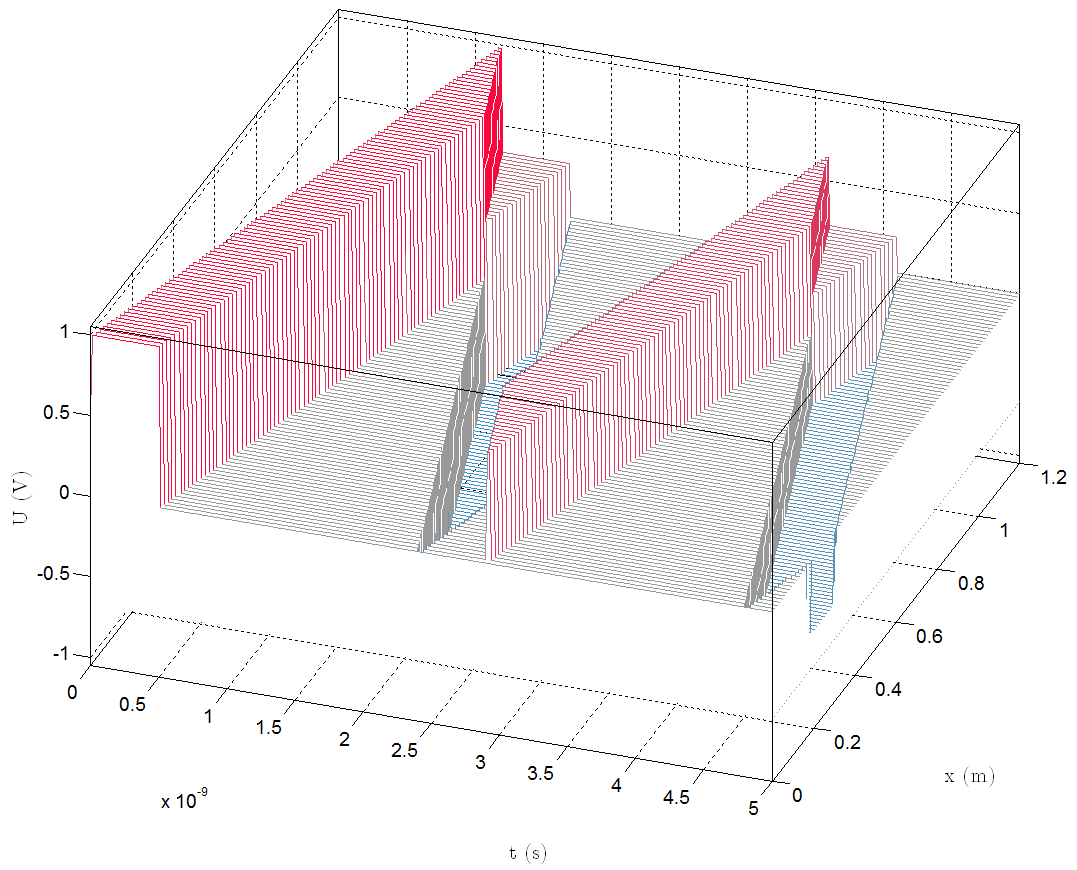
\includegraphics[width=\linewidth]{resources/Voltage100Ohm.png}
	\caption{Voltage on the transmission channel with rectangular input pulse.}
	\label{fig:voltage}
\end{figure}

\begin{figure}[H]
	\centering
	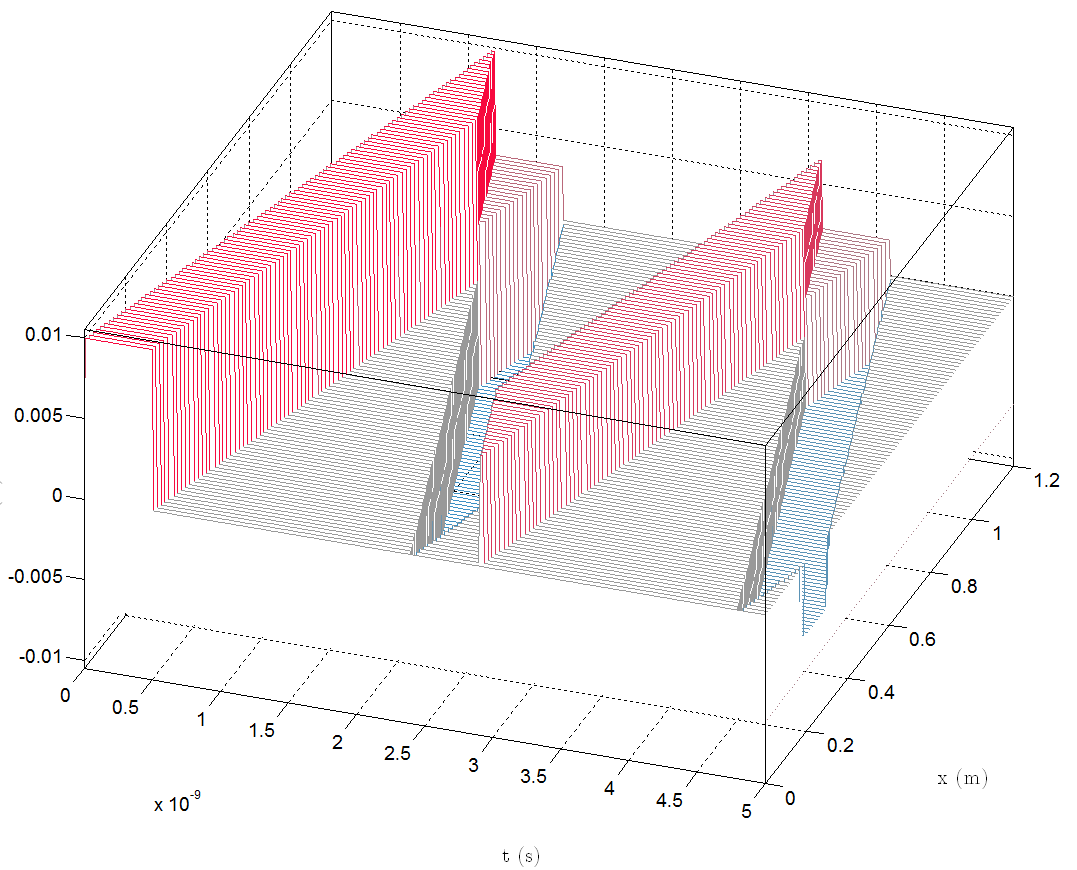
\includegraphics[width=\linewidth]{resources/Current100Ohm.png}
	\caption{Current through the transmission channel with rectangular input pulse.}
	\label{fig:current}
\end{figure}

\section{Task 4}
The load impedance $Z_l$ is changed to $50 + j50 \Omega$, while keeping the configuration of the transmission channel as in Task 3. The delivered complex power to the load will be divided into real and imaginary power, with which the power efficiency can be calculated as:

\begin{equation}
	\eta = \frac{P}{S} \cdot 100\% = \frac{P}{P + Q} \cdot 100\%
	\label{eq:efficiency}
\end{equation}

The breakdown of the power was calculated using the Matlab script \emph{task-4.m}, which is given in Appendix A. This breakdown of power delivered to the load impedance is displayed in Figure \ref{fig:breakdown}. From this figure, the power efficiency can be calculated using Eq. \ref{eq:efficiency}, which is displayed in Figure \ref{fig:efficiency}. In both figures there are two peaks, the first is the primary pulse and the second is the first reflection of this primary pulse. The reflection has less power than the primary since it had a longer route through the network and thus more losses. The imaginary part of this reflection is however smaller than the imaginary part of the primary pulse. For this reason, the efficiency of the second peak, which is the reflection, has a higher power efficiency of 98\% to the 71\% of the primary pulse.

\begin{figure}[H]
	\centering
	\setlength\figureheight{4cm}
    	\setlength\figurewidth{0.8\linewidth}
	% This file was created by matlab2tikz v0.4.6 running on MATLAB 8.2.
% Copyright (c) 2008--2014, Nico Schlömer <nico.schloemer@gmail.com>
% All rights reserved.
% Minimal pgfplots version: 1.3
% 
% The latest updates can be retrieved from
%   http://www.mathworks.com/matlabcentral/fileexchange/22022-matlab2tikz
% where you can also make suggestions and rate matlab2tikz.
% 
%
% defining custom colors
\definecolor{mycolor1}{rgb}{0.00000,0.75000,0.75000}%
\definecolor{mycolor2}{rgb}{0.75000,0.00000,0.75000}%
\definecolor{mycolor3}{rgb}{0.75000,0.75000,0.00000}%
%
\begin{tikzpicture}

\begin{axis}[%
width=\figurewidth,
height=\figureheight,
scale only axis,
xmin=0,
xmax=5e-09,
ymin=0,
ymax=0.001
]
\addplot [color=blue,solid,forget plot]
  table[row sep=crcr]{
0	0	\\
1.1e-10	0	\\
2.2e-10	0	\\
3.3e-10	0	\\
4.4e-10	0	\\
5.4e-10	0	\\
6.5e-10	0	\\
7.5e-10	0	\\
8.6e-10	0	\\
9.6e-10	0	\\
1.07e-09	0	\\
1.18e-09	0	\\
1.2e-09	0.000763235689330825	\\
1.31e-09	0.000763235689330825	\\
1.41e-09	0.000763235689330825	\\
1.51e-09	0.000763235689330825	\\
1.62e-09	0.000763235689330825	\\
1.7e-09	0	\\
1.8e-09	0	\\
1.9e-09	0	\\
2.01e-09	0	\\
2.11e-09	0	\\
2.21e-09	0	\\
2.32e-09	0	\\
2.42e-09	0	\\
2.52e-09	0	\\
2.63e-09	0	\\
2.73e-09	0	\\
2.83e-09	0	\\
2.93e-09	0	\\
3.04e-09	0	\\
3.14e-09	0	\\
3.24e-09	0	\\
3.34e-09	0	\\
3.45e-09	0	\\
3.55e-09	0	\\
3.6e-09	0.000610698909513694	\\
3.7e-09	0.000610698909513694	\\
3.8e-09	0.000610698909513694	\\
3.9e-09	0.000610698909513694	\\
4e-09	0.000610698909513694	\\
4.1e-09	0	\\
4.2e-09	0	\\
4.3e-09	0	\\
4.41e-09	0	\\
4.51e-09	0	\\
4.61e-09	0	\\
4.71e-09	0	\\
4.82e-09	0	\\
4.92e-09	0	\\
5e-09	0	\\
};
\addplot [color=black!50!green,solid,forget plot]
  table[row sep=crcr]{
0	0	\\
1.1e-10	0	\\
2.2e-10	0	\\
3.3e-10	0	\\
4.4e-10	0	\\
5.4e-10	0	\\
6.5e-10	0	\\
7.5e-10	0	\\
8.6e-10	0	\\
9.6e-10	0	\\
1.07e-09	0	\\
1.18e-09	0	\\
1.28e-09	0	\\
1.38e-09	0	\\
1.49e-09	0	\\
1.59e-09	0	\\
1.69e-09	0	\\
1.8e-09	0	\\
1.9e-09	0	\\
2.01e-09	0	\\
2.11e-09	0	\\
2.21e-09	0	\\
2.32e-09	0	\\
2.42e-09	0	\\
2.52e-09	0	\\
2.63e-09	0	\\
2.73e-09	0	\\
2.83e-09	0	\\
2.93e-09	0	\\
3.04e-09	0	\\
3.14e-09	0	\\
3.24e-09	0	\\
3.34e-09	0	\\
3.45e-09	0	\\
3.55e-09	0	\\
3.65e-09	0	\\
3.75e-09	0	\\
3.86e-09	0	\\
3.96e-09	0	\\
4.06e-09	0	\\
4.16e-09	0	\\
4.27e-09	0	\\
4.37e-09	0	\\
4.47e-09	0	\\
4.57e-09	0	\\
4.68e-09	0	\\
4.78e-09	0	\\
4.89e-09	0	\\
4.99e-09	0	\\
5e-09	0	\\
};
\addplot [color=red,solid,forget plot]
  table[row sep=crcr]{
0	0	\\
1.1e-10	0	\\
2.2e-10	0	\\
3.3e-10	0	\\
4.4e-10	0	\\
5.4e-10	0	\\
6.5e-10	0	\\
7.5e-10	0	\\
8.6e-10	0	\\
9.6e-10	0	\\
1.07e-09	0	\\
1.18e-09	0	\\
1.28e-09	0	\\
1.38e-09	0	\\
1.49e-09	0	\\
1.59e-09	0	\\
1.69e-09	0	\\
1.8e-09	0	\\
1.9e-09	0	\\
2.01e-09	0	\\
2.11e-09	0	\\
2.21e-09	0	\\
2.32e-09	0	\\
2.42e-09	0	\\
2.52e-09	0	\\
2.63e-09	0	\\
2.73e-09	0	\\
2.83e-09	0	\\
2.93e-09	0	\\
3.04e-09	0	\\
3.14e-09	0	\\
3.24e-09	0	\\
3.34e-09	0	\\
3.45e-09	0	\\
3.55e-09	0	\\
3.65e-09	0	\\
3.75e-09	0	\\
3.86e-09	0	\\
3.96e-09	0	\\
4.06e-09	0	\\
4.16e-09	0	\\
4.27e-09	0	\\
4.37e-09	0	\\
4.47e-09	0	\\
4.57e-09	0	\\
4.68e-09	0	\\
4.78e-09	0	\\
4.89e-09	0	\\
4.99e-09	0	\\
5e-09	0	\\
};
\addplot [color=mycolor1,solid,forget plot]
  table[row sep=crcr]{
0	0	\\
1.1e-10	0	\\
2.2e-10	0	\\
3.3e-10	0	\\
4.4e-10	0	\\
5.4e-10	0	\\
6.5e-10	0	\\
7.5e-10	0	\\
8.6e-10	0	\\
9.6e-10	0	\\
1.07e-09	0	\\
1.18e-09	0	\\
1.28e-09	0	\\
1.38e-09	0	\\
1.49e-09	0	\\
1.59e-09	0	\\
1.69e-09	0	\\
1.8e-09	0	\\
1.9e-09	0	\\
2.01e-09	0	\\
2.11e-09	0	\\
2.21e-09	0	\\
2.32e-09	0	\\
2.42e-09	0	\\
2.52e-09	0	\\
2.63e-09	0	\\
2.73e-09	0	\\
2.83e-09	0	\\
2.93e-09	0	\\
3.04e-09	0	\\
3.14e-09	0	\\
3.24e-09	0	\\
3.34e-09	0	\\
3.45e-09	0	\\
3.55e-09	0	\\
3.65e-09	0	\\
3.75e-09	0	\\
3.86e-09	0	\\
3.96e-09	0	\\
4.06e-09	0	\\
4.16e-09	0	\\
4.27e-09	0	\\
4.37e-09	0	\\
4.47e-09	0	\\
4.57e-09	0	\\
4.68e-09	0	\\
4.78e-09	0	\\
4.89e-09	0	\\
4.99e-09	0	\\
5e-09	0	\\
};
\addplot [color=mycolor2,solid,forget plot]
  table[row sep=crcr]{
0	0	\\
1.1e-10	0	\\
2.2e-10	0	\\
3.3e-10	0	\\
4.4e-10	0	\\
5.4e-10	0	\\
6.5e-10	0	\\
7.5e-10	0	\\
8.6e-10	0	\\
9.6e-10	0	\\
1.07e-09	0	\\
1.18e-09	0	\\
1.28e-09	0	\\
1.38e-09	0	\\
1.49e-09	0	\\
1.59e-09	0	\\
1.69e-09	0	\\
1.8e-09	0	\\
1.9e-09	0	\\
2.01e-09	0	\\
2.11e-09	0	\\
2.21e-09	0	\\
2.32e-09	0	\\
2.42e-09	0	\\
2.52e-09	0	\\
2.63e-09	0	\\
2.73e-09	0	\\
2.83e-09	0	\\
2.93e-09	0	\\
3.04e-09	0	\\
3.14e-09	0	\\
3.24e-09	0	\\
3.34e-09	0	\\
3.45e-09	0	\\
3.55e-09	0	\\
3.65e-09	0	\\
3.75e-09	0	\\
3.86e-09	0	\\
3.96e-09	0	\\
4.06e-09	0	\\
4.16e-09	0	\\
4.27e-09	0	\\
4.37e-09	0	\\
4.47e-09	0	\\
4.57e-09	0	\\
4.68e-09	0	\\
4.78e-09	0	\\
4.89e-09	0	\\
4.99e-09	0	\\
5e-09	0	\\
};
\addplot [color=mycolor3,solid,forget plot]
  table[row sep=crcr]{
0	0	\\
1.1e-10	0	\\
2.2e-10	0	\\
3.3e-10	0	\\
4.4e-10	0	\\
5.4e-10	0	\\
6.5e-10	0	\\
7.5e-10	0	\\
8.6e-10	0	\\
9.6e-10	0	\\
1.07e-09	0	\\
1.18e-09	0	\\
1.28e-09	0	\\
1.38e-09	0	\\
1.49e-09	0	\\
1.59e-09	0	\\
1.69e-09	0	\\
1.8e-09	0	\\
1.9e-09	0	\\
2.01e-09	0	\\
2.11e-09	0	\\
2.21e-09	0	\\
2.32e-09	0	\\
2.42e-09	0	\\
2.52e-09	0	\\
2.63e-09	0	\\
2.73e-09	0	\\
2.83e-09	0	\\
2.93e-09	0	\\
3.04e-09	0	\\
3.14e-09	0	\\
3.24e-09	0	\\
3.34e-09	0	\\
3.45e-09	0	\\
3.55e-09	0	\\
3.65e-09	0	\\
3.75e-09	0	\\
3.86e-09	0	\\
3.96e-09	0	\\
4.06e-09	0	\\
4.16e-09	0	\\
4.27e-09	0	\\
4.37e-09	0	\\
4.47e-09	0	\\
4.57e-09	0	\\
4.68e-09	0	\\
4.78e-09	0	\\
4.89e-09	0	\\
4.99e-09	0	\\
5e-09	0	\\
};
\addplot [color=darkgray,solid,forget plot]
  table[row sep=crcr]{
0	0	\\
1.1e-10	0	\\
2.2e-10	0	\\
3.3e-10	0	\\
4.4e-10	0	\\
5.4e-10	0	\\
6.5e-10	0	\\
7.5e-10	0	\\
8.6e-10	0	\\
9.6e-10	0	\\
1.07e-09	0	\\
1.18e-09	0	\\
1.28e-09	0	\\
1.38e-09	0	\\
1.49e-09	0	\\
1.59e-09	0	\\
1.69e-09	0	\\
1.8e-09	0	\\
1.9e-09	0	\\
2.01e-09	0	\\
2.11e-09	0	\\
2.21e-09	0	\\
2.32e-09	0	\\
2.42e-09	0	\\
2.52e-09	0	\\
2.63e-09	0	\\
2.73e-09	0	\\
2.83e-09	0	\\
2.93e-09	0	\\
3.04e-09	0	\\
3.14e-09	0	\\
3.24e-09	0	\\
3.34e-09	0	\\
3.45e-09	0	\\
3.55e-09	0	\\
3.65e-09	0	\\
3.75e-09	0	\\
3.86e-09	0	\\
3.96e-09	0	\\
4.06e-09	0	\\
4.16e-09	0	\\
4.27e-09	0	\\
4.37e-09	0	\\
4.47e-09	0	\\
4.57e-09	0	\\
4.68e-09	0	\\
4.78e-09	0	\\
4.89e-09	0	\\
4.99e-09	0	\\
5e-09	0	\\
};
\addplot [color=blue,solid,forget plot]
  table[row sep=crcr]{
0	0	\\
1.1e-10	0	\\
2.2e-10	0	\\
3.3e-10	0	\\
4.4e-10	0	\\
5.4e-10	0	\\
6.5e-10	0	\\
7.5e-10	0	\\
8.6e-10	0	\\
9.6e-10	0	\\
1.07e-09	0	\\
1.18e-09	0	\\
1.28e-09	0	\\
1.38e-09	0	\\
1.49e-09	0	\\
1.59e-09	0	\\
1.69e-09	0	\\
1.8e-09	0	\\
1.9e-09	0	\\
2.01e-09	0	\\
2.11e-09	0	\\
2.21e-09	0	\\
2.32e-09	0	\\
2.42e-09	0	\\
2.52e-09	0	\\
2.63e-09	0	\\
2.73e-09	0	\\
2.83e-09	0	\\
2.93e-09	0	\\
3.04e-09	0	\\
3.14e-09	0	\\
3.24e-09	0	\\
3.34e-09	0	\\
3.45e-09	0	\\
3.55e-09	0	\\
3.65e-09	0	\\
3.75e-09	0	\\
3.86e-09	0	\\
3.96e-09	0	\\
4.06e-09	0	\\
4.16e-09	0	\\
4.27e-09	0	\\
4.37e-09	0	\\
4.47e-09	0	\\
4.57e-09	0	\\
4.68e-09	0	\\
4.78e-09	0	\\
4.89e-09	0	\\
4.99e-09	0	\\
5e-09	0	\\
};
\addplot [color=black!50!green,solid,forget plot]
  table[row sep=crcr]{
0	0	\\
1.1e-10	0	\\
2.2e-10	0	\\
3.3e-10	0	\\
4.4e-10	0	\\
5.4e-10	0	\\
6.5e-10	0	\\
7.5e-10	0	\\
8.6e-10	0	\\
9.6e-10	0	\\
1.07e-09	0	\\
1.18e-09	0	\\
1.28e-09	0	\\
1.38e-09	0	\\
1.49e-09	0	\\
1.59e-09	0	\\
1.69e-09	0	\\
1.8e-09	0	\\
1.9e-09	0	\\
2.01e-09	0	\\
2.11e-09	0	\\
2.21e-09	0	\\
2.32e-09	0	\\
2.42e-09	0	\\
2.52e-09	0	\\
2.63e-09	0	\\
2.73e-09	0	\\
2.83e-09	0	\\
2.93e-09	0	\\
3.04e-09	0	\\
3.14e-09	0	\\
3.24e-09	0	\\
3.34e-09	0	\\
3.45e-09	0	\\
3.55e-09	0	\\
3.65e-09	0	\\
3.75e-09	0	\\
3.86e-09	0	\\
3.96e-09	0	\\
4.06e-09	0	\\
4.16e-09	0	\\
4.27e-09	0	\\
4.37e-09	0	\\
4.47e-09	0	\\
4.57e-09	0	\\
4.68e-09	0	\\
4.78e-09	0	\\
4.89e-09	0	\\
4.99e-09	0	\\
5e-09	0	\\
};
\addplot [color=red,solid,forget plot]
  table[row sep=crcr]{
0	0	\\
1.1e-10	0	\\
2.2e-10	0	\\
3.3e-10	0	\\
4.4e-10	0	\\
5.4e-10	0	\\
6.5e-10	0	\\
7.5e-10	0	\\
8.6e-10	0	\\
9.6e-10	0	\\
1.07e-09	0	\\
1.18e-09	0	\\
1.28e-09	0	\\
1.38e-09	0	\\
1.49e-09	0	\\
1.59e-09	0	\\
1.69e-09	0	\\
1.8e-09	0	\\
1.9e-09	0	\\
2.01e-09	0	\\
2.11e-09	0	\\
2.21e-09	0	\\
2.32e-09	0	\\
2.42e-09	0	\\
2.52e-09	0	\\
2.63e-09	0	\\
2.73e-09	0	\\
2.83e-09	0	\\
2.93e-09	0	\\
3.04e-09	0	\\
3.14e-09	0	\\
3.24e-09	0	\\
3.34e-09	0	\\
3.45e-09	0	\\
3.55e-09	0	\\
3.65e-09	0	\\
3.75e-09	0	\\
3.86e-09	0	\\
3.96e-09	0	\\
4.06e-09	0	\\
4.16e-09	0	\\
4.27e-09	0	\\
4.37e-09	0	\\
4.47e-09	0	\\
4.57e-09	0	\\
4.68e-09	0	\\
4.78e-09	0	\\
4.89e-09	0	\\
4.99e-09	0	\\
5e-09	0	\\
};
\addplot [color=mycolor1,solid,forget plot]
  table[row sep=crcr]{
0	0	\\
1.1e-10	0	\\
2.2e-10	0	\\
3.3e-10	0	\\
4.4e-10	0	\\
5.4e-10	0	\\
6.5e-10	0	\\
7.5e-10	0	\\
8.6e-10	0	\\
9.6e-10	0	\\
1.07e-09	0	\\
1.18e-09	0	\\
1.28e-09	0	\\
1.38e-09	0	\\
1.49e-09	0	\\
1.59e-09	0	\\
1.69e-09	0	\\
1.8e-09	0	\\
1.9e-09	0	\\
2.01e-09	0	\\
2.11e-09	0	\\
2.21e-09	0	\\
2.32e-09	0	\\
2.42e-09	0	\\
2.52e-09	0	\\
2.63e-09	0	\\
2.73e-09	0	\\
2.83e-09	0	\\
2.93e-09	0	\\
3.04e-09	0	\\
3.14e-09	0	\\
3.24e-09	0	\\
3.34e-09	0	\\
3.45e-09	0	\\
3.55e-09	0	\\
3.65e-09	0	\\
3.75e-09	0	\\
3.86e-09	0	\\
3.96e-09	0	\\
4.06e-09	0	\\
4.16e-09	0	\\
4.27e-09	0	\\
4.37e-09	0	\\
4.47e-09	0	\\
4.57e-09	0	\\
4.68e-09	0	\\
4.78e-09	0	\\
4.89e-09	0	\\
4.99e-09	0	\\
5e-09	0	\\
};
\addplot [color=mycolor2,solid,forget plot]
  table[row sep=crcr]{
0	0	\\
1.1e-10	0	\\
2.2e-10	0	\\
3.3e-10	0	\\
4.4e-10	0	\\
5.4e-10	0	\\
6.5e-10	0	\\
7.5e-10	0	\\
8.6e-10	0	\\
9.6e-10	0	\\
1.07e-09	0	\\
1.18e-09	0	\\
1.28e-09	0	\\
1.38e-09	0	\\
1.49e-09	0	\\
1.59e-09	0	\\
1.69e-09	0	\\
1.8e-09	0	\\
1.9e-09	0	\\
2.01e-09	0	\\
2.11e-09	0	\\
2.21e-09	0	\\
2.32e-09	0	\\
2.42e-09	0	\\
2.52e-09	0	\\
2.63e-09	0	\\
2.73e-09	0	\\
2.83e-09	0	\\
2.93e-09	0	\\
3.04e-09	0	\\
3.14e-09	0	\\
3.24e-09	0	\\
3.34e-09	0	\\
3.45e-09	0	\\
3.55e-09	0	\\
3.65e-09	0	\\
3.75e-09	0	\\
3.86e-09	0	\\
3.96e-09	0	\\
4.06e-09	0	\\
4.16e-09	0	\\
4.27e-09	0	\\
4.37e-09	0	\\
4.47e-09	0	\\
4.57e-09	0	\\
4.68e-09	0	\\
4.78e-09	0	\\
4.89e-09	0	\\
4.99e-09	0	\\
5e-09	0	\\
};
\addplot [color=mycolor3,solid,forget plot]
  table[row sep=crcr]{
0	0	\\
1.1e-10	0	\\
2.2e-10	0	\\
3.3e-10	0	\\
4.4e-10	0	\\
5.4e-10	0	\\
6.5e-10	0	\\
7.5e-10	0	\\
8.6e-10	0	\\
9.6e-10	0	\\
1.07e-09	0	\\
1.18e-09	0	\\
1.28e-09	0	\\
1.38e-09	0	\\
1.49e-09	0	\\
1.59e-09	0	\\
1.69e-09	0	\\
1.8e-09	0	\\
1.9e-09	0	\\
2.01e-09	0	\\
2.11e-09	0	\\
2.21e-09	0	\\
2.32e-09	0	\\
2.42e-09	0	\\
2.52e-09	0	\\
2.63e-09	0	\\
2.73e-09	0	\\
2.83e-09	0	\\
2.93e-09	0	\\
3.04e-09	0	\\
3.14e-09	0	\\
3.24e-09	0	\\
3.34e-09	0	\\
3.45e-09	0	\\
3.55e-09	0	\\
3.65e-09	0	\\
3.75e-09	0	\\
3.86e-09	0	\\
3.96e-09	0	\\
4.06e-09	0	\\
4.16e-09	0	\\
4.27e-09	0	\\
4.37e-09	0	\\
4.47e-09	0	\\
4.57e-09	0	\\
4.68e-09	0	\\
4.78e-09	0	\\
4.89e-09	0	\\
4.99e-09	0	\\
5e-09	0	\\
};
\addplot [color=darkgray,solid,forget plot]
  table[row sep=crcr]{
0	0	\\
1.1e-10	0	\\
2.2e-10	0	\\
3.3e-10	0	\\
4.4e-10	0	\\
5.4e-10	0	\\
6.5e-10	0	\\
7.5e-10	0	\\
8.6e-10	0	\\
9.6e-10	0	\\
1.07e-09	0	\\
1.18e-09	0	\\
1.28e-09	0	\\
1.38e-09	0	\\
1.49e-09	0	\\
1.59e-09	0	\\
1.69e-09	0	\\
1.8e-09	0	\\
1.9e-09	0	\\
2.01e-09	0	\\
2.11e-09	0	\\
2.21e-09	0	\\
2.32e-09	0	\\
2.42e-09	0	\\
2.52e-09	0	\\
2.63e-09	0	\\
2.73e-09	0	\\
2.83e-09	0	\\
2.93e-09	0	\\
3.04e-09	0	\\
3.14e-09	0	\\
3.24e-09	0	\\
3.34e-09	0	\\
3.45e-09	0	\\
3.55e-09	0	\\
3.65e-09	0	\\
3.75e-09	0	\\
3.86e-09	0	\\
3.96e-09	0	\\
4.06e-09	0	\\
4.16e-09	0	\\
4.27e-09	0	\\
4.37e-09	0	\\
4.47e-09	0	\\
4.57e-09	0	\\
4.68e-09	0	\\
4.78e-09	0	\\
4.89e-09	0	\\
4.99e-09	0	\\
5e-09	0	\\
};
\addplot [color=blue,solid,forget plot]
  table[row sep=crcr]{
0	0	\\
1.1e-10	0	\\
2.2e-10	0	\\
3.3e-10	0	\\
4.4e-10	0	\\
5.4e-10	0	\\
6.5e-10	0	\\
7.5e-10	0	\\
8.6e-10	0	\\
9.6e-10	0	\\
1.07e-09	0	\\
1.18e-09	0	\\
1.28e-09	0	\\
1.38e-09	0	\\
1.49e-09	0	\\
1.59e-09	0	\\
1.69e-09	0	\\
1.8e-09	0	\\
1.9e-09	0	\\
2.01e-09	0	\\
2.11e-09	0	\\
2.21e-09	0	\\
2.32e-09	0	\\
2.42e-09	0	\\
2.52e-09	0	\\
2.63e-09	0	\\
2.73e-09	0	\\
2.83e-09	0	\\
2.93e-09	0	\\
3.04e-09	0	\\
3.14e-09	0	\\
3.24e-09	0	\\
3.34e-09	0	\\
3.45e-09	0	\\
3.55e-09	0	\\
3.65e-09	0	\\
3.75e-09	0	\\
3.86e-09	0	\\
3.96e-09	0	\\
4.06e-09	0	\\
4.16e-09	0	\\
4.27e-09	0	\\
4.37e-09	0	\\
4.47e-09	0	\\
4.57e-09	0	\\
4.68e-09	0	\\
4.78e-09	0	\\
4.89e-09	0	\\
4.99e-09	0	\\
5e-09	0	\\
};
\addplot [color=black!50!green,solid,forget plot]
  table[row sep=crcr]{
0	0	\\
1.1e-10	0	\\
2.2e-10	0	\\
3.3e-10	0	\\
4.4e-10	0	\\
5.4e-10	0	\\
6.5e-10	0	\\
7.5e-10	0	\\
8.6e-10	0	\\
9.6e-10	0	\\
1.07e-09	0	\\
1.18e-09	0	\\
1.28e-09	0	\\
1.38e-09	0	\\
1.49e-09	0	\\
1.59e-09	0	\\
1.69e-09	0	\\
1.8e-09	0	\\
1.9e-09	0	\\
2.01e-09	0	\\
2.11e-09	0	\\
2.21e-09	0	\\
2.32e-09	0	\\
2.42e-09	0	\\
2.52e-09	0	\\
2.63e-09	0	\\
2.73e-09	0	\\
2.83e-09	0	\\
2.93e-09	0	\\
3.04e-09	0	\\
3.14e-09	0	\\
3.24e-09	0	\\
3.34e-09	0	\\
3.45e-09	0	\\
3.55e-09	0	\\
3.65e-09	0	\\
3.75e-09	0	\\
3.86e-09	0	\\
3.96e-09	0	\\
4.06e-09	0	\\
4.16e-09	0	\\
4.27e-09	0	\\
4.37e-09	0	\\
4.47e-09	0	\\
4.57e-09	0	\\
4.68e-09	0	\\
4.78e-09	0	\\
4.89e-09	0	\\
4.99e-09	0	\\
5e-09	0	\\
};
\addplot [color=red,solid,forget plot]
  table[row sep=crcr]{
0	0	\\
1.1e-10	0	\\
2.2e-10	0	\\
3.3e-10	0	\\
4.4e-10	0	\\
5.4e-10	0	\\
6.5e-10	0	\\
7.5e-10	0	\\
8.6e-10	0	\\
9.6e-10	0	\\
1.07e-09	0	\\
1.18e-09	0	\\
1.28e-09	0	\\
1.38e-09	0	\\
1.49e-09	0	\\
1.59e-09	0	\\
1.69e-09	0	\\
1.8e-09	0	\\
1.9e-09	0	\\
2.01e-09	0	\\
2.11e-09	0	\\
2.21e-09	0	\\
2.32e-09	0	\\
2.42e-09	0	\\
2.52e-09	0	\\
2.63e-09	0	\\
2.73e-09	0	\\
2.83e-09	0	\\
2.93e-09	0	\\
3.04e-09	0	\\
3.14e-09	0	\\
3.24e-09	0	\\
3.34e-09	0	\\
3.45e-09	0	\\
3.55e-09	0	\\
3.65e-09	0	\\
3.75e-09	0	\\
3.86e-09	0	\\
3.96e-09	0	\\
4.06e-09	0	\\
4.16e-09	0	\\
4.27e-09	0	\\
4.37e-09	0	\\
4.47e-09	0	\\
4.57e-09	0	\\
4.68e-09	0	\\
4.78e-09	0	\\
4.89e-09	0	\\
4.99e-09	0	\\
5e-09	0	\\
};
\addplot [color=mycolor1,solid,forget plot]
  table[row sep=crcr]{
0	0	\\
1.1e-10	0	\\
2.2e-10	0	\\
3.3e-10	0	\\
4.4e-10	0	\\
5.4e-10	0	\\
6.5e-10	0	\\
7.5e-10	0	\\
8.6e-10	0	\\
9.6e-10	0	\\
1.07e-09	0	\\
1.18e-09	0	\\
1.28e-09	0	\\
1.38e-09	0	\\
1.49e-09	0	\\
1.59e-09	0	\\
1.69e-09	0	\\
1.8e-09	0	\\
1.9e-09	0	\\
2.01e-09	0	\\
2.11e-09	0	\\
2.21e-09	0	\\
2.32e-09	0	\\
2.42e-09	0	\\
2.52e-09	0	\\
2.63e-09	0	\\
2.73e-09	0	\\
2.83e-09	0	\\
2.93e-09	0	\\
3.04e-09	0	\\
3.14e-09	0	\\
3.24e-09	0	\\
3.34e-09	0	\\
3.45e-09	0	\\
3.55e-09	0	\\
3.65e-09	0	\\
3.75e-09	0	\\
3.86e-09	0	\\
3.96e-09	0	\\
4.06e-09	0	\\
4.16e-09	0	\\
4.27e-09	0	\\
4.37e-09	0	\\
4.47e-09	0	\\
4.57e-09	0	\\
4.68e-09	0	\\
4.78e-09	0	\\
4.89e-09	0	\\
4.99e-09	0	\\
5e-09	0	\\
};
\addplot [color=mycolor2,solid,forget plot]
  table[row sep=crcr]{
0	0	\\
1.1e-10	0	\\
2.2e-10	0	\\
3.3e-10	0	\\
4.4e-10	0	\\
5.4e-10	0	\\
6.5e-10	0	\\
7.5e-10	0	\\
8.6e-10	0	\\
9.6e-10	0	\\
1.07e-09	0	\\
1.18e-09	0	\\
1.28e-09	0	\\
1.38e-09	0	\\
1.49e-09	0	\\
1.59e-09	0	\\
1.69e-09	0	\\
1.8e-09	0	\\
1.9e-09	0	\\
2.01e-09	0	\\
2.11e-09	0	\\
2.21e-09	0	\\
2.32e-09	0	\\
2.42e-09	0	\\
2.52e-09	0	\\
2.63e-09	0	\\
2.73e-09	0	\\
2.83e-09	0	\\
2.93e-09	0	\\
3.04e-09	0	\\
3.14e-09	0	\\
3.24e-09	0	\\
3.34e-09	0	\\
3.45e-09	0	\\
3.55e-09	0	\\
3.65e-09	0	\\
3.75e-09	0	\\
3.86e-09	0	\\
3.96e-09	0	\\
4.06e-09	0	\\
4.16e-09	0	\\
4.27e-09	0	\\
4.37e-09	0	\\
4.47e-09	0	\\
4.57e-09	0	\\
4.68e-09	0	\\
4.78e-09	0	\\
4.89e-09	0	\\
4.99e-09	0	\\
5e-09	0	\\
};
\addplot [color=mycolor3,solid,forget plot]
  table[row sep=crcr]{
0	0	\\
1.1e-10	0	\\
2.2e-10	0	\\
3.3e-10	0	\\
4.4e-10	0	\\
5.4e-10	0	\\
6.5e-10	0	\\
7.5e-10	0	\\
8.6e-10	0	\\
9.6e-10	0	\\
1.07e-09	0	\\
1.18e-09	0	\\
1.28e-09	0	\\
1.38e-09	0	\\
1.49e-09	0	\\
1.59e-09	0	\\
1.69e-09	0	\\
1.8e-09	0	\\
1.9e-09	0	\\
2.01e-09	0	\\
2.11e-09	0	\\
2.21e-09	0	\\
2.32e-09	0	\\
2.42e-09	0	\\
2.52e-09	0	\\
2.63e-09	0	\\
2.73e-09	0	\\
2.83e-09	0	\\
2.93e-09	0	\\
3.04e-09	0	\\
3.14e-09	0	\\
3.24e-09	0	\\
3.34e-09	0	\\
3.45e-09	0	\\
3.55e-09	0	\\
3.65e-09	0	\\
3.75e-09	0	\\
3.86e-09	0	\\
3.96e-09	0	\\
4.06e-09	0	\\
4.16e-09	0	\\
4.27e-09	0	\\
4.37e-09	0	\\
4.47e-09	0	\\
4.57e-09	0	\\
4.68e-09	0	\\
4.78e-09	0	\\
4.89e-09	0	\\
4.99e-09	0	\\
5e-09	0	\\
};
\addplot [color=darkgray,solid,forget plot]
  table[row sep=crcr]{
0	0	\\
1.1e-10	0	\\
2.2e-10	0	\\
3.3e-10	0	\\
4.4e-10	0	\\
5.4e-10	0	\\
6.5e-10	0	\\
7.5e-10	0	\\
8.6e-10	0	\\
9.6e-10	0	\\
1.07e-09	0	\\
1.18e-09	0	\\
1.28e-09	0	\\
1.38e-09	0	\\
1.49e-09	0	\\
1.59e-09	0	\\
1.69e-09	0	\\
1.8e-09	0	\\
1.9e-09	0	\\
2.01e-09	0	\\
2.11e-09	0	\\
2.21e-09	0	\\
2.32e-09	0	\\
2.42e-09	0	\\
2.52e-09	0	\\
2.63e-09	0	\\
2.73e-09	0	\\
2.83e-09	0	\\
2.93e-09	0	\\
3.04e-09	0	\\
3.14e-09	0	\\
3.24e-09	0	\\
3.34e-09	0	\\
3.45e-09	0	\\
3.55e-09	0	\\
3.65e-09	0	\\
3.75e-09	0	\\
3.86e-09	0	\\
3.96e-09	0	\\
4.06e-09	0	\\
4.16e-09	0	\\
4.27e-09	0	\\
4.37e-09	0	\\
4.47e-09	0	\\
4.57e-09	0	\\
4.68e-09	0	\\
4.78e-09	0	\\
4.89e-09	0	\\
4.99e-09	0	\\
5e-09	0	\\
};
\addplot [color=blue,solid,forget plot]
  table[row sep=crcr]{
0	0	\\
1.1e-10	0	\\
2.2e-10	0	\\
3.3e-10	0	\\
4.4e-10	0	\\
5.4e-10	0	\\
6.5e-10	0	\\
7.5e-10	0	\\
8.6e-10	0	\\
9.6e-10	0	\\
1.07e-09	0	\\
1.18e-09	0	\\
1.28e-09	0	\\
1.38e-09	0	\\
1.49e-09	0	\\
1.59e-09	0	\\
1.69e-09	0	\\
1.8e-09	0	\\
1.9e-09	0	\\
2.01e-09	0	\\
2.11e-09	0	\\
2.21e-09	0	\\
2.32e-09	0	\\
2.42e-09	0	\\
2.52e-09	0	\\
2.63e-09	0	\\
2.73e-09	0	\\
2.83e-09	0	\\
2.93e-09	0	\\
3.04e-09	0	\\
3.14e-09	0	\\
3.24e-09	0	\\
3.34e-09	0	\\
3.45e-09	0	\\
3.55e-09	0	\\
3.65e-09	0	\\
3.75e-09	0	\\
3.86e-09	0	\\
3.96e-09	0	\\
4.06e-09	0	\\
4.16e-09	0	\\
4.27e-09	0	\\
4.37e-09	0	\\
4.47e-09	0	\\
4.57e-09	0	\\
4.68e-09	0	\\
4.78e-09	0	\\
4.89e-09	0	\\
4.99e-09	0	\\
5e-09	0	\\
};
\addplot [color=black!50!green,solid,forget plot]
  table[row sep=crcr]{
0	0	\\
1.1e-10	0	\\
2.2e-10	0	\\
3.3e-10	0	\\
4.4e-10	0	\\
5.4e-10	0	\\
6.5e-10	0	\\
7.5e-10	0	\\
8.6e-10	0	\\
9.6e-10	0	\\
1.07e-09	0	\\
1.18e-09	0	\\
1.28e-09	0	\\
1.38e-09	0	\\
1.49e-09	0	\\
1.59e-09	0	\\
1.69e-09	0	\\
1.8e-09	0	\\
1.9e-09	0	\\
2.01e-09	0	\\
2.11e-09	0	\\
2.21e-09	0	\\
2.32e-09	0	\\
2.42e-09	0	\\
2.52e-09	0	\\
2.63e-09	0	\\
2.73e-09	0	\\
2.83e-09	0	\\
2.93e-09	0	\\
3.04e-09	0	\\
3.14e-09	0	\\
3.24e-09	0	\\
3.34e-09	0	\\
3.45e-09	0	\\
3.55e-09	0	\\
3.65e-09	0	\\
3.75e-09	0	\\
3.86e-09	0	\\
3.96e-09	0	\\
4.06e-09	0	\\
4.16e-09	0	\\
4.27e-09	0	\\
4.37e-09	0	\\
4.47e-09	0	\\
4.57e-09	0	\\
4.68e-09	0	\\
4.78e-09	0	\\
4.89e-09	0	\\
4.99e-09	0	\\
5e-09	0	\\
};
\addplot [color=red,solid,forget plot]
  table[row sep=crcr]{
0	0	\\
1.1e-10	0	\\
2.2e-10	0	\\
3.3e-10	0	\\
4.4e-10	0	\\
5.4e-10	0	\\
6.5e-10	0	\\
7.5e-10	0	\\
8.6e-10	0	\\
9.6e-10	0	\\
1.07e-09	0	\\
1.18e-09	0	\\
1.28e-09	0	\\
1.38e-09	0	\\
1.49e-09	0	\\
1.59e-09	0	\\
1.69e-09	0	\\
1.8e-09	0	\\
1.9e-09	0	\\
2.01e-09	0	\\
2.11e-09	0	\\
2.21e-09	0	\\
2.32e-09	0	\\
2.42e-09	0	\\
2.52e-09	0	\\
2.63e-09	0	\\
2.73e-09	0	\\
2.83e-09	0	\\
2.93e-09	0	\\
3.04e-09	0	\\
3.14e-09	0	\\
3.24e-09	0	\\
3.34e-09	0	\\
3.45e-09	0	\\
3.55e-09	0	\\
3.65e-09	0	\\
3.75e-09	0	\\
3.86e-09	0	\\
3.96e-09	0	\\
4.06e-09	0	\\
4.16e-09	0	\\
4.27e-09	0	\\
4.37e-09	0	\\
4.47e-09	0	\\
4.57e-09	0	\\
4.68e-09	0	\\
4.78e-09	0	\\
4.89e-09	0	\\
4.99e-09	0	\\
5e-09	0	\\
};
\addplot [color=mycolor1,solid,forget plot]
  table[row sep=crcr]{
0	0	\\
1.1e-10	0	\\
2.2e-10	0	\\
3.3e-10	0	\\
4.4e-10	0	\\
5.4e-10	0	\\
6.5e-10	0	\\
7.5e-10	0	\\
8.6e-10	0	\\
9.6e-10	0	\\
1.07e-09	0	\\
1.18e-09	0	\\
1.28e-09	0	\\
1.38e-09	0	\\
1.49e-09	0	\\
1.59e-09	0	\\
1.69e-09	0	\\
1.8e-09	0	\\
1.9e-09	0	\\
2.01e-09	0	\\
2.11e-09	0	\\
2.21e-09	0	\\
2.32e-09	0	\\
2.42e-09	0	\\
2.52e-09	0	\\
2.63e-09	0	\\
2.73e-09	0	\\
2.83e-09	0	\\
2.93e-09	0	\\
3.04e-09	0	\\
3.14e-09	0	\\
3.24e-09	0	\\
3.34e-09	0	\\
3.45e-09	0	\\
3.55e-09	0	\\
3.65e-09	0	\\
3.75e-09	0	\\
3.86e-09	0	\\
3.96e-09	0	\\
4.06e-09	0	\\
4.16e-09	0	\\
4.27e-09	0	\\
4.37e-09	0	\\
4.47e-09	0	\\
4.57e-09	0	\\
4.68e-09	0	\\
4.78e-09	0	\\
4.89e-09	0	\\
4.99e-09	0	\\
5e-09	0	\\
};
\addplot [color=mycolor2,solid,forget plot]
  table[row sep=crcr]{
0	0	\\
1.1e-10	0	\\
2.2e-10	0	\\
3.3e-10	0	\\
4.4e-10	0	\\
5.4e-10	0	\\
6.5e-10	0	\\
7.5e-10	0	\\
8.6e-10	0	\\
9.6e-10	0	\\
1.07e-09	0	\\
1.18e-09	0	\\
1.28e-09	0	\\
1.38e-09	0	\\
1.49e-09	0	\\
1.59e-09	0	\\
1.69e-09	0	\\
1.8e-09	0	\\
1.9e-09	0	\\
2.01e-09	0	\\
2.11e-09	0	\\
2.21e-09	0	\\
2.32e-09	0	\\
2.42e-09	0	\\
2.52e-09	0	\\
2.63e-09	0	\\
2.73e-09	0	\\
2.83e-09	0	\\
2.93e-09	0	\\
3.04e-09	0	\\
3.14e-09	0	\\
3.24e-09	0	\\
3.34e-09	0	\\
3.45e-09	0	\\
3.55e-09	0	\\
3.65e-09	0	\\
3.75e-09	0	\\
3.86e-09	0	\\
3.96e-09	0	\\
4.06e-09	0	\\
4.16e-09	0	\\
4.27e-09	0	\\
4.37e-09	0	\\
4.47e-09	0	\\
4.57e-09	0	\\
4.68e-09	0	\\
4.78e-09	0	\\
4.89e-09	0	\\
4.99e-09	0	\\
5e-09	0	\\
};
\addplot [color=mycolor3,solid,forget plot]
  table[row sep=crcr]{
0	0	\\
1.1e-10	0	\\
2.2e-10	0	\\
3.3e-10	0	\\
4.4e-10	0	\\
5.4e-10	0	\\
6.5e-10	0	\\
7.5e-10	0	\\
8.6e-10	0	\\
9.6e-10	0	\\
1.07e-09	0	\\
1.18e-09	0	\\
1.28e-09	0	\\
1.38e-09	0	\\
1.49e-09	0	\\
1.59e-09	0	\\
1.69e-09	0	\\
1.8e-09	0	\\
1.9e-09	0	\\
2.01e-09	0	\\
2.11e-09	0	\\
2.21e-09	0	\\
2.32e-09	0	\\
2.42e-09	0	\\
2.52e-09	0	\\
2.63e-09	0	\\
2.73e-09	0	\\
2.83e-09	0	\\
2.93e-09	0	\\
3.04e-09	0	\\
3.14e-09	0	\\
3.24e-09	0	\\
3.34e-09	0	\\
3.45e-09	0	\\
3.55e-09	0	\\
3.65e-09	0	\\
3.75e-09	0	\\
3.86e-09	0	\\
3.96e-09	0	\\
4.06e-09	0	\\
4.16e-09	0	\\
4.27e-09	0	\\
4.37e-09	0	\\
4.47e-09	0	\\
4.57e-09	0	\\
4.68e-09	0	\\
4.78e-09	0	\\
4.89e-09	0	\\
4.99e-09	0	\\
5e-09	0	\\
};
\addplot [color=darkgray,solid,forget plot]
  table[row sep=crcr]{
0	0	\\
1.1e-10	0	\\
2.2e-10	0	\\
3.3e-10	0	\\
4.4e-10	0	\\
5.4e-10	0	\\
6.5e-10	0	\\
7.5e-10	0	\\
8.6e-10	0	\\
9.6e-10	0	\\
1.07e-09	0	\\
1.18e-09	0	\\
1.28e-09	0	\\
1.38e-09	0	\\
1.49e-09	0	\\
1.59e-09	0	\\
1.69e-09	0	\\
1.8e-09	0	\\
1.9e-09	0	\\
2.01e-09	0	\\
2.11e-09	0	\\
2.21e-09	0	\\
2.32e-09	0	\\
2.42e-09	0	\\
2.52e-09	0	\\
2.63e-09	0	\\
2.73e-09	0	\\
2.83e-09	0	\\
2.93e-09	0	\\
3.04e-09	0	\\
3.14e-09	0	\\
3.24e-09	0	\\
3.34e-09	0	\\
3.45e-09	0	\\
3.55e-09	0	\\
3.65e-09	0	\\
3.75e-09	0	\\
3.86e-09	0	\\
3.96e-09	0	\\
4.06e-09	0	\\
4.16e-09	0	\\
4.27e-09	0	\\
4.37e-09	0	\\
4.47e-09	0	\\
4.57e-09	0	\\
4.68e-09	0	\\
4.78e-09	0	\\
4.89e-09	0	\\
4.99e-09	0	\\
5e-09	0	\\
};
\addplot [color=blue,solid,forget plot]
  table[row sep=crcr]{
0	0	\\
1.1e-10	0	\\
2.2e-10	0	\\
3.3e-10	0	\\
4.4e-10	0	\\
5.4e-10	0	\\
6.5e-10	0	\\
7.5e-10	0	\\
8.6e-10	0	\\
9.6e-10	0	\\
1.07e-09	0	\\
1.18e-09	0	\\
1.28e-09	0	\\
1.38e-09	0	\\
1.49e-09	0	\\
1.59e-09	0	\\
1.69e-09	0	\\
1.8e-09	0	\\
1.9e-09	0	\\
2.01e-09	0	\\
2.11e-09	0	\\
2.21e-09	0	\\
2.32e-09	0	\\
2.42e-09	0	\\
2.52e-09	0	\\
2.63e-09	0	\\
2.73e-09	0	\\
2.83e-09	0	\\
2.93e-09	0	\\
3.04e-09	0	\\
3.14e-09	0	\\
3.24e-09	0	\\
3.34e-09	0	\\
3.45e-09	0	\\
3.55e-09	0	\\
3.65e-09	0	\\
3.75e-09	0	\\
3.86e-09	0	\\
3.96e-09	0	\\
4.06e-09	0	\\
4.16e-09	0	\\
4.27e-09	0	\\
4.37e-09	0	\\
4.47e-09	0	\\
4.57e-09	0	\\
4.68e-09	0	\\
4.78e-09	0	\\
4.89e-09	0	\\
4.99e-09	0	\\
5e-09	0	\\
};
\addplot [color=black!50!green,solid,forget plot]
  table[row sep=crcr]{
0	0	\\
1.1e-10	0	\\
2.2e-10	0	\\
3.3e-10	0	\\
4.4e-10	0	\\
5.4e-10	0	\\
6.5e-10	0	\\
7.5e-10	0	\\
8.6e-10	0	\\
9.6e-10	0	\\
1.07e-09	0	\\
1.18e-09	0	\\
1.28e-09	0	\\
1.38e-09	0	\\
1.49e-09	0	\\
1.59e-09	0	\\
1.69e-09	0	\\
1.8e-09	0	\\
1.9e-09	0	\\
2.01e-09	0	\\
2.11e-09	0	\\
2.21e-09	0	\\
2.32e-09	0	\\
2.42e-09	0	\\
2.52e-09	0	\\
2.63e-09	0	\\
2.73e-09	0	\\
2.83e-09	0	\\
2.93e-09	0	\\
3.04e-09	0	\\
3.14e-09	0	\\
3.24e-09	0	\\
3.34e-09	0	\\
3.45e-09	0	\\
3.55e-09	0	\\
3.65e-09	0	\\
3.75e-09	0	\\
3.86e-09	0	\\
3.96e-09	0	\\
4.06e-09	0	\\
4.16e-09	0	\\
4.27e-09	0	\\
4.37e-09	0	\\
4.47e-09	0	\\
4.57e-09	0	\\
4.68e-09	0	\\
4.78e-09	0	\\
4.89e-09	0	\\
4.99e-09	0	\\
5e-09	0	\\
};
\addplot [color=red,solid,forget plot]
  table[row sep=crcr]{
0	0	\\
1.1e-10	0	\\
2.2e-10	0	\\
3.3e-10	0	\\
4.4e-10	0	\\
5.4e-10	0	\\
6.5e-10	0	\\
7.5e-10	0	\\
8.6e-10	0	\\
9.6e-10	0	\\
1.07e-09	0	\\
1.18e-09	0	\\
1.28e-09	0	\\
1.38e-09	0	\\
1.49e-09	0	\\
1.59e-09	0	\\
1.69e-09	0	\\
1.8e-09	0	\\
1.9e-09	0	\\
2.01e-09	0	\\
2.11e-09	0	\\
2.21e-09	0	\\
2.32e-09	0	\\
2.42e-09	0	\\
2.52e-09	0	\\
2.63e-09	0	\\
2.73e-09	0	\\
2.83e-09	0	\\
2.93e-09	0	\\
3.04e-09	0	\\
3.14e-09	0	\\
3.24e-09	0	\\
3.34e-09	0	\\
3.45e-09	0	\\
3.55e-09	0	\\
3.65e-09	0	\\
3.75e-09	0	\\
3.86e-09	0	\\
3.96e-09	0	\\
4.06e-09	0	\\
4.16e-09	0	\\
4.27e-09	0	\\
4.37e-09	0	\\
4.47e-09	0	\\
4.57e-09	0	\\
4.68e-09	0	\\
4.78e-09	0	\\
4.89e-09	0	\\
4.99e-09	0	\\
5e-09	0	\\
};
\addplot [color=mycolor1,solid,forget plot]
  table[row sep=crcr]{
0	0	\\
1.1e-10	0	\\
2.2e-10	0	\\
3.3e-10	0	\\
4.4e-10	0	\\
5.4e-10	0	\\
6.5e-10	0	\\
7.5e-10	0	\\
8.6e-10	0	\\
9.6e-10	0	\\
1.07e-09	0	\\
1.18e-09	0	\\
1.28e-09	0	\\
1.38e-09	0	\\
1.49e-09	0	\\
1.59e-09	0	\\
1.69e-09	0	\\
1.8e-09	0	\\
1.9e-09	0	\\
2.01e-09	0	\\
2.11e-09	0	\\
2.21e-09	0	\\
2.32e-09	0	\\
2.42e-09	0	\\
2.52e-09	0	\\
2.63e-09	0	\\
2.73e-09	0	\\
2.83e-09	0	\\
2.93e-09	0	\\
3.04e-09	0	\\
3.14e-09	0	\\
3.24e-09	0	\\
3.34e-09	0	\\
3.45e-09	0	\\
3.55e-09	0	\\
3.65e-09	0	\\
3.75e-09	0	\\
3.86e-09	0	\\
3.96e-09	0	\\
4.06e-09	0	\\
4.16e-09	0	\\
4.27e-09	0	\\
4.37e-09	0	\\
4.47e-09	0	\\
4.57e-09	0	\\
4.68e-09	0	\\
4.78e-09	0	\\
4.89e-09	0	\\
4.99e-09	0	\\
5e-09	0	\\
};
\addplot [color=mycolor2,solid,forget plot]
  table[row sep=crcr]{
0	0	\\
1.1e-10	0	\\
2.2e-10	0	\\
3.3e-10	0	\\
4.4e-10	0	\\
5.4e-10	0	\\
6.5e-10	0	\\
7.5e-10	0	\\
8.6e-10	0	\\
9.6e-10	0	\\
1.07e-09	0	\\
1.18e-09	0	\\
1.28e-09	0	\\
1.38e-09	0	\\
1.49e-09	0	\\
1.59e-09	0	\\
1.69e-09	0	\\
1.8e-09	0	\\
1.9e-09	0	\\
2.01e-09	0	\\
2.11e-09	0	\\
2.21e-09	0	\\
2.32e-09	0	\\
2.42e-09	0	\\
2.52e-09	0	\\
2.63e-09	0	\\
2.73e-09	0	\\
2.83e-09	0	\\
2.93e-09	0	\\
3.04e-09	0	\\
3.14e-09	0	\\
3.24e-09	0	\\
3.34e-09	0	\\
3.45e-09	0	\\
3.55e-09	0	\\
3.65e-09	0	\\
3.75e-09	0	\\
3.86e-09	0	\\
3.96e-09	0	\\
4.06e-09	0	\\
4.16e-09	0	\\
4.27e-09	0	\\
4.37e-09	0	\\
4.47e-09	0	\\
4.57e-09	0	\\
4.68e-09	0	\\
4.78e-09	0	\\
4.89e-09	0	\\
4.99e-09	0	\\
5e-09	0	\\
};
\addplot [color=mycolor3,solid,forget plot]
  table[row sep=crcr]{
0	0	\\
1.1e-10	0	\\
2.2e-10	0	\\
3.3e-10	0	\\
4.4e-10	0	\\
5.4e-10	0	\\
6.5e-10	0	\\
7.5e-10	0	\\
8.6e-10	0	\\
9.6e-10	0	\\
1.07e-09	0	\\
1.18e-09	0	\\
1.28e-09	0	\\
1.38e-09	0	\\
1.49e-09	0	\\
1.59e-09	0	\\
1.69e-09	0	\\
1.8e-09	0	\\
1.9e-09	0	\\
2.01e-09	0	\\
2.11e-09	0	\\
2.21e-09	0	\\
2.32e-09	0	\\
2.42e-09	0	\\
2.52e-09	0	\\
2.63e-09	0	\\
2.73e-09	0	\\
2.83e-09	0	\\
2.93e-09	0	\\
3.04e-09	0	\\
3.14e-09	0	\\
3.24e-09	0	\\
3.34e-09	0	\\
3.45e-09	0	\\
3.55e-09	0	\\
3.65e-09	0	\\
3.75e-09	0	\\
3.86e-09	0	\\
3.96e-09	0	\\
4.06e-09	0	\\
4.16e-09	0	\\
4.27e-09	0	\\
4.37e-09	0	\\
4.47e-09	0	\\
4.57e-09	0	\\
4.68e-09	0	\\
4.78e-09	0	\\
4.89e-09	0	\\
4.99e-09	0	\\
5e-09	0	\\
};
\addplot [color=darkgray,solid,forget plot]
  table[row sep=crcr]{
0	0	\\
1.1e-10	0	\\
2.2e-10	0	\\
3.3e-10	0	\\
4.4e-10	0	\\
5.4e-10	0	\\
6.5e-10	0	\\
7.5e-10	0	\\
8.6e-10	0	\\
9.6e-10	0	\\
1.07e-09	0	\\
1.18e-09	0	\\
1.28e-09	0	\\
1.38e-09	0	\\
1.49e-09	0	\\
1.59e-09	0	\\
1.69e-09	0	\\
1.8e-09	0	\\
1.9e-09	0	\\
2.01e-09	0	\\
2.11e-09	0	\\
2.21e-09	0	\\
2.32e-09	0	\\
2.42e-09	0	\\
2.52e-09	0	\\
2.63e-09	0	\\
2.73e-09	0	\\
2.83e-09	0	\\
2.93e-09	0	\\
3.04e-09	0	\\
3.14e-09	0	\\
3.24e-09	0	\\
3.34e-09	0	\\
3.45e-09	0	\\
3.55e-09	0	\\
3.65e-09	0	\\
3.75e-09	0	\\
3.86e-09	0	\\
3.96e-09	0	\\
4.06e-09	0	\\
4.16e-09	0	\\
4.27e-09	0	\\
4.37e-09	0	\\
4.47e-09	0	\\
4.57e-09	0	\\
4.68e-09	0	\\
4.78e-09	0	\\
4.89e-09	0	\\
4.99e-09	0	\\
5e-09	0	\\
};
\addplot [color=blue,solid,forget plot]
  table[row sep=crcr]{
0	0	\\
1.1e-10	0	\\
2.2e-10	0	\\
3.3e-10	0	\\
4.4e-10	0	\\
5.4e-10	0	\\
6.5e-10	0	\\
7.5e-10	0	\\
8.6e-10	0	\\
9.6e-10	0	\\
1.07e-09	0	\\
1.18e-09	0	\\
1.28e-09	0	\\
1.38e-09	0	\\
1.49e-09	0	\\
1.59e-09	0	\\
1.69e-09	0	\\
1.8e-09	0	\\
1.9e-09	0	\\
2.01e-09	0	\\
2.11e-09	0	\\
2.21e-09	0	\\
2.32e-09	0	\\
2.42e-09	0	\\
2.52e-09	0	\\
2.63e-09	0	\\
2.73e-09	0	\\
2.83e-09	0	\\
2.93e-09	0	\\
3.04e-09	0	\\
3.14e-09	0	\\
3.24e-09	0	\\
3.34e-09	0	\\
3.45e-09	0	\\
3.55e-09	0	\\
3.65e-09	0	\\
3.75e-09	0	\\
3.86e-09	0	\\
3.96e-09	0	\\
4.06e-09	0	\\
4.16e-09	0	\\
4.27e-09	0	\\
4.37e-09	0	\\
4.47e-09	0	\\
4.57e-09	0	\\
4.68e-09	0	\\
4.78e-09	0	\\
4.89e-09	0	\\
4.99e-09	0	\\
5e-09	0	\\
};
\addplot [color=black!50!green,solid,forget plot]
  table[row sep=crcr]{
0	0	\\
1.1e-10	0	\\
2.2e-10	0	\\
3.3e-10	0	\\
4.4e-10	0	\\
5.4e-10	0	\\
6.5e-10	0	\\
7.5e-10	0	\\
8.6e-10	0	\\
9.6e-10	0	\\
1.07e-09	0	\\
1.18e-09	0	\\
1.28e-09	0	\\
1.38e-09	0	\\
1.49e-09	0	\\
1.59e-09	0	\\
1.69e-09	0	\\
1.8e-09	0	\\
1.9e-09	0	\\
2.01e-09	0	\\
2.11e-09	0	\\
2.21e-09	0	\\
2.32e-09	0	\\
2.42e-09	0	\\
2.52e-09	0	\\
2.63e-09	0	\\
2.73e-09	0	\\
2.83e-09	0	\\
2.93e-09	0	\\
3.04e-09	0	\\
3.14e-09	0	\\
3.24e-09	0	\\
3.34e-09	0	\\
3.45e-09	0	\\
3.55e-09	0	\\
3.65e-09	0	\\
3.75e-09	0	\\
3.86e-09	0	\\
3.96e-09	0	\\
4.06e-09	0	\\
4.16e-09	0	\\
4.27e-09	0	\\
4.37e-09	0	\\
4.47e-09	0	\\
4.57e-09	0	\\
4.68e-09	0	\\
4.78e-09	0	\\
4.89e-09	0	\\
4.99e-09	0	\\
5e-09	0	\\
};
\addplot [color=red,solid,forget plot]
  table[row sep=crcr]{
0	0	\\
1.1e-10	0	\\
2.2e-10	0	\\
3.3e-10	0	\\
4.4e-10	0	\\
5.4e-10	0	\\
6.5e-10	0	\\
7.5e-10	0	\\
8.6e-10	0	\\
9.6e-10	0	\\
1.07e-09	0	\\
1.18e-09	0	\\
1.28e-09	0	\\
1.38e-09	0	\\
1.49e-09	0	\\
1.59e-09	0	\\
1.69e-09	0	\\
1.8e-09	0	\\
1.9e-09	0	\\
2.01e-09	0	\\
2.11e-09	0	\\
2.21e-09	0	\\
2.32e-09	0	\\
2.42e-09	0	\\
2.52e-09	0	\\
2.63e-09	0	\\
2.73e-09	0	\\
2.83e-09	0	\\
2.93e-09	0	\\
3.04e-09	0	\\
3.14e-09	0	\\
3.24e-09	0	\\
3.34e-09	0	\\
3.45e-09	0	\\
3.55e-09	0	\\
3.65e-09	0	\\
3.75e-09	0	\\
3.86e-09	0	\\
3.96e-09	0	\\
4.06e-09	0	\\
4.16e-09	0	\\
4.27e-09	0	\\
4.37e-09	0	\\
4.47e-09	0	\\
4.57e-09	0	\\
4.68e-09	0	\\
4.78e-09	0	\\
4.89e-09	0	\\
4.99e-09	0	\\
5e-09	0	\\
};
\addplot [color=mycolor1,solid,forget plot]
  table[row sep=crcr]{
0	0	\\
1.1e-10	0	\\
2.2e-10	0	\\
3.3e-10	0	\\
4.4e-10	0	\\
5.4e-10	0	\\
6.5e-10	0	\\
7.5e-10	0	\\
8.6e-10	0	\\
9.6e-10	0	\\
1.07e-09	0	\\
1.18e-09	0	\\
1.28e-09	0	\\
1.38e-09	0	\\
1.49e-09	0	\\
1.59e-09	0	\\
1.69e-09	0	\\
1.8e-09	0	\\
1.9e-09	0	\\
2.01e-09	0	\\
2.11e-09	0	\\
2.21e-09	0	\\
2.32e-09	0	\\
2.42e-09	0	\\
2.52e-09	0	\\
2.63e-09	0	\\
2.73e-09	0	\\
2.83e-09	0	\\
2.93e-09	0	\\
3.04e-09	0	\\
3.14e-09	0	\\
3.24e-09	0	\\
3.34e-09	0	\\
3.45e-09	0	\\
3.55e-09	0	\\
3.65e-09	0	\\
3.75e-09	0	\\
3.86e-09	0	\\
3.96e-09	0	\\
4.06e-09	0	\\
4.16e-09	0	\\
4.27e-09	0	\\
4.37e-09	0	\\
4.47e-09	0	\\
4.57e-09	0	\\
4.68e-09	0	\\
4.78e-09	0	\\
4.89e-09	0	\\
4.99e-09	0	\\
5e-09	0	\\
};
\addplot [color=mycolor2,solid,forget plot]
  table[row sep=crcr]{
0	0	\\
1.1e-10	0	\\
2.2e-10	0	\\
3.3e-10	0	\\
4.4e-10	0	\\
5.4e-10	0	\\
6.5e-10	0	\\
7.5e-10	0	\\
8.6e-10	0	\\
9.6e-10	0	\\
1.07e-09	0	\\
1.18e-09	0	\\
1.28e-09	0	\\
1.38e-09	0	\\
1.49e-09	0	\\
1.59e-09	0	\\
1.69e-09	0	\\
1.8e-09	0	\\
1.9e-09	0	\\
2.01e-09	0	\\
2.11e-09	0	\\
2.21e-09	0	\\
2.32e-09	0	\\
2.42e-09	0	\\
2.52e-09	0	\\
2.63e-09	0	\\
2.73e-09	0	\\
2.83e-09	0	\\
2.93e-09	0	\\
3.04e-09	0	\\
3.14e-09	0	\\
3.24e-09	0	\\
3.34e-09	0	\\
3.45e-09	0	\\
3.55e-09	0	\\
3.65e-09	0	\\
3.75e-09	0	\\
3.86e-09	0	\\
3.96e-09	0	\\
4.06e-09	0	\\
4.16e-09	0	\\
4.27e-09	0	\\
4.37e-09	0	\\
4.47e-09	0	\\
4.57e-09	0	\\
4.68e-09	0	\\
4.78e-09	0	\\
4.89e-09	0	\\
4.99e-09	0	\\
5e-09	0	\\
};
\addplot [color=mycolor3,solid,forget plot]
  table[row sep=crcr]{
0	0	\\
1.1e-10	0	\\
2.2e-10	0	\\
3.3e-10	0	\\
4.4e-10	0	\\
5.4e-10	0	\\
6.5e-10	0	\\
7.5e-10	0	\\
8.6e-10	0	\\
9.6e-10	0	\\
1.07e-09	0	\\
1.18e-09	0	\\
1.28e-09	0	\\
1.38e-09	0	\\
1.49e-09	0	\\
1.59e-09	0	\\
1.69e-09	0	\\
1.8e-09	0	\\
1.9e-09	0	\\
2.01e-09	0	\\
2.11e-09	0	\\
2.21e-09	0	\\
2.32e-09	0	\\
2.42e-09	0	\\
2.52e-09	0	\\
2.63e-09	0	\\
2.73e-09	0	\\
2.83e-09	0	\\
2.93e-09	0	\\
3.04e-09	0	\\
3.14e-09	0	\\
3.24e-09	0	\\
3.34e-09	0	\\
3.45e-09	0	\\
3.55e-09	0	\\
3.65e-09	0	\\
3.75e-09	0	\\
3.86e-09	0	\\
3.96e-09	0	\\
4.06e-09	0	\\
4.16e-09	0	\\
4.27e-09	0	\\
4.37e-09	0	\\
4.47e-09	0	\\
4.57e-09	0	\\
4.68e-09	0	\\
4.78e-09	0	\\
4.89e-09	0	\\
4.99e-09	0	\\
5e-09	0	\\
};
\addplot [color=darkgray,solid,forget plot]
  table[row sep=crcr]{
0	0	\\
1.1e-10	0	\\
2.2e-10	0	\\
3.3e-10	0	\\
4.4e-10	0	\\
5.4e-10	0	\\
6.5e-10	0	\\
7.5e-10	0	\\
8.6e-10	0	\\
9.6e-10	0	\\
1.07e-09	0	\\
1.18e-09	0	\\
1.28e-09	0	\\
1.38e-09	0	\\
1.49e-09	0	\\
1.59e-09	0	\\
1.69e-09	0	\\
1.8e-09	0	\\
1.9e-09	0	\\
2.01e-09	0	\\
2.11e-09	0	\\
2.21e-09	0	\\
2.32e-09	0	\\
2.42e-09	0	\\
2.52e-09	0	\\
2.63e-09	0	\\
2.73e-09	0	\\
2.83e-09	0	\\
2.93e-09	0	\\
3.04e-09	0	\\
3.14e-09	0	\\
3.24e-09	0	\\
3.34e-09	0	\\
3.45e-09	0	\\
3.55e-09	0	\\
3.65e-09	0	\\
3.75e-09	0	\\
3.86e-09	0	\\
3.96e-09	0	\\
4.06e-09	0	\\
4.16e-09	0	\\
4.27e-09	0	\\
4.37e-09	0	\\
4.47e-09	0	\\
4.57e-09	0	\\
4.68e-09	0	\\
4.78e-09	0	\\
4.89e-09	0	\\
4.99e-09	0	\\
5e-09	0	\\
};
\addplot [color=blue,solid,forget plot]
  table[row sep=crcr]{
0	0	\\
1.1e-10	0	\\
2.2e-10	0	\\
3.3e-10	0	\\
4.4e-10	0	\\
5.4e-10	0	\\
6.5e-10	0	\\
7.5e-10	0	\\
8.6e-10	0	\\
9.6e-10	0	\\
1.07e-09	0	\\
1.18e-09	0	\\
1.28e-09	0	\\
1.38e-09	0	\\
1.49e-09	0	\\
1.59e-09	0	\\
1.69e-09	0	\\
1.8e-09	0	\\
1.9e-09	0	\\
2.01e-09	0	\\
2.11e-09	0	\\
2.21e-09	0	\\
2.32e-09	0	\\
2.42e-09	0	\\
2.52e-09	0	\\
2.63e-09	0	\\
2.73e-09	0	\\
2.83e-09	0	\\
2.93e-09	0	\\
3.04e-09	0	\\
3.14e-09	0	\\
3.24e-09	0	\\
3.34e-09	0	\\
3.45e-09	0	\\
3.55e-09	0	\\
3.65e-09	0	\\
3.75e-09	0	\\
3.86e-09	0	\\
3.96e-09	0	\\
4.06e-09	0	\\
4.16e-09	0	\\
4.27e-09	0	\\
4.37e-09	0	\\
4.47e-09	0	\\
4.57e-09	0	\\
4.68e-09	0	\\
4.78e-09	0	\\
4.89e-09	0	\\
4.99e-09	0	\\
5e-09	0	\\
};
\addplot [color=black!50!green,solid,forget plot]
  table[row sep=crcr]{
0	0	\\
1.1e-10	0	\\
2.2e-10	0	\\
3.3e-10	0	\\
4.4e-10	0	\\
5.4e-10	0	\\
6.5e-10	0	\\
7.5e-10	0	\\
8.6e-10	0	\\
9.6e-10	0	\\
1.07e-09	0	\\
1.18e-09	0	\\
1.28e-09	0	\\
1.38e-09	0	\\
1.49e-09	0	\\
1.59e-09	0	\\
1.69e-09	0	\\
1.8e-09	0	\\
1.9e-09	0	\\
2.01e-09	0	\\
2.11e-09	0	\\
2.21e-09	0	\\
2.32e-09	0	\\
2.42e-09	0	\\
2.52e-09	0	\\
2.63e-09	0	\\
2.73e-09	0	\\
2.83e-09	0	\\
2.93e-09	0	\\
3.04e-09	0	\\
3.14e-09	0	\\
3.24e-09	0	\\
3.34e-09	0	\\
3.45e-09	0	\\
3.55e-09	0	\\
3.65e-09	0	\\
3.75e-09	0	\\
3.86e-09	0	\\
3.96e-09	0	\\
4.06e-09	0	\\
4.16e-09	0	\\
4.27e-09	0	\\
4.37e-09	0	\\
4.47e-09	0	\\
4.57e-09	0	\\
4.68e-09	0	\\
4.78e-09	0	\\
4.89e-09	0	\\
4.99e-09	0	\\
5e-09	0	\\
};
\addplot [color=red,solid,forget plot]
  table[row sep=crcr]{
0	0	\\
1.1e-10	0	\\
2.2e-10	0	\\
3.3e-10	0	\\
4.4e-10	0	\\
5.4e-10	0	\\
6.5e-10	0	\\
7.5e-10	0	\\
8.6e-10	0	\\
9.6e-10	0	\\
1.07e-09	0	\\
1.18e-09	0	\\
1.28e-09	0	\\
1.38e-09	0	\\
1.49e-09	0	\\
1.59e-09	0	\\
1.69e-09	0	\\
1.8e-09	0	\\
1.9e-09	0	\\
2.01e-09	0	\\
2.11e-09	0	\\
2.21e-09	0	\\
2.32e-09	0	\\
2.42e-09	0	\\
2.52e-09	0	\\
2.63e-09	0	\\
2.73e-09	0	\\
2.83e-09	0	\\
2.93e-09	0	\\
3.04e-09	0	\\
3.14e-09	0	\\
3.24e-09	0	\\
3.34e-09	0	\\
3.45e-09	0	\\
3.55e-09	0	\\
3.65e-09	0	\\
3.75e-09	0	\\
3.86e-09	0	\\
3.96e-09	0	\\
4.06e-09	0	\\
4.16e-09	0	\\
4.27e-09	0	\\
4.37e-09	0	\\
4.47e-09	0	\\
4.57e-09	0	\\
4.68e-09	0	\\
4.78e-09	0	\\
4.89e-09	0	\\
4.99e-09	0	\\
5e-09	0	\\
};
\addplot [color=mycolor1,solid,forget plot]
  table[row sep=crcr]{
0	0	\\
1.1e-10	0	\\
2.2e-10	0	\\
3.3e-10	0	\\
4.4e-10	0	\\
5.4e-10	0	\\
6.5e-10	0	\\
7.5e-10	0	\\
8.6e-10	0	\\
9.6e-10	0	\\
1.07e-09	0	\\
1.18e-09	0	\\
1.28e-09	0	\\
1.38e-09	0	\\
1.49e-09	0	\\
1.59e-09	0	\\
1.69e-09	0	\\
1.8e-09	0	\\
1.9e-09	0	\\
2.01e-09	0	\\
2.11e-09	0	\\
2.21e-09	0	\\
2.32e-09	0	\\
2.42e-09	0	\\
2.52e-09	0	\\
2.63e-09	0	\\
2.73e-09	0	\\
2.83e-09	0	\\
2.93e-09	0	\\
3.04e-09	0	\\
3.14e-09	0	\\
3.24e-09	0	\\
3.34e-09	0	\\
3.45e-09	0	\\
3.55e-09	0	\\
3.65e-09	0	\\
3.75e-09	0	\\
3.86e-09	0	\\
3.96e-09	0	\\
4.06e-09	0	\\
4.16e-09	0	\\
4.27e-09	0	\\
4.37e-09	0	\\
4.47e-09	0	\\
4.57e-09	0	\\
4.68e-09	0	\\
4.78e-09	0	\\
4.89e-09	0	\\
4.99e-09	0	\\
5e-09	0	\\
};
\addplot [color=mycolor2,solid,forget plot]
  table[row sep=crcr]{
0	0	\\
1.1e-10	0	\\
2.2e-10	0	\\
3.3e-10	0	\\
4.4e-10	0	\\
5.4e-10	0	\\
6.5e-10	0	\\
7.5e-10	0	\\
8.6e-10	0	\\
9.6e-10	0	\\
1.07e-09	0	\\
1.18e-09	0	\\
1.28e-09	0	\\
1.38e-09	0	\\
1.49e-09	0	\\
1.59e-09	0	\\
1.69e-09	0	\\
1.8e-09	0	\\
1.9e-09	0	\\
2.01e-09	0	\\
2.11e-09	0	\\
2.21e-09	0	\\
2.32e-09	0	\\
2.42e-09	0	\\
2.52e-09	0	\\
2.63e-09	0	\\
2.73e-09	0	\\
2.83e-09	0	\\
2.93e-09	0	\\
3.04e-09	0	\\
3.14e-09	0	\\
3.24e-09	0	\\
3.34e-09	0	\\
3.45e-09	0	\\
3.55e-09	0	\\
3.65e-09	0	\\
3.75e-09	0	\\
3.86e-09	0	\\
3.96e-09	0	\\
4.06e-09	0	\\
4.16e-09	0	\\
4.27e-09	0	\\
4.37e-09	0	\\
4.47e-09	0	\\
4.57e-09	0	\\
4.68e-09	0	\\
4.78e-09	0	\\
4.89e-09	0	\\
4.99e-09	0	\\
5e-09	0	\\
};
\addplot [color=mycolor3,solid,forget plot]
  table[row sep=crcr]{
0	0	\\
1.1e-10	0	\\
2.2e-10	0	\\
3.3e-10	0	\\
4.4e-10	0	\\
5.4e-10	0	\\
6.5e-10	0	\\
7.5e-10	0	\\
8.6e-10	0	\\
9.6e-10	0	\\
1.07e-09	0	\\
1.18e-09	0	\\
1.28e-09	0	\\
1.38e-09	0	\\
1.49e-09	0	\\
1.59e-09	0	\\
1.69e-09	0	\\
1.8e-09	0	\\
1.9e-09	0	\\
2.01e-09	0	\\
2.11e-09	0	\\
2.21e-09	0	\\
2.32e-09	0	\\
2.42e-09	0	\\
2.52e-09	0	\\
2.63e-09	0	\\
2.73e-09	0	\\
2.83e-09	0	\\
2.93e-09	0	\\
3.04e-09	0	\\
3.14e-09	0	\\
3.24e-09	0	\\
3.34e-09	0	\\
3.45e-09	0	\\
3.55e-09	0	\\
3.65e-09	0	\\
3.75e-09	0	\\
3.86e-09	0	\\
3.96e-09	0	\\
4.06e-09	0	\\
4.16e-09	0	\\
4.27e-09	0	\\
4.37e-09	0	\\
4.47e-09	0	\\
4.57e-09	0	\\
4.68e-09	0	\\
4.78e-09	0	\\
4.89e-09	0	\\
4.99e-09	0	\\
5e-09	0	\\
};
\addplot [color=darkgray,solid,forget plot]
  table[row sep=crcr]{
0	0	\\
1.1e-10	0	\\
2.2e-10	0	\\
3.3e-10	0	\\
4.4e-10	0	\\
5.4e-10	0	\\
6.5e-10	0	\\
7.5e-10	0	\\
8.6e-10	0	\\
9.6e-10	0	\\
1.07e-09	0	\\
1.18e-09	0	\\
1.28e-09	0	\\
1.38e-09	0	\\
1.49e-09	0	\\
1.59e-09	0	\\
1.69e-09	0	\\
1.8e-09	0	\\
1.9e-09	0	\\
2.01e-09	0	\\
2.11e-09	0	\\
2.21e-09	0	\\
2.32e-09	0	\\
2.42e-09	0	\\
2.52e-09	0	\\
2.63e-09	0	\\
2.73e-09	0	\\
2.83e-09	0	\\
2.93e-09	0	\\
3.04e-09	0	\\
3.14e-09	0	\\
3.24e-09	0	\\
3.34e-09	0	\\
3.45e-09	0	\\
3.55e-09	0	\\
3.65e-09	0	\\
3.75e-09	0	\\
3.86e-09	0	\\
3.96e-09	0	\\
4.06e-09	0	\\
4.16e-09	0	\\
4.27e-09	0	\\
4.37e-09	0	\\
4.47e-09	0	\\
4.57e-09	0	\\
4.68e-09	0	\\
4.78e-09	0	\\
4.89e-09	0	\\
4.99e-09	0	\\
5e-09	0	\\
};
\addplot [color=blue,solid,forget plot]
  table[row sep=crcr]{
0	0	\\
1.1e-10	0	\\
2.2e-10	0	\\
3.3e-10	0	\\
4.4e-10	0	\\
5.4e-10	0	\\
6.5e-10	0	\\
7.5e-10	0	\\
8.6e-10	0	\\
9.6e-10	0	\\
1.07e-09	0	\\
1.18e-09	0	\\
1.28e-09	0	\\
1.38e-09	0	\\
1.49e-09	0	\\
1.59e-09	0	\\
1.69e-09	0	\\
1.8e-09	0	\\
1.9e-09	0	\\
2.01e-09	0	\\
2.11e-09	0	\\
2.21e-09	0	\\
2.32e-09	0	\\
2.42e-09	0	\\
2.52e-09	0	\\
2.63e-09	0	\\
2.73e-09	0	\\
2.83e-09	0	\\
2.93e-09	0	\\
3.04e-09	0	\\
3.14e-09	0	\\
3.24e-09	0	\\
3.34e-09	0	\\
3.45e-09	0	\\
3.55e-09	0	\\
3.65e-09	0	\\
3.75e-09	0	\\
3.86e-09	0	\\
3.96e-09	0	\\
4.06e-09	0	\\
4.16e-09	0	\\
4.27e-09	0	\\
4.37e-09	0	\\
4.47e-09	0	\\
4.57e-09	0	\\
4.68e-09	0	\\
4.78e-09	0	\\
4.89e-09	0	\\
4.99e-09	0	\\
5e-09	0	\\
};
\addplot [color=black!50!green,solid,forget plot]
  table[row sep=crcr]{
0	0	\\
1.1e-10	0	\\
2.2e-10	0	\\
3.3e-10	0	\\
4.4e-10	0	\\
5.4e-10	0	\\
6.5e-10	0	\\
7.5e-10	0	\\
8.6e-10	0	\\
9.6e-10	0	\\
1.07e-09	0	\\
1.18e-09	0	\\
1.28e-09	0	\\
1.38e-09	0	\\
1.49e-09	0	\\
1.59e-09	0	\\
1.69e-09	0	\\
1.8e-09	0	\\
1.9e-09	0	\\
2.01e-09	0	\\
2.11e-09	0	\\
2.21e-09	0	\\
2.32e-09	0	\\
2.42e-09	0	\\
2.52e-09	0	\\
2.63e-09	0	\\
2.73e-09	0	\\
2.83e-09	0	\\
2.93e-09	0	\\
3.04e-09	0	\\
3.14e-09	0	\\
3.24e-09	0	\\
3.34e-09	0	\\
3.45e-09	0	\\
3.55e-09	0	\\
3.65e-09	0	\\
3.75e-09	0	\\
3.86e-09	0	\\
3.96e-09	0	\\
4.06e-09	0	\\
4.16e-09	0	\\
4.27e-09	0	\\
4.37e-09	0	\\
4.47e-09	0	\\
4.57e-09	0	\\
4.68e-09	0	\\
4.78e-09	0	\\
4.89e-09	0	\\
4.99e-09	0	\\
5e-09	0	\\
};
\addplot [color=red,solid,forget plot]
  table[row sep=crcr]{
0	0	\\
1.1e-10	0	\\
2.2e-10	0	\\
3.3e-10	0	\\
4.4e-10	0	\\
5.4e-10	0	\\
6.5e-10	0	\\
7.5e-10	0	\\
8.6e-10	0	\\
9.6e-10	0	\\
1.07e-09	0	\\
1.18e-09	0	\\
1.28e-09	0	\\
1.38e-09	0	\\
1.49e-09	0	\\
1.59e-09	0	\\
1.69e-09	0	\\
1.8e-09	0	\\
1.9e-09	0	\\
2.01e-09	0	\\
2.11e-09	0	\\
2.21e-09	0	\\
2.32e-09	0	\\
2.42e-09	0	\\
2.52e-09	0	\\
2.63e-09	0	\\
2.73e-09	0	\\
2.83e-09	0	\\
2.93e-09	0	\\
3.04e-09	0	\\
3.14e-09	0	\\
3.24e-09	0	\\
3.34e-09	0	\\
3.45e-09	0	\\
3.55e-09	0	\\
3.65e-09	0	\\
3.75e-09	0	\\
3.86e-09	0	\\
3.96e-09	0	\\
4.06e-09	0	\\
4.16e-09	0	\\
4.27e-09	0	\\
4.37e-09	0	\\
4.47e-09	0	\\
4.57e-09	0	\\
4.68e-09	0	\\
4.78e-09	0	\\
4.89e-09	0	\\
4.99e-09	0	\\
5e-09	0	\\
};
\addplot [color=mycolor1,solid,forget plot]
  table[row sep=crcr]{
0	0	\\
1.1e-10	0	\\
2.2e-10	0	\\
3.3e-10	0	\\
4.4e-10	0	\\
5.4e-10	0	\\
6.5e-10	0	\\
7.5e-10	0	\\
8.6e-10	0	\\
9.6e-10	0	\\
1.07e-09	0	\\
1.18e-09	0	\\
1.28e-09	0	\\
1.38e-09	0	\\
1.49e-09	0	\\
1.59e-09	0	\\
1.69e-09	0	\\
1.8e-09	0	\\
1.9e-09	0	\\
2.01e-09	0	\\
2.11e-09	0	\\
2.21e-09	0	\\
2.32e-09	0	\\
2.42e-09	0	\\
2.52e-09	0	\\
2.63e-09	0	\\
2.73e-09	0	\\
2.83e-09	0	\\
2.93e-09	0	\\
3.04e-09	0	\\
3.14e-09	0	\\
3.24e-09	0	\\
3.34e-09	0	\\
3.45e-09	0	\\
3.55e-09	0	\\
3.65e-09	0	\\
3.75e-09	0	\\
3.86e-09	0	\\
3.96e-09	0	\\
4.06e-09	0	\\
4.16e-09	0	\\
4.27e-09	0	\\
4.37e-09	0	\\
4.47e-09	0	\\
4.57e-09	0	\\
4.68e-09	0	\\
4.78e-09	0	\\
4.89e-09	0	\\
4.99e-09	0	\\
5e-09	0	\\
};
\addplot [color=mycolor2,solid,forget plot]
  table[row sep=crcr]{
0	0	\\
1.1e-10	0	\\
2.2e-10	0	\\
3.3e-10	0	\\
4.4e-10	0	\\
5.4e-10	0	\\
6.5e-10	0	\\
7.5e-10	0	\\
8.6e-10	0	\\
9.6e-10	0	\\
1.07e-09	0	\\
1.18e-09	0	\\
1.28e-09	0	\\
1.38e-09	0	\\
1.49e-09	0	\\
1.59e-09	0	\\
1.69e-09	0	\\
1.8e-09	0	\\
1.9e-09	0	\\
2.01e-09	0	\\
2.11e-09	0	\\
2.21e-09	0	\\
2.32e-09	0	\\
2.42e-09	0	\\
2.52e-09	0	\\
2.63e-09	0	\\
2.73e-09	0	\\
2.83e-09	0	\\
2.93e-09	0	\\
3.04e-09	0	\\
3.14e-09	0	\\
3.24e-09	0	\\
3.34e-09	0	\\
3.45e-09	0	\\
3.55e-09	0	\\
3.65e-09	0	\\
3.75e-09	0	\\
3.86e-09	0	\\
3.96e-09	0	\\
4.06e-09	0	\\
4.16e-09	0	\\
4.27e-09	0	\\
4.37e-09	0	\\
4.47e-09	0	\\
4.57e-09	0	\\
4.68e-09	0	\\
4.78e-09	0	\\
4.89e-09	0	\\
4.99e-09	0	\\
5e-09	0	\\
};
\addplot [color=mycolor3,solid,forget plot]
  table[row sep=crcr]{
0	0	\\
1.1e-10	0	\\
2.2e-10	0	\\
3.3e-10	0	\\
4.4e-10	0	\\
5.4e-10	0	\\
6.5e-10	0	\\
7.5e-10	0	\\
8.6e-10	0	\\
9.6e-10	0	\\
1.07e-09	0	\\
1.18e-09	0	\\
1.28e-09	0	\\
1.38e-09	0	\\
1.49e-09	0	\\
1.59e-09	0	\\
1.69e-09	0	\\
1.8e-09	0	\\
1.9e-09	0	\\
2.01e-09	0	\\
2.11e-09	0	\\
2.21e-09	0	\\
2.32e-09	0	\\
2.42e-09	0	\\
2.52e-09	0	\\
2.63e-09	0	\\
2.73e-09	0	\\
2.83e-09	0	\\
2.93e-09	0	\\
3.04e-09	0	\\
3.14e-09	0	\\
3.24e-09	0	\\
3.34e-09	0	\\
3.45e-09	0	\\
3.55e-09	0	\\
3.65e-09	0	\\
3.75e-09	0	\\
3.86e-09	0	\\
3.96e-09	0	\\
4.06e-09	0	\\
4.16e-09	0	\\
4.27e-09	0	\\
4.37e-09	0	\\
4.47e-09	0	\\
4.57e-09	0	\\
4.68e-09	0	\\
4.78e-09	0	\\
4.89e-09	0	\\
4.99e-09	0	\\
5e-09	0	\\
};
\addplot [color=darkgray,solid,forget plot]
  table[row sep=crcr]{
0	0	\\
1.1e-10	0	\\
2.2e-10	0	\\
3.3e-10	0	\\
4.4e-10	0	\\
5.4e-10	0	\\
6.5e-10	0	\\
7.5e-10	0	\\
8.6e-10	0	\\
9.6e-10	0	\\
1.07e-09	0	\\
1.18e-09	0	\\
1.28e-09	0	\\
1.38e-09	0	\\
1.49e-09	0	\\
1.59e-09	0	\\
1.69e-09	0	\\
1.8e-09	0	\\
1.9e-09	0	\\
2.01e-09	0	\\
2.11e-09	0	\\
2.21e-09	0	\\
2.32e-09	0	\\
2.42e-09	0	\\
2.52e-09	0	\\
2.63e-09	0	\\
2.73e-09	0	\\
2.83e-09	0	\\
2.93e-09	0	\\
3.04e-09	0	\\
3.14e-09	0	\\
3.24e-09	0	\\
3.34e-09	0	\\
3.45e-09	0	\\
3.55e-09	0	\\
3.65e-09	0	\\
3.75e-09	0	\\
3.86e-09	0	\\
3.96e-09	0	\\
4.06e-09	0	\\
4.16e-09	0	\\
4.27e-09	0	\\
4.37e-09	0	\\
4.47e-09	0	\\
4.57e-09	0	\\
4.68e-09	0	\\
4.78e-09	0	\\
4.89e-09	0	\\
4.99e-09	0	\\
5e-09	0	\\
};
\addplot [color=blue,solid,forget plot]
  table[row sep=crcr]{
0	0	\\
1.1e-10	0	\\
2.2e-10	0	\\
3.3e-10	0	\\
4.4e-10	0	\\
5.4e-10	0	\\
6.5e-10	0	\\
7.5e-10	0	\\
8.6e-10	0	\\
9.6e-10	0	\\
1.07e-09	0	\\
1.18e-09	0	\\
1.28e-09	0	\\
1.38e-09	0	\\
1.49e-09	0	\\
1.59e-09	0	\\
1.69e-09	0	\\
1.8e-09	0	\\
1.9e-09	0	\\
2.01e-09	0	\\
2.11e-09	0	\\
2.21e-09	0	\\
2.32e-09	0	\\
2.42e-09	0	\\
2.52e-09	0	\\
2.63e-09	0	\\
2.73e-09	0	\\
2.83e-09	0	\\
2.93e-09	0	\\
3.04e-09	0	\\
3.14e-09	0	\\
3.24e-09	0	\\
3.34e-09	0	\\
3.45e-09	0	\\
3.55e-09	0	\\
3.65e-09	0	\\
3.75e-09	0	\\
3.86e-09	0	\\
3.96e-09	0	\\
4.06e-09	0	\\
4.16e-09	0	\\
4.27e-09	0	\\
4.37e-09	0	\\
4.47e-09	0	\\
4.57e-09	0	\\
4.68e-09	0	\\
4.78e-09	0	\\
4.89e-09	0	\\
4.99e-09	0	\\
5e-09	0	\\
};
\addplot [color=black!50!green,solid,forget plot]
  table[row sep=crcr]{
0	0	\\
1.1e-10	0	\\
2.2e-10	0	\\
3.3e-10	0	\\
4.4e-10	0	\\
5.4e-10	0	\\
6.5e-10	0	\\
7.5e-10	0	\\
8.6e-10	0	\\
9.6e-10	0	\\
1.07e-09	0	\\
1.18e-09	0	\\
1.28e-09	0	\\
1.38e-09	0	\\
1.49e-09	0	\\
1.59e-09	0	\\
1.69e-09	0	\\
1.8e-09	0	\\
1.9e-09	0	\\
2.01e-09	0	\\
2.11e-09	0	\\
2.21e-09	0	\\
2.32e-09	0	\\
2.42e-09	0	\\
2.52e-09	0	\\
2.63e-09	0	\\
2.73e-09	0	\\
2.83e-09	0	\\
2.93e-09	0	\\
3.04e-09	0	\\
3.14e-09	0	\\
3.24e-09	0	\\
3.34e-09	0	\\
3.45e-09	0	\\
3.55e-09	0	\\
3.65e-09	0	\\
3.75e-09	0	\\
3.86e-09	0	\\
3.96e-09	0	\\
4.06e-09	0	\\
4.16e-09	0	\\
4.27e-09	0	\\
4.37e-09	0	\\
4.47e-09	0	\\
4.57e-09	0	\\
4.68e-09	0	\\
4.78e-09	0	\\
4.89e-09	0	\\
4.99e-09	0	\\
5e-09	0	\\
};
\addplot [color=red,solid,forget plot]
  table[row sep=crcr]{
0	0	\\
1.1e-10	0	\\
2.2e-10	0	\\
3.3e-10	0	\\
4.4e-10	0	\\
5.4e-10	0	\\
6.5e-10	0	\\
7.5e-10	0	\\
8.6e-10	0	\\
9.6e-10	0	\\
1.07e-09	0	\\
1.18e-09	0	\\
1.28e-09	0	\\
1.38e-09	0	\\
1.49e-09	0	\\
1.59e-09	0	\\
1.69e-09	0	\\
1.8e-09	0	\\
1.9e-09	0	\\
2.01e-09	0	\\
2.11e-09	0	\\
2.21e-09	0	\\
2.32e-09	0	\\
2.42e-09	0	\\
2.52e-09	0	\\
2.63e-09	0	\\
2.73e-09	0	\\
2.83e-09	0	\\
2.93e-09	0	\\
3.04e-09	0	\\
3.14e-09	0	\\
3.24e-09	0	\\
3.34e-09	0	\\
3.45e-09	0	\\
3.55e-09	0	\\
3.65e-09	0	\\
3.75e-09	0	\\
3.86e-09	0	\\
3.96e-09	0	\\
4.06e-09	0	\\
4.16e-09	0	\\
4.27e-09	0	\\
4.37e-09	0	\\
4.47e-09	0	\\
4.57e-09	0	\\
4.68e-09	0	\\
4.78e-09	0	\\
4.89e-09	0	\\
4.99e-09	0	\\
5e-09	0	\\
};
\addplot [color=mycolor1,solid,forget plot]
  table[row sep=crcr]{
0	0	\\
1.1e-10	0	\\
2.2e-10	0	\\
3.3e-10	0	\\
4.4e-10	0	\\
5.4e-10	0	\\
6.5e-10	0	\\
7.5e-10	0	\\
8.6e-10	0	\\
9.6e-10	0	\\
1.07e-09	0	\\
1.18e-09	0	\\
1.28e-09	0	\\
1.38e-09	0	\\
1.49e-09	0	\\
1.59e-09	0	\\
1.69e-09	0	\\
1.8e-09	0	\\
1.9e-09	0	\\
2.01e-09	0	\\
2.11e-09	0	\\
2.21e-09	0	\\
2.32e-09	0	\\
2.42e-09	0	\\
2.52e-09	0	\\
2.63e-09	0	\\
2.73e-09	0	\\
2.83e-09	0	\\
2.93e-09	0	\\
3.04e-09	0	\\
3.14e-09	0	\\
3.24e-09	0	\\
3.34e-09	0	\\
3.45e-09	0	\\
3.55e-09	0	\\
3.65e-09	0	\\
3.75e-09	0	\\
3.86e-09	0	\\
3.96e-09	0	\\
4.06e-09	0	\\
4.16e-09	0	\\
4.27e-09	0	\\
4.37e-09	0	\\
4.47e-09	0	\\
4.57e-09	0	\\
4.68e-09	0	\\
4.78e-09	0	\\
4.89e-09	0	\\
4.99e-09	0	\\
5e-09	0	\\
};
\addplot [color=mycolor2,solid,forget plot]
  table[row sep=crcr]{
0	0	\\
1.1e-10	0	\\
2.2e-10	0	\\
3.3e-10	0	\\
4.4e-10	0	\\
5.4e-10	0	\\
6.5e-10	0	\\
7.5e-10	0	\\
8.6e-10	0	\\
9.6e-10	0	\\
1.07e-09	0	\\
1.18e-09	0	\\
1.28e-09	0	\\
1.38e-09	0	\\
1.49e-09	0	\\
1.59e-09	0	\\
1.69e-09	0	\\
1.8e-09	0	\\
1.9e-09	0	\\
2.01e-09	0	\\
2.11e-09	0	\\
2.21e-09	0	\\
2.32e-09	0	\\
2.42e-09	0	\\
2.52e-09	0	\\
2.63e-09	0	\\
2.73e-09	0	\\
2.83e-09	0	\\
2.93e-09	0	\\
3.04e-09	0	\\
3.14e-09	0	\\
3.24e-09	0	\\
3.34e-09	0	\\
3.45e-09	0	\\
3.55e-09	0	\\
3.65e-09	0	\\
3.75e-09	0	\\
3.86e-09	0	\\
3.96e-09	0	\\
4.06e-09	0	\\
4.16e-09	0	\\
4.27e-09	0	\\
4.37e-09	0	\\
4.47e-09	0	\\
4.57e-09	0	\\
4.68e-09	0	\\
4.78e-09	0	\\
4.89e-09	0	\\
4.99e-09	0	\\
5e-09	0	\\
};
\addplot [color=mycolor3,solid,forget plot]
  table[row sep=crcr]{
0	0	\\
1.1e-10	0	\\
2.2e-10	0	\\
3.3e-10	0	\\
4.4e-10	0	\\
5.4e-10	0	\\
6.5e-10	0	\\
7.5e-10	0	\\
8.6e-10	0	\\
9.6e-10	0	\\
1.07e-09	0	\\
1.18e-09	0	\\
1.28e-09	0	\\
1.38e-09	0	\\
1.49e-09	0	\\
1.59e-09	0	\\
1.69e-09	0	\\
1.8e-09	0	\\
1.9e-09	0	\\
2.01e-09	0	\\
2.11e-09	0	\\
2.21e-09	0	\\
2.32e-09	0	\\
2.42e-09	0	\\
2.52e-09	0	\\
2.63e-09	0	\\
2.73e-09	0	\\
2.83e-09	0	\\
2.93e-09	0	\\
3.04e-09	0	\\
3.14e-09	0	\\
3.24e-09	0	\\
3.34e-09	0	\\
3.45e-09	0	\\
3.55e-09	0	\\
3.65e-09	0	\\
3.75e-09	0	\\
3.86e-09	0	\\
3.96e-09	0	\\
4.06e-09	0	\\
4.16e-09	0	\\
4.27e-09	0	\\
4.37e-09	0	\\
4.47e-09	0	\\
4.57e-09	0	\\
4.68e-09	0	\\
4.78e-09	0	\\
4.89e-09	0	\\
4.99e-09	0	\\
5e-09	0	\\
};
\addplot [color=darkgray,solid,forget plot]
  table[row sep=crcr]{
0	0	\\
1.1e-10	0	\\
2.2e-10	0	\\
3.3e-10	0	\\
4.4e-10	0	\\
5.4e-10	0	\\
6.5e-10	0	\\
7.5e-10	0	\\
8.6e-10	0	\\
9.6e-10	0	\\
1.07e-09	0	\\
1.18e-09	0	\\
1.28e-09	0	\\
1.38e-09	0	\\
1.49e-09	0	\\
1.59e-09	0	\\
1.69e-09	0	\\
1.8e-09	0	\\
1.9e-09	0	\\
2.01e-09	0	\\
2.11e-09	0	\\
2.21e-09	0	\\
2.32e-09	0	\\
2.42e-09	0	\\
2.52e-09	0	\\
2.63e-09	0	\\
2.73e-09	0	\\
2.83e-09	0	\\
2.93e-09	0	\\
3.04e-09	0	\\
3.14e-09	0	\\
3.24e-09	0	\\
3.34e-09	0	\\
3.45e-09	0	\\
3.55e-09	0	\\
3.65e-09	0	\\
3.75e-09	0	\\
3.86e-09	0	\\
3.96e-09	0	\\
4.06e-09	0	\\
4.16e-09	0	\\
4.27e-09	0	\\
4.37e-09	0	\\
4.47e-09	0	\\
4.57e-09	0	\\
4.68e-09	0	\\
4.78e-09	0	\\
4.89e-09	0	\\
4.99e-09	0	\\
5e-09	0	\\
};
\addplot [color=blue,solid,forget plot]
  table[row sep=crcr]{
0	0	\\
1.1e-10	0	\\
2.2e-10	0	\\
3.3e-10	0	\\
4.4e-10	0	\\
5.4e-10	0	\\
6.5e-10	0	\\
7.5e-10	0	\\
8.6e-10	0	\\
9.6e-10	0	\\
1.07e-09	0	\\
1.18e-09	0	\\
1.28e-09	0	\\
1.38e-09	0	\\
1.49e-09	0	\\
1.59e-09	0	\\
1.69e-09	0	\\
1.8e-09	0	\\
1.9e-09	0	\\
2.01e-09	0	\\
2.11e-09	0	\\
2.21e-09	0	\\
2.32e-09	0	\\
2.42e-09	0	\\
2.52e-09	0	\\
2.63e-09	0	\\
2.73e-09	0	\\
2.83e-09	0	\\
2.93e-09	0	\\
3.04e-09	0	\\
3.14e-09	0	\\
3.24e-09	0	\\
3.34e-09	0	\\
3.45e-09	0	\\
3.55e-09	0	\\
3.65e-09	0	\\
3.75e-09	0	\\
3.86e-09	0	\\
3.96e-09	0	\\
4.06e-09	0	\\
4.16e-09	0	\\
4.27e-09	0	\\
4.37e-09	0	\\
4.47e-09	0	\\
4.57e-09	0	\\
4.68e-09	0	\\
4.78e-09	0	\\
4.89e-09	0	\\
4.99e-09	0	\\
5e-09	0	\\
};
\addplot [color=black!50!green,solid,forget plot]
  table[row sep=crcr]{
0	0	\\
1.1e-10	0	\\
2.2e-10	0	\\
3.3e-10	0	\\
4.4e-10	0	\\
5.4e-10	0	\\
6.5e-10	0	\\
7.5e-10	0	\\
8.6e-10	0	\\
9.6e-10	0	\\
1.07e-09	0	\\
1.18e-09	0	\\
1.28e-09	0	\\
1.38e-09	0	\\
1.49e-09	0	\\
1.59e-09	0	\\
1.69e-09	0	\\
1.8e-09	0	\\
1.9e-09	0	\\
2.01e-09	0	\\
2.11e-09	0	\\
2.21e-09	0	\\
2.32e-09	0	\\
2.42e-09	0	\\
2.52e-09	0	\\
2.63e-09	0	\\
2.73e-09	0	\\
2.83e-09	0	\\
2.93e-09	0	\\
3.04e-09	0	\\
3.14e-09	0	\\
3.24e-09	0	\\
3.34e-09	0	\\
3.45e-09	0	\\
3.55e-09	0	\\
3.65e-09	0	\\
3.75e-09	0	\\
3.86e-09	0	\\
3.96e-09	0	\\
4.06e-09	0	\\
4.16e-09	0	\\
4.27e-09	0	\\
4.37e-09	0	\\
4.47e-09	0	\\
4.57e-09	0	\\
4.68e-09	0	\\
4.78e-09	0	\\
4.89e-09	0	\\
4.99e-09	0	\\
5e-09	0	\\
};
\addplot [color=red,solid,forget plot]
  table[row sep=crcr]{
0	0	\\
1.1e-10	0	\\
2.2e-10	0	\\
3.3e-10	0	\\
4.4e-10	0	\\
5.4e-10	0	\\
6.5e-10	0	\\
7.5e-10	0	\\
8.6e-10	0	\\
9.6e-10	0	\\
1.07e-09	0	\\
1.18e-09	0	\\
1.28e-09	0	\\
1.38e-09	0	\\
1.49e-09	0	\\
1.59e-09	0	\\
1.69e-09	0	\\
1.8e-09	0	\\
1.9e-09	0	\\
2.01e-09	0	\\
2.11e-09	0	\\
2.21e-09	0	\\
2.32e-09	0	\\
2.42e-09	0	\\
2.52e-09	0	\\
2.63e-09	0	\\
2.73e-09	0	\\
2.83e-09	0	\\
2.93e-09	0	\\
3.04e-09	0	\\
3.14e-09	0	\\
3.24e-09	0	\\
3.34e-09	0	\\
3.45e-09	0	\\
3.55e-09	0	\\
3.65e-09	0	\\
3.75e-09	0	\\
3.86e-09	0	\\
3.96e-09	0	\\
4.06e-09	0	\\
4.16e-09	0	\\
4.27e-09	0	\\
4.37e-09	0	\\
4.47e-09	0	\\
4.57e-09	0	\\
4.68e-09	0	\\
4.78e-09	0	\\
4.89e-09	0	\\
4.99e-09	0	\\
5e-09	0	\\
};
\addplot [color=mycolor1,solid,forget plot]
  table[row sep=crcr]{
0	0	\\
1.1e-10	0	\\
2.2e-10	0	\\
3.3e-10	0	\\
4.4e-10	0	\\
5.4e-10	0	\\
6.5e-10	0	\\
7.5e-10	0	\\
8.6e-10	0	\\
9.6e-10	0	\\
1.07e-09	0	\\
1.18e-09	0	\\
1.28e-09	0	\\
1.38e-09	0	\\
1.49e-09	0	\\
1.59e-09	0	\\
1.69e-09	0	\\
1.8e-09	0	\\
1.9e-09	0	\\
2.01e-09	0	\\
2.11e-09	0	\\
2.21e-09	0	\\
2.32e-09	0	\\
2.42e-09	0	\\
2.52e-09	0	\\
2.63e-09	0	\\
2.73e-09	0	\\
2.83e-09	0	\\
2.93e-09	0	\\
3.04e-09	0	\\
3.14e-09	0	\\
3.24e-09	0	\\
3.34e-09	0	\\
3.45e-09	0	\\
3.55e-09	0	\\
3.65e-09	0	\\
3.75e-09	0	\\
3.86e-09	0	\\
3.96e-09	0	\\
4.06e-09	0	\\
4.16e-09	0	\\
4.27e-09	0	\\
4.37e-09	0	\\
4.47e-09	0	\\
4.57e-09	0	\\
4.68e-09	0	\\
4.78e-09	0	\\
4.89e-09	0	\\
4.99e-09	0	\\
5e-09	0	\\
};
\addplot [color=mycolor2,solid,forget plot]
  table[row sep=crcr]{
0	0	\\
1.1e-10	0	\\
2.2e-10	0	\\
3.3e-10	0	\\
4.4e-10	0	\\
5.4e-10	0	\\
6.5e-10	0	\\
7.5e-10	0	\\
8.6e-10	0	\\
9.6e-10	0	\\
1.07e-09	0	\\
1.18e-09	0	\\
1.28e-09	0	\\
1.38e-09	0	\\
1.49e-09	0	\\
1.59e-09	0	\\
1.69e-09	0	\\
1.8e-09	0	\\
1.9e-09	0	\\
2.01e-09	0	\\
2.11e-09	0	\\
2.21e-09	0	\\
2.32e-09	0	\\
2.42e-09	0	\\
2.52e-09	0	\\
2.63e-09	0	\\
2.73e-09	0	\\
2.83e-09	0	\\
2.93e-09	0	\\
3.04e-09	0	\\
3.14e-09	0	\\
3.24e-09	0	\\
3.34e-09	0	\\
3.45e-09	0	\\
3.55e-09	0	\\
3.65e-09	0	\\
3.75e-09	0	\\
3.86e-09	0	\\
3.96e-09	0	\\
4.06e-09	0	\\
4.16e-09	0	\\
4.27e-09	0	\\
4.37e-09	0	\\
4.47e-09	0	\\
4.57e-09	0	\\
4.68e-09	0	\\
4.78e-09	0	\\
4.89e-09	0	\\
4.99e-09	0	\\
5e-09	0	\\
};
\addplot [color=mycolor3,solid,forget plot]
  table[row sep=crcr]{
0	0	\\
1.1e-10	0	\\
2.2e-10	0	\\
3.3e-10	0	\\
4.4e-10	0	\\
5.4e-10	0	\\
6.5e-10	0	\\
7.5e-10	0	\\
8.6e-10	0	\\
9.6e-10	0	\\
1.07e-09	0	\\
1.18e-09	0	\\
1.28e-09	0	\\
1.38e-09	0	\\
1.49e-09	0	\\
1.59e-09	0	\\
1.69e-09	0	\\
1.8e-09	0	\\
1.9e-09	0	\\
2.01e-09	0	\\
2.11e-09	0	\\
2.21e-09	0	\\
2.32e-09	0	\\
2.42e-09	0	\\
2.52e-09	0	\\
2.63e-09	0	\\
2.73e-09	0	\\
2.83e-09	0	\\
2.93e-09	0	\\
3.04e-09	0	\\
3.14e-09	0	\\
3.24e-09	0	\\
3.34e-09	0	\\
3.45e-09	0	\\
3.55e-09	0	\\
3.65e-09	0	\\
3.75e-09	0	\\
3.86e-09	0	\\
3.96e-09	0	\\
4.06e-09	0	\\
4.16e-09	0	\\
4.27e-09	0	\\
4.37e-09	0	\\
4.47e-09	0	\\
4.57e-09	0	\\
4.68e-09	0	\\
4.78e-09	0	\\
4.89e-09	0	\\
4.99e-09	0	\\
5e-09	0	\\
};
\addplot [color=darkgray,solid,forget plot]
  table[row sep=crcr]{
0	0	\\
1.1e-10	0	\\
2.2e-10	0	\\
3.3e-10	0	\\
4.4e-10	0	\\
5.4e-10	0	\\
6.5e-10	0	\\
7.5e-10	0	\\
8.6e-10	0	\\
9.6e-10	0	\\
1.07e-09	0	\\
1.18e-09	0	\\
1.28e-09	0	\\
1.38e-09	0	\\
1.49e-09	0	\\
1.59e-09	0	\\
1.69e-09	0	\\
1.8e-09	0	\\
1.9e-09	0	\\
2.01e-09	0	\\
2.11e-09	0	\\
2.21e-09	0	\\
2.32e-09	0	\\
2.42e-09	0	\\
2.52e-09	0	\\
2.63e-09	0	\\
2.73e-09	0	\\
2.83e-09	0	\\
2.93e-09	0	\\
3.04e-09	0	\\
3.14e-09	0	\\
3.24e-09	0	\\
3.34e-09	0	\\
3.45e-09	0	\\
3.55e-09	0	\\
3.65e-09	0	\\
3.75e-09	0	\\
3.86e-09	0	\\
3.96e-09	0	\\
4.06e-09	0	\\
4.16e-09	0	\\
4.27e-09	0	\\
4.37e-09	0	\\
4.47e-09	0	\\
4.57e-09	0	\\
4.68e-09	0	\\
4.78e-09	0	\\
4.89e-09	0	\\
4.99e-09	0	\\
5e-09	0	\\
};
\addplot [color=blue,solid,forget plot]
  table[row sep=crcr]{
0	0	\\
1.1e-10	0	\\
2.2e-10	0	\\
3.3e-10	0	\\
4.4e-10	0	\\
5.4e-10	0	\\
6.5e-10	0	\\
7.5e-10	0	\\
8.6e-10	0	\\
9.6e-10	0	\\
1.07e-09	0	\\
1.18e-09	0	\\
1.28e-09	0	\\
1.38e-09	0	\\
1.49e-09	0	\\
1.59e-09	0	\\
1.69e-09	0	\\
1.8e-09	0	\\
1.9e-09	0	\\
2.01e-09	0	\\
2.11e-09	0	\\
2.21e-09	0	\\
2.32e-09	0	\\
2.42e-09	0	\\
2.52e-09	0	\\
2.63e-09	0	\\
2.73e-09	0	\\
2.83e-09	0	\\
2.93e-09	0	\\
3.04e-09	0	\\
3.14e-09	0	\\
3.24e-09	0	\\
3.34e-09	0	\\
3.45e-09	0	\\
3.55e-09	0	\\
3.65e-09	0	\\
3.75e-09	0	\\
3.86e-09	0	\\
3.96e-09	0	\\
4.06e-09	0	\\
4.16e-09	0	\\
4.27e-09	0	\\
4.37e-09	0	\\
4.47e-09	0	\\
4.57e-09	0	\\
4.68e-09	0	\\
4.78e-09	0	\\
4.89e-09	0	\\
4.99e-09	0	\\
5e-09	0	\\
};
\addplot [color=black!50!green,solid,forget plot]
  table[row sep=crcr]{
0	0	\\
1.1e-10	0	\\
2.2e-10	0	\\
3.3e-10	0	\\
4.4e-10	0	\\
5.4e-10	0	\\
6.5e-10	0	\\
7.5e-10	0	\\
8.6e-10	0	\\
9.6e-10	0	\\
1.07e-09	0	\\
1.18e-09	0	\\
1.28e-09	0	\\
1.38e-09	0	\\
1.49e-09	0	\\
1.59e-09	0	\\
1.69e-09	0	\\
1.8e-09	0	\\
1.9e-09	0	\\
2.01e-09	0	\\
2.11e-09	0	\\
2.21e-09	0	\\
2.32e-09	0	\\
2.42e-09	0	\\
2.52e-09	0	\\
2.63e-09	0	\\
2.73e-09	0	\\
2.83e-09	0	\\
2.93e-09	0	\\
3.04e-09	0	\\
3.14e-09	0	\\
3.24e-09	0	\\
3.34e-09	0	\\
3.45e-09	0	\\
3.55e-09	0	\\
3.65e-09	0	\\
3.75e-09	0	\\
3.86e-09	0	\\
3.96e-09	0	\\
4.06e-09	0	\\
4.16e-09	0	\\
4.27e-09	0	\\
4.37e-09	0	\\
4.47e-09	0	\\
4.57e-09	0	\\
4.68e-09	0	\\
4.78e-09	0	\\
4.89e-09	0	\\
4.99e-09	0	\\
5e-09	0	\\
};
\addplot [color=red,solid,forget plot]
  table[row sep=crcr]{
0	0	\\
1.1e-10	0	\\
2.2e-10	0	\\
3.3e-10	0	\\
4.4e-10	0	\\
5.4e-10	0	\\
6.5e-10	0	\\
7.5e-10	0	\\
8.6e-10	0	\\
9.6e-10	0	\\
1.07e-09	0	\\
1.18e-09	0	\\
1.28e-09	0	\\
1.38e-09	0	\\
1.49e-09	0	\\
1.59e-09	0	\\
1.69e-09	0	\\
1.8e-09	0	\\
1.9e-09	0	\\
2.01e-09	0	\\
2.11e-09	0	\\
2.21e-09	0	\\
2.32e-09	0	\\
2.42e-09	0	\\
2.52e-09	0	\\
2.63e-09	0	\\
2.73e-09	0	\\
2.83e-09	0	\\
2.93e-09	0	\\
3.04e-09	0	\\
3.14e-09	0	\\
3.24e-09	0	\\
3.34e-09	0	\\
3.45e-09	0	\\
3.55e-09	0	\\
3.65e-09	0	\\
3.75e-09	0	\\
3.86e-09	0	\\
3.96e-09	0	\\
4.06e-09	0	\\
4.16e-09	0	\\
4.27e-09	0	\\
4.37e-09	0	\\
4.47e-09	0	\\
4.57e-09	0	\\
4.68e-09	0	\\
4.78e-09	0	\\
4.89e-09	0	\\
4.99e-09	0	\\
5e-09	0	\\
};
\addplot [color=mycolor1,solid,forget plot]
  table[row sep=crcr]{
0	0	\\
1.1e-10	0	\\
2.2e-10	0	\\
3.3e-10	0	\\
4.4e-10	0	\\
5.4e-10	0	\\
6.5e-10	0	\\
7.5e-10	0	\\
8.6e-10	0	\\
9.6e-10	0	\\
1.07e-09	0	\\
1.18e-09	0	\\
1.28e-09	0	\\
1.38e-09	0	\\
1.49e-09	0	\\
1.59e-09	0	\\
1.69e-09	0	\\
1.8e-09	0	\\
1.9e-09	0	\\
2.01e-09	0	\\
2.11e-09	0	\\
2.21e-09	0	\\
2.32e-09	0	\\
2.42e-09	0	\\
2.52e-09	0	\\
2.63e-09	0	\\
2.73e-09	0	\\
2.83e-09	0	\\
2.93e-09	0	\\
3.04e-09	0	\\
3.14e-09	0	\\
3.24e-09	0	\\
3.34e-09	0	\\
3.45e-09	0	\\
3.55e-09	0	\\
3.65e-09	0	\\
3.75e-09	0	\\
3.86e-09	0	\\
3.96e-09	0	\\
4.06e-09	0	\\
4.16e-09	0	\\
4.27e-09	0	\\
4.37e-09	0	\\
4.47e-09	0	\\
4.57e-09	0	\\
4.68e-09	0	\\
4.78e-09	0	\\
4.89e-09	0	\\
4.99e-09	0	\\
5e-09	0	\\
};
\addplot [color=mycolor2,solid,forget plot]
  table[row sep=crcr]{
0	0	\\
1.1e-10	0	\\
2.2e-10	0	\\
3.3e-10	0	\\
4.4e-10	0	\\
5.4e-10	0	\\
6.5e-10	0	\\
7.5e-10	0	\\
8.6e-10	0	\\
9.6e-10	0	\\
1.07e-09	0	\\
1.18e-09	0	\\
1.28e-09	0	\\
1.38e-09	0	\\
1.49e-09	0	\\
1.59e-09	0	\\
1.69e-09	0	\\
1.8e-09	0	\\
1.9e-09	0	\\
2.01e-09	0	\\
2.11e-09	0	\\
2.21e-09	0	\\
2.32e-09	0	\\
2.42e-09	0	\\
2.52e-09	0	\\
2.63e-09	0	\\
2.73e-09	0	\\
2.83e-09	0	\\
2.93e-09	0	\\
3.04e-09	0	\\
3.14e-09	0	\\
3.24e-09	0	\\
3.34e-09	0	\\
3.45e-09	0	\\
3.55e-09	0	\\
3.65e-09	0	\\
3.75e-09	0	\\
3.86e-09	0	\\
3.96e-09	0	\\
4.06e-09	0	\\
4.16e-09	0	\\
4.27e-09	0	\\
4.37e-09	0	\\
4.47e-09	0	\\
4.57e-09	0	\\
4.68e-09	0	\\
4.78e-09	0	\\
4.89e-09	0	\\
4.99e-09	0	\\
5e-09	0	\\
};
\addplot [color=mycolor3,solid,forget plot]
  table[row sep=crcr]{
0	0	\\
1.1e-10	0	\\
2.2e-10	0	\\
3.3e-10	0	\\
4.4e-10	0	\\
5.4e-10	0	\\
6.5e-10	0	\\
7.5e-10	0	\\
8.6e-10	0	\\
9.6e-10	0	\\
1.07e-09	0	\\
1.18e-09	0	\\
1.28e-09	0	\\
1.38e-09	0	\\
1.49e-09	0	\\
1.59e-09	0	\\
1.69e-09	0	\\
1.8e-09	0	\\
1.9e-09	0	\\
2.01e-09	0	\\
2.11e-09	0	\\
2.21e-09	0	\\
2.32e-09	0	\\
2.42e-09	0	\\
2.52e-09	0	\\
2.63e-09	0	\\
2.73e-09	0	\\
2.83e-09	0	\\
2.93e-09	0	\\
3.04e-09	0	\\
3.14e-09	0	\\
3.24e-09	0	\\
3.34e-09	0	\\
3.45e-09	0	\\
3.55e-09	0	\\
3.65e-09	0	\\
3.75e-09	0	\\
3.86e-09	0	\\
3.96e-09	0	\\
4.06e-09	0	\\
4.16e-09	0	\\
4.27e-09	0	\\
4.37e-09	0	\\
4.47e-09	0	\\
4.57e-09	0	\\
4.68e-09	0	\\
4.78e-09	0	\\
4.89e-09	0	\\
4.99e-09	0	\\
5e-09	0	\\
};
\addplot [color=darkgray,solid,forget plot]
  table[row sep=crcr]{
0	0	\\
1.1e-10	0	\\
2.2e-10	0	\\
3.3e-10	0	\\
4.4e-10	0	\\
5.4e-10	0	\\
6.5e-10	0	\\
7.5e-10	0	\\
8.6e-10	0	\\
9.6e-10	0	\\
1.07e-09	0	\\
1.18e-09	0	\\
1.28e-09	0	\\
1.38e-09	0	\\
1.49e-09	0	\\
1.59e-09	0	\\
1.69e-09	0	\\
1.8e-09	0	\\
1.9e-09	0	\\
2.01e-09	0	\\
2.11e-09	0	\\
2.21e-09	0	\\
2.32e-09	0	\\
2.42e-09	0	\\
2.52e-09	0	\\
2.63e-09	0	\\
2.73e-09	0	\\
2.83e-09	0	\\
2.93e-09	0	\\
3.04e-09	0	\\
3.14e-09	0	\\
3.24e-09	0	\\
3.34e-09	0	\\
3.45e-09	0	\\
3.55e-09	0	\\
3.65e-09	0	\\
3.75e-09	0	\\
3.86e-09	0	\\
3.96e-09	0	\\
4.06e-09	0	\\
4.16e-09	0	\\
4.27e-09	0	\\
4.37e-09	0	\\
4.47e-09	0	\\
4.57e-09	0	\\
4.68e-09	0	\\
4.78e-09	0	\\
4.89e-09	0	\\
4.99e-09	0	\\
5e-09	0	\\
};
\addplot [color=blue,solid,forget plot]
  table[row sep=crcr]{
0	0	\\
1.1e-10	0	\\
2.2e-10	0	\\
3.3e-10	0	\\
4.4e-10	0	\\
5.4e-10	0	\\
6.5e-10	0	\\
7.5e-10	0	\\
8.6e-10	0	\\
9.6e-10	0	\\
1.07e-09	0	\\
1.18e-09	0	\\
1.28e-09	0	\\
1.38e-09	0	\\
1.49e-09	0	\\
1.59e-09	0	\\
1.69e-09	0	\\
1.8e-09	0	\\
1.9e-09	0	\\
2.01e-09	0	\\
2.11e-09	0	\\
2.21e-09	0	\\
2.32e-09	0	\\
2.42e-09	0	\\
2.52e-09	0	\\
2.63e-09	0	\\
2.73e-09	0	\\
2.83e-09	0	\\
2.93e-09	0	\\
3.04e-09	0	\\
3.14e-09	0	\\
3.24e-09	0	\\
3.34e-09	0	\\
3.45e-09	0	\\
3.55e-09	0	\\
3.65e-09	0	\\
3.75e-09	0	\\
3.86e-09	0	\\
3.96e-09	0	\\
4.06e-09	0	\\
4.16e-09	0	\\
4.27e-09	0	\\
4.37e-09	0	\\
4.47e-09	0	\\
4.57e-09	0	\\
4.68e-09	0	\\
4.78e-09	0	\\
4.89e-09	0	\\
4.99e-09	0	\\
5e-09	0	\\
};
\addplot [color=black!50!green,solid,forget plot]
  table[row sep=crcr]{
0	0	\\
1.1e-10	0	\\
2.2e-10	0	\\
3.3e-10	0	\\
4.4e-10	0	\\
5.4e-10	0	\\
6.5e-10	0	\\
7.5e-10	0	\\
8.6e-10	0	\\
9.6e-10	0	\\
1.07e-09	0	\\
1.18e-09	0	\\
1.28e-09	0	\\
1.38e-09	0	\\
1.49e-09	0	\\
1.59e-09	0	\\
1.69e-09	0	\\
1.8e-09	0	\\
1.9e-09	0	\\
2.01e-09	0	\\
2.11e-09	0	\\
2.21e-09	0	\\
2.32e-09	0	\\
2.42e-09	0	\\
2.52e-09	0	\\
2.63e-09	0	\\
2.73e-09	0	\\
2.83e-09	0	\\
2.93e-09	0	\\
3.04e-09	0	\\
3.14e-09	0	\\
3.24e-09	0	\\
3.34e-09	0	\\
3.45e-09	0	\\
3.55e-09	0	\\
3.65e-09	0	\\
3.75e-09	0	\\
3.86e-09	0	\\
3.96e-09	0	\\
4.06e-09	0	\\
4.16e-09	0	\\
4.27e-09	0	\\
4.37e-09	0	\\
4.47e-09	0	\\
4.57e-09	0	\\
4.68e-09	0	\\
4.78e-09	0	\\
4.89e-09	0	\\
4.99e-09	0	\\
5e-09	0	\\
};
\addplot [color=red,solid,forget plot]
  table[row sep=crcr]{
0	0	\\
1.1e-10	0	\\
2.2e-10	0	\\
3.3e-10	0	\\
4.4e-10	0	\\
5.4e-10	0	\\
6.5e-10	0	\\
7.5e-10	0	\\
8.6e-10	0	\\
9.6e-10	0	\\
1.07e-09	0	\\
1.18e-09	0	\\
1.28e-09	0	\\
1.38e-09	0	\\
1.49e-09	0	\\
1.59e-09	0	\\
1.69e-09	0	\\
1.8e-09	0	\\
1.9e-09	0	\\
2.01e-09	0	\\
2.11e-09	0	\\
2.21e-09	0	\\
2.32e-09	0	\\
2.42e-09	0	\\
2.52e-09	0	\\
2.63e-09	0	\\
2.73e-09	0	\\
2.83e-09	0	\\
2.93e-09	0	\\
3.04e-09	0	\\
3.14e-09	0	\\
3.24e-09	0	\\
3.34e-09	0	\\
3.45e-09	0	\\
3.55e-09	0	\\
3.65e-09	0	\\
3.75e-09	0	\\
3.86e-09	0	\\
3.96e-09	0	\\
4.06e-09	0	\\
4.16e-09	0	\\
4.27e-09	0	\\
4.37e-09	0	\\
4.47e-09	0	\\
4.57e-09	0	\\
4.68e-09	0	\\
4.78e-09	0	\\
4.89e-09	0	\\
4.99e-09	0	\\
5e-09	0	\\
};
\addplot [color=mycolor1,solid,forget plot]
  table[row sep=crcr]{
0	0	\\
1.1e-10	0	\\
2.2e-10	0	\\
3.3e-10	0	\\
4.4e-10	0	\\
5.4e-10	0	\\
6.5e-10	0	\\
7.5e-10	0	\\
8.6e-10	0	\\
9.6e-10	0	\\
1.07e-09	0	\\
1.18e-09	0	\\
1.28e-09	0	\\
1.38e-09	0	\\
1.49e-09	0	\\
1.59e-09	0	\\
1.69e-09	0	\\
1.8e-09	0	\\
1.9e-09	0	\\
2.01e-09	0	\\
2.11e-09	0	\\
2.21e-09	0	\\
2.32e-09	0	\\
2.42e-09	0	\\
2.52e-09	0	\\
2.63e-09	0	\\
2.73e-09	0	\\
2.83e-09	0	\\
2.93e-09	0	\\
3.04e-09	0	\\
3.14e-09	0	\\
3.24e-09	0	\\
3.34e-09	0	\\
3.45e-09	0	\\
3.55e-09	0	\\
3.65e-09	0	\\
3.75e-09	0	\\
3.86e-09	0	\\
3.96e-09	0	\\
4.06e-09	0	\\
4.16e-09	0	\\
4.27e-09	0	\\
4.37e-09	0	\\
4.47e-09	0	\\
4.57e-09	0	\\
4.68e-09	0	\\
4.78e-09	0	\\
4.89e-09	0	\\
4.99e-09	0	\\
5e-09	0	\\
};
\addplot [color=mycolor2,solid,forget plot]
  table[row sep=crcr]{
0	0	\\
1.1e-10	0	\\
2.2e-10	0	\\
3.3e-10	0	\\
4.4e-10	0	\\
5.4e-10	0	\\
6.5e-10	0	\\
7.5e-10	0	\\
8.6e-10	0	\\
9.6e-10	0	\\
1.07e-09	0	\\
1.18e-09	0	\\
1.28e-09	0	\\
1.38e-09	0	\\
1.49e-09	0	\\
1.59e-09	0	\\
1.69e-09	0	\\
1.8e-09	0	\\
1.9e-09	0	\\
2.01e-09	0	\\
2.11e-09	0	\\
2.21e-09	0	\\
2.32e-09	0	\\
2.42e-09	0	\\
2.52e-09	0	\\
2.63e-09	0	\\
2.73e-09	0	\\
2.83e-09	0	\\
2.93e-09	0	\\
3.04e-09	0	\\
3.14e-09	0	\\
3.24e-09	0	\\
3.34e-09	0	\\
3.45e-09	0	\\
3.55e-09	0	\\
3.65e-09	0	\\
3.75e-09	0	\\
3.86e-09	0	\\
3.96e-09	0	\\
4.06e-09	0	\\
4.16e-09	0	\\
4.27e-09	0	\\
4.37e-09	0	\\
4.47e-09	0	\\
4.57e-09	0	\\
4.68e-09	0	\\
4.78e-09	0	\\
4.89e-09	0	\\
4.99e-09	0	\\
5e-09	0	\\
};
\addplot [color=mycolor3,solid,forget plot]
  table[row sep=crcr]{
0	0	\\
1.1e-10	0	\\
2.2e-10	0	\\
3.3e-10	0	\\
4.4e-10	0	\\
5.4e-10	0	\\
6.5e-10	0	\\
7.5e-10	0	\\
8.6e-10	0	\\
9.6e-10	0	\\
1.07e-09	0	\\
1.18e-09	0	\\
1.28e-09	0	\\
1.38e-09	0	\\
1.49e-09	0	\\
1.59e-09	0	\\
1.69e-09	0	\\
1.8e-09	0	\\
1.9e-09	0	\\
2.01e-09	0	\\
2.11e-09	0	\\
2.21e-09	0	\\
2.32e-09	0	\\
2.42e-09	0	\\
2.52e-09	0	\\
2.63e-09	0	\\
2.73e-09	0	\\
2.83e-09	0	\\
2.93e-09	0	\\
3.04e-09	0	\\
3.14e-09	0	\\
3.24e-09	0	\\
3.34e-09	0	\\
3.45e-09	0	\\
3.55e-09	0	\\
3.65e-09	0	\\
3.75e-09	0	\\
3.86e-09	0	\\
3.96e-09	0	\\
4.06e-09	0	\\
4.16e-09	0	\\
4.27e-09	0	\\
4.37e-09	0	\\
4.47e-09	0	\\
4.57e-09	0	\\
4.68e-09	0	\\
4.78e-09	0	\\
4.89e-09	0	\\
4.99e-09	0	\\
5e-09	0	\\
};
\addplot [color=darkgray,solid,forget plot]
  table[row sep=crcr]{
0	0	\\
1.1e-10	0	\\
2.2e-10	0	\\
3.3e-10	0	\\
4.4e-10	0	\\
5.4e-10	0	\\
6.5e-10	0	\\
7.5e-10	0	\\
8.6e-10	0	\\
9.6e-10	0	\\
1.07e-09	0	\\
1.18e-09	0	\\
1.28e-09	0	\\
1.38e-09	0	\\
1.49e-09	0	\\
1.59e-09	0	\\
1.69e-09	0	\\
1.8e-09	0	\\
1.9e-09	0	\\
2.01e-09	0	\\
2.11e-09	0	\\
2.21e-09	0	\\
2.32e-09	0	\\
2.42e-09	0	\\
2.52e-09	0	\\
2.63e-09	0	\\
2.73e-09	0	\\
2.83e-09	0	\\
2.93e-09	0	\\
3.04e-09	0	\\
3.14e-09	0	\\
3.24e-09	0	\\
3.34e-09	0	\\
3.45e-09	0	\\
3.55e-09	0	\\
3.65e-09	0	\\
3.75e-09	0	\\
3.86e-09	0	\\
3.96e-09	0	\\
4.06e-09	0	\\
4.16e-09	0	\\
4.27e-09	0	\\
4.37e-09	0	\\
4.47e-09	0	\\
4.57e-09	0	\\
4.68e-09	0	\\
4.78e-09	0	\\
4.89e-09	0	\\
4.99e-09	0	\\
5e-09	0	\\
};
\addplot [color=blue,solid,forget plot]
  table[row sep=crcr]{
0	0	\\
1.1e-10	0	\\
2.2e-10	0	\\
3.3e-10	0	\\
4.4e-10	0	\\
5.4e-10	0	\\
6.5e-10	0	\\
7.5e-10	0	\\
8.6e-10	0	\\
9.6e-10	0	\\
1.07e-09	0	\\
1.18e-09	0	\\
1.28e-09	0	\\
1.38e-09	0	\\
1.49e-09	0	\\
1.59e-09	0	\\
1.69e-09	0	\\
1.8e-09	0	\\
1.9e-09	0	\\
2.01e-09	0	\\
2.11e-09	0	\\
2.21e-09	0	\\
2.32e-09	0	\\
2.42e-09	0	\\
2.52e-09	0	\\
2.63e-09	0	\\
2.73e-09	0	\\
2.83e-09	0	\\
2.93e-09	0	\\
3.04e-09	0	\\
3.14e-09	0	\\
3.24e-09	0	\\
3.34e-09	0	\\
3.45e-09	0	\\
3.55e-09	0	\\
3.65e-09	0	\\
3.75e-09	0	\\
3.86e-09	0	\\
3.96e-09	0	\\
4.06e-09	0	\\
4.16e-09	0	\\
4.27e-09	0	\\
4.37e-09	0	\\
4.47e-09	0	\\
4.57e-09	0	\\
4.68e-09	0	\\
4.78e-09	0	\\
4.89e-09	0	\\
4.99e-09	0	\\
5e-09	0	\\
};
\addplot [color=black!50!green,solid,forget plot]
  table[row sep=crcr]{
0	0	\\
1.1e-10	0	\\
2.2e-10	0	\\
3.3e-10	0	\\
4.4e-10	0	\\
5.4e-10	0	\\
6.5e-10	0	\\
7.5e-10	0	\\
8.6e-10	0	\\
9.6e-10	0	\\
1.07e-09	0	\\
1.18e-09	0	\\
1.28e-09	0	\\
1.38e-09	0	\\
1.49e-09	0	\\
1.59e-09	0	\\
1.69e-09	0	\\
1.8e-09	0	\\
1.9e-09	0	\\
2.01e-09	0	\\
2.11e-09	0	\\
2.21e-09	0	\\
2.32e-09	0	\\
2.42e-09	0	\\
2.52e-09	0	\\
2.63e-09	0	\\
2.73e-09	0	\\
2.83e-09	0	\\
2.93e-09	0	\\
3.04e-09	0	\\
3.14e-09	0	\\
3.24e-09	0	\\
3.34e-09	0	\\
3.45e-09	0	\\
3.55e-09	0	\\
3.65e-09	0	\\
3.75e-09	0	\\
3.86e-09	0	\\
3.96e-09	0	\\
4.06e-09	0	\\
4.16e-09	0	\\
4.27e-09	0	\\
4.37e-09	0	\\
4.47e-09	0	\\
4.57e-09	0	\\
4.68e-09	0	\\
4.78e-09	0	\\
4.89e-09	0	\\
4.99e-09	0	\\
5e-09	0	\\
};
\addplot [color=red,solid,forget plot]
  table[row sep=crcr]{
0	0	\\
1.1e-10	0	\\
2.2e-10	0	\\
3.3e-10	0	\\
4.4e-10	0	\\
5.4e-10	0	\\
6.5e-10	0	\\
7.5e-10	0	\\
8.6e-10	0	\\
9.6e-10	0	\\
1.07e-09	0	\\
1.18e-09	0	\\
1.28e-09	0	\\
1.38e-09	0	\\
1.49e-09	0	\\
1.59e-09	0	\\
1.69e-09	0	\\
1.8e-09	0	\\
1.9e-09	0	\\
2.01e-09	0	\\
2.11e-09	0	\\
2.21e-09	0	\\
2.32e-09	0	\\
2.42e-09	0	\\
2.52e-09	0	\\
2.63e-09	0	\\
2.73e-09	0	\\
2.83e-09	0	\\
2.93e-09	0	\\
3.04e-09	0	\\
3.14e-09	0	\\
3.24e-09	0	\\
3.34e-09	0	\\
3.45e-09	0	\\
3.55e-09	0	\\
3.65e-09	0	\\
3.75e-09	0	\\
3.86e-09	0	\\
3.96e-09	0	\\
4.06e-09	0	\\
4.16e-09	0	\\
4.27e-09	0	\\
4.37e-09	0	\\
4.47e-09	0	\\
4.57e-09	0	\\
4.68e-09	0	\\
4.78e-09	0	\\
4.89e-09	0	\\
4.99e-09	0	\\
5e-09	0	\\
};
\addplot [color=mycolor1,solid,forget plot]
  table[row sep=crcr]{
0	0	\\
1.1e-10	0	\\
2.2e-10	0	\\
3.3e-10	0	\\
4.4e-10	0	\\
5.4e-10	0	\\
6.5e-10	0	\\
7.5e-10	0	\\
8.6e-10	0	\\
9.6e-10	0	\\
1.07e-09	0	\\
1.18e-09	0	\\
1.28e-09	0	\\
1.38e-09	0	\\
1.49e-09	0	\\
1.59e-09	0	\\
1.69e-09	0	\\
1.8e-09	0	\\
1.9e-09	0	\\
2.01e-09	0	\\
2.11e-09	0	\\
2.21e-09	0	\\
2.32e-09	0	\\
2.42e-09	0	\\
2.52e-09	0	\\
2.63e-09	0	\\
2.73e-09	0	\\
2.83e-09	0	\\
2.93e-09	0	\\
3.04e-09	0	\\
3.14e-09	0	\\
3.24e-09	0	\\
3.34e-09	0	\\
3.45e-09	0	\\
3.55e-09	0	\\
3.65e-09	0	\\
3.75e-09	0	\\
3.86e-09	0	\\
3.96e-09	0	\\
4.06e-09	0	\\
4.16e-09	0	\\
4.27e-09	0	\\
4.37e-09	0	\\
4.47e-09	0	\\
4.57e-09	0	\\
4.68e-09	0	\\
4.78e-09	0	\\
4.89e-09	0	\\
4.99e-09	0	\\
5e-09	0	\\
};
\addplot [color=mycolor2,solid,forget plot]
  table[row sep=crcr]{
0	0	\\
1.1e-10	0	\\
2.2e-10	0	\\
3.3e-10	0	\\
4.4e-10	0	\\
5.4e-10	0	\\
6.5e-10	0	\\
7.5e-10	0	\\
8.6e-10	0	\\
9.6e-10	0	\\
1.07e-09	0	\\
1.18e-09	0	\\
1.28e-09	0	\\
1.38e-09	0	\\
1.49e-09	0	\\
1.59e-09	0	\\
1.69e-09	0	\\
1.8e-09	0	\\
1.9e-09	0	\\
2.01e-09	0	\\
2.11e-09	0	\\
2.21e-09	0	\\
2.32e-09	0	\\
2.42e-09	0	\\
2.52e-09	0	\\
2.63e-09	0	\\
2.73e-09	0	\\
2.83e-09	0	\\
2.93e-09	0	\\
3.04e-09	0	\\
3.14e-09	0	\\
3.24e-09	0	\\
3.34e-09	0	\\
3.45e-09	0	\\
3.55e-09	0	\\
3.65e-09	0	\\
3.75e-09	0	\\
3.86e-09	0	\\
3.96e-09	0	\\
4.06e-09	0	\\
4.16e-09	0	\\
4.27e-09	0	\\
4.37e-09	0	\\
4.47e-09	0	\\
4.57e-09	0	\\
4.68e-09	0	\\
4.78e-09	0	\\
4.89e-09	0	\\
4.99e-09	0	\\
5e-09	0	\\
};
\addplot [color=mycolor3,solid,forget plot]
  table[row sep=crcr]{
0	0	\\
1.1e-10	0	\\
2.2e-10	0	\\
3.3e-10	0	\\
4.4e-10	0	\\
5.4e-10	0	\\
6.5e-10	0	\\
7.5e-10	0	\\
8.6e-10	0	\\
9.6e-10	0	\\
1.07e-09	0	\\
1.18e-09	0	\\
1.28e-09	0	\\
1.38e-09	0	\\
1.49e-09	0	\\
1.59e-09	0	\\
1.69e-09	0	\\
1.8e-09	0	\\
1.9e-09	0	\\
2.01e-09	0	\\
2.11e-09	0	\\
2.21e-09	0	\\
2.32e-09	0	\\
2.42e-09	0	\\
2.52e-09	0	\\
2.63e-09	0	\\
2.73e-09	0	\\
2.83e-09	0	\\
2.93e-09	0	\\
3.04e-09	0	\\
3.14e-09	0	\\
3.24e-09	0	\\
3.34e-09	0	\\
3.45e-09	0	\\
3.55e-09	0	\\
3.65e-09	0	\\
3.75e-09	0	\\
3.86e-09	0	\\
3.96e-09	0	\\
4.06e-09	0	\\
4.16e-09	0	\\
4.27e-09	0	\\
4.37e-09	0	\\
4.47e-09	0	\\
4.57e-09	0	\\
4.68e-09	0	\\
4.78e-09	0	\\
4.89e-09	0	\\
4.99e-09	0	\\
5e-09	0	\\
};
\addplot [color=darkgray,solid,forget plot]
  table[row sep=crcr]{
0	0	\\
1.1e-10	0	\\
2.2e-10	0	\\
3.3e-10	0	\\
4.4e-10	0	\\
5.4e-10	0	\\
6.5e-10	0	\\
7.5e-10	0	\\
8.6e-10	0	\\
9.6e-10	0	\\
1.07e-09	0	\\
1.18e-09	0	\\
1.28e-09	0	\\
1.38e-09	0	\\
1.49e-09	0	\\
1.59e-09	0	\\
1.69e-09	0	\\
1.8e-09	0	\\
1.9e-09	0	\\
2.01e-09	0	\\
2.11e-09	0	\\
2.21e-09	0	\\
2.32e-09	0	\\
2.42e-09	0	\\
2.52e-09	0	\\
2.63e-09	0	\\
2.73e-09	0	\\
2.83e-09	0	\\
2.93e-09	0	\\
3.04e-09	0	\\
3.14e-09	0	\\
3.24e-09	0	\\
3.34e-09	0	\\
3.45e-09	0	\\
3.55e-09	0	\\
3.65e-09	0	\\
3.75e-09	0	\\
3.86e-09	0	\\
3.96e-09	0	\\
4.06e-09	0	\\
4.16e-09	0	\\
4.27e-09	0	\\
4.37e-09	0	\\
4.47e-09	0	\\
4.57e-09	0	\\
4.68e-09	0	\\
4.78e-09	0	\\
4.89e-09	0	\\
4.99e-09	0	\\
5e-09	0	\\
};
\addplot [color=blue,solid,forget plot]
  table[row sep=crcr]{
0	0	\\
1.1e-10	0	\\
2.2e-10	0	\\
3.3e-10	0	\\
4.4e-10	0	\\
5.4e-10	0	\\
6.5e-10	0	\\
7.5e-10	0	\\
8.6e-10	0	\\
9.6e-10	0	\\
1.07e-09	0	\\
1.18e-09	0	\\
1.28e-09	0	\\
1.38e-09	0	\\
1.49e-09	0	\\
1.59e-09	0	\\
1.69e-09	0	\\
1.8e-09	0	\\
1.9e-09	0	\\
2.01e-09	0	\\
2.11e-09	0	\\
2.21e-09	0	\\
2.32e-09	0	\\
2.42e-09	0	\\
2.52e-09	0	\\
2.63e-09	0	\\
2.73e-09	0	\\
2.83e-09	0	\\
2.93e-09	0	\\
3.04e-09	0	\\
3.14e-09	0	\\
3.24e-09	0	\\
3.34e-09	0	\\
3.45e-09	0	\\
3.55e-09	0	\\
3.65e-09	0	\\
3.75e-09	0	\\
3.86e-09	0	\\
3.96e-09	0	\\
4.06e-09	0	\\
4.16e-09	0	\\
4.27e-09	0	\\
4.37e-09	0	\\
4.47e-09	0	\\
4.57e-09	0	\\
4.68e-09	0	\\
4.78e-09	0	\\
4.89e-09	0	\\
4.99e-09	0	\\
5e-09	0	\\
};
\addplot [color=black!50!green,solid,forget plot]
  table[row sep=crcr]{
0	0	\\
1.1e-10	0	\\
2.2e-10	0	\\
3.3e-10	0	\\
4.4e-10	0	\\
5.4e-10	0	\\
6.5e-10	0	\\
7.5e-10	0	\\
8.6e-10	0	\\
9.6e-10	0	\\
1.07e-09	0	\\
1.18e-09	0	\\
1.28e-09	0	\\
1.38e-09	0	\\
1.49e-09	0	\\
1.59e-09	0	\\
1.69e-09	0	\\
1.8e-09	0	\\
1.9e-09	0	\\
2.01e-09	0	\\
2.11e-09	0	\\
2.21e-09	0	\\
2.32e-09	0	\\
2.42e-09	0	\\
2.52e-09	0	\\
2.63e-09	0	\\
2.73e-09	0	\\
2.83e-09	0	\\
2.93e-09	0	\\
3.04e-09	0	\\
3.14e-09	0	\\
3.24e-09	0	\\
3.34e-09	0	\\
3.45e-09	0	\\
3.55e-09	0	\\
3.65e-09	0	\\
3.75e-09	0	\\
3.86e-09	0	\\
3.96e-09	0	\\
4.06e-09	0	\\
4.16e-09	0	\\
4.27e-09	0	\\
4.37e-09	0	\\
4.47e-09	0	\\
4.57e-09	0	\\
4.68e-09	0	\\
4.78e-09	0	\\
4.89e-09	0	\\
4.99e-09	0	\\
5e-09	0	\\
};
\addplot [color=red,solid,forget plot]
  table[row sep=crcr]{
0	0	\\
1.1e-10	0	\\
2.2e-10	0	\\
3.3e-10	0	\\
4.4e-10	0	\\
5.4e-10	0	\\
6.5e-10	0	\\
7.5e-10	0	\\
8.6e-10	0	\\
9.6e-10	0	\\
1.07e-09	0	\\
1.18e-09	0	\\
1.28e-09	0	\\
1.38e-09	0	\\
1.49e-09	0	\\
1.59e-09	0	\\
1.69e-09	0	\\
1.8e-09	0	\\
1.9e-09	0	\\
2.01e-09	0	\\
2.11e-09	0	\\
2.21e-09	0	\\
2.32e-09	0	\\
2.42e-09	0	\\
2.52e-09	0	\\
2.63e-09	0	\\
2.73e-09	0	\\
2.83e-09	0	\\
2.93e-09	0	\\
3.04e-09	0	\\
3.14e-09	0	\\
3.24e-09	0	\\
3.34e-09	0	\\
3.45e-09	0	\\
3.55e-09	0	\\
3.65e-09	0	\\
3.75e-09	0	\\
3.86e-09	0	\\
3.96e-09	0	\\
4.06e-09	0	\\
4.16e-09	0	\\
4.27e-09	0	\\
4.37e-09	0	\\
4.47e-09	0	\\
4.57e-09	0	\\
4.68e-09	0	\\
4.78e-09	0	\\
4.89e-09	0	\\
4.99e-09	0	\\
5e-09	0	\\
};
\addplot [color=mycolor1,solid,forget plot]
  table[row sep=crcr]{
0	0	\\
1.1e-10	0	\\
2.2e-10	0	\\
3.3e-10	0	\\
4.4e-10	0	\\
5.4e-10	0	\\
6.5e-10	0	\\
7.5e-10	0	\\
8.6e-10	0	\\
9.6e-10	0	\\
1.07e-09	0	\\
1.18e-09	0	\\
1.28e-09	0	\\
1.38e-09	0	\\
1.49e-09	0	\\
1.59e-09	0	\\
1.69e-09	0	\\
1.8e-09	0	\\
1.9e-09	0	\\
2.01e-09	0	\\
2.11e-09	0	\\
2.21e-09	0	\\
2.32e-09	0	\\
2.42e-09	0	\\
2.52e-09	0	\\
2.63e-09	0	\\
2.73e-09	0	\\
2.83e-09	0	\\
2.93e-09	0	\\
3.04e-09	0	\\
3.14e-09	0	\\
3.24e-09	0	\\
3.34e-09	0	\\
3.45e-09	0	\\
3.55e-09	0	\\
3.65e-09	0	\\
3.75e-09	0	\\
3.86e-09	0	\\
3.96e-09	0	\\
4.06e-09	0	\\
4.16e-09	0	\\
4.27e-09	0	\\
4.37e-09	0	\\
4.47e-09	0	\\
4.57e-09	0	\\
4.68e-09	0	\\
4.78e-09	0	\\
4.89e-09	0	\\
4.99e-09	0	\\
5e-09	0	\\
};
\addplot [color=mycolor2,solid,forget plot]
  table[row sep=crcr]{
0	0	\\
1.1e-10	0	\\
2.2e-10	0	\\
3.3e-10	0	\\
4.4e-10	0	\\
5.4e-10	0	\\
6.5e-10	0	\\
7.5e-10	0	\\
8.6e-10	0	\\
9.6e-10	0	\\
1.07e-09	0	\\
1.18e-09	0	\\
1.28e-09	0	\\
1.38e-09	0	\\
1.49e-09	0	\\
1.59e-09	0	\\
1.69e-09	0	\\
1.8e-09	0	\\
1.9e-09	0	\\
2.01e-09	0	\\
2.11e-09	0	\\
2.21e-09	0	\\
2.32e-09	0	\\
2.42e-09	0	\\
2.52e-09	0	\\
2.63e-09	0	\\
2.73e-09	0	\\
2.83e-09	0	\\
2.93e-09	0	\\
3.04e-09	0	\\
3.14e-09	0	\\
3.24e-09	0	\\
3.34e-09	0	\\
3.45e-09	0	\\
3.55e-09	0	\\
3.65e-09	0	\\
3.75e-09	0	\\
3.86e-09	0	\\
3.96e-09	0	\\
4.06e-09	0	\\
4.16e-09	0	\\
4.27e-09	0	\\
4.37e-09	0	\\
4.47e-09	0	\\
4.57e-09	0	\\
4.68e-09	0	\\
4.78e-09	0	\\
4.89e-09	0	\\
4.99e-09	0	\\
5e-09	0	\\
};
\addplot [color=mycolor3,solid,forget plot]
  table[row sep=crcr]{
0	0	\\
1.1e-10	0	\\
2.2e-10	0	\\
3.3e-10	0	\\
4.4e-10	0	\\
5.4e-10	0	\\
6.5e-10	0	\\
7.5e-10	0	\\
8.6e-10	0	\\
9.6e-10	0	\\
1.07e-09	0	\\
1.18e-09	0	\\
1.28e-09	0	\\
1.38e-09	0	\\
1.49e-09	0	\\
1.59e-09	0	\\
1.69e-09	0	\\
1.8e-09	0	\\
1.9e-09	0	\\
2.01e-09	0	\\
2.11e-09	0	\\
2.21e-09	0	\\
2.32e-09	0	\\
2.42e-09	0	\\
2.52e-09	0	\\
2.63e-09	0	\\
2.73e-09	0	\\
2.83e-09	0	\\
2.93e-09	0	\\
3.04e-09	0	\\
3.14e-09	0	\\
3.24e-09	0	\\
3.34e-09	0	\\
3.45e-09	0	\\
3.55e-09	0	\\
3.65e-09	0	\\
3.75e-09	0	\\
3.86e-09	0	\\
3.96e-09	0	\\
4.06e-09	0	\\
4.16e-09	0	\\
4.27e-09	0	\\
4.37e-09	0	\\
4.47e-09	0	\\
4.57e-09	0	\\
4.68e-09	0	\\
4.78e-09	0	\\
4.89e-09	0	\\
4.99e-09	0	\\
5e-09	0	\\
};
\addplot [color=darkgray,solid,forget plot]
  table[row sep=crcr]{
0	0	\\
1.1e-10	0	\\
2.2e-10	0	\\
3.3e-10	0	\\
4.4e-10	0	\\
5.4e-10	0	\\
6.5e-10	0	\\
7.5e-10	0	\\
8.6e-10	0	\\
9.6e-10	0	\\
1.07e-09	0	\\
1.18e-09	0	\\
1.28e-09	0	\\
1.38e-09	0	\\
1.49e-09	0	\\
1.59e-09	0	\\
1.69e-09	0	\\
1.8e-09	0	\\
1.9e-09	0	\\
2.01e-09	0	\\
2.11e-09	0	\\
2.21e-09	0	\\
2.32e-09	0	\\
2.42e-09	0	\\
2.52e-09	0	\\
2.63e-09	0	\\
2.73e-09	0	\\
2.83e-09	0	\\
2.93e-09	0	\\
3.04e-09	0	\\
3.14e-09	0	\\
3.24e-09	0	\\
3.34e-09	0	\\
3.45e-09	0	\\
3.55e-09	0	\\
3.65e-09	0	\\
3.75e-09	0	\\
3.86e-09	0	\\
3.96e-09	0	\\
4.06e-09	0	\\
4.16e-09	0	\\
4.27e-09	0	\\
4.37e-09	0	\\
4.47e-09	0	\\
4.57e-09	0	\\
4.68e-09	0	\\
4.78e-09	0	\\
4.89e-09	0	\\
4.99e-09	0	\\
5e-09	0	\\
};
\addplot [color=blue,solid,forget plot]
  table[row sep=crcr]{
0	0	\\
1.1e-10	0	\\
2.2e-10	0	\\
3.3e-10	0	\\
4.4e-10	0	\\
5.4e-10	0	\\
6.5e-10	0	\\
7.5e-10	0	\\
8.6e-10	0	\\
9.6e-10	0	\\
1.07e-09	0	\\
1.18e-09	0	\\
1.28e-09	0	\\
1.38e-09	0	\\
1.49e-09	0	\\
1.59e-09	0	\\
1.69e-09	0	\\
1.8e-09	0	\\
1.9e-09	0	\\
2.01e-09	0	\\
2.11e-09	0	\\
2.21e-09	0	\\
2.32e-09	0	\\
2.42e-09	0	\\
2.52e-09	0	\\
2.63e-09	0	\\
2.73e-09	0	\\
2.83e-09	0	\\
2.93e-09	0	\\
3.04e-09	0	\\
3.14e-09	0	\\
3.24e-09	0	\\
3.34e-09	0	\\
3.45e-09	0	\\
3.55e-09	0	\\
3.65e-09	0	\\
3.75e-09	0	\\
3.86e-09	0	\\
3.96e-09	0	\\
4.06e-09	0	\\
4.16e-09	0	\\
4.27e-09	0	\\
4.37e-09	0	\\
4.47e-09	0	\\
4.57e-09	0	\\
4.68e-09	0	\\
4.78e-09	0	\\
4.89e-09	0	\\
4.99e-09	0	\\
5e-09	0	\\
};
\addplot [color=black!50!green,solid,forget plot]
  table[row sep=crcr]{
0	0	\\
1.1e-10	0	\\
2.2e-10	0	\\
3.3e-10	0	\\
4.4e-10	0	\\
5.4e-10	0	\\
6.5e-10	0	\\
7.5e-10	0	\\
8.6e-10	0	\\
9.6e-10	0	\\
1.07e-09	0	\\
1.18e-09	0	\\
1.28e-09	0	\\
1.38e-09	0	\\
1.49e-09	0	\\
1.59e-09	0	\\
1.69e-09	0	\\
1.8e-09	0	\\
1.9e-09	0	\\
2.01e-09	0	\\
2.11e-09	0	\\
2.21e-09	0	\\
2.32e-09	0	\\
2.42e-09	0	\\
2.52e-09	0	\\
2.63e-09	0	\\
2.73e-09	0	\\
2.83e-09	0	\\
2.93e-09	0	\\
3.04e-09	0	\\
3.14e-09	0	\\
3.24e-09	0	\\
3.34e-09	0	\\
3.45e-09	0	\\
3.55e-09	0	\\
3.65e-09	0	\\
3.75e-09	0	\\
3.86e-09	0	\\
3.96e-09	0	\\
4.06e-09	0	\\
4.16e-09	0	\\
4.27e-09	0	\\
4.37e-09	0	\\
4.47e-09	0	\\
4.57e-09	0	\\
4.68e-09	0	\\
4.78e-09	0	\\
4.89e-09	0	\\
4.99e-09	0	\\
5e-09	0	\\
};
\addplot [color=red,solid,forget plot]
  table[row sep=crcr]{
0	0	\\
1.1e-10	0	\\
2.2e-10	0	\\
3.3e-10	0	\\
4.4e-10	0	\\
5.4e-10	0	\\
6.5e-10	0	\\
7.5e-10	0	\\
8.6e-10	0	\\
9.6e-10	0	\\
1.07e-09	0	\\
1.18e-09	0	\\
1.28e-09	0	\\
1.38e-09	0	\\
1.49e-09	0	\\
1.59e-09	0	\\
1.69e-09	0	\\
1.8e-09	0	\\
1.9e-09	0	\\
2.01e-09	0	\\
2.11e-09	0	\\
2.21e-09	0	\\
2.32e-09	0	\\
2.42e-09	0	\\
2.52e-09	0	\\
2.63e-09	0	\\
2.73e-09	0	\\
2.83e-09	0	\\
2.93e-09	0	\\
3.04e-09	0	\\
3.14e-09	0	\\
3.24e-09	0	\\
3.34e-09	0	\\
3.45e-09	0	\\
3.55e-09	0	\\
3.65e-09	0	\\
3.75e-09	0	\\
3.86e-09	0	\\
3.96e-09	0	\\
4.06e-09	0	\\
4.16e-09	0	\\
4.27e-09	0	\\
4.37e-09	0	\\
4.47e-09	0	\\
4.57e-09	0	\\
4.68e-09	0	\\
4.78e-09	0	\\
4.89e-09	0	\\
4.99e-09	0	\\
5e-09	0	\\
};
\addplot [color=mycolor1,solid,forget plot]
  table[row sep=crcr]{
0	0	\\
1.1e-10	0	\\
2.2e-10	0	\\
3.3e-10	0	\\
4.4e-10	0	\\
5.4e-10	0	\\
6.5e-10	0	\\
7.5e-10	0	\\
8.6e-10	0	\\
9.6e-10	0	\\
1.07e-09	0	\\
1.18e-09	0	\\
1.28e-09	0	\\
1.38e-09	0	\\
1.49e-09	0	\\
1.59e-09	0	\\
1.69e-09	0	\\
1.8e-09	0	\\
1.9e-09	0	\\
2.01e-09	0	\\
2.11e-09	0	\\
2.21e-09	0	\\
2.32e-09	0	\\
2.42e-09	0	\\
2.52e-09	0	\\
2.63e-09	0	\\
2.73e-09	0	\\
2.83e-09	0	\\
2.93e-09	0	\\
3.04e-09	0	\\
3.14e-09	0	\\
3.24e-09	0	\\
3.34e-09	0	\\
3.45e-09	0	\\
3.55e-09	0	\\
3.65e-09	0	\\
3.75e-09	0	\\
3.86e-09	0	\\
3.96e-09	0	\\
4.06e-09	0	\\
4.16e-09	0	\\
4.27e-09	0	\\
4.37e-09	0	\\
4.47e-09	0	\\
4.57e-09	0	\\
4.68e-09	0	\\
4.78e-09	0	\\
4.89e-09	0	\\
4.99e-09	0	\\
5e-09	0	\\
};
\addplot [color=mycolor2,solid,forget plot]
  table[row sep=crcr]{
0	0	\\
1.1e-10	0	\\
2.2e-10	0	\\
3.3e-10	0	\\
4.4e-10	0	\\
5.4e-10	0	\\
6.5e-10	0	\\
7.5e-10	0	\\
8.6e-10	0	\\
9.6e-10	0	\\
1.07e-09	0	\\
1.18e-09	0	\\
1.28e-09	0	\\
1.38e-09	0	\\
1.49e-09	0	\\
1.59e-09	0	\\
1.69e-09	0	\\
1.8e-09	0	\\
1.9e-09	0	\\
2.01e-09	0	\\
2.11e-09	0	\\
2.21e-09	0	\\
2.32e-09	0	\\
2.42e-09	0	\\
2.52e-09	0	\\
2.63e-09	0	\\
2.73e-09	0	\\
2.83e-09	0	\\
2.93e-09	0	\\
3.04e-09	0	\\
3.14e-09	0	\\
3.24e-09	0	\\
3.34e-09	0	\\
3.45e-09	0	\\
3.55e-09	0	\\
3.65e-09	0	\\
3.75e-09	0	\\
3.86e-09	0	\\
3.96e-09	0	\\
4.06e-09	0	\\
4.16e-09	0	\\
4.27e-09	0	\\
4.37e-09	0	\\
4.47e-09	0	\\
4.57e-09	0	\\
4.68e-09	0	\\
4.78e-09	0	\\
4.89e-09	0	\\
4.99e-09	0	\\
5e-09	0	\\
};
\addplot [color=mycolor3,solid,forget plot]
  table[row sep=crcr]{
0	0	\\
1.1e-10	0	\\
2.2e-10	0	\\
3.3e-10	0	\\
4.4e-10	0	\\
5.4e-10	0	\\
6.5e-10	0	\\
7.5e-10	0	\\
8.6e-10	0	\\
9.6e-10	0	\\
1.07e-09	0	\\
1.18e-09	0	\\
1.28e-09	0	\\
1.38e-09	0	\\
1.49e-09	0	\\
1.59e-09	0	\\
1.69e-09	0	\\
1.8e-09	0	\\
1.9e-09	0	\\
2.01e-09	0	\\
2.11e-09	0	\\
2.21e-09	0	\\
2.32e-09	0	\\
2.42e-09	0	\\
2.52e-09	0	\\
2.63e-09	0	\\
2.73e-09	0	\\
2.83e-09	0	\\
2.93e-09	0	\\
3.04e-09	0	\\
3.14e-09	0	\\
3.24e-09	0	\\
3.34e-09	0	\\
3.45e-09	0	\\
3.55e-09	0	\\
3.65e-09	0	\\
3.75e-09	0	\\
3.86e-09	0	\\
3.96e-09	0	\\
4.06e-09	0	\\
4.16e-09	0	\\
4.27e-09	0	\\
4.37e-09	0	\\
4.47e-09	0	\\
4.57e-09	0	\\
4.68e-09	0	\\
4.78e-09	0	\\
4.89e-09	0	\\
4.99e-09	0	\\
5e-09	0	\\
};
\addplot [color=darkgray,solid,forget plot]
  table[row sep=crcr]{
0	0	\\
1.1e-10	0	\\
2.2e-10	0	\\
3.3e-10	0	\\
4.4e-10	0	\\
5.4e-10	0	\\
6.5e-10	0	\\
7.5e-10	0	\\
8.6e-10	0	\\
9.6e-10	0	\\
1.07e-09	0	\\
1.18e-09	0	\\
1.28e-09	0	\\
1.38e-09	0	\\
1.49e-09	0	\\
1.59e-09	0	\\
1.69e-09	0	\\
1.8e-09	0	\\
1.9e-09	0	\\
2.01e-09	0	\\
2.11e-09	0	\\
2.21e-09	0	\\
2.32e-09	0	\\
2.42e-09	0	\\
2.52e-09	0	\\
2.63e-09	0	\\
2.73e-09	0	\\
2.83e-09	0	\\
2.93e-09	0	\\
3.04e-09	0	\\
3.14e-09	0	\\
3.24e-09	0	\\
3.34e-09	0	\\
3.45e-09	0	\\
3.55e-09	0	\\
3.65e-09	0	\\
3.75e-09	0	\\
3.86e-09	0	\\
3.96e-09	0	\\
4.06e-09	0	\\
4.16e-09	0	\\
4.27e-09	0	\\
4.37e-09	0	\\
4.47e-09	0	\\
4.57e-09	0	\\
4.68e-09	0	\\
4.78e-09	0	\\
4.89e-09	0	\\
4.99e-09	0	\\
5e-09	0	\\
};
\addplot [color=blue,solid,forget plot]
  table[row sep=crcr]{
0	0	\\
1.1e-10	0	\\
2.2e-10	0	\\
3.3e-10	0	\\
4.4e-10	0	\\
5.4e-10	0	\\
6.5e-10	0	\\
7.5e-10	0	\\
8.6e-10	0	\\
9.6e-10	0	\\
1.07e-09	0	\\
1.18e-09	0	\\
1.28e-09	0	\\
1.38e-09	0	\\
1.49e-09	0	\\
1.59e-09	0	\\
1.69e-09	0	\\
1.8e-09	0	\\
1.9e-09	0	\\
2.01e-09	0	\\
2.11e-09	0	\\
2.21e-09	0	\\
2.32e-09	0	\\
2.42e-09	0	\\
2.52e-09	0	\\
2.63e-09	0	\\
2.73e-09	0	\\
2.83e-09	0	\\
2.93e-09	0	\\
3.04e-09	0	\\
3.14e-09	0	\\
3.24e-09	0	\\
3.34e-09	0	\\
3.45e-09	0	\\
3.55e-09	0	\\
3.65e-09	0	\\
3.75e-09	0	\\
3.86e-09	0	\\
3.96e-09	0	\\
4.06e-09	0	\\
4.16e-09	0	\\
4.27e-09	0	\\
4.37e-09	0	\\
4.47e-09	0	\\
4.57e-09	0	\\
4.68e-09	0	\\
4.78e-09	0	\\
4.89e-09	0	\\
4.99e-09	0	\\
5e-09	0	\\
};
\addplot [color=black!50!green,solid,forget plot]
  table[row sep=crcr]{
0	0	\\
1.1e-10	0	\\
2.2e-10	0	\\
3.3e-10	0	\\
4.4e-10	0	\\
5.4e-10	0	\\
6.5e-10	0	\\
7.5e-10	0	\\
8.6e-10	0	\\
9.6e-10	0	\\
1.07e-09	0	\\
1.18e-09	0	\\
1.28e-09	0	\\
1.38e-09	0	\\
1.49e-09	0	\\
1.59e-09	0	\\
1.69e-09	0	\\
1.8e-09	0	\\
1.9e-09	0	\\
2.01e-09	0	\\
2.11e-09	0	\\
2.21e-09	0	\\
2.32e-09	0	\\
2.42e-09	0	\\
2.52e-09	0	\\
2.63e-09	0	\\
2.73e-09	0	\\
2.83e-09	0	\\
2.93e-09	0	\\
3.04e-09	0	\\
3.14e-09	0	\\
3.24e-09	0	\\
3.34e-09	0	\\
3.45e-09	0	\\
3.55e-09	0	\\
3.65e-09	0	\\
3.75e-09	0	\\
3.86e-09	0	\\
3.96e-09	0	\\
4.06e-09	0	\\
4.16e-09	0	\\
4.27e-09	0	\\
4.37e-09	0	\\
4.47e-09	0	\\
4.57e-09	0	\\
4.68e-09	0	\\
4.78e-09	0	\\
4.89e-09	0	\\
4.99e-09	0	\\
5e-09	0	\\
};
\addplot [color=red,solid,forget plot]
  table[row sep=crcr]{
0	0	\\
1.1e-10	0	\\
2.2e-10	0	\\
3.3e-10	0	\\
4.4e-10	0	\\
5.4e-10	0	\\
6.5e-10	0	\\
7.5e-10	0	\\
8.6e-10	0	\\
9.6e-10	0	\\
1.07e-09	0	\\
1.18e-09	0	\\
1.28e-09	0	\\
1.38e-09	0	\\
1.49e-09	0	\\
1.59e-09	0	\\
1.69e-09	0	\\
1.8e-09	0	\\
1.9e-09	0	\\
2.01e-09	0	\\
2.11e-09	0	\\
2.21e-09	0	\\
2.32e-09	0	\\
2.42e-09	0	\\
2.52e-09	0	\\
2.63e-09	0	\\
2.73e-09	0	\\
2.83e-09	0	\\
2.93e-09	0	\\
3.04e-09	0	\\
3.14e-09	0	\\
3.24e-09	0	\\
3.34e-09	0	\\
3.45e-09	0	\\
3.55e-09	0	\\
3.65e-09	0	\\
3.75e-09	0	\\
3.86e-09	0	\\
3.96e-09	0	\\
4.06e-09	0	\\
4.16e-09	0	\\
4.27e-09	0	\\
4.37e-09	0	\\
4.47e-09	0	\\
4.57e-09	0	\\
4.68e-09	0	\\
4.78e-09	0	\\
4.89e-09	0	\\
4.99e-09	0	\\
5e-09	0	\\
};
\addplot [color=mycolor1,solid,forget plot]
  table[row sep=crcr]{
0	0	\\
1.1e-10	0	\\
2.2e-10	0	\\
3.3e-10	0	\\
4.4e-10	0	\\
5.4e-10	0	\\
6.5e-10	0	\\
7.5e-10	0	\\
8.6e-10	0	\\
9.6e-10	0	\\
1.07e-09	0	\\
1.18e-09	0	\\
1.28e-09	0	\\
1.38e-09	0	\\
1.49e-09	0	\\
1.59e-09	0	\\
1.69e-09	0	\\
1.8e-09	0	\\
1.9e-09	0	\\
2.01e-09	0	\\
2.11e-09	0	\\
2.21e-09	0	\\
2.32e-09	0	\\
2.42e-09	0	\\
2.52e-09	0	\\
2.63e-09	0	\\
2.73e-09	0	\\
2.83e-09	0	\\
2.93e-09	0	\\
3.04e-09	0	\\
3.14e-09	0	\\
3.24e-09	0	\\
3.34e-09	0	\\
3.45e-09	0	\\
3.55e-09	0	\\
3.65e-09	0	\\
3.75e-09	0	\\
3.86e-09	0	\\
3.96e-09	0	\\
4.06e-09	0	\\
4.16e-09	0	\\
4.27e-09	0	\\
4.37e-09	0	\\
4.47e-09	0	\\
4.57e-09	0	\\
4.68e-09	0	\\
4.78e-09	0	\\
4.89e-09	0	\\
4.99e-09	0	\\
5e-09	0	\\
};
\addplot [color=mycolor2,solid,forget plot]
  table[row sep=crcr]{
0	0	\\
1.1e-10	0	\\
2.2e-10	0	\\
3.3e-10	0	\\
4.4e-10	0	\\
5.4e-10	0	\\
6.5e-10	0	\\
7.5e-10	0	\\
8.6e-10	0	\\
9.6e-10	0	\\
1.07e-09	0	\\
1.18e-09	0	\\
1.28e-09	0	\\
1.38e-09	0	\\
1.49e-09	0	\\
1.59e-09	0	\\
1.69e-09	0	\\
1.8e-09	0	\\
1.9e-09	0	\\
2.01e-09	0	\\
2.11e-09	0	\\
2.21e-09	0	\\
2.32e-09	0	\\
2.42e-09	0	\\
2.52e-09	0	\\
2.63e-09	0	\\
2.73e-09	0	\\
2.83e-09	0	\\
2.93e-09	0	\\
3.04e-09	0	\\
3.14e-09	0	\\
3.24e-09	0	\\
3.34e-09	0	\\
3.45e-09	0	\\
3.55e-09	0	\\
3.65e-09	0	\\
3.75e-09	0	\\
3.86e-09	0	\\
3.96e-09	0	\\
4.06e-09	0	\\
4.16e-09	0	\\
4.27e-09	0	\\
4.37e-09	0	\\
4.47e-09	0	\\
4.57e-09	0	\\
4.68e-09	0	\\
4.78e-09	0	\\
4.89e-09	0	\\
4.99e-09	0	\\
5e-09	0	\\
};
\addplot [color=mycolor3,solid,forget plot]
  table[row sep=crcr]{
0	0	\\
1.1e-10	0	\\
2.2e-10	0	\\
3.3e-10	0	\\
4.4e-10	0	\\
5.4e-10	0	\\
6.5e-10	0	\\
7.5e-10	0	\\
8.6e-10	0	\\
9.6e-10	0	\\
1.07e-09	0	\\
1.18e-09	0	\\
1.28e-09	0	\\
1.38e-09	0	\\
1.49e-09	0	\\
1.59e-09	0	\\
1.69e-09	0	\\
1.8e-09	0	\\
1.9e-09	0	\\
2.01e-09	0	\\
2.11e-09	0	\\
2.21e-09	0	\\
2.32e-09	0	\\
2.42e-09	0	\\
2.52e-09	0	\\
2.63e-09	0	\\
2.73e-09	0	\\
2.83e-09	0	\\
2.93e-09	0	\\
3.04e-09	0	\\
3.14e-09	0	\\
3.24e-09	0	\\
3.34e-09	0	\\
3.45e-09	0	\\
3.55e-09	0	\\
3.65e-09	0	\\
3.75e-09	0	\\
3.86e-09	0	\\
3.96e-09	0	\\
4.06e-09	0	\\
4.16e-09	0	\\
4.27e-09	0	\\
4.37e-09	0	\\
4.47e-09	0	\\
4.57e-09	0	\\
4.68e-09	0	\\
4.78e-09	0	\\
4.89e-09	0	\\
4.99e-09	0	\\
5e-09	0	\\
};
\addplot [color=darkgray,solid,forget plot]
  table[row sep=crcr]{
0	0	\\
1.1e-10	0	\\
2.2e-10	0	\\
3.3e-10	0	\\
4.4e-10	0	\\
5.4e-10	0	\\
6.5e-10	0	\\
7.5e-10	0	\\
8.6e-10	0	\\
9.6e-10	0	\\
1.07e-09	0	\\
1.18e-09	0	\\
1.28e-09	0	\\
1.38e-09	0	\\
1.49e-09	0	\\
1.59e-09	0	\\
1.69e-09	0	\\
1.8e-09	0	\\
1.9e-09	0	\\
2.01e-09	0	\\
2.11e-09	0	\\
2.21e-09	0	\\
2.32e-09	0	\\
2.42e-09	0	\\
2.52e-09	0	\\
2.63e-09	0	\\
2.73e-09	0	\\
2.83e-09	0	\\
2.93e-09	0	\\
3.04e-09	0	\\
3.14e-09	0	\\
3.24e-09	0	\\
3.34e-09	0	\\
3.45e-09	0	\\
3.55e-09	0	\\
3.65e-09	0	\\
3.75e-09	0	\\
3.86e-09	0	\\
3.96e-09	0	\\
4.06e-09	0	\\
4.16e-09	0	\\
4.27e-09	0	\\
4.37e-09	0	\\
4.47e-09	0	\\
4.57e-09	0	\\
4.68e-09	0	\\
4.78e-09	0	\\
4.89e-09	0	\\
4.99e-09	0	\\
5e-09	0	\\
};
\addplot [color=blue,solid,forget plot]
  table[row sep=crcr]{
0	0	\\
1.1e-10	0	\\
2.2e-10	0	\\
3.3e-10	0	\\
4.4e-10	0	\\
5.4e-10	0	\\
6.5e-10	0	\\
7.5e-10	0	\\
8.6e-10	0	\\
9.6e-10	0	\\
1.07e-09	0	\\
1.18e-09	0	\\
1.28e-09	0	\\
1.38e-09	0	\\
1.49e-09	0	\\
1.59e-09	0	\\
1.69e-09	0	\\
1.8e-09	0	\\
1.9e-09	0	\\
2.01e-09	0	\\
2.11e-09	0	\\
2.21e-09	0	\\
2.32e-09	0	\\
2.42e-09	0	\\
2.52e-09	0	\\
2.63e-09	0	\\
2.73e-09	0	\\
2.83e-09	0	\\
2.93e-09	0	\\
3.04e-09	0	\\
3.14e-09	0	\\
3.24e-09	0	\\
3.34e-09	0	\\
3.45e-09	0	\\
3.55e-09	0	\\
3.65e-09	0	\\
3.75e-09	0	\\
3.86e-09	0	\\
3.96e-09	0	\\
4.06e-09	0	\\
4.16e-09	0	\\
4.27e-09	0	\\
4.37e-09	0	\\
4.47e-09	0	\\
4.57e-09	0	\\
4.68e-09	0	\\
4.78e-09	0	\\
4.89e-09	0	\\
4.99e-09	0	\\
5e-09	0	\\
};
\addplot [color=black!50!green,solid,forget plot]
  table[row sep=crcr]{
0	0	\\
1.1e-10	0	\\
2.2e-10	0	\\
3.3e-10	0	\\
4.4e-10	0	\\
5.4e-10	0	\\
6.5e-10	0	\\
7.5e-10	0	\\
8.6e-10	0	\\
9.6e-10	0	\\
1.07e-09	0	\\
1.18e-09	0	\\
1.28e-09	0	\\
1.38e-09	0	\\
1.49e-09	0	\\
1.59e-09	0	\\
1.69e-09	0	\\
1.8e-09	0	\\
1.9e-09	0	\\
2.01e-09	0	\\
2.11e-09	0	\\
2.21e-09	0	\\
2.32e-09	0	\\
2.42e-09	0	\\
2.52e-09	0	\\
2.63e-09	0	\\
2.73e-09	0	\\
2.83e-09	0	\\
2.93e-09	0	\\
3.04e-09	0	\\
3.14e-09	0	\\
3.24e-09	0	\\
3.34e-09	0	\\
3.45e-09	0	\\
3.55e-09	0	\\
3.65e-09	0	\\
3.75e-09	0	\\
3.86e-09	0	\\
3.96e-09	0	\\
4.06e-09	0	\\
4.16e-09	0	\\
4.27e-09	0	\\
4.37e-09	0	\\
4.47e-09	0	\\
4.57e-09	0	\\
4.68e-09	0	\\
4.78e-09	0	\\
4.89e-09	0	\\
4.99e-09	0	\\
5e-09	0	\\
};
\addplot [color=red,solid,forget plot]
  table[row sep=crcr]{
0	0	\\
1.1e-10	0	\\
2.2e-10	0	\\
3.3e-10	0	\\
4.4e-10	0	\\
5.4e-10	0	\\
6.5e-10	0	\\
7.5e-10	0	\\
8.6e-10	0	\\
9.6e-10	0	\\
1.07e-09	0	\\
1.18e-09	0	\\
1.28e-09	0	\\
1.38e-09	0	\\
1.49e-09	0	\\
1.59e-09	0	\\
1.69e-09	0	\\
1.8e-09	0	\\
1.9e-09	0	\\
2.01e-09	0	\\
2.11e-09	0	\\
2.21e-09	0	\\
2.32e-09	0	\\
2.42e-09	0	\\
2.52e-09	0	\\
2.63e-09	0	\\
2.73e-09	0	\\
2.83e-09	0	\\
2.93e-09	0	\\
3.04e-09	0	\\
3.14e-09	0	\\
3.24e-09	0	\\
3.34e-09	0	\\
3.45e-09	0	\\
3.55e-09	0	\\
3.65e-09	0	\\
3.75e-09	0	\\
3.86e-09	0	\\
3.96e-09	0	\\
4.06e-09	0	\\
4.16e-09	0	\\
4.27e-09	0	\\
4.37e-09	0	\\
4.47e-09	0	\\
4.57e-09	0	\\
4.68e-09	0	\\
4.78e-09	0	\\
4.89e-09	0	\\
4.99e-09	0	\\
5e-09	0	\\
};
\addplot [color=mycolor1,solid,forget plot]
  table[row sep=crcr]{
0	0	\\
1.1e-10	0	\\
2.2e-10	0	\\
3.3e-10	0	\\
4.4e-10	0	\\
5.4e-10	0	\\
6.5e-10	0	\\
7.5e-10	0	\\
8.6e-10	0	\\
9.6e-10	0	\\
1.07e-09	0	\\
1.18e-09	0	\\
1.28e-09	0	\\
1.38e-09	0	\\
1.49e-09	0	\\
1.59e-09	0	\\
1.69e-09	0	\\
1.8e-09	0	\\
1.9e-09	0	\\
2.01e-09	0	\\
2.11e-09	0	\\
2.21e-09	0	\\
2.32e-09	0	\\
2.42e-09	0	\\
2.52e-09	0	\\
2.63e-09	0	\\
2.73e-09	0	\\
2.83e-09	0	\\
2.93e-09	0	\\
3.04e-09	0	\\
3.14e-09	0	\\
3.24e-09	0	\\
3.34e-09	0	\\
3.45e-09	0	\\
3.55e-09	0	\\
3.65e-09	0	\\
3.75e-09	0	\\
3.86e-09	0	\\
3.96e-09	0	\\
4.06e-09	0	\\
4.16e-09	0	\\
4.27e-09	0	\\
4.37e-09	0	\\
4.47e-09	0	\\
4.57e-09	0	\\
4.68e-09	0	\\
4.78e-09	0	\\
4.89e-09	0	\\
4.99e-09	0	\\
5e-09	0	\\
};
\addplot [color=mycolor2,solid,forget plot]
  table[row sep=crcr]{
0	0	\\
1.1e-10	0	\\
2.2e-10	0	\\
3.3e-10	0	\\
4.4e-10	0	\\
5.4e-10	0	\\
6.5e-10	0	\\
7.5e-10	0	\\
8.6e-10	0	\\
9.6e-10	0	\\
1.07e-09	0	\\
1.18e-09	0	\\
1.28e-09	0	\\
1.38e-09	0	\\
1.49e-09	0	\\
1.59e-09	0	\\
1.69e-09	0	\\
1.8e-09	0	\\
1.9e-09	0	\\
2.01e-09	0	\\
2.11e-09	0	\\
2.21e-09	0	\\
2.32e-09	0	\\
2.42e-09	0	\\
2.52e-09	0	\\
2.63e-09	0	\\
2.73e-09	0	\\
2.83e-09	0	\\
2.93e-09	0	\\
3.04e-09	0	\\
3.14e-09	0	\\
3.24e-09	0	\\
3.34e-09	0	\\
3.45e-09	0	\\
3.55e-09	0	\\
3.65e-09	0	\\
3.75e-09	0	\\
3.86e-09	0	\\
3.96e-09	0	\\
4.06e-09	0	\\
4.16e-09	0	\\
4.27e-09	0	\\
4.37e-09	0	\\
4.47e-09	0	\\
4.57e-09	0	\\
4.68e-09	0	\\
4.78e-09	0	\\
4.89e-09	0	\\
4.99e-09	0	\\
5e-09	0	\\
};
\addplot [color=mycolor3,solid,forget plot]
  table[row sep=crcr]{
0	0	\\
1.1e-10	0	\\
2.2e-10	0	\\
3.3e-10	0	\\
4.4e-10	0	\\
5.4e-10	0	\\
6.5e-10	0	\\
7.5e-10	0	\\
8.6e-10	0	\\
9.6e-10	0	\\
1.07e-09	0	\\
1.18e-09	0	\\
1.28e-09	0	\\
1.38e-09	0	\\
1.49e-09	0	\\
1.59e-09	0	\\
1.69e-09	0	\\
1.8e-09	0	\\
1.9e-09	0	\\
2.01e-09	0	\\
2.11e-09	0	\\
2.21e-09	0	\\
2.32e-09	0	\\
2.42e-09	0	\\
2.52e-09	0	\\
2.63e-09	0	\\
2.73e-09	0	\\
2.83e-09	0	\\
2.93e-09	0	\\
3.04e-09	0	\\
3.14e-09	0	\\
3.24e-09	0	\\
3.34e-09	0	\\
3.45e-09	0	\\
3.55e-09	0	\\
3.65e-09	0	\\
3.75e-09	0	\\
3.86e-09	0	\\
3.96e-09	0	\\
4.06e-09	0	\\
4.16e-09	0	\\
4.27e-09	0	\\
4.37e-09	0	\\
4.47e-09	0	\\
4.57e-09	0	\\
4.68e-09	0	\\
4.78e-09	0	\\
4.89e-09	0	\\
4.99e-09	0	\\
5e-09	0	\\
};
\addplot [color=darkgray,solid,forget plot]
  table[row sep=crcr]{
0	0	\\
1.1e-10	0	\\
2.2e-10	0	\\
3.3e-10	0	\\
4.4e-10	0	\\
5.4e-10	0	\\
6.5e-10	0	\\
7.5e-10	0	\\
8.6e-10	0	\\
9.6e-10	0	\\
1.07e-09	0	\\
1.18e-09	0	\\
1.28e-09	0	\\
1.38e-09	0	\\
1.49e-09	0	\\
1.59e-09	0	\\
1.69e-09	0	\\
1.8e-09	0	\\
1.9e-09	0	\\
2.01e-09	0	\\
2.11e-09	0	\\
2.21e-09	0	\\
2.32e-09	0	\\
2.42e-09	0	\\
2.52e-09	0	\\
2.63e-09	0	\\
2.73e-09	0	\\
2.83e-09	0	\\
2.93e-09	0	\\
3.04e-09	0	\\
3.14e-09	0	\\
3.24e-09	0	\\
3.34e-09	0	\\
3.45e-09	0	\\
3.55e-09	0	\\
3.65e-09	0	\\
3.75e-09	0	\\
3.86e-09	0	\\
3.96e-09	0	\\
4.06e-09	0	\\
4.16e-09	0	\\
4.27e-09	0	\\
4.37e-09	0	\\
4.47e-09	0	\\
4.57e-09	0	\\
4.68e-09	0	\\
4.78e-09	0	\\
4.89e-09	0	\\
4.99e-09	0	\\
5e-09	0	\\
};
\addplot [color=blue,solid,forget plot]
  table[row sep=crcr]{
0	0	\\
1.1e-10	0	\\
2.2e-10	0	\\
3.3e-10	0	\\
4.4e-10	0	\\
5.4e-10	0	\\
6.5e-10	0	\\
7.5e-10	0	\\
8.6e-10	0	\\
9.6e-10	0	\\
1.07e-09	0	\\
1.18e-09	0	\\
1.28e-09	0	\\
1.38e-09	0	\\
1.49e-09	0	\\
1.59e-09	0	\\
1.69e-09	0	\\
1.8e-09	0	\\
1.9e-09	0	\\
2.01e-09	0	\\
2.11e-09	0	\\
2.21e-09	0	\\
2.32e-09	0	\\
2.42e-09	0	\\
2.52e-09	0	\\
2.63e-09	0	\\
2.73e-09	0	\\
2.83e-09	0	\\
2.93e-09	0	\\
3.04e-09	0	\\
3.14e-09	0	\\
3.24e-09	0	\\
3.34e-09	0	\\
3.45e-09	0	\\
3.55e-09	0	\\
3.65e-09	0	\\
3.75e-09	0	\\
3.86e-09	0	\\
3.96e-09	0	\\
4.06e-09	0	\\
4.16e-09	0	\\
4.27e-09	0	\\
4.37e-09	0	\\
4.47e-09	0	\\
4.57e-09	0	\\
4.68e-09	0	\\
4.78e-09	0	\\
4.89e-09	0	\\
4.99e-09	0	\\
5e-09	0	\\
};
\addplot [color=black!50!green,solid,forget plot]
  table[row sep=crcr]{
0	0	\\
1.1e-10	0	\\
2.2e-10	0	\\
3.3e-10	0	\\
4.4e-10	0	\\
5.4e-10	0	\\
6.5e-10	0	\\
7.5e-10	0	\\
8.6e-10	0	\\
9.6e-10	0	\\
1.07e-09	0	\\
1.18e-09	0	\\
1.28e-09	0	\\
1.38e-09	0	\\
1.49e-09	0	\\
1.59e-09	0	\\
1.69e-09	0	\\
1.8e-09	0	\\
1.9e-09	0	\\
2.01e-09	0	\\
2.11e-09	0	\\
2.21e-09	0	\\
2.32e-09	0	\\
2.42e-09	0	\\
2.52e-09	0	\\
2.63e-09	0	\\
2.73e-09	0	\\
2.83e-09	0	\\
2.93e-09	0	\\
3.04e-09	0	\\
3.14e-09	0	\\
3.24e-09	0	\\
3.34e-09	0	\\
3.45e-09	0	\\
3.55e-09	0	\\
3.65e-09	0	\\
3.75e-09	0	\\
3.86e-09	0	\\
3.96e-09	0	\\
4.06e-09	0	\\
4.16e-09	0	\\
4.27e-09	0	\\
4.37e-09	0	\\
4.47e-09	0	\\
4.57e-09	0	\\
4.68e-09	0	\\
4.78e-09	0	\\
4.89e-09	0	\\
4.99e-09	0	\\
5e-09	0	\\
};
\addplot [color=red,solid,forget plot]
  table[row sep=crcr]{
0	0	\\
1.1e-10	0	\\
2.2e-10	0	\\
3.3e-10	0	\\
4.4e-10	0	\\
5.4e-10	0	\\
6.5e-10	0	\\
7.5e-10	0	\\
8.6e-10	0	\\
9.6e-10	0	\\
1.07e-09	0	\\
1.18e-09	0	\\
1.28e-09	0	\\
1.38e-09	0	\\
1.49e-09	0	\\
1.59e-09	0	\\
1.69e-09	0	\\
1.8e-09	0	\\
1.9e-09	0	\\
2.01e-09	0	\\
2.11e-09	0	\\
2.21e-09	0	\\
2.32e-09	0	\\
2.42e-09	0	\\
2.52e-09	0	\\
2.63e-09	0	\\
2.73e-09	0	\\
2.83e-09	0	\\
2.93e-09	0	\\
3.04e-09	0	\\
3.14e-09	0	\\
3.24e-09	0	\\
3.34e-09	0	\\
3.45e-09	0	\\
3.55e-09	0	\\
3.65e-09	0	\\
3.75e-09	0	\\
3.86e-09	0	\\
3.96e-09	0	\\
4.06e-09	0	\\
4.16e-09	0	\\
4.27e-09	0	\\
4.37e-09	0	\\
4.47e-09	0	\\
4.57e-09	0	\\
4.68e-09	0	\\
4.78e-09	0	\\
4.89e-09	0	\\
4.99e-09	0	\\
5e-09	0	\\
};
\addplot [color=mycolor1,solid,forget plot]
  table[row sep=crcr]{
0	0	\\
1.1e-10	0	\\
2.2e-10	0	\\
3.3e-10	0	\\
4.4e-10	0	\\
5.4e-10	0	\\
6.5e-10	0	\\
7.5e-10	0	\\
8.6e-10	0	\\
9.6e-10	0	\\
1.07e-09	0	\\
1.18e-09	0	\\
1.28e-09	0	\\
1.38e-09	0	\\
1.49e-09	0	\\
1.59e-09	0	\\
1.69e-09	0	\\
1.8e-09	0	\\
1.9e-09	0	\\
2.01e-09	0	\\
2.11e-09	0	\\
2.21e-09	0	\\
2.32e-09	0	\\
2.42e-09	0	\\
2.52e-09	0	\\
2.63e-09	0	\\
2.73e-09	0	\\
2.83e-09	0	\\
2.93e-09	0	\\
3.04e-09	0	\\
3.14e-09	0	\\
3.24e-09	0	\\
3.34e-09	0	\\
3.45e-09	0	\\
3.55e-09	0	\\
3.65e-09	0	\\
3.75e-09	0	\\
3.86e-09	0	\\
3.96e-09	0	\\
4.06e-09	0	\\
4.16e-09	0	\\
4.27e-09	0	\\
4.37e-09	0	\\
4.47e-09	0	\\
4.57e-09	0	\\
4.68e-09	0	\\
4.78e-09	0	\\
4.89e-09	0	\\
4.99e-09	0	\\
5e-09	0	\\
};
\addplot [color=mycolor2,solid,forget plot]
  table[row sep=crcr]{
0	0	\\
1.1e-10	0	\\
2.2e-10	0	\\
3.3e-10	0	\\
4.4e-10	0	\\
5.4e-10	0	\\
6.5e-10	0	\\
7.5e-10	0	\\
8.6e-10	0	\\
9.6e-10	0	\\
1.07e-09	0	\\
1.18e-09	0	\\
1.28e-09	0	\\
1.38e-09	0	\\
1.49e-09	0	\\
1.59e-09	0	\\
1.69e-09	0	\\
1.8e-09	0	\\
1.9e-09	0	\\
2.01e-09	0	\\
2.11e-09	0	\\
2.21e-09	0	\\
2.32e-09	0	\\
2.42e-09	0	\\
2.52e-09	0	\\
2.63e-09	0	\\
2.73e-09	0	\\
2.83e-09	0	\\
2.93e-09	0	\\
3.04e-09	0	\\
3.14e-09	0	\\
3.24e-09	0	\\
3.34e-09	0	\\
3.45e-09	0	\\
3.55e-09	0	\\
3.65e-09	0	\\
3.75e-09	0	\\
3.86e-09	0	\\
3.96e-09	0	\\
4.06e-09	0	\\
4.16e-09	0	\\
4.27e-09	0	\\
4.37e-09	0	\\
4.47e-09	0	\\
4.57e-09	0	\\
4.68e-09	0	\\
4.78e-09	0	\\
4.89e-09	0	\\
4.99e-09	0	\\
5e-09	0	\\
};
\addplot [color=mycolor3,solid,forget plot]
  table[row sep=crcr]{
0	0	\\
1.1e-10	0	\\
2.2e-10	0	\\
3.3e-10	0	\\
4.4e-10	0	\\
5.4e-10	0	\\
6.5e-10	0	\\
7.5e-10	0	\\
8.6e-10	0	\\
9.6e-10	0	\\
1.07e-09	0	\\
1.18e-09	0	\\
1.28e-09	0	\\
1.38e-09	0	\\
1.49e-09	0	\\
1.59e-09	0	\\
1.69e-09	0	\\
1.8e-09	0	\\
1.9e-09	0	\\
2.01e-09	0	\\
2.11e-09	0	\\
2.21e-09	0	\\
2.32e-09	0	\\
2.42e-09	0	\\
2.52e-09	0	\\
2.63e-09	0	\\
2.73e-09	0	\\
2.83e-09	0	\\
2.93e-09	0	\\
3.04e-09	0	\\
3.14e-09	0	\\
3.24e-09	0	\\
3.34e-09	0	\\
3.45e-09	0	\\
3.55e-09	0	\\
3.65e-09	0	\\
3.75e-09	0	\\
3.86e-09	0	\\
3.96e-09	0	\\
4.06e-09	0	\\
4.16e-09	0	\\
4.27e-09	0	\\
4.37e-09	0	\\
4.47e-09	0	\\
4.57e-09	0	\\
4.68e-09	0	\\
4.78e-09	0	\\
4.89e-09	0	\\
4.99e-09	0	\\
5e-09	0	\\
};
\addplot [color=darkgray,solid,forget plot]
  table[row sep=crcr]{
0	0	\\
1.1e-10	0	\\
2.2e-10	0	\\
3.3e-10	0	\\
4.4e-10	0	\\
5.4e-10	0	\\
6.5e-10	0	\\
7.5e-10	0	\\
8.6e-10	0	\\
9.6e-10	0	\\
1.07e-09	0	\\
1.18e-09	0	\\
1.28e-09	0	\\
1.38e-09	0	\\
1.49e-09	0	\\
1.59e-09	0	\\
1.69e-09	0	\\
1.8e-09	0	\\
1.9e-09	0	\\
2.01e-09	0	\\
2.11e-09	0	\\
2.21e-09	0	\\
2.32e-09	0	\\
2.42e-09	0	\\
2.52e-09	0	\\
2.63e-09	0	\\
2.73e-09	0	\\
2.83e-09	0	\\
2.93e-09	0	\\
3.04e-09	0	\\
3.14e-09	0	\\
3.24e-09	0	\\
3.34e-09	0	\\
3.45e-09	0	\\
3.55e-09	0	\\
3.65e-09	0	\\
3.75e-09	0	\\
3.86e-09	0	\\
3.96e-09	0	\\
4.06e-09	0	\\
4.16e-09	0	\\
4.27e-09	0	\\
4.37e-09	0	\\
4.47e-09	0	\\
4.57e-09	0	\\
4.68e-09	0	\\
4.78e-09	0	\\
4.89e-09	0	\\
4.99e-09	0	\\
5e-09	0	\\
};
\addplot [color=blue,solid,forget plot]
  table[row sep=crcr]{
0	0	\\
1.1e-10	0	\\
2.2e-10	0	\\
3.3e-10	0	\\
4.4e-10	0	\\
5.4e-10	0	\\
6.5e-10	0	\\
7.5e-10	0	\\
8.6e-10	0	\\
9.6e-10	0	\\
1.07e-09	0	\\
1.18e-09	0	\\
1.28e-09	0	\\
1.38e-09	0	\\
1.49e-09	0	\\
1.59e-09	0	\\
1.69e-09	0	\\
1.8e-09	0	\\
1.9e-09	0	\\
2.01e-09	0	\\
2.11e-09	0	\\
2.21e-09	0	\\
2.32e-09	0	\\
2.42e-09	0	\\
2.52e-09	0	\\
2.63e-09	0	\\
2.73e-09	0	\\
2.83e-09	0	\\
2.93e-09	0	\\
3.04e-09	0	\\
3.14e-09	0	\\
3.24e-09	0	\\
3.34e-09	0	\\
3.45e-09	0	\\
3.55e-09	0	\\
3.65e-09	0	\\
3.75e-09	0	\\
3.86e-09	0	\\
3.96e-09	0	\\
4.06e-09	0	\\
4.16e-09	0	\\
4.27e-09	0	\\
4.37e-09	0	\\
4.47e-09	0	\\
4.57e-09	0	\\
4.68e-09	0	\\
4.78e-09	0	\\
4.89e-09	0	\\
4.99e-09	0	\\
5e-09	0	\\
};
\addplot [color=black!50!green,solid,forget plot]
  table[row sep=crcr]{
0	0	\\
1.1e-10	0	\\
2.2e-10	0	\\
3.3e-10	0	\\
4.4e-10	0	\\
5.4e-10	0	\\
6.5e-10	0	\\
7.5e-10	0	\\
8.6e-10	0	\\
9.6e-10	0	\\
1.07e-09	0	\\
1.18e-09	0	\\
1.28e-09	0	\\
1.38e-09	0	\\
1.49e-09	0	\\
1.59e-09	0	\\
1.69e-09	0	\\
1.8e-09	0	\\
1.9e-09	0	\\
2.01e-09	0	\\
2.11e-09	0	\\
2.21e-09	0	\\
2.32e-09	0	\\
2.42e-09	0	\\
2.52e-09	0	\\
2.63e-09	0	\\
2.73e-09	0	\\
2.83e-09	0	\\
2.93e-09	0	\\
3.04e-09	0	\\
3.14e-09	0	\\
3.24e-09	0	\\
3.34e-09	0	\\
3.45e-09	0	\\
3.55e-09	0	\\
3.65e-09	0	\\
3.75e-09	0	\\
3.86e-09	0	\\
3.96e-09	0	\\
4.06e-09	0	\\
4.16e-09	0	\\
4.27e-09	0	\\
4.37e-09	0	\\
4.47e-09	0	\\
4.57e-09	0	\\
4.68e-09	0	\\
4.78e-09	0	\\
4.89e-09	0	\\
4.99e-09	0	\\
5e-09	0	\\
};
\addplot [color=red,solid,forget plot]
  table[row sep=crcr]{
0	0	\\
1.1e-10	0	\\
2.2e-10	0	\\
3.3e-10	0	\\
4.4e-10	0	\\
5.4e-10	0	\\
6.5e-10	0	\\
7.5e-10	0	\\
8.6e-10	0	\\
9.6e-10	0	\\
1.07e-09	0	\\
1.18e-09	0	\\
1.28e-09	0	\\
1.38e-09	0	\\
1.49e-09	0	\\
1.59e-09	0	\\
1.69e-09	0	\\
1.8e-09	0	\\
1.9e-09	0	\\
2.01e-09	0	\\
2.11e-09	0	\\
2.21e-09	0	\\
2.32e-09	0	\\
2.42e-09	0	\\
2.52e-09	0	\\
2.63e-09	0	\\
2.73e-09	0	\\
2.83e-09	0	\\
2.93e-09	0	\\
3.04e-09	0	\\
3.14e-09	0	\\
3.24e-09	0	\\
3.34e-09	0	\\
3.45e-09	0	\\
3.55e-09	0	\\
3.65e-09	0	\\
3.75e-09	0	\\
3.86e-09	0	\\
3.96e-09	0	\\
4.06e-09	0	\\
4.16e-09	0	\\
4.27e-09	0	\\
4.37e-09	0	\\
4.47e-09	0	\\
4.57e-09	0	\\
4.68e-09	0	\\
4.78e-09	0	\\
4.89e-09	0	\\
4.99e-09	0	\\
5e-09	0	\\
};
\addplot [color=mycolor1,solid,forget plot]
  table[row sep=crcr]{
0	0	\\
1.1e-10	0	\\
2.2e-10	0	\\
3.3e-10	0	\\
4.4e-10	0	\\
5.4e-10	0	\\
6.5e-10	0	\\
7.5e-10	0	\\
8.6e-10	0	\\
9.6e-10	0	\\
1.07e-09	0	\\
1.18e-09	0	\\
1.28e-09	0	\\
1.38e-09	0	\\
1.49e-09	0	\\
1.59e-09	0	\\
1.69e-09	0	\\
1.8e-09	0	\\
1.9e-09	0	\\
2.01e-09	0	\\
2.11e-09	0	\\
2.21e-09	0	\\
2.32e-09	0	\\
2.42e-09	0	\\
2.52e-09	0	\\
2.63e-09	0	\\
2.73e-09	0	\\
2.83e-09	0	\\
2.93e-09	0	\\
3.04e-09	0	\\
3.14e-09	0	\\
3.24e-09	0	\\
3.34e-09	0	\\
3.45e-09	0	\\
3.55e-09	0	\\
3.65e-09	0	\\
3.75e-09	0	\\
3.86e-09	0	\\
3.96e-09	0	\\
4.06e-09	0	\\
4.16e-09	0	\\
4.27e-09	0	\\
4.37e-09	0	\\
4.47e-09	0	\\
4.57e-09	0	\\
4.68e-09	0	\\
4.78e-09	0	\\
4.89e-09	0	\\
4.99e-09	0	\\
5e-09	0	\\
};
\addplot [color=mycolor2,solid,forget plot]
  table[row sep=crcr]{
0	0	\\
1.1e-10	0	\\
2.2e-10	0	\\
3.3e-10	0	\\
4.4e-10	0	\\
5.4e-10	0	\\
6.5e-10	0	\\
7.5e-10	0	\\
8.6e-10	0	\\
9.6e-10	0	\\
1.07e-09	0	\\
1.18e-09	0	\\
1.28e-09	0	\\
1.38e-09	0	\\
1.49e-09	0	\\
1.59e-09	0	\\
1.69e-09	0	\\
1.8e-09	0	\\
1.9e-09	0	\\
2.01e-09	0	\\
2.11e-09	0	\\
2.21e-09	0	\\
2.32e-09	0	\\
2.42e-09	0	\\
2.52e-09	0	\\
2.63e-09	0	\\
2.73e-09	0	\\
2.83e-09	0	\\
2.93e-09	0	\\
3.04e-09	0	\\
3.14e-09	0	\\
3.24e-09	0	\\
3.34e-09	0	\\
3.45e-09	0	\\
3.55e-09	0	\\
3.65e-09	0	\\
3.75e-09	0	\\
3.86e-09	0	\\
3.96e-09	0	\\
4.06e-09	0	\\
4.16e-09	0	\\
4.27e-09	0	\\
4.37e-09	0	\\
4.47e-09	0	\\
4.57e-09	0	\\
4.68e-09	0	\\
4.78e-09	0	\\
4.89e-09	0	\\
4.99e-09	0	\\
5e-09	0	\\
};
\addplot [color=mycolor3,solid,forget plot]
  table[row sep=crcr]{
0	0	\\
1.1e-10	0	\\
2.2e-10	0	\\
3.3e-10	0	\\
4.4e-10	0	\\
5.4e-10	0	\\
6.5e-10	0	\\
7.5e-10	0	\\
8.6e-10	0	\\
9.6e-10	0	\\
1.07e-09	0	\\
1.18e-09	0	\\
1.28e-09	0	\\
1.38e-09	0	\\
1.49e-09	0	\\
1.59e-09	0	\\
1.69e-09	0	\\
1.8e-09	0	\\
1.9e-09	0	\\
2.01e-09	0	\\
2.11e-09	0	\\
2.21e-09	0	\\
2.32e-09	0	\\
2.42e-09	0	\\
2.52e-09	0	\\
2.63e-09	0	\\
2.73e-09	0	\\
2.83e-09	0	\\
2.93e-09	0	\\
3.04e-09	0	\\
3.14e-09	0	\\
3.24e-09	0	\\
3.34e-09	0	\\
3.45e-09	0	\\
3.55e-09	0	\\
3.65e-09	0	\\
3.75e-09	0	\\
3.86e-09	0	\\
3.96e-09	0	\\
4.06e-09	0	\\
4.16e-09	0	\\
4.27e-09	0	\\
4.37e-09	0	\\
4.47e-09	0	\\
4.57e-09	0	\\
4.68e-09	0	\\
4.78e-09	0	\\
4.89e-09	0	\\
4.99e-09	0	\\
5e-09	0	\\
};
\addplot [color=darkgray,solid,forget plot]
  table[row sep=crcr]{
0	0	\\
1.1e-10	0	\\
2.2e-10	0	\\
3.3e-10	0	\\
4.4e-10	0	\\
5.4e-10	0	\\
6.5e-10	0	\\
7.5e-10	0	\\
8.6e-10	0	\\
9.6e-10	0	\\
1.07e-09	0	\\
1.18e-09	0	\\
1.28e-09	0	\\
1.38e-09	0	\\
1.49e-09	0	\\
1.59e-09	0	\\
1.69e-09	0	\\
1.8e-09	0	\\
1.9e-09	0	\\
2.01e-09	0	\\
2.11e-09	0	\\
2.21e-09	0	\\
2.32e-09	0	\\
2.42e-09	0	\\
2.52e-09	0	\\
2.63e-09	0	\\
2.73e-09	0	\\
2.83e-09	0	\\
2.93e-09	0	\\
3.04e-09	0	\\
3.14e-09	0	\\
3.24e-09	0	\\
3.34e-09	0	\\
3.45e-09	0	\\
3.55e-09	0	\\
3.65e-09	0	\\
3.75e-09	0	\\
3.86e-09	0	\\
3.96e-09	0	\\
4.06e-09	0	\\
4.16e-09	0	\\
4.27e-09	0	\\
4.37e-09	0	\\
4.47e-09	0	\\
4.57e-09	0	\\
4.68e-09	0	\\
4.78e-09	0	\\
4.89e-09	0	\\
4.99e-09	0	\\
5e-09	0	\\
};
\addplot [color=blue,solid,forget plot]
  table[row sep=crcr]{
0	0	\\
1.1e-10	0	\\
2.2e-10	0	\\
3.3e-10	0	\\
4.4e-10	0	\\
5.4e-10	0	\\
6.5e-10	0	\\
7.5e-10	0	\\
8.6e-10	0	\\
9.6e-10	0	\\
1.07e-09	0	\\
1.18e-09	0	\\
1.28e-09	0	\\
1.38e-09	0	\\
1.49e-09	0	\\
1.59e-09	0	\\
1.69e-09	0	\\
1.8e-09	0	\\
1.9e-09	0	\\
2.01e-09	0	\\
2.11e-09	0	\\
2.21e-09	0	\\
2.32e-09	0	\\
2.42e-09	0	\\
2.52e-09	0	\\
2.63e-09	0	\\
2.73e-09	0	\\
2.83e-09	0	\\
2.93e-09	0	\\
3.04e-09	0	\\
3.14e-09	0	\\
3.24e-09	0	\\
3.34e-09	0	\\
3.45e-09	0	\\
3.55e-09	0	\\
3.65e-09	0	\\
3.75e-09	0	\\
3.86e-09	0	\\
3.96e-09	0	\\
4.06e-09	0	\\
4.16e-09	0	\\
4.27e-09	0	\\
4.37e-09	0	\\
4.47e-09	0	\\
4.57e-09	0	\\
4.68e-09	0	\\
4.78e-09	0	\\
4.89e-09	0	\\
4.99e-09	0	\\
5e-09	0	\\
};
\addplot [color=black!50!green,solid,forget plot]
  table[row sep=crcr]{
0	0	\\
1.1e-10	0	\\
2.2e-10	0	\\
3.3e-10	0	\\
4.4e-10	0	\\
5.4e-10	0	\\
6.5e-10	0	\\
7.5e-10	0	\\
8.6e-10	0	\\
9.6e-10	0	\\
1.07e-09	0	\\
1.18e-09	0	\\
1.28e-09	0	\\
1.38e-09	0	\\
1.49e-09	0	\\
1.59e-09	0	\\
1.69e-09	0	\\
1.8e-09	0	\\
1.9e-09	0	\\
2.01e-09	0	\\
2.11e-09	0	\\
2.21e-09	0	\\
2.32e-09	0	\\
2.42e-09	0	\\
2.52e-09	0	\\
2.63e-09	0	\\
2.73e-09	0	\\
2.83e-09	0	\\
2.93e-09	0	\\
3.04e-09	0	\\
3.14e-09	0	\\
3.24e-09	0	\\
3.34e-09	0	\\
3.45e-09	0	\\
3.55e-09	0	\\
3.65e-09	0	\\
3.75e-09	0	\\
3.86e-09	0	\\
3.96e-09	0	\\
4.06e-09	0	\\
4.16e-09	0	\\
4.27e-09	0	\\
4.37e-09	0	\\
4.47e-09	0	\\
4.57e-09	0	\\
4.68e-09	0	\\
4.78e-09	0	\\
4.89e-09	0	\\
4.99e-09	0	\\
5e-09	0	\\
};
\addplot [color=red,solid,forget plot]
  table[row sep=crcr]{
0	0	\\
1.1e-10	0	\\
2.2e-10	0	\\
3.3e-10	0	\\
4.4e-10	0	\\
5.4e-10	0	\\
6.5e-10	0	\\
7.5e-10	0	\\
8.6e-10	0	\\
9.6e-10	0	\\
1.07e-09	0	\\
1.18e-09	0	\\
1.28e-09	0	\\
1.38e-09	0	\\
1.49e-09	0	\\
1.59e-09	0	\\
1.69e-09	0	\\
1.8e-09	0	\\
1.9e-09	0	\\
2.01e-09	0	\\
2.11e-09	0	\\
2.21e-09	0	\\
2.32e-09	0	\\
2.42e-09	0	\\
2.52e-09	0	\\
2.63e-09	0	\\
2.73e-09	0	\\
2.83e-09	0	\\
2.93e-09	0	\\
3.04e-09	0	\\
3.14e-09	0	\\
3.24e-09	0	\\
3.34e-09	0	\\
3.45e-09	0	\\
3.55e-09	0	\\
3.65e-09	0	\\
3.75e-09	0	\\
3.86e-09	0	\\
3.96e-09	0	\\
4.06e-09	0	\\
4.16e-09	0	\\
4.27e-09	0	\\
4.37e-09	0	\\
4.47e-09	0	\\
4.57e-09	0	\\
4.68e-09	0	\\
4.78e-09	0	\\
4.89e-09	0	\\
4.99e-09	0	\\
5e-09	0	\\
};
\addplot [color=mycolor1,solid,forget plot]
  table[row sep=crcr]{
0	0	\\
1.1e-10	0	\\
2.2e-10	0	\\
3.3e-10	0	\\
4.4e-10	0	\\
5.4e-10	0	\\
6.5e-10	0	\\
7.5e-10	0	\\
8.6e-10	0	\\
9.6e-10	0	\\
1.07e-09	0	\\
1.18e-09	0	\\
1.28e-09	0	\\
1.38e-09	0	\\
1.49e-09	0	\\
1.59e-09	0	\\
1.69e-09	0	\\
1.8e-09	0	\\
1.9e-09	0	\\
2.01e-09	0	\\
2.11e-09	0	\\
2.21e-09	0	\\
2.32e-09	0	\\
2.42e-09	0	\\
2.52e-09	0	\\
2.63e-09	0	\\
2.73e-09	0	\\
2.83e-09	0	\\
2.93e-09	0	\\
3.04e-09	0	\\
3.14e-09	0	\\
3.24e-09	0	\\
3.34e-09	0	\\
3.45e-09	0	\\
3.55e-09	0	\\
3.65e-09	0	\\
3.75e-09	0	\\
3.86e-09	0	\\
3.96e-09	0	\\
4.06e-09	0	\\
4.16e-09	0	\\
4.27e-09	0	\\
4.37e-09	0	\\
4.47e-09	0	\\
4.57e-09	0	\\
4.68e-09	0	\\
4.78e-09	0	\\
4.89e-09	0	\\
4.99e-09	0	\\
5e-09	0	\\
};
\addplot [color=mycolor2,solid,forget plot]
  table[row sep=crcr]{
0	0	\\
1.1e-10	0	\\
2.2e-10	0	\\
3.3e-10	0	\\
4.4e-10	0	\\
5.4e-10	0	\\
6.5e-10	0	\\
7.5e-10	0	\\
8.6e-10	0	\\
9.6e-10	0	\\
1.07e-09	0	\\
1.18e-09	0	\\
1.28e-09	0	\\
1.38e-09	0	\\
1.49e-09	0	\\
1.59e-09	0	\\
1.69e-09	0	\\
1.8e-09	0	\\
1.9e-09	0	\\
2.01e-09	0	\\
2.11e-09	0	\\
2.21e-09	0	\\
2.32e-09	0	\\
2.42e-09	0	\\
2.52e-09	0	\\
2.63e-09	0	\\
2.73e-09	0	\\
2.83e-09	0	\\
2.93e-09	0	\\
3.04e-09	0	\\
3.14e-09	0	\\
3.24e-09	0	\\
3.34e-09	0	\\
3.45e-09	0	\\
3.55e-09	0	\\
3.65e-09	0	\\
3.75e-09	0	\\
3.86e-09	0	\\
3.96e-09	0	\\
4.06e-09	0	\\
4.16e-09	0	\\
4.27e-09	0	\\
4.37e-09	0	\\
4.47e-09	0	\\
4.57e-09	0	\\
4.68e-09	0	\\
4.78e-09	0	\\
4.89e-09	0	\\
4.99e-09	0	\\
5e-09	0	\\
};
\addplot [color=mycolor3,solid,forget plot]
  table[row sep=crcr]{
0	0	\\
1.1e-10	0	\\
2.2e-10	0	\\
3.3e-10	0	\\
4.4e-10	0	\\
5.4e-10	0	\\
6.5e-10	0	\\
7.5e-10	0	\\
8.6e-10	0	\\
9.6e-10	0	\\
1.07e-09	0	\\
1.18e-09	0	\\
1.28e-09	0	\\
1.38e-09	0	\\
1.49e-09	0	\\
1.59e-09	0	\\
1.69e-09	0	\\
1.8e-09	0	\\
1.9e-09	0	\\
2.01e-09	0	\\
2.11e-09	0	\\
2.21e-09	0	\\
2.32e-09	0	\\
2.42e-09	0	\\
2.52e-09	0	\\
2.63e-09	0	\\
2.73e-09	0	\\
2.83e-09	0	\\
2.93e-09	0	\\
3.04e-09	0	\\
3.14e-09	0	\\
3.24e-09	0	\\
3.34e-09	0	\\
3.45e-09	0	\\
3.55e-09	0	\\
3.65e-09	0	\\
3.75e-09	0	\\
3.86e-09	0	\\
3.96e-09	0	\\
4.06e-09	0	\\
4.16e-09	0	\\
4.27e-09	0	\\
4.37e-09	0	\\
4.47e-09	0	\\
4.57e-09	0	\\
4.68e-09	0	\\
4.78e-09	0	\\
4.89e-09	0	\\
4.99e-09	0	\\
5e-09	0	\\
};
\addplot [color=darkgray,solid,forget plot]
  table[row sep=crcr]{
0	0	\\
1.1e-10	0	\\
2.2e-10	0	\\
3.3e-10	0	\\
4.4e-10	0	\\
5.4e-10	0	\\
6.5e-10	0	\\
7.5e-10	0	\\
8.6e-10	0	\\
9.6e-10	0	\\
1.07e-09	0	\\
1.18e-09	0	\\
1.28e-09	0	\\
1.38e-09	0	\\
1.49e-09	0	\\
1.59e-09	0	\\
1.69e-09	0	\\
1.8e-09	0	\\
1.9e-09	0	\\
2.01e-09	0	\\
2.11e-09	0	\\
2.21e-09	0	\\
2.32e-09	0	\\
2.42e-09	0	\\
2.52e-09	0	\\
2.63e-09	0	\\
2.73e-09	0	\\
2.83e-09	0	\\
2.93e-09	0	\\
3.04e-09	0	\\
3.14e-09	0	\\
3.24e-09	0	\\
3.34e-09	0	\\
3.45e-09	0	\\
3.55e-09	0	\\
3.65e-09	0	\\
3.75e-09	0	\\
3.86e-09	0	\\
3.96e-09	0	\\
4.06e-09	0	\\
4.16e-09	0	\\
4.27e-09	0	\\
4.37e-09	0	\\
4.47e-09	0	\\
4.57e-09	0	\\
4.68e-09	0	\\
4.78e-09	0	\\
4.89e-09	0	\\
4.99e-09	0	\\
5e-09	0	\\
};
\addplot [color=blue,solid,forget plot]
  table[row sep=crcr]{
0	0	\\
1.1e-10	0	\\
2.2e-10	0	\\
3.3e-10	0	\\
4.4e-10	0	\\
5.4e-10	0	\\
6.5e-10	0	\\
7.5e-10	0	\\
8.6e-10	0	\\
9.6e-10	0	\\
1.07e-09	0	\\
1.18e-09	0	\\
1.28e-09	0	\\
1.38e-09	0	\\
1.49e-09	0	\\
1.59e-09	0	\\
1.69e-09	0	\\
1.8e-09	0	\\
1.9e-09	0	\\
2.01e-09	0	\\
2.11e-09	0	\\
2.21e-09	0	\\
2.32e-09	0	\\
2.42e-09	0	\\
2.52e-09	0	\\
2.63e-09	0	\\
2.73e-09	0	\\
2.83e-09	0	\\
2.93e-09	0	\\
3.04e-09	0	\\
3.14e-09	0	\\
3.24e-09	0	\\
3.34e-09	0	\\
3.45e-09	0	\\
3.55e-09	0	\\
3.65e-09	0	\\
3.75e-09	0	\\
3.86e-09	0	\\
3.96e-09	0	\\
4.06e-09	0	\\
4.16e-09	0	\\
4.27e-09	0	\\
4.37e-09	0	\\
4.47e-09	0	\\
4.57e-09	0	\\
4.68e-09	0	\\
4.78e-09	0	\\
4.89e-09	0	\\
4.99e-09	0	\\
5e-09	0	\\
};
\addplot [color=black!50!green,solid,forget plot]
  table[row sep=crcr]{
0	0	\\
1.1e-10	0	\\
2.2e-10	0	\\
3.3e-10	0	\\
4.4e-10	0	\\
5.4e-10	0	\\
6.5e-10	0	\\
7.5e-10	0	\\
8.6e-10	0	\\
9.6e-10	0	\\
1.07e-09	0	\\
1.18e-09	0	\\
1.28e-09	0	\\
1.38e-09	0	\\
1.49e-09	0	\\
1.59e-09	0	\\
1.69e-09	0	\\
1.8e-09	0	\\
1.9e-09	0	\\
2.01e-09	0	\\
2.11e-09	0	\\
2.21e-09	0	\\
2.32e-09	0	\\
2.42e-09	0	\\
2.52e-09	0	\\
2.63e-09	0	\\
2.73e-09	0	\\
2.83e-09	0	\\
2.93e-09	0	\\
3.04e-09	0	\\
3.14e-09	0	\\
3.24e-09	0	\\
3.34e-09	0	\\
3.45e-09	0	\\
3.55e-09	0	\\
3.65e-09	0	\\
3.75e-09	0	\\
3.86e-09	0	\\
3.96e-09	0	\\
4.06e-09	0	\\
4.16e-09	0	\\
4.27e-09	0	\\
4.37e-09	0	\\
4.47e-09	0	\\
4.57e-09	0	\\
4.68e-09	0	\\
4.78e-09	0	\\
4.89e-09	0	\\
4.99e-09	0	\\
5e-09	0	\\
};
\addplot [color=red,solid,forget plot]
  table[row sep=crcr]{
0	0	\\
1.1e-10	0	\\
2.2e-10	0	\\
3.3e-10	0	\\
4.4e-10	0	\\
5.4e-10	0	\\
6.5e-10	0	\\
7.5e-10	0	\\
8.6e-10	0	\\
9.6e-10	0	\\
1.07e-09	0	\\
1.18e-09	0	\\
1.28e-09	0	\\
1.38e-09	0	\\
1.49e-09	0	\\
1.59e-09	0	\\
1.69e-09	0	\\
1.8e-09	0	\\
1.9e-09	0	\\
2.01e-09	0	\\
2.11e-09	0	\\
2.21e-09	0	\\
2.32e-09	0	\\
2.42e-09	0	\\
2.52e-09	0	\\
2.63e-09	0	\\
2.73e-09	0	\\
2.83e-09	0	\\
2.93e-09	0	\\
3.04e-09	0	\\
3.14e-09	0	\\
3.24e-09	0	\\
3.34e-09	0	\\
3.45e-09	0	\\
3.55e-09	0	\\
3.65e-09	0	\\
3.75e-09	0	\\
3.86e-09	0	\\
3.96e-09	0	\\
4.06e-09	0	\\
4.16e-09	0	\\
4.27e-09	0	\\
4.37e-09	0	\\
4.47e-09	0	\\
4.57e-09	0	\\
4.68e-09	0	\\
4.78e-09	0	\\
4.89e-09	0	\\
4.99e-09	0	\\
5e-09	0	\\
};
\addplot [color=mycolor1,solid,forget plot]
  table[row sep=crcr]{
0	0	\\
1.1e-10	0	\\
2.2e-10	0	\\
3.3e-10	0	\\
4.4e-10	0	\\
5.4e-10	0	\\
6.5e-10	0	\\
7.5e-10	0	\\
8.6e-10	0	\\
9.6e-10	0	\\
1.07e-09	0	\\
1.18e-09	0	\\
1.28e-09	0	\\
1.38e-09	0	\\
1.49e-09	0	\\
1.59e-09	0	\\
1.69e-09	0	\\
1.8e-09	0	\\
1.9e-09	0	\\
2.01e-09	0	\\
2.11e-09	0	\\
2.21e-09	0	\\
2.32e-09	0	\\
2.42e-09	0	\\
2.52e-09	0	\\
2.63e-09	0	\\
2.73e-09	0	\\
2.83e-09	0	\\
2.93e-09	0	\\
3.04e-09	0	\\
3.14e-09	0	\\
3.24e-09	0	\\
3.34e-09	0	\\
3.45e-09	0	\\
3.55e-09	0	\\
3.65e-09	0	\\
3.75e-09	0	\\
3.86e-09	0	\\
3.96e-09	0	\\
4.06e-09	0	\\
4.16e-09	0	\\
4.27e-09	0	\\
4.37e-09	0	\\
4.47e-09	0	\\
4.57e-09	0	\\
4.68e-09	0	\\
4.78e-09	0	\\
4.89e-09	0	\\
4.99e-09	0	\\
5e-09	0	\\
};
\addplot [color=mycolor2,solid,forget plot]
  table[row sep=crcr]{
0	0	\\
1.1e-10	0	\\
2.2e-10	0	\\
3.3e-10	0	\\
4.4e-10	0	\\
5.4e-10	0	\\
6.5e-10	0	\\
7.5e-10	0	\\
8.6e-10	0	\\
9.6e-10	0	\\
1.07e-09	0	\\
1.18e-09	0	\\
1.28e-09	0	\\
1.38e-09	0	\\
1.49e-09	0	\\
1.59e-09	0	\\
1.69e-09	0	\\
1.8e-09	0	\\
1.9e-09	0	\\
2.01e-09	0	\\
2.11e-09	0	\\
2.21e-09	0	\\
2.32e-09	0	\\
2.42e-09	0	\\
2.52e-09	0	\\
2.63e-09	0	\\
2.73e-09	0	\\
2.83e-09	0	\\
2.93e-09	0	\\
3.04e-09	0	\\
3.14e-09	0	\\
3.24e-09	0	\\
3.34e-09	0	\\
3.45e-09	0	\\
3.55e-09	0	\\
3.65e-09	0	\\
3.75e-09	0	\\
3.86e-09	0	\\
3.96e-09	0	\\
4.06e-09	0	\\
4.16e-09	0	\\
4.27e-09	0	\\
4.37e-09	0	\\
4.47e-09	0	\\
4.57e-09	0	\\
4.68e-09	0	\\
4.78e-09	0	\\
4.89e-09	0	\\
4.99e-09	0	\\
5e-09	0	\\
};
\addplot [color=mycolor3,solid,forget plot]
  table[row sep=crcr]{
0	0	\\
1.1e-10	0	\\
2.2e-10	0	\\
3.3e-10	0	\\
4.4e-10	0	\\
5.4e-10	0	\\
6.5e-10	0	\\
7.5e-10	0	\\
8.6e-10	0	\\
9.6e-10	0	\\
1.07e-09	0	\\
1.18e-09	0	\\
1.28e-09	0	\\
1.38e-09	0	\\
1.49e-09	0	\\
1.59e-09	0	\\
1.69e-09	0	\\
1.8e-09	0	\\
1.9e-09	0	\\
2.01e-09	0	\\
2.11e-09	0	\\
2.21e-09	0	\\
2.32e-09	0	\\
2.42e-09	0	\\
2.52e-09	0	\\
2.63e-09	0	\\
2.73e-09	0	\\
2.83e-09	0	\\
2.93e-09	0	\\
3.04e-09	0	\\
3.14e-09	0	\\
3.24e-09	0	\\
3.34e-09	0	\\
3.45e-09	0	\\
3.55e-09	0	\\
3.65e-09	0	\\
3.75e-09	0	\\
3.86e-09	0	\\
3.96e-09	0	\\
4.06e-09	0	\\
4.16e-09	0	\\
4.27e-09	0	\\
4.37e-09	0	\\
4.47e-09	0	\\
4.57e-09	0	\\
4.68e-09	0	\\
4.78e-09	0	\\
4.89e-09	0	\\
4.99e-09	0	\\
5e-09	0	\\
};
\addplot [color=darkgray,solid,forget plot]
  table[row sep=crcr]{
0	0	\\
1.1e-10	0	\\
2.2e-10	0	\\
3.3e-10	0	\\
4.4e-10	0	\\
5.4e-10	0	\\
6.5e-10	0	\\
7.5e-10	0	\\
8.6e-10	0	\\
9.6e-10	0	\\
1.07e-09	0	\\
1.18e-09	0	\\
1.28e-09	0	\\
1.38e-09	0	\\
1.49e-09	0	\\
1.59e-09	0	\\
1.69e-09	0	\\
1.8e-09	0	\\
1.9e-09	0	\\
2.01e-09	0	\\
2.11e-09	0	\\
2.21e-09	0	\\
2.32e-09	0	\\
2.42e-09	0	\\
2.52e-09	0	\\
2.63e-09	0	\\
2.73e-09	0	\\
2.83e-09	0	\\
2.93e-09	0	\\
3.04e-09	0	\\
3.14e-09	0	\\
3.24e-09	0	\\
3.34e-09	0	\\
3.45e-09	0	\\
3.55e-09	0	\\
3.65e-09	0	\\
3.75e-09	0	\\
3.86e-09	0	\\
3.96e-09	0	\\
4.06e-09	0	\\
4.16e-09	0	\\
4.27e-09	0	\\
4.37e-09	0	\\
4.47e-09	0	\\
4.57e-09	0	\\
4.68e-09	0	\\
4.78e-09	0	\\
4.89e-09	0	\\
4.99e-09	0	\\
5e-09	0	\\
};
\addplot [color=blue,solid,forget plot]
  table[row sep=crcr]{
0	0	\\
1.1e-10	0	\\
2.2e-10	0	\\
3.3e-10	0	\\
4.4e-10	0	\\
5.4e-10	0	\\
6.5e-10	0	\\
7.5e-10	0	\\
8.6e-10	0	\\
9.6e-10	0	\\
1.07e-09	0	\\
1.18e-09	0	\\
1.28e-09	0	\\
1.38e-09	0	\\
1.49e-09	0	\\
1.59e-09	0	\\
1.69e-09	0	\\
1.8e-09	0	\\
1.9e-09	0	\\
2.01e-09	0	\\
2.11e-09	0	\\
2.21e-09	0	\\
2.32e-09	0	\\
2.42e-09	0	\\
2.52e-09	0	\\
2.63e-09	0	\\
2.73e-09	0	\\
2.83e-09	0	\\
2.93e-09	0	\\
3.04e-09	0	\\
3.14e-09	0	\\
3.24e-09	0	\\
3.34e-09	0	\\
3.45e-09	0	\\
3.55e-09	0	\\
3.65e-09	0	\\
3.75e-09	0	\\
3.86e-09	0	\\
3.96e-09	0	\\
4.06e-09	0	\\
4.16e-09	0	\\
4.27e-09	0	\\
4.37e-09	0	\\
4.47e-09	0	\\
4.57e-09	0	\\
4.68e-09	0	\\
4.78e-09	0	\\
4.89e-09	0	\\
4.99e-09	0	\\
5e-09	0	\\
};
\addplot [color=black!50!green,solid,forget plot]
  table[row sep=crcr]{
0	0	\\
1.1e-10	0	\\
2.2e-10	0	\\
3.3e-10	0	\\
4.4e-10	0	\\
5.4e-10	0	\\
6.5e-10	0	\\
7.5e-10	0	\\
8.6e-10	0	\\
9.6e-10	0	\\
1.07e-09	0	\\
1.18e-09	0	\\
1.28e-09	0	\\
1.38e-09	0	\\
1.49e-09	0	\\
1.59e-09	0	\\
1.69e-09	0	\\
1.8e-09	0	\\
1.9e-09	0	\\
2.01e-09	0	\\
2.11e-09	0	\\
2.21e-09	0	\\
2.32e-09	0	\\
2.42e-09	0	\\
2.52e-09	0	\\
2.63e-09	0	\\
2.73e-09	0	\\
2.83e-09	0	\\
2.93e-09	0	\\
3.04e-09	0	\\
3.14e-09	0	\\
3.24e-09	0	\\
3.34e-09	0	\\
3.45e-09	0	\\
3.55e-09	0	\\
3.65e-09	0	\\
3.75e-09	0	\\
3.86e-09	0	\\
3.96e-09	0	\\
4.06e-09	0	\\
4.16e-09	0	\\
4.27e-09	0	\\
4.37e-09	0	\\
4.47e-09	0	\\
4.57e-09	0	\\
4.68e-09	0	\\
4.78e-09	0	\\
4.89e-09	0	\\
4.99e-09	0	\\
5e-09	0	\\
};
\addplot [color=red,solid,forget plot]
  table[row sep=crcr]{
0	0	\\
1.1e-10	0	\\
2.2e-10	0	\\
3.3e-10	0	\\
4.4e-10	0	\\
5.4e-10	0	\\
6.5e-10	0	\\
7.5e-10	0	\\
8.6e-10	0	\\
9.6e-10	0	\\
1.07e-09	0	\\
1.18e-09	0	\\
1.28e-09	0	\\
1.38e-09	0	\\
1.49e-09	0	\\
1.59e-09	0	\\
1.69e-09	0	\\
1.8e-09	0	\\
1.9e-09	0	\\
2.01e-09	0	\\
2.11e-09	0	\\
2.21e-09	0	\\
2.32e-09	0	\\
2.42e-09	0	\\
2.52e-09	0	\\
2.63e-09	0	\\
2.73e-09	0	\\
2.83e-09	0	\\
2.93e-09	0	\\
3.04e-09	0	\\
3.14e-09	0	\\
3.24e-09	0	\\
3.34e-09	0	\\
3.45e-09	0	\\
3.55e-09	0	\\
3.65e-09	0	\\
3.75e-09	0	\\
3.86e-09	0	\\
3.96e-09	0	\\
4.06e-09	0	\\
4.16e-09	0	\\
4.27e-09	0	\\
4.37e-09	0	\\
4.47e-09	0	\\
4.57e-09	0	\\
4.68e-09	0	\\
4.78e-09	0	\\
4.89e-09	0	\\
4.99e-09	0	\\
5e-09	0	\\
};
\addplot [color=mycolor1,solid,forget plot]
  table[row sep=crcr]{
0	0	\\
1.1e-10	0	\\
2.2e-10	0	\\
3.3e-10	0	\\
4.4e-10	0	\\
5.4e-10	0	\\
6.5e-10	0	\\
7.5e-10	0	\\
8.6e-10	0	\\
9.6e-10	0	\\
1.07e-09	0	\\
1.18e-09	0	\\
1.28e-09	0	\\
1.38e-09	0	\\
1.49e-09	0	\\
1.59e-09	0	\\
1.69e-09	0	\\
1.8e-09	0	\\
1.9e-09	0	\\
2.01e-09	0	\\
2.11e-09	0	\\
2.21e-09	0	\\
2.32e-09	0	\\
2.42e-09	0	\\
2.52e-09	0	\\
2.63e-09	0	\\
2.73e-09	0	\\
2.83e-09	0	\\
2.93e-09	0	\\
3.04e-09	0	\\
3.14e-09	0	\\
3.24e-09	0	\\
3.34e-09	0	\\
3.45e-09	0	\\
3.55e-09	0	\\
3.65e-09	0	\\
3.75e-09	0	\\
3.86e-09	0	\\
3.96e-09	0	\\
4.06e-09	0	\\
4.16e-09	0	\\
4.27e-09	0	\\
4.37e-09	0	\\
4.47e-09	0	\\
4.57e-09	0	\\
4.68e-09	0	\\
4.78e-09	0	\\
4.89e-09	0	\\
4.99e-09	0	\\
5e-09	0	\\
};
\addplot [color=mycolor2,solid,forget plot]
  table[row sep=crcr]{
0	0	\\
1.1e-10	0	\\
2.2e-10	0	\\
3.3e-10	0	\\
4.4e-10	0	\\
5.4e-10	0	\\
6.5e-10	0	\\
7.5e-10	0	\\
8.6e-10	0	\\
9.6e-10	0	\\
1.07e-09	0	\\
1.18e-09	0	\\
1.28e-09	0	\\
1.38e-09	0	\\
1.49e-09	0	\\
1.59e-09	0	\\
1.69e-09	0	\\
1.8e-09	0	\\
1.9e-09	0	\\
2.01e-09	0	\\
2.11e-09	0	\\
2.21e-09	0	\\
2.32e-09	0	\\
2.42e-09	0	\\
2.52e-09	0	\\
2.63e-09	0	\\
2.73e-09	0	\\
2.83e-09	0	\\
2.93e-09	0	\\
3.04e-09	0	\\
3.14e-09	0	\\
3.24e-09	0	\\
3.34e-09	0	\\
3.45e-09	0	\\
3.55e-09	0	\\
3.65e-09	0	\\
3.75e-09	0	\\
3.86e-09	0	\\
3.96e-09	0	\\
4.06e-09	0	\\
4.16e-09	0	\\
4.27e-09	0	\\
4.37e-09	0	\\
4.47e-09	0	\\
4.57e-09	0	\\
4.68e-09	0	\\
4.78e-09	0	\\
4.89e-09	0	\\
4.99e-09	0	\\
5e-09	0	\\
};
\addplot [color=mycolor3,solid,forget plot]
  table[row sep=crcr]{
0	0	\\
1.1e-10	0	\\
2.2e-10	0	\\
3.3e-10	0	\\
4.4e-10	0	\\
5.4e-10	0	\\
6.5e-10	0	\\
7.5e-10	0	\\
8.6e-10	0	\\
9.6e-10	0	\\
1.07e-09	0	\\
1.18e-09	0	\\
1.28e-09	0	\\
1.38e-09	0	\\
1.49e-09	0	\\
1.59e-09	0	\\
1.69e-09	0	\\
1.8e-09	0	\\
1.9e-09	0	\\
2.01e-09	0	\\
2.11e-09	0	\\
2.21e-09	0	\\
2.32e-09	0	\\
2.42e-09	0	\\
2.52e-09	0	\\
2.63e-09	0	\\
2.73e-09	0	\\
2.83e-09	0	\\
2.93e-09	0	\\
3.04e-09	0	\\
3.14e-09	0	\\
3.24e-09	0	\\
3.34e-09	0	\\
3.45e-09	0	\\
3.55e-09	0	\\
3.65e-09	0	\\
3.75e-09	0	\\
3.86e-09	0	\\
3.96e-09	0	\\
4.06e-09	0	\\
4.16e-09	0	\\
4.27e-09	0	\\
4.37e-09	0	\\
4.47e-09	0	\\
4.57e-09	0	\\
4.68e-09	0	\\
4.78e-09	0	\\
4.89e-09	0	\\
4.99e-09	0	\\
5e-09	0	\\
};
\addplot [color=darkgray,solid,forget plot]
  table[row sep=crcr]{
0	0	\\
1.1e-10	0	\\
2.2e-10	0	\\
3.3e-10	0	\\
4.4e-10	0	\\
5.4e-10	0	\\
6.5e-10	0	\\
7.5e-10	0	\\
8.6e-10	0	\\
9.6e-10	0	\\
1.07e-09	0	\\
1.18e-09	0	\\
1.28e-09	0	\\
1.38e-09	0	\\
1.49e-09	0	\\
1.59e-09	0	\\
1.69e-09	0	\\
1.8e-09	0	\\
1.9e-09	0	\\
2.01e-09	0	\\
2.11e-09	0	\\
2.21e-09	0	\\
2.32e-09	0	\\
2.42e-09	0	\\
2.52e-09	0	\\
2.63e-09	0	\\
2.73e-09	0	\\
2.83e-09	0	\\
2.93e-09	0	\\
3.04e-09	0	\\
3.14e-09	0	\\
3.24e-09	0	\\
3.34e-09	0	\\
3.45e-09	0	\\
3.55e-09	0	\\
3.65e-09	0	\\
3.75e-09	0	\\
3.86e-09	0	\\
3.96e-09	0	\\
4.06e-09	0	\\
4.16e-09	0	\\
4.27e-09	0	\\
4.37e-09	0	\\
4.47e-09	0	\\
4.57e-09	0	\\
4.68e-09	0	\\
4.78e-09	0	\\
4.89e-09	0	\\
4.99e-09	0	\\
5e-09	0	\\
};
\addplot [color=blue,solid,forget plot]
  table[row sep=crcr]{
0	0	\\
1.1e-10	0	\\
2.2e-10	0	\\
3.3e-10	0	\\
4.4e-10	0	\\
5.4e-10	0	\\
6.5e-10	0	\\
7.5e-10	0	\\
8.6e-10	0	\\
9.6e-10	0	\\
1.07e-09	0	\\
1.18e-09	0	\\
1.28e-09	0	\\
1.38e-09	0	\\
1.49e-09	0	\\
1.59e-09	0	\\
1.69e-09	0	\\
1.8e-09	0	\\
1.9e-09	0	\\
2.01e-09	0	\\
2.11e-09	0	\\
2.21e-09	0	\\
2.32e-09	0	\\
2.42e-09	0	\\
2.52e-09	0	\\
2.63e-09	0	\\
2.73e-09	0	\\
2.83e-09	0	\\
2.93e-09	0	\\
3.04e-09	0	\\
3.14e-09	0	\\
3.24e-09	0	\\
3.34e-09	0	\\
3.45e-09	0	\\
3.55e-09	0	\\
3.65e-09	0	\\
3.75e-09	0	\\
3.86e-09	0	\\
3.96e-09	0	\\
4.06e-09	0	\\
4.16e-09	0	\\
4.27e-09	0	\\
4.37e-09	0	\\
4.47e-09	0	\\
4.57e-09	0	\\
4.68e-09	0	\\
4.78e-09	0	\\
4.89e-09	0	\\
4.99e-09	0	\\
5e-09	0	\\
};
\addplot [color=black!50!green,solid,forget plot]
  table[row sep=crcr]{
0	0	\\
1.1e-10	0	\\
2.2e-10	0	\\
3.3e-10	0	\\
4.4e-10	0	\\
5.4e-10	0	\\
6.5e-10	0	\\
7.5e-10	0	\\
8.6e-10	0	\\
9.6e-10	0	\\
1.07e-09	0	\\
1.18e-09	0	\\
1.28e-09	0	\\
1.38e-09	0	\\
1.49e-09	0	\\
1.59e-09	0	\\
1.69e-09	0	\\
1.8e-09	0	\\
1.9e-09	0	\\
2.01e-09	0	\\
2.11e-09	0	\\
2.21e-09	0	\\
2.32e-09	0	\\
2.42e-09	0	\\
2.52e-09	0	\\
2.63e-09	0	\\
2.73e-09	0	\\
2.83e-09	0	\\
2.93e-09	0	\\
3.04e-09	0	\\
3.14e-09	0	\\
3.24e-09	0	\\
3.34e-09	0	\\
3.45e-09	0	\\
3.55e-09	0	\\
3.65e-09	0	\\
3.75e-09	0	\\
3.86e-09	0	\\
3.96e-09	0	\\
4.06e-09	0	\\
4.16e-09	0	\\
4.27e-09	0	\\
4.37e-09	0	\\
4.47e-09	0	\\
4.57e-09	0	\\
4.68e-09	0	\\
4.78e-09	0	\\
4.89e-09	0	\\
4.99e-09	0	\\
5e-09	0	\\
};
\addplot [color=red,solid,forget plot]
  table[row sep=crcr]{
0	0	\\
1.1e-10	0	\\
2.2e-10	0	\\
3.3e-10	0	\\
4.4e-10	0	\\
5.4e-10	0	\\
6.5e-10	0	\\
7.5e-10	0	\\
8.6e-10	0	\\
9.6e-10	0	\\
1.07e-09	0	\\
1.18e-09	0	\\
1.28e-09	0	\\
1.38e-09	0	\\
1.49e-09	0	\\
1.59e-09	0	\\
1.69e-09	0	\\
1.8e-09	0	\\
1.9e-09	0	\\
2.01e-09	0	\\
2.11e-09	0	\\
2.21e-09	0	\\
2.32e-09	0	\\
2.42e-09	0	\\
2.52e-09	0	\\
2.63e-09	0	\\
2.73e-09	0	\\
2.83e-09	0	\\
2.93e-09	0	\\
3.04e-09	0	\\
3.14e-09	0	\\
3.24e-09	0	\\
3.34e-09	0	\\
3.45e-09	0	\\
3.55e-09	0	\\
3.65e-09	0	\\
3.75e-09	0	\\
3.86e-09	0	\\
3.96e-09	0	\\
4.06e-09	0	\\
4.16e-09	0	\\
4.27e-09	0	\\
4.37e-09	0	\\
4.47e-09	0	\\
4.57e-09	0	\\
4.68e-09	0	\\
4.78e-09	0	\\
4.89e-09	0	\\
4.99e-09	0	\\
5e-09	0	\\
};
\addplot [color=mycolor1,solid,forget plot]
  table[row sep=crcr]{
0	0	\\
1.1e-10	0	\\
2.2e-10	0	\\
3.3e-10	0	\\
4.4e-10	0	\\
5.4e-10	0	\\
6.5e-10	0	\\
7.5e-10	0	\\
8.6e-10	0	\\
9.6e-10	0	\\
1.07e-09	0	\\
1.18e-09	0	\\
1.28e-09	0	\\
1.38e-09	0	\\
1.49e-09	0	\\
1.59e-09	0	\\
1.69e-09	0	\\
1.8e-09	0	\\
1.9e-09	0	\\
2.01e-09	0	\\
2.11e-09	0	\\
2.21e-09	0	\\
2.32e-09	0	\\
2.42e-09	0	\\
2.52e-09	0	\\
2.63e-09	0	\\
2.73e-09	0	\\
2.83e-09	0	\\
2.93e-09	0	\\
3.04e-09	0	\\
3.14e-09	0	\\
3.24e-09	0	\\
3.34e-09	0	\\
3.45e-09	0	\\
3.55e-09	0	\\
3.65e-09	0	\\
3.75e-09	0	\\
3.86e-09	0	\\
3.96e-09	0	\\
4.06e-09	0	\\
4.16e-09	0	\\
4.27e-09	0	\\
4.37e-09	0	\\
4.47e-09	0	\\
4.57e-09	0	\\
4.68e-09	0	\\
4.78e-09	0	\\
4.89e-09	0	\\
4.99e-09	0	\\
5e-09	0	\\
};
\addplot [color=mycolor2,solid,forget plot]
  table[row sep=crcr]{
0	0	\\
1.1e-10	0	\\
2.2e-10	0	\\
3.3e-10	0	\\
4.4e-10	0	\\
5.4e-10	0	\\
6.5e-10	0	\\
7.5e-10	0	\\
8.6e-10	0	\\
9.6e-10	0	\\
1.07e-09	0	\\
1.18e-09	0	\\
1.28e-09	0	\\
1.38e-09	0	\\
1.49e-09	0	\\
1.59e-09	0	\\
1.69e-09	0	\\
1.8e-09	0	\\
1.9e-09	0	\\
2.01e-09	0	\\
2.11e-09	0	\\
2.21e-09	0	\\
2.32e-09	0	\\
2.42e-09	0	\\
2.52e-09	0	\\
2.63e-09	0	\\
2.73e-09	0	\\
2.83e-09	0	\\
2.93e-09	0	\\
3.04e-09	0	\\
3.14e-09	0	\\
3.24e-09	0	\\
3.34e-09	0	\\
3.45e-09	0	\\
3.55e-09	0	\\
3.65e-09	0	\\
3.75e-09	0	\\
3.86e-09	0	\\
3.96e-09	0	\\
4.06e-09	0	\\
4.16e-09	0	\\
4.27e-09	0	\\
4.37e-09	0	\\
4.47e-09	0	\\
4.57e-09	0	\\
4.68e-09	0	\\
4.78e-09	0	\\
4.89e-09	0	\\
4.99e-09	0	\\
5e-09	0	\\
};
\addplot [color=mycolor3,solid,forget plot]
  table[row sep=crcr]{
0	0	\\
1.1e-10	0	\\
2.2e-10	0	\\
3.3e-10	0	\\
4.4e-10	0	\\
5.4e-10	0	\\
6.5e-10	0	\\
7.5e-10	0	\\
8.6e-10	0	\\
9.6e-10	0	\\
1.07e-09	0	\\
1.18e-09	0	\\
1.28e-09	0	\\
1.38e-09	0	\\
1.49e-09	0	\\
1.59e-09	0	\\
1.69e-09	0	\\
1.8e-09	0	\\
1.9e-09	0	\\
2.01e-09	0	\\
2.11e-09	0	\\
2.21e-09	0	\\
2.32e-09	0	\\
2.42e-09	0	\\
2.52e-09	0	\\
2.63e-09	0	\\
2.73e-09	0	\\
2.83e-09	0	\\
2.93e-09	0	\\
3.04e-09	0	\\
3.14e-09	0	\\
3.24e-09	0	\\
3.34e-09	0	\\
3.45e-09	0	\\
3.55e-09	0	\\
3.65e-09	0	\\
3.75e-09	0	\\
3.86e-09	0	\\
3.96e-09	0	\\
4.06e-09	0	\\
4.16e-09	0	\\
4.27e-09	0	\\
4.37e-09	0	\\
4.47e-09	0	\\
4.57e-09	0	\\
4.68e-09	0	\\
4.78e-09	0	\\
4.89e-09	0	\\
4.99e-09	0	\\
5e-09	0	\\
};
\addplot [color=darkgray,solid,forget plot]
  table[row sep=crcr]{
0	0	\\
1.1e-10	0	\\
2.2e-10	0	\\
3.3e-10	0	\\
4.4e-10	0	\\
5.4e-10	0	\\
6.5e-10	0	\\
7.5e-10	0	\\
8.6e-10	0	\\
9.6e-10	0	\\
1.07e-09	0	\\
1.18e-09	0	\\
1.28e-09	0	\\
1.38e-09	0	\\
1.49e-09	0	\\
1.59e-09	0	\\
1.69e-09	0	\\
1.8e-09	0	\\
1.9e-09	0	\\
2.01e-09	0	\\
2.11e-09	0	\\
2.21e-09	0	\\
2.32e-09	0	\\
2.42e-09	0	\\
2.52e-09	0	\\
2.63e-09	0	\\
2.73e-09	0	\\
2.83e-09	0	\\
2.93e-09	0	\\
3.04e-09	0	\\
3.14e-09	0	\\
3.24e-09	0	\\
3.34e-09	0	\\
3.45e-09	0	\\
3.55e-09	0	\\
3.65e-09	0	\\
3.75e-09	0	\\
3.86e-09	0	\\
3.96e-09	0	\\
4.06e-09	0	\\
4.16e-09	0	\\
4.27e-09	0	\\
4.37e-09	0	\\
4.47e-09	0	\\
4.57e-09	0	\\
4.68e-09	0	\\
4.78e-09	0	\\
4.89e-09	0	\\
4.99e-09	0	\\
5e-09	0	\\
};
\addplot [color=blue,solid,forget plot]
  table[row sep=crcr]{
0	0	\\
1.1e-10	0	\\
2.2e-10	0	\\
3.3e-10	0	\\
4.4e-10	0	\\
5.4e-10	0	\\
6.5e-10	0	\\
7.5e-10	0	\\
8.6e-10	0	\\
9.6e-10	0	\\
1.07e-09	0	\\
1.18e-09	0	\\
1.28e-09	0	\\
1.38e-09	0	\\
1.49e-09	0	\\
1.59e-09	0	\\
1.69e-09	0	\\
1.8e-09	0	\\
1.9e-09	0	\\
2.01e-09	0	\\
2.11e-09	0	\\
2.21e-09	0	\\
2.32e-09	0	\\
2.42e-09	0	\\
2.52e-09	0	\\
2.63e-09	0	\\
2.73e-09	0	\\
2.83e-09	0	\\
2.93e-09	0	\\
3.04e-09	0	\\
3.14e-09	0	\\
3.24e-09	0	\\
3.34e-09	0	\\
3.45e-09	0	\\
3.55e-09	0	\\
3.65e-09	0	\\
3.75e-09	0	\\
3.86e-09	0	\\
3.96e-09	0	\\
4.06e-09	0	\\
4.16e-09	0	\\
4.27e-09	0	\\
4.37e-09	0	\\
4.47e-09	0	\\
4.57e-09	0	\\
4.68e-09	0	\\
4.78e-09	0	\\
4.89e-09	0	\\
4.99e-09	0	\\
5e-09	0	\\
};
\addplot [color=black!50!green,solid,forget plot]
  table[row sep=crcr]{
0	0	\\
1.1e-10	0	\\
2.2e-10	0	\\
3.3e-10	0	\\
4.4e-10	0	\\
5.4e-10	0	\\
6.5e-10	0	\\
7.5e-10	0	\\
8.6e-10	0	\\
9.6e-10	0	\\
1.07e-09	0	\\
1.18e-09	0	\\
1.28e-09	0	\\
1.38e-09	0	\\
1.49e-09	0	\\
1.59e-09	0	\\
1.69e-09	0	\\
1.8e-09	0	\\
1.9e-09	0	\\
2.01e-09	0	\\
2.11e-09	0	\\
2.21e-09	0	\\
2.32e-09	0	\\
2.42e-09	0	\\
2.52e-09	0	\\
2.63e-09	0	\\
2.73e-09	0	\\
2.83e-09	0	\\
2.93e-09	0	\\
3.04e-09	0	\\
3.14e-09	0	\\
3.24e-09	0	\\
3.34e-09	0	\\
3.45e-09	0	\\
3.55e-09	0	\\
3.65e-09	0	\\
3.75e-09	0	\\
3.86e-09	0	\\
3.96e-09	0	\\
4.06e-09	0	\\
4.16e-09	0	\\
4.27e-09	0	\\
4.37e-09	0	\\
4.47e-09	0	\\
4.57e-09	0	\\
4.68e-09	0	\\
4.78e-09	0	\\
4.89e-09	0	\\
4.99e-09	0	\\
5e-09	0	\\
};
\addplot [color=red,solid,forget plot]
  table[row sep=crcr]{
0	0	\\
1.1e-10	0	\\
2.2e-10	0	\\
3.3e-10	0	\\
4.4e-10	0	\\
5.4e-10	0	\\
6.5e-10	0	\\
7.5e-10	0	\\
8.6e-10	0	\\
9.6e-10	0	\\
1.07e-09	0	\\
1.18e-09	0	\\
1.28e-09	0	\\
1.38e-09	0	\\
1.49e-09	0	\\
1.59e-09	0	\\
1.69e-09	0	\\
1.8e-09	0	\\
1.9e-09	0	\\
2.01e-09	0	\\
2.11e-09	0	\\
2.21e-09	0	\\
2.32e-09	0	\\
2.42e-09	0	\\
2.52e-09	0	\\
2.63e-09	0	\\
2.73e-09	0	\\
2.83e-09	0	\\
2.93e-09	0	\\
3.04e-09	0	\\
3.14e-09	0	\\
3.24e-09	0	\\
3.34e-09	0	\\
3.45e-09	0	\\
3.55e-09	0	\\
3.65e-09	0	\\
3.75e-09	0	\\
3.86e-09	0	\\
3.96e-09	0	\\
4.06e-09	0	\\
4.16e-09	0	\\
4.27e-09	0	\\
4.37e-09	0	\\
4.47e-09	0	\\
4.57e-09	0	\\
4.68e-09	0	\\
4.78e-09	0	\\
4.89e-09	0	\\
4.99e-09	0	\\
5e-09	0	\\
};
\addplot [color=mycolor1,solid,forget plot]
  table[row sep=crcr]{
0	0	\\
1.1e-10	0	\\
2.2e-10	0	\\
3.3e-10	0	\\
4.4e-10	0	\\
5.4e-10	0	\\
6.5e-10	0	\\
7.5e-10	0	\\
8.6e-10	0	\\
9.6e-10	0	\\
1.07e-09	0	\\
1.18e-09	0	\\
1.28e-09	0	\\
1.38e-09	0	\\
1.49e-09	0	\\
1.59e-09	0	\\
1.69e-09	0	\\
1.8e-09	0	\\
1.9e-09	0	\\
2.01e-09	0	\\
2.11e-09	0	\\
2.21e-09	0	\\
2.32e-09	0	\\
2.42e-09	0	\\
2.52e-09	0	\\
2.63e-09	0	\\
2.73e-09	0	\\
2.83e-09	0	\\
2.93e-09	0	\\
3.04e-09	0	\\
3.14e-09	0	\\
3.24e-09	0	\\
3.34e-09	0	\\
3.45e-09	0	\\
3.55e-09	0	\\
3.65e-09	0	\\
3.75e-09	0	\\
3.86e-09	0	\\
3.96e-09	0	\\
4.06e-09	0	\\
4.16e-09	0	\\
4.27e-09	0	\\
4.37e-09	0	\\
4.47e-09	0	\\
4.57e-09	0	\\
4.68e-09	0	\\
4.78e-09	0	\\
4.89e-09	0	\\
4.99e-09	0	\\
5e-09	0	\\
};
\addplot [color=mycolor2,solid,forget plot]
  table[row sep=crcr]{
0	0	\\
1.1e-10	0	\\
2.2e-10	0	\\
3.3e-10	0	\\
4.4e-10	0	\\
5.4e-10	0	\\
6.5e-10	0	\\
7.5e-10	0	\\
8.6e-10	0	\\
9.6e-10	0	\\
1.07e-09	0	\\
1.18e-09	0	\\
1.28e-09	0	\\
1.38e-09	0	\\
1.49e-09	0	\\
1.59e-09	0	\\
1.69e-09	0	\\
1.8e-09	0	\\
1.9e-09	0	\\
2.01e-09	0	\\
2.11e-09	0	\\
2.21e-09	0	\\
2.32e-09	0	\\
2.42e-09	0	\\
2.52e-09	0	\\
2.63e-09	0	\\
2.73e-09	0	\\
2.83e-09	0	\\
2.93e-09	0	\\
3.04e-09	0	\\
3.14e-09	0	\\
3.24e-09	0	\\
3.34e-09	0	\\
3.45e-09	0	\\
3.55e-09	0	\\
3.65e-09	0	\\
3.75e-09	0	\\
3.86e-09	0	\\
3.96e-09	0	\\
4.06e-09	0	\\
4.16e-09	0	\\
4.27e-09	0	\\
4.37e-09	0	\\
4.47e-09	0	\\
4.57e-09	0	\\
4.68e-09	0	\\
4.78e-09	0	\\
4.89e-09	0	\\
4.99e-09	0	\\
5e-09	0	\\
};
\addplot [color=mycolor3,solid,forget plot]
  table[row sep=crcr]{
0	0	\\
1.1e-10	0	\\
2.2e-10	0	\\
3.3e-10	0	\\
4.4e-10	0	\\
5.4e-10	0	\\
6.5e-10	0	\\
7.5e-10	0	\\
8.6e-10	0	\\
9.6e-10	0	\\
1.07e-09	0	\\
1.18e-09	0	\\
1.28e-09	0	\\
1.38e-09	0	\\
1.49e-09	0	\\
1.59e-09	0	\\
1.69e-09	0	\\
1.8e-09	0	\\
1.9e-09	0	\\
2.01e-09	0	\\
2.11e-09	0	\\
2.21e-09	0	\\
2.32e-09	0	\\
2.42e-09	0	\\
2.52e-09	0	\\
2.63e-09	0	\\
2.73e-09	0	\\
2.83e-09	0	\\
2.93e-09	0	\\
3.04e-09	0	\\
3.14e-09	0	\\
3.24e-09	0	\\
3.34e-09	0	\\
3.45e-09	0	\\
3.55e-09	0	\\
3.65e-09	0	\\
3.75e-09	0	\\
3.86e-09	0	\\
3.96e-09	0	\\
4.06e-09	0	\\
4.16e-09	0	\\
4.27e-09	0	\\
4.37e-09	0	\\
4.47e-09	0	\\
4.57e-09	0	\\
4.68e-09	0	\\
4.78e-09	0	\\
4.89e-09	0	\\
4.99e-09	0	\\
5e-09	0	\\
};
\addplot [color=darkgray,solid,forget plot]
  table[row sep=crcr]{
0	0	\\
1.1e-10	0	\\
2.2e-10	0	\\
3.3e-10	0	\\
4.4e-10	0	\\
5.4e-10	0	\\
6.5e-10	0	\\
7.5e-10	0	\\
8.6e-10	0	\\
9.6e-10	0	\\
1.07e-09	0	\\
1.18e-09	0	\\
1.28e-09	0	\\
1.38e-09	0	\\
1.49e-09	0	\\
1.59e-09	0	\\
1.69e-09	0	\\
1.8e-09	0	\\
1.9e-09	0	\\
2.01e-09	0	\\
2.11e-09	0	\\
2.21e-09	0	\\
2.32e-09	0	\\
2.42e-09	0	\\
2.52e-09	0	\\
2.63e-09	0	\\
2.73e-09	0	\\
2.83e-09	0	\\
2.93e-09	0	\\
3.04e-09	0	\\
3.14e-09	0	\\
3.24e-09	0	\\
3.34e-09	0	\\
3.45e-09	0	\\
3.55e-09	0	\\
3.65e-09	0	\\
3.75e-09	0	\\
3.86e-09	0	\\
3.96e-09	0	\\
4.06e-09	0	\\
4.16e-09	0	\\
4.27e-09	0	\\
4.37e-09	0	\\
4.47e-09	0	\\
4.57e-09	0	\\
4.68e-09	0	\\
4.78e-09	0	\\
4.89e-09	0	\\
4.99e-09	0	\\
5e-09	0	\\
};
\addplot [color=blue,solid,forget plot]
  table[row sep=crcr]{
0	0	\\
1.1e-10	0	\\
2.2e-10	0	\\
3.3e-10	0	\\
4.4e-10	0	\\
5.4e-10	0	\\
6.5e-10	0	\\
7.5e-10	0	\\
8.6e-10	0	\\
9.6e-10	0	\\
1.07e-09	0	\\
1.18e-09	0	\\
1.28e-09	0	\\
1.38e-09	0	\\
1.49e-09	0	\\
1.59e-09	0	\\
1.69e-09	0	\\
1.8e-09	0	\\
1.9e-09	0	\\
2.01e-09	0	\\
2.11e-09	0	\\
2.21e-09	0	\\
2.32e-09	0	\\
2.42e-09	0	\\
2.52e-09	0	\\
2.63e-09	0	\\
2.73e-09	0	\\
2.83e-09	0	\\
2.93e-09	0	\\
3.04e-09	0	\\
3.14e-09	0	\\
3.24e-09	0	\\
3.34e-09	0	\\
3.45e-09	0	\\
3.55e-09	0	\\
3.65e-09	0	\\
3.75e-09	0	\\
3.86e-09	0	\\
3.96e-09	0	\\
4.06e-09	0	\\
4.16e-09	0	\\
4.27e-09	0	\\
4.37e-09	0	\\
4.47e-09	0	\\
4.57e-09	0	\\
4.68e-09	0	\\
4.78e-09	0	\\
4.89e-09	0	\\
4.99e-09	0	\\
5e-09	0	\\
};
\addplot [color=black!50!green,solid,forget plot]
  table[row sep=crcr]{
0	0	\\
1.1e-10	0	\\
2.2e-10	0	\\
3.3e-10	0	\\
4.4e-10	0	\\
5.4e-10	0	\\
6.5e-10	0	\\
7.5e-10	0	\\
8.6e-10	0	\\
9.6e-10	0	\\
1.07e-09	0	\\
1.18e-09	0	\\
1.28e-09	0	\\
1.38e-09	0	\\
1.49e-09	0	\\
1.59e-09	0	\\
1.69e-09	0	\\
1.8e-09	0	\\
1.9e-09	0	\\
2.01e-09	0	\\
2.11e-09	0	\\
2.21e-09	0	\\
2.32e-09	0	\\
2.42e-09	0	\\
2.52e-09	0	\\
2.63e-09	0	\\
2.73e-09	0	\\
2.83e-09	0	\\
2.93e-09	0	\\
3.04e-09	0	\\
3.14e-09	0	\\
3.24e-09	0	\\
3.34e-09	0	\\
3.45e-09	0	\\
3.55e-09	0	\\
3.65e-09	0	\\
3.75e-09	0	\\
3.86e-09	0	\\
3.96e-09	0	\\
4.06e-09	0	\\
4.16e-09	0	\\
4.27e-09	0	\\
4.37e-09	0	\\
4.47e-09	0	\\
4.57e-09	0	\\
4.68e-09	0	\\
4.78e-09	0	\\
4.89e-09	0	\\
4.99e-09	0	\\
5e-09	0	\\
};
\addplot [color=red,solid,forget plot]
  table[row sep=crcr]{
0	0	\\
1.1e-10	0	\\
2.2e-10	0	\\
3.3e-10	0	\\
4.4e-10	0	\\
5.4e-10	0	\\
6.5e-10	0	\\
7.5e-10	0	\\
8.6e-10	0	\\
9.6e-10	0	\\
1.07e-09	0	\\
1.18e-09	0	\\
1.28e-09	0	\\
1.38e-09	0	\\
1.49e-09	0	\\
1.59e-09	0	\\
1.69e-09	0	\\
1.8e-09	0	\\
1.9e-09	0	\\
2.01e-09	0	\\
2.11e-09	0	\\
2.21e-09	0	\\
2.32e-09	0	\\
2.42e-09	0	\\
2.52e-09	0	\\
2.63e-09	0	\\
2.73e-09	0	\\
2.83e-09	0	\\
2.93e-09	0	\\
3.04e-09	0	\\
3.14e-09	0	\\
3.24e-09	0	\\
3.34e-09	0	\\
3.45e-09	0	\\
3.55e-09	0	\\
3.65e-09	0	\\
3.75e-09	0	\\
3.86e-09	0	\\
3.96e-09	0	\\
4.06e-09	0	\\
4.16e-09	0	\\
4.27e-09	0	\\
4.37e-09	0	\\
4.47e-09	0	\\
4.57e-09	0	\\
4.68e-09	0	\\
4.78e-09	0	\\
4.89e-09	0	\\
4.99e-09	0	\\
5e-09	0	\\
};
\addplot [color=mycolor1,solid,forget plot]
  table[row sep=crcr]{
0	0	\\
1.1e-10	0	\\
2.2e-10	0	\\
3.3e-10	0	\\
4.4e-10	0	\\
5.4e-10	0	\\
6.5e-10	0	\\
7.5e-10	0	\\
8.6e-10	0	\\
9.6e-10	0	\\
1.07e-09	0	\\
1.18e-09	0	\\
1.28e-09	0	\\
1.38e-09	0	\\
1.49e-09	0	\\
1.59e-09	0	\\
1.69e-09	0	\\
1.8e-09	0	\\
1.9e-09	0	\\
2.01e-09	0	\\
2.11e-09	0	\\
2.21e-09	0	\\
2.32e-09	0	\\
2.42e-09	0	\\
2.52e-09	0	\\
2.63e-09	0	\\
2.73e-09	0	\\
2.83e-09	0	\\
2.93e-09	0	\\
3.04e-09	0	\\
3.14e-09	0	\\
3.24e-09	0	\\
3.34e-09	0	\\
3.45e-09	0	\\
3.55e-09	0	\\
3.65e-09	0	\\
3.75e-09	0	\\
3.86e-09	0	\\
3.96e-09	0	\\
4.06e-09	0	\\
4.16e-09	0	\\
4.27e-09	0	\\
4.37e-09	0	\\
4.47e-09	0	\\
4.57e-09	0	\\
4.68e-09	0	\\
4.78e-09	0	\\
4.89e-09	0	\\
4.99e-09	0	\\
5e-09	0	\\
};
\addplot [color=mycolor2,solid,forget plot]
  table[row sep=crcr]{
0	0	\\
1.1e-10	0	\\
2.2e-10	0	\\
3.3e-10	0	\\
4.4e-10	0	\\
5.4e-10	0	\\
6.5e-10	0	\\
7.5e-10	0	\\
8.6e-10	0	\\
9.6e-10	0	\\
1.07e-09	0	\\
1.18e-09	0	\\
1.28e-09	0	\\
1.38e-09	0	\\
1.49e-09	0	\\
1.59e-09	0	\\
1.69e-09	0	\\
1.8e-09	0	\\
1.9e-09	0	\\
2.01e-09	0	\\
2.11e-09	0	\\
2.21e-09	0	\\
2.32e-09	0	\\
2.42e-09	0	\\
2.52e-09	0	\\
2.63e-09	0	\\
2.73e-09	0	\\
2.83e-09	0	\\
2.93e-09	0	\\
3.04e-09	0	\\
3.14e-09	0	\\
3.24e-09	0	\\
3.34e-09	0	\\
3.45e-09	0	\\
3.55e-09	0	\\
3.65e-09	0	\\
3.75e-09	0	\\
3.86e-09	0	\\
3.96e-09	0	\\
4.06e-09	0	\\
4.16e-09	0	\\
4.27e-09	0	\\
4.37e-09	0	\\
4.47e-09	0	\\
4.57e-09	0	\\
4.68e-09	0	\\
4.78e-09	0	\\
4.89e-09	0	\\
4.99e-09	0	\\
5e-09	0	\\
};
\addplot [color=mycolor3,solid,forget plot]
  table[row sep=crcr]{
0	0	\\
1.1e-10	0	\\
2.2e-10	0	\\
3.3e-10	0	\\
4.4e-10	0	\\
5.4e-10	0	\\
6.5e-10	0	\\
7.5e-10	0	\\
8.6e-10	0	\\
9.6e-10	0	\\
1.07e-09	0	\\
1.18e-09	0	\\
1.28e-09	0	\\
1.38e-09	0	\\
1.49e-09	0	\\
1.59e-09	0	\\
1.69e-09	0	\\
1.8e-09	0	\\
1.9e-09	0	\\
2.01e-09	0	\\
2.11e-09	0	\\
2.21e-09	0	\\
2.32e-09	0	\\
2.42e-09	0	\\
2.52e-09	0	\\
2.63e-09	0	\\
2.73e-09	0	\\
2.83e-09	0	\\
2.93e-09	0	\\
3.04e-09	0	\\
3.14e-09	0	\\
3.24e-09	0	\\
3.34e-09	0	\\
3.45e-09	0	\\
3.55e-09	0	\\
3.65e-09	0	\\
3.75e-09	0	\\
3.86e-09	0	\\
3.96e-09	0	\\
4.06e-09	0	\\
4.16e-09	0	\\
4.27e-09	0	\\
4.37e-09	0	\\
4.47e-09	0	\\
4.57e-09	0	\\
4.68e-09	0	\\
4.78e-09	0	\\
4.89e-09	0	\\
4.99e-09	0	\\
5e-09	0	\\
};
\addplot [color=darkgray,solid,forget plot]
  table[row sep=crcr]{
0	0	\\
1.1e-10	0	\\
2.2e-10	0	\\
3.3e-10	0	\\
4.4e-10	0	\\
5.4e-10	0	\\
6.5e-10	0	\\
7.5e-10	0	\\
8.6e-10	0	\\
9.6e-10	0	\\
1.07e-09	0	\\
1.18e-09	0	\\
1.28e-09	0	\\
1.38e-09	0	\\
1.49e-09	0	\\
1.59e-09	0	\\
1.69e-09	0	\\
1.8e-09	0	\\
1.9e-09	0	\\
2.01e-09	0	\\
2.11e-09	0	\\
2.21e-09	0	\\
2.32e-09	0	\\
2.42e-09	0	\\
2.52e-09	0	\\
2.63e-09	0	\\
2.73e-09	0	\\
2.83e-09	0	\\
2.93e-09	0	\\
3.04e-09	0	\\
3.14e-09	0	\\
3.24e-09	0	\\
3.34e-09	0	\\
3.45e-09	0	\\
3.55e-09	0	\\
3.65e-09	0	\\
3.75e-09	0	\\
3.86e-09	0	\\
3.96e-09	0	\\
4.06e-09	0	\\
4.16e-09	0	\\
4.27e-09	0	\\
4.37e-09	0	\\
4.47e-09	0	\\
4.57e-09	0	\\
4.68e-09	0	\\
4.78e-09	0	\\
4.89e-09	0	\\
4.99e-09	0	\\
5e-09	0	\\
};
\addplot [color=blue,solid,forget plot]
  table[row sep=crcr]{
0	0	\\
1.1e-10	0	\\
2.2e-10	0	\\
3.3e-10	0	\\
4.4e-10	0	\\
5.4e-10	0	\\
6.5e-10	0	\\
7.5e-10	0	\\
8.6e-10	0	\\
9.6e-10	0	\\
1.07e-09	0	\\
1.18e-09	0	\\
1.28e-09	0	\\
1.38e-09	0	\\
1.49e-09	0	\\
1.59e-09	0	\\
1.69e-09	0	\\
1.8e-09	0	\\
1.9e-09	0	\\
2.01e-09	0	\\
2.11e-09	0	\\
2.21e-09	0	\\
2.32e-09	0	\\
2.42e-09	0	\\
2.52e-09	0	\\
2.63e-09	0	\\
2.73e-09	0	\\
2.83e-09	0	\\
2.93e-09	0	\\
3.04e-09	0	\\
3.14e-09	0	\\
3.24e-09	0	\\
3.34e-09	0	\\
3.45e-09	0	\\
3.55e-09	0	\\
3.65e-09	0	\\
3.75e-09	0	\\
3.86e-09	0	\\
3.96e-09	0	\\
4.06e-09	0	\\
4.16e-09	0	\\
4.27e-09	0	\\
4.37e-09	0	\\
4.47e-09	0	\\
4.57e-09	0	\\
4.68e-09	0	\\
4.78e-09	0	\\
4.89e-09	0	\\
4.99e-09	0	\\
5e-09	0	\\
};
\addplot [color=black!50!green,solid,forget plot]
  table[row sep=crcr]{
0	0	\\
1.1e-10	0	\\
2.2e-10	0	\\
3.3e-10	0	\\
4.4e-10	0	\\
5.4e-10	0	\\
6.5e-10	0	\\
7.5e-10	0	\\
8.6e-10	0	\\
9.6e-10	0	\\
1.07e-09	0	\\
1.18e-09	0	\\
1.28e-09	0	\\
1.38e-09	0	\\
1.49e-09	0	\\
1.59e-09	0	\\
1.69e-09	0	\\
1.8e-09	0	\\
1.9e-09	0	\\
2.01e-09	0	\\
2.11e-09	0	\\
2.21e-09	0	\\
2.32e-09	0	\\
2.42e-09	0	\\
2.52e-09	0	\\
2.63e-09	0	\\
2.73e-09	0	\\
2.83e-09	0	\\
2.93e-09	0	\\
3.04e-09	0	\\
3.14e-09	0	\\
3.24e-09	0	\\
3.34e-09	0	\\
3.45e-09	0	\\
3.55e-09	0	\\
3.65e-09	0	\\
3.75e-09	0	\\
3.86e-09	0	\\
3.96e-09	0	\\
4.06e-09	0	\\
4.16e-09	0	\\
4.27e-09	0	\\
4.37e-09	0	\\
4.47e-09	0	\\
4.57e-09	0	\\
4.68e-09	0	\\
4.78e-09	0	\\
4.89e-09	0	\\
4.99e-09	0	\\
5e-09	0	\\
};
\addplot [color=red,solid,forget plot]
  table[row sep=crcr]{
0	0	\\
1.1e-10	0	\\
2.2e-10	0	\\
3.3e-10	0	\\
4.4e-10	0	\\
5.4e-10	0	\\
6.5e-10	0	\\
7.5e-10	0	\\
8.6e-10	0	\\
9.6e-10	0	\\
1.07e-09	0	\\
1.18e-09	0	\\
1.28e-09	0	\\
1.38e-09	0	\\
1.49e-09	0	\\
1.59e-09	0	\\
1.69e-09	0	\\
1.8e-09	0	\\
1.9e-09	0	\\
2.01e-09	0	\\
2.11e-09	0	\\
2.21e-09	0	\\
2.32e-09	0	\\
2.42e-09	0	\\
2.52e-09	0	\\
2.63e-09	0	\\
2.73e-09	0	\\
2.83e-09	0	\\
2.93e-09	0	\\
3.04e-09	0	\\
3.14e-09	0	\\
3.24e-09	0	\\
3.34e-09	0	\\
3.45e-09	0	\\
3.55e-09	0	\\
3.65e-09	0	\\
3.75e-09	0	\\
3.86e-09	0	\\
3.96e-09	0	\\
4.06e-09	0	\\
4.16e-09	0	\\
4.27e-09	0	\\
4.37e-09	0	\\
4.47e-09	0	\\
4.57e-09	0	\\
4.68e-09	0	\\
4.78e-09	0	\\
4.89e-09	0	\\
4.99e-09	0	\\
5e-09	0	\\
};
\addplot [color=mycolor1,solid,forget plot]
  table[row sep=crcr]{
0	0	\\
1.1e-10	0	\\
2.2e-10	0	\\
3.3e-10	0	\\
4.4e-10	0	\\
5.4e-10	0	\\
6.5e-10	0	\\
7.5e-10	0	\\
8.6e-10	0	\\
9.6e-10	0	\\
1.07e-09	0	\\
1.18e-09	0	\\
1.28e-09	0	\\
1.38e-09	0	\\
1.49e-09	0	\\
1.59e-09	0	\\
1.69e-09	0	\\
1.8e-09	0	\\
1.9e-09	0	\\
2.01e-09	0	\\
2.11e-09	0	\\
2.21e-09	0	\\
2.32e-09	0	\\
2.42e-09	0	\\
2.52e-09	0	\\
2.63e-09	0	\\
2.73e-09	0	\\
2.83e-09	0	\\
2.93e-09	0	\\
3.04e-09	0	\\
3.14e-09	0	\\
3.24e-09	0	\\
3.34e-09	0	\\
3.45e-09	0	\\
3.55e-09	0	\\
3.65e-09	0	\\
3.75e-09	0	\\
3.86e-09	0	\\
3.96e-09	0	\\
4.06e-09	0	\\
4.16e-09	0	\\
4.27e-09	0	\\
4.37e-09	0	\\
4.47e-09	0	\\
4.57e-09	0	\\
4.68e-09	0	\\
4.78e-09	0	\\
4.89e-09	0	\\
4.99e-09	0	\\
5e-09	0	\\
};
\addplot [color=mycolor2,solid,forget plot]
  table[row sep=crcr]{
0	0	\\
1.1e-10	0	\\
2.2e-10	0	\\
3.3e-10	0	\\
4.4e-10	0	\\
5.4e-10	0	\\
6.5e-10	0	\\
7.5e-10	0	\\
8.6e-10	0	\\
9.6e-10	0	\\
1.07e-09	0	\\
1.18e-09	0	\\
1.28e-09	0	\\
1.38e-09	0	\\
1.49e-09	0	\\
1.59e-09	0	\\
1.69e-09	0	\\
1.8e-09	0	\\
1.9e-09	0	\\
2.01e-09	0	\\
2.11e-09	0	\\
2.21e-09	0	\\
2.32e-09	0	\\
2.42e-09	0	\\
2.52e-09	0	\\
2.63e-09	0	\\
2.73e-09	0	\\
2.83e-09	0	\\
2.93e-09	0	\\
3.04e-09	0	\\
3.14e-09	0	\\
3.24e-09	0	\\
3.34e-09	0	\\
3.45e-09	0	\\
3.55e-09	0	\\
3.65e-09	0	\\
3.75e-09	0	\\
3.86e-09	0	\\
3.96e-09	0	\\
4.06e-09	0	\\
4.16e-09	0	\\
4.27e-09	0	\\
4.37e-09	0	\\
4.47e-09	0	\\
4.57e-09	0	\\
4.68e-09	0	\\
4.78e-09	0	\\
4.89e-09	0	\\
4.99e-09	0	\\
5e-09	0	\\
};
\addplot [color=mycolor3,solid,forget plot]
  table[row sep=crcr]{
0	0	\\
1.1e-10	0	\\
2.2e-10	0	\\
3.3e-10	0	\\
4.4e-10	0	\\
5.4e-10	0	\\
6.5e-10	0	\\
7.5e-10	0	\\
8.6e-10	0	\\
9.6e-10	0	\\
1.07e-09	0	\\
1.18e-09	0	\\
1.28e-09	0	\\
1.38e-09	0	\\
1.49e-09	0	\\
1.59e-09	0	\\
1.69e-09	0	\\
1.8e-09	0	\\
1.9e-09	0	\\
2.01e-09	0	\\
2.11e-09	0	\\
2.21e-09	0	\\
2.32e-09	0	\\
2.42e-09	0	\\
2.52e-09	0	\\
2.63e-09	0	\\
2.73e-09	0	\\
2.83e-09	0	\\
2.93e-09	0	\\
3.04e-09	0	\\
3.14e-09	0	\\
3.24e-09	0	\\
3.34e-09	0	\\
3.45e-09	0	\\
3.55e-09	0	\\
3.65e-09	0	\\
3.75e-09	0	\\
3.86e-09	0	\\
3.96e-09	0	\\
4.06e-09	0	\\
4.16e-09	0	\\
4.27e-09	0	\\
4.37e-09	0	\\
4.47e-09	0	\\
4.57e-09	0	\\
4.68e-09	0	\\
4.78e-09	0	\\
4.89e-09	0	\\
4.99e-09	0	\\
5e-09	0	\\
};
\addplot [color=darkgray,solid,forget plot]
  table[row sep=crcr]{
0	0	\\
1.1e-10	0	\\
2.2e-10	0	\\
3.3e-10	0	\\
4.4e-10	0	\\
5.4e-10	0	\\
6.5e-10	0	\\
7.5e-10	0	\\
8.6e-10	0	\\
9.6e-10	0	\\
1.07e-09	0	\\
1.18e-09	0	\\
1.28e-09	0	\\
1.38e-09	0	\\
1.49e-09	0	\\
1.59e-09	0	\\
1.69e-09	0	\\
1.8e-09	0	\\
1.9e-09	0	\\
2.01e-09	0	\\
2.11e-09	0	\\
2.21e-09	0	\\
2.32e-09	0	\\
2.42e-09	0	\\
2.52e-09	0	\\
2.63e-09	0	\\
2.73e-09	0	\\
2.83e-09	0	\\
2.93e-09	0	\\
3.04e-09	0	\\
3.14e-09	0	\\
3.24e-09	0	\\
3.34e-09	0	\\
3.45e-09	0	\\
3.55e-09	0	\\
3.65e-09	0	\\
3.75e-09	0	\\
3.86e-09	0	\\
3.96e-09	0	\\
4.06e-09	0	\\
4.16e-09	0	\\
4.27e-09	0	\\
4.37e-09	0	\\
4.47e-09	0	\\
4.57e-09	0	\\
4.68e-09	0	\\
4.78e-09	0	\\
4.89e-09	0	\\
4.99e-09	0	\\
5e-09	0	\\
};
\addplot [color=blue,solid,forget plot]
  table[row sep=crcr]{
0	0	\\
1.1e-10	0	\\
2.2e-10	0	\\
3.3e-10	0	\\
4.4e-10	0	\\
5.4e-10	0	\\
6.5e-10	0	\\
7.5e-10	0	\\
8.6e-10	0	\\
9.6e-10	0	\\
1.07e-09	0	\\
1.18e-09	0	\\
1.28e-09	0	\\
1.38e-09	0	\\
1.49e-09	0	\\
1.59e-09	0	\\
1.69e-09	0	\\
1.8e-09	0	\\
1.9e-09	0	\\
2.01e-09	0	\\
2.11e-09	0	\\
2.21e-09	0	\\
2.32e-09	0	\\
2.42e-09	0	\\
2.52e-09	0	\\
2.63e-09	0	\\
2.73e-09	0	\\
2.83e-09	0	\\
2.93e-09	0	\\
3.04e-09	0	\\
3.14e-09	0	\\
3.24e-09	0	\\
3.34e-09	0	\\
3.45e-09	0	\\
3.55e-09	0	\\
3.65e-09	0	\\
3.75e-09	0	\\
3.86e-09	0	\\
3.96e-09	0	\\
4.06e-09	0	\\
4.16e-09	0	\\
4.27e-09	0	\\
4.37e-09	0	\\
4.47e-09	0	\\
4.57e-09	0	\\
4.68e-09	0	\\
4.78e-09	0	\\
4.89e-09	0	\\
4.99e-09	0	\\
5e-09	0	\\
};
\addplot [color=black!50!green,solid,forget plot]
  table[row sep=crcr]{
0	0	\\
1.1e-10	0	\\
2.2e-10	0	\\
3.3e-10	0	\\
4.4e-10	0	\\
5.4e-10	0	\\
6.5e-10	0	\\
7.5e-10	0	\\
8.6e-10	0	\\
9.6e-10	0	\\
1.07e-09	0	\\
1.18e-09	0	\\
1.28e-09	0	\\
1.38e-09	0	\\
1.49e-09	0	\\
1.59e-09	0	\\
1.69e-09	0	\\
1.8e-09	0	\\
1.9e-09	0	\\
2.01e-09	0	\\
2.11e-09	0	\\
2.21e-09	0	\\
2.32e-09	0	\\
2.42e-09	0	\\
2.52e-09	0	\\
2.63e-09	0	\\
2.73e-09	0	\\
2.83e-09	0	\\
2.93e-09	0	\\
3.04e-09	0	\\
3.14e-09	0	\\
3.24e-09	0	\\
3.34e-09	0	\\
3.45e-09	0	\\
3.55e-09	0	\\
3.65e-09	0	\\
3.75e-09	0	\\
3.86e-09	0	\\
3.96e-09	0	\\
4.06e-09	0	\\
4.16e-09	0	\\
4.27e-09	0	\\
4.37e-09	0	\\
4.47e-09	0	\\
4.57e-09	0	\\
4.68e-09	0	\\
4.78e-09	0	\\
4.89e-09	0	\\
4.99e-09	0	\\
5e-09	0	\\
};
\addplot [color=red,solid,forget plot]
  table[row sep=crcr]{
0	0	\\
1.1e-10	0	\\
2.2e-10	0	\\
3.3e-10	0	\\
4.4e-10	0	\\
5.4e-10	0	\\
6.5e-10	0	\\
7.5e-10	0	\\
8.6e-10	0	\\
9.6e-10	0	\\
1.07e-09	0	\\
1.18e-09	0	\\
1.28e-09	0	\\
1.38e-09	0	\\
1.49e-09	0	\\
1.59e-09	0	\\
1.69e-09	0	\\
1.8e-09	0	\\
1.9e-09	0	\\
2.01e-09	0	\\
2.11e-09	0	\\
2.21e-09	0	\\
2.32e-09	0	\\
2.42e-09	0	\\
2.52e-09	0	\\
2.63e-09	0	\\
2.73e-09	0	\\
2.83e-09	0	\\
2.93e-09	0	\\
3.04e-09	0	\\
3.14e-09	0	\\
3.24e-09	0	\\
3.34e-09	0	\\
3.45e-09	0	\\
3.55e-09	0	\\
3.65e-09	0	\\
3.75e-09	0	\\
3.86e-09	0	\\
3.96e-09	0	\\
4.06e-09	0	\\
4.16e-09	0	\\
4.27e-09	0	\\
4.37e-09	0	\\
4.47e-09	0	\\
4.57e-09	0	\\
4.68e-09	0	\\
4.78e-09	0	\\
4.89e-09	0	\\
4.99e-09	0	\\
5e-09	0	\\
};
\addplot [color=mycolor1,solid,forget plot]
  table[row sep=crcr]{
0	0	\\
1.1e-10	0	\\
2.2e-10	0	\\
3.3e-10	0	\\
4.4e-10	0	\\
5.4e-10	0	\\
6.5e-10	0	\\
7.5e-10	0	\\
8.6e-10	0	\\
9.6e-10	0	\\
1.07e-09	0	\\
1.18e-09	0	\\
1.28e-09	0	\\
1.38e-09	0	\\
1.49e-09	0	\\
1.59e-09	0	\\
1.69e-09	0	\\
1.8e-09	0	\\
1.9e-09	0	\\
2.01e-09	0	\\
2.11e-09	0	\\
2.21e-09	0	\\
2.32e-09	0	\\
2.42e-09	0	\\
2.52e-09	0	\\
2.63e-09	0	\\
2.73e-09	0	\\
2.83e-09	0	\\
2.93e-09	0	\\
3.04e-09	0	\\
3.14e-09	0	\\
3.24e-09	0	\\
3.34e-09	0	\\
3.45e-09	0	\\
3.55e-09	0	\\
3.65e-09	0	\\
3.75e-09	0	\\
3.86e-09	0	\\
3.96e-09	0	\\
4.06e-09	0	\\
4.16e-09	0	\\
4.27e-09	0	\\
4.37e-09	0	\\
4.47e-09	0	\\
4.57e-09	0	\\
4.68e-09	0	\\
4.78e-09	0	\\
4.89e-09	0	\\
4.99e-09	0	\\
5e-09	0	\\
};
\addplot [color=mycolor2,solid,forget plot]
  table[row sep=crcr]{
0	0	\\
1.1e-10	0	\\
2.2e-10	0	\\
3.3e-10	0	\\
4.4e-10	0	\\
5.4e-10	0	\\
6.5e-10	0	\\
7.5e-10	0	\\
8.6e-10	0	\\
9.6e-10	0	\\
1.07e-09	0	\\
1.18e-09	0	\\
1.28e-09	0	\\
1.38e-09	0	\\
1.49e-09	0	\\
1.59e-09	0	\\
1.69e-09	0	\\
1.8e-09	0	\\
1.9e-09	0	\\
2.01e-09	0	\\
2.11e-09	0	\\
2.21e-09	0	\\
2.32e-09	0	\\
2.42e-09	0	\\
2.52e-09	0	\\
2.63e-09	0	\\
2.73e-09	0	\\
2.83e-09	0	\\
2.93e-09	0	\\
3.04e-09	0	\\
3.14e-09	0	\\
3.24e-09	0	\\
3.34e-09	0	\\
3.45e-09	0	\\
3.55e-09	0	\\
3.65e-09	0	\\
3.75e-09	0	\\
3.86e-09	0	\\
3.96e-09	0	\\
4.06e-09	0	\\
4.16e-09	0	\\
4.27e-09	0	\\
4.37e-09	0	\\
4.47e-09	0	\\
4.57e-09	0	\\
4.68e-09	0	\\
4.78e-09	0	\\
4.89e-09	0	\\
4.99e-09	0	\\
5e-09	0	\\
};
\addplot [color=mycolor3,solid,forget plot]
  table[row sep=crcr]{
0	0	\\
1.1e-10	0	\\
2.2e-10	0	\\
3.3e-10	0	\\
4.4e-10	0	\\
5.4e-10	0	\\
6.5e-10	0	\\
7.5e-10	0	\\
8.6e-10	0	\\
9.6e-10	0	\\
1.07e-09	0	\\
1.18e-09	0	\\
1.28e-09	0	\\
1.38e-09	0	\\
1.49e-09	0	\\
1.59e-09	0	\\
1.69e-09	0	\\
1.8e-09	0	\\
1.9e-09	0	\\
2.01e-09	0	\\
2.11e-09	0	\\
2.21e-09	0	\\
2.32e-09	0	\\
2.42e-09	0	\\
2.52e-09	0	\\
2.63e-09	0	\\
2.73e-09	0	\\
2.83e-09	0	\\
2.93e-09	0	\\
3.04e-09	0	\\
3.14e-09	0	\\
3.24e-09	0	\\
3.34e-09	0	\\
3.45e-09	0	\\
3.55e-09	0	\\
3.65e-09	0	\\
3.75e-09	0	\\
3.86e-09	0	\\
3.96e-09	0	\\
4.06e-09	0	\\
4.16e-09	0	\\
4.27e-09	0	\\
4.37e-09	0	\\
4.47e-09	0	\\
4.57e-09	0	\\
4.68e-09	0	\\
4.78e-09	0	\\
4.89e-09	0	\\
4.99e-09	0	\\
5e-09	0	\\
};
\addplot [color=darkgray,solid,forget plot]
  table[row sep=crcr]{
0	0	\\
1.1e-10	0	\\
2.2e-10	0	\\
3.3e-10	0	\\
4.4e-10	0	\\
5.4e-10	0	\\
6.5e-10	0	\\
7.5e-10	0	\\
8.6e-10	0	\\
9.6e-10	0	\\
1.07e-09	0	\\
1.18e-09	0	\\
1.28e-09	0	\\
1.38e-09	0	\\
1.49e-09	0	\\
1.59e-09	0	\\
1.69e-09	0	\\
1.8e-09	0	\\
1.9e-09	0	\\
2.01e-09	0	\\
2.11e-09	0	\\
2.21e-09	0	\\
2.32e-09	0	\\
2.42e-09	0	\\
2.52e-09	0	\\
2.63e-09	0	\\
2.73e-09	0	\\
2.83e-09	0	\\
2.93e-09	0	\\
3.04e-09	0	\\
3.14e-09	0	\\
3.24e-09	0	\\
3.34e-09	0	\\
3.45e-09	0	\\
3.55e-09	0	\\
3.65e-09	0	\\
3.75e-09	0	\\
3.86e-09	0	\\
3.96e-09	0	\\
4.06e-09	0	\\
4.16e-09	0	\\
4.27e-09	0	\\
4.37e-09	0	\\
4.47e-09	0	\\
4.57e-09	0	\\
4.68e-09	0	\\
4.78e-09	0	\\
4.89e-09	0	\\
4.99e-09	0	\\
5e-09	0	\\
};
\addplot [color=blue,solid,forget plot]
  table[row sep=crcr]{
0	0	\\
1.1e-10	0	\\
2.2e-10	0	\\
3.3e-10	0	\\
4.4e-10	0	\\
5.4e-10	0	\\
6.5e-10	0	\\
7.5e-10	0	\\
8.6e-10	0	\\
9.6e-10	0	\\
1.07e-09	0	\\
1.18e-09	0	\\
1.28e-09	0	\\
1.38e-09	0	\\
1.49e-09	0	\\
1.59e-09	0	\\
1.69e-09	0	\\
1.8e-09	0	\\
1.9e-09	0	\\
2.01e-09	0	\\
2.11e-09	0	\\
2.21e-09	0	\\
2.32e-09	0	\\
2.42e-09	0	\\
2.52e-09	0	\\
2.63e-09	0	\\
2.73e-09	0	\\
2.83e-09	0	\\
2.93e-09	0	\\
3.04e-09	0	\\
3.14e-09	0	\\
3.24e-09	0	\\
3.34e-09	0	\\
3.45e-09	0	\\
3.55e-09	0	\\
3.65e-09	0	\\
3.75e-09	0	\\
3.86e-09	0	\\
3.96e-09	0	\\
4.06e-09	0	\\
4.16e-09	0	\\
4.27e-09	0	\\
4.37e-09	0	\\
4.47e-09	0	\\
4.57e-09	0	\\
4.68e-09	0	\\
4.78e-09	0	\\
4.89e-09	0	\\
4.99e-09	0	\\
5e-09	0	\\
};
\addplot [color=black!50!green,solid,forget plot]
  table[row sep=crcr]{
0	0	\\
1.1e-10	0	\\
2.2e-10	0	\\
3.3e-10	0	\\
4.4e-10	0	\\
5.4e-10	0	\\
6.5e-10	0	\\
7.5e-10	0	\\
8.6e-10	0	\\
9.6e-10	0	\\
1.07e-09	0	\\
1.18e-09	0	\\
1.28e-09	0	\\
1.38e-09	0	\\
1.49e-09	0	\\
1.59e-09	0	\\
1.69e-09	0	\\
1.8e-09	0	\\
1.9e-09	0	\\
2.01e-09	0	\\
2.11e-09	0	\\
2.21e-09	0	\\
2.32e-09	0	\\
2.42e-09	0	\\
2.52e-09	0	\\
2.63e-09	0	\\
2.73e-09	0	\\
2.83e-09	0	\\
2.93e-09	0	\\
3.04e-09	0	\\
3.14e-09	0	\\
3.24e-09	0	\\
3.34e-09	0	\\
3.45e-09	0	\\
3.55e-09	0	\\
3.65e-09	0	\\
3.75e-09	0	\\
3.86e-09	0	\\
3.96e-09	0	\\
4.06e-09	0	\\
4.16e-09	0	\\
4.27e-09	0	\\
4.37e-09	0	\\
4.47e-09	0	\\
4.57e-09	0	\\
4.68e-09	0	\\
4.78e-09	0	\\
4.89e-09	0	\\
4.99e-09	0	\\
5e-09	0	\\
};
\addplot [color=red,solid,forget plot]
  table[row sep=crcr]{
0	0	\\
1.1e-10	0	\\
2.2e-10	0	\\
3.3e-10	0	\\
4.4e-10	0	\\
5.4e-10	0	\\
6.5e-10	0	\\
7.5e-10	0	\\
8.6e-10	0	\\
9.6e-10	0	\\
1.07e-09	0	\\
1.18e-09	0	\\
1.28e-09	0	\\
1.38e-09	0	\\
1.49e-09	0	\\
1.59e-09	0	\\
1.69e-09	0	\\
1.8e-09	0	\\
1.9e-09	0	\\
2.01e-09	0	\\
2.11e-09	0	\\
2.21e-09	0	\\
2.32e-09	0	\\
2.42e-09	0	\\
2.52e-09	0	\\
2.63e-09	0	\\
2.73e-09	0	\\
2.83e-09	0	\\
2.93e-09	0	\\
3.04e-09	0	\\
3.14e-09	0	\\
3.24e-09	0	\\
3.34e-09	0	\\
3.45e-09	0	\\
3.55e-09	0	\\
3.65e-09	0	\\
3.75e-09	0	\\
3.86e-09	0	\\
3.96e-09	0	\\
4.06e-09	0	\\
4.16e-09	0	\\
4.27e-09	0	\\
4.37e-09	0	\\
4.47e-09	0	\\
4.57e-09	0	\\
4.68e-09	0	\\
4.78e-09	0	\\
4.89e-09	0	\\
4.99e-09	0	\\
5e-09	0	\\
};
\addplot [color=mycolor1,solid,forget plot]
  table[row sep=crcr]{
0	0	\\
1.1e-10	0	\\
2.2e-10	0	\\
3.3e-10	0	\\
4.4e-10	0	\\
5.4e-10	0	\\
6.5e-10	0	\\
7.5e-10	0	\\
8.6e-10	0	\\
9.6e-10	0	\\
1.07e-09	0	\\
1.18e-09	0	\\
1.28e-09	0	\\
1.38e-09	0	\\
1.49e-09	0	\\
1.59e-09	0	\\
1.69e-09	0	\\
1.8e-09	0	\\
1.9e-09	0	\\
2.01e-09	0	\\
2.11e-09	0	\\
2.21e-09	0	\\
2.32e-09	0	\\
2.42e-09	0	\\
2.52e-09	0	\\
2.63e-09	0	\\
2.73e-09	0	\\
2.83e-09	0	\\
2.93e-09	0	\\
3.04e-09	0	\\
3.14e-09	0	\\
3.24e-09	0	\\
3.34e-09	0	\\
3.45e-09	0	\\
3.55e-09	0	\\
3.65e-09	0	\\
3.75e-09	0	\\
3.86e-09	0	\\
3.96e-09	0	\\
4.06e-09	0	\\
4.16e-09	0	\\
4.27e-09	0	\\
4.37e-09	0	\\
4.47e-09	0	\\
4.57e-09	0	\\
4.68e-09	0	\\
4.78e-09	0	\\
4.89e-09	0	\\
4.99e-09	0	\\
5e-09	0	\\
};
\addplot [color=mycolor2,solid,forget plot]
  table[row sep=crcr]{
0	0	\\
1.1e-10	0	\\
2.2e-10	0	\\
3.3e-10	0	\\
4.4e-10	0	\\
5.4e-10	0	\\
6.5e-10	0	\\
7.5e-10	0	\\
8.6e-10	0	\\
9.6e-10	0	\\
1.07e-09	0	\\
1.18e-09	0	\\
1.28e-09	0	\\
1.38e-09	0	\\
1.49e-09	0	\\
1.59e-09	0	\\
1.69e-09	0	\\
1.8e-09	0	\\
1.9e-09	0	\\
2.01e-09	0	\\
2.11e-09	0	\\
2.21e-09	0	\\
2.32e-09	0	\\
2.42e-09	0	\\
2.52e-09	0	\\
2.63e-09	0	\\
2.73e-09	0	\\
2.83e-09	0	\\
2.93e-09	0	\\
3.04e-09	0	\\
3.14e-09	0	\\
3.24e-09	0	\\
3.34e-09	0	\\
3.45e-09	0	\\
3.55e-09	0	\\
3.65e-09	0	\\
3.75e-09	0	\\
3.86e-09	0	\\
3.96e-09	0	\\
4.06e-09	0	\\
4.16e-09	0	\\
4.27e-09	0	\\
4.37e-09	0	\\
4.47e-09	0	\\
4.57e-09	0	\\
4.68e-09	0	\\
4.78e-09	0	\\
4.89e-09	0	\\
4.99e-09	0	\\
5e-09	0	\\
};
\addplot [color=mycolor3,solid,forget plot]
  table[row sep=crcr]{
0	0	\\
1.1e-10	0	\\
2.2e-10	0	\\
3.3e-10	0	\\
4.4e-10	0	\\
5.4e-10	0	\\
6.5e-10	0	\\
7.5e-10	0	\\
8.6e-10	0	\\
9.6e-10	0	\\
1.07e-09	0	\\
1.18e-09	0	\\
1.28e-09	0	\\
1.38e-09	0	\\
1.49e-09	0	\\
1.59e-09	0	\\
1.69e-09	0	\\
1.8e-09	0	\\
1.9e-09	0	\\
2.01e-09	0	\\
2.11e-09	0	\\
2.21e-09	0	\\
2.32e-09	0	\\
2.42e-09	0	\\
2.52e-09	0	\\
2.63e-09	0	\\
2.73e-09	0	\\
2.83e-09	0	\\
2.93e-09	0	\\
3.04e-09	0	\\
3.14e-09	0	\\
3.24e-09	0	\\
3.34e-09	0	\\
3.45e-09	0	\\
3.55e-09	0	\\
3.65e-09	0	\\
3.75e-09	0	\\
3.86e-09	0	\\
3.96e-09	0	\\
4.06e-09	0	\\
4.16e-09	0	\\
4.27e-09	0	\\
4.37e-09	0	\\
4.47e-09	0	\\
4.57e-09	0	\\
4.68e-09	0	\\
4.78e-09	0	\\
4.89e-09	0	\\
4.99e-09	0	\\
5e-09	0	\\
};
\addplot [color=darkgray,solid,forget plot]
  table[row sep=crcr]{
0	0	\\
1.1e-10	0	\\
2.2e-10	0	\\
3.3e-10	0	\\
4.4e-10	0	\\
5.4e-10	0	\\
6.5e-10	0	\\
7.5e-10	0	\\
8.6e-10	0	\\
9.6e-10	0	\\
1.07e-09	0	\\
1.18e-09	0	\\
1.28e-09	0	\\
1.38e-09	0	\\
1.49e-09	0	\\
1.59e-09	0	\\
1.69e-09	0	\\
1.8e-09	0	\\
1.9e-09	0	\\
2.01e-09	0	\\
2.11e-09	0	\\
2.21e-09	0	\\
2.32e-09	0	\\
2.42e-09	0	\\
2.52e-09	0	\\
2.63e-09	0	\\
2.73e-09	0	\\
2.83e-09	0	\\
2.93e-09	0	\\
3.04e-09	0	\\
3.14e-09	0	\\
3.24e-09	0	\\
3.34e-09	0	\\
3.45e-09	0	\\
3.55e-09	0	\\
3.65e-09	0	\\
3.75e-09	0	\\
3.86e-09	0	\\
3.96e-09	0	\\
4.06e-09	0	\\
4.16e-09	0	\\
4.27e-09	0	\\
4.37e-09	0	\\
4.47e-09	0	\\
4.57e-09	0	\\
4.68e-09	0	\\
4.78e-09	0	\\
4.89e-09	0	\\
4.99e-09	0	\\
5e-09	0	\\
};
\addplot [color=blue,solid,forget plot]
  table[row sep=crcr]{
0	0	\\
1.1e-10	0	\\
2.2e-10	0	\\
3.3e-10	0	\\
4.4e-10	0	\\
5.4e-10	0	\\
6.5e-10	0	\\
7.5e-10	0	\\
8.6e-10	0	\\
9.6e-10	0	\\
1.07e-09	0	\\
1.18e-09	0	\\
1.28e-09	0	\\
1.38e-09	0	\\
1.49e-09	0	\\
1.59e-09	0	\\
1.69e-09	0	\\
1.8e-09	0	\\
1.9e-09	0	\\
2.01e-09	0	\\
2.11e-09	0	\\
2.21e-09	0	\\
2.32e-09	0	\\
2.42e-09	0	\\
2.52e-09	0	\\
2.63e-09	0	\\
2.73e-09	0	\\
2.83e-09	0	\\
2.93e-09	0	\\
3.04e-09	0	\\
3.14e-09	0	\\
3.24e-09	0	\\
3.34e-09	0	\\
3.45e-09	0	\\
3.55e-09	0	\\
3.65e-09	0	\\
3.75e-09	0	\\
3.86e-09	0	\\
3.96e-09	0	\\
4.06e-09	0	\\
4.16e-09	0	\\
4.27e-09	0	\\
4.37e-09	0	\\
4.47e-09	0	\\
4.57e-09	0	\\
4.68e-09	0	\\
4.78e-09	0	\\
4.89e-09	0	\\
4.99e-09	0	\\
5e-09	0	\\
};
\addplot [color=black!50!green,solid,forget plot]
  table[row sep=crcr]{
0	0	\\
1.1e-10	0	\\
2.2e-10	0	\\
3.3e-10	0	\\
4.4e-10	0	\\
5.4e-10	0	\\
6.5e-10	0	\\
7.5e-10	0	\\
8.6e-10	0	\\
9.6e-10	0	\\
1.07e-09	0	\\
1.18e-09	0	\\
1.28e-09	0	\\
1.38e-09	0	\\
1.49e-09	0	\\
1.59e-09	0	\\
1.69e-09	0	\\
1.8e-09	0	\\
1.9e-09	0	\\
2.01e-09	0	\\
2.11e-09	0	\\
2.21e-09	0	\\
2.32e-09	0	\\
2.42e-09	0	\\
2.52e-09	0	\\
2.63e-09	0	\\
2.73e-09	0	\\
2.83e-09	0	\\
2.93e-09	0	\\
3.04e-09	0	\\
3.14e-09	0	\\
3.24e-09	0	\\
3.34e-09	0	\\
3.45e-09	0	\\
3.55e-09	0	\\
3.65e-09	0	\\
3.75e-09	0	\\
3.86e-09	0	\\
3.96e-09	0	\\
4.06e-09	0	\\
4.16e-09	0	\\
4.27e-09	0	\\
4.37e-09	0	\\
4.47e-09	0	\\
4.57e-09	0	\\
4.68e-09	0	\\
4.78e-09	0	\\
4.89e-09	0	\\
4.99e-09	0	\\
5e-09	0	\\
};
\addplot [color=red,solid,forget plot]
  table[row sep=crcr]{
0	0	\\
1.1e-10	0	\\
2.2e-10	0	\\
3.3e-10	0	\\
4.4e-10	0	\\
5.4e-10	0	\\
6.5e-10	0	\\
7.5e-10	0	\\
8.6e-10	0	\\
9.6e-10	0	\\
1.07e-09	0	\\
1.18e-09	0	\\
1.28e-09	0	\\
1.38e-09	0	\\
1.49e-09	0	\\
1.59e-09	0	\\
1.69e-09	0	\\
1.8e-09	0	\\
1.9e-09	0	\\
2.01e-09	0	\\
2.11e-09	0	\\
2.21e-09	0	\\
2.32e-09	0	\\
2.42e-09	0	\\
2.52e-09	0	\\
2.63e-09	0	\\
2.73e-09	0	\\
2.83e-09	0	\\
2.93e-09	0	\\
3.04e-09	0	\\
3.14e-09	0	\\
3.24e-09	0	\\
3.34e-09	0	\\
3.45e-09	0	\\
3.55e-09	0	\\
3.65e-09	0	\\
3.75e-09	0	\\
3.86e-09	0	\\
3.96e-09	0	\\
4.06e-09	0	\\
4.16e-09	0	\\
4.27e-09	0	\\
4.37e-09	0	\\
4.47e-09	0	\\
4.57e-09	0	\\
4.68e-09	0	\\
4.78e-09	0	\\
4.89e-09	0	\\
4.99e-09	0	\\
5e-09	0	\\
};
\addplot [color=mycolor1,solid,forget plot]
  table[row sep=crcr]{
0	0	\\
1.1e-10	0	\\
2.2e-10	0	\\
3.3e-10	0	\\
4.4e-10	0	\\
5.4e-10	0	\\
6.5e-10	0	\\
7.5e-10	0	\\
8.6e-10	0	\\
9.6e-10	0	\\
1.07e-09	0	\\
1.18e-09	0	\\
1.28e-09	0	\\
1.38e-09	0	\\
1.49e-09	0	\\
1.59e-09	0	\\
1.69e-09	0	\\
1.8e-09	0	\\
1.9e-09	0	\\
2.01e-09	0	\\
2.11e-09	0	\\
2.21e-09	0	\\
2.32e-09	0	\\
2.42e-09	0	\\
2.52e-09	0	\\
2.63e-09	0	\\
2.73e-09	0	\\
2.83e-09	0	\\
2.93e-09	0	\\
3.04e-09	0	\\
3.14e-09	0	\\
3.24e-09	0	\\
3.34e-09	0	\\
3.45e-09	0	\\
3.55e-09	0	\\
3.65e-09	0	\\
3.75e-09	0	\\
3.86e-09	0	\\
3.96e-09	0	\\
4.06e-09	0	\\
4.16e-09	0	\\
4.27e-09	0	\\
4.37e-09	0	\\
4.47e-09	0	\\
4.57e-09	0	\\
4.68e-09	0	\\
4.78e-09	0	\\
4.89e-09	0	\\
4.99e-09	0	\\
5e-09	0	\\
};
\addplot [color=mycolor2,solid,forget plot]
  table[row sep=crcr]{
0	0	\\
1.1e-10	0	\\
2.2e-10	0	\\
3.3e-10	0	\\
4.4e-10	0	\\
5.4e-10	0	\\
6.5e-10	0	\\
7.5e-10	0	\\
8.6e-10	0	\\
9.6e-10	0	\\
1.07e-09	0	\\
1.18e-09	0	\\
1.28e-09	0	\\
1.38e-09	0	\\
1.49e-09	0	\\
1.59e-09	0	\\
1.69e-09	0	\\
1.8e-09	0	\\
1.9e-09	0	\\
2.01e-09	0	\\
2.11e-09	0	\\
2.21e-09	0	\\
2.32e-09	0	\\
2.42e-09	0	\\
2.52e-09	0	\\
2.63e-09	0	\\
2.73e-09	0	\\
2.83e-09	0	\\
2.93e-09	0	\\
3.04e-09	0	\\
3.14e-09	0	\\
3.24e-09	0	\\
3.34e-09	0	\\
3.45e-09	0	\\
3.55e-09	0	\\
3.65e-09	0	\\
3.75e-09	0	\\
3.86e-09	0	\\
3.96e-09	0	\\
4.06e-09	0	\\
4.16e-09	0	\\
4.27e-09	0	\\
4.37e-09	0	\\
4.47e-09	0	\\
4.57e-09	0	\\
4.68e-09	0	\\
4.78e-09	0	\\
4.89e-09	0	\\
4.99e-09	0	\\
5e-09	0	\\
};
\addplot [color=mycolor3,solid,forget plot]
  table[row sep=crcr]{
0	0	\\
1.1e-10	0	\\
2.2e-10	0	\\
3.3e-10	0	\\
4.4e-10	0	\\
5.4e-10	0	\\
6.5e-10	0	\\
7.5e-10	0	\\
8.6e-10	0	\\
9.6e-10	0	\\
1.07e-09	0	\\
1.18e-09	0	\\
1.28e-09	0	\\
1.38e-09	0	\\
1.49e-09	0	\\
1.59e-09	0	\\
1.69e-09	0	\\
1.8e-09	0	\\
1.9e-09	0	\\
2.01e-09	0	\\
2.11e-09	0	\\
2.21e-09	0	\\
2.32e-09	0	\\
2.42e-09	0	\\
2.52e-09	0	\\
2.63e-09	0	\\
2.73e-09	0	\\
2.83e-09	0	\\
2.93e-09	0	\\
3.04e-09	0	\\
3.14e-09	0	\\
3.24e-09	0	\\
3.34e-09	0	\\
3.45e-09	0	\\
3.55e-09	0	\\
3.65e-09	0	\\
3.75e-09	0	\\
3.86e-09	0	\\
3.96e-09	0	\\
4.06e-09	0	\\
4.16e-09	0	\\
4.27e-09	0	\\
4.37e-09	0	\\
4.47e-09	0	\\
4.57e-09	0	\\
4.68e-09	0	\\
4.78e-09	0	\\
4.89e-09	0	\\
4.99e-09	0	\\
5e-09	0	\\
};
\addplot [color=darkgray,solid,forget plot]
  table[row sep=crcr]{
0	0	\\
1.1e-10	0	\\
2.2e-10	0	\\
3.3e-10	0	\\
4.4e-10	0	\\
5.4e-10	0	\\
6.5e-10	0	\\
7.5e-10	0	\\
8.6e-10	0	\\
9.6e-10	0	\\
1.07e-09	0	\\
1.18e-09	0	\\
1.28e-09	0	\\
1.38e-09	0	\\
1.49e-09	0	\\
1.59e-09	0	\\
1.69e-09	0	\\
1.8e-09	0	\\
1.9e-09	0	\\
2.01e-09	0	\\
2.11e-09	0	\\
2.21e-09	0	\\
2.32e-09	0	\\
2.42e-09	0	\\
2.52e-09	0	\\
2.63e-09	0	\\
2.73e-09	0	\\
2.83e-09	0	\\
2.93e-09	0	\\
3.04e-09	0	\\
3.14e-09	0	\\
3.24e-09	0	\\
3.34e-09	0	\\
3.45e-09	0	\\
3.55e-09	0	\\
3.65e-09	0	\\
3.75e-09	0	\\
3.86e-09	0	\\
3.96e-09	0	\\
4.06e-09	0	\\
4.16e-09	0	\\
4.27e-09	0	\\
4.37e-09	0	\\
4.47e-09	0	\\
4.57e-09	0	\\
4.68e-09	0	\\
4.78e-09	0	\\
4.89e-09	0	\\
4.99e-09	0	\\
5e-09	0	\\
};
\addplot [color=blue,solid,forget plot]
  table[row sep=crcr]{
0	0	\\
1.1e-10	0	\\
2.2e-10	0	\\
3.3e-10	0	\\
4.4e-10	0	\\
5.4e-10	0	\\
6.5e-10	0	\\
7.5e-10	0	\\
8.6e-10	0	\\
9.6e-10	0	\\
1.07e-09	0	\\
1.18e-09	0	\\
1.28e-09	0	\\
1.38e-09	0	\\
1.49e-09	0	\\
1.59e-09	0	\\
1.69e-09	0	\\
1.8e-09	0	\\
1.9e-09	0	\\
2.01e-09	0	\\
2.11e-09	0	\\
2.21e-09	0	\\
2.32e-09	0	\\
2.42e-09	0	\\
2.52e-09	0	\\
2.63e-09	0	\\
2.73e-09	0	\\
2.83e-09	0	\\
2.93e-09	0	\\
3.04e-09	0	\\
3.14e-09	0	\\
3.24e-09	0	\\
3.34e-09	0	\\
3.45e-09	0	\\
3.55e-09	0	\\
3.65e-09	0	\\
3.75e-09	0	\\
3.86e-09	0	\\
3.96e-09	0	\\
4.06e-09	0	\\
4.16e-09	0	\\
4.27e-09	0	\\
4.37e-09	0	\\
4.47e-09	0	\\
4.57e-09	0	\\
4.68e-09	0	\\
4.78e-09	0	\\
4.89e-09	0	\\
4.99e-09	0	\\
5e-09	0	\\
};
\addplot [color=black!50!green,solid,forget plot]
  table[row sep=crcr]{
0	0	\\
1.1e-10	0	\\
2.2e-10	0	\\
3.3e-10	0	\\
4.4e-10	0	\\
5.4e-10	0	\\
6.5e-10	0	\\
7.5e-10	0	\\
8.6e-10	0	\\
9.6e-10	0	\\
1.07e-09	0	\\
1.18e-09	0	\\
1.28e-09	0	\\
1.38e-09	0	\\
1.49e-09	0	\\
1.59e-09	0	\\
1.69e-09	0	\\
1.8e-09	0	\\
1.9e-09	0	\\
2.01e-09	0	\\
2.11e-09	0	\\
2.21e-09	0	\\
2.32e-09	0	\\
2.42e-09	0	\\
2.52e-09	0	\\
2.63e-09	0	\\
2.73e-09	0	\\
2.83e-09	0	\\
2.93e-09	0	\\
3.04e-09	0	\\
3.14e-09	0	\\
3.24e-09	0	\\
3.34e-09	0	\\
3.45e-09	0	\\
3.55e-09	0	\\
3.65e-09	0	\\
3.75e-09	0	\\
3.86e-09	0	\\
3.96e-09	0	\\
4.06e-09	0	\\
4.16e-09	0	\\
4.27e-09	0	\\
4.37e-09	0	\\
4.47e-09	0	\\
4.57e-09	0	\\
4.68e-09	0	\\
4.78e-09	0	\\
4.89e-09	0	\\
4.99e-09	0	\\
5e-09	0	\\
};
\addplot [color=red,solid,forget plot]
  table[row sep=crcr]{
0	0	\\
1.1e-10	0	\\
2.2e-10	0	\\
3.3e-10	0	\\
4.4e-10	0	\\
5.4e-10	0	\\
6.5e-10	0	\\
7.5e-10	0	\\
8.6e-10	0	\\
9.6e-10	0	\\
1.07e-09	0	\\
1.18e-09	0	\\
1.28e-09	0	\\
1.38e-09	0	\\
1.49e-09	0	\\
1.59e-09	0	\\
1.69e-09	0	\\
1.8e-09	0	\\
1.9e-09	0	\\
2.01e-09	0	\\
2.11e-09	0	\\
2.21e-09	0	\\
2.32e-09	0	\\
2.42e-09	0	\\
2.52e-09	0	\\
2.63e-09	0	\\
2.73e-09	0	\\
2.83e-09	0	\\
2.93e-09	0	\\
3.04e-09	0	\\
3.14e-09	0	\\
3.24e-09	0	\\
3.34e-09	0	\\
3.45e-09	0	\\
3.55e-09	0	\\
3.65e-09	0	\\
3.75e-09	0	\\
3.86e-09	0	\\
3.96e-09	0	\\
4.06e-09	0	\\
4.16e-09	0	\\
4.27e-09	0	\\
4.37e-09	0	\\
4.47e-09	0	\\
4.57e-09	0	\\
4.68e-09	0	\\
4.78e-09	0	\\
4.89e-09	0	\\
4.99e-09	0	\\
5e-09	0	\\
};
\addplot [color=mycolor1,solid,forget plot]
  table[row sep=crcr]{
0	0	\\
1.1e-10	0	\\
2.2e-10	0	\\
3.3e-10	0	\\
4.4e-10	0	\\
5.4e-10	0	\\
6.5e-10	0	\\
7.5e-10	0	\\
8.6e-10	0	\\
9.6e-10	0	\\
1.07e-09	0	\\
1.18e-09	0	\\
1.28e-09	0	\\
1.38e-09	0	\\
1.49e-09	0	\\
1.59e-09	0	\\
1.69e-09	0	\\
1.8e-09	0	\\
1.9e-09	0	\\
2.01e-09	0	\\
2.11e-09	0	\\
2.21e-09	0	\\
2.32e-09	0	\\
2.42e-09	0	\\
2.52e-09	0	\\
2.63e-09	0	\\
2.73e-09	0	\\
2.83e-09	0	\\
2.93e-09	0	\\
3.04e-09	0	\\
3.14e-09	0	\\
3.24e-09	0	\\
3.34e-09	0	\\
3.45e-09	0	\\
3.55e-09	0	\\
3.65e-09	0	\\
3.75e-09	0	\\
3.86e-09	0	\\
3.96e-09	0	\\
4.06e-09	0	\\
4.16e-09	0	\\
4.27e-09	0	\\
4.37e-09	0	\\
4.47e-09	0	\\
4.57e-09	0	\\
4.68e-09	0	\\
4.78e-09	0	\\
4.89e-09	0	\\
4.99e-09	0	\\
5e-09	0	\\
};
\addplot [color=mycolor2,solid,forget plot]
  table[row sep=crcr]{
0	0	\\
1.1e-10	0	\\
2.2e-10	0	\\
3.3e-10	0	\\
4.4e-10	0	\\
5.4e-10	0	\\
6.5e-10	0	\\
7.5e-10	0	\\
8.6e-10	0	\\
9.6e-10	0	\\
1.07e-09	0	\\
1.18e-09	0	\\
1.28e-09	0	\\
1.38e-09	0	\\
1.49e-09	0	\\
1.59e-09	0	\\
1.69e-09	0	\\
1.8e-09	0	\\
1.9e-09	0	\\
2.01e-09	0	\\
2.11e-09	0	\\
2.21e-09	0	\\
2.32e-09	0	\\
2.42e-09	0	\\
2.52e-09	0	\\
2.63e-09	0	\\
2.73e-09	0	\\
2.83e-09	0	\\
2.93e-09	0	\\
3.04e-09	0	\\
3.14e-09	0	\\
3.24e-09	0	\\
3.34e-09	0	\\
3.45e-09	0	\\
3.55e-09	0	\\
3.65e-09	0	\\
3.75e-09	0	\\
3.86e-09	0	\\
3.96e-09	0	\\
4.06e-09	0	\\
4.16e-09	0	\\
4.27e-09	0	\\
4.37e-09	0	\\
4.47e-09	0	\\
4.57e-09	0	\\
4.68e-09	0	\\
4.78e-09	0	\\
4.89e-09	0	\\
4.99e-09	0	\\
5e-09	0	\\
};
\addplot [color=mycolor3,solid,forget plot]
  table[row sep=crcr]{
0	0	\\
1.1e-10	0	\\
2.2e-10	0	\\
3.3e-10	0	\\
4.4e-10	0	\\
5.4e-10	0	\\
6.5e-10	0	\\
7.5e-10	0	\\
8.6e-10	0	\\
9.6e-10	0	\\
1.07e-09	0	\\
1.18e-09	0	\\
1.28e-09	0	\\
1.38e-09	0	\\
1.49e-09	0	\\
1.59e-09	0	\\
1.69e-09	0	\\
1.8e-09	0	\\
1.9e-09	0	\\
2.01e-09	0	\\
2.11e-09	0	\\
2.21e-09	0	\\
2.32e-09	0	\\
2.42e-09	0	\\
2.52e-09	0	\\
2.63e-09	0	\\
2.73e-09	0	\\
2.83e-09	0	\\
2.93e-09	0	\\
3.04e-09	0	\\
3.14e-09	0	\\
3.24e-09	0	\\
3.34e-09	0	\\
3.45e-09	0	\\
3.55e-09	0	\\
3.65e-09	0	\\
3.75e-09	0	\\
3.86e-09	0	\\
3.96e-09	0	\\
4.06e-09	0	\\
4.16e-09	0	\\
4.27e-09	0	\\
4.37e-09	0	\\
4.47e-09	0	\\
4.57e-09	0	\\
4.68e-09	0	\\
4.78e-09	0	\\
4.89e-09	0	\\
4.99e-09	0	\\
5e-09	0	\\
};
\addplot [color=darkgray,solid,forget plot]
  table[row sep=crcr]{
0	0	\\
1.1e-10	0	\\
2.2e-10	0	\\
3.3e-10	0	\\
4.4e-10	0	\\
5.4e-10	0	\\
6.5e-10	0	\\
7.5e-10	0	\\
8.6e-10	0	\\
9.6e-10	0	\\
1.07e-09	0	\\
1.18e-09	0	\\
1.28e-09	0	\\
1.38e-09	0	\\
1.49e-09	0	\\
1.59e-09	0	\\
1.69e-09	0	\\
1.8e-09	0	\\
1.9e-09	0	\\
2.01e-09	0	\\
2.11e-09	0	\\
2.21e-09	0	\\
2.32e-09	0	\\
2.42e-09	0	\\
2.52e-09	0	\\
2.63e-09	0	\\
2.73e-09	0	\\
2.83e-09	0	\\
2.93e-09	0	\\
3.04e-09	0	\\
3.14e-09	0	\\
3.24e-09	0	\\
3.34e-09	0	\\
3.45e-09	0	\\
3.55e-09	0	\\
3.65e-09	0	\\
3.75e-09	0	\\
3.86e-09	0	\\
3.96e-09	0	\\
4.06e-09	0	\\
4.16e-09	0	\\
4.27e-09	0	\\
4.37e-09	0	\\
4.47e-09	0	\\
4.57e-09	0	\\
4.68e-09	0	\\
4.78e-09	0	\\
4.89e-09	0	\\
4.99e-09	0	\\
5e-09	0	\\
};
\addplot [color=blue,solid,forget plot]
  table[row sep=crcr]{
0	0	\\
1.1e-10	0	\\
2.2e-10	0	\\
3.3e-10	0	\\
4.4e-10	0	\\
5.4e-10	0	\\
6.5e-10	0	\\
7.5e-10	0	\\
8.6e-10	0	\\
9.6e-10	0	\\
1.07e-09	0	\\
1.18e-09	0	\\
1.28e-09	0	\\
1.38e-09	0	\\
1.49e-09	0	\\
1.59e-09	0	\\
1.69e-09	0	\\
1.8e-09	0	\\
1.9e-09	0	\\
2.01e-09	0	\\
2.11e-09	0	\\
2.21e-09	0	\\
2.32e-09	0	\\
2.42e-09	0	\\
2.52e-09	0	\\
2.63e-09	0	\\
2.73e-09	0	\\
2.83e-09	0	\\
2.93e-09	0	\\
3.04e-09	0	\\
3.14e-09	0	\\
3.24e-09	0	\\
3.34e-09	0	\\
3.45e-09	0	\\
3.55e-09	0	\\
3.65e-09	0	\\
3.75e-09	0	\\
3.86e-09	0	\\
3.96e-09	0	\\
4.06e-09	0	\\
4.16e-09	0	\\
4.27e-09	0	\\
4.37e-09	0	\\
4.47e-09	0	\\
4.57e-09	0	\\
4.68e-09	0	\\
4.78e-09	0	\\
4.89e-09	0	\\
4.99e-09	0	\\
5e-09	0	\\
};
\addplot [color=black!50!green,solid,forget plot]
  table[row sep=crcr]{
0	0	\\
1.1e-10	0	\\
2.2e-10	0	\\
3.3e-10	0	\\
4.4e-10	0	\\
5.4e-10	0	\\
6.5e-10	0	\\
7.5e-10	0	\\
8.6e-10	0	\\
9.6e-10	0	\\
1.07e-09	0	\\
1.18e-09	0	\\
1.28e-09	0	\\
1.38e-09	0	\\
1.49e-09	0	\\
1.59e-09	0	\\
1.69e-09	0	\\
1.8e-09	0	\\
1.9e-09	0	\\
2.01e-09	0	\\
2.11e-09	0	\\
2.21e-09	0	\\
2.32e-09	0	\\
2.42e-09	0	\\
2.52e-09	0	\\
2.63e-09	0	\\
2.73e-09	0	\\
2.83e-09	0	\\
2.93e-09	0	\\
3.04e-09	0	\\
3.14e-09	0	\\
3.24e-09	0	\\
3.34e-09	0	\\
3.45e-09	0	\\
3.55e-09	0	\\
3.65e-09	0	\\
3.75e-09	0	\\
3.86e-09	0	\\
3.96e-09	0	\\
4.06e-09	0	\\
4.16e-09	0	\\
4.27e-09	0	\\
4.37e-09	0	\\
4.47e-09	0	\\
4.57e-09	0	\\
4.68e-09	0	\\
4.78e-09	0	\\
4.89e-09	0	\\
4.99e-09	0	\\
5e-09	0	\\
};
\addplot [color=red,solid,forget plot]
  table[row sep=crcr]{
0	0	\\
1.1e-10	0	\\
2.2e-10	0	\\
3.3e-10	0	\\
4.4e-10	0	\\
5.4e-10	0	\\
6.5e-10	0	\\
7.5e-10	0	\\
8.6e-10	0	\\
9.6e-10	0	\\
1.07e-09	0	\\
1.18e-09	0	\\
1.28e-09	0	\\
1.38e-09	0	\\
1.49e-09	0	\\
1.59e-09	0	\\
1.69e-09	0	\\
1.8e-09	0	\\
1.9e-09	0	\\
2.01e-09	0	\\
2.11e-09	0	\\
2.21e-09	0	\\
2.32e-09	0	\\
2.42e-09	0	\\
2.52e-09	0	\\
2.63e-09	0	\\
2.73e-09	0	\\
2.83e-09	0	\\
2.93e-09	0	\\
3.04e-09	0	\\
3.14e-09	0	\\
3.24e-09	0	\\
3.34e-09	0	\\
3.45e-09	0	\\
3.55e-09	0	\\
3.65e-09	0	\\
3.75e-09	0	\\
3.86e-09	0	\\
3.96e-09	0	\\
4.06e-09	0	\\
4.16e-09	0	\\
4.27e-09	0	\\
4.37e-09	0	\\
4.47e-09	0	\\
4.57e-09	0	\\
4.68e-09	0	\\
4.78e-09	0	\\
4.89e-09	0	\\
4.99e-09	0	\\
5e-09	0	\\
};
\addplot [color=mycolor1,solid,forget plot]
  table[row sep=crcr]{
0	0	\\
1.1e-10	0	\\
2.2e-10	0	\\
3.3e-10	0	\\
4.4e-10	0	\\
5.4e-10	0	\\
6.5e-10	0	\\
7.5e-10	0	\\
8.6e-10	0	\\
9.6e-10	0	\\
1.07e-09	0	\\
1.18e-09	0	\\
1.28e-09	0	\\
1.38e-09	0	\\
1.49e-09	0	\\
1.59e-09	0	\\
1.69e-09	0	\\
1.8e-09	0	\\
1.9e-09	0	\\
2.01e-09	0	\\
2.11e-09	0	\\
2.21e-09	0	\\
2.32e-09	0	\\
2.42e-09	0	\\
2.52e-09	0	\\
2.63e-09	0	\\
2.73e-09	0	\\
2.83e-09	0	\\
2.93e-09	0	\\
3.04e-09	0	\\
3.14e-09	0	\\
3.24e-09	0	\\
3.34e-09	0	\\
3.45e-09	0	\\
3.55e-09	0	\\
3.65e-09	0	\\
3.75e-09	0	\\
3.86e-09	0	\\
3.96e-09	0	\\
4.06e-09	0	\\
4.16e-09	0	\\
4.27e-09	0	\\
4.37e-09	0	\\
4.47e-09	0	\\
4.57e-09	0	\\
4.68e-09	0	\\
4.78e-09	0	\\
4.89e-09	0	\\
4.99e-09	0	\\
5e-09	0	\\
};
\addplot [color=mycolor2,solid,forget plot]
  table[row sep=crcr]{
0	0	\\
1.1e-10	0	\\
2.2e-10	0	\\
3.3e-10	0	\\
4.4e-10	0	\\
5.4e-10	0	\\
6.5e-10	0	\\
7.5e-10	0	\\
8.6e-10	0	\\
9.6e-10	0	\\
1.07e-09	0	\\
1.18e-09	0	\\
1.28e-09	0	\\
1.38e-09	0	\\
1.49e-09	0	\\
1.59e-09	0	\\
1.69e-09	0	\\
1.8e-09	0	\\
1.9e-09	0	\\
2.01e-09	0	\\
2.11e-09	0	\\
2.21e-09	0	\\
2.32e-09	0	\\
2.42e-09	0	\\
2.52e-09	0	\\
2.63e-09	0	\\
2.73e-09	0	\\
2.83e-09	0	\\
2.93e-09	0	\\
3.04e-09	0	\\
3.14e-09	0	\\
3.24e-09	0	\\
3.34e-09	0	\\
3.45e-09	0	\\
3.55e-09	0	\\
3.65e-09	0	\\
3.75e-09	0	\\
3.86e-09	0	\\
3.96e-09	0	\\
4.06e-09	0	\\
4.16e-09	0	\\
4.27e-09	0	\\
4.37e-09	0	\\
4.47e-09	0	\\
4.57e-09	0	\\
4.68e-09	0	\\
4.78e-09	0	\\
4.89e-09	0	\\
4.99e-09	0	\\
5e-09	0	\\
};
\addplot [color=mycolor3,solid,forget plot]
  table[row sep=crcr]{
0	0	\\
1.1e-10	0	\\
2.2e-10	0	\\
3.3e-10	0	\\
4.4e-10	0	\\
5.4e-10	0	\\
6.5e-10	0	\\
7.5e-10	0	\\
8.6e-10	0	\\
9.6e-10	0	\\
1.07e-09	0	\\
1.18e-09	0	\\
1.28e-09	0	\\
1.38e-09	0	\\
1.49e-09	0	\\
1.59e-09	0	\\
1.69e-09	0	\\
1.8e-09	0	\\
1.9e-09	0	\\
2.01e-09	0	\\
2.11e-09	0	\\
2.21e-09	0	\\
2.32e-09	0	\\
2.42e-09	0	\\
2.52e-09	0	\\
2.63e-09	0	\\
2.73e-09	0	\\
2.83e-09	0	\\
2.93e-09	0	\\
3.04e-09	0	\\
3.14e-09	0	\\
3.24e-09	0	\\
3.34e-09	0	\\
3.45e-09	0	\\
3.55e-09	0	\\
3.65e-09	0	\\
3.75e-09	0	\\
3.86e-09	0	\\
3.96e-09	0	\\
4.06e-09	0	\\
4.16e-09	0	\\
4.27e-09	0	\\
4.37e-09	0	\\
4.47e-09	0	\\
4.57e-09	0	\\
4.68e-09	0	\\
4.78e-09	0	\\
4.89e-09	0	\\
4.99e-09	0	\\
5e-09	0	\\
};
\addplot [color=darkgray,solid,forget plot]
  table[row sep=crcr]{
0	0	\\
1.1e-10	0	\\
2.2e-10	0	\\
3.3e-10	0	\\
4.4e-10	0	\\
5.4e-10	0	\\
6.5e-10	0	\\
7.5e-10	0	\\
8.6e-10	0	\\
9.6e-10	0	\\
1.07e-09	0	\\
1.18e-09	0	\\
1.28e-09	0	\\
1.38e-09	0	\\
1.49e-09	0	\\
1.59e-09	0	\\
1.69e-09	0	\\
1.8e-09	0	\\
1.9e-09	0	\\
2.01e-09	0	\\
2.11e-09	0	\\
2.21e-09	0	\\
2.32e-09	0	\\
2.42e-09	0	\\
2.52e-09	0	\\
2.63e-09	0	\\
2.73e-09	0	\\
2.83e-09	0	\\
2.93e-09	0	\\
3.04e-09	0	\\
3.14e-09	0	\\
3.24e-09	0	\\
3.34e-09	0	\\
3.45e-09	0	\\
3.55e-09	0	\\
3.65e-09	0	\\
3.75e-09	0	\\
3.86e-09	0	\\
3.96e-09	0	\\
4.06e-09	0	\\
4.16e-09	0	\\
4.27e-09	0	\\
4.37e-09	0	\\
4.47e-09	0	\\
4.57e-09	0	\\
4.68e-09	0	\\
4.78e-09	0	\\
4.89e-09	0	\\
4.99e-09	0	\\
5e-09	0	\\
};
\addplot [color=blue,solid,forget plot]
  table[row sep=crcr]{
0	0	\\
1.1e-10	0	\\
2.2e-10	0	\\
3.3e-10	0	\\
4.4e-10	0	\\
5.4e-10	0	\\
6.5e-10	0	\\
7.5e-10	0	\\
8.6e-10	0	\\
9.6e-10	0	\\
1.07e-09	0	\\
1.18e-09	0	\\
1.28e-09	0	\\
1.38e-09	0	\\
1.49e-09	0	\\
1.59e-09	0	\\
1.69e-09	0	\\
1.8e-09	0	\\
1.9e-09	0	\\
2.01e-09	0	\\
2.11e-09	0	\\
2.21e-09	0	\\
2.32e-09	0	\\
2.42e-09	0	\\
2.52e-09	0	\\
2.63e-09	0	\\
2.73e-09	0	\\
2.83e-09	0	\\
2.93e-09	0	\\
3.04e-09	0	\\
3.14e-09	0	\\
3.24e-09	0	\\
3.34e-09	0	\\
3.45e-09	0	\\
3.55e-09	0	\\
3.65e-09	0	\\
3.75e-09	0	\\
3.86e-09	0	\\
3.96e-09	0	\\
4.06e-09	0	\\
4.16e-09	0	\\
4.27e-09	0	\\
4.37e-09	0	\\
4.47e-09	0	\\
4.57e-09	0	\\
4.68e-09	0	\\
4.78e-09	0	\\
4.89e-09	0	\\
4.99e-09	0	\\
5e-09	0	\\
};
\addplot [color=black!50!green,solid,forget plot]
  table[row sep=crcr]{
0	0	\\
1.1e-10	0	\\
2.2e-10	0	\\
3.3e-10	0	\\
4.4e-10	0	\\
5.4e-10	0	\\
6.5e-10	0	\\
7.5e-10	0	\\
8.6e-10	0	\\
9.6e-10	0	\\
1.07e-09	0	\\
1.18e-09	0	\\
1.28e-09	0	\\
1.38e-09	0	\\
1.49e-09	0	\\
1.59e-09	0	\\
1.69e-09	0	\\
1.8e-09	0	\\
1.9e-09	0	\\
2.01e-09	0	\\
2.11e-09	0	\\
2.21e-09	0	\\
2.32e-09	0	\\
2.42e-09	0	\\
2.52e-09	0	\\
2.63e-09	0	\\
2.73e-09	0	\\
2.83e-09	0	\\
2.93e-09	0	\\
3.04e-09	0	\\
3.14e-09	0	\\
3.24e-09	0	\\
3.34e-09	0	\\
3.45e-09	0	\\
3.55e-09	0	\\
3.65e-09	0	\\
3.75e-09	0	\\
3.86e-09	0	\\
3.96e-09	0	\\
4.06e-09	0	\\
4.16e-09	0	\\
4.27e-09	0	\\
4.37e-09	0	\\
4.47e-09	0	\\
4.57e-09	0	\\
4.68e-09	0	\\
4.78e-09	0	\\
4.89e-09	0	\\
4.99e-09	0	\\
5e-09	0	\\
};
\addplot [color=red,solid,forget plot]
  table[row sep=crcr]{
0	0	\\
1.1e-10	0	\\
2.2e-10	0	\\
3.3e-10	0	\\
4.4e-10	0	\\
5.4e-10	0	\\
6.5e-10	0	\\
7.5e-10	0	\\
8.6e-10	0	\\
9.6e-10	0	\\
1.07e-09	0	\\
1.18e-09	0	\\
1.28e-09	0	\\
1.38e-09	0	\\
1.49e-09	0	\\
1.59e-09	0	\\
1.69e-09	0	\\
1.8e-09	0	\\
1.9e-09	0	\\
2.01e-09	0	\\
2.11e-09	0	\\
2.21e-09	0	\\
2.32e-09	0	\\
2.42e-09	0	\\
2.52e-09	0	\\
2.63e-09	0	\\
2.73e-09	0	\\
2.83e-09	0	\\
2.93e-09	0	\\
3.04e-09	0	\\
3.14e-09	0	\\
3.24e-09	0	\\
3.34e-09	0	\\
3.45e-09	0	\\
3.55e-09	0	\\
3.65e-09	0	\\
3.75e-09	0	\\
3.86e-09	0	\\
3.96e-09	0	\\
4.06e-09	0	\\
4.16e-09	0	\\
4.27e-09	0	\\
4.37e-09	0	\\
4.47e-09	0	\\
4.57e-09	0	\\
4.68e-09	0	\\
4.78e-09	0	\\
4.89e-09	0	\\
4.99e-09	0	\\
5e-09	0	\\
};
\addplot [color=mycolor1,solid,forget plot]
  table[row sep=crcr]{
0	0	\\
1.1e-10	0	\\
2.2e-10	0	\\
3.3e-10	0	\\
4.4e-10	0	\\
5.4e-10	0	\\
6.5e-10	0	\\
7.5e-10	0	\\
8.6e-10	0	\\
9.6e-10	0	\\
1.07e-09	0	\\
1.18e-09	0	\\
1.28e-09	0	\\
1.38e-09	0	\\
1.49e-09	0	\\
1.59e-09	0	\\
1.69e-09	0	\\
1.8e-09	0	\\
1.9e-09	0	\\
2.01e-09	0	\\
2.11e-09	0	\\
2.21e-09	0	\\
2.32e-09	0	\\
2.42e-09	0	\\
2.52e-09	0	\\
2.63e-09	0	\\
2.73e-09	0	\\
2.83e-09	0	\\
2.93e-09	0	\\
3.04e-09	0	\\
3.14e-09	0	\\
3.24e-09	0	\\
3.34e-09	0	\\
3.45e-09	0	\\
3.55e-09	0	\\
3.65e-09	0	\\
3.75e-09	0	\\
3.86e-09	0	\\
3.96e-09	0	\\
4.06e-09	0	\\
4.16e-09	0	\\
4.27e-09	0	\\
4.37e-09	0	\\
4.47e-09	0	\\
4.57e-09	0	\\
4.68e-09	0	\\
4.78e-09	0	\\
4.89e-09	0	\\
4.99e-09	0	\\
5e-09	0	\\
};
\addplot [color=mycolor2,solid,forget plot]
  table[row sep=crcr]{
0	0	\\
1.1e-10	0	\\
2.2e-10	0	\\
3.3e-10	0	\\
4.4e-10	0	\\
5.4e-10	0	\\
6.5e-10	0	\\
7.5e-10	0	\\
8.6e-10	0	\\
9.6e-10	0	\\
1.07e-09	0	\\
1.18e-09	0	\\
1.28e-09	0	\\
1.38e-09	0	\\
1.49e-09	0	\\
1.59e-09	0	\\
1.69e-09	0	\\
1.8e-09	0	\\
1.9e-09	0	\\
2.01e-09	0	\\
2.11e-09	0	\\
2.21e-09	0	\\
2.32e-09	0	\\
2.42e-09	0	\\
2.52e-09	0	\\
2.63e-09	0	\\
2.73e-09	0	\\
2.83e-09	0	\\
2.93e-09	0	\\
3.04e-09	0	\\
3.14e-09	0	\\
3.24e-09	0	\\
3.34e-09	0	\\
3.45e-09	0	\\
3.55e-09	0	\\
3.65e-09	0	\\
3.75e-09	0	\\
3.86e-09	0	\\
3.96e-09	0	\\
4.06e-09	0	\\
4.16e-09	0	\\
4.27e-09	0	\\
4.37e-09	0	\\
4.47e-09	0	\\
4.57e-09	0	\\
4.68e-09	0	\\
4.78e-09	0	\\
4.89e-09	0	\\
4.99e-09	0	\\
5e-09	0	\\
};
\addplot [color=mycolor3,solid,forget plot]
  table[row sep=crcr]{
0	0	\\
1.1e-10	0	\\
2.2e-10	0	\\
3.3e-10	0	\\
4.4e-10	0	\\
5.4e-10	0	\\
6.5e-10	0	\\
7.5e-10	0	\\
8.6e-10	0	\\
9.6e-10	0	\\
1.07e-09	0	\\
1.18e-09	0	\\
1.28e-09	0	\\
1.38e-09	0	\\
1.49e-09	0	\\
1.59e-09	0	\\
1.69e-09	0	\\
1.8e-09	0	\\
1.9e-09	0	\\
2.01e-09	0	\\
2.11e-09	0	\\
2.21e-09	0	\\
2.32e-09	0	\\
2.42e-09	0	\\
2.52e-09	0	\\
2.63e-09	0	\\
2.73e-09	0	\\
2.83e-09	0	\\
2.93e-09	0	\\
3.04e-09	0	\\
3.14e-09	0	\\
3.24e-09	0	\\
3.34e-09	0	\\
3.45e-09	0	\\
3.55e-09	0	\\
3.65e-09	0	\\
3.75e-09	0	\\
3.86e-09	0	\\
3.96e-09	0	\\
4.06e-09	0	\\
4.16e-09	0	\\
4.27e-09	0	\\
4.37e-09	0	\\
4.47e-09	0	\\
4.57e-09	0	\\
4.68e-09	0	\\
4.78e-09	0	\\
4.89e-09	0	\\
4.99e-09	0	\\
5e-09	0	\\
};
\addplot [color=darkgray,solid,forget plot]
  table[row sep=crcr]{
0	0	\\
1.1e-10	0	\\
2.2e-10	0	\\
3.3e-10	0	\\
4.4e-10	0	\\
5.4e-10	0	\\
6.5e-10	0	\\
7.5e-10	0	\\
8.6e-10	0	\\
9.6e-10	0	\\
1.07e-09	0	\\
1.18e-09	0	\\
1.28e-09	0	\\
1.38e-09	0	\\
1.49e-09	0	\\
1.59e-09	0	\\
1.69e-09	0	\\
1.8e-09	0	\\
1.9e-09	0	\\
2.01e-09	0	\\
2.11e-09	0	\\
2.21e-09	0	\\
2.32e-09	0	\\
2.42e-09	0	\\
2.52e-09	0	\\
2.63e-09	0	\\
2.73e-09	0	\\
2.83e-09	0	\\
2.93e-09	0	\\
3.04e-09	0	\\
3.14e-09	0	\\
3.24e-09	0	\\
3.34e-09	0	\\
3.45e-09	0	\\
3.55e-09	0	\\
3.65e-09	0	\\
3.75e-09	0	\\
3.86e-09	0	\\
3.96e-09	0	\\
4.06e-09	0	\\
4.16e-09	0	\\
4.27e-09	0	\\
4.37e-09	0	\\
4.47e-09	0	\\
4.57e-09	0	\\
4.68e-09	0	\\
4.78e-09	0	\\
4.89e-09	0	\\
4.99e-09	0	\\
5e-09	0	\\
};
\addplot [color=blue,solid,forget plot]
  table[row sep=crcr]{
0	0	\\
1.1e-10	0	\\
2.2e-10	0	\\
3.3e-10	0	\\
4.4e-10	0	\\
5.4e-10	0	\\
6.5e-10	0	\\
7.5e-10	0	\\
8.6e-10	0	\\
9.6e-10	0	\\
1.07e-09	0	\\
1.18e-09	0	\\
1.28e-09	0	\\
1.38e-09	0	\\
1.49e-09	0	\\
1.59e-09	0	\\
1.69e-09	0	\\
1.8e-09	0	\\
1.9e-09	0	\\
2.01e-09	0	\\
2.11e-09	0	\\
2.21e-09	0	\\
2.32e-09	0	\\
2.42e-09	0	\\
2.52e-09	0	\\
2.63e-09	0	\\
2.73e-09	0	\\
2.83e-09	0	\\
2.93e-09	0	\\
3.04e-09	0	\\
3.14e-09	0	\\
3.24e-09	0	\\
3.34e-09	0	\\
3.45e-09	0	\\
3.55e-09	0	\\
3.65e-09	0	\\
3.75e-09	0	\\
3.86e-09	0	\\
3.96e-09	0	\\
4.06e-09	0	\\
4.16e-09	0	\\
4.27e-09	0	\\
4.37e-09	0	\\
4.47e-09	0	\\
4.57e-09	0	\\
4.68e-09	0	\\
4.78e-09	0	\\
4.89e-09	0	\\
4.99e-09	0	\\
5e-09	0	\\
};
\addplot [color=black!50!green,solid,forget plot]
  table[row sep=crcr]{
0	0	\\
1.1e-10	0	\\
2.2e-10	0	\\
3.3e-10	0	\\
4.4e-10	0	\\
5.4e-10	0	\\
6.5e-10	0	\\
7.5e-10	0	\\
8.6e-10	0	\\
9.6e-10	0	\\
1.07e-09	0	\\
1.18e-09	0	\\
1.28e-09	0	\\
1.38e-09	0	\\
1.49e-09	0	\\
1.59e-09	0	\\
1.69e-09	0	\\
1.8e-09	0	\\
1.9e-09	0	\\
2.01e-09	0	\\
2.11e-09	0	\\
2.21e-09	0	\\
2.32e-09	0	\\
2.42e-09	0	\\
2.52e-09	0	\\
2.63e-09	0	\\
2.73e-09	0	\\
2.83e-09	0	\\
2.93e-09	0	\\
3.04e-09	0	\\
3.14e-09	0	\\
3.24e-09	0	\\
3.34e-09	0	\\
3.45e-09	0	\\
3.55e-09	0	\\
3.65e-09	0	\\
3.75e-09	0	\\
3.86e-09	0	\\
3.96e-09	0	\\
4.06e-09	0	\\
4.16e-09	0	\\
4.27e-09	0	\\
4.37e-09	0	\\
4.47e-09	0	\\
4.57e-09	0	\\
4.68e-09	0	\\
4.78e-09	0	\\
4.89e-09	0	\\
4.99e-09	0	\\
5e-09	0	\\
};
\addplot [color=red,solid,forget plot]
  table[row sep=crcr]{
0	0	\\
1.1e-10	0	\\
2.2e-10	0	\\
3.3e-10	0	\\
4.4e-10	0	\\
5.4e-10	0	\\
6.5e-10	0	\\
7.5e-10	0	\\
8.6e-10	0	\\
9.6e-10	0	\\
1.07e-09	0	\\
1.18e-09	0	\\
1.28e-09	0	\\
1.38e-09	0	\\
1.49e-09	0	\\
1.59e-09	0	\\
1.69e-09	0	\\
1.8e-09	0	\\
1.9e-09	0	\\
2.01e-09	0	\\
2.11e-09	0	\\
2.21e-09	0	\\
2.32e-09	0	\\
2.42e-09	0	\\
2.52e-09	0	\\
2.63e-09	0	\\
2.73e-09	0	\\
2.83e-09	0	\\
2.93e-09	0	\\
3.04e-09	0	\\
3.14e-09	0	\\
3.24e-09	0	\\
3.34e-09	0	\\
3.45e-09	0	\\
3.55e-09	0	\\
3.65e-09	0	\\
3.75e-09	0	\\
3.86e-09	0	\\
3.96e-09	0	\\
4.06e-09	0	\\
4.16e-09	0	\\
4.27e-09	0	\\
4.37e-09	0	\\
4.47e-09	0	\\
4.57e-09	0	\\
4.68e-09	0	\\
4.78e-09	0	\\
4.89e-09	0	\\
4.99e-09	0	\\
5e-09	0	\\
};
\addplot [color=mycolor1,solid,forget plot]
  table[row sep=crcr]{
0	0	\\
1.1e-10	0	\\
2.2e-10	0	\\
3.3e-10	0	\\
4.4e-10	0	\\
5.4e-10	0	\\
6.5e-10	0	\\
7.5e-10	0	\\
8.6e-10	0	\\
9.6e-10	0	\\
1.07e-09	0	\\
1.18e-09	0	\\
1.28e-09	0	\\
1.38e-09	0	\\
1.49e-09	0	\\
1.59e-09	0	\\
1.69e-09	0	\\
1.8e-09	0	\\
1.9e-09	0	\\
2.01e-09	0	\\
2.11e-09	0	\\
2.21e-09	0	\\
2.32e-09	0	\\
2.42e-09	0	\\
2.52e-09	0	\\
2.63e-09	0	\\
2.73e-09	0	\\
2.83e-09	0	\\
2.93e-09	0	\\
3.04e-09	0	\\
3.14e-09	0	\\
3.24e-09	0	\\
3.34e-09	0	\\
3.45e-09	0	\\
3.55e-09	0	\\
3.65e-09	0	\\
3.75e-09	0	\\
3.86e-09	0	\\
3.96e-09	0	\\
4.06e-09	0	\\
4.16e-09	0	\\
4.27e-09	0	\\
4.37e-09	0	\\
4.47e-09	0	\\
4.57e-09	0	\\
4.68e-09	0	\\
4.78e-09	0	\\
4.89e-09	0	\\
4.99e-09	0	\\
5e-09	0	\\
};
\addplot [color=mycolor2,solid,forget plot]
  table[row sep=crcr]{
0	0	\\
1.1e-10	0	\\
2.2e-10	0	\\
3.3e-10	0	\\
4.4e-10	0	\\
5.4e-10	0	\\
6.5e-10	0	\\
7.5e-10	0	\\
8.6e-10	0	\\
9.6e-10	0	\\
1.07e-09	0	\\
1.18e-09	0	\\
1.28e-09	0	\\
1.38e-09	0	\\
1.49e-09	0	\\
1.59e-09	0	\\
1.69e-09	0	\\
1.8e-09	0	\\
1.9e-09	0	\\
2.01e-09	0	\\
2.11e-09	0	\\
2.21e-09	0	\\
2.32e-09	0	\\
2.42e-09	0	\\
2.52e-09	0	\\
2.63e-09	0	\\
2.73e-09	0	\\
2.83e-09	0	\\
2.93e-09	0	\\
3.04e-09	0	\\
3.14e-09	0	\\
3.24e-09	0	\\
3.34e-09	0	\\
3.45e-09	0	\\
3.55e-09	0	\\
3.65e-09	0	\\
3.75e-09	0	\\
3.86e-09	0	\\
3.96e-09	0	\\
4.06e-09	0	\\
4.16e-09	0	\\
4.27e-09	0	\\
4.37e-09	0	\\
4.47e-09	0	\\
4.57e-09	0	\\
4.68e-09	0	\\
4.78e-09	0	\\
4.89e-09	0	\\
4.99e-09	0	\\
5e-09	0	\\
};
\addplot [color=mycolor3,solid,forget plot]
  table[row sep=crcr]{
0	0	\\
1.1e-10	0	\\
2.2e-10	0	\\
3.3e-10	0	\\
4.4e-10	0	\\
5.4e-10	0	\\
6.5e-10	0	\\
7.5e-10	0	\\
8.6e-10	0	\\
9.6e-10	0	\\
1.07e-09	0	\\
1.18e-09	0	\\
1.28e-09	0	\\
1.38e-09	0	\\
1.49e-09	0	\\
1.59e-09	0	\\
1.69e-09	0	\\
1.8e-09	0	\\
1.9e-09	0	\\
2.01e-09	0	\\
2.11e-09	0	\\
2.21e-09	0	\\
2.32e-09	0	\\
2.42e-09	0	\\
2.52e-09	0	\\
2.63e-09	0	\\
2.73e-09	0	\\
2.83e-09	0	\\
2.93e-09	0	\\
3.04e-09	0	\\
3.14e-09	0	\\
3.24e-09	0	\\
3.34e-09	0	\\
3.45e-09	0	\\
3.55e-09	0	\\
3.65e-09	0	\\
3.75e-09	0	\\
3.86e-09	0	\\
3.96e-09	0	\\
4.06e-09	0	\\
4.16e-09	0	\\
4.27e-09	0	\\
4.37e-09	0	\\
4.47e-09	0	\\
4.57e-09	0	\\
4.68e-09	0	\\
4.78e-09	0	\\
4.89e-09	0	\\
4.99e-09	0	\\
5e-09	0	\\
};
\addplot [color=darkgray,solid,forget plot]
  table[row sep=crcr]{
0	0	\\
1.1e-10	0	\\
2.2e-10	0	\\
3.3e-10	0	\\
4.4e-10	0	\\
5.4e-10	0	\\
6.5e-10	0	\\
7.5e-10	0	\\
8.6e-10	0	\\
9.6e-10	0	\\
1.07e-09	0	\\
1.18e-09	0	\\
1.28e-09	0	\\
1.38e-09	0	\\
1.49e-09	0	\\
1.59e-09	0	\\
1.69e-09	0	\\
1.8e-09	0	\\
1.9e-09	0	\\
2.01e-09	0	\\
2.11e-09	0	\\
2.21e-09	0	\\
2.32e-09	0	\\
2.42e-09	0	\\
2.52e-09	0	\\
2.63e-09	0	\\
2.73e-09	0	\\
2.83e-09	0	\\
2.93e-09	0	\\
3.04e-09	0	\\
3.14e-09	0	\\
3.24e-09	0	\\
3.34e-09	0	\\
3.45e-09	0	\\
3.55e-09	0	\\
3.65e-09	0	\\
3.75e-09	0	\\
3.86e-09	0	\\
3.96e-09	0	\\
4.06e-09	0	\\
4.16e-09	0	\\
4.27e-09	0	\\
4.37e-09	0	\\
4.47e-09	0	\\
4.57e-09	0	\\
4.68e-09	0	\\
4.78e-09	0	\\
4.89e-09	0	\\
4.99e-09	0	\\
5e-09	0	\\
};
\addplot [color=blue,solid,forget plot]
  table[row sep=crcr]{
0	0	\\
1.1e-10	0	\\
2.2e-10	0	\\
3.3e-10	0	\\
4.4e-10	0	\\
5.4e-10	0	\\
6.5e-10	0	\\
7.5e-10	0	\\
8.6e-10	0	\\
9.6e-10	0	\\
1.07e-09	0	\\
1.18e-09	0	\\
1.28e-09	0	\\
1.38e-09	0	\\
1.49e-09	0	\\
1.59e-09	0	\\
1.69e-09	0	\\
1.8e-09	0	\\
1.9e-09	0	\\
2.01e-09	0	\\
2.11e-09	0	\\
2.21e-09	0	\\
2.32e-09	0	\\
2.42e-09	0	\\
2.52e-09	0	\\
2.63e-09	0	\\
2.73e-09	0	\\
2.83e-09	0	\\
2.93e-09	0	\\
3.04e-09	0	\\
3.14e-09	0	\\
3.24e-09	0	\\
3.34e-09	0	\\
3.45e-09	0	\\
3.55e-09	0	\\
3.65e-09	0	\\
3.75e-09	0	\\
3.86e-09	0	\\
3.96e-09	0	\\
4.06e-09	0	\\
4.16e-09	0	\\
4.27e-09	0	\\
4.37e-09	0	\\
4.47e-09	0	\\
4.57e-09	0	\\
4.68e-09	0	\\
4.78e-09	0	\\
4.89e-09	0	\\
4.99e-09	0	\\
5e-09	0	\\
};
\addplot [color=black!50!green,solid,forget plot]
  table[row sep=crcr]{
0	0	\\
1.1e-10	0	\\
2.2e-10	0	\\
3.3e-10	0	\\
4.4e-10	0	\\
5.4e-10	0	\\
6.5e-10	0	\\
7.5e-10	0	\\
8.6e-10	0	\\
9.6e-10	0	\\
1.07e-09	0	\\
1.18e-09	0	\\
1.28e-09	0	\\
1.38e-09	0	\\
1.49e-09	0	\\
1.59e-09	0	\\
1.69e-09	0	\\
1.8e-09	0	\\
1.9e-09	0	\\
2.01e-09	0	\\
2.11e-09	0	\\
2.21e-09	0	\\
2.32e-09	0	\\
2.42e-09	0	\\
2.52e-09	0	\\
2.63e-09	0	\\
2.73e-09	0	\\
2.83e-09	0	\\
2.93e-09	0	\\
3.04e-09	0	\\
3.14e-09	0	\\
3.24e-09	0	\\
3.34e-09	0	\\
3.45e-09	0	\\
3.55e-09	0	\\
3.65e-09	0	\\
3.75e-09	0	\\
3.86e-09	0	\\
3.96e-09	0	\\
4.06e-09	0	\\
4.16e-09	0	\\
4.27e-09	0	\\
4.37e-09	0	\\
4.47e-09	0	\\
4.57e-09	0	\\
4.68e-09	0	\\
4.78e-09	0	\\
4.89e-09	0	\\
4.99e-09	0	\\
5e-09	0	\\
};
\addplot [color=red,solid,forget plot]
  table[row sep=crcr]{
0	0	\\
1.1e-10	0	\\
2.2e-10	0	\\
3.3e-10	0	\\
4.4e-10	0	\\
5.4e-10	0	\\
6.5e-10	0	\\
7.5e-10	0	\\
8.6e-10	0	\\
9.6e-10	0	\\
1.07e-09	0	\\
1.18e-09	0	\\
1.28e-09	0	\\
1.38e-09	0	\\
1.49e-09	0	\\
1.59e-09	0	\\
1.69e-09	0	\\
1.8e-09	0	\\
1.9e-09	0	\\
2.01e-09	0	\\
2.11e-09	0	\\
2.21e-09	0	\\
2.32e-09	0	\\
2.42e-09	0	\\
2.52e-09	0	\\
2.63e-09	0	\\
2.73e-09	0	\\
2.83e-09	0	\\
2.93e-09	0	\\
3.04e-09	0	\\
3.14e-09	0	\\
3.24e-09	0	\\
3.34e-09	0	\\
3.45e-09	0	\\
3.55e-09	0	\\
3.65e-09	0	\\
3.75e-09	0	\\
3.86e-09	0	\\
3.96e-09	0	\\
4.06e-09	0	\\
4.16e-09	0	\\
4.27e-09	0	\\
4.37e-09	0	\\
4.47e-09	0	\\
4.57e-09	0	\\
4.68e-09	0	\\
4.78e-09	0	\\
4.89e-09	0	\\
4.99e-09	0	\\
5e-09	0	\\
};
\addplot [color=mycolor1,solid,forget plot]
  table[row sep=crcr]{
0	0	\\
1.1e-10	0	\\
2.2e-10	0	\\
3.3e-10	0	\\
4.4e-10	0	\\
5.4e-10	0	\\
6.5e-10	0	\\
7.5e-10	0	\\
8.6e-10	0	\\
9.6e-10	0	\\
1.07e-09	0	\\
1.18e-09	0	\\
1.28e-09	0	\\
1.38e-09	0	\\
1.49e-09	0	\\
1.59e-09	0	\\
1.69e-09	0	\\
1.8e-09	0	\\
1.9e-09	0	\\
2.01e-09	0	\\
2.11e-09	0	\\
2.21e-09	0	\\
2.32e-09	0	\\
2.42e-09	0	\\
2.52e-09	0	\\
2.63e-09	0	\\
2.73e-09	0	\\
2.83e-09	0	\\
2.93e-09	0	\\
3.04e-09	0	\\
3.14e-09	0	\\
3.24e-09	0	\\
3.34e-09	0	\\
3.45e-09	0	\\
3.55e-09	0	\\
3.65e-09	0	\\
3.75e-09	0	\\
3.86e-09	0	\\
3.96e-09	0	\\
4.06e-09	0	\\
4.16e-09	0	\\
4.27e-09	0	\\
4.37e-09	0	\\
4.47e-09	0	\\
4.57e-09	0	\\
4.68e-09	0	\\
4.78e-09	0	\\
4.89e-09	0	\\
4.99e-09	0	\\
5e-09	0	\\
};
\addplot [color=mycolor2,solid,forget plot]
  table[row sep=crcr]{
0	0	\\
1.1e-10	0	\\
2.2e-10	0	\\
3.3e-10	0	\\
4.4e-10	0	\\
5.4e-10	0	\\
6.5e-10	0	\\
7.5e-10	0	\\
8.6e-10	0	\\
9.6e-10	0	\\
1.07e-09	0	\\
1.18e-09	0	\\
1.28e-09	0	\\
1.38e-09	0	\\
1.49e-09	0	\\
1.59e-09	0	\\
1.69e-09	0	\\
1.8e-09	0	\\
1.9e-09	0	\\
2.01e-09	0	\\
2.11e-09	0	\\
2.21e-09	0	\\
2.32e-09	0	\\
2.42e-09	0	\\
2.52e-09	0	\\
2.63e-09	0	\\
2.73e-09	0	\\
2.83e-09	0	\\
2.93e-09	0	\\
3.04e-09	0	\\
3.14e-09	0	\\
3.24e-09	0	\\
3.34e-09	0	\\
3.45e-09	0	\\
3.55e-09	0	\\
3.65e-09	0	\\
3.75e-09	0	\\
3.86e-09	0	\\
3.96e-09	0	\\
4.06e-09	0	\\
4.16e-09	0	\\
4.27e-09	0	\\
4.37e-09	0	\\
4.47e-09	0	\\
4.57e-09	0	\\
4.68e-09	0	\\
4.78e-09	0	\\
4.89e-09	0	\\
4.99e-09	0	\\
5e-09	0	\\
};
\addplot [color=mycolor3,solid,forget plot]
  table[row sep=crcr]{
0	0	\\
1.1e-10	0	\\
2.2e-10	0	\\
3.3e-10	0	\\
4.4e-10	0	\\
5.4e-10	0	\\
6.5e-10	0	\\
7.5e-10	0	\\
8.6e-10	0	\\
9.6e-10	0	\\
1.07e-09	0	\\
1.18e-09	0	\\
1.28e-09	0	\\
1.38e-09	0	\\
1.49e-09	0	\\
1.59e-09	0	\\
1.69e-09	0	\\
1.8e-09	0	\\
1.9e-09	0	\\
2.01e-09	0	\\
2.11e-09	0	\\
2.21e-09	0	\\
2.32e-09	0	\\
2.42e-09	0	\\
2.52e-09	0	\\
2.63e-09	0	\\
2.73e-09	0	\\
2.83e-09	0	\\
2.93e-09	0	\\
3.04e-09	0	\\
3.14e-09	0	\\
3.24e-09	0	\\
3.34e-09	0	\\
3.45e-09	0	\\
3.55e-09	0	\\
3.65e-09	0	\\
3.75e-09	0	\\
3.86e-09	0	\\
3.96e-09	0	\\
4.06e-09	0	\\
4.16e-09	0	\\
4.27e-09	0	\\
4.37e-09	0	\\
4.47e-09	0	\\
4.57e-09	0	\\
4.68e-09	0	\\
4.78e-09	0	\\
4.89e-09	0	\\
4.99e-09	0	\\
5e-09	0	\\
};
\addplot [color=darkgray,solid,forget plot]
  table[row sep=crcr]{
0	0	\\
1.1e-10	0	\\
2.2e-10	0	\\
3.3e-10	0	\\
4.4e-10	0	\\
5.4e-10	0	\\
6.5e-10	0	\\
7.5e-10	0	\\
8.6e-10	0	\\
9.6e-10	0	\\
1.07e-09	0	\\
1.18e-09	0	\\
1.28e-09	0	\\
1.38e-09	0	\\
1.49e-09	0	\\
1.59e-09	0	\\
1.69e-09	0	\\
1.8e-09	0	\\
1.9e-09	0	\\
2.01e-09	0	\\
2.11e-09	0	\\
2.21e-09	0	\\
2.32e-09	0	\\
2.42e-09	0	\\
2.52e-09	0	\\
2.63e-09	0	\\
2.73e-09	0	\\
2.83e-09	0	\\
2.93e-09	0	\\
3.04e-09	0	\\
3.14e-09	0	\\
3.24e-09	0	\\
3.34e-09	0	\\
3.45e-09	0	\\
3.55e-09	0	\\
3.65e-09	0	\\
3.75e-09	0	\\
3.86e-09	0	\\
3.96e-09	0	\\
4.06e-09	0	\\
4.16e-09	0	\\
4.27e-09	0	\\
4.37e-09	0	\\
4.47e-09	0	\\
4.57e-09	0	\\
4.68e-09	0	\\
4.78e-09	0	\\
4.89e-09	0	\\
4.99e-09	0	\\
5e-09	0	\\
};
\addplot [color=blue,solid,forget plot]
  table[row sep=crcr]{
0	0	\\
1.1e-10	0	\\
2.2e-10	0	\\
3.3e-10	0	\\
4.4e-10	0	\\
5.4e-10	0	\\
6.5e-10	0	\\
7.5e-10	0	\\
8.6e-10	0	\\
9.6e-10	0	\\
1.07e-09	0	\\
1.18e-09	0	\\
1.28e-09	0	\\
1.38e-09	0	\\
1.49e-09	0	\\
1.59e-09	0	\\
1.69e-09	0	\\
1.8e-09	0	\\
1.9e-09	0	\\
2.01e-09	0	\\
2.11e-09	0	\\
2.21e-09	0	\\
2.32e-09	0	\\
2.42e-09	0	\\
2.52e-09	0	\\
2.63e-09	0	\\
2.73e-09	0	\\
2.83e-09	0	\\
2.93e-09	0	\\
3.04e-09	0	\\
3.14e-09	0	\\
3.24e-09	0	\\
3.34e-09	0	\\
3.45e-09	0	\\
3.55e-09	0	\\
3.65e-09	0	\\
3.75e-09	0	\\
3.86e-09	0	\\
3.96e-09	0	\\
4.06e-09	0	\\
4.16e-09	0	\\
4.27e-09	0	\\
4.37e-09	0	\\
4.47e-09	0	\\
4.57e-09	0	\\
4.68e-09	0	\\
4.78e-09	0	\\
4.89e-09	0	\\
4.99e-09	0	\\
5e-09	0	\\
};
\addplot [color=black!50!green,solid,forget plot]
  table[row sep=crcr]{
0	0	\\
1.1e-10	0	\\
2.2e-10	0	\\
3.3e-10	0	\\
4.4e-10	0	\\
5.4e-10	0	\\
6.5e-10	0	\\
7.5e-10	0	\\
8.6e-10	0	\\
9.6e-10	0	\\
1.07e-09	0	\\
1.18e-09	0	\\
1.28e-09	0	\\
1.38e-09	0	\\
1.49e-09	0	\\
1.59e-09	0	\\
1.69e-09	0	\\
1.8e-09	0	\\
1.9e-09	0	\\
2.01e-09	0	\\
2.11e-09	0	\\
2.21e-09	0	\\
2.32e-09	0	\\
2.42e-09	0	\\
2.52e-09	0	\\
2.63e-09	0	\\
2.73e-09	0	\\
2.83e-09	0	\\
2.93e-09	0	\\
3.04e-09	0	\\
3.14e-09	0	\\
3.24e-09	0	\\
3.34e-09	0	\\
3.45e-09	0	\\
3.55e-09	0	\\
3.65e-09	0	\\
3.75e-09	0	\\
3.86e-09	0	\\
3.96e-09	0	\\
4.06e-09	0	\\
4.16e-09	0	\\
4.27e-09	0	\\
4.37e-09	0	\\
4.47e-09	0	\\
4.57e-09	0	\\
4.68e-09	0	\\
4.78e-09	0	\\
4.89e-09	0	\\
4.99e-09	0	\\
5e-09	0	\\
};
\addplot [color=red,solid,forget plot]
  table[row sep=crcr]{
0	0	\\
1.1e-10	0	\\
2.2e-10	0	\\
3.3e-10	0	\\
4.4e-10	0	\\
5.4e-10	0	\\
6.5e-10	0	\\
7.5e-10	0	\\
8.6e-10	0	\\
9.6e-10	0	\\
1.07e-09	0	\\
1.18e-09	0	\\
1.28e-09	0	\\
1.38e-09	0	\\
1.49e-09	0	\\
1.59e-09	0	\\
1.69e-09	0	\\
1.8e-09	0	\\
1.9e-09	0	\\
2.01e-09	0	\\
2.11e-09	0	\\
2.21e-09	0	\\
2.32e-09	0	\\
2.42e-09	0	\\
2.52e-09	0	\\
2.63e-09	0	\\
2.73e-09	0	\\
2.83e-09	0	\\
2.93e-09	0	\\
3.04e-09	0	\\
3.14e-09	0	\\
3.24e-09	0	\\
3.34e-09	0	\\
3.45e-09	0	\\
3.55e-09	0	\\
3.65e-09	0	\\
3.75e-09	0	\\
3.86e-09	0	\\
3.96e-09	0	\\
4.06e-09	0	\\
4.16e-09	0	\\
4.27e-09	0	\\
4.37e-09	0	\\
4.47e-09	0	\\
4.57e-09	0	\\
4.68e-09	0	\\
4.78e-09	0	\\
4.89e-09	0	\\
4.99e-09	0	\\
5e-09	0	\\
};
\addplot [color=mycolor1,solid,forget plot]
  table[row sep=crcr]{
0	0	\\
1.1e-10	0	\\
2.2e-10	0	\\
3.3e-10	0	\\
4.4e-10	0	\\
5.4e-10	0	\\
6.5e-10	0	\\
7.5e-10	0	\\
8.6e-10	0	\\
9.6e-10	0	\\
1.07e-09	0	\\
1.18e-09	0	\\
1.28e-09	0	\\
1.38e-09	0	\\
1.49e-09	0	\\
1.59e-09	0	\\
1.69e-09	0	\\
1.8e-09	0	\\
1.9e-09	0	\\
2.01e-09	0	\\
2.11e-09	0	\\
2.21e-09	0	\\
2.32e-09	0	\\
2.42e-09	0	\\
2.52e-09	0	\\
2.63e-09	0	\\
2.73e-09	0	\\
2.83e-09	0	\\
2.93e-09	0	\\
3.04e-09	0	\\
3.14e-09	0	\\
3.24e-09	0	\\
3.34e-09	0	\\
3.45e-09	0	\\
3.55e-09	0	\\
3.65e-09	0	\\
3.75e-09	0	\\
3.86e-09	0	\\
3.96e-09	0	\\
4.06e-09	0	\\
4.16e-09	0	\\
4.27e-09	0	\\
4.37e-09	0	\\
4.47e-09	0	\\
4.57e-09	0	\\
4.68e-09	0	\\
4.78e-09	0	\\
4.89e-09	0	\\
4.99e-09	0	\\
5e-09	0	\\
};
\addplot [color=mycolor2,solid,forget plot]
  table[row sep=crcr]{
0	0	\\
1.1e-10	0	\\
2.2e-10	0	\\
3.3e-10	0	\\
4.4e-10	0	\\
5.4e-10	0	\\
6.5e-10	0	\\
7.5e-10	0	\\
8.6e-10	0	\\
9.6e-10	0	\\
1.07e-09	0	\\
1.18e-09	0	\\
1.28e-09	0	\\
1.38e-09	0	\\
1.49e-09	0	\\
1.59e-09	0	\\
1.69e-09	0	\\
1.8e-09	0	\\
1.9e-09	0	\\
2.01e-09	0	\\
2.11e-09	0	\\
2.21e-09	0	\\
2.32e-09	0	\\
2.42e-09	0	\\
2.52e-09	0	\\
2.63e-09	0	\\
2.73e-09	0	\\
2.83e-09	0	\\
2.93e-09	0	\\
3.04e-09	0	\\
3.14e-09	0	\\
3.24e-09	0	\\
3.34e-09	0	\\
3.45e-09	0	\\
3.55e-09	0	\\
3.65e-09	0	\\
3.75e-09	0	\\
3.86e-09	0	\\
3.96e-09	0	\\
4.06e-09	0	\\
4.16e-09	0	\\
4.27e-09	0	\\
4.37e-09	0	\\
4.47e-09	0	\\
4.57e-09	0	\\
4.68e-09	0	\\
4.78e-09	0	\\
4.89e-09	0	\\
4.99e-09	0	\\
5e-09	0	\\
};
\addplot [color=mycolor3,solid,forget plot]
  table[row sep=crcr]{
0	0	\\
1.1e-10	0	\\
2.2e-10	0	\\
3.3e-10	0	\\
4.4e-10	0	\\
5.4e-10	0	\\
6.5e-10	0	\\
7.5e-10	0	\\
8.6e-10	0	\\
9.6e-10	0	\\
1.07e-09	0	\\
1.18e-09	0	\\
1.28e-09	0	\\
1.38e-09	0	\\
1.49e-09	0	\\
1.59e-09	0	\\
1.69e-09	0	\\
1.8e-09	0	\\
1.9e-09	0	\\
2.01e-09	0	\\
2.11e-09	0	\\
2.21e-09	0	\\
2.32e-09	0	\\
2.42e-09	0	\\
2.52e-09	0	\\
2.63e-09	0	\\
2.73e-09	0	\\
2.83e-09	0	\\
2.93e-09	0	\\
3.04e-09	0	\\
3.14e-09	0	\\
3.24e-09	0	\\
3.34e-09	0	\\
3.45e-09	0	\\
3.55e-09	0	\\
3.65e-09	0	\\
3.75e-09	0	\\
3.86e-09	0	\\
3.96e-09	0	\\
4.06e-09	0	\\
4.16e-09	0	\\
4.27e-09	0	\\
4.37e-09	0	\\
4.47e-09	0	\\
4.57e-09	0	\\
4.68e-09	0	\\
4.78e-09	0	\\
4.89e-09	0	\\
4.99e-09	0	\\
5e-09	0	\\
};
\addplot [color=darkgray,solid,forget plot]
  table[row sep=crcr]{
0	0	\\
1.1e-10	0	\\
2.2e-10	0	\\
3.3e-10	0	\\
4.4e-10	0	\\
5.4e-10	0	\\
6.5e-10	0	\\
7.5e-10	0	\\
8.6e-10	0	\\
9.6e-10	0	\\
1.07e-09	0	\\
1.18e-09	0	\\
1.28e-09	0	\\
1.38e-09	0	\\
1.49e-09	0	\\
1.59e-09	0	\\
1.69e-09	0	\\
1.8e-09	0	\\
1.9e-09	0	\\
2.01e-09	0	\\
2.11e-09	0	\\
2.21e-09	0	\\
2.32e-09	0	\\
2.42e-09	0	\\
2.52e-09	0	\\
2.63e-09	0	\\
2.73e-09	0	\\
2.83e-09	0	\\
2.93e-09	0	\\
3.04e-09	0	\\
3.14e-09	0	\\
3.24e-09	0	\\
3.34e-09	0	\\
3.45e-09	0	\\
3.55e-09	0	\\
3.65e-09	0	\\
3.75e-09	0	\\
3.86e-09	0	\\
3.96e-09	0	\\
4.06e-09	0	\\
4.16e-09	0	\\
4.27e-09	0	\\
4.37e-09	0	\\
4.47e-09	0	\\
4.57e-09	0	\\
4.68e-09	0	\\
4.78e-09	0	\\
4.89e-09	0	\\
4.99e-09	0	\\
5e-09	0	\\
};
\addplot [color=blue,solid,forget plot]
  table[row sep=crcr]{
0	0	\\
1.1e-10	0	\\
2.2e-10	0	\\
3.3e-10	0	\\
4.4e-10	0	\\
5.4e-10	0	\\
6.5e-10	0	\\
7.5e-10	0	\\
8.6e-10	0	\\
9.6e-10	0	\\
1.07e-09	0	\\
1.18e-09	0	\\
1.28e-09	0	\\
1.38e-09	0	\\
1.49e-09	0	\\
1.59e-09	0	\\
1.69e-09	0	\\
1.8e-09	0	\\
1.9e-09	0	\\
2.01e-09	0	\\
2.11e-09	0	\\
2.21e-09	0	\\
2.32e-09	0	\\
2.42e-09	0	\\
2.52e-09	0	\\
2.63e-09	0	\\
2.73e-09	0	\\
2.83e-09	0	\\
2.93e-09	0	\\
3.04e-09	0	\\
3.14e-09	0	\\
3.24e-09	0	\\
3.34e-09	0	\\
3.45e-09	0	\\
3.55e-09	0	\\
3.65e-09	0	\\
3.75e-09	0	\\
3.86e-09	0	\\
3.96e-09	0	\\
4.06e-09	0	\\
4.16e-09	0	\\
4.27e-09	0	\\
4.37e-09	0	\\
4.47e-09	0	\\
4.57e-09	0	\\
4.68e-09	0	\\
4.78e-09	0	\\
4.89e-09	0	\\
4.99e-09	0	\\
5e-09	0	\\
};
\addplot [color=black!50!green,solid,forget plot]
  table[row sep=crcr]{
0	0	\\
1.1e-10	0	\\
2.2e-10	0	\\
3.3e-10	0	\\
4.4e-10	0	\\
5.4e-10	0	\\
6.5e-10	0	\\
7.5e-10	0	\\
8.6e-10	0	\\
9.6e-10	0	\\
1.07e-09	0	\\
1.18e-09	0	\\
1.28e-09	0	\\
1.38e-09	0	\\
1.49e-09	0	\\
1.59e-09	0	\\
1.69e-09	0	\\
1.8e-09	0	\\
1.9e-09	0	\\
2.01e-09	0	\\
2.11e-09	0	\\
2.21e-09	0	\\
2.32e-09	0	\\
2.42e-09	0	\\
2.52e-09	0	\\
2.63e-09	0	\\
2.73e-09	0	\\
2.83e-09	0	\\
2.93e-09	0	\\
3.04e-09	0	\\
3.14e-09	0	\\
3.24e-09	0	\\
3.34e-09	0	\\
3.45e-09	0	\\
3.55e-09	0	\\
3.65e-09	0	\\
3.75e-09	0	\\
3.86e-09	0	\\
3.96e-09	0	\\
4.06e-09	0	\\
4.16e-09	0	\\
4.27e-09	0	\\
4.37e-09	0	\\
4.47e-09	0	\\
4.57e-09	0	\\
4.68e-09	0	\\
4.78e-09	0	\\
4.89e-09	0	\\
4.99e-09	0	\\
5e-09	0	\\
};
\addplot [color=red,solid,forget plot]
  table[row sep=crcr]{
0	0	\\
1.1e-10	0	\\
2.2e-10	0	\\
3.3e-10	0	\\
4.4e-10	0	\\
5.4e-10	0	\\
6.5e-10	0	\\
7.5e-10	0	\\
8.6e-10	0	\\
9.6e-10	0	\\
1.07e-09	0	\\
1.18e-09	0	\\
1.28e-09	0	\\
1.38e-09	0	\\
1.49e-09	0	\\
1.59e-09	0	\\
1.69e-09	0	\\
1.8e-09	0	\\
1.9e-09	0	\\
2.01e-09	0	\\
2.11e-09	0	\\
2.21e-09	0	\\
2.32e-09	0	\\
2.42e-09	0	\\
2.52e-09	0	\\
2.63e-09	0	\\
2.73e-09	0	\\
2.83e-09	0	\\
2.93e-09	0	\\
3.04e-09	0	\\
3.14e-09	0	\\
3.24e-09	0	\\
3.34e-09	0	\\
3.45e-09	0	\\
3.55e-09	0	\\
3.65e-09	0	\\
3.75e-09	0	\\
3.86e-09	0	\\
3.96e-09	0	\\
4.06e-09	0	\\
4.16e-09	0	\\
4.27e-09	0	\\
4.37e-09	0	\\
4.47e-09	0	\\
4.57e-09	0	\\
4.68e-09	0	\\
4.78e-09	0	\\
4.89e-09	0	\\
4.99e-09	0	\\
5e-09	0	\\
};
\addplot [color=mycolor1,solid,forget plot]
  table[row sep=crcr]{
0	0	\\
1.1e-10	0	\\
2.2e-10	0	\\
3.3e-10	0	\\
4.4e-10	0	\\
5.4e-10	0	\\
6.5e-10	0	\\
7.5e-10	0	\\
8.6e-10	0	\\
9.6e-10	0	\\
1.07e-09	0	\\
1.18e-09	0	\\
1.28e-09	0	\\
1.38e-09	0	\\
1.49e-09	0	\\
1.59e-09	0	\\
1.69e-09	0	\\
1.8e-09	0	\\
1.9e-09	0	\\
2.01e-09	0	\\
2.11e-09	0	\\
2.21e-09	0	\\
2.32e-09	0	\\
2.42e-09	0	\\
2.52e-09	0	\\
2.63e-09	0	\\
2.73e-09	0	\\
2.83e-09	0	\\
2.93e-09	0	\\
3.04e-09	0	\\
3.14e-09	0	\\
3.24e-09	0	\\
3.34e-09	0	\\
3.45e-09	0	\\
3.55e-09	0	\\
3.65e-09	0	\\
3.75e-09	0	\\
3.86e-09	0	\\
3.96e-09	0	\\
4.06e-09	0	\\
4.16e-09	0	\\
4.27e-09	0	\\
4.37e-09	0	\\
4.47e-09	0	\\
4.57e-09	0	\\
4.68e-09	0	\\
4.78e-09	0	\\
4.89e-09	0	\\
4.99e-09	0	\\
5e-09	0	\\
};
\addplot [color=mycolor2,solid,forget plot]
  table[row sep=crcr]{
0	0	\\
1.1e-10	0	\\
2.2e-10	0	\\
3.3e-10	0	\\
4.4e-10	0	\\
5.4e-10	0	\\
6.5e-10	0	\\
7.5e-10	0	\\
8.6e-10	0	\\
9.6e-10	0	\\
1.07e-09	0	\\
1.18e-09	0	\\
1.28e-09	0	\\
1.38e-09	0	\\
1.49e-09	0	\\
1.59e-09	0	\\
1.69e-09	0	\\
1.8e-09	0	\\
1.9e-09	0	\\
2.01e-09	0	\\
2.11e-09	0	\\
2.21e-09	0	\\
2.32e-09	0	\\
2.42e-09	0	\\
2.52e-09	0	\\
2.63e-09	0	\\
2.73e-09	0	\\
2.83e-09	0	\\
2.93e-09	0	\\
3.04e-09	0	\\
3.14e-09	0	\\
3.24e-09	0	\\
3.34e-09	0	\\
3.45e-09	0	\\
3.55e-09	0	\\
3.65e-09	0	\\
3.75e-09	0	\\
3.86e-09	0	\\
3.96e-09	0	\\
4.06e-09	0	\\
4.16e-09	0	\\
4.27e-09	0	\\
4.37e-09	0	\\
4.47e-09	0	\\
4.57e-09	0	\\
4.68e-09	0	\\
4.78e-09	0	\\
4.89e-09	0	\\
4.99e-09	0	\\
5e-09	0	\\
};
\addplot [color=mycolor3,solid,forget plot]
  table[row sep=crcr]{
0	0	\\
1.1e-10	0	\\
2.2e-10	0	\\
3.3e-10	0	\\
4.4e-10	0	\\
5.4e-10	0	\\
6.5e-10	0	\\
7.5e-10	0	\\
8.6e-10	0	\\
9.6e-10	0	\\
1.07e-09	0	\\
1.18e-09	0	\\
1.28e-09	0	\\
1.38e-09	0	\\
1.49e-09	0	\\
1.59e-09	0	\\
1.69e-09	0	\\
1.8e-09	0	\\
1.9e-09	0	\\
2.01e-09	0	\\
2.11e-09	0	\\
2.21e-09	0	\\
2.32e-09	0	\\
2.42e-09	0	\\
2.52e-09	0	\\
2.63e-09	0	\\
2.73e-09	0	\\
2.83e-09	0	\\
2.93e-09	0	\\
3.04e-09	0	\\
3.14e-09	0	\\
3.24e-09	0	\\
3.34e-09	0	\\
3.45e-09	0	\\
3.55e-09	0	\\
3.65e-09	0	\\
3.75e-09	0	\\
3.86e-09	0	\\
3.96e-09	0	\\
4.06e-09	0	\\
4.16e-09	0	\\
4.27e-09	0	\\
4.37e-09	0	\\
4.47e-09	0	\\
4.57e-09	0	\\
4.68e-09	0	\\
4.78e-09	0	\\
4.89e-09	0	\\
4.99e-09	0	\\
5e-09	0	\\
};
\addplot [color=darkgray,solid,forget plot]
  table[row sep=crcr]{
0	0	\\
1.1e-10	0	\\
2.2e-10	0	\\
3.3e-10	0	\\
4.4e-10	0	\\
5.4e-10	0	\\
6.5e-10	0	\\
7.5e-10	0	\\
8.6e-10	0	\\
9.6e-10	0	\\
1.07e-09	0	\\
1.18e-09	0	\\
1.28e-09	0	\\
1.38e-09	0	\\
1.49e-09	0	\\
1.59e-09	0	\\
1.69e-09	0	\\
1.8e-09	0	\\
1.9e-09	0	\\
2.01e-09	0	\\
2.11e-09	0	\\
2.21e-09	0	\\
2.32e-09	0	\\
2.42e-09	0	\\
2.52e-09	0	\\
2.63e-09	0	\\
2.73e-09	0	\\
2.83e-09	0	\\
2.93e-09	0	\\
3.04e-09	0	\\
3.14e-09	0	\\
3.24e-09	0	\\
3.34e-09	0	\\
3.45e-09	0	\\
3.55e-09	0	\\
3.65e-09	0	\\
3.75e-09	0	\\
3.86e-09	0	\\
3.96e-09	0	\\
4.06e-09	0	\\
4.16e-09	0	\\
4.27e-09	0	\\
4.37e-09	0	\\
4.47e-09	0	\\
4.57e-09	0	\\
4.68e-09	0	\\
4.78e-09	0	\\
4.89e-09	0	\\
4.99e-09	0	\\
5e-09	0	\\
};
\addplot [color=blue,solid,forget plot]
  table[row sep=crcr]{
0	0	\\
1.1e-10	0	\\
2.2e-10	0	\\
3.3e-10	0	\\
4.4e-10	0	\\
5.4e-10	0	\\
6.5e-10	0	\\
7.5e-10	0	\\
8.6e-10	0	\\
9.6e-10	0	\\
1.07e-09	0	\\
1.18e-09	0	\\
1.28e-09	0	\\
1.38e-09	0	\\
1.49e-09	0	\\
1.59e-09	0	\\
1.69e-09	0	\\
1.8e-09	0	\\
1.9e-09	0	\\
2.01e-09	0	\\
2.11e-09	0	\\
2.21e-09	0	\\
2.32e-09	0	\\
2.42e-09	0	\\
2.52e-09	0	\\
2.63e-09	0	\\
2.73e-09	0	\\
2.83e-09	0	\\
2.93e-09	0	\\
3.04e-09	0	\\
3.14e-09	0	\\
3.24e-09	0	\\
3.34e-09	0	\\
3.45e-09	0	\\
3.55e-09	0	\\
3.65e-09	0	\\
3.75e-09	0	\\
3.86e-09	0	\\
3.96e-09	0	\\
4.06e-09	0	\\
4.16e-09	0	\\
4.27e-09	0	\\
4.37e-09	0	\\
4.47e-09	0	\\
4.57e-09	0	\\
4.68e-09	0	\\
4.78e-09	0	\\
4.89e-09	0	\\
4.99e-09	0	\\
5e-09	0	\\
};
\addplot [color=black!50!green,solid,forget plot]
  table[row sep=crcr]{
0	0	\\
1.1e-10	0	\\
2.2e-10	0	\\
3.3e-10	0	\\
4.4e-10	0	\\
5.4e-10	0	\\
6.5e-10	0	\\
7.5e-10	0	\\
8.6e-10	0	\\
9.6e-10	0	\\
1.07e-09	0	\\
1.18e-09	0	\\
1.28e-09	0	\\
1.38e-09	0	\\
1.49e-09	0	\\
1.59e-09	0	\\
1.69e-09	0	\\
1.8e-09	0	\\
1.9e-09	0	\\
2.01e-09	0	\\
2.11e-09	0	\\
2.21e-09	0	\\
2.32e-09	0	\\
2.42e-09	0	\\
2.52e-09	0	\\
2.63e-09	0	\\
2.73e-09	0	\\
2.83e-09	0	\\
2.93e-09	0	\\
3.04e-09	0	\\
3.14e-09	0	\\
3.24e-09	0	\\
3.34e-09	0	\\
3.45e-09	0	\\
3.55e-09	0	\\
3.65e-09	0	\\
3.75e-09	0	\\
3.86e-09	0	\\
3.96e-09	0	\\
4.06e-09	0	\\
4.16e-09	0	\\
4.27e-09	0	\\
4.37e-09	0	\\
4.47e-09	0	\\
4.57e-09	0	\\
4.68e-09	0	\\
4.78e-09	0	\\
4.89e-09	0	\\
4.99e-09	0	\\
5e-09	0	\\
};
\addplot [color=red,solid,forget plot]
  table[row sep=crcr]{
0	0	\\
1.1e-10	0	\\
2.2e-10	0	\\
3.3e-10	0	\\
4.4e-10	0	\\
5.4e-10	0	\\
6.5e-10	0	\\
7.5e-10	0	\\
8.6e-10	0	\\
9.6e-10	0	\\
1.07e-09	0	\\
1.18e-09	0	\\
1.28e-09	0	\\
1.38e-09	0	\\
1.49e-09	0	\\
1.59e-09	0	\\
1.69e-09	0	\\
1.8e-09	0	\\
1.9e-09	0	\\
2.01e-09	0	\\
2.11e-09	0	\\
2.21e-09	0	\\
2.32e-09	0	\\
2.42e-09	0	\\
2.52e-09	0	\\
2.63e-09	0	\\
2.73e-09	0	\\
2.83e-09	0	\\
2.93e-09	0	\\
3.04e-09	0	\\
3.14e-09	0	\\
3.24e-09	0	\\
3.34e-09	0	\\
3.45e-09	0	\\
3.55e-09	0	\\
3.65e-09	0	\\
3.75e-09	0	\\
3.86e-09	0	\\
3.96e-09	0	\\
4.06e-09	0	\\
4.16e-09	0	\\
4.27e-09	0	\\
4.37e-09	0	\\
4.47e-09	0	\\
4.57e-09	0	\\
4.68e-09	0	\\
4.78e-09	0	\\
4.89e-09	0	\\
4.99e-09	0	\\
5e-09	0	\\
};
\addplot [color=mycolor1,solid,forget plot]
  table[row sep=crcr]{
0	0	\\
1.1e-10	0	\\
2.2e-10	0	\\
3.3e-10	0	\\
4.4e-10	0	\\
5.4e-10	0	\\
6.5e-10	0	\\
7.5e-10	0	\\
8.6e-10	0	\\
9.6e-10	0	\\
1.07e-09	0	\\
1.18e-09	0	\\
1.28e-09	0	\\
1.38e-09	0	\\
1.49e-09	0	\\
1.59e-09	0	\\
1.69e-09	0	\\
1.8e-09	0	\\
1.9e-09	0	\\
2.01e-09	0	\\
2.11e-09	0	\\
2.21e-09	0	\\
2.32e-09	0	\\
2.42e-09	0	\\
2.52e-09	0	\\
2.63e-09	0	\\
2.73e-09	0	\\
2.83e-09	0	\\
2.93e-09	0	\\
3.04e-09	0	\\
3.14e-09	0	\\
3.24e-09	0	\\
3.34e-09	0	\\
3.45e-09	0	\\
3.55e-09	0	\\
3.65e-09	0	\\
3.75e-09	0	\\
3.86e-09	0	\\
3.96e-09	0	\\
4.06e-09	0	\\
4.16e-09	0	\\
4.27e-09	0	\\
4.37e-09	0	\\
4.47e-09	0	\\
4.57e-09	0	\\
4.68e-09	0	\\
4.78e-09	0	\\
4.89e-09	0	\\
4.99e-09	0	\\
5e-09	0	\\
};
\addplot [color=mycolor2,solid,forget plot]
  table[row sep=crcr]{
0	0	\\
1.1e-10	0	\\
2.2e-10	0	\\
3.3e-10	0	\\
4.4e-10	0	\\
5.4e-10	0	\\
6.5e-10	0	\\
7.5e-10	0	\\
8.6e-10	0	\\
9.6e-10	0	\\
1.07e-09	0	\\
1.18e-09	0	\\
1.28e-09	0	\\
1.38e-09	0	\\
1.49e-09	0	\\
1.59e-09	0	\\
1.69e-09	0	\\
1.8e-09	0	\\
1.9e-09	0	\\
2.01e-09	0	\\
2.11e-09	0	\\
2.21e-09	0	\\
2.32e-09	0	\\
2.42e-09	0	\\
2.52e-09	0	\\
2.63e-09	0	\\
2.73e-09	0	\\
2.83e-09	0	\\
2.93e-09	0	\\
3.04e-09	0	\\
3.14e-09	0	\\
3.24e-09	0	\\
3.34e-09	0	\\
3.45e-09	0	\\
3.55e-09	0	\\
3.65e-09	0	\\
3.75e-09	0	\\
3.86e-09	0	\\
3.96e-09	0	\\
4.06e-09	0	\\
4.16e-09	0	\\
4.27e-09	0	\\
4.37e-09	0	\\
4.47e-09	0	\\
4.57e-09	0	\\
4.68e-09	0	\\
4.78e-09	0	\\
4.89e-09	0	\\
4.99e-09	0	\\
5e-09	0	\\
};
\addplot [color=mycolor3,solid,forget plot]
  table[row sep=crcr]{
0	0	\\
1.1e-10	0	\\
2.2e-10	0	\\
3.3e-10	0	\\
4.4e-10	0	\\
5.4e-10	0	\\
6.5e-10	0	\\
7.5e-10	0	\\
8.6e-10	0	\\
9.6e-10	0	\\
1.07e-09	0	\\
1.18e-09	0	\\
1.28e-09	0	\\
1.38e-09	0	\\
1.49e-09	0	\\
1.59e-09	0	\\
1.69e-09	0	\\
1.8e-09	0	\\
1.9e-09	0	\\
2.01e-09	0	\\
2.11e-09	0	\\
2.21e-09	0	\\
2.32e-09	0	\\
2.42e-09	0	\\
2.52e-09	0	\\
2.63e-09	0	\\
2.73e-09	0	\\
2.83e-09	0	\\
2.93e-09	0	\\
3.04e-09	0	\\
3.14e-09	0	\\
3.24e-09	0	\\
3.34e-09	0	\\
3.45e-09	0	\\
3.55e-09	0	\\
3.65e-09	0	\\
3.75e-09	0	\\
3.86e-09	0	\\
3.96e-09	0	\\
4.06e-09	0	\\
4.16e-09	0	\\
4.27e-09	0	\\
4.37e-09	0	\\
4.47e-09	0	\\
4.57e-09	0	\\
4.68e-09	0	\\
4.78e-09	0	\\
4.89e-09	0	\\
4.99e-09	0	\\
5e-09	0	\\
};
\addplot [color=darkgray,solid,forget plot]
  table[row sep=crcr]{
0	0	\\
1.1e-10	0	\\
2.2e-10	0	\\
3.3e-10	0	\\
4.4e-10	0	\\
5.4e-10	0	\\
6.5e-10	0	\\
7.5e-10	0	\\
8.6e-10	0	\\
9.6e-10	0	\\
1.07e-09	0	\\
1.18e-09	0	\\
1.28e-09	0	\\
1.38e-09	0	\\
1.49e-09	0	\\
1.59e-09	0	\\
1.69e-09	0	\\
1.8e-09	0	\\
1.9e-09	0	\\
2.01e-09	0	\\
2.11e-09	0	\\
2.21e-09	0	\\
2.32e-09	0	\\
2.42e-09	0	\\
2.52e-09	0	\\
2.63e-09	0	\\
2.73e-09	0	\\
2.83e-09	0	\\
2.93e-09	0	\\
3.04e-09	0	\\
3.14e-09	0	\\
3.24e-09	0	\\
3.34e-09	0	\\
3.45e-09	0	\\
3.55e-09	0	\\
3.65e-09	0	\\
3.75e-09	0	\\
3.86e-09	0	\\
3.96e-09	0	\\
4.06e-09	0	\\
4.16e-09	0	\\
4.27e-09	0	\\
4.37e-09	0	\\
4.47e-09	0	\\
4.57e-09	0	\\
4.68e-09	0	\\
4.78e-09	0	\\
4.89e-09	0	\\
4.99e-09	0	\\
5e-09	0	\\
};
\addplot [color=blue,solid,forget plot]
  table[row sep=crcr]{
0	0	\\
1.1e-10	0	\\
2.2e-10	0	\\
3.3e-10	0	\\
4.4e-10	0	\\
5.4e-10	0	\\
6.5e-10	0	\\
7.5e-10	0	\\
8.6e-10	0	\\
9.6e-10	0	\\
1.07e-09	0	\\
1.18e-09	0	\\
1.28e-09	0	\\
1.38e-09	0	\\
1.49e-09	0	\\
1.59e-09	0	\\
1.69e-09	0	\\
1.8e-09	0	\\
1.9e-09	0	\\
2.01e-09	0	\\
2.11e-09	0	\\
2.21e-09	0	\\
2.32e-09	0	\\
2.42e-09	0	\\
2.52e-09	0	\\
2.63e-09	0	\\
2.73e-09	0	\\
2.83e-09	0	\\
2.93e-09	0	\\
3.04e-09	0	\\
3.14e-09	0	\\
3.24e-09	0	\\
3.34e-09	0	\\
3.45e-09	0	\\
3.55e-09	0	\\
3.65e-09	0	\\
3.75e-09	0	\\
3.86e-09	0	\\
3.96e-09	0	\\
4.06e-09	0	\\
4.16e-09	0	\\
4.27e-09	0	\\
4.37e-09	0	\\
4.47e-09	0	\\
4.57e-09	0	\\
4.68e-09	0	\\
4.78e-09	0	\\
4.89e-09	0	\\
4.99e-09	0	\\
5e-09	0	\\
};
\addplot [color=black!50!green,solid,forget plot]
  table[row sep=crcr]{
0	0	\\
1.1e-10	0	\\
2.2e-10	0	\\
3.3e-10	0	\\
4.4e-10	0	\\
5.4e-10	0	\\
6.5e-10	0	\\
7.5e-10	0	\\
8.6e-10	0	\\
9.6e-10	0	\\
1.07e-09	0	\\
1.18e-09	0	\\
1.28e-09	0	\\
1.38e-09	0	\\
1.49e-09	0	\\
1.59e-09	0	\\
1.69e-09	0	\\
1.8e-09	0	\\
1.9e-09	0	\\
2.01e-09	0	\\
2.11e-09	0	\\
2.21e-09	0	\\
2.32e-09	0	\\
2.42e-09	0	\\
2.52e-09	0	\\
2.63e-09	0	\\
2.73e-09	0	\\
2.83e-09	0	\\
2.93e-09	0	\\
3.04e-09	0	\\
3.14e-09	0	\\
3.24e-09	0	\\
3.34e-09	0	\\
3.45e-09	0	\\
3.55e-09	0	\\
3.65e-09	0	\\
3.75e-09	0	\\
3.86e-09	0	\\
3.96e-09	0	\\
4.06e-09	0	\\
4.16e-09	0	\\
4.27e-09	0	\\
4.37e-09	0	\\
4.47e-09	0	\\
4.57e-09	0	\\
4.68e-09	0	\\
4.78e-09	0	\\
4.89e-09	0	\\
4.99e-09	0	\\
5e-09	0	\\
};
\addplot [color=red,solid,forget plot]
  table[row sep=crcr]{
0	0	\\
1.1e-10	0	\\
2.2e-10	0	\\
3.3e-10	0	\\
4.4e-10	0	\\
5.4e-10	0	\\
6.5e-10	0	\\
7.5e-10	0	\\
8.6e-10	0	\\
9.6e-10	0	\\
1.07e-09	0	\\
1.18e-09	0	\\
1.28e-09	0	\\
1.38e-09	0	\\
1.49e-09	0	\\
1.59e-09	0	\\
1.69e-09	0	\\
1.8e-09	0	\\
1.9e-09	0	\\
2.01e-09	0	\\
2.11e-09	0	\\
2.21e-09	0	\\
2.32e-09	0	\\
2.42e-09	0	\\
2.52e-09	0	\\
2.63e-09	0	\\
2.73e-09	0	\\
2.83e-09	0	\\
2.93e-09	0	\\
3.04e-09	0	\\
3.14e-09	0	\\
3.24e-09	0	\\
3.34e-09	0	\\
3.45e-09	0	\\
3.55e-09	0	\\
3.65e-09	0	\\
3.75e-09	0	\\
3.86e-09	0	\\
3.96e-09	0	\\
4.06e-09	0	\\
4.16e-09	0	\\
4.27e-09	0	\\
4.37e-09	0	\\
4.47e-09	0	\\
4.57e-09	0	\\
4.68e-09	0	\\
4.78e-09	0	\\
4.89e-09	0	\\
4.99e-09	0	\\
5e-09	0	\\
};
\addplot [color=mycolor1,solid,forget plot]
  table[row sep=crcr]{
0	0	\\
1.1e-10	0	\\
2.2e-10	0	\\
3.3e-10	0	\\
4.4e-10	0	\\
5.4e-10	0	\\
6.5e-10	0	\\
7.5e-10	0	\\
8.6e-10	0	\\
9.6e-10	0	\\
1.07e-09	0	\\
1.18e-09	0	\\
1.28e-09	0	\\
1.38e-09	0	\\
1.49e-09	0	\\
1.59e-09	0	\\
1.69e-09	0	\\
1.8e-09	0	\\
1.9e-09	0	\\
2.01e-09	0	\\
2.11e-09	0	\\
2.21e-09	0	\\
2.32e-09	0	\\
2.42e-09	0	\\
2.52e-09	0	\\
2.63e-09	0	\\
2.73e-09	0	\\
2.83e-09	0	\\
2.93e-09	0	\\
3.04e-09	0	\\
3.14e-09	0	\\
3.24e-09	0	\\
3.34e-09	0	\\
3.45e-09	0	\\
3.55e-09	0	\\
3.65e-09	0	\\
3.75e-09	0	\\
3.86e-09	0	\\
3.96e-09	0	\\
4.06e-09	0	\\
4.16e-09	0	\\
4.27e-09	0	\\
4.37e-09	0	\\
4.47e-09	0	\\
4.57e-09	0	\\
4.68e-09	0	\\
4.78e-09	0	\\
4.89e-09	0	\\
4.99e-09	0	\\
5e-09	0	\\
};
\addplot [color=mycolor2,solid,forget plot]
  table[row sep=crcr]{
0	0	\\
1.1e-10	0	\\
2.2e-10	0	\\
3.3e-10	0	\\
4.4e-10	0	\\
5.4e-10	0	\\
6.5e-10	0	\\
7.5e-10	0	\\
8.6e-10	0	\\
9.6e-10	0	\\
1.07e-09	0	\\
1.18e-09	0	\\
1.28e-09	0	\\
1.38e-09	0	\\
1.49e-09	0	\\
1.59e-09	0	\\
1.69e-09	0	\\
1.8e-09	0	\\
1.9e-09	0	\\
2.01e-09	0	\\
2.11e-09	0	\\
2.21e-09	0	\\
2.32e-09	0	\\
2.42e-09	0	\\
2.52e-09	0	\\
2.63e-09	0	\\
2.73e-09	0	\\
2.83e-09	0	\\
2.93e-09	0	\\
3.04e-09	0	\\
3.14e-09	0	\\
3.24e-09	0	\\
3.34e-09	0	\\
3.45e-09	0	\\
3.55e-09	0	\\
3.65e-09	0	\\
3.75e-09	0	\\
3.86e-09	0	\\
3.96e-09	0	\\
4.06e-09	0	\\
4.16e-09	0	\\
4.27e-09	0	\\
4.37e-09	0	\\
4.47e-09	0	\\
4.57e-09	0	\\
4.68e-09	0	\\
4.78e-09	0	\\
4.89e-09	0	\\
4.99e-09	0	\\
5e-09	0	\\
};
\addplot [color=mycolor3,solid,forget plot]
  table[row sep=crcr]{
0	0	\\
1.1e-10	0	\\
2.2e-10	0	\\
3.3e-10	0	\\
4.4e-10	0	\\
5.4e-10	0	\\
6.5e-10	0	\\
7.5e-10	0	\\
8.6e-10	0	\\
9.6e-10	0	\\
1.07e-09	0	\\
1.18e-09	0	\\
1.28e-09	0	\\
1.38e-09	0	\\
1.49e-09	0	\\
1.59e-09	0	\\
1.69e-09	0	\\
1.8e-09	0	\\
1.9e-09	0	\\
2.01e-09	0	\\
2.11e-09	0	\\
2.21e-09	0	\\
2.32e-09	0	\\
2.42e-09	0	\\
2.52e-09	0	\\
2.63e-09	0	\\
2.73e-09	0	\\
2.83e-09	0	\\
2.93e-09	0	\\
3.04e-09	0	\\
3.14e-09	0	\\
3.24e-09	0	\\
3.34e-09	0	\\
3.45e-09	0	\\
3.55e-09	0	\\
3.65e-09	0	\\
3.75e-09	0	\\
3.86e-09	0	\\
3.96e-09	0	\\
4.06e-09	0	\\
4.16e-09	0	\\
4.27e-09	0	\\
4.37e-09	0	\\
4.47e-09	0	\\
4.57e-09	0	\\
4.68e-09	0	\\
4.78e-09	0	\\
4.89e-09	0	\\
4.99e-09	0	\\
5e-09	0	\\
};
\addplot [color=darkgray,solid,forget plot]
  table[row sep=crcr]{
0	0	\\
1.1e-10	0	\\
2.2e-10	0	\\
3.3e-10	0	\\
4.4e-10	0	\\
5.4e-10	0	\\
6.5e-10	0	\\
7.5e-10	0	\\
8.6e-10	0	\\
9.6e-10	0	\\
1.07e-09	0	\\
1.18e-09	0	\\
1.28e-09	0	\\
1.38e-09	0	\\
1.49e-09	0	\\
1.59e-09	0	\\
1.69e-09	0	\\
1.8e-09	0	\\
1.9e-09	0	\\
2.01e-09	0	\\
2.11e-09	0	\\
2.21e-09	0	\\
2.32e-09	0	\\
2.42e-09	0	\\
2.52e-09	0	\\
2.63e-09	0	\\
2.73e-09	0	\\
2.83e-09	0	\\
2.93e-09	0	\\
3.04e-09	0	\\
3.14e-09	0	\\
3.24e-09	0	\\
3.34e-09	0	\\
3.45e-09	0	\\
3.55e-09	0	\\
3.65e-09	0	\\
3.75e-09	0	\\
3.86e-09	0	\\
3.96e-09	0	\\
4.06e-09	0	\\
4.16e-09	0	\\
4.27e-09	0	\\
4.37e-09	0	\\
4.47e-09	0	\\
4.57e-09	0	\\
4.68e-09	0	\\
4.78e-09	0	\\
4.89e-09	0	\\
4.99e-09	0	\\
5e-09	0	\\
};
\addplot [color=blue,solid,forget plot]
  table[row sep=crcr]{
0	0	\\
1.1e-10	0	\\
2.2e-10	0	\\
3.3e-10	0	\\
4.4e-10	0	\\
5.4e-10	0	\\
6.5e-10	0	\\
7.5e-10	0	\\
8.6e-10	0	\\
9.6e-10	0	\\
1.07e-09	0	\\
1.18e-09	0	\\
1.28e-09	0	\\
1.38e-09	0	\\
1.49e-09	0	\\
1.59e-09	0	\\
1.69e-09	0	\\
1.8e-09	0	\\
1.9e-09	0	\\
2.01e-09	0	\\
2.11e-09	0	\\
2.21e-09	0	\\
2.32e-09	0	\\
2.42e-09	0	\\
2.52e-09	0	\\
2.63e-09	0	\\
2.73e-09	0	\\
2.83e-09	0	\\
2.93e-09	0	\\
3.04e-09	0	\\
3.14e-09	0	\\
3.24e-09	0	\\
3.34e-09	0	\\
3.45e-09	0	\\
3.55e-09	0	\\
3.65e-09	0	\\
3.75e-09	0	\\
3.86e-09	0	\\
3.96e-09	0	\\
4.06e-09	0	\\
4.16e-09	0	\\
4.27e-09	0	\\
4.37e-09	0	\\
4.47e-09	0	\\
4.57e-09	0	\\
4.68e-09	0	\\
4.78e-09	0	\\
4.89e-09	0	\\
4.99e-09	0	\\
5e-09	0	\\
};
\addplot [color=black!50!green,solid,forget plot]
  table[row sep=crcr]{
0	0	\\
1.1e-10	0	\\
2.2e-10	0	\\
3.3e-10	0	\\
4.4e-10	0	\\
5.4e-10	0	\\
6.5e-10	0	\\
7.5e-10	0	\\
8.6e-10	0	\\
9.6e-10	0	\\
1.07e-09	0	\\
1.18e-09	0	\\
1.28e-09	0	\\
1.38e-09	0	\\
1.49e-09	0	\\
1.59e-09	0	\\
1.69e-09	0	\\
1.8e-09	0	\\
1.9e-09	0	\\
2.01e-09	0	\\
2.11e-09	0	\\
2.21e-09	0	\\
2.32e-09	0	\\
2.42e-09	0	\\
2.52e-09	0	\\
2.63e-09	0	\\
2.73e-09	0	\\
2.83e-09	0	\\
2.93e-09	0	\\
3.04e-09	0	\\
3.14e-09	0	\\
3.24e-09	0	\\
3.34e-09	0	\\
3.45e-09	0	\\
3.55e-09	0	\\
3.65e-09	0	\\
3.75e-09	0	\\
3.86e-09	0	\\
3.96e-09	0	\\
4.06e-09	0	\\
4.16e-09	0	\\
4.27e-09	0	\\
4.37e-09	0	\\
4.47e-09	0	\\
4.57e-09	0	\\
4.68e-09	0	\\
4.78e-09	0	\\
4.89e-09	0	\\
4.99e-09	0	\\
5e-09	0	\\
};
\addplot [color=red,solid,forget plot]
  table[row sep=crcr]{
0	0	\\
1.1e-10	0	\\
2.2e-10	0	\\
3.3e-10	0	\\
4.4e-10	0	\\
5.4e-10	0	\\
6.5e-10	0	\\
7.5e-10	0	\\
8.6e-10	0	\\
9.6e-10	0	\\
1.07e-09	0	\\
1.18e-09	0	\\
1.28e-09	0	\\
1.38e-09	0	\\
1.49e-09	0	\\
1.59e-09	0	\\
1.69e-09	0	\\
1.8e-09	0	\\
1.9e-09	0	\\
2.01e-09	0	\\
2.11e-09	0	\\
2.21e-09	0	\\
2.32e-09	0	\\
2.42e-09	0	\\
2.52e-09	0	\\
2.63e-09	0	\\
2.73e-09	0	\\
2.83e-09	0	\\
2.93e-09	0	\\
3.04e-09	0	\\
3.14e-09	0	\\
3.24e-09	0	\\
3.34e-09	0	\\
3.45e-09	0	\\
3.55e-09	0	\\
3.65e-09	0	\\
3.75e-09	0	\\
3.86e-09	0	\\
3.96e-09	0	\\
4.06e-09	0	\\
4.16e-09	0	\\
4.27e-09	0	\\
4.37e-09	0	\\
4.47e-09	0	\\
4.57e-09	0	\\
4.68e-09	0	\\
4.78e-09	0	\\
4.89e-09	0	\\
4.99e-09	0	\\
5e-09	0	\\
};
\addplot [color=mycolor1,solid,forget plot]
  table[row sep=crcr]{
0	0	\\
1.1e-10	0	\\
2.2e-10	0	\\
3.3e-10	0	\\
4.4e-10	0	\\
5.4e-10	0	\\
6.5e-10	0	\\
7.5e-10	0	\\
8.6e-10	0	\\
9.6e-10	0	\\
1.07e-09	0	\\
1.18e-09	0	\\
1.28e-09	0	\\
1.38e-09	0	\\
1.49e-09	0	\\
1.59e-09	0	\\
1.69e-09	0	\\
1.8e-09	0	\\
1.9e-09	0	\\
2.01e-09	0	\\
2.11e-09	0	\\
2.21e-09	0	\\
2.32e-09	0	\\
2.42e-09	0	\\
2.52e-09	0	\\
2.63e-09	0	\\
2.73e-09	0	\\
2.83e-09	0	\\
2.93e-09	0	\\
3.04e-09	0	\\
3.14e-09	0	\\
3.24e-09	0	\\
3.34e-09	0	\\
3.45e-09	0	\\
3.55e-09	0	\\
3.65e-09	0	\\
3.75e-09	0	\\
3.86e-09	0	\\
3.96e-09	0	\\
4.06e-09	0	\\
4.16e-09	0	\\
4.27e-09	0	\\
4.37e-09	0	\\
4.47e-09	0	\\
4.57e-09	0	\\
4.68e-09	0	\\
4.78e-09	0	\\
4.89e-09	0	\\
4.99e-09	0	\\
5e-09	0	\\
};
\addplot [color=mycolor2,solid,forget plot]
  table[row sep=crcr]{
0	0	\\
1.1e-10	0	\\
2.2e-10	0	\\
3.3e-10	0	\\
4.4e-10	0	\\
5.4e-10	0	\\
6.5e-10	0	\\
7.5e-10	0	\\
8.6e-10	0	\\
9.6e-10	0	\\
1.07e-09	0	\\
1.18e-09	0	\\
1.28e-09	0	\\
1.38e-09	0	\\
1.49e-09	0	\\
1.59e-09	0	\\
1.69e-09	0	\\
1.8e-09	0	\\
1.9e-09	0	\\
2.01e-09	0	\\
2.11e-09	0	\\
2.21e-09	0	\\
2.32e-09	0	\\
2.42e-09	0	\\
2.52e-09	0	\\
2.63e-09	0	\\
2.73e-09	0	\\
2.83e-09	0	\\
2.93e-09	0	\\
3.04e-09	0	\\
3.14e-09	0	\\
3.24e-09	0	\\
3.34e-09	0	\\
3.45e-09	0	\\
3.55e-09	0	\\
3.65e-09	0	\\
3.75e-09	0	\\
3.86e-09	0	\\
3.96e-09	0	\\
4.06e-09	0	\\
4.16e-09	0	\\
4.27e-09	0	\\
4.37e-09	0	\\
4.47e-09	0	\\
4.57e-09	0	\\
4.68e-09	0	\\
4.78e-09	0	\\
4.89e-09	0	\\
4.99e-09	0	\\
5e-09	0	\\
};
\addplot [color=mycolor3,solid,forget plot]
  table[row sep=crcr]{
0	0	\\
1.1e-10	0	\\
2.2e-10	0	\\
3.3e-10	0	\\
4.4e-10	0	\\
5.4e-10	0	\\
6.5e-10	0	\\
7.5e-10	0	\\
8.6e-10	0	\\
9.6e-10	0	\\
1.07e-09	0	\\
1.18e-09	0	\\
1.28e-09	0	\\
1.38e-09	0	\\
1.49e-09	0	\\
1.59e-09	0	\\
1.69e-09	0	\\
1.8e-09	0	\\
1.9e-09	0	\\
2.01e-09	0	\\
2.11e-09	0	\\
2.21e-09	0	\\
2.32e-09	0	\\
2.42e-09	0	\\
2.52e-09	0	\\
2.63e-09	0	\\
2.73e-09	0	\\
2.83e-09	0	\\
2.93e-09	0	\\
3.04e-09	0	\\
3.14e-09	0	\\
3.24e-09	0	\\
3.34e-09	0	\\
3.45e-09	0	\\
3.55e-09	0	\\
3.65e-09	0	\\
3.75e-09	0	\\
3.86e-09	0	\\
3.96e-09	0	\\
4.06e-09	0	\\
4.16e-09	0	\\
4.27e-09	0	\\
4.37e-09	0	\\
4.47e-09	0	\\
4.57e-09	0	\\
4.68e-09	0	\\
4.78e-09	0	\\
4.89e-09	0	\\
4.99e-09	0	\\
5e-09	0	\\
};
\addplot [color=darkgray,solid,forget plot]
  table[row sep=crcr]{
0	0	\\
1.1e-10	0	\\
2.2e-10	0	\\
3.3e-10	0	\\
4.4e-10	0	\\
5.4e-10	0	\\
6.5e-10	0	\\
7.5e-10	0	\\
8.6e-10	0	\\
9.6e-10	0	\\
1.07e-09	0	\\
1.18e-09	0	\\
1.28e-09	0	\\
1.38e-09	0	\\
1.49e-09	0	\\
1.59e-09	0	\\
1.69e-09	0	\\
1.8e-09	0	\\
1.9e-09	0	\\
2.01e-09	0	\\
2.11e-09	0	\\
2.21e-09	0	\\
2.32e-09	0	\\
2.42e-09	0	\\
2.52e-09	0	\\
2.63e-09	0	\\
2.73e-09	0	\\
2.83e-09	0	\\
2.93e-09	0	\\
3.04e-09	0	\\
3.14e-09	0	\\
3.24e-09	0	\\
3.34e-09	0	\\
3.45e-09	0	\\
3.55e-09	0	\\
3.65e-09	0	\\
3.75e-09	0	\\
3.86e-09	0	\\
3.96e-09	0	\\
4.06e-09	0	\\
4.16e-09	0	\\
4.27e-09	0	\\
4.37e-09	0	\\
4.47e-09	0	\\
4.57e-09	0	\\
4.68e-09	0	\\
4.78e-09	0	\\
4.89e-09	0	\\
4.99e-09	0	\\
5e-09	0	\\
};
\addplot [color=blue,solid,forget plot]
  table[row sep=crcr]{
0	0	\\
1.1e-10	0	\\
2.2e-10	0	\\
3.3e-10	0	\\
4.4e-10	0	\\
5.4e-10	0	\\
6.5e-10	0	\\
7.5e-10	0	\\
8.6e-10	0	\\
9.6e-10	0	\\
1.07e-09	0	\\
1.18e-09	0	\\
1.28e-09	0	\\
1.38e-09	0	\\
1.49e-09	0	\\
1.59e-09	0	\\
1.69e-09	0	\\
1.8e-09	0	\\
1.9e-09	0	\\
2.01e-09	0	\\
2.11e-09	0	\\
2.21e-09	0	\\
2.32e-09	0	\\
2.42e-09	0	\\
2.52e-09	0	\\
2.63e-09	0	\\
2.73e-09	0	\\
2.83e-09	0	\\
2.93e-09	0	\\
3.04e-09	0	\\
3.14e-09	0	\\
3.24e-09	0	\\
3.34e-09	0	\\
3.45e-09	0	\\
3.55e-09	0	\\
3.65e-09	0	\\
3.75e-09	0	\\
3.86e-09	0	\\
3.96e-09	0	\\
4.06e-09	0	\\
4.16e-09	0	\\
4.27e-09	0	\\
4.37e-09	0	\\
4.47e-09	0	\\
4.57e-09	0	\\
4.68e-09	0	\\
4.78e-09	0	\\
4.89e-09	0	\\
4.99e-09	0	\\
5e-09	0	\\
};
\addplot [color=black!50!green,solid,forget plot]
  table[row sep=crcr]{
0	0	\\
1.1e-10	0	\\
2.2e-10	0	\\
3.3e-10	0	\\
4.4e-10	0	\\
5.4e-10	0	\\
6.5e-10	0	\\
7.5e-10	0	\\
8.6e-10	0	\\
9.6e-10	0	\\
1.07e-09	0	\\
1.18e-09	0	\\
1.28e-09	0	\\
1.38e-09	0	\\
1.49e-09	0	\\
1.59e-09	0	\\
1.69e-09	0	\\
1.8e-09	0	\\
1.9e-09	0	\\
2.01e-09	0	\\
2.11e-09	0	\\
2.21e-09	0	\\
2.32e-09	0	\\
2.42e-09	0	\\
2.52e-09	0	\\
2.63e-09	0	\\
2.73e-09	0	\\
2.83e-09	0	\\
2.93e-09	0	\\
3.04e-09	0	\\
3.14e-09	0	\\
3.24e-09	0	\\
3.34e-09	0	\\
3.45e-09	0	\\
3.55e-09	0	\\
3.65e-09	0	\\
3.75e-09	0	\\
3.86e-09	0	\\
3.96e-09	0	\\
4.06e-09	0	\\
4.16e-09	0	\\
4.27e-09	0	\\
4.37e-09	0	\\
4.47e-09	0	\\
4.57e-09	0	\\
4.68e-09	0	\\
4.78e-09	0	\\
4.89e-09	0	\\
4.99e-09	0	\\
5e-09	0	\\
};
\addplot [color=red,solid,forget plot]
  table[row sep=crcr]{
0	0	\\
1.1e-10	0	\\
2.2e-10	0	\\
3.3e-10	0	\\
4.4e-10	0	\\
5.4e-10	0	\\
6.5e-10	0	\\
7.5e-10	0	\\
8.6e-10	0	\\
9.6e-10	0	\\
1.07e-09	0	\\
1.18e-09	0	\\
1.28e-09	0	\\
1.38e-09	0	\\
1.49e-09	0	\\
1.59e-09	0	\\
1.69e-09	0	\\
1.8e-09	0	\\
1.9e-09	0	\\
2.01e-09	0	\\
2.11e-09	0	\\
2.21e-09	0	\\
2.32e-09	0	\\
2.42e-09	0	\\
2.52e-09	0	\\
2.63e-09	0	\\
2.73e-09	0	\\
2.83e-09	0	\\
2.93e-09	0	\\
3.04e-09	0	\\
3.14e-09	0	\\
3.24e-09	0	\\
3.34e-09	0	\\
3.45e-09	0	\\
3.55e-09	0	\\
3.65e-09	0	\\
3.75e-09	0	\\
3.86e-09	0	\\
3.96e-09	0	\\
4.06e-09	0	\\
4.16e-09	0	\\
4.27e-09	0	\\
4.37e-09	0	\\
4.47e-09	0	\\
4.57e-09	0	\\
4.68e-09	0	\\
4.78e-09	0	\\
4.89e-09	0	\\
4.99e-09	0	\\
5e-09	0	\\
};
\addplot [color=mycolor1,solid,forget plot]
  table[row sep=crcr]{
0	0	\\
1.1e-10	0	\\
2.2e-10	0	\\
3.3e-10	0	\\
4.4e-10	0	\\
5.4e-10	0	\\
6.5e-10	0	\\
7.5e-10	0	\\
8.6e-10	0	\\
9.6e-10	0	\\
1.07e-09	0	\\
1.18e-09	0	\\
1.28e-09	0	\\
1.38e-09	0	\\
1.49e-09	0	\\
1.59e-09	0	\\
1.69e-09	0	\\
1.8e-09	0	\\
1.9e-09	0	\\
2.01e-09	0	\\
2.11e-09	0	\\
2.21e-09	0	\\
2.32e-09	0	\\
2.42e-09	0	\\
2.52e-09	0	\\
2.63e-09	0	\\
2.73e-09	0	\\
2.83e-09	0	\\
2.93e-09	0	\\
3.04e-09	0	\\
3.14e-09	0	\\
3.24e-09	0	\\
3.34e-09	0	\\
3.45e-09	0	\\
3.55e-09	0	\\
3.65e-09	0	\\
3.75e-09	0	\\
3.86e-09	0	\\
3.96e-09	0	\\
4.06e-09	0	\\
4.16e-09	0	\\
4.27e-09	0	\\
4.37e-09	0	\\
4.47e-09	0	\\
4.57e-09	0	\\
4.68e-09	0	\\
4.78e-09	0	\\
4.89e-09	0	\\
4.99e-09	0	\\
5e-09	0	\\
};
\addplot [color=mycolor2,solid,forget plot]
  table[row sep=crcr]{
0	0	\\
1.1e-10	0	\\
2.2e-10	0	\\
3.3e-10	0	\\
4.4e-10	0	\\
5.4e-10	0	\\
6.5e-10	0	\\
7.5e-10	0	\\
8.6e-10	0	\\
9.6e-10	0	\\
1.07e-09	0	\\
1.18e-09	0	\\
1.28e-09	0	\\
1.38e-09	0	\\
1.49e-09	0	\\
1.59e-09	0	\\
1.69e-09	0	\\
1.8e-09	0	\\
1.9e-09	0	\\
2.01e-09	0	\\
2.11e-09	0	\\
2.21e-09	0	\\
2.32e-09	0	\\
2.42e-09	0	\\
2.52e-09	0	\\
2.63e-09	0	\\
2.73e-09	0	\\
2.83e-09	0	\\
2.93e-09	0	\\
3.04e-09	0	\\
3.14e-09	0	\\
3.24e-09	0	\\
3.34e-09	0	\\
3.45e-09	0	\\
3.55e-09	0	\\
3.65e-09	0	\\
3.75e-09	0	\\
3.86e-09	0	\\
3.96e-09	0	\\
4.06e-09	0	\\
4.16e-09	0	\\
4.27e-09	0	\\
4.37e-09	0	\\
4.47e-09	0	\\
4.57e-09	0	\\
4.68e-09	0	\\
4.78e-09	0	\\
4.89e-09	0	\\
4.99e-09	0	\\
5e-09	0	\\
};
\addplot [color=mycolor3,solid,forget plot]
  table[row sep=crcr]{
0	0	\\
1.1e-10	0	\\
2.2e-10	0	\\
3.3e-10	0	\\
4.4e-10	0	\\
5.4e-10	0	\\
6.5e-10	0	\\
7.5e-10	0	\\
8.6e-10	0	\\
9.6e-10	0	\\
1.07e-09	0	\\
1.18e-09	0	\\
1.28e-09	0	\\
1.38e-09	0	\\
1.49e-09	0	\\
1.59e-09	0	\\
1.69e-09	0	\\
1.8e-09	0	\\
1.9e-09	0	\\
2.01e-09	0	\\
2.11e-09	0	\\
2.21e-09	0	\\
2.32e-09	0	\\
2.42e-09	0	\\
2.52e-09	0	\\
2.63e-09	0	\\
2.73e-09	0	\\
2.83e-09	0	\\
2.93e-09	0	\\
3.04e-09	0	\\
3.14e-09	0	\\
3.24e-09	0	\\
3.34e-09	0	\\
3.45e-09	0	\\
3.55e-09	0	\\
3.65e-09	0	\\
3.75e-09	0	\\
3.86e-09	0	\\
3.96e-09	0	\\
4.06e-09	0	\\
4.16e-09	0	\\
4.27e-09	0	\\
4.37e-09	0	\\
4.47e-09	0	\\
4.57e-09	0	\\
4.68e-09	0	\\
4.78e-09	0	\\
4.89e-09	0	\\
4.99e-09	0	\\
5e-09	0	\\
};
\addplot [color=darkgray,solid,forget plot]
  table[row sep=crcr]{
0	0	\\
1.1e-10	0	\\
2.2e-10	0	\\
3.3e-10	0	\\
4.4e-10	0	\\
5.4e-10	0	\\
6.5e-10	0	\\
7.5e-10	0	\\
8.6e-10	0	\\
9.6e-10	0	\\
1.07e-09	0	\\
1.18e-09	0	\\
1.28e-09	0	\\
1.38e-09	0	\\
1.49e-09	0	\\
1.59e-09	0	\\
1.69e-09	0	\\
1.8e-09	0	\\
1.9e-09	0	\\
2.01e-09	0	\\
2.11e-09	0	\\
2.21e-09	0	\\
2.32e-09	0	\\
2.42e-09	0	\\
2.52e-09	0	\\
2.63e-09	0	\\
2.73e-09	0	\\
2.83e-09	0	\\
2.93e-09	0	\\
3.04e-09	0	\\
3.14e-09	0	\\
3.24e-09	0	\\
3.34e-09	0	\\
3.45e-09	0	\\
3.55e-09	0	\\
3.65e-09	0	\\
3.75e-09	0	\\
3.86e-09	0	\\
3.96e-09	0	\\
4.06e-09	0	\\
4.16e-09	0	\\
4.27e-09	0	\\
4.37e-09	0	\\
4.47e-09	0	\\
4.57e-09	0	\\
4.68e-09	0	\\
4.78e-09	0	\\
4.89e-09	0	\\
4.99e-09	0	\\
5e-09	0	\\
};
\addplot [color=blue,solid,forget plot]
  table[row sep=crcr]{
0	0	\\
1.1e-10	0	\\
2.2e-10	0	\\
3.3e-10	0	\\
4.4e-10	0	\\
5.4e-10	0	\\
6.5e-10	0	\\
7.5e-10	0	\\
8.6e-10	0	\\
9.6e-10	0	\\
1.07e-09	0	\\
1.18e-09	0	\\
1.28e-09	0	\\
1.38e-09	0	\\
1.49e-09	0	\\
1.59e-09	0	\\
1.69e-09	0	\\
1.8e-09	0	\\
1.9e-09	0	\\
2.01e-09	0	\\
2.11e-09	0	\\
2.21e-09	0	\\
2.32e-09	0	\\
2.42e-09	0	\\
2.52e-09	0	\\
2.63e-09	0	\\
2.73e-09	0	\\
2.83e-09	0	\\
2.93e-09	0	\\
3.04e-09	0	\\
3.14e-09	0	\\
3.24e-09	0	\\
3.34e-09	0	\\
3.45e-09	0	\\
3.55e-09	0	\\
3.65e-09	0	\\
3.75e-09	0	\\
3.86e-09	0	\\
3.96e-09	0	\\
4.06e-09	0	\\
4.16e-09	0	\\
4.27e-09	0	\\
4.37e-09	0	\\
4.47e-09	0	\\
4.57e-09	0	\\
4.68e-09	0	\\
4.78e-09	0	\\
4.89e-09	0	\\
4.99e-09	0	\\
5e-09	0	\\
};
\addplot [color=black!50!green,solid,forget plot]
  table[row sep=crcr]{
0	0	\\
1.1e-10	0	\\
2.2e-10	0	\\
3.3e-10	0	\\
4.4e-10	0	\\
5.4e-10	0	\\
6.5e-10	0	\\
7.5e-10	0	\\
8.6e-10	0	\\
9.6e-10	0	\\
1.07e-09	0	\\
1.18e-09	0	\\
1.28e-09	0	\\
1.38e-09	0	\\
1.49e-09	0	\\
1.59e-09	0	\\
1.69e-09	0	\\
1.8e-09	0	\\
1.9e-09	0	\\
2.01e-09	0	\\
2.11e-09	0	\\
2.21e-09	0	\\
2.32e-09	0	\\
2.42e-09	0	\\
2.52e-09	0	\\
2.63e-09	0	\\
2.73e-09	0	\\
2.83e-09	0	\\
2.93e-09	0	\\
3.04e-09	0	\\
3.14e-09	0	\\
3.24e-09	0	\\
3.34e-09	0	\\
3.45e-09	0	\\
3.55e-09	0	\\
3.65e-09	0	\\
3.75e-09	0	\\
3.86e-09	0	\\
3.96e-09	0	\\
4.06e-09	0	\\
4.16e-09	0	\\
4.27e-09	0	\\
4.37e-09	0	\\
4.47e-09	0	\\
4.57e-09	0	\\
4.68e-09	0	\\
4.78e-09	0	\\
4.89e-09	0	\\
4.99e-09	0	\\
5e-09	0	\\
};
\addplot [color=red,solid,forget plot]
  table[row sep=crcr]{
0	0	\\
1.1e-10	0	\\
2.2e-10	0	\\
3.3e-10	0	\\
4.4e-10	0	\\
5.4e-10	0	\\
6.5e-10	0	\\
7.5e-10	0	\\
8.6e-10	0	\\
9.6e-10	0	\\
1.07e-09	0	\\
1.18e-09	0	\\
1.28e-09	0	\\
1.38e-09	0	\\
1.49e-09	0	\\
1.59e-09	0	\\
1.69e-09	0	\\
1.8e-09	0	\\
1.9e-09	0	\\
2.01e-09	0	\\
2.11e-09	0	\\
2.21e-09	0	\\
2.32e-09	0	\\
2.42e-09	0	\\
2.52e-09	0	\\
2.63e-09	0	\\
2.73e-09	0	\\
2.83e-09	0	\\
2.93e-09	0	\\
3.04e-09	0	\\
3.14e-09	0	\\
3.24e-09	0	\\
3.34e-09	0	\\
3.45e-09	0	\\
3.55e-09	0	\\
3.65e-09	0	\\
3.75e-09	0	\\
3.86e-09	0	\\
3.96e-09	0	\\
4.06e-09	0	\\
4.16e-09	0	\\
4.27e-09	0	\\
4.37e-09	0	\\
4.47e-09	0	\\
4.57e-09	0	\\
4.68e-09	0	\\
4.78e-09	0	\\
4.89e-09	0	\\
4.99e-09	0	\\
5e-09	0	\\
};
\addplot [color=mycolor1,solid,forget plot]
  table[row sep=crcr]{
0	0	\\
1.1e-10	0	\\
2.2e-10	0	\\
3.3e-10	0	\\
4.4e-10	0	\\
5.4e-10	0	\\
6.5e-10	0	\\
7.5e-10	0	\\
8.6e-10	0	\\
9.6e-10	0	\\
1.07e-09	0	\\
1.18e-09	0	\\
1.28e-09	0	\\
1.38e-09	0	\\
1.49e-09	0	\\
1.59e-09	0	\\
1.69e-09	0	\\
1.8e-09	0	\\
1.9e-09	0	\\
2.01e-09	0	\\
2.11e-09	0	\\
2.21e-09	0	\\
2.32e-09	0	\\
2.42e-09	0	\\
2.52e-09	0	\\
2.63e-09	0	\\
2.73e-09	0	\\
2.83e-09	0	\\
2.93e-09	0	\\
3.04e-09	0	\\
3.14e-09	0	\\
3.24e-09	0	\\
3.34e-09	0	\\
3.45e-09	0	\\
3.55e-09	0	\\
3.65e-09	0	\\
3.75e-09	0	\\
3.86e-09	0	\\
3.96e-09	0	\\
4.06e-09	0	\\
4.16e-09	0	\\
4.27e-09	0	\\
4.37e-09	0	\\
4.47e-09	0	\\
4.57e-09	0	\\
4.68e-09	0	\\
4.78e-09	0	\\
4.89e-09	0	\\
4.99e-09	0	\\
5e-09	0	\\
};
\addplot [color=mycolor2,solid,forget plot]
  table[row sep=crcr]{
0	0	\\
1.1e-10	0	\\
2.2e-10	0	\\
3.3e-10	0	\\
4.4e-10	0	\\
5.4e-10	0	\\
6.5e-10	0	\\
7.5e-10	0	\\
8.6e-10	0	\\
9.6e-10	0	\\
1.07e-09	0	\\
1.18e-09	0	\\
1.28e-09	0	\\
1.38e-09	0	\\
1.49e-09	0	\\
1.59e-09	0	\\
1.69e-09	0	\\
1.8e-09	0	\\
1.9e-09	0	\\
2.01e-09	0	\\
2.11e-09	0	\\
2.21e-09	0	\\
2.32e-09	0	\\
2.42e-09	0	\\
2.52e-09	0	\\
2.63e-09	0	\\
2.73e-09	0	\\
2.83e-09	0	\\
2.93e-09	0	\\
3.04e-09	0	\\
3.14e-09	0	\\
3.24e-09	0	\\
3.34e-09	0	\\
3.45e-09	0	\\
3.55e-09	0	\\
3.65e-09	0	\\
3.75e-09	0	\\
3.86e-09	0	\\
3.96e-09	0	\\
4.06e-09	0	\\
4.16e-09	0	\\
4.27e-09	0	\\
4.37e-09	0	\\
4.47e-09	0	\\
4.57e-09	0	\\
4.68e-09	0	\\
4.78e-09	0	\\
4.89e-09	0	\\
4.99e-09	0	\\
5e-09	0	\\
};
\addplot [color=mycolor3,solid,forget plot]
  table[row sep=crcr]{
0	0	\\
1.1e-10	0	\\
2.2e-10	0	\\
3.3e-10	0	\\
4.4e-10	0	\\
5.4e-10	0	\\
6.5e-10	0	\\
7.5e-10	0	\\
8.6e-10	0	\\
9.6e-10	0	\\
1.07e-09	0	\\
1.18e-09	0	\\
1.28e-09	0	\\
1.38e-09	0	\\
1.49e-09	0	\\
1.59e-09	0	\\
1.69e-09	0	\\
1.8e-09	0	\\
1.9e-09	0	\\
2.01e-09	0	\\
2.11e-09	0	\\
2.21e-09	0	\\
2.32e-09	0	\\
2.42e-09	0	\\
2.52e-09	0	\\
2.63e-09	0	\\
2.73e-09	0	\\
2.83e-09	0	\\
2.93e-09	0	\\
3.04e-09	0	\\
3.14e-09	0	\\
3.24e-09	0	\\
3.34e-09	0	\\
3.45e-09	0	\\
3.55e-09	0	\\
3.65e-09	0	\\
3.75e-09	0	\\
3.86e-09	0	\\
3.96e-09	0	\\
4.06e-09	0	\\
4.16e-09	0	\\
4.27e-09	0	\\
4.37e-09	0	\\
4.47e-09	0	\\
4.57e-09	0	\\
4.68e-09	0	\\
4.78e-09	0	\\
4.89e-09	0	\\
4.99e-09	0	\\
5e-09	0	\\
};
\addplot [color=darkgray,solid,forget plot]
  table[row sep=crcr]{
0	0	\\
1.1e-10	0	\\
2.2e-10	0	\\
3.3e-10	0	\\
4.4e-10	0	\\
5.4e-10	0	\\
6.5e-10	0	\\
7.5e-10	0	\\
8.6e-10	0	\\
9.6e-10	0	\\
1.07e-09	0	\\
1.18e-09	0	\\
1.28e-09	0	\\
1.38e-09	0	\\
1.49e-09	0	\\
1.59e-09	0	\\
1.69e-09	0	\\
1.8e-09	0	\\
1.9e-09	0	\\
2.01e-09	0	\\
2.11e-09	0	\\
2.21e-09	0	\\
2.32e-09	0	\\
2.42e-09	0	\\
2.52e-09	0	\\
2.63e-09	0	\\
2.73e-09	0	\\
2.83e-09	0	\\
2.93e-09	0	\\
3.04e-09	0	\\
3.14e-09	0	\\
3.24e-09	0	\\
3.34e-09	0	\\
3.45e-09	0	\\
3.55e-09	0	\\
3.65e-09	0	\\
3.75e-09	0	\\
3.86e-09	0	\\
3.96e-09	0	\\
4.06e-09	0	\\
4.16e-09	0	\\
4.27e-09	0	\\
4.37e-09	0	\\
4.47e-09	0	\\
4.57e-09	0	\\
4.68e-09	0	\\
4.78e-09	0	\\
4.89e-09	0	\\
4.99e-09	0	\\
5e-09	0	\\
};
\addplot [color=blue,solid,forget plot]
  table[row sep=crcr]{
0	0	\\
1.1e-10	0	\\
2.2e-10	0	\\
3.3e-10	0	\\
4.4e-10	0	\\
5.4e-10	0	\\
6.5e-10	0	\\
7.5e-10	0	\\
8.6e-10	0	\\
9.6e-10	0	\\
1.07e-09	0	\\
1.18e-09	0	\\
1.28e-09	0	\\
1.38e-09	0	\\
1.49e-09	0	\\
1.59e-09	0	\\
1.69e-09	0	\\
1.8e-09	0	\\
1.9e-09	0	\\
2.01e-09	0	\\
2.11e-09	0	\\
2.21e-09	0	\\
2.32e-09	0	\\
2.42e-09	0	\\
2.52e-09	0	\\
2.63e-09	0	\\
2.73e-09	0	\\
2.83e-09	0	\\
2.93e-09	0	\\
3.04e-09	0	\\
3.14e-09	0	\\
3.24e-09	0	\\
3.34e-09	0	\\
3.45e-09	0	\\
3.55e-09	0	\\
3.65e-09	0	\\
3.75e-09	0	\\
3.86e-09	0	\\
3.96e-09	0	\\
4.06e-09	0	\\
4.16e-09	0	\\
4.27e-09	0	\\
4.37e-09	0	\\
4.47e-09	0	\\
4.57e-09	0	\\
4.68e-09	0	\\
4.78e-09	0	\\
4.89e-09	0	\\
4.99e-09	0	\\
5e-09	0	\\
};
\addplot [color=black!50!green,solid,forget plot]
  table[row sep=crcr]{
0	0	\\
1.1e-10	0	\\
2.2e-10	0	\\
3.3e-10	0	\\
4.4e-10	0	\\
5.4e-10	0	\\
6.5e-10	0	\\
7.5e-10	0	\\
8.6e-10	0	\\
9.6e-10	0	\\
1.07e-09	0	\\
1.18e-09	0	\\
1.28e-09	0	\\
1.38e-09	0	\\
1.49e-09	0	\\
1.59e-09	0	\\
1.69e-09	0	\\
1.8e-09	0	\\
1.9e-09	0	\\
2.01e-09	0	\\
2.11e-09	0	\\
2.21e-09	0	\\
2.32e-09	0	\\
2.42e-09	0	\\
2.52e-09	0	\\
2.63e-09	0	\\
2.73e-09	0	\\
2.83e-09	0	\\
2.93e-09	0	\\
3.04e-09	0	\\
3.14e-09	0	\\
3.24e-09	0	\\
3.34e-09	0	\\
3.45e-09	0	\\
3.55e-09	0	\\
3.65e-09	0	\\
3.75e-09	0	\\
3.86e-09	0	\\
3.96e-09	0	\\
4.06e-09	0	\\
4.16e-09	0	\\
4.27e-09	0	\\
4.37e-09	0	\\
4.47e-09	0	\\
4.57e-09	0	\\
4.68e-09	0	\\
4.78e-09	0	\\
4.89e-09	0	\\
4.99e-09	0	\\
5e-09	0	\\
};
\addplot [color=red,solid,forget plot]
  table[row sep=crcr]{
0	0	\\
1.1e-10	0	\\
2.2e-10	0	\\
3.3e-10	0	\\
4.4e-10	0	\\
5.4e-10	0	\\
6.5e-10	0	\\
7.5e-10	0	\\
8.6e-10	0	\\
9.6e-10	0	\\
1.07e-09	0	\\
1.18e-09	0	\\
1.28e-09	0	\\
1.38e-09	0	\\
1.49e-09	0	\\
1.59e-09	0	\\
1.69e-09	0	\\
1.8e-09	0	\\
1.9e-09	0	\\
2.01e-09	0	\\
2.11e-09	0	\\
2.21e-09	0	\\
2.32e-09	0	\\
2.42e-09	0	\\
2.52e-09	0	\\
2.63e-09	0	\\
2.73e-09	0	\\
2.83e-09	0	\\
2.93e-09	0	\\
3.04e-09	0	\\
3.14e-09	0	\\
3.24e-09	0	\\
3.34e-09	0	\\
3.45e-09	0	\\
3.55e-09	0	\\
3.65e-09	0	\\
3.75e-09	0	\\
3.86e-09	0	\\
3.96e-09	0	\\
4.06e-09	0	\\
4.16e-09	0	\\
4.27e-09	0	\\
4.37e-09	0	\\
4.47e-09	0	\\
4.57e-09	0	\\
4.68e-09	0	\\
4.78e-09	0	\\
4.89e-09	0	\\
4.99e-09	0	\\
5e-09	0	\\
};
\addplot [color=mycolor1,solid,forget plot]
  table[row sep=crcr]{
0	0	\\
1.1e-10	0	\\
2.2e-10	0	\\
3.3e-10	0	\\
4.4e-10	0	\\
5.4e-10	0	\\
6.5e-10	0	\\
7.5e-10	0	\\
8.6e-10	0	\\
9.6e-10	0	\\
1.07e-09	0	\\
1.18e-09	0	\\
1.28e-09	0	\\
1.38e-09	0	\\
1.49e-09	0	\\
1.59e-09	0	\\
1.69e-09	0	\\
1.8e-09	0	\\
1.9e-09	0	\\
2.01e-09	0	\\
2.11e-09	0	\\
2.21e-09	0	\\
2.32e-09	0	\\
2.42e-09	0	\\
2.52e-09	0	\\
2.63e-09	0	\\
2.73e-09	0	\\
2.83e-09	0	\\
2.93e-09	0	\\
3.04e-09	0	\\
3.14e-09	0	\\
3.24e-09	0	\\
3.34e-09	0	\\
3.45e-09	0	\\
3.55e-09	0	\\
3.65e-09	0	\\
3.75e-09	0	\\
3.86e-09	0	\\
3.96e-09	0	\\
4.06e-09	0	\\
4.16e-09	0	\\
4.27e-09	0	\\
4.37e-09	0	\\
4.47e-09	0	\\
4.57e-09	0	\\
4.68e-09	0	\\
4.78e-09	0	\\
4.89e-09	0	\\
4.99e-09	0	\\
5e-09	0	\\
};
\addplot [color=mycolor2,solid,forget plot]
  table[row sep=crcr]{
0	0	\\
1.1e-10	0	\\
2.2e-10	0	\\
3.3e-10	0	\\
4.4e-10	0	\\
5.4e-10	0	\\
6.5e-10	0	\\
7.5e-10	0	\\
8.6e-10	0	\\
9.6e-10	0	\\
1.07e-09	0	\\
1.18e-09	0	\\
1.28e-09	0	\\
1.38e-09	0	\\
1.49e-09	0	\\
1.59e-09	0	\\
1.69e-09	0	\\
1.8e-09	0	\\
1.9e-09	0	\\
2.01e-09	0	\\
2.11e-09	0	\\
2.21e-09	0	\\
2.32e-09	0	\\
2.42e-09	0	\\
2.52e-09	0	\\
2.63e-09	0	\\
2.73e-09	0	\\
2.83e-09	0	\\
2.93e-09	0	\\
3.04e-09	0	\\
3.14e-09	0	\\
3.24e-09	0	\\
3.34e-09	0	\\
3.45e-09	0	\\
3.55e-09	0	\\
3.65e-09	0	\\
3.75e-09	0	\\
3.86e-09	0	\\
3.96e-09	0	\\
4.06e-09	0	\\
4.16e-09	0	\\
4.27e-09	0	\\
4.37e-09	0	\\
4.47e-09	0	\\
4.57e-09	0	\\
4.68e-09	0	\\
4.78e-09	0	\\
4.89e-09	0	\\
4.99e-09	0	\\
5e-09	0	\\
};
\addplot [color=mycolor3,solid,forget plot]
  table[row sep=crcr]{
0	0	\\
1.1e-10	0	\\
2.2e-10	0	\\
3.3e-10	0	\\
4.4e-10	0	\\
5.4e-10	0	\\
6.5e-10	0	\\
7.5e-10	0	\\
8.6e-10	0	\\
9.6e-10	0	\\
1.07e-09	0	\\
1.18e-09	0	\\
1.28e-09	0	\\
1.38e-09	0	\\
1.49e-09	0	\\
1.59e-09	0	\\
1.69e-09	0	\\
1.8e-09	0	\\
1.9e-09	0	\\
2.01e-09	0	\\
2.11e-09	0	\\
2.21e-09	0	\\
2.32e-09	0	\\
2.42e-09	0	\\
2.52e-09	0	\\
2.63e-09	0	\\
2.73e-09	0	\\
2.83e-09	0	\\
2.93e-09	0	\\
3.04e-09	0	\\
3.14e-09	0	\\
3.24e-09	0	\\
3.34e-09	0	\\
3.45e-09	0	\\
3.55e-09	0	\\
3.65e-09	0	\\
3.75e-09	0	\\
3.86e-09	0	\\
3.96e-09	0	\\
4.06e-09	0	\\
4.16e-09	0	\\
4.27e-09	0	\\
4.37e-09	0	\\
4.47e-09	0	\\
4.57e-09	0	\\
4.68e-09	0	\\
4.78e-09	0	\\
4.89e-09	0	\\
4.99e-09	0	\\
5e-09	0	\\
};
\addplot [color=darkgray,solid,forget plot]
  table[row sep=crcr]{
0	0	\\
1.1e-10	0	\\
2.2e-10	0	\\
3.3e-10	0	\\
4.4e-10	0	\\
5.4e-10	0	\\
6.5e-10	0	\\
7.5e-10	0	\\
8.6e-10	0	\\
9.6e-10	0	\\
1.07e-09	0	\\
1.18e-09	0	\\
1.28e-09	0	\\
1.38e-09	0	\\
1.49e-09	0	\\
1.59e-09	0	\\
1.69e-09	0	\\
1.8e-09	0	\\
1.9e-09	0	\\
2.01e-09	0	\\
2.11e-09	0	\\
2.21e-09	0	\\
2.32e-09	0	\\
2.42e-09	0	\\
2.52e-09	0	\\
2.63e-09	0	\\
2.73e-09	0	\\
2.83e-09	0	\\
2.93e-09	0	\\
3.04e-09	0	\\
3.14e-09	0	\\
3.24e-09	0	\\
3.34e-09	0	\\
3.45e-09	0	\\
3.55e-09	0	\\
3.65e-09	0	\\
3.75e-09	0	\\
3.86e-09	0	\\
3.96e-09	0	\\
4.06e-09	0	\\
4.16e-09	0	\\
4.27e-09	0	\\
4.37e-09	0	\\
4.47e-09	0	\\
4.57e-09	0	\\
4.68e-09	0	\\
4.78e-09	0	\\
4.89e-09	0	\\
4.99e-09	0	\\
5e-09	0	\\
};
\addplot [color=blue,solid,forget plot]
  table[row sep=crcr]{
0	0	\\
1.1e-10	0	\\
2.2e-10	0	\\
3.3e-10	0	\\
4.4e-10	0	\\
5.4e-10	0	\\
6.5e-10	0	\\
7.5e-10	0	\\
8.6e-10	0	\\
9.6e-10	0	\\
1.07e-09	0	\\
1.18e-09	0	\\
1.28e-09	0	\\
1.38e-09	0	\\
1.49e-09	0	\\
1.59e-09	0	\\
1.69e-09	0	\\
1.8e-09	0	\\
1.9e-09	0	\\
2.01e-09	0	\\
2.11e-09	0	\\
2.21e-09	0	\\
2.32e-09	0	\\
2.42e-09	0	\\
2.52e-09	0	\\
2.63e-09	0	\\
2.73e-09	0	\\
2.83e-09	0	\\
2.93e-09	0	\\
3.04e-09	0	\\
3.14e-09	0	\\
3.24e-09	0	\\
3.34e-09	0	\\
3.45e-09	0	\\
3.55e-09	0	\\
3.65e-09	0	\\
3.75e-09	0	\\
3.86e-09	0	\\
3.96e-09	0	\\
4.06e-09	0	\\
4.16e-09	0	\\
4.27e-09	0	\\
4.37e-09	0	\\
4.47e-09	0	\\
4.57e-09	0	\\
4.68e-09	0	\\
4.78e-09	0	\\
4.89e-09	0	\\
4.99e-09	0	\\
5e-09	0	\\
};
\addplot [color=black!50!green,solid,forget plot]
  table[row sep=crcr]{
0	0	\\
1.1e-10	0	\\
2.2e-10	0	\\
3.3e-10	0	\\
4.4e-10	0	\\
5.4e-10	0	\\
6.5e-10	0	\\
7.5e-10	0	\\
8.6e-10	0	\\
9.6e-10	0	\\
1.07e-09	0	\\
1.18e-09	0	\\
1.28e-09	0	\\
1.38e-09	0	\\
1.49e-09	0	\\
1.59e-09	0	\\
1.69e-09	0	\\
1.8e-09	0	\\
1.9e-09	0	\\
2.01e-09	0	\\
2.11e-09	0	\\
2.21e-09	0	\\
2.32e-09	0	\\
2.42e-09	0	\\
2.52e-09	0	\\
2.63e-09	0	\\
2.73e-09	0	\\
2.83e-09	0	\\
2.93e-09	0	\\
3.04e-09	0	\\
3.14e-09	0	\\
3.24e-09	0	\\
3.34e-09	0	\\
3.45e-09	0	\\
3.55e-09	0	\\
3.65e-09	0	\\
3.75e-09	0	\\
3.86e-09	0	\\
3.96e-09	0	\\
4.06e-09	0	\\
4.16e-09	0	\\
4.27e-09	0	\\
4.37e-09	0	\\
4.47e-09	0	\\
4.57e-09	0	\\
4.68e-09	0	\\
4.78e-09	0	\\
4.89e-09	0	\\
4.99e-09	0	\\
5e-09	0	\\
};
\addplot [color=red,solid,forget plot]
  table[row sep=crcr]{
0	0	\\
1.1e-10	0	\\
2.2e-10	0	\\
3.3e-10	0	\\
4.4e-10	0	\\
5.4e-10	0	\\
6.5e-10	0	\\
7.5e-10	0	\\
8.6e-10	0	\\
9.6e-10	0	\\
1.07e-09	0	\\
1.18e-09	0	\\
1.28e-09	0	\\
1.38e-09	0	\\
1.49e-09	0	\\
1.59e-09	0	\\
1.69e-09	0	\\
1.8e-09	0	\\
1.9e-09	0	\\
2.01e-09	0	\\
2.11e-09	0	\\
2.21e-09	0	\\
2.32e-09	0	\\
2.42e-09	0	\\
2.52e-09	0	\\
2.63e-09	0	\\
2.73e-09	0	\\
2.83e-09	0	\\
2.93e-09	0	\\
3.04e-09	0	\\
3.14e-09	0	\\
3.24e-09	0	\\
3.34e-09	0	\\
3.45e-09	0	\\
3.55e-09	0	\\
3.65e-09	0	\\
3.75e-09	0	\\
3.86e-09	0	\\
3.96e-09	0	\\
4.06e-09	0	\\
4.16e-09	0	\\
4.27e-09	0	\\
4.37e-09	0	\\
4.47e-09	0	\\
4.57e-09	0	\\
4.68e-09	0	\\
4.78e-09	0	\\
4.89e-09	0	\\
4.99e-09	0	\\
5e-09	0	\\
};
\addplot [color=mycolor1,solid,forget plot]
  table[row sep=crcr]{
0	0	\\
1.1e-10	0	\\
2.2e-10	0	\\
3.3e-10	0	\\
4.4e-10	0	\\
5.4e-10	0	\\
6.5e-10	0	\\
7.5e-10	0	\\
8.6e-10	0	\\
9.6e-10	0	\\
1.07e-09	0	\\
1.18e-09	0	\\
1.28e-09	0	\\
1.38e-09	0	\\
1.49e-09	0	\\
1.59e-09	0	\\
1.69e-09	0	\\
1.8e-09	0	\\
1.9e-09	0	\\
2.01e-09	0	\\
2.11e-09	0	\\
2.21e-09	0	\\
2.32e-09	0	\\
2.42e-09	0	\\
2.52e-09	0	\\
2.63e-09	0	\\
2.73e-09	0	\\
2.83e-09	0	\\
2.93e-09	0	\\
3.04e-09	0	\\
3.14e-09	0	\\
3.24e-09	0	\\
3.34e-09	0	\\
3.45e-09	0	\\
3.55e-09	0	\\
3.65e-09	0	\\
3.75e-09	0	\\
3.86e-09	0	\\
3.96e-09	0	\\
4.06e-09	0	\\
4.16e-09	0	\\
4.27e-09	0	\\
4.37e-09	0	\\
4.47e-09	0	\\
4.57e-09	0	\\
4.68e-09	0	\\
4.78e-09	0	\\
4.89e-09	0	\\
4.99e-09	0	\\
5e-09	0	\\
};
\addplot [color=mycolor2,solid,forget plot]
  table[row sep=crcr]{
0	0	\\
1.1e-10	0	\\
2.2e-10	0	\\
3.3e-10	0	\\
4.4e-10	0	\\
5.4e-10	0	\\
6.5e-10	0	\\
7.5e-10	0	\\
8.6e-10	0	\\
9.6e-10	0	\\
1.07e-09	0	\\
1.18e-09	0	\\
1.28e-09	0	\\
1.38e-09	0	\\
1.49e-09	0	\\
1.59e-09	0	\\
1.69e-09	0	\\
1.8e-09	0	\\
1.9e-09	0	\\
2.01e-09	0	\\
2.11e-09	0	\\
2.21e-09	0	\\
2.32e-09	0	\\
2.42e-09	0	\\
2.52e-09	0	\\
2.63e-09	0	\\
2.73e-09	0	\\
2.83e-09	0	\\
2.93e-09	0	\\
3.04e-09	0	\\
3.14e-09	0	\\
3.24e-09	0	\\
3.34e-09	0	\\
3.45e-09	0	\\
3.55e-09	0	\\
3.65e-09	0	\\
3.75e-09	0	\\
3.86e-09	0	\\
3.96e-09	0	\\
4.06e-09	0	\\
4.16e-09	0	\\
4.27e-09	0	\\
4.37e-09	0	\\
4.47e-09	0	\\
4.57e-09	0	\\
4.68e-09	0	\\
4.78e-09	0	\\
4.89e-09	0	\\
4.99e-09	0	\\
5e-09	0	\\
};
\addplot [color=mycolor3,solid,forget plot]
  table[row sep=crcr]{
0	0	\\
1.1e-10	0	\\
2.2e-10	0	\\
3.3e-10	0	\\
4.4e-10	0	\\
5.4e-10	0	\\
6.5e-10	0	\\
7.5e-10	0	\\
8.6e-10	0	\\
9.6e-10	0	\\
1.07e-09	0	\\
1.18e-09	0	\\
1.28e-09	0	\\
1.38e-09	0	\\
1.49e-09	0	\\
1.59e-09	0	\\
1.69e-09	0	\\
1.8e-09	0	\\
1.9e-09	0	\\
2.01e-09	0	\\
2.11e-09	0	\\
2.21e-09	0	\\
2.32e-09	0	\\
2.42e-09	0	\\
2.52e-09	0	\\
2.63e-09	0	\\
2.73e-09	0	\\
2.83e-09	0	\\
2.93e-09	0	\\
3.04e-09	0	\\
3.14e-09	0	\\
3.24e-09	0	\\
3.34e-09	0	\\
3.45e-09	0	\\
3.55e-09	0	\\
3.65e-09	0	\\
3.75e-09	0	\\
3.86e-09	0	\\
3.96e-09	0	\\
4.06e-09	0	\\
4.16e-09	0	\\
4.27e-09	0	\\
4.37e-09	0	\\
4.47e-09	0	\\
4.57e-09	0	\\
4.68e-09	0	\\
4.78e-09	0	\\
4.89e-09	0	\\
4.99e-09	0	\\
5e-09	0	\\
};
\addplot [color=darkgray,solid,forget plot]
  table[row sep=crcr]{
0	0	\\
1.1e-10	0	\\
2.2e-10	0	\\
3.3e-10	0	\\
4.4e-10	0	\\
5.4e-10	0	\\
6.5e-10	0	\\
7.5e-10	0	\\
8.6e-10	0	\\
9.6e-10	0	\\
1.07e-09	0	\\
1.18e-09	0	\\
1.28e-09	0	\\
1.38e-09	0	\\
1.49e-09	0	\\
1.59e-09	0	\\
1.69e-09	0	\\
1.8e-09	0	\\
1.9e-09	0	\\
2.01e-09	0	\\
2.11e-09	0	\\
2.21e-09	0	\\
2.32e-09	0	\\
2.42e-09	0	\\
2.52e-09	0	\\
2.63e-09	0	\\
2.73e-09	0	\\
2.83e-09	0	\\
2.93e-09	0	\\
3.04e-09	0	\\
3.14e-09	0	\\
3.24e-09	0	\\
3.34e-09	0	\\
3.45e-09	0	\\
3.55e-09	0	\\
3.65e-09	0	\\
3.75e-09	0	\\
3.86e-09	0	\\
3.96e-09	0	\\
4.06e-09	0	\\
4.16e-09	0	\\
4.27e-09	0	\\
4.37e-09	0	\\
4.47e-09	0	\\
4.57e-09	0	\\
4.68e-09	0	\\
4.78e-09	0	\\
4.89e-09	0	\\
4.99e-09	0	\\
5e-09	0	\\
};
\addplot [color=blue,solid,forget plot]
  table[row sep=crcr]{
0	0	\\
1.1e-10	0	\\
2.2e-10	0	\\
3.3e-10	0	\\
4.4e-10	0	\\
5.4e-10	0	\\
6.5e-10	0	\\
7.5e-10	0	\\
8.6e-10	0	\\
9.6e-10	0	\\
1.07e-09	0	\\
1.18e-09	0	\\
1.28e-09	0	\\
1.38e-09	0	\\
1.49e-09	0	\\
1.59e-09	0	\\
1.69e-09	0	\\
1.8e-09	0	\\
1.9e-09	0	\\
2.01e-09	0	\\
2.11e-09	0	\\
2.21e-09	0	\\
2.32e-09	0	\\
2.42e-09	0	\\
2.52e-09	0	\\
2.63e-09	0	\\
2.73e-09	0	\\
2.83e-09	0	\\
2.93e-09	0	\\
3.04e-09	0	\\
3.14e-09	0	\\
3.24e-09	0	\\
3.34e-09	0	\\
3.45e-09	0	\\
3.55e-09	0	\\
3.65e-09	0	\\
3.75e-09	0	\\
3.86e-09	0	\\
3.96e-09	0	\\
4.06e-09	0	\\
4.16e-09	0	\\
4.27e-09	0	\\
4.37e-09	0	\\
4.47e-09	0	\\
4.57e-09	0	\\
4.68e-09	0	\\
4.78e-09	0	\\
4.89e-09	0	\\
4.99e-09	0	\\
5e-09	0	\\
};
\addplot [color=black!50!green,solid,forget plot]
  table[row sep=crcr]{
0	0	\\
1.1e-10	0	\\
2.2e-10	0	\\
3.3e-10	0	\\
4.4e-10	0	\\
5.4e-10	0	\\
6.5e-10	0	\\
7.5e-10	0	\\
8.6e-10	0	\\
9.6e-10	0	\\
1.07e-09	0	\\
1.18e-09	0	\\
1.28e-09	0	\\
1.38e-09	0	\\
1.49e-09	0	\\
1.59e-09	0	\\
1.69e-09	0	\\
1.8e-09	0	\\
1.9e-09	0	\\
2.01e-09	0	\\
2.11e-09	0	\\
2.21e-09	0	\\
2.32e-09	0	\\
2.42e-09	0	\\
2.52e-09	0	\\
2.63e-09	0	\\
2.73e-09	0	\\
2.83e-09	0	\\
2.93e-09	0	\\
3.04e-09	0	\\
3.14e-09	0	\\
3.24e-09	0	\\
3.34e-09	0	\\
3.45e-09	0	\\
3.55e-09	0	\\
3.65e-09	0	\\
3.75e-09	0	\\
3.86e-09	0	\\
3.96e-09	0	\\
4.06e-09	0	\\
4.16e-09	0	\\
4.27e-09	0	\\
4.37e-09	0	\\
4.47e-09	0	\\
4.57e-09	0	\\
4.68e-09	0	\\
4.78e-09	0	\\
4.89e-09	0	\\
4.99e-09	0	\\
5e-09	0	\\
};
\addplot [color=red,solid,forget plot]
  table[row sep=crcr]{
0	0	\\
1.1e-10	0	\\
2.2e-10	0	\\
3.3e-10	0	\\
4.4e-10	0	\\
5.4e-10	0	\\
6.5e-10	0	\\
7.5e-10	0	\\
8.6e-10	0	\\
9.6e-10	0	\\
1.07e-09	0	\\
1.18e-09	0	\\
1.28e-09	0	\\
1.38e-09	0	\\
1.49e-09	0	\\
1.59e-09	0	\\
1.69e-09	0	\\
1.8e-09	0	\\
1.9e-09	0	\\
2.01e-09	0	\\
2.11e-09	0	\\
2.21e-09	0	\\
2.32e-09	0	\\
2.42e-09	0	\\
2.52e-09	0	\\
2.63e-09	0	\\
2.73e-09	0	\\
2.83e-09	0	\\
2.93e-09	0	\\
3.04e-09	0	\\
3.14e-09	0	\\
3.24e-09	0	\\
3.34e-09	0	\\
3.45e-09	0	\\
3.55e-09	0	\\
3.65e-09	0	\\
3.75e-09	0	\\
3.86e-09	0	\\
3.96e-09	0	\\
4.06e-09	0	\\
4.16e-09	0	\\
4.27e-09	0	\\
4.37e-09	0	\\
4.47e-09	0	\\
4.57e-09	0	\\
4.68e-09	0	\\
4.78e-09	0	\\
4.89e-09	0	\\
4.99e-09	0	\\
5e-09	0	\\
};
\addplot [color=mycolor1,solid,forget plot]
  table[row sep=crcr]{
0	0	\\
1.1e-10	0	\\
2.2e-10	0	\\
3.3e-10	0	\\
4.4e-10	0	\\
5.4e-10	0	\\
6.5e-10	0	\\
7.5e-10	0	\\
8.6e-10	0	\\
9.6e-10	0	\\
1.07e-09	0	\\
1.18e-09	0	\\
1.28e-09	0	\\
1.38e-09	0	\\
1.49e-09	0	\\
1.59e-09	0	\\
1.69e-09	0	\\
1.8e-09	0	\\
1.9e-09	0	\\
2.01e-09	0	\\
2.11e-09	0	\\
2.21e-09	0	\\
2.32e-09	0	\\
2.42e-09	0	\\
2.52e-09	0	\\
2.63e-09	0	\\
2.73e-09	0	\\
2.83e-09	0	\\
2.93e-09	0	\\
3.04e-09	0	\\
3.14e-09	0	\\
3.24e-09	0	\\
3.34e-09	0	\\
3.45e-09	0	\\
3.55e-09	0	\\
3.65e-09	0	\\
3.75e-09	0	\\
3.86e-09	0	\\
3.96e-09	0	\\
4.06e-09	0	\\
4.16e-09	0	\\
4.27e-09	0	\\
4.37e-09	0	\\
4.47e-09	0	\\
4.57e-09	0	\\
4.68e-09	0	\\
4.78e-09	0	\\
4.89e-09	0	\\
4.99e-09	0	\\
5e-09	0	\\
};
\addplot [color=mycolor2,solid,forget plot]
  table[row sep=crcr]{
0	0	\\
1.1e-10	0	\\
2.2e-10	0	\\
3.3e-10	0	\\
4.4e-10	0	\\
5.4e-10	0	\\
6.5e-10	0	\\
7.5e-10	0	\\
8.6e-10	0	\\
9.6e-10	0	\\
1.07e-09	0	\\
1.18e-09	0	\\
1.28e-09	0	\\
1.38e-09	0	\\
1.49e-09	0	\\
1.59e-09	0	\\
1.69e-09	0	\\
1.8e-09	0	\\
1.9e-09	0	\\
2.01e-09	0	\\
2.11e-09	0	\\
2.21e-09	0	\\
2.32e-09	0	\\
2.42e-09	0	\\
2.52e-09	0	\\
2.63e-09	0	\\
2.73e-09	0	\\
2.83e-09	0	\\
2.93e-09	0	\\
3.04e-09	0	\\
3.14e-09	0	\\
3.24e-09	0	\\
3.34e-09	0	\\
3.45e-09	0	\\
3.55e-09	0	\\
3.65e-09	0	\\
3.75e-09	0	\\
3.86e-09	0	\\
3.96e-09	0	\\
4.06e-09	0	\\
4.16e-09	0	\\
4.27e-09	0	\\
4.37e-09	0	\\
4.47e-09	0	\\
4.57e-09	0	\\
4.68e-09	0	\\
4.78e-09	0	\\
4.89e-09	0	\\
4.99e-09	0	\\
5e-09	0	\\
};
\addplot [color=mycolor3,solid,forget plot]
  table[row sep=crcr]{
0	0	\\
1.1e-10	0	\\
2.2e-10	0	\\
3.3e-10	0	\\
4.4e-10	0	\\
5.4e-10	0	\\
6.5e-10	0	\\
7.5e-10	0	\\
8.6e-10	0	\\
9.6e-10	0	\\
1.07e-09	0	\\
1.18e-09	0	\\
1.28e-09	0	\\
1.38e-09	0	\\
1.49e-09	0	\\
1.59e-09	0	\\
1.69e-09	0	\\
1.8e-09	0	\\
1.9e-09	0	\\
2.01e-09	0	\\
2.11e-09	0	\\
2.21e-09	0	\\
2.32e-09	0	\\
2.42e-09	0	\\
2.52e-09	0	\\
2.63e-09	0	\\
2.73e-09	0	\\
2.83e-09	0	\\
2.93e-09	0	\\
3.04e-09	0	\\
3.14e-09	0	\\
3.24e-09	0	\\
3.34e-09	0	\\
3.45e-09	0	\\
3.55e-09	0	\\
3.65e-09	0	\\
3.75e-09	0	\\
3.86e-09	0	\\
3.96e-09	0	\\
4.06e-09	0	\\
4.16e-09	0	\\
4.27e-09	0	\\
4.37e-09	0	\\
4.47e-09	0	\\
4.57e-09	0	\\
4.68e-09	0	\\
4.78e-09	0	\\
4.89e-09	0	\\
4.99e-09	0	\\
5e-09	0	\\
};
\addplot [color=darkgray,solid,forget plot]
  table[row sep=crcr]{
0	0	\\
1.1e-10	0	\\
2.2e-10	0	\\
3.3e-10	0	\\
4.4e-10	0	\\
5.4e-10	0	\\
6.5e-10	0	\\
7.5e-10	0	\\
8.6e-10	0	\\
9.6e-10	0	\\
1.07e-09	0	\\
1.18e-09	0	\\
1.28e-09	0	\\
1.38e-09	0	\\
1.49e-09	0	\\
1.59e-09	0	\\
1.69e-09	0	\\
1.8e-09	0	\\
1.9e-09	0	\\
2.01e-09	0	\\
2.11e-09	0	\\
2.21e-09	0	\\
2.32e-09	0	\\
2.42e-09	0	\\
2.52e-09	0	\\
2.63e-09	0	\\
2.73e-09	0	\\
2.83e-09	0	\\
2.93e-09	0	\\
3.04e-09	0	\\
3.14e-09	0	\\
3.24e-09	0	\\
3.34e-09	0	\\
3.45e-09	0	\\
3.55e-09	0	\\
3.65e-09	0	\\
3.75e-09	0	\\
3.86e-09	0	\\
3.96e-09	0	\\
4.06e-09	0	\\
4.16e-09	0	\\
4.27e-09	0	\\
4.37e-09	0	\\
4.47e-09	0	\\
4.57e-09	0	\\
4.68e-09	0	\\
4.78e-09	0	\\
4.89e-09	0	\\
4.99e-09	0	\\
5e-09	0	\\
};
\addplot [color=blue,solid,forget plot]
  table[row sep=crcr]{
0	0	\\
1.1e-10	0	\\
2.2e-10	0	\\
3.3e-10	0	\\
4.4e-10	0	\\
5.4e-10	0	\\
6.5e-10	0	\\
7.5e-10	0	\\
8.6e-10	0	\\
9.6e-10	0	\\
1.07e-09	0	\\
1.18e-09	0	\\
1.28e-09	0	\\
1.38e-09	0	\\
1.49e-09	0	\\
1.59e-09	0	\\
1.69e-09	0	\\
1.8e-09	0	\\
1.9e-09	0	\\
2.01e-09	0	\\
2.11e-09	0	\\
2.21e-09	0	\\
2.32e-09	0	\\
2.42e-09	0	\\
2.52e-09	0	\\
2.63e-09	0	\\
2.73e-09	0	\\
2.83e-09	0	\\
2.93e-09	0	\\
3.04e-09	0	\\
3.14e-09	0	\\
3.24e-09	0	\\
3.34e-09	0	\\
3.45e-09	0	\\
3.55e-09	0	\\
3.65e-09	0	\\
3.75e-09	0	\\
3.86e-09	0	\\
3.96e-09	0	\\
4.06e-09	0	\\
4.16e-09	0	\\
4.27e-09	0	\\
4.37e-09	0	\\
4.47e-09	0	\\
4.57e-09	0	\\
4.68e-09	0	\\
4.78e-09	0	\\
4.89e-09	0	\\
4.99e-09	0	\\
5e-09	0	\\
};
\addplot [color=black!50!green,solid,forget plot]
  table[row sep=crcr]{
0	0	\\
1.1e-10	0	\\
2.2e-10	0	\\
3.3e-10	0	\\
4.4e-10	0	\\
5.4e-10	0	\\
6.5e-10	0	\\
7.5e-10	0	\\
8.6e-10	0	\\
9.6e-10	0	\\
1.07e-09	0	\\
1.18e-09	0	\\
1.28e-09	0	\\
1.38e-09	0	\\
1.49e-09	0	\\
1.59e-09	0	\\
1.69e-09	0	\\
1.8e-09	0	\\
1.9e-09	0	\\
2.01e-09	0	\\
2.11e-09	0	\\
2.21e-09	0	\\
2.32e-09	0	\\
2.42e-09	0	\\
2.52e-09	0	\\
2.63e-09	0	\\
2.73e-09	0	\\
2.83e-09	0	\\
2.93e-09	0	\\
3.04e-09	0	\\
3.14e-09	0	\\
3.24e-09	0	\\
3.34e-09	0	\\
3.45e-09	0	\\
3.55e-09	0	\\
3.65e-09	0	\\
3.75e-09	0	\\
3.86e-09	0	\\
3.96e-09	0	\\
4.06e-09	0	\\
4.16e-09	0	\\
4.27e-09	0	\\
4.37e-09	0	\\
4.47e-09	0	\\
4.57e-09	0	\\
4.68e-09	0	\\
4.78e-09	0	\\
4.89e-09	0	\\
4.99e-09	0	\\
5e-09	0	\\
};
\addplot [color=red,solid,forget plot]
  table[row sep=crcr]{
0	0	\\
1.1e-10	0	\\
2.2e-10	0	\\
3.3e-10	0	\\
4.4e-10	0	\\
5.4e-10	0	\\
6.5e-10	0	\\
7.5e-10	0	\\
8.6e-10	0	\\
9.6e-10	0	\\
1.07e-09	0	\\
1.18e-09	0	\\
1.28e-09	0	\\
1.38e-09	0	\\
1.49e-09	0	\\
1.59e-09	0	\\
1.69e-09	0	\\
1.8e-09	0	\\
1.9e-09	0	\\
2.01e-09	0	\\
2.11e-09	0	\\
2.21e-09	0	\\
2.32e-09	0	\\
2.42e-09	0	\\
2.52e-09	0	\\
2.63e-09	0	\\
2.73e-09	0	\\
2.83e-09	0	\\
2.93e-09	0	\\
3.04e-09	0	\\
3.14e-09	0	\\
3.24e-09	0	\\
3.34e-09	0	\\
3.45e-09	0	\\
3.55e-09	0	\\
3.65e-09	0	\\
3.75e-09	0	\\
3.86e-09	0	\\
3.96e-09	0	\\
4.06e-09	0	\\
4.16e-09	0	\\
4.27e-09	0	\\
4.37e-09	0	\\
4.47e-09	0	\\
4.57e-09	0	\\
4.68e-09	0	\\
4.78e-09	0	\\
4.89e-09	0	\\
4.99e-09	0	\\
5e-09	0	\\
};
\addplot [color=mycolor1,solid,forget plot]
  table[row sep=crcr]{
0	0	\\
1.1e-10	0	\\
2.2e-10	0	\\
3.3e-10	0	\\
4.4e-10	0	\\
5.4e-10	0	\\
6.5e-10	0	\\
7.5e-10	0	\\
8.6e-10	0	\\
9.6e-10	0	\\
1.07e-09	0	\\
1.18e-09	0	\\
1.28e-09	0	\\
1.38e-09	0	\\
1.49e-09	0	\\
1.59e-09	0	\\
1.69e-09	0	\\
1.8e-09	0	\\
1.9e-09	0	\\
2.01e-09	0	\\
2.11e-09	0	\\
2.21e-09	0	\\
2.32e-09	0	\\
2.42e-09	0	\\
2.52e-09	0	\\
2.63e-09	0	\\
2.73e-09	0	\\
2.83e-09	0	\\
2.93e-09	0	\\
3.04e-09	0	\\
3.14e-09	0	\\
3.24e-09	0	\\
3.34e-09	0	\\
3.45e-09	0	\\
3.55e-09	0	\\
3.65e-09	0	\\
3.75e-09	0	\\
3.86e-09	0	\\
3.96e-09	0	\\
4.06e-09	0	\\
4.16e-09	0	\\
4.27e-09	0	\\
4.37e-09	0	\\
4.47e-09	0	\\
4.57e-09	0	\\
4.68e-09	0	\\
4.78e-09	0	\\
4.89e-09	0	\\
4.99e-09	0	\\
5e-09	0	\\
};
\addplot [color=mycolor2,solid,forget plot]
  table[row sep=crcr]{
0	0	\\
1.1e-10	0	\\
2.2e-10	0	\\
3.3e-10	0	\\
4.4e-10	0	\\
5.4e-10	0	\\
6.5e-10	0	\\
7.5e-10	0	\\
8.6e-10	0	\\
9.6e-10	0	\\
1.07e-09	0	\\
1.18e-09	0	\\
1.28e-09	0	\\
1.38e-09	0	\\
1.49e-09	0	\\
1.59e-09	0	\\
1.69e-09	0	\\
1.8e-09	0	\\
1.9e-09	0	\\
2.01e-09	0	\\
2.11e-09	0	\\
2.21e-09	0	\\
2.32e-09	0	\\
2.42e-09	0	\\
2.52e-09	0	\\
2.63e-09	0	\\
2.73e-09	0	\\
2.83e-09	0	\\
2.93e-09	0	\\
3.04e-09	0	\\
3.14e-09	0	\\
3.24e-09	0	\\
3.34e-09	0	\\
3.45e-09	0	\\
3.55e-09	0	\\
3.65e-09	0	\\
3.75e-09	0	\\
3.86e-09	0	\\
3.96e-09	0	\\
4.06e-09	0	\\
4.16e-09	0	\\
4.27e-09	0	\\
4.37e-09	0	\\
4.47e-09	0	\\
4.57e-09	0	\\
4.68e-09	0	\\
4.78e-09	0	\\
4.89e-09	0	\\
4.99e-09	0	\\
5e-09	0	\\
};
\addplot [color=mycolor3,solid,forget plot]
  table[row sep=crcr]{
0	0	\\
1.1e-10	0	\\
2.2e-10	0	\\
3.3e-10	0	\\
4.4e-10	0	\\
5.4e-10	0	\\
6.5e-10	0	\\
7.5e-10	0	\\
8.6e-10	0	\\
9.6e-10	0	\\
1.07e-09	0	\\
1.18e-09	0	\\
1.28e-09	0	\\
1.38e-09	0	\\
1.49e-09	0	\\
1.59e-09	0	\\
1.69e-09	0	\\
1.8e-09	0	\\
1.9e-09	0	\\
2.01e-09	0	\\
2.11e-09	0	\\
2.21e-09	0	\\
2.32e-09	0	\\
2.42e-09	0	\\
2.52e-09	0	\\
2.63e-09	0	\\
2.73e-09	0	\\
2.83e-09	0	\\
2.93e-09	0	\\
3.04e-09	0	\\
3.14e-09	0	\\
3.24e-09	0	\\
3.34e-09	0	\\
3.45e-09	0	\\
3.55e-09	0	\\
3.65e-09	0	\\
3.75e-09	0	\\
3.86e-09	0	\\
3.96e-09	0	\\
4.06e-09	0	\\
4.16e-09	0	\\
4.27e-09	0	\\
4.37e-09	0	\\
4.47e-09	0	\\
4.57e-09	0	\\
4.68e-09	0	\\
4.78e-09	0	\\
4.89e-09	0	\\
4.99e-09	0	\\
5e-09	0	\\
};
\addplot [color=darkgray,solid,forget plot]
  table[row sep=crcr]{
0	0	\\
1.1e-10	0	\\
2.2e-10	0	\\
3.3e-10	0	\\
4.4e-10	0	\\
5.4e-10	0	\\
6.5e-10	0	\\
7.5e-10	0	\\
8.6e-10	0	\\
9.6e-10	0	\\
1.07e-09	0	\\
1.18e-09	0	\\
1.28e-09	0	\\
1.38e-09	0	\\
1.49e-09	0	\\
1.59e-09	0	\\
1.69e-09	0	\\
1.8e-09	0	\\
1.9e-09	0	\\
2.01e-09	0	\\
2.11e-09	0	\\
2.21e-09	0	\\
2.32e-09	0	\\
2.42e-09	0	\\
2.52e-09	0	\\
2.63e-09	0	\\
2.73e-09	0	\\
2.83e-09	0	\\
2.93e-09	0	\\
3.04e-09	0	\\
3.14e-09	0	\\
3.24e-09	0	\\
3.34e-09	0	\\
3.45e-09	0	\\
3.55e-09	0	\\
3.65e-09	0	\\
3.75e-09	0	\\
3.86e-09	0	\\
3.96e-09	0	\\
4.06e-09	0	\\
4.16e-09	0	\\
4.27e-09	0	\\
4.37e-09	0	\\
4.47e-09	0	\\
4.57e-09	0	\\
4.68e-09	0	\\
4.78e-09	0	\\
4.89e-09	0	\\
4.99e-09	0	\\
5e-09	0	\\
};
\addplot [color=blue,solid,forget plot]
  table[row sep=crcr]{
0	0	\\
1.1e-10	0	\\
2.2e-10	0	\\
3.3e-10	0	\\
4.4e-10	0	\\
5.4e-10	0	\\
6.5e-10	0	\\
7.5e-10	0	\\
8.6e-10	0	\\
9.6e-10	0	\\
1.07e-09	0	\\
1.18e-09	0	\\
1.28e-09	0	\\
1.38e-09	0	\\
1.49e-09	0	\\
1.59e-09	0	\\
1.69e-09	0	\\
1.8e-09	0	\\
1.9e-09	0	\\
2.01e-09	0	\\
2.11e-09	0	\\
2.21e-09	0	\\
2.32e-09	0	\\
2.42e-09	0	\\
2.52e-09	0	\\
2.63e-09	0	\\
2.73e-09	0	\\
2.83e-09	0	\\
2.93e-09	0	\\
3.04e-09	0	\\
3.14e-09	0	\\
3.24e-09	0	\\
3.34e-09	0	\\
3.45e-09	0	\\
3.55e-09	0	\\
3.65e-09	0	\\
3.75e-09	0	\\
3.86e-09	0	\\
3.96e-09	0	\\
4.06e-09	0	\\
4.16e-09	0	\\
4.27e-09	0	\\
4.37e-09	0	\\
4.47e-09	0	\\
4.57e-09	0	\\
4.68e-09	0	\\
4.78e-09	0	\\
4.89e-09	0	\\
4.99e-09	0	\\
5e-09	0	\\
};
\addplot [color=black!50!green,solid,forget plot]
  table[row sep=crcr]{
0	0	\\
1.1e-10	0	\\
2.2e-10	0	\\
3.3e-10	0	\\
4.4e-10	0	\\
5.4e-10	0	\\
6.5e-10	0	\\
7.5e-10	0	\\
8.6e-10	0	\\
9.6e-10	0	\\
1.07e-09	0	\\
1.18e-09	0	\\
1.28e-09	0	\\
1.38e-09	0	\\
1.49e-09	0	\\
1.59e-09	0	\\
1.69e-09	0	\\
1.8e-09	0	\\
1.9e-09	0	\\
2.01e-09	0	\\
2.11e-09	0	\\
2.21e-09	0	\\
2.32e-09	0	\\
2.42e-09	0	\\
2.52e-09	0	\\
2.63e-09	0	\\
2.73e-09	0	\\
2.83e-09	0	\\
2.93e-09	0	\\
3.04e-09	0	\\
3.14e-09	0	\\
3.24e-09	0	\\
3.34e-09	0	\\
3.45e-09	0	\\
3.55e-09	0	\\
3.65e-09	0	\\
3.75e-09	0	\\
3.86e-09	0	\\
3.96e-09	0	\\
4.06e-09	0	\\
4.16e-09	0	\\
4.27e-09	0	\\
4.37e-09	0	\\
4.47e-09	0	\\
4.57e-09	0	\\
4.68e-09	0	\\
4.78e-09	0	\\
4.89e-09	0	\\
4.99e-09	0	\\
5e-09	0	\\
};
\addplot [color=red,solid,forget plot]
  table[row sep=crcr]{
0	0	\\
1.1e-10	0	\\
2.2e-10	0	\\
3.3e-10	0	\\
4.4e-10	0	\\
5.4e-10	0	\\
6.5e-10	0	\\
7.5e-10	0	\\
8.6e-10	0	\\
9.6e-10	0	\\
1.07e-09	0	\\
1.18e-09	0	\\
1.28e-09	0	\\
1.38e-09	0	\\
1.49e-09	0	\\
1.59e-09	0	\\
1.69e-09	0	\\
1.8e-09	0	\\
1.9e-09	0	\\
2.01e-09	0	\\
2.11e-09	0	\\
2.21e-09	0	\\
2.32e-09	0	\\
2.42e-09	0	\\
2.52e-09	0	\\
2.63e-09	0	\\
2.73e-09	0	\\
2.83e-09	0	\\
2.93e-09	0	\\
3.04e-09	0	\\
3.14e-09	0	\\
3.24e-09	0	\\
3.34e-09	0	\\
3.45e-09	0	\\
3.55e-09	0	\\
3.65e-09	0	\\
3.75e-09	0	\\
3.86e-09	0	\\
3.96e-09	0	\\
4.06e-09	0	\\
4.16e-09	0	\\
4.27e-09	0	\\
4.37e-09	0	\\
4.47e-09	0	\\
4.57e-09	0	\\
4.68e-09	0	\\
4.78e-09	0	\\
4.89e-09	0	\\
4.99e-09	0	\\
5e-09	0	\\
};
\addplot [color=mycolor1,solid,forget plot]
  table[row sep=crcr]{
0	0	\\
1.1e-10	0	\\
2.2e-10	0	\\
3.3e-10	0	\\
4.4e-10	0	\\
5.4e-10	0	\\
6.5e-10	0	\\
7.5e-10	0	\\
8.6e-10	0	\\
9.6e-10	0	\\
1.07e-09	0	\\
1.18e-09	0	\\
1.28e-09	0	\\
1.38e-09	0	\\
1.49e-09	0	\\
1.59e-09	0	\\
1.69e-09	0	\\
1.8e-09	0	\\
1.9e-09	0	\\
2.01e-09	0	\\
2.11e-09	0	\\
2.21e-09	0	\\
2.32e-09	0	\\
2.42e-09	0	\\
2.52e-09	0	\\
2.63e-09	0	\\
2.73e-09	0	\\
2.83e-09	0	\\
2.93e-09	0	\\
3.04e-09	0	\\
3.14e-09	0	\\
3.24e-09	0	\\
3.34e-09	0	\\
3.45e-09	0	\\
3.55e-09	0	\\
3.65e-09	0	\\
3.75e-09	0	\\
3.86e-09	0	\\
3.96e-09	0	\\
4.06e-09	0	\\
4.16e-09	0	\\
4.27e-09	0	\\
4.37e-09	0	\\
4.47e-09	0	\\
4.57e-09	0	\\
4.68e-09	0	\\
4.78e-09	0	\\
4.89e-09	0	\\
4.99e-09	0	\\
5e-09	0	\\
};
\addplot [color=mycolor2,solid,forget plot]
  table[row sep=crcr]{
0	0	\\
1.1e-10	0	\\
2.2e-10	0	\\
3.3e-10	0	\\
4.4e-10	0	\\
5.4e-10	0	\\
6.5e-10	0	\\
7.5e-10	0	\\
8.6e-10	0	\\
9.6e-10	0	\\
1.07e-09	0	\\
1.18e-09	0	\\
1.28e-09	0	\\
1.38e-09	0	\\
1.49e-09	0	\\
1.59e-09	0	\\
1.69e-09	0	\\
1.8e-09	0	\\
1.9e-09	0	\\
2.01e-09	0	\\
2.11e-09	0	\\
2.21e-09	0	\\
2.32e-09	0	\\
2.42e-09	0	\\
2.52e-09	0	\\
2.63e-09	0	\\
2.73e-09	0	\\
2.83e-09	0	\\
2.93e-09	0	\\
3.04e-09	0	\\
3.14e-09	0	\\
3.24e-09	0	\\
3.34e-09	0	\\
3.45e-09	0	\\
3.55e-09	0	\\
3.65e-09	0	\\
3.75e-09	0	\\
3.86e-09	0	\\
3.96e-09	0	\\
4.06e-09	0	\\
4.16e-09	0	\\
4.27e-09	0	\\
4.37e-09	0	\\
4.47e-09	0	\\
4.57e-09	0	\\
4.68e-09	0	\\
4.78e-09	0	\\
4.89e-09	0	\\
4.99e-09	0	\\
5e-09	0	\\
};
\addplot [color=mycolor3,solid,forget plot]
  table[row sep=crcr]{
0	0	\\
1.1e-10	0	\\
2.2e-10	0	\\
3.3e-10	0	\\
4.4e-10	0	\\
5.4e-10	0	\\
6.5e-10	0	\\
7.5e-10	0	\\
8.6e-10	0	\\
9.6e-10	0	\\
1.07e-09	0	\\
1.18e-09	0	\\
1.28e-09	0	\\
1.38e-09	0	\\
1.49e-09	0	\\
1.59e-09	0	\\
1.69e-09	0	\\
1.8e-09	0	\\
1.9e-09	0	\\
2.01e-09	0	\\
2.11e-09	0	\\
2.21e-09	0	\\
2.32e-09	0	\\
2.42e-09	0	\\
2.52e-09	0	\\
2.63e-09	0	\\
2.73e-09	0	\\
2.83e-09	0	\\
2.93e-09	0	\\
3.04e-09	0	\\
3.14e-09	0	\\
3.24e-09	0	\\
3.34e-09	0	\\
3.45e-09	0	\\
3.55e-09	0	\\
3.65e-09	0	\\
3.75e-09	0	\\
3.86e-09	0	\\
3.96e-09	0	\\
4.06e-09	0	\\
4.16e-09	0	\\
4.27e-09	0	\\
4.37e-09	0	\\
4.47e-09	0	\\
4.57e-09	0	\\
4.68e-09	0	\\
4.78e-09	0	\\
4.89e-09	0	\\
4.99e-09	0	\\
5e-09	0	\\
};
\addplot [color=darkgray,solid,forget plot]
  table[row sep=crcr]{
0	0	\\
1.1e-10	0	\\
2.2e-10	0	\\
3.3e-10	0	\\
4.4e-10	0	\\
5.4e-10	0	\\
6.5e-10	0	\\
7.5e-10	0	\\
8.6e-10	0	\\
9.6e-10	0	\\
1.07e-09	0	\\
1.18e-09	0	\\
1.28e-09	0	\\
1.38e-09	0	\\
1.49e-09	0	\\
1.59e-09	0	\\
1.69e-09	0	\\
1.8e-09	0	\\
1.9e-09	0	\\
2.01e-09	0	\\
2.11e-09	0	\\
2.21e-09	0	\\
2.32e-09	0	\\
2.42e-09	0	\\
2.52e-09	0	\\
2.63e-09	0	\\
2.73e-09	0	\\
2.83e-09	0	\\
2.93e-09	0	\\
3.04e-09	0	\\
3.14e-09	0	\\
3.24e-09	0	\\
3.34e-09	0	\\
3.45e-09	0	\\
3.55e-09	0	\\
3.65e-09	0	\\
3.75e-09	0	\\
3.86e-09	0	\\
3.96e-09	0	\\
4.06e-09	0	\\
4.16e-09	0	\\
4.27e-09	0	\\
4.37e-09	0	\\
4.47e-09	0	\\
4.57e-09	0	\\
4.68e-09	0	\\
4.78e-09	0	\\
4.89e-09	0	\\
4.99e-09	0	\\
5e-09	0	\\
};
\addplot [color=blue,solid,forget plot]
  table[row sep=crcr]{
0	0	\\
1.1e-10	0	\\
2.2e-10	0	\\
3.3e-10	0	\\
4.4e-10	0	\\
5.4e-10	0	\\
6.5e-10	0	\\
7.5e-10	0	\\
8.6e-10	0	\\
9.6e-10	0	\\
1.07e-09	0	\\
1.18e-09	0	\\
1.28e-09	0	\\
1.38e-09	0	\\
1.49e-09	0	\\
1.59e-09	0	\\
1.69e-09	0	\\
1.8e-09	0	\\
1.9e-09	0	\\
2.01e-09	0	\\
2.11e-09	0	\\
2.21e-09	0	\\
2.32e-09	0	\\
2.42e-09	0	\\
2.52e-09	0	\\
2.63e-09	0	\\
2.73e-09	0	\\
2.83e-09	0	\\
2.93e-09	0	\\
3.04e-09	0	\\
3.14e-09	0	\\
3.24e-09	0	\\
3.34e-09	0	\\
3.45e-09	0	\\
3.55e-09	0	\\
3.65e-09	0	\\
3.75e-09	0	\\
3.86e-09	0	\\
3.96e-09	0	\\
4.06e-09	0	\\
4.16e-09	0	\\
4.27e-09	0	\\
4.37e-09	0	\\
4.47e-09	0	\\
4.57e-09	0	\\
4.68e-09	0	\\
4.78e-09	0	\\
4.89e-09	0	\\
4.99e-09	0	\\
5e-09	0	\\
};
\addplot [color=black!50!green,solid,forget plot]
  table[row sep=crcr]{
0	0	\\
1.1e-10	0	\\
2.2e-10	0	\\
3.3e-10	0	\\
4.4e-10	0	\\
5.4e-10	0	\\
6.5e-10	0	\\
7.5e-10	0	\\
8.6e-10	0	\\
9.6e-10	0	\\
1.07e-09	0	\\
1.18e-09	0	\\
1.28e-09	0	\\
1.38e-09	0	\\
1.49e-09	0	\\
1.59e-09	0	\\
1.69e-09	0	\\
1.8e-09	0	\\
1.9e-09	0	\\
2.01e-09	0	\\
2.11e-09	0	\\
2.21e-09	0	\\
2.32e-09	0	\\
2.42e-09	0	\\
2.52e-09	0	\\
2.63e-09	0	\\
2.73e-09	0	\\
2.83e-09	0	\\
2.93e-09	0	\\
3.04e-09	0	\\
3.14e-09	0	\\
3.24e-09	0	\\
3.34e-09	0	\\
3.45e-09	0	\\
3.55e-09	0	\\
3.65e-09	0	\\
3.75e-09	0	\\
3.86e-09	0	\\
3.96e-09	0	\\
4.06e-09	0	\\
4.16e-09	0	\\
4.27e-09	0	\\
4.37e-09	0	\\
4.47e-09	0	\\
4.57e-09	0	\\
4.68e-09	0	\\
4.78e-09	0	\\
4.89e-09	0	\\
4.99e-09	0	\\
5e-09	0	\\
};
\addplot [color=red,solid,forget plot]
  table[row sep=crcr]{
0	0	\\
1.1e-10	0	\\
2.2e-10	0	\\
3.3e-10	0	\\
4.4e-10	0	\\
5.4e-10	0	\\
6.5e-10	0	\\
7.5e-10	0	\\
8.6e-10	0	\\
9.6e-10	0	\\
1.07e-09	0	\\
1.18e-09	0	\\
1.28e-09	0	\\
1.38e-09	0	\\
1.49e-09	0	\\
1.59e-09	0	\\
1.69e-09	0	\\
1.8e-09	0	\\
1.9e-09	0	\\
2.01e-09	0	\\
2.11e-09	0	\\
2.21e-09	0	\\
2.32e-09	0	\\
2.42e-09	0	\\
2.52e-09	0	\\
2.63e-09	0	\\
2.73e-09	0	\\
2.83e-09	0	\\
2.93e-09	0	\\
3.04e-09	0	\\
3.14e-09	0	\\
3.24e-09	0	\\
3.34e-09	0	\\
3.45e-09	0	\\
3.55e-09	0	\\
3.65e-09	0	\\
3.75e-09	0	\\
3.86e-09	0	\\
3.96e-09	0	\\
4.06e-09	0	\\
4.16e-09	0	\\
4.27e-09	0	\\
4.37e-09	0	\\
4.47e-09	0	\\
4.57e-09	0	\\
4.68e-09	0	\\
4.78e-09	0	\\
4.89e-09	0	\\
4.99e-09	0	\\
5e-09	0	\\
};
\addplot [color=mycolor1,solid,forget plot]
  table[row sep=crcr]{
0	0	\\
1.1e-10	0	\\
2.2e-10	0	\\
3.3e-10	0	\\
4.4e-10	0	\\
5.4e-10	0	\\
6.5e-10	0	\\
7.5e-10	0	\\
8.6e-10	0	\\
9.6e-10	0	\\
1.07e-09	0	\\
1.18e-09	0	\\
1.28e-09	0	\\
1.38e-09	0	\\
1.49e-09	0	\\
1.59e-09	0	\\
1.69e-09	0	\\
1.8e-09	0	\\
1.9e-09	0	\\
2.01e-09	0	\\
2.11e-09	0	\\
2.21e-09	0	\\
2.32e-09	0	\\
2.42e-09	0	\\
2.52e-09	0	\\
2.63e-09	0	\\
2.73e-09	0	\\
2.83e-09	0	\\
2.93e-09	0	\\
3.04e-09	0	\\
3.14e-09	0	\\
3.24e-09	0	\\
3.34e-09	0	\\
3.45e-09	0	\\
3.55e-09	0	\\
3.65e-09	0	\\
3.75e-09	0	\\
3.86e-09	0	\\
3.96e-09	0	\\
4.06e-09	0	\\
4.16e-09	0	\\
4.27e-09	0	\\
4.37e-09	0	\\
4.47e-09	0	\\
4.57e-09	0	\\
4.68e-09	0	\\
4.78e-09	0	\\
4.89e-09	0	\\
4.99e-09	0	\\
5e-09	0	\\
};
\addplot [color=mycolor2,solid,forget plot]
  table[row sep=crcr]{
0	0	\\
1.1e-10	0	\\
2.2e-10	0	\\
3.3e-10	0	\\
4.4e-10	0	\\
5.4e-10	0	\\
6.5e-10	0	\\
7.5e-10	0	\\
8.6e-10	0	\\
9.6e-10	0	\\
1.07e-09	0	\\
1.18e-09	0	\\
1.28e-09	0	\\
1.38e-09	0	\\
1.49e-09	0	\\
1.59e-09	0	\\
1.69e-09	0	\\
1.8e-09	0	\\
1.9e-09	0	\\
2.01e-09	0	\\
2.11e-09	0	\\
2.21e-09	0	\\
2.32e-09	0	\\
2.42e-09	0	\\
2.52e-09	0	\\
2.63e-09	0	\\
2.73e-09	0	\\
2.83e-09	0	\\
2.93e-09	0	\\
3.04e-09	0	\\
3.14e-09	0	\\
3.24e-09	0	\\
3.34e-09	0	\\
3.45e-09	0	\\
3.55e-09	0	\\
3.65e-09	0	\\
3.75e-09	0	\\
3.86e-09	0	\\
3.96e-09	0	\\
4.06e-09	0	\\
4.16e-09	0	\\
4.27e-09	0	\\
4.37e-09	0	\\
4.47e-09	0	\\
4.57e-09	0	\\
4.68e-09	0	\\
4.78e-09	0	\\
4.89e-09	0	\\
4.99e-09	0	\\
5e-09	0	\\
};
\addplot [color=mycolor3,solid,forget plot]
  table[row sep=crcr]{
0	0	\\
1.1e-10	0	\\
2.2e-10	0	\\
3.3e-10	0	\\
4.4e-10	0	\\
5.4e-10	0	\\
6.5e-10	0	\\
7.5e-10	0	\\
8.6e-10	0	\\
9.6e-10	0	\\
1.07e-09	0	\\
1.18e-09	0	\\
1.28e-09	0	\\
1.38e-09	0	\\
1.49e-09	0	\\
1.59e-09	0	\\
1.69e-09	0	\\
1.8e-09	0	\\
1.9e-09	0	\\
2.01e-09	0	\\
2.11e-09	0	\\
2.21e-09	0	\\
2.32e-09	0	\\
2.42e-09	0	\\
2.52e-09	0	\\
2.63e-09	0	\\
2.73e-09	0	\\
2.83e-09	0	\\
2.93e-09	0	\\
3.04e-09	0	\\
3.14e-09	0	\\
3.24e-09	0	\\
3.34e-09	0	\\
3.45e-09	0	\\
3.55e-09	0	\\
3.65e-09	0	\\
3.75e-09	0	\\
3.86e-09	0	\\
3.96e-09	0	\\
4.06e-09	0	\\
4.16e-09	0	\\
4.27e-09	0	\\
4.37e-09	0	\\
4.47e-09	0	\\
4.57e-09	0	\\
4.68e-09	0	\\
4.78e-09	0	\\
4.89e-09	0	\\
4.99e-09	0	\\
5e-09	0	\\
};
\addplot [color=darkgray,solid,forget plot]
  table[row sep=crcr]{
0	0	\\
1.1e-10	0	\\
2.2e-10	0	\\
3.3e-10	0	\\
4.4e-10	0	\\
5.4e-10	0	\\
6.5e-10	0	\\
7.5e-10	0	\\
8.6e-10	0	\\
9.6e-10	0	\\
1.07e-09	0	\\
1.18e-09	0	\\
1.28e-09	0	\\
1.38e-09	0	\\
1.49e-09	0	\\
1.59e-09	0	\\
1.69e-09	0	\\
1.8e-09	0	\\
1.9e-09	0	\\
2.01e-09	0	\\
2.11e-09	0	\\
2.21e-09	0	\\
2.32e-09	0	\\
2.42e-09	0	\\
2.52e-09	0	\\
2.63e-09	0	\\
2.73e-09	0	\\
2.83e-09	0	\\
2.93e-09	0	\\
3.04e-09	0	\\
3.14e-09	0	\\
3.24e-09	0	\\
3.34e-09	0	\\
3.45e-09	0	\\
3.55e-09	0	\\
3.65e-09	0	\\
3.75e-09	0	\\
3.86e-09	0	\\
3.96e-09	0	\\
4.06e-09	0	\\
4.16e-09	0	\\
4.27e-09	0	\\
4.37e-09	0	\\
4.47e-09	0	\\
4.57e-09	0	\\
4.68e-09	0	\\
4.78e-09	0	\\
4.89e-09	0	\\
4.99e-09	0	\\
5e-09	0	\\
};
\addplot [color=blue,solid,forget plot]
  table[row sep=crcr]{
0	0	\\
1.1e-10	0	\\
2.2e-10	0	\\
3.3e-10	0	\\
4.4e-10	0	\\
5.4e-10	0	\\
6.5e-10	0	\\
7.5e-10	0	\\
8.6e-10	0	\\
9.6e-10	0	\\
1.07e-09	0	\\
1.18e-09	0	\\
1.28e-09	0	\\
1.38e-09	0	\\
1.49e-09	0	\\
1.59e-09	0	\\
1.69e-09	0	\\
1.8e-09	0	\\
1.9e-09	0	\\
2.01e-09	0	\\
2.11e-09	0	\\
2.21e-09	0	\\
2.32e-09	0	\\
2.42e-09	0	\\
2.52e-09	0	\\
2.63e-09	0	\\
2.73e-09	0	\\
2.83e-09	0	\\
2.93e-09	0	\\
3.04e-09	0	\\
3.14e-09	0	\\
3.24e-09	0	\\
3.34e-09	0	\\
3.45e-09	0	\\
3.55e-09	0	\\
3.65e-09	0	\\
3.75e-09	0	\\
3.86e-09	0	\\
3.96e-09	0	\\
4.06e-09	0	\\
4.16e-09	0	\\
4.27e-09	0	\\
4.37e-09	0	\\
4.47e-09	0	\\
4.57e-09	0	\\
4.68e-09	0	\\
4.78e-09	0	\\
4.89e-09	0	\\
4.99e-09	0	\\
5e-09	0	\\
};
\addplot [color=black!50!green,solid,forget plot]
  table[row sep=crcr]{
0	0	\\
1.1e-10	0	\\
2.2e-10	0	\\
3.3e-10	0	\\
4.4e-10	0	\\
5.4e-10	0	\\
6.5e-10	0	\\
7.5e-10	0	\\
8.6e-10	0	\\
9.6e-10	0	\\
1.07e-09	0	\\
1.18e-09	0	\\
1.28e-09	0	\\
1.38e-09	0	\\
1.49e-09	0	\\
1.59e-09	0	\\
1.69e-09	0	\\
1.8e-09	0	\\
1.9e-09	0	\\
2.01e-09	0	\\
2.11e-09	0	\\
2.21e-09	0	\\
2.32e-09	0	\\
2.42e-09	0	\\
2.52e-09	0	\\
2.63e-09	0	\\
2.73e-09	0	\\
2.83e-09	0	\\
2.93e-09	0	\\
3.04e-09	0	\\
3.14e-09	0	\\
3.24e-09	0	\\
3.34e-09	0	\\
3.45e-09	0	\\
3.55e-09	0	\\
3.65e-09	0	\\
3.75e-09	0	\\
3.86e-09	0	\\
3.96e-09	0	\\
4.06e-09	0	\\
4.16e-09	0	\\
4.27e-09	0	\\
4.37e-09	0	\\
4.47e-09	0	\\
4.57e-09	0	\\
4.68e-09	0	\\
4.78e-09	0	\\
4.89e-09	0	\\
4.99e-09	0	\\
5e-09	0	\\
};
\addplot [color=red,solid,forget plot]
  table[row sep=crcr]{
0	0	\\
1.1e-10	0	\\
2.2e-10	0	\\
3.3e-10	0	\\
4.4e-10	0	\\
5.4e-10	0	\\
6.5e-10	0	\\
7.5e-10	0	\\
8.6e-10	0	\\
9.6e-10	0	\\
1.07e-09	0	\\
1.18e-09	0	\\
1.28e-09	0	\\
1.38e-09	0	\\
1.49e-09	0	\\
1.59e-09	0	\\
1.69e-09	0	\\
1.8e-09	0	\\
1.9e-09	0	\\
2.01e-09	0	\\
2.11e-09	0	\\
2.21e-09	0	\\
2.32e-09	0	\\
2.42e-09	0	\\
2.52e-09	0	\\
2.63e-09	0	\\
2.73e-09	0	\\
2.83e-09	0	\\
2.93e-09	0	\\
3.04e-09	0	\\
3.14e-09	0	\\
3.24e-09	0	\\
3.34e-09	0	\\
3.45e-09	0	\\
3.55e-09	0	\\
3.65e-09	0	\\
3.75e-09	0	\\
3.86e-09	0	\\
3.96e-09	0	\\
4.06e-09	0	\\
4.16e-09	0	\\
4.27e-09	0	\\
4.37e-09	0	\\
4.47e-09	0	\\
4.57e-09	0	\\
4.68e-09	0	\\
4.78e-09	0	\\
4.89e-09	0	\\
4.99e-09	0	\\
5e-09	0	\\
};
\addplot [color=mycolor1,solid,forget plot]
  table[row sep=crcr]{
0	0	\\
1.1e-10	0	\\
2.2e-10	0	\\
3.3e-10	0	\\
4.4e-10	0	\\
5.4e-10	0	\\
6.5e-10	0	\\
7.5e-10	0	\\
8.6e-10	0	\\
9.6e-10	0	\\
1.07e-09	0	\\
1.18e-09	0	\\
1.28e-09	0	\\
1.38e-09	0	\\
1.49e-09	0	\\
1.59e-09	0	\\
1.69e-09	0	\\
1.8e-09	0	\\
1.9e-09	0	\\
2.01e-09	0	\\
2.11e-09	0	\\
2.21e-09	0	\\
2.32e-09	0	\\
2.42e-09	0	\\
2.52e-09	0	\\
2.63e-09	0	\\
2.73e-09	0	\\
2.83e-09	0	\\
2.93e-09	0	\\
3.04e-09	0	\\
3.14e-09	0	\\
3.24e-09	0	\\
3.34e-09	0	\\
3.45e-09	0	\\
3.55e-09	0	\\
3.65e-09	0	\\
3.75e-09	0	\\
3.86e-09	0	\\
3.96e-09	0	\\
4.06e-09	0	\\
4.16e-09	0	\\
4.27e-09	0	\\
4.37e-09	0	\\
4.47e-09	0	\\
4.57e-09	0	\\
4.68e-09	0	\\
4.78e-09	0	\\
4.89e-09	0	\\
4.99e-09	0	\\
5e-09	0	\\
};
\addplot [color=mycolor2,solid,forget plot]
  table[row sep=crcr]{
0	0	\\
1.1e-10	0	\\
2.2e-10	0	\\
3.3e-10	0	\\
4.4e-10	0	\\
5.4e-10	0	\\
6.5e-10	0	\\
7.5e-10	0	\\
8.6e-10	0	\\
9.6e-10	0	\\
1.07e-09	0	\\
1.18e-09	0	\\
1.28e-09	0	\\
1.38e-09	0	\\
1.49e-09	0	\\
1.59e-09	0	\\
1.69e-09	0	\\
1.8e-09	0	\\
1.9e-09	0	\\
2.01e-09	0	\\
2.11e-09	0	\\
2.21e-09	0	\\
2.32e-09	0	\\
2.42e-09	0	\\
2.52e-09	0	\\
2.63e-09	0	\\
2.73e-09	0	\\
2.83e-09	0	\\
2.93e-09	0	\\
3.04e-09	0	\\
3.14e-09	0	\\
3.24e-09	0	\\
3.34e-09	0	\\
3.45e-09	0	\\
3.55e-09	0	\\
3.65e-09	0	\\
3.75e-09	0	\\
3.86e-09	0	\\
3.96e-09	0	\\
4.06e-09	0	\\
4.16e-09	0	\\
4.27e-09	0	\\
4.37e-09	0	\\
4.47e-09	0	\\
4.57e-09	0	\\
4.68e-09	0	\\
4.78e-09	0	\\
4.89e-09	0	\\
4.99e-09	0	\\
5e-09	0	\\
};
\addplot [color=mycolor3,solid,forget plot]
  table[row sep=crcr]{
0	0	\\
1.1e-10	0	\\
2.2e-10	0	\\
3.3e-10	0	\\
4.4e-10	0	\\
5.4e-10	0	\\
6.5e-10	0	\\
7.5e-10	0	\\
8.6e-10	0	\\
9.6e-10	0	\\
1.07e-09	0	\\
1.18e-09	0	\\
1.28e-09	0	\\
1.38e-09	0	\\
1.49e-09	0	\\
1.59e-09	0	\\
1.69e-09	0	\\
1.8e-09	0	\\
1.9e-09	0	\\
2.01e-09	0	\\
2.11e-09	0	\\
2.21e-09	0	\\
2.32e-09	0	\\
2.42e-09	0	\\
2.52e-09	0	\\
2.63e-09	0	\\
2.73e-09	0	\\
2.83e-09	0	\\
2.93e-09	0	\\
3.04e-09	0	\\
3.14e-09	0	\\
3.24e-09	0	\\
3.34e-09	0	\\
3.45e-09	0	\\
3.55e-09	0	\\
3.65e-09	0	\\
3.75e-09	0	\\
3.86e-09	0	\\
3.96e-09	0	\\
4.06e-09	0	\\
4.16e-09	0	\\
4.27e-09	0	\\
4.37e-09	0	\\
4.47e-09	0	\\
4.57e-09	0	\\
4.68e-09	0	\\
4.78e-09	0	\\
4.89e-09	0	\\
4.99e-09	0	\\
5e-09	0	\\
};
\addplot [color=darkgray,solid,forget plot]
  table[row sep=crcr]{
0	0	\\
1.1e-10	0	\\
2.2e-10	0	\\
3.3e-10	0	\\
4.4e-10	0	\\
5.4e-10	0	\\
6.5e-10	0	\\
7.5e-10	0	\\
8.6e-10	0	\\
9.6e-10	0	\\
1.07e-09	0	\\
1.18e-09	0	\\
1.28e-09	0	\\
1.38e-09	0	\\
1.49e-09	0	\\
1.59e-09	0	\\
1.69e-09	0	\\
1.8e-09	0	\\
1.9e-09	0	\\
2.01e-09	0	\\
2.11e-09	0	\\
2.21e-09	0	\\
2.32e-09	0	\\
2.42e-09	0	\\
2.52e-09	0	\\
2.63e-09	0	\\
2.73e-09	0	\\
2.83e-09	0	\\
2.93e-09	0	\\
3.04e-09	0	\\
3.14e-09	0	\\
3.24e-09	0	\\
3.34e-09	0	\\
3.45e-09	0	\\
3.55e-09	0	\\
3.65e-09	0	\\
3.75e-09	0	\\
3.86e-09	0	\\
3.96e-09	0	\\
4.06e-09	0	\\
4.16e-09	0	\\
4.27e-09	0	\\
4.37e-09	0	\\
4.47e-09	0	\\
4.57e-09	0	\\
4.68e-09	0	\\
4.78e-09	0	\\
4.89e-09	0	\\
4.99e-09	0	\\
5e-09	0	\\
};
\addplot [color=blue,solid,forget plot]
  table[row sep=crcr]{
0	0	\\
1.1e-10	0	\\
2.2e-10	0	\\
3.3e-10	0	\\
4.4e-10	0	\\
5.4e-10	0	\\
6.5e-10	0	\\
7.5e-10	0	\\
8.6e-10	0	\\
9.6e-10	0	\\
1.07e-09	0	\\
1.18e-09	0	\\
1.28e-09	0	\\
1.38e-09	0	\\
1.49e-09	0	\\
1.59e-09	0	\\
1.69e-09	0	\\
1.8e-09	0	\\
1.9e-09	0	\\
2.01e-09	0	\\
2.11e-09	0	\\
2.21e-09	0	\\
2.32e-09	0	\\
2.42e-09	0	\\
2.52e-09	0	\\
2.63e-09	0	\\
2.73e-09	0	\\
2.83e-09	0	\\
2.93e-09	0	\\
3.04e-09	0	\\
3.14e-09	0	\\
3.24e-09	0	\\
3.34e-09	0	\\
3.45e-09	0	\\
3.55e-09	0	\\
3.65e-09	0	\\
3.75e-09	0	\\
3.86e-09	0	\\
3.96e-09	0	\\
4.06e-09	0	\\
4.16e-09	0	\\
4.27e-09	0	\\
4.37e-09	0	\\
4.47e-09	0	\\
4.57e-09	0	\\
4.68e-09	0	\\
4.78e-09	0	\\
4.89e-09	0	\\
4.99e-09	0	\\
5e-09	0	\\
};
\addplot [color=black!50!green,solid,forget plot]
  table[row sep=crcr]{
0	0	\\
1.1e-10	0	\\
2.2e-10	0	\\
3.3e-10	0	\\
4.4e-10	0	\\
5.4e-10	0	\\
6.5e-10	0	\\
7.5e-10	0	\\
8.6e-10	0	\\
9.6e-10	0	\\
1.07e-09	0	\\
1.18e-09	0	\\
1.28e-09	0	\\
1.38e-09	0	\\
1.49e-09	0	\\
1.59e-09	0	\\
1.69e-09	0	\\
1.8e-09	0	\\
1.9e-09	0	\\
2.01e-09	0	\\
2.11e-09	0	\\
2.21e-09	0	\\
2.32e-09	0	\\
2.42e-09	0	\\
2.52e-09	0	\\
2.63e-09	0	\\
2.73e-09	0	\\
2.83e-09	0	\\
2.93e-09	0	\\
3.04e-09	0	\\
3.14e-09	0	\\
3.24e-09	0	\\
3.34e-09	0	\\
3.45e-09	0	\\
3.55e-09	0	\\
3.65e-09	0	\\
3.75e-09	0	\\
3.86e-09	0	\\
3.96e-09	0	\\
4.06e-09	0	\\
4.16e-09	0	\\
4.27e-09	0	\\
4.37e-09	0	\\
4.47e-09	0	\\
4.57e-09	0	\\
4.68e-09	0	\\
4.78e-09	0	\\
4.89e-09	0	\\
4.99e-09	0	\\
5e-09	0	\\
};
\addplot [color=red,solid,forget plot]
  table[row sep=crcr]{
0	0	\\
1.1e-10	0	\\
2.2e-10	0	\\
3.3e-10	0	\\
4.4e-10	0	\\
5.4e-10	0	\\
6.5e-10	0	\\
7.5e-10	0	\\
8.6e-10	0	\\
9.6e-10	0	\\
1.07e-09	0	\\
1.18e-09	0	\\
1.28e-09	0	\\
1.38e-09	0	\\
1.49e-09	0	\\
1.59e-09	0	\\
1.69e-09	0	\\
1.8e-09	0	\\
1.9e-09	0	\\
2.01e-09	0	\\
2.11e-09	0	\\
2.21e-09	0	\\
2.32e-09	0	\\
2.42e-09	0	\\
2.52e-09	0	\\
2.63e-09	0	\\
2.73e-09	0	\\
2.83e-09	0	\\
2.93e-09	0	\\
3.04e-09	0	\\
3.14e-09	0	\\
3.24e-09	0	\\
3.34e-09	0	\\
3.45e-09	0	\\
3.55e-09	0	\\
3.65e-09	0	\\
3.75e-09	0	\\
3.86e-09	0	\\
3.96e-09	0	\\
4.06e-09	0	\\
4.16e-09	0	\\
4.27e-09	0	\\
4.37e-09	0	\\
4.47e-09	0	\\
4.57e-09	0	\\
4.68e-09	0	\\
4.78e-09	0	\\
4.89e-09	0	\\
4.99e-09	0	\\
5e-09	0	\\
};
\addplot [color=mycolor1,solid,forget plot]
  table[row sep=crcr]{
0	0	\\
1.1e-10	0	\\
2.2e-10	0	\\
3.3e-10	0	\\
4.4e-10	0	\\
5.4e-10	0	\\
6.5e-10	0	\\
7.5e-10	0	\\
8.6e-10	0	\\
9.6e-10	0	\\
1.07e-09	0	\\
1.18e-09	0	\\
1.28e-09	0	\\
1.38e-09	0	\\
1.49e-09	0	\\
1.59e-09	0	\\
1.69e-09	0	\\
1.8e-09	0	\\
1.9e-09	0	\\
2.01e-09	0	\\
2.11e-09	0	\\
2.21e-09	0	\\
2.32e-09	0	\\
2.42e-09	0	\\
2.52e-09	0	\\
2.63e-09	0	\\
2.73e-09	0	\\
2.83e-09	0	\\
2.93e-09	0	\\
3.04e-09	0	\\
3.14e-09	0	\\
3.24e-09	0	\\
3.34e-09	0	\\
3.45e-09	0	\\
3.55e-09	0	\\
3.65e-09	0	\\
3.75e-09	0	\\
3.86e-09	0	\\
3.96e-09	0	\\
4.06e-09	0	\\
4.16e-09	0	\\
4.27e-09	0	\\
4.37e-09	0	\\
4.47e-09	0	\\
4.57e-09	0	\\
4.68e-09	0	\\
4.78e-09	0	\\
4.89e-09	0	\\
4.99e-09	0	\\
5e-09	0	\\
};
\addplot [color=mycolor2,solid,forget plot]
  table[row sep=crcr]{
0	0	\\
1.1e-10	0	\\
2.2e-10	0	\\
3.3e-10	0	\\
4.4e-10	0	\\
5.4e-10	0	\\
6.5e-10	0	\\
7.5e-10	0	\\
8.6e-10	0	\\
9.6e-10	0	\\
1.07e-09	0	\\
1.18e-09	0	\\
1.28e-09	0	\\
1.38e-09	0	\\
1.49e-09	0	\\
1.59e-09	0	\\
1.69e-09	0	\\
1.8e-09	0	\\
1.9e-09	0	\\
2.01e-09	0	\\
2.11e-09	0	\\
2.21e-09	0	\\
2.32e-09	0	\\
2.42e-09	0	\\
2.52e-09	0	\\
2.63e-09	0	\\
2.73e-09	0	\\
2.83e-09	0	\\
2.93e-09	0	\\
3.04e-09	0	\\
3.14e-09	0	\\
3.24e-09	0	\\
3.34e-09	0	\\
3.45e-09	0	\\
3.55e-09	0	\\
3.65e-09	0	\\
3.75e-09	0	\\
3.86e-09	0	\\
3.96e-09	0	\\
4.06e-09	0	\\
4.16e-09	0	\\
4.27e-09	0	\\
4.37e-09	0	\\
4.47e-09	0	\\
4.57e-09	0	\\
4.68e-09	0	\\
4.78e-09	0	\\
4.89e-09	0	\\
4.99e-09	0	\\
5e-09	0	\\
};
\addplot [color=mycolor3,solid,forget plot]
  table[row sep=crcr]{
0	0	\\
1.1e-10	0	\\
2.2e-10	0	\\
3.3e-10	0	\\
4.4e-10	0	\\
5.4e-10	0	\\
6.5e-10	0	\\
7.5e-10	0	\\
8.6e-10	0	\\
9.6e-10	0	\\
1.07e-09	0	\\
1.18e-09	0	\\
1.28e-09	0	\\
1.38e-09	0	\\
1.49e-09	0	\\
1.59e-09	0	\\
1.69e-09	0	\\
1.8e-09	0	\\
1.9e-09	0	\\
2.01e-09	0	\\
2.11e-09	0	\\
2.21e-09	0	\\
2.32e-09	0	\\
2.42e-09	0	\\
2.52e-09	0	\\
2.63e-09	0	\\
2.73e-09	0	\\
2.83e-09	0	\\
2.93e-09	0	\\
3.04e-09	0	\\
3.14e-09	0	\\
3.24e-09	0	\\
3.34e-09	0	\\
3.45e-09	0	\\
3.55e-09	0	\\
3.65e-09	0	\\
3.75e-09	0	\\
3.86e-09	0	\\
3.96e-09	0	\\
4.06e-09	0	\\
4.16e-09	0	\\
4.27e-09	0	\\
4.37e-09	0	\\
4.47e-09	0	\\
4.57e-09	0	\\
4.68e-09	0	\\
4.78e-09	0	\\
4.89e-09	0	\\
4.99e-09	0	\\
5e-09	0	\\
};
\addplot [color=darkgray,solid,forget plot]
  table[row sep=crcr]{
0	0	\\
1.1e-10	0	\\
2.2e-10	0	\\
3.3e-10	0	\\
4.4e-10	0	\\
5.4e-10	0	\\
6.5e-10	0	\\
7.5e-10	0	\\
8.6e-10	0	\\
9.6e-10	0	\\
1.07e-09	0	\\
1.18e-09	0	\\
1.28e-09	0	\\
1.38e-09	0	\\
1.49e-09	0	\\
1.59e-09	0	\\
1.69e-09	0	\\
1.8e-09	0	\\
1.9e-09	0	\\
2.01e-09	0	\\
2.11e-09	0	\\
2.21e-09	0	\\
2.32e-09	0	\\
2.42e-09	0	\\
2.52e-09	0	\\
2.63e-09	0	\\
2.73e-09	0	\\
2.83e-09	0	\\
2.93e-09	0	\\
3.04e-09	0	\\
3.14e-09	0	\\
3.24e-09	0	\\
3.34e-09	0	\\
3.45e-09	0	\\
3.55e-09	0	\\
3.65e-09	0	\\
3.75e-09	0	\\
3.86e-09	0	\\
3.96e-09	0	\\
4.06e-09	0	\\
4.16e-09	0	\\
4.27e-09	0	\\
4.37e-09	0	\\
4.47e-09	0	\\
4.57e-09	0	\\
4.68e-09	0	\\
4.78e-09	0	\\
4.89e-09	0	\\
4.99e-09	0	\\
5e-09	0	\\
};
\addplot [color=blue,solid,forget plot]
  table[row sep=crcr]{
0	0	\\
1.1e-10	0	\\
2.2e-10	0	\\
3.3e-10	0	\\
4.4e-10	0	\\
5.4e-10	0	\\
6.5e-10	0	\\
7.5e-10	0	\\
8.6e-10	0	\\
9.6e-10	0	\\
1.07e-09	0	\\
1.18e-09	0	\\
1.28e-09	0	\\
1.38e-09	0	\\
1.49e-09	0	\\
1.59e-09	0	\\
1.69e-09	0	\\
1.8e-09	0	\\
1.9e-09	0	\\
2.01e-09	0	\\
2.11e-09	0	\\
2.21e-09	0	\\
2.32e-09	0	\\
2.42e-09	0	\\
2.52e-09	0	\\
2.63e-09	0	\\
2.73e-09	0	\\
2.83e-09	0	\\
2.93e-09	0	\\
3.04e-09	0	\\
3.14e-09	0	\\
3.24e-09	0	\\
3.34e-09	0	\\
3.45e-09	0	\\
3.55e-09	0	\\
3.65e-09	0	\\
3.75e-09	0	\\
3.86e-09	0	\\
3.96e-09	0	\\
4.06e-09	0	\\
4.16e-09	0	\\
4.27e-09	0	\\
4.37e-09	0	\\
4.47e-09	0	\\
4.57e-09	0	\\
4.68e-09	0	\\
4.78e-09	0	\\
4.89e-09	0	\\
4.99e-09	0	\\
5e-09	0	\\
};
\addplot [color=black!50!green,solid,forget plot]
  table[row sep=crcr]{
0	0	\\
1.1e-10	0	\\
2.2e-10	0	\\
3.3e-10	0	\\
4.4e-10	0	\\
5.4e-10	0	\\
6.5e-10	0	\\
7.5e-10	0	\\
8.6e-10	0	\\
9.6e-10	0	\\
1.07e-09	0	\\
1.18e-09	0	\\
1.28e-09	0	\\
1.38e-09	0	\\
1.49e-09	0	\\
1.59e-09	0	\\
1.69e-09	0	\\
1.8e-09	0	\\
1.9e-09	0	\\
2.01e-09	0	\\
2.11e-09	0	\\
2.21e-09	0	\\
2.32e-09	0	\\
2.42e-09	0	\\
2.52e-09	0	\\
2.63e-09	0	\\
2.73e-09	0	\\
2.83e-09	0	\\
2.93e-09	0	\\
3.04e-09	0	\\
3.14e-09	0	\\
3.24e-09	0	\\
3.34e-09	0	\\
3.45e-09	0	\\
3.55e-09	0	\\
3.65e-09	0	\\
3.75e-09	0	\\
3.86e-09	0	\\
3.96e-09	0	\\
4.06e-09	0	\\
4.16e-09	0	\\
4.27e-09	0	\\
4.37e-09	0	\\
4.47e-09	0	\\
4.57e-09	0	\\
4.68e-09	0	\\
4.78e-09	0	\\
4.89e-09	0	\\
4.99e-09	0	\\
5e-09	0	\\
};
\addplot [color=red,solid,forget plot]
  table[row sep=crcr]{
0	0	\\
1.1e-10	0	\\
2.2e-10	0	\\
3.3e-10	0	\\
4.4e-10	0	\\
5.4e-10	0	\\
6.5e-10	0	\\
7.5e-10	0	\\
8.6e-10	0	\\
9.6e-10	0	\\
1.07e-09	0	\\
1.18e-09	0	\\
1.28e-09	0	\\
1.38e-09	0	\\
1.49e-09	0	\\
1.59e-09	0	\\
1.69e-09	0	\\
1.8e-09	0	\\
1.9e-09	0	\\
2.01e-09	0	\\
2.11e-09	0	\\
2.21e-09	0	\\
2.32e-09	0	\\
2.42e-09	0	\\
2.52e-09	0	\\
2.63e-09	0	\\
2.73e-09	0	\\
2.83e-09	0	\\
2.93e-09	0	\\
3.04e-09	0	\\
3.14e-09	0	\\
3.24e-09	0	\\
3.34e-09	0	\\
3.45e-09	0	\\
3.55e-09	0	\\
3.65e-09	0	\\
3.75e-09	0	\\
3.86e-09	0	\\
3.96e-09	0	\\
4.06e-09	0	\\
4.16e-09	0	\\
4.27e-09	0	\\
4.37e-09	0	\\
4.47e-09	0	\\
4.57e-09	0	\\
4.68e-09	0	\\
4.78e-09	0	\\
4.89e-09	0	\\
4.99e-09	0	\\
5e-09	0	\\
};
\addplot [color=mycolor1,solid,forget plot]
  table[row sep=crcr]{
0	0	\\
1.1e-10	0	\\
2.2e-10	0	\\
3.3e-10	0	\\
4.4e-10	0	\\
5.4e-10	0	\\
6.5e-10	0	\\
7.5e-10	0	\\
8.6e-10	0	\\
9.6e-10	0	\\
1.07e-09	0	\\
1.18e-09	0	\\
1.28e-09	0	\\
1.38e-09	0	\\
1.49e-09	0	\\
1.59e-09	0	\\
1.69e-09	0	\\
1.8e-09	0	\\
1.9e-09	0	\\
2.01e-09	0	\\
2.11e-09	0	\\
2.21e-09	0	\\
2.32e-09	0	\\
2.42e-09	0	\\
2.52e-09	0	\\
2.63e-09	0	\\
2.73e-09	0	\\
2.83e-09	0	\\
2.93e-09	0	\\
3.04e-09	0	\\
3.14e-09	0	\\
3.24e-09	0	\\
3.34e-09	0	\\
3.45e-09	0	\\
3.55e-09	0	\\
3.65e-09	0	\\
3.75e-09	0	\\
3.86e-09	0	\\
3.96e-09	0	\\
4.06e-09	0	\\
4.16e-09	0	\\
4.27e-09	0	\\
4.37e-09	0	\\
4.47e-09	0	\\
4.57e-09	0	\\
4.68e-09	0	\\
4.78e-09	0	\\
4.89e-09	0	\\
4.99e-09	0	\\
5e-09	0	\\
};
\addplot [color=mycolor2,solid,forget plot]
  table[row sep=crcr]{
0	0	\\
1.1e-10	0	\\
2.2e-10	0	\\
3.3e-10	0	\\
4.4e-10	0	\\
5.4e-10	0	\\
6.5e-10	0	\\
7.5e-10	0	\\
8.6e-10	0	\\
9.6e-10	0	\\
1.07e-09	0	\\
1.18e-09	0	\\
1.28e-09	0	\\
1.38e-09	0	\\
1.49e-09	0	\\
1.59e-09	0	\\
1.69e-09	0	\\
1.8e-09	0	\\
1.9e-09	0	\\
2.01e-09	0	\\
2.11e-09	0	\\
2.21e-09	0	\\
2.32e-09	0	\\
2.42e-09	0	\\
2.52e-09	0	\\
2.63e-09	0	\\
2.73e-09	0	\\
2.83e-09	0	\\
2.93e-09	0	\\
3.04e-09	0	\\
3.14e-09	0	\\
3.24e-09	0	\\
3.34e-09	0	\\
3.45e-09	0	\\
3.55e-09	0	\\
3.65e-09	0	\\
3.75e-09	0	\\
3.86e-09	0	\\
3.96e-09	0	\\
4.06e-09	0	\\
4.16e-09	0	\\
4.27e-09	0	\\
4.37e-09	0	\\
4.47e-09	0	\\
4.57e-09	0	\\
4.68e-09	0	\\
4.78e-09	0	\\
4.89e-09	0	\\
4.99e-09	0	\\
5e-09	0	\\
};
\addplot [color=mycolor3,solid,forget plot]
  table[row sep=crcr]{
0	0	\\
1.1e-10	0	\\
2.2e-10	0	\\
3.3e-10	0	\\
4.4e-10	0	\\
5.4e-10	0	\\
6.5e-10	0	\\
7.5e-10	0	\\
8.6e-10	0	\\
9.6e-10	0	\\
1.07e-09	0	\\
1.18e-09	0	\\
1.28e-09	0	\\
1.38e-09	0	\\
1.49e-09	0	\\
1.59e-09	0	\\
1.69e-09	0	\\
1.8e-09	0	\\
1.9e-09	0	\\
2.01e-09	0	\\
2.11e-09	0	\\
2.21e-09	0	\\
2.32e-09	0	\\
2.42e-09	0	\\
2.52e-09	0	\\
2.63e-09	0	\\
2.73e-09	0	\\
2.83e-09	0	\\
2.93e-09	0	\\
3.04e-09	0	\\
3.14e-09	0	\\
3.24e-09	0	\\
3.34e-09	0	\\
3.45e-09	0	\\
3.55e-09	0	\\
3.65e-09	0	\\
3.75e-09	0	\\
3.86e-09	0	\\
3.96e-09	0	\\
4.06e-09	0	\\
4.16e-09	0	\\
4.27e-09	0	\\
4.37e-09	0	\\
4.47e-09	0	\\
4.57e-09	0	\\
4.68e-09	0	\\
4.78e-09	0	\\
4.89e-09	0	\\
4.99e-09	0	\\
5e-09	0	\\
};
\addplot [color=darkgray,solid,forget plot]
  table[row sep=crcr]{
0	0	\\
1.1e-10	0	\\
2.2e-10	0	\\
3.3e-10	0	\\
4.4e-10	0	\\
5.4e-10	0	\\
6.5e-10	0	\\
7.5e-10	0	\\
8.6e-10	0	\\
9.6e-10	0	\\
1.07e-09	0	\\
1.18e-09	0	\\
1.28e-09	0	\\
1.38e-09	0	\\
1.49e-09	0	\\
1.59e-09	0	\\
1.69e-09	0	\\
1.8e-09	0	\\
1.9e-09	0	\\
2.01e-09	0	\\
2.11e-09	0	\\
2.21e-09	0	\\
2.32e-09	0	\\
2.42e-09	0	\\
2.52e-09	0	\\
2.63e-09	0	\\
2.73e-09	0	\\
2.83e-09	0	\\
2.93e-09	0	\\
3.04e-09	0	\\
3.14e-09	0	\\
3.24e-09	0	\\
3.34e-09	0	\\
3.45e-09	0	\\
3.55e-09	0	\\
3.65e-09	0	\\
3.75e-09	0	\\
3.86e-09	0	\\
3.96e-09	0	\\
4.06e-09	0	\\
4.16e-09	0	\\
4.27e-09	0	\\
4.37e-09	0	\\
4.47e-09	0	\\
4.57e-09	0	\\
4.68e-09	0	\\
4.78e-09	0	\\
4.89e-09	0	\\
4.99e-09	0	\\
5e-09	0	\\
};
\addplot [color=blue,solid,forget plot]
  table[row sep=crcr]{
0	0	\\
1.1e-10	0	\\
2.2e-10	0	\\
3.3e-10	0	\\
4.4e-10	0	\\
5.4e-10	0	\\
6.5e-10	0	\\
7.5e-10	0	\\
8.6e-10	0	\\
9.6e-10	0	\\
1.07e-09	0	\\
1.18e-09	0	\\
1.28e-09	0	\\
1.38e-09	0	\\
1.49e-09	0	\\
1.59e-09	0	\\
1.69e-09	0	\\
1.8e-09	0	\\
1.9e-09	0	\\
2.01e-09	0	\\
2.11e-09	0	\\
2.21e-09	0	\\
2.32e-09	0	\\
2.42e-09	0	\\
2.52e-09	0	\\
2.63e-09	0	\\
2.73e-09	0	\\
2.83e-09	0	\\
2.93e-09	0	\\
3.04e-09	0	\\
3.14e-09	0	\\
3.24e-09	0	\\
3.34e-09	0	\\
3.45e-09	0	\\
3.55e-09	0	\\
3.65e-09	0	\\
3.75e-09	0	\\
3.86e-09	0	\\
3.96e-09	0	\\
4.06e-09	0	\\
4.16e-09	0	\\
4.27e-09	0	\\
4.37e-09	0	\\
4.47e-09	0	\\
4.57e-09	0	\\
4.68e-09	0	\\
4.78e-09	0	\\
4.89e-09	0	\\
4.99e-09	0	\\
5e-09	0	\\
};
\addplot [color=black!50!green,solid,forget plot]
  table[row sep=crcr]{
0	0	\\
1.1e-10	0	\\
2.2e-10	0	\\
3.3e-10	0	\\
4.4e-10	0	\\
5.4e-10	0	\\
6.5e-10	0	\\
7.5e-10	0	\\
8.6e-10	0	\\
9.6e-10	0	\\
1.07e-09	0	\\
1.18e-09	0	\\
1.28e-09	0	\\
1.38e-09	0	\\
1.49e-09	0	\\
1.59e-09	0	\\
1.69e-09	0	\\
1.8e-09	0	\\
1.9e-09	0	\\
2.01e-09	0	\\
2.11e-09	0	\\
2.21e-09	0	\\
2.32e-09	0	\\
2.42e-09	0	\\
2.52e-09	0	\\
2.63e-09	0	\\
2.73e-09	0	\\
2.83e-09	0	\\
2.93e-09	0	\\
3.04e-09	0	\\
3.14e-09	0	\\
3.24e-09	0	\\
3.34e-09	0	\\
3.45e-09	0	\\
3.55e-09	0	\\
3.65e-09	0	\\
3.75e-09	0	\\
3.86e-09	0	\\
3.96e-09	0	\\
4.06e-09	0	\\
4.16e-09	0	\\
4.27e-09	0	\\
4.37e-09	0	\\
4.47e-09	0	\\
4.57e-09	0	\\
4.68e-09	0	\\
4.78e-09	0	\\
4.89e-09	0	\\
4.99e-09	0	\\
5e-09	0	\\
};
\addplot [color=red,solid,forget plot]
  table[row sep=crcr]{
0	0	\\
1.1e-10	0	\\
2.2e-10	0	\\
3.3e-10	0	\\
4.4e-10	0	\\
5.4e-10	0	\\
6.5e-10	0	\\
7.5e-10	0	\\
8.6e-10	0	\\
9.6e-10	0	\\
1.07e-09	0	\\
1.18e-09	0	\\
1.28e-09	0	\\
1.38e-09	0	\\
1.49e-09	0	\\
1.59e-09	0	\\
1.69e-09	0	\\
1.8e-09	0	\\
1.9e-09	0	\\
2.01e-09	0	\\
2.11e-09	0	\\
2.21e-09	0	\\
2.32e-09	0	\\
2.42e-09	0	\\
2.52e-09	0	\\
2.63e-09	0	\\
2.73e-09	0	\\
2.83e-09	0	\\
2.93e-09	0	\\
3.04e-09	0	\\
3.14e-09	0	\\
3.24e-09	0	\\
3.34e-09	0	\\
3.45e-09	0	\\
3.55e-09	0	\\
3.65e-09	0	\\
3.75e-09	0	\\
3.86e-09	0	\\
3.96e-09	0	\\
4.06e-09	0	\\
4.16e-09	0	\\
4.27e-09	0	\\
4.37e-09	0	\\
4.47e-09	0	\\
4.57e-09	0	\\
4.68e-09	0	\\
4.78e-09	0	\\
4.89e-09	0	\\
4.99e-09	0	\\
5e-09	0	\\
};
\addplot [color=mycolor1,solid,forget plot]
  table[row sep=crcr]{
0	0	\\
1.1e-10	0	\\
2.2e-10	0	\\
3.3e-10	0	\\
4.4e-10	0	\\
5.4e-10	0	\\
6.5e-10	0	\\
7.5e-10	0	\\
8.6e-10	0	\\
9.6e-10	0	\\
1.07e-09	0	\\
1.18e-09	0	\\
1.28e-09	0	\\
1.38e-09	0	\\
1.49e-09	0	\\
1.59e-09	0	\\
1.69e-09	0	\\
1.8e-09	0	\\
1.9e-09	0	\\
2.01e-09	0	\\
2.11e-09	0	\\
2.21e-09	0	\\
2.32e-09	0	\\
2.42e-09	0	\\
2.52e-09	0	\\
2.63e-09	0	\\
2.73e-09	0	\\
2.83e-09	0	\\
2.93e-09	0	\\
3.04e-09	0	\\
3.14e-09	0	\\
3.24e-09	0	\\
3.34e-09	0	\\
3.45e-09	0	\\
3.55e-09	0	\\
3.65e-09	0	\\
3.75e-09	0	\\
3.86e-09	0	\\
3.96e-09	0	\\
4.06e-09	0	\\
4.16e-09	0	\\
4.27e-09	0	\\
4.37e-09	0	\\
4.47e-09	0	\\
4.57e-09	0	\\
4.68e-09	0	\\
4.78e-09	0	\\
4.89e-09	0	\\
4.99e-09	0	\\
5e-09	0	\\
};
\addplot [color=mycolor2,solid,forget plot]
  table[row sep=crcr]{
0	0	\\
1.1e-10	0	\\
2.2e-10	0	\\
3.3e-10	0	\\
4.4e-10	0	\\
5.4e-10	0	\\
6.5e-10	0	\\
7.5e-10	0	\\
8.6e-10	0	\\
9.6e-10	0	\\
1.07e-09	0	\\
1.18e-09	0	\\
1.28e-09	0	\\
1.38e-09	0	\\
1.49e-09	0	\\
1.59e-09	0	\\
1.69e-09	0	\\
1.8e-09	0	\\
1.9e-09	0	\\
2.01e-09	0	\\
2.11e-09	0	\\
2.21e-09	0	\\
2.32e-09	0	\\
2.42e-09	0	\\
2.52e-09	0	\\
2.63e-09	0	\\
2.73e-09	0	\\
2.83e-09	0	\\
2.93e-09	0	\\
3.04e-09	0	\\
3.14e-09	0	\\
3.24e-09	0	\\
3.34e-09	0	\\
3.45e-09	0	\\
3.55e-09	0	\\
3.65e-09	0	\\
3.75e-09	0	\\
3.86e-09	0	\\
3.96e-09	0	\\
4.06e-09	0	\\
4.16e-09	0	\\
4.27e-09	0	\\
4.37e-09	0	\\
4.47e-09	0	\\
4.57e-09	0	\\
4.68e-09	0	\\
4.78e-09	0	\\
4.89e-09	0	\\
4.99e-09	0	\\
5e-09	0	\\
};
\addplot [color=mycolor3,solid,forget plot]
  table[row sep=crcr]{
0	0	\\
1.1e-10	0	\\
2.2e-10	0	\\
3.3e-10	0	\\
4.4e-10	0	\\
5.4e-10	0	\\
6.5e-10	0	\\
7.5e-10	0	\\
8.6e-10	0	\\
9.6e-10	0	\\
1.07e-09	0	\\
1.18e-09	0	\\
1.28e-09	0	\\
1.38e-09	0	\\
1.49e-09	0	\\
1.59e-09	0	\\
1.69e-09	0	\\
1.8e-09	0	\\
1.9e-09	0	\\
2.01e-09	0	\\
2.11e-09	0	\\
2.21e-09	0	\\
2.32e-09	0	\\
2.42e-09	0	\\
2.52e-09	0	\\
2.63e-09	0	\\
2.73e-09	0	\\
2.83e-09	0	\\
2.93e-09	0	\\
3.04e-09	0	\\
3.14e-09	0	\\
3.24e-09	0	\\
3.34e-09	0	\\
3.45e-09	0	\\
3.55e-09	0	\\
3.65e-09	0	\\
3.75e-09	0	\\
3.86e-09	0	\\
3.96e-09	0	\\
4.06e-09	0	\\
4.16e-09	0	\\
4.27e-09	0	\\
4.37e-09	0	\\
4.47e-09	0	\\
4.57e-09	0	\\
4.68e-09	0	\\
4.78e-09	0	\\
4.89e-09	0	\\
4.99e-09	0	\\
5e-09	0	\\
};
\addplot [color=darkgray,solid,forget plot]
  table[row sep=crcr]{
0	0	\\
1.1e-10	0	\\
2.2e-10	0	\\
3.3e-10	0	\\
4.4e-10	0	\\
5.4e-10	0	\\
6.5e-10	0	\\
7.5e-10	0	\\
8.6e-10	0	\\
9.6e-10	0	\\
1.07e-09	0	\\
1.18e-09	0	\\
1.28e-09	0	\\
1.38e-09	0	\\
1.49e-09	0	\\
1.59e-09	0	\\
1.69e-09	0	\\
1.8e-09	0	\\
1.9e-09	0	\\
2.01e-09	0	\\
2.11e-09	0	\\
2.21e-09	0	\\
2.32e-09	0	\\
2.42e-09	0	\\
2.52e-09	0	\\
2.63e-09	0	\\
2.73e-09	0	\\
2.83e-09	0	\\
2.93e-09	0	\\
3.04e-09	0	\\
3.14e-09	0	\\
3.24e-09	0	\\
3.34e-09	0	\\
3.45e-09	0	\\
3.55e-09	0	\\
3.65e-09	0	\\
3.75e-09	0	\\
3.86e-09	0	\\
3.96e-09	0	\\
4.06e-09	0	\\
4.16e-09	0	\\
4.27e-09	0	\\
4.37e-09	0	\\
4.47e-09	0	\\
4.57e-09	0	\\
4.68e-09	0	\\
4.78e-09	0	\\
4.89e-09	0	\\
4.99e-09	0	\\
5e-09	0	\\
};
\addplot [color=blue,solid,forget plot]
  table[row sep=crcr]{
0	0	\\
1.1e-10	0	\\
2.2e-10	0	\\
3.3e-10	0	\\
4.4e-10	0	\\
5.4e-10	0	\\
6.5e-10	0	\\
7.5e-10	0	\\
8.6e-10	0	\\
9.6e-10	0	\\
1.07e-09	0	\\
1.18e-09	0	\\
1.28e-09	0	\\
1.38e-09	0	\\
1.49e-09	0	\\
1.59e-09	0	\\
1.69e-09	0	\\
1.8e-09	0	\\
1.9e-09	0	\\
2.01e-09	0	\\
2.11e-09	0	\\
2.21e-09	0	\\
2.32e-09	0	\\
2.42e-09	0	\\
2.52e-09	0	\\
2.63e-09	0	\\
2.73e-09	0	\\
2.83e-09	0	\\
2.93e-09	0	\\
3.04e-09	0	\\
3.14e-09	0	\\
3.24e-09	0	\\
3.34e-09	0	\\
3.45e-09	0	\\
3.55e-09	0	\\
3.65e-09	0	\\
3.75e-09	0	\\
3.86e-09	0	\\
3.96e-09	0	\\
4.06e-09	0	\\
4.16e-09	0	\\
4.27e-09	0	\\
4.37e-09	0	\\
4.47e-09	0	\\
4.57e-09	0	\\
4.68e-09	0	\\
4.78e-09	0	\\
4.89e-09	0	\\
4.99e-09	0	\\
5e-09	0	\\
};
\addplot [color=black!50!green,solid,forget plot]
  table[row sep=crcr]{
0	0	\\
1.1e-10	0	\\
2.2e-10	0	\\
3.3e-10	0	\\
4.4e-10	0	\\
5.4e-10	0	\\
6.5e-10	0	\\
7.5e-10	0	\\
8.6e-10	0	\\
9.6e-10	0	\\
1.07e-09	0	\\
1.18e-09	0	\\
1.28e-09	0	\\
1.38e-09	0	\\
1.49e-09	0	\\
1.59e-09	0	\\
1.69e-09	0	\\
1.8e-09	0	\\
1.9e-09	0	\\
2.01e-09	0	\\
2.11e-09	0	\\
2.21e-09	0	\\
2.32e-09	0	\\
2.42e-09	0	\\
2.52e-09	0	\\
2.63e-09	0	\\
2.73e-09	0	\\
2.83e-09	0	\\
2.93e-09	0	\\
3.04e-09	0	\\
3.14e-09	0	\\
3.24e-09	0	\\
3.34e-09	0	\\
3.45e-09	0	\\
3.55e-09	0	\\
3.65e-09	0	\\
3.75e-09	0	\\
3.86e-09	0	\\
3.96e-09	0	\\
4.06e-09	0	\\
4.16e-09	0	\\
4.27e-09	0	\\
4.37e-09	0	\\
4.47e-09	0	\\
4.57e-09	0	\\
4.68e-09	0	\\
4.78e-09	0	\\
4.89e-09	0	\\
4.99e-09	0	\\
5e-09	0	\\
};
\addplot [color=red,solid,forget plot]
  table[row sep=crcr]{
0	0	\\
1.1e-10	0	\\
2.2e-10	0	\\
3.3e-10	0	\\
4.4e-10	0	\\
5.4e-10	0	\\
6.5e-10	0	\\
7.5e-10	0	\\
8.6e-10	0	\\
9.6e-10	0	\\
1.07e-09	0	\\
1.18e-09	0	\\
1.28e-09	0	\\
1.38e-09	0	\\
1.49e-09	0	\\
1.59e-09	0	\\
1.69e-09	0	\\
1.8e-09	0	\\
1.9e-09	0	\\
2.01e-09	0	\\
2.11e-09	0	\\
2.21e-09	0	\\
2.32e-09	0	\\
2.42e-09	0	\\
2.52e-09	0	\\
2.63e-09	0	\\
2.73e-09	0	\\
2.83e-09	0	\\
2.93e-09	0	\\
3.04e-09	0	\\
3.14e-09	0	\\
3.24e-09	0	\\
3.34e-09	0	\\
3.45e-09	0	\\
3.55e-09	0	\\
3.65e-09	0	\\
3.75e-09	0	\\
3.86e-09	0	\\
3.96e-09	0	\\
4.06e-09	0	\\
4.16e-09	0	\\
4.27e-09	0	\\
4.37e-09	0	\\
4.47e-09	0	\\
4.57e-09	0	\\
4.68e-09	0	\\
4.78e-09	0	\\
4.89e-09	0	\\
4.99e-09	0	\\
5e-09	0	\\
};
\addplot [color=mycolor1,solid,forget plot]
  table[row sep=crcr]{
0	0	\\
1.1e-10	0	\\
2.2e-10	0	\\
3.3e-10	0	\\
4.4e-10	0	\\
5.4e-10	0	\\
6.5e-10	0	\\
7.5e-10	0	\\
8.6e-10	0	\\
9.6e-10	0	\\
1.07e-09	0	\\
1.18e-09	0	\\
1.28e-09	0	\\
1.38e-09	0	\\
1.49e-09	0	\\
1.59e-09	0	\\
1.69e-09	0	\\
1.8e-09	0	\\
1.9e-09	0	\\
2.01e-09	0	\\
2.11e-09	0	\\
2.21e-09	0	\\
2.32e-09	0	\\
2.42e-09	0	\\
2.52e-09	0	\\
2.63e-09	0	\\
2.73e-09	0	\\
2.83e-09	0	\\
2.93e-09	0	\\
3.04e-09	0	\\
3.14e-09	0	\\
3.24e-09	0	\\
3.34e-09	0	\\
3.45e-09	0	\\
3.55e-09	0	\\
3.65e-09	0	\\
3.75e-09	0	\\
3.86e-09	0	\\
3.96e-09	0	\\
4.06e-09	0	\\
4.16e-09	0	\\
4.27e-09	0	\\
4.37e-09	0	\\
4.47e-09	0	\\
4.57e-09	0	\\
4.68e-09	0	\\
4.78e-09	0	\\
4.89e-09	0	\\
4.99e-09	0	\\
5e-09	0	\\
};
\addplot [color=mycolor2,solid,forget plot]
  table[row sep=crcr]{
0	0	\\
1.1e-10	0	\\
2.2e-10	0	\\
3.3e-10	0	\\
4.4e-10	0	\\
5.4e-10	0	\\
6.5e-10	0	\\
7.5e-10	0	\\
8.6e-10	0	\\
9.6e-10	0	\\
1.07e-09	0	\\
1.18e-09	0	\\
1.28e-09	0	\\
1.38e-09	0	\\
1.49e-09	0	\\
1.59e-09	0	\\
1.69e-09	0	\\
1.8e-09	0	\\
1.9e-09	0	\\
2.01e-09	0	\\
2.11e-09	0	\\
2.21e-09	0	\\
2.32e-09	0	\\
2.42e-09	0	\\
2.52e-09	0	\\
2.63e-09	0	\\
2.73e-09	0	\\
2.83e-09	0	\\
2.93e-09	0	\\
3.04e-09	0	\\
3.14e-09	0	\\
3.24e-09	0	\\
3.34e-09	0	\\
3.45e-09	0	\\
3.55e-09	0	\\
3.65e-09	0	\\
3.75e-09	0	\\
3.86e-09	0	\\
3.96e-09	0	\\
4.06e-09	0	\\
4.16e-09	0	\\
4.27e-09	0	\\
4.37e-09	0	\\
4.47e-09	0	\\
4.57e-09	0	\\
4.68e-09	0	\\
4.78e-09	0	\\
4.89e-09	0	\\
4.99e-09	0	\\
5e-09	0	\\
};
\addplot [color=mycolor3,solid,forget plot]
  table[row sep=crcr]{
0	0	\\
1.1e-10	0	\\
2.2e-10	0	\\
3.3e-10	0	\\
4.4e-10	0	\\
5.4e-10	0	\\
6.5e-10	0	\\
7.5e-10	0	\\
8.6e-10	0	\\
9.6e-10	0	\\
1.07e-09	0	\\
1.18e-09	0	\\
1.28e-09	0	\\
1.38e-09	0	\\
1.49e-09	0	\\
1.59e-09	0	\\
1.69e-09	0	\\
1.8e-09	0	\\
1.9e-09	0	\\
2.01e-09	0	\\
2.11e-09	0	\\
2.21e-09	0	\\
2.32e-09	0	\\
2.42e-09	0	\\
2.52e-09	0	\\
2.63e-09	0	\\
2.73e-09	0	\\
2.83e-09	0	\\
2.93e-09	0	\\
3.04e-09	0	\\
3.14e-09	0	\\
3.24e-09	0	\\
3.34e-09	0	\\
3.45e-09	0	\\
3.55e-09	0	\\
3.65e-09	0	\\
3.75e-09	0	\\
3.86e-09	0	\\
3.96e-09	0	\\
4.06e-09	0	\\
4.16e-09	0	\\
4.27e-09	0	\\
4.37e-09	0	\\
4.47e-09	0	\\
4.57e-09	0	\\
4.68e-09	0	\\
4.78e-09	0	\\
4.89e-09	0	\\
4.99e-09	0	\\
5e-09	0	\\
};
\addplot [color=darkgray,solid,forget plot]
  table[row sep=crcr]{
0	0	\\
1.1e-10	0	\\
2.2e-10	0	\\
3.3e-10	0	\\
4.4e-10	0	\\
5.4e-10	0	\\
6.5e-10	0	\\
7.5e-10	0	\\
8.6e-10	0	\\
9.6e-10	0	\\
1.07e-09	0	\\
1.18e-09	0	\\
1.28e-09	0	\\
1.38e-09	0	\\
1.49e-09	0	\\
1.59e-09	0	\\
1.69e-09	0	\\
1.8e-09	0	\\
1.9e-09	0	\\
2.01e-09	0	\\
2.11e-09	0	\\
2.21e-09	0	\\
2.32e-09	0	\\
2.42e-09	0	\\
2.52e-09	0	\\
2.63e-09	0	\\
2.73e-09	0	\\
2.83e-09	0	\\
2.93e-09	0	\\
3.04e-09	0	\\
3.14e-09	0	\\
3.24e-09	0	\\
3.34e-09	0	\\
3.45e-09	0	\\
3.55e-09	0	\\
3.65e-09	0	\\
3.75e-09	0	\\
3.86e-09	0	\\
3.96e-09	0	\\
4.06e-09	0	\\
4.16e-09	0	\\
4.27e-09	0	\\
4.37e-09	0	\\
4.47e-09	0	\\
4.57e-09	0	\\
4.68e-09	0	\\
4.78e-09	0	\\
4.89e-09	0	\\
4.99e-09	0	\\
5e-09	0	\\
};
\addplot [color=blue,solid,forget plot]
  table[row sep=crcr]{
0	0	\\
1.1e-10	0	\\
2.2e-10	0	\\
3.3e-10	0	\\
4.4e-10	0	\\
5.4e-10	0	\\
6.5e-10	0	\\
7.5e-10	0	\\
8.6e-10	0	\\
9.6e-10	0	\\
1.07e-09	0	\\
1.18e-09	0	\\
1.28e-09	0	\\
1.38e-09	0	\\
1.49e-09	0	\\
1.59e-09	0	\\
1.69e-09	0	\\
1.8e-09	0	\\
1.9e-09	0	\\
2.01e-09	0	\\
2.11e-09	0	\\
2.21e-09	0	\\
2.32e-09	0	\\
2.42e-09	0	\\
2.52e-09	0	\\
2.63e-09	0	\\
2.73e-09	0	\\
2.83e-09	0	\\
2.93e-09	0	\\
3.04e-09	0	\\
3.14e-09	0	\\
3.24e-09	0	\\
3.34e-09	0	\\
3.45e-09	0	\\
3.55e-09	0	\\
3.65e-09	0	\\
3.75e-09	0	\\
3.86e-09	0	\\
3.96e-09	0	\\
4.06e-09	0	\\
4.16e-09	0	\\
4.27e-09	0	\\
4.37e-09	0	\\
4.47e-09	0	\\
4.57e-09	0	\\
4.68e-09	0	\\
4.78e-09	0	\\
4.89e-09	0	\\
4.99e-09	0	\\
5e-09	0	\\
};
\addplot [color=black!50!green,solid,forget plot]
  table[row sep=crcr]{
0	0	\\
1.1e-10	0	\\
2.2e-10	0	\\
3.3e-10	0	\\
4.4e-10	0	\\
5.4e-10	0	\\
6.5e-10	0	\\
7.5e-10	0	\\
8.6e-10	0	\\
9.6e-10	0	\\
1.07e-09	0	\\
1.18e-09	0	\\
1.28e-09	0	\\
1.38e-09	0	\\
1.49e-09	0	\\
1.59e-09	0	\\
1.69e-09	0	\\
1.8e-09	0	\\
1.9e-09	0	\\
2.01e-09	0	\\
2.11e-09	0	\\
2.21e-09	0	\\
2.32e-09	0	\\
2.42e-09	0	\\
2.52e-09	0	\\
2.63e-09	0	\\
2.73e-09	0	\\
2.83e-09	0	\\
2.93e-09	0	\\
3.04e-09	0	\\
3.14e-09	0	\\
3.24e-09	0	\\
3.34e-09	0	\\
3.45e-09	0	\\
3.55e-09	0	\\
3.65e-09	0	\\
3.75e-09	0	\\
3.86e-09	0	\\
3.96e-09	0	\\
4.06e-09	0	\\
4.16e-09	0	\\
4.27e-09	0	\\
4.37e-09	0	\\
4.47e-09	0	\\
4.57e-09	0	\\
4.68e-09	0	\\
4.78e-09	0	\\
4.89e-09	0	\\
4.99e-09	0	\\
5e-09	0	\\
};
\addplot [color=red,solid,forget plot]
  table[row sep=crcr]{
0	0	\\
1.1e-10	0	\\
2.2e-10	0	\\
3.3e-10	0	\\
4.4e-10	0	\\
5.4e-10	0	\\
6.5e-10	0	\\
7.5e-10	0	\\
8.6e-10	0	\\
9.6e-10	0	\\
1.07e-09	0	\\
1.18e-09	0	\\
1.28e-09	0	\\
1.38e-09	0	\\
1.49e-09	0	\\
1.59e-09	0	\\
1.69e-09	0	\\
1.8e-09	0	\\
1.9e-09	0	\\
2.01e-09	0	\\
2.11e-09	0	\\
2.21e-09	0	\\
2.32e-09	0	\\
2.42e-09	0	\\
2.52e-09	0	\\
2.63e-09	0	\\
2.73e-09	0	\\
2.83e-09	0	\\
2.93e-09	0	\\
3.04e-09	0	\\
3.14e-09	0	\\
3.24e-09	0	\\
3.34e-09	0	\\
3.45e-09	0	\\
3.55e-09	0	\\
3.65e-09	0	\\
3.75e-09	0	\\
3.86e-09	0	\\
3.96e-09	0	\\
4.06e-09	0	\\
4.16e-09	0	\\
4.27e-09	0	\\
4.37e-09	0	\\
4.47e-09	0	\\
4.57e-09	0	\\
4.68e-09	0	\\
4.78e-09	0	\\
4.89e-09	0	\\
4.99e-09	0	\\
5e-09	0	\\
};
\addplot [color=mycolor1,solid,forget plot]
  table[row sep=crcr]{
0	0	\\
1.1e-10	0	\\
2.2e-10	0	\\
3.3e-10	0	\\
4.4e-10	0	\\
5.4e-10	0	\\
6.5e-10	0	\\
7.5e-10	0	\\
8.6e-10	0	\\
9.6e-10	0	\\
1.07e-09	0	\\
1.18e-09	0	\\
1.28e-09	0	\\
1.38e-09	0	\\
1.49e-09	0	\\
1.59e-09	0	\\
1.69e-09	0	\\
1.8e-09	0	\\
1.9e-09	0	\\
2.01e-09	0	\\
2.11e-09	0	\\
2.21e-09	0	\\
2.32e-09	0	\\
2.42e-09	0	\\
2.52e-09	0	\\
2.63e-09	0	\\
2.73e-09	0	\\
2.83e-09	0	\\
2.93e-09	0	\\
3.04e-09	0	\\
3.14e-09	0	\\
3.24e-09	0	\\
3.34e-09	0	\\
3.45e-09	0	\\
3.55e-09	0	\\
3.65e-09	0	\\
3.75e-09	0	\\
3.86e-09	0	\\
3.96e-09	0	\\
4.06e-09	0	\\
4.16e-09	0	\\
4.27e-09	0	\\
4.37e-09	0	\\
4.47e-09	0	\\
4.57e-09	0	\\
4.68e-09	0	\\
4.78e-09	0	\\
4.89e-09	0	\\
4.99e-09	0	\\
5e-09	0	\\
};
\addplot [color=mycolor2,solid,forget plot]
  table[row sep=crcr]{
0	0	\\
1.1e-10	0	\\
2.2e-10	0	\\
3.3e-10	0	\\
4.4e-10	0	\\
5.4e-10	0	\\
6.5e-10	0	\\
7.5e-10	0	\\
8.6e-10	0	\\
9.6e-10	0	\\
1.07e-09	0	\\
1.18e-09	0	\\
1.28e-09	0	\\
1.38e-09	0	\\
1.49e-09	0	\\
1.59e-09	0	\\
1.69e-09	0	\\
1.8e-09	0	\\
1.9e-09	0	\\
2.01e-09	0	\\
2.11e-09	0	\\
2.21e-09	0	\\
2.32e-09	0	\\
2.42e-09	0	\\
2.52e-09	0	\\
2.63e-09	0	\\
2.73e-09	0	\\
2.83e-09	0	\\
2.93e-09	0	\\
3.04e-09	0	\\
3.14e-09	0	\\
3.24e-09	0	\\
3.34e-09	0	\\
3.45e-09	0	\\
3.55e-09	0	\\
3.65e-09	0	\\
3.75e-09	0	\\
3.86e-09	0	\\
3.96e-09	0	\\
4.06e-09	0	\\
4.16e-09	0	\\
4.27e-09	0	\\
4.37e-09	0	\\
4.47e-09	0	\\
4.57e-09	0	\\
4.68e-09	0	\\
4.78e-09	0	\\
4.89e-09	0	\\
4.99e-09	0	\\
5e-09	0	\\
};
\addplot [color=mycolor3,solid,forget plot]
  table[row sep=crcr]{
0	0	\\
1.1e-10	0	\\
2.2e-10	0	\\
3.3e-10	0	\\
4.4e-10	0	\\
5.4e-10	0	\\
6.5e-10	0	\\
7.5e-10	0	\\
8.6e-10	0	\\
9.6e-10	0	\\
1.07e-09	0	\\
1.18e-09	0	\\
1.28e-09	0	\\
1.38e-09	0	\\
1.49e-09	0	\\
1.59e-09	0	\\
1.69e-09	0	\\
1.8e-09	0	\\
1.9e-09	0	\\
2.01e-09	0	\\
2.11e-09	0	\\
2.21e-09	0	\\
2.32e-09	0	\\
2.42e-09	0	\\
2.52e-09	0	\\
2.63e-09	0	\\
2.73e-09	0	\\
2.83e-09	0	\\
2.93e-09	0	\\
3.04e-09	0	\\
3.14e-09	0	\\
3.24e-09	0	\\
3.34e-09	0	\\
3.45e-09	0	\\
3.55e-09	0	\\
3.65e-09	0	\\
3.75e-09	0	\\
3.86e-09	0	\\
3.96e-09	0	\\
4.06e-09	0	\\
4.16e-09	0	\\
4.27e-09	0	\\
4.37e-09	0	\\
4.47e-09	0	\\
4.57e-09	0	\\
4.68e-09	0	\\
4.78e-09	0	\\
4.89e-09	0	\\
4.99e-09	0	\\
5e-09	0	\\
};
\addplot [color=darkgray,solid,forget plot]
  table[row sep=crcr]{
0	0	\\
1.1e-10	0	\\
2.2e-10	0	\\
3.3e-10	0	\\
4.4e-10	0	\\
5.4e-10	0	\\
6.5e-10	0	\\
7.5e-10	0	\\
8.6e-10	0	\\
9.6e-10	0	\\
1.07e-09	0	\\
1.18e-09	0	\\
1.28e-09	0	\\
1.38e-09	0	\\
1.49e-09	0	\\
1.59e-09	0	\\
1.69e-09	0	\\
1.8e-09	0	\\
1.9e-09	0	\\
2.01e-09	0	\\
2.11e-09	0	\\
2.21e-09	0	\\
2.32e-09	0	\\
2.42e-09	0	\\
2.52e-09	0	\\
2.63e-09	0	\\
2.73e-09	0	\\
2.83e-09	0	\\
2.93e-09	0	\\
3.04e-09	0	\\
3.14e-09	0	\\
3.24e-09	0	\\
3.34e-09	0	\\
3.45e-09	0	\\
3.55e-09	0	\\
3.65e-09	0	\\
3.75e-09	0	\\
3.86e-09	0	\\
3.96e-09	0	\\
4.06e-09	0	\\
4.16e-09	0	\\
4.27e-09	0	\\
4.37e-09	0	\\
4.47e-09	0	\\
4.57e-09	0	\\
4.68e-09	0	\\
4.78e-09	0	\\
4.89e-09	0	\\
4.99e-09	0	\\
5e-09	0	\\
};
\addplot [color=blue,solid,forget plot]
  table[row sep=crcr]{
0	0	\\
1.1e-10	0	\\
2.2e-10	0	\\
3.3e-10	0	\\
4.4e-10	0	\\
5.4e-10	0	\\
6.5e-10	0	\\
7.5e-10	0	\\
8.6e-10	0	\\
9.6e-10	0	\\
1.07e-09	0	\\
1.18e-09	0	\\
1.28e-09	0	\\
1.38e-09	0	\\
1.49e-09	0	\\
1.59e-09	0	\\
1.69e-09	0	\\
1.8e-09	0	\\
1.9e-09	0	\\
2.01e-09	0	\\
2.11e-09	0	\\
2.21e-09	0	\\
2.32e-09	0	\\
2.42e-09	0	\\
2.52e-09	0	\\
2.63e-09	0	\\
2.73e-09	0	\\
2.83e-09	0	\\
2.93e-09	0	\\
3.04e-09	0	\\
3.14e-09	0	\\
3.24e-09	0	\\
3.34e-09	0	\\
3.45e-09	0	\\
3.55e-09	0	\\
3.65e-09	0	\\
3.75e-09	0	\\
3.86e-09	0	\\
3.96e-09	0	\\
4.06e-09	0	\\
4.16e-09	0	\\
4.27e-09	0	\\
4.37e-09	0	\\
4.47e-09	0	\\
4.57e-09	0	\\
4.68e-09	0	\\
4.78e-09	0	\\
4.89e-09	0	\\
4.99e-09	0	\\
5e-09	0	\\
};
\addplot [color=black!50!green,solid,forget plot]
  table[row sep=crcr]{
0	0	\\
1.1e-10	0	\\
2.2e-10	0	\\
3.3e-10	0	\\
4.4e-10	0	\\
5.4e-10	0	\\
6.5e-10	0	\\
7.5e-10	0	\\
8.6e-10	0	\\
9.6e-10	0	\\
1.07e-09	0	\\
1.18e-09	0	\\
1.28e-09	0	\\
1.38e-09	0	\\
1.49e-09	0	\\
1.59e-09	0	\\
1.69e-09	0	\\
1.8e-09	0	\\
1.9e-09	0	\\
2.01e-09	0	\\
2.11e-09	0	\\
2.21e-09	0	\\
2.32e-09	0	\\
2.42e-09	0	\\
2.52e-09	0	\\
2.63e-09	0	\\
2.73e-09	0	\\
2.83e-09	0	\\
2.93e-09	0	\\
3.04e-09	0	\\
3.14e-09	0	\\
3.24e-09	0	\\
3.34e-09	0	\\
3.45e-09	0	\\
3.55e-09	0	\\
3.65e-09	0	\\
3.75e-09	0	\\
3.86e-09	0	\\
3.96e-09	0	\\
4.06e-09	0	\\
4.16e-09	0	\\
4.27e-09	0	\\
4.37e-09	0	\\
4.47e-09	0	\\
4.57e-09	0	\\
4.68e-09	0	\\
4.78e-09	0	\\
4.89e-09	0	\\
4.99e-09	0	\\
5e-09	0	\\
};
\addplot [color=red,solid,forget plot]
  table[row sep=crcr]{
0	0	\\
1.1e-10	0	\\
2.2e-10	0	\\
3.3e-10	0	\\
4.4e-10	0	\\
5.4e-10	0	\\
6.5e-10	0	\\
7.5e-10	0	\\
8.6e-10	0	\\
9.6e-10	0	\\
1.07e-09	0	\\
1.18e-09	0	\\
1.28e-09	0	\\
1.38e-09	0	\\
1.49e-09	0	\\
1.59e-09	0	\\
1.69e-09	0	\\
1.8e-09	0	\\
1.9e-09	0	\\
2.01e-09	0	\\
2.11e-09	0	\\
2.21e-09	0	\\
2.32e-09	0	\\
2.42e-09	0	\\
2.52e-09	0	\\
2.63e-09	0	\\
2.73e-09	0	\\
2.83e-09	0	\\
2.93e-09	0	\\
3.04e-09	0	\\
3.14e-09	0	\\
3.24e-09	0	\\
3.34e-09	0	\\
3.45e-09	0	\\
3.55e-09	0	\\
3.65e-09	0	\\
3.75e-09	0	\\
3.86e-09	0	\\
3.96e-09	0	\\
4.06e-09	0	\\
4.16e-09	0	\\
4.27e-09	0	\\
4.37e-09	0	\\
4.47e-09	0	\\
4.57e-09	0	\\
4.68e-09	0	\\
4.78e-09	0	\\
4.89e-09	0	\\
4.99e-09	0	\\
5e-09	0	\\
};
\addplot [color=mycolor1,solid,forget plot]
  table[row sep=crcr]{
0	0	\\
1.1e-10	0	\\
2.2e-10	0	\\
3.3e-10	0	\\
4.4e-10	0	\\
5.4e-10	0	\\
6.5e-10	0	\\
7.5e-10	0	\\
8.6e-10	0	\\
9.6e-10	0	\\
1.07e-09	0	\\
1.18e-09	0	\\
1.28e-09	0	\\
1.38e-09	0	\\
1.49e-09	0	\\
1.59e-09	0	\\
1.69e-09	0	\\
1.8e-09	0	\\
1.9e-09	0	\\
2.01e-09	0	\\
2.11e-09	0	\\
2.21e-09	0	\\
2.32e-09	0	\\
2.42e-09	0	\\
2.52e-09	0	\\
2.63e-09	0	\\
2.73e-09	0	\\
2.83e-09	0	\\
2.93e-09	0	\\
3.04e-09	0	\\
3.14e-09	0	\\
3.24e-09	0	\\
3.34e-09	0	\\
3.45e-09	0	\\
3.55e-09	0	\\
3.65e-09	0	\\
3.75e-09	0	\\
3.86e-09	0	\\
3.96e-09	0	\\
4.06e-09	0	\\
4.16e-09	0	\\
4.27e-09	0	\\
4.37e-09	0	\\
4.47e-09	0	\\
4.57e-09	0	\\
4.68e-09	0	\\
4.78e-09	0	\\
4.89e-09	0	\\
4.99e-09	0	\\
5e-09	0	\\
};
\addplot [color=mycolor2,solid,forget plot]
  table[row sep=crcr]{
0	0	\\
1.1e-10	0	\\
2.2e-10	0	\\
3.3e-10	0	\\
4.4e-10	0	\\
5.4e-10	0	\\
6.5e-10	0	\\
7.5e-10	0	\\
8.6e-10	0	\\
9.6e-10	0	\\
1.07e-09	0	\\
1.18e-09	0	\\
1.28e-09	0	\\
1.38e-09	0	\\
1.49e-09	0	\\
1.59e-09	0	\\
1.69e-09	0	\\
1.8e-09	0	\\
1.9e-09	0	\\
2.01e-09	0	\\
2.11e-09	0	\\
2.21e-09	0	\\
2.32e-09	0	\\
2.42e-09	0	\\
2.52e-09	0	\\
2.63e-09	0	\\
2.73e-09	0	\\
2.83e-09	0	\\
2.93e-09	0	\\
3.04e-09	0	\\
3.14e-09	0	\\
3.24e-09	0	\\
3.34e-09	0	\\
3.45e-09	0	\\
3.55e-09	0	\\
3.65e-09	0	\\
3.75e-09	0	\\
3.86e-09	0	\\
3.96e-09	0	\\
4.06e-09	0	\\
4.16e-09	0	\\
4.27e-09	0	\\
4.37e-09	0	\\
4.47e-09	0	\\
4.57e-09	0	\\
4.68e-09	0	\\
4.78e-09	0	\\
4.89e-09	0	\\
4.99e-09	0	\\
5e-09	0	\\
};
\addplot [color=mycolor3,solid,forget plot]
  table[row sep=crcr]{
0	0	\\
1.1e-10	0	\\
2.2e-10	0	\\
3.3e-10	0	\\
4.4e-10	0	\\
5.4e-10	0	\\
6.5e-10	0	\\
7.5e-10	0	\\
8.6e-10	0	\\
9.6e-10	0	\\
1.07e-09	0	\\
1.18e-09	0	\\
1.28e-09	0	\\
1.38e-09	0	\\
1.49e-09	0	\\
1.59e-09	0	\\
1.69e-09	0	\\
1.8e-09	0	\\
1.9e-09	0	\\
2.01e-09	0	\\
2.11e-09	0	\\
2.21e-09	0	\\
2.32e-09	0	\\
2.42e-09	0	\\
2.52e-09	0	\\
2.63e-09	0	\\
2.73e-09	0	\\
2.83e-09	0	\\
2.93e-09	0	\\
3.04e-09	0	\\
3.14e-09	0	\\
3.24e-09	0	\\
3.34e-09	0	\\
3.45e-09	0	\\
3.55e-09	0	\\
3.65e-09	0	\\
3.75e-09	0	\\
3.86e-09	0	\\
3.96e-09	0	\\
4.06e-09	0	\\
4.16e-09	0	\\
4.27e-09	0	\\
4.37e-09	0	\\
4.47e-09	0	\\
4.57e-09	0	\\
4.68e-09	0	\\
4.78e-09	0	\\
4.89e-09	0	\\
4.99e-09	0	\\
5e-09	0	\\
};
\addplot [color=darkgray,solid,forget plot]
  table[row sep=crcr]{
0	0	\\
1.1e-10	0	\\
2.2e-10	0	\\
3.3e-10	0	\\
4.4e-10	0	\\
5.4e-10	0	\\
6.5e-10	0	\\
7.5e-10	0	\\
8.6e-10	0	\\
9.6e-10	0	\\
1.07e-09	0	\\
1.18e-09	0	\\
1.28e-09	0	\\
1.38e-09	0	\\
1.49e-09	0	\\
1.59e-09	0	\\
1.69e-09	0	\\
1.8e-09	0	\\
1.9e-09	0	\\
2.01e-09	0	\\
2.11e-09	0	\\
2.21e-09	0	\\
2.32e-09	0	\\
2.42e-09	0	\\
2.52e-09	0	\\
2.63e-09	0	\\
2.73e-09	0	\\
2.83e-09	0	\\
2.93e-09	0	\\
3.04e-09	0	\\
3.14e-09	0	\\
3.24e-09	0	\\
3.34e-09	0	\\
3.45e-09	0	\\
3.55e-09	0	\\
3.65e-09	0	\\
3.75e-09	0	\\
3.86e-09	0	\\
3.96e-09	0	\\
4.06e-09	0	\\
4.16e-09	0	\\
4.27e-09	0	\\
4.37e-09	0	\\
4.47e-09	0	\\
4.57e-09	0	\\
4.68e-09	0	\\
4.78e-09	0	\\
4.89e-09	0	\\
4.99e-09	0	\\
5e-09	0	\\
};
\addplot [color=blue,solid,forget plot]
  table[row sep=crcr]{
0	0	\\
1.1e-10	0	\\
2.2e-10	0	\\
3.3e-10	0	\\
4.4e-10	0	\\
5.4e-10	0	\\
6.5e-10	0	\\
7.5e-10	0	\\
8.6e-10	0	\\
9.6e-10	0	\\
1.07e-09	0	\\
1.18e-09	0	\\
1.28e-09	0	\\
1.38e-09	0	\\
1.49e-09	0	\\
1.59e-09	0	\\
1.69e-09	0	\\
1.8e-09	0	\\
1.9e-09	0	\\
2.01e-09	0	\\
2.11e-09	0	\\
2.21e-09	0	\\
2.32e-09	0	\\
2.42e-09	0	\\
2.52e-09	0	\\
2.63e-09	0	\\
2.73e-09	0	\\
2.83e-09	0	\\
2.93e-09	0	\\
3.04e-09	0	\\
3.14e-09	0	\\
3.24e-09	0	\\
3.34e-09	0	\\
3.45e-09	0	\\
3.55e-09	0	\\
3.65e-09	0	\\
3.75e-09	0	\\
3.86e-09	0	\\
3.96e-09	0	\\
4.06e-09	0	\\
4.16e-09	0	\\
4.27e-09	0	\\
4.37e-09	0	\\
4.47e-09	0	\\
4.57e-09	0	\\
4.68e-09	0	\\
4.78e-09	0	\\
4.89e-09	0	\\
4.99e-09	0	\\
5e-09	0	\\
};
\addplot [color=black!50!green,solid,forget plot]
  table[row sep=crcr]{
0	0	\\
1.1e-10	0	\\
2.2e-10	0	\\
3.3e-10	0	\\
4.4e-10	0	\\
5.4e-10	0	\\
6.5e-10	0	\\
7.5e-10	0	\\
8.6e-10	0	\\
9.6e-10	0	\\
1.07e-09	0	\\
1.18e-09	0	\\
1.28e-09	0	\\
1.38e-09	0	\\
1.49e-09	0	\\
1.59e-09	0	\\
1.69e-09	0	\\
1.8e-09	0	\\
1.9e-09	0	\\
2.01e-09	0	\\
2.11e-09	0	\\
2.21e-09	0	\\
2.32e-09	0	\\
2.42e-09	0	\\
2.52e-09	0	\\
2.63e-09	0	\\
2.73e-09	0	\\
2.83e-09	0	\\
2.93e-09	0	\\
3.04e-09	0	\\
3.14e-09	0	\\
3.24e-09	0	\\
3.34e-09	0	\\
3.45e-09	0	\\
3.55e-09	0	\\
3.65e-09	0	\\
3.75e-09	0	\\
3.86e-09	0	\\
3.96e-09	0	\\
4.06e-09	0	\\
4.16e-09	0	\\
4.27e-09	0	\\
4.37e-09	0	\\
4.47e-09	0	\\
4.57e-09	0	\\
4.68e-09	0	\\
4.78e-09	0	\\
4.89e-09	0	\\
4.99e-09	0	\\
5e-09	0	\\
};
\addplot [color=red,solid,forget plot]
  table[row sep=crcr]{
0	0	\\
1.1e-10	0	\\
2.2e-10	0	\\
3.3e-10	0	\\
4.4e-10	0	\\
5.4e-10	0	\\
6.5e-10	0	\\
7.5e-10	0	\\
8.6e-10	0	\\
9.6e-10	0	\\
1.07e-09	0	\\
1.18e-09	0	\\
1.28e-09	0	\\
1.38e-09	0	\\
1.49e-09	0	\\
1.59e-09	0	\\
1.69e-09	0	\\
1.8e-09	0	\\
1.9e-09	0	\\
2.01e-09	0	\\
2.11e-09	0	\\
2.21e-09	0	\\
2.32e-09	0	\\
2.42e-09	0	\\
2.52e-09	0	\\
2.63e-09	0	\\
2.73e-09	0	\\
2.83e-09	0	\\
2.93e-09	0	\\
3.04e-09	0	\\
3.14e-09	0	\\
3.24e-09	0	\\
3.34e-09	0	\\
3.45e-09	0	\\
3.55e-09	0	\\
3.65e-09	0	\\
3.75e-09	0	\\
3.86e-09	0	\\
3.96e-09	0	\\
4.06e-09	0	\\
4.16e-09	0	\\
4.27e-09	0	\\
4.37e-09	0	\\
4.47e-09	0	\\
4.57e-09	0	\\
4.68e-09	0	\\
4.78e-09	0	\\
4.89e-09	0	\\
4.99e-09	0	\\
5e-09	0	\\
};
\addplot [color=mycolor1,solid,forget plot]
  table[row sep=crcr]{
0	0	\\
1.1e-10	0	\\
2.2e-10	0	\\
3.3e-10	0	\\
4.4e-10	0	\\
5.4e-10	0	\\
6.5e-10	0	\\
7.5e-10	0	\\
8.6e-10	0	\\
9.6e-10	0	\\
1.07e-09	0	\\
1.18e-09	0	\\
1.28e-09	0	\\
1.38e-09	0	\\
1.49e-09	0	\\
1.59e-09	0	\\
1.69e-09	0	\\
1.8e-09	0	\\
1.9e-09	0	\\
2.01e-09	0	\\
2.11e-09	0	\\
2.21e-09	0	\\
2.32e-09	0	\\
2.42e-09	0	\\
2.52e-09	0	\\
2.63e-09	0	\\
2.73e-09	0	\\
2.83e-09	0	\\
2.93e-09	0	\\
3.04e-09	0	\\
3.14e-09	0	\\
3.24e-09	0	\\
3.34e-09	0	\\
3.45e-09	0	\\
3.55e-09	0	\\
3.65e-09	0	\\
3.75e-09	0	\\
3.86e-09	0	\\
3.96e-09	0	\\
4.06e-09	0	\\
4.16e-09	0	\\
4.27e-09	0	\\
4.37e-09	0	\\
4.47e-09	0	\\
4.57e-09	0	\\
4.68e-09	0	\\
4.78e-09	0	\\
4.89e-09	0	\\
4.99e-09	0	\\
5e-09	0	\\
};
\addplot [color=mycolor2,solid,forget plot]
  table[row sep=crcr]{
0	0	\\
1.1e-10	0	\\
2.2e-10	0	\\
3.3e-10	0	\\
4.4e-10	0	\\
5.4e-10	0	\\
6.5e-10	0	\\
7.5e-10	0	\\
8.6e-10	0	\\
9.6e-10	0	\\
1.07e-09	0	\\
1.18e-09	0	\\
1.28e-09	0	\\
1.38e-09	0	\\
1.49e-09	0	\\
1.59e-09	0	\\
1.69e-09	0	\\
1.8e-09	0	\\
1.9e-09	0	\\
2.01e-09	0	\\
2.11e-09	0	\\
2.21e-09	0	\\
2.32e-09	0	\\
2.42e-09	0	\\
2.52e-09	0	\\
2.63e-09	0	\\
2.73e-09	0	\\
2.83e-09	0	\\
2.93e-09	0	\\
3.04e-09	0	\\
3.14e-09	0	\\
3.24e-09	0	\\
3.34e-09	0	\\
3.45e-09	0	\\
3.55e-09	0	\\
3.65e-09	0	\\
3.75e-09	0	\\
3.86e-09	0	\\
3.96e-09	0	\\
4.06e-09	0	\\
4.16e-09	0	\\
4.27e-09	0	\\
4.37e-09	0	\\
4.47e-09	0	\\
4.57e-09	0	\\
4.68e-09	0	\\
4.78e-09	0	\\
4.89e-09	0	\\
4.99e-09	0	\\
5e-09	0	\\
};
\addplot [color=mycolor3,solid,forget plot]
  table[row sep=crcr]{
0	0	\\
1.1e-10	0	\\
2.2e-10	0	\\
3.3e-10	0	\\
4.4e-10	0	\\
5.4e-10	0	\\
6.5e-10	0	\\
7.5e-10	0	\\
8.6e-10	0	\\
9.6e-10	0	\\
1.07e-09	0	\\
1.18e-09	0	\\
1.28e-09	0	\\
1.38e-09	0	\\
1.49e-09	0	\\
1.59e-09	0	\\
1.69e-09	0	\\
1.8e-09	0	\\
1.9e-09	0	\\
2.01e-09	0	\\
2.11e-09	0	\\
2.21e-09	0	\\
2.32e-09	0	\\
2.42e-09	0	\\
2.52e-09	0	\\
2.63e-09	0	\\
2.73e-09	0	\\
2.83e-09	0	\\
2.93e-09	0	\\
3.04e-09	0	\\
3.14e-09	0	\\
3.24e-09	0	\\
3.34e-09	0	\\
3.45e-09	0	\\
3.55e-09	0	\\
3.65e-09	0	\\
3.75e-09	0	\\
3.86e-09	0	\\
3.96e-09	0	\\
4.06e-09	0	\\
4.16e-09	0	\\
4.27e-09	0	\\
4.37e-09	0	\\
4.47e-09	0	\\
4.57e-09	0	\\
4.68e-09	0	\\
4.78e-09	0	\\
4.89e-09	0	\\
4.99e-09	0	\\
5e-09	0	\\
};
\addplot [color=darkgray,solid,forget plot]
  table[row sep=crcr]{
0	0	\\
1.1e-10	0	\\
2.2e-10	0	\\
3.3e-10	0	\\
4.4e-10	0	\\
5.4e-10	0	\\
6.5e-10	0	\\
7.5e-10	0	\\
8.6e-10	0	\\
9.6e-10	0	\\
1.07e-09	0	\\
1.18e-09	0	\\
1.28e-09	0	\\
1.38e-09	0	\\
1.49e-09	0	\\
1.59e-09	0	\\
1.69e-09	0	\\
1.8e-09	0	\\
1.9e-09	0	\\
2.01e-09	0	\\
2.11e-09	0	\\
2.21e-09	0	\\
2.32e-09	0	\\
2.42e-09	0	\\
2.52e-09	0	\\
2.63e-09	0	\\
2.73e-09	0	\\
2.83e-09	0	\\
2.93e-09	0	\\
3.04e-09	0	\\
3.14e-09	0	\\
3.24e-09	0	\\
3.34e-09	0	\\
3.45e-09	0	\\
3.55e-09	0	\\
3.65e-09	0	\\
3.75e-09	0	\\
3.86e-09	0	\\
3.96e-09	0	\\
4.06e-09	0	\\
4.16e-09	0	\\
4.27e-09	0	\\
4.37e-09	0	\\
4.47e-09	0	\\
4.57e-09	0	\\
4.68e-09	0	\\
4.78e-09	0	\\
4.89e-09	0	\\
4.99e-09	0	\\
5e-09	0	\\
};
\addplot [color=blue,solid,forget plot]
  table[row sep=crcr]{
0	0	\\
1.1e-10	0	\\
2.2e-10	0	\\
3.3e-10	0	\\
4.4e-10	0	\\
5.4e-10	0	\\
6.5e-10	0	\\
7.5e-10	0	\\
8.6e-10	0	\\
9.6e-10	0	\\
1.07e-09	0	\\
1.18e-09	0	\\
1.28e-09	0	\\
1.38e-09	0	\\
1.49e-09	0	\\
1.59e-09	0	\\
1.69e-09	0	\\
1.8e-09	0	\\
1.9e-09	0	\\
2.01e-09	0	\\
2.11e-09	0	\\
2.21e-09	0	\\
2.32e-09	0	\\
2.42e-09	0	\\
2.52e-09	0	\\
2.63e-09	0	\\
2.73e-09	0	\\
2.83e-09	0	\\
2.93e-09	0	\\
3.04e-09	0	\\
3.14e-09	0	\\
3.24e-09	0	\\
3.34e-09	0	\\
3.45e-09	0	\\
3.55e-09	0	\\
3.65e-09	0	\\
3.75e-09	0	\\
3.86e-09	0	\\
3.96e-09	0	\\
4.06e-09	0	\\
4.16e-09	0	\\
4.27e-09	0	\\
4.37e-09	0	\\
4.47e-09	0	\\
4.57e-09	0	\\
4.68e-09	0	\\
4.78e-09	0	\\
4.89e-09	0	\\
4.99e-09	0	\\
5e-09	0	\\
};
\addplot [color=black!50!green,solid,forget plot]
  table[row sep=crcr]{
0	0	\\
1.1e-10	0	\\
2.2e-10	0	\\
3.3e-10	0	\\
4.4e-10	0	\\
5.4e-10	0	\\
6.5e-10	0	\\
7.5e-10	0	\\
8.6e-10	0	\\
9.6e-10	0	\\
1.07e-09	0	\\
1.18e-09	0	\\
1.28e-09	0	\\
1.38e-09	0	\\
1.49e-09	0	\\
1.59e-09	0	\\
1.69e-09	0	\\
1.8e-09	0	\\
1.9e-09	0	\\
2.01e-09	0	\\
2.11e-09	0	\\
2.21e-09	0	\\
2.32e-09	0	\\
2.42e-09	0	\\
2.52e-09	0	\\
2.63e-09	0	\\
2.73e-09	0	\\
2.83e-09	0	\\
2.93e-09	0	\\
3.04e-09	0	\\
3.14e-09	0	\\
3.24e-09	0	\\
3.34e-09	0	\\
3.45e-09	0	\\
3.55e-09	0	\\
3.65e-09	0	\\
3.75e-09	0	\\
3.86e-09	0	\\
3.96e-09	0	\\
4.06e-09	0	\\
4.16e-09	0	\\
4.27e-09	0	\\
4.37e-09	0	\\
4.47e-09	0	\\
4.57e-09	0	\\
4.68e-09	0	\\
4.78e-09	0	\\
4.89e-09	0	\\
4.99e-09	0	\\
5e-09	0	\\
};
\addplot [color=red,solid,forget plot]
  table[row sep=crcr]{
0	0	\\
1.1e-10	0	\\
2.2e-10	0	\\
3.3e-10	0	\\
4.4e-10	0	\\
5.4e-10	0	\\
6.5e-10	0	\\
7.5e-10	0	\\
8.6e-10	0	\\
9.6e-10	0	\\
1.07e-09	0	\\
1.18e-09	0	\\
1.28e-09	0	\\
1.38e-09	0	\\
1.49e-09	0	\\
1.59e-09	0	\\
1.69e-09	0	\\
1.8e-09	0	\\
1.9e-09	0	\\
2.01e-09	0	\\
2.11e-09	0	\\
2.21e-09	0	\\
2.32e-09	0	\\
2.42e-09	0	\\
2.52e-09	0	\\
2.63e-09	0	\\
2.73e-09	0	\\
2.83e-09	0	\\
2.93e-09	0	\\
3.04e-09	0	\\
3.14e-09	0	\\
3.24e-09	0	\\
3.34e-09	0	\\
3.45e-09	0	\\
3.55e-09	0	\\
3.65e-09	0	\\
3.75e-09	0	\\
3.86e-09	0	\\
3.96e-09	0	\\
4.06e-09	0	\\
4.16e-09	0	\\
4.27e-09	0	\\
4.37e-09	0	\\
4.47e-09	0	\\
4.57e-09	0	\\
4.68e-09	0	\\
4.78e-09	0	\\
4.89e-09	0	\\
4.99e-09	0	\\
5e-09	0	\\
};
\addplot [color=mycolor1,solid,forget plot]
  table[row sep=crcr]{
0	0	\\
1.1e-10	0	\\
2.2e-10	0	\\
3.3e-10	0	\\
4.4e-10	0	\\
5.4e-10	0	\\
6.5e-10	0	\\
7.5e-10	0	\\
8.6e-10	0	\\
9.6e-10	0	\\
1.07e-09	0	\\
1.18e-09	0	\\
1.28e-09	0	\\
1.38e-09	0	\\
1.49e-09	0	\\
1.59e-09	0	\\
1.69e-09	0	\\
1.8e-09	0	\\
1.9e-09	0	\\
2.01e-09	0	\\
2.11e-09	0	\\
2.21e-09	0	\\
2.32e-09	0	\\
2.42e-09	0	\\
2.52e-09	0	\\
2.63e-09	0	\\
2.73e-09	0	\\
2.83e-09	0	\\
2.93e-09	0	\\
3.04e-09	0	\\
3.14e-09	0	\\
3.24e-09	0	\\
3.34e-09	0	\\
3.45e-09	0	\\
3.55e-09	0	\\
3.65e-09	0	\\
3.75e-09	0	\\
3.86e-09	0	\\
3.96e-09	0	\\
4.06e-09	0	\\
4.16e-09	0	\\
4.27e-09	0	\\
4.37e-09	0	\\
4.47e-09	0	\\
4.57e-09	0	\\
4.68e-09	0	\\
4.78e-09	0	\\
4.89e-09	0	\\
4.99e-09	0	\\
5e-09	0	\\
};
\addplot [color=mycolor2,solid,forget plot]
  table[row sep=crcr]{
0	0	\\
1.1e-10	0	\\
2.2e-10	0	\\
3.3e-10	0	\\
4.4e-10	0	\\
5.4e-10	0	\\
6.5e-10	0	\\
7.5e-10	0	\\
8.6e-10	0	\\
9.6e-10	0	\\
1.07e-09	0	\\
1.18e-09	0	\\
1.28e-09	0	\\
1.38e-09	0	\\
1.49e-09	0	\\
1.59e-09	0	\\
1.69e-09	0	\\
1.8e-09	0	\\
1.9e-09	0	\\
2.01e-09	0	\\
2.11e-09	0	\\
2.21e-09	0	\\
2.32e-09	0	\\
2.42e-09	0	\\
2.52e-09	0	\\
2.63e-09	0	\\
2.73e-09	0	\\
2.83e-09	0	\\
2.93e-09	0	\\
3.04e-09	0	\\
3.14e-09	0	\\
3.24e-09	0	\\
3.34e-09	0	\\
3.45e-09	0	\\
3.55e-09	0	\\
3.65e-09	0	\\
3.75e-09	0	\\
3.86e-09	0	\\
3.96e-09	0	\\
4.06e-09	0	\\
4.16e-09	0	\\
4.27e-09	0	\\
4.37e-09	0	\\
4.47e-09	0	\\
4.57e-09	0	\\
4.68e-09	0	\\
4.78e-09	0	\\
4.89e-09	0	\\
4.99e-09	0	\\
5e-09	0	\\
};
\addplot [color=mycolor3,solid,forget plot]
  table[row sep=crcr]{
0	0	\\
1.1e-10	0	\\
2.2e-10	0	\\
3.3e-10	0	\\
4.4e-10	0	\\
5.4e-10	0	\\
6.5e-10	0	\\
7.5e-10	0	\\
8.6e-10	0	\\
9.6e-10	0	\\
1.07e-09	0	\\
1.18e-09	0	\\
1.28e-09	0	\\
1.38e-09	0	\\
1.49e-09	0	\\
1.59e-09	0	\\
1.69e-09	0	\\
1.8e-09	0	\\
1.9e-09	0	\\
2.01e-09	0	\\
2.11e-09	0	\\
2.21e-09	0	\\
2.32e-09	0	\\
2.42e-09	0	\\
2.52e-09	0	\\
2.63e-09	0	\\
2.73e-09	0	\\
2.83e-09	0	\\
2.93e-09	0	\\
3.04e-09	0	\\
3.14e-09	0	\\
3.24e-09	0	\\
3.34e-09	0	\\
3.45e-09	0	\\
3.55e-09	0	\\
3.65e-09	0	\\
3.75e-09	0	\\
3.86e-09	0	\\
3.96e-09	0	\\
4.06e-09	0	\\
4.16e-09	0	\\
4.27e-09	0	\\
4.37e-09	0	\\
4.47e-09	0	\\
4.57e-09	0	\\
4.68e-09	0	\\
4.78e-09	0	\\
4.89e-09	0	\\
4.99e-09	0	\\
5e-09	0	\\
};
\addplot [color=darkgray,solid,forget plot]
  table[row sep=crcr]{
0	0	\\
1.1e-10	0	\\
2.2e-10	0	\\
3.3e-10	0	\\
4.4e-10	0	\\
5.4e-10	0	\\
6.5e-10	0	\\
7.5e-10	0	\\
8.6e-10	0	\\
9.6e-10	0	\\
1.07e-09	0	\\
1.18e-09	0	\\
1.28e-09	0	\\
1.38e-09	0	\\
1.49e-09	0	\\
1.59e-09	0	\\
1.69e-09	0	\\
1.8e-09	0	\\
1.9e-09	0	\\
2.01e-09	0	\\
2.11e-09	0	\\
2.21e-09	0	\\
2.32e-09	0	\\
2.42e-09	0	\\
2.52e-09	0	\\
2.63e-09	0	\\
2.73e-09	0	\\
2.83e-09	0	\\
2.93e-09	0	\\
3.04e-09	0	\\
3.14e-09	0	\\
3.24e-09	0	\\
3.34e-09	0	\\
3.45e-09	0	\\
3.55e-09	0	\\
3.65e-09	0	\\
3.75e-09	0	\\
3.86e-09	0	\\
3.96e-09	0	\\
4.06e-09	0	\\
4.16e-09	0	\\
4.27e-09	0	\\
4.37e-09	0	\\
4.47e-09	0	\\
4.57e-09	0	\\
4.68e-09	0	\\
4.78e-09	0	\\
4.89e-09	0	\\
4.99e-09	0	\\
5e-09	0	\\
};
\addplot [color=blue,solid,forget plot]
  table[row sep=crcr]{
0	0	\\
1.1e-10	0	\\
2.2e-10	0	\\
3.3e-10	0	\\
4.4e-10	0	\\
5.4e-10	0	\\
6.5e-10	0	\\
7.5e-10	0	\\
8.6e-10	0	\\
9.6e-10	0	\\
1.07e-09	0	\\
1.18e-09	0	\\
1.28e-09	0	\\
1.38e-09	0	\\
1.49e-09	0	\\
1.59e-09	0	\\
1.69e-09	0	\\
1.8e-09	0	\\
1.9e-09	0	\\
2.01e-09	0	\\
2.11e-09	0	\\
2.21e-09	0	\\
2.32e-09	0	\\
2.42e-09	0	\\
2.52e-09	0	\\
2.63e-09	0	\\
2.73e-09	0	\\
2.83e-09	0	\\
2.93e-09	0	\\
3.04e-09	0	\\
3.14e-09	0	\\
3.24e-09	0	\\
3.34e-09	0	\\
3.45e-09	0	\\
3.55e-09	0	\\
3.65e-09	0	\\
3.75e-09	0	\\
3.86e-09	0	\\
3.96e-09	0	\\
4.06e-09	0	\\
4.16e-09	0	\\
4.27e-09	0	\\
4.37e-09	0	\\
4.47e-09	0	\\
4.57e-09	0	\\
4.68e-09	0	\\
4.78e-09	0	\\
4.89e-09	0	\\
4.99e-09	0	\\
5e-09	0	\\
};
\addplot [color=black!50!green,solid,forget plot]
  table[row sep=crcr]{
0	0	\\
1.1e-10	0	\\
2.2e-10	0	\\
3.3e-10	0	\\
4.4e-10	0	\\
5.4e-10	0	\\
6.5e-10	0	\\
7.5e-10	0	\\
8.6e-10	0	\\
9.6e-10	0	\\
1.07e-09	0	\\
1.18e-09	0	\\
1.28e-09	0	\\
1.38e-09	0	\\
1.49e-09	0	\\
1.59e-09	0	\\
1.69e-09	0	\\
1.8e-09	0	\\
1.9e-09	0	\\
2.01e-09	0	\\
2.11e-09	0	\\
2.21e-09	0	\\
2.32e-09	0	\\
2.42e-09	0	\\
2.52e-09	0	\\
2.63e-09	0	\\
2.73e-09	0	\\
2.83e-09	0	\\
2.93e-09	0	\\
3.04e-09	0	\\
3.14e-09	0	\\
3.24e-09	0	\\
3.34e-09	0	\\
3.45e-09	0	\\
3.55e-09	0	\\
3.65e-09	0	\\
3.75e-09	0	\\
3.86e-09	0	\\
3.96e-09	0	\\
4.06e-09	0	\\
4.16e-09	0	\\
4.27e-09	0	\\
4.37e-09	0	\\
4.47e-09	0	\\
4.57e-09	0	\\
4.68e-09	0	\\
4.78e-09	0	\\
4.89e-09	0	\\
4.99e-09	0	\\
5e-09	0	\\
};
\addplot [color=red,solid,forget plot]
  table[row sep=crcr]{
0	0	\\
1.1e-10	0	\\
2.2e-10	0	\\
3.3e-10	0	\\
4.4e-10	0	\\
5.4e-10	0	\\
6.5e-10	0	\\
7.5e-10	0	\\
8.6e-10	0	\\
9.6e-10	0	\\
1.07e-09	0	\\
1.18e-09	0	\\
1.28e-09	0	\\
1.38e-09	0	\\
1.49e-09	0	\\
1.59e-09	0	\\
1.69e-09	0	\\
1.8e-09	0	\\
1.9e-09	0	\\
2.01e-09	0	\\
2.11e-09	0	\\
2.21e-09	0	\\
2.32e-09	0	\\
2.42e-09	0	\\
2.52e-09	0	\\
2.63e-09	0	\\
2.73e-09	0	\\
2.83e-09	0	\\
2.93e-09	0	\\
3.04e-09	0	\\
3.14e-09	0	\\
3.24e-09	0	\\
3.34e-09	0	\\
3.45e-09	0	\\
3.55e-09	0	\\
3.65e-09	0	\\
3.75e-09	0	\\
3.86e-09	0	\\
3.96e-09	0	\\
4.06e-09	0	\\
4.16e-09	0	\\
4.27e-09	0	\\
4.37e-09	0	\\
4.47e-09	0	\\
4.57e-09	0	\\
4.68e-09	0	\\
4.78e-09	0	\\
4.89e-09	0	\\
4.99e-09	0	\\
5e-09	0	\\
};
\addplot [color=mycolor1,solid,forget plot]
  table[row sep=crcr]{
0	0	\\
1.1e-10	0	\\
2.2e-10	0	\\
3.3e-10	0	\\
4.4e-10	0	\\
5.4e-10	0	\\
6.5e-10	0	\\
7.5e-10	0	\\
8.6e-10	0	\\
9.6e-10	0	\\
1.07e-09	0	\\
1.18e-09	0	\\
1.28e-09	0	\\
1.38e-09	0	\\
1.49e-09	0	\\
1.59e-09	0	\\
1.69e-09	0	\\
1.8e-09	0	\\
1.9e-09	0	\\
2.01e-09	0	\\
2.11e-09	0	\\
2.21e-09	0	\\
2.32e-09	0	\\
2.42e-09	0	\\
2.52e-09	0	\\
2.63e-09	0	\\
2.73e-09	0	\\
2.83e-09	0	\\
2.93e-09	0	\\
3.04e-09	0	\\
3.14e-09	0	\\
3.24e-09	0	\\
3.34e-09	0	\\
3.45e-09	0	\\
3.55e-09	0	\\
3.65e-09	0	\\
3.75e-09	0	\\
3.86e-09	0	\\
3.96e-09	0	\\
4.06e-09	0	\\
4.16e-09	0	\\
4.27e-09	0	\\
4.37e-09	0	\\
4.47e-09	0	\\
4.57e-09	0	\\
4.68e-09	0	\\
4.78e-09	0	\\
4.89e-09	0	\\
4.99e-09	0	\\
5e-09	0	\\
};
\addplot [color=mycolor2,solid,forget plot]
  table[row sep=crcr]{
0	0	\\
1.1e-10	0	\\
2.2e-10	0	\\
3.3e-10	0	\\
4.4e-10	0	\\
5.4e-10	0	\\
6.5e-10	0	\\
7.5e-10	0	\\
8.6e-10	0	\\
9.6e-10	0	\\
1.07e-09	0	\\
1.18e-09	0	\\
1.28e-09	0	\\
1.38e-09	0	\\
1.49e-09	0	\\
1.59e-09	0	\\
1.69e-09	0	\\
1.8e-09	0	\\
1.9e-09	0	\\
2.01e-09	0	\\
2.11e-09	0	\\
2.21e-09	0	\\
2.32e-09	0	\\
2.42e-09	0	\\
2.52e-09	0	\\
2.63e-09	0	\\
2.73e-09	0	\\
2.83e-09	0	\\
2.93e-09	0	\\
3.04e-09	0	\\
3.14e-09	0	\\
3.24e-09	0	\\
3.34e-09	0	\\
3.45e-09	0	\\
3.55e-09	0	\\
3.65e-09	0	\\
3.75e-09	0	\\
3.86e-09	0	\\
3.96e-09	0	\\
4.06e-09	0	\\
4.16e-09	0	\\
4.27e-09	0	\\
4.37e-09	0	\\
4.47e-09	0	\\
4.57e-09	0	\\
4.68e-09	0	\\
4.78e-09	0	\\
4.89e-09	0	\\
4.99e-09	0	\\
5e-09	0	\\
};
\addplot [color=mycolor3,solid,forget plot]
  table[row sep=crcr]{
0	0	\\
1.1e-10	0	\\
2.2e-10	0	\\
3.3e-10	0	\\
4.4e-10	0	\\
5.4e-10	0	\\
6.5e-10	0	\\
7.5e-10	0	\\
8.6e-10	0	\\
9.6e-10	0	\\
1.07e-09	0	\\
1.18e-09	0	\\
1.28e-09	0	\\
1.38e-09	0	\\
1.49e-09	0	\\
1.59e-09	0	\\
1.69e-09	0	\\
1.8e-09	0	\\
1.9e-09	0	\\
2.01e-09	0	\\
2.11e-09	0	\\
2.21e-09	0	\\
2.32e-09	0	\\
2.42e-09	0	\\
2.52e-09	0	\\
2.63e-09	0	\\
2.73e-09	0	\\
2.83e-09	0	\\
2.93e-09	0	\\
3.04e-09	0	\\
3.14e-09	0	\\
3.24e-09	0	\\
3.34e-09	0	\\
3.45e-09	0	\\
3.55e-09	0	\\
3.65e-09	0	\\
3.75e-09	0	\\
3.86e-09	0	\\
3.96e-09	0	\\
4.06e-09	0	\\
4.16e-09	0	\\
4.27e-09	0	\\
4.37e-09	0	\\
4.47e-09	0	\\
4.57e-09	0	\\
4.68e-09	0	\\
4.78e-09	0	\\
4.89e-09	0	\\
4.99e-09	0	\\
5e-09	0	\\
};
\addplot [color=darkgray,solid,forget plot]
  table[row sep=crcr]{
0	0	\\
1.1e-10	0	\\
2.2e-10	0	\\
3.3e-10	0	\\
4.4e-10	0	\\
5.4e-10	0	\\
6.5e-10	0	\\
7.5e-10	0	\\
8.6e-10	0	\\
9.6e-10	0	\\
1.07e-09	0	\\
1.18e-09	0	\\
1.28e-09	0	\\
1.38e-09	0	\\
1.49e-09	0	\\
1.59e-09	0	\\
1.69e-09	0	\\
1.8e-09	0	\\
1.9e-09	0	\\
2.01e-09	0	\\
2.11e-09	0	\\
2.21e-09	0	\\
2.32e-09	0	\\
2.42e-09	0	\\
2.52e-09	0	\\
2.63e-09	0	\\
2.73e-09	0	\\
2.83e-09	0	\\
2.93e-09	0	\\
3.04e-09	0	\\
3.14e-09	0	\\
3.24e-09	0	\\
3.34e-09	0	\\
3.45e-09	0	\\
3.55e-09	0	\\
3.65e-09	0	\\
3.75e-09	0	\\
3.86e-09	0	\\
3.96e-09	0	\\
4.06e-09	0	\\
4.16e-09	0	\\
4.27e-09	0	\\
4.37e-09	0	\\
4.47e-09	0	\\
4.57e-09	0	\\
4.68e-09	0	\\
4.78e-09	0	\\
4.89e-09	0	\\
4.99e-09	0	\\
5e-09	0	\\
};
\addplot [color=blue,solid,forget plot]
  table[row sep=crcr]{
0	0	\\
1.1e-10	0	\\
2.2e-10	0	\\
3.3e-10	0	\\
4.4e-10	0	\\
5.4e-10	0	\\
6.5e-10	0	\\
7.5e-10	0	\\
8.6e-10	0	\\
9.6e-10	0	\\
1.07e-09	0	\\
1.18e-09	0	\\
1.28e-09	0	\\
1.38e-09	0	\\
1.49e-09	0	\\
1.59e-09	0	\\
1.69e-09	0	\\
1.8e-09	0	\\
1.9e-09	0	\\
2.01e-09	0	\\
2.11e-09	0	\\
2.21e-09	0	\\
2.32e-09	0	\\
2.42e-09	0	\\
2.52e-09	0	\\
2.63e-09	0	\\
2.73e-09	0	\\
2.83e-09	0	\\
2.93e-09	0	\\
3.04e-09	0	\\
3.14e-09	0	\\
3.24e-09	0	\\
3.34e-09	0	\\
3.45e-09	0	\\
3.55e-09	0	\\
3.65e-09	0	\\
3.75e-09	0	\\
3.86e-09	0	\\
3.96e-09	0	\\
4.06e-09	0	\\
4.16e-09	0	\\
4.27e-09	0	\\
4.37e-09	0	\\
4.47e-09	0	\\
4.57e-09	0	\\
4.68e-09	0	\\
4.78e-09	0	\\
4.89e-09	0	\\
4.99e-09	0	\\
5e-09	0	\\
};
\addplot [color=black!50!green,solid,forget plot]
  table[row sep=crcr]{
0	0	\\
1.1e-10	0	\\
2.2e-10	0	\\
3.3e-10	0	\\
4.4e-10	0	\\
5.4e-10	0	\\
6.5e-10	0	\\
7.5e-10	0	\\
8.6e-10	0	\\
9.6e-10	0	\\
1.07e-09	0	\\
1.18e-09	0	\\
1.28e-09	0	\\
1.38e-09	0	\\
1.49e-09	0	\\
1.59e-09	0	\\
1.69e-09	0	\\
1.8e-09	0	\\
1.9e-09	0	\\
2.01e-09	0	\\
2.11e-09	0	\\
2.21e-09	0	\\
2.32e-09	0	\\
2.42e-09	0	\\
2.52e-09	0	\\
2.63e-09	0	\\
2.73e-09	0	\\
2.83e-09	0	\\
2.93e-09	0	\\
3.04e-09	0	\\
3.14e-09	0	\\
3.24e-09	0	\\
3.34e-09	0	\\
3.45e-09	0	\\
3.55e-09	0	\\
3.65e-09	0	\\
3.75e-09	0	\\
3.86e-09	0	\\
3.96e-09	0	\\
4.06e-09	0	\\
4.16e-09	0	\\
4.27e-09	0	\\
4.37e-09	0	\\
4.47e-09	0	\\
4.57e-09	0	\\
4.68e-09	0	\\
4.78e-09	0	\\
4.89e-09	0	\\
4.99e-09	0	\\
5e-09	0	\\
};
\addplot [color=red,solid,forget plot]
  table[row sep=crcr]{
0	0	\\
1.1e-10	0	\\
2.2e-10	0	\\
3.3e-10	0	\\
4.4e-10	0	\\
5.4e-10	0	\\
6.5e-10	0	\\
7.5e-10	0	\\
8.6e-10	0	\\
9.6e-10	0	\\
1.07e-09	0	\\
1.18e-09	0	\\
1.28e-09	0	\\
1.38e-09	0	\\
1.49e-09	0	\\
1.59e-09	0	\\
1.69e-09	0	\\
1.8e-09	0	\\
1.9e-09	0	\\
2.01e-09	0	\\
2.11e-09	0	\\
2.21e-09	0	\\
2.32e-09	0	\\
2.42e-09	0	\\
2.52e-09	0	\\
2.63e-09	0	\\
2.73e-09	0	\\
2.83e-09	0	\\
2.93e-09	0	\\
3.04e-09	0	\\
3.14e-09	0	\\
3.24e-09	0	\\
3.34e-09	0	\\
3.45e-09	0	\\
3.55e-09	0	\\
3.65e-09	0	\\
3.75e-09	0	\\
3.86e-09	0	\\
3.96e-09	0	\\
4.06e-09	0	\\
4.16e-09	0	\\
4.27e-09	0	\\
4.37e-09	0	\\
4.47e-09	0	\\
4.57e-09	0	\\
4.68e-09	0	\\
4.78e-09	0	\\
4.89e-09	0	\\
4.99e-09	0	\\
5e-09	0	\\
};
\addplot [color=mycolor1,solid,forget plot]
  table[row sep=crcr]{
0	0	\\
1.1e-10	0	\\
2.2e-10	0	\\
3.3e-10	0	\\
4.4e-10	0	\\
5.4e-10	0	\\
6.5e-10	0	\\
7.5e-10	0	\\
8.6e-10	0	\\
9.6e-10	0	\\
1.07e-09	0	\\
1.18e-09	0	\\
1.28e-09	0	\\
1.38e-09	0	\\
1.49e-09	0	\\
1.59e-09	0	\\
1.69e-09	0	\\
1.8e-09	0	\\
1.9e-09	0	\\
2.01e-09	0	\\
2.11e-09	0	\\
2.21e-09	0	\\
2.32e-09	0	\\
2.42e-09	0	\\
2.52e-09	0	\\
2.63e-09	0	\\
2.73e-09	0	\\
2.83e-09	0	\\
2.93e-09	0	\\
3.04e-09	0	\\
3.14e-09	0	\\
3.24e-09	0	\\
3.34e-09	0	\\
3.45e-09	0	\\
3.55e-09	0	\\
3.65e-09	0	\\
3.75e-09	0	\\
3.86e-09	0	\\
3.96e-09	0	\\
4.06e-09	0	\\
4.16e-09	0	\\
4.27e-09	0	\\
4.37e-09	0	\\
4.47e-09	0	\\
4.57e-09	0	\\
4.68e-09	0	\\
4.78e-09	0	\\
4.89e-09	0	\\
4.99e-09	0	\\
5e-09	0	\\
};
\addplot [color=mycolor2,solid,forget plot]
  table[row sep=crcr]{
0	0	\\
1.1e-10	0	\\
2.2e-10	0	\\
3.3e-10	0	\\
4.4e-10	0	\\
5.4e-10	0	\\
6.5e-10	0	\\
7.5e-10	0	\\
8.6e-10	0	\\
9.6e-10	0	\\
1.07e-09	0	\\
1.18e-09	0	\\
1.28e-09	0	\\
1.38e-09	0	\\
1.49e-09	0	\\
1.59e-09	0	\\
1.69e-09	0	\\
1.8e-09	0	\\
1.9e-09	0	\\
2.01e-09	0	\\
2.11e-09	0	\\
2.21e-09	0	\\
2.32e-09	0	\\
2.42e-09	0	\\
2.52e-09	0	\\
2.63e-09	0	\\
2.73e-09	0	\\
2.83e-09	0	\\
2.93e-09	0	\\
3.04e-09	0	\\
3.14e-09	0	\\
3.24e-09	0	\\
3.34e-09	0	\\
3.45e-09	0	\\
3.55e-09	0	\\
3.65e-09	0	\\
3.75e-09	0	\\
3.86e-09	0	\\
3.96e-09	0	\\
4.06e-09	0	\\
4.16e-09	0	\\
4.27e-09	0	\\
4.37e-09	0	\\
4.47e-09	0	\\
4.57e-09	0	\\
4.68e-09	0	\\
4.78e-09	0	\\
4.89e-09	0	\\
4.99e-09	0	\\
5e-09	0	\\
};
\addplot [color=mycolor3,solid,forget plot]
  table[row sep=crcr]{
0	0	\\
1.1e-10	0	\\
2.2e-10	0	\\
3.3e-10	0	\\
4.4e-10	0	\\
5.4e-10	0	\\
6.5e-10	0	\\
7.5e-10	0	\\
8.6e-10	0	\\
9.6e-10	0	\\
1.07e-09	0	\\
1.18e-09	0	\\
1.28e-09	0	\\
1.38e-09	0	\\
1.49e-09	0	\\
1.59e-09	0	\\
1.69e-09	0	\\
1.8e-09	0	\\
1.9e-09	0	\\
2.01e-09	0	\\
2.11e-09	0	\\
2.21e-09	0	\\
2.32e-09	0	\\
2.42e-09	0	\\
2.52e-09	0	\\
2.63e-09	0	\\
2.73e-09	0	\\
2.83e-09	0	\\
2.93e-09	0	\\
3.04e-09	0	\\
3.14e-09	0	\\
3.24e-09	0	\\
3.34e-09	0	\\
3.45e-09	0	\\
3.55e-09	0	\\
3.65e-09	0	\\
3.75e-09	0	\\
3.86e-09	0	\\
3.96e-09	0	\\
4.06e-09	0	\\
4.16e-09	0	\\
4.27e-09	0	\\
4.37e-09	0	\\
4.47e-09	0	\\
4.57e-09	0	\\
4.68e-09	0	\\
4.78e-09	0	\\
4.89e-09	0	\\
4.99e-09	0	\\
5e-09	0	\\
};
\addplot [color=darkgray,solid,forget plot]
  table[row sep=crcr]{
0	0	\\
1.1e-10	0	\\
2.2e-10	0	\\
3.3e-10	0	\\
4.4e-10	0	\\
5.4e-10	0	\\
6.5e-10	0	\\
7.5e-10	0	\\
8.6e-10	0	\\
9.6e-10	0	\\
1.07e-09	0	\\
1.18e-09	0	\\
1.28e-09	0	\\
1.38e-09	0	\\
1.49e-09	0	\\
1.59e-09	0	\\
1.69e-09	0	\\
1.8e-09	0	\\
1.9e-09	0	\\
2.01e-09	0	\\
2.11e-09	0	\\
2.21e-09	0	\\
2.32e-09	0	\\
2.42e-09	0	\\
2.52e-09	0	\\
2.63e-09	0	\\
2.73e-09	0	\\
2.83e-09	0	\\
2.93e-09	0	\\
3.04e-09	0	\\
3.14e-09	0	\\
3.24e-09	0	\\
3.34e-09	0	\\
3.45e-09	0	\\
3.55e-09	0	\\
3.65e-09	0	\\
3.75e-09	0	\\
3.86e-09	0	\\
3.96e-09	0	\\
4.06e-09	0	\\
4.16e-09	0	\\
4.27e-09	0	\\
4.37e-09	0	\\
4.47e-09	0	\\
4.57e-09	0	\\
4.68e-09	0	\\
4.78e-09	0	\\
4.89e-09	0	\\
4.99e-09	0	\\
5e-09	0	\\
};
\addplot [color=blue,solid,forget plot]
  table[row sep=crcr]{
0	0	\\
1.1e-10	0	\\
2.2e-10	0	\\
3.3e-10	0	\\
4.4e-10	0	\\
5.4e-10	0	\\
6.5e-10	0	\\
7.5e-10	0	\\
8.6e-10	0	\\
9.6e-10	0	\\
1.07e-09	0	\\
1.18e-09	0	\\
1.28e-09	0	\\
1.38e-09	0	\\
1.49e-09	0	\\
1.59e-09	0	\\
1.69e-09	0	\\
1.8e-09	0	\\
1.9e-09	0	\\
2.01e-09	0	\\
2.11e-09	0	\\
2.21e-09	0	\\
2.32e-09	0	\\
2.42e-09	0	\\
2.52e-09	0	\\
2.63e-09	0	\\
2.73e-09	0	\\
2.83e-09	0	\\
2.93e-09	0	\\
3.04e-09	0	\\
3.14e-09	0	\\
3.24e-09	0	\\
3.34e-09	0	\\
3.45e-09	0	\\
3.55e-09	0	\\
3.65e-09	0	\\
3.75e-09	0	\\
3.86e-09	0	\\
3.96e-09	0	\\
4.06e-09	0	\\
4.16e-09	0	\\
4.27e-09	0	\\
4.37e-09	0	\\
4.47e-09	0	\\
4.57e-09	0	\\
4.68e-09	0	\\
4.78e-09	0	\\
4.89e-09	0	\\
4.99e-09	0	\\
5e-09	0	\\
};
\addplot [color=black!50!green,solid,forget plot]
  table[row sep=crcr]{
0	0	\\
1.1e-10	0	\\
2.2e-10	0	\\
3.3e-10	0	\\
4.4e-10	0	\\
5.4e-10	0	\\
6.5e-10	0	\\
7.5e-10	0	\\
8.6e-10	0	\\
9.6e-10	0	\\
1.07e-09	0	\\
1.18e-09	0	\\
1.28e-09	0	\\
1.38e-09	0	\\
1.49e-09	0	\\
1.59e-09	0	\\
1.69e-09	0	\\
1.8e-09	0	\\
1.9e-09	0	\\
2.01e-09	0	\\
2.11e-09	0	\\
2.21e-09	0	\\
2.32e-09	0	\\
2.42e-09	0	\\
2.52e-09	0	\\
2.63e-09	0	\\
2.73e-09	0	\\
2.83e-09	0	\\
2.93e-09	0	\\
3.04e-09	0	\\
3.14e-09	0	\\
3.24e-09	0	\\
3.34e-09	0	\\
3.45e-09	0	\\
3.55e-09	0	\\
3.65e-09	0	\\
3.75e-09	0	\\
3.86e-09	0	\\
3.96e-09	0	\\
4.06e-09	0	\\
4.16e-09	0	\\
4.27e-09	0	\\
4.37e-09	0	\\
4.47e-09	0	\\
4.57e-09	0	\\
4.68e-09	0	\\
4.78e-09	0	\\
4.89e-09	0	\\
4.99e-09	0	\\
5e-09	0	\\
};
\addplot [color=red,solid,forget plot]
  table[row sep=crcr]{
0	0	\\
1.1e-10	0	\\
2.2e-10	0	\\
3.3e-10	0	\\
4.4e-10	0	\\
5.4e-10	0	\\
6.5e-10	0	\\
7.5e-10	0	\\
8.6e-10	0	\\
9.6e-10	0	\\
1.07e-09	0	\\
1.18e-09	0	\\
1.28e-09	0	\\
1.38e-09	0	\\
1.49e-09	0	\\
1.59e-09	0	\\
1.69e-09	0	\\
1.8e-09	0	\\
1.9e-09	0	\\
2.01e-09	0	\\
2.11e-09	0	\\
2.21e-09	0	\\
2.32e-09	0	\\
2.42e-09	0	\\
2.52e-09	0	\\
2.63e-09	0	\\
2.73e-09	0	\\
2.83e-09	0	\\
2.93e-09	0	\\
3.04e-09	0	\\
3.14e-09	0	\\
3.24e-09	0	\\
3.34e-09	0	\\
3.45e-09	0	\\
3.55e-09	0	\\
3.65e-09	0	\\
3.75e-09	0	\\
3.86e-09	0	\\
3.96e-09	0	\\
4.06e-09	0	\\
4.16e-09	0	\\
4.27e-09	0	\\
4.37e-09	0	\\
4.47e-09	0	\\
4.57e-09	0	\\
4.68e-09	0	\\
4.78e-09	0	\\
4.89e-09	0	\\
4.99e-09	0	\\
5e-09	0	\\
};
\addplot [color=mycolor1,solid,forget plot]
  table[row sep=crcr]{
0	0	\\
1.1e-10	0	\\
2.2e-10	0	\\
3.3e-10	0	\\
4.4e-10	0	\\
5.4e-10	0	\\
6.5e-10	0	\\
7.5e-10	0	\\
8.6e-10	0	\\
9.6e-10	0	\\
1.07e-09	0	\\
1.18e-09	0	\\
1.28e-09	0	\\
1.38e-09	0	\\
1.49e-09	0	\\
1.59e-09	0	\\
1.69e-09	0	\\
1.8e-09	0	\\
1.9e-09	0	\\
2.01e-09	0	\\
2.11e-09	0	\\
2.21e-09	0	\\
2.32e-09	0	\\
2.42e-09	0	\\
2.52e-09	0	\\
2.63e-09	0	\\
2.73e-09	0	\\
2.83e-09	0	\\
2.93e-09	0	\\
3.04e-09	0	\\
3.14e-09	0	\\
3.24e-09	0	\\
3.34e-09	0	\\
3.45e-09	0	\\
3.55e-09	0	\\
3.65e-09	0	\\
3.75e-09	0	\\
3.86e-09	0	\\
3.96e-09	0	\\
4.06e-09	0	\\
4.16e-09	0	\\
4.27e-09	0	\\
4.37e-09	0	\\
4.47e-09	0	\\
4.57e-09	0	\\
4.68e-09	0	\\
4.78e-09	0	\\
4.89e-09	0	\\
4.99e-09	0	\\
5e-09	0	\\
};
\addplot [color=mycolor2,solid,forget plot]
  table[row sep=crcr]{
0	0	\\
1.1e-10	0	\\
2.2e-10	0	\\
3.3e-10	0	\\
4.4e-10	0	\\
5.4e-10	0	\\
6.5e-10	0	\\
7.5e-10	0	\\
8.6e-10	0	\\
9.6e-10	0	\\
1.07e-09	0	\\
1.18e-09	0	\\
1.28e-09	0	\\
1.38e-09	0	\\
1.49e-09	0	\\
1.59e-09	0	\\
1.69e-09	0	\\
1.8e-09	0	\\
1.9e-09	0	\\
2.01e-09	0	\\
2.11e-09	0	\\
2.21e-09	0	\\
2.32e-09	0	\\
2.42e-09	0	\\
2.52e-09	0	\\
2.63e-09	0	\\
2.73e-09	0	\\
2.83e-09	0	\\
2.93e-09	0	\\
3.04e-09	0	\\
3.14e-09	0	\\
3.24e-09	0	\\
3.34e-09	0	\\
3.45e-09	0	\\
3.55e-09	0	\\
3.65e-09	0	\\
3.75e-09	0	\\
3.86e-09	0	\\
3.96e-09	0	\\
4.06e-09	0	\\
4.16e-09	0	\\
4.27e-09	0	\\
4.37e-09	0	\\
4.47e-09	0	\\
4.57e-09	0	\\
4.68e-09	0	\\
4.78e-09	0	\\
4.89e-09	0	\\
4.99e-09	0	\\
5e-09	0	\\
};
\addplot [color=mycolor3,solid,forget plot]
  table[row sep=crcr]{
0	0	\\
1.1e-10	0	\\
2.2e-10	0	\\
3.3e-10	0	\\
4.4e-10	0	\\
5.4e-10	0	\\
6.5e-10	0	\\
7.5e-10	0	\\
8.6e-10	0	\\
9.6e-10	0	\\
1.07e-09	0	\\
1.18e-09	0	\\
1.28e-09	0	\\
1.38e-09	0	\\
1.49e-09	0	\\
1.59e-09	0	\\
1.69e-09	0	\\
1.8e-09	0	\\
1.9e-09	0	\\
2.01e-09	0	\\
2.11e-09	0	\\
2.21e-09	0	\\
2.32e-09	0	\\
2.42e-09	0	\\
2.52e-09	0	\\
2.63e-09	0	\\
2.73e-09	0	\\
2.83e-09	0	\\
2.93e-09	0	\\
3.04e-09	0	\\
3.14e-09	0	\\
3.24e-09	0	\\
3.34e-09	0	\\
3.45e-09	0	\\
3.55e-09	0	\\
3.65e-09	0	\\
3.75e-09	0	\\
3.86e-09	0	\\
3.96e-09	0	\\
4.06e-09	0	\\
4.16e-09	0	\\
4.27e-09	0	\\
4.37e-09	0	\\
4.47e-09	0	\\
4.57e-09	0	\\
4.68e-09	0	\\
4.78e-09	0	\\
4.89e-09	0	\\
4.99e-09	0	\\
5e-09	0	\\
};
\addplot [color=darkgray,solid,forget plot]
  table[row sep=crcr]{
0	0	\\
1.1e-10	0	\\
2.2e-10	0	\\
3.3e-10	0	\\
4.4e-10	0	\\
5.4e-10	0	\\
6.5e-10	0	\\
7.5e-10	0	\\
8.6e-10	0	\\
9.6e-10	0	\\
1.07e-09	0	\\
1.18e-09	0	\\
1.28e-09	0	\\
1.38e-09	0	\\
1.49e-09	0	\\
1.59e-09	0	\\
1.69e-09	0	\\
1.8e-09	0	\\
1.9e-09	0	\\
2.01e-09	0	\\
2.11e-09	0	\\
2.21e-09	0	\\
2.32e-09	0	\\
2.42e-09	0	\\
2.52e-09	0	\\
2.63e-09	0	\\
2.73e-09	0	\\
2.83e-09	0	\\
2.93e-09	0	\\
3.04e-09	0	\\
3.14e-09	0	\\
3.24e-09	0	\\
3.34e-09	0	\\
3.45e-09	0	\\
3.55e-09	0	\\
3.65e-09	0	\\
3.75e-09	0	\\
3.86e-09	0	\\
3.96e-09	0	\\
4.06e-09	0	\\
4.16e-09	0	\\
4.27e-09	0	\\
4.37e-09	0	\\
4.47e-09	0	\\
4.57e-09	0	\\
4.68e-09	0	\\
4.78e-09	0	\\
4.89e-09	0	\\
4.99e-09	0	\\
5e-09	0	\\
};
\addplot [color=blue,solid,forget plot]
  table[row sep=crcr]{
0	0	\\
1.1e-10	0	\\
2.2e-10	0	\\
3.3e-10	0	\\
4.4e-10	0	\\
5.4e-10	0	\\
6.5e-10	0	\\
7.5e-10	0	\\
8.6e-10	0	\\
9.6e-10	0	\\
1.07e-09	0	\\
1.18e-09	0	\\
1.28e-09	0	\\
1.38e-09	0	\\
1.49e-09	0	\\
1.59e-09	0	\\
1.69e-09	0	\\
1.8e-09	0	\\
1.9e-09	0	\\
2.01e-09	0	\\
2.11e-09	0	\\
2.21e-09	0	\\
2.32e-09	0	\\
2.42e-09	0	\\
2.52e-09	0	\\
2.63e-09	0	\\
2.73e-09	0	\\
2.83e-09	0	\\
2.93e-09	0	\\
3.04e-09	0	\\
3.14e-09	0	\\
3.24e-09	0	\\
3.34e-09	0	\\
3.45e-09	0	\\
3.55e-09	0	\\
3.65e-09	0	\\
3.75e-09	0	\\
3.86e-09	0	\\
3.96e-09	0	\\
4.06e-09	0	\\
4.16e-09	0	\\
4.27e-09	0	\\
4.37e-09	0	\\
4.47e-09	0	\\
4.57e-09	0	\\
4.68e-09	0	\\
4.78e-09	0	\\
4.89e-09	0	\\
4.99e-09	0	\\
5e-09	0	\\
};
\addplot [color=black!50!green,solid,forget plot]
  table[row sep=crcr]{
0	0	\\
1.1e-10	0	\\
2.2e-10	0	\\
3.3e-10	0	\\
4.4e-10	0	\\
5.4e-10	0	\\
6.5e-10	0	\\
7.5e-10	0	\\
8.6e-10	0	\\
9.6e-10	0	\\
1.07e-09	0	\\
1.18e-09	0	\\
1.28e-09	0	\\
1.38e-09	0	\\
1.49e-09	0	\\
1.59e-09	0	\\
1.69e-09	0	\\
1.8e-09	0	\\
1.9e-09	0	\\
2.01e-09	0	\\
2.11e-09	0	\\
2.21e-09	0	\\
2.32e-09	0	\\
2.42e-09	0	\\
2.52e-09	0	\\
2.63e-09	0	\\
2.73e-09	0	\\
2.83e-09	0	\\
2.93e-09	0	\\
3.04e-09	0	\\
3.14e-09	0	\\
3.24e-09	0	\\
3.34e-09	0	\\
3.45e-09	0	\\
3.55e-09	0	\\
3.65e-09	0	\\
3.75e-09	0	\\
3.86e-09	0	\\
3.96e-09	0	\\
4.06e-09	0	\\
4.16e-09	0	\\
4.27e-09	0	\\
4.37e-09	0	\\
4.47e-09	0	\\
4.57e-09	0	\\
4.68e-09	0	\\
4.78e-09	0	\\
4.89e-09	0	\\
4.99e-09	0	\\
5e-09	0	\\
};
\addplot [color=red,solid,forget plot]
  table[row sep=crcr]{
0	0	\\
1.1e-10	0	\\
2.2e-10	0	\\
3.3e-10	0	\\
4.4e-10	0	\\
5.4e-10	0	\\
6.5e-10	0	\\
7.5e-10	0	\\
8.6e-10	0	\\
9.6e-10	0	\\
1.07e-09	0	\\
1.18e-09	0	\\
1.28e-09	0	\\
1.38e-09	0	\\
1.49e-09	0	\\
1.59e-09	0	\\
1.69e-09	0	\\
1.8e-09	0	\\
1.9e-09	0	\\
2.01e-09	0	\\
2.11e-09	0	\\
2.21e-09	0	\\
2.32e-09	0	\\
2.42e-09	0	\\
2.52e-09	0	\\
2.63e-09	0	\\
2.73e-09	0	\\
2.83e-09	0	\\
2.93e-09	0	\\
3.04e-09	0	\\
3.14e-09	0	\\
3.24e-09	0	\\
3.34e-09	0	\\
3.45e-09	0	\\
3.55e-09	0	\\
3.65e-09	0	\\
3.75e-09	0	\\
3.86e-09	0	\\
3.96e-09	0	\\
4.06e-09	0	\\
4.16e-09	0	\\
4.27e-09	0	\\
4.37e-09	0	\\
4.47e-09	0	\\
4.57e-09	0	\\
4.68e-09	0	\\
4.78e-09	0	\\
4.89e-09	0	\\
4.99e-09	0	\\
5e-09	0	\\
};
\addplot [color=mycolor1,solid,forget plot]
  table[row sep=crcr]{
0	0	\\
1.1e-10	0	\\
2.2e-10	0	\\
3.3e-10	0	\\
4.4e-10	0	\\
5.4e-10	0	\\
6.5e-10	0	\\
7.5e-10	0	\\
8.6e-10	0	\\
9.6e-10	0	\\
1.07e-09	0	\\
1.18e-09	0	\\
1.28e-09	0	\\
1.38e-09	0	\\
1.49e-09	0	\\
1.59e-09	0	\\
1.69e-09	0	\\
1.8e-09	0	\\
1.9e-09	0	\\
2.01e-09	0	\\
2.11e-09	0	\\
2.21e-09	0	\\
2.32e-09	0	\\
2.42e-09	0	\\
2.52e-09	0	\\
2.63e-09	0	\\
2.73e-09	0	\\
2.83e-09	0	\\
2.93e-09	0	\\
3.04e-09	0	\\
3.14e-09	0	\\
3.24e-09	0	\\
3.34e-09	0	\\
3.45e-09	0	\\
3.55e-09	0	\\
3.65e-09	0	\\
3.75e-09	0	\\
3.86e-09	0	\\
3.96e-09	0	\\
4.06e-09	0	\\
4.16e-09	0	\\
4.27e-09	0	\\
4.37e-09	0	\\
4.47e-09	0	\\
4.57e-09	0	\\
4.68e-09	0	\\
4.78e-09	0	\\
4.89e-09	0	\\
4.99e-09	0	\\
5e-09	0	\\
};
\addplot [color=mycolor2,solid,forget plot]
  table[row sep=crcr]{
0	0	\\
1.1e-10	0	\\
2.2e-10	0	\\
3.3e-10	0	\\
4.4e-10	0	\\
5.4e-10	0	\\
6.5e-10	0	\\
7.5e-10	0	\\
8.6e-10	0	\\
9.6e-10	0	\\
1.07e-09	0	\\
1.18e-09	0	\\
1.28e-09	0	\\
1.38e-09	0	\\
1.49e-09	0	\\
1.59e-09	0	\\
1.69e-09	0	\\
1.8e-09	0	\\
1.9e-09	0	\\
2.01e-09	0	\\
2.11e-09	0	\\
2.21e-09	0	\\
2.32e-09	0	\\
2.42e-09	0	\\
2.52e-09	0	\\
2.63e-09	0	\\
2.73e-09	0	\\
2.83e-09	0	\\
2.93e-09	0	\\
3.04e-09	0	\\
3.14e-09	0	\\
3.24e-09	0	\\
3.34e-09	0	\\
3.45e-09	0	\\
3.55e-09	0	\\
3.65e-09	0	\\
3.75e-09	0	\\
3.86e-09	0	\\
3.96e-09	0	\\
4.06e-09	0	\\
4.16e-09	0	\\
4.27e-09	0	\\
4.37e-09	0	\\
4.47e-09	0	\\
4.57e-09	0	\\
4.68e-09	0	\\
4.78e-09	0	\\
4.89e-09	0	\\
4.99e-09	0	\\
5e-09	0	\\
};
\addplot [color=mycolor3,solid,forget plot]
  table[row sep=crcr]{
0	0	\\
1.1e-10	0	\\
2.2e-10	0	\\
3.3e-10	0	\\
4.4e-10	0	\\
5.4e-10	0	\\
6.5e-10	0	\\
7.5e-10	0	\\
8.6e-10	0	\\
9.6e-10	0	\\
1.07e-09	0	\\
1.18e-09	0	\\
1.28e-09	0	\\
1.38e-09	0	\\
1.49e-09	0	\\
1.59e-09	0	\\
1.69e-09	0	\\
1.8e-09	0	\\
1.9e-09	0	\\
2.01e-09	0	\\
2.11e-09	0	\\
2.21e-09	0	\\
2.32e-09	0	\\
2.42e-09	0	\\
2.52e-09	0	\\
2.63e-09	0	\\
2.73e-09	0	\\
2.83e-09	0	\\
2.93e-09	0	\\
3.04e-09	0	\\
3.14e-09	0	\\
3.24e-09	0	\\
3.34e-09	0	\\
3.45e-09	0	\\
3.55e-09	0	\\
3.65e-09	0	\\
3.75e-09	0	\\
3.86e-09	0	\\
3.96e-09	0	\\
4.06e-09	0	\\
4.16e-09	0	\\
4.27e-09	0	\\
4.37e-09	0	\\
4.47e-09	0	\\
4.57e-09	0	\\
4.68e-09	0	\\
4.78e-09	0	\\
4.89e-09	0	\\
4.99e-09	0	\\
5e-09	0	\\
};
\addplot [color=darkgray,solid,forget plot]
  table[row sep=crcr]{
0	0	\\
1.1e-10	0	\\
2.2e-10	0	\\
3.3e-10	0	\\
4.4e-10	0	\\
5.4e-10	0	\\
6.5e-10	0	\\
7.5e-10	0	\\
8.6e-10	0	\\
9.6e-10	0	\\
1.07e-09	0	\\
1.18e-09	0	\\
1.28e-09	0	\\
1.38e-09	0	\\
1.49e-09	0	\\
1.59e-09	0	\\
1.69e-09	0	\\
1.8e-09	0	\\
1.9e-09	0	\\
2.01e-09	0	\\
2.11e-09	0	\\
2.21e-09	0	\\
2.32e-09	0	\\
2.42e-09	0	\\
2.52e-09	0	\\
2.63e-09	0	\\
2.73e-09	0	\\
2.83e-09	0	\\
2.93e-09	0	\\
3.04e-09	0	\\
3.14e-09	0	\\
3.24e-09	0	\\
3.34e-09	0	\\
3.45e-09	0	\\
3.55e-09	0	\\
3.65e-09	0	\\
3.75e-09	0	\\
3.86e-09	0	\\
3.96e-09	0	\\
4.06e-09	0	\\
4.16e-09	0	\\
4.27e-09	0	\\
4.37e-09	0	\\
4.47e-09	0	\\
4.57e-09	0	\\
4.68e-09	0	\\
4.78e-09	0	\\
4.89e-09	0	\\
4.99e-09	0	\\
5e-09	0	\\
};
\addplot [color=blue,solid,forget plot]
  table[row sep=crcr]{
0	0	\\
1.1e-10	0	\\
2.2e-10	0	\\
3.3e-10	0	\\
4.4e-10	0	\\
5.4e-10	0	\\
6.5e-10	0	\\
7.5e-10	0	\\
8.6e-10	0	\\
9.6e-10	0	\\
1.07e-09	0	\\
1.18e-09	0	\\
1.28e-09	0	\\
1.38e-09	0	\\
1.49e-09	0	\\
1.59e-09	0	\\
1.69e-09	0	\\
1.8e-09	0	\\
1.9e-09	0	\\
2.01e-09	0	\\
2.11e-09	0	\\
2.21e-09	0	\\
2.32e-09	0	\\
2.42e-09	0	\\
2.52e-09	0	\\
2.63e-09	0	\\
2.73e-09	0	\\
2.83e-09	0	\\
2.93e-09	0	\\
3.04e-09	0	\\
3.14e-09	0	\\
3.24e-09	0	\\
3.34e-09	0	\\
3.45e-09	0	\\
3.55e-09	0	\\
3.65e-09	0	\\
3.75e-09	0	\\
3.86e-09	0	\\
3.96e-09	0	\\
4.06e-09	0	\\
4.16e-09	0	\\
4.27e-09	0	\\
4.37e-09	0	\\
4.47e-09	0	\\
4.57e-09	0	\\
4.68e-09	0	\\
4.78e-09	0	\\
4.89e-09	0	\\
4.99e-09	0	\\
5e-09	0	\\
};
\addplot [color=black!50!green,solid,forget plot]
  table[row sep=crcr]{
0	0	\\
1.1e-10	0	\\
2.2e-10	0	\\
3.3e-10	0	\\
4.4e-10	0	\\
5.4e-10	0	\\
6.5e-10	0	\\
7.5e-10	0	\\
8.6e-10	0	\\
9.6e-10	0	\\
1.07e-09	0	\\
1.18e-09	0	\\
1.28e-09	0	\\
1.38e-09	0	\\
1.49e-09	0	\\
1.59e-09	0	\\
1.69e-09	0	\\
1.8e-09	0	\\
1.9e-09	0	\\
2.01e-09	0	\\
2.11e-09	0	\\
2.21e-09	0	\\
2.32e-09	0	\\
2.42e-09	0	\\
2.52e-09	0	\\
2.63e-09	0	\\
2.73e-09	0	\\
2.83e-09	0	\\
2.93e-09	0	\\
3.04e-09	0	\\
3.14e-09	0	\\
3.24e-09	0	\\
3.34e-09	0	\\
3.45e-09	0	\\
3.55e-09	0	\\
3.65e-09	0	\\
3.75e-09	0	\\
3.86e-09	0	\\
3.96e-09	0	\\
4.06e-09	0	\\
4.16e-09	0	\\
4.27e-09	0	\\
4.37e-09	0	\\
4.47e-09	0	\\
4.57e-09	0	\\
4.68e-09	0	\\
4.78e-09	0	\\
4.89e-09	0	\\
4.99e-09	0	\\
5e-09	0	\\
};
\addplot [color=red,solid,forget plot]
  table[row sep=crcr]{
0	0	\\
1.1e-10	0	\\
2.2e-10	0	\\
3.3e-10	0	\\
4.4e-10	0	\\
5.4e-10	0	\\
6.5e-10	0	\\
7.5e-10	0	\\
8.6e-10	0	\\
9.6e-10	0	\\
1.07e-09	0	\\
1.18e-09	0	\\
1.28e-09	0	\\
1.38e-09	0	\\
1.49e-09	0	\\
1.59e-09	0	\\
1.69e-09	0	\\
1.8e-09	0	\\
1.9e-09	0	\\
2.01e-09	0	\\
2.11e-09	0	\\
2.21e-09	0	\\
2.32e-09	0	\\
2.42e-09	0	\\
2.52e-09	0	\\
2.63e-09	0	\\
2.73e-09	0	\\
2.83e-09	0	\\
2.93e-09	0	\\
3.04e-09	0	\\
3.14e-09	0	\\
3.24e-09	0	\\
3.34e-09	0	\\
3.45e-09	0	\\
3.55e-09	0	\\
3.65e-09	0	\\
3.75e-09	0	\\
3.86e-09	0	\\
3.96e-09	0	\\
4.06e-09	0	\\
4.16e-09	0	\\
4.27e-09	0	\\
4.37e-09	0	\\
4.47e-09	0	\\
4.57e-09	0	\\
4.68e-09	0	\\
4.78e-09	0	\\
4.89e-09	0	\\
4.99e-09	0	\\
5e-09	0	\\
};
\addplot [color=mycolor1,solid,forget plot]
  table[row sep=crcr]{
0	0	\\
1.1e-10	0	\\
2.2e-10	0	\\
3.3e-10	0	\\
4.4e-10	0	\\
5.4e-10	0	\\
6.5e-10	0	\\
7.5e-10	0	\\
8.6e-10	0	\\
9.6e-10	0	\\
1.07e-09	0	\\
1.18e-09	0	\\
1.28e-09	0	\\
1.38e-09	0	\\
1.49e-09	0	\\
1.59e-09	0	\\
1.69e-09	0	\\
1.8e-09	0	\\
1.9e-09	0	\\
2.01e-09	0	\\
2.11e-09	0	\\
2.21e-09	0	\\
2.32e-09	0	\\
2.42e-09	0	\\
2.52e-09	0	\\
2.63e-09	0	\\
2.73e-09	0	\\
2.83e-09	0	\\
2.93e-09	0	\\
3.04e-09	0	\\
3.14e-09	0	\\
3.24e-09	0	\\
3.34e-09	0	\\
3.45e-09	0	\\
3.55e-09	0	\\
3.65e-09	0	\\
3.75e-09	0	\\
3.86e-09	0	\\
3.96e-09	0	\\
4.06e-09	0	\\
4.16e-09	0	\\
4.27e-09	0	\\
4.37e-09	0	\\
4.47e-09	0	\\
4.57e-09	0	\\
4.68e-09	0	\\
4.78e-09	0	\\
4.89e-09	0	\\
4.99e-09	0	\\
5e-09	0	\\
};
\addplot [color=mycolor2,solid,forget plot]
  table[row sep=crcr]{
0	0	\\
1.1e-10	0	\\
2.2e-10	0	\\
3.3e-10	0	\\
4.4e-10	0	\\
5.4e-10	0	\\
6.5e-10	0	\\
7.5e-10	0	\\
8.6e-10	0	\\
9.6e-10	0	\\
1.07e-09	0	\\
1.18e-09	0	\\
1.28e-09	0	\\
1.38e-09	0	\\
1.49e-09	0	\\
1.59e-09	0	\\
1.69e-09	0	\\
1.8e-09	0	\\
1.9e-09	0	\\
2.01e-09	0	\\
2.11e-09	0	\\
2.21e-09	0	\\
2.32e-09	0	\\
2.42e-09	0	\\
2.52e-09	0	\\
2.63e-09	0	\\
2.73e-09	0	\\
2.83e-09	0	\\
2.93e-09	0	\\
3.04e-09	0	\\
3.14e-09	0	\\
3.24e-09	0	\\
3.34e-09	0	\\
3.45e-09	0	\\
3.55e-09	0	\\
3.65e-09	0	\\
3.75e-09	0	\\
3.86e-09	0	\\
3.96e-09	0	\\
4.06e-09	0	\\
4.16e-09	0	\\
4.27e-09	0	\\
4.37e-09	0	\\
4.47e-09	0	\\
4.57e-09	0	\\
4.68e-09	0	\\
4.78e-09	0	\\
4.89e-09	0	\\
4.99e-09	0	\\
5e-09	0	\\
};
\addplot [color=mycolor3,solid,forget plot]
  table[row sep=crcr]{
0	0	\\
1.1e-10	0	\\
2.2e-10	0	\\
3.3e-10	0	\\
4.4e-10	0	\\
5.4e-10	0	\\
6.5e-10	0	\\
7.5e-10	0	\\
8.6e-10	0	\\
9.6e-10	0	\\
1.07e-09	0	\\
1.18e-09	0	\\
1.28e-09	0	\\
1.38e-09	0	\\
1.49e-09	0	\\
1.59e-09	0	\\
1.69e-09	0	\\
1.8e-09	0	\\
1.9e-09	0	\\
2.01e-09	0	\\
2.11e-09	0	\\
2.21e-09	0	\\
2.32e-09	0	\\
2.42e-09	0	\\
2.52e-09	0	\\
2.63e-09	0	\\
2.73e-09	0	\\
2.83e-09	0	\\
2.93e-09	0	\\
3.04e-09	0	\\
3.14e-09	0	\\
3.24e-09	0	\\
3.34e-09	0	\\
3.45e-09	0	\\
3.55e-09	0	\\
3.65e-09	0	\\
3.75e-09	0	\\
3.86e-09	0	\\
3.96e-09	0	\\
4.06e-09	0	\\
4.16e-09	0	\\
4.27e-09	0	\\
4.37e-09	0	\\
4.47e-09	0	\\
4.57e-09	0	\\
4.68e-09	0	\\
4.78e-09	0	\\
4.89e-09	0	\\
4.99e-09	0	\\
5e-09	0	\\
};
\addplot [color=darkgray,solid,forget plot]
  table[row sep=crcr]{
0	0	\\
1.1e-10	0	\\
2.2e-10	0	\\
3.3e-10	0	\\
4.4e-10	0	\\
5.4e-10	0	\\
6.5e-10	0	\\
7.5e-10	0	\\
8.6e-10	0	\\
9.6e-10	0	\\
1.07e-09	0	\\
1.18e-09	0	\\
1.28e-09	0	\\
1.38e-09	0	\\
1.49e-09	0	\\
1.59e-09	0	\\
1.69e-09	0	\\
1.8e-09	0	\\
1.9e-09	0	\\
2.01e-09	0	\\
2.11e-09	0	\\
2.21e-09	0	\\
2.32e-09	0	\\
2.42e-09	0	\\
2.52e-09	0	\\
2.63e-09	0	\\
2.73e-09	0	\\
2.83e-09	0	\\
2.93e-09	0	\\
3.04e-09	0	\\
3.14e-09	0	\\
3.24e-09	0	\\
3.34e-09	0	\\
3.45e-09	0	\\
3.55e-09	0	\\
3.65e-09	0	\\
3.75e-09	0	\\
3.86e-09	0	\\
3.96e-09	0	\\
4.06e-09	0	\\
4.16e-09	0	\\
4.27e-09	0	\\
4.37e-09	0	\\
4.47e-09	0	\\
4.57e-09	0	\\
4.68e-09	0	\\
4.78e-09	0	\\
4.89e-09	0	\\
4.99e-09	0	\\
5e-09	0	\\
};
\addplot [color=blue,solid,forget plot]
  table[row sep=crcr]{
0	0	\\
1.1e-10	0	\\
2.2e-10	0	\\
3.3e-10	0	\\
4.4e-10	0	\\
5.4e-10	0	\\
6.5e-10	0	\\
7.5e-10	0	\\
8.6e-10	0	\\
9.6e-10	0	\\
1.07e-09	0	\\
1.18e-09	0	\\
1.28e-09	0	\\
1.38e-09	0	\\
1.49e-09	0	\\
1.59e-09	0	\\
1.69e-09	0	\\
1.8e-09	0	\\
1.9e-09	0	\\
2.01e-09	0	\\
2.11e-09	0	\\
2.21e-09	0	\\
2.32e-09	0	\\
2.42e-09	0	\\
2.52e-09	0	\\
2.63e-09	0	\\
2.73e-09	0	\\
2.83e-09	0	\\
2.93e-09	0	\\
3.04e-09	0	\\
3.14e-09	0	\\
3.24e-09	0	\\
3.34e-09	0	\\
3.45e-09	0	\\
3.55e-09	0	\\
3.65e-09	0	\\
3.75e-09	0	\\
3.86e-09	0	\\
3.96e-09	0	\\
4.06e-09	0	\\
4.16e-09	0	\\
4.27e-09	0	\\
4.37e-09	0	\\
4.47e-09	0	\\
4.57e-09	0	\\
4.68e-09	0	\\
4.78e-09	0	\\
4.89e-09	0	\\
4.99e-09	0	\\
5e-09	0	\\
};
\addplot [color=black!50!green,solid,forget plot]
  table[row sep=crcr]{
0	0	\\
1.1e-10	0	\\
2.2e-10	0	\\
3.3e-10	0	\\
4.4e-10	0	\\
5.4e-10	0	\\
6.5e-10	0	\\
7.5e-10	0	\\
8.6e-10	0	\\
9.6e-10	0	\\
1.07e-09	0	\\
1.18e-09	0	\\
1.28e-09	0	\\
1.38e-09	0	\\
1.49e-09	0	\\
1.59e-09	0	\\
1.69e-09	0	\\
1.8e-09	0	\\
1.9e-09	0	\\
2.01e-09	0	\\
2.11e-09	0	\\
2.21e-09	0	\\
2.32e-09	0	\\
2.42e-09	0	\\
2.52e-09	0	\\
2.63e-09	0	\\
2.73e-09	0	\\
2.83e-09	0	\\
2.93e-09	0	\\
3.04e-09	0	\\
3.14e-09	0	\\
3.24e-09	0	\\
3.34e-09	0	\\
3.45e-09	0	\\
3.55e-09	0	\\
3.65e-09	0	\\
3.75e-09	0	\\
3.86e-09	0	\\
3.96e-09	0	\\
4.06e-09	0	\\
4.16e-09	0	\\
4.27e-09	0	\\
4.37e-09	0	\\
4.47e-09	0	\\
4.57e-09	0	\\
4.68e-09	0	\\
4.78e-09	0	\\
4.89e-09	0	\\
4.99e-09	0	\\
5e-09	0	\\
};
\addplot [color=red,solid,forget plot]
  table[row sep=crcr]{
0	0	\\
1.1e-10	0	\\
2.2e-10	0	\\
3.3e-10	0	\\
4.4e-10	0	\\
5.4e-10	0	\\
6.5e-10	0	\\
7.5e-10	0	\\
8.6e-10	0	\\
9.6e-10	0	\\
1.07e-09	0	\\
1.18e-09	0	\\
1.28e-09	0	\\
1.38e-09	0	\\
1.49e-09	0	\\
1.59e-09	0	\\
1.69e-09	0	\\
1.8e-09	0	\\
1.9e-09	0	\\
2.01e-09	0	\\
2.11e-09	0	\\
2.21e-09	0	\\
2.32e-09	0	\\
2.42e-09	0	\\
2.52e-09	0	\\
2.63e-09	0	\\
2.73e-09	0	\\
2.83e-09	0	\\
2.93e-09	0	\\
3.04e-09	0	\\
3.14e-09	0	\\
3.24e-09	0	\\
3.34e-09	0	\\
3.45e-09	0	\\
3.55e-09	0	\\
3.65e-09	0	\\
3.75e-09	0	\\
3.86e-09	0	\\
3.96e-09	0	\\
4.06e-09	0	\\
4.16e-09	0	\\
4.27e-09	0	\\
4.37e-09	0	\\
4.47e-09	0	\\
4.57e-09	0	\\
4.68e-09	0	\\
4.78e-09	0	\\
4.89e-09	0	\\
4.99e-09	0	\\
5e-09	0	\\
};
\addplot [color=mycolor1,solid,forget plot]
  table[row sep=crcr]{
0	0	\\
1.1e-10	0	\\
2.2e-10	0	\\
3.3e-10	0	\\
4.4e-10	0	\\
5.4e-10	0	\\
6.5e-10	0	\\
7.5e-10	0	\\
8.6e-10	0	\\
9.6e-10	0	\\
1.07e-09	0	\\
1.18e-09	0	\\
1.28e-09	0	\\
1.38e-09	0	\\
1.49e-09	0	\\
1.59e-09	0	\\
1.69e-09	0	\\
1.8e-09	0	\\
1.9e-09	0	\\
2.01e-09	0	\\
2.11e-09	0	\\
2.21e-09	0	\\
2.32e-09	0	\\
2.42e-09	0	\\
2.52e-09	0	\\
2.63e-09	0	\\
2.73e-09	0	\\
2.83e-09	0	\\
2.93e-09	0	\\
3.04e-09	0	\\
3.14e-09	0	\\
3.24e-09	0	\\
3.34e-09	0	\\
3.45e-09	0	\\
3.55e-09	0	\\
3.65e-09	0	\\
3.75e-09	0	\\
3.86e-09	0	\\
3.96e-09	0	\\
4.06e-09	0	\\
4.16e-09	0	\\
4.27e-09	0	\\
4.37e-09	0	\\
4.47e-09	0	\\
4.57e-09	0	\\
4.68e-09	0	\\
4.78e-09	0	\\
4.89e-09	0	\\
4.99e-09	0	\\
5e-09	0	\\
};
\addplot [color=mycolor2,solid,forget plot]
  table[row sep=crcr]{
0	0	\\
1.1e-10	0	\\
2.2e-10	0	\\
3.3e-10	0	\\
4.4e-10	0	\\
5.4e-10	0	\\
6.5e-10	0	\\
7.5e-10	0	\\
8.6e-10	0	\\
9.6e-10	0	\\
1.07e-09	0	\\
1.18e-09	0	\\
1.28e-09	0	\\
1.38e-09	0	\\
1.49e-09	0	\\
1.59e-09	0	\\
1.69e-09	0	\\
1.8e-09	0	\\
1.9e-09	0	\\
2.01e-09	0	\\
2.11e-09	0	\\
2.21e-09	0	\\
2.32e-09	0	\\
2.42e-09	0	\\
2.52e-09	0	\\
2.63e-09	0	\\
2.73e-09	0	\\
2.83e-09	0	\\
2.93e-09	0	\\
3.04e-09	0	\\
3.14e-09	0	\\
3.24e-09	0	\\
3.34e-09	0	\\
3.45e-09	0	\\
3.55e-09	0	\\
3.65e-09	0	\\
3.75e-09	0	\\
3.86e-09	0	\\
3.96e-09	0	\\
4.06e-09	0	\\
4.16e-09	0	\\
4.27e-09	0	\\
4.37e-09	0	\\
4.47e-09	0	\\
4.57e-09	0	\\
4.68e-09	0	\\
4.78e-09	0	\\
4.89e-09	0	\\
4.99e-09	0	\\
5e-09	0	\\
};
\addplot [color=mycolor3,solid,forget plot]
  table[row sep=crcr]{
0	0	\\
1.1e-10	0	\\
2.2e-10	0	\\
3.3e-10	0	\\
4.4e-10	0	\\
5.4e-10	0	\\
6.5e-10	0	\\
7.5e-10	0	\\
8.6e-10	0	\\
9.6e-10	0	\\
1.07e-09	0	\\
1.18e-09	0	\\
1.28e-09	0	\\
1.38e-09	0	\\
1.49e-09	0	\\
1.59e-09	0	\\
1.69e-09	0	\\
1.8e-09	0	\\
1.9e-09	0	\\
2.01e-09	0	\\
2.11e-09	0	\\
2.21e-09	0	\\
2.32e-09	0	\\
2.42e-09	0	\\
2.52e-09	0	\\
2.63e-09	0	\\
2.73e-09	0	\\
2.83e-09	0	\\
2.93e-09	0	\\
3.04e-09	0	\\
3.14e-09	0	\\
3.24e-09	0	\\
3.34e-09	0	\\
3.45e-09	0	\\
3.55e-09	0	\\
3.65e-09	0	\\
3.75e-09	0	\\
3.86e-09	0	\\
3.96e-09	0	\\
4.06e-09	0	\\
4.16e-09	0	\\
4.27e-09	0	\\
4.37e-09	0	\\
4.47e-09	0	\\
4.57e-09	0	\\
4.68e-09	0	\\
4.78e-09	0	\\
4.89e-09	0	\\
4.99e-09	0	\\
5e-09	0	\\
};
\addplot [color=darkgray,solid,forget plot]
  table[row sep=crcr]{
0	0	\\
1.1e-10	0	\\
2.2e-10	0	\\
3.3e-10	0	\\
4.4e-10	0	\\
5.4e-10	0	\\
6.5e-10	0	\\
7.5e-10	0	\\
8.6e-10	0	\\
9.6e-10	0	\\
1.07e-09	0	\\
1.18e-09	0	\\
1.28e-09	0	\\
1.38e-09	0	\\
1.49e-09	0	\\
1.59e-09	0	\\
1.69e-09	0	\\
1.8e-09	0	\\
1.9e-09	0	\\
2.01e-09	0	\\
2.11e-09	0	\\
2.21e-09	0	\\
2.32e-09	0	\\
2.42e-09	0	\\
2.52e-09	0	\\
2.63e-09	0	\\
2.73e-09	0	\\
2.83e-09	0	\\
2.93e-09	0	\\
3.04e-09	0	\\
3.14e-09	0	\\
3.24e-09	0	\\
3.34e-09	0	\\
3.45e-09	0	\\
3.55e-09	0	\\
3.65e-09	0	\\
3.75e-09	0	\\
3.86e-09	0	\\
3.96e-09	0	\\
4.06e-09	0	\\
4.16e-09	0	\\
4.27e-09	0	\\
4.37e-09	0	\\
4.47e-09	0	\\
4.57e-09	0	\\
4.68e-09	0	\\
4.78e-09	0	\\
4.89e-09	0	\\
4.99e-09	0	\\
5e-09	0	\\
};
\addplot [color=blue,solid,forget plot]
  table[row sep=crcr]{
0	0	\\
1.1e-10	0	\\
2.2e-10	0	\\
3.3e-10	0	\\
4.4e-10	0	\\
5.4e-10	0	\\
6.5e-10	0	\\
7.5e-10	0	\\
8.6e-10	0	\\
9.6e-10	0	\\
1.07e-09	0	\\
1.18e-09	0	\\
1.28e-09	0	\\
1.38e-09	0	\\
1.49e-09	0	\\
1.59e-09	0	\\
1.69e-09	0	\\
1.8e-09	0	\\
1.9e-09	0	\\
2.01e-09	0	\\
2.11e-09	0	\\
2.21e-09	0	\\
2.32e-09	0	\\
2.42e-09	0	\\
2.52e-09	0	\\
2.63e-09	0	\\
2.73e-09	0	\\
2.83e-09	0	\\
2.93e-09	0	\\
3.04e-09	0	\\
3.14e-09	0	\\
3.24e-09	0	\\
3.34e-09	0	\\
3.45e-09	0	\\
3.55e-09	0	\\
3.65e-09	0	\\
3.75e-09	0	\\
3.86e-09	0	\\
3.96e-09	0	\\
4.06e-09	0	\\
4.16e-09	0	\\
4.27e-09	0	\\
4.37e-09	0	\\
4.47e-09	0	\\
4.57e-09	0	\\
4.68e-09	0	\\
4.78e-09	0	\\
4.89e-09	0	\\
4.99e-09	0	\\
5e-09	0	\\
};
\addplot [color=black!50!green,solid,forget plot]
  table[row sep=crcr]{
0	0	\\
1.1e-10	0	\\
2.2e-10	0	\\
3.3e-10	0	\\
4.4e-10	0	\\
5.4e-10	0	\\
6.5e-10	0	\\
7.5e-10	0	\\
8.6e-10	0	\\
9.6e-10	0	\\
1.07e-09	0	\\
1.18e-09	0	\\
1.28e-09	0	\\
1.38e-09	0	\\
1.49e-09	0	\\
1.59e-09	0	\\
1.69e-09	0	\\
1.8e-09	0	\\
1.9e-09	0	\\
2.01e-09	0	\\
2.11e-09	0	\\
2.21e-09	0	\\
2.32e-09	0	\\
2.42e-09	0	\\
2.52e-09	0	\\
2.63e-09	0	\\
2.73e-09	0	\\
2.83e-09	0	\\
2.93e-09	0	\\
3.04e-09	0	\\
3.14e-09	0	\\
3.24e-09	0	\\
3.34e-09	0	\\
3.45e-09	0	\\
3.55e-09	0	\\
3.65e-09	0	\\
3.75e-09	0	\\
3.86e-09	0	\\
3.96e-09	0	\\
4.06e-09	0	\\
4.16e-09	0	\\
4.27e-09	0	\\
4.37e-09	0	\\
4.47e-09	0	\\
4.57e-09	0	\\
4.68e-09	0	\\
4.78e-09	0	\\
4.89e-09	0	\\
4.99e-09	0	\\
5e-09	0	\\
};
\addplot [color=red,solid,forget plot]
  table[row sep=crcr]{
0	0	\\
1.1e-10	0	\\
2.2e-10	0	\\
3.3e-10	0	\\
4.4e-10	0	\\
5.4e-10	0	\\
6.5e-10	0	\\
7.5e-10	0	\\
8.6e-10	0	\\
9.6e-10	0	\\
1.07e-09	0	\\
1.18e-09	0	\\
1.28e-09	0	\\
1.38e-09	0	\\
1.49e-09	0	\\
1.59e-09	0	\\
1.69e-09	0	\\
1.8e-09	0	\\
1.9e-09	0	\\
2.01e-09	0	\\
2.11e-09	0	\\
2.21e-09	0	\\
2.32e-09	0	\\
2.42e-09	0	\\
2.52e-09	0	\\
2.63e-09	0	\\
2.73e-09	0	\\
2.83e-09	0	\\
2.93e-09	0	\\
3.04e-09	0	\\
3.14e-09	0	\\
3.24e-09	0	\\
3.34e-09	0	\\
3.45e-09	0	\\
3.55e-09	0	\\
3.65e-09	0	\\
3.75e-09	0	\\
3.86e-09	0	\\
3.96e-09	0	\\
4.06e-09	0	\\
4.16e-09	0	\\
4.27e-09	0	\\
4.37e-09	0	\\
4.47e-09	0	\\
4.57e-09	0	\\
4.68e-09	0	\\
4.78e-09	0	\\
4.89e-09	0	\\
4.99e-09	0	\\
5e-09	0	\\
};
\addplot [color=mycolor1,solid,forget plot]
  table[row sep=crcr]{
0	0	\\
1.1e-10	0	\\
2.2e-10	0	\\
3.3e-10	0	\\
4.4e-10	0	\\
5.4e-10	0	\\
6.5e-10	0	\\
7.5e-10	0	\\
8.6e-10	0	\\
9.6e-10	0	\\
1.07e-09	0	\\
1.18e-09	0	\\
1.28e-09	0	\\
1.38e-09	0	\\
1.49e-09	0	\\
1.59e-09	0	\\
1.69e-09	0	\\
1.8e-09	0	\\
1.9e-09	0	\\
2.01e-09	0	\\
2.11e-09	0	\\
2.21e-09	0	\\
2.32e-09	0	\\
2.42e-09	0	\\
2.52e-09	0	\\
2.63e-09	0	\\
2.73e-09	0	\\
2.83e-09	0	\\
2.93e-09	0	\\
3.04e-09	0	\\
3.14e-09	0	\\
3.24e-09	0	\\
3.34e-09	0	\\
3.45e-09	0	\\
3.55e-09	0	\\
3.65e-09	0	\\
3.75e-09	0	\\
3.86e-09	0	\\
3.96e-09	0	\\
4.06e-09	0	\\
4.16e-09	0	\\
4.27e-09	0	\\
4.37e-09	0	\\
4.47e-09	0	\\
4.57e-09	0	\\
4.68e-09	0	\\
4.78e-09	0	\\
4.89e-09	0	\\
4.99e-09	0	\\
5e-09	0	\\
};
\addplot [color=mycolor2,solid,forget plot]
  table[row sep=crcr]{
0	0	\\
1.1e-10	0	\\
2.2e-10	0	\\
3.3e-10	0	\\
4.4e-10	0	\\
5.4e-10	0	\\
6.5e-10	0	\\
7.5e-10	0	\\
8.6e-10	0	\\
9.6e-10	0	\\
1.07e-09	0	\\
1.18e-09	0	\\
1.28e-09	0	\\
1.38e-09	0	\\
1.49e-09	0	\\
1.59e-09	0	\\
1.69e-09	0	\\
1.8e-09	0	\\
1.9e-09	0	\\
2.01e-09	0	\\
2.11e-09	0	\\
2.21e-09	0	\\
2.32e-09	0	\\
2.42e-09	0	\\
2.52e-09	0	\\
2.63e-09	0	\\
2.73e-09	0	\\
2.83e-09	0	\\
2.93e-09	0	\\
3.04e-09	0	\\
3.14e-09	0	\\
3.24e-09	0	\\
3.34e-09	0	\\
3.45e-09	0	\\
3.55e-09	0	\\
3.65e-09	0	\\
3.75e-09	0	\\
3.86e-09	0	\\
3.96e-09	0	\\
4.06e-09	0	\\
4.16e-09	0	\\
4.27e-09	0	\\
4.37e-09	0	\\
4.47e-09	0	\\
4.57e-09	0	\\
4.68e-09	0	\\
4.78e-09	0	\\
4.89e-09	0	\\
4.99e-09	0	\\
5e-09	0	\\
};
\addplot [color=mycolor3,solid,forget plot]
  table[row sep=crcr]{
0	0	\\
1.1e-10	0	\\
2.2e-10	0	\\
3.3e-10	0	\\
4.4e-10	0	\\
5.4e-10	0	\\
6.5e-10	0	\\
7.5e-10	0	\\
8.6e-10	0	\\
9.6e-10	0	\\
1.07e-09	0	\\
1.18e-09	0	\\
1.28e-09	0	\\
1.38e-09	0	\\
1.49e-09	0	\\
1.59e-09	0	\\
1.69e-09	0	\\
1.8e-09	0	\\
1.9e-09	0	\\
2.01e-09	0	\\
2.11e-09	0	\\
2.21e-09	0	\\
2.32e-09	0	\\
2.42e-09	0	\\
2.52e-09	0	\\
2.63e-09	0	\\
2.73e-09	0	\\
2.83e-09	0	\\
2.93e-09	0	\\
3.04e-09	0	\\
3.14e-09	0	\\
3.24e-09	0	\\
3.34e-09	0	\\
3.45e-09	0	\\
3.55e-09	0	\\
3.65e-09	0	\\
3.75e-09	0	\\
3.86e-09	0	\\
3.96e-09	0	\\
4.06e-09	0	\\
4.16e-09	0	\\
4.27e-09	0	\\
4.37e-09	0	\\
4.47e-09	0	\\
4.57e-09	0	\\
4.68e-09	0	\\
4.78e-09	0	\\
4.89e-09	0	\\
4.99e-09	0	\\
5e-09	0	\\
};
\addplot [color=darkgray,solid,forget plot]
  table[row sep=crcr]{
0	0	\\
1.1e-10	0	\\
2.2e-10	0	\\
3.3e-10	0	\\
4.4e-10	0	\\
5.4e-10	0	\\
6.5e-10	0	\\
7.5e-10	0	\\
8.6e-10	0	\\
9.6e-10	0	\\
1.07e-09	0	\\
1.18e-09	0	\\
1.28e-09	0	\\
1.38e-09	0	\\
1.49e-09	0	\\
1.59e-09	0	\\
1.69e-09	0	\\
1.8e-09	0	\\
1.9e-09	0	\\
2.01e-09	0	\\
2.11e-09	0	\\
2.21e-09	0	\\
2.32e-09	0	\\
2.42e-09	0	\\
2.52e-09	0	\\
2.63e-09	0	\\
2.73e-09	0	\\
2.83e-09	0	\\
2.93e-09	0	\\
3.04e-09	0	\\
3.14e-09	0	\\
3.24e-09	0	\\
3.34e-09	0	\\
3.45e-09	0	\\
3.55e-09	0	\\
3.65e-09	0	\\
3.75e-09	0	\\
3.86e-09	0	\\
3.96e-09	0	\\
4.06e-09	0	\\
4.16e-09	0	\\
4.27e-09	0	\\
4.37e-09	0	\\
4.47e-09	0	\\
4.57e-09	0	\\
4.68e-09	0	\\
4.78e-09	0	\\
4.89e-09	0	\\
4.99e-09	0	\\
5e-09	0	\\
};
\addplot [color=blue,solid,forget plot]
  table[row sep=crcr]{
0	0	\\
1.1e-10	0	\\
2.2e-10	0	\\
3.3e-10	0	\\
4.4e-10	0	\\
5.4e-10	0	\\
6.5e-10	0	\\
7.5e-10	0	\\
8.6e-10	0	\\
9.6e-10	0	\\
1.07e-09	0	\\
1.18e-09	0	\\
1.28e-09	0	\\
1.38e-09	0	\\
1.49e-09	0	\\
1.59e-09	0	\\
1.69e-09	0	\\
1.8e-09	0	\\
1.9e-09	0	\\
2.01e-09	0	\\
2.11e-09	0	\\
2.21e-09	0	\\
2.32e-09	0	\\
2.42e-09	0	\\
2.52e-09	0	\\
2.63e-09	0	\\
2.73e-09	0	\\
2.83e-09	0	\\
2.93e-09	0	\\
3.04e-09	0	\\
3.14e-09	0	\\
3.24e-09	0	\\
3.34e-09	0	\\
3.45e-09	0	\\
3.55e-09	0	\\
3.65e-09	0	\\
3.75e-09	0	\\
3.86e-09	0	\\
3.96e-09	0	\\
4.06e-09	0	\\
4.16e-09	0	\\
4.27e-09	0	\\
4.37e-09	0	\\
4.47e-09	0	\\
4.57e-09	0	\\
4.68e-09	0	\\
4.78e-09	0	\\
4.89e-09	0	\\
4.99e-09	0	\\
5e-09	0	\\
};
\addplot [color=black!50!green,solid,forget plot]
  table[row sep=crcr]{
0	0	\\
1.1e-10	0	\\
2.2e-10	0	\\
3.3e-10	0	\\
4.4e-10	0	\\
5.4e-10	0	\\
6.5e-10	0	\\
7.5e-10	0	\\
8.6e-10	0	\\
9.6e-10	0	\\
1.07e-09	0	\\
1.18e-09	0	\\
1.28e-09	0	\\
1.38e-09	0	\\
1.49e-09	0	\\
1.59e-09	0	\\
1.69e-09	0	\\
1.8e-09	0	\\
1.9e-09	0	\\
2.01e-09	0	\\
2.11e-09	0	\\
2.21e-09	0	\\
2.32e-09	0	\\
2.42e-09	0	\\
2.52e-09	0	\\
2.63e-09	0	\\
2.73e-09	0	\\
2.83e-09	0	\\
2.93e-09	0	\\
3.04e-09	0	\\
3.14e-09	0	\\
3.24e-09	0	\\
3.34e-09	0	\\
3.45e-09	0	\\
3.55e-09	0	\\
3.65e-09	0	\\
3.75e-09	0	\\
3.86e-09	0	\\
3.96e-09	0	\\
4.06e-09	0	\\
4.16e-09	0	\\
4.27e-09	0	\\
4.37e-09	0	\\
4.47e-09	0	\\
4.57e-09	0	\\
4.68e-09	0	\\
4.78e-09	0	\\
4.89e-09	0	\\
4.99e-09	0	\\
5e-09	0	\\
};
\addplot [color=red,solid,forget plot]
  table[row sep=crcr]{
0	0	\\
1.1e-10	0	\\
2.2e-10	0	\\
3.3e-10	0	\\
4.4e-10	0	\\
5.4e-10	0	\\
6.5e-10	0	\\
7.5e-10	0	\\
8.6e-10	0	\\
9.6e-10	0	\\
1.07e-09	0	\\
1.18e-09	0	\\
1.28e-09	0	\\
1.38e-09	0	\\
1.49e-09	0	\\
1.59e-09	0	\\
1.69e-09	0	\\
1.8e-09	0	\\
1.9e-09	0	\\
2.01e-09	0	\\
2.11e-09	0	\\
2.21e-09	0	\\
2.32e-09	0	\\
2.42e-09	0	\\
2.52e-09	0	\\
2.63e-09	0	\\
2.73e-09	0	\\
2.83e-09	0	\\
2.93e-09	0	\\
3.04e-09	0	\\
3.14e-09	0	\\
3.24e-09	0	\\
3.34e-09	0	\\
3.45e-09	0	\\
3.55e-09	0	\\
3.65e-09	0	\\
3.75e-09	0	\\
3.86e-09	0	\\
3.96e-09	0	\\
4.06e-09	0	\\
4.16e-09	0	\\
4.27e-09	0	\\
4.37e-09	0	\\
4.47e-09	0	\\
4.57e-09	0	\\
4.68e-09	0	\\
4.78e-09	0	\\
4.89e-09	0	\\
4.99e-09	0	\\
5e-09	0	\\
};
\addplot [color=mycolor1,solid,forget plot]
  table[row sep=crcr]{
0	0	\\
1.1e-10	0	\\
2.2e-10	0	\\
3.3e-10	0	\\
4.4e-10	0	\\
5.4e-10	0	\\
6.5e-10	0	\\
7.5e-10	0	\\
8.6e-10	0	\\
9.6e-10	0	\\
1.07e-09	0	\\
1.18e-09	0	\\
1.28e-09	0	\\
1.38e-09	0	\\
1.49e-09	0	\\
1.59e-09	0	\\
1.69e-09	0	\\
1.8e-09	0	\\
1.9e-09	0	\\
2.01e-09	0	\\
2.11e-09	0	\\
2.21e-09	0	\\
2.32e-09	0	\\
2.42e-09	0	\\
2.52e-09	0	\\
2.63e-09	0	\\
2.73e-09	0	\\
2.83e-09	0	\\
2.93e-09	0	\\
3.04e-09	0	\\
3.14e-09	0	\\
3.24e-09	0	\\
3.34e-09	0	\\
3.45e-09	0	\\
3.55e-09	0	\\
3.65e-09	0	\\
3.75e-09	0	\\
3.86e-09	0	\\
3.96e-09	0	\\
4.06e-09	0	\\
4.16e-09	0	\\
4.27e-09	0	\\
4.37e-09	0	\\
4.47e-09	0	\\
4.57e-09	0	\\
4.68e-09	0	\\
4.78e-09	0	\\
4.89e-09	0	\\
4.99e-09	0	\\
5e-09	0	\\
};
\addplot [color=mycolor2,solid,forget plot]
  table[row sep=crcr]{
0	0	\\
1.1e-10	0	\\
2.2e-10	0	\\
3.3e-10	0	\\
4.4e-10	0	\\
5.4e-10	0	\\
6.5e-10	0	\\
7.5e-10	0	\\
8.6e-10	0	\\
9.6e-10	0	\\
1.07e-09	0	\\
1.18e-09	0	\\
1.28e-09	0	\\
1.38e-09	0	\\
1.49e-09	0	\\
1.59e-09	0	\\
1.69e-09	0	\\
1.8e-09	0	\\
1.9e-09	0	\\
2.01e-09	0	\\
2.11e-09	0	\\
2.21e-09	0	\\
2.32e-09	0	\\
2.42e-09	0	\\
2.52e-09	0	\\
2.63e-09	0	\\
2.73e-09	0	\\
2.83e-09	0	\\
2.93e-09	0	\\
3.04e-09	0	\\
3.14e-09	0	\\
3.24e-09	0	\\
3.34e-09	0	\\
3.45e-09	0	\\
3.55e-09	0	\\
3.65e-09	0	\\
3.75e-09	0	\\
3.86e-09	0	\\
3.96e-09	0	\\
4.06e-09	0	\\
4.16e-09	0	\\
4.27e-09	0	\\
4.37e-09	0	\\
4.47e-09	0	\\
4.57e-09	0	\\
4.68e-09	0	\\
4.78e-09	0	\\
4.89e-09	0	\\
4.99e-09	0	\\
5e-09	0	\\
};
\addplot [color=mycolor3,solid,forget plot]
  table[row sep=crcr]{
0	0	\\
1.1e-10	0	\\
2.2e-10	0	\\
3.3e-10	0	\\
4.4e-10	0	\\
5.4e-10	0	\\
6.5e-10	0	\\
7.5e-10	0	\\
8.6e-10	0	\\
9.6e-10	0	\\
1.07e-09	0	\\
1.18e-09	0	\\
1.28e-09	0	\\
1.38e-09	0	\\
1.49e-09	0	\\
1.59e-09	0	\\
1.69e-09	0	\\
1.8e-09	0	\\
1.9e-09	0	\\
2.01e-09	0	\\
2.11e-09	0	\\
2.21e-09	0	\\
2.32e-09	0	\\
2.42e-09	0	\\
2.52e-09	0	\\
2.63e-09	0	\\
2.73e-09	0	\\
2.83e-09	0	\\
2.93e-09	0	\\
3.04e-09	0	\\
3.14e-09	0	\\
3.24e-09	0	\\
3.34e-09	0	\\
3.45e-09	0	\\
3.55e-09	0	\\
3.65e-09	0	\\
3.75e-09	0	\\
3.86e-09	0	\\
3.96e-09	0	\\
4.06e-09	0	\\
4.16e-09	0	\\
4.27e-09	0	\\
4.37e-09	0	\\
4.47e-09	0	\\
4.57e-09	0	\\
4.68e-09	0	\\
4.78e-09	0	\\
4.89e-09	0	\\
4.99e-09	0	\\
5e-09	0	\\
};
\addplot [color=darkgray,solid,forget plot]
  table[row sep=crcr]{
0	0	\\
1.1e-10	0	\\
2.2e-10	0	\\
3.3e-10	0	\\
4.4e-10	0	\\
5.4e-10	0	\\
6.5e-10	0	\\
7.5e-10	0	\\
8.6e-10	0	\\
9.6e-10	0	\\
1.07e-09	0	\\
1.18e-09	0	\\
1.28e-09	0	\\
1.38e-09	0	\\
1.49e-09	0	\\
1.59e-09	0	\\
1.69e-09	0	\\
1.8e-09	0	\\
1.9e-09	0	\\
2.01e-09	0	\\
2.11e-09	0	\\
2.21e-09	0	\\
2.32e-09	0	\\
2.42e-09	0	\\
2.52e-09	0	\\
2.63e-09	0	\\
2.73e-09	0	\\
2.83e-09	0	\\
2.93e-09	0	\\
3.04e-09	0	\\
3.14e-09	0	\\
3.24e-09	0	\\
3.34e-09	0	\\
3.45e-09	0	\\
3.55e-09	0	\\
3.65e-09	0	\\
3.75e-09	0	\\
3.86e-09	0	\\
3.96e-09	0	\\
4.06e-09	0	\\
4.16e-09	0	\\
4.27e-09	0	\\
4.37e-09	0	\\
4.47e-09	0	\\
4.57e-09	0	\\
4.68e-09	0	\\
4.78e-09	0	\\
4.89e-09	0	\\
4.99e-09	0	\\
5e-09	0	\\
};
\addplot [color=blue,solid,forget plot]
  table[row sep=crcr]{
0	0	\\
1.1e-10	0	\\
2.2e-10	0	\\
3.3e-10	0	\\
4.4e-10	0	\\
5.4e-10	0	\\
6.5e-10	0	\\
7.5e-10	0	\\
8.6e-10	0	\\
9.6e-10	0	\\
1.07e-09	0	\\
1.18e-09	0	\\
1.28e-09	0	\\
1.38e-09	0	\\
1.49e-09	0	\\
1.59e-09	0	\\
1.69e-09	0	\\
1.8e-09	0	\\
1.9e-09	0	\\
2.01e-09	0	\\
2.11e-09	0	\\
2.21e-09	0	\\
2.32e-09	0	\\
2.42e-09	0	\\
2.52e-09	0	\\
2.63e-09	0	\\
2.73e-09	0	\\
2.83e-09	0	\\
2.93e-09	0	\\
3.04e-09	0	\\
3.14e-09	0	\\
3.24e-09	0	\\
3.34e-09	0	\\
3.45e-09	0	\\
3.55e-09	0	\\
3.65e-09	0	\\
3.75e-09	0	\\
3.86e-09	0	\\
3.96e-09	0	\\
4.06e-09	0	\\
4.16e-09	0	\\
4.27e-09	0	\\
4.37e-09	0	\\
4.47e-09	0	\\
4.57e-09	0	\\
4.68e-09	0	\\
4.78e-09	0	\\
4.89e-09	0	\\
4.99e-09	0	\\
5e-09	0	\\
};
\addplot [color=black!50!green,solid,forget plot]
  table[row sep=crcr]{
0	0	\\
1.1e-10	0	\\
2.2e-10	0	\\
3.3e-10	0	\\
4.4e-10	0	\\
5.4e-10	0	\\
6.5e-10	0	\\
7.5e-10	0	\\
8.6e-10	0	\\
9.6e-10	0	\\
1.07e-09	0	\\
1.18e-09	0	\\
1.28e-09	0	\\
1.38e-09	0	\\
1.49e-09	0	\\
1.59e-09	0	\\
1.69e-09	0	\\
1.8e-09	0	\\
1.9e-09	0	\\
2.01e-09	0	\\
2.11e-09	0	\\
2.21e-09	0	\\
2.32e-09	0	\\
2.42e-09	0	\\
2.52e-09	0	\\
2.63e-09	0	\\
2.73e-09	0	\\
2.83e-09	0	\\
2.93e-09	0	\\
3.04e-09	0	\\
3.14e-09	0	\\
3.24e-09	0	\\
3.34e-09	0	\\
3.45e-09	0	\\
3.55e-09	0	\\
3.65e-09	0	\\
3.75e-09	0	\\
3.86e-09	0	\\
3.96e-09	0	\\
4.06e-09	0	\\
4.16e-09	0	\\
4.27e-09	0	\\
4.37e-09	0	\\
4.47e-09	0	\\
4.57e-09	0	\\
4.68e-09	0	\\
4.78e-09	0	\\
4.89e-09	0	\\
4.99e-09	0	\\
5e-09	0	\\
};
\addplot [color=red,solid,forget plot]
  table[row sep=crcr]{
0	0	\\
1.1e-10	0	\\
2.2e-10	0	\\
3.3e-10	0	\\
4.4e-10	0	\\
5.4e-10	0	\\
6.5e-10	0	\\
7.5e-10	0	\\
8.6e-10	0	\\
9.6e-10	0	\\
1.07e-09	0	\\
1.18e-09	0	\\
1.28e-09	0	\\
1.38e-09	0	\\
1.49e-09	0	\\
1.59e-09	0	\\
1.69e-09	0	\\
1.8e-09	0	\\
1.9e-09	0	\\
2.01e-09	0	\\
2.11e-09	0	\\
2.21e-09	0	\\
2.32e-09	0	\\
2.42e-09	0	\\
2.52e-09	0	\\
2.63e-09	0	\\
2.73e-09	0	\\
2.83e-09	0	\\
2.93e-09	0	\\
3.04e-09	0	\\
3.14e-09	0	\\
3.24e-09	0	\\
3.34e-09	0	\\
3.45e-09	0	\\
3.55e-09	0	\\
3.65e-09	0	\\
3.75e-09	0	\\
3.86e-09	0	\\
3.96e-09	0	\\
4.06e-09	0	\\
4.16e-09	0	\\
4.27e-09	0	\\
4.37e-09	0	\\
4.47e-09	0	\\
4.57e-09	0	\\
4.68e-09	0	\\
4.78e-09	0	\\
4.89e-09	0	\\
4.99e-09	0	\\
5e-09	0	\\
};
\addplot [color=mycolor1,solid,forget plot]
  table[row sep=crcr]{
0	0	\\
1.1e-10	0	\\
2.2e-10	0	\\
3.3e-10	0	\\
4.4e-10	0	\\
5.4e-10	0	\\
6.5e-10	0	\\
7.5e-10	0	\\
8.6e-10	0	\\
9.6e-10	0	\\
1.07e-09	0	\\
1.18e-09	0	\\
1.28e-09	0	\\
1.38e-09	0	\\
1.49e-09	0	\\
1.59e-09	0	\\
1.69e-09	0	\\
1.8e-09	0	\\
1.9e-09	0	\\
2.01e-09	0	\\
2.11e-09	0	\\
2.21e-09	0	\\
2.32e-09	0	\\
2.42e-09	0	\\
2.52e-09	0	\\
2.63e-09	0	\\
2.73e-09	0	\\
2.83e-09	0	\\
2.93e-09	0	\\
3.04e-09	0	\\
3.14e-09	0	\\
3.24e-09	0	\\
3.34e-09	0	\\
3.45e-09	0	\\
3.55e-09	0	\\
3.65e-09	0	\\
3.75e-09	0	\\
3.86e-09	0	\\
3.96e-09	0	\\
4.06e-09	0	\\
4.16e-09	0	\\
4.27e-09	0	\\
4.37e-09	0	\\
4.47e-09	0	\\
4.57e-09	0	\\
4.68e-09	0	\\
4.78e-09	0	\\
4.89e-09	0	\\
4.99e-09	0	\\
5e-09	0	\\
};
\addplot [color=mycolor2,solid,forget plot]
  table[row sep=crcr]{
0	0	\\
1.1e-10	0	\\
2.2e-10	0	\\
3.3e-10	0	\\
4.4e-10	0	\\
5.4e-10	0	\\
6.5e-10	0	\\
7.5e-10	0	\\
8.6e-10	0	\\
9.6e-10	0	\\
1.07e-09	0	\\
1.18e-09	0	\\
1.28e-09	0	\\
1.38e-09	0	\\
1.49e-09	0	\\
1.59e-09	0	\\
1.69e-09	0	\\
1.8e-09	0	\\
1.9e-09	0	\\
2.01e-09	0	\\
2.11e-09	0	\\
2.21e-09	0	\\
2.32e-09	0	\\
2.42e-09	0	\\
2.52e-09	0	\\
2.63e-09	0	\\
2.73e-09	0	\\
2.83e-09	0	\\
2.93e-09	0	\\
3.04e-09	0	\\
3.14e-09	0	\\
3.24e-09	0	\\
3.34e-09	0	\\
3.45e-09	0	\\
3.55e-09	0	\\
3.65e-09	0	\\
3.75e-09	0	\\
3.86e-09	0	\\
3.96e-09	0	\\
4.06e-09	0	\\
4.16e-09	0	\\
4.27e-09	0	\\
4.37e-09	0	\\
4.47e-09	0	\\
4.57e-09	0	\\
4.68e-09	0	\\
4.78e-09	0	\\
4.89e-09	0	\\
4.99e-09	0	\\
5e-09	0	\\
};
\addplot [color=mycolor3,solid,forget plot]
  table[row sep=crcr]{
0	0	\\
1.1e-10	0	\\
2.2e-10	0	\\
3.3e-10	0	\\
4.4e-10	0	\\
5.4e-10	0	\\
6.5e-10	0	\\
7.5e-10	0	\\
8.6e-10	0	\\
9.6e-10	0	\\
1.07e-09	0	\\
1.18e-09	0	\\
1.28e-09	0	\\
1.38e-09	0	\\
1.49e-09	0	\\
1.59e-09	0	\\
1.69e-09	0	\\
1.8e-09	0	\\
1.9e-09	0	\\
2.01e-09	0	\\
2.11e-09	0	\\
2.21e-09	0	\\
2.32e-09	0	\\
2.42e-09	0	\\
2.52e-09	0	\\
2.63e-09	0	\\
2.73e-09	0	\\
2.83e-09	0	\\
2.93e-09	0	\\
3.04e-09	0	\\
3.14e-09	0	\\
3.24e-09	0	\\
3.34e-09	0	\\
3.45e-09	0	\\
3.55e-09	0	\\
3.65e-09	0	\\
3.75e-09	0	\\
3.86e-09	0	\\
3.96e-09	0	\\
4.06e-09	0	\\
4.16e-09	0	\\
4.27e-09	0	\\
4.37e-09	0	\\
4.47e-09	0	\\
4.57e-09	0	\\
4.68e-09	0	\\
4.78e-09	0	\\
4.89e-09	0	\\
4.99e-09	0	\\
5e-09	0	\\
};
\addplot [color=darkgray,solid,forget plot]
  table[row sep=crcr]{
0	0	\\
1.1e-10	0	\\
2.2e-10	0	\\
3.3e-10	0	\\
4.4e-10	0	\\
5.4e-10	0	\\
6.5e-10	0	\\
7.5e-10	0	\\
8.6e-10	0	\\
9.6e-10	0	\\
1.07e-09	0	\\
1.18e-09	0	\\
1.28e-09	0	\\
1.38e-09	0	\\
1.49e-09	0	\\
1.59e-09	0	\\
1.69e-09	0	\\
1.8e-09	0	\\
1.9e-09	0	\\
2.01e-09	0	\\
2.11e-09	0	\\
2.21e-09	0	\\
2.32e-09	0	\\
2.42e-09	0	\\
2.52e-09	0	\\
2.63e-09	0	\\
2.73e-09	0	\\
2.83e-09	0	\\
2.93e-09	0	\\
3.04e-09	0	\\
3.14e-09	0	\\
3.24e-09	0	\\
3.34e-09	0	\\
3.45e-09	0	\\
3.55e-09	0	\\
3.65e-09	0	\\
3.75e-09	0	\\
3.86e-09	0	\\
3.96e-09	0	\\
4.06e-09	0	\\
4.16e-09	0	\\
4.27e-09	0	\\
4.37e-09	0	\\
4.47e-09	0	\\
4.57e-09	0	\\
4.68e-09	0	\\
4.78e-09	0	\\
4.89e-09	0	\\
4.99e-09	0	\\
5e-09	0	\\
};
\addplot [color=blue,solid,forget plot]
  table[row sep=crcr]{
0	0	\\
1.1e-10	0	\\
2.2e-10	0	\\
3.3e-10	0	\\
4.4e-10	0	\\
5.4e-10	0	\\
6.5e-10	0	\\
7.5e-10	0	\\
8.6e-10	0	\\
9.6e-10	0	\\
1.07e-09	0	\\
1.18e-09	0	\\
1.28e-09	0	\\
1.38e-09	0	\\
1.49e-09	0	\\
1.59e-09	0	\\
1.69e-09	0	\\
1.8e-09	0	\\
1.9e-09	0	\\
2.01e-09	0	\\
2.11e-09	0	\\
2.21e-09	0	\\
2.32e-09	0	\\
2.42e-09	0	\\
2.52e-09	0	\\
2.63e-09	0	\\
2.73e-09	0	\\
2.83e-09	0	\\
2.93e-09	0	\\
3.04e-09	0	\\
3.14e-09	0	\\
3.24e-09	0	\\
3.34e-09	0	\\
3.45e-09	0	\\
3.55e-09	0	\\
3.65e-09	0	\\
3.75e-09	0	\\
3.86e-09	0	\\
3.96e-09	0	\\
4.06e-09	0	\\
4.16e-09	0	\\
4.27e-09	0	\\
4.37e-09	0	\\
4.47e-09	0	\\
4.57e-09	0	\\
4.68e-09	0	\\
4.78e-09	0	\\
4.89e-09	0	\\
4.99e-09	0	\\
5e-09	0	\\
};
\addplot [color=black!50!green,solid,forget plot]
  table[row sep=crcr]{
0	0	\\
1.1e-10	0	\\
2.2e-10	0	\\
3.3e-10	0	\\
4.4e-10	0	\\
5.4e-10	0	\\
6.5e-10	0	\\
7.5e-10	0	\\
8.6e-10	0	\\
9.6e-10	0	\\
1.07e-09	0	\\
1.18e-09	0	\\
1.28e-09	0	\\
1.38e-09	0	\\
1.49e-09	0	\\
1.59e-09	0	\\
1.69e-09	0	\\
1.8e-09	0	\\
1.9e-09	0	\\
2.01e-09	0	\\
2.11e-09	0	\\
2.21e-09	0	\\
2.32e-09	0	\\
2.42e-09	0	\\
2.52e-09	0	\\
2.63e-09	0	\\
2.73e-09	0	\\
2.83e-09	0	\\
2.93e-09	0	\\
3.04e-09	0	\\
3.14e-09	0	\\
3.24e-09	0	\\
3.34e-09	0	\\
3.45e-09	0	\\
3.55e-09	0	\\
3.65e-09	0	\\
3.75e-09	0	\\
3.86e-09	0	\\
3.96e-09	0	\\
4.06e-09	0	\\
4.16e-09	0	\\
4.27e-09	0	\\
4.37e-09	0	\\
4.47e-09	0	\\
4.57e-09	0	\\
4.68e-09	0	\\
4.78e-09	0	\\
4.89e-09	0	\\
4.99e-09	0	\\
5e-09	0	\\
};
\addplot [color=red,solid,forget plot]
  table[row sep=crcr]{
0	0	\\
1.1e-10	0	\\
2.2e-10	0	\\
3.3e-10	0	\\
4.4e-10	0	\\
5.4e-10	0	\\
6.5e-10	0	\\
7.5e-10	0	\\
8.6e-10	0	\\
9.6e-10	0	\\
1.07e-09	0	\\
1.18e-09	0	\\
1.28e-09	0	\\
1.38e-09	0	\\
1.49e-09	0	\\
1.59e-09	0	\\
1.69e-09	0	\\
1.8e-09	0	\\
1.9e-09	0	\\
2.01e-09	0	\\
2.11e-09	0	\\
2.21e-09	0	\\
2.32e-09	0	\\
2.42e-09	0	\\
2.52e-09	0	\\
2.63e-09	0	\\
2.73e-09	0	\\
2.83e-09	0	\\
2.93e-09	0	\\
3.04e-09	0	\\
3.14e-09	0	\\
3.24e-09	0	\\
3.34e-09	0	\\
3.45e-09	0	\\
3.55e-09	0	\\
3.65e-09	0	\\
3.75e-09	0	\\
3.86e-09	0	\\
3.96e-09	0	\\
4.06e-09	0	\\
4.16e-09	0	\\
4.27e-09	0	\\
4.37e-09	0	\\
4.47e-09	0	\\
4.57e-09	0	\\
4.68e-09	0	\\
4.78e-09	0	\\
4.89e-09	0	\\
4.99e-09	0	\\
5e-09	0	\\
};
\addplot [color=mycolor1,solid,forget plot]
  table[row sep=crcr]{
0	0	\\
1.1e-10	0	\\
2.2e-10	0	\\
3.3e-10	0	\\
4.4e-10	0	\\
5.4e-10	0	\\
6.5e-10	0	\\
7.5e-10	0	\\
8.6e-10	0	\\
9.6e-10	0	\\
1.07e-09	0	\\
1.18e-09	0	\\
1.28e-09	0	\\
1.38e-09	0	\\
1.49e-09	0	\\
1.59e-09	0	\\
1.69e-09	0	\\
1.8e-09	0	\\
1.9e-09	0	\\
2.01e-09	0	\\
2.11e-09	0	\\
2.21e-09	0	\\
2.32e-09	0	\\
2.42e-09	0	\\
2.52e-09	0	\\
2.63e-09	0	\\
2.73e-09	0	\\
2.83e-09	0	\\
2.93e-09	0	\\
3.04e-09	0	\\
3.14e-09	0	\\
3.24e-09	0	\\
3.34e-09	0	\\
3.45e-09	0	\\
3.55e-09	0	\\
3.65e-09	0	\\
3.75e-09	0	\\
3.86e-09	0	\\
3.96e-09	0	\\
4.06e-09	0	\\
4.16e-09	0	\\
4.27e-09	0	\\
4.37e-09	0	\\
4.47e-09	0	\\
4.57e-09	0	\\
4.68e-09	0	\\
4.78e-09	0	\\
4.89e-09	0	\\
4.99e-09	0	\\
5e-09	0	\\
};
\addplot [color=mycolor2,solid,forget plot]
  table[row sep=crcr]{
0	0	\\
1.1e-10	0	\\
2.2e-10	0	\\
3.3e-10	0	\\
4.4e-10	0	\\
5.4e-10	0	\\
6.5e-10	0	\\
7.5e-10	0	\\
8.6e-10	0	\\
9.6e-10	0	\\
1.07e-09	0	\\
1.18e-09	0	\\
1.28e-09	0	\\
1.38e-09	0	\\
1.49e-09	0	\\
1.59e-09	0	\\
1.69e-09	0	\\
1.8e-09	0	\\
1.9e-09	0	\\
2.01e-09	0	\\
2.11e-09	0	\\
2.21e-09	0	\\
2.32e-09	0	\\
2.42e-09	0	\\
2.52e-09	0	\\
2.63e-09	0	\\
2.73e-09	0	\\
2.83e-09	0	\\
2.93e-09	0	\\
3.04e-09	0	\\
3.14e-09	0	\\
3.24e-09	0	\\
3.34e-09	0	\\
3.45e-09	0	\\
3.55e-09	0	\\
3.65e-09	0	\\
3.75e-09	0	\\
3.86e-09	0	\\
3.96e-09	0	\\
4.06e-09	0	\\
4.16e-09	0	\\
4.27e-09	0	\\
4.37e-09	0	\\
4.47e-09	0	\\
4.57e-09	0	\\
4.68e-09	0	\\
4.78e-09	0	\\
4.89e-09	0	\\
4.99e-09	0	\\
5e-09	0	\\
};
\addplot [color=mycolor3,solid,forget plot]
  table[row sep=crcr]{
0	0	\\
1.1e-10	0	\\
2.2e-10	0	\\
3.3e-10	0	\\
4.4e-10	0	\\
5.4e-10	0	\\
6.5e-10	0	\\
7.5e-10	0	\\
8.6e-10	0	\\
9.6e-10	0	\\
1.07e-09	0	\\
1.18e-09	0	\\
1.28e-09	0	\\
1.38e-09	0	\\
1.49e-09	0	\\
1.59e-09	0	\\
1.69e-09	0	\\
1.8e-09	0	\\
1.9e-09	0	\\
2.01e-09	0	\\
2.11e-09	0	\\
2.21e-09	0	\\
2.32e-09	0	\\
2.42e-09	0	\\
2.52e-09	0	\\
2.63e-09	0	\\
2.73e-09	0	\\
2.83e-09	0	\\
2.93e-09	0	\\
3.04e-09	0	\\
3.14e-09	0	\\
3.24e-09	0	\\
3.34e-09	0	\\
3.45e-09	0	\\
3.55e-09	0	\\
3.65e-09	0	\\
3.75e-09	0	\\
3.86e-09	0	\\
3.96e-09	0	\\
4.06e-09	0	\\
4.16e-09	0	\\
4.27e-09	0	\\
4.37e-09	0	\\
4.47e-09	0	\\
4.57e-09	0	\\
4.68e-09	0	\\
4.78e-09	0	\\
4.89e-09	0	\\
4.99e-09	0	\\
5e-09	0	\\
};
\addplot [color=darkgray,solid,forget plot]
  table[row sep=crcr]{
0	0	\\
1.1e-10	0	\\
2.2e-10	0	\\
3.3e-10	0	\\
4.4e-10	0	\\
5.4e-10	0	\\
6.5e-10	0	\\
7.5e-10	0	\\
8.6e-10	0	\\
9.6e-10	0	\\
1.07e-09	0	\\
1.18e-09	0	\\
1.28e-09	0	\\
1.38e-09	0	\\
1.49e-09	0	\\
1.59e-09	0	\\
1.69e-09	0	\\
1.8e-09	0	\\
1.9e-09	0	\\
2.01e-09	0	\\
2.11e-09	0	\\
2.21e-09	0	\\
2.32e-09	0	\\
2.42e-09	0	\\
2.52e-09	0	\\
2.63e-09	0	\\
2.73e-09	0	\\
2.83e-09	0	\\
2.93e-09	0	\\
3.04e-09	0	\\
3.14e-09	0	\\
3.24e-09	0	\\
3.34e-09	0	\\
3.45e-09	0	\\
3.55e-09	0	\\
3.65e-09	0	\\
3.75e-09	0	\\
3.86e-09	0	\\
3.96e-09	0	\\
4.06e-09	0	\\
4.16e-09	0	\\
4.27e-09	0	\\
4.37e-09	0	\\
4.47e-09	0	\\
4.57e-09	0	\\
4.68e-09	0	\\
4.78e-09	0	\\
4.89e-09	0	\\
4.99e-09	0	\\
5e-09	0	\\
};
\addplot [color=blue,solid,forget plot]
  table[row sep=crcr]{
0	0	\\
1.1e-10	0	\\
2.2e-10	0	\\
3.3e-10	0	\\
4.4e-10	0	\\
5.4e-10	0	\\
6.5e-10	0	\\
7.5e-10	0	\\
8.6e-10	0	\\
9.6e-10	0	\\
1.07e-09	0	\\
1.18e-09	0	\\
1.28e-09	0	\\
1.38e-09	0	\\
1.49e-09	0	\\
1.59e-09	0	\\
1.69e-09	0	\\
1.8e-09	0	\\
1.9e-09	0	\\
2.01e-09	0	\\
2.11e-09	0	\\
2.21e-09	0	\\
2.32e-09	0	\\
2.42e-09	0	\\
2.52e-09	0	\\
2.63e-09	0	\\
2.73e-09	0	\\
2.83e-09	0	\\
2.93e-09	0	\\
3.04e-09	0	\\
3.14e-09	0	\\
3.24e-09	0	\\
3.34e-09	0	\\
3.45e-09	0	\\
3.55e-09	0	\\
3.65e-09	0	\\
3.75e-09	0	\\
3.86e-09	0	\\
3.96e-09	0	\\
4.06e-09	0	\\
4.16e-09	0	\\
4.27e-09	0	\\
4.37e-09	0	\\
4.47e-09	0	\\
4.57e-09	0	\\
4.68e-09	0	\\
4.78e-09	0	\\
4.89e-09	0	\\
4.99e-09	0	\\
5e-09	0	\\
};
\addplot [color=black!50!green,solid,forget plot]
  table[row sep=crcr]{
0	0	\\
1.1e-10	0	\\
2.2e-10	0	\\
3.3e-10	0	\\
4.4e-10	0	\\
5.4e-10	0	\\
6.5e-10	0	\\
7.5e-10	0	\\
8.6e-10	0	\\
9.6e-10	0	\\
1.07e-09	0	\\
1.18e-09	0	\\
1.28e-09	0	\\
1.38e-09	0	\\
1.49e-09	0	\\
1.59e-09	0	\\
1.69e-09	0	\\
1.8e-09	0	\\
1.9e-09	0	\\
2.01e-09	0	\\
2.11e-09	0	\\
2.21e-09	0	\\
2.32e-09	0	\\
2.42e-09	0	\\
2.52e-09	0	\\
2.63e-09	0	\\
2.73e-09	0	\\
2.83e-09	0	\\
2.93e-09	0	\\
3.04e-09	0	\\
3.14e-09	0	\\
3.24e-09	0	\\
3.34e-09	0	\\
3.45e-09	0	\\
3.55e-09	0	\\
3.65e-09	0	\\
3.75e-09	0	\\
3.86e-09	0	\\
3.96e-09	0	\\
4.06e-09	0	\\
4.16e-09	0	\\
4.27e-09	0	\\
4.37e-09	0	\\
4.47e-09	0	\\
4.57e-09	0	\\
4.68e-09	0	\\
4.78e-09	0	\\
4.89e-09	0	\\
4.99e-09	0	\\
5e-09	0	\\
};
\addplot [color=red,solid,forget plot]
  table[row sep=crcr]{
0	0	\\
1.1e-10	0	\\
2.2e-10	0	\\
3.3e-10	0	\\
4.4e-10	0	\\
5.4e-10	0	\\
6.5e-10	0	\\
7.5e-10	0	\\
8.6e-10	0	\\
9.6e-10	0	\\
1.07e-09	0	\\
1.18e-09	0	\\
1.28e-09	0	\\
1.38e-09	0	\\
1.49e-09	0	\\
1.59e-09	0	\\
1.69e-09	0	\\
1.8e-09	0	\\
1.9e-09	0	\\
2.01e-09	0	\\
2.11e-09	0	\\
2.21e-09	0	\\
2.32e-09	0	\\
2.42e-09	0	\\
2.52e-09	0	\\
2.63e-09	0	\\
2.73e-09	0	\\
2.83e-09	0	\\
2.93e-09	0	\\
3.04e-09	0	\\
3.14e-09	0	\\
3.24e-09	0	\\
3.34e-09	0	\\
3.45e-09	0	\\
3.55e-09	0	\\
3.65e-09	0	\\
3.75e-09	0	\\
3.86e-09	0	\\
3.96e-09	0	\\
4.06e-09	0	\\
4.16e-09	0	\\
4.27e-09	0	\\
4.37e-09	0	\\
4.47e-09	0	\\
4.57e-09	0	\\
4.68e-09	0	\\
4.78e-09	0	\\
4.89e-09	0	\\
4.99e-09	0	\\
5e-09	0	\\
};
\addplot [color=mycolor1,solid,forget plot]
  table[row sep=crcr]{
0	0	\\
1.1e-10	0	\\
2.2e-10	0	\\
3.3e-10	0	\\
4.4e-10	0	\\
5.4e-10	0	\\
6.5e-10	0	\\
7.5e-10	0	\\
8.6e-10	0	\\
9.6e-10	0	\\
1.07e-09	0	\\
1.18e-09	0	\\
1.28e-09	0	\\
1.38e-09	0	\\
1.49e-09	0	\\
1.59e-09	0	\\
1.69e-09	0	\\
1.8e-09	0	\\
1.9e-09	0	\\
2.01e-09	0	\\
2.11e-09	0	\\
2.21e-09	0	\\
2.32e-09	0	\\
2.42e-09	0	\\
2.52e-09	0	\\
2.63e-09	0	\\
2.73e-09	0	\\
2.83e-09	0	\\
2.93e-09	0	\\
3.04e-09	0	\\
3.14e-09	0	\\
3.24e-09	0	\\
3.34e-09	0	\\
3.45e-09	0	\\
3.55e-09	0	\\
3.65e-09	0	\\
3.75e-09	0	\\
3.86e-09	0	\\
3.96e-09	0	\\
4.06e-09	0	\\
4.16e-09	0	\\
4.27e-09	0	\\
4.37e-09	0	\\
4.47e-09	0	\\
4.57e-09	0	\\
4.68e-09	0	\\
4.78e-09	0	\\
4.89e-09	0	\\
4.99e-09	0	\\
5e-09	0	\\
};
\addplot [color=mycolor2,solid,forget plot]
  table[row sep=crcr]{
0	0	\\
1.1e-10	0	\\
2.2e-10	0	\\
3.3e-10	0	\\
4.4e-10	0	\\
5.4e-10	0	\\
6.5e-10	0	\\
7.5e-10	0	\\
8.6e-10	0	\\
9.6e-10	0	\\
1.07e-09	0	\\
1.18e-09	0	\\
1.28e-09	0	\\
1.38e-09	0	\\
1.49e-09	0	\\
1.59e-09	0	\\
1.69e-09	0	\\
1.8e-09	0	\\
1.9e-09	0	\\
2.01e-09	0	\\
2.11e-09	0	\\
2.21e-09	0	\\
2.32e-09	0	\\
2.42e-09	0	\\
2.52e-09	0	\\
2.63e-09	0	\\
2.73e-09	0	\\
2.83e-09	0	\\
2.93e-09	0	\\
3.04e-09	0	\\
3.14e-09	0	\\
3.24e-09	0	\\
3.34e-09	0	\\
3.45e-09	0	\\
3.55e-09	0	\\
3.65e-09	0	\\
3.75e-09	0	\\
3.86e-09	0	\\
3.96e-09	0	\\
4.06e-09	0	\\
4.16e-09	0	\\
4.27e-09	0	\\
4.37e-09	0	\\
4.47e-09	0	\\
4.57e-09	0	\\
4.68e-09	0	\\
4.78e-09	0	\\
4.89e-09	0	\\
4.99e-09	0	\\
5e-09	0	\\
};
\addplot [color=mycolor3,solid,forget plot]
  table[row sep=crcr]{
0	0	\\
1.1e-10	0	\\
2.2e-10	0	\\
3.3e-10	0	\\
4.4e-10	0	\\
5.4e-10	0	\\
6.5e-10	0	\\
7.5e-10	0	\\
8.6e-10	0	\\
9.6e-10	0	\\
1.07e-09	0	\\
1.18e-09	0	\\
1.28e-09	0	\\
1.38e-09	0	\\
1.49e-09	0	\\
1.59e-09	0	\\
1.69e-09	0	\\
1.8e-09	0	\\
1.9e-09	0	\\
2.01e-09	0	\\
2.11e-09	0	\\
2.21e-09	0	\\
2.32e-09	0	\\
2.42e-09	0	\\
2.52e-09	0	\\
2.63e-09	0	\\
2.73e-09	0	\\
2.83e-09	0	\\
2.93e-09	0	\\
3.04e-09	0	\\
3.14e-09	0	\\
3.24e-09	0	\\
3.34e-09	0	\\
3.45e-09	0	\\
3.55e-09	0	\\
3.65e-09	0	\\
3.75e-09	0	\\
3.86e-09	0	\\
3.96e-09	0	\\
4.06e-09	0	\\
4.16e-09	0	\\
4.27e-09	0	\\
4.37e-09	0	\\
4.47e-09	0	\\
4.57e-09	0	\\
4.68e-09	0	\\
4.78e-09	0	\\
4.89e-09	0	\\
4.99e-09	0	\\
5e-09	0	\\
};
\addplot [color=darkgray,solid,forget plot]
  table[row sep=crcr]{
0	0	\\
1.1e-10	0	\\
2.2e-10	0	\\
3.3e-10	0	\\
4.4e-10	0	\\
5.4e-10	0	\\
6.5e-10	0	\\
7.5e-10	0	\\
8.6e-10	0	\\
9.6e-10	0	\\
1.07e-09	0	\\
1.18e-09	0	\\
1.28e-09	0	\\
1.38e-09	0	\\
1.49e-09	0	\\
1.59e-09	0	\\
1.69e-09	0	\\
1.8e-09	0	\\
1.9e-09	0	\\
2.01e-09	0	\\
2.11e-09	0	\\
2.21e-09	0	\\
2.32e-09	0	\\
2.42e-09	0	\\
2.52e-09	0	\\
2.63e-09	0	\\
2.73e-09	0	\\
2.83e-09	0	\\
2.93e-09	0	\\
3.04e-09	0	\\
3.14e-09	0	\\
3.24e-09	0	\\
3.34e-09	0	\\
3.45e-09	0	\\
3.55e-09	0	\\
3.65e-09	0	\\
3.75e-09	0	\\
3.86e-09	0	\\
3.96e-09	0	\\
4.06e-09	0	\\
4.16e-09	0	\\
4.27e-09	0	\\
4.37e-09	0	\\
4.47e-09	0	\\
4.57e-09	0	\\
4.68e-09	0	\\
4.78e-09	0	\\
4.89e-09	0	\\
4.99e-09	0	\\
5e-09	0	\\
};
\addplot [color=blue,solid,forget plot]
  table[row sep=crcr]{
0	0	\\
1.1e-10	0	\\
2.2e-10	0	\\
3.3e-10	0	\\
4.4e-10	0	\\
5.4e-10	0	\\
6.5e-10	0	\\
7.5e-10	0	\\
8.6e-10	0	\\
9.6e-10	0	\\
1.07e-09	0	\\
1.18e-09	0	\\
1.28e-09	0	\\
1.38e-09	0	\\
1.49e-09	0	\\
1.59e-09	0	\\
1.69e-09	0	\\
1.8e-09	0	\\
1.9e-09	0	\\
2.01e-09	0	\\
2.11e-09	0	\\
2.21e-09	0	\\
2.32e-09	0	\\
2.42e-09	0	\\
2.52e-09	0	\\
2.63e-09	0	\\
2.73e-09	0	\\
2.83e-09	0	\\
2.93e-09	0	\\
3.04e-09	0	\\
3.14e-09	0	\\
3.24e-09	0	\\
3.34e-09	0	\\
3.45e-09	0	\\
3.55e-09	0	\\
3.65e-09	0	\\
3.75e-09	0	\\
3.86e-09	0	\\
3.96e-09	0	\\
4.06e-09	0	\\
4.16e-09	0	\\
4.27e-09	0	\\
4.37e-09	0	\\
4.47e-09	0	\\
4.57e-09	0	\\
4.68e-09	0	\\
4.78e-09	0	\\
4.89e-09	0	\\
4.99e-09	0	\\
5e-09	0	\\
};
\addplot [color=black!50!green,solid,forget plot]
  table[row sep=crcr]{
0	0	\\
1.1e-10	0	\\
2.2e-10	0	\\
3.3e-10	0	\\
4.4e-10	0	\\
5.4e-10	0	\\
6.5e-10	0	\\
7.5e-10	0	\\
8.6e-10	0	\\
9.6e-10	0	\\
1.07e-09	0	\\
1.18e-09	0	\\
1.28e-09	0	\\
1.38e-09	0	\\
1.49e-09	0	\\
1.59e-09	0	\\
1.69e-09	0	\\
1.8e-09	0	\\
1.9e-09	0	\\
2.01e-09	0	\\
2.11e-09	0	\\
2.21e-09	0	\\
2.32e-09	0	\\
2.42e-09	0	\\
2.52e-09	0	\\
2.63e-09	0	\\
2.73e-09	0	\\
2.83e-09	0	\\
2.93e-09	0	\\
3.04e-09	0	\\
3.14e-09	0	\\
3.24e-09	0	\\
3.34e-09	0	\\
3.45e-09	0	\\
3.55e-09	0	\\
3.65e-09	0	\\
3.75e-09	0	\\
3.86e-09	0	\\
3.96e-09	0	\\
4.06e-09	0	\\
4.16e-09	0	\\
4.27e-09	0	\\
4.37e-09	0	\\
4.47e-09	0	\\
4.57e-09	0	\\
4.68e-09	0	\\
4.78e-09	0	\\
4.89e-09	0	\\
4.99e-09	0	\\
5e-09	0	\\
};
\addplot [color=red,solid,forget plot]
  table[row sep=crcr]{
0	0	\\
1.1e-10	0	\\
2.2e-10	0	\\
3.3e-10	0	\\
4.4e-10	0	\\
5.4e-10	0	\\
6.5e-10	0	\\
7.5e-10	0	\\
8.6e-10	0	\\
9.6e-10	0	\\
1.07e-09	0	\\
1.18e-09	0	\\
1.28e-09	0	\\
1.38e-09	0	\\
1.49e-09	0	\\
1.59e-09	0	\\
1.69e-09	0	\\
1.8e-09	0	\\
1.9e-09	0	\\
2.01e-09	0	\\
2.11e-09	0	\\
2.21e-09	0	\\
2.32e-09	0	\\
2.42e-09	0	\\
2.52e-09	0	\\
2.63e-09	0	\\
2.73e-09	0	\\
2.83e-09	0	\\
2.93e-09	0	\\
3.04e-09	0	\\
3.14e-09	0	\\
3.24e-09	0	\\
3.34e-09	0	\\
3.45e-09	0	\\
3.55e-09	0	\\
3.65e-09	0	\\
3.75e-09	0	\\
3.86e-09	0	\\
3.96e-09	0	\\
4.06e-09	0	\\
4.16e-09	0	\\
4.27e-09	0	\\
4.37e-09	0	\\
4.47e-09	0	\\
4.57e-09	0	\\
4.68e-09	0	\\
4.78e-09	0	\\
4.89e-09	0	\\
4.99e-09	0	\\
5e-09	0	\\
};
\addplot [color=mycolor1,solid,forget plot]
  table[row sep=crcr]{
0	0	\\
1.1e-10	0	\\
2.2e-10	0	\\
3.3e-10	0	\\
4.4e-10	0	\\
5.4e-10	0	\\
6.5e-10	0	\\
7.5e-10	0	\\
8.6e-10	0	\\
9.6e-10	0	\\
1.07e-09	0	\\
1.18e-09	0	\\
1.28e-09	0	\\
1.38e-09	0	\\
1.49e-09	0	\\
1.59e-09	0	\\
1.69e-09	0	\\
1.8e-09	0	\\
1.9e-09	0	\\
2.01e-09	0	\\
2.11e-09	0	\\
2.21e-09	0	\\
2.32e-09	0	\\
2.42e-09	0	\\
2.52e-09	0	\\
2.63e-09	0	\\
2.73e-09	0	\\
2.83e-09	0	\\
2.93e-09	0	\\
3.04e-09	0	\\
3.14e-09	0	\\
3.24e-09	0	\\
3.34e-09	0	\\
3.45e-09	0	\\
3.55e-09	0	\\
3.65e-09	0	\\
3.75e-09	0	\\
3.86e-09	0	\\
3.96e-09	0	\\
4.06e-09	0	\\
4.16e-09	0	\\
4.27e-09	0	\\
4.37e-09	0	\\
4.47e-09	0	\\
4.57e-09	0	\\
4.68e-09	0	\\
4.78e-09	0	\\
4.89e-09	0	\\
4.99e-09	0	\\
5e-09	0	\\
};
\addplot [color=mycolor2,solid,forget plot]
  table[row sep=crcr]{
0	0	\\
1.1e-10	0	\\
2.2e-10	0	\\
3.3e-10	0	\\
4.4e-10	0	\\
5.4e-10	0	\\
6.5e-10	0	\\
7.5e-10	0	\\
8.6e-10	0	\\
9.6e-10	0	\\
1.07e-09	0	\\
1.18e-09	0	\\
1.28e-09	0	\\
1.38e-09	0	\\
1.49e-09	0	\\
1.59e-09	0	\\
1.69e-09	0	\\
1.8e-09	0	\\
1.9e-09	0	\\
2.01e-09	0	\\
2.11e-09	0	\\
2.21e-09	0	\\
2.32e-09	0	\\
2.42e-09	0	\\
2.52e-09	0	\\
2.63e-09	0	\\
2.73e-09	0	\\
2.83e-09	0	\\
2.93e-09	0	\\
3.04e-09	0	\\
3.14e-09	0	\\
3.24e-09	0	\\
3.34e-09	0	\\
3.45e-09	0	\\
3.55e-09	0	\\
3.65e-09	0	\\
3.75e-09	0	\\
3.86e-09	0	\\
3.96e-09	0	\\
4.06e-09	0	\\
4.16e-09	0	\\
4.27e-09	0	\\
4.37e-09	0	\\
4.47e-09	0	\\
4.57e-09	0	\\
4.68e-09	0	\\
4.78e-09	0	\\
4.89e-09	0	\\
4.99e-09	0	\\
5e-09	0	\\
};
\addplot [color=mycolor3,solid,forget plot]
  table[row sep=crcr]{
0	0	\\
1.1e-10	0	\\
2.2e-10	0	\\
3.3e-10	0	\\
4.4e-10	0	\\
5.4e-10	0	\\
6.5e-10	0	\\
7.5e-10	0	\\
8.6e-10	0	\\
9.6e-10	0	\\
1.07e-09	0	\\
1.18e-09	0	\\
1.28e-09	0	\\
1.38e-09	0	\\
1.49e-09	0	\\
1.59e-09	0	\\
1.69e-09	0	\\
1.8e-09	0	\\
1.9e-09	0	\\
2.01e-09	0	\\
2.11e-09	0	\\
2.21e-09	0	\\
2.32e-09	0	\\
2.42e-09	0	\\
2.52e-09	0	\\
2.63e-09	0	\\
2.73e-09	0	\\
2.83e-09	0	\\
2.93e-09	0	\\
3.04e-09	0	\\
3.14e-09	0	\\
3.24e-09	0	\\
3.34e-09	0	\\
3.45e-09	0	\\
3.55e-09	0	\\
3.65e-09	0	\\
3.75e-09	0	\\
3.86e-09	0	\\
3.96e-09	0	\\
4.06e-09	0	\\
4.16e-09	0	\\
4.27e-09	0	\\
4.37e-09	0	\\
4.47e-09	0	\\
4.57e-09	0	\\
4.68e-09	0	\\
4.78e-09	0	\\
4.89e-09	0	\\
4.99e-09	0	\\
5e-09	0	\\
};
\addplot [color=darkgray,solid,forget plot]
  table[row sep=crcr]{
0	0	\\
1.1e-10	0	\\
2.2e-10	0	\\
3.3e-10	0	\\
4.4e-10	0	\\
5.4e-10	0	\\
6.5e-10	0	\\
7.5e-10	0	\\
8.6e-10	0	\\
9.6e-10	0	\\
1.07e-09	0	\\
1.18e-09	0	\\
1.28e-09	0	\\
1.38e-09	0	\\
1.49e-09	0	\\
1.59e-09	0	\\
1.69e-09	0	\\
1.8e-09	0	\\
1.9e-09	0	\\
2.01e-09	0	\\
2.11e-09	0	\\
2.21e-09	0	\\
2.32e-09	0	\\
2.42e-09	0	\\
2.52e-09	0	\\
2.63e-09	0	\\
2.73e-09	0	\\
2.83e-09	0	\\
2.93e-09	0	\\
3.04e-09	0	\\
3.14e-09	0	\\
3.24e-09	0	\\
3.34e-09	0	\\
3.45e-09	0	\\
3.55e-09	0	\\
3.65e-09	0	\\
3.75e-09	0	\\
3.86e-09	0	\\
3.96e-09	0	\\
4.06e-09	0	\\
4.16e-09	0	\\
4.27e-09	0	\\
4.37e-09	0	\\
4.47e-09	0	\\
4.57e-09	0	\\
4.68e-09	0	\\
4.78e-09	0	\\
4.89e-09	0	\\
4.99e-09	0	\\
5e-09	0	\\
};
\addplot [color=blue,solid,forget plot]
  table[row sep=crcr]{
0	0	\\
1.1e-10	0	\\
2.2e-10	0	\\
3.3e-10	0	\\
4.4e-10	0	\\
5.4e-10	0	\\
6.5e-10	0	\\
7.5e-10	0	\\
8.6e-10	0	\\
9.6e-10	0	\\
1.07e-09	0	\\
1.18e-09	0	\\
1.28e-09	0	\\
1.38e-09	0	\\
1.49e-09	0	\\
1.59e-09	0	\\
1.69e-09	0	\\
1.8e-09	0	\\
1.9e-09	0	\\
2.01e-09	0	\\
2.11e-09	0	\\
2.21e-09	0	\\
2.32e-09	0	\\
2.42e-09	0	\\
2.52e-09	0	\\
2.63e-09	0	\\
2.73e-09	0	\\
2.83e-09	0	\\
2.93e-09	0	\\
3.04e-09	0	\\
3.14e-09	0	\\
3.24e-09	0	\\
3.34e-09	0	\\
3.45e-09	0	\\
3.55e-09	0	\\
3.65e-09	0	\\
3.75e-09	0	\\
3.86e-09	0	\\
3.96e-09	0	\\
4.06e-09	0	\\
4.16e-09	0	\\
4.27e-09	0	\\
4.37e-09	0	\\
4.47e-09	0	\\
4.57e-09	0	\\
4.68e-09	0	\\
4.78e-09	0	\\
4.89e-09	0	\\
4.99e-09	0	\\
5e-09	0	\\
};
\addplot [color=black!50!green,solid,forget plot]
  table[row sep=crcr]{
0	0	\\
1.1e-10	0	\\
2.2e-10	0	\\
3.3e-10	0	\\
4.4e-10	0	\\
5.4e-10	0	\\
6.5e-10	0	\\
7.5e-10	0	\\
8.6e-10	0	\\
9.6e-10	0	\\
1.07e-09	0	\\
1.18e-09	0	\\
1.28e-09	0	\\
1.38e-09	0	\\
1.49e-09	0	\\
1.59e-09	0	\\
1.69e-09	0	\\
1.8e-09	0	\\
1.9e-09	0	\\
2.01e-09	0	\\
2.11e-09	0	\\
2.21e-09	0	\\
2.32e-09	0	\\
2.42e-09	0	\\
2.52e-09	0	\\
2.63e-09	0	\\
2.73e-09	0	\\
2.83e-09	0	\\
2.93e-09	0	\\
3.04e-09	0	\\
3.14e-09	0	\\
3.24e-09	0	\\
3.34e-09	0	\\
3.45e-09	0	\\
3.55e-09	0	\\
3.65e-09	0	\\
3.75e-09	0	\\
3.86e-09	0	\\
3.96e-09	0	\\
4.06e-09	0	\\
4.16e-09	0	\\
4.27e-09	0	\\
4.37e-09	0	\\
4.47e-09	0	\\
4.57e-09	0	\\
4.68e-09	0	\\
4.78e-09	0	\\
4.89e-09	0	\\
4.99e-09	0	\\
5e-09	0	\\
};
\addplot [color=red,solid,forget plot]
  table[row sep=crcr]{
0	0	\\
1.1e-10	0	\\
2.2e-10	0	\\
3.3e-10	0	\\
4.4e-10	0	\\
5.4e-10	0	\\
6.5e-10	0	\\
7.5e-10	0	\\
8.6e-10	0	\\
9.6e-10	0	\\
1.07e-09	0	\\
1.18e-09	0	\\
1.28e-09	0	\\
1.38e-09	0	\\
1.49e-09	0	\\
1.59e-09	0	\\
1.69e-09	0	\\
1.8e-09	0	\\
1.9e-09	0	\\
2.01e-09	0	\\
2.11e-09	0	\\
2.21e-09	0	\\
2.32e-09	0	\\
2.42e-09	0	\\
2.52e-09	0	\\
2.63e-09	0	\\
2.73e-09	0	\\
2.83e-09	0	\\
2.93e-09	0	\\
3.04e-09	0	\\
3.14e-09	0	\\
3.24e-09	0	\\
3.34e-09	0	\\
3.45e-09	0	\\
3.55e-09	0	\\
3.65e-09	0	\\
3.75e-09	0	\\
3.86e-09	0	\\
3.96e-09	0	\\
4.06e-09	0	\\
4.16e-09	0	\\
4.27e-09	0	\\
4.37e-09	0	\\
4.47e-09	0	\\
4.57e-09	0	\\
4.68e-09	0	\\
4.78e-09	0	\\
4.89e-09	0	\\
4.99e-09	0	\\
5e-09	0	\\
};
\addplot [color=mycolor1,solid,forget plot]
  table[row sep=crcr]{
0	0	\\
1.1e-10	0	\\
2.2e-10	0	\\
3.3e-10	0	\\
4.4e-10	0	\\
5.4e-10	0	\\
6.5e-10	0	\\
7.5e-10	0	\\
8.6e-10	0	\\
9.6e-10	0	\\
1.07e-09	0	\\
1.18e-09	0	\\
1.28e-09	0	\\
1.38e-09	0	\\
1.49e-09	0	\\
1.59e-09	0	\\
1.69e-09	0	\\
1.8e-09	0	\\
1.9e-09	0	\\
2.01e-09	0	\\
2.11e-09	0	\\
2.21e-09	0	\\
2.32e-09	0	\\
2.42e-09	0	\\
2.52e-09	0	\\
2.63e-09	0	\\
2.73e-09	0	\\
2.83e-09	0	\\
2.93e-09	0	\\
3.04e-09	0	\\
3.14e-09	0	\\
3.24e-09	0	\\
3.34e-09	0	\\
3.45e-09	0	\\
3.55e-09	0	\\
3.65e-09	0	\\
3.75e-09	0	\\
3.86e-09	0	\\
3.96e-09	0	\\
4.06e-09	0	\\
4.16e-09	0	\\
4.27e-09	0	\\
4.37e-09	0	\\
4.47e-09	0	\\
4.57e-09	0	\\
4.68e-09	0	\\
4.78e-09	0	\\
4.89e-09	0	\\
4.99e-09	0	\\
5e-09	0	\\
};
\addplot [color=mycolor2,solid,forget plot]
  table[row sep=crcr]{
0	0	\\
1.1e-10	0	\\
2.2e-10	0	\\
3.3e-10	0	\\
4.4e-10	0	\\
5.4e-10	0	\\
6.5e-10	0	\\
7.5e-10	0	\\
8.6e-10	0	\\
9.6e-10	0	\\
1.07e-09	0	\\
1.18e-09	0	\\
1.28e-09	0	\\
1.38e-09	0	\\
1.49e-09	0	\\
1.59e-09	0	\\
1.69e-09	0	\\
1.8e-09	0	\\
1.9e-09	0	\\
2.01e-09	0	\\
2.11e-09	0	\\
2.21e-09	0	\\
2.32e-09	0	\\
2.42e-09	0	\\
2.52e-09	0	\\
2.63e-09	0	\\
2.73e-09	0	\\
2.83e-09	0	\\
2.93e-09	0	\\
3.04e-09	0	\\
3.14e-09	0	\\
3.24e-09	0	\\
3.34e-09	0	\\
3.45e-09	0	\\
3.55e-09	0	\\
3.65e-09	0	\\
3.75e-09	0	\\
3.86e-09	0	\\
3.96e-09	0	\\
4.06e-09	0	\\
4.16e-09	0	\\
4.27e-09	0	\\
4.37e-09	0	\\
4.47e-09	0	\\
4.57e-09	0	\\
4.68e-09	0	\\
4.78e-09	0	\\
4.89e-09	0	\\
4.99e-09	0	\\
5e-09	0	\\
};
\addplot [color=mycolor3,solid,forget plot]
  table[row sep=crcr]{
0	0	\\
1.1e-10	0	\\
2.2e-10	0	\\
3.3e-10	0	\\
4.4e-10	0	\\
5.4e-10	0	\\
6.5e-10	0	\\
7.5e-10	0	\\
8.6e-10	0	\\
9.6e-10	0	\\
1.07e-09	0	\\
1.18e-09	0	\\
1.28e-09	0	\\
1.38e-09	0	\\
1.49e-09	0	\\
1.59e-09	0	\\
1.69e-09	0	\\
1.8e-09	0	\\
1.9e-09	0	\\
2.01e-09	0	\\
2.11e-09	0	\\
2.21e-09	0	\\
2.32e-09	0	\\
2.42e-09	0	\\
2.52e-09	0	\\
2.63e-09	0	\\
2.73e-09	0	\\
2.83e-09	0	\\
2.93e-09	0	\\
3.04e-09	0	\\
3.14e-09	0	\\
3.24e-09	0	\\
3.34e-09	0	\\
3.45e-09	0	\\
3.55e-09	0	\\
3.65e-09	0	\\
3.75e-09	0	\\
3.86e-09	0	\\
3.96e-09	0	\\
4.06e-09	0	\\
4.16e-09	0	\\
4.27e-09	0	\\
4.37e-09	0	\\
4.47e-09	0	\\
4.57e-09	0	\\
4.68e-09	0	\\
4.78e-09	0	\\
4.89e-09	0	\\
4.99e-09	0	\\
5e-09	0	\\
};
\addplot [color=darkgray,solid,forget plot]
  table[row sep=crcr]{
0	0	\\
1.1e-10	0	\\
2.2e-10	0	\\
3.3e-10	0	\\
4.4e-10	0	\\
5.4e-10	0	\\
6.5e-10	0	\\
7.5e-10	0	\\
8.6e-10	0	\\
9.6e-10	0	\\
1.07e-09	0	\\
1.18e-09	0	\\
1.28e-09	0	\\
1.38e-09	0	\\
1.49e-09	0	\\
1.59e-09	0	\\
1.69e-09	0	\\
1.8e-09	0	\\
1.9e-09	0	\\
2.01e-09	0	\\
2.11e-09	0	\\
2.21e-09	0	\\
2.32e-09	0	\\
2.42e-09	0	\\
2.52e-09	0	\\
2.63e-09	0	\\
2.73e-09	0	\\
2.83e-09	0	\\
2.93e-09	0	\\
3.04e-09	0	\\
3.14e-09	0	\\
3.24e-09	0	\\
3.34e-09	0	\\
3.45e-09	0	\\
3.55e-09	0	\\
3.65e-09	0	\\
3.75e-09	0	\\
3.86e-09	0	\\
3.96e-09	0	\\
4.06e-09	0	\\
4.16e-09	0	\\
4.27e-09	0	\\
4.37e-09	0	\\
4.47e-09	0	\\
4.57e-09	0	\\
4.68e-09	0	\\
4.78e-09	0	\\
4.89e-09	0	\\
4.99e-09	0	\\
5e-09	0	\\
};
\addplot [color=blue,solid,forget plot]
  table[row sep=crcr]{
0	0	\\
1.1e-10	0	\\
2.2e-10	0	\\
3.3e-10	0	\\
4.4e-10	0	\\
5.4e-10	0	\\
6.5e-10	0	\\
7.5e-10	0	\\
8.6e-10	0	\\
9.6e-10	0	\\
1.07e-09	0	\\
1.18e-09	0	\\
1.28e-09	0	\\
1.38e-09	0	\\
1.49e-09	0	\\
1.59e-09	0	\\
1.69e-09	0	\\
1.8e-09	0	\\
1.9e-09	0	\\
2.01e-09	0	\\
2.11e-09	0	\\
2.21e-09	0	\\
2.32e-09	0	\\
2.42e-09	0	\\
2.52e-09	0	\\
2.63e-09	0	\\
2.73e-09	0	\\
2.83e-09	0	\\
2.93e-09	0	\\
3.04e-09	0	\\
3.14e-09	0	\\
3.24e-09	0	\\
3.34e-09	0	\\
3.45e-09	0	\\
3.55e-09	0	\\
3.65e-09	0	\\
3.75e-09	0	\\
3.86e-09	0	\\
3.96e-09	0	\\
4.06e-09	0	\\
4.16e-09	0	\\
4.27e-09	0	\\
4.37e-09	0	\\
4.47e-09	0	\\
4.57e-09	0	\\
4.68e-09	0	\\
4.78e-09	0	\\
4.89e-09	0	\\
4.99e-09	0	\\
5e-09	0	\\
};
\addplot [color=black!50!green,solid,forget plot]
  table[row sep=crcr]{
0	0	\\
1.1e-10	0	\\
2.2e-10	0	\\
3.3e-10	0	\\
4.4e-10	0	\\
5.4e-10	0	\\
6.5e-10	0	\\
7.5e-10	0	\\
8.6e-10	0	\\
9.6e-10	0	\\
1.07e-09	0	\\
1.18e-09	0	\\
1.28e-09	0	\\
1.38e-09	0	\\
1.49e-09	0	\\
1.59e-09	0	\\
1.69e-09	0	\\
1.8e-09	0	\\
1.9e-09	0	\\
2.01e-09	0	\\
2.11e-09	0	\\
2.21e-09	0	\\
2.32e-09	0	\\
2.42e-09	0	\\
2.52e-09	0	\\
2.63e-09	0	\\
2.73e-09	0	\\
2.83e-09	0	\\
2.93e-09	0	\\
3.04e-09	0	\\
3.14e-09	0	\\
3.24e-09	0	\\
3.34e-09	0	\\
3.45e-09	0	\\
3.55e-09	0	\\
3.65e-09	0	\\
3.75e-09	0	\\
3.86e-09	0	\\
3.96e-09	0	\\
4.06e-09	0	\\
4.16e-09	0	\\
4.27e-09	0	\\
4.37e-09	0	\\
4.47e-09	0	\\
4.57e-09	0	\\
4.68e-09	0	\\
4.78e-09	0	\\
4.89e-09	0	\\
4.99e-09	0	\\
5e-09	0	\\
};
\addplot [color=red,solid,forget plot]
  table[row sep=crcr]{
0	0	\\
1.1e-10	0	\\
2.2e-10	0	\\
3.3e-10	0	\\
4.4e-10	0	\\
5.4e-10	0	\\
6.5e-10	0	\\
7.5e-10	0	\\
8.6e-10	0	\\
9.6e-10	0	\\
1.07e-09	0	\\
1.18e-09	0	\\
1.28e-09	0	\\
1.38e-09	0	\\
1.49e-09	0	\\
1.59e-09	0	\\
1.69e-09	0	\\
1.8e-09	0	\\
1.9e-09	0	\\
2.01e-09	0	\\
2.11e-09	0	\\
2.21e-09	0	\\
2.32e-09	0	\\
2.42e-09	0	\\
2.52e-09	0	\\
2.63e-09	0	\\
2.73e-09	0	\\
2.83e-09	0	\\
2.93e-09	0	\\
3.04e-09	0	\\
3.14e-09	0	\\
3.24e-09	0	\\
3.34e-09	0	\\
3.45e-09	0	\\
3.55e-09	0	\\
3.65e-09	0	\\
3.75e-09	0	\\
3.86e-09	0	\\
3.96e-09	0	\\
4.06e-09	0	\\
4.16e-09	0	\\
4.27e-09	0	\\
4.37e-09	0	\\
4.47e-09	0	\\
4.57e-09	0	\\
4.68e-09	0	\\
4.78e-09	0	\\
4.89e-09	0	\\
4.99e-09	0	\\
5e-09	0	\\
};
\addplot [color=mycolor1,solid,forget plot]
  table[row sep=crcr]{
0	0	\\
1.1e-10	0	\\
2.2e-10	0	\\
3.3e-10	0	\\
4.4e-10	0	\\
5.4e-10	0	\\
6.5e-10	0	\\
7.5e-10	0	\\
8.6e-10	0	\\
9.6e-10	0	\\
1.07e-09	0	\\
1.18e-09	0	\\
1.28e-09	0	\\
1.38e-09	0	\\
1.49e-09	0	\\
1.59e-09	0	\\
1.69e-09	0	\\
1.8e-09	0	\\
1.9e-09	0	\\
2.01e-09	0	\\
2.11e-09	0	\\
2.21e-09	0	\\
2.32e-09	0	\\
2.42e-09	0	\\
2.52e-09	0	\\
2.63e-09	0	\\
2.73e-09	0	\\
2.83e-09	0	\\
2.93e-09	0	\\
3.04e-09	0	\\
3.14e-09	0	\\
3.24e-09	0	\\
3.34e-09	0	\\
3.45e-09	0	\\
3.55e-09	0	\\
3.65e-09	0	\\
3.75e-09	0	\\
3.86e-09	0	\\
3.96e-09	0	\\
4.06e-09	0	\\
4.16e-09	0	\\
4.27e-09	0	\\
4.37e-09	0	\\
4.47e-09	0	\\
4.57e-09	0	\\
4.68e-09	0	\\
4.78e-09	0	\\
4.89e-09	0	\\
4.99e-09	0	\\
5e-09	0	\\
};
\addplot [color=mycolor2,solid,forget plot]
  table[row sep=crcr]{
0	0	\\
1.1e-10	0	\\
2.2e-10	0	\\
3.3e-10	0	\\
4.4e-10	0	\\
5.4e-10	0	\\
6.5e-10	0	\\
7.5e-10	0	\\
8.6e-10	0	\\
9.6e-10	0	\\
1.07e-09	0	\\
1.18e-09	0	\\
1.28e-09	0	\\
1.38e-09	0	\\
1.49e-09	0	\\
1.59e-09	0	\\
1.69e-09	0	\\
1.8e-09	0	\\
1.9e-09	0	\\
2.01e-09	0	\\
2.11e-09	0	\\
2.21e-09	0	\\
2.32e-09	0	\\
2.42e-09	0	\\
2.52e-09	0	\\
2.63e-09	0	\\
2.73e-09	0	\\
2.83e-09	0	\\
2.93e-09	0	\\
3.04e-09	0	\\
3.14e-09	0	\\
3.24e-09	0	\\
3.34e-09	0	\\
3.45e-09	0	\\
3.55e-09	0	\\
3.65e-09	0	\\
3.75e-09	0	\\
3.86e-09	0	\\
3.96e-09	0	\\
4.06e-09	0	\\
4.16e-09	0	\\
4.27e-09	0	\\
4.37e-09	0	\\
4.47e-09	0	\\
4.57e-09	0	\\
4.68e-09	0	\\
4.78e-09	0	\\
4.89e-09	0	\\
4.99e-09	0	\\
5e-09	0	\\
};
\addplot [color=mycolor3,solid,forget plot]
  table[row sep=crcr]{
0	0	\\
1.1e-10	0	\\
2.2e-10	0	\\
3.3e-10	0	\\
4.4e-10	0	\\
5.4e-10	0	\\
6.5e-10	0	\\
7.5e-10	0	\\
8.6e-10	0	\\
9.6e-10	0	\\
1.07e-09	0	\\
1.18e-09	0	\\
1.28e-09	0	\\
1.38e-09	0	\\
1.49e-09	0	\\
1.59e-09	0	\\
1.69e-09	0	\\
1.8e-09	0	\\
1.9e-09	0	\\
2.01e-09	0	\\
2.11e-09	0	\\
2.21e-09	0	\\
2.32e-09	0	\\
2.42e-09	0	\\
2.52e-09	0	\\
2.63e-09	0	\\
2.73e-09	0	\\
2.83e-09	0	\\
2.93e-09	0	\\
3.04e-09	0	\\
3.14e-09	0	\\
3.24e-09	0	\\
3.34e-09	0	\\
3.45e-09	0	\\
3.55e-09	0	\\
3.65e-09	0	\\
3.75e-09	0	\\
3.86e-09	0	\\
3.96e-09	0	\\
4.06e-09	0	\\
4.16e-09	0	\\
4.27e-09	0	\\
4.37e-09	0	\\
4.47e-09	0	\\
4.57e-09	0	\\
4.68e-09	0	\\
4.78e-09	0	\\
4.89e-09	0	\\
4.99e-09	0	\\
5e-09	0	\\
};
\addplot [color=darkgray,solid,forget plot]
  table[row sep=crcr]{
0	0	\\
1.1e-10	0	\\
2.2e-10	0	\\
3.3e-10	0	\\
4.4e-10	0	\\
5.4e-10	0	\\
6.5e-10	0	\\
7.5e-10	0	\\
8.6e-10	0	\\
9.6e-10	0	\\
1.07e-09	0	\\
1.18e-09	0	\\
1.28e-09	0	\\
1.38e-09	0	\\
1.49e-09	0	\\
1.59e-09	0	\\
1.69e-09	0	\\
1.8e-09	0	\\
1.9e-09	0	\\
2.01e-09	0	\\
2.11e-09	0	\\
2.21e-09	0	\\
2.32e-09	0	\\
2.42e-09	0	\\
2.52e-09	0	\\
2.63e-09	0	\\
2.73e-09	0	\\
2.83e-09	0	\\
2.93e-09	0	\\
3.04e-09	0	\\
3.14e-09	0	\\
3.24e-09	0	\\
3.34e-09	0	\\
3.45e-09	0	\\
3.55e-09	0	\\
3.65e-09	0	\\
3.75e-09	0	\\
3.86e-09	0	\\
3.96e-09	0	\\
4.06e-09	0	\\
4.16e-09	0	\\
4.27e-09	0	\\
4.37e-09	0	\\
4.47e-09	0	\\
4.57e-09	0	\\
4.68e-09	0	\\
4.78e-09	0	\\
4.89e-09	0	\\
4.99e-09	0	\\
5e-09	0	\\
};
\addplot [color=blue,solid,forget plot]
  table[row sep=crcr]{
0	0	\\
1.1e-10	0	\\
2.2e-10	0	\\
3.3e-10	0	\\
4.4e-10	0	\\
5.4e-10	0	\\
6.5e-10	0	\\
7.5e-10	0	\\
8.6e-10	0	\\
9.6e-10	0	\\
1.07e-09	0	\\
1.18e-09	0	\\
1.28e-09	0	\\
1.38e-09	0	\\
1.49e-09	0	\\
1.59e-09	0	\\
1.69e-09	0	\\
1.8e-09	0	\\
1.9e-09	0	\\
2.01e-09	0	\\
2.11e-09	0	\\
2.21e-09	0	\\
2.32e-09	0	\\
2.42e-09	0	\\
2.52e-09	0	\\
2.63e-09	0	\\
2.73e-09	0	\\
2.83e-09	0	\\
2.93e-09	0	\\
3.04e-09	0	\\
3.14e-09	0	\\
3.24e-09	0	\\
3.34e-09	0	\\
3.45e-09	0	\\
3.55e-09	0	\\
3.65e-09	0	\\
3.75e-09	0	\\
3.86e-09	0	\\
3.96e-09	0	\\
4.06e-09	0	\\
4.16e-09	0	\\
4.27e-09	0	\\
4.37e-09	0	\\
4.47e-09	0	\\
4.57e-09	0	\\
4.68e-09	0	\\
4.78e-09	0	\\
4.89e-09	0	\\
4.99e-09	0	\\
5e-09	0	\\
};
\addplot [color=black!50!green,solid,forget plot]
  table[row sep=crcr]{
0	0	\\
1.1e-10	0	\\
2.2e-10	0	\\
3.3e-10	0	\\
4.4e-10	0	\\
5.4e-10	0	\\
6.5e-10	0	\\
7.5e-10	0	\\
8.6e-10	0	\\
9.6e-10	0	\\
1.07e-09	0	\\
1.18e-09	0	\\
1.28e-09	0	\\
1.38e-09	0	\\
1.49e-09	0	\\
1.59e-09	0	\\
1.69e-09	0	\\
1.8e-09	0	\\
1.9e-09	0	\\
2.01e-09	0	\\
2.11e-09	0	\\
2.21e-09	0	\\
2.32e-09	0	\\
2.42e-09	0	\\
2.52e-09	0	\\
2.63e-09	0	\\
2.73e-09	0	\\
2.83e-09	0	\\
2.93e-09	0	\\
3.04e-09	0	\\
3.14e-09	0	\\
3.24e-09	0	\\
3.34e-09	0	\\
3.45e-09	0	\\
3.55e-09	0	\\
3.65e-09	0	\\
3.75e-09	0	\\
3.86e-09	0	\\
3.96e-09	0	\\
4.06e-09	0	\\
4.16e-09	0	\\
4.27e-09	0	\\
4.37e-09	0	\\
4.47e-09	0	\\
4.57e-09	0	\\
4.68e-09	0	\\
4.78e-09	0	\\
4.89e-09	0	\\
4.99e-09	0	\\
5e-09	0	\\
};
\addplot [color=red,solid,forget plot]
  table[row sep=crcr]{
0	0	\\
1.1e-10	0	\\
2.2e-10	0	\\
3.3e-10	0	\\
4.4e-10	0	\\
5.4e-10	0	\\
6.5e-10	0	\\
7.5e-10	0	\\
8.6e-10	0	\\
9.6e-10	0	\\
1.07e-09	0	\\
1.18e-09	0	\\
1.28e-09	0	\\
1.38e-09	0	\\
1.49e-09	0	\\
1.59e-09	0	\\
1.69e-09	0	\\
1.8e-09	0	\\
1.9e-09	0	\\
2.01e-09	0	\\
2.11e-09	0	\\
2.21e-09	0	\\
2.32e-09	0	\\
2.42e-09	0	\\
2.52e-09	0	\\
2.63e-09	0	\\
2.73e-09	0	\\
2.83e-09	0	\\
2.93e-09	0	\\
3.04e-09	0	\\
3.14e-09	0	\\
3.24e-09	0	\\
3.34e-09	0	\\
3.45e-09	0	\\
3.55e-09	0	\\
3.65e-09	0	\\
3.75e-09	0	\\
3.86e-09	0	\\
3.96e-09	0	\\
4.06e-09	0	\\
4.16e-09	0	\\
4.27e-09	0	\\
4.37e-09	0	\\
4.47e-09	0	\\
4.57e-09	0	\\
4.68e-09	0	\\
4.78e-09	0	\\
4.89e-09	0	\\
4.99e-09	0	\\
5e-09	0	\\
};
\addplot [color=mycolor1,solid,forget plot]
  table[row sep=crcr]{
0	0	\\
1.1e-10	0	\\
2.2e-10	0	\\
3.3e-10	0	\\
4.4e-10	0	\\
5.4e-10	0	\\
6.5e-10	0	\\
7.5e-10	0	\\
8.6e-10	0	\\
9.6e-10	0	\\
1.07e-09	0	\\
1.18e-09	0	\\
1.28e-09	0	\\
1.38e-09	0	\\
1.49e-09	0	\\
1.59e-09	0	\\
1.69e-09	0	\\
1.8e-09	0	\\
1.9e-09	0	\\
2.01e-09	0	\\
2.11e-09	0	\\
2.21e-09	0	\\
2.32e-09	0	\\
2.42e-09	0	\\
2.52e-09	0	\\
2.63e-09	0	\\
2.73e-09	0	\\
2.83e-09	0	\\
2.93e-09	0	\\
3.04e-09	0	\\
3.14e-09	0	\\
3.24e-09	0	\\
3.34e-09	0	\\
3.45e-09	0	\\
3.55e-09	0	\\
3.65e-09	0	\\
3.75e-09	0	\\
3.86e-09	0	\\
3.96e-09	0	\\
4.06e-09	0	\\
4.16e-09	0	\\
4.27e-09	0	\\
4.37e-09	0	\\
4.47e-09	0	\\
4.57e-09	0	\\
4.68e-09	0	\\
4.78e-09	0	\\
4.89e-09	0	\\
4.99e-09	0	\\
5e-09	0	\\
};
\addplot [color=mycolor2,solid,forget plot]
  table[row sep=crcr]{
0	0	\\
1.1e-10	0	\\
2.2e-10	0	\\
3.3e-10	0	\\
4.4e-10	0	\\
5.4e-10	0	\\
6.5e-10	0	\\
7.5e-10	0	\\
8.6e-10	0	\\
9.6e-10	0	\\
1.07e-09	0	\\
1.18e-09	0	\\
1.28e-09	0	\\
1.38e-09	0	\\
1.49e-09	0	\\
1.59e-09	0	\\
1.69e-09	0	\\
1.8e-09	0	\\
1.9e-09	0	\\
2.01e-09	0	\\
2.11e-09	0	\\
2.21e-09	0	\\
2.32e-09	0	\\
2.42e-09	0	\\
2.52e-09	0	\\
2.63e-09	0	\\
2.73e-09	0	\\
2.83e-09	0	\\
2.93e-09	0	\\
3.04e-09	0	\\
3.14e-09	0	\\
3.24e-09	0	\\
3.34e-09	0	\\
3.45e-09	0	\\
3.55e-09	0	\\
3.65e-09	0	\\
3.75e-09	0	\\
3.86e-09	0	\\
3.96e-09	0	\\
4.06e-09	0	\\
4.16e-09	0	\\
4.27e-09	0	\\
4.37e-09	0	\\
4.47e-09	0	\\
4.57e-09	0	\\
4.68e-09	0	\\
4.78e-09	0	\\
4.89e-09	0	\\
4.99e-09	0	\\
5e-09	0	\\
};
\addplot [color=mycolor3,solid,forget plot]
  table[row sep=crcr]{
0	0	\\
1.1e-10	0	\\
2.2e-10	0	\\
3.3e-10	0	\\
4.4e-10	0	\\
5.4e-10	0	\\
6.5e-10	0	\\
7.5e-10	0	\\
8.6e-10	0	\\
9.6e-10	0	\\
1.07e-09	0	\\
1.18e-09	0	\\
1.28e-09	0	\\
1.38e-09	0	\\
1.49e-09	0	\\
1.59e-09	0	\\
1.69e-09	0	\\
1.8e-09	0	\\
1.9e-09	0	\\
2.01e-09	0	\\
2.11e-09	0	\\
2.21e-09	0	\\
2.32e-09	0	\\
2.42e-09	0	\\
2.52e-09	0	\\
2.63e-09	0	\\
2.73e-09	0	\\
2.83e-09	0	\\
2.93e-09	0	\\
3.04e-09	0	\\
3.14e-09	0	\\
3.24e-09	0	\\
3.34e-09	0	\\
3.45e-09	0	\\
3.55e-09	0	\\
3.65e-09	0	\\
3.75e-09	0	\\
3.86e-09	0	\\
3.96e-09	0	\\
4.06e-09	0	\\
4.16e-09	0	\\
4.27e-09	0	\\
4.37e-09	0	\\
4.47e-09	0	\\
4.57e-09	0	\\
4.68e-09	0	\\
4.78e-09	0	\\
4.89e-09	0	\\
4.99e-09	0	\\
5e-09	0	\\
};
\addplot [color=darkgray,solid,forget plot]
  table[row sep=crcr]{
0	0	\\
1.1e-10	0	\\
2.2e-10	0	\\
3.3e-10	0	\\
4.4e-10	0	\\
5.4e-10	0	\\
6.5e-10	0	\\
7.5e-10	0	\\
8.6e-10	0	\\
9.6e-10	0	\\
1.07e-09	0	\\
1.18e-09	0	\\
1.28e-09	0	\\
1.38e-09	0	\\
1.49e-09	0	\\
1.59e-09	0	\\
1.69e-09	0	\\
1.8e-09	0	\\
1.9e-09	0	\\
2.01e-09	0	\\
2.11e-09	0	\\
2.21e-09	0	\\
2.32e-09	0	\\
2.42e-09	0	\\
2.52e-09	0	\\
2.63e-09	0	\\
2.73e-09	0	\\
2.83e-09	0	\\
2.93e-09	0	\\
3.04e-09	0	\\
3.14e-09	0	\\
3.24e-09	0	\\
3.34e-09	0	\\
3.45e-09	0	\\
3.55e-09	0	\\
3.65e-09	0	\\
3.75e-09	0	\\
3.86e-09	0	\\
3.96e-09	0	\\
4.06e-09	0	\\
4.16e-09	0	\\
4.27e-09	0	\\
4.37e-09	0	\\
4.47e-09	0	\\
4.57e-09	0	\\
4.68e-09	0	\\
4.78e-09	0	\\
4.89e-09	0	\\
4.99e-09	0	\\
5e-09	0	\\
};
\addplot [color=blue,solid,forget plot]
  table[row sep=crcr]{
0	0	\\
1.1e-10	0	\\
2.2e-10	0	\\
3.3e-10	0	\\
4.4e-10	0	\\
5.4e-10	0	\\
6.5e-10	0	\\
7.5e-10	0	\\
8.6e-10	0	\\
9.6e-10	0	\\
1.07e-09	0	\\
1.18e-09	0	\\
1.28e-09	0	\\
1.38e-09	0	\\
1.49e-09	0	\\
1.59e-09	0	\\
1.69e-09	0	\\
1.8e-09	0	\\
1.9e-09	0	\\
2.01e-09	0	\\
2.11e-09	0	\\
2.21e-09	0	\\
2.32e-09	0	\\
2.42e-09	0	\\
2.52e-09	0	\\
2.63e-09	0	\\
2.73e-09	0	\\
2.83e-09	0	\\
2.93e-09	0	\\
3.04e-09	0	\\
3.14e-09	0	\\
3.24e-09	0	\\
3.34e-09	0	\\
3.45e-09	0	\\
3.55e-09	0	\\
3.65e-09	0	\\
3.75e-09	0	\\
3.86e-09	0	\\
3.96e-09	0	\\
4.06e-09	0	\\
4.16e-09	0	\\
4.27e-09	0	\\
4.37e-09	0	\\
4.47e-09	0	\\
4.57e-09	0	\\
4.68e-09	0	\\
4.78e-09	0	\\
4.89e-09	0	\\
4.99e-09	0	\\
5e-09	0	\\
};
\addplot [color=black!50!green,solid,forget plot]
  table[row sep=crcr]{
0	0	\\
1.1e-10	0	\\
2.2e-10	0	\\
3.3e-10	0	\\
4.4e-10	0	\\
5.4e-10	0	\\
6.5e-10	0	\\
7.5e-10	0	\\
8.6e-10	0	\\
9.6e-10	0	\\
1.07e-09	0	\\
1.18e-09	0	\\
1.28e-09	0	\\
1.38e-09	0	\\
1.49e-09	0	\\
1.59e-09	0	\\
1.69e-09	0	\\
1.8e-09	0	\\
1.9e-09	0	\\
2.01e-09	0	\\
2.11e-09	0	\\
2.21e-09	0	\\
2.32e-09	0	\\
2.42e-09	0	\\
2.52e-09	0	\\
2.63e-09	0	\\
2.73e-09	0	\\
2.83e-09	0	\\
2.93e-09	0	\\
3.04e-09	0	\\
3.14e-09	0	\\
3.24e-09	0	\\
3.34e-09	0	\\
3.45e-09	0	\\
3.55e-09	0	\\
3.65e-09	0	\\
3.75e-09	0	\\
3.86e-09	0	\\
3.96e-09	0	\\
4.06e-09	0	\\
4.16e-09	0	\\
4.27e-09	0	\\
4.37e-09	0	\\
4.47e-09	0	\\
4.57e-09	0	\\
4.68e-09	0	\\
4.78e-09	0	\\
4.89e-09	0	\\
4.99e-09	0	\\
5e-09	0	\\
};
\addplot [color=red,solid,forget plot]
  table[row sep=crcr]{
0	0	\\
1.1e-10	0	\\
2.2e-10	0	\\
3.3e-10	0	\\
4.4e-10	0	\\
5.4e-10	0	\\
6.5e-10	0	\\
7.5e-10	0	\\
8.6e-10	0	\\
9.6e-10	0	\\
1.07e-09	0	\\
1.18e-09	0	\\
1.28e-09	0	\\
1.38e-09	0	\\
1.49e-09	0	\\
1.59e-09	0	\\
1.69e-09	0	\\
1.8e-09	0	\\
1.9e-09	0	\\
2.01e-09	0	\\
2.11e-09	0	\\
2.21e-09	0	\\
2.32e-09	0	\\
2.42e-09	0	\\
2.52e-09	0	\\
2.63e-09	0	\\
2.73e-09	0	\\
2.83e-09	0	\\
2.93e-09	0	\\
3.04e-09	0	\\
3.14e-09	0	\\
3.24e-09	0	\\
3.34e-09	0	\\
3.45e-09	0	\\
3.55e-09	0	\\
3.65e-09	0	\\
3.75e-09	0	\\
3.86e-09	0	\\
3.96e-09	0	\\
4.06e-09	0	\\
4.16e-09	0	\\
4.27e-09	0	\\
4.37e-09	0	\\
4.47e-09	0	\\
4.57e-09	0	\\
4.68e-09	0	\\
4.78e-09	0	\\
4.89e-09	0	\\
4.99e-09	0	\\
5e-09	0	\\
};
\addplot [color=mycolor1,solid,forget plot]
  table[row sep=crcr]{
0	0	\\
1.1e-10	0	\\
2.2e-10	0	\\
3.3e-10	0	\\
4.4e-10	0	\\
5.4e-10	0	\\
6.5e-10	0	\\
7.5e-10	0	\\
8.6e-10	0	\\
9.6e-10	0	\\
1.07e-09	0	\\
1.18e-09	0	\\
1.28e-09	0	\\
1.38e-09	0	\\
1.49e-09	0	\\
1.59e-09	0	\\
1.69e-09	0	\\
1.8e-09	0	\\
1.9e-09	0	\\
2.01e-09	0	\\
2.11e-09	0	\\
2.21e-09	0	\\
2.32e-09	0	\\
2.42e-09	0	\\
2.52e-09	0	\\
2.63e-09	0	\\
2.73e-09	0	\\
2.83e-09	0	\\
2.93e-09	0	\\
3.04e-09	0	\\
3.14e-09	0	\\
3.24e-09	0	\\
3.34e-09	0	\\
3.45e-09	0	\\
3.55e-09	0	\\
3.65e-09	0	\\
3.75e-09	0	\\
3.86e-09	0	\\
3.96e-09	0	\\
4.06e-09	0	\\
4.16e-09	0	\\
4.27e-09	0	\\
4.37e-09	0	\\
4.47e-09	0	\\
4.57e-09	0	\\
4.68e-09	0	\\
4.78e-09	0	\\
4.89e-09	0	\\
4.99e-09	0	\\
5e-09	0	\\
};
\addplot [color=mycolor2,solid,forget plot]
  table[row sep=crcr]{
0	0	\\
1.1e-10	0	\\
2.2e-10	0	\\
3.3e-10	0	\\
4.4e-10	0	\\
5.4e-10	0	\\
6.5e-10	0	\\
7.5e-10	0	\\
8.6e-10	0	\\
9.6e-10	0	\\
1.07e-09	0	\\
1.18e-09	0	\\
1.2e-09	0.000526740123622682	\\
1.31e-09	0.000526740123622682	\\
1.41e-09	0.000526740123622682	\\
1.51e-09	0.000526740123622682	\\
1.62e-09	0.000526740123622682	\\
1.7e-09	0	\\
1.8e-09	0	\\
1.9e-09	0	\\
2.01e-09	0	\\
2.11e-09	0	\\
2.21e-09	0	\\
2.32e-09	0	\\
2.42e-09	0	\\
2.52e-09	0	\\
2.63e-09	0	\\
2.73e-09	0	\\
2.83e-09	0	\\
2.93e-09	0	\\
3.04e-09	0	\\
3.14e-09	0	\\
3.24e-09	0	\\
3.34e-09	0	\\
3.45e-09	0	\\
3.55e-09	0	\\
3.6e-09	0.00012471326227132	\\
3.7e-09	0.00012471326227132	\\
3.8e-09	0.00012471326227132	\\
3.9e-09	0.00012471326227132	\\
4e-09	0.00012471326227132	\\
4.1e-09	0	\\
4.2e-09	0	\\
4.3e-09	0	\\
4.41e-09	0	\\
4.51e-09	0	\\
4.61e-09	0	\\
4.71e-09	0	\\
4.82e-09	0	\\
4.92e-09	0	\\
5e-09	0	\\
};
\addplot [color=mycolor3,solid,forget plot]
  table[row sep=crcr]{
0	0	\\
1.1e-10	0	\\
2.2e-10	0	\\
3.3e-10	0	\\
4.4e-10	0	\\
5.4e-10	0	\\
6.5e-10	0	\\
7.5e-10	0	\\
8.6e-10	0	\\
9.6e-10	0	\\
1.07e-09	0	\\
1.18e-09	0	\\
1.28e-09	0	\\
1.38e-09	0	\\
1.49e-09	0	\\
1.59e-09	0	\\
1.69e-09	0	\\
1.8e-09	0	\\
1.9e-09	0	\\
2.01e-09	0	\\
2.11e-09	0	\\
2.21e-09	0	\\
2.32e-09	0	\\
2.42e-09	0	\\
2.52e-09	0	\\
2.63e-09	0	\\
2.73e-09	0	\\
2.83e-09	0	\\
2.93e-09	0	\\
3.04e-09	0	\\
3.14e-09	0	\\
3.24e-09	0	\\
3.34e-09	0	\\
3.45e-09	0	\\
3.55e-09	0	\\
3.65e-09	0	\\
3.75e-09	0	\\
3.86e-09	0	\\
3.96e-09	0	\\
4.06e-09	0	\\
4.16e-09	0	\\
4.27e-09	0	\\
4.37e-09	0	\\
4.47e-09	0	\\
4.57e-09	0	\\
4.68e-09	0	\\
4.78e-09	0	\\
4.89e-09	0	\\
4.99e-09	0	\\
5e-09	0	\\
};
\addplot [color=darkgray,solid,forget plot]
  table[row sep=crcr]{
0	0	\\
1.1e-10	0	\\
2.2e-10	0	\\
3.3e-10	0	\\
4.4e-10	0	\\
5.4e-10	0	\\
6.5e-10	0	\\
7.5e-10	0	\\
8.6e-10	0	\\
9.6e-10	0	\\
1.07e-09	0	\\
1.18e-09	0	\\
1.28e-09	0	\\
1.38e-09	0	\\
1.49e-09	0	\\
1.59e-09	0	\\
1.69e-09	0	\\
1.8e-09	0	\\
1.9e-09	0	\\
2.01e-09	0	\\
2.11e-09	0	\\
2.21e-09	0	\\
2.32e-09	0	\\
2.42e-09	0	\\
2.52e-09	0	\\
2.63e-09	0	\\
2.73e-09	0	\\
2.83e-09	0	\\
2.93e-09	0	\\
3.04e-09	0	\\
3.14e-09	0	\\
3.24e-09	0	\\
3.34e-09	0	\\
3.45e-09	0	\\
3.55e-09	0	\\
3.65e-09	0	\\
3.75e-09	0	\\
3.86e-09	0	\\
3.96e-09	0	\\
4.06e-09	0	\\
4.16e-09	0	\\
4.27e-09	0	\\
4.37e-09	0	\\
4.47e-09	0	\\
4.57e-09	0	\\
4.68e-09	0	\\
4.78e-09	0	\\
4.89e-09	0	\\
4.99e-09	0	\\
5e-09	0	\\
};
\addplot [color=blue,solid,forget plot]
  table[row sep=crcr]{
0	0	\\
1.1e-10	0	\\
2.2e-10	0	\\
3.3e-10	0	\\
4.4e-10	0	\\
5.4e-10	0	\\
6.5e-10	0	\\
7.5e-10	0	\\
8.6e-10	0	\\
9.6e-10	0	\\
1.07e-09	0	\\
1.18e-09	0	\\
1.28e-09	0	\\
1.38e-09	0	\\
1.49e-09	0	\\
1.59e-09	0	\\
1.69e-09	0	\\
1.8e-09	0	\\
1.9e-09	0	\\
2.01e-09	0	\\
2.11e-09	0	\\
2.21e-09	0	\\
2.32e-09	0	\\
2.42e-09	0	\\
2.52e-09	0	\\
2.63e-09	0	\\
2.73e-09	0	\\
2.83e-09	0	\\
2.93e-09	0	\\
3.04e-09	0	\\
3.14e-09	0	\\
3.24e-09	0	\\
3.34e-09	0	\\
3.45e-09	0	\\
3.55e-09	0	\\
3.65e-09	0	\\
3.75e-09	0	\\
3.86e-09	0	\\
3.96e-09	0	\\
4.06e-09	0	\\
4.16e-09	0	\\
4.27e-09	0	\\
4.37e-09	0	\\
4.47e-09	0	\\
4.57e-09	0	\\
4.68e-09	0	\\
4.78e-09	0	\\
4.89e-09	0	\\
4.99e-09	0	\\
5e-09	0	\\
};
\addplot [color=black!50!green,solid,forget plot]
  table[row sep=crcr]{
0	0	\\
1.1e-10	0	\\
2.2e-10	0	\\
3.3e-10	0	\\
4.4e-10	0	\\
5.4e-10	0	\\
6.5e-10	0	\\
7.5e-10	0	\\
8.6e-10	0	\\
9.6e-10	0	\\
1.07e-09	0	\\
1.18e-09	0	\\
1.28e-09	0	\\
1.38e-09	0	\\
1.49e-09	0	\\
1.59e-09	0	\\
1.69e-09	0	\\
1.8e-09	0	\\
1.9e-09	0	\\
2.01e-09	0	\\
2.11e-09	0	\\
2.21e-09	0	\\
2.32e-09	0	\\
2.42e-09	0	\\
2.52e-09	0	\\
2.63e-09	0	\\
2.73e-09	0	\\
2.83e-09	0	\\
2.93e-09	0	\\
3.04e-09	0	\\
3.14e-09	0	\\
3.24e-09	0	\\
3.34e-09	0	\\
3.45e-09	0	\\
3.55e-09	0	\\
3.65e-09	0	\\
3.75e-09	0	\\
3.86e-09	0	\\
3.96e-09	0	\\
4.06e-09	0	\\
4.16e-09	0	\\
4.27e-09	0	\\
4.37e-09	0	\\
4.47e-09	0	\\
4.57e-09	0	\\
4.68e-09	0	\\
4.78e-09	0	\\
4.89e-09	0	\\
4.99e-09	0	\\
5e-09	0	\\
};
\addplot [color=red,solid,forget plot]
  table[row sep=crcr]{
0	0	\\
1.1e-10	0	\\
2.2e-10	0	\\
3.3e-10	0	\\
4.4e-10	0	\\
5.4e-10	0	\\
6.5e-10	0	\\
7.5e-10	0	\\
8.6e-10	0	\\
9.6e-10	0	\\
1.07e-09	0	\\
1.18e-09	0	\\
1.28e-09	0	\\
1.38e-09	0	\\
1.49e-09	0	\\
1.59e-09	0	\\
1.69e-09	0	\\
1.8e-09	0	\\
1.9e-09	0	\\
2.01e-09	0	\\
2.11e-09	0	\\
2.21e-09	0	\\
2.32e-09	0	\\
2.42e-09	0	\\
2.52e-09	0	\\
2.63e-09	0	\\
2.73e-09	0	\\
2.83e-09	0	\\
2.93e-09	0	\\
3.04e-09	0	\\
3.14e-09	0	\\
3.24e-09	0	\\
3.34e-09	0	\\
3.45e-09	0	\\
3.55e-09	0	\\
3.65e-09	0	\\
3.75e-09	0	\\
3.86e-09	0	\\
3.96e-09	0	\\
4.06e-09	0	\\
4.16e-09	0	\\
4.27e-09	0	\\
4.37e-09	0	\\
4.47e-09	0	\\
4.57e-09	0	\\
4.68e-09	0	\\
4.78e-09	0	\\
4.89e-09	0	\\
4.99e-09	0	\\
5e-09	0	\\
};
\addplot [color=mycolor1,solid,forget plot]
  table[row sep=crcr]{
0	0	\\
1.1e-10	0	\\
2.2e-10	0	\\
3.3e-10	0	\\
4.4e-10	0	\\
5.4e-10	0	\\
6.5e-10	0	\\
7.5e-10	0	\\
8.6e-10	0	\\
9.6e-10	0	\\
1.07e-09	0	\\
1.18e-09	0	\\
1.28e-09	0	\\
1.38e-09	0	\\
1.49e-09	0	\\
1.59e-09	0	\\
1.69e-09	0	\\
1.8e-09	0	\\
1.9e-09	0	\\
2.01e-09	0	\\
2.11e-09	0	\\
2.21e-09	0	\\
2.32e-09	0	\\
2.42e-09	0	\\
2.52e-09	0	\\
2.63e-09	0	\\
2.73e-09	0	\\
2.83e-09	0	\\
2.93e-09	0	\\
3.04e-09	0	\\
3.14e-09	0	\\
3.24e-09	0	\\
3.34e-09	0	\\
3.45e-09	0	\\
3.55e-09	0	\\
3.65e-09	0	\\
3.75e-09	0	\\
3.86e-09	0	\\
3.96e-09	0	\\
4.06e-09	0	\\
4.16e-09	0	\\
4.27e-09	0	\\
4.37e-09	0	\\
4.47e-09	0	\\
4.57e-09	0	\\
4.68e-09	0	\\
4.78e-09	0	\\
4.89e-09	0	\\
4.99e-09	0	\\
5e-09	0	\\
};
\addplot [color=mycolor2,solid,forget plot]
  table[row sep=crcr]{
0	0	\\
1.1e-10	0	\\
2.2e-10	0	\\
3.3e-10	0	\\
4.4e-10	0	\\
5.4e-10	0	\\
6.5e-10	0	\\
7.5e-10	0	\\
8.6e-10	0	\\
9.6e-10	0	\\
1.07e-09	0	\\
1.18e-09	0	\\
1.28e-09	0	\\
1.38e-09	0	\\
1.49e-09	0	\\
1.59e-09	0	\\
1.69e-09	0	\\
1.8e-09	0	\\
1.9e-09	0	\\
2.01e-09	0	\\
2.11e-09	0	\\
2.21e-09	0	\\
2.32e-09	0	\\
2.42e-09	0	\\
2.52e-09	0	\\
2.63e-09	0	\\
2.73e-09	0	\\
2.83e-09	0	\\
2.93e-09	0	\\
3.04e-09	0	\\
3.14e-09	0	\\
3.24e-09	0	\\
3.34e-09	0	\\
3.45e-09	0	\\
3.55e-09	0	\\
3.65e-09	0	\\
3.75e-09	0	\\
3.86e-09	0	\\
3.96e-09	0	\\
4.06e-09	0	\\
4.16e-09	0	\\
4.27e-09	0	\\
4.37e-09	0	\\
4.47e-09	0	\\
4.57e-09	0	\\
4.68e-09	0	\\
4.78e-09	0	\\
4.89e-09	0	\\
4.99e-09	0	\\
5e-09	0	\\
};
\addplot [color=mycolor3,solid,forget plot]
  table[row sep=crcr]{
0	0	\\
1.1e-10	0	\\
2.2e-10	0	\\
3.3e-10	0	\\
4.4e-10	0	\\
5.4e-10	0	\\
6.5e-10	0	\\
7.5e-10	0	\\
8.6e-10	0	\\
9.6e-10	0	\\
1.07e-09	0	\\
1.18e-09	0	\\
1.28e-09	0	\\
1.38e-09	0	\\
1.49e-09	0	\\
1.59e-09	0	\\
1.69e-09	0	\\
1.8e-09	0	\\
1.9e-09	0	\\
2.01e-09	0	\\
2.11e-09	0	\\
2.21e-09	0	\\
2.32e-09	0	\\
2.42e-09	0	\\
2.52e-09	0	\\
2.63e-09	0	\\
2.73e-09	0	\\
2.83e-09	0	\\
2.93e-09	0	\\
3.04e-09	0	\\
3.14e-09	0	\\
3.24e-09	0	\\
3.34e-09	0	\\
3.45e-09	0	\\
3.55e-09	0	\\
3.65e-09	0	\\
3.75e-09	0	\\
3.86e-09	0	\\
3.96e-09	0	\\
4.06e-09	0	\\
4.16e-09	0	\\
4.27e-09	0	\\
4.37e-09	0	\\
4.47e-09	0	\\
4.57e-09	0	\\
4.68e-09	0	\\
4.78e-09	0	\\
4.89e-09	0	\\
4.99e-09	0	\\
5e-09	0	\\
};
\addplot [color=darkgray,solid,forget plot]
  table[row sep=crcr]{
0	0	\\
1.1e-10	0	\\
2.2e-10	0	\\
3.3e-10	0	\\
4.4e-10	0	\\
5.4e-10	0	\\
6.5e-10	0	\\
7.5e-10	0	\\
8.6e-10	0	\\
9.6e-10	0	\\
1.07e-09	0	\\
1.18e-09	0	\\
1.28e-09	0	\\
1.38e-09	0	\\
1.49e-09	0	\\
1.59e-09	0	\\
1.69e-09	0	\\
1.8e-09	0	\\
1.9e-09	0	\\
2.01e-09	0	\\
2.11e-09	0	\\
2.21e-09	0	\\
2.32e-09	0	\\
2.42e-09	0	\\
2.52e-09	0	\\
2.63e-09	0	\\
2.73e-09	0	\\
2.83e-09	0	\\
2.93e-09	0	\\
3.04e-09	0	\\
3.14e-09	0	\\
3.24e-09	0	\\
3.34e-09	0	\\
3.45e-09	0	\\
3.55e-09	0	\\
3.65e-09	0	\\
3.75e-09	0	\\
3.86e-09	0	\\
3.96e-09	0	\\
4.06e-09	0	\\
4.16e-09	0	\\
4.27e-09	0	\\
4.37e-09	0	\\
4.47e-09	0	\\
4.57e-09	0	\\
4.68e-09	0	\\
4.78e-09	0	\\
4.89e-09	0	\\
4.99e-09	0	\\
5e-09	0	\\
};
\addplot [color=blue,solid,forget plot]
  table[row sep=crcr]{
0	0	\\
1.1e-10	0	\\
2.2e-10	0	\\
3.3e-10	0	\\
4.4e-10	0	\\
5.4e-10	0	\\
6.5e-10	0	\\
7.5e-10	0	\\
8.6e-10	0	\\
9.6e-10	0	\\
1.07e-09	0	\\
1.18e-09	0	\\
1.28e-09	0	\\
1.38e-09	0	\\
1.49e-09	0	\\
1.59e-09	0	\\
1.69e-09	0	\\
1.8e-09	0	\\
1.9e-09	0	\\
2.01e-09	0	\\
2.11e-09	0	\\
2.21e-09	0	\\
2.32e-09	0	\\
2.42e-09	0	\\
2.52e-09	0	\\
2.63e-09	0	\\
2.73e-09	0	\\
2.83e-09	0	\\
2.93e-09	0	\\
3.04e-09	0	\\
3.14e-09	0	\\
3.24e-09	0	\\
3.34e-09	0	\\
3.45e-09	0	\\
3.55e-09	0	\\
3.65e-09	0	\\
3.75e-09	0	\\
3.86e-09	0	\\
3.96e-09	0	\\
4.06e-09	0	\\
4.16e-09	0	\\
4.27e-09	0	\\
4.37e-09	0	\\
4.47e-09	0	\\
4.57e-09	0	\\
4.68e-09	0	\\
4.78e-09	0	\\
4.89e-09	0	\\
4.99e-09	0	\\
5e-09	0	\\
};
\addplot [color=black!50!green,solid,forget plot]
  table[row sep=crcr]{
0	0	\\
1.1e-10	0	\\
2.2e-10	0	\\
3.3e-10	0	\\
4.4e-10	0	\\
5.4e-10	0	\\
6.5e-10	0	\\
7.5e-10	0	\\
8.6e-10	0	\\
9.6e-10	0	\\
1.07e-09	0	\\
1.18e-09	0	\\
1.28e-09	0	\\
1.38e-09	0	\\
1.49e-09	0	\\
1.59e-09	0	\\
1.69e-09	0	\\
1.8e-09	0	\\
1.9e-09	0	\\
2.01e-09	0	\\
2.11e-09	0	\\
2.21e-09	0	\\
2.32e-09	0	\\
2.42e-09	0	\\
2.52e-09	0	\\
2.63e-09	0	\\
2.73e-09	0	\\
2.83e-09	0	\\
2.93e-09	0	\\
3.04e-09	0	\\
3.14e-09	0	\\
3.24e-09	0	\\
3.34e-09	0	\\
3.45e-09	0	\\
3.55e-09	0	\\
3.65e-09	0	\\
3.75e-09	0	\\
3.86e-09	0	\\
3.96e-09	0	\\
4.06e-09	0	\\
4.16e-09	0	\\
4.27e-09	0	\\
4.37e-09	0	\\
4.47e-09	0	\\
4.57e-09	0	\\
4.68e-09	0	\\
4.78e-09	0	\\
4.89e-09	0	\\
4.99e-09	0	\\
5e-09	0	\\
};
\addplot [color=red,solid,forget plot]
  table[row sep=crcr]{
0	0	\\
1.1e-10	0	\\
2.2e-10	0	\\
3.3e-10	0	\\
4.4e-10	0	\\
5.4e-10	0	\\
6.5e-10	0	\\
7.5e-10	0	\\
8.6e-10	0	\\
9.6e-10	0	\\
1.07e-09	0	\\
1.18e-09	0	\\
1.28e-09	0	\\
1.38e-09	0	\\
1.49e-09	0	\\
1.59e-09	0	\\
1.69e-09	0	\\
1.8e-09	0	\\
1.9e-09	0	\\
2.01e-09	0	\\
2.11e-09	0	\\
2.21e-09	0	\\
2.32e-09	0	\\
2.42e-09	0	\\
2.52e-09	0	\\
2.63e-09	0	\\
2.73e-09	0	\\
2.83e-09	0	\\
2.93e-09	0	\\
3.04e-09	0	\\
3.14e-09	0	\\
3.24e-09	0	\\
3.34e-09	0	\\
3.45e-09	0	\\
3.55e-09	0	\\
3.65e-09	0	\\
3.75e-09	0	\\
3.86e-09	0	\\
3.96e-09	0	\\
4.06e-09	0	\\
4.16e-09	0	\\
4.27e-09	0	\\
4.37e-09	0	\\
4.47e-09	0	\\
4.57e-09	0	\\
4.68e-09	0	\\
4.78e-09	0	\\
4.89e-09	0	\\
4.99e-09	0	\\
5e-09	0	\\
};
\addplot [color=mycolor1,solid,forget plot]
  table[row sep=crcr]{
0	0	\\
1.1e-10	0	\\
2.2e-10	0	\\
3.3e-10	0	\\
4.4e-10	0	\\
5.4e-10	0	\\
6.5e-10	0	\\
7.5e-10	0	\\
8.6e-10	0	\\
9.6e-10	0	\\
1.07e-09	0	\\
1.18e-09	0	\\
1.28e-09	0	\\
1.38e-09	0	\\
1.49e-09	0	\\
1.59e-09	0	\\
1.69e-09	0	\\
1.8e-09	0	\\
1.9e-09	0	\\
2.01e-09	0	\\
2.11e-09	0	\\
2.21e-09	0	\\
2.32e-09	0	\\
2.42e-09	0	\\
2.52e-09	0	\\
2.63e-09	0	\\
2.73e-09	0	\\
2.83e-09	0	\\
2.93e-09	0	\\
3.04e-09	0	\\
3.14e-09	0	\\
3.24e-09	0	\\
3.34e-09	0	\\
3.45e-09	0	\\
3.55e-09	0	\\
3.65e-09	0	\\
3.75e-09	0	\\
3.86e-09	0	\\
3.96e-09	0	\\
4.06e-09	0	\\
4.16e-09	0	\\
4.27e-09	0	\\
4.37e-09	0	\\
4.47e-09	0	\\
4.57e-09	0	\\
4.68e-09	0	\\
4.78e-09	0	\\
4.89e-09	0	\\
4.99e-09	0	\\
5e-09	0	\\
};
\addplot [color=mycolor2,solid,forget plot]
  table[row sep=crcr]{
0	0	\\
1.1e-10	0	\\
2.2e-10	0	\\
3.3e-10	0	\\
4.4e-10	0	\\
5.4e-10	0	\\
6.5e-10	0	\\
7.5e-10	0	\\
8.6e-10	0	\\
9.6e-10	0	\\
1.07e-09	0	\\
1.18e-09	0	\\
1.28e-09	0	\\
1.38e-09	0	\\
1.49e-09	0	\\
1.59e-09	0	\\
1.69e-09	0	\\
1.8e-09	0	\\
1.9e-09	0	\\
2.01e-09	0	\\
2.11e-09	0	\\
2.21e-09	0	\\
2.32e-09	0	\\
2.42e-09	0	\\
2.52e-09	0	\\
2.63e-09	0	\\
2.73e-09	0	\\
2.83e-09	0	\\
2.93e-09	0	\\
3.04e-09	0	\\
3.14e-09	0	\\
3.24e-09	0	\\
3.34e-09	0	\\
3.45e-09	0	\\
3.55e-09	0	\\
3.65e-09	0	\\
3.75e-09	0	\\
3.86e-09	0	\\
3.96e-09	0	\\
4.06e-09	0	\\
4.16e-09	0	\\
4.27e-09	0	\\
4.37e-09	0	\\
4.47e-09	0	\\
4.57e-09	0	\\
4.68e-09	0	\\
4.78e-09	0	\\
4.89e-09	0	\\
4.99e-09	0	\\
5e-09	0	\\
};
\addplot [color=mycolor3,solid,forget plot]
  table[row sep=crcr]{
0	0	\\
1.1e-10	0	\\
2.2e-10	0	\\
3.3e-10	0	\\
4.4e-10	0	\\
5.4e-10	0	\\
6.5e-10	0	\\
7.5e-10	0	\\
8.6e-10	0	\\
9.6e-10	0	\\
1.07e-09	0	\\
1.18e-09	0	\\
1.28e-09	0	\\
1.38e-09	0	\\
1.49e-09	0	\\
1.59e-09	0	\\
1.69e-09	0	\\
1.8e-09	0	\\
1.9e-09	0	\\
2.01e-09	0	\\
2.11e-09	0	\\
2.21e-09	0	\\
2.32e-09	0	\\
2.42e-09	0	\\
2.52e-09	0	\\
2.63e-09	0	\\
2.73e-09	0	\\
2.83e-09	0	\\
2.93e-09	0	\\
3.04e-09	0	\\
3.14e-09	0	\\
3.24e-09	0	\\
3.34e-09	0	\\
3.45e-09	0	\\
3.55e-09	0	\\
3.65e-09	0	\\
3.75e-09	0	\\
3.86e-09	0	\\
3.96e-09	0	\\
4.06e-09	0	\\
4.16e-09	0	\\
4.27e-09	0	\\
4.37e-09	0	\\
4.47e-09	0	\\
4.57e-09	0	\\
4.68e-09	0	\\
4.78e-09	0	\\
4.89e-09	0	\\
4.99e-09	0	\\
5e-09	0	\\
};
\addplot [color=darkgray,solid,forget plot]
  table[row sep=crcr]{
0	0	\\
1.1e-10	0	\\
2.2e-10	0	\\
3.3e-10	0	\\
4.4e-10	0	\\
5.4e-10	0	\\
6.5e-10	0	\\
7.5e-10	0	\\
8.6e-10	0	\\
9.6e-10	0	\\
1.07e-09	0	\\
1.18e-09	0	\\
1.28e-09	0	\\
1.38e-09	0	\\
1.49e-09	0	\\
1.59e-09	0	\\
1.69e-09	0	\\
1.8e-09	0	\\
1.9e-09	0	\\
2.01e-09	0	\\
2.11e-09	0	\\
2.21e-09	0	\\
2.32e-09	0	\\
2.42e-09	0	\\
2.52e-09	0	\\
2.63e-09	0	\\
2.73e-09	0	\\
2.83e-09	0	\\
2.93e-09	0	\\
3.04e-09	0	\\
3.14e-09	0	\\
3.24e-09	0	\\
3.34e-09	0	\\
3.45e-09	0	\\
3.55e-09	0	\\
3.65e-09	0	\\
3.75e-09	0	\\
3.86e-09	0	\\
3.96e-09	0	\\
4.06e-09	0	\\
4.16e-09	0	\\
4.27e-09	0	\\
4.37e-09	0	\\
4.47e-09	0	\\
4.57e-09	0	\\
4.68e-09	0	\\
4.78e-09	0	\\
4.89e-09	0	\\
4.99e-09	0	\\
5e-09	0	\\
};
\addplot [color=blue,solid,forget plot]
  table[row sep=crcr]{
0	0	\\
1.1e-10	0	\\
2.2e-10	0	\\
3.3e-10	0	\\
4.4e-10	0	\\
5.4e-10	0	\\
6.5e-10	0	\\
7.5e-10	0	\\
8.6e-10	0	\\
9.6e-10	0	\\
1.07e-09	0	\\
1.18e-09	0	\\
1.28e-09	0	\\
1.38e-09	0	\\
1.49e-09	0	\\
1.59e-09	0	\\
1.69e-09	0	\\
1.8e-09	0	\\
1.9e-09	0	\\
2.01e-09	0	\\
2.11e-09	0	\\
2.21e-09	0	\\
2.32e-09	0	\\
2.42e-09	0	\\
2.52e-09	0	\\
2.63e-09	0	\\
2.73e-09	0	\\
2.83e-09	0	\\
2.93e-09	0	\\
3.04e-09	0	\\
3.14e-09	0	\\
3.24e-09	0	\\
3.34e-09	0	\\
3.45e-09	0	\\
3.55e-09	0	\\
3.65e-09	0	\\
3.75e-09	0	\\
3.86e-09	0	\\
3.96e-09	0	\\
4.06e-09	0	\\
4.16e-09	0	\\
4.27e-09	0	\\
4.37e-09	0	\\
4.47e-09	0	\\
4.57e-09	0	\\
4.68e-09	0	\\
4.78e-09	0	\\
4.89e-09	0	\\
4.99e-09	0	\\
5e-09	0	\\
};
\addplot [color=black!50!green,solid,forget plot]
  table[row sep=crcr]{
0	0	\\
1.1e-10	0	\\
2.2e-10	0	\\
3.3e-10	0	\\
4.4e-10	0	\\
5.4e-10	0	\\
6.5e-10	0	\\
7.5e-10	0	\\
8.6e-10	0	\\
9.6e-10	0	\\
1.07e-09	0	\\
1.18e-09	0	\\
1.28e-09	0	\\
1.38e-09	0	\\
1.49e-09	0	\\
1.59e-09	0	\\
1.69e-09	0	\\
1.8e-09	0	\\
1.9e-09	0	\\
2.01e-09	0	\\
2.11e-09	0	\\
2.21e-09	0	\\
2.32e-09	0	\\
2.42e-09	0	\\
2.52e-09	0	\\
2.63e-09	0	\\
2.73e-09	0	\\
2.83e-09	0	\\
2.93e-09	0	\\
3.04e-09	0	\\
3.14e-09	0	\\
3.24e-09	0	\\
3.34e-09	0	\\
3.45e-09	0	\\
3.55e-09	0	\\
3.65e-09	0	\\
3.75e-09	0	\\
3.86e-09	0	\\
3.96e-09	0	\\
4.06e-09	0	\\
4.16e-09	0	\\
4.27e-09	0	\\
4.37e-09	0	\\
4.47e-09	0	\\
4.57e-09	0	\\
4.68e-09	0	\\
4.78e-09	0	\\
4.89e-09	0	\\
4.99e-09	0	\\
5e-09	0	\\
};
\addplot [color=red,solid,forget plot]
  table[row sep=crcr]{
0	0	\\
1.1e-10	0	\\
2.2e-10	0	\\
3.3e-10	0	\\
4.4e-10	0	\\
5.4e-10	0	\\
6.5e-10	0	\\
7.5e-10	0	\\
8.6e-10	0	\\
9.6e-10	0	\\
1.07e-09	0	\\
1.18e-09	0	\\
1.28e-09	0	\\
1.38e-09	0	\\
1.49e-09	0	\\
1.59e-09	0	\\
1.69e-09	0	\\
1.8e-09	0	\\
1.9e-09	0	\\
2.01e-09	0	\\
2.11e-09	0	\\
2.21e-09	0	\\
2.32e-09	0	\\
2.42e-09	0	\\
2.52e-09	0	\\
2.63e-09	0	\\
2.73e-09	0	\\
2.83e-09	0	\\
2.93e-09	0	\\
3.04e-09	0	\\
3.14e-09	0	\\
3.24e-09	0	\\
3.34e-09	0	\\
3.45e-09	0	\\
3.55e-09	0	\\
3.65e-09	0	\\
3.75e-09	0	\\
3.86e-09	0	\\
3.96e-09	0	\\
4.06e-09	0	\\
4.16e-09	0	\\
4.27e-09	0	\\
4.37e-09	0	\\
4.47e-09	0	\\
4.57e-09	0	\\
4.68e-09	0	\\
4.78e-09	0	\\
4.89e-09	0	\\
4.99e-09	0	\\
5e-09	0	\\
};
\addplot [color=mycolor1,solid,forget plot]
  table[row sep=crcr]{
0	0	\\
1.1e-10	0	\\
2.2e-10	0	\\
3.3e-10	0	\\
4.4e-10	0	\\
5.4e-10	0	\\
6.5e-10	0	\\
7.5e-10	0	\\
8.6e-10	0	\\
9.6e-10	0	\\
1.07e-09	0	\\
1.18e-09	0	\\
1.28e-09	0	\\
1.38e-09	0	\\
1.49e-09	0	\\
1.59e-09	0	\\
1.69e-09	0	\\
1.8e-09	0	\\
1.9e-09	0	\\
2.01e-09	0	\\
2.11e-09	0	\\
2.21e-09	0	\\
2.32e-09	0	\\
2.42e-09	0	\\
2.52e-09	0	\\
2.63e-09	0	\\
2.73e-09	0	\\
2.83e-09	0	\\
2.93e-09	0	\\
3.04e-09	0	\\
3.14e-09	0	\\
3.24e-09	0	\\
3.34e-09	0	\\
3.45e-09	0	\\
3.55e-09	0	\\
3.65e-09	0	\\
3.75e-09	0	\\
3.86e-09	0	\\
3.96e-09	0	\\
4.06e-09	0	\\
4.16e-09	0	\\
4.27e-09	0	\\
4.37e-09	0	\\
4.47e-09	0	\\
4.57e-09	0	\\
4.68e-09	0	\\
4.78e-09	0	\\
4.89e-09	0	\\
4.99e-09	0	\\
5e-09	0	\\
};
\addplot [color=mycolor2,solid,forget plot]
  table[row sep=crcr]{
0	0	\\
1.1e-10	0	\\
2.2e-10	0	\\
3.3e-10	0	\\
4.4e-10	0	\\
5.4e-10	0	\\
6.5e-10	0	\\
7.5e-10	0	\\
8.6e-10	0	\\
9.6e-10	0	\\
1.07e-09	0	\\
1.18e-09	0	\\
1.28e-09	0	\\
1.38e-09	0	\\
1.49e-09	0	\\
1.59e-09	0	\\
1.69e-09	0	\\
1.8e-09	0	\\
1.9e-09	0	\\
2.01e-09	0	\\
2.11e-09	0	\\
2.21e-09	0	\\
2.32e-09	0	\\
2.42e-09	0	\\
2.52e-09	0	\\
2.63e-09	0	\\
2.73e-09	0	\\
2.83e-09	0	\\
2.93e-09	0	\\
3.04e-09	0	\\
3.14e-09	0	\\
3.24e-09	0	\\
3.34e-09	0	\\
3.45e-09	0	\\
3.55e-09	0	\\
3.65e-09	0	\\
3.75e-09	0	\\
3.86e-09	0	\\
3.96e-09	0	\\
4.06e-09	0	\\
4.16e-09	0	\\
4.27e-09	0	\\
4.37e-09	0	\\
4.47e-09	0	\\
4.57e-09	0	\\
4.68e-09	0	\\
4.78e-09	0	\\
4.89e-09	0	\\
4.99e-09	0	\\
5e-09	0	\\
};
\addplot [color=mycolor3,solid,forget plot]
  table[row sep=crcr]{
0	0	\\
1.1e-10	0	\\
2.2e-10	0	\\
3.3e-10	0	\\
4.4e-10	0	\\
5.4e-10	0	\\
6.5e-10	0	\\
7.5e-10	0	\\
8.6e-10	0	\\
9.6e-10	0	\\
1.07e-09	0	\\
1.18e-09	0	\\
1.28e-09	0	\\
1.38e-09	0	\\
1.49e-09	0	\\
1.59e-09	0	\\
1.69e-09	0	\\
1.8e-09	0	\\
1.9e-09	0	\\
2.01e-09	0	\\
2.11e-09	0	\\
2.21e-09	0	\\
2.32e-09	0	\\
2.42e-09	0	\\
2.52e-09	0	\\
2.63e-09	0	\\
2.73e-09	0	\\
2.83e-09	0	\\
2.93e-09	0	\\
3.04e-09	0	\\
3.14e-09	0	\\
3.24e-09	0	\\
3.34e-09	0	\\
3.45e-09	0	\\
3.55e-09	0	\\
3.65e-09	0	\\
3.75e-09	0	\\
3.86e-09	0	\\
3.96e-09	0	\\
4.06e-09	0	\\
4.16e-09	0	\\
4.27e-09	0	\\
4.37e-09	0	\\
4.47e-09	0	\\
4.57e-09	0	\\
4.68e-09	0	\\
4.78e-09	0	\\
4.89e-09	0	\\
4.99e-09	0	\\
5e-09	0	\\
};
\addplot [color=darkgray,solid,forget plot]
  table[row sep=crcr]{
0	0	\\
1.1e-10	0	\\
2.2e-10	0	\\
3.3e-10	0	\\
4.4e-10	0	\\
5.4e-10	0	\\
6.5e-10	0	\\
7.5e-10	0	\\
8.6e-10	0	\\
9.6e-10	0	\\
1.07e-09	0	\\
1.18e-09	0	\\
1.28e-09	0	\\
1.38e-09	0	\\
1.49e-09	0	\\
1.59e-09	0	\\
1.69e-09	0	\\
1.8e-09	0	\\
1.9e-09	0	\\
2.01e-09	0	\\
2.11e-09	0	\\
2.21e-09	0	\\
2.32e-09	0	\\
2.42e-09	0	\\
2.52e-09	0	\\
2.63e-09	0	\\
2.73e-09	0	\\
2.83e-09	0	\\
2.93e-09	0	\\
3.04e-09	0	\\
3.14e-09	0	\\
3.24e-09	0	\\
3.34e-09	0	\\
3.45e-09	0	\\
3.55e-09	0	\\
3.65e-09	0	\\
3.75e-09	0	\\
3.86e-09	0	\\
3.96e-09	0	\\
4.06e-09	0	\\
4.16e-09	0	\\
4.27e-09	0	\\
4.37e-09	0	\\
4.47e-09	0	\\
4.57e-09	0	\\
4.68e-09	0	\\
4.78e-09	0	\\
4.89e-09	0	\\
4.99e-09	0	\\
5e-09	0	\\
};
\addplot [color=blue,solid,forget plot]
  table[row sep=crcr]{
0	0	\\
1.1e-10	0	\\
2.2e-10	0	\\
3.3e-10	0	\\
4.4e-10	0	\\
5.4e-10	0	\\
6.5e-10	0	\\
7.5e-10	0	\\
8.6e-10	0	\\
9.6e-10	0	\\
1.07e-09	0	\\
1.18e-09	0	\\
1.28e-09	0	\\
1.38e-09	0	\\
1.49e-09	0	\\
1.59e-09	0	\\
1.69e-09	0	\\
1.8e-09	0	\\
1.9e-09	0	\\
2.01e-09	0	\\
2.11e-09	0	\\
2.21e-09	0	\\
2.32e-09	0	\\
2.42e-09	0	\\
2.52e-09	0	\\
2.63e-09	0	\\
2.73e-09	0	\\
2.83e-09	0	\\
2.93e-09	0	\\
3.04e-09	0	\\
3.14e-09	0	\\
3.24e-09	0	\\
3.34e-09	0	\\
3.45e-09	0	\\
3.55e-09	0	\\
3.65e-09	0	\\
3.75e-09	0	\\
3.86e-09	0	\\
3.96e-09	0	\\
4.06e-09	0	\\
4.16e-09	0	\\
4.27e-09	0	\\
4.37e-09	0	\\
4.47e-09	0	\\
4.57e-09	0	\\
4.68e-09	0	\\
4.78e-09	0	\\
4.89e-09	0	\\
4.99e-09	0	\\
5e-09	0	\\
};
\addplot [color=black!50!green,solid,forget plot]
  table[row sep=crcr]{
0	0	\\
1.1e-10	0	\\
2.2e-10	0	\\
3.3e-10	0	\\
4.4e-10	0	\\
5.4e-10	0	\\
6.5e-10	0	\\
7.5e-10	0	\\
8.6e-10	0	\\
9.6e-10	0	\\
1.07e-09	0	\\
1.18e-09	0	\\
1.28e-09	0	\\
1.38e-09	0	\\
1.49e-09	0	\\
1.59e-09	0	\\
1.69e-09	0	\\
1.8e-09	0	\\
1.9e-09	0	\\
2.01e-09	0	\\
2.11e-09	0	\\
2.21e-09	0	\\
2.32e-09	0	\\
2.42e-09	0	\\
2.52e-09	0	\\
2.63e-09	0	\\
2.73e-09	0	\\
2.83e-09	0	\\
2.93e-09	0	\\
3.04e-09	0	\\
3.14e-09	0	\\
3.24e-09	0	\\
3.34e-09	0	\\
3.45e-09	0	\\
3.55e-09	0	\\
3.65e-09	0	\\
3.75e-09	0	\\
3.86e-09	0	\\
3.96e-09	0	\\
4.06e-09	0	\\
4.16e-09	0	\\
4.27e-09	0	\\
4.37e-09	0	\\
4.47e-09	0	\\
4.57e-09	0	\\
4.68e-09	0	\\
4.78e-09	0	\\
4.89e-09	0	\\
4.99e-09	0	\\
5e-09	0	\\
};
\addplot [color=red,solid,forget plot]
  table[row sep=crcr]{
0	0	\\
1.1e-10	0	\\
2.2e-10	0	\\
3.3e-10	0	\\
4.4e-10	0	\\
5.4e-10	0	\\
6.5e-10	0	\\
7.5e-10	0	\\
8.6e-10	0	\\
9.6e-10	0	\\
1.07e-09	0	\\
1.18e-09	0	\\
1.28e-09	0	\\
1.38e-09	0	\\
1.49e-09	0	\\
1.59e-09	0	\\
1.69e-09	0	\\
1.8e-09	0	\\
1.9e-09	0	\\
2.01e-09	0	\\
2.11e-09	0	\\
2.21e-09	0	\\
2.32e-09	0	\\
2.42e-09	0	\\
2.52e-09	0	\\
2.63e-09	0	\\
2.73e-09	0	\\
2.83e-09	0	\\
2.93e-09	0	\\
3.04e-09	0	\\
3.14e-09	0	\\
3.24e-09	0	\\
3.34e-09	0	\\
3.45e-09	0	\\
3.55e-09	0	\\
3.65e-09	0	\\
3.75e-09	0	\\
3.86e-09	0	\\
3.96e-09	0	\\
4.06e-09	0	\\
4.16e-09	0	\\
4.27e-09	0	\\
4.37e-09	0	\\
4.47e-09	0	\\
4.57e-09	0	\\
4.68e-09	0	\\
4.78e-09	0	\\
4.89e-09	0	\\
4.99e-09	0	\\
5e-09	0	\\
};
\addplot [color=mycolor1,solid,forget plot]
  table[row sep=crcr]{
0	0	\\
1.1e-10	0	\\
2.2e-10	0	\\
3.3e-10	0	\\
4.4e-10	0	\\
5.4e-10	0	\\
6.5e-10	0	\\
7.5e-10	0	\\
8.6e-10	0	\\
9.6e-10	0	\\
1.07e-09	0	\\
1.18e-09	0	\\
1.28e-09	0	\\
1.38e-09	0	\\
1.49e-09	0	\\
1.59e-09	0	\\
1.69e-09	0	\\
1.8e-09	0	\\
1.9e-09	0	\\
2.01e-09	0	\\
2.11e-09	0	\\
2.21e-09	0	\\
2.32e-09	0	\\
2.42e-09	0	\\
2.52e-09	0	\\
2.63e-09	0	\\
2.73e-09	0	\\
2.83e-09	0	\\
2.93e-09	0	\\
3.04e-09	0	\\
3.14e-09	0	\\
3.24e-09	0	\\
3.34e-09	0	\\
3.45e-09	0	\\
3.55e-09	0	\\
3.65e-09	0	\\
3.75e-09	0	\\
3.86e-09	0	\\
3.96e-09	0	\\
4.06e-09	0	\\
4.16e-09	0	\\
4.27e-09	0	\\
4.37e-09	0	\\
4.47e-09	0	\\
4.57e-09	0	\\
4.68e-09	0	\\
4.78e-09	0	\\
4.89e-09	0	\\
4.99e-09	0	\\
5e-09	0	\\
};
\addplot [color=mycolor2,solid,forget plot]
  table[row sep=crcr]{
0	0	\\
1.1e-10	0	\\
2.2e-10	0	\\
3.3e-10	0	\\
4.4e-10	0	\\
5.4e-10	0	\\
6.5e-10	0	\\
7.5e-10	0	\\
8.6e-10	0	\\
9.6e-10	0	\\
1.07e-09	0	\\
1.18e-09	0	\\
1.28e-09	0	\\
1.38e-09	0	\\
1.49e-09	0	\\
1.59e-09	0	\\
1.69e-09	0	\\
1.8e-09	0	\\
1.9e-09	0	\\
2.01e-09	0	\\
2.11e-09	0	\\
2.21e-09	0	\\
2.32e-09	0	\\
2.42e-09	0	\\
2.52e-09	0	\\
2.63e-09	0	\\
2.73e-09	0	\\
2.83e-09	0	\\
2.93e-09	0	\\
3.04e-09	0	\\
3.14e-09	0	\\
3.24e-09	0	\\
3.34e-09	0	\\
3.45e-09	0	\\
3.55e-09	0	\\
3.65e-09	0	\\
3.75e-09	0	\\
3.86e-09	0	\\
3.96e-09	0	\\
4.06e-09	0	\\
4.16e-09	0	\\
4.27e-09	0	\\
4.37e-09	0	\\
4.47e-09	0	\\
4.57e-09	0	\\
4.68e-09	0	\\
4.78e-09	0	\\
4.89e-09	0	\\
4.99e-09	0	\\
5e-09	0	\\
};
\addplot [color=mycolor3,solid,forget plot]
  table[row sep=crcr]{
0	0	\\
1.1e-10	0	\\
2.2e-10	0	\\
3.3e-10	0	\\
4.4e-10	0	\\
5.4e-10	0	\\
6.5e-10	0	\\
7.5e-10	0	\\
8.6e-10	0	\\
9.6e-10	0	\\
1.07e-09	0	\\
1.18e-09	0	\\
1.28e-09	0	\\
1.38e-09	0	\\
1.49e-09	0	\\
1.59e-09	0	\\
1.69e-09	0	\\
1.8e-09	0	\\
1.9e-09	0	\\
2.01e-09	0	\\
2.11e-09	0	\\
2.21e-09	0	\\
2.32e-09	0	\\
2.42e-09	0	\\
2.52e-09	0	\\
2.63e-09	0	\\
2.73e-09	0	\\
2.83e-09	0	\\
2.93e-09	0	\\
3.04e-09	0	\\
3.14e-09	0	\\
3.24e-09	0	\\
3.34e-09	0	\\
3.45e-09	0	\\
3.55e-09	0	\\
3.65e-09	0	\\
3.75e-09	0	\\
3.86e-09	0	\\
3.96e-09	0	\\
4.06e-09	0	\\
4.16e-09	0	\\
4.27e-09	0	\\
4.37e-09	0	\\
4.47e-09	0	\\
4.57e-09	0	\\
4.68e-09	0	\\
4.78e-09	0	\\
4.89e-09	0	\\
4.99e-09	0	\\
5e-09	0	\\
};
\addplot [color=darkgray,solid,forget plot]
  table[row sep=crcr]{
0	0	\\
1.1e-10	0	\\
2.2e-10	0	\\
3.3e-10	0	\\
4.4e-10	0	\\
5.4e-10	0	\\
6.5e-10	0	\\
7.5e-10	0	\\
8.6e-10	0	\\
9.6e-10	0	\\
1.07e-09	0	\\
1.18e-09	0	\\
1.28e-09	0	\\
1.38e-09	0	\\
1.49e-09	0	\\
1.59e-09	0	\\
1.69e-09	0	\\
1.8e-09	0	\\
1.9e-09	0	\\
2.01e-09	0	\\
2.11e-09	0	\\
2.21e-09	0	\\
2.32e-09	0	\\
2.42e-09	0	\\
2.52e-09	0	\\
2.63e-09	0	\\
2.73e-09	0	\\
2.83e-09	0	\\
2.93e-09	0	\\
3.04e-09	0	\\
3.14e-09	0	\\
3.24e-09	0	\\
3.34e-09	0	\\
3.45e-09	0	\\
3.55e-09	0	\\
3.65e-09	0	\\
3.75e-09	0	\\
3.86e-09	0	\\
3.96e-09	0	\\
4.06e-09	0	\\
4.16e-09	0	\\
4.27e-09	0	\\
4.37e-09	0	\\
4.47e-09	0	\\
4.57e-09	0	\\
4.68e-09	0	\\
4.78e-09	0	\\
4.89e-09	0	\\
4.99e-09	0	\\
5e-09	0	\\
};
\addplot [color=blue,solid,forget plot]
  table[row sep=crcr]{
0	0	\\
1.1e-10	0	\\
2.2e-10	0	\\
3.3e-10	0	\\
4.4e-10	0	\\
5.4e-10	0	\\
6.5e-10	0	\\
7.5e-10	0	\\
8.6e-10	0	\\
9.6e-10	0	\\
1.07e-09	0	\\
1.18e-09	0	\\
1.28e-09	0	\\
1.38e-09	0	\\
1.49e-09	0	\\
1.59e-09	0	\\
1.69e-09	0	\\
1.8e-09	0	\\
1.9e-09	0	\\
2.01e-09	0	\\
2.11e-09	0	\\
2.21e-09	0	\\
2.32e-09	0	\\
2.42e-09	0	\\
2.52e-09	0	\\
2.63e-09	0	\\
2.73e-09	0	\\
2.83e-09	0	\\
2.93e-09	0	\\
3.04e-09	0	\\
3.14e-09	0	\\
3.24e-09	0	\\
3.34e-09	0	\\
3.45e-09	0	\\
3.55e-09	0	\\
3.65e-09	0	\\
3.75e-09	0	\\
3.86e-09	0	\\
3.96e-09	0	\\
4.06e-09	0	\\
4.16e-09	0	\\
4.27e-09	0	\\
4.37e-09	0	\\
4.47e-09	0	\\
4.57e-09	0	\\
4.68e-09	0	\\
4.78e-09	0	\\
4.89e-09	0	\\
4.99e-09	0	\\
5e-09	0	\\
};
\addplot [color=black!50!green,solid,forget plot]
  table[row sep=crcr]{
0	0	\\
1.1e-10	0	\\
2.2e-10	0	\\
3.3e-10	0	\\
4.4e-10	0	\\
5.4e-10	0	\\
6.5e-10	0	\\
7.5e-10	0	\\
8.6e-10	0	\\
9.6e-10	0	\\
1.07e-09	0	\\
1.18e-09	0	\\
1.28e-09	0	\\
1.38e-09	0	\\
1.49e-09	0	\\
1.59e-09	0	\\
1.69e-09	0	\\
1.8e-09	0	\\
1.9e-09	0	\\
2.01e-09	0	\\
2.11e-09	0	\\
2.21e-09	0	\\
2.32e-09	0	\\
2.42e-09	0	\\
2.52e-09	0	\\
2.63e-09	0	\\
2.73e-09	0	\\
2.83e-09	0	\\
2.93e-09	0	\\
3.04e-09	0	\\
3.14e-09	0	\\
3.24e-09	0	\\
3.34e-09	0	\\
3.45e-09	0	\\
3.55e-09	0	\\
3.65e-09	0	\\
3.75e-09	0	\\
3.86e-09	0	\\
3.96e-09	0	\\
4.06e-09	0	\\
4.16e-09	0	\\
4.27e-09	0	\\
4.37e-09	0	\\
4.47e-09	0	\\
4.57e-09	0	\\
4.68e-09	0	\\
4.78e-09	0	\\
4.89e-09	0	\\
4.99e-09	0	\\
5e-09	0	\\
};
\addplot [color=red,solid,forget plot]
  table[row sep=crcr]{
0	0	\\
1.1e-10	0	\\
2.2e-10	0	\\
3.3e-10	0	\\
4.4e-10	0	\\
5.4e-10	0	\\
6.5e-10	0	\\
7.5e-10	0	\\
8.6e-10	0	\\
9.6e-10	0	\\
1.07e-09	0	\\
1.18e-09	0	\\
1.28e-09	0	\\
1.38e-09	0	\\
1.49e-09	0	\\
1.59e-09	0	\\
1.69e-09	0	\\
1.8e-09	0	\\
1.9e-09	0	\\
2.01e-09	0	\\
2.11e-09	0	\\
2.21e-09	0	\\
2.32e-09	0	\\
2.42e-09	0	\\
2.52e-09	0	\\
2.63e-09	0	\\
2.73e-09	0	\\
2.83e-09	0	\\
2.93e-09	0	\\
3.04e-09	0	\\
3.14e-09	0	\\
3.24e-09	0	\\
3.34e-09	0	\\
3.45e-09	0	\\
3.55e-09	0	\\
3.65e-09	0	\\
3.75e-09	0	\\
3.86e-09	0	\\
3.96e-09	0	\\
4.06e-09	0	\\
4.16e-09	0	\\
4.27e-09	0	\\
4.37e-09	0	\\
4.47e-09	0	\\
4.57e-09	0	\\
4.68e-09	0	\\
4.78e-09	0	\\
4.89e-09	0	\\
4.99e-09	0	\\
5e-09	0	\\
};
\addplot [color=mycolor1,solid,forget plot]
  table[row sep=crcr]{
0	0	\\
1.1e-10	0	\\
2.2e-10	0	\\
3.3e-10	0	\\
4.4e-10	0	\\
5.4e-10	0	\\
6.5e-10	0	\\
7.5e-10	0	\\
8.6e-10	0	\\
9.6e-10	0	\\
1.07e-09	0	\\
1.18e-09	0	\\
1.28e-09	0	\\
1.38e-09	0	\\
1.49e-09	0	\\
1.59e-09	0	\\
1.69e-09	0	\\
1.8e-09	0	\\
1.9e-09	0	\\
2.01e-09	0	\\
2.11e-09	0	\\
2.21e-09	0	\\
2.32e-09	0	\\
2.42e-09	0	\\
2.52e-09	0	\\
2.63e-09	0	\\
2.73e-09	0	\\
2.83e-09	0	\\
2.93e-09	0	\\
3.04e-09	0	\\
3.14e-09	0	\\
3.24e-09	0	\\
3.34e-09	0	\\
3.45e-09	0	\\
3.55e-09	0	\\
3.65e-09	0	\\
3.75e-09	0	\\
3.86e-09	0	\\
3.96e-09	0	\\
4.06e-09	0	\\
4.16e-09	0	\\
4.27e-09	0	\\
4.37e-09	0	\\
4.47e-09	0	\\
4.57e-09	0	\\
4.68e-09	0	\\
4.78e-09	0	\\
4.89e-09	0	\\
4.99e-09	0	\\
5e-09	0	\\
};
\addplot [color=mycolor2,solid,forget plot]
  table[row sep=crcr]{
0	0	\\
1.1e-10	0	\\
2.2e-10	0	\\
3.3e-10	0	\\
4.4e-10	0	\\
5.4e-10	0	\\
6.5e-10	0	\\
7.5e-10	0	\\
8.6e-10	0	\\
9.6e-10	0	\\
1.07e-09	0	\\
1.18e-09	0	\\
1.28e-09	0	\\
1.38e-09	0	\\
1.49e-09	0	\\
1.59e-09	0	\\
1.69e-09	0	\\
1.8e-09	0	\\
1.9e-09	0	\\
2.01e-09	0	\\
2.11e-09	0	\\
2.21e-09	0	\\
2.32e-09	0	\\
2.42e-09	0	\\
2.52e-09	0	\\
2.63e-09	0	\\
2.73e-09	0	\\
2.83e-09	0	\\
2.93e-09	0	\\
3.04e-09	0	\\
3.14e-09	0	\\
3.24e-09	0	\\
3.34e-09	0	\\
3.45e-09	0	\\
3.55e-09	0	\\
3.65e-09	0	\\
3.75e-09	0	\\
3.86e-09	0	\\
3.96e-09	0	\\
4.06e-09	0	\\
4.16e-09	0	\\
4.27e-09	0	\\
4.37e-09	0	\\
4.47e-09	0	\\
4.57e-09	0	\\
4.68e-09	0	\\
4.78e-09	0	\\
4.89e-09	0	\\
4.99e-09	0	\\
5e-09	0	\\
};
\addplot [color=mycolor3,solid,forget plot]
  table[row sep=crcr]{
0	0	\\
1.1e-10	0	\\
2.2e-10	0	\\
3.3e-10	0	\\
4.4e-10	0	\\
5.4e-10	0	\\
6.5e-10	0	\\
7.5e-10	0	\\
8.6e-10	0	\\
9.6e-10	0	\\
1.07e-09	0	\\
1.18e-09	0	\\
1.28e-09	0	\\
1.38e-09	0	\\
1.49e-09	0	\\
1.59e-09	0	\\
1.69e-09	0	\\
1.8e-09	0	\\
1.9e-09	0	\\
2.01e-09	0	\\
2.11e-09	0	\\
2.21e-09	0	\\
2.32e-09	0	\\
2.42e-09	0	\\
2.52e-09	0	\\
2.63e-09	0	\\
2.73e-09	0	\\
2.83e-09	0	\\
2.93e-09	0	\\
3.04e-09	0	\\
3.14e-09	0	\\
3.24e-09	0	\\
3.34e-09	0	\\
3.45e-09	0	\\
3.55e-09	0	\\
3.65e-09	0	\\
3.75e-09	0	\\
3.86e-09	0	\\
3.96e-09	0	\\
4.06e-09	0	\\
4.16e-09	0	\\
4.27e-09	0	\\
4.37e-09	0	\\
4.47e-09	0	\\
4.57e-09	0	\\
4.68e-09	0	\\
4.78e-09	0	\\
4.89e-09	0	\\
4.99e-09	0	\\
5e-09	0	\\
};
\addplot [color=darkgray,solid,forget plot]
  table[row sep=crcr]{
0	0	\\
1.1e-10	0	\\
2.2e-10	0	\\
3.3e-10	0	\\
4.4e-10	0	\\
5.4e-10	0	\\
6.5e-10	0	\\
7.5e-10	0	\\
8.6e-10	0	\\
9.6e-10	0	\\
1.07e-09	0	\\
1.18e-09	0	\\
1.28e-09	0	\\
1.38e-09	0	\\
1.49e-09	0	\\
1.59e-09	0	\\
1.69e-09	0	\\
1.8e-09	0	\\
1.9e-09	0	\\
2.01e-09	0	\\
2.11e-09	0	\\
2.21e-09	0	\\
2.32e-09	0	\\
2.42e-09	0	\\
2.52e-09	0	\\
2.63e-09	0	\\
2.73e-09	0	\\
2.83e-09	0	\\
2.93e-09	0	\\
3.04e-09	0	\\
3.14e-09	0	\\
3.24e-09	0	\\
3.34e-09	0	\\
3.45e-09	0	\\
3.55e-09	0	\\
3.65e-09	0	\\
3.75e-09	0	\\
3.86e-09	0	\\
3.96e-09	0	\\
4.06e-09	0	\\
4.16e-09	0	\\
4.27e-09	0	\\
4.37e-09	0	\\
4.47e-09	0	\\
4.57e-09	0	\\
4.68e-09	0	\\
4.78e-09	0	\\
4.89e-09	0	\\
4.99e-09	0	\\
5e-09	0	\\
};
\addplot [color=blue,solid,forget plot]
  table[row sep=crcr]{
0	0	\\
1.1e-10	0	\\
2.2e-10	0	\\
3.3e-10	0	\\
4.4e-10	0	\\
5.4e-10	0	\\
6.5e-10	0	\\
7.5e-10	0	\\
8.6e-10	0	\\
9.6e-10	0	\\
1.07e-09	0	\\
1.18e-09	0	\\
1.28e-09	0	\\
1.38e-09	0	\\
1.49e-09	0	\\
1.59e-09	0	\\
1.69e-09	0	\\
1.8e-09	0	\\
1.9e-09	0	\\
2.01e-09	0	\\
2.11e-09	0	\\
2.21e-09	0	\\
2.32e-09	0	\\
2.42e-09	0	\\
2.52e-09	0	\\
2.63e-09	0	\\
2.73e-09	0	\\
2.83e-09	0	\\
2.93e-09	0	\\
3.04e-09	0	\\
3.14e-09	0	\\
3.24e-09	0	\\
3.34e-09	0	\\
3.45e-09	0	\\
3.55e-09	0	\\
3.65e-09	0	\\
3.75e-09	0	\\
3.86e-09	0	\\
3.96e-09	0	\\
4.06e-09	0	\\
4.16e-09	0	\\
4.27e-09	0	\\
4.37e-09	0	\\
4.47e-09	0	\\
4.57e-09	0	\\
4.68e-09	0	\\
4.78e-09	0	\\
4.89e-09	0	\\
4.99e-09	0	\\
5e-09	0	\\
};
\addplot [color=black!50!green,solid,forget plot]
  table[row sep=crcr]{
0	0	\\
1.1e-10	0	\\
2.2e-10	0	\\
3.3e-10	0	\\
4.4e-10	0	\\
5.4e-10	0	\\
6.5e-10	0	\\
7.5e-10	0	\\
8.6e-10	0	\\
9.6e-10	0	\\
1.07e-09	0	\\
1.18e-09	0	\\
1.28e-09	0	\\
1.38e-09	0	\\
1.49e-09	0	\\
1.59e-09	0	\\
1.69e-09	0	\\
1.8e-09	0	\\
1.9e-09	0	\\
2.01e-09	0	\\
2.11e-09	0	\\
2.21e-09	0	\\
2.32e-09	0	\\
2.42e-09	0	\\
2.52e-09	0	\\
2.63e-09	0	\\
2.73e-09	0	\\
2.83e-09	0	\\
2.93e-09	0	\\
3.04e-09	0	\\
3.14e-09	0	\\
3.24e-09	0	\\
3.34e-09	0	\\
3.45e-09	0	\\
3.55e-09	0	\\
3.65e-09	0	\\
3.75e-09	0	\\
3.86e-09	0	\\
3.96e-09	0	\\
4.06e-09	0	\\
4.16e-09	0	\\
4.27e-09	0	\\
4.37e-09	0	\\
4.47e-09	0	\\
4.57e-09	0	\\
4.68e-09	0	\\
4.78e-09	0	\\
4.89e-09	0	\\
4.99e-09	0	\\
5e-09	0	\\
};
\addplot [color=red,solid,forget plot]
  table[row sep=crcr]{
0	0	\\
1.1e-10	0	\\
2.2e-10	0	\\
3.3e-10	0	\\
4.4e-10	0	\\
5.4e-10	0	\\
6.5e-10	0	\\
7.5e-10	0	\\
8.6e-10	0	\\
9.6e-10	0	\\
1.07e-09	0	\\
1.18e-09	0	\\
1.28e-09	0	\\
1.38e-09	0	\\
1.49e-09	0	\\
1.59e-09	0	\\
1.69e-09	0	\\
1.8e-09	0	\\
1.9e-09	0	\\
2.01e-09	0	\\
2.11e-09	0	\\
2.21e-09	0	\\
2.32e-09	0	\\
2.42e-09	0	\\
2.52e-09	0	\\
2.63e-09	0	\\
2.73e-09	0	\\
2.83e-09	0	\\
2.93e-09	0	\\
3.04e-09	0	\\
3.14e-09	0	\\
3.24e-09	0	\\
3.34e-09	0	\\
3.45e-09	0	\\
3.55e-09	0	\\
3.65e-09	0	\\
3.75e-09	0	\\
3.86e-09	0	\\
3.96e-09	0	\\
4.06e-09	0	\\
4.16e-09	0	\\
4.27e-09	0	\\
4.37e-09	0	\\
4.47e-09	0	\\
4.57e-09	0	\\
4.68e-09	0	\\
4.78e-09	0	\\
4.89e-09	0	\\
4.99e-09	0	\\
5e-09	0	\\
};
\addplot [color=mycolor1,solid,forget plot]
  table[row sep=crcr]{
0	0	\\
1.1e-10	0	\\
2.2e-10	0	\\
3.3e-10	0	\\
4.4e-10	0	\\
5.4e-10	0	\\
6.5e-10	0	\\
7.5e-10	0	\\
8.6e-10	0	\\
9.6e-10	0	\\
1.07e-09	0	\\
1.18e-09	0	\\
1.28e-09	0	\\
1.38e-09	0	\\
1.49e-09	0	\\
1.59e-09	0	\\
1.69e-09	0	\\
1.8e-09	0	\\
1.9e-09	0	\\
2.01e-09	0	\\
2.11e-09	0	\\
2.21e-09	0	\\
2.32e-09	0	\\
2.42e-09	0	\\
2.52e-09	0	\\
2.63e-09	0	\\
2.73e-09	0	\\
2.83e-09	0	\\
2.93e-09	0	\\
3.04e-09	0	\\
3.14e-09	0	\\
3.24e-09	0	\\
3.34e-09	0	\\
3.45e-09	0	\\
3.55e-09	0	\\
3.65e-09	0	\\
3.75e-09	0	\\
3.86e-09	0	\\
3.96e-09	0	\\
4.06e-09	0	\\
4.16e-09	0	\\
4.27e-09	0	\\
4.37e-09	0	\\
4.47e-09	0	\\
4.57e-09	0	\\
4.68e-09	0	\\
4.78e-09	0	\\
4.89e-09	0	\\
4.99e-09	0	\\
5e-09	0	\\
};
\addplot [color=mycolor2,solid,forget plot]
  table[row sep=crcr]{
0	0	\\
1.1e-10	0	\\
2.2e-10	0	\\
3.3e-10	0	\\
4.4e-10	0	\\
5.4e-10	0	\\
6.5e-10	0	\\
7.5e-10	0	\\
8.6e-10	0	\\
9.6e-10	0	\\
1.07e-09	0	\\
1.18e-09	0	\\
1.28e-09	0	\\
1.38e-09	0	\\
1.49e-09	0	\\
1.59e-09	0	\\
1.69e-09	0	\\
1.8e-09	0	\\
1.9e-09	0	\\
2.01e-09	0	\\
2.11e-09	0	\\
2.21e-09	0	\\
2.32e-09	0	\\
2.42e-09	0	\\
2.52e-09	0	\\
2.63e-09	0	\\
2.73e-09	0	\\
2.83e-09	0	\\
2.93e-09	0	\\
3.04e-09	0	\\
3.14e-09	0	\\
3.24e-09	0	\\
3.34e-09	0	\\
3.45e-09	0	\\
3.55e-09	0	\\
3.65e-09	0	\\
3.75e-09	0	\\
3.86e-09	0	\\
3.96e-09	0	\\
4.06e-09	0	\\
4.16e-09	0	\\
4.27e-09	0	\\
4.37e-09	0	\\
4.47e-09	0	\\
4.57e-09	0	\\
4.68e-09	0	\\
4.78e-09	0	\\
4.89e-09	0	\\
4.99e-09	0	\\
5e-09	0	\\
};
\addplot [color=mycolor3,solid,forget plot]
  table[row sep=crcr]{
0	0	\\
1.1e-10	0	\\
2.2e-10	0	\\
3.3e-10	0	\\
4.4e-10	0	\\
5.4e-10	0	\\
6.5e-10	0	\\
7.5e-10	0	\\
8.6e-10	0	\\
9.6e-10	0	\\
1.07e-09	0	\\
1.18e-09	0	\\
1.28e-09	0	\\
1.38e-09	0	\\
1.49e-09	0	\\
1.59e-09	0	\\
1.69e-09	0	\\
1.8e-09	0	\\
1.9e-09	0	\\
2.01e-09	0	\\
2.11e-09	0	\\
2.21e-09	0	\\
2.32e-09	0	\\
2.42e-09	0	\\
2.52e-09	0	\\
2.63e-09	0	\\
2.73e-09	0	\\
2.83e-09	0	\\
2.93e-09	0	\\
3.04e-09	0	\\
3.14e-09	0	\\
3.24e-09	0	\\
3.34e-09	0	\\
3.45e-09	0	\\
3.55e-09	0	\\
3.65e-09	0	\\
3.75e-09	0	\\
3.86e-09	0	\\
3.96e-09	0	\\
4.06e-09	0	\\
4.16e-09	0	\\
4.27e-09	0	\\
4.37e-09	0	\\
4.47e-09	0	\\
4.57e-09	0	\\
4.68e-09	0	\\
4.78e-09	0	\\
4.89e-09	0	\\
4.99e-09	0	\\
5e-09	0	\\
};
\addplot [color=darkgray,solid,forget plot]
  table[row sep=crcr]{
0	0	\\
1.1e-10	0	\\
2.2e-10	0	\\
3.3e-10	0	\\
4.4e-10	0	\\
5.4e-10	0	\\
6.5e-10	0	\\
7.5e-10	0	\\
8.6e-10	0	\\
9.6e-10	0	\\
1.07e-09	0	\\
1.18e-09	0	\\
1.28e-09	0	\\
1.38e-09	0	\\
1.49e-09	0	\\
1.59e-09	0	\\
1.69e-09	0	\\
1.8e-09	0	\\
1.9e-09	0	\\
2.01e-09	0	\\
2.11e-09	0	\\
2.21e-09	0	\\
2.32e-09	0	\\
2.42e-09	0	\\
2.52e-09	0	\\
2.63e-09	0	\\
2.73e-09	0	\\
2.83e-09	0	\\
2.93e-09	0	\\
3.04e-09	0	\\
3.14e-09	0	\\
3.24e-09	0	\\
3.34e-09	0	\\
3.45e-09	0	\\
3.55e-09	0	\\
3.65e-09	0	\\
3.75e-09	0	\\
3.86e-09	0	\\
3.96e-09	0	\\
4.06e-09	0	\\
4.16e-09	0	\\
4.27e-09	0	\\
4.37e-09	0	\\
4.47e-09	0	\\
4.57e-09	0	\\
4.68e-09	0	\\
4.78e-09	0	\\
4.89e-09	0	\\
4.99e-09	0	\\
5e-09	0	\\
};
\addplot [color=blue,solid,forget plot]
  table[row sep=crcr]{
0	0	\\
1.1e-10	0	\\
2.2e-10	0	\\
3.3e-10	0	\\
4.4e-10	0	\\
5.4e-10	0	\\
6.5e-10	0	\\
7.5e-10	0	\\
8.6e-10	0	\\
9.6e-10	0	\\
1.07e-09	0	\\
1.18e-09	0	\\
1.28e-09	0	\\
1.38e-09	0	\\
1.49e-09	0	\\
1.59e-09	0	\\
1.69e-09	0	\\
1.8e-09	0	\\
1.9e-09	0	\\
2.01e-09	0	\\
2.11e-09	0	\\
2.21e-09	0	\\
2.32e-09	0	\\
2.42e-09	0	\\
2.52e-09	0	\\
2.63e-09	0	\\
2.73e-09	0	\\
2.83e-09	0	\\
2.93e-09	0	\\
3.04e-09	0	\\
3.14e-09	0	\\
3.24e-09	0	\\
3.34e-09	0	\\
3.45e-09	0	\\
3.55e-09	0	\\
3.65e-09	0	\\
3.75e-09	0	\\
3.86e-09	0	\\
3.96e-09	0	\\
4.06e-09	0	\\
4.16e-09	0	\\
4.27e-09	0	\\
4.37e-09	0	\\
4.47e-09	0	\\
4.57e-09	0	\\
4.68e-09	0	\\
4.78e-09	0	\\
4.89e-09	0	\\
4.99e-09	0	\\
5e-09	0	\\
};
\addplot [color=black!50!green,solid,forget plot]
  table[row sep=crcr]{
0	0	\\
1.1e-10	0	\\
2.2e-10	0	\\
3.3e-10	0	\\
4.4e-10	0	\\
5.4e-10	0	\\
6.5e-10	0	\\
7.5e-10	0	\\
8.6e-10	0	\\
9.6e-10	0	\\
1.07e-09	0	\\
1.18e-09	0	\\
1.28e-09	0	\\
1.38e-09	0	\\
1.49e-09	0	\\
1.59e-09	0	\\
1.69e-09	0	\\
1.8e-09	0	\\
1.9e-09	0	\\
2.01e-09	0	\\
2.11e-09	0	\\
2.21e-09	0	\\
2.32e-09	0	\\
2.42e-09	0	\\
2.52e-09	0	\\
2.63e-09	0	\\
2.73e-09	0	\\
2.83e-09	0	\\
2.93e-09	0	\\
3.04e-09	0	\\
3.14e-09	0	\\
3.24e-09	0	\\
3.34e-09	0	\\
3.45e-09	0	\\
3.55e-09	0	\\
3.65e-09	0	\\
3.75e-09	0	\\
3.86e-09	0	\\
3.96e-09	0	\\
4.06e-09	0	\\
4.16e-09	0	\\
4.27e-09	0	\\
4.37e-09	0	\\
4.47e-09	0	\\
4.57e-09	0	\\
4.68e-09	0	\\
4.78e-09	0	\\
4.89e-09	0	\\
4.99e-09	0	\\
5e-09	0	\\
};
\addplot [color=red,solid,forget plot]
  table[row sep=crcr]{
0	0	\\
1.1e-10	0	\\
2.2e-10	0	\\
3.3e-10	0	\\
4.4e-10	0	\\
5.4e-10	0	\\
6.5e-10	0	\\
7.5e-10	0	\\
8.6e-10	0	\\
9.6e-10	0	\\
1.07e-09	0	\\
1.18e-09	0	\\
1.28e-09	0	\\
1.38e-09	0	\\
1.49e-09	0	\\
1.59e-09	0	\\
1.69e-09	0	\\
1.8e-09	0	\\
1.9e-09	0	\\
2.01e-09	0	\\
2.11e-09	0	\\
2.21e-09	0	\\
2.32e-09	0	\\
2.42e-09	0	\\
2.52e-09	0	\\
2.63e-09	0	\\
2.73e-09	0	\\
2.83e-09	0	\\
2.93e-09	0	\\
3.04e-09	0	\\
3.14e-09	0	\\
3.24e-09	0	\\
3.34e-09	0	\\
3.45e-09	0	\\
3.55e-09	0	\\
3.65e-09	0	\\
3.75e-09	0	\\
3.86e-09	0	\\
3.96e-09	0	\\
4.06e-09	0	\\
4.16e-09	0	\\
4.27e-09	0	\\
4.37e-09	0	\\
4.47e-09	0	\\
4.57e-09	0	\\
4.68e-09	0	\\
4.78e-09	0	\\
4.89e-09	0	\\
4.99e-09	0	\\
5e-09	0	\\
};
\addplot [color=mycolor1,solid,forget plot]
  table[row sep=crcr]{
0	0	\\
1.1e-10	0	\\
2.2e-10	0	\\
3.3e-10	0	\\
4.4e-10	0	\\
5.4e-10	0	\\
6.5e-10	0	\\
7.5e-10	0	\\
8.6e-10	0	\\
9.6e-10	0	\\
1.07e-09	0	\\
1.18e-09	0	\\
1.28e-09	0	\\
1.38e-09	0	\\
1.49e-09	0	\\
1.59e-09	0	\\
1.69e-09	0	\\
1.8e-09	0	\\
1.9e-09	0	\\
2.01e-09	0	\\
2.11e-09	0	\\
2.21e-09	0	\\
2.32e-09	0	\\
2.42e-09	0	\\
2.52e-09	0	\\
2.63e-09	0	\\
2.73e-09	0	\\
2.83e-09	0	\\
2.93e-09	0	\\
3.04e-09	0	\\
3.14e-09	0	\\
3.24e-09	0	\\
3.34e-09	0	\\
3.45e-09	0	\\
3.55e-09	0	\\
3.65e-09	0	\\
3.75e-09	0	\\
3.86e-09	0	\\
3.96e-09	0	\\
4.06e-09	0	\\
4.16e-09	0	\\
4.27e-09	0	\\
4.37e-09	0	\\
4.47e-09	0	\\
4.57e-09	0	\\
4.68e-09	0	\\
4.78e-09	0	\\
4.89e-09	0	\\
4.99e-09	0	\\
5e-09	0	\\
};
\addplot [color=mycolor2,solid,forget plot]
  table[row sep=crcr]{
0	0	\\
1.1e-10	0	\\
2.2e-10	0	\\
3.3e-10	0	\\
4.4e-10	0	\\
5.4e-10	0	\\
6.5e-10	0	\\
7.5e-10	0	\\
8.6e-10	0	\\
9.6e-10	0	\\
1.07e-09	0	\\
1.18e-09	0	\\
1.28e-09	0	\\
1.38e-09	0	\\
1.49e-09	0	\\
1.59e-09	0	\\
1.69e-09	0	\\
1.8e-09	0	\\
1.9e-09	0	\\
2.01e-09	0	\\
2.11e-09	0	\\
2.21e-09	0	\\
2.32e-09	0	\\
2.42e-09	0	\\
2.52e-09	0	\\
2.63e-09	0	\\
2.73e-09	0	\\
2.83e-09	0	\\
2.93e-09	0	\\
3.04e-09	0	\\
3.14e-09	0	\\
3.24e-09	0	\\
3.34e-09	0	\\
3.45e-09	0	\\
3.55e-09	0	\\
3.65e-09	0	\\
3.75e-09	0	\\
3.86e-09	0	\\
3.96e-09	0	\\
4.06e-09	0	\\
4.16e-09	0	\\
4.27e-09	0	\\
4.37e-09	0	\\
4.47e-09	0	\\
4.57e-09	0	\\
4.68e-09	0	\\
4.78e-09	0	\\
4.89e-09	0	\\
4.99e-09	0	\\
5e-09	0	\\
};
\addplot [color=mycolor3,solid,forget plot]
  table[row sep=crcr]{
0	0	\\
1.1e-10	0	\\
2.2e-10	0	\\
3.3e-10	0	\\
4.4e-10	0	\\
5.4e-10	0	\\
6.5e-10	0	\\
7.5e-10	0	\\
8.6e-10	0	\\
9.6e-10	0	\\
1.07e-09	0	\\
1.18e-09	0	\\
1.28e-09	0	\\
1.38e-09	0	\\
1.49e-09	0	\\
1.59e-09	0	\\
1.69e-09	0	\\
1.8e-09	0	\\
1.9e-09	0	\\
2.01e-09	0	\\
2.11e-09	0	\\
2.21e-09	0	\\
2.32e-09	0	\\
2.42e-09	0	\\
2.52e-09	0	\\
2.63e-09	0	\\
2.73e-09	0	\\
2.83e-09	0	\\
2.93e-09	0	\\
3.04e-09	0	\\
3.14e-09	0	\\
3.24e-09	0	\\
3.34e-09	0	\\
3.45e-09	0	\\
3.55e-09	0	\\
3.65e-09	0	\\
3.75e-09	0	\\
3.86e-09	0	\\
3.96e-09	0	\\
4.06e-09	0	\\
4.16e-09	0	\\
4.27e-09	0	\\
4.37e-09	0	\\
4.47e-09	0	\\
4.57e-09	0	\\
4.68e-09	0	\\
4.78e-09	0	\\
4.89e-09	0	\\
4.99e-09	0	\\
5e-09	0	\\
};
\addplot [color=darkgray,solid,forget plot]
  table[row sep=crcr]{
0	0	\\
1.1e-10	0	\\
2.2e-10	0	\\
3.3e-10	0	\\
4.4e-10	0	\\
5.4e-10	0	\\
6.5e-10	0	\\
7.5e-10	0	\\
8.6e-10	0	\\
9.6e-10	0	\\
1.07e-09	0	\\
1.18e-09	0	\\
1.28e-09	0	\\
1.38e-09	0	\\
1.49e-09	0	\\
1.59e-09	0	\\
1.69e-09	0	\\
1.8e-09	0	\\
1.9e-09	0	\\
2.01e-09	0	\\
2.11e-09	0	\\
2.21e-09	0	\\
2.32e-09	0	\\
2.42e-09	0	\\
2.52e-09	0	\\
2.63e-09	0	\\
2.73e-09	0	\\
2.83e-09	0	\\
2.93e-09	0	\\
3.04e-09	0	\\
3.14e-09	0	\\
3.24e-09	0	\\
3.34e-09	0	\\
3.45e-09	0	\\
3.55e-09	0	\\
3.65e-09	0	\\
3.75e-09	0	\\
3.86e-09	0	\\
3.96e-09	0	\\
4.06e-09	0	\\
4.16e-09	0	\\
4.27e-09	0	\\
4.37e-09	0	\\
4.47e-09	0	\\
4.57e-09	0	\\
4.68e-09	0	\\
4.78e-09	0	\\
4.89e-09	0	\\
4.99e-09	0	\\
5e-09	0	\\
};
\addplot [color=blue,solid,forget plot]
  table[row sep=crcr]{
0	0	\\
1.1e-10	0	\\
2.2e-10	0	\\
3.3e-10	0	\\
4.4e-10	0	\\
5.4e-10	0	\\
6.5e-10	0	\\
7.5e-10	0	\\
8.6e-10	0	\\
9.6e-10	0	\\
1.07e-09	0	\\
1.18e-09	0	\\
1.28e-09	0	\\
1.38e-09	0	\\
1.49e-09	0	\\
1.59e-09	0	\\
1.69e-09	0	\\
1.8e-09	0	\\
1.9e-09	0	\\
2.01e-09	0	\\
2.11e-09	0	\\
2.21e-09	0	\\
2.32e-09	0	\\
2.42e-09	0	\\
2.52e-09	0	\\
2.63e-09	0	\\
2.73e-09	0	\\
2.83e-09	0	\\
2.93e-09	0	\\
3.04e-09	0	\\
3.14e-09	0	\\
3.24e-09	0	\\
3.34e-09	0	\\
3.45e-09	0	\\
3.55e-09	0	\\
3.65e-09	0	\\
3.75e-09	0	\\
3.86e-09	0	\\
3.96e-09	0	\\
4.06e-09	0	\\
4.16e-09	0	\\
4.27e-09	0	\\
4.37e-09	0	\\
4.47e-09	0	\\
4.57e-09	0	\\
4.68e-09	0	\\
4.78e-09	0	\\
4.89e-09	0	\\
4.99e-09	0	\\
5e-09	0	\\
};
\addplot [color=black!50!green,solid,forget plot]
  table[row sep=crcr]{
0	0	\\
1.1e-10	0	\\
2.2e-10	0	\\
3.3e-10	0	\\
4.4e-10	0	\\
5.4e-10	0	\\
6.5e-10	0	\\
7.5e-10	0	\\
8.6e-10	0	\\
9.6e-10	0	\\
1.07e-09	0	\\
1.18e-09	0	\\
1.28e-09	0	\\
1.38e-09	0	\\
1.49e-09	0	\\
1.59e-09	0	\\
1.69e-09	0	\\
1.8e-09	0	\\
1.9e-09	0	\\
2.01e-09	0	\\
2.11e-09	0	\\
2.21e-09	0	\\
2.32e-09	0	\\
2.42e-09	0	\\
2.52e-09	0	\\
2.63e-09	0	\\
2.73e-09	0	\\
2.83e-09	0	\\
2.93e-09	0	\\
3.04e-09	0	\\
3.14e-09	0	\\
3.24e-09	0	\\
3.34e-09	0	\\
3.45e-09	0	\\
3.55e-09	0	\\
3.65e-09	0	\\
3.75e-09	0	\\
3.86e-09	0	\\
3.96e-09	0	\\
4.06e-09	0	\\
4.16e-09	0	\\
4.27e-09	0	\\
4.37e-09	0	\\
4.47e-09	0	\\
4.57e-09	0	\\
4.68e-09	0	\\
4.78e-09	0	\\
4.89e-09	0	\\
4.99e-09	0	\\
5e-09	0	\\
};
\addplot [color=red,solid,forget plot]
  table[row sep=crcr]{
0	0	\\
1.1e-10	0	\\
2.2e-10	0	\\
3.3e-10	0	\\
4.4e-10	0	\\
5.4e-10	0	\\
6.5e-10	0	\\
7.5e-10	0	\\
8.6e-10	0	\\
9.6e-10	0	\\
1.07e-09	0	\\
1.18e-09	0	\\
1.28e-09	0	\\
1.38e-09	0	\\
1.49e-09	0	\\
1.59e-09	0	\\
1.69e-09	0	\\
1.8e-09	0	\\
1.9e-09	0	\\
2.01e-09	0	\\
2.11e-09	0	\\
2.21e-09	0	\\
2.32e-09	0	\\
2.42e-09	0	\\
2.52e-09	0	\\
2.63e-09	0	\\
2.73e-09	0	\\
2.83e-09	0	\\
2.93e-09	0	\\
3.04e-09	0	\\
3.14e-09	0	\\
3.24e-09	0	\\
3.34e-09	0	\\
3.45e-09	0	\\
3.55e-09	0	\\
3.65e-09	0	\\
3.75e-09	0	\\
3.86e-09	0	\\
3.96e-09	0	\\
4.06e-09	0	\\
4.16e-09	0	\\
4.27e-09	0	\\
4.37e-09	0	\\
4.47e-09	0	\\
4.57e-09	0	\\
4.68e-09	0	\\
4.78e-09	0	\\
4.89e-09	0	\\
4.99e-09	0	\\
5e-09	0	\\
};
\addplot [color=mycolor1,solid,forget plot]
  table[row sep=crcr]{
0	0	\\
1.1e-10	0	\\
2.2e-10	0	\\
3.3e-10	0	\\
4.4e-10	0	\\
5.4e-10	0	\\
6.5e-10	0	\\
7.5e-10	0	\\
8.6e-10	0	\\
9.6e-10	0	\\
1.07e-09	0	\\
1.18e-09	0	\\
1.28e-09	0	\\
1.38e-09	0	\\
1.49e-09	0	\\
1.59e-09	0	\\
1.69e-09	0	\\
1.8e-09	0	\\
1.9e-09	0	\\
2.01e-09	0	\\
2.11e-09	0	\\
2.21e-09	0	\\
2.32e-09	0	\\
2.42e-09	0	\\
2.52e-09	0	\\
2.63e-09	0	\\
2.73e-09	0	\\
2.83e-09	0	\\
2.93e-09	0	\\
3.04e-09	0	\\
3.14e-09	0	\\
3.24e-09	0	\\
3.34e-09	0	\\
3.45e-09	0	\\
3.55e-09	0	\\
3.65e-09	0	\\
3.75e-09	0	\\
3.86e-09	0	\\
3.96e-09	0	\\
4.06e-09	0	\\
4.16e-09	0	\\
4.27e-09	0	\\
4.37e-09	0	\\
4.47e-09	0	\\
4.57e-09	0	\\
4.68e-09	0	\\
4.78e-09	0	\\
4.89e-09	0	\\
4.99e-09	0	\\
5e-09	0	\\
};
\addplot [color=mycolor2,solid,forget plot]
  table[row sep=crcr]{
0	0	\\
1.1e-10	0	\\
2.2e-10	0	\\
3.3e-10	0	\\
4.4e-10	0	\\
5.4e-10	0	\\
6.5e-10	0	\\
7.5e-10	0	\\
8.6e-10	0	\\
9.6e-10	0	\\
1.07e-09	0	\\
1.18e-09	0	\\
1.28e-09	0	\\
1.38e-09	0	\\
1.49e-09	0	\\
1.59e-09	0	\\
1.69e-09	0	\\
1.8e-09	0	\\
1.9e-09	0	\\
2.01e-09	0	\\
2.11e-09	0	\\
2.21e-09	0	\\
2.32e-09	0	\\
2.42e-09	0	\\
2.52e-09	0	\\
2.63e-09	0	\\
2.73e-09	0	\\
2.83e-09	0	\\
2.93e-09	0	\\
3.04e-09	0	\\
3.14e-09	0	\\
3.24e-09	0	\\
3.34e-09	0	\\
3.45e-09	0	\\
3.55e-09	0	\\
3.65e-09	0	\\
3.75e-09	0	\\
3.86e-09	0	\\
3.96e-09	0	\\
4.06e-09	0	\\
4.16e-09	0	\\
4.27e-09	0	\\
4.37e-09	0	\\
4.47e-09	0	\\
4.57e-09	0	\\
4.68e-09	0	\\
4.78e-09	0	\\
4.89e-09	0	\\
4.99e-09	0	\\
5e-09	0	\\
};
\addplot [color=mycolor3,solid,forget plot]
  table[row sep=crcr]{
0	0	\\
1.1e-10	0	\\
2.2e-10	0	\\
3.3e-10	0	\\
4.4e-10	0	\\
5.4e-10	0	\\
6.5e-10	0	\\
7.5e-10	0	\\
8.6e-10	0	\\
9.6e-10	0	\\
1.07e-09	0	\\
1.18e-09	0	\\
1.28e-09	0	\\
1.38e-09	0	\\
1.49e-09	0	\\
1.59e-09	0	\\
1.69e-09	0	\\
1.8e-09	0	\\
1.9e-09	0	\\
2.01e-09	0	\\
2.11e-09	0	\\
2.21e-09	0	\\
2.32e-09	0	\\
2.42e-09	0	\\
2.52e-09	0	\\
2.63e-09	0	\\
2.73e-09	0	\\
2.83e-09	0	\\
2.93e-09	0	\\
3.04e-09	0	\\
3.14e-09	0	\\
3.24e-09	0	\\
3.34e-09	0	\\
3.45e-09	0	\\
3.55e-09	0	\\
3.65e-09	0	\\
3.75e-09	0	\\
3.86e-09	0	\\
3.96e-09	0	\\
4.06e-09	0	\\
4.16e-09	0	\\
4.27e-09	0	\\
4.37e-09	0	\\
4.47e-09	0	\\
4.57e-09	0	\\
4.68e-09	0	\\
4.78e-09	0	\\
4.89e-09	0	\\
4.99e-09	0	\\
5e-09	0	\\
};
\addplot [color=darkgray,solid,forget plot]
  table[row sep=crcr]{
0	0	\\
1.1e-10	0	\\
2.2e-10	0	\\
3.3e-10	0	\\
4.4e-10	0	\\
5.4e-10	0	\\
6.5e-10	0	\\
7.5e-10	0	\\
8.6e-10	0	\\
9.6e-10	0	\\
1.07e-09	0	\\
1.18e-09	0	\\
1.28e-09	0	\\
1.38e-09	0	\\
1.49e-09	0	\\
1.59e-09	0	\\
1.69e-09	0	\\
1.8e-09	0	\\
1.9e-09	0	\\
2.01e-09	0	\\
2.11e-09	0	\\
2.21e-09	0	\\
2.32e-09	0	\\
2.42e-09	0	\\
2.52e-09	0	\\
2.63e-09	0	\\
2.73e-09	0	\\
2.83e-09	0	\\
2.93e-09	0	\\
3.04e-09	0	\\
3.14e-09	0	\\
3.24e-09	0	\\
3.34e-09	0	\\
3.45e-09	0	\\
3.55e-09	0	\\
3.65e-09	0	\\
3.75e-09	0	\\
3.86e-09	0	\\
3.96e-09	0	\\
4.06e-09	0	\\
4.16e-09	0	\\
4.27e-09	0	\\
4.37e-09	0	\\
4.47e-09	0	\\
4.57e-09	0	\\
4.68e-09	0	\\
4.78e-09	0	\\
4.89e-09	0	\\
4.99e-09	0	\\
5e-09	0	\\
};
\addplot [color=blue,solid,forget plot]
  table[row sep=crcr]{
0	0	\\
1.1e-10	0	\\
2.2e-10	0	\\
3.3e-10	0	\\
4.4e-10	0	\\
5.4e-10	0	\\
6.5e-10	0	\\
7.5e-10	0	\\
8.6e-10	0	\\
9.6e-10	0	\\
1.07e-09	0	\\
1.18e-09	0	\\
1.28e-09	0	\\
1.38e-09	0	\\
1.49e-09	0	\\
1.59e-09	0	\\
1.69e-09	0	\\
1.8e-09	0	\\
1.9e-09	0	\\
2.01e-09	0	\\
2.11e-09	0	\\
2.21e-09	0	\\
2.32e-09	0	\\
2.42e-09	0	\\
2.52e-09	0	\\
2.63e-09	0	\\
2.73e-09	0	\\
2.83e-09	0	\\
2.93e-09	0	\\
3.04e-09	0	\\
3.14e-09	0	\\
3.24e-09	0	\\
3.34e-09	0	\\
3.45e-09	0	\\
3.55e-09	0	\\
3.65e-09	0	\\
3.75e-09	0	\\
3.86e-09	0	\\
3.96e-09	0	\\
4.06e-09	0	\\
4.16e-09	0	\\
4.27e-09	0	\\
4.37e-09	0	\\
4.47e-09	0	\\
4.57e-09	0	\\
4.68e-09	0	\\
4.78e-09	0	\\
4.89e-09	0	\\
4.99e-09	0	\\
5e-09	0	\\
};
\addplot [color=black!50!green,solid,forget plot]
  table[row sep=crcr]{
0	0	\\
1.1e-10	0	\\
2.2e-10	0	\\
3.3e-10	0	\\
4.4e-10	0	\\
5.4e-10	0	\\
6.5e-10	0	\\
7.5e-10	0	\\
8.6e-10	0	\\
9.6e-10	0	\\
1.07e-09	0	\\
1.18e-09	0	\\
1.28e-09	0	\\
1.38e-09	0	\\
1.49e-09	0	\\
1.59e-09	0	\\
1.69e-09	0	\\
1.8e-09	0	\\
1.9e-09	0	\\
2.01e-09	0	\\
2.11e-09	0	\\
2.21e-09	0	\\
2.32e-09	0	\\
2.42e-09	0	\\
2.52e-09	0	\\
2.63e-09	0	\\
2.73e-09	0	\\
2.83e-09	0	\\
2.93e-09	0	\\
3.04e-09	0	\\
3.14e-09	0	\\
3.24e-09	0	\\
3.34e-09	0	\\
3.45e-09	0	\\
3.55e-09	0	\\
3.65e-09	0	\\
3.75e-09	0	\\
3.86e-09	0	\\
3.96e-09	0	\\
4.06e-09	0	\\
4.16e-09	0	\\
4.27e-09	0	\\
4.37e-09	0	\\
4.47e-09	0	\\
4.57e-09	0	\\
4.68e-09	0	\\
4.78e-09	0	\\
4.89e-09	0	\\
4.99e-09	0	\\
5e-09	0	\\
};
\addplot [color=red,solid,forget plot]
  table[row sep=crcr]{
0	0	\\
1.1e-10	0	\\
2.2e-10	0	\\
3.3e-10	0	\\
4.4e-10	0	\\
5.4e-10	0	\\
6.5e-10	0	\\
7.5e-10	0	\\
8.6e-10	0	\\
9.6e-10	0	\\
1.07e-09	0	\\
1.18e-09	0	\\
1.28e-09	0	\\
1.38e-09	0	\\
1.49e-09	0	\\
1.59e-09	0	\\
1.69e-09	0	\\
1.8e-09	0	\\
1.9e-09	0	\\
2.01e-09	0	\\
2.11e-09	0	\\
2.21e-09	0	\\
2.32e-09	0	\\
2.42e-09	0	\\
2.52e-09	0	\\
2.63e-09	0	\\
2.73e-09	0	\\
2.83e-09	0	\\
2.93e-09	0	\\
3.04e-09	0	\\
3.14e-09	0	\\
3.24e-09	0	\\
3.34e-09	0	\\
3.45e-09	0	\\
3.55e-09	0	\\
3.65e-09	0	\\
3.75e-09	0	\\
3.86e-09	0	\\
3.96e-09	0	\\
4.06e-09	0	\\
4.16e-09	0	\\
4.27e-09	0	\\
4.37e-09	0	\\
4.47e-09	0	\\
4.57e-09	0	\\
4.68e-09	0	\\
4.78e-09	0	\\
4.89e-09	0	\\
4.99e-09	0	\\
5e-09	0	\\
};
\addplot [color=mycolor1,solid,forget plot]
  table[row sep=crcr]{
0	0	\\
1.1e-10	0	\\
2.2e-10	0	\\
3.3e-10	0	\\
4.4e-10	0	\\
5.4e-10	0	\\
6.5e-10	0	\\
7.5e-10	0	\\
8.6e-10	0	\\
9.6e-10	0	\\
1.07e-09	0	\\
1.18e-09	0	\\
1.28e-09	0	\\
1.38e-09	0	\\
1.49e-09	0	\\
1.59e-09	0	\\
1.69e-09	0	\\
1.8e-09	0	\\
1.9e-09	0	\\
2.01e-09	0	\\
2.11e-09	0	\\
2.21e-09	0	\\
2.32e-09	0	\\
2.42e-09	0	\\
2.52e-09	0	\\
2.63e-09	0	\\
2.73e-09	0	\\
2.83e-09	0	\\
2.93e-09	0	\\
3.04e-09	0	\\
3.14e-09	0	\\
3.24e-09	0	\\
3.34e-09	0	\\
3.45e-09	0	\\
3.55e-09	0	\\
3.65e-09	0	\\
3.75e-09	0	\\
3.86e-09	0	\\
3.96e-09	0	\\
4.06e-09	0	\\
4.16e-09	0	\\
4.27e-09	0	\\
4.37e-09	0	\\
4.47e-09	0	\\
4.57e-09	0	\\
4.68e-09	0	\\
4.78e-09	0	\\
4.89e-09	0	\\
4.99e-09	0	\\
5e-09	0	\\
};
\addplot [color=mycolor2,solid,forget plot]
  table[row sep=crcr]{
0	0	\\
1.1e-10	0	\\
2.2e-10	0	\\
3.3e-10	0	\\
4.4e-10	0	\\
5.4e-10	0	\\
6.5e-10	0	\\
7.5e-10	0	\\
8.6e-10	0	\\
9.6e-10	0	\\
1.07e-09	0	\\
1.18e-09	0	\\
1.28e-09	0	\\
1.38e-09	0	\\
1.49e-09	0	\\
1.59e-09	0	\\
1.69e-09	0	\\
1.8e-09	0	\\
1.9e-09	0	\\
2.01e-09	0	\\
2.11e-09	0	\\
2.21e-09	0	\\
2.32e-09	0	\\
2.42e-09	0	\\
2.52e-09	0	\\
2.63e-09	0	\\
2.73e-09	0	\\
2.83e-09	0	\\
2.93e-09	0	\\
3.04e-09	0	\\
3.14e-09	0	\\
3.24e-09	0	\\
3.34e-09	0	\\
3.45e-09	0	\\
3.55e-09	0	\\
3.65e-09	0	\\
3.75e-09	0	\\
3.86e-09	0	\\
3.96e-09	0	\\
4.06e-09	0	\\
4.16e-09	0	\\
4.27e-09	0	\\
4.37e-09	0	\\
4.47e-09	0	\\
4.57e-09	0	\\
4.68e-09	0	\\
4.78e-09	0	\\
4.89e-09	0	\\
4.99e-09	0	\\
5e-09	0	\\
};
\addplot [color=mycolor3,solid,forget plot]
  table[row sep=crcr]{
0	0	\\
1.1e-10	0	\\
2.2e-10	0	\\
3.3e-10	0	\\
4.4e-10	0	\\
5.4e-10	0	\\
6.5e-10	0	\\
7.5e-10	0	\\
8.6e-10	0	\\
9.6e-10	0	\\
1.07e-09	0	\\
1.18e-09	0	\\
1.28e-09	0	\\
1.38e-09	0	\\
1.49e-09	0	\\
1.59e-09	0	\\
1.69e-09	0	\\
1.8e-09	0	\\
1.9e-09	0	\\
2.01e-09	0	\\
2.11e-09	0	\\
2.21e-09	0	\\
2.32e-09	0	\\
2.42e-09	0	\\
2.52e-09	0	\\
2.63e-09	0	\\
2.73e-09	0	\\
2.83e-09	0	\\
2.93e-09	0	\\
3.04e-09	0	\\
3.14e-09	0	\\
3.24e-09	0	\\
3.34e-09	0	\\
3.45e-09	0	\\
3.55e-09	0	\\
3.65e-09	0	\\
3.75e-09	0	\\
3.86e-09	0	\\
3.96e-09	0	\\
4.06e-09	0	\\
4.16e-09	0	\\
4.27e-09	0	\\
4.37e-09	0	\\
4.47e-09	0	\\
4.57e-09	0	\\
4.68e-09	0	\\
4.78e-09	0	\\
4.89e-09	0	\\
4.99e-09	0	\\
5e-09	0	\\
};
\addplot [color=darkgray,solid,forget plot]
  table[row sep=crcr]{
0	0	\\
1.1e-10	0	\\
2.2e-10	0	\\
3.3e-10	0	\\
4.4e-10	0	\\
5.4e-10	0	\\
6.5e-10	0	\\
7.5e-10	0	\\
8.6e-10	0	\\
9.6e-10	0	\\
1.07e-09	0	\\
1.18e-09	0	\\
1.28e-09	0	\\
1.38e-09	0	\\
1.49e-09	0	\\
1.59e-09	0	\\
1.69e-09	0	\\
1.8e-09	0	\\
1.9e-09	0	\\
2.01e-09	0	\\
2.11e-09	0	\\
2.21e-09	0	\\
2.32e-09	0	\\
2.42e-09	0	\\
2.52e-09	0	\\
2.63e-09	0	\\
2.73e-09	0	\\
2.83e-09	0	\\
2.93e-09	0	\\
3.04e-09	0	\\
3.14e-09	0	\\
3.24e-09	0	\\
3.34e-09	0	\\
3.45e-09	0	\\
3.55e-09	0	\\
3.65e-09	0	\\
3.75e-09	0	\\
3.86e-09	0	\\
3.96e-09	0	\\
4.06e-09	0	\\
4.16e-09	0	\\
4.27e-09	0	\\
4.37e-09	0	\\
4.47e-09	0	\\
4.57e-09	0	\\
4.68e-09	0	\\
4.78e-09	0	\\
4.89e-09	0	\\
4.99e-09	0	\\
5e-09	0	\\
};
\addplot [color=blue,solid,forget plot]
  table[row sep=crcr]{
0	0	\\
1.1e-10	0	\\
2.2e-10	0	\\
3.3e-10	0	\\
4.4e-10	0	\\
5.4e-10	0	\\
6.5e-10	0	\\
7.5e-10	0	\\
8.6e-10	0	\\
9.6e-10	0	\\
1.07e-09	0	\\
1.18e-09	0	\\
1.28e-09	0	\\
1.38e-09	0	\\
1.49e-09	0	\\
1.59e-09	0	\\
1.69e-09	0	\\
1.8e-09	0	\\
1.9e-09	0	\\
2.01e-09	0	\\
2.11e-09	0	\\
2.21e-09	0	\\
2.32e-09	0	\\
2.42e-09	0	\\
2.52e-09	0	\\
2.63e-09	0	\\
2.73e-09	0	\\
2.83e-09	0	\\
2.93e-09	0	\\
3.04e-09	0	\\
3.14e-09	0	\\
3.24e-09	0	\\
3.34e-09	0	\\
3.45e-09	0	\\
3.55e-09	0	\\
3.65e-09	0	\\
3.75e-09	0	\\
3.86e-09	0	\\
3.96e-09	0	\\
4.06e-09	0	\\
4.16e-09	0	\\
4.27e-09	0	\\
4.37e-09	0	\\
4.47e-09	0	\\
4.57e-09	0	\\
4.68e-09	0	\\
4.78e-09	0	\\
4.89e-09	0	\\
4.99e-09	0	\\
5e-09	0	\\
};
\addplot [color=black!50!green,solid,forget plot]
  table[row sep=crcr]{
0	0	\\
1.1e-10	0	\\
2.2e-10	0	\\
3.3e-10	0	\\
4.4e-10	0	\\
5.4e-10	0	\\
6.5e-10	0	\\
7.5e-10	0	\\
8.6e-10	0	\\
9.6e-10	0	\\
1.07e-09	0	\\
1.18e-09	0	\\
1.28e-09	0	\\
1.38e-09	0	\\
1.49e-09	0	\\
1.59e-09	0	\\
1.69e-09	0	\\
1.8e-09	0	\\
1.9e-09	0	\\
2.01e-09	0	\\
2.11e-09	0	\\
2.21e-09	0	\\
2.32e-09	0	\\
2.42e-09	0	\\
2.52e-09	0	\\
2.63e-09	0	\\
2.73e-09	0	\\
2.83e-09	0	\\
2.93e-09	0	\\
3.04e-09	0	\\
3.14e-09	0	\\
3.24e-09	0	\\
3.34e-09	0	\\
3.45e-09	0	\\
3.55e-09	0	\\
3.65e-09	0	\\
3.75e-09	0	\\
3.86e-09	0	\\
3.96e-09	0	\\
4.06e-09	0	\\
4.16e-09	0	\\
4.27e-09	0	\\
4.37e-09	0	\\
4.47e-09	0	\\
4.57e-09	0	\\
4.68e-09	0	\\
4.78e-09	0	\\
4.89e-09	0	\\
4.99e-09	0	\\
5e-09	0	\\
};
\addplot [color=red,solid,forget plot]
  table[row sep=crcr]{
0	0	\\
1.1e-10	0	\\
2.2e-10	0	\\
3.3e-10	0	\\
4.4e-10	0	\\
5.4e-10	0	\\
6.5e-10	0	\\
7.5e-10	0	\\
8.6e-10	0	\\
9.6e-10	0	\\
1.07e-09	0	\\
1.18e-09	0	\\
1.28e-09	0	\\
1.38e-09	0	\\
1.49e-09	0	\\
1.59e-09	0	\\
1.69e-09	0	\\
1.8e-09	0	\\
1.9e-09	0	\\
2.01e-09	0	\\
2.11e-09	0	\\
2.21e-09	0	\\
2.32e-09	0	\\
2.42e-09	0	\\
2.52e-09	0	\\
2.63e-09	0	\\
2.73e-09	0	\\
2.83e-09	0	\\
2.93e-09	0	\\
3.04e-09	0	\\
3.14e-09	0	\\
3.24e-09	0	\\
3.34e-09	0	\\
3.45e-09	0	\\
3.55e-09	0	\\
3.65e-09	0	\\
3.75e-09	0	\\
3.86e-09	0	\\
3.96e-09	0	\\
4.06e-09	0	\\
4.16e-09	0	\\
4.27e-09	0	\\
4.37e-09	0	\\
4.47e-09	0	\\
4.57e-09	0	\\
4.68e-09	0	\\
4.78e-09	0	\\
4.89e-09	0	\\
4.99e-09	0	\\
5e-09	0	\\
};
\addplot [color=mycolor1,solid,forget plot]
  table[row sep=crcr]{
0	0	\\
1.1e-10	0	\\
2.2e-10	0	\\
3.3e-10	0	\\
4.4e-10	0	\\
5.4e-10	0	\\
6.5e-10	0	\\
7.5e-10	0	\\
8.6e-10	0	\\
9.6e-10	0	\\
1.07e-09	0	\\
1.18e-09	0	\\
1.28e-09	0	\\
1.38e-09	0	\\
1.49e-09	0	\\
1.59e-09	0	\\
1.69e-09	0	\\
1.8e-09	0	\\
1.9e-09	0	\\
2.01e-09	0	\\
2.11e-09	0	\\
2.21e-09	0	\\
2.32e-09	0	\\
2.42e-09	0	\\
2.52e-09	0	\\
2.63e-09	0	\\
2.73e-09	0	\\
2.83e-09	0	\\
2.93e-09	0	\\
3.04e-09	0	\\
3.14e-09	0	\\
3.24e-09	0	\\
3.34e-09	0	\\
3.45e-09	0	\\
3.55e-09	0	\\
3.65e-09	0	\\
3.75e-09	0	\\
3.86e-09	0	\\
3.96e-09	0	\\
4.06e-09	0	\\
4.16e-09	0	\\
4.27e-09	0	\\
4.37e-09	0	\\
4.47e-09	0	\\
4.57e-09	0	\\
4.68e-09	0	\\
4.78e-09	0	\\
4.89e-09	0	\\
4.99e-09	0	\\
5e-09	0	\\
};
\addplot [color=mycolor2,solid,forget plot]
  table[row sep=crcr]{
0	0	\\
1.1e-10	0	\\
2.2e-10	0	\\
3.3e-10	0	\\
4.4e-10	0	\\
5.4e-10	0	\\
6.5e-10	0	\\
7.5e-10	0	\\
8.6e-10	0	\\
9.6e-10	0	\\
1.07e-09	0	\\
1.18e-09	0	\\
1.28e-09	0	\\
1.38e-09	0	\\
1.49e-09	0	\\
1.59e-09	0	\\
1.69e-09	0	\\
1.8e-09	0	\\
1.9e-09	0	\\
2.01e-09	0	\\
2.11e-09	0	\\
2.21e-09	0	\\
2.32e-09	0	\\
2.42e-09	0	\\
2.52e-09	0	\\
2.63e-09	0	\\
2.73e-09	0	\\
2.83e-09	0	\\
2.93e-09	0	\\
3.04e-09	0	\\
3.14e-09	0	\\
3.24e-09	0	\\
3.34e-09	0	\\
3.45e-09	0	\\
3.55e-09	0	\\
3.65e-09	0	\\
3.75e-09	0	\\
3.86e-09	0	\\
3.96e-09	0	\\
4.06e-09	0	\\
4.16e-09	0	\\
4.27e-09	0	\\
4.37e-09	0	\\
4.47e-09	0	\\
4.57e-09	0	\\
4.68e-09	0	\\
4.78e-09	0	\\
4.89e-09	0	\\
4.99e-09	0	\\
5e-09	0	\\
};
\addplot [color=mycolor3,solid,forget plot]
  table[row sep=crcr]{
0	0	\\
1.1e-10	0	\\
2.2e-10	0	\\
3.3e-10	0	\\
4.4e-10	0	\\
5.4e-10	0	\\
6.5e-10	0	\\
7.5e-10	0	\\
8.6e-10	0	\\
9.6e-10	0	\\
1.07e-09	0	\\
1.18e-09	0	\\
1.28e-09	0	\\
1.38e-09	0	\\
1.49e-09	0	\\
1.59e-09	0	\\
1.69e-09	0	\\
1.8e-09	0	\\
1.9e-09	0	\\
2.01e-09	0	\\
2.11e-09	0	\\
2.21e-09	0	\\
2.32e-09	0	\\
2.42e-09	0	\\
2.52e-09	0	\\
2.63e-09	0	\\
2.73e-09	0	\\
2.83e-09	0	\\
2.93e-09	0	\\
3.04e-09	0	\\
3.14e-09	0	\\
3.24e-09	0	\\
3.34e-09	0	\\
3.45e-09	0	\\
3.55e-09	0	\\
3.65e-09	0	\\
3.75e-09	0	\\
3.86e-09	0	\\
3.96e-09	0	\\
4.06e-09	0	\\
4.16e-09	0	\\
4.27e-09	0	\\
4.37e-09	0	\\
4.47e-09	0	\\
4.57e-09	0	\\
4.68e-09	0	\\
4.78e-09	0	\\
4.89e-09	0	\\
4.99e-09	0	\\
5e-09	0	\\
};
\addplot [color=darkgray,solid,forget plot]
  table[row sep=crcr]{
0	0	\\
1.1e-10	0	\\
2.2e-10	0	\\
3.3e-10	0	\\
4.4e-10	0	\\
5.4e-10	0	\\
6.5e-10	0	\\
7.5e-10	0	\\
8.6e-10	0	\\
9.6e-10	0	\\
1.07e-09	0	\\
1.18e-09	0	\\
1.28e-09	0	\\
1.38e-09	0	\\
1.49e-09	0	\\
1.59e-09	0	\\
1.69e-09	0	\\
1.8e-09	0	\\
1.9e-09	0	\\
2.01e-09	0	\\
2.11e-09	0	\\
2.21e-09	0	\\
2.32e-09	0	\\
2.42e-09	0	\\
2.52e-09	0	\\
2.63e-09	0	\\
2.73e-09	0	\\
2.83e-09	0	\\
2.93e-09	0	\\
3.04e-09	0	\\
3.14e-09	0	\\
3.24e-09	0	\\
3.34e-09	0	\\
3.45e-09	0	\\
3.55e-09	0	\\
3.65e-09	0	\\
3.75e-09	0	\\
3.86e-09	0	\\
3.96e-09	0	\\
4.06e-09	0	\\
4.16e-09	0	\\
4.27e-09	0	\\
4.37e-09	0	\\
4.47e-09	0	\\
4.57e-09	0	\\
4.68e-09	0	\\
4.78e-09	0	\\
4.89e-09	0	\\
4.99e-09	0	\\
5e-09	0	\\
};
\addplot [color=blue,solid,forget plot]
  table[row sep=crcr]{
0	0	\\
1.1e-10	0	\\
2.2e-10	0	\\
3.3e-10	0	\\
4.4e-10	0	\\
5.4e-10	0	\\
6.5e-10	0	\\
7.5e-10	0	\\
8.6e-10	0	\\
9.6e-10	0	\\
1.07e-09	0	\\
1.18e-09	0	\\
1.28e-09	0	\\
1.38e-09	0	\\
1.49e-09	0	\\
1.59e-09	0	\\
1.69e-09	0	\\
1.8e-09	0	\\
1.9e-09	0	\\
2.01e-09	0	\\
2.11e-09	0	\\
2.21e-09	0	\\
2.32e-09	0	\\
2.42e-09	0	\\
2.52e-09	0	\\
2.63e-09	0	\\
2.73e-09	0	\\
2.83e-09	0	\\
2.93e-09	0	\\
3.04e-09	0	\\
3.14e-09	0	\\
3.24e-09	0	\\
3.34e-09	0	\\
3.45e-09	0	\\
3.55e-09	0	\\
3.65e-09	0	\\
3.75e-09	0	\\
3.86e-09	0	\\
3.96e-09	0	\\
4.06e-09	0	\\
4.16e-09	0	\\
4.27e-09	0	\\
4.37e-09	0	\\
4.47e-09	0	\\
4.57e-09	0	\\
4.68e-09	0	\\
4.78e-09	0	\\
4.89e-09	0	\\
4.99e-09	0	\\
5e-09	0	\\
};
\addplot [color=black!50!green,solid,forget plot]
  table[row sep=crcr]{
0	0	\\
1.1e-10	0	\\
2.2e-10	0	\\
3.3e-10	0	\\
4.4e-10	0	\\
5.4e-10	0	\\
6.5e-10	0	\\
7.5e-10	0	\\
8.6e-10	0	\\
9.6e-10	0	\\
1.07e-09	0	\\
1.18e-09	0	\\
1.28e-09	0	\\
1.38e-09	0	\\
1.49e-09	0	\\
1.59e-09	0	\\
1.69e-09	0	\\
1.8e-09	0	\\
1.9e-09	0	\\
2.01e-09	0	\\
2.11e-09	0	\\
2.21e-09	0	\\
2.32e-09	0	\\
2.42e-09	0	\\
2.52e-09	0	\\
2.63e-09	0	\\
2.73e-09	0	\\
2.83e-09	0	\\
2.93e-09	0	\\
3.04e-09	0	\\
3.14e-09	0	\\
3.24e-09	0	\\
3.34e-09	0	\\
3.45e-09	0	\\
3.55e-09	0	\\
3.65e-09	0	\\
3.75e-09	0	\\
3.86e-09	0	\\
3.96e-09	0	\\
4.06e-09	0	\\
4.16e-09	0	\\
4.27e-09	0	\\
4.37e-09	0	\\
4.47e-09	0	\\
4.57e-09	0	\\
4.68e-09	0	\\
4.78e-09	0	\\
4.89e-09	0	\\
4.99e-09	0	\\
5e-09	0	\\
};
\addplot [color=red,solid,forget plot]
  table[row sep=crcr]{
0	0	\\
1.1e-10	0	\\
2.2e-10	0	\\
3.3e-10	0	\\
4.4e-10	0	\\
5.4e-10	0	\\
6.5e-10	0	\\
7.5e-10	0	\\
8.6e-10	0	\\
9.6e-10	0	\\
1.07e-09	0	\\
1.18e-09	0	\\
1.28e-09	0	\\
1.38e-09	0	\\
1.49e-09	0	\\
1.59e-09	0	\\
1.69e-09	0	\\
1.8e-09	0	\\
1.9e-09	0	\\
2.01e-09	0	\\
2.11e-09	0	\\
2.21e-09	0	\\
2.32e-09	0	\\
2.42e-09	0	\\
2.52e-09	0	\\
2.63e-09	0	\\
2.73e-09	0	\\
2.83e-09	0	\\
2.93e-09	0	\\
3.04e-09	0	\\
3.14e-09	0	\\
3.24e-09	0	\\
3.34e-09	0	\\
3.45e-09	0	\\
3.55e-09	0	\\
3.65e-09	0	\\
3.75e-09	0	\\
3.86e-09	0	\\
3.96e-09	0	\\
4.06e-09	0	\\
4.16e-09	0	\\
4.27e-09	0	\\
4.37e-09	0	\\
4.47e-09	0	\\
4.57e-09	0	\\
4.68e-09	0	\\
4.78e-09	0	\\
4.89e-09	0	\\
4.99e-09	0	\\
5e-09	0	\\
};
\addplot [color=mycolor1,solid,forget plot]
  table[row sep=crcr]{
0	0	\\
1.1e-10	0	\\
2.2e-10	0	\\
3.3e-10	0	\\
4.4e-10	0	\\
5.4e-10	0	\\
6.5e-10	0	\\
7.5e-10	0	\\
8.6e-10	0	\\
9.6e-10	0	\\
1.07e-09	0	\\
1.18e-09	0	\\
1.28e-09	0	\\
1.38e-09	0	\\
1.49e-09	0	\\
1.59e-09	0	\\
1.69e-09	0	\\
1.8e-09	0	\\
1.9e-09	0	\\
2.01e-09	0	\\
2.11e-09	0	\\
2.21e-09	0	\\
2.32e-09	0	\\
2.42e-09	0	\\
2.52e-09	0	\\
2.63e-09	0	\\
2.73e-09	0	\\
2.83e-09	0	\\
2.93e-09	0	\\
3.04e-09	0	\\
3.14e-09	0	\\
3.24e-09	0	\\
3.34e-09	0	\\
3.45e-09	0	\\
3.55e-09	0	\\
3.65e-09	0	\\
3.75e-09	0	\\
3.86e-09	0	\\
3.96e-09	0	\\
4.06e-09	0	\\
4.16e-09	0	\\
4.27e-09	0	\\
4.37e-09	0	\\
4.47e-09	0	\\
4.57e-09	0	\\
4.68e-09	0	\\
4.78e-09	0	\\
4.89e-09	0	\\
4.99e-09	0	\\
5e-09	0	\\
};
\addplot [color=mycolor2,solid,forget plot]
  table[row sep=crcr]{
0	0	\\
1.1e-10	0	\\
2.2e-10	0	\\
3.3e-10	0	\\
4.4e-10	0	\\
5.4e-10	0	\\
6.5e-10	0	\\
7.5e-10	0	\\
8.6e-10	0	\\
9.6e-10	0	\\
1.07e-09	0	\\
1.18e-09	0	\\
1.28e-09	0	\\
1.38e-09	0	\\
1.49e-09	0	\\
1.59e-09	0	\\
1.69e-09	0	\\
1.8e-09	0	\\
1.9e-09	0	\\
2.01e-09	0	\\
2.11e-09	0	\\
2.21e-09	0	\\
2.32e-09	0	\\
2.42e-09	0	\\
2.52e-09	0	\\
2.63e-09	0	\\
2.73e-09	0	\\
2.83e-09	0	\\
2.93e-09	0	\\
3.04e-09	0	\\
3.14e-09	0	\\
3.24e-09	0	\\
3.34e-09	0	\\
3.45e-09	0	\\
3.55e-09	0	\\
3.65e-09	0	\\
3.75e-09	0	\\
3.86e-09	0	\\
3.96e-09	0	\\
4.06e-09	0	\\
4.16e-09	0	\\
4.27e-09	0	\\
4.37e-09	0	\\
4.47e-09	0	\\
4.57e-09	0	\\
4.68e-09	0	\\
4.78e-09	0	\\
4.89e-09	0	\\
4.99e-09	0	\\
5e-09	0	\\
};
\addplot [color=mycolor3,solid,forget plot]
  table[row sep=crcr]{
0	0	\\
1.1e-10	0	\\
2.2e-10	0	\\
3.3e-10	0	\\
4.4e-10	0	\\
5.4e-10	0	\\
6.5e-10	0	\\
7.5e-10	0	\\
8.6e-10	0	\\
9.6e-10	0	\\
1.07e-09	0	\\
1.18e-09	0	\\
1.28e-09	0	\\
1.38e-09	0	\\
1.49e-09	0	\\
1.59e-09	0	\\
1.69e-09	0	\\
1.8e-09	0	\\
1.9e-09	0	\\
2.01e-09	0	\\
2.11e-09	0	\\
2.21e-09	0	\\
2.32e-09	0	\\
2.42e-09	0	\\
2.52e-09	0	\\
2.63e-09	0	\\
2.73e-09	0	\\
2.83e-09	0	\\
2.93e-09	0	\\
3.04e-09	0	\\
3.14e-09	0	\\
3.24e-09	0	\\
3.34e-09	0	\\
3.45e-09	0	\\
3.55e-09	0	\\
3.65e-09	0	\\
3.75e-09	0	\\
3.86e-09	0	\\
3.96e-09	0	\\
4.06e-09	0	\\
4.16e-09	0	\\
4.27e-09	0	\\
4.37e-09	0	\\
4.47e-09	0	\\
4.57e-09	0	\\
4.68e-09	0	\\
4.78e-09	0	\\
4.89e-09	0	\\
4.99e-09	0	\\
5e-09	0	\\
};
\addplot [color=darkgray,solid,forget plot]
  table[row sep=crcr]{
0	0	\\
1.1e-10	0	\\
2.2e-10	0	\\
3.3e-10	0	\\
4.4e-10	0	\\
5.4e-10	0	\\
6.5e-10	0	\\
7.5e-10	0	\\
8.6e-10	0	\\
9.6e-10	0	\\
1.07e-09	0	\\
1.18e-09	0	\\
1.28e-09	0	\\
1.38e-09	0	\\
1.49e-09	0	\\
1.59e-09	0	\\
1.69e-09	0	\\
1.8e-09	0	\\
1.9e-09	0	\\
2.01e-09	0	\\
2.11e-09	0	\\
2.21e-09	0	\\
2.32e-09	0	\\
2.42e-09	0	\\
2.52e-09	0	\\
2.63e-09	0	\\
2.73e-09	0	\\
2.83e-09	0	\\
2.93e-09	0	\\
3.04e-09	0	\\
3.14e-09	0	\\
3.24e-09	0	\\
3.34e-09	0	\\
3.45e-09	0	\\
3.55e-09	0	\\
3.65e-09	0	\\
3.75e-09	0	\\
3.86e-09	0	\\
3.96e-09	0	\\
4.06e-09	0	\\
4.16e-09	0	\\
4.27e-09	0	\\
4.37e-09	0	\\
4.47e-09	0	\\
4.57e-09	0	\\
4.68e-09	0	\\
4.78e-09	0	\\
4.89e-09	0	\\
4.99e-09	0	\\
5e-09	0	\\
};
\addplot [color=blue,solid,forget plot]
  table[row sep=crcr]{
0	0	\\
1.1e-10	0	\\
2.2e-10	0	\\
3.3e-10	0	\\
4.4e-10	0	\\
5.4e-10	0	\\
6.5e-10	0	\\
7.5e-10	0	\\
8.6e-10	0	\\
9.6e-10	0	\\
1.07e-09	0	\\
1.18e-09	0	\\
1.28e-09	0	\\
1.38e-09	0	\\
1.49e-09	0	\\
1.59e-09	0	\\
1.69e-09	0	\\
1.8e-09	0	\\
1.9e-09	0	\\
2.01e-09	0	\\
2.11e-09	0	\\
2.21e-09	0	\\
2.32e-09	0	\\
2.42e-09	0	\\
2.52e-09	0	\\
2.63e-09	0	\\
2.73e-09	0	\\
2.83e-09	0	\\
2.93e-09	0	\\
3.04e-09	0	\\
3.14e-09	0	\\
3.24e-09	0	\\
3.34e-09	0	\\
3.45e-09	0	\\
3.55e-09	0	\\
3.65e-09	0	\\
3.75e-09	0	\\
3.86e-09	0	\\
3.96e-09	0	\\
4.06e-09	0	\\
4.16e-09	0	\\
4.27e-09	0	\\
4.37e-09	0	\\
4.47e-09	0	\\
4.57e-09	0	\\
4.68e-09	0	\\
4.78e-09	0	\\
4.89e-09	0	\\
4.99e-09	0	\\
5e-09	0	\\
};
\addplot [color=black!50!green,solid,forget plot]
  table[row sep=crcr]{
0	0	\\
1.1e-10	0	\\
2.2e-10	0	\\
3.3e-10	0	\\
4.4e-10	0	\\
5.4e-10	0	\\
6.5e-10	0	\\
7.5e-10	0	\\
8.6e-10	0	\\
9.6e-10	0	\\
1.07e-09	0	\\
1.18e-09	0	\\
1.28e-09	0	\\
1.38e-09	0	\\
1.49e-09	0	\\
1.59e-09	0	\\
1.69e-09	0	\\
1.8e-09	0	\\
1.9e-09	0	\\
2.01e-09	0	\\
2.11e-09	0	\\
2.21e-09	0	\\
2.32e-09	0	\\
2.42e-09	0	\\
2.52e-09	0	\\
2.63e-09	0	\\
2.73e-09	0	\\
2.83e-09	0	\\
2.93e-09	0	\\
3.04e-09	0	\\
3.14e-09	0	\\
3.24e-09	0	\\
3.34e-09	0	\\
3.45e-09	0	\\
3.55e-09	0	\\
3.65e-09	0	\\
3.75e-09	0	\\
3.86e-09	0	\\
3.96e-09	0	\\
4.06e-09	0	\\
4.16e-09	0	\\
4.27e-09	0	\\
4.37e-09	0	\\
4.47e-09	0	\\
4.57e-09	0	\\
4.68e-09	0	\\
4.78e-09	0	\\
4.89e-09	0	\\
4.99e-09	0	\\
5e-09	0	\\
};
\addplot [color=red,solid,forget plot]
  table[row sep=crcr]{
0	0	\\
1.1e-10	0	\\
2.2e-10	0	\\
3.3e-10	0	\\
4.4e-10	0	\\
5.4e-10	0	\\
6.5e-10	0	\\
7.5e-10	0	\\
8.6e-10	0	\\
9.6e-10	0	\\
1.07e-09	0	\\
1.18e-09	0	\\
1.28e-09	0	\\
1.38e-09	0	\\
1.49e-09	0	\\
1.59e-09	0	\\
1.69e-09	0	\\
1.8e-09	0	\\
1.9e-09	0	\\
2.01e-09	0	\\
2.11e-09	0	\\
2.21e-09	0	\\
2.32e-09	0	\\
2.42e-09	0	\\
2.52e-09	0	\\
2.63e-09	0	\\
2.73e-09	0	\\
2.83e-09	0	\\
2.93e-09	0	\\
3.04e-09	0	\\
3.14e-09	0	\\
3.24e-09	0	\\
3.34e-09	0	\\
3.45e-09	0	\\
3.55e-09	0	\\
3.65e-09	0	\\
3.75e-09	0	\\
3.86e-09	0	\\
3.96e-09	0	\\
4.06e-09	0	\\
4.16e-09	0	\\
4.27e-09	0	\\
4.37e-09	0	\\
4.47e-09	0	\\
4.57e-09	0	\\
4.68e-09	0	\\
4.78e-09	0	\\
4.89e-09	0	\\
4.99e-09	0	\\
5e-09	0	\\
};
\addplot [color=mycolor1,solid,forget plot]
  table[row sep=crcr]{
0	0	\\
1.1e-10	0	\\
2.2e-10	0	\\
3.3e-10	0	\\
4.4e-10	0	\\
5.4e-10	0	\\
6.5e-10	0	\\
7.5e-10	0	\\
8.6e-10	0	\\
9.6e-10	0	\\
1.07e-09	0	\\
1.18e-09	0	\\
1.28e-09	0	\\
1.38e-09	0	\\
1.49e-09	0	\\
1.59e-09	0	\\
1.69e-09	0	\\
1.8e-09	0	\\
1.9e-09	0	\\
2.01e-09	0	\\
2.11e-09	0	\\
2.21e-09	0	\\
2.32e-09	0	\\
2.42e-09	0	\\
2.52e-09	0	\\
2.63e-09	0	\\
2.73e-09	0	\\
2.83e-09	0	\\
2.93e-09	0	\\
3.04e-09	0	\\
3.14e-09	0	\\
3.24e-09	0	\\
3.34e-09	0	\\
3.45e-09	0	\\
3.55e-09	0	\\
3.65e-09	0	\\
3.75e-09	0	\\
3.86e-09	0	\\
3.96e-09	0	\\
4.06e-09	0	\\
4.16e-09	0	\\
4.27e-09	0	\\
4.37e-09	0	\\
4.47e-09	0	\\
4.57e-09	0	\\
4.68e-09	0	\\
4.78e-09	0	\\
4.89e-09	0	\\
4.99e-09	0	\\
5e-09	0	\\
};
\addplot [color=mycolor2,solid,forget plot]
  table[row sep=crcr]{
0	0	\\
1.1e-10	0	\\
2.2e-10	0	\\
3.3e-10	0	\\
4.4e-10	0	\\
5.4e-10	0	\\
6.5e-10	0	\\
7.5e-10	0	\\
8.6e-10	0	\\
9.6e-10	0	\\
1.07e-09	0	\\
1.18e-09	0	\\
1.28e-09	0	\\
1.38e-09	0	\\
1.49e-09	0	\\
1.59e-09	0	\\
1.69e-09	0	\\
1.8e-09	0	\\
1.9e-09	0	\\
2.01e-09	0	\\
2.11e-09	0	\\
2.21e-09	0	\\
2.32e-09	0	\\
2.42e-09	0	\\
2.52e-09	0	\\
2.63e-09	0	\\
2.73e-09	0	\\
2.83e-09	0	\\
2.93e-09	0	\\
3.04e-09	0	\\
3.14e-09	0	\\
3.24e-09	0	\\
3.34e-09	0	\\
3.45e-09	0	\\
3.55e-09	0	\\
3.65e-09	0	\\
3.75e-09	0	\\
3.86e-09	0	\\
3.96e-09	0	\\
4.06e-09	0	\\
4.16e-09	0	\\
4.27e-09	0	\\
4.37e-09	0	\\
4.47e-09	0	\\
4.57e-09	0	\\
4.68e-09	0	\\
4.78e-09	0	\\
4.89e-09	0	\\
4.99e-09	0	\\
5e-09	0	\\
};
\addplot [color=mycolor3,solid,forget plot]
  table[row sep=crcr]{
0	0	\\
1.1e-10	0	\\
2.2e-10	0	\\
3.3e-10	0	\\
4.4e-10	0	\\
5.4e-10	0	\\
6.5e-10	0	\\
7.5e-10	0	\\
8.6e-10	0	\\
9.6e-10	0	\\
1.07e-09	0	\\
1.18e-09	0	\\
1.28e-09	0	\\
1.38e-09	0	\\
1.49e-09	0	\\
1.59e-09	0	\\
1.69e-09	0	\\
1.8e-09	0	\\
1.9e-09	0	\\
2.01e-09	0	\\
2.11e-09	0	\\
2.21e-09	0	\\
2.32e-09	0	\\
2.42e-09	0	\\
2.52e-09	0	\\
2.63e-09	0	\\
2.73e-09	0	\\
2.83e-09	0	\\
2.93e-09	0	\\
3.04e-09	0	\\
3.14e-09	0	\\
3.24e-09	0	\\
3.34e-09	0	\\
3.45e-09	0	\\
3.55e-09	0	\\
3.65e-09	0	\\
3.75e-09	0	\\
3.86e-09	0	\\
3.96e-09	0	\\
4.06e-09	0	\\
4.16e-09	0	\\
4.27e-09	0	\\
4.37e-09	0	\\
4.47e-09	0	\\
4.57e-09	0	\\
4.68e-09	0	\\
4.78e-09	0	\\
4.89e-09	0	\\
4.99e-09	0	\\
5e-09	0	\\
};
\addplot [color=darkgray,solid,forget plot]
  table[row sep=crcr]{
0	0	\\
1.1e-10	0	\\
2.2e-10	0	\\
3.3e-10	0	\\
4.4e-10	0	\\
5.4e-10	0	\\
6.5e-10	0	\\
7.5e-10	0	\\
8.6e-10	0	\\
9.6e-10	0	\\
1.07e-09	0	\\
1.18e-09	0	\\
1.28e-09	0	\\
1.38e-09	0	\\
1.49e-09	0	\\
1.59e-09	0	\\
1.69e-09	0	\\
1.8e-09	0	\\
1.9e-09	0	\\
2.01e-09	0	\\
2.11e-09	0	\\
2.21e-09	0	\\
2.32e-09	0	\\
2.42e-09	0	\\
2.52e-09	0	\\
2.63e-09	0	\\
2.73e-09	0	\\
2.83e-09	0	\\
2.93e-09	0	\\
3.04e-09	0	\\
3.14e-09	0	\\
3.24e-09	0	\\
3.34e-09	0	\\
3.45e-09	0	\\
3.55e-09	0	\\
3.65e-09	0	\\
3.75e-09	0	\\
3.86e-09	0	\\
3.96e-09	0	\\
4.06e-09	0	\\
4.16e-09	0	\\
4.27e-09	0	\\
4.37e-09	0	\\
4.47e-09	0	\\
4.57e-09	0	\\
4.68e-09	0	\\
4.78e-09	0	\\
4.89e-09	0	\\
4.99e-09	0	\\
5e-09	0	\\
};
\addplot [color=blue,solid,forget plot]
  table[row sep=crcr]{
0	0	\\
1.1e-10	0	\\
2.2e-10	0	\\
3.3e-10	0	\\
4.4e-10	0	\\
5.4e-10	0	\\
6.5e-10	0	\\
7.5e-10	0	\\
8.6e-10	0	\\
9.6e-10	0	\\
1.07e-09	0	\\
1.18e-09	0	\\
1.28e-09	0	\\
1.38e-09	0	\\
1.49e-09	0	\\
1.59e-09	0	\\
1.69e-09	0	\\
1.8e-09	0	\\
1.9e-09	0	\\
2.01e-09	0	\\
2.11e-09	0	\\
2.21e-09	0	\\
2.32e-09	0	\\
2.42e-09	0	\\
2.52e-09	0	\\
2.63e-09	0	\\
2.73e-09	0	\\
2.83e-09	0	\\
2.93e-09	0	\\
3.04e-09	0	\\
3.14e-09	0	\\
3.24e-09	0	\\
3.34e-09	0	\\
3.45e-09	0	\\
3.55e-09	0	\\
3.65e-09	0	\\
3.75e-09	0	\\
3.86e-09	0	\\
3.96e-09	0	\\
4.06e-09	0	\\
4.16e-09	0	\\
4.27e-09	0	\\
4.37e-09	0	\\
4.47e-09	0	\\
4.57e-09	0	\\
4.68e-09	0	\\
4.78e-09	0	\\
4.89e-09	0	\\
4.99e-09	0	\\
5e-09	0	\\
};
\addplot [color=black!50!green,solid,forget plot]
  table[row sep=crcr]{
0	0	\\
1.1e-10	0	\\
2.2e-10	0	\\
3.3e-10	0	\\
4.4e-10	0	\\
5.4e-10	0	\\
6.5e-10	0	\\
7.5e-10	0	\\
8.6e-10	0	\\
9.6e-10	0	\\
1.07e-09	0	\\
1.18e-09	0	\\
1.28e-09	0	\\
1.38e-09	0	\\
1.49e-09	0	\\
1.59e-09	0	\\
1.69e-09	0	\\
1.8e-09	0	\\
1.9e-09	0	\\
2.01e-09	0	\\
2.11e-09	0	\\
2.21e-09	0	\\
2.32e-09	0	\\
2.42e-09	0	\\
2.52e-09	0	\\
2.63e-09	0	\\
2.73e-09	0	\\
2.83e-09	0	\\
2.93e-09	0	\\
3.04e-09	0	\\
3.14e-09	0	\\
3.24e-09	0	\\
3.34e-09	0	\\
3.45e-09	0	\\
3.55e-09	0	\\
3.65e-09	0	\\
3.75e-09	0	\\
3.86e-09	0	\\
3.96e-09	0	\\
4.06e-09	0	\\
4.16e-09	0	\\
4.27e-09	0	\\
4.37e-09	0	\\
4.47e-09	0	\\
4.57e-09	0	\\
4.68e-09	0	\\
4.78e-09	0	\\
4.89e-09	0	\\
4.99e-09	0	\\
5e-09	0	\\
};
\addplot [color=red,solid,forget plot]
  table[row sep=crcr]{
0	0	\\
1.1e-10	0	\\
2.2e-10	0	\\
3.3e-10	0	\\
4.4e-10	0	\\
5.4e-10	0	\\
6.5e-10	0	\\
7.5e-10	0	\\
8.6e-10	0	\\
9.6e-10	0	\\
1.07e-09	0	\\
1.18e-09	0	\\
1.28e-09	0	\\
1.38e-09	0	\\
1.49e-09	0	\\
1.59e-09	0	\\
1.69e-09	0	\\
1.8e-09	0	\\
1.9e-09	0	\\
2.01e-09	0	\\
2.11e-09	0	\\
2.21e-09	0	\\
2.32e-09	0	\\
2.42e-09	0	\\
2.52e-09	0	\\
2.63e-09	0	\\
2.73e-09	0	\\
2.83e-09	0	\\
2.93e-09	0	\\
3.04e-09	0	\\
3.14e-09	0	\\
3.24e-09	0	\\
3.34e-09	0	\\
3.45e-09	0	\\
3.55e-09	0	\\
3.65e-09	0	\\
3.75e-09	0	\\
3.86e-09	0	\\
3.96e-09	0	\\
4.06e-09	0	\\
4.16e-09	0	\\
4.27e-09	0	\\
4.37e-09	0	\\
4.47e-09	0	\\
4.57e-09	0	\\
4.68e-09	0	\\
4.78e-09	0	\\
4.89e-09	0	\\
4.99e-09	0	\\
5e-09	0	\\
};
\addplot [color=mycolor1,solid,forget plot]
  table[row sep=crcr]{
0	0	\\
1.1e-10	0	\\
2.2e-10	0	\\
3.3e-10	0	\\
4.4e-10	0	\\
5.4e-10	0	\\
6.5e-10	0	\\
7.5e-10	0	\\
8.6e-10	0	\\
9.6e-10	0	\\
1.07e-09	0	\\
1.18e-09	0	\\
1.28e-09	0	\\
1.38e-09	0	\\
1.49e-09	0	\\
1.59e-09	0	\\
1.69e-09	0	\\
1.8e-09	0	\\
1.9e-09	0	\\
2.01e-09	0	\\
2.11e-09	0	\\
2.21e-09	0	\\
2.32e-09	0	\\
2.42e-09	0	\\
2.52e-09	0	\\
2.63e-09	0	\\
2.73e-09	0	\\
2.83e-09	0	\\
2.93e-09	0	\\
3.04e-09	0	\\
3.14e-09	0	\\
3.24e-09	0	\\
3.34e-09	0	\\
3.45e-09	0	\\
3.55e-09	0	\\
3.65e-09	0	\\
3.75e-09	0	\\
3.86e-09	0	\\
3.96e-09	0	\\
4.06e-09	0	\\
4.16e-09	0	\\
4.27e-09	0	\\
4.37e-09	0	\\
4.47e-09	0	\\
4.57e-09	0	\\
4.68e-09	0	\\
4.78e-09	0	\\
4.89e-09	0	\\
4.99e-09	0	\\
5e-09	0	\\
};
\addplot [color=mycolor2,solid,forget plot]
  table[row sep=crcr]{
0	0	\\
1.1e-10	0	\\
2.2e-10	0	\\
3.3e-10	0	\\
4.4e-10	0	\\
5.4e-10	0	\\
6.5e-10	0	\\
7.5e-10	0	\\
8.6e-10	0	\\
9.6e-10	0	\\
1.07e-09	0	\\
1.18e-09	0	\\
1.28e-09	0	\\
1.38e-09	0	\\
1.49e-09	0	\\
1.59e-09	0	\\
1.69e-09	0	\\
1.8e-09	0	\\
1.9e-09	0	\\
2.01e-09	0	\\
2.11e-09	0	\\
2.21e-09	0	\\
2.32e-09	0	\\
2.42e-09	0	\\
2.52e-09	0	\\
2.63e-09	0	\\
2.73e-09	0	\\
2.83e-09	0	\\
2.93e-09	0	\\
3.04e-09	0	\\
3.14e-09	0	\\
3.24e-09	0	\\
3.34e-09	0	\\
3.45e-09	0	\\
3.55e-09	0	\\
3.65e-09	0	\\
3.75e-09	0	\\
3.86e-09	0	\\
3.96e-09	0	\\
4.06e-09	0	\\
4.16e-09	0	\\
4.27e-09	0	\\
4.37e-09	0	\\
4.47e-09	0	\\
4.57e-09	0	\\
4.68e-09	0	\\
4.78e-09	0	\\
4.89e-09	0	\\
4.99e-09	0	\\
5e-09	0	\\
};
\addplot [color=mycolor3,solid,forget plot]
  table[row sep=crcr]{
0	0	\\
1.1e-10	0	\\
2.2e-10	0	\\
3.3e-10	0	\\
4.4e-10	0	\\
5.4e-10	0	\\
6.5e-10	0	\\
7.5e-10	0	\\
8.6e-10	0	\\
9.6e-10	0	\\
1.07e-09	0	\\
1.18e-09	0	\\
1.28e-09	0	\\
1.38e-09	0	\\
1.49e-09	0	\\
1.59e-09	0	\\
1.69e-09	0	\\
1.8e-09	0	\\
1.9e-09	0	\\
2.01e-09	0	\\
2.11e-09	0	\\
2.21e-09	0	\\
2.32e-09	0	\\
2.42e-09	0	\\
2.52e-09	0	\\
2.63e-09	0	\\
2.73e-09	0	\\
2.83e-09	0	\\
2.93e-09	0	\\
3.04e-09	0	\\
3.14e-09	0	\\
3.24e-09	0	\\
3.34e-09	0	\\
3.45e-09	0	\\
3.55e-09	0	\\
3.65e-09	0	\\
3.75e-09	0	\\
3.86e-09	0	\\
3.96e-09	0	\\
4.06e-09	0	\\
4.16e-09	0	\\
4.27e-09	0	\\
4.37e-09	0	\\
4.47e-09	0	\\
4.57e-09	0	\\
4.68e-09	0	\\
4.78e-09	0	\\
4.89e-09	0	\\
4.99e-09	0	\\
5e-09	0	\\
};
\addplot [color=darkgray,solid,forget plot]
  table[row sep=crcr]{
0	0	\\
1.1e-10	0	\\
2.2e-10	0	\\
3.3e-10	0	\\
4.4e-10	0	\\
5.4e-10	0	\\
6.5e-10	0	\\
7.5e-10	0	\\
8.6e-10	0	\\
9.6e-10	0	\\
1.07e-09	0	\\
1.18e-09	0	\\
1.28e-09	0	\\
1.38e-09	0	\\
1.49e-09	0	\\
1.59e-09	0	\\
1.69e-09	0	\\
1.8e-09	0	\\
1.9e-09	0	\\
2.01e-09	0	\\
2.11e-09	0	\\
2.21e-09	0	\\
2.32e-09	0	\\
2.42e-09	0	\\
2.52e-09	0	\\
2.63e-09	0	\\
2.73e-09	0	\\
2.83e-09	0	\\
2.93e-09	0	\\
3.04e-09	0	\\
3.14e-09	0	\\
3.24e-09	0	\\
3.34e-09	0	\\
3.45e-09	0	\\
3.55e-09	0	\\
3.65e-09	0	\\
3.75e-09	0	\\
3.86e-09	0	\\
3.96e-09	0	\\
4.06e-09	0	\\
4.16e-09	0	\\
4.27e-09	0	\\
4.37e-09	0	\\
4.47e-09	0	\\
4.57e-09	0	\\
4.68e-09	0	\\
4.78e-09	0	\\
4.89e-09	0	\\
4.99e-09	0	\\
5e-09	0	\\
};
\addplot [color=blue,solid,forget plot]
  table[row sep=crcr]{
0	0	\\
1.1e-10	0	\\
2.2e-10	0	\\
3.3e-10	0	\\
4.4e-10	0	\\
5.4e-10	0	\\
6.5e-10	0	\\
7.5e-10	0	\\
8.6e-10	0	\\
9.6e-10	0	\\
1.07e-09	0	\\
1.18e-09	0	\\
1.28e-09	0	\\
1.38e-09	0	\\
1.49e-09	0	\\
1.59e-09	0	\\
1.69e-09	0	\\
1.8e-09	0	\\
1.9e-09	0	\\
2.01e-09	0	\\
2.11e-09	0	\\
2.21e-09	0	\\
2.32e-09	0	\\
2.42e-09	0	\\
2.52e-09	0	\\
2.63e-09	0	\\
2.73e-09	0	\\
2.83e-09	0	\\
2.93e-09	0	\\
3.04e-09	0	\\
3.14e-09	0	\\
3.24e-09	0	\\
3.34e-09	0	\\
3.45e-09	0	\\
3.55e-09	0	\\
3.65e-09	0	\\
3.75e-09	0	\\
3.86e-09	0	\\
3.96e-09	0	\\
4.06e-09	0	\\
4.16e-09	0	\\
4.27e-09	0	\\
4.37e-09	0	\\
4.47e-09	0	\\
4.57e-09	0	\\
4.68e-09	0	\\
4.78e-09	0	\\
4.89e-09	0	\\
4.99e-09	0	\\
5e-09	0	\\
};
\addplot [color=black!50!green,solid,forget plot]
  table[row sep=crcr]{
0	0	\\
1.1e-10	0	\\
2.2e-10	0	\\
3.3e-10	0	\\
4.4e-10	0	\\
5.4e-10	0	\\
6.5e-10	0	\\
7.5e-10	0	\\
8.6e-10	0	\\
9.6e-10	0	\\
1.07e-09	0	\\
1.18e-09	0	\\
1.28e-09	0	\\
1.38e-09	0	\\
1.49e-09	0	\\
1.59e-09	0	\\
1.69e-09	0	\\
1.8e-09	0	\\
1.9e-09	0	\\
2.01e-09	0	\\
2.11e-09	0	\\
2.21e-09	0	\\
2.32e-09	0	\\
2.42e-09	0	\\
2.52e-09	0	\\
2.63e-09	0	\\
2.73e-09	0	\\
2.83e-09	0	\\
2.93e-09	0	\\
3.04e-09	0	\\
3.14e-09	0	\\
3.24e-09	0	\\
3.34e-09	0	\\
3.45e-09	0	\\
3.55e-09	0	\\
3.65e-09	0	\\
3.75e-09	0	\\
3.86e-09	0	\\
3.96e-09	0	\\
4.06e-09	0	\\
4.16e-09	0	\\
4.27e-09	0	\\
4.37e-09	0	\\
4.47e-09	0	\\
4.57e-09	0	\\
4.68e-09	0	\\
4.78e-09	0	\\
4.89e-09	0	\\
4.99e-09	0	\\
5e-09	0	\\
};
\addplot [color=red,solid,forget plot]
  table[row sep=crcr]{
0	0	\\
1.1e-10	0	\\
2.2e-10	0	\\
3.3e-10	0	\\
4.4e-10	0	\\
5.4e-10	0	\\
6.5e-10	0	\\
7.5e-10	0	\\
8.6e-10	0	\\
9.6e-10	0	\\
1.07e-09	0	\\
1.18e-09	0	\\
1.28e-09	0	\\
1.38e-09	0	\\
1.49e-09	0	\\
1.59e-09	0	\\
1.69e-09	0	\\
1.8e-09	0	\\
1.9e-09	0	\\
2.01e-09	0	\\
2.11e-09	0	\\
2.21e-09	0	\\
2.32e-09	0	\\
2.42e-09	0	\\
2.52e-09	0	\\
2.63e-09	0	\\
2.73e-09	0	\\
2.83e-09	0	\\
2.93e-09	0	\\
3.04e-09	0	\\
3.14e-09	0	\\
3.24e-09	0	\\
3.34e-09	0	\\
3.45e-09	0	\\
3.55e-09	0	\\
3.65e-09	0	\\
3.75e-09	0	\\
3.86e-09	0	\\
3.96e-09	0	\\
4.06e-09	0	\\
4.16e-09	0	\\
4.27e-09	0	\\
4.37e-09	0	\\
4.47e-09	0	\\
4.57e-09	0	\\
4.68e-09	0	\\
4.78e-09	0	\\
4.89e-09	0	\\
4.99e-09	0	\\
5e-09	0	\\
};
\addplot [color=mycolor1,solid,forget plot]
  table[row sep=crcr]{
0	0	\\
1.1e-10	0	\\
2.2e-10	0	\\
3.3e-10	0	\\
4.4e-10	0	\\
5.4e-10	0	\\
6.5e-10	0	\\
7.5e-10	0	\\
8.6e-10	0	\\
9.6e-10	0	\\
1.07e-09	0	\\
1.18e-09	0	\\
1.28e-09	0	\\
1.38e-09	0	\\
1.49e-09	0	\\
1.59e-09	0	\\
1.69e-09	0	\\
1.8e-09	0	\\
1.9e-09	0	\\
2.01e-09	0	\\
2.11e-09	0	\\
2.21e-09	0	\\
2.32e-09	0	\\
2.42e-09	0	\\
2.52e-09	0	\\
2.63e-09	0	\\
2.73e-09	0	\\
2.83e-09	0	\\
2.93e-09	0	\\
3.04e-09	0	\\
3.14e-09	0	\\
3.24e-09	0	\\
3.34e-09	0	\\
3.45e-09	0	\\
3.55e-09	0	\\
3.65e-09	0	\\
3.75e-09	0	\\
3.86e-09	0	\\
3.96e-09	0	\\
4.06e-09	0	\\
4.16e-09	0	\\
4.27e-09	0	\\
4.37e-09	0	\\
4.47e-09	0	\\
4.57e-09	0	\\
4.68e-09	0	\\
4.78e-09	0	\\
4.89e-09	0	\\
4.99e-09	0	\\
5e-09	0	\\
};
\addplot [color=mycolor2,solid,forget plot]
  table[row sep=crcr]{
0	0	\\
1.1e-10	0	\\
2.2e-10	0	\\
3.3e-10	0	\\
4.4e-10	0	\\
5.4e-10	0	\\
6.5e-10	0	\\
7.5e-10	0	\\
8.6e-10	0	\\
9.6e-10	0	\\
1.07e-09	0	\\
1.18e-09	0	\\
1.28e-09	0	\\
1.38e-09	0	\\
1.49e-09	0	\\
1.59e-09	0	\\
1.69e-09	0	\\
1.8e-09	0	\\
1.9e-09	0	\\
2.01e-09	0	\\
2.11e-09	0	\\
2.21e-09	0	\\
2.32e-09	0	\\
2.42e-09	0	\\
2.52e-09	0	\\
2.63e-09	0	\\
2.73e-09	0	\\
2.83e-09	0	\\
2.93e-09	0	\\
3.04e-09	0	\\
3.14e-09	0	\\
3.24e-09	0	\\
3.34e-09	0	\\
3.45e-09	0	\\
3.55e-09	0	\\
3.65e-09	0	\\
3.75e-09	0	\\
3.86e-09	0	\\
3.96e-09	0	\\
4.06e-09	0	\\
4.16e-09	0	\\
4.27e-09	0	\\
4.37e-09	0	\\
4.47e-09	0	\\
4.57e-09	0	\\
4.68e-09	0	\\
4.78e-09	0	\\
4.89e-09	0	\\
4.99e-09	0	\\
5e-09	0	\\
};
\addplot [color=mycolor3,solid,forget plot]
  table[row sep=crcr]{
0	0	\\
1.1e-10	0	\\
2.2e-10	0	\\
3.3e-10	0	\\
4.4e-10	0	\\
5.4e-10	0	\\
6.5e-10	0	\\
7.5e-10	0	\\
8.6e-10	0	\\
9.6e-10	0	\\
1.07e-09	0	\\
1.18e-09	0	\\
1.28e-09	0	\\
1.38e-09	0	\\
1.49e-09	0	\\
1.59e-09	0	\\
1.69e-09	0	\\
1.8e-09	0	\\
1.9e-09	0	\\
2.01e-09	0	\\
2.11e-09	0	\\
2.21e-09	0	\\
2.32e-09	0	\\
2.42e-09	0	\\
2.52e-09	0	\\
2.63e-09	0	\\
2.73e-09	0	\\
2.83e-09	0	\\
2.93e-09	0	\\
3.04e-09	0	\\
3.14e-09	0	\\
3.24e-09	0	\\
3.34e-09	0	\\
3.45e-09	0	\\
3.55e-09	0	\\
3.65e-09	0	\\
3.75e-09	0	\\
3.86e-09	0	\\
3.96e-09	0	\\
4.06e-09	0	\\
4.16e-09	0	\\
4.27e-09	0	\\
4.37e-09	0	\\
4.47e-09	0	\\
4.57e-09	0	\\
4.68e-09	0	\\
4.78e-09	0	\\
4.89e-09	0	\\
4.99e-09	0	\\
5e-09	0	\\
};
\addplot [color=darkgray,solid,forget plot]
  table[row sep=crcr]{
0	0	\\
1.1e-10	0	\\
2.2e-10	0	\\
3.3e-10	0	\\
4.4e-10	0	\\
5.4e-10	0	\\
6.5e-10	0	\\
7.5e-10	0	\\
8.6e-10	0	\\
9.6e-10	0	\\
1.07e-09	0	\\
1.18e-09	0	\\
1.28e-09	0	\\
1.38e-09	0	\\
1.49e-09	0	\\
1.59e-09	0	\\
1.69e-09	0	\\
1.8e-09	0	\\
1.9e-09	0	\\
2.01e-09	0	\\
2.11e-09	0	\\
2.21e-09	0	\\
2.32e-09	0	\\
2.42e-09	0	\\
2.52e-09	0	\\
2.63e-09	0	\\
2.73e-09	0	\\
2.83e-09	0	\\
2.93e-09	0	\\
3.04e-09	0	\\
3.14e-09	0	\\
3.24e-09	0	\\
3.34e-09	0	\\
3.45e-09	0	\\
3.55e-09	0	\\
3.65e-09	0	\\
3.75e-09	0	\\
3.86e-09	0	\\
3.96e-09	0	\\
4.06e-09	0	\\
4.16e-09	0	\\
4.27e-09	0	\\
4.37e-09	0	\\
4.47e-09	0	\\
4.57e-09	0	\\
4.68e-09	0	\\
4.78e-09	0	\\
4.89e-09	0	\\
4.99e-09	0	\\
5e-09	0	\\
};
\addplot [color=blue,solid,forget plot]
  table[row sep=crcr]{
0	0	\\
1.1e-10	0	\\
2.2e-10	0	\\
3.3e-10	0	\\
4.4e-10	0	\\
5.4e-10	0	\\
6.5e-10	0	\\
7.5e-10	0	\\
8.6e-10	0	\\
9.6e-10	0	\\
1.07e-09	0	\\
1.18e-09	0	\\
1.28e-09	0	\\
1.38e-09	0	\\
1.49e-09	0	\\
1.59e-09	0	\\
1.69e-09	0	\\
1.8e-09	0	\\
1.9e-09	0	\\
2.01e-09	0	\\
2.11e-09	0	\\
2.21e-09	0	\\
2.32e-09	0	\\
2.42e-09	0	\\
2.52e-09	0	\\
2.63e-09	0	\\
2.73e-09	0	\\
2.83e-09	0	\\
2.93e-09	0	\\
3.04e-09	0	\\
3.14e-09	0	\\
3.24e-09	0	\\
3.34e-09	0	\\
3.45e-09	0	\\
3.55e-09	0	\\
3.65e-09	0	\\
3.75e-09	0	\\
3.86e-09	0	\\
3.96e-09	0	\\
4.06e-09	0	\\
4.16e-09	0	\\
4.27e-09	0	\\
4.37e-09	0	\\
4.47e-09	0	\\
4.57e-09	0	\\
4.68e-09	0	\\
4.78e-09	0	\\
4.89e-09	0	\\
4.99e-09	0	\\
5e-09	0	\\
};
\addplot [color=black!50!green,solid,forget plot]
  table[row sep=crcr]{
0	0	\\
1.1e-10	0	\\
2.2e-10	0	\\
3.3e-10	0	\\
4.4e-10	0	\\
5.4e-10	0	\\
6.5e-10	0	\\
7.5e-10	0	\\
8.6e-10	0	\\
9.6e-10	0	\\
1.07e-09	0	\\
1.18e-09	0	\\
1.28e-09	0	\\
1.38e-09	0	\\
1.49e-09	0	\\
1.59e-09	0	\\
1.69e-09	0	\\
1.8e-09	0	\\
1.9e-09	0	\\
2.01e-09	0	\\
2.11e-09	0	\\
2.21e-09	0	\\
2.32e-09	0	\\
2.42e-09	0	\\
2.52e-09	0	\\
2.63e-09	0	\\
2.73e-09	0	\\
2.83e-09	0	\\
2.93e-09	0	\\
3.04e-09	0	\\
3.14e-09	0	\\
3.24e-09	0	\\
3.34e-09	0	\\
3.45e-09	0	\\
3.55e-09	0	\\
3.65e-09	0	\\
3.75e-09	0	\\
3.86e-09	0	\\
3.96e-09	0	\\
4.06e-09	0	\\
4.16e-09	0	\\
4.27e-09	0	\\
4.37e-09	0	\\
4.47e-09	0	\\
4.57e-09	0	\\
4.68e-09	0	\\
4.78e-09	0	\\
4.89e-09	0	\\
4.99e-09	0	\\
5e-09	0	\\
};
\addplot [color=red,solid,forget plot]
  table[row sep=crcr]{
0	0	\\
1.1e-10	0	\\
2.2e-10	0	\\
3.3e-10	0	\\
4.4e-10	0	\\
5.4e-10	0	\\
6.5e-10	0	\\
7.5e-10	0	\\
8.6e-10	0	\\
9.6e-10	0	\\
1.07e-09	0	\\
1.18e-09	0	\\
1.28e-09	0	\\
1.38e-09	0	\\
1.49e-09	0	\\
1.59e-09	0	\\
1.69e-09	0	\\
1.8e-09	0	\\
1.9e-09	0	\\
2.01e-09	0	\\
2.11e-09	0	\\
2.21e-09	0	\\
2.32e-09	0	\\
2.42e-09	0	\\
2.52e-09	0	\\
2.63e-09	0	\\
2.73e-09	0	\\
2.83e-09	0	\\
2.93e-09	0	\\
3.04e-09	0	\\
3.14e-09	0	\\
3.24e-09	0	\\
3.34e-09	0	\\
3.45e-09	0	\\
3.55e-09	0	\\
3.65e-09	0	\\
3.75e-09	0	\\
3.86e-09	0	\\
3.96e-09	0	\\
4.06e-09	0	\\
4.16e-09	0	\\
4.27e-09	0	\\
4.37e-09	0	\\
4.47e-09	0	\\
4.57e-09	0	\\
4.68e-09	0	\\
4.78e-09	0	\\
4.89e-09	0	\\
4.99e-09	0	\\
5e-09	0	\\
};
\addplot [color=mycolor1,solid,forget plot]
  table[row sep=crcr]{
0	0	\\
1.1e-10	0	\\
2.2e-10	0	\\
3.3e-10	0	\\
4.4e-10	0	\\
5.4e-10	0	\\
6.5e-10	0	\\
7.5e-10	0	\\
8.6e-10	0	\\
9.6e-10	0	\\
1.07e-09	0	\\
1.18e-09	0	\\
1.28e-09	0	\\
1.38e-09	0	\\
1.49e-09	0	\\
1.59e-09	0	\\
1.69e-09	0	\\
1.8e-09	0	\\
1.9e-09	0	\\
2.01e-09	0	\\
2.11e-09	0	\\
2.21e-09	0	\\
2.32e-09	0	\\
2.42e-09	0	\\
2.52e-09	0	\\
2.63e-09	0	\\
2.73e-09	0	\\
2.83e-09	0	\\
2.93e-09	0	\\
3.04e-09	0	\\
3.14e-09	0	\\
3.24e-09	0	\\
3.34e-09	0	\\
3.45e-09	0	\\
3.55e-09	0	\\
3.65e-09	0	\\
3.75e-09	0	\\
3.86e-09	0	\\
3.96e-09	0	\\
4.06e-09	0	\\
4.16e-09	0	\\
4.27e-09	0	\\
4.37e-09	0	\\
4.47e-09	0	\\
4.57e-09	0	\\
4.68e-09	0	\\
4.78e-09	0	\\
4.89e-09	0	\\
4.99e-09	0	\\
5e-09	0	\\
};
\addplot [color=mycolor2,solid,forget plot]
  table[row sep=crcr]{
0	0	\\
1.1e-10	0	\\
2.2e-10	0	\\
3.3e-10	0	\\
4.4e-10	0	\\
5.4e-10	0	\\
6.5e-10	0	\\
7.5e-10	0	\\
8.6e-10	0	\\
9.6e-10	0	\\
1.07e-09	0	\\
1.18e-09	0	\\
1.28e-09	0	\\
1.38e-09	0	\\
1.49e-09	0	\\
1.59e-09	0	\\
1.69e-09	0	\\
1.8e-09	0	\\
1.9e-09	0	\\
2.01e-09	0	\\
2.11e-09	0	\\
2.21e-09	0	\\
2.32e-09	0	\\
2.42e-09	0	\\
2.52e-09	0	\\
2.63e-09	0	\\
2.73e-09	0	\\
2.83e-09	0	\\
2.93e-09	0	\\
3.04e-09	0	\\
3.14e-09	0	\\
3.24e-09	0	\\
3.34e-09	0	\\
3.45e-09	0	\\
3.55e-09	0	\\
3.65e-09	0	\\
3.75e-09	0	\\
3.86e-09	0	\\
3.96e-09	0	\\
4.06e-09	0	\\
4.16e-09	0	\\
4.27e-09	0	\\
4.37e-09	0	\\
4.47e-09	0	\\
4.57e-09	0	\\
4.68e-09	0	\\
4.78e-09	0	\\
4.89e-09	0	\\
4.99e-09	0	\\
5e-09	0	\\
};
\addplot [color=mycolor3,solid,forget plot]
  table[row sep=crcr]{
0	0	\\
1.1e-10	0	\\
2.2e-10	0	\\
3.3e-10	0	\\
4.4e-10	0	\\
5.4e-10	0	\\
6.5e-10	0	\\
7.5e-10	0	\\
8.6e-10	0	\\
9.6e-10	0	\\
1.07e-09	0	\\
1.18e-09	0	\\
1.28e-09	0	\\
1.38e-09	0	\\
1.49e-09	0	\\
1.59e-09	0	\\
1.69e-09	0	\\
1.8e-09	0	\\
1.9e-09	0	\\
2.01e-09	0	\\
2.11e-09	0	\\
2.21e-09	0	\\
2.32e-09	0	\\
2.42e-09	0	\\
2.52e-09	0	\\
2.63e-09	0	\\
2.73e-09	0	\\
2.83e-09	0	\\
2.93e-09	0	\\
3.04e-09	0	\\
3.14e-09	0	\\
3.24e-09	0	\\
3.34e-09	0	\\
3.45e-09	0	\\
3.55e-09	0	\\
3.65e-09	0	\\
3.75e-09	0	\\
3.86e-09	0	\\
3.96e-09	0	\\
4.06e-09	0	\\
4.16e-09	0	\\
4.27e-09	0	\\
4.37e-09	0	\\
4.47e-09	0	\\
4.57e-09	0	\\
4.68e-09	0	\\
4.78e-09	0	\\
4.89e-09	0	\\
4.99e-09	0	\\
5e-09	0	\\
};
\addplot [color=darkgray,solid,forget plot]
  table[row sep=crcr]{
0	0	\\
1.1e-10	0	\\
2.2e-10	0	\\
3.3e-10	0	\\
4.4e-10	0	\\
5.4e-10	0	\\
6.5e-10	0	\\
7.5e-10	0	\\
8.6e-10	0	\\
9.6e-10	0	\\
1.07e-09	0	\\
1.18e-09	0	\\
1.28e-09	0	\\
1.38e-09	0	\\
1.49e-09	0	\\
1.59e-09	0	\\
1.69e-09	0	\\
1.8e-09	0	\\
1.9e-09	0	\\
2.01e-09	0	\\
2.11e-09	0	\\
2.21e-09	0	\\
2.32e-09	0	\\
2.42e-09	0	\\
2.52e-09	0	\\
2.63e-09	0	\\
2.73e-09	0	\\
2.83e-09	0	\\
2.93e-09	0	\\
3.04e-09	0	\\
3.14e-09	0	\\
3.24e-09	0	\\
3.34e-09	0	\\
3.45e-09	0	\\
3.55e-09	0	\\
3.65e-09	0	\\
3.75e-09	0	\\
3.86e-09	0	\\
3.96e-09	0	\\
4.06e-09	0	\\
4.16e-09	0	\\
4.27e-09	0	\\
4.37e-09	0	\\
4.47e-09	0	\\
4.57e-09	0	\\
4.68e-09	0	\\
4.78e-09	0	\\
4.89e-09	0	\\
4.99e-09	0	\\
5e-09	0	\\
};
\addplot [color=blue,solid,forget plot]
  table[row sep=crcr]{
0	0	\\
1.1e-10	0	\\
2.2e-10	0	\\
3.3e-10	0	\\
4.4e-10	0	\\
5.4e-10	0	\\
6.5e-10	0	\\
7.5e-10	0	\\
8.6e-10	0	\\
9.6e-10	0	\\
1.07e-09	0	\\
1.18e-09	0	\\
1.28e-09	0	\\
1.38e-09	0	\\
1.49e-09	0	\\
1.59e-09	0	\\
1.69e-09	0	\\
1.8e-09	0	\\
1.9e-09	0	\\
2.01e-09	0	\\
2.11e-09	0	\\
2.21e-09	0	\\
2.32e-09	0	\\
2.42e-09	0	\\
2.52e-09	0	\\
2.63e-09	0	\\
2.73e-09	0	\\
2.83e-09	0	\\
2.93e-09	0	\\
3.04e-09	0	\\
3.14e-09	0	\\
3.24e-09	0	\\
3.34e-09	0	\\
3.45e-09	0	\\
3.55e-09	0	\\
3.65e-09	0	\\
3.75e-09	0	\\
3.86e-09	0	\\
3.96e-09	0	\\
4.06e-09	0	\\
4.16e-09	0	\\
4.27e-09	0	\\
4.37e-09	0	\\
4.47e-09	0	\\
4.57e-09	0	\\
4.68e-09	0	\\
4.78e-09	0	\\
4.89e-09	0	\\
4.99e-09	0	\\
5e-09	0	\\
};
\addplot [color=black!50!green,solid,forget plot]
  table[row sep=crcr]{
0	0	\\
1.1e-10	0	\\
2.2e-10	0	\\
3.3e-10	0	\\
4.4e-10	0	\\
5.4e-10	0	\\
6.5e-10	0	\\
7.5e-10	0	\\
8.6e-10	0	\\
9.6e-10	0	\\
1.07e-09	0	\\
1.18e-09	0	\\
1.28e-09	0	\\
1.38e-09	0	\\
1.49e-09	0	\\
1.59e-09	0	\\
1.69e-09	0	\\
1.8e-09	0	\\
1.9e-09	0	\\
2.01e-09	0	\\
2.11e-09	0	\\
2.21e-09	0	\\
2.32e-09	0	\\
2.42e-09	0	\\
2.52e-09	0	\\
2.63e-09	0	\\
2.73e-09	0	\\
2.83e-09	0	\\
2.93e-09	0	\\
3.04e-09	0	\\
3.14e-09	0	\\
3.24e-09	0	\\
3.34e-09	0	\\
3.45e-09	0	\\
3.55e-09	0	\\
3.65e-09	0	\\
3.75e-09	0	\\
3.86e-09	0	\\
3.96e-09	0	\\
4.06e-09	0	\\
4.16e-09	0	\\
4.27e-09	0	\\
4.37e-09	0	\\
4.47e-09	0	\\
4.57e-09	0	\\
4.68e-09	0	\\
4.78e-09	0	\\
4.89e-09	0	\\
4.99e-09	0	\\
5e-09	0	\\
};
\addplot [color=red,solid,forget plot]
  table[row sep=crcr]{
0	0	\\
1.1e-10	0	\\
2.2e-10	0	\\
3.3e-10	0	\\
4.4e-10	0	\\
5.4e-10	0	\\
6.5e-10	0	\\
7.5e-10	0	\\
8.6e-10	0	\\
9.6e-10	0	\\
1.07e-09	0	\\
1.18e-09	0	\\
1.28e-09	0	\\
1.38e-09	0	\\
1.49e-09	0	\\
1.59e-09	0	\\
1.69e-09	0	\\
1.8e-09	0	\\
1.9e-09	0	\\
2.01e-09	0	\\
2.11e-09	0	\\
2.21e-09	0	\\
2.32e-09	0	\\
2.42e-09	0	\\
2.52e-09	0	\\
2.63e-09	0	\\
2.73e-09	0	\\
2.83e-09	0	\\
2.93e-09	0	\\
3.04e-09	0	\\
3.14e-09	0	\\
3.24e-09	0	\\
3.34e-09	0	\\
3.45e-09	0	\\
3.55e-09	0	\\
3.65e-09	0	\\
3.75e-09	0	\\
3.86e-09	0	\\
3.96e-09	0	\\
4.06e-09	0	\\
4.16e-09	0	\\
4.27e-09	0	\\
4.37e-09	0	\\
4.47e-09	0	\\
4.57e-09	0	\\
4.68e-09	0	\\
4.78e-09	0	\\
4.89e-09	0	\\
4.99e-09	0	\\
5e-09	0	\\
};
\addplot [color=mycolor1,solid,forget plot]
  table[row sep=crcr]{
0	0	\\
1.1e-10	0	\\
2.2e-10	0	\\
3.3e-10	0	\\
4.4e-10	0	\\
5.4e-10	0	\\
6.5e-10	0	\\
7.5e-10	0	\\
8.6e-10	0	\\
9.6e-10	0	\\
1.07e-09	0	\\
1.18e-09	0	\\
1.28e-09	0	\\
1.38e-09	0	\\
1.49e-09	0	\\
1.59e-09	0	\\
1.69e-09	0	\\
1.8e-09	0	\\
1.9e-09	0	\\
2.01e-09	0	\\
2.11e-09	0	\\
2.21e-09	0	\\
2.32e-09	0	\\
2.42e-09	0	\\
2.52e-09	0	\\
2.63e-09	0	\\
2.73e-09	0	\\
2.83e-09	0	\\
2.93e-09	0	\\
3.04e-09	0	\\
3.14e-09	0	\\
3.24e-09	0	\\
3.34e-09	0	\\
3.45e-09	0	\\
3.55e-09	0	\\
3.65e-09	0	\\
3.75e-09	0	\\
3.86e-09	0	\\
3.96e-09	0	\\
4.06e-09	0	\\
4.16e-09	0	\\
4.27e-09	0	\\
4.37e-09	0	\\
4.47e-09	0	\\
4.57e-09	0	\\
4.68e-09	0	\\
4.78e-09	0	\\
4.89e-09	0	\\
4.99e-09	0	\\
5e-09	0	\\
};
\addplot [color=mycolor2,solid,forget plot]
  table[row sep=crcr]{
0	0	\\
1.1e-10	0	\\
2.2e-10	0	\\
3.3e-10	0	\\
4.4e-10	0	\\
5.4e-10	0	\\
6.5e-10	0	\\
7.5e-10	0	\\
8.6e-10	0	\\
9.6e-10	0	\\
1.07e-09	0	\\
1.18e-09	0	\\
1.28e-09	0	\\
1.38e-09	0	\\
1.49e-09	0	\\
1.59e-09	0	\\
1.69e-09	0	\\
1.8e-09	0	\\
1.9e-09	0	\\
2.01e-09	0	\\
2.11e-09	0	\\
2.21e-09	0	\\
2.32e-09	0	\\
2.42e-09	0	\\
2.52e-09	0	\\
2.63e-09	0	\\
2.73e-09	0	\\
2.83e-09	0	\\
2.93e-09	0	\\
3.04e-09	0	\\
3.14e-09	0	\\
3.24e-09	0	\\
3.34e-09	0	\\
3.45e-09	0	\\
3.55e-09	0	\\
3.65e-09	0	\\
3.75e-09	0	\\
3.86e-09	0	\\
3.96e-09	0	\\
4.06e-09	0	\\
4.16e-09	0	\\
4.27e-09	0	\\
4.37e-09	0	\\
4.47e-09	0	\\
4.57e-09	0	\\
4.68e-09	0	\\
4.78e-09	0	\\
4.89e-09	0	\\
4.99e-09	0	\\
5e-09	0	\\
};
\addplot [color=mycolor3,solid,forget plot]
  table[row sep=crcr]{
0	0	\\
1.1e-10	0	\\
2.2e-10	0	\\
3.3e-10	0	\\
4.4e-10	0	\\
5.4e-10	0	\\
6.5e-10	0	\\
7.5e-10	0	\\
8.6e-10	0	\\
9.6e-10	0	\\
1.07e-09	0	\\
1.18e-09	0	\\
1.28e-09	0	\\
1.38e-09	0	\\
1.49e-09	0	\\
1.59e-09	0	\\
1.69e-09	0	\\
1.8e-09	0	\\
1.9e-09	0	\\
2.01e-09	0	\\
2.11e-09	0	\\
2.21e-09	0	\\
2.32e-09	0	\\
2.42e-09	0	\\
2.52e-09	0	\\
2.63e-09	0	\\
2.73e-09	0	\\
2.83e-09	0	\\
2.93e-09	0	\\
3.04e-09	0	\\
3.14e-09	0	\\
3.24e-09	0	\\
3.34e-09	0	\\
3.45e-09	0	\\
3.55e-09	0	\\
3.65e-09	0	\\
3.75e-09	0	\\
3.86e-09	0	\\
3.96e-09	0	\\
4.06e-09	0	\\
4.16e-09	0	\\
4.27e-09	0	\\
4.37e-09	0	\\
4.47e-09	0	\\
4.57e-09	0	\\
4.68e-09	0	\\
4.78e-09	0	\\
4.89e-09	0	\\
4.99e-09	0	\\
5e-09	0	\\
};
\addplot [color=darkgray,solid,forget plot]
  table[row sep=crcr]{
0	0	\\
1.1e-10	0	\\
2.2e-10	0	\\
3.3e-10	0	\\
4.4e-10	0	\\
5.4e-10	0	\\
6.5e-10	0	\\
7.5e-10	0	\\
8.6e-10	0	\\
9.6e-10	0	\\
1.07e-09	0	\\
1.18e-09	0	\\
1.28e-09	0	\\
1.38e-09	0	\\
1.49e-09	0	\\
1.59e-09	0	\\
1.69e-09	0	\\
1.8e-09	0	\\
1.9e-09	0	\\
2.01e-09	0	\\
2.11e-09	0	\\
2.21e-09	0	\\
2.32e-09	0	\\
2.42e-09	0	\\
2.52e-09	0	\\
2.63e-09	0	\\
2.73e-09	0	\\
2.83e-09	0	\\
2.93e-09	0	\\
3.04e-09	0	\\
3.14e-09	0	\\
3.24e-09	0	\\
3.34e-09	0	\\
3.45e-09	0	\\
3.55e-09	0	\\
3.65e-09	0	\\
3.75e-09	0	\\
3.86e-09	0	\\
3.96e-09	0	\\
4.06e-09	0	\\
4.16e-09	0	\\
4.27e-09	0	\\
4.37e-09	0	\\
4.47e-09	0	\\
4.57e-09	0	\\
4.68e-09	0	\\
4.78e-09	0	\\
4.89e-09	0	\\
4.99e-09	0	\\
5e-09	0	\\
};
\addplot [color=blue,solid,forget plot]
  table[row sep=crcr]{
0	0	\\
1.1e-10	0	\\
2.2e-10	0	\\
3.3e-10	0	\\
4.4e-10	0	\\
5.4e-10	0	\\
6.5e-10	0	\\
7.5e-10	0	\\
8.6e-10	0	\\
9.6e-10	0	\\
1.07e-09	0	\\
1.18e-09	0	\\
1.28e-09	0	\\
1.38e-09	0	\\
1.49e-09	0	\\
1.59e-09	0	\\
1.69e-09	0	\\
1.8e-09	0	\\
1.9e-09	0	\\
2.01e-09	0	\\
2.11e-09	0	\\
2.21e-09	0	\\
2.32e-09	0	\\
2.42e-09	0	\\
2.52e-09	0	\\
2.63e-09	0	\\
2.73e-09	0	\\
2.83e-09	0	\\
2.93e-09	0	\\
3.04e-09	0	\\
3.14e-09	0	\\
3.24e-09	0	\\
3.34e-09	0	\\
3.45e-09	0	\\
3.55e-09	0	\\
3.65e-09	0	\\
3.75e-09	0	\\
3.86e-09	0	\\
3.96e-09	0	\\
4.06e-09	0	\\
4.16e-09	0	\\
4.27e-09	0	\\
4.37e-09	0	\\
4.47e-09	0	\\
4.57e-09	0	\\
4.68e-09	0	\\
4.78e-09	0	\\
4.89e-09	0	\\
4.99e-09	0	\\
5e-09	0	\\
};
\addplot [color=black!50!green,solid,forget plot]
  table[row sep=crcr]{
0	0	\\
1.1e-10	0	\\
2.2e-10	0	\\
3.3e-10	0	\\
4.4e-10	0	\\
5.4e-10	0	\\
6.5e-10	0	\\
7.5e-10	0	\\
8.6e-10	0	\\
9.6e-10	0	\\
1.07e-09	0	\\
1.18e-09	0	\\
1.28e-09	0	\\
1.38e-09	0	\\
1.49e-09	0	\\
1.59e-09	0	\\
1.69e-09	0	\\
1.8e-09	0	\\
1.9e-09	0	\\
2.01e-09	0	\\
2.11e-09	0	\\
2.21e-09	0	\\
2.32e-09	0	\\
2.42e-09	0	\\
2.52e-09	0	\\
2.63e-09	0	\\
2.73e-09	0	\\
2.83e-09	0	\\
2.93e-09	0	\\
3.04e-09	0	\\
3.14e-09	0	\\
3.24e-09	0	\\
3.34e-09	0	\\
3.45e-09	0	\\
3.55e-09	0	\\
3.65e-09	0	\\
3.75e-09	0	\\
3.86e-09	0	\\
3.96e-09	0	\\
4.06e-09	0	\\
4.16e-09	0	\\
4.27e-09	0	\\
4.37e-09	0	\\
4.47e-09	0	\\
4.57e-09	0	\\
4.68e-09	0	\\
4.78e-09	0	\\
4.89e-09	0	\\
4.99e-09	0	\\
5e-09	0	\\
};
\addplot [color=red,solid,forget plot]
  table[row sep=crcr]{
0	0	\\
1.1e-10	0	\\
2.2e-10	0	\\
3.3e-10	0	\\
4.4e-10	0	\\
5.4e-10	0	\\
6.5e-10	0	\\
7.5e-10	0	\\
8.6e-10	0	\\
9.6e-10	0	\\
1.07e-09	0	\\
1.18e-09	0	\\
1.28e-09	0	\\
1.38e-09	0	\\
1.49e-09	0	\\
1.59e-09	0	\\
1.69e-09	0	\\
1.8e-09	0	\\
1.9e-09	0	\\
2.01e-09	0	\\
2.11e-09	0	\\
2.21e-09	0	\\
2.32e-09	0	\\
2.42e-09	0	\\
2.52e-09	0	\\
2.63e-09	0	\\
2.73e-09	0	\\
2.83e-09	0	\\
2.93e-09	0	\\
3.04e-09	0	\\
3.14e-09	0	\\
3.24e-09	0	\\
3.34e-09	0	\\
3.45e-09	0	\\
3.55e-09	0	\\
3.65e-09	0	\\
3.75e-09	0	\\
3.86e-09	0	\\
3.96e-09	0	\\
4.06e-09	0	\\
4.16e-09	0	\\
4.27e-09	0	\\
4.37e-09	0	\\
4.47e-09	0	\\
4.57e-09	0	\\
4.68e-09	0	\\
4.78e-09	0	\\
4.89e-09	0	\\
4.99e-09	0	\\
5e-09	0	\\
};
\addplot [color=mycolor1,solid,forget plot]
  table[row sep=crcr]{
0	0	\\
1.1e-10	0	\\
2.2e-10	0	\\
3.3e-10	0	\\
4.4e-10	0	\\
5.4e-10	0	\\
6.5e-10	0	\\
7.5e-10	0	\\
8.6e-10	0	\\
9.6e-10	0	\\
1.07e-09	0	\\
1.18e-09	0	\\
1.28e-09	0	\\
1.38e-09	0	\\
1.49e-09	0	\\
1.59e-09	0	\\
1.69e-09	0	\\
1.8e-09	0	\\
1.9e-09	0	\\
2.01e-09	0	\\
2.11e-09	0	\\
2.21e-09	0	\\
2.32e-09	0	\\
2.42e-09	0	\\
2.52e-09	0	\\
2.63e-09	0	\\
2.73e-09	0	\\
2.83e-09	0	\\
2.93e-09	0	\\
3.04e-09	0	\\
3.14e-09	0	\\
3.24e-09	0	\\
3.34e-09	0	\\
3.45e-09	0	\\
3.55e-09	0	\\
3.65e-09	0	\\
3.75e-09	0	\\
3.86e-09	0	\\
3.96e-09	0	\\
4.06e-09	0	\\
4.16e-09	0	\\
4.27e-09	0	\\
4.37e-09	0	\\
4.47e-09	0	\\
4.57e-09	0	\\
4.68e-09	0	\\
4.78e-09	0	\\
4.89e-09	0	\\
4.99e-09	0	\\
5e-09	0	\\
};
\addplot [color=mycolor2,solid,forget plot]
  table[row sep=crcr]{
0	0	\\
1.1e-10	0	\\
2.2e-10	0	\\
3.3e-10	0	\\
4.4e-10	0	\\
5.4e-10	0	\\
6.5e-10	0	\\
7.5e-10	0	\\
8.6e-10	0	\\
9.6e-10	0	\\
1.07e-09	0	\\
1.18e-09	0	\\
1.28e-09	0	\\
1.38e-09	0	\\
1.49e-09	0	\\
1.59e-09	0	\\
1.69e-09	0	\\
1.8e-09	0	\\
1.9e-09	0	\\
2.01e-09	0	\\
2.11e-09	0	\\
2.21e-09	0	\\
2.32e-09	0	\\
2.42e-09	0	\\
2.52e-09	0	\\
2.63e-09	0	\\
2.73e-09	0	\\
2.83e-09	0	\\
2.93e-09	0	\\
3.04e-09	0	\\
3.14e-09	0	\\
3.24e-09	0	\\
3.34e-09	0	\\
3.45e-09	0	\\
3.55e-09	0	\\
3.65e-09	0	\\
3.75e-09	0	\\
3.86e-09	0	\\
3.96e-09	0	\\
4.06e-09	0	\\
4.16e-09	0	\\
4.27e-09	0	\\
4.37e-09	0	\\
4.47e-09	0	\\
4.57e-09	0	\\
4.68e-09	0	\\
4.78e-09	0	\\
4.89e-09	0	\\
4.99e-09	0	\\
5e-09	0	\\
};
\addplot [color=mycolor3,solid,forget plot]
  table[row sep=crcr]{
0	0	\\
1.1e-10	0	\\
2.2e-10	0	\\
3.3e-10	0	\\
4.4e-10	0	\\
5.4e-10	0	\\
6.5e-10	0	\\
7.5e-10	0	\\
8.6e-10	0	\\
9.6e-10	0	\\
1.07e-09	0	\\
1.18e-09	0	\\
1.28e-09	0	\\
1.38e-09	0	\\
1.49e-09	0	\\
1.59e-09	0	\\
1.69e-09	0	\\
1.8e-09	0	\\
1.9e-09	0	\\
2.01e-09	0	\\
2.11e-09	0	\\
2.21e-09	0	\\
2.32e-09	0	\\
2.42e-09	0	\\
2.52e-09	0	\\
2.63e-09	0	\\
2.73e-09	0	\\
2.83e-09	0	\\
2.93e-09	0	\\
3.04e-09	0	\\
3.14e-09	0	\\
3.24e-09	0	\\
3.34e-09	0	\\
3.45e-09	0	\\
3.55e-09	0	\\
3.65e-09	0	\\
3.75e-09	0	\\
3.86e-09	0	\\
3.96e-09	0	\\
4.06e-09	0	\\
4.16e-09	0	\\
4.27e-09	0	\\
4.37e-09	0	\\
4.47e-09	0	\\
4.57e-09	0	\\
4.68e-09	0	\\
4.78e-09	0	\\
4.89e-09	0	\\
4.99e-09	0	\\
5e-09	0	\\
};
\addplot [color=darkgray,solid,forget plot]
  table[row sep=crcr]{
0	0	\\
1.1e-10	0	\\
2.2e-10	0	\\
3.3e-10	0	\\
4.4e-10	0	\\
5.4e-10	0	\\
6.5e-10	0	\\
7.5e-10	0	\\
8.6e-10	0	\\
9.6e-10	0	\\
1.07e-09	0	\\
1.18e-09	0	\\
1.28e-09	0	\\
1.38e-09	0	\\
1.49e-09	0	\\
1.59e-09	0	\\
1.69e-09	0	\\
1.8e-09	0	\\
1.9e-09	0	\\
2.01e-09	0	\\
2.11e-09	0	\\
2.21e-09	0	\\
2.32e-09	0	\\
2.42e-09	0	\\
2.52e-09	0	\\
2.63e-09	0	\\
2.73e-09	0	\\
2.83e-09	0	\\
2.93e-09	0	\\
3.04e-09	0	\\
3.14e-09	0	\\
3.24e-09	0	\\
3.34e-09	0	\\
3.45e-09	0	\\
3.55e-09	0	\\
3.65e-09	0	\\
3.75e-09	0	\\
3.86e-09	0	\\
3.96e-09	0	\\
4.06e-09	0	\\
4.16e-09	0	\\
4.27e-09	0	\\
4.37e-09	0	\\
4.47e-09	0	\\
4.57e-09	0	\\
4.68e-09	0	\\
4.78e-09	0	\\
4.89e-09	0	\\
4.99e-09	0	\\
5e-09	0	\\
};
\addplot [color=blue,solid,forget plot]
  table[row sep=crcr]{
0	0	\\
1.1e-10	0	\\
2.2e-10	0	\\
3.3e-10	0	\\
4.4e-10	0	\\
5.4e-10	0	\\
6.5e-10	0	\\
7.5e-10	0	\\
8.6e-10	0	\\
9.6e-10	0	\\
1.07e-09	0	\\
1.18e-09	0	\\
1.28e-09	0	\\
1.38e-09	0	\\
1.49e-09	0	\\
1.59e-09	0	\\
1.69e-09	0	\\
1.8e-09	0	\\
1.9e-09	0	\\
2.01e-09	0	\\
2.11e-09	0	\\
2.21e-09	0	\\
2.32e-09	0	\\
2.42e-09	0	\\
2.52e-09	0	\\
2.63e-09	0	\\
2.73e-09	0	\\
2.83e-09	0	\\
2.93e-09	0	\\
3.04e-09	0	\\
3.14e-09	0	\\
3.24e-09	0	\\
3.34e-09	0	\\
3.45e-09	0	\\
3.55e-09	0	\\
3.65e-09	0	\\
3.75e-09	0	\\
3.86e-09	0	\\
3.96e-09	0	\\
4.06e-09	0	\\
4.16e-09	0	\\
4.27e-09	0	\\
4.37e-09	0	\\
4.47e-09	0	\\
4.57e-09	0	\\
4.68e-09	0	\\
4.78e-09	0	\\
4.89e-09	0	\\
4.99e-09	0	\\
5e-09	0	\\
};
\addplot [color=black!50!green,solid,forget plot]
  table[row sep=crcr]{
0	0	\\
1.1e-10	0	\\
2.2e-10	0	\\
3.3e-10	0	\\
4.4e-10	0	\\
5.4e-10	0	\\
6.5e-10	0	\\
7.5e-10	0	\\
8.6e-10	0	\\
9.6e-10	0	\\
1.07e-09	0	\\
1.18e-09	0	\\
1.28e-09	0	\\
1.38e-09	0	\\
1.49e-09	0	\\
1.59e-09	0	\\
1.69e-09	0	\\
1.8e-09	0	\\
1.9e-09	0	\\
2.01e-09	0	\\
2.11e-09	0	\\
2.21e-09	0	\\
2.32e-09	0	\\
2.42e-09	0	\\
2.52e-09	0	\\
2.63e-09	0	\\
2.73e-09	0	\\
2.83e-09	0	\\
2.93e-09	0	\\
3.04e-09	0	\\
3.14e-09	0	\\
3.24e-09	0	\\
3.34e-09	0	\\
3.45e-09	0	\\
3.55e-09	0	\\
3.65e-09	0	\\
3.75e-09	0	\\
3.86e-09	0	\\
3.96e-09	0	\\
4.06e-09	0	\\
4.16e-09	0	\\
4.27e-09	0	\\
4.37e-09	0	\\
4.47e-09	0	\\
4.57e-09	0	\\
4.68e-09	0	\\
4.78e-09	0	\\
4.89e-09	0	\\
4.99e-09	0	\\
5e-09	0	\\
};
\addplot [color=red,solid,forget plot]
  table[row sep=crcr]{
0	0	\\
1.1e-10	0	\\
2.2e-10	0	\\
3.3e-10	0	\\
4.4e-10	0	\\
5.4e-10	0	\\
6.5e-10	0	\\
7.5e-10	0	\\
8.6e-10	0	\\
9.6e-10	0	\\
1.07e-09	0	\\
1.18e-09	0	\\
1.28e-09	0	\\
1.38e-09	0	\\
1.49e-09	0	\\
1.59e-09	0	\\
1.69e-09	0	\\
1.8e-09	0	\\
1.9e-09	0	\\
2.01e-09	0	\\
2.11e-09	0	\\
2.21e-09	0	\\
2.32e-09	0	\\
2.42e-09	0	\\
2.52e-09	0	\\
2.63e-09	0	\\
2.73e-09	0	\\
2.83e-09	0	\\
2.93e-09	0	\\
3.04e-09	0	\\
3.14e-09	0	\\
3.24e-09	0	\\
3.34e-09	0	\\
3.45e-09	0	\\
3.55e-09	0	\\
3.65e-09	0	\\
3.75e-09	0	\\
3.86e-09	0	\\
3.96e-09	0	\\
4.06e-09	0	\\
4.16e-09	0	\\
4.27e-09	0	\\
4.37e-09	0	\\
4.47e-09	0	\\
4.57e-09	0	\\
4.68e-09	0	\\
4.78e-09	0	\\
4.89e-09	0	\\
4.99e-09	0	\\
5e-09	0	\\
};
\addplot [color=mycolor1,solid,forget plot]
  table[row sep=crcr]{
0	0	\\
1.1e-10	0	\\
2.2e-10	0	\\
3.3e-10	0	\\
4.4e-10	0	\\
5.4e-10	0	\\
6.5e-10	0	\\
7.5e-10	0	\\
8.6e-10	0	\\
9.6e-10	0	\\
1.07e-09	0	\\
1.18e-09	0	\\
1.28e-09	0	\\
1.38e-09	0	\\
1.49e-09	0	\\
1.59e-09	0	\\
1.69e-09	0	\\
1.8e-09	0	\\
1.9e-09	0	\\
2.01e-09	0	\\
2.11e-09	0	\\
2.21e-09	0	\\
2.32e-09	0	\\
2.42e-09	0	\\
2.52e-09	0	\\
2.63e-09	0	\\
2.73e-09	0	\\
2.83e-09	0	\\
2.93e-09	0	\\
3.04e-09	0	\\
3.14e-09	0	\\
3.24e-09	0	\\
3.34e-09	0	\\
3.45e-09	0	\\
3.55e-09	0	\\
3.65e-09	0	\\
3.75e-09	0	\\
3.86e-09	0	\\
3.96e-09	0	\\
4.06e-09	0	\\
4.16e-09	0	\\
4.27e-09	0	\\
4.37e-09	0	\\
4.47e-09	0	\\
4.57e-09	0	\\
4.68e-09	0	\\
4.78e-09	0	\\
4.89e-09	0	\\
4.99e-09	0	\\
5e-09	0	\\
};
\addplot [color=mycolor2,solid,forget plot]
  table[row sep=crcr]{
0	0	\\
1.1e-10	0	\\
2.2e-10	0	\\
3.3e-10	0	\\
4.4e-10	0	\\
5.4e-10	0	\\
6.5e-10	0	\\
7.5e-10	0	\\
8.6e-10	0	\\
9.6e-10	0	\\
1.07e-09	0	\\
1.18e-09	0	\\
1.28e-09	0	\\
1.38e-09	0	\\
1.49e-09	0	\\
1.59e-09	0	\\
1.69e-09	0	\\
1.8e-09	0	\\
1.9e-09	0	\\
2.01e-09	0	\\
2.11e-09	0	\\
2.21e-09	0	\\
2.32e-09	0	\\
2.42e-09	0	\\
2.52e-09	0	\\
2.63e-09	0	\\
2.73e-09	0	\\
2.83e-09	0	\\
2.93e-09	0	\\
3.04e-09	0	\\
3.14e-09	0	\\
3.24e-09	0	\\
3.34e-09	0	\\
3.45e-09	0	\\
3.55e-09	0	\\
3.65e-09	0	\\
3.75e-09	0	\\
3.86e-09	0	\\
3.96e-09	0	\\
4.06e-09	0	\\
4.16e-09	0	\\
4.27e-09	0	\\
4.37e-09	0	\\
4.47e-09	0	\\
4.57e-09	0	\\
4.68e-09	0	\\
4.78e-09	0	\\
4.89e-09	0	\\
4.99e-09	0	\\
5e-09	0	\\
};
\addplot [color=mycolor3,solid,forget plot]
  table[row sep=crcr]{
0	0	\\
1.1e-10	0	\\
2.2e-10	0	\\
3.3e-10	0	\\
4.4e-10	0	\\
5.4e-10	0	\\
6.5e-10	0	\\
7.5e-10	0	\\
8.6e-10	0	\\
9.6e-10	0	\\
1.07e-09	0	\\
1.18e-09	0	\\
1.28e-09	0	\\
1.38e-09	0	\\
1.49e-09	0	\\
1.59e-09	0	\\
1.69e-09	0	\\
1.8e-09	0	\\
1.9e-09	0	\\
2.01e-09	0	\\
2.11e-09	0	\\
2.21e-09	0	\\
2.32e-09	0	\\
2.42e-09	0	\\
2.52e-09	0	\\
2.63e-09	0	\\
2.73e-09	0	\\
2.83e-09	0	\\
2.93e-09	0	\\
3.04e-09	0	\\
3.14e-09	0	\\
3.24e-09	0	\\
3.34e-09	0	\\
3.45e-09	0	\\
3.55e-09	0	\\
3.65e-09	0	\\
3.75e-09	0	\\
3.86e-09	0	\\
3.96e-09	0	\\
4.06e-09	0	\\
4.16e-09	0	\\
4.27e-09	0	\\
4.37e-09	0	\\
4.47e-09	0	\\
4.57e-09	0	\\
4.68e-09	0	\\
4.78e-09	0	\\
4.89e-09	0	\\
4.99e-09	0	\\
5e-09	0	\\
};
\addplot [color=darkgray,solid,forget plot]
  table[row sep=crcr]{
0	0	\\
1.1e-10	0	\\
2.2e-10	0	\\
3.3e-10	0	\\
4.4e-10	0	\\
5.4e-10	0	\\
6.5e-10	0	\\
7.5e-10	0	\\
8.6e-10	0	\\
9.6e-10	0	\\
1.07e-09	0	\\
1.18e-09	0	\\
1.28e-09	0	\\
1.38e-09	0	\\
1.49e-09	0	\\
1.59e-09	0	\\
1.69e-09	0	\\
1.8e-09	0	\\
1.9e-09	0	\\
2.01e-09	0	\\
2.11e-09	0	\\
2.21e-09	0	\\
2.32e-09	0	\\
2.42e-09	0	\\
2.52e-09	0	\\
2.63e-09	0	\\
2.73e-09	0	\\
2.83e-09	0	\\
2.93e-09	0	\\
3.04e-09	0	\\
3.14e-09	0	\\
3.24e-09	0	\\
3.34e-09	0	\\
3.45e-09	0	\\
3.55e-09	0	\\
3.65e-09	0	\\
3.75e-09	0	\\
3.86e-09	0	\\
3.96e-09	0	\\
4.06e-09	0	\\
4.16e-09	0	\\
4.27e-09	0	\\
4.37e-09	0	\\
4.47e-09	0	\\
4.57e-09	0	\\
4.68e-09	0	\\
4.78e-09	0	\\
4.89e-09	0	\\
4.99e-09	0	\\
5e-09	0	\\
};
\addplot [color=blue,solid,forget plot]
  table[row sep=crcr]{
0	0	\\
1.1e-10	0	\\
2.2e-10	0	\\
3.3e-10	0	\\
4.4e-10	0	\\
5.4e-10	0	\\
6.5e-10	0	\\
7.5e-10	0	\\
8.6e-10	0	\\
9.6e-10	0	\\
1.07e-09	0	\\
1.18e-09	0	\\
1.28e-09	0	\\
1.38e-09	0	\\
1.49e-09	0	\\
1.59e-09	0	\\
1.69e-09	0	\\
1.8e-09	0	\\
1.9e-09	0	\\
2.01e-09	0	\\
2.11e-09	0	\\
2.21e-09	0	\\
2.32e-09	0	\\
2.42e-09	0	\\
2.52e-09	0	\\
2.63e-09	0	\\
2.73e-09	0	\\
2.83e-09	0	\\
2.93e-09	0	\\
3.04e-09	0	\\
3.14e-09	0	\\
3.24e-09	0	\\
3.34e-09	0	\\
3.45e-09	0	\\
3.55e-09	0	\\
3.65e-09	0	\\
3.75e-09	0	\\
3.86e-09	0	\\
3.96e-09	0	\\
4.06e-09	0	\\
4.16e-09	0	\\
4.27e-09	0	\\
4.37e-09	0	\\
4.47e-09	0	\\
4.57e-09	0	\\
4.68e-09	0	\\
4.78e-09	0	\\
4.89e-09	0	\\
4.99e-09	0	\\
5e-09	0	\\
};
\addplot [color=black!50!green,solid,forget plot]
  table[row sep=crcr]{
0	0	\\
1.1e-10	0	\\
2.2e-10	0	\\
3.3e-10	0	\\
4.4e-10	0	\\
5.4e-10	0	\\
6.5e-10	0	\\
7.5e-10	0	\\
8.6e-10	0	\\
9.6e-10	0	\\
1.07e-09	0	\\
1.18e-09	0	\\
1.28e-09	0	\\
1.38e-09	0	\\
1.49e-09	0	\\
1.59e-09	0	\\
1.69e-09	0	\\
1.8e-09	0	\\
1.9e-09	0	\\
2.01e-09	0	\\
2.11e-09	0	\\
2.21e-09	0	\\
2.32e-09	0	\\
2.42e-09	0	\\
2.52e-09	0	\\
2.63e-09	0	\\
2.73e-09	0	\\
2.83e-09	0	\\
2.93e-09	0	\\
3.04e-09	0	\\
3.14e-09	0	\\
3.24e-09	0	\\
3.34e-09	0	\\
3.45e-09	0	\\
3.55e-09	0	\\
3.65e-09	0	\\
3.75e-09	0	\\
3.86e-09	0	\\
3.96e-09	0	\\
4.06e-09	0	\\
4.16e-09	0	\\
4.27e-09	0	\\
4.37e-09	0	\\
4.47e-09	0	\\
4.57e-09	0	\\
4.68e-09	0	\\
4.78e-09	0	\\
4.89e-09	0	\\
4.99e-09	0	\\
5e-09	0	\\
};
\addplot [color=red,solid,forget plot]
  table[row sep=crcr]{
0	0	\\
1.1e-10	0	\\
2.2e-10	0	\\
3.3e-10	0	\\
4.4e-10	0	\\
5.4e-10	0	\\
6.5e-10	0	\\
7.5e-10	0	\\
8.6e-10	0	\\
9.6e-10	0	\\
1.07e-09	0	\\
1.18e-09	0	\\
1.28e-09	0	\\
1.38e-09	0	\\
1.49e-09	0	\\
1.59e-09	0	\\
1.69e-09	0	\\
1.8e-09	0	\\
1.9e-09	0	\\
2.01e-09	0	\\
2.11e-09	0	\\
2.21e-09	0	\\
2.32e-09	0	\\
2.42e-09	0	\\
2.52e-09	0	\\
2.63e-09	0	\\
2.73e-09	0	\\
2.83e-09	0	\\
2.93e-09	0	\\
3.04e-09	0	\\
3.14e-09	0	\\
3.24e-09	0	\\
3.34e-09	0	\\
3.45e-09	0	\\
3.55e-09	0	\\
3.65e-09	0	\\
3.75e-09	0	\\
3.86e-09	0	\\
3.96e-09	0	\\
4.06e-09	0	\\
4.16e-09	0	\\
4.27e-09	0	\\
4.37e-09	0	\\
4.47e-09	0	\\
4.57e-09	0	\\
4.68e-09	0	\\
4.78e-09	0	\\
4.89e-09	0	\\
4.99e-09	0	\\
5e-09	0	\\
};
\addplot [color=mycolor1,solid,forget plot]
  table[row sep=crcr]{
0	0	\\
1.1e-10	0	\\
2.2e-10	0	\\
3.3e-10	0	\\
4.4e-10	0	\\
5.4e-10	0	\\
6.5e-10	0	\\
7.5e-10	0	\\
8.6e-10	0	\\
9.6e-10	0	\\
1.07e-09	0	\\
1.18e-09	0	\\
1.28e-09	0	\\
1.38e-09	0	\\
1.49e-09	0	\\
1.59e-09	0	\\
1.69e-09	0	\\
1.8e-09	0	\\
1.9e-09	0	\\
2.01e-09	0	\\
2.11e-09	0	\\
2.21e-09	0	\\
2.32e-09	0	\\
2.42e-09	0	\\
2.52e-09	0	\\
2.63e-09	0	\\
2.73e-09	0	\\
2.83e-09	0	\\
2.93e-09	0	\\
3.04e-09	0	\\
3.14e-09	0	\\
3.24e-09	0	\\
3.34e-09	0	\\
3.45e-09	0	\\
3.55e-09	0	\\
3.65e-09	0	\\
3.75e-09	0	\\
3.86e-09	0	\\
3.96e-09	0	\\
4.06e-09	0	\\
4.16e-09	0	\\
4.27e-09	0	\\
4.37e-09	0	\\
4.47e-09	0	\\
4.57e-09	0	\\
4.68e-09	0	\\
4.78e-09	0	\\
4.89e-09	0	\\
4.99e-09	0	\\
5e-09	0	\\
};
\addplot [color=mycolor2,solid,forget plot]
  table[row sep=crcr]{
0	0	\\
1.1e-10	0	\\
2.2e-10	0	\\
3.3e-10	0	\\
4.4e-10	0	\\
5.4e-10	0	\\
6.5e-10	0	\\
7.5e-10	0	\\
8.6e-10	0	\\
9.6e-10	0	\\
1.07e-09	0	\\
1.18e-09	0	\\
1.28e-09	0	\\
1.38e-09	0	\\
1.49e-09	0	\\
1.59e-09	0	\\
1.69e-09	0	\\
1.8e-09	0	\\
1.9e-09	0	\\
2.01e-09	0	\\
2.11e-09	0	\\
2.21e-09	0	\\
2.32e-09	0	\\
2.42e-09	0	\\
2.52e-09	0	\\
2.63e-09	0	\\
2.73e-09	0	\\
2.83e-09	0	\\
2.93e-09	0	\\
3.04e-09	0	\\
3.14e-09	0	\\
3.24e-09	0	\\
3.34e-09	0	\\
3.45e-09	0	\\
3.55e-09	0	\\
3.65e-09	0	\\
3.75e-09	0	\\
3.86e-09	0	\\
3.96e-09	0	\\
4.06e-09	0	\\
4.16e-09	0	\\
4.27e-09	0	\\
4.37e-09	0	\\
4.47e-09	0	\\
4.57e-09	0	\\
4.68e-09	0	\\
4.78e-09	0	\\
4.89e-09	0	\\
4.99e-09	0	\\
5e-09	0	\\
};
\addplot [color=mycolor3,solid,forget plot]
  table[row sep=crcr]{
0	0	\\
1.1e-10	0	\\
2.2e-10	0	\\
3.3e-10	0	\\
4.4e-10	0	\\
5.4e-10	0	\\
6.5e-10	0	\\
7.5e-10	0	\\
8.6e-10	0	\\
9.6e-10	0	\\
1.07e-09	0	\\
1.18e-09	0	\\
1.28e-09	0	\\
1.38e-09	0	\\
1.49e-09	0	\\
1.59e-09	0	\\
1.69e-09	0	\\
1.8e-09	0	\\
1.9e-09	0	\\
2.01e-09	0	\\
2.11e-09	0	\\
2.21e-09	0	\\
2.32e-09	0	\\
2.42e-09	0	\\
2.52e-09	0	\\
2.63e-09	0	\\
2.73e-09	0	\\
2.83e-09	0	\\
2.93e-09	0	\\
3.04e-09	0	\\
3.14e-09	0	\\
3.24e-09	0	\\
3.34e-09	0	\\
3.45e-09	0	\\
3.55e-09	0	\\
3.65e-09	0	\\
3.75e-09	0	\\
3.86e-09	0	\\
3.96e-09	0	\\
4.06e-09	0	\\
4.16e-09	0	\\
4.27e-09	0	\\
4.37e-09	0	\\
4.47e-09	0	\\
4.57e-09	0	\\
4.68e-09	0	\\
4.78e-09	0	\\
4.89e-09	0	\\
4.99e-09	0	\\
5e-09	0	\\
};
\addplot [color=darkgray,solid,forget plot]
  table[row sep=crcr]{
0	0	\\
1.1e-10	0	\\
2.2e-10	0	\\
3.3e-10	0	\\
4.4e-10	0	\\
5.4e-10	0	\\
6.5e-10	0	\\
7.5e-10	0	\\
8.6e-10	0	\\
9.6e-10	0	\\
1.07e-09	0	\\
1.18e-09	0	\\
1.28e-09	0	\\
1.38e-09	0	\\
1.49e-09	0	\\
1.59e-09	0	\\
1.69e-09	0	\\
1.8e-09	0	\\
1.9e-09	0	\\
2.01e-09	0	\\
2.11e-09	0	\\
2.21e-09	0	\\
2.32e-09	0	\\
2.42e-09	0	\\
2.52e-09	0	\\
2.63e-09	0	\\
2.73e-09	0	\\
2.83e-09	0	\\
2.93e-09	0	\\
3.04e-09	0	\\
3.14e-09	0	\\
3.24e-09	0	\\
3.34e-09	0	\\
3.45e-09	0	\\
3.55e-09	0	\\
3.65e-09	0	\\
3.75e-09	0	\\
3.86e-09	0	\\
3.96e-09	0	\\
4.06e-09	0	\\
4.16e-09	0	\\
4.27e-09	0	\\
4.37e-09	0	\\
4.47e-09	0	\\
4.57e-09	0	\\
4.68e-09	0	\\
4.78e-09	0	\\
4.89e-09	0	\\
4.99e-09	0	\\
5e-09	0	\\
};
\addplot [color=blue,solid,forget plot]
  table[row sep=crcr]{
0	0	\\
1.1e-10	0	\\
2.2e-10	0	\\
3.3e-10	0	\\
4.4e-10	0	\\
5.4e-10	0	\\
6.5e-10	0	\\
7.5e-10	0	\\
8.6e-10	0	\\
9.6e-10	0	\\
1.07e-09	0	\\
1.18e-09	0	\\
1.28e-09	0	\\
1.38e-09	0	\\
1.49e-09	0	\\
1.59e-09	0	\\
1.69e-09	0	\\
1.8e-09	0	\\
1.9e-09	0	\\
2.01e-09	0	\\
2.11e-09	0	\\
2.21e-09	0	\\
2.32e-09	0	\\
2.42e-09	0	\\
2.52e-09	0	\\
2.63e-09	0	\\
2.73e-09	0	\\
2.83e-09	0	\\
2.93e-09	0	\\
3.04e-09	0	\\
3.14e-09	0	\\
3.24e-09	0	\\
3.34e-09	0	\\
3.45e-09	0	\\
3.55e-09	0	\\
3.65e-09	0	\\
3.75e-09	0	\\
3.86e-09	0	\\
3.96e-09	0	\\
4.06e-09	0	\\
4.16e-09	0	\\
4.27e-09	0	\\
4.37e-09	0	\\
4.47e-09	0	\\
4.57e-09	0	\\
4.68e-09	0	\\
4.78e-09	0	\\
4.89e-09	0	\\
4.99e-09	0	\\
5e-09	0	\\
};
\addplot [color=black!50!green,solid,forget plot]
  table[row sep=crcr]{
0	0	\\
1.1e-10	0	\\
2.2e-10	0	\\
3.3e-10	0	\\
4.4e-10	0	\\
5.4e-10	0	\\
6.5e-10	0	\\
7.5e-10	0	\\
8.6e-10	0	\\
9.6e-10	0	\\
1.07e-09	0	\\
1.18e-09	0	\\
1.28e-09	0	\\
1.38e-09	0	\\
1.49e-09	0	\\
1.59e-09	0	\\
1.69e-09	0	\\
1.8e-09	0	\\
1.9e-09	0	\\
2.01e-09	0	\\
2.11e-09	0	\\
2.21e-09	0	\\
2.32e-09	0	\\
2.42e-09	0	\\
2.52e-09	0	\\
2.63e-09	0	\\
2.73e-09	0	\\
2.83e-09	0	\\
2.93e-09	0	\\
3.04e-09	0	\\
3.14e-09	0	\\
3.24e-09	0	\\
3.34e-09	0	\\
3.45e-09	0	\\
3.55e-09	0	\\
3.65e-09	0	\\
3.75e-09	0	\\
3.86e-09	0	\\
3.96e-09	0	\\
4.06e-09	0	\\
4.16e-09	0	\\
4.27e-09	0	\\
4.37e-09	0	\\
4.47e-09	0	\\
4.57e-09	0	\\
4.68e-09	0	\\
4.78e-09	0	\\
4.89e-09	0	\\
4.99e-09	0	\\
5e-09	0	\\
};
\addplot [color=red,solid,forget plot]
  table[row sep=crcr]{
0	0	\\
1.1e-10	0	\\
2.2e-10	0	\\
3.3e-10	0	\\
4.4e-10	0	\\
5.4e-10	0	\\
6.5e-10	0	\\
7.5e-10	0	\\
8.6e-10	0	\\
9.6e-10	0	\\
1.07e-09	0	\\
1.18e-09	0	\\
1.28e-09	0	\\
1.38e-09	0	\\
1.49e-09	0	\\
1.59e-09	0	\\
1.69e-09	0	\\
1.8e-09	0	\\
1.9e-09	0	\\
2.01e-09	0	\\
2.11e-09	0	\\
2.21e-09	0	\\
2.32e-09	0	\\
2.42e-09	0	\\
2.52e-09	0	\\
2.63e-09	0	\\
2.73e-09	0	\\
2.83e-09	0	\\
2.93e-09	0	\\
3.04e-09	0	\\
3.14e-09	0	\\
3.24e-09	0	\\
3.34e-09	0	\\
3.45e-09	0	\\
3.55e-09	0	\\
3.65e-09	0	\\
3.75e-09	0	\\
3.86e-09	0	\\
3.96e-09	0	\\
4.06e-09	0	\\
4.16e-09	0	\\
4.27e-09	0	\\
4.37e-09	0	\\
4.47e-09	0	\\
4.57e-09	0	\\
4.68e-09	0	\\
4.78e-09	0	\\
4.89e-09	0	\\
4.99e-09	0	\\
5e-09	0	\\
};
\addplot [color=mycolor1,solid,forget plot]
  table[row sep=crcr]{
0	0	\\
1.1e-10	0	\\
2.2e-10	0	\\
3.3e-10	0	\\
4.4e-10	0	\\
5.4e-10	0	\\
6.5e-10	0	\\
7.5e-10	0	\\
8.6e-10	0	\\
9.6e-10	0	\\
1.07e-09	0	\\
1.18e-09	0	\\
1.28e-09	0	\\
1.38e-09	0	\\
1.49e-09	0	\\
1.59e-09	0	\\
1.69e-09	0	\\
1.8e-09	0	\\
1.9e-09	0	\\
2.01e-09	0	\\
2.11e-09	0	\\
2.21e-09	0	\\
2.32e-09	0	\\
2.42e-09	0	\\
2.52e-09	0	\\
2.63e-09	0	\\
2.73e-09	0	\\
2.83e-09	0	\\
2.93e-09	0	\\
3.04e-09	0	\\
3.14e-09	0	\\
3.24e-09	0	\\
3.34e-09	0	\\
3.45e-09	0	\\
3.55e-09	0	\\
3.65e-09	0	\\
3.75e-09	0	\\
3.86e-09	0	\\
3.96e-09	0	\\
4.06e-09	0	\\
4.16e-09	0	\\
4.27e-09	0	\\
4.37e-09	0	\\
4.47e-09	0	\\
4.57e-09	0	\\
4.68e-09	0	\\
4.78e-09	0	\\
4.89e-09	0	\\
4.99e-09	0	\\
5e-09	0	\\
};
\addplot [color=mycolor2,solid,forget plot]
  table[row sep=crcr]{
0	0	\\
1.1e-10	0	\\
2.2e-10	0	\\
3.3e-10	0	\\
4.4e-10	0	\\
5.4e-10	0	\\
6.5e-10	0	\\
7.5e-10	0	\\
8.6e-10	0	\\
9.6e-10	0	\\
1.07e-09	0	\\
1.18e-09	0	\\
1.28e-09	0	\\
1.38e-09	0	\\
1.49e-09	0	\\
1.59e-09	0	\\
1.69e-09	0	\\
1.8e-09	0	\\
1.9e-09	0	\\
2.01e-09	0	\\
2.11e-09	0	\\
2.21e-09	0	\\
2.32e-09	0	\\
2.42e-09	0	\\
2.52e-09	0	\\
2.63e-09	0	\\
2.73e-09	0	\\
2.83e-09	0	\\
2.93e-09	0	\\
3.04e-09	0	\\
3.14e-09	0	\\
3.24e-09	0	\\
3.34e-09	0	\\
3.45e-09	0	\\
3.55e-09	0	\\
3.65e-09	0	\\
3.75e-09	0	\\
3.86e-09	0	\\
3.96e-09	0	\\
4.06e-09	0	\\
4.16e-09	0	\\
4.27e-09	0	\\
4.37e-09	0	\\
4.47e-09	0	\\
4.57e-09	0	\\
4.68e-09	0	\\
4.78e-09	0	\\
4.89e-09	0	\\
4.99e-09	0	\\
5e-09	0	\\
};
\addplot [color=mycolor3,solid,forget plot]
  table[row sep=crcr]{
0	0	\\
1.1e-10	0	\\
2.2e-10	0	\\
3.3e-10	0	\\
4.4e-10	0	\\
5.4e-10	0	\\
6.5e-10	0	\\
7.5e-10	0	\\
8.6e-10	0	\\
9.6e-10	0	\\
1.07e-09	0	\\
1.18e-09	0	\\
1.28e-09	0	\\
1.38e-09	0	\\
1.49e-09	0	\\
1.59e-09	0	\\
1.69e-09	0	\\
1.8e-09	0	\\
1.9e-09	0	\\
2.01e-09	0	\\
2.11e-09	0	\\
2.21e-09	0	\\
2.32e-09	0	\\
2.42e-09	0	\\
2.52e-09	0	\\
2.63e-09	0	\\
2.73e-09	0	\\
2.83e-09	0	\\
2.93e-09	0	\\
3.04e-09	0	\\
3.14e-09	0	\\
3.24e-09	0	\\
3.34e-09	0	\\
3.45e-09	0	\\
3.55e-09	0	\\
3.65e-09	0	\\
3.75e-09	0	\\
3.86e-09	0	\\
3.96e-09	0	\\
4.06e-09	0	\\
4.16e-09	0	\\
4.27e-09	0	\\
4.37e-09	0	\\
4.47e-09	0	\\
4.57e-09	0	\\
4.68e-09	0	\\
4.78e-09	0	\\
4.89e-09	0	\\
4.99e-09	0	\\
5e-09	0	\\
};
\addplot [color=darkgray,solid,forget plot]
  table[row sep=crcr]{
0	0	\\
1.1e-10	0	\\
2.2e-10	0	\\
3.3e-10	0	\\
4.4e-10	0	\\
5.4e-10	0	\\
6.5e-10	0	\\
7.5e-10	0	\\
8.6e-10	0	\\
9.6e-10	0	\\
1.07e-09	0	\\
1.18e-09	0	\\
1.28e-09	0	\\
1.38e-09	0	\\
1.49e-09	0	\\
1.59e-09	0	\\
1.69e-09	0	\\
1.8e-09	0	\\
1.9e-09	0	\\
2.01e-09	0	\\
2.11e-09	0	\\
2.21e-09	0	\\
2.32e-09	0	\\
2.42e-09	0	\\
2.52e-09	0	\\
2.63e-09	0	\\
2.73e-09	0	\\
2.83e-09	0	\\
2.93e-09	0	\\
3.04e-09	0	\\
3.14e-09	0	\\
3.24e-09	0	\\
3.34e-09	0	\\
3.45e-09	0	\\
3.55e-09	0	\\
3.65e-09	0	\\
3.75e-09	0	\\
3.86e-09	0	\\
3.96e-09	0	\\
4.06e-09	0	\\
4.16e-09	0	\\
4.27e-09	0	\\
4.37e-09	0	\\
4.47e-09	0	\\
4.57e-09	0	\\
4.68e-09	0	\\
4.78e-09	0	\\
4.89e-09	0	\\
4.99e-09	0	\\
5e-09	0	\\
};
\addplot [color=blue,solid,forget plot]
  table[row sep=crcr]{
0	0	\\
1.1e-10	0	\\
2.2e-10	0	\\
3.3e-10	0	\\
4.4e-10	0	\\
5.4e-10	0	\\
6.5e-10	0	\\
7.5e-10	0	\\
8.6e-10	0	\\
9.6e-10	0	\\
1.07e-09	0	\\
1.18e-09	0	\\
1.28e-09	0	\\
1.38e-09	0	\\
1.49e-09	0	\\
1.59e-09	0	\\
1.69e-09	0	\\
1.8e-09	0	\\
1.9e-09	0	\\
2.01e-09	0	\\
2.11e-09	0	\\
2.21e-09	0	\\
2.32e-09	0	\\
2.42e-09	0	\\
2.52e-09	0	\\
2.63e-09	0	\\
2.73e-09	0	\\
2.83e-09	0	\\
2.93e-09	0	\\
3.04e-09	0	\\
3.14e-09	0	\\
3.24e-09	0	\\
3.34e-09	0	\\
3.45e-09	0	\\
3.55e-09	0	\\
3.65e-09	0	\\
3.75e-09	0	\\
3.86e-09	0	\\
3.96e-09	0	\\
4.06e-09	0	\\
4.16e-09	0	\\
4.27e-09	0	\\
4.37e-09	0	\\
4.47e-09	0	\\
4.57e-09	0	\\
4.68e-09	0	\\
4.78e-09	0	\\
4.89e-09	0	\\
4.99e-09	0	\\
5e-09	0	\\
};
\addplot [color=black!50!green,solid,forget plot]
  table[row sep=crcr]{
0	0	\\
1.1e-10	0	\\
2.2e-10	0	\\
3.3e-10	0	\\
4.4e-10	0	\\
5.4e-10	0	\\
6.5e-10	0	\\
7.5e-10	0	\\
8.6e-10	0	\\
9.6e-10	0	\\
1.07e-09	0	\\
1.18e-09	0	\\
1.28e-09	0	\\
1.38e-09	0	\\
1.49e-09	0	\\
1.59e-09	0	\\
1.69e-09	0	\\
1.8e-09	0	\\
1.9e-09	0	\\
2.01e-09	0	\\
2.11e-09	0	\\
2.21e-09	0	\\
2.32e-09	0	\\
2.42e-09	0	\\
2.52e-09	0	\\
2.63e-09	0	\\
2.73e-09	0	\\
2.83e-09	0	\\
2.93e-09	0	\\
3.04e-09	0	\\
3.14e-09	0	\\
3.24e-09	0	\\
3.34e-09	0	\\
3.45e-09	0	\\
3.55e-09	0	\\
3.65e-09	0	\\
3.75e-09	0	\\
3.86e-09	0	\\
3.96e-09	0	\\
4.06e-09	0	\\
4.16e-09	0	\\
4.27e-09	0	\\
4.37e-09	0	\\
4.47e-09	0	\\
4.57e-09	0	\\
4.68e-09	0	\\
4.78e-09	0	\\
4.89e-09	0	\\
4.99e-09	0	\\
5e-09	0	\\
};
\addplot [color=red,solid,forget plot]
  table[row sep=crcr]{
0	0	\\
1.1e-10	0	\\
2.2e-10	0	\\
3.3e-10	0	\\
4.4e-10	0	\\
5.4e-10	0	\\
6.5e-10	0	\\
7.5e-10	0	\\
8.6e-10	0	\\
9.6e-10	0	\\
1.07e-09	0	\\
1.18e-09	0	\\
1.28e-09	0	\\
1.38e-09	0	\\
1.49e-09	0	\\
1.59e-09	0	\\
1.69e-09	0	\\
1.8e-09	0	\\
1.9e-09	0	\\
2.01e-09	0	\\
2.11e-09	0	\\
2.21e-09	0	\\
2.32e-09	0	\\
2.42e-09	0	\\
2.52e-09	0	\\
2.63e-09	0	\\
2.73e-09	0	\\
2.83e-09	0	\\
2.93e-09	0	\\
3.04e-09	0	\\
3.14e-09	0	\\
3.24e-09	0	\\
3.34e-09	0	\\
3.45e-09	0	\\
3.55e-09	0	\\
3.65e-09	0	\\
3.75e-09	0	\\
3.86e-09	0	\\
3.96e-09	0	\\
4.06e-09	0	\\
4.16e-09	0	\\
4.27e-09	0	\\
4.37e-09	0	\\
4.47e-09	0	\\
4.57e-09	0	\\
4.68e-09	0	\\
4.78e-09	0	\\
4.89e-09	0	\\
4.99e-09	0	\\
5e-09	0	\\
};
\addplot [color=mycolor1,solid,forget plot]
  table[row sep=crcr]{
0	0	\\
1.1e-10	0	\\
2.2e-10	0	\\
3.3e-10	0	\\
4.4e-10	0	\\
5.4e-10	0	\\
6.5e-10	0	\\
7.5e-10	0	\\
8.6e-10	0	\\
9.6e-10	0	\\
1.07e-09	0	\\
1.18e-09	0	\\
1.28e-09	0	\\
1.38e-09	0	\\
1.49e-09	0	\\
1.59e-09	0	\\
1.69e-09	0	\\
1.8e-09	0	\\
1.9e-09	0	\\
2.01e-09	0	\\
2.11e-09	0	\\
2.21e-09	0	\\
2.32e-09	0	\\
2.42e-09	0	\\
2.52e-09	0	\\
2.63e-09	0	\\
2.73e-09	0	\\
2.83e-09	0	\\
2.93e-09	0	\\
3.04e-09	0	\\
3.14e-09	0	\\
3.24e-09	0	\\
3.34e-09	0	\\
3.45e-09	0	\\
3.55e-09	0	\\
3.65e-09	0	\\
3.75e-09	0	\\
3.86e-09	0	\\
3.96e-09	0	\\
4.06e-09	0	\\
4.16e-09	0	\\
4.27e-09	0	\\
4.37e-09	0	\\
4.47e-09	0	\\
4.57e-09	0	\\
4.68e-09	0	\\
4.78e-09	0	\\
4.89e-09	0	\\
4.99e-09	0	\\
5e-09	0	\\
};
\addplot [color=mycolor2,solid,forget plot]
  table[row sep=crcr]{
0	0	\\
1.1e-10	0	\\
2.2e-10	0	\\
3.3e-10	0	\\
4.4e-10	0	\\
5.4e-10	0	\\
6.5e-10	0	\\
7.5e-10	0	\\
8.6e-10	0	\\
9.6e-10	0	\\
1.07e-09	0	\\
1.18e-09	0	\\
1.28e-09	0	\\
1.38e-09	0	\\
1.49e-09	0	\\
1.59e-09	0	\\
1.69e-09	0	\\
1.8e-09	0	\\
1.9e-09	0	\\
2.01e-09	0	\\
2.11e-09	0	\\
2.21e-09	0	\\
2.32e-09	0	\\
2.42e-09	0	\\
2.52e-09	0	\\
2.63e-09	0	\\
2.73e-09	0	\\
2.83e-09	0	\\
2.93e-09	0	\\
3.04e-09	0	\\
3.14e-09	0	\\
3.24e-09	0	\\
3.34e-09	0	\\
3.45e-09	0	\\
3.55e-09	0	\\
3.65e-09	0	\\
3.75e-09	0	\\
3.86e-09	0	\\
3.96e-09	0	\\
4.06e-09	0	\\
4.16e-09	0	\\
4.27e-09	0	\\
4.37e-09	0	\\
4.47e-09	0	\\
4.57e-09	0	\\
4.68e-09	0	\\
4.78e-09	0	\\
4.89e-09	0	\\
4.99e-09	0	\\
5e-09	0	\\
};
\addplot [color=mycolor3,solid,forget plot]
  table[row sep=crcr]{
0	0	\\
1.1e-10	0	\\
2.2e-10	0	\\
3.3e-10	0	\\
4.4e-10	0	\\
5.4e-10	0	\\
6.5e-10	0	\\
7.5e-10	0	\\
8.6e-10	0	\\
9.6e-10	0	\\
1.07e-09	0	\\
1.18e-09	0	\\
1.28e-09	0	\\
1.38e-09	0	\\
1.49e-09	0	\\
1.59e-09	0	\\
1.69e-09	0	\\
1.8e-09	0	\\
1.9e-09	0	\\
2.01e-09	0	\\
2.11e-09	0	\\
2.21e-09	0	\\
2.32e-09	0	\\
2.42e-09	0	\\
2.52e-09	0	\\
2.63e-09	0	\\
2.73e-09	0	\\
2.83e-09	0	\\
2.93e-09	0	\\
3.04e-09	0	\\
3.14e-09	0	\\
3.24e-09	0	\\
3.34e-09	0	\\
3.45e-09	0	\\
3.55e-09	0	\\
3.65e-09	0	\\
3.75e-09	0	\\
3.86e-09	0	\\
3.96e-09	0	\\
4.06e-09	0	\\
4.16e-09	0	\\
4.27e-09	0	\\
4.37e-09	0	\\
4.47e-09	0	\\
4.57e-09	0	\\
4.68e-09	0	\\
4.78e-09	0	\\
4.89e-09	0	\\
4.99e-09	0	\\
5e-09	0	\\
};
\addplot [color=darkgray,solid,forget plot]
  table[row sep=crcr]{
0	0	\\
1.1e-10	0	\\
2.2e-10	0	\\
3.3e-10	0	\\
4.4e-10	0	\\
5.4e-10	0	\\
6.5e-10	0	\\
7.5e-10	0	\\
8.6e-10	0	\\
9.6e-10	0	\\
1.07e-09	0	\\
1.18e-09	0	\\
1.28e-09	0	\\
1.38e-09	0	\\
1.49e-09	0	\\
1.59e-09	0	\\
1.69e-09	0	\\
1.8e-09	0	\\
1.9e-09	0	\\
2.01e-09	0	\\
2.11e-09	0	\\
2.21e-09	0	\\
2.32e-09	0	\\
2.42e-09	0	\\
2.52e-09	0	\\
2.63e-09	0	\\
2.73e-09	0	\\
2.83e-09	0	\\
2.93e-09	0	\\
3.04e-09	0	\\
3.14e-09	0	\\
3.24e-09	0	\\
3.34e-09	0	\\
3.45e-09	0	\\
3.55e-09	0	\\
3.65e-09	0	\\
3.75e-09	0	\\
3.86e-09	0	\\
3.96e-09	0	\\
4.06e-09	0	\\
4.16e-09	0	\\
4.27e-09	0	\\
4.37e-09	0	\\
4.47e-09	0	\\
4.57e-09	0	\\
4.68e-09	0	\\
4.78e-09	0	\\
4.89e-09	0	\\
4.99e-09	0	\\
5e-09	0	\\
};
\addplot [color=blue,solid,forget plot]
  table[row sep=crcr]{
0	0	\\
1.1e-10	0	\\
2.2e-10	0	\\
3.3e-10	0	\\
4.4e-10	0	\\
5.4e-10	0	\\
6.5e-10	0	\\
7.5e-10	0	\\
8.6e-10	0	\\
9.6e-10	0	\\
1.07e-09	0	\\
1.18e-09	0	\\
1.28e-09	0	\\
1.38e-09	0	\\
1.49e-09	0	\\
1.59e-09	0	\\
1.69e-09	0	\\
1.8e-09	0	\\
1.9e-09	0	\\
2.01e-09	0	\\
2.11e-09	0	\\
2.21e-09	0	\\
2.32e-09	0	\\
2.42e-09	0	\\
2.52e-09	0	\\
2.63e-09	0	\\
2.73e-09	0	\\
2.83e-09	0	\\
2.93e-09	0	\\
3.04e-09	0	\\
3.14e-09	0	\\
3.24e-09	0	\\
3.34e-09	0	\\
3.45e-09	0	\\
3.55e-09	0	\\
3.65e-09	0	\\
3.75e-09	0	\\
3.86e-09	0	\\
3.96e-09	0	\\
4.06e-09	0	\\
4.16e-09	0	\\
4.27e-09	0	\\
4.37e-09	0	\\
4.47e-09	0	\\
4.57e-09	0	\\
4.68e-09	0	\\
4.78e-09	0	\\
4.89e-09	0	\\
4.99e-09	0	\\
5e-09	0	\\
};
\addplot [color=black!50!green,solid,forget plot]
  table[row sep=crcr]{
0	0	\\
1.1e-10	0	\\
2.2e-10	0	\\
3.3e-10	0	\\
4.4e-10	0	\\
5.4e-10	0	\\
6.5e-10	0	\\
7.5e-10	0	\\
8.6e-10	0	\\
9.6e-10	0	\\
1.07e-09	0	\\
1.18e-09	0	\\
1.28e-09	0	\\
1.38e-09	0	\\
1.49e-09	0	\\
1.59e-09	0	\\
1.69e-09	0	\\
1.8e-09	0	\\
1.9e-09	0	\\
2.01e-09	0	\\
2.11e-09	0	\\
2.21e-09	0	\\
2.32e-09	0	\\
2.42e-09	0	\\
2.52e-09	0	\\
2.63e-09	0	\\
2.73e-09	0	\\
2.83e-09	0	\\
2.93e-09	0	\\
3.04e-09	0	\\
3.14e-09	0	\\
3.24e-09	0	\\
3.34e-09	0	\\
3.45e-09	0	\\
3.55e-09	0	\\
3.65e-09	0	\\
3.75e-09	0	\\
3.86e-09	0	\\
3.96e-09	0	\\
4.06e-09	0	\\
4.16e-09	0	\\
4.27e-09	0	\\
4.37e-09	0	\\
4.47e-09	0	\\
4.57e-09	0	\\
4.68e-09	0	\\
4.78e-09	0	\\
4.89e-09	0	\\
4.99e-09	0	\\
5e-09	0	\\
};
\addplot [color=red,solid,forget plot]
  table[row sep=crcr]{
0	0	\\
1.1e-10	0	\\
2.2e-10	0	\\
3.3e-10	0	\\
4.4e-10	0	\\
5.4e-10	0	\\
6.5e-10	0	\\
7.5e-10	0	\\
8.6e-10	0	\\
9.6e-10	0	\\
1.07e-09	0	\\
1.18e-09	0	\\
1.28e-09	0	\\
1.38e-09	0	\\
1.49e-09	0	\\
1.59e-09	0	\\
1.69e-09	0	\\
1.8e-09	0	\\
1.9e-09	0	\\
2.01e-09	0	\\
2.11e-09	0	\\
2.21e-09	0	\\
2.32e-09	0	\\
2.42e-09	0	\\
2.52e-09	0	\\
2.63e-09	0	\\
2.73e-09	0	\\
2.83e-09	0	\\
2.93e-09	0	\\
3.04e-09	0	\\
3.14e-09	0	\\
3.24e-09	0	\\
3.34e-09	0	\\
3.45e-09	0	\\
3.55e-09	0	\\
3.65e-09	0	\\
3.75e-09	0	\\
3.86e-09	0	\\
3.96e-09	0	\\
4.06e-09	0	\\
4.16e-09	0	\\
4.27e-09	0	\\
4.37e-09	0	\\
4.47e-09	0	\\
4.57e-09	0	\\
4.68e-09	0	\\
4.78e-09	0	\\
4.89e-09	0	\\
4.99e-09	0	\\
5e-09	0	\\
};
\addplot [color=mycolor1,solid,forget plot]
  table[row sep=crcr]{
0	0	\\
1.1e-10	0	\\
2.2e-10	0	\\
3.3e-10	0	\\
4.4e-10	0	\\
5.4e-10	0	\\
6.5e-10	0	\\
7.5e-10	0	\\
8.6e-10	0	\\
9.6e-10	0	\\
1.07e-09	0	\\
1.18e-09	0	\\
1.28e-09	0	\\
1.38e-09	0	\\
1.49e-09	0	\\
1.59e-09	0	\\
1.69e-09	0	\\
1.8e-09	0	\\
1.9e-09	0	\\
2.01e-09	0	\\
2.11e-09	0	\\
2.21e-09	0	\\
2.32e-09	0	\\
2.42e-09	0	\\
2.52e-09	0	\\
2.63e-09	0	\\
2.73e-09	0	\\
2.83e-09	0	\\
2.93e-09	0	\\
3.04e-09	0	\\
3.14e-09	0	\\
3.24e-09	0	\\
3.34e-09	0	\\
3.45e-09	0	\\
3.55e-09	0	\\
3.65e-09	0	\\
3.75e-09	0	\\
3.86e-09	0	\\
3.96e-09	0	\\
4.06e-09	0	\\
4.16e-09	0	\\
4.27e-09	0	\\
4.37e-09	0	\\
4.47e-09	0	\\
4.57e-09	0	\\
4.68e-09	0	\\
4.78e-09	0	\\
4.89e-09	0	\\
4.99e-09	0	\\
5e-09	0	\\
};
\addplot [color=mycolor2,solid,forget plot]
  table[row sep=crcr]{
0	0	\\
1.1e-10	0	\\
2.2e-10	0	\\
3.3e-10	0	\\
4.4e-10	0	\\
5.4e-10	0	\\
6.5e-10	0	\\
7.5e-10	0	\\
8.6e-10	0	\\
9.6e-10	0	\\
1.07e-09	0	\\
1.18e-09	0	\\
1.28e-09	0	\\
1.38e-09	0	\\
1.49e-09	0	\\
1.59e-09	0	\\
1.69e-09	0	\\
1.8e-09	0	\\
1.9e-09	0	\\
2.01e-09	0	\\
2.11e-09	0	\\
2.21e-09	0	\\
2.32e-09	0	\\
2.42e-09	0	\\
2.52e-09	0	\\
2.63e-09	0	\\
2.73e-09	0	\\
2.83e-09	0	\\
2.93e-09	0	\\
3.04e-09	0	\\
3.14e-09	0	\\
3.24e-09	0	\\
3.34e-09	0	\\
3.45e-09	0	\\
3.55e-09	0	\\
3.65e-09	0	\\
3.75e-09	0	\\
3.86e-09	0	\\
3.96e-09	0	\\
4.06e-09	0	\\
4.16e-09	0	\\
4.27e-09	0	\\
4.37e-09	0	\\
4.47e-09	0	\\
4.57e-09	0	\\
4.68e-09	0	\\
4.78e-09	0	\\
4.89e-09	0	\\
4.99e-09	0	\\
5e-09	0	\\
};
\addplot [color=mycolor3,solid,forget plot]
  table[row sep=crcr]{
0	0	\\
1.1e-10	0	\\
2.2e-10	0	\\
3.3e-10	0	\\
4.4e-10	0	\\
5.4e-10	0	\\
6.5e-10	0	\\
7.5e-10	0	\\
8.6e-10	0	\\
9.6e-10	0	\\
1.07e-09	0	\\
1.18e-09	0	\\
1.28e-09	0	\\
1.38e-09	0	\\
1.49e-09	0	\\
1.59e-09	0	\\
1.69e-09	0	\\
1.8e-09	0	\\
1.9e-09	0	\\
2.01e-09	0	\\
2.11e-09	0	\\
2.21e-09	0	\\
2.32e-09	0	\\
2.42e-09	0	\\
2.52e-09	0	\\
2.63e-09	0	\\
2.73e-09	0	\\
2.83e-09	0	\\
2.93e-09	0	\\
3.04e-09	0	\\
3.14e-09	0	\\
3.24e-09	0	\\
3.34e-09	0	\\
3.45e-09	0	\\
3.55e-09	0	\\
3.65e-09	0	\\
3.75e-09	0	\\
3.86e-09	0	\\
3.96e-09	0	\\
4.06e-09	0	\\
4.16e-09	0	\\
4.27e-09	0	\\
4.37e-09	0	\\
4.47e-09	0	\\
4.57e-09	0	\\
4.68e-09	0	\\
4.78e-09	0	\\
4.89e-09	0	\\
4.99e-09	0	\\
5e-09	0	\\
};
\addplot [color=darkgray,solid,forget plot]
  table[row sep=crcr]{
0	0	\\
1.1e-10	0	\\
2.2e-10	0	\\
3.3e-10	0	\\
4.4e-10	0	\\
5.4e-10	0	\\
6.5e-10	0	\\
7.5e-10	0	\\
8.6e-10	0	\\
9.6e-10	0	\\
1.07e-09	0	\\
1.18e-09	0	\\
1.28e-09	0	\\
1.38e-09	0	\\
1.49e-09	0	\\
1.59e-09	0	\\
1.69e-09	0	\\
1.8e-09	0	\\
1.9e-09	0	\\
2.01e-09	0	\\
2.11e-09	0	\\
2.21e-09	0	\\
2.32e-09	0	\\
2.42e-09	0	\\
2.52e-09	0	\\
2.63e-09	0	\\
2.73e-09	0	\\
2.83e-09	0	\\
2.93e-09	0	\\
3.04e-09	0	\\
3.14e-09	0	\\
3.24e-09	0	\\
3.34e-09	0	\\
3.45e-09	0	\\
3.55e-09	0	\\
3.65e-09	0	\\
3.75e-09	0	\\
3.86e-09	0	\\
3.96e-09	0	\\
4.06e-09	0	\\
4.16e-09	0	\\
4.27e-09	0	\\
4.37e-09	0	\\
4.47e-09	0	\\
4.57e-09	0	\\
4.68e-09	0	\\
4.78e-09	0	\\
4.89e-09	0	\\
4.99e-09	0	\\
5e-09	0	\\
};
\addplot [color=blue,solid,forget plot]
  table[row sep=crcr]{
0	0	\\
1.1e-10	0	\\
2.2e-10	0	\\
3.3e-10	0	\\
4.4e-10	0	\\
5.4e-10	0	\\
6.5e-10	0	\\
7.5e-10	0	\\
8.6e-10	0	\\
9.6e-10	0	\\
1.07e-09	0	\\
1.18e-09	0	\\
1.28e-09	0	\\
1.38e-09	0	\\
1.49e-09	0	\\
1.59e-09	0	\\
1.69e-09	0	\\
1.8e-09	0	\\
1.9e-09	0	\\
2.01e-09	0	\\
2.11e-09	0	\\
2.21e-09	0	\\
2.32e-09	0	\\
2.42e-09	0	\\
2.52e-09	0	\\
2.63e-09	0	\\
2.73e-09	0	\\
2.83e-09	0	\\
2.93e-09	0	\\
3.04e-09	0	\\
3.14e-09	0	\\
3.24e-09	0	\\
3.34e-09	0	\\
3.45e-09	0	\\
3.55e-09	0	\\
3.65e-09	0	\\
3.75e-09	0	\\
3.86e-09	0	\\
3.96e-09	0	\\
4.06e-09	0	\\
4.16e-09	0	\\
4.27e-09	0	\\
4.37e-09	0	\\
4.47e-09	0	\\
4.57e-09	0	\\
4.68e-09	0	\\
4.78e-09	0	\\
4.89e-09	0	\\
4.99e-09	0	\\
5e-09	0	\\
};
\addplot [color=black!50!green,solid,forget plot]
  table[row sep=crcr]{
0	0	\\
1.1e-10	0	\\
2.2e-10	0	\\
3.3e-10	0	\\
4.4e-10	0	\\
5.4e-10	0	\\
6.5e-10	0	\\
7.5e-10	0	\\
8.6e-10	0	\\
9.6e-10	0	\\
1.07e-09	0	\\
1.18e-09	0	\\
1.28e-09	0	\\
1.38e-09	0	\\
1.49e-09	0	\\
1.59e-09	0	\\
1.69e-09	0	\\
1.8e-09	0	\\
1.9e-09	0	\\
2.01e-09	0	\\
2.11e-09	0	\\
2.21e-09	0	\\
2.32e-09	0	\\
2.42e-09	0	\\
2.52e-09	0	\\
2.63e-09	0	\\
2.73e-09	0	\\
2.83e-09	0	\\
2.93e-09	0	\\
3.04e-09	0	\\
3.14e-09	0	\\
3.24e-09	0	\\
3.34e-09	0	\\
3.45e-09	0	\\
3.55e-09	0	\\
3.65e-09	0	\\
3.75e-09	0	\\
3.86e-09	0	\\
3.96e-09	0	\\
4.06e-09	0	\\
4.16e-09	0	\\
4.27e-09	0	\\
4.37e-09	0	\\
4.47e-09	0	\\
4.57e-09	0	\\
4.68e-09	0	\\
4.78e-09	0	\\
4.89e-09	0	\\
4.99e-09	0	\\
5e-09	0	\\
};
\addplot [color=red,solid,forget plot]
  table[row sep=crcr]{
0	0	\\
1.1e-10	0	\\
2.2e-10	0	\\
3.3e-10	0	\\
4.4e-10	0	\\
5.4e-10	0	\\
6.5e-10	0	\\
7.5e-10	0	\\
8.6e-10	0	\\
9.6e-10	0	\\
1.07e-09	0	\\
1.18e-09	0	\\
1.28e-09	0	\\
1.38e-09	0	\\
1.49e-09	0	\\
1.59e-09	0	\\
1.69e-09	0	\\
1.8e-09	0	\\
1.9e-09	0	\\
2.01e-09	0	\\
2.11e-09	0	\\
2.21e-09	0	\\
2.32e-09	0	\\
2.42e-09	0	\\
2.52e-09	0	\\
2.63e-09	0	\\
2.73e-09	0	\\
2.83e-09	0	\\
2.93e-09	0	\\
3.04e-09	0	\\
3.14e-09	0	\\
3.24e-09	0	\\
3.34e-09	0	\\
3.45e-09	0	\\
3.55e-09	0	\\
3.65e-09	0	\\
3.75e-09	0	\\
3.86e-09	0	\\
3.96e-09	0	\\
4.06e-09	0	\\
4.16e-09	0	\\
4.27e-09	0	\\
4.37e-09	0	\\
4.47e-09	0	\\
4.57e-09	0	\\
4.68e-09	0	\\
4.78e-09	0	\\
4.89e-09	0	\\
4.99e-09	0	\\
5e-09	0	\\
};
\addplot [color=mycolor1,solid,forget plot]
  table[row sep=crcr]{
0	0	\\
1.1e-10	0	\\
2.2e-10	0	\\
3.3e-10	0	\\
4.4e-10	0	\\
5.4e-10	0	\\
6.5e-10	0	\\
7.5e-10	0	\\
8.6e-10	0	\\
9.6e-10	0	\\
1.07e-09	0	\\
1.18e-09	0	\\
1.28e-09	0	\\
1.38e-09	0	\\
1.49e-09	0	\\
1.59e-09	0	\\
1.69e-09	0	\\
1.8e-09	0	\\
1.9e-09	0	\\
2.01e-09	0	\\
2.11e-09	0	\\
2.21e-09	0	\\
2.32e-09	0	\\
2.42e-09	0	\\
2.52e-09	0	\\
2.63e-09	0	\\
2.73e-09	0	\\
2.83e-09	0	\\
2.93e-09	0	\\
3.04e-09	0	\\
3.14e-09	0	\\
3.24e-09	0	\\
3.34e-09	0	\\
3.45e-09	0	\\
3.55e-09	0	\\
3.65e-09	0	\\
3.75e-09	0	\\
3.86e-09	0	\\
3.96e-09	0	\\
4.06e-09	0	\\
4.16e-09	0	\\
4.27e-09	0	\\
4.37e-09	0	\\
4.47e-09	0	\\
4.57e-09	0	\\
4.68e-09	0	\\
4.78e-09	0	\\
4.89e-09	0	\\
4.99e-09	0	\\
5e-09	0	\\
};
\addplot [color=mycolor2,solid,forget plot]
  table[row sep=crcr]{
0	0	\\
1.1e-10	0	\\
2.2e-10	0	\\
3.3e-10	0	\\
4.4e-10	0	\\
5.4e-10	0	\\
6.5e-10	0	\\
7.5e-10	0	\\
8.6e-10	0	\\
9.6e-10	0	\\
1.07e-09	0	\\
1.18e-09	0	\\
1.28e-09	0	\\
1.38e-09	0	\\
1.49e-09	0	\\
1.59e-09	0	\\
1.69e-09	0	\\
1.8e-09	0	\\
1.9e-09	0	\\
2.01e-09	0	\\
2.11e-09	0	\\
2.21e-09	0	\\
2.32e-09	0	\\
2.42e-09	0	\\
2.52e-09	0	\\
2.63e-09	0	\\
2.73e-09	0	\\
2.83e-09	0	\\
2.93e-09	0	\\
3.04e-09	0	\\
3.14e-09	0	\\
3.24e-09	0	\\
3.34e-09	0	\\
3.45e-09	0	\\
3.55e-09	0	\\
3.65e-09	0	\\
3.75e-09	0	\\
3.86e-09	0	\\
3.96e-09	0	\\
4.06e-09	0	\\
4.16e-09	0	\\
4.27e-09	0	\\
4.37e-09	0	\\
4.47e-09	0	\\
4.57e-09	0	\\
4.68e-09	0	\\
4.78e-09	0	\\
4.89e-09	0	\\
4.99e-09	0	\\
5e-09	0	\\
};
\addplot [color=mycolor3,solid,forget plot]
  table[row sep=crcr]{
0	0	\\
1.1e-10	0	\\
2.2e-10	0	\\
3.3e-10	0	\\
4.4e-10	0	\\
5.4e-10	0	\\
6.5e-10	0	\\
7.5e-10	0	\\
8.6e-10	0	\\
9.6e-10	0	\\
1.07e-09	0	\\
1.18e-09	0	\\
1.28e-09	0	\\
1.38e-09	0	\\
1.49e-09	0	\\
1.59e-09	0	\\
1.69e-09	0	\\
1.8e-09	0	\\
1.9e-09	0	\\
2.01e-09	0	\\
2.11e-09	0	\\
2.21e-09	0	\\
2.32e-09	0	\\
2.42e-09	0	\\
2.52e-09	0	\\
2.63e-09	0	\\
2.73e-09	0	\\
2.83e-09	0	\\
2.93e-09	0	\\
3.04e-09	0	\\
3.14e-09	0	\\
3.24e-09	0	\\
3.34e-09	0	\\
3.45e-09	0	\\
3.55e-09	0	\\
3.65e-09	0	\\
3.75e-09	0	\\
3.86e-09	0	\\
3.96e-09	0	\\
4.06e-09	0	\\
4.16e-09	0	\\
4.27e-09	0	\\
4.37e-09	0	\\
4.47e-09	0	\\
4.57e-09	0	\\
4.68e-09	0	\\
4.78e-09	0	\\
4.89e-09	0	\\
4.99e-09	0	\\
5e-09	0	\\
};
\addplot [color=darkgray,solid,forget plot]
  table[row sep=crcr]{
0	0	\\
1.1e-10	0	\\
2.2e-10	0	\\
3.3e-10	0	\\
4.4e-10	0	\\
5.4e-10	0	\\
6.5e-10	0	\\
7.5e-10	0	\\
8.6e-10	0	\\
9.6e-10	0	\\
1.07e-09	0	\\
1.18e-09	0	\\
1.28e-09	0	\\
1.38e-09	0	\\
1.49e-09	0	\\
1.59e-09	0	\\
1.69e-09	0	\\
1.8e-09	0	\\
1.9e-09	0	\\
2.01e-09	0	\\
2.11e-09	0	\\
2.21e-09	0	\\
2.32e-09	0	\\
2.42e-09	0	\\
2.52e-09	0	\\
2.63e-09	0	\\
2.73e-09	0	\\
2.83e-09	0	\\
2.93e-09	0	\\
3.04e-09	0	\\
3.14e-09	0	\\
3.24e-09	0	\\
3.34e-09	0	\\
3.45e-09	0	\\
3.55e-09	0	\\
3.65e-09	0	\\
3.75e-09	0	\\
3.86e-09	0	\\
3.96e-09	0	\\
4.06e-09	0	\\
4.16e-09	0	\\
4.27e-09	0	\\
4.37e-09	0	\\
4.47e-09	0	\\
4.57e-09	0	\\
4.68e-09	0	\\
4.78e-09	0	\\
4.89e-09	0	\\
4.99e-09	0	\\
5e-09	0	\\
};
\addplot [color=blue,solid,forget plot]
  table[row sep=crcr]{
0	0	\\
1.1e-10	0	\\
2.2e-10	0	\\
3.3e-10	0	\\
4.4e-10	0	\\
5.4e-10	0	\\
6.5e-10	0	\\
7.5e-10	0	\\
8.6e-10	0	\\
9.6e-10	0	\\
1.07e-09	0	\\
1.18e-09	0	\\
1.28e-09	0	\\
1.38e-09	0	\\
1.49e-09	0	\\
1.59e-09	0	\\
1.69e-09	0	\\
1.8e-09	0	\\
1.9e-09	0	\\
2.01e-09	0	\\
2.11e-09	0	\\
2.21e-09	0	\\
2.32e-09	0	\\
2.42e-09	0	\\
2.52e-09	0	\\
2.63e-09	0	\\
2.73e-09	0	\\
2.83e-09	0	\\
2.93e-09	0	\\
3.04e-09	0	\\
3.14e-09	0	\\
3.24e-09	0	\\
3.34e-09	0	\\
3.45e-09	0	\\
3.55e-09	0	\\
3.65e-09	0	\\
3.75e-09	0	\\
3.86e-09	0	\\
3.96e-09	0	\\
4.06e-09	0	\\
4.16e-09	0	\\
4.27e-09	0	\\
4.37e-09	0	\\
4.47e-09	0	\\
4.57e-09	0	\\
4.68e-09	0	\\
4.78e-09	0	\\
4.89e-09	0	\\
4.99e-09	0	\\
5e-09	0	\\
};
\addplot [color=black!50!green,solid,forget plot]
  table[row sep=crcr]{
0	0	\\
1.1e-10	0	\\
2.2e-10	0	\\
3.3e-10	0	\\
4.4e-10	0	\\
5.4e-10	0	\\
6.5e-10	0	\\
7.5e-10	0	\\
8.6e-10	0	\\
9.6e-10	0	\\
1.07e-09	0	\\
1.18e-09	0	\\
1.28e-09	0	\\
1.38e-09	0	\\
1.49e-09	0	\\
1.59e-09	0	\\
1.69e-09	0	\\
1.8e-09	0	\\
1.9e-09	0	\\
2.01e-09	0	\\
2.11e-09	0	\\
2.21e-09	0	\\
2.32e-09	0	\\
2.42e-09	0	\\
2.52e-09	0	\\
2.63e-09	0	\\
2.73e-09	0	\\
2.83e-09	0	\\
2.93e-09	0	\\
3.04e-09	0	\\
3.14e-09	0	\\
3.24e-09	0	\\
3.34e-09	0	\\
3.45e-09	0	\\
3.55e-09	0	\\
3.65e-09	0	\\
3.75e-09	0	\\
3.86e-09	0	\\
3.96e-09	0	\\
4.06e-09	0	\\
4.16e-09	0	\\
4.27e-09	0	\\
4.37e-09	0	\\
4.47e-09	0	\\
4.57e-09	0	\\
4.68e-09	0	\\
4.78e-09	0	\\
4.89e-09	0	\\
4.99e-09	0	\\
5e-09	0	\\
};
\addplot [color=red,solid,forget plot]
  table[row sep=crcr]{
0	0	\\
1.1e-10	0	\\
2.2e-10	0	\\
3.3e-10	0	\\
4.4e-10	0	\\
5.4e-10	0	\\
6.5e-10	0	\\
7.5e-10	0	\\
8.6e-10	0	\\
9.6e-10	0	\\
1.07e-09	0	\\
1.18e-09	0	\\
1.28e-09	0	\\
1.38e-09	0	\\
1.49e-09	0	\\
1.59e-09	0	\\
1.69e-09	0	\\
1.8e-09	0	\\
1.9e-09	0	\\
2.01e-09	0	\\
2.11e-09	0	\\
2.21e-09	0	\\
2.32e-09	0	\\
2.42e-09	0	\\
2.52e-09	0	\\
2.63e-09	0	\\
2.73e-09	0	\\
2.83e-09	0	\\
2.93e-09	0	\\
3.04e-09	0	\\
3.14e-09	0	\\
3.24e-09	0	\\
3.34e-09	0	\\
3.45e-09	0	\\
3.55e-09	0	\\
3.65e-09	0	\\
3.75e-09	0	\\
3.86e-09	0	\\
3.96e-09	0	\\
4.06e-09	0	\\
4.16e-09	0	\\
4.27e-09	0	\\
4.37e-09	0	\\
4.47e-09	0	\\
4.57e-09	0	\\
4.68e-09	0	\\
4.78e-09	0	\\
4.89e-09	0	\\
4.99e-09	0	\\
5e-09	0	\\
};
\addplot [color=mycolor1,solid,forget plot]
  table[row sep=crcr]{
0	0	\\
1.1e-10	0	\\
2.2e-10	0	\\
3.3e-10	0	\\
4.4e-10	0	\\
5.4e-10	0	\\
6.5e-10	0	\\
7.5e-10	0	\\
8.6e-10	0	\\
9.6e-10	0	\\
1.07e-09	0	\\
1.18e-09	0	\\
1.28e-09	0	\\
1.38e-09	0	\\
1.49e-09	0	\\
1.59e-09	0	\\
1.69e-09	0	\\
1.8e-09	0	\\
1.9e-09	0	\\
2.01e-09	0	\\
2.11e-09	0	\\
2.21e-09	0	\\
2.32e-09	0	\\
2.42e-09	0	\\
2.52e-09	0	\\
2.63e-09	0	\\
2.73e-09	0	\\
2.83e-09	0	\\
2.93e-09	0	\\
3.04e-09	0	\\
3.14e-09	0	\\
3.24e-09	0	\\
3.34e-09	0	\\
3.45e-09	0	\\
3.55e-09	0	\\
3.65e-09	0	\\
3.75e-09	0	\\
3.86e-09	0	\\
3.96e-09	0	\\
4.06e-09	0	\\
4.16e-09	0	\\
4.27e-09	0	\\
4.37e-09	0	\\
4.47e-09	0	\\
4.57e-09	0	\\
4.68e-09	0	\\
4.78e-09	0	\\
4.89e-09	0	\\
4.99e-09	0	\\
5e-09	0	\\
};
\addplot [color=mycolor2,solid,forget plot]
  table[row sep=crcr]{
0	0	\\
1.1e-10	0	\\
2.2e-10	0	\\
3.3e-10	0	\\
4.4e-10	0	\\
5.4e-10	0	\\
6.5e-10	0	\\
7.5e-10	0	\\
8.6e-10	0	\\
9.6e-10	0	\\
1.07e-09	0	\\
1.18e-09	0	\\
1.28e-09	0	\\
1.38e-09	0	\\
1.49e-09	0	\\
1.59e-09	0	\\
1.69e-09	0	\\
1.8e-09	0	\\
1.9e-09	0	\\
2.01e-09	0	\\
2.11e-09	0	\\
2.21e-09	0	\\
2.32e-09	0	\\
2.42e-09	0	\\
2.52e-09	0	\\
2.63e-09	0	\\
2.73e-09	0	\\
2.83e-09	0	\\
2.93e-09	0	\\
3.04e-09	0	\\
3.14e-09	0	\\
3.24e-09	0	\\
3.34e-09	0	\\
3.45e-09	0	\\
3.55e-09	0	\\
3.65e-09	0	\\
3.75e-09	0	\\
3.86e-09	0	\\
3.96e-09	0	\\
4.06e-09	0	\\
4.16e-09	0	\\
4.27e-09	0	\\
4.37e-09	0	\\
4.47e-09	0	\\
4.57e-09	0	\\
4.68e-09	0	\\
4.78e-09	0	\\
4.89e-09	0	\\
4.99e-09	0	\\
5e-09	0	\\
};
\addplot [color=mycolor3,solid,forget plot]
  table[row sep=crcr]{
0	0	\\
1.1e-10	0	\\
2.2e-10	0	\\
3.3e-10	0	\\
4.4e-10	0	\\
5.4e-10	0	\\
6.5e-10	0	\\
7.5e-10	0	\\
8.6e-10	0	\\
9.6e-10	0	\\
1.07e-09	0	\\
1.18e-09	0	\\
1.28e-09	0	\\
1.38e-09	0	\\
1.49e-09	0	\\
1.59e-09	0	\\
1.69e-09	0	\\
1.8e-09	0	\\
1.9e-09	0	\\
2.01e-09	0	\\
2.11e-09	0	\\
2.21e-09	0	\\
2.32e-09	0	\\
2.42e-09	0	\\
2.52e-09	0	\\
2.63e-09	0	\\
2.73e-09	0	\\
2.83e-09	0	\\
2.93e-09	0	\\
3.04e-09	0	\\
3.14e-09	0	\\
3.24e-09	0	\\
3.34e-09	0	\\
3.45e-09	0	\\
3.55e-09	0	\\
3.65e-09	0	\\
3.75e-09	0	\\
3.86e-09	0	\\
3.96e-09	0	\\
4.06e-09	0	\\
4.16e-09	0	\\
4.27e-09	0	\\
4.37e-09	0	\\
4.47e-09	0	\\
4.57e-09	0	\\
4.68e-09	0	\\
4.78e-09	0	\\
4.89e-09	0	\\
4.99e-09	0	\\
5e-09	0	\\
};
\addplot [color=darkgray,solid,forget plot]
  table[row sep=crcr]{
0	0	\\
1.1e-10	0	\\
2.2e-10	0	\\
3.3e-10	0	\\
4.4e-10	0	\\
5.4e-10	0	\\
6.5e-10	0	\\
7.5e-10	0	\\
8.6e-10	0	\\
9.6e-10	0	\\
1.07e-09	0	\\
1.18e-09	0	\\
1.28e-09	0	\\
1.38e-09	0	\\
1.49e-09	0	\\
1.59e-09	0	\\
1.69e-09	0	\\
1.8e-09	0	\\
1.9e-09	0	\\
2.01e-09	0	\\
2.11e-09	0	\\
2.21e-09	0	\\
2.32e-09	0	\\
2.42e-09	0	\\
2.52e-09	0	\\
2.63e-09	0	\\
2.73e-09	0	\\
2.83e-09	0	\\
2.93e-09	0	\\
3.04e-09	0	\\
3.14e-09	0	\\
3.24e-09	0	\\
3.34e-09	0	\\
3.45e-09	0	\\
3.55e-09	0	\\
3.65e-09	0	\\
3.75e-09	0	\\
3.86e-09	0	\\
3.96e-09	0	\\
4.06e-09	0	\\
4.16e-09	0	\\
4.27e-09	0	\\
4.37e-09	0	\\
4.47e-09	0	\\
4.57e-09	0	\\
4.68e-09	0	\\
4.78e-09	0	\\
4.89e-09	0	\\
4.99e-09	0	\\
5e-09	0	\\
};
\addplot [color=blue,solid,forget plot]
  table[row sep=crcr]{
0	0	\\
1.1e-10	0	\\
2.2e-10	0	\\
3.3e-10	0	\\
4.4e-10	0	\\
5.4e-10	0	\\
6.5e-10	0	\\
7.5e-10	0	\\
8.6e-10	0	\\
9.6e-10	0	\\
1.07e-09	0	\\
1.18e-09	0	\\
1.28e-09	0	\\
1.38e-09	0	\\
1.49e-09	0	\\
1.59e-09	0	\\
1.69e-09	0	\\
1.8e-09	0	\\
1.9e-09	0	\\
2.01e-09	0	\\
2.11e-09	0	\\
2.21e-09	0	\\
2.32e-09	0	\\
2.42e-09	0	\\
2.52e-09	0	\\
2.63e-09	0	\\
2.73e-09	0	\\
2.83e-09	0	\\
2.93e-09	0	\\
3.04e-09	0	\\
3.14e-09	0	\\
3.24e-09	0	\\
3.34e-09	0	\\
3.45e-09	0	\\
3.55e-09	0	\\
3.65e-09	0	\\
3.75e-09	0	\\
3.86e-09	0	\\
3.96e-09	0	\\
4.06e-09	0	\\
4.16e-09	0	\\
4.27e-09	0	\\
4.37e-09	0	\\
4.47e-09	0	\\
4.57e-09	0	\\
4.68e-09	0	\\
4.78e-09	0	\\
4.89e-09	0	\\
4.99e-09	0	\\
5e-09	0	\\
};
\addplot [color=black!50!green,solid,forget plot]
  table[row sep=crcr]{
0	0	\\
1.1e-10	0	\\
2.2e-10	0	\\
3.3e-10	0	\\
4.4e-10	0	\\
5.4e-10	0	\\
6.5e-10	0	\\
7.5e-10	0	\\
8.6e-10	0	\\
9.6e-10	0	\\
1.07e-09	0	\\
1.18e-09	0	\\
1.28e-09	0	\\
1.38e-09	0	\\
1.49e-09	0	\\
1.59e-09	0	\\
1.69e-09	0	\\
1.8e-09	0	\\
1.9e-09	0	\\
2.01e-09	0	\\
2.11e-09	0	\\
2.21e-09	0	\\
2.32e-09	0	\\
2.42e-09	0	\\
2.52e-09	0	\\
2.63e-09	0	\\
2.73e-09	0	\\
2.83e-09	0	\\
2.93e-09	0	\\
3.04e-09	0	\\
3.14e-09	0	\\
3.24e-09	0	\\
3.34e-09	0	\\
3.45e-09	0	\\
3.55e-09	0	\\
3.65e-09	0	\\
3.75e-09	0	\\
3.86e-09	0	\\
3.96e-09	0	\\
4.06e-09	0	\\
4.16e-09	0	\\
4.27e-09	0	\\
4.37e-09	0	\\
4.47e-09	0	\\
4.57e-09	0	\\
4.68e-09	0	\\
4.78e-09	0	\\
4.89e-09	0	\\
4.99e-09	0	\\
5e-09	0	\\
};
\addplot [color=red,solid,forget plot]
  table[row sep=crcr]{
0	0	\\
1.1e-10	0	\\
2.2e-10	0	\\
3.3e-10	0	\\
4.4e-10	0	\\
5.4e-10	0	\\
6.5e-10	0	\\
7.5e-10	0	\\
8.6e-10	0	\\
9.6e-10	0	\\
1.07e-09	0	\\
1.18e-09	0	\\
1.28e-09	0	\\
1.38e-09	0	\\
1.49e-09	0	\\
1.59e-09	0	\\
1.69e-09	0	\\
1.8e-09	0	\\
1.9e-09	0	\\
2.01e-09	0	\\
2.11e-09	0	\\
2.21e-09	0	\\
2.32e-09	0	\\
2.42e-09	0	\\
2.52e-09	0	\\
2.63e-09	0	\\
2.73e-09	0	\\
2.83e-09	0	\\
2.93e-09	0	\\
3.04e-09	0	\\
3.14e-09	0	\\
3.24e-09	0	\\
3.34e-09	0	\\
3.45e-09	0	\\
3.55e-09	0	\\
3.65e-09	0	\\
3.75e-09	0	\\
3.86e-09	0	\\
3.96e-09	0	\\
4.06e-09	0	\\
4.16e-09	0	\\
4.27e-09	0	\\
4.37e-09	0	\\
4.47e-09	0	\\
4.57e-09	0	\\
4.68e-09	0	\\
4.78e-09	0	\\
4.89e-09	0	\\
4.99e-09	0	\\
5e-09	0	\\
};
\addplot [color=mycolor1,solid,forget plot]
  table[row sep=crcr]{
0	0	\\
1.1e-10	0	\\
2.2e-10	0	\\
3.3e-10	0	\\
4.4e-10	0	\\
5.4e-10	0	\\
6.5e-10	0	\\
7.5e-10	0	\\
8.6e-10	0	\\
9.6e-10	0	\\
1.07e-09	0	\\
1.18e-09	0	\\
1.28e-09	0	\\
1.38e-09	0	\\
1.49e-09	0	\\
1.59e-09	0	\\
1.69e-09	0	\\
1.8e-09	0	\\
1.9e-09	0	\\
2.01e-09	0	\\
2.11e-09	0	\\
2.21e-09	0	\\
2.32e-09	0	\\
2.42e-09	0	\\
2.52e-09	0	\\
2.63e-09	0	\\
2.73e-09	0	\\
2.83e-09	0	\\
2.93e-09	0	\\
3.04e-09	0	\\
3.14e-09	0	\\
3.24e-09	0	\\
3.34e-09	0	\\
3.45e-09	0	\\
3.55e-09	0	\\
3.65e-09	0	\\
3.75e-09	0	\\
3.86e-09	0	\\
3.96e-09	0	\\
4.06e-09	0	\\
4.16e-09	0	\\
4.27e-09	0	\\
4.37e-09	0	\\
4.47e-09	0	\\
4.57e-09	0	\\
4.68e-09	0	\\
4.78e-09	0	\\
4.89e-09	0	\\
4.99e-09	0	\\
5e-09	0	\\
};
\addplot [color=mycolor2,solid,forget plot]
  table[row sep=crcr]{
0	0	\\
1.1e-10	0	\\
2.2e-10	0	\\
3.3e-10	0	\\
4.4e-10	0	\\
5.4e-10	0	\\
6.5e-10	0	\\
7.5e-10	0	\\
8.6e-10	0	\\
9.6e-10	0	\\
1.07e-09	0	\\
1.18e-09	0	\\
1.28e-09	0	\\
1.38e-09	0	\\
1.49e-09	0	\\
1.59e-09	0	\\
1.69e-09	0	\\
1.8e-09	0	\\
1.9e-09	0	\\
2.01e-09	0	\\
2.11e-09	0	\\
2.21e-09	0	\\
2.32e-09	0	\\
2.42e-09	0	\\
2.52e-09	0	\\
2.63e-09	0	\\
2.73e-09	0	\\
2.83e-09	0	\\
2.93e-09	0	\\
3.04e-09	0	\\
3.14e-09	0	\\
3.24e-09	0	\\
3.34e-09	0	\\
3.45e-09	0	\\
3.55e-09	0	\\
3.65e-09	0	\\
3.75e-09	0	\\
3.86e-09	0	\\
3.96e-09	0	\\
4.06e-09	0	\\
4.16e-09	0	\\
4.27e-09	0	\\
4.37e-09	0	\\
4.47e-09	0	\\
4.57e-09	0	\\
4.68e-09	0	\\
4.78e-09	0	\\
4.89e-09	0	\\
4.99e-09	0	\\
5e-09	0	\\
};
\addplot [color=mycolor3,solid,forget plot]
  table[row sep=crcr]{
0	0	\\
1.1e-10	0	\\
2.2e-10	0	\\
3.3e-10	0	\\
4.4e-10	0	\\
5.4e-10	0	\\
6.5e-10	0	\\
7.5e-10	0	\\
8.6e-10	0	\\
9.6e-10	0	\\
1.07e-09	0	\\
1.18e-09	0	\\
1.28e-09	0	\\
1.38e-09	0	\\
1.49e-09	0	\\
1.59e-09	0	\\
1.69e-09	0	\\
1.8e-09	0	\\
1.9e-09	0	\\
2.01e-09	0	\\
2.11e-09	0	\\
2.21e-09	0	\\
2.32e-09	0	\\
2.42e-09	0	\\
2.52e-09	0	\\
2.63e-09	0	\\
2.73e-09	0	\\
2.83e-09	0	\\
2.93e-09	0	\\
3.04e-09	0	\\
3.14e-09	0	\\
3.24e-09	0	\\
3.34e-09	0	\\
3.45e-09	0	\\
3.55e-09	0	\\
3.65e-09	0	\\
3.75e-09	0	\\
3.86e-09	0	\\
3.96e-09	0	\\
4.06e-09	0	\\
4.16e-09	0	\\
4.27e-09	0	\\
4.37e-09	0	\\
4.47e-09	0	\\
4.57e-09	0	\\
4.68e-09	0	\\
4.78e-09	0	\\
4.89e-09	0	\\
4.99e-09	0	\\
5e-09	0	\\
};
\addplot [color=darkgray,solid,forget plot]
  table[row sep=crcr]{
0	0	\\
1.1e-10	0	\\
2.2e-10	0	\\
3.3e-10	0	\\
4.4e-10	0	\\
5.4e-10	0	\\
6.5e-10	0	\\
7.5e-10	0	\\
8.6e-10	0	\\
9.6e-10	0	\\
1.07e-09	0	\\
1.18e-09	0	\\
1.28e-09	0	\\
1.38e-09	0	\\
1.49e-09	0	\\
1.59e-09	0	\\
1.69e-09	0	\\
1.8e-09	0	\\
1.9e-09	0	\\
2.01e-09	0	\\
2.11e-09	0	\\
2.21e-09	0	\\
2.32e-09	0	\\
2.42e-09	0	\\
2.52e-09	0	\\
2.63e-09	0	\\
2.73e-09	0	\\
2.83e-09	0	\\
2.93e-09	0	\\
3.04e-09	0	\\
3.14e-09	0	\\
3.24e-09	0	\\
3.34e-09	0	\\
3.45e-09	0	\\
3.55e-09	0	\\
3.65e-09	0	\\
3.75e-09	0	\\
3.86e-09	0	\\
3.96e-09	0	\\
4.06e-09	0	\\
4.16e-09	0	\\
4.27e-09	0	\\
4.37e-09	0	\\
4.47e-09	0	\\
4.57e-09	0	\\
4.68e-09	0	\\
4.78e-09	0	\\
4.89e-09	0	\\
4.99e-09	0	\\
5e-09	0	\\
};
\addplot [color=blue,solid,forget plot]
  table[row sep=crcr]{
0	0	\\
1.1e-10	0	\\
2.2e-10	0	\\
3.3e-10	0	\\
4.4e-10	0	\\
5.4e-10	0	\\
6.5e-10	0	\\
7.5e-10	0	\\
8.6e-10	0	\\
9.6e-10	0	\\
1.07e-09	0	\\
1.18e-09	0	\\
1.28e-09	0	\\
1.38e-09	0	\\
1.49e-09	0	\\
1.59e-09	0	\\
1.69e-09	0	\\
1.8e-09	0	\\
1.9e-09	0	\\
2.01e-09	0	\\
2.11e-09	0	\\
2.21e-09	0	\\
2.32e-09	0	\\
2.42e-09	0	\\
2.52e-09	0	\\
2.63e-09	0	\\
2.73e-09	0	\\
2.83e-09	0	\\
2.93e-09	0	\\
3.04e-09	0	\\
3.14e-09	0	\\
3.24e-09	0	\\
3.34e-09	0	\\
3.45e-09	0	\\
3.55e-09	0	\\
3.65e-09	0	\\
3.75e-09	0	\\
3.86e-09	0	\\
3.96e-09	0	\\
4.06e-09	0	\\
4.16e-09	0	\\
4.27e-09	0	\\
4.37e-09	0	\\
4.47e-09	0	\\
4.57e-09	0	\\
4.68e-09	0	\\
4.78e-09	0	\\
4.89e-09	0	\\
4.99e-09	0	\\
5e-09	0	\\
};
\addplot [color=black!50!green,solid,forget plot]
  table[row sep=crcr]{
0	0	\\
1.1e-10	0	\\
2.2e-10	0	\\
3.3e-10	0	\\
4.4e-10	0	\\
5.4e-10	0	\\
6.5e-10	0	\\
7.5e-10	0	\\
8.6e-10	0	\\
9.6e-10	0	\\
1.07e-09	0	\\
1.18e-09	0	\\
1.28e-09	0	\\
1.38e-09	0	\\
1.49e-09	0	\\
1.59e-09	0	\\
1.69e-09	0	\\
1.8e-09	0	\\
1.9e-09	0	\\
2.01e-09	0	\\
2.11e-09	0	\\
2.21e-09	0	\\
2.32e-09	0	\\
2.42e-09	0	\\
2.52e-09	0	\\
2.63e-09	0	\\
2.73e-09	0	\\
2.83e-09	0	\\
2.93e-09	0	\\
3.04e-09	0	\\
3.14e-09	0	\\
3.24e-09	0	\\
3.34e-09	0	\\
3.45e-09	0	\\
3.55e-09	0	\\
3.65e-09	0	\\
3.75e-09	0	\\
3.86e-09	0	\\
3.96e-09	0	\\
4.06e-09	0	\\
4.16e-09	0	\\
4.27e-09	0	\\
4.37e-09	0	\\
4.47e-09	0	\\
4.57e-09	0	\\
4.68e-09	0	\\
4.78e-09	0	\\
4.89e-09	0	\\
4.99e-09	0	\\
5e-09	0	\\
};
\addplot [color=red,solid,forget plot]
  table[row sep=crcr]{
0	0	\\
1.1e-10	0	\\
2.2e-10	0	\\
3.3e-10	0	\\
4.4e-10	0	\\
5.4e-10	0	\\
6.5e-10	0	\\
7.5e-10	0	\\
8.6e-10	0	\\
9.6e-10	0	\\
1.07e-09	0	\\
1.18e-09	0	\\
1.28e-09	0	\\
1.38e-09	0	\\
1.49e-09	0	\\
1.59e-09	0	\\
1.69e-09	0	\\
1.8e-09	0	\\
1.9e-09	0	\\
2.01e-09	0	\\
2.11e-09	0	\\
2.21e-09	0	\\
2.32e-09	0	\\
2.42e-09	0	\\
2.52e-09	0	\\
2.63e-09	0	\\
2.73e-09	0	\\
2.83e-09	0	\\
2.93e-09	0	\\
3.04e-09	0	\\
3.14e-09	0	\\
3.24e-09	0	\\
3.34e-09	0	\\
3.45e-09	0	\\
3.55e-09	0	\\
3.65e-09	0	\\
3.75e-09	0	\\
3.86e-09	0	\\
3.96e-09	0	\\
4.06e-09	0	\\
4.16e-09	0	\\
4.27e-09	0	\\
4.37e-09	0	\\
4.47e-09	0	\\
4.57e-09	0	\\
4.68e-09	0	\\
4.78e-09	0	\\
4.89e-09	0	\\
4.99e-09	0	\\
5e-09	0	\\
};
\addplot [color=mycolor1,solid,forget plot]
  table[row sep=crcr]{
0	0	\\
1.1e-10	0	\\
2.2e-10	0	\\
3.3e-10	0	\\
4.4e-10	0	\\
5.4e-10	0	\\
6.5e-10	0	\\
7.5e-10	0	\\
8.6e-10	0	\\
9.6e-10	0	\\
1.07e-09	0	\\
1.18e-09	0	\\
1.28e-09	0	\\
1.38e-09	0	\\
1.49e-09	0	\\
1.59e-09	0	\\
1.69e-09	0	\\
1.8e-09	0	\\
1.9e-09	0	\\
2.01e-09	0	\\
2.11e-09	0	\\
2.21e-09	0	\\
2.32e-09	0	\\
2.42e-09	0	\\
2.52e-09	0	\\
2.63e-09	0	\\
2.73e-09	0	\\
2.83e-09	0	\\
2.93e-09	0	\\
3.04e-09	0	\\
3.14e-09	0	\\
3.24e-09	0	\\
3.34e-09	0	\\
3.45e-09	0	\\
3.55e-09	0	\\
3.65e-09	0	\\
3.75e-09	0	\\
3.86e-09	0	\\
3.96e-09	0	\\
4.06e-09	0	\\
4.16e-09	0	\\
4.27e-09	0	\\
4.37e-09	0	\\
4.47e-09	0	\\
4.57e-09	0	\\
4.68e-09	0	\\
4.78e-09	0	\\
4.89e-09	0	\\
4.99e-09	0	\\
5e-09	0	\\
};
\addplot [color=mycolor2,solid,forget plot]
  table[row sep=crcr]{
0	0	\\
1.1e-10	0	\\
2.2e-10	0	\\
3.3e-10	0	\\
4.4e-10	0	\\
5.4e-10	0	\\
6.5e-10	0	\\
7.5e-10	0	\\
8.6e-10	0	\\
9.6e-10	0	\\
1.07e-09	0	\\
1.18e-09	0	\\
1.28e-09	0	\\
1.38e-09	0	\\
1.49e-09	0	\\
1.59e-09	0	\\
1.69e-09	0	\\
1.8e-09	0	\\
1.9e-09	0	\\
2.01e-09	0	\\
2.11e-09	0	\\
2.21e-09	0	\\
2.32e-09	0	\\
2.42e-09	0	\\
2.52e-09	0	\\
2.63e-09	0	\\
2.73e-09	0	\\
2.83e-09	0	\\
2.93e-09	0	\\
3.04e-09	0	\\
3.14e-09	0	\\
3.24e-09	0	\\
3.34e-09	0	\\
3.45e-09	0	\\
3.55e-09	0	\\
3.65e-09	0	\\
3.75e-09	0	\\
3.86e-09	0	\\
3.96e-09	0	\\
4.06e-09	0	\\
4.16e-09	0	\\
4.27e-09	0	\\
4.37e-09	0	\\
4.47e-09	0	\\
4.57e-09	0	\\
4.68e-09	0	\\
4.78e-09	0	\\
4.89e-09	0	\\
4.99e-09	0	\\
5e-09	0	\\
};
\addplot [color=mycolor3,solid,forget plot]
  table[row sep=crcr]{
0	0	\\
1.1e-10	0	\\
2.2e-10	0	\\
3.3e-10	0	\\
4.4e-10	0	\\
5.4e-10	0	\\
6.5e-10	0	\\
7.5e-10	0	\\
8.6e-10	0	\\
9.6e-10	0	\\
1.07e-09	0	\\
1.18e-09	0	\\
1.28e-09	0	\\
1.38e-09	0	\\
1.49e-09	0	\\
1.59e-09	0	\\
1.69e-09	0	\\
1.8e-09	0	\\
1.9e-09	0	\\
2.01e-09	0	\\
2.11e-09	0	\\
2.21e-09	0	\\
2.32e-09	0	\\
2.42e-09	0	\\
2.52e-09	0	\\
2.63e-09	0	\\
2.73e-09	0	\\
2.83e-09	0	\\
2.93e-09	0	\\
3.04e-09	0	\\
3.14e-09	0	\\
3.24e-09	0	\\
3.34e-09	0	\\
3.45e-09	0	\\
3.55e-09	0	\\
3.65e-09	0	\\
3.75e-09	0	\\
3.86e-09	0	\\
3.96e-09	0	\\
4.06e-09	0	\\
4.16e-09	0	\\
4.27e-09	0	\\
4.37e-09	0	\\
4.47e-09	0	\\
4.57e-09	0	\\
4.68e-09	0	\\
4.78e-09	0	\\
4.89e-09	0	\\
4.99e-09	0	\\
5e-09	0	\\
};
\addplot [color=darkgray,solid,forget plot]
  table[row sep=crcr]{
0	0	\\
1.1e-10	0	\\
2.2e-10	0	\\
3.3e-10	0	\\
4.4e-10	0	\\
5.4e-10	0	\\
6.5e-10	0	\\
7.5e-10	0	\\
8.6e-10	0	\\
9.6e-10	0	\\
1.07e-09	0	\\
1.18e-09	0	\\
1.28e-09	0	\\
1.38e-09	0	\\
1.49e-09	0	\\
1.59e-09	0	\\
1.69e-09	0	\\
1.8e-09	0	\\
1.9e-09	0	\\
2.01e-09	0	\\
2.11e-09	0	\\
2.21e-09	0	\\
2.32e-09	0	\\
2.42e-09	0	\\
2.52e-09	0	\\
2.63e-09	0	\\
2.73e-09	0	\\
2.83e-09	0	\\
2.93e-09	0	\\
3.04e-09	0	\\
3.14e-09	0	\\
3.24e-09	0	\\
3.34e-09	0	\\
3.45e-09	0	\\
3.55e-09	0	\\
3.65e-09	0	\\
3.75e-09	0	\\
3.86e-09	0	\\
3.96e-09	0	\\
4.06e-09	0	\\
4.16e-09	0	\\
4.27e-09	0	\\
4.37e-09	0	\\
4.47e-09	0	\\
4.57e-09	0	\\
4.68e-09	0	\\
4.78e-09	0	\\
4.89e-09	0	\\
4.99e-09	0	\\
5e-09	0	\\
};
\addplot [color=blue,solid,forget plot]
  table[row sep=crcr]{
0	0	\\
1.1e-10	0	\\
2.2e-10	0	\\
3.3e-10	0	\\
4.4e-10	0	\\
5.4e-10	0	\\
6.5e-10	0	\\
7.5e-10	0	\\
8.6e-10	0	\\
9.6e-10	0	\\
1.07e-09	0	\\
1.18e-09	0	\\
1.28e-09	0	\\
1.38e-09	0	\\
1.49e-09	0	\\
1.59e-09	0	\\
1.69e-09	0	\\
1.8e-09	0	\\
1.9e-09	0	\\
2.01e-09	0	\\
2.11e-09	0	\\
2.21e-09	0	\\
2.32e-09	0	\\
2.42e-09	0	\\
2.52e-09	0	\\
2.63e-09	0	\\
2.73e-09	0	\\
2.83e-09	0	\\
2.93e-09	0	\\
3.04e-09	0	\\
3.14e-09	0	\\
3.24e-09	0	\\
3.34e-09	0	\\
3.45e-09	0	\\
3.55e-09	0	\\
3.65e-09	0	\\
3.75e-09	0	\\
3.86e-09	0	\\
3.96e-09	0	\\
4.06e-09	0	\\
4.16e-09	0	\\
4.27e-09	0	\\
4.37e-09	0	\\
4.47e-09	0	\\
4.57e-09	0	\\
4.68e-09	0	\\
4.78e-09	0	\\
4.89e-09	0	\\
4.99e-09	0	\\
5e-09	0	\\
};
\addplot [color=black!50!green,solid,forget plot]
  table[row sep=crcr]{
0	0	\\
1.1e-10	0	\\
2.2e-10	0	\\
3.3e-10	0	\\
4.4e-10	0	\\
5.4e-10	0	\\
6.5e-10	0	\\
7.5e-10	0	\\
8.6e-10	0	\\
9.6e-10	0	\\
1.07e-09	0	\\
1.18e-09	0	\\
1.28e-09	0	\\
1.38e-09	0	\\
1.49e-09	0	\\
1.59e-09	0	\\
1.69e-09	0	\\
1.8e-09	0	\\
1.9e-09	0	\\
2.01e-09	0	\\
2.11e-09	0	\\
2.21e-09	0	\\
2.32e-09	0	\\
2.42e-09	0	\\
2.52e-09	0	\\
2.63e-09	0	\\
2.73e-09	0	\\
2.83e-09	0	\\
2.93e-09	0	\\
3.04e-09	0	\\
3.14e-09	0	\\
3.24e-09	0	\\
3.34e-09	0	\\
3.45e-09	0	\\
3.55e-09	0	\\
3.65e-09	0	\\
3.75e-09	0	\\
3.86e-09	0	\\
3.96e-09	0	\\
4.06e-09	0	\\
4.16e-09	0	\\
4.27e-09	0	\\
4.37e-09	0	\\
4.47e-09	0	\\
4.57e-09	0	\\
4.68e-09	0	\\
4.78e-09	0	\\
4.89e-09	0	\\
4.99e-09	0	\\
5e-09	0	\\
};
\addplot [color=red,solid,forget plot]
  table[row sep=crcr]{
0	0	\\
1.1e-10	0	\\
2.2e-10	0	\\
3.3e-10	0	\\
4.4e-10	0	\\
5.4e-10	0	\\
6.5e-10	0	\\
7.5e-10	0	\\
8.6e-10	0	\\
9.6e-10	0	\\
1.07e-09	0	\\
1.18e-09	0	\\
1.28e-09	0	\\
1.38e-09	0	\\
1.49e-09	0	\\
1.59e-09	0	\\
1.69e-09	0	\\
1.8e-09	0	\\
1.9e-09	0	\\
2.01e-09	0	\\
2.11e-09	0	\\
2.21e-09	0	\\
2.32e-09	0	\\
2.42e-09	0	\\
2.52e-09	0	\\
2.63e-09	0	\\
2.73e-09	0	\\
2.83e-09	0	\\
2.93e-09	0	\\
3.04e-09	0	\\
3.14e-09	0	\\
3.24e-09	0	\\
3.34e-09	0	\\
3.45e-09	0	\\
3.55e-09	0	\\
3.65e-09	0	\\
3.75e-09	0	\\
3.86e-09	0	\\
3.96e-09	0	\\
4.06e-09	0	\\
4.16e-09	0	\\
4.27e-09	0	\\
4.37e-09	0	\\
4.47e-09	0	\\
4.57e-09	0	\\
4.68e-09	0	\\
4.78e-09	0	\\
4.89e-09	0	\\
4.99e-09	0	\\
5e-09	0	\\
};
\addplot [color=mycolor1,solid,forget plot]
  table[row sep=crcr]{
0	0	\\
1.1e-10	0	\\
2.2e-10	0	\\
3.3e-10	0	\\
4.4e-10	0	\\
5.4e-10	0	\\
6.5e-10	0	\\
7.5e-10	0	\\
8.6e-10	0	\\
9.6e-10	0	\\
1.07e-09	0	\\
1.18e-09	0	\\
1.28e-09	0	\\
1.38e-09	0	\\
1.49e-09	0	\\
1.59e-09	0	\\
1.69e-09	0	\\
1.8e-09	0	\\
1.9e-09	0	\\
2.01e-09	0	\\
2.11e-09	0	\\
2.21e-09	0	\\
2.32e-09	0	\\
2.42e-09	0	\\
2.52e-09	0	\\
2.63e-09	0	\\
2.73e-09	0	\\
2.83e-09	0	\\
2.93e-09	0	\\
3.04e-09	0	\\
3.14e-09	0	\\
3.24e-09	0	\\
3.34e-09	0	\\
3.45e-09	0	\\
3.55e-09	0	\\
3.65e-09	0	\\
3.75e-09	0	\\
3.86e-09	0	\\
3.96e-09	0	\\
4.06e-09	0	\\
4.16e-09	0	\\
4.27e-09	0	\\
4.37e-09	0	\\
4.47e-09	0	\\
4.57e-09	0	\\
4.68e-09	0	\\
4.78e-09	0	\\
4.89e-09	0	\\
4.99e-09	0	\\
5e-09	0	\\
};
\addplot [color=mycolor2,solid,forget plot]
  table[row sep=crcr]{
0	0	\\
1.1e-10	0	\\
2.2e-10	0	\\
3.3e-10	0	\\
4.4e-10	0	\\
5.4e-10	0	\\
6.5e-10	0	\\
7.5e-10	0	\\
8.6e-10	0	\\
9.6e-10	0	\\
1.07e-09	0	\\
1.18e-09	0	\\
1.28e-09	0	\\
1.38e-09	0	\\
1.49e-09	0	\\
1.59e-09	0	\\
1.69e-09	0	\\
1.8e-09	0	\\
1.9e-09	0	\\
2.01e-09	0	\\
2.11e-09	0	\\
2.21e-09	0	\\
2.32e-09	0	\\
2.42e-09	0	\\
2.52e-09	0	\\
2.63e-09	0	\\
2.73e-09	0	\\
2.83e-09	0	\\
2.93e-09	0	\\
3.04e-09	0	\\
3.14e-09	0	\\
3.24e-09	0	\\
3.34e-09	0	\\
3.45e-09	0	\\
3.55e-09	0	\\
3.65e-09	0	\\
3.75e-09	0	\\
3.86e-09	0	\\
3.96e-09	0	\\
4.06e-09	0	\\
4.16e-09	0	\\
4.27e-09	0	\\
4.37e-09	0	\\
4.47e-09	0	\\
4.57e-09	0	\\
4.68e-09	0	\\
4.78e-09	0	\\
4.89e-09	0	\\
4.99e-09	0	\\
5e-09	0	\\
};
\addplot [color=mycolor3,solid,forget plot]
  table[row sep=crcr]{
0	0	\\
1.1e-10	0	\\
2.2e-10	0	\\
3.3e-10	0	\\
4.4e-10	0	\\
5.4e-10	0	\\
6.5e-10	0	\\
7.5e-10	0	\\
8.6e-10	0	\\
9.6e-10	0	\\
1.07e-09	0	\\
1.18e-09	0	\\
1.28e-09	0	\\
1.38e-09	0	\\
1.49e-09	0	\\
1.59e-09	0	\\
1.69e-09	0	\\
1.8e-09	0	\\
1.9e-09	0	\\
2.01e-09	0	\\
2.11e-09	0	\\
2.21e-09	0	\\
2.32e-09	0	\\
2.42e-09	0	\\
2.52e-09	0	\\
2.63e-09	0	\\
2.73e-09	0	\\
2.83e-09	0	\\
2.93e-09	0	\\
3.04e-09	0	\\
3.14e-09	0	\\
3.24e-09	0	\\
3.34e-09	0	\\
3.45e-09	0	\\
3.55e-09	0	\\
3.65e-09	0	\\
3.75e-09	0	\\
3.86e-09	0	\\
3.96e-09	0	\\
4.06e-09	0	\\
4.16e-09	0	\\
4.27e-09	0	\\
4.37e-09	0	\\
4.47e-09	0	\\
4.57e-09	0	\\
4.68e-09	0	\\
4.78e-09	0	\\
4.89e-09	0	\\
4.99e-09	0	\\
5e-09	0	\\
};
\addplot [color=darkgray,solid,forget plot]
  table[row sep=crcr]{
0	0	\\
1.1e-10	0	\\
2.2e-10	0	\\
3.3e-10	0	\\
4.4e-10	0	\\
5.4e-10	0	\\
6.5e-10	0	\\
7.5e-10	0	\\
8.6e-10	0	\\
9.6e-10	0	\\
1.07e-09	0	\\
1.18e-09	0	\\
1.28e-09	0	\\
1.38e-09	0	\\
1.49e-09	0	\\
1.59e-09	0	\\
1.69e-09	0	\\
1.8e-09	0	\\
1.9e-09	0	\\
2.01e-09	0	\\
2.11e-09	0	\\
2.21e-09	0	\\
2.32e-09	0	\\
2.42e-09	0	\\
2.52e-09	0	\\
2.63e-09	0	\\
2.73e-09	0	\\
2.83e-09	0	\\
2.93e-09	0	\\
3.04e-09	0	\\
3.14e-09	0	\\
3.24e-09	0	\\
3.34e-09	0	\\
3.45e-09	0	\\
3.55e-09	0	\\
3.65e-09	0	\\
3.75e-09	0	\\
3.86e-09	0	\\
3.96e-09	0	\\
4.06e-09	0	\\
4.16e-09	0	\\
4.27e-09	0	\\
4.37e-09	0	\\
4.47e-09	0	\\
4.57e-09	0	\\
4.68e-09	0	\\
4.78e-09	0	\\
4.89e-09	0	\\
4.99e-09	0	\\
5e-09	0	\\
};
\addplot [color=blue,solid,forget plot]
  table[row sep=crcr]{
0	0	\\
1.1e-10	0	\\
2.2e-10	0	\\
3.3e-10	0	\\
4.4e-10	0	\\
5.4e-10	0	\\
6.5e-10	0	\\
7.5e-10	0	\\
8.6e-10	0	\\
9.6e-10	0	\\
1.07e-09	0	\\
1.18e-09	0	\\
1.28e-09	0	\\
1.38e-09	0	\\
1.49e-09	0	\\
1.59e-09	0	\\
1.69e-09	0	\\
1.8e-09	0	\\
1.9e-09	0	\\
2.01e-09	0	\\
2.11e-09	0	\\
2.21e-09	0	\\
2.32e-09	0	\\
2.42e-09	0	\\
2.52e-09	0	\\
2.63e-09	0	\\
2.73e-09	0	\\
2.83e-09	0	\\
2.93e-09	0	\\
3.04e-09	0	\\
3.14e-09	0	\\
3.24e-09	0	\\
3.34e-09	0	\\
3.45e-09	0	\\
3.55e-09	0	\\
3.65e-09	0	\\
3.75e-09	0	\\
3.86e-09	0	\\
3.96e-09	0	\\
4.06e-09	0	\\
4.16e-09	0	\\
4.27e-09	0	\\
4.37e-09	0	\\
4.47e-09	0	\\
4.57e-09	0	\\
4.68e-09	0	\\
4.78e-09	0	\\
4.89e-09	0	\\
4.99e-09	0	\\
5e-09	0	\\
};
\addplot [color=black!50!green,solid,forget plot]
  table[row sep=crcr]{
0	0	\\
1.1e-10	0	\\
2.2e-10	0	\\
3.3e-10	0	\\
4.4e-10	0	\\
5.4e-10	0	\\
6.5e-10	0	\\
7.5e-10	0	\\
8.6e-10	0	\\
9.6e-10	0	\\
1.07e-09	0	\\
1.18e-09	0	\\
1.28e-09	0	\\
1.38e-09	0	\\
1.49e-09	0	\\
1.59e-09	0	\\
1.69e-09	0	\\
1.8e-09	0	\\
1.9e-09	0	\\
2.01e-09	0	\\
2.11e-09	0	\\
2.21e-09	0	\\
2.32e-09	0	\\
2.42e-09	0	\\
2.52e-09	0	\\
2.63e-09	0	\\
2.73e-09	0	\\
2.83e-09	0	\\
2.93e-09	0	\\
3.04e-09	0	\\
3.14e-09	0	\\
3.24e-09	0	\\
3.34e-09	0	\\
3.45e-09	0	\\
3.55e-09	0	\\
3.65e-09	0	\\
3.75e-09	0	\\
3.86e-09	0	\\
3.96e-09	0	\\
4.06e-09	0	\\
4.16e-09	0	\\
4.27e-09	0	\\
4.37e-09	0	\\
4.47e-09	0	\\
4.57e-09	0	\\
4.68e-09	0	\\
4.78e-09	0	\\
4.89e-09	0	\\
4.99e-09	0	\\
5e-09	0	\\
};
\addplot [color=red,solid,forget plot]
  table[row sep=crcr]{
0	0	\\
1.1e-10	0	\\
2.2e-10	0	\\
3.3e-10	0	\\
4.4e-10	0	\\
5.4e-10	0	\\
6.5e-10	0	\\
7.5e-10	0	\\
8.6e-10	0	\\
9.6e-10	0	\\
1.07e-09	0	\\
1.18e-09	0	\\
1.28e-09	0	\\
1.38e-09	0	\\
1.49e-09	0	\\
1.59e-09	0	\\
1.69e-09	0	\\
1.8e-09	0	\\
1.9e-09	0	\\
2.01e-09	0	\\
2.11e-09	0	\\
2.21e-09	0	\\
2.32e-09	0	\\
2.42e-09	0	\\
2.52e-09	0	\\
2.63e-09	0	\\
2.73e-09	0	\\
2.83e-09	0	\\
2.93e-09	0	\\
3.04e-09	0	\\
3.14e-09	0	\\
3.24e-09	0	\\
3.34e-09	0	\\
3.45e-09	0	\\
3.55e-09	0	\\
3.65e-09	0	\\
3.75e-09	0	\\
3.86e-09	0	\\
3.96e-09	0	\\
4.06e-09	0	\\
4.16e-09	0	\\
4.27e-09	0	\\
4.37e-09	0	\\
4.47e-09	0	\\
4.57e-09	0	\\
4.68e-09	0	\\
4.78e-09	0	\\
4.89e-09	0	\\
4.99e-09	0	\\
5e-09	0	\\
};
\addplot [color=mycolor1,solid,forget plot]
  table[row sep=crcr]{
0	0	\\
1.1e-10	0	\\
2.2e-10	0	\\
3.3e-10	0	\\
4.4e-10	0	\\
5.4e-10	0	\\
6.5e-10	0	\\
7.5e-10	0	\\
8.6e-10	0	\\
9.6e-10	0	\\
1.07e-09	0	\\
1.18e-09	0	\\
1.28e-09	0	\\
1.38e-09	0	\\
1.49e-09	0	\\
1.59e-09	0	\\
1.69e-09	0	\\
1.8e-09	0	\\
1.9e-09	0	\\
2.01e-09	0	\\
2.11e-09	0	\\
2.21e-09	0	\\
2.32e-09	0	\\
2.42e-09	0	\\
2.52e-09	0	\\
2.63e-09	0	\\
2.73e-09	0	\\
2.83e-09	0	\\
2.93e-09	0	\\
3.04e-09	0	\\
3.14e-09	0	\\
3.24e-09	0	\\
3.34e-09	0	\\
3.45e-09	0	\\
3.55e-09	0	\\
3.65e-09	0	\\
3.75e-09	0	\\
3.86e-09	0	\\
3.96e-09	0	\\
4.06e-09	0	\\
4.16e-09	0	\\
4.27e-09	0	\\
4.37e-09	0	\\
4.47e-09	0	\\
4.57e-09	0	\\
4.68e-09	0	\\
4.78e-09	0	\\
4.89e-09	0	\\
4.99e-09	0	\\
5e-09	0	\\
};
\addplot [color=mycolor2,solid,forget plot]
  table[row sep=crcr]{
0	0	\\
1.1e-10	0	\\
2.2e-10	0	\\
3.3e-10	0	\\
4.4e-10	0	\\
5.4e-10	0	\\
6.5e-10	0	\\
7.5e-10	0	\\
8.6e-10	0	\\
9.6e-10	0	\\
1.07e-09	0	\\
1.18e-09	0	\\
1.28e-09	0	\\
1.38e-09	0	\\
1.49e-09	0	\\
1.59e-09	0	\\
1.69e-09	0	\\
1.8e-09	0	\\
1.9e-09	0	\\
2.01e-09	0	\\
2.11e-09	0	\\
2.21e-09	0	\\
2.32e-09	0	\\
2.42e-09	0	\\
2.52e-09	0	\\
2.63e-09	0	\\
2.73e-09	0	\\
2.83e-09	0	\\
2.93e-09	0	\\
3.04e-09	0	\\
3.14e-09	0	\\
3.24e-09	0	\\
3.34e-09	0	\\
3.45e-09	0	\\
3.55e-09	0	\\
3.65e-09	0	\\
3.75e-09	0	\\
3.86e-09	0	\\
3.96e-09	0	\\
4.06e-09	0	\\
4.16e-09	0	\\
4.27e-09	0	\\
4.37e-09	0	\\
4.47e-09	0	\\
4.57e-09	0	\\
4.68e-09	0	\\
4.78e-09	0	\\
4.89e-09	0	\\
4.99e-09	0	\\
5e-09	0	\\
};
\addplot [color=mycolor3,solid,forget plot]
  table[row sep=crcr]{
0	0	\\
1.1e-10	0	\\
2.2e-10	0	\\
3.3e-10	0	\\
4.4e-10	0	\\
5.4e-10	0	\\
6.5e-10	0	\\
7.5e-10	0	\\
8.6e-10	0	\\
9.6e-10	0	\\
1.07e-09	0	\\
1.18e-09	0	\\
1.28e-09	0	\\
1.38e-09	0	\\
1.49e-09	0	\\
1.59e-09	0	\\
1.69e-09	0	\\
1.8e-09	0	\\
1.9e-09	0	\\
2.01e-09	0	\\
2.11e-09	0	\\
2.21e-09	0	\\
2.32e-09	0	\\
2.42e-09	0	\\
2.52e-09	0	\\
2.63e-09	0	\\
2.73e-09	0	\\
2.83e-09	0	\\
2.93e-09	0	\\
3.04e-09	0	\\
3.14e-09	0	\\
3.24e-09	0	\\
3.34e-09	0	\\
3.45e-09	0	\\
3.55e-09	0	\\
3.65e-09	0	\\
3.75e-09	0	\\
3.86e-09	0	\\
3.96e-09	0	\\
4.06e-09	0	\\
4.16e-09	0	\\
4.27e-09	0	\\
4.37e-09	0	\\
4.47e-09	0	\\
4.57e-09	0	\\
4.68e-09	0	\\
4.78e-09	0	\\
4.89e-09	0	\\
4.99e-09	0	\\
5e-09	0	\\
};
\addplot [color=darkgray,solid,forget plot]
  table[row sep=crcr]{
0	0	\\
1.1e-10	0	\\
2.2e-10	0	\\
3.3e-10	0	\\
4.4e-10	0	\\
5.4e-10	0	\\
6.5e-10	0	\\
7.5e-10	0	\\
8.6e-10	0	\\
9.6e-10	0	\\
1.07e-09	0	\\
1.18e-09	0	\\
1.28e-09	0	\\
1.38e-09	0	\\
1.49e-09	0	\\
1.59e-09	0	\\
1.69e-09	0	\\
1.8e-09	0	\\
1.9e-09	0	\\
2.01e-09	0	\\
2.11e-09	0	\\
2.21e-09	0	\\
2.32e-09	0	\\
2.42e-09	0	\\
2.52e-09	0	\\
2.63e-09	0	\\
2.73e-09	0	\\
2.83e-09	0	\\
2.93e-09	0	\\
3.04e-09	0	\\
3.14e-09	0	\\
3.24e-09	0	\\
3.34e-09	0	\\
3.45e-09	0	\\
3.55e-09	0	\\
3.65e-09	0	\\
3.75e-09	0	\\
3.86e-09	0	\\
3.96e-09	0	\\
4.06e-09	0	\\
4.16e-09	0	\\
4.27e-09	0	\\
4.37e-09	0	\\
4.47e-09	0	\\
4.57e-09	0	\\
4.68e-09	0	\\
4.78e-09	0	\\
4.89e-09	0	\\
4.99e-09	0	\\
5e-09	0	\\
};
\addplot [color=blue,solid,forget plot]
  table[row sep=crcr]{
0	0	\\
1.1e-10	0	\\
2.2e-10	0	\\
3.3e-10	0	\\
4.4e-10	0	\\
5.4e-10	0	\\
6.5e-10	0	\\
7.5e-10	0	\\
8.6e-10	0	\\
9.6e-10	0	\\
1.07e-09	0	\\
1.18e-09	0	\\
1.28e-09	0	\\
1.38e-09	0	\\
1.49e-09	0	\\
1.59e-09	0	\\
1.69e-09	0	\\
1.8e-09	0	\\
1.9e-09	0	\\
2.01e-09	0	\\
2.11e-09	0	\\
2.21e-09	0	\\
2.32e-09	0	\\
2.42e-09	0	\\
2.52e-09	0	\\
2.63e-09	0	\\
2.73e-09	0	\\
2.83e-09	0	\\
2.93e-09	0	\\
3.04e-09	0	\\
3.14e-09	0	\\
3.24e-09	0	\\
3.34e-09	0	\\
3.45e-09	0	\\
3.55e-09	0	\\
3.65e-09	0	\\
3.75e-09	0	\\
3.86e-09	0	\\
3.96e-09	0	\\
4.06e-09	0	\\
4.16e-09	0	\\
4.27e-09	0	\\
4.37e-09	0	\\
4.47e-09	0	\\
4.57e-09	0	\\
4.68e-09	0	\\
4.78e-09	0	\\
4.89e-09	0	\\
4.99e-09	0	\\
5e-09	0	\\
};
\addplot [color=black!50!green,solid,forget plot]
  table[row sep=crcr]{
0	0	\\
1.1e-10	0	\\
2.2e-10	0	\\
3.3e-10	0	\\
4.4e-10	0	\\
5.4e-10	0	\\
6.5e-10	0	\\
7.5e-10	0	\\
8.6e-10	0	\\
9.6e-10	0	\\
1.07e-09	0	\\
1.18e-09	0	\\
1.28e-09	0	\\
1.38e-09	0	\\
1.49e-09	0	\\
1.59e-09	0	\\
1.69e-09	0	\\
1.8e-09	0	\\
1.9e-09	0	\\
2.01e-09	0	\\
2.11e-09	0	\\
2.21e-09	0	\\
2.32e-09	0	\\
2.42e-09	0	\\
2.52e-09	0	\\
2.63e-09	0	\\
2.73e-09	0	\\
2.83e-09	0	\\
2.93e-09	0	\\
3.04e-09	0	\\
3.14e-09	0	\\
3.24e-09	0	\\
3.34e-09	0	\\
3.45e-09	0	\\
3.55e-09	0	\\
3.65e-09	0	\\
3.75e-09	0	\\
3.86e-09	0	\\
3.96e-09	0	\\
4.06e-09	0	\\
4.16e-09	0	\\
4.27e-09	0	\\
4.37e-09	0	\\
4.47e-09	0	\\
4.57e-09	0	\\
4.68e-09	0	\\
4.78e-09	0	\\
4.89e-09	0	\\
4.99e-09	0	\\
5e-09	0	\\
};
\addplot [color=red,solid,forget plot]
  table[row sep=crcr]{
0	0	\\
1.1e-10	0	\\
2.2e-10	0	\\
3.3e-10	0	\\
4.4e-10	0	\\
5.4e-10	0	\\
6.5e-10	0	\\
7.5e-10	0	\\
8.6e-10	0	\\
9.6e-10	0	\\
1.07e-09	0	\\
1.18e-09	0	\\
1.28e-09	0	\\
1.38e-09	0	\\
1.49e-09	0	\\
1.59e-09	0	\\
1.69e-09	0	\\
1.8e-09	0	\\
1.9e-09	0	\\
2.01e-09	0	\\
2.11e-09	0	\\
2.21e-09	0	\\
2.32e-09	0	\\
2.42e-09	0	\\
2.52e-09	0	\\
2.63e-09	0	\\
2.73e-09	0	\\
2.83e-09	0	\\
2.93e-09	0	\\
3.04e-09	0	\\
3.14e-09	0	\\
3.24e-09	0	\\
3.34e-09	0	\\
3.45e-09	0	\\
3.55e-09	0	\\
3.65e-09	0	\\
3.75e-09	0	\\
3.86e-09	0	\\
3.96e-09	0	\\
4.06e-09	0	\\
4.16e-09	0	\\
4.27e-09	0	\\
4.37e-09	0	\\
4.47e-09	0	\\
4.57e-09	0	\\
4.68e-09	0	\\
4.78e-09	0	\\
4.89e-09	0	\\
4.99e-09	0	\\
5e-09	0	\\
};
\addplot [color=mycolor1,solid,forget plot]
  table[row sep=crcr]{
0	0	\\
1.1e-10	0	\\
2.2e-10	0	\\
3.3e-10	0	\\
4.4e-10	0	\\
5.4e-10	0	\\
6.5e-10	0	\\
7.5e-10	0	\\
8.6e-10	0	\\
9.6e-10	0	\\
1.07e-09	0	\\
1.18e-09	0	\\
1.28e-09	0	\\
1.38e-09	0	\\
1.49e-09	0	\\
1.59e-09	0	\\
1.69e-09	0	\\
1.8e-09	0	\\
1.9e-09	0	\\
2.01e-09	0	\\
2.11e-09	0	\\
2.21e-09	0	\\
2.32e-09	0	\\
2.42e-09	0	\\
2.52e-09	0	\\
2.63e-09	0	\\
2.73e-09	0	\\
2.83e-09	0	\\
2.93e-09	0	\\
3.04e-09	0	\\
3.14e-09	0	\\
3.24e-09	0	\\
3.34e-09	0	\\
3.45e-09	0	\\
3.55e-09	0	\\
3.65e-09	0	\\
3.75e-09	0	\\
3.86e-09	0	\\
3.96e-09	0	\\
4.06e-09	0	\\
4.16e-09	0	\\
4.27e-09	0	\\
4.37e-09	0	\\
4.47e-09	0	\\
4.57e-09	0	\\
4.68e-09	0	\\
4.78e-09	0	\\
4.89e-09	0	\\
4.99e-09	0	\\
5e-09	0	\\
};
\addplot [color=mycolor2,solid,forget plot]
  table[row sep=crcr]{
0	0	\\
1.1e-10	0	\\
2.2e-10	0	\\
3.3e-10	0	\\
4.4e-10	0	\\
5.4e-10	0	\\
6.5e-10	0	\\
7.5e-10	0	\\
8.6e-10	0	\\
9.6e-10	0	\\
1.07e-09	0	\\
1.18e-09	0	\\
1.28e-09	0	\\
1.38e-09	0	\\
1.49e-09	0	\\
1.59e-09	0	\\
1.69e-09	0	\\
1.8e-09	0	\\
1.9e-09	0	\\
2.01e-09	0	\\
2.11e-09	0	\\
2.21e-09	0	\\
2.32e-09	0	\\
2.42e-09	0	\\
2.52e-09	0	\\
2.63e-09	0	\\
2.73e-09	0	\\
2.83e-09	0	\\
2.93e-09	0	\\
3.04e-09	0	\\
3.14e-09	0	\\
3.24e-09	0	\\
3.34e-09	0	\\
3.45e-09	0	\\
3.55e-09	0	\\
3.65e-09	0	\\
3.75e-09	0	\\
3.86e-09	0	\\
3.96e-09	0	\\
4.06e-09	0	\\
4.16e-09	0	\\
4.27e-09	0	\\
4.37e-09	0	\\
4.47e-09	0	\\
4.57e-09	0	\\
4.68e-09	0	\\
4.78e-09	0	\\
4.89e-09	0	\\
4.99e-09	0	\\
5e-09	0	\\
};
\addplot [color=mycolor3,solid,forget plot]
  table[row sep=crcr]{
0	0	\\
1.1e-10	0	\\
2.2e-10	0	\\
3.3e-10	0	\\
4.4e-10	0	\\
5.4e-10	0	\\
6.5e-10	0	\\
7.5e-10	0	\\
8.6e-10	0	\\
9.6e-10	0	\\
1.07e-09	0	\\
1.18e-09	0	\\
1.28e-09	0	\\
1.38e-09	0	\\
1.49e-09	0	\\
1.59e-09	0	\\
1.69e-09	0	\\
1.8e-09	0	\\
1.9e-09	0	\\
2.01e-09	0	\\
2.11e-09	0	\\
2.21e-09	0	\\
2.32e-09	0	\\
2.42e-09	0	\\
2.52e-09	0	\\
2.63e-09	0	\\
2.73e-09	0	\\
2.83e-09	0	\\
2.93e-09	0	\\
3.04e-09	0	\\
3.14e-09	0	\\
3.24e-09	0	\\
3.34e-09	0	\\
3.45e-09	0	\\
3.55e-09	0	\\
3.65e-09	0	\\
3.75e-09	0	\\
3.86e-09	0	\\
3.96e-09	0	\\
4.06e-09	0	\\
4.16e-09	0	\\
4.27e-09	0	\\
4.37e-09	0	\\
4.47e-09	0	\\
4.57e-09	0	\\
4.68e-09	0	\\
4.78e-09	0	\\
4.89e-09	0	\\
4.99e-09	0	\\
5e-09	0	\\
};
\addplot [color=darkgray,solid,forget plot]
  table[row sep=crcr]{
0	0	\\
1.1e-10	0	\\
2.2e-10	0	\\
3.3e-10	0	\\
4.4e-10	0	\\
5.4e-10	0	\\
6.5e-10	0	\\
7.5e-10	0	\\
8.6e-10	0	\\
9.6e-10	0	\\
1.07e-09	0	\\
1.18e-09	0	\\
1.28e-09	0	\\
1.38e-09	0	\\
1.49e-09	0	\\
1.59e-09	0	\\
1.69e-09	0	\\
1.8e-09	0	\\
1.9e-09	0	\\
2.01e-09	0	\\
2.11e-09	0	\\
2.21e-09	0	\\
2.32e-09	0	\\
2.42e-09	0	\\
2.52e-09	0	\\
2.63e-09	0	\\
2.73e-09	0	\\
2.83e-09	0	\\
2.93e-09	0	\\
3.04e-09	0	\\
3.14e-09	0	\\
3.24e-09	0	\\
3.34e-09	0	\\
3.45e-09	0	\\
3.55e-09	0	\\
3.65e-09	0	\\
3.75e-09	0	\\
3.86e-09	0	\\
3.96e-09	0	\\
4.06e-09	0	\\
4.16e-09	0	\\
4.27e-09	0	\\
4.37e-09	0	\\
4.47e-09	0	\\
4.57e-09	0	\\
4.68e-09	0	\\
4.78e-09	0	\\
4.89e-09	0	\\
4.99e-09	0	\\
5e-09	0	\\
};
\addplot [color=blue,solid,forget plot]
  table[row sep=crcr]{
0	0	\\
1.1e-10	0	\\
2.2e-10	0	\\
3.3e-10	0	\\
4.4e-10	0	\\
5.4e-10	0	\\
6.5e-10	0	\\
7.5e-10	0	\\
8.6e-10	0	\\
9.6e-10	0	\\
1.07e-09	0	\\
1.18e-09	0	\\
1.28e-09	0	\\
1.38e-09	0	\\
1.49e-09	0	\\
1.59e-09	0	\\
1.69e-09	0	\\
1.8e-09	0	\\
1.9e-09	0	\\
2.01e-09	0	\\
2.11e-09	0	\\
2.21e-09	0	\\
2.32e-09	0	\\
2.42e-09	0	\\
2.52e-09	0	\\
2.63e-09	0	\\
2.73e-09	0	\\
2.83e-09	0	\\
2.93e-09	0	\\
3.04e-09	0	\\
3.14e-09	0	\\
3.24e-09	0	\\
3.34e-09	0	\\
3.45e-09	0	\\
3.55e-09	0	\\
3.65e-09	0	\\
3.75e-09	0	\\
3.86e-09	0	\\
3.96e-09	0	\\
4.06e-09	0	\\
4.16e-09	0	\\
4.27e-09	0	\\
4.37e-09	0	\\
4.47e-09	0	\\
4.57e-09	0	\\
4.68e-09	0	\\
4.78e-09	0	\\
4.89e-09	0	\\
4.99e-09	0	\\
5e-09	0	\\
};
\addplot [color=black!50!green,solid,forget plot]
  table[row sep=crcr]{
0	0	\\
1.1e-10	0	\\
2.2e-10	0	\\
3.3e-10	0	\\
4.4e-10	0	\\
5.4e-10	0	\\
6.5e-10	0	\\
7.5e-10	0	\\
8.6e-10	0	\\
9.6e-10	0	\\
1.07e-09	0	\\
1.18e-09	0	\\
1.28e-09	0	\\
1.38e-09	0	\\
1.49e-09	0	\\
1.59e-09	0	\\
1.69e-09	0	\\
1.8e-09	0	\\
1.9e-09	0	\\
2.01e-09	0	\\
2.11e-09	0	\\
2.21e-09	0	\\
2.32e-09	0	\\
2.42e-09	0	\\
2.52e-09	0	\\
2.63e-09	0	\\
2.73e-09	0	\\
2.83e-09	0	\\
2.93e-09	0	\\
3.04e-09	0	\\
3.14e-09	0	\\
3.24e-09	0	\\
3.34e-09	0	\\
3.45e-09	0	\\
3.55e-09	0	\\
3.65e-09	0	\\
3.75e-09	0	\\
3.86e-09	0	\\
3.96e-09	0	\\
4.06e-09	0	\\
4.16e-09	0	\\
4.27e-09	0	\\
4.37e-09	0	\\
4.47e-09	0	\\
4.57e-09	0	\\
4.68e-09	0	\\
4.78e-09	0	\\
4.89e-09	0	\\
4.99e-09	0	\\
5e-09	0	\\
};
\addplot [color=red,solid,forget plot]
  table[row sep=crcr]{
0	0	\\
1.1e-10	0	\\
2.2e-10	0	\\
3.3e-10	0	\\
4.4e-10	0	\\
5.4e-10	0	\\
6.5e-10	0	\\
7.5e-10	0	\\
8.6e-10	0	\\
9.6e-10	0	\\
1.07e-09	0	\\
1.18e-09	0	\\
1.28e-09	0	\\
1.38e-09	0	\\
1.49e-09	0	\\
1.59e-09	0	\\
1.69e-09	0	\\
1.8e-09	0	\\
1.9e-09	0	\\
2.01e-09	0	\\
2.11e-09	0	\\
2.21e-09	0	\\
2.32e-09	0	\\
2.42e-09	0	\\
2.52e-09	0	\\
2.63e-09	0	\\
2.73e-09	0	\\
2.83e-09	0	\\
2.93e-09	0	\\
3.04e-09	0	\\
3.14e-09	0	\\
3.24e-09	0	\\
3.34e-09	0	\\
3.45e-09	0	\\
3.55e-09	0	\\
3.65e-09	0	\\
3.75e-09	0	\\
3.86e-09	0	\\
3.96e-09	0	\\
4.06e-09	0	\\
4.16e-09	0	\\
4.27e-09	0	\\
4.37e-09	0	\\
4.47e-09	0	\\
4.57e-09	0	\\
4.68e-09	0	\\
4.78e-09	0	\\
4.89e-09	0	\\
4.99e-09	0	\\
5e-09	0	\\
};
\addplot [color=mycolor1,solid,forget plot]
  table[row sep=crcr]{
0	0	\\
1.1e-10	0	\\
2.2e-10	0	\\
3.3e-10	0	\\
4.4e-10	0	\\
5.4e-10	0	\\
6.5e-10	0	\\
7.5e-10	0	\\
8.6e-10	0	\\
9.6e-10	0	\\
1.07e-09	0	\\
1.18e-09	0	\\
1.28e-09	0	\\
1.38e-09	0	\\
1.49e-09	0	\\
1.59e-09	0	\\
1.69e-09	0	\\
1.8e-09	0	\\
1.9e-09	0	\\
2.01e-09	0	\\
2.11e-09	0	\\
2.21e-09	0	\\
2.32e-09	0	\\
2.42e-09	0	\\
2.52e-09	0	\\
2.63e-09	0	\\
2.73e-09	0	\\
2.83e-09	0	\\
2.93e-09	0	\\
3.04e-09	0	\\
3.14e-09	0	\\
3.24e-09	0	\\
3.34e-09	0	\\
3.45e-09	0	\\
3.55e-09	0	\\
3.65e-09	0	\\
3.75e-09	0	\\
3.86e-09	0	\\
3.96e-09	0	\\
4.06e-09	0	\\
4.16e-09	0	\\
4.27e-09	0	\\
4.37e-09	0	\\
4.47e-09	0	\\
4.57e-09	0	\\
4.68e-09	0	\\
4.78e-09	0	\\
4.89e-09	0	\\
4.99e-09	0	\\
5e-09	0	\\
};
\addplot [color=mycolor2,solid,forget plot]
  table[row sep=crcr]{
0	0	\\
1.1e-10	0	\\
2.2e-10	0	\\
3.3e-10	0	\\
4.4e-10	0	\\
5.4e-10	0	\\
6.5e-10	0	\\
7.5e-10	0	\\
8.6e-10	0	\\
9.6e-10	0	\\
1.07e-09	0	\\
1.18e-09	0	\\
1.28e-09	0	\\
1.38e-09	0	\\
1.49e-09	0	\\
1.59e-09	0	\\
1.69e-09	0	\\
1.8e-09	0	\\
1.9e-09	0	\\
2.01e-09	0	\\
2.11e-09	0	\\
2.21e-09	0	\\
2.32e-09	0	\\
2.42e-09	0	\\
2.52e-09	0	\\
2.63e-09	0	\\
2.73e-09	0	\\
2.83e-09	0	\\
2.93e-09	0	\\
3.04e-09	0	\\
3.14e-09	0	\\
3.24e-09	0	\\
3.34e-09	0	\\
3.45e-09	0	\\
3.55e-09	0	\\
3.65e-09	0	\\
3.75e-09	0	\\
3.86e-09	0	\\
3.96e-09	0	\\
4.06e-09	0	\\
4.16e-09	0	\\
4.27e-09	0	\\
4.37e-09	0	\\
4.47e-09	0	\\
4.57e-09	0	\\
4.68e-09	0	\\
4.78e-09	0	\\
4.89e-09	0	\\
4.99e-09	0	\\
5e-09	0	\\
};
\addplot [color=mycolor3,solid,forget plot]
  table[row sep=crcr]{
0	0	\\
1.1e-10	0	\\
2.2e-10	0	\\
3.3e-10	0	\\
4.4e-10	0	\\
5.4e-10	0	\\
6.5e-10	0	\\
7.5e-10	0	\\
8.6e-10	0	\\
9.6e-10	0	\\
1.07e-09	0	\\
1.18e-09	0	\\
1.28e-09	0	\\
1.38e-09	0	\\
1.49e-09	0	\\
1.59e-09	0	\\
1.69e-09	0	\\
1.8e-09	0	\\
1.9e-09	0	\\
2.01e-09	0	\\
2.11e-09	0	\\
2.21e-09	0	\\
2.32e-09	0	\\
2.42e-09	0	\\
2.52e-09	0	\\
2.63e-09	0	\\
2.73e-09	0	\\
2.83e-09	0	\\
2.93e-09	0	\\
3.04e-09	0	\\
3.14e-09	0	\\
3.24e-09	0	\\
3.34e-09	0	\\
3.45e-09	0	\\
3.55e-09	0	\\
3.65e-09	0	\\
3.75e-09	0	\\
3.86e-09	0	\\
3.96e-09	0	\\
4.06e-09	0	\\
4.16e-09	0	\\
4.27e-09	0	\\
4.37e-09	0	\\
4.47e-09	0	\\
4.57e-09	0	\\
4.68e-09	0	\\
4.78e-09	0	\\
4.89e-09	0	\\
4.99e-09	0	\\
5e-09	0	\\
};
\addplot [color=darkgray,solid,forget plot]
  table[row sep=crcr]{
0	0	\\
1.1e-10	0	\\
2.2e-10	0	\\
3.3e-10	0	\\
4.4e-10	0	\\
5.4e-10	0	\\
6.5e-10	0	\\
7.5e-10	0	\\
8.6e-10	0	\\
9.6e-10	0	\\
1.07e-09	0	\\
1.18e-09	0	\\
1.28e-09	0	\\
1.38e-09	0	\\
1.49e-09	0	\\
1.59e-09	0	\\
1.69e-09	0	\\
1.8e-09	0	\\
1.9e-09	0	\\
2.01e-09	0	\\
2.11e-09	0	\\
2.21e-09	0	\\
2.32e-09	0	\\
2.42e-09	0	\\
2.52e-09	0	\\
2.63e-09	0	\\
2.73e-09	0	\\
2.83e-09	0	\\
2.93e-09	0	\\
3.04e-09	0	\\
3.14e-09	0	\\
3.24e-09	0	\\
3.34e-09	0	\\
3.45e-09	0	\\
3.55e-09	0	\\
3.65e-09	0	\\
3.75e-09	0	\\
3.86e-09	0	\\
3.96e-09	0	\\
4.06e-09	0	\\
4.16e-09	0	\\
4.27e-09	0	\\
4.37e-09	0	\\
4.47e-09	0	\\
4.57e-09	0	\\
4.68e-09	0	\\
4.78e-09	0	\\
4.89e-09	0	\\
4.99e-09	0	\\
5e-09	0	\\
};
\addplot [color=blue,solid,forget plot]
  table[row sep=crcr]{
0	0	\\
1.1e-10	0	\\
2.2e-10	0	\\
3.3e-10	0	\\
4.4e-10	0	\\
5.4e-10	0	\\
6.5e-10	0	\\
7.5e-10	0	\\
8.6e-10	0	\\
9.6e-10	0	\\
1.07e-09	0	\\
1.18e-09	0	\\
1.28e-09	0	\\
1.38e-09	0	\\
1.49e-09	0	\\
1.59e-09	0	\\
1.69e-09	0	\\
1.8e-09	0	\\
1.9e-09	0	\\
2.01e-09	0	\\
2.11e-09	0	\\
2.21e-09	0	\\
2.32e-09	0	\\
2.42e-09	0	\\
2.52e-09	0	\\
2.63e-09	0	\\
2.73e-09	0	\\
2.83e-09	0	\\
2.93e-09	0	\\
3.04e-09	0	\\
3.14e-09	0	\\
3.24e-09	0	\\
3.34e-09	0	\\
3.45e-09	0	\\
3.55e-09	0	\\
3.65e-09	0	\\
3.75e-09	0	\\
3.86e-09	0	\\
3.96e-09	0	\\
4.06e-09	0	\\
4.16e-09	0	\\
4.27e-09	0	\\
4.37e-09	0	\\
4.47e-09	0	\\
4.57e-09	0	\\
4.68e-09	0	\\
4.78e-09	0	\\
4.89e-09	0	\\
4.99e-09	0	\\
5e-09	0	\\
};
\addplot [color=black!50!green,solid,forget plot]
  table[row sep=crcr]{
0	0	\\
1.1e-10	0	\\
2.2e-10	0	\\
3.3e-10	0	\\
4.4e-10	0	\\
5.4e-10	0	\\
6.5e-10	0	\\
7.5e-10	0	\\
8.6e-10	0	\\
9.6e-10	0	\\
1.07e-09	0	\\
1.18e-09	0	\\
1.28e-09	0	\\
1.38e-09	0	\\
1.49e-09	0	\\
1.59e-09	0	\\
1.69e-09	0	\\
1.8e-09	0	\\
1.9e-09	0	\\
2.01e-09	0	\\
2.11e-09	0	\\
2.21e-09	0	\\
2.32e-09	0	\\
2.42e-09	0	\\
2.52e-09	0	\\
2.63e-09	0	\\
2.73e-09	0	\\
2.83e-09	0	\\
2.93e-09	0	\\
3.04e-09	0	\\
3.14e-09	0	\\
3.24e-09	0	\\
3.34e-09	0	\\
3.45e-09	0	\\
3.55e-09	0	\\
3.65e-09	0	\\
3.75e-09	0	\\
3.86e-09	0	\\
3.96e-09	0	\\
4.06e-09	0	\\
4.16e-09	0	\\
4.27e-09	0	\\
4.37e-09	0	\\
4.47e-09	0	\\
4.57e-09	0	\\
4.68e-09	0	\\
4.78e-09	0	\\
4.89e-09	0	\\
4.99e-09	0	\\
5e-09	0	\\
};
\addplot [color=red,solid,forget plot]
  table[row sep=crcr]{
0	0	\\
1.1e-10	0	\\
2.2e-10	0	\\
3.3e-10	0	\\
4.4e-10	0	\\
5.4e-10	0	\\
6.5e-10	0	\\
7.5e-10	0	\\
8.6e-10	0	\\
9.6e-10	0	\\
1.07e-09	0	\\
1.18e-09	0	\\
1.28e-09	0	\\
1.38e-09	0	\\
1.49e-09	0	\\
1.59e-09	0	\\
1.69e-09	0	\\
1.8e-09	0	\\
1.9e-09	0	\\
2.01e-09	0	\\
2.11e-09	0	\\
2.21e-09	0	\\
2.32e-09	0	\\
2.42e-09	0	\\
2.52e-09	0	\\
2.63e-09	0	\\
2.73e-09	0	\\
2.83e-09	0	\\
2.93e-09	0	\\
3.04e-09	0	\\
3.14e-09	0	\\
3.24e-09	0	\\
3.34e-09	0	\\
3.45e-09	0	\\
3.55e-09	0	\\
3.65e-09	0	\\
3.75e-09	0	\\
3.86e-09	0	\\
3.96e-09	0	\\
4.06e-09	0	\\
4.16e-09	0	\\
4.27e-09	0	\\
4.37e-09	0	\\
4.47e-09	0	\\
4.57e-09	0	\\
4.68e-09	0	\\
4.78e-09	0	\\
4.89e-09	0	\\
4.99e-09	0	\\
5e-09	0	\\
};
\addplot [color=mycolor1,solid,forget plot]
  table[row sep=crcr]{
0	0	\\
1.1e-10	0	\\
2.2e-10	0	\\
3.3e-10	0	\\
4.4e-10	0	\\
5.4e-10	0	\\
6.5e-10	0	\\
7.5e-10	0	\\
8.6e-10	0	\\
9.6e-10	0	\\
1.07e-09	0	\\
1.18e-09	0	\\
1.28e-09	0	\\
1.38e-09	0	\\
1.49e-09	0	\\
1.59e-09	0	\\
1.69e-09	0	\\
1.8e-09	0	\\
1.9e-09	0	\\
2.01e-09	0	\\
2.11e-09	0	\\
2.21e-09	0	\\
2.32e-09	0	\\
2.42e-09	0	\\
2.52e-09	0	\\
2.63e-09	0	\\
2.73e-09	0	\\
2.83e-09	0	\\
2.93e-09	0	\\
3.04e-09	0	\\
3.14e-09	0	\\
3.24e-09	0	\\
3.34e-09	0	\\
3.45e-09	0	\\
3.55e-09	0	\\
3.65e-09	0	\\
3.75e-09	0	\\
3.86e-09	0	\\
3.96e-09	0	\\
4.06e-09	0	\\
4.16e-09	0	\\
4.27e-09	0	\\
4.37e-09	0	\\
4.47e-09	0	\\
4.57e-09	0	\\
4.68e-09	0	\\
4.78e-09	0	\\
4.89e-09	0	\\
4.99e-09	0	\\
5e-09	0	\\
};
\addplot [color=mycolor2,solid,forget plot]
  table[row sep=crcr]{
0	0	\\
1.1e-10	0	\\
2.2e-10	0	\\
3.3e-10	0	\\
4.4e-10	0	\\
5.4e-10	0	\\
6.5e-10	0	\\
7.5e-10	0	\\
8.6e-10	0	\\
9.6e-10	0	\\
1.07e-09	0	\\
1.18e-09	0	\\
1.28e-09	0	\\
1.38e-09	0	\\
1.49e-09	0	\\
1.59e-09	0	\\
1.69e-09	0	\\
1.8e-09	0	\\
1.9e-09	0	\\
2.01e-09	0	\\
2.11e-09	0	\\
2.21e-09	0	\\
2.32e-09	0	\\
2.42e-09	0	\\
2.52e-09	0	\\
2.63e-09	0	\\
2.73e-09	0	\\
2.83e-09	0	\\
2.93e-09	0	\\
3.04e-09	0	\\
3.14e-09	0	\\
3.24e-09	0	\\
3.34e-09	0	\\
3.45e-09	0	\\
3.55e-09	0	\\
3.65e-09	0	\\
3.75e-09	0	\\
3.86e-09	0	\\
3.96e-09	0	\\
4.06e-09	0	\\
4.16e-09	0	\\
4.27e-09	0	\\
4.37e-09	0	\\
4.47e-09	0	\\
4.57e-09	0	\\
4.68e-09	0	\\
4.78e-09	0	\\
4.89e-09	0	\\
4.99e-09	0	\\
5e-09	0	\\
};
\addplot [color=mycolor3,solid,forget plot]
  table[row sep=crcr]{
0	0	\\
1.1e-10	0	\\
2.2e-10	0	\\
3.3e-10	0	\\
4.4e-10	0	\\
5.4e-10	0	\\
6.5e-10	0	\\
7.5e-10	0	\\
8.6e-10	0	\\
9.6e-10	0	\\
1.07e-09	0	\\
1.18e-09	0	\\
1.28e-09	0	\\
1.38e-09	0	\\
1.49e-09	0	\\
1.59e-09	0	\\
1.69e-09	0	\\
1.8e-09	0	\\
1.9e-09	0	\\
2.01e-09	0	\\
2.11e-09	0	\\
2.21e-09	0	\\
2.32e-09	0	\\
2.42e-09	0	\\
2.52e-09	0	\\
2.63e-09	0	\\
2.73e-09	0	\\
2.83e-09	0	\\
2.93e-09	0	\\
3.04e-09	0	\\
3.14e-09	0	\\
3.24e-09	0	\\
3.34e-09	0	\\
3.45e-09	0	\\
3.55e-09	0	\\
3.65e-09	0	\\
3.75e-09	0	\\
3.86e-09	0	\\
3.96e-09	0	\\
4.06e-09	0	\\
4.16e-09	0	\\
4.27e-09	0	\\
4.37e-09	0	\\
4.47e-09	0	\\
4.57e-09	0	\\
4.68e-09	0	\\
4.78e-09	0	\\
4.89e-09	0	\\
4.99e-09	0	\\
5e-09	0	\\
};
\addplot [color=darkgray,solid,forget plot]
  table[row sep=crcr]{
0	0	\\
1.1e-10	0	\\
2.2e-10	0	\\
3.3e-10	0	\\
4.4e-10	0	\\
5.4e-10	0	\\
6.5e-10	0	\\
7.5e-10	0	\\
8.6e-10	0	\\
9.6e-10	0	\\
1.07e-09	0	\\
1.18e-09	0	\\
1.28e-09	0	\\
1.38e-09	0	\\
1.49e-09	0	\\
1.59e-09	0	\\
1.69e-09	0	\\
1.8e-09	0	\\
1.9e-09	0	\\
2.01e-09	0	\\
2.11e-09	0	\\
2.21e-09	0	\\
2.32e-09	0	\\
2.42e-09	0	\\
2.52e-09	0	\\
2.63e-09	0	\\
2.73e-09	0	\\
2.83e-09	0	\\
2.93e-09	0	\\
3.04e-09	0	\\
3.14e-09	0	\\
3.24e-09	0	\\
3.34e-09	0	\\
3.45e-09	0	\\
3.55e-09	0	\\
3.65e-09	0	\\
3.75e-09	0	\\
3.86e-09	0	\\
3.96e-09	0	\\
4.06e-09	0	\\
4.16e-09	0	\\
4.27e-09	0	\\
4.37e-09	0	\\
4.47e-09	0	\\
4.57e-09	0	\\
4.68e-09	0	\\
4.78e-09	0	\\
4.89e-09	0	\\
4.99e-09	0	\\
5e-09	0	\\
};
\addplot [color=blue,solid,forget plot]
  table[row sep=crcr]{
0	0	\\
1.1e-10	0	\\
2.2e-10	0	\\
3.3e-10	0	\\
4.4e-10	0	\\
5.4e-10	0	\\
6.5e-10	0	\\
7.5e-10	0	\\
8.6e-10	0	\\
9.6e-10	0	\\
1.07e-09	0	\\
1.18e-09	0	\\
1.28e-09	0	\\
1.38e-09	0	\\
1.49e-09	0	\\
1.59e-09	0	\\
1.69e-09	0	\\
1.8e-09	0	\\
1.9e-09	0	\\
2.01e-09	0	\\
2.11e-09	0	\\
2.21e-09	0	\\
2.32e-09	0	\\
2.42e-09	0	\\
2.52e-09	0	\\
2.63e-09	0	\\
2.73e-09	0	\\
2.83e-09	0	\\
2.93e-09	0	\\
3.04e-09	0	\\
3.14e-09	0	\\
3.24e-09	0	\\
3.34e-09	0	\\
3.45e-09	0	\\
3.55e-09	0	\\
3.65e-09	0	\\
3.75e-09	0	\\
3.86e-09	0	\\
3.96e-09	0	\\
4.06e-09	0	\\
4.16e-09	0	\\
4.27e-09	0	\\
4.37e-09	0	\\
4.47e-09	0	\\
4.57e-09	0	\\
4.68e-09	0	\\
4.78e-09	0	\\
4.89e-09	0	\\
4.99e-09	0	\\
5e-09	0	\\
};
\addplot [color=black!50!green,solid,forget plot]
  table[row sep=crcr]{
0	0	\\
1.1e-10	0	\\
2.2e-10	0	\\
3.3e-10	0	\\
4.4e-10	0	\\
5.4e-10	0	\\
6.5e-10	0	\\
7.5e-10	0	\\
8.6e-10	0	\\
9.6e-10	0	\\
1.07e-09	0	\\
1.18e-09	0	\\
1.28e-09	0	\\
1.38e-09	0	\\
1.49e-09	0	\\
1.59e-09	0	\\
1.69e-09	0	\\
1.8e-09	0	\\
1.9e-09	0	\\
2.01e-09	0	\\
2.11e-09	0	\\
2.21e-09	0	\\
2.32e-09	0	\\
2.42e-09	0	\\
2.52e-09	0	\\
2.63e-09	0	\\
2.73e-09	0	\\
2.83e-09	0	\\
2.93e-09	0	\\
3.04e-09	0	\\
3.14e-09	0	\\
3.24e-09	0	\\
3.34e-09	0	\\
3.45e-09	0	\\
3.55e-09	0	\\
3.65e-09	0	\\
3.75e-09	0	\\
3.86e-09	0	\\
3.96e-09	0	\\
4.06e-09	0	\\
4.16e-09	0	\\
4.27e-09	0	\\
4.37e-09	0	\\
4.47e-09	0	\\
4.57e-09	0	\\
4.68e-09	0	\\
4.78e-09	0	\\
4.89e-09	0	\\
4.99e-09	0	\\
5e-09	0	\\
};
\addplot [color=red,solid,forget plot]
  table[row sep=crcr]{
0	0	\\
1.1e-10	0	\\
2.2e-10	0	\\
3.3e-10	0	\\
4.4e-10	0	\\
5.4e-10	0	\\
6.5e-10	0	\\
7.5e-10	0	\\
8.6e-10	0	\\
9.6e-10	0	\\
1.07e-09	0	\\
1.18e-09	0	\\
1.28e-09	0	\\
1.38e-09	0	\\
1.49e-09	0	\\
1.59e-09	0	\\
1.69e-09	0	\\
1.8e-09	0	\\
1.9e-09	0	\\
2.01e-09	0	\\
2.11e-09	0	\\
2.21e-09	0	\\
2.32e-09	0	\\
2.42e-09	0	\\
2.52e-09	0	\\
2.63e-09	0	\\
2.73e-09	0	\\
2.83e-09	0	\\
2.93e-09	0	\\
3.04e-09	0	\\
3.14e-09	0	\\
3.24e-09	0	\\
3.34e-09	0	\\
3.45e-09	0	\\
3.55e-09	0	\\
3.65e-09	0	\\
3.75e-09	0	\\
3.86e-09	0	\\
3.96e-09	0	\\
4.06e-09	0	\\
4.16e-09	0	\\
4.27e-09	0	\\
4.37e-09	0	\\
4.47e-09	0	\\
4.57e-09	0	\\
4.68e-09	0	\\
4.78e-09	0	\\
4.89e-09	0	\\
4.99e-09	0	\\
5e-09	0	\\
};
\addplot [color=mycolor1,solid,forget plot]
  table[row sep=crcr]{
0	0	\\
1.1e-10	0	\\
2.2e-10	0	\\
3.3e-10	0	\\
4.4e-10	0	\\
5.4e-10	0	\\
6.5e-10	0	\\
7.5e-10	0	\\
8.6e-10	0	\\
9.6e-10	0	\\
1.07e-09	0	\\
1.18e-09	0	\\
1.28e-09	0	\\
1.38e-09	0	\\
1.49e-09	0	\\
1.59e-09	0	\\
1.69e-09	0	\\
1.8e-09	0	\\
1.9e-09	0	\\
2.01e-09	0	\\
2.11e-09	0	\\
2.21e-09	0	\\
2.32e-09	0	\\
2.42e-09	0	\\
2.52e-09	0	\\
2.63e-09	0	\\
2.73e-09	0	\\
2.83e-09	0	\\
2.93e-09	0	\\
3.04e-09	0	\\
3.14e-09	0	\\
3.24e-09	0	\\
3.34e-09	0	\\
3.45e-09	0	\\
3.55e-09	0	\\
3.65e-09	0	\\
3.75e-09	0	\\
3.86e-09	0	\\
3.96e-09	0	\\
4.06e-09	0	\\
4.16e-09	0	\\
4.27e-09	0	\\
4.37e-09	0	\\
4.47e-09	0	\\
4.57e-09	0	\\
4.68e-09	0	\\
4.78e-09	0	\\
4.89e-09	0	\\
4.99e-09	0	\\
5e-09	0	\\
};
\addplot [color=mycolor2,solid,forget plot]
  table[row sep=crcr]{
0	0	\\
1.1e-10	0	\\
2.2e-10	0	\\
3.3e-10	0	\\
4.4e-10	0	\\
5.4e-10	0	\\
6.5e-10	0	\\
7.5e-10	0	\\
8.6e-10	0	\\
9.6e-10	0	\\
1.07e-09	0	\\
1.18e-09	0	\\
1.28e-09	0	\\
1.38e-09	0	\\
1.49e-09	0	\\
1.59e-09	0	\\
1.69e-09	0	\\
1.8e-09	0	\\
1.9e-09	0	\\
2.01e-09	0	\\
2.11e-09	0	\\
2.21e-09	0	\\
2.32e-09	0	\\
2.42e-09	0	\\
2.52e-09	0	\\
2.63e-09	0	\\
2.73e-09	0	\\
2.83e-09	0	\\
2.93e-09	0	\\
3.04e-09	0	\\
3.14e-09	0	\\
3.24e-09	0	\\
3.34e-09	0	\\
3.45e-09	0	\\
3.55e-09	0	\\
3.65e-09	0	\\
3.75e-09	0	\\
3.86e-09	0	\\
3.96e-09	0	\\
4.06e-09	0	\\
4.16e-09	0	\\
4.27e-09	0	\\
4.37e-09	0	\\
4.47e-09	0	\\
4.57e-09	0	\\
4.68e-09	0	\\
4.78e-09	0	\\
4.89e-09	0	\\
4.99e-09	0	\\
5e-09	0	\\
};
\addplot [color=mycolor3,solid,forget plot]
  table[row sep=crcr]{
0	0	\\
1.1e-10	0	\\
2.2e-10	0	\\
3.3e-10	0	\\
4.4e-10	0	\\
5.4e-10	0	\\
6.5e-10	0	\\
7.5e-10	0	\\
8.6e-10	0	\\
9.6e-10	0	\\
1.07e-09	0	\\
1.18e-09	0	\\
1.28e-09	0	\\
1.38e-09	0	\\
1.49e-09	0	\\
1.59e-09	0	\\
1.69e-09	0	\\
1.8e-09	0	\\
1.9e-09	0	\\
2.01e-09	0	\\
2.11e-09	0	\\
2.21e-09	0	\\
2.32e-09	0	\\
2.42e-09	0	\\
2.52e-09	0	\\
2.63e-09	0	\\
2.73e-09	0	\\
2.83e-09	0	\\
2.93e-09	0	\\
3.04e-09	0	\\
3.14e-09	0	\\
3.24e-09	0	\\
3.34e-09	0	\\
3.45e-09	0	\\
3.55e-09	0	\\
3.65e-09	0	\\
3.75e-09	0	\\
3.86e-09	0	\\
3.96e-09	0	\\
4.06e-09	0	\\
4.16e-09	0	\\
4.27e-09	0	\\
4.37e-09	0	\\
4.47e-09	0	\\
4.57e-09	0	\\
4.68e-09	0	\\
4.78e-09	0	\\
4.89e-09	0	\\
4.99e-09	0	\\
5e-09	0	\\
};
\addplot [color=darkgray,solid,forget plot]
  table[row sep=crcr]{
0	0	\\
1.1e-10	0	\\
2.2e-10	0	\\
3.3e-10	0	\\
4.4e-10	0	\\
5.4e-10	0	\\
6.5e-10	0	\\
7.5e-10	0	\\
8.6e-10	0	\\
9.6e-10	0	\\
1.07e-09	0	\\
1.18e-09	0	\\
1.28e-09	0	\\
1.38e-09	0	\\
1.49e-09	0	\\
1.59e-09	0	\\
1.69e-09	0	\\
1.8e-09	0	\\
1.9e-09	0	\\
2.01e-09	0	\\
2.11e-09	0	\\
2.21e-09	0	\\
2.32e-09	0	\\
2.42e-09	0	\\
2.52e-09	0	\\
2.63e-09	0	\\
2.73e-09	0	\\
2.83e-09	0	\\
2.93e-09	0	\\
3.04e-09	0	\\
3.14e-09	0	\\
3.24e-09	0	\\
3.34e-09	0	\\
3.45e-09	0	\\
3.55e-09	0	\\
3.65e-09	0	\\
3.75e-09	0	\\
3.86e-09	0	\\
3.96e-09	0	\\
4.06e-09	0	\\
4.16e-09	0	\\
4.27e-09	0	\\
4.37e-09	0	\\
4.47e-09	0	\\
4.57e-09	0	\\
4.68e-09	0	\\
4.78e-09	0	\\
4.89e-09	0	\\
4.99e-09	0	\\
5e-09	0	\\
};
\addplot [color=blue,solid,forget plot]
  table[row sep=crcr]{
0	0	\\
1.1e-10	0	\\
2.2e-10	0	\\
3.3e-10	0	\\
4.4e-10	0	\\
5.4e-10	0	\\
6.5e-10	0	\\
7.5e-10	0	\\
8.6e-10	0	\\
9.6e-10	0	\\
1.07e-09	0	\\
1.18e-09	0	\\
1.28e-09	0	\\
1.38e-09	0	\\
1.49e-09	0	\\
1.59e-09	0	\\
1.69e-09	0	\\
1.8e-09	0	\\
1.9e-09	0	\\
2.01e-09	0	\\
2.11e-09	0	\\
2.21e-09	0	\\
2.32e-09	0	\\
2.42e-09	0	\\
2.52e-09	0	\\
2.63e-09	0	\\
2.73e-09	0	\\
2.83e-09	0	\\
2.93e-09	0	\\
3.04e-09	0	\\
3.14e-09	0	\\
3.24e-09	0	\\
3.34e-09	0	\\
3.45e-09	0	\\
3.55e-09	0	\\
3.65e-09	0	\\
3.75e-09	0	\\
3.86e-09	0	\\
3.96e-09	0	\\
4.06e-09	0	\\
4.16e-09	0	\\
4.27e-09	0	\\
4.37e-09	0	\\
4.47e-09	0	\\
4.57e-09	0	\\
4.68e-09	0	\\
4.78e-09	0	\\
4.89e-09	0	\\
4.99e-09	0	\\
5e-09	0	\\
};
\addplot [color=black!50!green,solid,forget plot]
  table[row sep=crcr]{
0	0	\\
1.1e-10	0	\\
2.2e-10	0	\\
3.3e-10	0	\\
4.4e-10	0	\\
5.4e-10	0	\\
6.5e-10	0	\\
7.5e-10	0	\\
8.6e-10	0	\\
9.6e-10	0	\\
1.07e-09	0	\\
1.18e-09	0	\\
1.28e-09	0	\\
1.38e-09	0	\\
1.49e-09	0	\\
1.59e-09	0	\\
1.69e-09	0	\\
1.8e-09	0	\\
1.9e-09	0	\\
2.01e-09	0	\\
2.11e-09	0	\\
2.21e-09	0	\\
2.32e-09	0	\\
2.42e-09	0	\\
2.52e-09	0	\\
2.63e-09	0	\\
2.73e-09	0	\\
2.83e-09	0	\\
2.93e-09	0	\\
3.04e-09	0	\\
3.14e-09	0	\\
3.24e-09	0	\\
3.34e-09	0	\\
3.45e-09	0	\\
3.55e-09	0	\\
3.65e-09	0	\\
3.75e-09	0	\\
3.86e-09	0	\\
3.96e-09	0	\\
4.06e-09	0	\\
4.16e-09	0	\\
4.27e-09	0	\\
4.37e-09	0	\\
4.47e-09	0	\\
4.57e-09	0	\\
4.68e-09	0	\\
4.78e-09	0	\\
4.89e-09	0	\\
4.99e-09	0	\\
5e-09	0	\\
};
\addplot [color=red,solid,forget plot]
  table[row sep=crcr]{
0	0	\\
1.1e-10	0	\\
2.2e-10	0	\\
3.3e-10	0	\\
4.4e-10	0	\\
5.4e-10	0	\\
6.5e-10	0	\\
7.5e-10	0	\\
8.6e-10	0	\\
9.6e-10	0	\\
1.07e-09	0	\\
1.18e-09	0	\\
1.28e-09	0	\\
1.38e-09	0	\\
1.49e-09	0	\\
1.59e-09	0	\\
1.69e-09	0	\\
1.8e-09	0	\\
1.9e-09	0	\\
2.01e-09	0	\\
2.11e-09	0	\\
2.21e-09	0	\\
2.32e-09	0	\\
2.42e-09	0	\\
2.52e-09	0	\\
2.63e-09	0	\\
2.73e-09	0	\\
2.83e-09	0	\\
2.93e-09	0	\\
3.04e-09	0	\\
3.14e-09	0	\\
3.24e-09	0	\\
3.34e-09	0	\\
3.45e-09	0	\\
3.55e-09	0	\\
3.65e-09	0	\\
3.75e-09	0	\\
3.86e-09	0	\\
3.96e-09	0	\\
4.06e-09	0	\\
4.16e-09	0	\\
4.27e-09	0	\\
4.37e-09	0	\\
4.47e-09	0	\\
4.57e-09	0	\\
4.68e-09	0	\\
4.78e-09	0	\\
4.89e-09	0	\\
4.99e-09	0	\\
5e-09	0	\\
};
\addplot [color=mycolor1,solid,forget plot]
  table[row sep=crcr]{
0	0	\\
1.1e-10	0	\\
2.2e-10	0	\\
3.3e-10	0	\\
4.4e-10	0	\\
5.4e-10	0	\\
6.5e-10	0	\\
7.5e-10	0	\\
8.6e-10	0	\\
9.6e-10	0	\\
1.07e-09	0	\\
1.18e-09	0	\\
1.28e-09	0	\\
1.38e-09	0	\\
1.49e-09	0	\\
1.59e-09	0	\\
1.69e-09	0	\\
1.8e-09	0	\\
1.9e-09	0	\\
2.01e-09	0	\\
2.11e-09	0	\\
2.21e-09	0	\\
2.32e-09	0	\\
2.42e-09	0	\\
2.52e-09	0	\\
2.63e-09	0	\\
2.73e-09	0	\\
2.83e-09	0	\\
2.93e-09	0	\\
3.04e-09	0	\\
3.14e-09	0	\\
3.24e-09	0	\\
3.34e-09	0	\\
3.45e-09	0	\\
3.55e-09	0	\\
3.65e-09	0	\\
3.75e-09	0	\\
3.86e-09	0	\\
3.96e-09	0	\\
4.06e-09	0	\\
4.16e-09	0	\\
4.27e-09	0	\\
4.37e-09	0	\\
4.47e-09	0	\\
4.57e-09	0	\\
4.68e-09	0	\\
4.78e-09	0	\\
4.89e-09	0	\\
4.99e-09	0	\\
5e-09	0	\\
};
\addplot [color=mycolor2,solid,forget plot]
  table[row sep=crcr]{
0	0	\\
1.1e-10	0	\\
2.2e-10	0	\\
3.3e-10	0	\\
4.4e-10	0	\\
5.4e-10	0	\\
6.5e-10	0	\\
7.5e-10	0	\\
8.6e-10	0	\\
9.6e-10	0	\\
1.07e-09	0	\\
1.18e-09	0	\\
1.28e-09	0	\\
1.38e-09	0	\\
1.49e-09	0	\\
1.59e-09	0	\\
1.69e-09	0	\\
1.8e-09	0	\\
1.9e-09	0	\\
2.01e-09	0	\\
2.11e-09	0	\\
2.21e-09	0	\\
2.32e-09	0	\\
2.42e-09	0	\\
2.52e-09	0	\\
2.63e-09	0	\\
2.73e-09	0	\\
2.83e-09	0	\\
2.93e-09	0	\\
3.04e-09	0	\\
3.14e-09	0	\\
3.24e-09	0	\\
3.34e-09	0	\\
3.45e-09	0	\\
3.55e-09	0	\\
3.65e-09	0	\\
3.75e-09	0	\\
3.86e-09	0	\\
3.96e-09	0	\\
4.06e-09	0	\\
4.16e-09	0	\\
4.27e-09	0	\\
4.37e-09	0	\\
4.47e-09	0	\\
4.57e-09	0	\\
4.68e-09	0	\\
4.78e-09	0	\\
4.89e-09	0	\\
4.99e-09	0	\\
5e-09	0	\\
};
\addplot [color=mycolor3,solid,forget plot]
  table[row sep=crcr]{
0	0	\\
1.1e-10	0	\\
2.2e-10	0	\\
3.3e-10	0	\\
4.4e-10	0	\\
5.4e-10	0	\\
6.5e-10	0	\\
7.5e-10	0	\\
8.6e-10	0	\\
9.6e-10	0	\\
1.07e-09	0	\\
1.18e-09	0	\\
1.28e-09	0	\\
1.38e-09	0	\\
1.49e-09	0	\\
1.59e-09	0	\\
1.69e-09	0	\\
1.8e-09	0	\\
1.9e-09	0	\\
2.01e-09	0	\\
2.11e-09	0	\\
2.21e-09	0	\\
2.32e-09	0	\\
2.42e-09	0	\\
2.52e-09	0	\\
2.63e-09	0	\\
2.73e-09	0	\\
2.83e-09	0	\\
2.93e-09	0	\\
3.04e-09	0	\\
3.14e-09	0	\\
3.24e-09	0	\\
3.34e-09	0	\\
3.45e-09	0	\\
3.55e-09	0	\\
3.65e-09	0	\\
3.75e-09	0	\\
3.86e-09	0	\\
3.96e-09	0	\\
4.06e-09	0	\\
4.16e-09	0	\\
4.27e-09	0	\\
4.37e-09	0	\\
4.47e-09	0	\\
4.57e-09	0	\\
4.68e-09	0	\\
4.78e-09	0	\\
4.89e-09	0	\\
4.99e-09	0	\\
5e-09	0	\\
};
\addplot [color=darkgray,solid,forget plot]
  table[row sep=crcr]{
0	0	\\
1.1e-10	0	\\
2.2e-10	0	\\
3.3e-10	0	\\
4.4e-10	0	\\
5.4e-10	0	\\
6.5e-10	0	\\
7.5e-10	0	\\
8.6e-10	0	\\
9.6e-10	0	\\
1.07e-09	0	\\
1.18e-09	0	\\
1.28e-09	0	\\
1.38e-09	0	\\
1.49e-09	0	\\
1.59e-09	0	\\
1.69e-09	0	\\
1.8e-09	0	\\
1.9e-09	0	\\
2.01e-09	0	\\
2.11e-09	0	\\
2.21e-09	0	\\
2.32e-09	0	\\
2.42e-09	0	\\
2.52e-09	0	\\
2.63e-09	0	\\
2.73e-09	0	\\
2.83e-09	0	\\
2.93e-09	0	\\
3.04e-09	0	\\
3.14e-09	0	\\
3.24e-09	0	\\
3.34e-09	0	\\
3.45e-09	0	\\
3.55e-09	0	\\
3.65e-09	0	\\
3.75e-09	0	\\
3.86e-09	0	\\
3.96e-09	0	\\
4.06e-09	0	\\
4.16e-09	0	\\
4.27e-09	0	\\
4.37e-09	0	\\
4.47e-09	0	\\
4.57e-09	0	\\
4.68e-09	0	\\
4.78e-09	0	\\
4.89e-09	0	\\
4.99e-09	0	\\
5e-09	0	\\
};
\addplot [color=blue,solid,forget plot]
  table[row sep=crcr]{
0	0	\\
1.1e-10	0	\\
2.2e-10	0	\\
3.3e-10	0	\\
4.4e-10	0	\\
5.4e-10	0	\\
6.5e-10	0	\\
7.5e-10	0	\\
8.6e-10	0	\\
9.6e-10	0	\\
1.07e-09	0	\\
1.18e-09	0	\\
1.28e-09	0	\\
1.38e-09	0	\\
1.49e-09	0	\\
1.59e-09	0	\\
1.69e-09	0	\\
1.8e-09	0	\\
1.9e-09	0	\\
2.01e-09	0	\\
2.11e-09	0	\\
2.21e-09	0	\\
2.32e-09	0	\\
2.42e-09	0	\\
2.52e-09	0	\\
2.63e-09	0	\\
2.73e-09	0	\\
2.83e-09	0	\\
2.93e-09	0	\\
3.04e-09	0	\\
3.14e-09	0	\\
3.24e-09	0	\\
3.34e-09	0	\\
3.45e-09	0	\\
3.55e-09	0	\\
3.65e-09	0	\\
3.75e-09	0	\\
3.86e-09	0	\\
3.96e-09	0	\\
4.06e-09	0	\\
4.16e-09	0	\\
4.27e-09	0	\\
4.37e-09	0	\\
4.47e-09	0	\\
4.57e-09	0	\\
4.68e-09	0	\\
4.78e-09	0	\\
4.89e-09	0	\\
4.99e-09	0	\\
5e-09	0	\\
};
\addplot [color=black!50!green,solid,forget plot]
  table[row sep=crcr]{
0	0	\\
1.1e-10	0	\\
2.2e-10	0	\\
3.3e-10	0	\\
4.4e-10	0	\\
5.4e-10	0	\\
6.5e-10	0	\\
7.5e-10	0	\\
8.6e-10	0	\\
9.6e-10	0	\\
1.07e-09	0	\\
1.18e-09	0	\\
1.28e-09	0	\\
1.38e-09	0	\\
1.49e-09	0	\\
1.59e-09	0	\\
1.69e-09	0	\\
1.8e-09	0	\\
1.9e-09	0	\\
2.01e-09	0	\\
2.11e-09	0	\\
2.21e-09	0	\\
2.32e-09	0	\\
2.42e-09	0	\\
2.52e-09	0	\\
2.63e-09	0	\\
2.73e-09	0	\\
2.83e-09	0	\\
2.93e-09	0	\\
3.04e-09	0	\\
3.14e-09	0	\\
3.24e-09	0	\\
3.34e-09	0	\\
3.45e-09	0	\\
3.55e-09	0	\\
3.65e-09	0	\\
3.75e-09	0	\\
3.86e-09	0	\\
3.96e-09	0	\\
4.06e-09	0	\\
4.16e-09	0	\\
4.27e-09	0	\\
4.37e-09	0	\\
4.47e-09	0	\\
4.57e-09	0	\\
4.68e-09	0	\\
4.78e-09	0	\\
4.89e-09	0	\\
4.99e-09	0	\\
5e-09	0	\\
};
\addplot [color=red,solid,forget plot]
  table[row sep=crcr]{
0	0	\\
1.1e-10	0	\\
2.2e-10	0	\\
3.3e-10	0	\\
4.4e-10	0	\\
5.4e-10	0	\\
6.5e-10	0	\\
7.5e-10	0	\\
8.6e-10	0	\\
9.6e-10	0	\\
1.07e-09	0	\\
1.18e-09	0	\\
1.28e-09	0	\\
1.38e-09	0	\\
1.49e-09	0	\\
1.59e-09	0	\\
1.69e-09	0	\\
1.8e-09	0	\\
1.9e-09	0	\\
2.01e-09	0	\\
2.11e-09	0	\\
2.21e-09	0	\\
2.32e-09	0	\\
2.42e-09	0	\\
2.52e-09	0	\\
2.63e-09	0	\\
2.73e-09	0	\\
2.83e-09	0	\\
2.93e-09	0	\\
3.04e-09	0	\\
3.14e-09	0	\\
3.24e-09	0	\\
3.34e-09	0	\\
3.45e-09	0	\\
3.55e-09	0	\\
3.65e-09	0	\\
3.75e-09	0	\\
3.86e-09	0	\\
3.96e-09	0	\\
4.06e-09	0	\\
4.16e-09	0	\\
4.27e-09	0	\\
4.37e-09	0	\\
4.47e-09	0	\\
4.57e-09	0	\\
4.68e-09	0	\\
4.78e-09	0	\\
4.89e-09	0	\\
4.99e-09	0	\\
5e-09	0	\\
};
\addplot [color=mycolor1,solid,forget plot]
  table[row sep=crcr]{
0	0	\\
1.1e-10	0	\\
2.2e-10	0	\\
3.3e-10	0	\\
4.4e-10	0	\\
5.4e-10	0	\\
6.5e-10	0	\\
7.5e-10	0	\\
8.6e-10	0	\\
9.6e-10	0	\\
1.07e-09	0	\\
1.18e-09	0	\\
1.28e-09	0	\\
1.38e-09	0	\\
1.49e-09	0	\\
1.59e-09	0	\\
1.69e-09	0	\\
1.8e-09	0	\\
1.9e-09	0	\\
2.01e-09	0	\\
2.11e-09	0	\\
2.21e-09	0	\\
2.32e-09	0	\\
2.42e-09	0	\\
2.52e-09	0	\\
2.63e-09	0	\\
2.73e-09	0	\\
2.83e-09	0	\\
2.93e-09	0	\\
3.04e-09	0	\\
3.14e-09	0	\\
3.24e-09	0	\\
3.34e-09	0	\\
3.45e-09	0	\\
3.55e-09	0	\\
3.65e-09	0	\\
3.75e-09	0	\\
3.86e-09	0	\\
3.96e-09	0	\\
4.06e-09	0	\\
4.16e-09	0	\\
4.27e-09	0	\\
4.37e-09	0	\\
4.47e-09	0	\\
4.57e-09	0	\\
4.68e-09	0	\\
4.78e-09	0	\\
4.89e-09	0	\\
4.99e-09	0	\\
5e-09	0	\\
};
\addplot [color=mycolor2,solid,forget plot]
  table[row sep=crcr]{
0	0	\\
1.1e-10	0	\\
2.2e-10	0	\\
3.3e-10	0	\\
4.4e-10	0	\\
5.4e-10	0	\\
6.5e-10	0	\\
7.5e-10	0	\\
8.6e-10	0	\\
9.6e-10	0	\\
1.07e-09	0	\\
1.18e-09	0	\\
1.28e-09	0	\\
1.38e-09	0	\\
1.49e-09	0	\\
1.59e-09	0	\\
1.69e-09	0	\\
1.8e-09	0	\\
1.9e-09	0	\\
2.01e-09	0	\\
2.11e-09	0	\\
2.21e-09	0	\\
2.32e-09	0	\\
2.42e-09	0	\\
2.52e-09	0	\\
2.63e-09	0	\\
2.73e-09	0	\\
2.83e-09	0	\\
2.93e-09	0	\\
3.04e-09	0	\\
3.14e-09	0	\\
3.24e-09	0	\\
3.34e-09	0	\\
3.45e-09	0	\\
3.55e-09	0	\\
3.65e-09	0	\\
3.75e-09	0	\\
3.86e-09	0	\\
3.96e-09	0	\\
4.06e-09	0	\\
4.16e-09	0	\\
4.27e-09	0	\\
4.37e-09	0	\\
4.47e-09	0	\\
4.57e-09	0	\\
4.68e-09	0	\\
4.78e-09	0	\\
4.89e-09	0	\\
4.99e-09	0	\\
5e-09	0	\\
};
\addplot [color=mycolor3,solid,forget plot]
  table[row sep=crcr]{
0	0	\\
1.1e-10	0	\\
2.2e-10	0	\\
3.3e-10	0	\\
4.4e-10	0	\\
5.4e-10	0	\\
6.5e-10	0	\\
7.5e-10	0	\\
8.6e-10	0	\\
9.6e-10	0	\\
1.07e-09	0	\\
1.18e-09	0	\\
1.28e-09	0	\\
1.38e-09	0	\\
1.49e-09	0	\\
1.59e-09	0	\\
1.69e-09	0	\\
1.8e-09	0	\\
1.9e-09	0	\\
2.01e-09	0	\\
2.11e-09	0	\\
2.21e-09	0	\\
2.32e-09	0	\\
2.42e-09	0	\\
2.52e-09	0	\\
2.63e-09	0	\\
2.73e-09	0	\\
2.83e-09	0	\\
2.93e-09	0	\\
3.04e-09	0	\\
3.14e-09	0	\\
3.24e-09	0	\\
3.34e-09	0	\\
3.45e-09	0	\\
3.55e-09	0	\\
3.65e-09	0	\\
3.75e-09	0	\\
3.86e-09	0	\\
3.96e-09	0	\\
4.06e-09	0	\\
4.16e-09	0	\\
4.27e-09	0	\\
4.37e-09	0	\\
4.47e-09	0	\\
4.57e-09	0	\\
4.68e-09	0	\\
4.78e-09	0	\\
4.89e-09	0	\\
4.99e-09	0	\\
5e-09	0	\\
};
\addplot [color=darkgray,solid,forget plot]
  table[row sep=crcr]{
0	0	\\
1.1e-10	0	\\
2.2e-10	0	\\
3.3e-10	0	\\
4.4e-10	0	\\
5.4e-10	0	\\
6.5e-10	0	\\
7.5e-10	0	\\
8.6e-10	0	\\
9.6e-10	0	\\
1.07e-09	0	\\
1.18e-09	0	\\
1.28e-09	0	\\
1.38e-09	0	\\
1.49e-09	0	\\
1.59e-09	0	\\
1.69e-09	0	\\
1.8e-09	0	\\
1.9e-09	0	\\
2.01e-09	0	\\
2.11e-09	0	\\
2.21e-09	0	\\
2.32e-09	0	\\
2.42e-09	0	\\
2.52e-09	0	\\
2.63e-09	0	\\
2.73e-09	0	\\
2.83e-09	0	\\
2.93e-09	0	\\
3.04e-09	0	\\
3.14e-09	0	\\
3.24e-09	0	\\
3.34e-09	0	\\
3.45e-09	0	\\
3.55e-09	0	\\
3.65e-09	0	\\
3.75e-09	0	\\
3.86e-09	0	\\
3.96e-09	0	\\
4.06e-09	0	\\
4.16e-09	0	\\
4.27e-09	0	\\
4.37e-09	0	\\
4.47e-09	0	\\
4.57e-09	0	\\
4.68e-09	0	\\
4.78e-09	0	\\
4.89e-09	0	\\
4.99e-09	0	\\
5e-09	0	\\
};
\addplot [color=blue,solid,forget plot]
  table[row sep=crcr]{
0	0	\\
1.1e-10	0	\\
2.2e-10	0	\\
3.3e-10	0	\\
4.4e-10	0	\\
5.4e-10	0	\\
6.5e-10	0	\\
7.5e-10	0	\\
8.6e-10	0	\\
9.6e-10	0	\\
1.07e-09	0	\\
1.18e-09	0	\\
1.28e-09	0	\\
1.38e-09	0	\\
1.49e-09	0	\\
1.59e-09	0	\\
1.69e-09	0	\\
1.8e-09	0	\\
1.9e-09	0	\\
2.01e-09	0	\\
2.11e-09	0	\\
2.21e-09	0	\\
2.32e-09	0	\\
2.42e-09	0	\\
2.52e-09	0	\\
2.63e-09	0	\\
2.73e-09	0	\\
2.83e-09	0	\\
2.93e-09	0	\\
3.04e-09	0	\\
3.14e-09	0	\\
3.24e-09	0	\\
3.34e-09	0	\\
3.45e-09	0	\\
3.55e-09	0	\\
3.65e-09	0	\\
3.75e-09	0	\\
3.86e-09	0	\\
3.96e-09	0	\\
4.06e-09	0	\\
4.16e-09	0	\\
4.27e-09	0	\\
4.37e-09	0	\\
4.47e-09	0	\\
4.57e-09	0	\\
4.68e-09	0	\\
4.78e-09	0	\\
4.89e-09	0	\\
4.99e-09	0	\\
5e-09	0	\\
};
\addplot [color=black!50!green,solid,forget plot]
  table[row sep=crcr]{
0	0	\\
1.1e-10	0	\\
2.2e-10	0	\\
3.3e-10	0	\\
4.4e-10	0	\\
5.4e-10	0	\\
6.5e-10	0	\\
7.5e-10	0	\\
8.6e-10	0	\\
9.6e-10	0	\\
1.07e-09	0	\\
1.18e-09	0	\\
1.28e-09	0	\\
1.38e-09	0	\\
1.49e-09	0	\\
1.59e-09	0	\\
1.69e-09	0	\\
1.8e-09	0	\\
1.9e-09	0	\\
2.01e-09	0	\\
2.11e-09	0	\\
2.21e-09	0	\\
2.32e-09	0	\\
2.42e-09	0	\\
2.52e-09	0	\\
2.63e-09	0	\\
2.73e-09	0	\\
2.83e-09	0	\\
2.93e-09	0	\\
3.04e-09	0	\\
3.14e-09	0	\\
3.24e-09	0	\\
3.34e-09	0	\\
3.45e-09	0	\\
3.55e-09	0	\\
3.65e-09	0	\\
3.75e-09	0	\\
3.86e-09	0	\\
3.96e-09	0	\\
4.06e-09	0	\\
4.16e-09	0	\\
4.27e-09	0	\\
4.37e-09	0	\\
4.47e-09	0	\\
4.57e-09	0	\\
4.68e-09	0	\\
4.78e-09	0	\\
4.89e-09	0	\\
4.99e-09	0	\\
5e-09	0	\\
};
\addplot [color=red,solid,forget plot]
  table[row sep=crcr]{
0	0	\\
1.1e-10	0	\\
2.2e-10	0	\\
3.3e-10	0	\\
4.4e-10	0	\\
5.4e-10	0	\\
6.5e-10	0	\\
7.5e-10	0	\\
8.6e-10	0	\\
9.6e-10	0	\\
1.07e-09	0	\\
1.18e-09	0	\\
1.28e-09	0	\\
1.38e-09	0	\\
1.49e-09	0	\\
1.59e-09	0	\\
1.69e-09	0	\\
1.8e-09	0	\\
1.9e-09	0	\\
2.01e-09	0	\\
2.11e-09	0	\\
2.21e-09	0	\\
2.32e-09	0	\\
2.42e-09	0	\\
2.52e-09	0	\\
2.63e-09	0	\\
2.73e-09	0	\\
2.83e-09	0	\\
2.93e-09	0	\\
3.04e-09	0	\\
3.14e-09	0	\\
3.24e-09	0	\\
3.34e-09	0	\\
3.45e-09	0	\\
3.55e-09	0	\\
3.65e-09	0	\\
3.75e-09	0	\\
3.86e-09	0	\\
3.96e-09	0	\\
4.06e-09	0	\\
4.16e-09	0	\\
4.27e-09	0	\\
4.37e-09	0	\\
4.47e-09	0	\\
4.57e-09	0	\\
4.68e-09	0	\\
4.78e-09	0	\\
4.89e-09	0	\\
4.99e-09	0	\\
5e-09	0	\\
};
\addplot [color=mycolor1,solid,forget plot]
  table[row sep=crcr]{
0	0	\\
1.1e-10	0	\\
2.2e-10	0	\\
3.3e-10	0	\\
4.4e-10	0	\\
5.4e-10	0	\\
6.5e-10	0	\\
7.5e-10	0	\\
8.6e-10	0	\\
9.6e-10	0	\\
1.07e-09	0	\\
1.18e-09	0	\\
1.28e-09	0	\\
1.38e-09	0	\\
1.49e-09	0	\\
1.59e-09	0	\\
1.69e-09	0	\\
1.8e-09	0	\\
1.9e-09	0	\\
2.01e-09	0	\\
2.11e-09	0	\\
2.21e-09	0	\\
2.32e-09	0	\\
2.42e-09	0	\\
2.52e-09	0	\\
2.63e-09	0	\\
2.73e-09	0	\\
2.83e-09	0	\\
2.93e-09	0	\\
3.04e-09	0	\\
3.14e-09	0	\\
3.24e-09	0	\\
3.34e-09	0	\\
3.45e-09	0	\\
3.55e-09	0	\\
3.65e-09	0	\\
3.75e-09	0	\\
3.86e-09	0	\\
3.96e-09	0	\\
4.06e-09	0	\\
4.16e-09	0	\\
4.27e-09	0	\\
4.37e-09	0	\\
4.47e-09	0	\\
4.57e-09	0	\\
4.68e-09	0	\\
4.78e-09	0	\\
4.89e-09	0	\\
4.99e-09	0	\\
5e-09	0	\\
};
\addplot [color=mycolor2,solid,forget plot]
  table[row sep=crcr]{
0	0	\\
1.1e-10	0	\\
2.2e-10	0	\\
3.3e-10	0	\\
4.4e-10	0	\\
5.4e-10	0	\\
6.5e-10	0	\\
7.5e-10	0	\\
8.6e-10	0	\\
9.6e-10	0	\\
1.07e-09	0	\\
1.18e-09	0	\\
1.28e-09	0	\\
1.38e-09	0	\\
1.49e-09	0	\\
1.59e-09	0	\\
1.69e-09	0	\\
1.8e-09	0	\\
1.9e-09	0	\\
2.01e-09	0	\\
2.11e-09	0	\\
2.21e-09	0	\\
2.32e-09	0	\\
2.42e-09	0	\\
2.52e-09	0	\\
2.63e-09	0	\\
2.73e-09	0	\\
2.83e-09	0	\\
2.93e-09	0	\\
3.04e-09	0	\\
3.14e-09	0	\\
3.24e-09	0	\\
3.34e-09	0	\\
3.45e-09	0	\\
3.55e-09	0	\\
3.65e-09	0	\\
3.75e-09	0	\\
3.86e-09	0	\\
3.96e-09	0	\\
4.06e-09	0	\\
4.16e-09	0	\\
4.27e-09	0	\\
4.37e-09	0	\\
4.47e-09	0	\\
4.57e-09	0	\\
4.68e-09	0	\\
4.78e-09	0	\\
4.89e-09	0	\\
4.99e-09	0	\\
5e-09	0	\\
};
\addplot [color=mycolor3,solid,forget plot]
  table[row sep=crcr]{
0	0	\\
1.1e-10	0	\\
2.2e-10	0	\\
3.3e-10	0	\\
4.4e-10	0	\\
5.4e-10	0	\\
6.5e-10	0	\\
7.5e-10	0	\\
8.6e-10	0	\\
9.6e-10	0	\\
1.07e-09	0	\\
1.18e-09	0	\\
1.28e-09	0	\\
1.38e-09	0	\\
1.49e-09	0	\\
1.59e-09	0	\\
1.69e-09	0	\\
1.8e-09	0	\\
1.9e-09	0	\\
2.01e-09	0	\\
2.11e-09	0	\\
2.21e-09	0	\\
2.32e-09	0	\\
2.42e-09	0	\\
2.52e-09	0	\\
2.63e-09	0	\\
2.73e-09	0	\\
2.83e-09	0	\\
2.93e-09	0	\\
3.04e-09	0	\\
3.14e-09	0	\\
3.24e-09	0	\\
3.34e-09	0	\\
3.45e-09	0	\\
3.55e-09	0	\\
3.65e-09	0	\\
3.75e-09	0	\\
3.86e-09	0	\\
3.96e-09	0	\\
4.06e-09	0	\\
4.16e-09	0	\\
4.27e-09	0	\\
4.37e-09	0	\\
4.47e-09	0	\\
4.57e-09	0	\\
4.68e-09	0	\\
4.78e-09	0	\\
4.89e-09	0	\\
4.99e-09	0	\\
5e-09	0	\\
};
\addplot [color=darkgray,solid,forget plot]
  table[row sep=crcr]{
0	0	\\
1.1e-10	0	\\
2.2e-10	0	\\
3.3e-10	0	\\
4.4e-10	0	\\
5.4e-10	0	\\
6.5e-10	0	\\
7.5e-10	0	\\
8.6e-10	0	\\
9.6e-10	0	\\
1.07e-09	0	\\
1.18e-09	0	\\
1.28e-09	0	\\
1.38e-09	0	\\
1.49e-09	0	\\
1.59e-09	0	\\
1.69e-09	0	\\
1.8e-09	0	\\
1.9e-09	0	\\
2.01e-09	0	\\
2.11e-09	0	\\
2.21e-09	0	\\
2.32e-09	0	\\
2.42e-09	0	\\
2.52e-09	0	\\
2.63e-09	0	\\
2.73e-09	0	\\
2.83e-09	0	\\
2.93e-09	0	\\
3.04e-09	0	\\
3.14e-09	0	\\
3.24e-09	0	\\
3.34e-09	0	\\
3.45e-09	0	\\
3.55e-09	0	\\
3.65e-09	0	\\
3.75e-09	0	\\
3.86e-09	0	\\
3.96e-09	0	\\
4.06e-09	0	\\
4.16e-09	0	\\
4.27e-09	0	\\
4.37e-09	0	\\
4.47e-09	0	\\
4.57e-09	0	\\
4.68e-09	0	\\
4.78e-09	0	\\
4.89e-09	0	\\
4.99e-09	0	\\
5e-09	0	\\
};
\addplot [color=blue,solid,forget plot]
  table[row sep=crcr]{
0	0	\\
1.1e-10	0	\\
2.2e-10	0	\\
3.3e-10	0	\\
4.4e-10	0	\\
5.4e-10	0	\\
6.5e-10	0	\\
7.5e-10	0	\\
8.6e-10	0	\\
9.6e-10	0	\\
1.07e-09	0	\\
1.18e-09	0	\\
1.28e-09	0	\\
1.38e-09	0	\\
1.49e-09	0	\\
1.59e-09	0	\\
1.69e-09	0	\\
1.8e-09	0	\\
1.9e-09	0	\\
2.01e-09	0	\\
2.11e-09	0	\\
2.21e-09	0	\\
2.32e-09	0	\\
2.42e-09	0	\\
2.52e-09	0	\\
2.63e-09	0	\\
2.73e-09	0	\\
2.83e-09	0	\\
2.93e-09	0	\\
3.04e-09	0	\\
3.14e-09	0	\\
3.24e-09	0	\\
3.34e-09	0	\\
3.45e-09	0	\\
3.55e-09	0	\\
3.65e-09	0	\\
3.75e-09	0	\\
3.86e-09	0	\\
3.96e-09	0	\\
4.06e-09	0	\\
4.16e-09	0	\\
4.27e-09	0	\\
4.37e-09	0	\\
4.47e-09	0	\\
4.57e-09	0	\\
4.68e-09	0	\\
4.78e-09	0	\\
4.89e-09	0	\\
4.99e-09	0	\\
5e-09	0	\\
};
\addplot [color=black!50!green,solid,forget plot]
  table[row sep=crcr]{
0	0	\\
1.1e-10	0	\\
2.2e-10	0	\\
3.3e-10	0	\\
4.4e-10	0	\\
5.4e-10	0	\\
6.5e-10	0	\\
7.5e-10	0	\\
8.6e-10	0	\\
9.6e-10	0	\\
1.07e-09	0	\\
1.18e-09	0	\\
1.28e-09	0	\\
1.38e-09	0	\\
1.49e-09	0	\\
1.59e-09	0	\\
1.69e-09	0	\\
1.8e-09	0	\\
1.9e-09	0	\\
2.01e-09	0	\\
2.11e-09	0	\\
2.21e-09	0	\\
2.32e-09	0	\\
2.42e-09	0	\\
2.52e-09	0	\\
2.63e-09	0	\\
2.73e-09	0	\\
2.83e-09	0	\\
2.93e-09	0	\\
3.04e-09	0	\\
3.14e-09	0	\\
3.24e-09	0	\\
3.34e-09	0	\\
3.45e-09	0	\\
3.55e-09	0	\\
3.65e-09	0	\\
3.75e-09	0	\\
3.86e-09	0	\\
3.96e-09	0	\\
4.06e-09	0	\\
4.16e-09	0	\\
4.27e-09	0	\\
4.37e-09	0	\\
4.47e-09	0	\\
4.57e-09	0	\\
4.68e-09	0	\\
4.78e-09	0	\\
4.89e-09	0	\\
4.99e-09	0	\\
5e-09	0	\\
};
\addplot [color=red,solid,forget plot]
  table[row sep=crcr]{
0	0	\\
1.1e-10	0	\\
2.2e-10	0	\\
3.3e-10	0	\\
4.4e-10	0	\\
5.4e-10	0	\\
6.5e-10	0	\\
7.5e-10	0	\\
8.6e-10	0	\\
9.6e-10	0	\\
1.07e-09	0	\\
1.18e-09	0	\\
1.28e-09	0	\\
1.38e-09	0	\\
1.49e-09	0	\\
1.59e-09	0	\\
1.69e-09	0	\\
1.8e-09	0	\\
1.9e-09	0	\\
2.01e-09	0	\\
2.11e-09	0	\\
2.21e-09	0	\\
2.32e-09	0	\\
2.42e-09	0	\\
2.52e-09	0	\\
2.63e-09	0	\\
2.73e-09	0	\\
2.83e-09	0	\\
2.93e-09	0	\\
3.04e-09	0	\\
3.14e-09	0	\\
3.24e-09	0	\\
3.34e-09	0	\\
3.45e-09	0	\\
3.55e-09	0	\\
3.65e-09	0	\\
3.75e-09	0	\\
3.86e-09	0	\\
3.96e-09	0	\\
4.06e-09	0	\\
4.16e-09	0	\\
4.27e-09	0	\\
4.37e-09	0	\\
4.47e-09	0	\\
4.57e-09	0	\\
4.68e-09	0	\\
4.78e-09	0	\\
4.89e-09	0	\\
4.99e-09	0	\\
5e-09	0	\\
};
\addplot [color=mycolor1,solid,forget plot]
  table[row sep=crcr]{
0	0	\\
1.1e-10	0	\\
2.2e-10	0	\\
3.3e-10	0	\\
4.4e-10	0	\\
5.4e-10	0	\\
6.5e-10	0	\\
7.5e-10	0	\\
8.6e-10	0	\\
9.6e-10	0	\\
1.07e-09	0	\\
1.18e-09	0	\\
1.28e-09	0	\\
1.38e-09	0	\\
1.49e-09	0	\\
1.59e-09	0	\\
1.69e-09	0	\\
1.8e-09	0	\\
1.9e-09	0	\\
2.01e-09	0	\\
2.11e-09	0	\\
2.21e-09	0	\\
2.32e-09	0	\\
2.42e-09	0	\\
2.52e-09	0	\\
2.63e-09	0	\\
2.73e-09	0	\\
2.83e-09	0	\\
2.93e-09	0	\\
3.04e-09	0	\\
3.14e-09	0	\\
3.24e-09	0	\\
3.34e-09	0	\\
3.45e-09	0	\\
3.55e-09	0	\\
3.65e-09	0	\\
3.75e-09	0	\\
3.86e-09	0	\\
3.96e-09	0	\\
4.06e-09	0	\\
4.16e-09	0	\\
4.27e-09	0	\\
4.37e-09	0	\\
4.47e-09	0	\\
4.57e-09	0	\\
4.68e-09	0	\\
4.78e-09	0	\\
4.89e-09	0	\\
4.99e-09	0	\\
5e-09	0	\\
};
\addplot [color=mycolor2,solid,forget plot]
  table[row sep=crcr]{
0	0	\\
1.1e-10	0	\\
2.2e-10	0	\\
3.3e-10	0	\\
4.4e-10	0	\\
5.4e-10	0	\\
6.5e-10	0	\\
7.5e-10	0	\\
8.6e-10	0	\\
9.6e-10	0	\\
1.07e-09	0	\\
1.18e-09	0	\\
1.28e-09	0	\\
1.38e-09	0	\\
1.49e-09	0	\\
1.59e-09	0	\\
1.69e-09	0	\\
1.8e-09	0	\\
1.9e-09	0	\\
2.01e-09	0	\\
2.11e-09	0	\\
2.21e-09	0	\\
2.32e-09	0	\\
2.42e-09	0	\\
2.52e-09	0	\\
2.63e-09	0	\\
2.73e-09	0	\\
2.83e-09	0	\\
2.93e-09	0	\\
3.04e-09	0	\\
3.14e-09	0	\\
3.24e-09	0	\\
3.34e-09	0	\\
3.45e-09	0	\\
3.55e-09	0	\\
3.65e-09	0	\\
3.75e-09	0	\\
3.86e-09	0	\\
3.96e-09	0	\\
4.06e-09	0	\\
4.16e-09	0	\\
4.27e-09	0	\\
4.37e-09	0	\\
4.47e-09	0	\\
4.57e-09	0	\\
4.68e-09	0	\\
4.78e-09	0	\\
4.89e-09	0	\\
4.99e-09	0	\\
5e-09	0	\\
};
\addplot [color=mycolor3,solid,forget plot]
  table[row sep=crcr]{
0	0	\\
1.1e-10	0	\\
2.2e-10	0	\\
3.3e-10	0	\\
4.4e-10	0	\\
5.4e-10	0	\\
6.5e-10	0	\\
7.5e-10	0	\\
8.6e-10	0	\\
9.6e-10	0	\\
1.07e-09	0	\\
1.18e-09	0	\\
1.28e-09	0	\\
1.38e-09	0	\\
1.49e-09	0	\\
1.59e-09	0	\\
1.69e-09	0	\\
1.8e-09	0	\\
1.9e-09	0	\\
2.01e-09	0	\\
2.11e-09	0	\\
2.21e-09	0	\\
2.32e-09	0	\\
2.42e-09	0	\\
2.52e-09	0	\\
2.63e-09	0	\\
2.73e-09	0	\\
2.83e-09	0	\\
2.93e-09	0	\\
3.04e-09	0	\\
3.14e-09	0	\\
3.24e-09	0	\\
3.34e-09	0	\\
3.45e-09	0	\\
3.55e-09	0	\\
3.65e-09	0	\\
3.75e-09	0	\\
3.86e-09	0	\\
3.96e-09	0	\\
4.06e-09	0	\\
4.16e-09	0	\\
4.27e-09	0	\\
4.37e-09	0	\\
4.47e-09	0	\\
4.57e-09	0	\\
4.68e-09	0	\\
4.78e-09	0	\\
4.89e-09	0	\\
4.99e-09	0	\\
5e-09	0	\\
};
\addplot [color=darkgray,solid,forget plot]
  table[row sep=crcr]{
0	0	\\
1.1e-10	0	\\
2.2e-10	0	\\
3.3e-10	0	\\
4.4e-10	0	\\
5.4e-10	0	\\
6.5e-10	0	\\
7.5e-10	0	\\
8.6e-10	0	\\
9.6e-10	0	\\
1.07e-09	0	\\
1.18e-09	0	\\
1.28e-09	0	\\
1.38e-09	0	\\
1.49e-09	0	\\
1.59e-09	0	\\
1.69e-09	0	\\
1.8e-09	0	\\
1.9e-09	0	\\
2.01e-09	0	\\
2.11e-09	0	\\
2.21e-09	0	\\
2.32e-09	0	\\
2.42e-09	0	\\
2.52e-09	0	\\
2.63e-09	0	\\
2.73e-09	0	\\
2.83e-09	0	\\
2.93e-09	0	\\
3.04e-09	0	\\
3.14e-09	0	\\
3.24e-09	0	\\
3.34e-09	0	\\
3.45e-09	0	\\
3.55e-09	0	\\
3.65e-09	0	\\
3.75e-09	0	\\
3.86e-09	0	\\
3.96e-09	0	\\
4.06e-09	0	\\
4.16e-09	0	\\
4.27e-09	0	\\
4.37e-09	0	\\
4.47e-09	0	\\
4.57e-09	0	\\
4.68e-09	0	\\
4.78e-09	0	\\
4.89e-09	0	\\
4.99e-09	0	\\
5e-09	0	\\
};
\addplot [color=blue,solid,forget plot]
  table[row sep=crcr]{
0	0	\\
1.1e-10	0	\\
2.2e-10	0	\\
3.3e-10	0	\\
4.4e-10	0	\\
5.4e-10	0	\\
6.5e-10	0	\\
7.5e-10	0	\\
8.6e-10	0	\\
9.6e-10	0	\\
1.07e-09	0	\\
1.18e-09	0	\\
1.28e-09	0	\\
1.38e-09	0	\\
1.49e-09	0	\\
1.59e-09	0	\\
1.69e-09	0	\\
1.8e-09	0	\\
1.9e-09	0	\\
2.01e-09	0	\\
2.11e-09	0	\\
2.21e-09	0	\\
2.32e-09	0	\\
2.42e-09	0	\\
2.52e-09	0	\\
2.63e-09	0	\\
2.73e-09	0	\\
2.83e-09	0	\\
2.93e-09	0	\\
3.04e-09	0	\\
3.14e-09	0	\\
3.24e-09	0	\\
3.34e-09	0	\\
3.45e-09	0	\\
3.55e-09	0	\\
3.65e-09	0	\\
3.75e-09	0	\\
3.86e-09	0	\\
3.96e-09	0	\\
4.06e-09	0	\\
4.16e-09	0	\\
4.27e-09	0	\\
4.37e-09	0	\\
4.47e-09	0	\\
4.57e-09	0	\\
4.68e-09	0	\\
4.78e-09	0	\\
4.89e-09	0	\\
4.99e-09	0	\\
5e-09	0	\\
};
\addplot [color=black!50!green,solid,forget plot]
  table[row sep=crcr]{
0	0	\\
1.1e-10	0	\\
2.2e-10	0	\\
3.3e-10	0	\\
4.4e-10	0	\\
5.4e-10	0	\\
6.5e-10	0	\\
7.5e-10	0	\\
8.6e-10	0	\\
9.6e-10	0	\\
1.07e-09	0	\\
1.18e-09	0	\\
1.28e-09	0	\\
1.38e-09	0	\\
1.49e-09	0	\\
1.59e-09	0	\\
1.69e-09	0	\\
1.8e-09	0	\\
1.9e-09	0	\\
2.01e-09	0	\\
2.11e-09	0	\\
2.21e-09	0	\\
2.32e-09	0	\\
2.42e-09	0	\\
2.52e-09	0	\\
2.63e-09	0	\\
2.73e-09	0	\\
2.83e-09	0	\\
2.93e-09	0	\\
3.04e-09	0	\\
3.14e-09	0	\\
3.24e-09	0	\\
3.34e-09	0	\\
3.45e-09	0	\\
3.55e-09	0	\\
3.65e-09	0	\\
3.75e-09	0	\\
3.86e-09	0	\\
3.96e-09	0	\\
4.06e-09	0	\\
4.16e-09	0	\\
4.27e-09	0	\\
4.37e-09	0	\\
4.47e-09	0	\\
4.57e-09	0	\\
4.68e-09	0	\\
4.78e-09	0	\\
4.89e-09	0	\\
4.99e-09	0	\\
5e-09	0	\\
};
\addplot [color=red,solid,forget plot]
  table[row sep=crcr]{
0	0	\\
1.1e-10	0	\\
2.2e-10	0	\\
3.3e-10	0	\\
4.4e-10	0	\\
5.4e-10	0	\\
6.5e-10	0	\\
7.5e-10	0	\\
8.6e-10	0	\\
9.6e-10	0	\\
1.07e-09	0	\\
1.18e-09	0	\\
1.28e-09	0	\\
1.38e-09	0	\\
1.49e-09	0	\\
1.59e-09	0	\\
1.69e-09	0	\\
1.8e-09	0	\\
1.9e-09	0	\\
2.01e-09	0	\\
2.11e-09	0	\\
2.21e-09	0	\\
2.32e-09	0	\\
2.42e-09	0	\\
2.52e-09	0	\\
2.63e-09	0	\\
2.73e-09	0	\\
2.83e-09	0	\\
2.93e-09	0	\\
3.04e-09	0	\\
3.14e-09	0	\\
3.24e-09	0	\\
3.34e-09	0	\\
3.45e-09	0	\\
3.55e-09	0	\\
3.65e-09	0	\\
3.75e-09	0	\\
3.86e-09	0	\\
3.96e-09	0	\\
4.06e-09	0	\\
4.16e-09	0	\\
4.27e-09	0	\\
4.37e-09	0	\\
4.47e-09	0	\\
4.57e-09	0	\\
4.68e-09	0	\\
4.78e-09	0	\\
4.89e-09	0	\\
4.99e-09	0	\\
5e-09	0	\\
};
\addplot [color=mycolor1,solid,forget plot]
  table[row sep=crcr]{
0	0	\\
1.1e-10	0	\\
2.2e-10	0	\\
3.3e-10	0	\\
4.4e-10	0	\\
5.4e-10	0	\\
6.5e-10	0	\\
7.5e-10	0	\\
8.6e-10	0	\\
9.6e-10	0	\\
1.07e-09	0	\\
1.18e-09	0	\\
1.28e-09	0	\\
1.38e-09	0	\\
1.49e-09	0	\\
1.59e-09	0	\\
1.69e-09	0	\\
1.8e-09	0	\\
1.9e-09	0	\\
2.01e-09	0	\\
2.11e-09	0	\\
2.21e-09	0	\\
2.32e-09	0	\\
2.42e-09	0	\\
2.52e-09	0	\\
2.63e-09	0	\\
2.73e-09	0	\\
2.83e-09	0	\\
2.93e-09	0	\\
3.04e-09	0	\\
3.14e-09	0	\\
3.24e-09	0	\\
3.34e-09	0	\\
3.45e-09	0	\\
3.55e-09	0	\\
3.65e-09	0	\\
3.75e-09	0	\\
3.86e-09	0	\\
3.96e-09	0	\\
4.06e-09	0	\\
4.16e-09	0	\\
4.27e-09	0	\\
4.37e-09	0	\\
4.47e-09	0	\\
4.57e-09	0	\\
4.68e-09	0	\\
4.78e-09	0	\\
4.89e-09	0	\\
4.99e-09	0	\\
5e-09	0	\\
};
\addplot [color=mycolor2,solid,forget plot]
  table[row sep=crcr]{
0	0	\\
1.1e-10	0	\\
2.2e-10	0	\\
3.3e-10	0	\\
4.4e-10	0	\\
5.4e-10	0	\\
6.5e-10	0	\\
7.5e-10	0	\\
8.6e-10	0	\\
9.6e-10	0	\\
1.07e-09	0	\\
1.18e-09	0	\\
1.28e-09	0	\\
1.38e-09	0	\\
1.49e-09	0	\\
1.59e-09	0	\\
1.69e-09	0	\\
1.8e-09	0	\\
1.9e-09	0	\\
2.01e-09	0	\\
2.11e-09	0	\\
2.21e-09	0	\\
2.32e-09	0	\\
2.42e-09	0	\\
2.52e-09	0	\\
2.63e-09	0	\\
2.73e-09	0	\\
2.83e-09	0	\\
2.93e-09	0	\\
3.04e-09	0	\\
3.14e-09	0	\\
3.24e-09	0	\\
3.34e-09	0	\\
3.45e-09	0	\\
3.55e-09	0	\\
3.65e-09	0	\\
3.75e-09	0	\\
3.86e-09	0	\\
3.96e-09	0	\\
4.06e-09	0	\\
4.16e-09	0	\\
4.27e-09	0	\\
4.37e-09	0	\\
4.47e-09	0	\\
4.57e-09	0	\\
4.68e-09	0	\\
4.78e-09	0	\\
4.89e-09	0	\\
4.99e-09	0	\\
5e-09	0	\\
};
\addplot [color=mycolor3,solid,forget plot]
  table[row sep=crcr]{
0	0	\\
1.1e-10	0	\\
2.2e-10	0	\\
3.3e-10	0	\\
4.4e-10	0	\\
5.4e-10	0	\\
6.5e-10	0	\\
7.5e-10	0	\\
8.6e-10	0	\\
9.6e-10	0	\\
1.07e-09	0	\\
1.18e-09	0	\\
1.28e-09	0	\\
1.38e-09	0	\\
1.49e-09	0	\\
1.59e-09	0	\\
1.69e-09	0	\\
1.8e-09	0	\\
1.9e-09	0	\\
2.01e-09	0	\\
2.11e-09	0	\\
2.21e-09	0	\\
2.32e-09	0	\\
2.42e-09	0	\\
2.52e-09	0	\\
2.63e-09	0	\\
2.73e-09	0	\\
2.83e-09	0	\\
2.93e-09	0	\\
3.04e-09	0	\\
3.14e-09	0	\\
3.24e-09	0	\\
3.34e-09	0	\\
3.45e-09	0	\\
3.55e-09	0	\\
3.65e-09	0	\\
3.75e-09	0	\\
3.86e-09	0	\\
3.96e-09	0	\\
4.06e-09	0	\\
4.16e-09	0	\\
4.27e-09	0	\\
4.37e-09	0	\\
4.47e-09	0	\\
4.57e-09	0	\\
4.68e-09	0	\\
4.78e-09	0	\\
4.89e-09	0	\\
4.99e-09	0	\\
5e-09	0	\\
};
\addplot [color=darkgray,solid,forget plot]
  table[row sep=crcr]{
0	0	\\
1.1e-10	0	\\
2.2e-10	0	\\
3.3e-10	0	\\
4.4e-10	0	\\
5.4e-10	0	\\
6.5e-10	0	\\
7.5e-10	0	\\
8.6e-10	0	\\
9.6e-10	0	\\
1.07e-09	0	\\
1.18e-09	0	\\
1.28e-09	0	\\
1.38e-09	0	\\
1.49e-09	0	\\
1.59e-09	0	\\
1.69e-09	0	\\
1.8e-09	0	\\
1.9e-09	0	\\
2.01e-09	0	\\
2.11e-09	0	\\
2.21e-09	0	\\
2.32e-09	0	\\
2.42e-09	0	\\
2.52e-09	0	\\
2.63e-09	0	\\
2.73e-09	0	\\
2.83e-09	0	\\
2.93e-09	0	\\
3.04e-09	0	\\
3.14e-09	0	\\
3.24e-09	0	\\
3.34e-09	0	\\
3.45e-09	0	\\
3.55e-09	0	\\
3.65e-09	0	\\
3.75e-09	0	\\
3.86e-09	0	\\
3.96e-09	0	\\
4.06e-09	0	\\
4.16e-09	0	\\
4.27e-09	0	\\
4.37e-09	0	\\
4.47e-09	0	\\
4.57e-09	0	\\
4.68e-09	0	\\
4.78e-09	0	\\
4.89e-09	0	\\
4.99e-09	0	\\
5e-09	0	\\
};
\addplot [color=blue,solid,forget plot]
  table[row sep=crcr]{
0	0	\\
1.1e-10	0	\\
2.2e-10	0	\\
3.3e-10	0	\\
4.4e-10	0	\\
5.4e-10	0	\\
6.5e-10	0	\\
7.5e-10	0	\\
8.6e-10	0	\\
9.6e-10	0	\\
1.07e-09	0	\\
1.18e-09	0	\\
1.28e-09	0	\\
1.38e-09	0	\\
1.49e-09	0	\\
1.59e-09	0	\\
1.69e-09	0	\\
1.8e-09	0	\\
1.9e-09	0	\\
2.01e-09	0	\\
2.11e-09	0	\\
2.21e-09	0	\\
2.32e-09	0	\\
2.42e-09	0	\\
2.52e-09	0	\\
2.63e-09	0	\\
2.73e-09	0	\\
2.83e-09	0	\\
2.93e-09	0	\\
3.04e-09	0	\\
3.14e-09	0	\\
3.24e-09	0	\\
3.34e-09	0	\\
3.45e-09	0	\\
3.55e-09	0	\\
3.65e-09	0	\\
3.75e-09	0	\\
3.86e-09	0	\\
3.96e-09	0	\\
4.06e-09	0	\\
4.16e-09	0	\\
4.27e-09	0	\\
4.37e-09	0	\\
4.47e-09	0	\\
4.57e-09	0	\\
4.68e-09	0	\\
4.78e-09	0	\\
4.89e-09	0	\\
4.99e-09	0	\\
5e-09	0	\\
};
\addplot [color=black!50!green,solid,forget plot]
  table[row sep=crcr]{
0	0	\\
1.1e-10	0	\\
2.2e-10	0	\\
3.3e-10	0	\\
4.4e-10	0	\\
5.4e-10	0	\\
6.5e-10	0	\\
7.5e-10	0	\\
8.6e-10	0	\\
9.6e-10	0	\\
1.07e-09	0	\\
1.18e-09	0	\\
1.28e-09	0	\\
1.38e-09	0	\\
1.49e-09	0	\\
1.59e-09	0	\\
1.69e-09	0	\\
1.8e-09	0	\\
1.9e-09	0	\\
2.01e-09	0	\\
2.11e-09	0	\\
2.21e-09	0	\\
2.32e-09	0	\\
2.42e-09	0	\\
2.52e-09	0	\\
2.63e-09	0	\\
2.73e-09	0	\\
2.83e-09	0	\\
2.93e-09	0	\\
3.04e-09	0	\\
3.14e-09	0	\\
3.24e-09	0	\\
3.34e-09	0	\\
3.45e-09	0	\\
3.55e-09	0	\\
3.65e-09	0	\\
3.75e-09	0	\\
3.86e-09	0	\\
3.96e-09	0	\\
4.06e-09	0	\\
4.16e-09	0	\\
4.27e-09	0	\\
4.37e-09	0	\\
4.47e-09	0	\\
4.57e-09	0	\\
4.68e-09	0	\\
4.78e-09	0	\\
4.89e-09	0	\\
4.99e-09	0	\\
5e-09	0	\\
};
\addplot [color=red,solid,forget plot]
  table[row sep=crcr]{
0	0	\\
1.1e-10	0	\\
2.2e-10	0	\\
3.3e-10	0	\\
4.4e-10	0	\\
5.4e-10	0	\\
6.5e-10	0	\\
7.5e-10	0	\\
8.6e-10	0	\\
9.6e-10	0	\\
1.07e-09	0	\\
1.18e-09	0	\\
1.28e-09	0	\\
1.38e-09	0	\\
1.49e-09	0	\\
1.59e-09	0	\\
1.69e-09	0	\\
1.8e-09	0	\\
1.9e-09	0	\\
2.01e-09	0	\\
2.11e-09	0	\\
2.21e-09	0	\\
2.32e-09	0	\\
2.42e-09	0	\\
2.52e-09	0	\\
2.63e-09	0	\\
2.73e-09	0	\\
2.83e-09	0	\\
2.93e-09	0	\\
3.04e-09	0	\\
3.14e-09	0	\\
3.24e-09	0	\\
3.34e-09	0	\\
3.45e-09	0	\\
3.55e-09	0	\\
3.65e-09	0	\\
3.75e-09	0	\\
3.86e-09	0	\\
3.96e-09	0	\\
4.06e-09	0	\\
4.16e-09	0	\\
4.27e-09	0	\\
4.37e-09	0	\\
4.47e-09	0	\\
4.57e-09	0	\\
4.68e-09	0	\\
4.78e-09	0	\\
4.89e-09	0	\\
4.99e-09	0	\\
5e-09	0	\\
};
\addplot [color=mycolor1,solid,forget plot]
  table[row sep=crcr]{
0	0	\\
1.1e-10	0	\\
2.2e-10	0	\\
3.3e-10	0	\\
4.4e-10	0	\\
5.4e-10	0	\\
6.5e-10	0	\\
7.5e-10	0	\\
8.6e-10	0	\\
9.6e-10	0	\\
1.07e-09	0	\\
1.18e-09	0	\\
1.28e-09	0	\\
1.38e-09	0	\\
1.49e-09	0	\\
1.59e-09	0	\\
1.69e-09	0	\\
1.8e-09	0	\\
1.9e-09	0	\\
2.01e-09	0	\\
2.11e-09	0	\\
2.21e-09	0	\\
2.32e-09	0	\\
2.42e-09	0	\\
2.52e-09	0	\\
2.63e-09	0	\\
2.73e-09	0	\\
2.83e-09	0	\\
2.93e-09	0	\\
3.04e-09	0	\\
3.14e-09	0	\\
3.24e-09	0	\\
3.34e-09	0	\\
3.45e-09	0	\\
3.55e-09	0	\\
3.65e-09	0	\\
3.75e-09	0	\\
3.86e-09	0	\\
3.96e-09	0	\\
4.06e-09	0	\\
4.16e-09	0	\\
4.27e-09	0	\\
4.37e-09	0	\\
4.47e-09	0	\\
4.57e-09	0	\\
4.68e-09	0	\\
4.78e-09	0	\\
4.89e-09	0	\\
4.99e-09	0	\\
5e-09	0	\\
};
\addplot [color=mycolor2,solid,forget plot]
  table[row sep=crcr]{
0	0	\\
1.1e-10	0	\\
2.2e-10	0	\\
3.3e-10	0	\\
4.4e-10	0	\\
5.4e-10	0	\\
6.5e-10	0	\\
7.5e-10	0	\\
8.6e-10	0	\\
9.6e-10	0	\\
1.07e-09	0	\\
1.18e-09	0	\\
1.28e-09	0	\\
1.38e-09	0	\\
1.49e-09	0	\\
1.59e-09	0	\\
1.69e-09	0	\\
1.8e-09	0	\\
1.9e-09	0	\\
2.01e-09	0	\\
2.11e-09	0	\\
2.21e-09	0	\\
2.32e-09	0	\\
2.42e-09	0	\\
2.52e-09	0	\\
2.63e-09	0	\\
2.73e-09	0	\\
2.83e-09	0	\\
2.93e-09	0	\\
3.04e-09	0	\\
3.14e-09	0	\\
3.24e-09	0	\\
3.34e-09	0	\\
3.45e-09	0	\\
3.55e-09	0	\\
3.65e-09	0	\\
3.75e-09	0	\\
3.86e-09	0	\\
3.96e-09	0	\\
4.06e-09	0	\\
4.16e-09	0	\\
4.27e-09	0	\\
4.37e-09	0	\\
4.47e-09	0	\\
4.57e-09	0	\\
4.68e-09	0	\\
4.78e-09	0	\\
4.89e-09	0	\\
4.99e-09	0	\\
5e-09	0	\\
};
\addplot [color=mycolor3,solid,forget plot]
  table[row sep=crcr]{
0	0	\\
1.1e-10	0	\\
2.2e-10	0	\\
3.3e-10	0	\\
4.4e-10	0	\\
5.4e-10	0	\\
6.5e-10	0	\\
7.5e-10	0	\\
8.6e-10	0	\\
9.6e-10	0	\\
1.07e-09	0	\\
1.18e-09	0	\\
1.28e-09	0	\\
1.38e-09	0	\\
1.49e-09	0	\\
1.59e-09	0	\\
1.69e-09	0	\\
1.8e-09	0	\\
1.9e-09	0	\\
2.01e-09	0	\\
2.11e-09	0	\\
2.21e-09	0	\\
2.32e-09	0	\\
2.42e-09	0	\\
2.52e-09	0	\\
2.63e-09	0	\\
2.73e-09	0	\\
2.83e-09	0	\\
2.93e-09	0	\\
3.04e-09	0	\\
3.14e-09	0	\\
3.24e-09	0	\\
3.34e-09	0	\\
3.45e-09	0	\\
3.55e-09	0	\\
3.65e-09	0	\\
3.75e-09	0	\\
3.86e-09	0	\\
3.96e-09	0	\\
4.06e-09	0	\\
4.16e-09	0	\\
4.27e-09	0	\\
4.37e-09	0	\\
4.47e-09	0	\\
4.57e-09	0	\\
4.68e-09	0	\\
4.78e-09	0	\\
4.89e-09	0	\\
4.99e-09	0	\\
5e-09	0	\\
};
\addplot [color=darkgray,solid,forget plot]
  table[row sep=crcr]{
0	0	\\
1.1e-10	0	\\
2.2e-10	0	\\
3.3e-10	0	\\
4.4e-10	0	\\
5.4e-10	0	\\
6.5e-10	0	\\
7.5e-10	0	\\
8.6e-10	0	\\
9.6e-10	0	\\
1.07e-09	0	\\
1.18e-09	0	\\
1.28e-09	0	\\
1.38e-09	0	\\
1.49e-09	0	\\
1.59e-09	0	\\
1.69e-09	0	\\
1.8e-09	0	\\
1.9e-09	0	\\
2.01e-09	0	\\
2.11e-09	0	\\
2.21e-09	0	\\
2.32e-09	0	\\
2.42e-09	0	\\
2.52e-09	0	\\
2.63e-09	0	\\
2.73e-09	0	\\
2.83e-09	0	\\
2.93e-09	0	\\
3.04e-09	0	\\
3.14e-09	0	\\
3.24e-09	0	\\
3.34e-09	0	\\
3.45e-09	0	\\
3.55e-09	0	\\
3.65e-09	0	\\
3.75e-09	0	\\
3.86e-09	0	\\
3.96e-09	0	\\
4.06e-09	0	\\
4.16e-09	0	\\
4.27e-09	0	\\
4.37e-09	0	\\
4.47e-09	0	\\
4.57e-09	0	\\
4.68e-09	0	\\
4.78e-09	0	\\
4.89e-09	0	\\
4.99e-09	0	\\
5e-09	0	\\
};
\addplot [color=blue,solid,forget plot]
  table[row sep=crcr]{
0	0	\\
1.1e-10	0	\\
2.2e-10	0	\\
3.3e-10	0	\\
4.4e-10	0	\\
5.4e-10	0	\\
6.5e-10	0	\\
7.5e-10	0	\\
8.6e-10	0	\\
9.6e-10	0	\\
1.07e-09	0	\\
1.18e-09	0	\\
1.28e-09	0	\\
1.38e-09	0	\\
1.49e-09	0	\\
1.59e-09	0	\\
1.69e-09	0	\\
1.8e-09	0	\\
1.9e-09	0	\\
2.01e-09	0	\\
2.11e-09	0	\\
2.21e-09	0	\\
2.32e-09	0	\\
2.42e-09	0	\\
2.52e-09	0	\\
2.63e-09	0	\\
2.73e-09	0	\\
2.83e-09	0	\\
2.93e-09	0	\\
3.04e-09	0	\\
3.14e-09	0	\\
3.24e-09	0	\\
3.34e-09	0	\\
3.45e-09	0	\\
3.55e-09	0	\\
3.65e-09	0	\\
3.75e-09	0	\\
3.86e-09	0	\\
3.96e-09	0	\\
4.06e-09	0	\\
4.16e-09	0	\\
4.27e-09	0	\\
4.37e-09	0	\\
4.47e-09	0	\\
4.57e-09	0	\\
4.68e-09	0	\\
4.78e-09	0	\\
4.89e-09	0	\\
4.99e-09	0	\\
5e-09	0	\\
};
\addplot [color=black!50!green,solid,forget plot]
  table[row sep=crcr]{
0	0	\\
1.1e-10	0	\\
2.2e-10	0	\\
3.3e-10	0	\\
4.4e-10	0	\\
5.4e-10	0	\\
6.5e-10	0	\\
7.5e-10	0	\\
8.6e-10	0	\\
9.6e-10	0	\\
1.07e-09	0	\\
1.18e-09	0	\\
1.28e-09	0	\\
1.38e-09	0	\\
1.49e-09	0	\\
1.59e-09	0	\\
1.69e-09	0	\\
1.8e-09	0	\\
1.9e-09	0	\\
2.01e-09	0	\\
2.11e-09	0	\\
2.21e-09	0	\\
2.32e-09	0	\\
2.42e-09	0	\\
2.52e-09	0	\\
2.63e-09	0	\\
2.73e-09	0	\\
2.83e-09	0	\\
2.93e-09	0	\\
3.04e-09	0	\\
3.14e-09	0	\\
3.24e-09	0	\\
3.34e-09	0	\\
3.45e-09	0	\\
3.55e-09	0	\\
3.65e-09	0	\\
3.75e-09	0	\\
3.86e-09	0	\\
3.96e-09	0	\\
4.06e-09	0	\\
4.16e-09	0	\\
4.27e-09	0	\\
4.37e-09	0	\\
4.47e-09	0	\\
4.57e-09	0	\\
4.68e-09	0	\\
4.78e-09	0	\\
4.89e-09	0	\\
4.99e-09	0	\\
5e-09	0	\\
};
\addplot [color=red,solid,forget plot]
  table[row sep=crcr]{
0	0	\\
1.1e-10	0	\\
2.2e-10	0	\\
3.3e-10	0	\\
4.4e-10	0	\\
5.4e-10	0	\\
6.5e-10	0	\\
7.5e-10	0	\\
8.6e-10	0	\\
9.6e-10	0	\\
1.07e-09	0	\\
1.18e-09	0	\\
1.28e-09	0	\\
1.38e-09	0	\\
1.49e-09	0	\\
1.59e-09	0	\\
1.69e-09	0	\\
1.8e-09	0	\\
1.9e-09	0	\\
2.01e-09	0	\\
2.11e-09	0	\\
2.21e-09	0	\\
2.32e-09	0	\\
2.42e-09	0	\\
2.52e-09	0	\\
2.63e-09	0	\\
2.73e-09	0	\\
2.83e-09	0	\\
2.93e-09	0	\\
3.04e-09	0	\\
3.14e-09	0	\\
3.24e-09	0	\\
3.34e-09	0	\\
3.45e-09	0	\\
3.55e-09	0	\\
3.65e-09	0	\\
3.75e-09	0	\\
3.86e-09	0	\\
3.96e-09	0	\\
4.06e-09	0	\\
4.16e-09	0	\\
4.27e-09	0	\\
4.37e-09	0	\\
4.47e-09	0	\\
4.57e-09	0	\\
4.68e-09	0	\\
4.78e-09	0	\\
4.89e-09	0	\\
4.99e-09	0	\\
5e-09	0	\\
};
\addplot [color=mycolor1,solid,forget plot]
  table[row sep=crcr]{
0	0	\\
1.1e-10	0	\\
2.2e-10	0	\\
3.3e-10	0	\\
4.4e-10	0	\\
5.4e-10	0	\\
6.5e-10	0	\\
7.5e-10	0	\\
8.6e-10	0	\\
9.6e-10	0	\\
1.07e-09	0	\\
1.18e-09	0	\\
1.28e-09	0	\\
1.38e-09	0	\\
1.49e-09	0	\\
1.59e-09	0	\\
1.69e-09	0	\\
1.8e-09	0	\\
1.9e-09	0	\\
2.01e-09	0	\\
2.11e-09	0	\\
2.21e-09	0	\\
2.32e-09	0	\\
2.42e-09	0	\\
2.52e-09	0	\\
2.63e-09	0	\\
2.73e-09	0	\\
2.83e-09	0	\\
2.93e-09	0	\\
3.04e-09	0	\\
3.14e-09	0	\\
3.24e-09	0	\\
3.34e-09	0	\\
3.45e-09	0	\\
3.55e-09	0	\\
3.65e-09	0	\\
3.75e-09	0	\\
3.86e-09	0	\\
3.96e-09	0	\\
4.06e-09	0	\\
4.16e-09	0	\\
4.27e-09	0	\\
4.37e-09	0	\\
4.47e-09	0	\\
4.57e-09	0	\\
4.68e-09	0	\\
4.78e-09	0	\\
4.89e-09	0	\\
4.99e-09	0	\\
5e-09	0	\\
};
\addplot [color=mycolor2,solid,forget plot]
  table[row sep=crcr]{
0	0	\\
1.1e-10	0	\\
2.2e-10	0	\\
3.3e-10	0	\\
4.4e-10	0	\\
5.4e-10	0	\\
6.5e-10	0	\\
7.5e-10	0	\\
8.6e-10	0	\\
9.6e-10	0	\\
1.07e-09	0	\\
1.18e-09	0	\\
1.28e-09	0	\\
1.38e-09	0	\\
1.49e-09	0	\\
1.59e-09	0	\\
1.69e-09	0	\\
1.8e-09	0	\\
1.9e-09	0	\\
2.01e-09	0	\\
2.11e-09	0	\\
2.21e-09	0	\\
2.32e-09	0	\\
2.42e-09	0	\\
2.52e-09	0	\\
2.63e-09	0	\\
2.73e-09	0	\\
2.83e-09	0	\\
2.93e-09	0	\\
3.04e-09	0	\\
3.14e-09	0	\\
3.24e-09	0	\\
3.34e-09	0	\\
3.45e-09	0	\\
3.55e-09	0	\\
3.65e-09	0	\\
3.75e-09	0	\\
3.86e-09	0	\\
3.96e-09	0	\\
4.06e-09	0	\\
4.16e-09	0	\\
4.27e-09	0	\\
4.37e-09	0	\\
4.47e-09	0	\\
4.57e-09	0	\\
4.68e-09	0	\\
4.78e-09	0	\\
4.89e-09	0	\\
4.99e-09	0	\\
5e-09	0	\\
};
\addplot [color=mycolor3,solid,forget plot]
  table[row sep=crcr]{
0	0	\\
1.1e-10	0	\\
2.2e-10	0	\\
3.3e-10	0	\\
4.4e-10	0	\\
5.4e-10	0	\\
6.5e-10	0	\\
7.5e-10	0	\\
8.6e-10	0	\\
9.6e-10	0	\\
1.07e-09	0	\\
1.18e-09	0	\\
1.28e-09	0	\\
1.38e-09	0	\\
1.49e-09	0	\\
1.59e-09	0	\\
1.69e-09	0	\\
1.8e-09	0	\\
1.9e-09	0	\\
2.01e-09	0	\\
2.11e-09	0	\\
2.21e-09	0	\\
2.32e-09	0	\\
2.42e-09	0	\\
2.52e-09	0	\\
2.63e-09	0	\\
2.73e-09	0	\\
2.83e-09	0	\\
2.93e-09	0	\\
3.04e-09	0	\\
3.14e-09	0	\\
3.24e-09	0	\\
3.34e-09	0	\\
3.45e-09	0	\\
3.55e-09	0	\\
3.65e-09	0	\\
3.75e-09	0	\\
3.86e-09	0	\\
3.96e-09	0	\\
4.06e-09	0	\\
4.16e-09	0	\\
4.27e-09	0	\\
4.37e-09	0	\\
4.47e-09	0	\\
4.57e-09	0	\\
4.68e-09	0	\\
4.78e-09	0	\\
4.89e-09	0	\\
4.99e-09	0	\\
5e-09	0	\\
};
\addplot [color=darkgray,solid,forget plot]
  table[row sep=crcr]{
0	0	\\
1.1e-10	0	\\
2.2e-10	0	\\
3.3e-10	0	\\
4.4e-10	0	\\
5.4e-10	0	\\
6.5e-10	0	\\
7.5e-10	0	\\
8.6e-10	0	\\
9.6e-10	0	\\
1.07e-09	0	\\
1.18e-09	0	\\
1.28e-09	0	\\
1.38e-09	0	\\
1.49e-09	0	\\
1.59e-09	0	\\
1.69e-09	0	\\
1.8e-09	0	\\
1.9e-09	0	\\
2.01e-09	0	\\
2.11e-09	0	\\
2.21e-09	0	\\
2.32e-09	0	\\
2.42e-09	0	\\
2.52e-09	0	\\
2.63e-09	0	\\
2.73e-09	0	\\
2.83e-09	0	\\
2.93e-09	0	\\
3.04e-09	0	\\
3.14e-09	0	\\
3.24e-09	0	\\
3.34e-09	0	\\
3.45e-09	0	\\
3.55e-09	0	\\
3.65e-09	0	\\
3.75e-09	0	\\
3.86e-09	0	\\
3.96e-09	0	\\
4.06e-09	0	\\
4.16e-09	0	\\
4.27e-09	0	\\
4.37e-09	0	\\
4.47e-09	0	\\
4.57e-09	0	\\
4.68e-09	0	\\
4.78e-09	0	\\
4.89e-09	0	\\
4.99e-09	0	\\
5e-09	0	\\
};
\addplot [color=blue,solid,forget plot]
  table[row sep=crcr]{
0	0	\\
1.1e-10	0	\\
2.2e-10	0	\\
3.3e-10	0	\\
4.4e-10	0	\\
5.4e-10	0	\\
6.5e-10	0	\\
7.5e-10	0	\\
8.6e-10	0	\\
9.6e-10	0	\\
1.07e-09	0	\\
1.18e-09	0	\\
1.28e-09	0	\\
1.38e-09	0	\\
1.49e-09	0	\\
1.59e-09	0	\\
1.69e-09	0	\\
1.8e-09	0	\\
1.9e-09	0	\\
2.01e-09	0	\\
2.11e-09	0	\\
2.21e-09	0	\\
2.32e-09	0	\\
2.42e-09	0	\\
2.52e-09	0	\\
2.63e-09	0	\\
2.73e-09	0	\\
2.83e-09	0	\\
2.93e-09	0	\\
3.04e-09	0	\\
3.14e-09	0	\\
3.24e-09	0	\\
3.34e-09	0	\\
3.45e-09	0	\\
3.55e-09	0	\\
3.65e-09	0	\\
3.75e-09	0	\\
3.86e-09	0	\\
3.96e-09	0	\\
4.06e-09	0	\\
4.16e-09	0	\\
4.27e-09	0	\\
4.37e-09	0	\\
4.47e-09	0	\\
4.57e-09	0	\\
4.68e-09	0	\\
4.78e-09	0	\\
4.89e-09	0	\\
4.99e-09	0	\\
5e-09	0	\\
};
\addplot [color=black!50!green,solid,forget plot]
  table[row sep=crcr]{
0	0	\\
1.1e-10	0	\\
2.2e-10	0	\\
3.3e-10	0	\\
4.4e-10	0	\\
5.4e-10	0	\\
6.5e-10	0	\\
7.5e-10	0	\\
8.6e-10	0	\\
9.6e-10	0	\\
1.07e-09	0	\\
1.18e-09	0	\\
1.28e-09	0	\\
1.38e-09	0	\\
1.49e-09	0	\\
1.59e-09	0	\\
1.69e-09	0	\\
1.8e-09	0	\\
1.9e-09	0	\\
2.01e-09	0	\\
2.11e-09	0	\\
2.21e-09	0	\\
2.32e-09	0	\\
2.42e-09	0	\\
2.52e-09	0	\\
2.63e-09	0	\\
2.73e-09	0	\\
2.83e-09	0	\\
2.93e-09	0	\\
3.04e-09	0	\\
3.14e-09	0	\\
3.24e-09	0	\\
3.34e-09	0	\\
3.45e-09	0	\\
3.55e-09	0	\\
3.65e-09	0	\\
3.75e-09	0	\\
3.86e-09	0	\\
3.96e-09	0	\\
4.06e-09	0	\\
4.16e-09	0	\\
4.27e-09	0	\\
4.37e-09	0	\\
4.47e-09	0	\\
4.57e-09	0	\\
4.68e-09	0	\\
4.78e-09	0	\\
4.89e-09	0	\\
4.99e-09	0	\\
5e-09	0	\\
};
\addplot [color=red,solid,forget plot]
  table[row sep=crcr]{
0	0	\\
1.1e-10	0	\\
2.2e-10	0	\\
3.3e-10	0	\\
4.4e-10	0	\\
5.4e-10	0	\\
6.5e-10	0	\\
7.5e-10	0	\\
8.6e-10	0	\\
9.6e-10	0	\\
1.07e-09	0	\\
1.18e-09	0	\\
1.28e-09	0	\\
1.38e-09	0	\\
1.49e-09	0	\\
1.59e-09	0	\\
1.69e-09	0	\\
1.8e-09	0	\\
1.9e-09	0	\\
2.01e-09	0	\\
2.11e-09	0	\\
2.21e-09	0	\\
2.32e-09	0	\\
2.42e-09	0	\\
2.52e-09	0	\\
2.63e-09	0	\\
2.73e-09	0	\\
2.83e-09	0	\\
2.93e-09	0	\\
3.04e-09	0	\\
3.14e-09	0	\\
3.24e-09	0	\\
3.34e-09	0	\\
3.45e-09	0	\\
3.55e-09	0	\\
3.65e-09	0	\\
3.75e-09	0	\\
3.86e-09	0	\\
3.96e-09	0	\\
4.06e-09	0	\\
4.16e-09	0	\\
4.27e-09	0	\\
4.37e-09	0	\\
4.47e-09	0	\\
4.57e-09	0	\\
4.68e-09	0	\\
4.78e-09	0	\\
4.89e-09	0	\\
4.99e-09	0	\\
5e-09	0	\\
};
\addplot [color=mycolor1,solid,forget plot]
  table[row sep=crcr]{
0	0	\\
1.1e-10	0	\\
2.2e-10	0	\\
3.3e-10	0	\\
4.4e-10	0	\\
5.4e-10	0	\\
6.5e-10	0	\\
7.5e-10	0	\\
8.6e-10	0	\\
9.6e-10	0	\\
1.07e-09	0	\\
1.18e-09	0	\\
1.28e-09	0	\\
1.38e-09	0	\\
1.49e-09	0	\\
1.59e-09	0	\\
1.69e-09	0	\\
1.8e-09	0	\\
1.9e-09	0	\\
2.01e-09	0	\\
2.11e-09	0	\\
2.21e-09	0	\\
2.32e-09	0	\\
2.42e-09	0	\\
2.52e-09	0	\\
2.63e-09	0	\\
2.73e-09	0	\\
2.83e-09	0	\\
2.93e-09	0	\\
3.04e-09	0	\\
3.14e-09	0	\\
3.24e-09	0	\\
3.34e-09	0	\\
3.45e-09	0	\\
3.55e-09	0	\\
3.65e-09	0	\\
3.75e-09	0	\\
3.86e-09	0	\\
3.96e-09	0	\\
4.06e-09	0	\\
4.16e-09	0	\\
4.27e-09	0	\\
4.37e-09	0	\\
4.47e-09	0	\\
4.57e-09	0	\\
4.68e-09	0	\\
4.78e-09	0	\\
4.89e-09	0	\\
4.99e-09	0	\\
5e-09	0	\\
};
\addplot [color=mycolor2,solid,forget plot]
  table[row sep=crcr]{
0	0	\\
1.1e-10	0	\\
2.2e-10	0	\\
3.3e-10	0	\\
4.4e-10	0	\\
5.4e-10	0	\\
6.5e-10	0	\\
7.5e-10	0	\\
8.6e-10	0	\\
9.6e-10	0	\\
1.07e-09	0	\\
1.18e-09	0	\\
1.28e-09	0	\\
1.38e-09	0	\\
1.49e-09	0	\\
1.59e-09	0	\\
1.69e-09	0	\\
1.8e-09	0	\\
1.9e-09	0	\\
2.01e-09	0	\\
2.11e-09	0	\\
2.21e-09	0	\\
2.32e-09	0	\\
2.42e-09	0	\\
2.52e-09	0	\\
2.63e-09	0	\\
2.73e-09	0	\\
2.83e-09	0	\\
2.93e-09	0	\\
3.04e-09	0	\\
3.14e-09	0	\\
3.24e-09	0	\\
3.34e-09	0	\\
3.45e-09	0	\\
3.55e-09	0	\\
3.65e-09	0	\\
3.75e-09	0	\\
3.86e-09	0	\\
3.96e-09	0	\\
4.06e-09	0	\\
4.16e-09	0	\\
4.27e-09	0	\\
4.37e-09	0	\\
4.47e-09	0	\\
4.57e-09	0	\\
4.68e-09	0	\\
4.78e-09	0	\\
4.89e-09	0	\\
4.99e-09	0	\\
5e-09	0	\\
};
\addplot [color=mycolor3,solid,forget plot]
  table[row sep=crcr]{
0	0	\\
1.1e-10	0	\\
2.2e-10	0	\\
3.3e-10	0	\\
4.4e-10	0	\\
5.4e-10	0	\\
6.5e-10	0	\\
7.5e-10	0	\\
8.6e-10	0	\\
9.6e-10	0	\\
1.07e-09	0	\\
1.18e-09	0	\\
1.28e-09	0	\\
1.38e-09	0	\\
1.49e-09	0	\\
1.59e-09	0	\\
1.69e-09	0	\\
1.8e-09	0	\\
1.9e-09	0	\\
2.01e-09	0	\\
2.11e-09	0	\\
2.21e-09	0	\\
2.32e-09	0	\\
2.42e-09	0	\\
2.52e-09	0	\\
2.63e-09	0	\\
2.73e-09	0	\\
2.83e-09	0	\\
2.93e-09	0	\\
3.04e-09	0	\\
3.14e-09	0	\\
3.24e-09	0	\\
3.34e-09	0	\\
3.45e-09	0	\\
3.55e-09	0	\\
3.65e-09	0	\\
3.75e-09	0	\\
3.86e-09	0	\\
3.96e-09	0	\\
4.06e-09	0	\\
4.16e-09	0	\\
4.27e-09	0	\\
4.37e-09	0	\\
4.47e-09	0	\\
4.57e-09	0	\\
4.68e-09	0	\\
4.78e-09	0	\\
4.89e-09	0	\\
4.99e-09	0	\\
5e-09	0	\\
};
\addplot [color=darkgray,solid,forget plot]
  table[row sep=crcr]{
0	0	\\
1.1e-10	0	\\
2.2e-10	0	\\
3.3e-10	0	\\
4.4e-10	0	\\
5.4e-10	0	\\
6.5e-10	0	\\
7.5e-10	0	\\
8.6e-10	0	\\
9.6e-10	0	\\
1.07e-09	0	\\
1.18e-09	0	\\
1.28e-09	0	\\
1.38e-09	0	\\
1.49e-09	0	\\
1.59e-09	0	\\
1.69e-09	0	\\
1.8e-09	0	\\
1.9e-09	0	\\
2.01e-09	0	\\
2.11e-09	0	\\
2.21e-09	0	\\
2.32e-09	0	\\
2.42e-09	0	\\
2.52e-09	0	\\
2.63e-09	0	\\
2.73e-09	0	\\
2.83e-09	0	\\
2.93e-09	0	\\
3.04e-09	0	\\
3.14e-09	0	\\
3.24e-09	0	\\
3.34e-09	0	\\
3.45e-09	0	\\
3.55e-09	0	\\
3.65e-09	0	\\
3.75e-09	0	\\
3.86e-09	0	\\
3.96e-09	0	\\
4.06e-09	0	\\
4.16e-09	0	\\
4.27e-09	0	\\
4.37e-09	0	\\
4.47e-09	0	\\
4.57e-09	0	\\
4.68e-09	0	\\
4.78e-09	0	\\
4.89e-09	0	\\
4.99e-09	0	\\
5e-09	0	\\
};
\addplot [color=blue,solid,forget plot]
  table[row sep=crcr]{
0	0	\\
1.1e-10	0	\\
2.2e-10	0	\\
3.3e-10	0	\\
4.4e-10	0	\\
5.4e-10	0	\\
6.5e-10	0	\\
7.5e-10	0	\\
8.6e-10	0	\\
9.6e-10	0	\\
1.07e-09	0	\\
1.18e-09	0	\\
1.28e-09	0	\\
1.38e-09	0	\\
1.49e-09	0	\\
1.59e-09	0	\\
1.69e-09	0	\\
1.8e-09	0	\\
1.9e-09	0	\\
2.01e-09	0	\\
2.11e-09	0	\\
2.21e-09	0	\\
2.32e-09	0	\\
2.42e-09	0	\\
2.52e-09	0	\\
2.63e-09	0	\\
2.73e-09	0	\\
2.83e-09	0	\\
2.93e-09	0	\\
3.04e-09	0	\\
3.14e-09	0	\\
3.24e-09	0	\\
3.34e-09	0	\\
3.45e-09	0	\\
3.55e-09	0	\\
3.65e-09	0	\\
3.75e-09	0	\\
3.86e-09	0	\\
3.96e-09	0	\\
4.06e-09	0	\\
4.16e-09	0	\\
4.27e-09	0	\\
4.37e-09	0	\\
4.47e-09	0	\\
4.57e-09	0	\\
4.68e-09	0	\\
4.78e-09	0	\\
4.89e-09	0	\\
4.99e-09	0	\\
5e-09	0	\\
};
\addplot [color=black!50!green,solid,forget plot]
  table[row sep=crcr]{
0	0	\\
1.1e-10	0	\\
2.2e-10	0	\\
3.3e-10	0	\\
4.4e-10	0	\\
5.4e-10	0	\\
6.5e-10	0	\\
7.5e-10	0	\\
8.6e-10	0	\\
9.6e-10	0	\\
1.07e-09	0	\\
1.18e-09	0	\\
1.28e-09	0	\\
1.38e-09	0	\\
1.49e-09	0	\\
1.59e-09	0	\\
1.69e-09	0	\\
1.8e-09	0	\\
1.9e-09	0	\\
2.01e-09	0	\\
2.11e-09	0	\\
2.21e-09	0	\\
2.32e-09	0	\\
2.42e-09	0	\\
2.52e-09	0	\\
2.63e-09	0	\\
2.73e-09	0	\\
2.83e-09	0	\\
2.93e-09	0	\\
3.04e-09	0	\\
3.14e-09	0	\\
3.24e-09	0	\\
3.34e-09	0	\\
3.45e-09	0	\\
3.55e-09	0	\\
3.65e-09	0	\\
3.75e-09	0	\\
3.86e-09	0	\\
3.96e-09	0	\\
4.06e-09	0	\\
4.16e-09	0	\\
4.27e-09	0	\\
4.37e-09	0	\\
4.47e-09	0	\\
4.57e-09	0	\\
4.68e-09	0	\\
4.78e-09	0	\\
4.89e-09	0	\\
4.99e-09	0	\\
5e-09	0	\\
};
\addplot [color=red,solid,forget plot]
  table[row sep=crcr]{
0	0	\\
1.1e-10	0	\\
2.2e-10	0	\\
3.3e-10	0	\\
4.4e-10	0	\\
5.4e-10	0	\\
6.5e-10	0	\\
7.5e-10	0	\\
8.6e-10	0	\\
9.6e-10	0	\\
1.07e-09	0	\\
1.18e-09	0	\\
1.28e-09	0	\\
1.38e-09	0	\\
1.49e-09	0	\\
1.59e-09	0	\\
1.69e-09	0	\\
1.8e-09	0	\\
1.9e-09	0	\\
2.01e-09	0	\\
2.11e-09	0	\\
2.21e-09	0	\\
2.32e-09	0	\\
2.42e-09	0	\\
2.52e-09	0	\\
2.63e-09	0	\\
2.73e-09	0	\\
2.83e-09	0	\\
2.93e-09	0	\\
3.04e-09	0	\\
3.14e-09	0	\\
3.24e-09	0	\\
3.34e-09	0	\\
3.45e-09	0	\\
3.55e-09	0	\\
3.65e-09	0	\\
3.75e-09	0	\\
3.86e-09	0	\\
3.96e-09	0	\\
4.06e-09	0	\\
4.16e-09	0	\\
4.27e-09	0	\\
4.37e-09	0	\\
4.47e-09	0	\\
4.57e-09	0	\\
4.68e-09	0	\\
4.78e-09	0	\\
4.89e-09	0	\\
4.99e-09	0	\\
5e-09	0	\\
};
\addplot [color=mycolor1,solid,forget plot]
  table[row sep=crcr]{
0	0	\\
1.1e-10	0	\\
2.2e-10	0	\\
3.3e-10	0	\\
4.4e-10	0	\\
5.4e-10	0	\\
6.5e-10	0	\\
7.5e-10	0	\\
8.6e-10	0	\\
9.6e-10	0	\\
1.07e-09	0	\\
1.18e-09	0	\\
1.28e-09	0	\\
1.38e-09	0	\\
1.49e-09	0	\\
1.59e-09	0	\\
1.69e-09	0	\\
1.8e-09	0	\\
1.9e-09	0	\\
2.01e-09	0	\\
2.11e-09	0	\\
2.21e-09	0	\\
2.32e-09	0	\\
2.42e-09	0	\\
2.52e-09	0	\\
2.63e-09	0	\\
2.73e-09	0	\\
2.83e-09	0	\\
2.93e-09	0	\\
3.04e-09	0	\\
3.14e-09	0	\\
3.24e-09	0	\\
3.34e-09	0	\\
3.45e-09	0	\\
3.55e-09	0	\\
3.65e-09	0	\\
3.75e-09	0	\\
3.86e-09	0	\\
3.96e-09	0	\\
4.06e-09	0	\\
4.16e-09	0	\\
4.27e-09	0	\\
4.37e-09	0	\\
4.47e-09	0	\\
4.57e-09	0	\\
4.68e-09	0	\\
4.78e-09	0	\\
4.89e-09	0	\\
4.99e-09	0	\\
5e-09	0	\\
};
\addplot [color=mycolor2,solid,forget plot]
  table[row sep=crcr]{
0	0	\\
1.1e-10	0	\\
2.2e-10	0	\\
3.3e-10	0	\\
4.4e-10	0	\\
5.4e-10	0	\\
6.5e-10	0	\\
7.5e-10	0	\\
8.6e-10	0	\\
9.6e-10	0	\\
1.07e-09	0	\\
1.18e-09	0	\\
1.28e-09	0	\\
1.38e-09	0	\\
1.49e-09	0	\\
1.59e-09	0	\\
1.69e-09	0	\\
1.8e-09	0	\\
1.9e-09	0	\\
2.01e-09	0	\\
2.11e-09	0	\\
2.21e-09	0	\\
2.32e-09	0	\\
2.42e-09	0	\\
2.52e-09	0	\\
2.63e-09	0	\\
2.73e-09	0	\\
2.83e-09	0	\\
2.93e-09	0	\\
3.04e-09	0	\\
3.14e-09	0	\\
3.24e-09	0	\\
3.34e-09	0	\\
3.45e-09	0	\\
3.55e-09	0	\\
3.65e-09	0	\\
3.75e-09	0	\\
3.86e-09	0	\\
3.96e-09	0	\\
4.06e-09	0	\\
4.16e-09	0	\\
4.27e-09	0	\\
4.37e-09	0	\\
4.47e-09	0	\\
4.57e-09	0	\\
4.68e-09	0	\\
4.78e-09	0	\\
4.89e-09	0	\\
4.99e-09	0	\\
5e-09	0	\\
};
\addplot [color=mycolor3,solid,forget plot]
  table[row sep=crcr]{
0	0	\\
1.1e-10	0	\\
2.2e-10	0	\\
3.3e-10	0	\\
4.4e-10	0	\\
5.4e-10	0	\\
6.5e-10	0	\\
7.5e-10	0	\\
8.6e-10	0	\\
9.6e-10	0	\\
1.07e-09	0	\\
1.18e-09	0	\\
1.28e-09	0	\\
1.38e-09	0	\\
1.49e-09	0	\\
1.59e-09	0	\\
1.69e-09	0	\\
1.8e-09	0	\\
1.9e-09	0	\\
2.01e-09	0	\\
2.11e-09	0	\\
2.21e-09	0	\\
2.32e-09	0	\\
2.42e-09	0	\\
2.52e-09	0	\\
2.63e-09	0	\\
2.73e-09	0	\\
2.83e-09	0	\\
2.93e-09	0	\\
3.04e-09	0	\\
3.14e-09	0	\\
3.24e-09	0	\\
3.34e-09	0	\\
3.45e-09	0	\\
3.55e-09	0	\\
3.65e-09	0	\\
3.75e-09	0	\\
3.86e-09	0	\\
3.96e-09	0	\\
4.06e-09	0	\\
4.16e-09	0	\\
4.27e-09	0	\\
4.37e-09	0	\\
4.47e-09	0	\\
4.57e-09	0	\\
4.68e-09	0	\\
4.78e-09	0	\\
4.89e-09	0	\\
4.99e-09	0	\\
5e-09	0	\\
};
\addplot [color=darkgray,solid,forget plot]
  table[row sep=crcr]{
0	0	\\
1.1e-10	0	\\
2.2e-10	0	\\
3.3e-10	0	\\
4.4e-10	0	\\
5.4e-10	0	\\
6.5e-10	0	\\
7.5e-10	0	\\
8.6e-10	0	\\
9.6e-10	0	\\
1.07e-09	0	\\
1.18e-09	0	\\
1.28e-09	0	\\
1.38e-09	0	\\
1.49e-09	0	\\
1.59e-09	0	\\
1.69e-09	0	\\
1.8e-09	0	\\
1.9e-09	0	\\
2.01e-09	0	\\
2.11e-09	0	\\
2.21e-09	0	\\
2.32e-09	0	\\
2.42e-09	0	\\
2.52e-09	0	\\
2.63e-09	0	\\
2.73e-09	0	\\
2.83e-09	0	\\
2.93e-09	0	\\
3.04e-09	0	\\
3.14e-09	0	\\
3.24e-09	0	\\
3.34e-09	0	\\
3.45e-09	0	\\
3.55e-09	0	\\
3.65e-09	0	\\
3.75e-09	0	\\
3.86e-09	0	\\
3.96e-09	0	\\
4.06e-09	0	\\
4.16e-09	0	\\
4.27e-09	0	\\
4.37e-09	0	\\
4.47e-09	0	\\
4.57e-09	0	\\
4.68e-09	0	\\
4.78e-09	0	\\
4.89e-09	0	\\
4.99e-09	0	\\
5e-09	0	\\
};
\addplot [color=blue,solid,forget plot]
  table[row sep=crcr]{
0	0	\\
1.1e-10	0	\\
2.2e-10	0	\\
3.3e-10	0	\\
4.4e-10	0	\\
5.4e-10	0	\\
6.5e-10	0	\\
7.5e-10	0	\\
8.6e-10	0	\\
9.6e-10	0	\\
1.07e-09	0	\\
1.18e-09	0	\\
1.28e-09	0	\\
1.38e-09	0	\\
1.49e-09	0	\\
1.59e-09	0	\\
1.69e-09	0	\\
1.8e-09	0	\\
1.9e-09	0	\\
2.01e-09	0	\\
2.11e-09	0	\\
2.21e-09	0	\\
2.32e-09	0	\\
2.42e-09	0	\\
2.52e-09	0	\\
2.63e-09	0	\\
2.73e-09	0	\\
2.83e-09	0	\\
2.93e-09	0	\\
3.04e-09	0	\\
3.14e-09	0	\\
3.24e-09	0	\\
3.34e-09	0	\\
3.45e-09	0	\\
3.55e-09	0	\\
3.65e-09	0	\\
3.75e-09	0	\\
3.86e-09	0	\\
3.96e-09	0	\\
4.06e-09	0	\\
4.16e-09	0	\\
4.27e-09	0	\\
4.37e-09	0	\\
4.47e-09	0	\\
4.57e-09	0	\\
4.68e-09	0	\\
4.78e-09	0	\\
4.89e-09	0	\\
4.99e-09	0	\\
5e-09	0	\\
};
\addplot [color=black!50!green,solid,forget plot]
  table[row sep=crcr]{
0	0	\\
1.1e-10	0	\\
2.2e-10	0	\\
3.3e-10	0	\\
4.4e-10	0	\\
5.4e-10	0	\\
6.5e-10	0	\\
7.5e-10	0	\\
8.6e-10	0	\\
9.6e-10	0	\\
1.07e-09	0	\\
1.18e-09	0	\\
1.28e-09	0	\\
1.38e-09	0	\\
1.49e-09	0	\\
1.59e-09	0	\\
1.69e-09	0	\\
1.8e-09	0	\\
1.9e-09	0	\\
2.01e-09	0	\\
2.11e-09	0	\\
2.21e-09	0	\\
2.32e-09	0	\\
2.42e-09	0	\\
2.52e-09	0	\\
2.63e-09	0	\\
2.73e-09	0	\\
2.83e-09	0	\\
2.93e-09	0	\\
3.04e-09	0	\\
3.14e-09	0	\\
3.24e-09	0	\\
3.34e-09	0	\\
3.45e-09	0	\\
3.55e-09	0	\\
3.65e-09	0	\\
3.75e-09	0	\\
3.86e-09	0	\\
3.96e-09	0	\\
4.06e-09	0	\\
4.16e-09	0	\\
4.27e-09	0	\\
4.37e-09	0	\\
4.47e-09	0	\\
4.57e-09	0	\\
4.68e-09	0	\\
4.78e-09	0	\\
4.89e-09	0	\\
4.99e-09	0	\\
5e-09	0	\\
};
\addplot [color=red,solid,forget plot]
  table[row sep=crcr]{
0	0	\\
1.1e-10	0	\\
2.2e-10	0	\\
3.3e-10	0	\\
4.4e-10	0	\\
5.4e-10	0	\\
6.5e-10	0	\\
7.5e-10	0	\\
8.6e-10	0	\\
9.6e-10	0	\\
1.07e-09	0	\\
1.18e-09	0	\\
1.28e-09	0	\\
1.38e-09	0	\\
1.49e-09	0	\\
1.59e-09	0	\\
1.69e-09	0	\\
1.8e-09	0	\\
1.9e-09	0	\\
2.01e-09	0	\\
2.11e-09	0	\\
2.21e-09	0	\\
2.32e-09	0	\\
2.42e-09	0	\\
2.52e-09	0	\\
2.63e-09	0	\\
2.73e-09	0	\\
2.83e-09	0	\\
2.93e-09	0	\\
3.04e-09	0	\\
3.14e-09	0	\\
3.24e-09	0	\\
3.34e-09	0	\\
3.45e-09	0	\\
3.55e-09	0	\\
3.65e-09	0	\\
3.75e-09	0	\\
3.86e-09	0	\\
3.96e-09	0	\\
4.06e-09	0	\\
4.16e-09	0	\\
4.27e-09	0	\\
4.37e-09	0	\\
4.47e-09	0	\\
4.57e-09	0	\\
4.68e-09	0	\\
4.78e-09	0	\\
4.89e-09	0	\\
4.99e-09	0	\\
5e-09	0	\\
};
\addplot [color=mycolor1,solid,forget plot]
  table[row sep=crcr]{
0	0	\\
1.1e-10	0	\\
2.2e-10	0	\\
3.3e-10	0	\\
4.4e-10	0	\\
5.4e-10	0	\\
6.5e-10	0	\\
7.5e-10	0	\\
8.6e-10	0	\\
9.6e-10	0	\\
1.07e-09	0	\\
1.18e-09	0	\\
1.28e-09	0	\\
1.38e-09	0	\\
1.49e-09	0	\\
1.59e-09	0	\\
1.69e-09	0	\\
1.8e-09	0	\\
1.9e-09	0	\\
2.01e-09	0	\\
2.11e-09	0	\\
2.21e-09	0	\\
2.32e-09	0	\\
2.42e-09	0	\\
2.52e-09	0	\\
2.63e-09	0	\\
2.73e-09	0	\\
2.83e-09	0	\\
2.93e-09	0	\\
3.04e-09	0	\\
3.14e-09	0	\\
3.24e-09	0	\\
3.34e-09	0	\\
3.45e-09	0	\\
3.55e-09	0	\\
3.65e-09	0	\\
3.75e-09	0	\\
3.86e-09	0	\\
3.96e-09	0	\\
4.06e-09	0	\\
4.16e-09	0	\\
4.27e-09	0	\\
4.37e-09	0	\\
4.47e-09	0	\\
4.57e-09	0	\\
4.68e-09	0	\\
4.78e-09	0	\\
4.89e-09	0	\\
4.99e-09	0	\\
5e-09	0	\\
};
\addplot [color=mycolor2,solid,forget plot]
  table[row sep=crcr]{
0	0	\\
1.1e-10	0	\\
2.2e-10	0	\\
3.3e-10	0	\\
4.4e-10	0	\\
5.4e-10	0	\\
6.5e-10	0	\\
7.5e-10	0	\\
8.6e-10	0	\\
9.6e-10	0	\\
1.07e-09	0	\\
1.18e-09	0	\\
1.28e-09	0	\\
1.38e-09	0	\\
1.49e-09	0	\\
1.59e-09	0	\\
1.69e-09	0	\\
1.8e-09	0	\\
1.9e-09	0	\\
2.01e-09	0	\\
2.11e-09	0	\\
2.21e-09	0	\\
2.32e-09	0	\\
2.42e-09	0	\\
2.52e-09	0	\\
2.63e-09	0	\\
2.73e-09	0	\\
2.83e-09	0	\\
2.93e-09	0	\\
3.04e-09	0	\\
3.14e-09	0	\\
3.24e-09	0	\\
3.34e-09	0	\\
3.45e-09	0	\\
3.55e-09	0	\\
3.65e-09	0	\\
3.75e-09	0	\\
3.86e-09	0	\\
3.96e-09	0	\\
4.06e-09	0	\\
4.16e-09	0	\\
4.27e-09	0	\\
4.37e-09	0	\\
4.47e-09	0	\\
4.57e-09	0	\\
4.68e-09	0	\\
4.78e-09	0	\\
4.89e-09	0	\\
4.99e-09	0	\\
5e-09	0	\\
};
\addplot [color=mycolor3,solid,forget plot]
  table[row sep=crcr]{
0	0	\\
1.1e-10	0	\\
2.2e-10	0	\\
3.3e-10	0	\\
4.4e-10	0	\\
5.4e-10	0	\\
6.5e-10	0	\\
7.5e-10	0	\\
8.6e-10	0	\\
9.6e-10	0	\\
1.07e-09	0	\\
1.18e-09	0	\\
1.28e-09	0	\\
1.38e-09	0	\\
1.49e-09	0	\\
1.59e-09	0	\\
1.69e-09	0	\\
1.8e-09	0	\\
1.9e-09	0	\\
2.01e-09	0	\\
2.11e-09	0	\\
2.21e-09	0	\\
2.32e-09	0	\\
2.42e-09	0	\\
2.52e-09	0	\\
2.63e-09	0	\\
2.73e-09	0	\\
2.83e-09	0	\\
2.93e-09	0	\\
3.04e-09	0	\\
3.14e-09	0	\\
3.24e-09	0	\\
3.34e-09	0	\\
3.45e-09	0	\\
3.55e-09	0	\\
3.65e-09	0	\\
3.75e-09	0	\\
3.86e-09	0	\\
3.96e-09	0	\\
4.06e-09	0	\\
4.16e-09	0	\\
4.27e-09	0	\\
4.37e-09	0	\\
4.47e-09	0	\\
4.57e-09	0	\\
4.68e-09	0	\\
4.78e-09	0	\\
4.89e-09	0	\\
4.99e-09	0	\\
5e-09	0	\\
};
\addplot [color=darkgray,solid,forget plot]
  table[row sep=crcr]{
0	0	\\
1.1e-10	0	\\
2.2e-10	0	\\
3.3e-10	0	\\
4.4e-10	0	\\
5.4e-10	0	\\
6.5e-10	0	\\
7.5e-10	0	\\
8.6e-10	0	\\
9.6e-10	0	\\
1.07e-09	0	\\
1.18e-09	0	\\
1.28e-09	0	\\
1.38e-09	0	\\
1.49e-09	0	\\
1.59e-09	0	\\
1.69e-09	0	\\
1.8e-09	0	\\
1.9e-09	0	\\
2.01e-09	0	\\
2.11e-09	0	\\
2.21e-09	0	\\
2.32e-09	0	\\
2.42e-09	0	\\
2.52e-09	0	\\
2.63e-09	0	\\
2.73e-09	0	\\
2.83e-09	0	\\
2.93e-09	0	\\
3.04e-09	0	\\
3.14e-09	0	\\
3.24e-09	0	\\
3.34e-09	0	\\
3.45e-09	0	\\
3.55e-09	0	\\
3.65e-09	0	\\
3.75e-09	0	\\
3.86e-09	0	\\
3.96e-09	0	\\
4.06e-09	0	\\
4.16e-09	0	\\
4.27e-09	0	\\
4.37e-09	0	\\
4.47e-09	0	\\
4.57e-09	0	\\
4.68e-09	0	\\
4.78e-09	0	\\
4.89e-09	0	\\
4.99e-09	0	\\
5e-09	0	\\
};
\addplot [color=blue,solid,forget plot]
  table[row sep=crcr]{
0	0	\\
1.1e-10	0	\\
2.2e-10	0	\\
3.3e-10	0	\\
4.4e-10	0	\\
5.4e-10	0	\\
6.5e-10	0	\\
7.5e-10	0	\\
8.6e-10	0	\\
9.6e-10	0	\\
1.07e-09	0	\\
1.18e-09	0	\\
1.28e-09	0	\\
1.38e-09	0	\\
1.49e-09	0	\\
1.59e-09	0	\\
1.69e-09	0	\\
1.8e-09	0	\\
1.9e-09	0	\\
2.01e-09	0	\\
2.11e-09	0	\\
2.21e-09	0	\\
2.32e-09	0	\\
2.42e-09	0	\\
2.52e-09	0	\\
2.63e-09	0	\\
2.73e-09	0	\\
2.83e-09	0	\\
2.93e-09	0	\\
3.04e-09	0	\\
3.14e-09	0	\\
3.24e-09	0	\\
3.34e-09	0	\\
3.45e-09	0	\\
3.55e-09	0	\\
3.65e-09	0	\\
3.75e-09	0	\\
3.86e-09	0	\\
3.96e-09	0	\\
4.06e-09	0	\\
4.16e-09	0	\\
4.27e-09	0	\\
4.37e-09	0	\\
4.47e-09	0	\\
4.57e-09	0	\\
4.68e-09	0	\\
4.78e-09	0	\\
4.89e-09	0	\\
4.99e-09	0	\\
5e-09	0	\\
};
\addplot [color=black!50!green,solid,forget plot]
  table[row sep=crcr]{
0	0	\\
1.1e-10	0	\\
2.2e-10	0	\\
3.3e-10	0	\\
4.4e-10	0	\\
5.4e-10	0	\\
6.5e-10	0	\\
7.5e-10	0	\\
8.6e-10	0	\\
9.6e-10	0	\\
1.07e-09	0	\\
1.18e-09	0	\\
1.28e-09	0	\\
1.38e-09	0	\\
1.49e-09	0	\\
1.59e-09	0	\\
1.69e-09	0	\\
1.8e-09	0	\\
1.9e-09	0	\\
2.01e-09	0	\\
2.11e-09	0	\\
2.21e-09	0	\\
2.32e-09	0	\\
2.42e-09	0	\\
2.52e-09	0	\\
2.63e-09	0	\\
2.73e-09	0	\\
2.83e-09	0	\\
2.93e-09	0	\\
3.04e-09	0	\\
3.14e-09	0	\\
3.24e-09	0	\\
3.34e-09	0	\\
3.45e-09	0	\\
3.55e-09	0	\\
3.65e-09	0	\\
3.75e-09	0	\\
3.86e-09	0	\\
3.96e-09	0	\\
4.06e-09	0	\\
4.16e-09	0	\\
4.27e-09	0	\\
4.37e-09	0	\\
4.47e-09	0	\\
4.57e-09	0	\\
4.68e-09	0	\\
4.78e-09	0	\\
4.89e-09	0	\\
4.99e-09	0	\\
5e-09	0	\\
};
\addplot [color=red,solid,forget plot]
  table[row sep=crcr]{
0	0	\\
1.1e-10	0	\\
2.2e-10	0	\\
3.3e-10	0	\\
4.4e-10	0	\\
5.4e-10	0	\\
6.5e-10	0	\\
7.5e-10	0	\\
8.6e-10	0	\\
9.6e-10	0	\\
1.07e-09	0	\\
1.18e-09	0	\\
1.28e-09	0	\\
1.38e-09	0	\\
1.49e-09	0	\\
1.59e-09	0	\\
1.69e-09	0	\\
1.8e-09	0	\\
1.9e-09	0	\\
2.01e-09	0	\\
2.11e-09	0	\\
2.21e-09	0	\\
2.32e-09	0	\\
2.42e-09	0	\\
2.52e-09	0	\\
2.63e-09	0	\\
2.73e-09	0	\\
2.83e-09	0	\\
2.93e-09	0	\\
3.04e-09	0	\\
3.14e-09	0	\\
3.24e-09	0	\\
3.34e-09	0	\\
3.45e-09	0	\\
3.55e-09	0	\\
3.65e-09	0	\\
3.75e-09	0	\\
3.86e-09	0	\\
3.96e-09	0	\\
4.06e-09	0	\\
4.16e-09	0	\\
4.27e-09	0	\\
4.37e-09	0	\\
4.47e-09	0	\\
4.57e-09	0	\\
4.68e-09	0	\\
4.78e-09	0	\\
4.89e-09	0	\\
4.99e-09	0	\\
5e-09	0	\\
};
\addplot [color=mycolor1,solid,forget plot]
  table[row sep=crcr]{
0	0	\\
1.1e-10	0	\\
2.2e-10	0	\\
3.3e-10	0	\\
4.4e-10	0	\\
5.4e-10	0	\\
6.5e-10	0	\\
7.5e-10	0	\\
8.6e-10	0	\\
9.6e-10	0	\\
1.07e-09	0	\\
1.18e-09	0	\\
1.28e-09	0	\\
1.38e-09	0	\\
1.49e-09	0	\\
1.59e-09	0	\\
1.69e-09	0	\\
1.8e-09	0	\\
1.9e-09	0	\\
2.01e-09	0	\\
2.11e-09	0	\\
2.21e-09	0	\\
2.32e-09	0	\\
2.42e-09	0	\\
2.52e-09	0	\\
2.63e-09	0	\\
2.73e-09	0	\\
2.83e-09	0	\\
2.93e-09	0	\\
3.04e-09	0	\\
3.14e-09	0	\\
3.24e-09	0	\\
3.34e-09	0	\\
3.45e-09	0	\\
3.55e-09	0	\\
3.65e-09	0	\\
3.75e-09	0	\\
3.86e-09	0	\\
3.96e-09	0	\\
4.06e-09	0	\\
4.16e-09	0	\\
4.27e-09	0	\\
4.37e-09	0	\\
4.47e-09	0	\\
4.57e-09	0	\\
4.68e-09	0	\\
4.78e-09	0	\\
4.89e-09	0	\\
4.99e-09	0	\\
5e-09	0	\\
};
\addplot [color=mycolor2,solid,forget plot]
  table[row sep=crcr]{
0	0	\\
1.1e-10	0	\\
2.2e-10	0	\\
3.3e-10	0	\\
4.4e-10	0	\\
5.4e-10	0	\\
6.5e-10	0	\\
7.5e-10	0	\\
8.6e-10	0	\\
9.6e-10	0	\\
1.07e-09	0	\\
1.18e-09	0	\\
1.28e-09	0	\\
1.38e-09	0	\\
1.49e-09	0	\\
1.59e-09	0	\\
1.69e-09	0	\\
1.8e-09	0	\\
1.9e-09	0	\\
2.01e-09	0	\\
2.11e-09	0	\\
2.21e-09	0	\\
2.32e-09	0	\\
2.42e-09	0	\\
2.52e-09	0	\\
2.63e-09	0	\\
2.73e-09	0	\\
2.83e-09	0	\\
2.93e-09	0	\\
3.04e-09	0	\\
3.14e-09	0	\\
3.24e-09	0	\\
3.34e-09	0	\\
3.45e-09	0	\\
3.55e-09	0	\\
3.65e-09	0	\\
3.75e-09	0	\\
3.86e-09	0	\\
3.96e-09	0	\\
4.06e-09	0	\\
4.16e-09	0	\\
4.27e-09	0	\\
4.37e-09	0	\\
4.47e-09	0	\\
4.57e-09	0	\\
4.68e-09	0	\\
4.78e-09	0	\\
4.89e-09	0	\\
4.99e-09	0	\\
5e-09	0	\\
};
\addplot [color=mycolor3,solid,forget plot]
  table[row sep=crcr]{
0	0	\\
1.1e-10	0	\\
2.2e-10	0	\\
3.3e-10	0	\\
4.4e-10	0	\\
5.4e-10	0	\\
6.5e-10	0	\\
7.5e-10	0	\\
8.6e-10	0	\\
9.6e-10	0	\\
1.07e-09	0	\\
1.18e-09	0	\\
1.28e-09	0	\\
1.38e-09	0	\\
1.49e-09	0	\\
1.59e-09	0	\\
1.69e-09	0	\\
1.8e-09	0	\\
1.9e-09	0	\\
2.01e-09	0	\\
2.11e-09	0	\\
2.21e-09	0	\\
2.32e-09	0	\\
2.42e-09	0	\\
2.52e-09	0	\\
2.63e-09	0	\\
2.73e-09	0	\\
2.83e-09	0	\\
2.93e-09	0	\\
3.04e-09	0	\\
3.14e-09	0	\\
3.24e-09	0	\\
3.34e-09	0	\\
3.45e-09	0	\\
3.55e-09	0	\\
3.65e-09	0	\\
3.75e-09	0	\\
3.86e-09	0	\\
3.96e-09	0	\\
4.06e-09	0	\\
4.16e-09	0	\\
4.27e-09	0	\\
4.37e-09	0	\\
4.47e-09	0	\\
4.57e-09	0	\\
4.68e-09	0	\\
4.78e-09	0	\\
4.89e-09	0	\\
4.99e-09	0	\\
5e-09	0	\\
};
\addplot [color=darkgray,solid,forget plot]
  table[row sep=crcr]{
0	0	\\
1.1e-10	0	\\
2.2e-10	0	\\
3.3e-10	0	\\
4.4e-10	0	\\
5.4e-10	0	\\
6.5e-10	0	\\
7.5e-10	0	\\
8.6e-10	0	\\
9.6e-10	0	\\
1.07e-09	0	\\
1.18e-09	0	\\
1.28e-09	0	\\
1.38e-09	0	\\
1.49e-09	0	\\
1.59e-09	0	\\
1.69e-09	0	\\
1.8e-09	0	\\
1.9e-09	0	\\
2.01e-09	0	\\
2.11e-09	0	\\
2.21e-09	0	\\
2.32e-09	0	\\
2.42e-09	0	\\
2.52e-09	0	\\
2.63e-09	0	\\
2.73e-09	0	\\
2.83e-09	0	\\
2.93e-09	0	\\
3.04e-09	0	\\
3.14e-09	0	\\
3.24e-09	0	\\
3.34e-09	0	\\
3.45e-09	0	\\
3.55e-09	0	\\
3.65e-09	0	\\
3.75e-09	0	\\
3.86e-09	0	\\
3.96e-09	0	\\
4.06e-09	0	\\
4.16e-09	0	\\
4.27e-09	0	\\
4.37e-09	0	\\
4.47e-09	0	\\
4.57e-09	0	\\
4.68e-09	0	\\
4.78e-09	0	\\
4.89e-09	0	\\
4.99e-09	0	\\
5e-09	0	\\
};
\addplot [color=blue,solid,forget plot]
  table[row sep=crcr]{
0	0	\\
1.1e-10	0	\\
2.2e-10	0	\\
3.3e-10	0	\\
4.4e-10	0	\\
5.4e-10	0	\\
6.5e-10	0	\\
7.5e-10	0	\\
8.6e-10	0	\\
9.6e-10	0	\\
1.07e-09	0	\\
1.18e-09	0	\\
1.28e-09	0	\\
1.38e-09	0	\\
1.49e-09	0	\\
1.59e-09	0	\\
1.69e-09	0	\\
1.8e-09	0	\\
1.9e-09	0	\\
2.01e-09	0	\\
2.11e-09	0	\\
2.21e-09	0	\\
2.32e-09	0	\\
2.42e-09	0	\\
2.52e-09	0	\\
2.63e-09	0	\\
2.73e-09	0	\\
2.83e-09	0	\\
2.93e-09	0	\\
3.04e-09	0	\\
3.14e-09	0	\\
3.24e-09	0	\\
3.34e-09	0	\\
3.45e-09	0	\\
3.55e-09	0	\\
3.65e-09	0	\\
3.75e-09	0	\\
3.86e-09	0	\\
3.96e-09	0	\\
4.06e-09	0	\\
4.16e-09	0	\\
4.27e-09	0	\\
4.37e-09	0	\\
4.47e-09	0	\\
4.57e-09	0	\\
4.68e-09	0	\\
4.78e-09	0	\\
4.89e-09	0	\\
4.99e-09	0	\\
5e-09	0	\\
};
\addplot [color=black!50!green,solid,forget plot]
  table[row sep=crcr]{
0	0	\\
1.1e-10	0	\\
2.2e-10	0	\\
3.3e-10	0	\\
4.4e-10	0	\\
5.4e-10	0	\\
6.5e-10	0	\\
7.5e-10	0	\\
8.6e-10	0	\\
9.6e-10	0	\\
1.07e-09	0	\\
1.18e-09	0	\\
1.28e-09	0	\\
1.38e-09	0	\\
1.49e-09	0	\\
1.59e-09	0	\\
1.69e-09	0	\\
1.8e-09	0	\\
1.9e-09	0	\\
2.01e-09	0	\\
2.11e-09	0	\\
2.21e-09	0	\\
2.32e-09	0	\\
2.42e-09	0	\\
2.52e-09	0	\\
2.63e-09	0	\\
2.73e-09	0	\\
2.83e-09	0	\\
2.93e-09	0	\\
3.04e-09	0	\\
3.14e-09	0	\\
3.24e-09	0	\\
3.34e-09	0	\\
3.45e-09	0	\\
3.55e-09	0	\\
3.65e-09	0	\\
3.75e-09	0	\\
3.86e-09	0	\\
3.96e-09	0	\\
4.06e-09	0	\\
4.16e-09	0	\\
4.27e-09	0	\\
4.37e-09	0	\\
4.47e-09	0	\\
4.57e-09	0	\\
4.68e-09	0	\\
4.78e-09	0	\\
4.89e-09	0	\\
4.99e-09	0	\\
5e-09	0	\\
};
\addplot [color=red,solid,forget plot]
  table[row sep=crcr]{
0	0	\\
1.1e-10	0	\\
2.2e-10	0	\\
3.3e-10	0	\\
4.4e-10	0	\\
5.4e-10	0	\\
6.5e-10	0	\\
7.5e-10	0	\\
8.6e-10	0	\\
9.6e-10	0	\\
1.07e-09	0	\\
1.18e-09	0	\\
1.28e-09	0	\\
1.38e-09	0	\\
1.49e-09	0	\\
1.59e-09	0	\\
1.69e-09	0	\\
1.8e-09	0	\\
1.9e-09	0	\\
2.01e-09	0	\\
2.11e-09	0	\\
2.21e-09	0	\\
2.32e-09	0	\\
2.42e-09	0	\\
2.52e-09	0	\\
2.63e-09	0	\\
2.73e-09	0	\\
2.83e-09	0	\\
2.93e-09	0	\\
3.04e-09	0	\\
3.14e-09	0	\\
3.24e-09	0	\\
3.34e-09	0	\\
3.45e-09	0	\\
3.55e-09	0	\\
3.65e-09	0	\\
3.75e-09	0	\\
3.86e-09	0	\\
3.96e-09	0	\\
4.06e-09	0	\\
4.16e-09	0	\\
4.27e-09	0	\\
4.37e-09	0	\\
4.47e-09	0	\\
4.57e-09	0	\\
4.68e-09	0	\\
4.78e-09	0	\\
4.89e-09	0	\\
4.99e-09	0	\\
5e-09	0	\\
};
\addplot [color=mycolor1,solid,forget plot]
  table[row sep=crcr]{
0	0	\\
1.1e-10	0	\\
2.2e-10	0	\\
3.3e-10	0	\\
4.4e-10	0	\\
5.4e-10	0	\\
6.5e-10	0	\\
7.5e-10	0	\\
8.6e-10	0	\\
9.6e-10	0	\\
1.07e-09	0	\\
1.18e-09	0	\\
1.28e-09	0	\\
1.38e-09	0	\\
1.49e-09	0	\\
1.59e-09	0	\\
1.69e-09	0	\\
1.8e-09	0	\\
1.9e-09	0	\\
2.01e-09	0	\\
2.11e-09	0	\\
2.21e-09	0	\\
2.32e-09	0	\\
2.42e-09	0	\\
2.52e-09	0	\\
2.63e-09	0	\\
2.73e-09	0	\\
2.83e-09	0	\\
2.93e-09	0	\\
3.04e-09	0	\\
3.14e-09	0	\\
3.24e-09	0	\\
3.34e-09	0	\\
3.45e-09	0	\\
3.55e-09	0	\\
3.65e-09	0	\\
3.75e-09	0	\\
3.86e-09	0	\\
3.96e-09	0	\\
4.06e-09	0	\\
4.16e-09	0	\\
4.27e-09	0	\\
4.37e-09	0	\\
4.47e-09	0	\\
4.57e-09	0	\\
4.68e-09	0	\\
4.78e-09	0	\\
4.89e-09	0	\\
4.99e-09	0	\\
5e-09	0	\\
};
\addplot [color=mycolor2,solid,forget plot]
  table[row sep=crcr]{
0	0	\\
1.1e-10	0	\\
2.2e-10	0	\\
3.3e-10	0	\\
4.4e-10	0	\\
5.4e-10	0	\\
6.5e-10	0	\\
7.5e-10	0	\\
8.6e-10	0	\\
9.6e-10	0	\\
1.07e-09	0	\\
1.18e-09	0	\\
1.28e-09	0	\\
1.38e-09	0	\\
1.49e-09	0	\\
1.59e-09	0	\\
1.69e-09	0	\\
1.8e-09	0	\\
1.9e-09	0	\\
2.01e-09	0	\\
2.11e-09	0	\\
2.21e-09	0	\\
2.32e-09	0	\\
2.42e-09	0	\\
2.52e-09	0	\\
2.63e-09	0	\\
2.73e-09	0	\\
2.83e-09	0	\\
2.93e-09	0	\\
3.04e-09	0	\\
3.14e-09	0	\\
3.24e-09	0	\\
3.34e-09	0	\\
3.45e-09	0	\\
3.55e-09	0	\\
3.65e-09	0	\\
3.75e-09	0	\\
3.86e-09	0	\\
3.96e-09	0	\\
4.06e-09	0	\\
4.16e-09	0	\\
4.27e-09	0	\\
4.37e-09	0	\\
4.47e-09	0	\\
4.57e-09	0	\\
4.68e-09	0	\\
4.78e-09	0	\\
4.89e-09	0	\\
4.99e-09	0	\\
5e-09	0	\\
};
\addplot [color=mycolor3,solid,forget plot]
  table[row sep=crcr]{
0	0	\\
1.1e-10	0	\\
2.2e-10	0	\\
3.3e-10	0	\\
4.4e-10	0	\\
5.4e-10	0	\\
6.5e-10	0	\\
7.5e-10	0	\\
8.6e-10	0	\\
9.6e-10	0	\\
1.07e-09	0	\\
1.18e-09	0	\\
1.28e-09	0	\\
1.38e-09	0	\\
1.49e-09	0	\\
1.59e-09	0	\\
1.69e-09	0	\\
1.8e-09	0	\\
1.9e-09	0	\\
2.01e-09	0	\\
2.11e-09	0	\\
2.21e-09	0	\\
2.32e-09	0	\\
2.42e-09	0	\\
2.52e-09	0	\\
2.63e-09	0	\\
2.73e-09	0	\\
2.83e-09	0	\\
2.93e-09	0	\\
3.04e-09	0	\\
3.14e-09	0	\\
3.24e-09	0	\\
3.34e-09	0	\\
3.45e-09	0	\\
3.55e-09	0	\\
3.65e-09	0	\\
3.75e-09	0	\\
3.86e-09	0	\\
3.96e-09	0	\\
4.06e-09	0	\\
4.16e-09	0	\\
4.27e-09	0	\\
4.37e-09	0	\\
4.47e-09	0	\\
4.57e-09	0	\\
4.68e-09	0	\\
4.78e-09	0	\\
4.89e-09	0	\\
4.99e-09	0	\\
5e-09	0	\\
};
\addplot [color=darkgray,solid,forget plot]
  table[row sep=crcr]{
0	0	\\
1.1e-10	0	\\
2.2e-10	0	\\
3.3e-10	0	\\
4.4e-10	0	\\
5.4e-10	0	\\
6.5e-10	0	\\
7.5e-10	0	\\
8.6e-10	0	\\
9.6e-10	0	\\
1.07e-09	0	\\
1.18e-09	0	\\
1.28e-09	0	\\
1.38e-09	0	\\
1.49e-09	0	\\
1.59e-09	0	\\
1.69e-09	0	\\
1.8e-09	0	\\
1.9e-09	0	\\
2.01e-09	0	\\
2.11e-09	0	\\
2.21e-09	0	\\
2.32e-09	0	\\
2.42e-09	0	\\
2.52e-09	0	\\
2.63e-09	0	\\
2.73e-09	0	\\
2.83e-09	0	\\
2.93e-09	0	\\
3.04e-09	0	\\
3.14e-09	0	\\
3.24e-09	0	\\
3.34e-09	0	\\
3.45e-09	0	\\
3.55e-09	0	\\
3.65e-09	0	\\
3.75e-09	0	\\
3.86e-09	0	\\
3.96e-09	0	\\
4.06e-09	0	\\
4.16e-09	0	\\
4.27e-09	0	\\
4.37e-09	0	\\
4.47e-09	0	\\
4.57e-09	0	\\
4.68e-09	0	\\
4.78e-09	0	\\
4.89e-09	0	\\
4.99e-09	0	\\
5e-09	0	\\
};
\addplot [color=blue,solid,forget plot]
  table[row sep=crcr]{
0	0	\\
1.1e-10	0	\\
2.2e-10	0	\\
3.3e-10	0	\\
4.4e-10	0	\\
5.4e-10	0	\\
6.5e-10	0	\\
7.5e-10	0	\\
8.6e-10	0	\\
9.6e-10	0	\\
1.07e-09	0	\\
1.18e-09	0	\\
1.28e-09	0	\\
1.38e-09	0	\\
1.49e-09	0	\\
1.59e-09	0	\\
1.69e-09	0	\\
1.8e-09	0	\\
1.9e-09	0	\\
2.01e-09	0	\\
2.11e-09	0	\\
2.21e-09	0	\\
2.32e-09	0	\\
2.42e-09	0	\\
2.52e-09	0	\\
2.63e-09	0	\\
2.73e-09	0	\\
2.83e-09	0	\\
2.93e-09	0	\\
3.04e-09	0	\\
3.14e-09	0	\\
3.24e-09	0	\\
3.34e-09	0	\\
3.45e-09	0	\\
3.55e-09	0	\\
3.65e-09	0	\\
3.75e-09	0	\\
3.86e-09	0	\\
3.96e-09	0	\\
4.06e-09	0	\\
4.16e-09	0	\\
4.27e-09	0	\\
4.37e-09	0	\\
4.47e-09	0	\\
4.57e-09	0	\\
4.68e-09	0	\\
4.78e-09	0	\\
4.89e-09	0	\\
4.99e-09	0	\\
5e-09	0	\\
};
\addplot [color=black!50!green,solid,forget plot]
  table[row sep=crcr]{
0	0	\\
1.1e-10	0	\\
2.2e-10	0	\\
3.3e-10	0	\\
4.4e-10	0	\\
5.4e-10	0	\\
6.5e-10	0	\\
7.5e-10	0	\\
8.6e-10	0	\\
9.6e-10	0	\\
1.07e-09	0	\\
1.18e-09	0	\\
1.28e-09	0	\\
1.38e-09	0	\\
1.49e-09	0	\\
1.59e-09	0	\\
1.69e-09	0	\\
1.8e-09	0	\\
1.9e-09	0	\\
2.01e-09	0	\\
2.11e-09	0	\\
2.21e-09	0	\\
2.32e-09	0	\\
2.42e-09	0	\\
2.52e-09	0	\\
2.63e-09	0	\\
2.73e-09	0	\\
2.83e-09	0	\\
2.93e-09	0	\\
3.04e-09	0	\\
3.14e-09	0	\\
3.24e-09	0	\\
3.34e-09	0	\\
3.45e-09	0	\\
3.55e-09	0	\\
3.65e-09	0	\\
3.75e-09	0	\\
3.86e-09	0	\\
3.96e-09	0	\\
4.06e-09	0	\\
4.16e-09	0	\\
4.27e-09	0	\\
4.37e-09	0	\\
4.47e-09	0	\\
4.57e-09	0	\\
4.68e-09	0	\\
4.78e-09	0	\\
4.89e-09	0	\\
4.99e-09	0	\\
5e-09	0	\\
};
\addplot [color=red,solid,forget plot]
  table[row sep=crcr]{
0	0	\\
1.1e-10	0	\\
2.2e-10	0	\\
3.3e-10	0	\\
4.4e-10	0	\\
5.4e-10	0	\\
6.5e-10	0	\\
7.5e-10	0	\\
8.6e-10	0	\\
9.6e-10	0	\\
1.07e-09	0	\\
1.18e-09	0	\\
1.28e-09	0	\\
1.38e-09	0	\\
1.49e-09	0	\\
1.59e-09	0	\\
1.69e-09	0	\\
1.8e-09	0	\\
1.9e-09	0	\\
2.01e-09	0	\\
2.11e-09	0	\\
2.21e-09	0	\\
2.32e-09	0	\\
2.42e-09	0	\\
2.52e-09	0	\\
2.63e-09	0	\\
2.73e-09	0	\\
2.83e-09	0	\\
2.93e-09	0	\\
3.04e-09	0	\\
3.14e-09	0	\\
3.24e-09	0	\\
3.34e-09	0	\\
3.45e-09	0	\\
3.55e-09	0	\\
3.65e-09	0	\\
3.75e-09	0	\\
3.86e-09	0	\\
3.96e-09	0	\\
4.06e-09	0	\\
4.16e-09	0	\\
4.27e-09	0	\\
4.37e-09	0	\\
4.47e-09	0	\\
4.57e-09	0	\\
4.68e-09	0	\\
4.78e-09	0	\\
4.89e-09	0	\\
4.99e-09	0	\\
5e-09	0	\\
};
\addplot [color=mycolor1,solid,forget plot]
  table[row sep=crcr]{
0	0	\\
1.1e-10	0	\\
2.2e-10	0	\\
3.3e-10	0	\\
4.4e-10	0	\\
5.4e-10	0	\\
6.5e-10	0	\\
7.5e-10	0	\\
8.6e-10	0	\\
9.6e-10	0	\\
1.07e-09	0	\\
1.18e-09	0	\\
1.28e-09	0	\\
1.38e-09	0	\\
1.49e-09	0	\\
1.59e-09	0	\\
1.69e-09	0	\\
1.8e-09	0	\\
1.9e-09	0	\\
2.01e-09	0	\\
2.11e-09	0	\\
2.21e-09	0	\\
2.32e-09	0	\\
2.42e-09	0	\\
2.52e-09	0	\\
2.63e-09	0	\\
2.73e-09	0	\\
2.83e-09	0	\\
2.93e-09	0	\\
3.04e-09	0	\\
3.14e-09	0	\\
3.24e-09	0	\\
3.34e-09	0	\\
3.45e-09	0	\\
3.55e-09	0	\\
3.65e-09	0	\\
3.75e-09	0	\\
3.86e-09	0	\\
3.96e-09	0	\\
4.06e-09	0	\\
4.16e-09	0	\\
4.27e-09	0	\\
4.37e-09	0	\\
4.47e-09	0	\\
4.57e-09	0	\\
4.68e-09	0	\\
4.78e-09	0	\\
4.89e-09	0	\\
4.99e-09	0	\\
5e-09	0	\\
};
\addplot [color=mycolor2,solid,forget plot]
  table[row sep=crcr]{
0	0	\\
1.1e-10	0	\\
2.2e-10	0	\\
3.3e-10	0	\\
4.4e-10	0	\\
5.4e-10	0	\\
6.5e-10	0	\\
7.5e-10	0	\\
8.6e-10	0	\\
9.6e-10	0	\\
1.07e-09	0	\\
1.18e-09	0	\\
1.28e-09	0	\\
1.38e-09	0	\\
1.49e-09	0	\\
1.59e-09	0	\\
1.69e-09	0	\\
1.8e-09	0	\\
1.9e-09	0	\\
2.01e-09	0	\\
2.11e-09	0	\\
2.21e-09	0	\\
2.32e-09	0	\\
2.42e-09	0	\\
2.52e-09	0	\\
2.63e-09	0	\\
2.73e-09	0	\\
2.83e-09	0	\\
2.93e-09	0	\\
3.04e-09	0	\\
3.14e-09	0	\\
3.24e-09	0	\\
3.34e-09	0	\\
3.45e-09	0	\\
3.55e-09	0	\\
3.65e-09	0	\\
3.75e-09	0	\\
3.86e-09	0	\\
3.96e-09	0	\\
4.06e-09	0	\\
4.16e-09	0	\\
4.27e-09	0	\\
4.37e-09	0	\\
4.47e-09	0	\\
4.57e-09	0	\\
4.68e-09	0	\\
4.78e-09	0	\\
4.89e-09	0	\\
4.99e-09	0	\\
5e-09	0	\\
};
\addplot [color=mycolor3,solid,forget plot]
  table[row sep=crcr]{
0	0	\\
1.1e-10	0	\\
2.2e-10	0	\\
3.3e-10	0	\\
4.4e-10	0	\\
5.4e-10	0	\\
6.5e-10	0	\\
7.5e-10	0	\\
8.6e-10	0	\\
9.6e-10	0	\\
1.07e-09	0	\\
1.18e-09	0	\\
1.28e-09	0	\\
1.38e-09	0	\\
1.49e-09	0	\\
1.59e-09	0	\\
1.69e-09	0	\\
1.8e-09	0	\\
1.9e-09	0	\\
2.01e-09	0	\\
2.11e-09	0	\\
2.21e-09	0	\\
2.32e-09	0	\\
2.42e-09	0	\\
2.52e-09	0	\\
2.63e-09	0	\\
2.73e-09	0	\\
2.83e-09	0	\\
2.93e-09	0	\\
3.04e-09	0	\\
3.14e-09	0	\\
3.24e-09	0	\\
3.34e-09	0	\\
3.45e-09	0	\\
3.55e-09	0	\\
3.65e-09	0	\\
3.75e-09	0	\\
3.86e-09	0	\\
3.96e-09	0	\\
4.06e-09	0	\\
4.16e-09	0	\\
4.27e-09	0	\\
4.37e-09	0	\\
4.47e-09	0	\\
4.57e-09	0	\\
4.68e-09	0	\\
4.78e-09	0	\\
4.89e-09	0	\\
4.99e-09	0	\\
5e-09	0	\\
};
\addplot [color=darkgray,solid,forget plot]
  table[row sep=crcr]{
0	0	\\
1.1e-10	0	\\
2.2e-10	0	\\
3.3e-10	0	\\
4.4e-10	0	\\
5.4e-10	0	\\
6.5e-10	0	\\
7.5e-10	0	\\
8.6e-10	0	\\
9.6e-10	0	\\
1.07e-09	0	\\
1.18e-09	0	\\
1.28e-09	0	\\
1.38e-09	0	\\
1.49e-09	0	\\
1.59e-09	0	\\
1.69e-09	0	\\
1.8e-09	0	\\
1.9e-09	0	\\
2.01e-09	0	\\
2.11e-09	0	\\
2.21e-09	0	\\
2.32e-09	0	\\
2.42e-09	0	\\
2.52e-09	0	\\
2.63e-09	0	\\
2.73e-09	0	\\
2.83e-09	0	\\
2.93e-09	0	\\
3.04e-09	0	\\
3.14e-09	0	\\
3.24e-09	0	\\
3.34e-09	0	\\
3.45e-09	0	\\
3.55e-09	0	\\
3.65e-09	0	\\
3.75e-09	0	\\
3.86e-09	0	\\
3.96e-09	0	\\
4.06e-09	0	\\
4.16e-09	0	\\
4.27e-09	0	\\
4.37e-09	0	\\
4.47e-09	0	\\
4.57e-09	0	\\
4.68e-09	0	\\
4.78e-09	0	\\
4.89e-09	0	\\
4.99e-09	0	\\
5e-09	0	\\
};
\addplot [color=blue,solid,forget plot]
  table[row sep=crcr]{
0	0	\\
1.1e-10	0	\\
2.2e-10	0	\\
3.3e-10	0	\\
4.4e-10	0	\\
5.4e-10	0	\\
6.5e-10	0	\\
7.5e-10	0	\\
8.6e-10	0	\\
9.6e-10	0	\\
1.07e-09	0	\\
1.18e-09	0	\\
1.28e-09	0	\\
1.38e-09	0	\\
1.49e-09	0	\\
1.59e-09	0	\\
1.69e-09	0	\\
1.8e-09	0	\\
1.9e-09	0	\\
2.01e-09	0	\\
2.11e-09	0	\\
2.21e-09	0	\\
2.32e-09	0	\\
2.42e-09	0	\\
2.52e-09	0	\\
2.63e-09	0	\\
2.73e-09	0	\\
2.83e-09	0	\\
2.93e-09	0	\\
3.04e-09	0	\\
3.14e-09	0	\\
3.24e-09	0	\\
3.34e-09	0	\\
3.45e-09	0	\\
3.55e-09	0	\\
3.65e-09	0	\\
3.75e-09	0	\\
3.86e-09	0	\\
3.96e-09	0	\\
4.06e-09	0	\\
4.16e-09	0	\\
4.27e-09	0	\\
4.37e-09	0	\\
4.47e-09	0	\\
4.57e-09	0	\\
4.68e-09	0	\\
4.78e-09	0	\\
4.89e-09	0	\\
4.99e-09	0	\\
5e-09	0	\\
};
\addplot [color=black!50!green,solid,forget plot]
  table[row sep=crcr]{
0	0	\\
1.1e-10	0	\\
2.2e-10	0	\\
3.3e-10	0	\\
4.4e-10	0	\\
5.4e-10	0	\\
6.5e-10	0	\\
7.5e-10	0	\\
8.6e-10	0	\\
9.6e-10	0	\\
1.07e-09	0	\\
1.18e-09	0	\\
1.28e-09	0	\\
1.38e-09	0	\\
1.49e-09	0	\\
1.59e-09	0	\\
1.69e-09	0	\\
1.8e-09	0	\\
1.9e-09	0	\\
2.01e-09	0	\\
2.11e-09	0	\\
2.21e-09	0	\\
2.32e-09	0	\\
2.42e-09	0	\\
2.52e-09	0	\\
2.63e-09	0	\\
2.73e-09	0	\\
2.83e-09	0	\\
2.93e-09	0	\\
3.04e-09	0	\\
3.14e-09	0	\\
3.24e-09	0	\\
3.34e-09	0	\\
3.45e-09	0	\\
3.55e-09	0	\\
3.65e-09	0	\\
3.75e-09	0	\\
3.86e-09	0	\\
3.96e-09	0	\\
4.06e-09	0	\\
4.16e-09	0	\\
4.27e-09	0	\\
4.37e-09	0	\\
4.47e-09	0	\\
4.57e-09	0	\\
4.68e-09	0	\\
4.78e-09	0	\\
4.89e-09	0	\\
4.99e-09	0	\\
5e-09	0	\\
};
\addplot [color=red,solid,forget plot]
  table[row sep=crcr]{
0	0	\\
1.1e-10	0	\\
2.2e-10	0	\\
3.3e-10	0	\\
4.4e-10	0	\\
5.4e-10	0	\\
6.5e-10	0	\\
7.5e-10	0	\\
8.6e-10	0	\\
9.6e-10	0	\\
1.07e-09	0	\\
1.18e-09	0	\\
1.28e-09	0	\\
1.38e-09	0	\\
1.49e-09	0	\\
1.59e-09	0	\\
1.69e-09	0	\\
1.8e-09	0	\\
1.9e-09	0	\\
2.01e-09	0	\\
2.11e-09	0	\\
2.21e-09	0	\\
2.32e-09	0	\\
2.42e-09	0	\\
2.52e-09	0	\\
2.63e-09	0	\\
2.73e-09	0	\\
2.83e-09	0	\\
2.93e-09	0	\\
3.04e-09	0	\\
3.14e-09	0	\\
3.24e-09	0	\\
3.34e-09	0	\\
3.45e-09	0	\\
3.55e-09	0	\\
3.65e-09	0	\\
3.75e-09	0	\\
3.86e-09	0	\\
3.96e-09	0	\\
4.06e-09	0	\\
4.16e-09	0	\\
4.27e-09	0	\\
4.37e-09	0	\\
4.47e-09	0	\\
4.57e-09	0	\\
4.68e-09	0	\\
4.78e-09	0	\\
4.89e-09	0	\\
4.99e-09	0	\\
5e-09	0	\\
};
\addplot [color=mycolor1,solid,forget plot]
  table[row sep=crcr]{
0	0	\\
1.1e-10	0	\\
2.2e-10	0	\\
3.3e-10	0	\\
4.4e-10	0	\\
5.4e-10	0	\\
6.5e-10	0	\\
7.5e-10	0	\\
8.6e-10	0	\\
9.6e-10	0	\\
1.07e-09	0	\\
1.18e-09	0	\\
1.28e-09	0	\\
1.38e-09	0	\\
1.49e-09	0	\\
1.59e-09	0	\\
1.69e-09	0	\\
1.8e-09	0	\\
1.9e-09	0	\\
2.01e-09	0	\\
2.11e-09	0	\\
2.21e-09	0	\\
2.32e-09	0	\\
2.42e-09	0	\\
2.52e-09	0	\\
2.63e-09	0	\\
2.73e-09	0	\\
2.83e-09	0	\\
2.93e-09	0	\\
3.04e-09	0	\\
3.14e-09	0	\\
3.24e-09	0	\\
3.34e-09	0	\\
3.45e-09	0	\\
3.55e-09	0	\\
3.65e-09	0	\\
3.75e-09	0	\\
3.86e-09	0	\\
3.96e-09	0	\\
4.06e-09	0	\\
4.16e-09	0	\\
4.27e-09	0	\\
4.37e-09	0	\\
4.47e-09	0	\\
4.57e-09	0	\\
4.68e-09	0	\\
4.78e-09	0	\\
4.89e-09	0	\\
4.99e-09	0	\\
5e-09	0	\\
};
\addplot [color=mycolor2,solid,forget plot]
  table[row sep=crcr]{
0	0	\\
1.1e-10	0	\\
2.2e-10	0	\\
3.3e-10	0	\\
4.4e-10	0	\\
5.4e-10	0	\\
6.5e-10	0	\\
7.5e-10	0	\\
8.6e-10	0	\\
9.6e-10	0	\\
1.07e-09	0	\\
1.18e-09	0	\\
1.28e-09	0	\\
1.38e-09	0	\\
1.49e-09	0	\\
1.59e-09	0	\\
1.69e-09	0	\\
1.8e-09	0	\\
1.9e-09	0	\\
2.01e-09	0	\\
2.11e-09	0	\\
2.21e-09	0	\\
2.32e-09	0	\\
2.42e-09	0	\\
2.52e-09	0	\\
2.63e-09	0	\\
2.73e-09	0	\\
2.83e-09	0	\\
2.93e-09	0	\\
3.04e-09	0	\\
3.14e-09	0	\\
3.24e-09	0	\\
3.34e-09	0	\\
3.45e-09	0	\\
3.55e-09	0	\\
3.65e-09	0	\\
3.75e-09	0	\\
3.86e-09	0	\\
3.96e-09	0	\\
4.06e-09	0	\\
4.16e-09	0	\\
4.27e-09	0	\\
4.37e-09	0	\\
4.47e-09	0	\\
4.57e-09	0	\\
4.68e-09	0	\\
4.78e-09	0	\\
4.89e-09	0	\\
4.99e-09	0	\\
5e-09	0	\\
};
\addplot [color=mycolor3,solid,forget plot]
  table[row sep=crcr]{
0	0	\\
1.1e-10	0	\\
2.2e-10	0	\\
3.3e-10	0	\\
4.4e-10	0	\\
5.4e-10	0	\\
6.5e-10	0	\\
7.5e-10	0	\\
8.6e-10	0	\\
9.6e-10	0	\\
1.07e-09	0	\\
1.18e-09	0	\\
1.28e-09	0	\\
1.38e-09	0	\\
1.49e-09	0	\\
1.59e-09	0	\\
1.69e-09	0	\\
1.8e-09	0	\\
1.9e-09	0	\\
2.01e-09	0	\\
2.11e-09	0	\\
2.21e-09	0	\\
2.32e-09	0	\\
2.42e-09	0	\\
2.52e-09	0	\\
2.63e-09	0	\\
2.73e-09	0	\\
2.83e-09	0	\\
2.93e-09	0	\\
3.04e-09	0	\\
3.14e-09	0	\\
3.24e-09	0	\\
3.34e-09	0	\\
3.45e-09	0	\\
3.55e-09	0	\\
3.65e-09	0	\\
3.75e-09	0	\\
3.86e-09	0	\\
3.96e-09	0	\\
4.06e-09	0	\\
4.16e-09	0	\\
4.27e-09	0	\\
4.37e-09	0	\\
4.47e-09	0	\\
4.57e-09	0	\\
4.68e-09	0	\\
4.78e-09	0	\\
4.89e-09	0	\\
4.99e-09	0	\\
5e-09	0	\\
};
\addplot [color=darkgray,solid,forget plot]
  table[row sep=crcr]{
0	0	\\
1.1e-10	0	\\
2.2e-10	0	\\
3.3e-10	0	\\
4.4e-10	0	\\
5.4e-10	0	\\
6.5e-10	0	\\
7.5e-10	0	\\
8.6e-10	0	\\
9.6e-10	0	\\
1.07e-09	0	\\
1.18e-09	0	\\
1.28e-09	0	\\
1.38e-09	0	\\
1.49e-09	0	\\
1.59e-09	0	\\
1.69e-09	0	\\
1.8e-09	0	\\
1.9e-09	0	\\
2.01e-09	0	\\
2.11e-09	0	\\
2.21e-09	0	\\
2.32e-09	0	\\
2.42e-09	0	\\
2.52e-09	0	\\
2.63e-09	0	\\
2.73e-09	0	\\
2.83e-09	0	\\
2.93e-09	0	\\
3.04e-09	0	\\
3.14e-09	0	\\
3.24e-09	0	\\
3.34e-09	0	\\
3.45e-09	0	\\
3.55e-09	0	\\
3.65e-09	0	\\
3.75e-09	0	\\
3.86e-09	0	\\
3.96e-09	0	\\
4.06e-09	0	\\
4.16e-09	0	\\
4.27e-09	0	\\
4.37e-09	0	\\
4.47e-09	0	\\
4.57e-09	0	\\
4.68e-09	0	\\
4.78e-09	0	\\
4.89e-09	0	\\
4.99e-09	0	\\
5e-09	0	\\
};
\addplot [color=blue,solid,forget plot]
  table[row sep=crcr]{
0	0	\\
1.1e-10	0	\\
2.2e-10	0	\\
3.3e-10	0	\\
4.4e-10	0	\\
5.4e-10	0	\\
6.5e-10	0	\\
7.5e-10	0	\\
8.6e-10	0	\\
9.6e-10	0	\\
1.07e-09	0	\\
1.18e-09	0	\\
1.28e-09	0	\\
1.38e-09	0	\\
1.49e-09	0	\\
1.59e-09	0	\\
1.69e-09	0	\\
1.8e-09	0	\\
1.9e-09	0	\\
2.01e-09	0	\\
2.11e-09	0	\\
2.21e-09	0	\\
2.32e-09	0	\\
2.42e-09	0	\\
2.52e-09	0	\\
2.63e-09	0	\\
2.73e-09	0	\\
2.83e-09	0	\\
2.93e-09	0	\\
3.04e-09	0	\\
3.14e-09	0	\\
3.24e-09	0	\\
3.34e-09	0	\\
3.45e-09	0	\\
3.55e-09	0	\\
3.65e-09	0	\\
3.75e-09	0	\\
3.86e-09	0	\\
3.96e-09	0	\\
4.06e-09	0	\\
4.16e-09	0	\\
4.27e-09	0	\\
4.37e-09	0	\\
4.47e-09	0	\\
4.57e-09	0	\\
4.68e-09	0	\\
4.78e-09	0	\\
4.89e-09	0	\\
4.99e-09	0	\\
5e-09	0	\\
};
\addplot [color=black!50!green,solid,forget plot]
  table[row sep=crcr]{
0	0	\\
1.1e-10	0	\\
2.2e-10	0	\\
3.3e-10	0	\\
4.4e-10	0	\\
5.4e-10	0	\\
6.5e-10	0	\\
7.5e-10	0	\\
8.6e-10	0	\\
9.6e-10	0	\\
1.07e-09	0	\\
1.18e-09	0	\\
1.28e-09	0	\\
1.38e-09	0	\\
1.49e-09	0	\\
1.59e-09	0	\\
1.69e-09	0	\\
1.8e-09	0	\\
1.9e-09	0	\\
2.01e-09	0	\\
2.11e-09	0	\\
2.21e-09	0	\\
2.32e-09	0	\\
2.42e-09	0	\\
2.52e-09	0	\\
2.63e-09	0	\\
2.73e-09	0	\\
2.83e-09	0	\\
2.93e-09	0	\\
3.04e-09	0	\\
3.14e-09	0	\\
3.24e-09	0	\\
3.34e-09	0	\\
3.45e-09	0	\\
3.55e-09	0	\\
3.65e-09	0	\\
3.75e-09	0	\\
3.86e-09	0	\\
3.96e-09	0	\\
4.06e-09	0	\\
4.16e-09	0	\\
4.27e-09	0	\\
4.37e-09	0	\\
4.47e-09	0	\\
4.57e-09	0	\\
4.68e-09	0	\\
4.78e-09	0	\\
4.89e-09	0	\\
4.99e-09	0	\\
5e-09	0	\\
};
\addplot [color=red,solid,forget plot]
  table[row sep=crcr]{
0	0	\\
1.1e-10	0	\\
2.2e-10	0	\\
3.3e-10	0	\\
4.4e-10	0	\\
5.4e-10	0	\\
6.5e-10	0	\\
7.5e-10	0	\\
8.6e-10	0	\\
9.6e-10	0	\\
1.07e-09	0	\\
1.18e-09	0	\\
1.28e-09	0	\\
1.38e-09	0	\\
1.49e-09	0	\\
1.59e-09	0	\\
1.69e-09	0	\\
1.8e-09	0	\\
1.9e-09	0	\\
2.01e-09	0	\\
2.11e-09	0	\\
2.21e-09	0	\\
2.32e-09	0	\\
2.42e-09	0	\\
2.52e-09	0	\\
2.63e-09	0	\\
2.73e-09	0	\\
2.83e-09	0	\\
2.93e-09	0	\\
3.04e-09	0	\\
3.14e-09	0	\\
3.24e-09	0	\\
3.34e-09	0	\\
3.45e-09	0	\\
3.55e-09	0	\\
3.65e-09	0	\\
3.75e-09	0	\\
3.86e-09	0	\\
3.96e-09	0	\\
4.06e-09	0	\\
4.16e-09	0	\\
4.27e-09	0	\\
4.37e-09	0	\\
4.47e-09	0	\\
4.57e-09	0	\\
4.68e-09	0	\\
4.78e-09	0	\\
4.89e-09	0	\\
4.99e-09	0	\\
5e-09	0	\\
};
\addplot [color=mycolor1,solid,forget plot]
  table[row sep=crcr]{
0	0	\\
1.1e-10	0	\\
2.2e-10	0	\\
3.3e-10	0	\\
4.4e-10	0	\\
5.4e-10	0	\\
6.5e-10	0	\\
7.5e-10	0	\\
8.6e-10	0	\\
9.6e-10	0	\\
1.07e-09	0	\\
1.18e-09	0	\\
1.28e-09	0	\\
1.38e-09	0	\\
1.49e-09	0	\\
1.59e-09	0	\\
1.69e-09	0	\\
1.8e-09	0	\\
1.9e-09	0	\\
2.01e-09	0	\\
2.11e-09	0	\\
2.21e-09	0	\\
2.32e-09	0	\\
2.42e-09	0	\\
2.52e-09	0	\\
2.63e-09	0	\\
2.73e-09	0	\\
2.83e-09	0	\\
2.93e-09	0	\\
3.04e-09	0	\\
3.14e-09	0	\\
3.24e-09	0	\\
3.34e-09	0	\\
3.45e-09	0	\\
3.55e-09	0	\\
3.65e-09	0	\\
3.75e-09	0	\\
3.86e-09	0	\\
3.96e-09	0	\\
4.06e-09	0	\\
4.16e-09	0	\\
4.27e-09	0	\\
4.37e-09	0	\\
4.47e-09	0	\\
4.57e-09	0	\\
4.68e-09	0	\\
4.78e-09	0	\\
4.89e-09	0	\\
4.99e-09	0	\\
5e-09	0	\\
};
\addplot [color=mycolor2,solid,forget plot]
  table[row sep=crcr]{
0	0	\\
1.1e-10	0	\\
2.2e-10	0	\\
3.3e-10	0	\\
4.4e-10	0	\\
5.4e-10	0	\\
6.5e-10	0	\\
7.5e-10	0	\\
8.6e-10	0	\\
9.6e-10	0	\\
1.07e-09	0	\\
1.18e-09	0	\\
1.28e-09	0	\\
1.38e-09	0	\\
1.49e-09	0	\\
1.59e-09	0	\\
1.69e-09	0	\\
1.8e-09	0	\\
1.9e-09	0	\\
2.01e-09	0	\\
2.11e-09	0	\\
2.21e-09	0	\\
2.32e-09	0	\\
2.42e-09	0	\\
2.52e-09	0	\\
2.63e-09	0	\\
2.73e-09	0	\\
2.83e-09	0	\\
2.93e-09	0	\\
3.04e-09	0	\\
3.14e-09	0	\\
3.24e-09	0	\\
3.34e-09	0	\\
3.45e-09	0	\\
3.55e-09	0	\\
3.65e-09	0	\\
3.75e-09	0	\\
3.86e-09	0	\\
3.96e-09	0	\\
4.06e-09	0	\\
4.16e-09	0	\\
4.27e-09	0	\\
4.37e-09	0	\\
4.47e-09	0	\\
4.57e-09	0	\\
4.68e-09	0	\\
4.78e-09	0	\\
4.89e-09	0	\\
4.99e-09	0	\\
5e-09	0	\\
};
\addplot [color=mycolor3,solid,forget plot]
  table[row sep=crcr]{
0	0	\\
1.1e-10	0	\\
2.2e-10	0	\\
3.3e-10	0	\\
4.4e-10	0	\\
5.4e-10	0	\\
6.5e-10	0	\\
7.5e-10	0	\\
8.6e-10	0	\\
9.6e-10	0	\\
1.07e-09	0	\\
1.18e-09	0	\\
1.28e-09	0	\\
1.38e-09	0	\\
1.49e-09	0	\\
1.59e-09	0	\\
1.69e-09	0	\\
1.8e-09	0	\\
1.9e-09	0	\\
2.01e-09	0	\\
2.11e-09	0	\\
2.21e-09	0	\\
2.32e-09	0	\\
2.42e-09	0	\\
2.52e-09	0	\\
2.63e-09	0	\\
2.73e-09	0	\\
2.83e-09	0	\\
2.93e-09	0	\\
3.04e-09	0	\\
3.14e-09	0	\\
3.24e-09	0	\\
3.34e-09	0	\\
3.45e-09	0	\\
3.55e-09	0	\\
3.65e-09	0	\\
3.75e-09	0	\\
3.86e-09	0	\\
3.96e-09	0	\\
4.06e-09	0	\\
4.16e-09	0	\\
4.27e-09	0	\\
4.37e-09	0	\\
4.47e-09	0	\\
4.57e-09	0	\\
4.68e-09	0	\\
4.78e-09	0	\\
4.89e-09	0	\\
4.99e-09	0	\\
5e-09	0	\\
};
\addplot [color=darkgray,solid,forget plot]
  table[row sep=crcr]{
0	0	\\
1.1e-10	0	\\
2.2e-10	0	\\
3.3e-10	0	\\
4.4e-10	0	\\
5.4e-10	0	\\
6.5e-10	0	\\
7.5e-10	0	\\
8.6e-10	0	\\
9.6e-10	0	\\
1.07e-09	0	\\
1.18e-09	0	\\
1.28e-09	0	\\
1.38e-09	0	\\
1.49e-09	0	\\
1.59e-09	0	\\
1.69e-09	0	\\
1.8e-09	0	\\
1.9e-09	0	\\
2.01e-09	0	\\
2.11e-09	0	\\
2.21e-09	0	\\
2.32e-09	0	\\
2.42e-09	0	\\
2.52e-09	0	\\
2.63e-09	0	\\
2.73e-09	0	\\
2.83e-09	0	\\
2.93e-09	0	\\
3.04e-09	0	\\
3.14e-09	0	\\
3.24e-09	0	\\
3.34e-09	0	\\
3.45e-09	0	\\
3.55e-09	0	\\
3.65e-09	0	\\
3.75e-09	0	\\
3.86e-09	0	\\
3.96e-09	0	\\
4.06e-09	0	\\
4.16e-09	0	\\
4.27e-09	0	\\
4.37e-09	0	\\
4.47e-09	0	\\
4.57e-09	0	\\
4.68e-09	0	\\
4.78e-09	0	\\
4.89e-09	0	\\
4.99e-09	0	\\
5e-09	0	\\
};
\addplot [color=blue,solid,forget plot]
  table[row sep=crcr]{
0	0	\\
1.1e-10	0	\\
2.2e-10	0	\\
3.3e-10	0	\\
4.4e-10	0	\\
5.4e-10	0	\\
6.5e-10	0	\\
7.5e-10	0	\\
8.6e-10	0	\\
9.6e-10	0	\\
1.07e-09	0	\\
1.18e-09	0	\\
1.28e-09	0	\\
1.38e-09	0	\\
1.49e-09	0	\\
1.59e-09	0	\\
1.69e-09	0	\\
1.8e-09	0	\\
1.9e-09	0	\\
2.01e-09	0	\\
2.11e-09	0	\\
2.21e-09	0	\\
2.32e-09	0	\\
2.42e-09	0	\\
2.52e-09	0	\\
2.63e-09	0	\\
2.73e-09	0	\\
2.83e-09	0	\\
2.93e-09	0	\\
3.04e-09	0	\\
3.14e-09	0	\\
3.24e-09	0	\\
3.34e-09	0	\\
3.45e-09	0	\\
3.55e-09	0	\\
3.65e-09	0	\\
3.75e-09	0	\\
3.86e-09	0	\\
3.96e-09	0	\\
4.06e-09	0	\\
4.16e-09	0	\\
4.27e-09	0	\\
4.37e-09	0	\\
4.47e-09	0	\\
4.57e-09	0	\\
4.68e-09	0	\\
4.78e-09	0	\\
4.89e-09	0	\\
4.99e-09	0	\\
5e-09	0	\\
};
\addplot [color=black!50!green,solid,forget plot]
  table[row sep=crcr]{
0	0	\\
1.1e-10	0	\\
2.2e-10	0	\\
3.3e-10	0	\\
4.4e-10	0	\\
5.4e-10	0	\\
6.5e-10	0	\\
7.5e-10	0	\\
8.6e-10	0	\\
9.6e-10	0	\\
1.07e-09	0	\\
1.18e-09	0	\\
1.28e-09	0	\\
1.38e-09	0	\\
1.49e-09	0	\\
1.59e-09	0	\\
1.69e-09	0	\\
1.8e-09	0	\\
1.9e-09	0	\\
2.01e-09	0	\\
2.11e-09	0	\\
2.21e-09	0	\\
2.32e-09	0	\\
2.42e-09	0	\\
2.52e-09	0	\\
2.63e-09	0	\\
2.73e-09	0	\\
2.83e-09	0	\\
2.93e-09	0	\\
3.04e-09	0	\\
3.14e-09	0	\\
3.24e-09	0	\\
3.34e-09	0	\\
3.45e-09	0	\\
3.55e-09	0	\\
3.65e-09	0	\\
3.75e-09	0	\\
3.86e-09	0	\\
3.96e-09	0	\\
4.06e-09	0	\\
4.16e-09	0	\\
4.27e-09	0	\\
4.37e-09	0	\\
4.47e-09	0	\\
4.57e-09	0	\\
4.68e-09	0	\\
4.78e-09	0	\\
4.89e-09	0	\\
4.99e-09	0	\\
5e-09	0	\\
};
\addplot [color=red,solid,forget plot]
  table[row sep=crcr]{
0	0	\\
1.1e-10	0	\\
2.2e-10	0	\\
3.3e-10	0	\\
4.4e-10	0	\\
5.4e-10	0	\\
6.5e-10	0	\\
7.5e-10	0	\\
8.6e-10	0	\\
9.6e-10	0	\\
1.07e-09	0	\\
1.18e-09	0	\\
1.28e-09	0	\\
1.38e-09	0	\\
1.49e-09	0	\\
1.59e-09	0	\\
1.69e-09	0	\\
1.8e-09	0	\\
1.9e-09	0	\\
2.01e-09	0	\\
2.11e-09	0	\\
2.21e-09	0	\\
2.32e-09	0	\\
2.42e-09	0	\\
2.52e-09	0	\\
2.63e-09	0	\\
2.73e-09	0	\\
2.83e-09	0	\\
2.93e-09	0	\\
3.04e-09	0	\\
3.14e-09	0	\\
3.24e-09	0	\\
3.34e-09	0	\\
3.45e-09	0	\\
3.55e-09	0	\\
3.65e-09	0	\\
3.75e-09	0	\\
3.86e-09	0	\\
3.96e-09	0	\\
4.06e-09	0	\\
4.16e-09	0	\\
4.27e-09	0	\\
4.37e-09	0	\\
4.47e-09	0	\\
4.57e-09	0	\\
4.68e-09	0	\\
4.78e-09	0	\\
4.89e-09	0	\\
4.99e-09	0	\\
5e-09	0	\\
};
\addplot [color=mycolor1,solid,forget plot]
  table[row sep=crcr]{
0	0	\\
1.1e-10	0	\\
2.2e-10	0	\\
3.3e-10	0	\\
4.4e-10	0	\\
5.4e-10	0	\\
6.5e-10	0	\\
7.5e-10	0	\\
8.6e-10	0	\\
9.6e-10	0	\\
1.07e-09	0	\\
1.18e-09	0	\\
1.28e-09	0	\\
1.38e-09	0	\\
1.49e-09	0	\\
1.59e-09	0	\\
1.69e-09	0	\\
1.8e-09	0	\\
1.9e-09	0	\\
2.01e-09	0	\\
2.11e-09	0	\\
2.21e-09	0	\\
2.32e-09	0	\\
2.42e-09	0	\\
2.52e-09	0	\\
2.63e-09	0	\\
2.73e-09	0	\\
2.83e-09	0	\\
2.93e-09	0	\\
3.04e-09	0	\\
3.14e-09	0	\\
3.24e-09	0	\\
3.34e-09	0	\\
3.45e-09	0	\\
3.55e-09	0	\\
3.65e-09	0	\\
3.75e-09	0	\\
3.86e-09	0	\\
3.96e-09	0	\\
4.06e-09	0	\\
4.16e-09	0	\\
4.27e-09	0	\\
4.37e-09	0	\\
4.47e-09	0	\\
4.57e-09	0	\\
4.68e-09	0	\\
4.78e-09	0	\\
4.89e-09	0	\\
4.99e-09	0	\\
5e-09	0	\\
};
\addplot [color=mycolor2,solid,forget plot]
  table[row sep=crcr]{
0	0	\\
1.1e-10	0	\\
2.2e-10	0	\\
3.3e-10	0	\\
4.4e-10	0	\\
5.4e-10	0	\\
6.5e-10	0	\\
7.5e-10	0	\\
8.6e-10	0	\\
9.6e-10	0	\\
1.07e-09	0	\\
1.18e-09	0	\\
1.28e-09	0	\\
1.38e-09	0	\\
1.49e-09	0	\\
1.59e-09	0	\\
1.69e-09	0	\\
1.8e-09	0	\\
1.9e-09	0	\\
2.01e-09	0	\\
2.11e-09	0	\\
2.21e-09	0	\\
2.32e-09	0	\\
2.42e-09	0	\\
2.52e-09	0	\\
2.63e-09	0	\\
2.73e-09	0	\\
2.83e-09	0	\\
2.93e-09	0	\\
3.04e-09	0	\\
3.14e-09	0	\\
3.24e-09	0	\\
3.34e-09	0	\\
3.45e-09	0	\\
3.55e-09	0	\\
3.65e-09	0	\\
3.75e-09	0	\\
3.86e-09	0	\\
3.96e-09	0	\\
4.06e-09	0	\\
4.16e-09	0	\\
4.27e-09	0	\\
4.37e-09	0	\\
4.47e-09	0	\\
4.57e-09	0	\\
4.68e-09	0	\\
4.78e-09	0	\\
4.89e-09	0	\\
4.99e-09	0	\\
5e-09	0	\\
};
\addplot [color=mycolor3,solid,forget plot]
  table[row sep=crcr]{
0	0	\\
1.1e-10	0	\\
2.2e-10	0	\\
3.3e-10	0	\\
4.4e-10	0	\\
5.4e-10	0	\\
6.5e-10	0	\\
7.5e-10	0	\\
8.6e-10	0	\\
9.6e-10	0	\\
1.07e-09	0	\\
1.18e-09	0	\\
1.28e-09	0	\\
1.38e-09	0	\\
1.49e-09	0	\\
1.59e-09	0	\\
1.69e-09	0	\\
1.8e-09	0	\\
1.9e-09	0	\\
2.01e-09	0	\\
2.11e-09	0	\\
2.21e-09	0	\\
2.32e-09	0	\\
2.42e-09	0	\\
2.52e-09	0	\\
2.63e-09	0	\\
2.73e-09	0	\\
2.83e-09	0	\\
2.93e-09	0	\\
3.04e-09	0	\\
3.14e-09	0	\\
3.24e-09	0	\\
3.34e-09	0	\\
3.45e-09	0	\\
3.55e-09	0	\\
3.65e-09	0	\\
3.75e-09	0	\\
3.86e-09	0	\\
3.96e-09	0	\\
4.06e-09	0	\\
4.16e-09	0	\\
4.27e-09	0	\\
4.37e-09	0	\\
4.47e-09	0	\\
4.57e-09	0	\\
4.68e-09	0	\\
4.78e-09	0	\\
4.89e-09	0	\\
4.99e-09	0	\\
5e-09	0	\\
};
\addplot [color=darkgray,solid,forget plot]
  table[row sep=crcr]{
0	0	\\
1.1e-10	0	\\
2.2e-10	0	\\
3.3e-10	0	\\
4.4e-10	0	\\
5.4e-10	0	\\
6.5e-10	0	\\
7.5e-10	0	\\
8.6e-10	0	\\
9.6e-10	0	\\
1.07e-09	0	\\
1.18e-09	0	\\
1.28e-09	0	\\
1.38e-09	0	\\
1.49e-09	0	\\
1.59e-09	0	\\
1.69e-09	0	\\
1.8e-09	0	\\
1.9e-09	0	\\
2.01e-09	0	\\
2.11e-09	0	\\
2.21e-09	0	\\
2.32e-09	0	\\
2.42e-09	0	\\
2.52e-09	0	\\
2.63e-09	0	\\
2.73e-09	0	\\
2.83e-09	0	\\
2.93e-09	0	\\
3.04e-09	0	\\
3.14e-09	0	\\
3.24e-09	0	\\
3.34e-09	0	\\
3.45e-09	0	\\
3.55e-09	0	\\
3.65e-09	0	\\
3.75e-09	0	\\
3.86e-09	0	\\
3.96e-09	0	\\
4.06e-09	0	\\
4.16e-09	0	\\
4.27e-09	0	\\
4.37e-09	0	\\
4.47e-09	0	\\
4.57e-09	0	\\
4.68e-09	0	\\
4.78e-09	0	\\
4.89e-09	0	\\
4.99e-09	0	\\
5e-09	0	\\
};
\addplot [color=blue,solid,forget plot]
  table[row sep=crcr]{
0	0	\\
1.1e-10	0	\\
2.2e-10	0	\\
3.3e-10	0	\\
4.4e-10	0	\\
5.4e-10	0	\\
6.5e-10	0	\\
7.5e-10	0	\\
8.6e-10	0	\\
9.6e-10	0	\\
1.07e-09	0	\\
1.18e-09	0	\\
1.28e-09	0	\\
1.38e-09	0	\\
1.49e-09	0	\\
1.59e-09	0	\\
1.69e-09	0	\\
1.8e-09	0	\\
1.9e-09	0	\\
2.01e-09	0	\\
2.11e-09	0	\\
2.21e-09	0	\\
2.32e-09	0	\\
2.42e-09	0	\\
2.52e-09	0	\\
2.63e-09	0	\\
2.73e-09	0	\\
2.83e-09	0	\\
2.93e-09	0	\\
3.04e-09	0	\\
3.14e-09	0	\\
3.24e-09	0	\\
3.34e-09	0	\\
3.45e-09	0	\\
3.55e-09	0	\\
3.65e-09	0	\\
3.75e-09	0	\\
3.86e-09	0	\\
3.96e-09	0	\\
4.06e-09	0	\\
4.16e-09	0	\\
4.27e-09	0	\\
4.37e-09	0	\\
4.47e-09	0	\\
4.57e-09	0	\\
4.68e-09	0	\\
4.78e-09	0	\\
4.89e-09	0	\\
4.99e-09	0	\\
5e-09	0	\\
};
\addplot [color=black!50!green,solid,forget plot]
  table[row sep=crcr]{
0	0	\\
1.1e-10	0	\\
2.2e-10	0	\\
3.3e-10	0	\\
4.4e-10	0	\\
5.4e-10	0	\\
6.5e-10	0	\\
7.5e-10	0	\\
8.6e-10	0	\\
9.6e-10	0	\\
1.07e-09	0	\\
1.18e-09	0	\\
1.28e-09	0	\\
1.38e-09	0	\\
1.49e-09	0	\\
1.59e-09	0	\\
1.69e-09	0	\\
1.8e-09	0	\\
1.9e-09	0	\\
2.01e-09	0	\\
2.11e-09	0	\\
2.21e-09	0	\\
2.32e-09	0	\\
2.42e-09	0	\\
2.52e-09	0	\\
2.63e-09	0	\\
2.73e-09	0	\\
2.83e-09	0	\\
2.93e-09	0	\\
3.04e-09	0	\\
3.14e-09	0	\\
3.24e-09	0	\\
3.34e-09	0	\\
3.45e-09	0	\\
3.55e-09	0	\\
3.65e-09	0	\\
3.75e-09	0	\\
3.86e-09	0	\\
3.96e-09	0	\\
4.06e-09	0	\\
4.16e-09	0	\\
4.27e-09	0	\\
4.37e-09	0	\\
4.47e-09	0	\\
4.57e-09	0	\\
4.68e-09	0	\\
4.78e-09	0	\\
4.89e-09	0	\\
4.99e-09	0	\\
5e-09	0	\\
};
\addplot [color=red,solid,forget plot]
  table[row sep=crcr]{
0	0	\\
1.1e-10	0	\\
2.2e-10	0	\\
3.3e-10	0	\\
4.4e-10	0	\\
5.4e-10	0	\\
6.5e-10	0	\\
7.5e-10	0	\\
8.6e-10	0	\\
9.6e-10	0	\\
1.07e-09	0	\\
1.18e-09	0	\\
1.28e-09	0	\\
1.38e-09	0	\\
1.49e-09	0	\\
1.59e-09	0	\\
1.69e-09	0	\\
1.8e-09	0	\\
1.9e-09	0	\\
2.01e-09	0	\\
2.11e-09	0	\\
2.21e-09	0	\\
2.32e-09	0	\\
2.42e-09	0	\\
2.52e-09	0	\\
2.63e-09	0	\\
2.73e-09	0	\\
2.83e-09	0	\\
2.93e-09	0	\\
3.04e-09	0	\\
3.14e-09	0	\\
3.24e-09	0	\\
3.34e-09	0	\\
3.45e-09	0	\\
3.55e-09	0	\\
3.65e-09	0	\\
3.75e-09	0	\\
3.86e-09	0	\\
3.96e-09	0	\\
4.06e-09	0	\\
4.16e-09	0	\\
4.27e-09	0	\\
4.37e-09	0	\\
4.47e-09	0	\\
4.57e-09	0	\\
4.68e-09	0	\\
4.78e-09	0	\\
4.89e-09	0	\\
4.99e-09	0	\\
5e-09	0	\\
};
\addplot [color=mycolor1,solid,forget plot]
  table[row sep=crcr]{
0	0	\\
1.1e-10	0	\\
2.2e-10	0	\\
3.3e-10	0	\\
4.4e-10	0	\\
5.4e-10	0	\\
6.5e-10	0	\\
7.5e-10	0	\\
8.6e-10	0	\\
9.6e-10	0	\\
1.07e-09	0	\\
1.18e-09	0	\\
1.28e-09	0	\\
1.38e-09	0	\\
1.49e-09	0	\\
1.59e-09	0	\\
1.69e-09	0	\\
1.8e-09	0	\\
1.9e-09	0	\\
2.01e-09	0	\\
2.11e-09	0	\\
2.21e-09	0	\\
2.32e-09	0	\\
2.42e-09	0	\\
2.52e-09	0	\\
2.63e-09	0	\\
2.73e-09	0	\\
2.83e-09	0	\\
2.93e-09	0	\\
3.04e-09	0	\\
3.14e-09	0	\\
3.24e-09	0	\\
3.34e-09	0	\\
3.45e-09	0	\\
3.55e-09	0	\\
3.65e-09	0	\\
3.75e-09	0	\\
3.86e-09	0	\\
3.96e-09	0	\\
4.06e-09	0	\\
4.16e-09	0	\\
4.27e-09	0	\\
4.37e-09	0	\\
4.47e-09	0	\\
4.57e-09	0	\\
4.68e-09	0	\\
4.78e-09	0	\\
4.89e-09	0	\\
4.99e-09	0	\\
5e-09	0	\\
};
\addplot [color=mycolor2,solid,forget plot]
  table[row sep=crcr]{
0	0	\\
1.1e-10	0	\\
2.2e-10	0	\\
3.3e-10	0	\\
4.4e-10	0	\\
5.4e-10	0	\\
6.5e-10	0	\\
7.5e-10	0	\\
8.6e-10	0	\\
9.6e-10	0	\\
1.07e-09	0	\\
1.18e-09	0	\\
1.28e-09	0	\\
1.38e-09	0	\\
1.49e-09	0	\\
1.59e-09	0	\\
1.69e-09	0	\\
1.8e-09	0	\\
1.9e-09	0	\\
2.01e-09	0	\\
2.11e-09	0	\\
2.21e-09	0	\\
2.32e-09	0	\\
2.42e-09	0	\\
2.52e-09	0	\\
2.63e-09	0	\\
2.73e-09	0	\\
2.83e-09	0	\\
2.93e-09	0	\\
3.04e-09	0	\\
3.14e-09	0	\\
3.24e-09	0	\\
3.34e-09	0	\\
3.45e-09	0	\\
3.55e-09	0	\\
3.65e-09	0	\\
3.75e-09	0	\\
3.86e-09	0	\\
3.96e-09	0	\\
4.06e-09	0	\\
4.16e-09	0	\\
4.27e-09	0	\\
4.37e-09	0	\\
4.47e-09	0	\\
4.57e-09	0	\\
4.68e-09	0	\\
4.78e-09	0	\\
4.89e-09	0	\\
4.99e-09	0	\\
5e-09	0	\\
};
\addplot [color=mycolor3,solid,forget plot]
  table[row sep=crcr]{
0	0	\\
1.1e-10	0	\\
2.2e-10	0	\\
3.3e-10	0	\\
4.4e-10	0	\\
5.4e-10	0	\\
6.5e-10	0	\\
7.5e-10	0	\\
8.6e-10	0	\\
9.6e-10	0	\\
1.07e-09	0	\\
1.18e-09	0	\\
1.28e-09	0	\\
1.38e-09	0	\\
1.49e-09	0	\\
1.59e-09	0	\\
1.69e-09	0	\\
1.8e-09	0	\\
1.9e-09	0	\\
2.01e-09	0	\\
2.11e-09	0	\\
2.21e-09	0	\\
2.32e-09	0	\\
2.42e-09	0	\\
2.52e-09	0	\\
2.63e-09	0	\\
2.73e-09	0	\\
2.83e-09	0	\\
2.93e-09	0	\\
3.04e-09	0	\\
3.14e-09	0	\\
3.24e-09	0	\\
3.34e-09	0	\\
3.45e-09	0	\\
3.55e-09	0	\\
3.65e-09	0	\\
3.75e-09	0	\\
3.86e-09	0	\\
3.96e-09	0	\\
4.06e-09	0	\\
4.16e-09	0	\\
4.27e-09	0	\\
4.37e-09	0	\\
4.47e-09	0	\\
4.57e-09	0	\\
4.68e-09	0	\\
4.78e-09	0	\\
4.89e-09	0	\\
4.99e-09	0	\\
5e-09	0	\\
};
\addplot [color=darkgray,solid,forget plot]
  table[row sep=crcr]{
0	0	\\
1.1e-10	0	\\
2.2e-10	0	\\
3.3e-10	0	\\
4.4e-10	0	\\
5.4e-10	0	\\
6.5e-10	0	\\
7.5e-10	0	\\
8.6e-10	0	\\
9.6e-10	0	\\
1.07e-09	0	\\
1.18e-09	0	\\
1.28e-09	0	\\
1.38e-09	0	\\
1.49e-09	0	\\
1.59e-09	0	\\
1.69e-09	0	\\
1.8e-09	0	\\
1.9e-09	0	\\
2.01e-09	0	\\
2.11e-09	0	\\
2.21e-09	0	\\
2.32e-09	0	\\
2.42e-09	0	\\
2.52e-09	0	\\
2.63e-09	0	\\
2.73e-09	0	\\
2.83e-09	0	\\
2.93e-09	0	\\
3.04e-09	0	\\
3.14e-09	0	\\
3.24e-09	0	\\
3.34e-09	0	\\
3.45e-09	0	\\
3.55e-09	0	\\
3.65e-09	0	\\
3.75e-09	0	\\
3.86e-09	0	\\
3.96e-09	0	\\
4.06e-09	0	\\
4.16e-09	0	\\
4.27e-09	0	\\
4.37e-09	0	\\
4.47e-09	0	\\
4.57e-09	0	\\
4.68e-09	0	\\
4.78e-09	0	\\
4.89e-09	0	\\
4.99e-09	0	\\
5e-09	0	\\
};
\addplot [color=blue,solid,forget plot]
  table[row sep=crcr]{
0	0	\\
1.1e-10	0	\\
2.2e-10	0	\\
3.3e-10	0	\\
4.4e-10	0	\\
5.4e-10	0	\\
6.5e-10	0	\\
7.5e-10	0	\\
8.6e-10	0	\\
9.6e-10	0	\\
1.07e-09	0	\\
1.18e-09	0	\\
1.28e-09	0	\\
1.38e-09	0	\\
1.49e-09	0	\\
1.59e-09	0	\\
1.69e-09	0	\\
1.8e-09	0	\\
1.9e-09	0	\\
2.01e-09	0	\\
2.11e-09	0	\\
2.21e-09	0	\\
2.32e-09	0	\\
2.42e-09	0	\\
2.52e-09	0	\\
2.63e-09	0	\\
2.73e-09	0	\\
2.83e-09	0	\\
2.93e-09	0	\\
3.04e-09	0	\\
3.14e-09	0	\\
3.24e-09	0	\\
3.34e-09	0	\\
3.45e-09	0	\\
3.55e-09	0	\\
3.65e-09	0	\\
3.75e-09	0	\\
3.86e-09	0	\\
3.96e-09	0	\\
4.06e-09	0	\\
4.16e-09	0	\\
4.27e-09	0	\\
4.37e-09	0	\\
4.47e-09	0	\\
4.57e-09	0	\\
4.68e-09	0	\\
4.78e-09	0	\\
4.89e-09	0	\\
4.99e-09	0	\\
5e-09	0	\\
};
\addplot [color=black!50!green,solid,forget plot]
  table[row sep=crcr]{
0	0	\\
1.1e-10	0	\\
2.2e-10	0	\\
3.3e-10	0	\\
4.4e-10	0	\\
5.4e-10	0	\\
6.5e-10	0	\\
7.5e-10	0	\\
8.6e-10	0	\\
9.6e-10	0	\\
1.07e-09	0	\\
1.18e-09	0	\\
1.28e-09	0	\\
1.38e-09	0	\\
1.49e-09	0	\\
1.59e-09	0	\\
1.69e-09	0	\\
1.8e-09	0	\\
1.9e-09	0	\\
2.01e-09	0	\\
2.11e-09	0	\\
2.21e-09	0	\\
2.32e-09	0	\\
2.42e-09	0	\\
2.52e-09	0	\\
2.63e-09	0	\\
2.73e-09	0	\\
2.83e-09	0	\\
2.93e-09	0	\\
3.04e-09	0	\\
3.14e-09	0	\\
3.24e-09	0	\\
3.34e-09	0	\\
3.45e-09	0	\\
3.55e-09	0	\\
3.65e-09	0	\\
3.75e-09	0	\\
3.86e-09	0	\\
3.96e-09	0	\\
4.06e-09	0	\\
4.16e-09	0	\\
4.27e-09	0	\\
4.37e-09	0	\\
4.47e-09	0	\\
4.57e-09	0	\\
4.68e-09	0	\\
4.78e-09	0	\\
4.89e-09	0	\\
4.99e-09	0	\\
5e-09	0	\\
};
\addplot [color=red,solid,forget plot]
  table[row sep=crcr]{
0	0	\\
1.1e-10	0	\\
2.2e-10	0	\\
3.3e-10	0	\\
4.4e-10	0	\\
5.4e-10	0	\\
6.5e-10	0	\\
7.5e-10	0	\\
8.6e-10	0	\\
9.6e-10	0	\\
1.07e-09	0	\\
1.18e-09	0	\\
1.28e-09	0	\\
1.38e-09	0	\\
1.49e-09	0	\\
1.59e-09	0	\\
1.69e-09	0	\\
1.8e-09	0	\\
1.9e-09	0	\\
2.01e-09	0	\\
2.11e-09	0	\\
2.21e-09	0	\\
2.32e-09	0	\\
2.42e-09	0	\\
2.52e-09	0	\\
2.63e-09	0	\\
2.73e-09	0	\\
2.83e-09	0	\\
2.93e-09	0	\\
3.04e-09	0	\\
3.14e-09	0	\\
3.24e-09	0	\\
3.34e-09	0	\\
3.45e-09	0	\\
3.55e-09	0	\\
3.65e-09	0	\\
3.75e-09	0	\\
3.86e-09	0	\\
3.96e-09	0	\\
4.06e-09	0	\\
4.16e-09	0	\\
4.27e-09	0	\\
4.37e-09	0	\\
4.47e-09	0	\\
4.57e-09	0	\\
4.68e-09	0	\\
4.78e-09	0	\\
4.89e-09	0	\\
4.99e-09	0	\\
5e-09	0	\\
};
\addplot [color=mycolor1,solid,forget plot]
  table[row sep=crcr]{
0	0	\\
1.1e-10	0	\\
2.2e-10	0	\\
3.3e-10	0	\\
4.4e-10	0	\\
5.4e-10	0	\\
6.5e-10	0	\\
7.5e-10	0	\\
8.6e-10	0	\\
9.6e-10	0	\\
1.07e-09	0	\\
1.18e-09	0	\\
1.28e-09	0	\\
1.38e-09	0	\\
1.49e-09	0	\\
1.59e-09	0	\\
1.69e-09	0	\\
1.8e-09	0	\\
1.9e-09	0	\\
2.01e-09	0	\\
2.11e-09	0	\\
2.21e-09	0	\\
2.32e-09	0	\\
2.42e-09	0	\\
2.52e-09	0	\\
2.63e-09	0	\\
2.73e-09	0	\\
2.83e-09	0	\\
2.93e-09	0	\\
3.04e-09	0	\\
3.14e-09	0	\\
3.24e-09	0	\\
3.34e-09	0	\\
3.45e-09	0	\\
3.55e-09	0	\\
3.65e-09	0	\\
3.75e-09	0	\\
3.86e-09	0	\\
3.96e-09	0	\\
4.06e-09	0	\\
4.16e-09	0	\\
4.27e-09	0	\\
4.37e-09	0	\\
4.47e-09	0	\\
4.57e-09	0	\\
4.68e-09	0	\\
4.78e-09	0	\\
4.89e-09	0	\\
4.99e-09	0	\\
5e-09	0	\\
};
\addplot [color=mycolor2,solid,forget plot]
  table[row sep=crcr]{
0	0	\\
1.1e-10	0	\\
2.2e-10	0	\\
3.3e-10	0	\\
4.4e-10	0	\\
5.4e-10	0	\\
6.5e-10	0	\\
7.5e-10	0	\\
8.6e-10	0	\\
9.6e-10	0	\\
1.07e-09	0	\\
1.18e-09	0	\\
1.28e-09	0	\\
1.38e-09	0	\\
1.49e-09	0	\\
1.59e-09	0	\\
1.69e-09	0	\\
1.8e-09	0	\\
1.9e-09	0	\\
2.01e-09	0	\\
2.11e-09	0	\\
2.21e-09	0	\\
2.32e-09	0	\\
2.42e-09	0	\\
2.52e-09	0	\\
2.63e-09	0	\\
2.73e-09	0	\\
2.83e-09	0	\\
2.93e-09	0	\\
3.04e-09	0	\\
3.14e-09	0	\\
3.24e-09	0	\\
3.34e-09	0	\\
3.45e-09	0	\\
3.55e-09	0	\\
3.65e-09	0	\\
3.75e-09	0	\\
3.86e-09	0	\\
3.96e-09	0	\\
4.06e-09	0	\\
4.16e-09	0	\\
4.27e-09	0	\\
4.37e-09	0	\\
4.47e-09	0	\\
4.57e-09	0	\\
4.68e-09	0	\\
4.78e-09	0	\\
4.89e-09	0	\\
4.99e-09	0	\\
5e-09	0	\\
};
\addplot [color=mycolor3,solid,forget plot]
  table[row sep=crcr]{
0	0	\\
1.1e-10	0	\\
2.2e-10	0	\\
3.3e-10	0	\\
4.4e-10	0	\\
5.4e-10	0	\\
6.5e-10	0	\\
7.5e-10	0	\\
8.6e-10	0	\\
9.6e-10	0	\\
1.07e-09	0	\\
1.18e-09	0	\\
1.28e-09	0	\\
1.38e-09	0	\\
1.49e-09	0	\\
1.59e-09	0	\\
1.69e-09	0	\\
1.8e-09	0	\\
1.9e-09	0	\\
2.01e-09	0	\\
2.11e-09	0	\\
2.21e-09	0	\\
2.32e-09	0	\\
2.42e-09	0	\\
2.52e-09	0	\\
2.63e-09	0	\\
2.73e-09	0	\\
2.83e-09	0	\\
2.93e-09	0	\\
3.04e-09	0	\\
3.14e-09	0	\\
3.24e-09	0	\\
3.34e-09	0	\\
3.45e-09	0	\\
3.55e-09	0	\\
3.65e-09	0	\\
3.75e-09	0	\\
3.86e-09	0	\\
3.96e-09	0	\\
4.06e-09	0	\\
4.16e-09	0	\\
4.27e-09	0	\\
4.37e-09	0	\\
4.47e-09	0	\\
4.57e-09	0	\\
4.68e-09	0	\\
4.78e-09	0	\\
4.89e-09	0	\\
4.99e-09	0	\\
5e-09	0	\\
};
\addplot [color=darkgray,solid,forget plot]
  table[row sep=crcr]{
0	0	\\
1.1e-10	0	\\
2.2e-10	0	\\
3.3e-10	0	\\
4.4e-10	0	\\
5.4e-10	0	\\
6.5e-10	0	\\
7.5e-10	0	\\
8.6e-10	0	\\
9.6e-10	0	\\
1.07e-09	0	\\
1.18e-09	0	\\
1.28e-09	0	\\
1.38e-09	0	\\
1.49e-09	0	\\
1.59e-09	0	\\
1.69e-09	0	\\
1.8e-09	0	\\
1.9e-09	0	\\
2.01e-09	0	\\
2.11e-09	0	\\
2.21e-09	0	\\
2.32e-09	0	\\
2.42e-09	0	\\
2.52e-09	0	\\
2.63e-09	0	\\
2.73e-09	0	\\
2.83e-09	0	\\
2.93e-09	0	\\
3.04e-09	0	\\
3.14e-09	0	\\
3.24e-09	0	\\
3.34e-09	0	\\
3.45e-09	0	\\
3.55e-09	0	\\
3.65e-09	0	\\
3.75e-09	0	\\
3.86e-09	0	\\
3.96e-09	0	\\
4.06e-09	0	\\
4.16e-09	0	\\
4.27e-09	0	\\
4.37e-09	0	\\
4.47e-09	0	\\
4.57e-09	0	\\
4.68e-09	0	\\
4.78e-09	0	\\
4.89e-09	0	\\
4.99e-09	0	\\
5e-09	0	\\
};
\addplot [color=blue,solid,forget plot]
  table[row sep=crcr]{
0	0	\\
1.1e-10	0	\\
2.2e-10	0	\\
3.3e-10	0	\\
4.4e-10	0	\\
5.4e-10	0	\\
6.5e-10	0	\\
7.5e-10	0	\\
8.6e-10	0	\\
9.6e-10	0	\\
1.07e-09	0	\\
1.18e-09	0	\\
1.28e-09	0	\\
1.38e-09	0	\\
1.49e-09	0	\\
1.59e-09	0	\\
1.69e-09	0	\\
1.8e-09	0	\\
1.9e-09	0	\\
2.01e-09	0	\\
2.11e-09	0	\\
2.21e-09	0	\\
2.32e-09	0	\\
2.42e-09	0	\\
2.52e-09	0	\\
2.63e-09	0	\\
2.73e-09	0	\\
2.83e-09	0	\\
2.93e-09	0	\\
3.04e-09	0	\\
3.14e-09	0	\\
3.24e-09	0	\\
3.34e-09	0	\\
3.45e-09	0	\\
3.55e-09	0	\\
3.65e-09	0	\\
3.75e-09	0	\\
3.86e-09	0	\\
3.96e-09	0	\\
4.06e-09	0	\\
4.16e-09	0	\\
4.27e-09	0	\\
4.37e-09	0	\\
4.47e-09	0	\\
4.57e-09	0	\\
4.68e-09	0	\\
4.78e-09	0	\\
4.89e-09	0	\\
4.99e-09	0	\\
5e-09	0	\\
};
\addplot [color=black!50!green,solid,forget plot]
  table[row sep=crcr]{
0	0	\\
1.1e-10	0	\\
2.2e-10	0	\\
3.3e-10	0	\\
4.4e-10	0	\\
5.4e-10	0	\\
6.5e-10	0	\\
7.5e-10	0	\\
8.6e-10	0	\\
9.6e-10	0	\\
1.07e-09	0	\\
1.18e-09	0	\\
1.28e-09	0	\\
1.38e-09	0	\\
1.49e-09	0	\\
1.59e-09	0	\\
1.69e-09	0	\\
1.8e-09	0	\\
1.9e-09	0	\\
2.01e-09	0	\\
2.11e-09	0	\\
2.21e-09	0	\\
2.32e-09	0	\\
2.42e-09	0	\\
2.52e-09	0	\\
2.63e-09	0	\\
2.73e-09	0	\\
2.83e-09	0	\\
2.93e-09	0	\\
3.04e-09	0	\\
3.14e-09	0	\\
3.24e-09	0	\\
3.34e-09	0	\\
3.45e-09	0	\\
3.55e-09	0	\\
3.65e-09	0	\\
3.75e-09	0	\\
3.86e-09	0	\\
3.96e-09	0	\\
4.06e-09	0	\\
4.16e-09	0	\\
4.27e-09	0	\\
4.37e-09	0	\\
4.47e-09	0	\\
4.57e-09	0	\\
4.68e-09	0	\\
4.78e-09	0	\\
4.89e-09	0	\\
4.99e-09	0	\\
5e-09	0	\\
};
\addplot [color=red,solid,forget plot]
  table[row sep=crcr]{
0	0	\\
1.1e-10	0	\\
2.2e-10	0	\\
3.3e-10	0	\\
4.4e-10	0	\\
5.4e-10	0	\\
6.5e-10	0	\\
7.5e-10	0	\\
8.6e-10	0	\\
9.6e-10	0	\\
1.07e-09	0	\\
1.18e-09	0	\\
1.28e-09	0	\\
1.38e-09	0	\\
1.49e-09	0	\\
1.59e-09	0	\\
1.69e-09	0	\\
1.8e-09	0	\\
1.9e-09	0	\\
2.01e-09	0	\\
2.11e-09	0	\\
2.21e-09	0	\\
2.32e-09	0	\\
2.42e-09	0	\\
2.52e-09	0	\\
2.63e-09	0	\\
2.73e-09	0	\\
2.83e-09	0	\\
2.93e-09	0	\\
3.04e-09	0	\\
3.14e-09	0	\\
3.24e-09	0	\\
3.34e-09	0	\\
3.45e-09	0	\\
3.55e-09	0	\\
3.65e-09	0	\\
3.75e-09	0	\\
3.86e-09	0	\\
3.96e-09	0	\\
4.06e-09	0	\\
4.16e-09	0	\\
4.27e-09	0	\\
4.37e-09	0	\\
4.47e-09	0	\\
4.57e-09	0	\\
4.68e-09	0	\\
4.78e-09	0	\\
4.89e-09	0	\\
4.99e-09	0	\\
5e-09	0	\\
};
\addplot [color=mycolor1,solid,forget plot]
  table[row sep=crcr]{
0	0	\\
1.1e-10	0	\\
2.2e-10	0	\\
3.3e-10	0	\\
4.4e-10	0	\\
5.4e-10	0	\\
6.5e-10	0	\\
7.5e-10	0	\\
8.6e-10	0	\\
9.6e-10	0	\\
1.07e-09	0	\\
1.18e-09	0	\\
1.28e-09	0	\\
1.38e-09	0	\\
1.49e-09	0	\\
1.59e-09	0	\\
1.69e-09	0	\\
1.8e-09	0	\\
1.9e-09	0	\\
2.01e-09	0	\\
2.11e-09	0	\\
2.21e-09	0	\\
2.32e-09	0	\\
2.42e-09	0	\\
2.52e-09	0	\\
2.63e-09	0	\\
2.73e-09	0	\\
2.83e-09	0	\\
2.93e-09	0	\\
3.04e-09	0	\\
3.14e-09	0	\\
3.24e-09	0	\\
3.34e-09	0	\\
3.45e-09	0	\\
3.55e-09	0	\\
3.65e-09	0	\\
3.75e-09	0	\\
3.86e-09	0	\\
3.96e-09	0	\\
4.06e-09	0	\\
4.16e-09	0	\\
4.27e-09	0	\\
4.37e-09	0	\\
4.47e-09	0	\\
4.57e-09	0	\\
4.68e-09	0	\\
4.78e-09	0	\\
4.89e-09	0	\\
4.99e-09	0	\\
5e-09	0	\\
};
\addplot [color=mycolor2,solid,forget plot]
  table[row sep=crcr]{
0	0	\\
1.1e-10	0	\\
2.2e-10	0	\\
3.3e-10	0	\\
4.4e-10	0	\\
5.4e-10	0	\\
6.5e-10	0	\\
7.5e-10	0	\\
8.6e-10	0	\\
9.6e-10	0	\\
1.07e-09	0	\\
1.18e-09	0	\\
1.28e-09	0	\\
1.38e-09	0	\\
1.49e-09	0	\\
1.59e-09	0	\\
1.69e-09	0	\\
1.8e-09	0	\\
1.9e-09	0	\\
2.01e-09	0	\\
2.11e-09	0	\\
2.21e-09	0	\\
2.32e-09	0	\\
2.42e-09	0	\\
2.52e-09	0	\\
2.63e-09	0	\\
2.73e-09	0	\\
2.83e-09	0	\\
2.93e-09	0	\\
3.04e-09	0	\\
3.14e-09	0	\\
3.24e-09	0	\\
3.34e-09	0	\\
3.45e-09	0	\\
3.55e-09	0	\\
3.65e-09	0	\\
3.75e-09	0	\\
3.86e-09	0	\\
3.96e-09	0	\\
4.06e-09	0	\\
4.16e-09	0	\\
4.27e-09	0	\\
4.37e-09	0	\\
4.47e-09	0	\\
4.57e-09	0	\\
4.68e-09	0	\\
4.78e-09	0	\\
4.89e-09	0	\\
4.99e-09	0	\\
5e-09	0	\\
};
\addplot [color=mycolor3,solid,forget plot]
  table[row sep=crcr]{
0	0	\\
1.1e-10	0	\\
2.2e-10	0	\\
3.3e-10	0	\\
4.4e-10	0	\\
5.4e-10	0	\\
6.5e-10	0	\\
7.5e-10	0	\\
8.6e-10	0	\\
9.6e-10	0	\\
1.07e-09	0	\\
1.18e-09	0	\\
1.28e-09	0	\\
1.38e-09	0	\\
1.49e-09	0	\\
1.59e-09	0	\\
1.69e-09	0	\\
1.8e-09	0	\\
1.9e-09	0	\\
2.01e-09	0	\\
2.11e-09	0	\\
2.21e-09	0	\\
2.32e-09	0	\\
2.42e-09	0	\\
2.52e-09	0	\\
2.63e-09	0	\\
2.73e-09	0	\\
2.83e-09	0	\\
2.93e-09	0	\\
3.04e-09	0	\\
3.14e-09	0	\\
3.24e-09	0	\\
3.34e-09	0	\\
3.45e-09	0	\\
3.55e-09	0	\\
3.65e-09	0	\\
3.75e-09	0	\\
3.86e-09	0	\\
3.96e-09	0	\\
4.06e-09	0	\\
4.16e-09	0	\\
4.27e-09	0	\\
4.37e-09	0	\\
4.47e-09	0	\\
4.57e-09	0	\\
4.68e-09	0	\\
4.78e-09	0	\\
4.89e-09	0	\\
4.99e-09	0	\\
5e-09	0	\\
};
\addplot [color=darkgray,solid,forget plot]
  table[row sep=crcr]{
0	0	\\
1.1e-10	0	\\
2.2e-10	0	\\
3.3e-10	0	\\
4.4e-10	0	\\
5.4e-10	0	\\
6.5e-10	0	\\
7.5e-10	0	\\
8.6e-10	0	\\
9.6e-10	0	\\
1.07e-09	0	\\
1.18e-09	0	\\
1.28e-09	0	\\
1.38e-09	0	\\
1.49e-09	0	\\
1.59e-09	0	\\
1.69e-09	0	\\
1.8e-09	0	\\
1.9e-09	0	\\
2.01e-09	0	\\
2.11e-09	0	\\
2.21e-09	0	\\
2.32e-09	0	\\
2.42e-09	0	\\
2.52e-09	0	\\
2.63e-09	0	\\
2.73e-09	0	\\
2.83e-09	0	\\
2.93e-09	0	\\
3.04e-09	0	\\
3.14e-09	0	\\
3.24e-09	0	\\
3.34e-09	0	\\
3.45e-09	0	\\
3.55e-09	0	\\
3.65e-09	0	\\
3.75e-09	0	\\
3.86e-09	0	\\
3.96e-09	0	\\
4.06e-09	0	\\
4.16e-09	0	\\
4.27e-09	0	\\
4.37e-09	0	\\
4.47e-09	0	\\
4.57e-09	0	\\
4.68e-09	0	\\
4.78e-09	0	\\
4.89e-09	0	\\
4.99e-09	0	\\
5e-09	0	\\
};
\addplot [color=blue,solid,forget plot]
  table[row sep=crcr]{
0	0	\\
1.1e-10	0	\\
2.2e-10	0	\\
3.3e-10	0	\\
4.4e-10	0	\\
5.4e-10	0	\\
6.5e-10	0	\\
7.5e-10	0	\\
8.6e-10	0	\\
9.6e-10	0	\\
1.07e-09	0	\\
1.18e-09	0	\\
1.28e-09	0	\\
1.38e-09	0	\\
1.49e-09	0	\\
1.59e-09	0	\\
1.69e-09	0	\\
1.8e-09	0	\\
1.9e-09	0	\\
2.01e-09	0	\\
2.11e-09	0	\\
2.21e-09	0	\\
2.32e-09	0	\\
2.42e-09	0	\\
2.52e-09	0	\\
2.63e-09	0	\\
2.73e-09	0	\\
2.83e-09	0	\\
2.93e-09	0	\\
3.04e-09	0	\\
3.14e-09	0	\\
3.24e-09	0	\\
3.34e-09	0	\\
3.45e-09	0	\\
3.55e-09	0	\\
3.65e-09	0	\\
3.75e-09	0	\\
3.86e-09	0	\\
3.96e-09	0	\\
4.06e-09	0	\\
4.16e-09	0	\\
4.27e-09	0	\\
4.37e-09	0	\\
4.47e-09	0	\\
4.57e-09	0	\\
4.68e-09	0	\\
4.78e-09	0	\\
4.89e-09	0	\\
4.99e-09	0	\\
5e-09	0	\\
};
\addplot [color=black!50!green,solid,forget plot]
  table[row sep=crcr]{
0	0	\\
1.1e-10	0	\\
2.2e-10	0	\\
3.3e-10	0	\\
4.4e-10	0	\\
5.4e-10	0	\\
6.5e-10	0	\\
7.5e-10	0	\\
8.6e-10	0	\\
9.6e-10	0	\\
1.07e-09	0	\\
1.18e-09	0	\\
1.28e-09	0	\\
1.38e-09	0	\\
1.49e-09	0	\\
1.59e-09	0	\\
1.69e-09	0	\\
1.8e-09	0	\\
1.9e-09	0	\\
2.01e-09	0	\\
2.11e-09	0	\\
2.21e-09	0	\\
2.32e-09	0	\\
2.42e-09	0	\\
2.52e-09	0	\\
2.63e-09	0	\\
2.73e-09	0	\\
2.83e-09	0	\\
2.93e-09	0	\\
3.04e-09	0	\\
3.14e-09	0	\\
3.24e-09	0	\\
3.34e-09	0	\\
3.45e-09	0	\\
3.55e-09	0	\\
3.65e-09	0	\\
3.75e-09	0	\\
3.86e-09	0	\\
3.96e-09	0	\\
4.06e-09	0	\\
4.16e-09	0	\\
4.27e-09	0	\\
4.37e-09	0	\\
4.47e-09	0	\\
4.57e-09	0	\\
4.68e-09	0	\\
4.78e-09	0	\\
4.89e-09	0	\\
4.99e-09	0	\\
5e-09	0	\\
};
\addplot [color=red,solid,forget plot]
  table[row sep=crcr]{
0	0	\\
1.1e-10	0	\\
2.2e-10	0	\\
3.3e-10	0	\\
4.4e-10	0	\\
5.4e-10	0	\\
6.5e-10	0	\\
7.5e-10	0	\\
8.6e-10	0	\\
9.6e-10	0	\\
1.07e-09	0	\\
1.18e-09	0	\\
1.28e-09	0	\\
1.38e-09	0	\\
1.49e-09	0	\\
1.59e-09	0	\\
1.69e-09	0	\\
1.8e-09	0	\\
1.9e-09	0	\\
2.01e-09	0	\\
2.11e-09	0	\\
2.21e-09	0	\\
2.32e-09	0	\\
2.42e-09	0	\\
2.52e-09	0	\\
2.63e-09	0	\\
2.73e-09	0	\\
2.83e-09	0	\\
2.93e-09	0	\\
3.04e-09	0	\\
3.14e-09	0	\\
3.24e-09	0	\\
3.34e-09	0	\\
3.45e-09	0	\\
3.55e-09	0	\\
3.65e-09	0	\\
3.75e-09	0	\\
3.86e-09	0	\\
3.96e-09	0	\\
4.06e-09	0	\\
4.16e-09	0	\\
4.27e-09	0	\\
4.37e-09	0	\\
4.47e-09	0	\\
4.57e-09	0	\\
4.68e-09	0	\\
4.78e-09	0	\\
4.89e-09	0	\\
4.99e-09	0	\\
5e-09	0	\\
};
\addplot [color=mycolor1,solid,forget plot]
  table[row sep=crcr]{
0	0	\\
1.1e-10	0	\\
2.2e-10	0	\\
3.3e-10	0	\\
4.4e-10	0	\\
5.4e-10	0	\\
6.5e-10	0	\\
7.5e-10	0	\\
8.6e-10	0	\\
9.6e-10	0	\\
1.07e-09	0	\\
1.18e-09	0	\\
1.28e-09	0	\\
1.38e-09	0	\\
1.49e-09	0	\\
1.59e-09	0	\\
1.69e-09	0	\\
1.8e-09	0	\\
1.9e-09	0	\\
2.01e-09	0	\\
2.11e-09	0	\\
2.21e-09	0	\\
2.32e-09	0	\\
2.42e-09	0	\\
2.52e-09	0	\\
2.63e-09	0	\\
2.73e-09	0	\\
2.83e-09	0	\\
2.93e-09	0	\\
3.04e-09	0	\\
3.14e-09	0	\\
3.24e-09	0	\\
3.34e-09	0	\\
3.45e-09	0	\\
3.55e-09	0	\\
3.65e-09	0	\\
3.75e-09	0	\\
3.86e-09	0	\\
3.96e-09	0	\\
4.06e-09	0	\\
4.16e-09	0	\\
4.27e-09	0	\\
4.37e-09	0	\\
4.47e-09	0	\\
4.57e-09	0	\\
4.68e-09	0	\\
4.78e-09	0	\\
4.89e-09	0	\\
4.99e-09	0	\\
5e-09	0	\\
};
\addplot [color=mycolor2,solid,forget plot]
  table[row sep=crcr]{
0	0	\\
1.1e-10	0	\\
2.2e-10	0	\\
3.3e-10	0	\\
4.4e-10	0	\\
5.4e-10	0	\\
6.5e-10	0	\\
7.5e-10	0	\\
8.6e-10	0	\\
9.6e-10	0	\\
1.07e-09	0	\\
1.18e-09	0	\\
1.28e-09	0	\\
1.38e-09	0	\\
1.49e-09	0	\\
1.59e-09	0	\\
1.69e-09	0	\\
1.8e-09	0	\\
1.9e-09	0	\\
2.01e-09	0	\\
2.11e-09	0	\\
2.21e-09	0	\\
2.32e-09	0	\\
2.42e-09	0	\\
2.52e-09	0	\\
2.63e-09	0	\\
2.73e-09	0	\\
2.83e-09	0	\\
2.93e-09	0	\\
3.04e-09	0	\\
3.14e-09	0	\\
3.24e-09	0	\\
3.34e-09	0	\\
3.45e-09	0	\\
3.55e-09	0	\\
3.65e-09	0	\\
3.75e-09	0	\\
3.86e-09	0	\\
3.96e-09	0	\\
4.06e-09	0	\\
4.16e-09	0	\\
4.27e-09	0	\\
4.37e-09	0	\\
4.47e-09	0	\\
4.57e-09	0	\\
4.68e-09	0	\\
4.78e-09	0	\\
4.89e-09	0	\\
4.99e-09	0	\\
5e-09	0	\\
};
\addplot [color=mycolor3,solid,forget plot]
  table[row sep=crcr]{
0	0	\\
1.1e-10	0	\\
2.2e-10	0	\\
3.3e-10	0	\\
4.4e-10	0	\\
5.4e-10	0	\\
6.5e-10	0	\\
7.5e-10	0	\\
8.6e-10	0	\\
9.6e-10	0	\\
1.07e-09	0	\\
1.18e-09	0	\\
1.28e-09	0	\\
1.38e-09	0	\\
1.49e-09	0	\\
1.59e-09	0	\\
1.69e-09	0	\\
1.8e-09	0	\\
1.9e-09	0	\\
2.01e-09	0	\\
2.11e-09	0	\\
2.21e-09	0	\\
2.32e-09	0	\\
2.42e-09	0	\\
2.52e-09	0	\\
2.63e-09	0	\\
2.73e-09	0	\\
2.83e-09	0	\\
2.93e-09	0	\\
3.04e-09	0	\\
3.14e-09	0	\\
3.24e-09	0	\\
3.34e-09	0	\\
3.45e-09	0	\\
3.55e-09	0	\\
3.65e-09	0	\\
3.75e-09	0	\\
3.86e-09	0	\\
3.96e-09	0	\\
4.06e-09	0	\\
4.16e-09	0	\\
4.27e-09	0	\\
4.37e-09	0	\\
4.47e-09	0	\\
4.57e-09	0	\\
4.68e-09	0	\\
4.78e-09	0	\\
4.89e-09	0	\\
4.99e-09	0	\\
5e-09	0	\\
};
\addplot [color=darkgray,solid,forget plot]
  table[row sep=crcr]{
0	0	\\
1.1e-10	0	\\
2.2e-10	0	\\
3.3e-10	0	\\
4.4e-10	0	\\
5.4e-10	0	\\
6.5e-10	0	\\
7.5e-10	0	\\
8.6e-10	0	\\
9.6e-10	0	\\
1.07e-09	0	\\
1.18e-09	0	\\
1.28e-09	0	\\
1.38e-09	0	\\
1.49e-09	0	\\
1.59e-09	0	\\
1.69e-09	0	\\
1.8e-09	0	\\
1.9e-09	0	\\
2.01e-09	0	\\
2.11e-09	0	\\
2.21e-09	0	\\
2.32e-09	0	\\
2.42e-09	0	\\
2.52e-09	0	\\
2.63e-09	0	\\
2.73e-09	0	\\
2.83e-09	0	\\
2.93e-09	0	\\
3.04e-09	0	\\
3.14e-09	0	\\
3.24e-09	0	\\
3.34e-09	0	\\
3.45e-09	0	\\
3.55e-09	0	\\
3.65e-09	0	\\
3.75e-09	0	\\
3.86e-09	0	\\
3.96e-09	0	\\
4.06e-09	0	\\
4.16e-09	0	\\
4.27e-09	0	\\
4.37e-09	0	\\
4.47e-09	0	\\
4.57e-09	0	\\
4.68e-09	0	\\
4.78e-09	0	\\
4.89e-09	0	\\
4.99e-09	0	\\
5e-09	0	\\
};
\addplot [color=blue,solid,forget plot]
  table[row sep=crcr]{
0	0	\\
1.1e-10	0	\\
2.2e-10	0	\\
3.3e-10	0	\\
4.4e-10	0	\\
5.4e-10	0	\\
6.5e-10	0	\\
7.5e-10	0	\\
8.6e-10	0	\\
9.6e-10	0	\\
1.07e-09	0	\\
1.18e-09	0	\\
1.28e-09	0	\\
1.38e-09	0	\\
1.49e-09	0	\\
1.59e-09	0	\\
1.69e-09	0	\\
1.8e-09	0	\\
1.9e-09	0	\\
2.01e-09	0	\\
2.11e-09	0	\\
2.21e-09	0	\\
2.32e-09	0	\\
2.42e-09	0	\\
2.52e-09	0	\\
2.63e-09	0	\\
2.73e-09	0	\\
2.83e-09	0	\\
2.93e-09	0	\\
3.04e-09	0	\\
3.14e-09	0	\\
3.24e-09	0	\\
3.34e-09	0	\\
3.45e-09	0	\\
3.55e-09	0	\\
3.65e-09	0	\\
3.75e-09	0	\\
3.86e-09	0	\\
3.96e-09	0	\\
4.06e-09	0	\\
4.16e-09	0	\\
4.27e-09	0	\\
4.37e-09	0	\\
4.47e-09	0	\\
4.57e-09	0	\\
4.68e-09	0	\\
4.78e-09	0	\\
4.89e-09	0	\\
4.99e-09	0	\\
5e-09	0	\\
};
\addplot [color=black!50!green,solid,forget plot]
  table[row sep=crcr]{
0	0	\\
1.1e-10	0	\\
2.2e-10	0	\\
3.3e-10	0	\\
4.4e-10	0	\\
5.4e-10	0	\\
6.5e-10	0	\\
7.5e-10	0	\\
8.6e-10	0	\\
9.6e-10	0	\\
1.07e-09	0	\\
1.18e-09	0	\\
1.28e-09	0	\\
1.38e-09	0	\\
1.49e-09	0	\\
1.59e-09	0	\\
1.69e-09	0	\\
1.8e-09	0	\\
1.9e-09	0	\\
2.01e-09	0	\\
2.11e-09	0	\\
2.21e-09	0	\\
2.32e-09	0	\\
2.42e-09	0	\\
2.52e-09	0	\\
2.63e-09	0	\\
2.73e-09	0	\\
2.83e-09	0	\\
2.93e-09	0	\\
3.04e-09	0	\\
3.14e-09	0	\\
3.24e-09	0	\\
3.34e-09	0	\\
3.45e-09	0	\\
3.55e-09	0	\\
3.65e-09	0	\\
3.75e-09	0	\\
3.86e-09	0	\\
3.96e-09	0	\\
4.06e-09	0	\\
4.16e-09	0	\\
4.27e-09	0	\\
4.37e-09	0	\\
4.47e-09	0	\\
4.57e-09	0	\\
4.68e-09	0	\\
4.78e-09	0	\\
4.89e-09	0	\\
4.99e-09	0	\\
5e-09	0	\\
};
\addplot [color=red,solid,forget plot]
  table[row sep=crcr]{
0	0	\\
1.1e-10	0	\\
2.2e-10	0	\\
3.3e-10	0	\\
4.4e-10	0	\\
5.4e-10	0	\\
6.5e-10	0	\\
7.5e-10	0	\\
8.6e-10	0	\\
9.6e-10	0	\\
1.07e-09	0	\\
1.18e-09	0	\\
1.28e-09	0	\\
1.38e-09	0	\\
1.49e-09	0	\\
1.59e-09	0	\\
1.69e-09	0	\\
1.8e-09	0	\\
1.9e-09	0	\\
2.01e-09	0	\\
2.11e-09	0	\\
2.21e-09	0	\\
2.32e-09	0	\\
2.42e-09	0	\\
2.52e-09	0	\\
2.63e-09	0	\\
2.73e-09	0	\\
2.83e-09	0	\\
2.93e-09	0	\\
3.04e-09	0	\\
3.14e-09	0	\\
3.24e-09	0	\\
3.34e-09	0	\\
3.45e-09	0	\\
3.55e-09	0	\\
3.65e-09	0	\\
3.75e-09	0	\\
3.86e-09	0	\\
3.96e-09	0	\\
4.06e-09	0	\\
4.16e-09	0	\\
4.27e-09	0	\\
4.37e-09	0	\\
4.47e-09	0	\\
4.57e-09	0	\\
4.68e-09	0	\\
4.78e-09	0	\\
4.89e-09	0	\\
4.99e-09	0	\\
5e-09	0	\\
};
\addplot [color=mycolor1,solid,forget plot]
  table[row sep=crcr]{
0	0	\\
1.1e-10	0	\\
2.2e-10	0	\\
3.3e-10	0	\\
4.4e-10	0	\\
5.4e-10	0	\\
6.5e-10	0	\\
7.5e-10	0	\\
8.6e-10	0	\\
9.6e-10	0	\\
1.07e-09	0	\\
1.18e-09	0	\\
1.28e-09	0	\\
1.38e-09	0	\\
1.49e-09	0	\\
1.59e-09	0	\\
1.69e-09	0	\\
1.8e-09	0	\\
1.9e-09	0	\\
2.01e-09	0	\\
2.11e-09	0	\\
2.21e-09	0	\\
2.32e-09	0	\\
2.42e-09	0	\\
2.52e-09	0	\\
2.63e-09	0	\\
2.73e-09	0	\\
2.83e-09	0	\\
2.93e-09	0	\\
3.04e-09	0	\\
3.14e-09	0	\\
3.24e-09	0	\\
3.34e-09	0	\\
3.45e-09	0	\\
3.55e-09	0	\\
3.65e-09	0	\\
3.75e-09	0	\\
3.86e-09	0	\\
3.96e-09	0	\\
4.06e-09	0	\\
4.16e-09	0	\\
4.27e-09	0	\\
4.37e-09	0	\\
4.47e-09	0	\\
4.57e-09	0	\\
4.68e-09	0	\\
4.78e-09	0	\\
4.89e-09	0	\\
4.99e-09	0	\\
5e-09	0	\\
};
\addplot [color=mycolor2,solid,forget plot]
  table[row sep=crcr]{
0	0	\\
1.1e-10	0	\\
2.2e-10	0	\\
3.3e-10	0	\\
4.4e-10	0	\\
5.4e-10	0	\\
6.5e-10	0	\\
7.5e-10	0	\\
8.6e-10	0	\\
9.6e-10	0	\\
1.07e-09	0	\\
1.18e-09	0	\\
1.28e-09	0	\\
1.38e-09	0	\\
1.49e-09	0	\\
1.59e-09	0	\\
1.69e-09	0	\\
1.8e-09	0	\\
1.9e-09	0	\\
2.01e-09	0	\\
2.11e-09	0	\\
2.21e-09	0	\\
2.32e-09	0	\\
2.42e-09	0	\\
2.52e-09	0	\\
2.63e-09	0	\\
2.73e-09	0	\\
2.83e-09	0	\\
2.93e-09	0	\\
3.04e-09	0	\\
3.14e-09	0	\\
3.24e-09	0	\\
3.34e-09	0	\\
3.45e-09	0	\\
3.55e-09	0	\\
3.65e-09	0	\\
3.75e-09	0	\\
3.86e-09	0	\\
3.96e-09	0	\\
4.06e-09	0	\\
4.16e-09	0	\\
4.27e-09	0	\\
4.37e-09	0	\\
4.47e-09	0	\\
4.57e-09	0	\\
4.68e-09	0	\\
4.78e-09	0	\\
4.89e-09	0	\\
4.99e-09	0	\\
5e-09	0	\\
};
\addplot [color=mycolor3,solid,forget plot]
  table[row sep=crcr]{
0	0	\\
1.1e-10	0	\\
2.2e-10	0	\\
3.3e-10	0	\\
4.4e-10	0	\\
5.4e-10	0	\\
6.5e-10	0	\\
7.5e-10	0	\\
8.6e-10	0	\\
9.6e-10	0	\\
1.07e-09	0	\\
1.18e-09	0	\\
1.28e-09	0	\\
1.38e-09	0	\\
1.49e-09	0	\\
1.59e-09	0	\\
1.69e-09	0	\\
1.8e-09	0	\\
1.9e-09	0	\\
2.01e-09	0	\\
2.11e-09	0	\\
2.21e-09	0	\\
2.32e-09	0	\\
2.42e-09	0	\\
2.52e-09	0	\\
2.63e-09	0	\\
2.73e-09	0	\\
2.83e-09	0	\\
2.93e-09	0	\\
3.04e-09	0	\\
3.14e-09	0	\\
3.24e-09	0	\\
3.34e-09	0	\\
3.45e-09	0	\\
3.55e-09	0	\\
3.65e-09	0	\\
3.75e-09	0	\\
3.86e-09	0	\\
3.96e-09	0	\\
4.06e-09	0	\\
4.16e-09	0	\\
4.27e-09	0	\\
4.37e-09	0	\\
4.47e-09	0	\\
4.57e-09	0	\\
4.68e-09	0	\\
4.78e-09	0	\\
4.89e-09	0	\\
4.99e-09	0	\\
5e-09	0	\\
};
\addplot [color=darkgray,solid,forget plot]
  table[row sep=crcr]{
0	0	\\
1.1e-10	0	\\
2.2e-10	0	\\
3.3e-10	0	\\
4.4e-10	0	\\
5.4e-10	0	\\
6.5e-10	0	\\
7.5e-10	0	\\
8.6e-10	0	\\
9.6e-10	0	\\
1.07e-09	0	\\
1.18e-09	0	\\
1.28e-09	0	\\
1.38e-09	0	\\
1.49e-09	0	\\
1.59e-09	0	\\
1.69e-09	0	\\
1.8e-09	0	\\
1.9e-09	0	\\
2.01e-09	0	\\
2.11e-09	0	\\
2.21e-09	0	\\
2.32e-09	0	\\
2.42e-09	0	\\
2.52e-09	0	\\
2.63e-09	0	\\
2.73e-09	0	\\
2.83e-09	0	\\
2.93e-09	0	\\
3.04e-09	0	\\
3.14e-09	0	\\
3.24e-09	0	\\
3.34e-09	0	\\
3.45e-09	0	\\
3.55e-09	0	\\
3.65e-09	0	\\
3.75e-09	0	\\
3.86e-09	0	\\
3.96e-09	0	\\
4.06e-09	0	\\
4.16e-09	0	\\
4.27e-09	0	\\
4.37e-09	0	\\
4.47e-09	0	\\
4.57e-09	0	\\
4.68e-09	0	\\
4.78e-09	0	\\
4.89e-09	0	\\
4.99e-09	0	\\
5e-09	0	\\
};
\addplot [color=blue,solid,forget plot]
  table[row sep=crcr]{
0	0	\\
1.1e-10	0	\\
2.2e-10	0	\\
3.3e-10	0	\\
4.4e-10	0	\\
5.4e-10	0	\\
6.5e-10	0	\\
7.5e-10	0	\\
8.6e-10	0	\\
9.6e-10	0	\\
1.07e-09	0	\\
1.18e-09	0	\\
1.28e-09	0	\\
1.38e-09	0	\\
1.49e-09	0	\\
1.59e-09	0	\\
1.69e-09	0	\\
1.8e-09	0	\\
1.9e-09	0	\\
2.01e-09	0	\\
2.11e-09	0	\\
2.21e-09	0	\\
2.32e-09	0	\\
2.42e-09	0	\\
2.52e-09	0	\\
2.63e-09	0	\\
2.73e-09	0	\\
2.83e-09	0	\\
2.93e-09	0	\\
3.04e-09	0	\\
3.14e-09	0	\\
3.24e-09	0	\\
3.34e-09	0	\\
3.45e-09	0	\\
3.55e-09	0	\\
3.65e-09	0	\\
3.75e-09	0	\\
3.86e-09	0	\\
3.96e-09	0	\\
4.06e-09	0	\\
4.16e-09	0	\\
4.27e-09	0	\\
4.37e-09	0	\\
4.47e-09	0	\\
4.57e-09	0	\\
4.68e-09	0	\\
4.78e-09	0	\\
4.89e-09	0	\\
4.99e-09	0	\\
5e-09	0	\\
};
\addplot [color=black!50!green,solid,forget plot]
  table[row sep=crcr]{
0	0	\\
1.1e-10	0	\\
2.2e-10	0	\\
3.3e-10	0	\\
4.4e-10	0	\\
5.4e-10	0	\\
6.5e-10	0	\\
7.5e-10	0	\\
8.6e-10	0	\\
9.6e-10	0	\\
1.07e-09	0	\\
1.18e-09	0	\\
1.28e-09	0	\\
1.38e-09	0	\\
1.49e-09	0	\\
1.59e-09	0	\\
1.69e-09	0	\\
1.8e-09	0	\\
1.9e-09	0	\\
2.01e-09	0	\\
2.11e-09	0	\\
2.21e-09	0	\\
2.32e-09	0	\\
2.42e-09	0	\\
2.52e-09	0	\\
2.63e-09	0	\\
2.73e-09	0	\\
2.83e-09	0	\\
2.93e-09	0	\\
3.04e-09	0	\\
3.14e-09	0	\\
3.24e-09	0	\\
3.34e-09	0	\\
3.45e-09	0	\\
3.55e-09	0	\\
3.65e-09	0	\\
3.75e-09	0	\\
3.86e-09	0	\\
3.96e-09	0	\\
4.06e-09	0	\\
4.16e-09	0	\\
4.27e-09	0	\\
4.37e-09	0	\\
4.47e-09	0	\\
4.57e-09	0	\\
4.68e-09	0	\\
4.78e-09	0	\\
4.89e-09	0	\\
4.99e-09	0	\\
5e-09	0	\\
};
\addplot [color=red,solid,forget plot]
  table[row sep=crcr]{
0	0	\\
1.1e-10	0	\\
2.2e-10	0	\\
3.3e-10	0	\\
4.4e-10	0	\\
5.4e-10	0	\\
6.5e-10	0	\\
7.5e-10	0	\\
8.6e-10	0	\\
9.6e-10	0	\\
1.07e-09	0	\\
1.18e-09	0	\\
1.28e-09	0	\\
1.38e-09	0	\\
1.49e-09	0	\\
1.59e-09	0	\\
1.69e-09	0	\\
1.8e-09	0	\\
1.9e-09	0	\\
2.01e-09	0	\\
2.11e-09	0	\\
2.21e-09	0	\\
2.32e-09	0	\\
2.42e-09	0	\\
2.52e-09	0	\\
2.63e-09	0	\\
2.73e-09	0	\\
2.83e-09	0	\\
2.93e-09	0	\\
3.04e-09	0	\\
3.14e-09	0	\\
3.24e-09	0	\\
3.34e-09	0	\\
3.45e-09	0	\\
3.55e-09	0	\\
3.65e-09	0	\\
3.75e-09	0	\\
3.86e-09	0	\\
3.96e-09	0	\\
4.06e-09	0	\\
4.16e-09	0	\\
4.27e-09	0	\\
4.37e-09	0	\\
4.47e-09	0	\\
4.57e-09	0	\\
4.68e-09	0	\\
4.78e-09	0	\\
4.89e-09	0	\\
4.99e-09	0	\\
5e-09	0	\\
};
\addplot [color=mycolor1,solid,forget plot]
  table[row sep=crcr]{
0	0	\\
1.1e-10	0	\\
2.2e-10	0	\\
3.3e-10	0	\\
4.4e-10	0	\\
5.4e-10	0	\\
6.5e-10	0	\\
7.5e-10	0	\\
8.6e-10	0	\\
9.6e-10	0	\\
1.07e-09	0	\\
1.18e-09	0	\\
1.28e-09	0	\\
1.38e-09	0	\\
1.49e-09	0	\\
1.59e-09	0	\\
1.69e-09	0	\\
1.8e-09	0	\\
1.9e-09	0	\\
2.01e-09	0	\\
2.11e-09	0	\\
2.21e-09	0	\\
2.32e-09	0	\\
2.42e-09	0	\\
2.52e-09	0	\\
2.63e-09	0	\\
2.73e-09	0	\\
2.83e-09	0	\\
2.93e-09	0	\\
3.04e-09	0	\\
3.14e-09	0	\\
3.24e-09	0	\\
3.34e-09	0	\\
3.45e-09	0	\\
3.55e-09	0	\\
3.65e-09	0	\\
3.75e-09	0	\\
3.86e-09	0	\\
3.96e-09	0	\\
4.06e-09	0	\\
4.16e-09	0	\\
4.27e-09	0	\\
4.37e-09	0	\\
4.47e-09	0	\\
4.57e-09	0	\\
4.68e-09	0	\\
4.78e-09	0	\\
4.89e-09	0	\\
4.99e-09	0	\\
5e-09	0	\\
};
\addplot [color=mycolor2,solid,forget plot]
  table[row sep=crcr]{
0	0	\\
1.1e-10	0	\\
2.2e-10	0	\\
3.3e-10	0	\\
4.4e-10	0	\\
5.4e-10	0	\\
6.5e-10	0	\\
7.5e-10	0	\\
8.6e-10	0	\\
9.6e-10	0	\\
1.07e-09	0	\\
1.18e-09	0	\\
1.28e-09	0	\\
1.38e-09	0	\\
1.49e-09	0	\\
1.59e-09	0	\\
1.69e-09	0	\\
1.8e-09	0	\\
1.9e-09	0	\\
2.01e-09	0	\\
2.11e-09	0	\\
2.21e-09	0	\\
2.32e-09	0	\\
2.42e-09	0	\\
2.52e-09	0	\\
2.63e-09	0	\\
2.73e-09	0	\\
2.83e-09	0	\\
2.93e-09	0	\\
3.04e-09	0	\\
3.14e-09	0	\\
3.24e-09	0	\\
3.34e-09	0	\\
3.45e-09	0	\\
3.55e-09	0	\\
3.65e-09	0	\\
3.75e-09	0	\\
3.86e-09	0	\\
3.96e-09	0	\\
4.06e-09	0	\\
4.16e-09	0	\\
4.27e-09	0	\\
4.37e-09	0	\\
4.47e-09	0	\\
4.57e-09	0	\\
4.68e-09	0	\\
4.78e-09	0	\\
4.89e-09	0	\\
4.99e-09	0	\\
5e-09	0	\\
};
\addplot [color=mycolor3,solid,forget plot]
  table[row sep=crcr]{
0	0	\\
1.1e-10	0	\\
2.2e-10	0	\\
3.3e-10	0	\\
4.4e-10	0	\\
5.4e-10	0	\\
6.5e-10	0	\\
7.5e-10	0	\\
8.6e-10	0	\\
9.6e-10	0	\\
1.07e-09	0	\\
1.18e-09	0	\\
1.28e-09	0	\\
1.38e-09	0	\\
1.49e-09	0	\\
1.59e-09	0	\\
1.69e-09	0	\\
1.8e-09	0	\\
1.9e-09	0	\\
2.01e-09	0	\\
2.11e-09	0	\\
2.21e-09	0	\\
2.32e-09	0	\\
2.42e-09	0	\\
2.52e-09	0	\\
2.63e-09	0	\\
2.73e-09	0	\\
2.83e-09	0	\\
2.93e-09	0	\\
3.04e-09	0	\\
3.14e-09	0	\\
3.24e-09	0	\\
3.34e-09	0	\\
3.45e-09	0	\\
3.55e-09	0	\\
3.65e-09	0	\\
3.75e-09	0	\\
3.86e-09	0	\\
3.96e-09	0	\\
4.06e-09	0	\\
4.16e-09	0	\\
4.27e-09	0	\\
4.37e-09	0	\\
4.47e-09	0	\\
4.57e-09	0	\\
4.68e-09	0	\\
4.78e-09	0	\\
4.89e-09	0	\\
4.99e-09	0	\\
5e-09	0	\\
};
\addplot [color=darkgray,solid,forget plot]
  table[row sep=crcr]{
0	0	\\
1.1e-10	0	\\
2.2e-10	0	\\
3.3e-10	0	\\
4.4e-10	0	\\
5.4e-10	0	\\
6.5e-10	0	\\
7.5e-10	0	\\
8.6e-10	0	\\
9.6e-10	0	\\
1.07e-09	0	\\
1.18e-09	0	\\
1.28e-09	0	\\
1.38e-09	0	\\
1.49e-09	0	\\
1.59e-09	0	\\
1.69e-09	0	\\
1.8e-09	0	\\
1.9e-09	0	\\
2.01e-09	0	\\
2.11e-09	0	\\
2.21e-09	0	\\
2.32e-09	0	\\
2.42e-09	0	\\
2.52e-09	0	\\
2.63e-09	0	\\
2.73e-09	0	\\
2.83e-09	0	\\
2.93e-09	0	\\
3.04e-09	0	\\
3.14e-09	0	\\
3.24e-09	0	\\
3.34e-09	0	\\
3.45e-09	0	\\
3.55e-09	0	\\
3.65e-09	0	\\
3.75e-09	0	\\
3.86e-09	0	\\
3.96e-09	0	\\
4.06e-09	0	\\
4.16e-09	0	\\
4.27e-09	0	\\
4.37e-09	0	\\
4.47e-09	0	\\
4.57e-09	0	\\
4.68e-09	0	\\
4.78e-09	0	\\
4.89e-09	0	\\
4.99e-09	0	\\
5e-09	0	\\
};
\addplot [color=blue,solid,forget plot]
  table[row sep=crcr]{
0	0	\\
1.1e-10	0	\\
2.2e-10	0	\\
3.3e-10	0	\\
4.4e-10	0	\\
5.4e-10	0	\\
6.5e-10	0	\\
7.5e-10	0	\\
8.6e-10	0	\\
9.6e-10	0	\\
1.07e-09	0	\\
1.18e-09	0	\\
1.28e-09	0	\\
1.38e-09	0	\\
1.49e-09	0	\\
1.59e-09	0	\\
1.69e-09	0	\\
1.8e-09	0	\\
1.9e-09	0	\\
2.01e-09	0	\\
2.11e-09	0	\\
2.21e-09	0	\\
2.32e-09	0	\\
2.42e-09	0	\\
2.52e-09	0	\\
2.63e-09	0	\\
2.73e-09	0	\\
2.83e-09	0	\\
2.93e-09	0	\\
3.04e-09	0	\\
3.14e-09	0	\\
3.24e-09	0	\\
3.34e-09	0	\\
3.45e-09	0	\\
3.55e-09	0	\\
3.65e-09	0	\\
3.75e-09	0	\\
3.86e-09	0	\\
3.96e-09	0	\\
4.06e-09	0	\\
4.16e-09	0	\\
4.27e-09	0	\\
4.37e-09	0	\\
4.47e-09	0	\\
4.57e-09	0	\\
4.68e-09	0	\\
4.78e-09	0	\\
4.89e-09	0	\\
4.99e-09	0	\\
5e-09	0	\\
};
\addplot [color=black!50!green,solid,forget plot]
  table[row sep=crcr]{
0	0	\\
1.1e-10	0	\\
2.2e-10	0	\\
3.3e-10	0	\\
4.4e-10	0	\\
5.4e-10	0	\\
6.5e-10	0	\\
7.5e-10	0	\\
8.6e-10	0	\\
9.6e-10	0	\\
1.07e-09	0	\\
1.18e-09	0	\\
1.28e-09	0	\\
1.38e-09	0	\\
1.49e-09	0	\\
1.59e-09	0	\\
1.69e-09	0	\\
1.8e-09	0	\\
1.9e-09	0	\\
2.01e-09	0	\\
2.11e-09	0	\\
2.21e-09	0	\\
2.32e-09	0	\\
2.42e-09	0	\\
2.52e-09	0	\\
2.63e-09	0	\\
2.73e-09	0	\\
2.83e-09	0	\\
2.93e-09	0	\\
3.04e-09	0	\\
3.14e-09	0	\\
3.24e-09	0	\\
3.34e-09	0	\\
3.45e-09	0	\\
3.55e-09	0	\\
3.65e-09	0	\\
3.75e-09	0	\\
3.86e-09	0	\\
3.96e-09	0	\\
4.06e-09	0	\\
4.16e-09	0	\\
4.27e-09	0	\\
4.37e-09	0	\\
4.47e-09	0	\\
4.57e-09	0	\\
4.68e-09	0	\\
4.78e-09	0	\\
4.89e-09	0	\\
4.99e-09	0	\\
5e-09	0	\\
};
\addplot [color=red,solid,forget plot]
  table[row sep=crcr]{
0	0	\\
1.1e-10	0	\\
2.2e-10	0	\\
3.3e-10	0	\\
4.4e-10	0	\\
5.4e-10	0	\\
6.5e-10	0	\\
7.5e-10	0	\\
8.6e-10	0	\\
9.6e-10	0	\\
1.07e-09	0	\\
1.18e-09	0	\\
1.28e-09	0	\\
1.38e-09	0	\\
1.49e-09	0	\\
1.59e-09	0	\\
1.69e-09	0	\\
1.8e-09	0	\\
1.9e-09	0	\\
2.01e-09	0	\\
2.11e-09	0	\\
2.21e-09	0	\\
2.32e-09	0	\\
2.42e-09	0	\\
2.52e-09	0	\\
2.63e-09	0	\\
2.73e-09	0	\\
2.83e-09	0	\\
2.93e-09	0	\\
3.04e-09	0	\\
3.14e-09	0	\\
3.24e-09	0	\\
3.34e-09	0	\\
3.45e-09	0	\\
3.55e-09	0	\\
3.65e-09	0	\\
3.75e-09	0	\\
3.86e-09	0	\\
3.96e-09	0	\\
4.06e-09	0	\\
4.16e-09	0	\\
4.27e-09	0	\\
4.37e-09	0	\\
4.47e-09	0	\\
4.57e-09	0	\\
4.68e-09	0	\\
4.78e-09	0	\\
4.89e-09	0	\\
4.99e-09	0	\\
5e-09	0	\\
};
\addplot [color=mycolor1,solid,forget plot]
  table[row sep=crcr]{
0	0	\\
1.1e-10	0	\\
2.2e-10	0	\\
3.3e-10	0	\\
4.4e-10	0	\\
5.4e-10	0	\\
6.5e-10	0	\\
7.5e-10	0	\\
8.6e-10	0	\\
9.6e-10	0	\\
1.07e-09	0	\\
1.18e-09	0	\\
1.28e-09	0	\\
1.38e-09	0	\\
1.49e-09	0	\\
1.59e-09	0	\\
1.69e-09	0	\\
1.8e-09	0	\\
1.9e-09	0	\\
2.01e-09	0	\\
2.11e-09	0	\\
2.21e-09	0	\\
2.32e-09	0	\\
2.42e-09	0	\\
2.52e-09	0	\\
2.63e-09	0	\\
2.73e-09	0	\\
2.83e-09	0	\\
2.93e-09	0	\\
3.04e-09	0	\\
3.14e-09	0	\\
3.24e-09	0	\\
3.34e-09	0	\\
3.45e-09	0	\\
3.55e-09	0	\\
3.65e-09	0	\\
3.75e-09	0	\\
3.86e-09	0	\\
3.96e-09	0	\\
4.06e-09	0	\\
4.16e-09	0	\\
4.27e-09	0	\\
4.37e-09	0	\\
4.47e-09	0	\\
4.57e-09	0	\\
4.68e-09	0	\\
4.78e-09	0	\\
4.89e-09	0	\\
4.99e-09	0	\\
5e-09	0	\\
};
\addplot [color=mycolor2,solid,forget plot]
  table[row sep=crcr]{
0	0	\\
1.1e-10	0	\\
2.2e-10	0	\\
3.3e-10	0	\\
4.4e-10	0	\\
5.4e-10	0	\\
6.5e-10	0	\\
7.5e-10	0	\\
8.6e-10	0	\\
9.6e-10	0	\\
1.07e-09	0	\\
1.18e-09	0	\\
1.28e-09	0	\\
1.38e-09	0	\\
1.49e-09	0	\\
1.59e-09	0	\\
1.69e-09	0	\\
1.8e-09	0	\\
1.9e-09	0	\\
2.01e-09	0	\\
2.11e-09	0	\\
2.21e-09	0	\\
2.32e-09	0	\\
2.42e-09	0	\\
2.52e-09	0	\\
2.63e-09	0	\\
2.73e-09	0	\\
2.83e-09	0	\\
2.93e-09	0	\\
3.04e-09	0	\\
3.14e-09	0	\\
3.24e-09	0	\\
3.34e-09	0	\\
3.45e-09	0	\\
3.55e-09	0	\\
3.65e-09	0	\\
3.75e-09	0	\\
3.86e-09	0	\\
3.96e-09	0	\\
4.06e-09	0	\\
4.16e-09	0	\\
4.27e-09	0	\\
4.37e-09	0	\\
4.47e-09	0	\\
4.57e-09	0	\\
4.68e-09	0	\\
4.78e-09	0	\\
4.89e-09	0	\\
4.99e-09	0	\\
5e-09	0	\\
};
\addplot [color=mycolor3,solid,forget plot]
  table[row sep=crcr]{
0	0	\\
1.1e-10	0	\\
2.2e-10	0	\\
3.3e-10	0	\\
4.4e-10	0	\\
5.4e-10	0	\\
6.5e-10	0	\\
7.5e-10	0	\\
8.6e-10	0	\\
9.6e-10	0	\\
1.07e-09	0	\\
1.18e-09	0	\\
1.28e-09	0	\\
1.38e-09	0	\\
1.49e-09	0	\\
1.59e-09	0	\\
1.69e-09	0	\\
1.8e-09	0	\\
1.9e-09	0	\\
2.01e-09	0	\\
2.11e-09	0	\\
2.21e-09	0	\\
2.32e-09	0	\\
2.42e-09	0	\\
2.52e-09	0	\\
2.63e-09	0	\\
2.73e-09	0	\\
2.83e-09	0	\\
2.93e-09	0	\\
3.04e-09	0	\\
3.14e-09	0	\\
3.24e-09	0	\\
3.34e-09	0	\\
3.45e-09	0	\\
3.55e-09	0	\\
3.65e-09	0	\\
3.75e-09	0	\\
3.86e-09	0	\\
3.96e-09	0	\\
4.06e-09	0	\\
4.16e-09	0	\\
4.27e-09	0	\\
4.37e-09	0	\\
4.47e-09	0	\\
4.57e-09	0	\\
4.68e-09	0	\\
4.78e-09	0	\\
4.89e-09	0	\\
4.99e-09	0	\\
5e-09	0	\\
};
\addplot [color=darkgray,solid,forget plot]
  table[row sep=crcr]{
0	0	\\
1.1e-10	0	\\
2.2e-10	0	\\
3.3e-10	0	\\
4.4e-10	0	\\
5.4e-10	0	\\
6.5e-10	0	\\
7.5e-10	0	\\
8.6e-10	0	\\
9.6e-10	0	\\
1.07e-09	0	\\
1.18e-09	0	\\
1.28e-09	0	\\
1.38e-09	0	\\
1.49e-09	0	\\
1.59e-09	0	\\
1.69e-09	0	\\
1.8e-09	0	\\
1.9e-09	0	\\
2.01e-09	0	\\
2.11e-09	0	\\
2.21e-09	0	\\
2.32e-09	0	\\
2.42e-09	0	\\
2.52e-09	0	\\
2.63e-09	0	\\
2.73e-09	0	\\
2.83e-09	0	\\
2.93e-09	0	\\
3.04e-09	0	\\
3.14e-09	0	\\
3.24e-09	0	\\
3.34e-09	0	\\
3.45e-09	0	\\
3.55e-09	0	\\
3.65e-09	0	\\
3.75e-09	0	\\
3.86e-09	0	\\
3.96e-09	0	\\
4.06e-09	0	\\
4.16e-09	0	\\
4.27e-09	0	\\
4.37e-09	0	\\
4.47e-09	0	\\
4.57e-09	0	\\
4.68e-09	0	\\
4.78e-09	0	\\
4.89e-09	0	\\
4.99e-09	0	\\
5e-09	0	\\
};
\addplot [color=blue,solid,forget plot]
  table[row sep=crcr]{
0	0	\\
1.1e-10	0	\\
2.2e-10	0	\\
3.3e-10	0	\\
4.4e-10	0	\\
5.4e-10	0	\\
6.5e-10	0	\\
7.5e-10	0	\\
8.6e-10	0	\\
9.6e-10	0	\\
1.07e-09	0	\\
1.18e-09	0	\\
1.28e-09	0	\\
1.38e-09	0	\\
1.49e-09	0	\\
1.59e-09	0	\\
1.69e-09	0	\\
1.8e-09	0	\\
1.9e-09	0	\\
2.01e-09	0	\\
2.11e-09	0	\\
2.21e-09	0	\\
2.32e-09	0	\\
2.42e-09	0	\\
2.52e-09	0	\\
2.63e-09	0	\\
2.73e-09	0	\\
2.83e-09	0	\\
2.93e-09	0	\\
3.04e-09	0	\\
3.14e-09	0	\\
3.24e-09	0	\\
3.34e-09	0	\\
3.45e-09	0	\\
3.55e-09	0	\\
3.65e-09	0	\\
3.75e-09	0	\\
3.86e-09	0	\\
3.96e-09	0	\\
4.06e-09	0	\\
4.16e-09	0	\\
4.27e-09	0	\\
4.37e-09	0	\\
4.47e-09	0	\\
4.57e-09	0	\\
4.68e-09	0	\\
4.78e-09	0	\\
4.89e-09	0	\\
4.99e-09	0	\\
5e-09	0	\\
};
\addplot [color=black!50!green,solid,forget plot]
  table[row sep=crcr]{
0	0	\\
1.1e-10	0	\\
2.2e-10	0	\\
3.3e-10	0	\\
4.4e-10	0	\\
5.4e-10	0	\\
6.5e-10	0	\\
7.5e-10	0	\\
8.6e-10	0	\\
9.6e-10	0	\\
1.07e-09	0	\\
1.18e-09	0	\\
1.28e-09	0	\\
1.38e-09	0	\\
1.49e-09	0	\\
1.59e-09	0	\\
1.69e-09	0	\\
1.8e-09	0	\\
1.9e-09	0	\\
2.01e-09	0	\\
2.11e-09	0	\\
2.21e-09	0	\\
2.32e-09	0	\\
2.42e-09	0	\\
2.52e-09	0	\\
2.63e-09	0	\\
2.73e-09	0	\\
2.83e-09	0	\\
2.93e-09	0	\\
3.04e-09	0	\\
3.14e-09	0	\\
3.24e-09	0	\\
3.34e-09	0	\\
3.45e-09	0	\\
3.55e-09	0	\\
3.65e-09	0	\\
3.75e-09	0	\\
3.86e-09	0	\\
3.96e-09	0	\\
4.06e-09	0	\\
4.16e-09	0	\\
4.27e-09	0	\\
4.37e-09	0	\\
4.47e-09	0	\\
4.57e-09	0	\\
4.68e-09	0	\\
4.78e-09	0	\\
4.89e-09	0	\\
4.99e-09	0	\\
5e-09	0	\\
};
\addplot [color=red,solid,forget plot]
  table[row sep=crcr]{
0	0	\\
1.1e-10	0	\\
2.2e-10	0	\\
3.3e-10	0	\\
4.4e-10	0	\\
5.4e-10	0	\\
6.5e-10	0	\\
7.5e-10	0	\\
8.6e-10	0	\\
9.6e-10	0	\\
1.07e-09	0	\\
1.18e-09	0	\\
1.28e-09	0	\\
1.38e-09	0	\\
1.49e-09	0	\\
1.59e-09	0	\\
1.69e-09	0	\\
1.8e-09	0	\\
1.9e-09	0	\\
2.01e-09	0	\\
2.11e-09	0	\\
2.21e-09	0	\\
2.32e-09	0	\\
2.42e-09	0	\\
2.52e-09	0	\\
2.63e-09	0	\\
2.73e-09	0	\\
2.83e-09	0	\\
2.93e-09	0	\\
3.04e-09	0	\\
3.14e-09	0	\\
3.24e-09	0	\\
3.34e-09	0	\\
3.45e-09	0	\\
3.55e-09	0	\\
3.65e-09	0	\\
3.75e-09	0	\\
3.86e-09	0	\\
3.96e-09	0	\\
4.06e-09	0	\\
4.16e-09	0	\\
4.27e-09	0	\\
4.37e-09	0	\\
4.47e-09	0	\\
4.57e-09	0	\\
4.68e-09	0	\\
4.78e-09	0	\\
4.89e-09	0	\\
4.99e-09	0	\\
5e-09	0	\\
};
\addplot [color=mycolor1,solid,forget plot]
  table[row sep=crcr]{
0	0	\\
1.1e-10	0	\\
2.2e-10	0	\\
3.3e-10	0	\\
4.4e-10	0	\\
5.4e-10	0	\\
6.5e-10	0	\\
7.5e-10	0	\\
8.6e-10	0	\\
9.6e-10	0	\\
1.07e-09	0	\\
1.18e-09	0	\\
1.28e-09	0	\\
1.38e-09	0	\\
1.49e-09	0	\\
1.59e-09	0	\\
1.69e-09	0	\\
1.8e-09	0	\\
1.9e-09	0	\\
2.01e-09	0	\\
2.11e-09	0	\\
2.21e-09	0	\\
2.32e-09	0	\\
2.42e-09	0	\\
2.52e-09	0	\\
2.63e-09	0	\\
2.73e-09	0	\\
2.83e-09	0	\\
2.93e-09	0	\\
3.04e-09	0	\\
3.14e-09	0	\\
3.24e-09	0	\\
3.34e-09	0	\\
3.45e-09	0	\\
3.55e-09	0	\\
3.65e-09	0	\\
3.75e-09	0	\\
3.86e-09	0	\\
3.96e-09	0	\\
4.06e-09	0	\\
4.16e-09	0	\\
4.27e-09	0	\\
4.37e-09	0	\\
4.47e-09	0	\\
4.57e-09	0	\\
4.68e-09	0	\\
4.78e-09	0	\\
4.89e-09	0	\\
4.99e-09	0	\\
5e-09	0	\\
};
\addplot [color=mycolor2,solid,forget plot]
  table[row sep=crcr]{
0	0	\\
1.1e-10	0	\\
2.2e-10	0	\\
3.3e-10	0	\\
4.4e-10	0	\\
5.4e-10	0	\\
6.5e-10	0	\\
7.5e-10	0	\\
8.6e-10	0	\\
9.6e-10	0	\\
1.07e-09	0	\\
1.18e-09	0	\\
1.28e-09	0	\\
1.38e-09	0	\\
1.49e-09	0	\\
1.59e-09	0	\\
1.69e-09	0	\\
1.8e-09	0	\\
1.9e-09	0	\\
2.01e-09	0	\\
2.11e-09	0	\\
2.21e-09	0	\\
2.32e-09	0	\\
2.42e-09	0	\\
2.52e-09	0	\\
2.63e-09	0	\\
2.73e-09	0	\\
2.83e-09	0	\\
2.93e-09	0	\\
3.04e-09	0	\\
3.14e-09	0	\\
3.24e-09	0	\\
3.34e-09	0	\\
3.45e-09	0	\\
3.55e-09	0	\\
3.65e-09	0	\\
3.75e-09	0	\\
3.86e-09	0	\\
3.96e-09	0	\\
4.06e-09	0	\\
4.16e-09	0	\\
4.27e-09	0	\\
4.37e-09	0	\\
4.47e-09	0	\\
4.57e-09	0	\\
4.68e-09	0	\\
4.78e-09	0	\\
4.89e-09	0	\\
4.99e-09	0	\\
5e-09	0	\\
};
\addplot [color=mycolor3,solid,forget plot]
  table[row sep=crcr]{
0	0	\\
1.1e-10	0	\\
2.2e-10	0	\\
3.3e-10	0	\\
4.4e-10	0	\\
5.4e-10	0	\\
6.5e-10	0	\\
7.5e-10	0	\\
8.6e-10	0	\\
9.6e-10	0	\\
1.07e-09	0	\\
1.18e-09	0	\\
1.28e-09	0	\\
1.38e-09	0	\\
1.49e-09	0	\\
1.59e-09	0	\\
1.69e-09	0	\\
1.8e-09	0	\\
1.9e-09	0	\\
2.01e-09	0	\\
2.11e-09	0	\\
2.21e-09	0	\\
2.32e-09	0	\\
2.42e-09	0	\\
2.52e-09	0	\\
2.63e-09	0	\\
2.73e-09	0	\\
2.83e-09	0	\\
2.93e-09	0	\\
3.04e-09	0	\\
3.14e-09	0	\\
3.24e-09	0	\\
3.34e-09	0	\\
3.45e-09	0	\\
3.55e-09	0	\\
3.65e-09	0	\\
3.75e-09	0	\\
3.86e-09	0	\\
3.96e-09	0	\\
4.06e-09	0	\\
4.16e-09	0	\\
4.27e-09	0	\\
4.37e-09	0	\\
4.47e-09	0	\\
4.57e-09	0	\\
4.68e-09	0	\\
4.78e-09	0	\\
4.89e-09	0	\\
4.99e-09	0	\\
5e-09	0	\\
};
\addplot [color=darkgray,solid,forget plot]
  table[row sep=crcr]{
0	0	\\
1.1e-10	0	\\
2.2e-10	0	\\
3.3e-10	0	\\
4.4e-10	0	\\
5.4e-10	0	\\
6.5e-10	0	\\
7.5e-10	0	\\
8.6e-10	0	\\
9.6e-10	0	\\
1.07e-09	0	\\
1.18e-09	0	\\
1.28e-09	0	\\
1.38e-09	0	\\
1.49e-09	0	\\
1.59e-09	0	\\
1.69e-09	0	\\
1.8e-09	0	\\
1.9e-09	0	\\
2.01e-09	0	\\
2.11e-09	0	\\
2.21e-09	0	\\
2.32e-09	0	\\
2.42e-09	0	\\
2.52e-09	0	\\
2.63e-09	0	\\
2.73e-09	0	\\
2.83e-09	0	\\
2.93e-09	0	\\
3.04e-09	0	\\
3.14e-09	0	\\
3.24e-09	0	\\
3.34e-09	0	\\
3.45e-09	0	\\
3.55e-09	0	\\
3.65e-09	0	\\
3.75e-09	0	\\
3.86e-09	0	\\
3.96e-09	0	\\
4.06e-09	0	\\
4.16e-09	0	\\
4.27e-09	0	\\
4.37e-09	0	\\
4.47e-09	0	\\
4.57e-09	0	\\
4.68e-09	0	\\
4.78e-09	0	\\
4.89e-09	0	\\
4.99e-09	0	\\
5e-09	0	\\
};
\addplot [color=blue,solid,forget plot]
  table[row sep=crcr]{
0	0	\\
1.1e-10	0	\\
2.2e-10	0	\\
3.3e-10	0	\\
4.4e-10	0	\\
5.4e-10	0	\\
6.5e-10	0	\\
7.5e-10	0	\\
8.6e-10	0	\\
9.6e-10	0	\\
1.07e-09	0	\\
1.18e-09	0	\\
1.28e-09	0	\\
1.38e-09	0	\\
1.49e-09	0	\\
1.59e-09	0	\\
1.69e-09	0	\\
1.8e-09	0	\\
1.9e-09	0	\\
2.01e-09	0	\\
2.11e-09	0	\\
2.21e-09	0	\\
2.32e-09	0	\\
2.42e-09	0	\\
2.52e-09	0	\\
2.63e-09	0	\\
2.73e-09	0	\\
2.83e-09	0	\\
2.93e-09	0	\\
3.04e-09	0	\\
3.14e-09	0	\\
3.24e-09	0	\\
3.34e-09	0	\\
3.45e-09	0	\\
3.55e-09	0	\\
3.65e-09	0	\\
3.75e-09	0	\\
3.86e-09	0	\\
3.96e-09	0	\\
4.06e-09	0	\\
4.16e-09	0	\\
4.27e-09	0	\\
4.37e-09	0	\\
4.47e-09	0	\\
4.57e-09	0	\\
4.68e-09	0	\\
4.78e-09	0	\\
4.89e-09	0	\\
4.99e-09	0	\\
5e-09	0	\\
};
\addplot [color=black!50!green,solid,forget plot]
  table[row sep=crcr]{
0	0	\\
1.1e-10	0	\\
2.2e-10	0	\\
3.3e-10	0	\\
4.4e-10	0	\\
5.4e-10	0	\\
6.5e-10	0	\\
7.5e-10	0	\\
8.6e-10	0	\\
9.6e-10	0	\\
1.07e-09	0	\\
1.18e-09	0	\\
1.28e-09	0	\\
1.38e-09	0	\\
1.49e-09	0	\\
1.59e-09	0	\\
1.69e-09	0	\\
1.8e-09	0	\\
1.9e-09	0	\\
2.01e-09	0	\\
2.11e-09	0	\\
2.21e-09	0	\\
2.32e-09	0	\\
2.42e-09	0	\\
2.52e-09	0	\\
2.63e-09	0	\\
2.73e-09	0	\\
2.83e-09	0	\\
2.93e-09	0	\\
3.04e-09	0	\\
3.14e-09	0	\\
3.24e-09	0	\\
3.34e-09	0	\\
3.45e-09	0	\\
3.55e-09	0	\\
3.65e-09	0	\\
3.75e-09	0	\\
3.86e-09	0	\\
3.96e-09	0	\\
4.06e-09	0	\\
4.16e-09	0	\\
4.27e-09	0	\\
4.37e-09	0	\\
4.47e-09	0	\\
4.57e-09	0	\\
4.68e-09	0	\\
4.78e-09	0	\\
4.89e-09	0	\\
4.99e-09	0	\\
5e-09	0	\\
};
\addplot [color=red,solid,forget plot]
  table[row sep=crcr]{
0	0	\\
1.1e-10	0	\\
2.2e-10	0	\\
3.3e-10	0	\\
4.4e-10	0	\\
5.4e-10	0	\\
6.5e-10	0	\\
7.5e-10	0	\\
8.6e-10	0	\\
9.6e-10	0	\\
1.07e-09	0	\\
1.18e-09	0	\\
1.28e-09	0	\\
1.38e-09	0	\\
1.49e-09	0	\\
1.59e-09	0	\\
1.69e-09	0	\\
1.8e-09	0	\\
1.9e-09	0	\\
2.01e-09	0	\\
2.11e-09	0	\\
2.21e-09	0	\\
2.32e-09	0	\\
2.42e-09	0	\\
2.52e-09	0	\\
2.63e-09	0	\\
2.73e-09	0	\\
2.83e-09	0	\\
2.93e-09	0	\\
3.04e-09	0	\\
3.14e-09	0	\\
3.24e-09	0	\\
3.34e-09	0	\\
3.45e-09	0	\\
3.55e-09	0	\\
3.65e-09	0	\\
3.75e-09	0	\\
3.86e-09	0	\\
3.96e-09	0	\\
4.06e-09	0	\\
4.16e-09	0	\\
4.27e-09	0	\\
4.37e-09	0	\\
4.47e-09	0	\\
4.57e-09	0	\\
4.68e-09	0	\\
4.78e-09	0	\\
4.89e-09	0	\\
4.99e-09	0	\\
5e-09	0	\\
};
\addplot [color=mycolor1,solid,forget plot]
  table[row sep=crcr]{
0	0	\\
1.1e-10	0	\\
2.2e-10	0	\\
3.3e-10	0	\\
4.4e-10	0	\\
5.4e-10	0	\\
6.5e-10	0	\\
7.5e-10	0	\\
8.6e-10	0	\\
9.6e-10	0	\\
1.07e-09	0	\\
1.18e-09	0	\\
1.28e-09	0	\\
1.38e-09	0	\\
1.49e-09	0	\\
1.59e-09	0	\\
1.69e-09	0	\\
1.8e-09	0	\\
1.9e-09	0	\\
2.01e-09	0	\\
2.11e-09	0	\\
2.21e-09	0	\\
2.32e-09	0	\\
2.42e-09	0	\\
2.52e-09	0	\\
2.63e-09	0	\\
2.73e-09	0	\\
2.83e-09	0	\\
2.93e-09	0	\\
3.04e-09	0	\\
3.14e-09	0	\\
3.24e-09	0	\\
3.34e-09	0	\\
3.45e-09	0	\\
3.55e-09	0	\\
3.65e-09	0	\\
3.75e-09	0	\\
3.86e-09	0	\\
3.96e-09	0	\\
4.06e-09	0	\\
4.16e-09	0	\\
4.27e-09	0	\\
4.37e-09	0	\\
4.47e-09	0	\\
4.57e-09	0	\\
4.68e-09	0	\\
4.78e-09	0	\\
4.89e-09	0	\\
4.99e-09	0	\\
5e-09	0	\\
};
\addplot [color=mycolor2,solid,forget plot]
  table[row sep=crcr]{
0	0	\\
1.1e-10	0	\\
2.2e-10	0	\\
3.3e-10	0	\\
4.4e-10	0	\\
5.4e-10	0	\\
6.5e-10	0	\\
7.5e-10	0	\\
8.6e-10	0	\\
9.6e-10	0	\\
1.07e-09	0	\\
1.18e-09	0	\\
1.28e-09	0	\\
1.38e-09	0	\\
1.49e-09	0	\\
1.59e-09	0	\\
1.69e-09	0	\\
1.8e-09	0	\\
1.9e-09	0	\\
2.01e-09	0	\\
2.11e-09	0	\\
2.21e-09	0	\\
2.32e-09	0	\\
2.42e-09	0	\\
2.52e-09	0	\\
2.63e-09	0	\\
2.73e-09	0	\\
2.83e-09	0	\\
2.93e-09	0	\\
3.04e-09	0	\\
3.14e-09	0	\\
3.24e-09	0	\\
3.34e-09	0	\\
3.45e-09	0	\\
3.55e-09	0	\\
3.65e-09	0	\\
3.75e-09	0	\\
3.86e-09	0	\\
3.96e-09	0	\\
4.06e-09	0	\\
4.16e-09	0	\\
4.27e-09	0	\\
4.37e-09	0	\\
4.47e-09	0	\\
4.57e-09	0	\\
4.68e-09	0	\\
4.78e-09	0	\\
4.89e-09	0	\\
4.99e-09	0	\\
5e-09	0	\\
};
\addplot [color=mycolor3,solid,forget plot]
  table[row sep=crcr]{
0	0	\\
1.1e-10	0	\\
2.2e-10	0	\\
3.3e-10	0	\\
4.4e-10	0	\\
5.4e-10	0	\\
6.5e-10	0	\\
7.5e-10	0	\\
8.6e-10	0	\\
9.6e-10	0	\\
1.07e-09	0	\\
1.18e-09	0	\\
1.28e-09	0	\\
1.38e-09	0	\\
1.49e-09	0	\\
1.59e-09	0	\\
1.69e-09	0	\\
1.8e-09	0	\\
1.9e-09	0	\\
2.01e-09	0	\\
2.11e-09	0	\\
2.21e-09	0	\\
2.32e-09	0	\\
2.42e-09	0	\\
2.52e-09	0	\\
2.63e-09	0	\\
2.73e-09	0	\\
2.83e-09	0	\\
2.93e-09	0	\\
3.04e-09	0	\\
3.14e-09	0	\\
3.24e-09	0	\\
3.34e-09	0	\\
3.45e-09	0	\\
3.55e-09	0	\\
3.65e-09	0	\\
3.75e-09	0	\\
3.86e-09	0	\\
3.96e-09	0	\\
4.06e-09	0	\\
4.16e-09	0	\\
4.27e-09	0	\\
4.37e-09	0	\\
4.47e-09	0	\\
4.57e-09	0	\\
4.68e-09	0	\\
4.78e-09	0	\\
4.89e-09	0	\\
4.99e-09	0	\\
5e-09	0	\\
};
\addplot [color=darkgray,solid,forget plot]
  table[row sep=crcr]{
0	0	\\
1.1e-10	0	\\
2.2e-10	0	\\
3.3e-10	0	\\
4.4e-10	0	\\
5.4e-10	0	\\
6.5e-10	0	\\
7.5e-10	0	\\
8.6e-10	0	\\
9.6e-10	0	\\
1.07e-09	0	\\
1.18e-09	0	\\
1.28e-09	0	\\
1.38e-09	0	\\
1.49e-09	0	\\
1.59e-09	0	\\
1.69e-09	0	\\
1.8e-09	0	\\
1.9e-09	0	\\
2.01e-09	0	\\
2.11e-09	0	\\
2.21e-09	0	\\
2.32e-09	0	\\
2.42e-09	0	\\
2.52e-09	0	\\
2.63e-09	0	\\
2.73e-09	0	\\
2.83e-09	0	\\
2.93e-09	0	\\
3.04e-09	0	\\
3.14e-09	0	\\
3.24e-09	0	\\
3.34e-09	0	\\
3.45e-09	0	\\
3.55e-09	0	\\
3.65e-09	0	\\
3.75e-09	0	\\
3.86e-09	0	\\
3.96e-09	0	\\
4.06e-09	0	\\
4.16e-09	0	\\
4.27e-09	0	\\
4.37e-09	0	\\
4.47e-09	0	\\
4.57e-09	0	\\
4.68e-09	0	\\
4.78e-09	0	\\
4.89e-09	0	\\
4.99e-09	0	\\
5e-09	0	\\
};
\addplot [color=blue,solid,forget plot]
  table[row sep=crcr]{
0	0	\\
1.1e-10	0	\\
2.2e-10	0	\\
3.3e-10	0	\\
4.4e-10	0	\\
5.4e-10	0	\\
6.5e-10	0	\\
7.5e-10	0	\\
8.6e-10	0	\\
9.6e-10	0	\\
1.07e-09	0	\\
1.18e-09	0	\\
1.28e-09	0	\\
1.38e-09	0	\\
1.49e-09	0	\\
1.59e-09	0	\\
1.69e-09	0	\\
1.8e-09	0	\\
1.9e-09	0	\\
2.01e-09	0	\\
2.11e-09	0	\\
2.21e-09	0	\\
2.32e-09	0	\\
2.42e-09	0	\\
2.52e-09	0	\\
2.63e-09	0	\\
2.73e-09	0	\\
2.83e-09	0	\\
2.93e-09	0	\\
3.04e-09	0	\\
3.14e-09	0	\\
3.24e-09	0	\\
3.34e-09	0	\\
3.45e-09	0	\\
3.55e-09	0	\\
3.65e-09	0	\\
3.75e-09	0	\\
3.86e-09	0	\\
3.96e-09	0	\\
4.06e-09	0	\\
4.16e-09	0	\\
4.27e-09	0	\\
4.37e-09	0	\\
4.47e-09	0	\\
4.57e-09	0	\\
4.68e-09	0	\\
4.78e-09	0	\\
4.89e-09	0	\\
4.99e-09	0	\\
5e-09	0	\\
};
\addplot [color=black!50!green,solid,forget plot]
  table[row sep=crcr]{
0	0	\\
1.1e-10	0	\\
2.2e-10	0	\\
3.3e-10	0	\\
4.4e-10	0	\\
5.4e-10	0	\\
6.5e-10	0	\\
7.5e-10	0	\\
8.6e-10	0	\\
9.6e-10	0	\\
1.07e-09	0	\\
1.18e-09	0	\\
1.28e-09	0	\\
1.38e-09	0	\\
1.49e-09	0	\\
1.59e-09	0	\\
1.69e-09	0	\\
1.8e-09	0	\\
1.9e-09	0	\\
2.01e-09	0	\\
2.11e-09	0	\\
2.21e-09	0	\\
2.32e-09	0	\\
2.42e-09	0	\\
2.52e-09	0	\\
2.63e-09	0	\\
2.73e-09	0	\\
2.83e-09	0	\\
2.93e-09	0	\\
3.04e-09	0	\\
3.14e-09	0	\\
3.24e-09	0	\\
3.34e-09	0	\\
3.45e-09	0	\\
3.55e-09	0	\\
3.65e-09	0	\\
3.75e-09	0	\\
3.86e-09	0	\\
3.96e-09	0	\\
4.06e-09	0	\\
4.16e-09	0	\\
4.27e-09	0	\\
4.37e-09	0	\\
4.47e-09	0	\\
4.57e-09	0	\\
4.68e-09	0	\\
4.78e-09	0	\\
4.89e-09	0	\\
4.99e-09	0	\\
5e-09	0	\\
};
\addplot [color=red,solid,forget plot]
  table[row sep=crcr]{
0	0	\\
1.1e-10	0	\\
2.2e-10	0	\\
3.3e-10	0	\\
4.4e-10	0	\\
5.4e-10	0	\\
6.5e-10	0	\\
7.5e-10	0	\\
8.6e-10	0	\\
9.6e-10	0	\\
1.07e-09	0	\\
1.18e-09	0	\\
1.28e-09	0	\\
1.38e-09	0	\\
1.49e-09	0	\\
1.59e-09	0	\\
1.69e-09	0	\\
1.8e-09	0	\\
1.9e-09	0	\\
2.01e-09	0	\\
2.11e-09	0	\\
2.21e-09	0	\\
2.32e-09	0	\\
2.42e-09	0	\\
2.52e-09	0	\\
2.63e-09	0	\\
2.73e-09	0	\\
2.83e-09	0	\\
2.93e-09	0	\\
3.04e-09	0	\\
3.14e-09	0	\\
3.24e-09	0	\\
3.34e-09	0	\\
3.45e-09	0	\\
3.55e-09	0	\\
3.65e-09	0	\\
3.75e-09	0	\\
3.86e-09	0	\\
3.96e-09	0	\\
4.06e-09	0	\\
4.16e-09	0	\\
4.27e-09	0	\\
4.37e-09	0	\\
4.47e-09	0	\\
4.57e-09	0	\\
4.68e-09	0	\\
4.78e-09	0	\\
4.89e-09	0	\\
4.99e-09	0	\\
5e-09	0	\\
};
\addplot [color=mycolor1,solid,forget plot]
  table[row sep=crcr]{
0	0	\\
1.1e-10	0	\\
2.2e-10	0	\\
3.3e-10	0	\\
4.4e-10	0	\\
5.4e-10	0	\\
6.5e-10	0	\\
7.5e-10	0	\\
8.6e-10	0	\\
9.6e-10	0	\\
1.07e-09	0	\\
1.18e-09	0	\\
1.28e-09	0	\\
1.38e-09	0	\\
1.49e-09	0	\\
1.59e-09	0	\\
1.69e-09	0	\\
1.8e-09	0	\\
1.9e-09	0	\\
2.01e-09	0	\\
2.11e-09	0	\\
2.21e-09	0	\\
2.32e-09	0	\\
2.42e-09	0	\\
2.52e-09	0	\\
2.63e-09	0	\\
2.73e-09	0	\\
2.83e-09	0	\\
2.93e-09	0	\\
3.04e-09	0	\\
3.14e-09	0	\\
3.24e-09	0	\\
3.34e-09	0	\\
3.45e-09	0	\\
3.55e-09	0	\\
3.65e-09	0	\\
3.75e-09	0	\\
3.86e-09	0	\\
3.96e-09	0	\\
4.06e-09	0	\\
4.16e-09	0	\\
4.27e-09	0	\\
4.37e-09	0	\\
4.47e-09	0	\\
4.57e-09	0	\\
4.68e-09	0	\\
4.78e-09	0	\\
4.89e-09	0	\\
4.99e-09	0	\\
5e-09	0	\\
};
\addplot [color=mycolor2,solid,forget plot]
  table[row sep=crcr]{
0	0	\\
1.1e-10	0	\\
2.2e-10	0	\\
3.3e-10	0	\\
4.4e-10	0	\\
5.4e-10	0	\\
6.5e-10	0	\\
7.5e-10	0	\\
8.6e-10	0	\\
9.6e-10	0	\\
1.07e-09	0	\\
1.18e-09	0	\\
1.28e-09	0	\\
1.38e-09	0	\\
1.49e-09	0	\\
1.59e-09	0	\\
1.69e-09	0	\\
1.8e-09	0	\\
1.9e-09	0	\\
2.01e-09	0	\\
2.11e-09	0	\\
2.21e-09	0	\\
2.32e-09	0	\\
2.42e-09	0	\\
2.52e-09	0	\\
2.63e-09	0	\\
2.73e-09	0	\\
2.83e-09	0	\\
2.93e-09	0	\\
3.04e-09	0	\\
3.14e-09	0	\\
3.24e-09	0	\\
3.34e-09	0	\\
3.45e-09	0	\\
3.55e-09	0	\\
3.65e-09	0	\\
3.75e-09	0	\\
3.86e-09	0	\\
3.96e-09	0	\\
4.06e-09	0	\\
4.16e-09	0	\\
4.27e-09	0	\\
4.37e-09	0	\\
4.47e-09	0	\\
4.57e-09	0	\\
4.68e-09	0	\\
4.78e-09	0	\\
4.89e-09	0	\\
4.99e-09	0	\\
5e-09	0	\\
};
\addplot [color=mycolor3,solid,forget plot]
  table[row sep=crcr]{
0	0	\\
1.1e-10	0	\\
2.2e-10	0	\\
3.3e-10	0	\\
4.4e-10	0	\\
5.4e-10	0	\\
6.5e-10	0	\\
7.5e-10	0	\\
8.6e-10	0	\\
9.6e-10	0	\\
1.07e-09	0	\\
1.18e-09	0	\\
1.28e-09	0	\\
1.38e-09	0	\\
1.49e-09	0	\\
1.59e-09	0	\\
1.69e-09	0	\\
1.8e-09	0	\\
1.9e-09	0	\\
2.01e-09	0	\\
2.11e-09	0	\\
2.21e-09	0	\\
2.32e-09	0	\\
2.42e-09	0	\\
2.52e-09	0	\\
2.63e-09	0	\\
2.73e-09	0	\\
2.83e-09	0	\\
2.93e-09	0	\\
3.04e-09	0	\\
3.14e-09	0	\\
3.24e-09	0	\\
3.34e-09	0	\\
3.45e-09	0	\\
3.55e-09	0	\\
3.65e-09	0	\\
3.75e-09	0	\\
3.86e-09	0	\\
3.96e-09	0	\\
4.06e-09	0	\\
4.16e-09	0	\\
4.27e-09	0	\\
4.37e-09	0	\\
4.47e-09	0	\\
4.57e-09	0	\\
4.68e-09	0	\\
4.78e-09	0	\\
4.89e-09	0	\\
4.99e-09	0	\\
5e-09	0	\\
};
\addplot [color=darkgray,solid,forget plot]
  table[row sep=crcr]{
0	0	\\
1.1e-10	0	\\
2.2e-10	0	\\
3.3e-10	0	\\
4.4e-10	0	\\
5.4e-10	0	\\
6.5e-10	0	\\
7.5e-10	0	\\
8.6e-10	0	\\
9.6e-10	0	\\
1.07e-09	0	\\
1.18e-09	0	\\
1.28e-09	0	\\
1.38e-09	0	\\
1.49e-09	0	\\
1.59e-09	0	\\
1.69e-09	0	\\
1.8e-09	0	\\
1.9e-09	0	\\
2.01e-09	0	\\
2.11e-09	0	\\
2.21e-09	0	\\
2.32e-09	0	\\
2.42e-09	0	\\
2.52e-09	0	\\
2.63e-09	0	\\
2.73e-09	0	\\
2.83e-09	0	\\
2.93e-09	0	\\
3.04e-09	0	\\
3.14e-09	0	\\
3.24e-09	0	\\
3.34e-09	0	\\
3.45e-09	0	\\
3.55e-09	0	\\
3.65e-09	0	\\
3.75e-09	0	\\
3.86e-09	0	\\
3.96e-09	0	\\
4.06e-09	0	\\
4.16e-09	0	\\
4.27e-09	0	\\
4.37e-09	0	\\
4.47e-09	0	\\
4.57e-09	0	\\
4.68e-09	0	\\
4.78e-09	0	\\
4.89e-09	0	\\
4.99e-09	0	\\
5e-09	0	\\
};
\addplot [color=blue,solid,forget plot]
  table[row sep=crcr]{
0	0	\\
1.1e-10	0	\\
2.2e-10	0	\\
3.3e-10	0	\\
4.4e-10	0	\\
5.4e-10	0	\\
6.5e-10	0	\\
7.5e-10	0	\\
8.6e-10	0	\\
9.6e-10	0	\\
1.07e-09	0	\\
1.18e-09	0	\\
1.28e-09	0	\\
1.38e-09	0	\\
1.49e-09	0	\\
1.59e-09	0	\\
1.69e-09	0	\\
1.8e-09	0	\\
1.9e-09	0	\\
2.01e-09	0	\\
2.11e-09	0	\\
2.21e-09	0	\\
2.32e-09	0	\\
2.42e-09	0	\\
2.52e-09	0	\\
2.63e-09	0	\\
2.73e-09	0	\\
2.83e-09	0	\\
2.93e-09	0	\\
3.04e-09	0	\\
3.14e-09	0	\\
3.24e-09	0	\\
3.34e-09	0	\\
3.45e-09	0	\\
3.55e-09	0	\\
3.65e-09	0	\\
3.75e-09	0	\\
3.86e-09	0	\\
3.96e-09	0	\\
4.06e-09	0	\\
4.16e-09	0	\\
4.27e-09	0	\\
4.37e-09	0	\\
4.47e-09	0	\\
4.57e-09	0	\\
4.68e-09	0	\\
4.78e-09	0	\\
4.89e-09	0	\\
4.99e-09	0	\\
5e-09	0	\\
};
\addplot [color=black!50!green,solid,forget plot]
  table[row sep=crcr]{
0	0	\\
1.1e-10	0	\\
2.2e-10	0	\\
3.3e-10	0	\\
4.4e-10	0	\\
5.4e-10	0	\\
6.5e-10	0	\\
7.5e-10	0	\\
8.6e-10	0	\\
9.6e-10	0	\\
1.07e-09	0	\\
1.18e-09	0	\\
1.28e-09	0	\\
1.38e-09	0	\\
1.49e-09	0	\\
1.59e-09	0	\\
1.69e-09	0	\\
1.8e-09	0	\\
1.9e-09	0	\\
2.01e-09	0	\\
2.11e-09	0	\\
2.21e-09	0	\\
2.32e-09	0	\\
2.42e-09	0	\\
2.52e-09	0	\\
2.63e-09	0	\\
2.73e-09	0	\\
2.83e-09	0	\\
2.93e-09	0	\\
3.04e-09	0	\\
3.14e-09	0	\\
3.24e-09	0	\\
3.34e-09	0	\\
3.45e-09	0	\\
3.55e-09	0	\\
3.65e-09	0	\\
3.75e-09	0	\\
3.86e-09	0	\\
3.96e-09	0	\\
4.06e-09	0	\\
4.16e-09	0	\\
4.27e-09	0	\\
4.37e-09	0	\\
4.47e-09	0	\\
4.57e-09	0	\\
4.68e-09	0	\\
4.78e-09	0	\\
4.89e-09	0	\\
4.99e-09	0	\\
5e-09	0	\\
};
\addplot [color=red,solid,forget plot]
  table[row sep=crcr]{
0	0	\\
1.1e-10	0	\\
2.2e-10	0	\\
3.3e-10	0	\\
4.4e-10	0	\\
5.4e-10	0	\\
6.5e-10	0	\\
7.5e-10	0	\\
8.6e-10	0	\\
9.6e-10	0	\\
1.07e-09	0	\\
1.18e-09	0	\\
1.28e-09	0	\\
1.38e-09	0	\\
1.49e-09	0	\\
1.59e-09	0	\\
1.69e-09	0	\\
1.8e-09	0	\\
1.9e-09	0	\\
2.01e-09	0	\\
2.11e-09	0	\\
2.21e-09	0	\\
2.32e-09	0	\\
2.42e-09	0	\\
2.52e-09	0	\\
2.63e-09	0	\\
2.73e-09	0	\\
2.83e-09	0	\\
2.93e-09	0	\\
3.04e-09	0	\\
3.14e-09	0	\\
3.24e-09	0	\\
3.34e-09	0	\\
3.45e-09	0	\\
3.55e-09	0	\\
3.65e-09	0	\\
3.75e-09	0	\\
3.86e-09	0	\\
3.96e-09	0	\\
4.06e-09	0	\\
4.16e-09	0	\\
4.27e-09	0	\\
4.37e-09	0	\\
4.47e-09	0	\\
4.57e-09	0	\\
4.68e-09	0	\\
4.78e-09	0	\\
4.89e-09	0	\\
4.99e-09	0	\\
5e-09	0	\\
};
\addplot [color=mycolor1,solid,forget plot]
  table[row sep=crcr]{
0	0	\\
1.1e-10	0	\\
2.2e-10	0	\\
3.3e-10	0	\\
4.4e-10	0	\\
5.4e-10	0	\\
6.5e-10	0	\\
7.5e-10	0	\\
8.6e-10	0	\\
9.6e-10	0	\\
1.07e-09	0	\\
1.18e-09	0	\\
1.28e-09	0	\\
1.38e-09	0	\\
1.49e-09	0	\\
1.59e-09	0	\\
1.69e-09	0	\\
1.8e-09	0	\\
1.9e-09	0	\\
2.01e-09	0	\\
2.11e-09	0	\\
2.21e-09	0	\\
2.32e-09	0	\\
2.42e-09	0	\\
2.52e-09	0	\\
2.63e-09	0	\\
2.73e-09	0	\\
2.83e-09	0	\\
2.93e-09	0	\\
3.04e-09	0	\\
3.14e-09	0	\\
3.24e-09	0	\\
3.34e-09	0	\\
3.45e-09	0	\\
3.55e-09	0	\\
3.65e-09	0	\\
3.75e-09	0	\\
3.86e-09	0	\\
3.96e-09	0	\\
4.06e-09	0	\\
4.16e-09	0	\\
4.27e-09	0	\\
4.37e-09	0	\\
4.47e-09	0	\\
4.57e-09	0	\\
4.68e-09	0	\\
4.78e-09	0	\\
4.89e-09	0	\\
4.99e-09	0	\\
5e-09	0	\\
};
\addplot [color=mycolor2,solid,forget plot]
  table[row sep=crcr]{
0	0	\\
1.1e-10	0	\\
2.2e-10	0	\\
3.3e-10	0	\\
4.4e-10	0	\\
5.4e-10	0	\\
6.5e-10	0	\\
7.5e-10	0	\\
8.6e-10	0	\\
9.6e-10	0	\\
1.07e-09	0	\\
1.18e-09	0	\\
1.28e-09	0	\\
1.38e-09	0	\\
1.49e-09	0	\\
1.59e-09	0	\\
1.69e-09	0	\\
1.8e-09	0	\\
1.9e-09	0	\\
2.01e-09	0	\\
2.11e-09	0	\\
2.21e-09	0	\\
2.32e-09	0	\\
2.42e-09	0	\\
2.52e-09	0	\\
2.63e-09	0	\\
2.73e-09	0	\\
2.83e-09	0	\\
2.93e-09	0	\\
3.04e-09	0	\\
3.14e-09	0	\\
3.24e-09	0	\\
3.34e-09	0	\\
3.45e-09	0	\\
3.55e-09	0	\\
3.65e-09	0	\\
3.75e-09	0	\\
3.86e-09	0	\\
3.96e-09	0	\\
4.06e-09	0	\\
4.16e-09	0	\\
4.27e-09	0	\\
4.37e-09	0	\\
4.47e-09	0	\\
4.57e-09	0	\\
4.68e-09	0	\\
4.78e-09	0	\\
4.89e-09	0	\\
4.99e-09	0	\\
5e-09	0	\\
};
\addplot [color=mycolor3,solid,forget plot]
  table[row sep=crcr]{
0	0	\\
1.1e-10	0	\\
2.2e-10	0	\\
3.3e-10	0	\\
4.4e-10	0	\\
5.4e-10	0	\\
6.5e-10	0	\\
7.5e-10	0	\\
8.6e-10	0	\\
9.6e-10	0	\\
1.07e-09	0	\\
1.18e-09	0	\\
1.28e-09	0	\\
1.38e-09	0	\\
1.49e-09	0	\\
1.59e-09	0	\\
1.69e-09	0	\\
1.8e-09	0	\\
1.9e-09	0	\\
2.01e-09	0	\\
2.11e-09	0	\\
2.21e-09	0	\\
2.32e-09	0	\\
2.42e-09	0	\\
2.52e-09	0	\\
2.63e-09	0	\\
2.73e-09	0	\\
2.83e-09	0	\\
2.93e-09	0	\\
3.04e-09	0	\\
3.14e-09	0	\\
3.24e-09	0	\\
3.34e-09	0	\\
3.45e-09	0	\\
3.55e-09	0	\\
3.65e-09	0	\\
3.75e-09	0	\\
3.86e-09	0	\\
3.96e-09	0	\\
4.06e-09	0	\\
4.16e-09	0	\\
4.27e-09	0	\\
4.37e-09	0	\\
4.47e-09	0	\\
4.57e-09	0	\\
4.68e-09	0	\\
4.78e-09	0	\\
4.89e-09	0	\\
4.99e-09	0	\\
5e-09	0	\\
};
\addplot [color=darkgray,solid,forget plot]
  table[row sep=crcr]{
0	0	\\
1.1e-10	0	\\
2.2e-10	0	\\
3.3e-10	0	\\
4.4e-10	0	\\
5.4e-10	0	\\
6.5e-10	0	\\
7.5e-10	0	\\
8.6e-10	0	\\
9.6e-10	0	\\
1.07e-09	0	\\
1.18e-09	0	\\
1.28e-09	0	\\
1.38e-09	0	\\
1.49e-09	0	\\
1.59e-09	0	\\
1.69e-09	0	\\
1.8e-09	0	\\
1.9e-09	0	\\
2.01e-09	0	\\
2.11e-09	0	\\
2.21e-09	0	\\
2.32e-09	0	\\
2.42e-09	0	\\
2.52e-09	0	\\
2.63e-09	0	\\
2.73e-09	0	\\
2.83e-09	0	\\
2.93e-09	0	\\
3.04e-09	0	\\
3.14e-09	0	\\
3.24e-09	0	\\
3.34e-09	0	\\
3.45e-09	0	\\
3.55e-09	0	\\
3.65e-09	0	\\
3.75e-09	0	\\
3.86e-09	0	\\
3.96e-09	0	\\
4.06e-09	0	\\
4.16e-09	0	\\
4.27e-09	0	\\
4.37e-09	0	\\
4.47e-09	0	\\
4.57e-09	0	\\
4.68e-09	0	\\
4.78e-09	0	\\
4.89e-09	0	\\
4.99e-09	0	\\
5e-09	0	\\
};
\addplot [color=blue,solid,forget plot]
  table[row sep=crcr]{
0	0	\\
1.1e-10	0	\\
2.2e-10	0	\\
3.3e-10	0	\\
4.4e-10	0	\\
5.4e-10	0	\\
6.5e-10	0	\\
7.5e-10	0	\\
8.6e-10	0	\\
9.6e-10	0	\\
1.07e-09	0	\\
1.18e-09	0	\\
1.28e-09	0	\\
1.38e-09	0	\\
1.49e-09	0	\\
1.59e-09	0	\\
1.69e-09	0	\\
1.8e-09	0	\\
1.9e-09	0	\\
2.01e-09	0	\\
2.11e-09	0	\\
2.21e-09	0	\\
2.32e-09	0	\\
2.42e-09	0	\\
2.52e-09	0	\\
2.63e-09	0	\\
2.73e-09	0	\\
2.83e-09	0	\\
2.93e-09	0	\\
3.04e-09	0	\\
3.14e-09	0	\\
3.24e-09	0	\\
3.34e-09	0	\\
3.45e-09	0	\\
3.55e-09	0	\\
3.65e-09	0	\\
3.75e-09	0	\\
3.86e-09	0	\\
3.96e-09	0	\\
4.06e-09	0	\\
4.16e-09	0	\\
4.27e-09	0	\\
4.37e-09	0	\\
4.47e-09	0	\\
4.57e-09	0	\\
4.68e-09	0	\\
4.78e-09	0	\\
4.89e-09	0	\\
4.99e-09	0	\\
5e-09	0	\\
};
\addplot [color=black!50!green,solid,forget plot]
  table[row sep=crcr]{
0	0	\\
1.1e-10	0	\\
2.2e-10	0	\\
3.3e-10	0	\\
4.4e-10	0	\\
5.4e-10	0	\\
6.5e-10	0	\\
7.5e-10	0	\\
8.6e-10	0	\\
9.6e-10	0	\\
1.07e-09	0	\\
1.18e-09	0	\\
1.28e-09	0	\\
1.38e-09	0	\\
1.49e-09	0	\\
1.59e-09	0	\\
1.69e-09	0	\\
1.8e-09	0	\\
1.9e-09	0	\\
2.01e-09	0	\\
2.11e-09	0	\\
2.21e-09	0	\\
2.32e-09	0	\\
2.42e-09	0	\\
2.52e-09	0	\\
2.63e-09	0	\\
2.73e-09	0	\\
2.83e-09	0	\\
2.93e-09	0	\\
3.04e-09	0	\\
3.14e-09	0	\\
3.24e-09	0	\\
3.34e-09	0	\\
3.45e-09	0	\\
3.55e-09	0	\\
3.65e-09	0	\\
3.75e-09	0	\\
3.86e-09	0	\\
3.96e-09	0	\\
4.06e-09	0	\\
4.16e-09	0	\\
4.27e-09	0	\\
4.37e-09	0	\\
4.47e-09	0	\\
4.57e-09	0	\\
4.68e-09	0	\\
4.78e-09	0	\\
4.89e-09	0	\\
4.99e-09	0	\\
5e-09	0	\\
};
\addplot [color=red,solid,forget plot]
  table[row sep=crcr]{
0	0	\\
1.1e-10	0	\\
2.2e-10	0	\\
3.3e-10	0	\\
4.4e-10	0	\\
5.4e-10	0	\\
6.5e-10	0	\\
7.5e-10	0	\\
8.6e-10	0	\\
9.6e-10	0	\\
1.07e-09	0	\\
1.18e-09	0	\\
1.28e-09	0	\\
1.38e-09	0	\\
1.49e-09	0	\\
1.59e-09	0	\\
1.69e-09	0	\\
1.8e-09	0	\\
1.9e-09	0	\\
2.01e-09	0	\\
2.11e-09	0	\\
2.21e-09	0	\\
2.32e-09	0	\\
2.42e-09	0	\\
2.52e-09	0	\\
2.63e-09	0	\\
2.73e-09	0	\\
2.83e-09	0	\\
2.93e-09	0	\\
3.04e-09	0	\\
3.14e-09	0	\\
3.24e-09	0	\\
3.34e-09	0	\\
3.45e-09	0	\\
3.55e-09	0	\\
3.65e-09	0	\\
3.75e-09	0	\\
3.86e-09	0	\\
3.96e-09	0	\\
4.06e-09	0	\\
4.16e-09	0	\\
4.27e-09	0	\\
4.37e-09	0	\\
4.47e-09	0	\\
4.57e-09	0	\\
4.68e-09	0	\\
4.78e-09	0	\\
4.89e-09	0	\\
4.99e-09	0	\\
5e-09	0	\\
};
\addplot [color=mycolor1,solid,forget plot]
  table[row sep=crcr]{
0	0	\\
1.1e-10	0	\\
2.2e-10	0	\\
3.3e-10	0	\\
4.4e-10	0	\\
5.4e-10	0	\\
6.5e-10	0	\\
7.5e-10	0	\\
8.6e-10	0	\\
9.6e-10	0	\\
1.07e-09	0	\\
1.18e-09	0	\\
1.28e-09	0	\\
1.38e-09	0	\\
1.49e-09	0	\\
1.59e-09	0	\\
1.69e-09	0	\\
1.8e-09	0	\\
1.9e-09	0	\\
2.01e-09	0	\\
2.11e-09	0	\\
2.21e-09	0	\\
2.32e-09	0	\\
2.42e-09	0	\\
2.52e-09	0	\\
2.63e-09	0	\\
2.73e-09	0	\\
2.83e-09	0	\\
2.93e-09	0	\\
3.04e-09	0	\\
3.14e-09	0	\\
3.24e-09	0	\\
3.34e-09	0	\\
3.45e-09	0	\\
3.55e-09	0	\\
3.65e-09	0	\\
3.75e-09	0	\\
3.86e-09	0	\\
3.96e-09	0	\\
4.06e-09	0	\\
4.16e-09	0	\\
4.27e-09	0	\\
4.37e-09	0	\\
4.47e-09	0	\\
4.57e-09	0	\\
4.68e-09	0	\\
4.78e-09	0	\\
4.89e-09	0	\\
4.99e-09	0	\\
5e-09	0	\\
};
\addplot [color=mycolor2,solid,forget plot]
  table[row sep=crcr]{
0	0	\\
1.1e-10	0	\\
2.2e-10	0	\\
3.3e-10	0	\\
4.4e-10	0	\\
5.4e-10	0	\\
6.5e-10	0	\\
7.5e-10	0	\\
8.6e-10	0	\\
9.6e-10	0	\\
1.07e-09	0	\\
1.18e-09	0	\\
1.28e-09	0	\\
1.38e-09	0	\\
1.49e-09	0	\\
1.59e-09	0	\\
1.69e-09	0	\\
1.8e-09	0	\\
1.9e-09	0	\\
2.01e-09	0	\\
2.11e-09	0	\\
2.21e-09	0	\\
2.32e-09	0	\\
2.42e-09	0	\\
2.52e-09	0	\\
2.63e-09	0	\\
2.73e-09	0	\\
2.83e-09	0	\\
2.93e-09	0	\\
3.04e-09	0	\\
3.14e-09	0	\\
3.24e-09	0	\\
3.34e-09	0	\\
3.45e-09	0	\\
3.55e-09	0	\\
3.65e-09	0	\\
3.75e-09	0	\\
3.86e-09	0	\\
3.96e-09	0	\\
4.06e-09	0	\\
4.16e-09	0	\\
4.27e-09	0	\\
4.37e-09	0	\\
4.47e-09	0	\\
4.57e-09	0	\\
4.68e-09	0	\\
4.78e-09	0	\\
4.89e-09	0	\\
4.99e-09	0	\\
5e-09	0	\\
};
\addplot [color=mycolor3,solid,forget plot]
  table[row sep=crcr]{
0	0	\\
1.1e-10	0	\\
2.2e-10	0	\\
3.3e-10	0	\\
4.4e-10	0	\\
5.4e-10	0	\\
6.5e-10	0	\\
7.5e-10	0	\\
8.6e-10	0	\\
9.6e-10	0	\\
1.07e-09	0	\\
1.18e-09	0	\\
1.28e-09	0	\\
1.38e-09	0	\\
1.49e-09	0	\\
1.59e-09	0	\\
1.69e-09	0	\\
1.8e-09	0	\\
1.9e-09	0	\\
2.01e-09	0	\\
2.11e-09	0	\\
2.21e-09	0	\\
2.32e-09	0	\\
2.42e-09	0	\\
2.52e-09	0	\\
2.63e-09	0	\\
2.73e-09	0	\\
2.83e-09	0	\\
2.93e-09	0	\\
3.04e-09	0	\\
3.14e-09	0	\\
3.24e-09	0	\\
3.34e-09	0	\\
3.45e-09	0	\\
3.55e-09	0	\\
3.65e-09	0	\\
3.75e-09	0	\\
3.86e-09	0	\\
3.96e-09	0	\\
4.06e-09	0	\\
4.16e-09	0	\\
4.27e-09	0	\\
4.37e-09	0	\\
4.47e-09	0	\\
4.57e-09	0	\\
4.68e-09	0	\\
4.78e-09	0	\\
4.89e-09	0	\\
4.99e-09	0	\\
5e-09	0	\\
};
\addplot [color=darkgray,solid,forget plot]
  table[row sep=crcr]{
0	0	\\
1.1e-10	0	\\
2.2e-10	0	\\
3.3e-10	0	\\
4.4e-10	0	\\
5.4e-10	0	\\
6.5e-10	0	\\
7.5e-10	0	\\
8.6e-10	0	\\
9.6e-10	0	\\
1.07e-09	0	\\
1.18e-09	0	\\
1.28e-09	0	\\
1.38e-09	0	\\
1.49e-09	0	\\
1.59e-09	0	\\
1.69e-09	0	\\
1.8e-09	0	\\
1.9e-09	0	\\
2.01e-09	0	\\
2.11e-09	0	\\
2.21e-09	0	\\
2.32e-09	0	\\
2.42e-09	0	\\
2.52e-09	0	\\
2.63e-09	0	\\
2.73e-09	0	\\
2.83e-09	0	\\
2.93e-09	0	\\
3.04e-09	0	\\
3.14e-09	0	\\
3.24e-09	0	\\
3.34e-09	0	\\
3.45e-09	0	\\
3.55e-09	0	\\
3.65e-09	0	\\
3.75e-09	0	\\
3.86e-09	0	\\
3.96e-09	0	\\
4.06e-09	0	\\
4.16e-09	0	\\
4.27e-09	0	\\
4.37e-09	0	\\
4.47e-09	0	\\
4.57e-09	0	\\
4.68e-09	0	\\
4.78e-09	0	\\
4.89e-09	0	\\
4.99e-09	0	\\
5e-09	0	\\
};
\addplot [color=blue,solid,forget plot]
  table[row sep=crcr]{
0	0	\\
1.1e-10	0	\\
2.2e-10	0	\\
3.3e-10	0	\\
4.4e-10	0	\\
5.4e-10	0	\\
6.5e-10	0	\\
7.5e-10	0	\\
8.6e-10	0	\\
9.6e-10	0	\\
1.07e-09	0	\\
1.18e-09	0	\\
1.28e-09	0	\\
1.38e-09	0	\\
1.49e-09	0	\\
1.59e-09	0	\\
1.69e-09	0	\\
1.8e-09	0	\\
1.9e-09	0	\\
2.01e-09	0	\\
2.11e-09	0	\\
2.21e-09	0	\\
2.32e-09	0	\\
2.42e-09	0	\\
2.52e-09	0	\\
2.63e-09	0	\\
2.73e-09	0	\\
2.83e-09	0	\\
2.93e-09	0	\\
3.04e-09	0	\\
3.14e-09	0	\\
3.24e-09	0	\\
3.34e-09	0	\\
3.45e-09	0	\\
3.55e-09	0	\\
3.65e-09	0	\\
3.75e-09	0	\\
3.86e-09	0	\\
3.96e-09	0	\\
4.06e-09	0	\\
4.16e-09	0	\\
4.27e-09	0	\\
4.37e-09	0	\\
4.47e-09	0	\\
4.57e-09	0	\\
4.68e-09	0	\\
4.78e-09	0	\\
4.89e-09	0	\\
4.99e-09	0	\\
5e-09	0	\\
};
\addplot [color=black!50!green,solid,forget plot]
  table[row sep=crcr]{
0	0	\\
1.1e-10	0	\\
2.2e-10	0	\\
3.3e-10	0	\\
4.4e-10	0	\\
5.4e-10	0	\\
6.5e-10	0	\\
7.5e-10	0	\\
8.6e-10	0	\\
9.6e-10	0	\\
1.07e-09	0	\\
1.18e-09	0	\\
1.28e-09	0	\\
1.38e-09	0	\\
1.49e-09	0	\\
1.59e-09	0	\\
1.69e-09	0	\\
1.8e-09	0	\\
1.9e-09	0	\\
2.01e-09	0	\\
2.11e-09	0	\\
2.21e-09	0	\\
2.32e-09	0	\\
2.42e-09	0	\\
2.52e-09	0	\\
2.63e-09	0	\\
2.73e-09	0	\\
2.83e-09	0	\\
2.93e-09	0	\\
3.04e-09	0	\\
3.14e-09	0	\\
3.24e-09	0	\\
3.34e-09	0	\\
3.45e-09	0	\\
3.55e-09	0	\\
3.65e-09	0	\\
3.75e-09	0	\\
3.86e-09	0	\\
3.96e-09	0	\\
4.06e-09	0	\\
4.16e-09	0	\\
4.27e-09	0	\\
4.37e-09	0	\\
4.47e-09	0	\\
4.57e-09	0	\\
4.68e-09	0	\\
4.78e-09	0	\\
4.89e-09	0	\\
4.99e-09	0	\\
5e-09	0	\\
};
\addplot [color=red,solid,forget plot]
  table[row sep=crcr]{
0	0	\\
1.1e-10	0	\\
2.2e-10	0	\\
3.3e-10	0	\\
4.4e-10	0	\\
5.4e-10	0	\\
6.5e-10	0	\\
7.5e-10	0	\\
8.6e-10	0	\\
9.6e-10	0	\\
1.07e-09	0	\\
1.18e-09	0	\\
1.28e-09	0	\\
1.38e-09	0	\\
1.49e-09	0	\\
1.59e-09	0	\\
1.69e-09	0	\\
1.8e-09	0	\\
1.9e-09	0	\\
2.01e-09	0	\\
2.11e-09	0	\\
2.21e-09	0	\\
2.32e-09	0	\\
2.42e-09	0	\\
2.52e-09	0	\\
2.63e-09	0	\\
2.73e-09	0	\\
2.83e-09	0	\\
2.93e-09	0	\\
3.04e-09	0	\\
3.14e-09	0	\\
3.24e-09	0	\\
3.34e-09	0	\\
3.45e-09	0	\\
3.55e-09	0	\\
3.65e-09	0	\\
3.75e-09	0	\\
3.86e-09	0	\\
3.96e-09	0	\\
4.06e-09	0	\\
4.16e-09	0	\\
4.27e-09	0	\\
4.37e-09	0	\\
4.47e-09	0	\\
4.57e-09	0	\\
4.68e-09	0	\\
4.78e-09	0	\\
4.89e-09	0	\\
4.99e-09	0	\\
5e-09	0	\\
};
\addplot [color=mycolor1,solid,forget plot]
  table[row sep=crcr]{
0	0	\\
1.1e-10	0	\\
2.2e-10	0	\\
3.3e-10	0	\\
4.4e-10	0	\\
5.4e-10	0	\\
6.5e-10	0	\\
7.5e-10	0	\\
8.6e-10	0	\\
9.6e-10	0	\\
1.07e-09	0	\\
1.18e-09	0	\\
1.28e-09	0	\\
1.38e-09	0	\\
1.49e-09	0	\\
1.59e-09	0	\\
1.69e-09	0	\\
1.8e-09	0	\\
1.9e-09	0	\\
2.01e-09	0	\\
2.11e-09	0	\\
2.21e-09	0	\\
2.32e-09	0	\\
2.42e-09	0	\\
2.52e-09	0	\\
2.63e-09	0	\\
2.73e-09	0	\\
2.83e-09	0	\\
2.93e-09	0	\\
3.04e-09	0	\\
3.14e-09	0	\\
3.24e-09	0	\\
3.34e-09	0	\\
3.45e-09	0	\\
3.55e-09	0	\\
3.65e-09	0	\\
3.75e-09	0	\\
3.86e-09	0	\\
3.96e-09	0	\\
4.06e-09	0	\\
4.16e-09	0	\\
4.27e-09	0	\\
4.37e-09	0	\\
4.47e-09	0	\\
4.57e-09	0	\\
4.68e-09	0	\\
4.78e-09	0	\\
4.89e-09	0	\\
4.99e-09	0	\\
5e-09	0	\\
};
\addplot [color=mycolor2,solid,forget plot]
  table[row sep=crcr]{
0	0	\\
1.1e-10	0	\\
2.2e-10	0	\\
3.3e-10	0	\\
4.4e-10	0	\\
5.4e-10	0	\\
6.5e-10	0	\\
7.5e-10	0	\\
8.6e-10	0	\\
9.6e-10	0	\\
1.07e-09	0	\\
1.18e-09	0	\\
1.28e-09	0	\\
1.38e-09	0	\\
1.49e-09	0	\\
1.59e-09	0	\\
1.69e-09	0	\\
1.8e-09	0	\\
1.9e-09	0	\\
2.01e-09	0	\\
2.11e-09	0	\\
2.21e-09	0	\\
2.32e-09	0	\\
2.42e-09	0	\\
2.52e-09	0	\\
2.63e-09	0	\\
2.73e-09	0	\\
2.83e-09	0	\\
2.93e-09	0	\\
3.04e-09	0	\\
3.14e-09	0	\\
3.24e-09	0	\\
3.34e-09	0	\\
3.45e-09	0	\\
3.55e-09	0	\\
3.65e-09	0	\\
3.75e-09	0	\\
3.86e-09	0	\\
3.96e-09	0	\\
4.06e-09	0	\\
4.16e-09	0	\\
4.27e-09	0	\\
4.37e-09	0	\\
4.47e-09	0	\\
4.57e-09	0	\\
4.68e-09	0	\\
4.78e-09	0	\\
4.89e-09	0	\\
4.99e-09	0	\\
5e-09	0	\\
};
\addplot [color=mycolor3,solid,forget plot]
  table[row sep=crcr]{
0	0	\\
1.1e-10	0	\\
2.2e-10	0	\\
3.3e-10	0	\\
4.4e-10	0	\\
5.4e-10	0	\\
6.5e-10	0	\\
7.5e-10	0	\\
8.6e-10	0	\\
9.6e-10	0	\\
1.07e-09	0	\\
1.18e-09	0	\\
1.28e-09	0	\\
1.38e-09	0	\\
1.49e-09	0	\\
1.59e-09	0	\\
1.69e-09	0	\\
1.8e-09	0	\\
1.9e-09	0	\\
2.01e-09	0	\\
2.11e-09	0	\\
2.21e-09	0	\\
2.32e-09	0	\\
2.42e-09	0	\\
2.52e-09	0	\\
2.63e-09	0	\\
2.73e-09	0	\\
2.83e-09	0	\\
2.93e-09	0	\\
3.04e-09	0	\\
3.14e-09	0	\\
3.24e-09	0	\\
3.34e-09	0	\\
3.45e-09	0	\\
3.55e-09	0	\\
3.65e-09	0	\\
3.75e-09	0	\\
3.86e-09	0	\\
3.96e-09	0	\\
4.06e-09	0	\\
4.16e-09	0	\\
4.27e-09	0	\\
4.37e-09	0	\\
4.47e-09	0	\\
4.57e-09	0	\\
4.68e-09	0	\\
4.78e-09	0	\\
4.89e-09	0	\\
4.99e-09	0	\\
5e-09	0	\\
};
\addplot [color=darkgray,solid,forget plot]
  table[row sep=crcr]{
0	0	\\
1.1e-10	0	\\
2.2e-10	0	\\
3.3e-10	0	\\
4.4e-10	0	\\
5.4e-10	0	\\
6.5e-10	0	\\
7.5e-10	0	\\
8.6e-10	0	\\
9.6e-10	0	\\
1.07e-09	0	\\
1.18e-09	0	\\
1.28e-09	0	\\
1.38e-09	0	\\
1.49e-09	0	\\
1.59e-09	0	\\
1.69e-09	0	\\
1.8e-09	0	\\
1.9e-09	0	\\
2.01e-09	0	\\
2.11e-09	0	\\
2.21e-09	0	\\
2.32e-09	0	\\
2.42e-09	0	\\
2.52e-09	0	\\
2.63e-09	0	\\
2.73e-09	0	\\
2.83e-09	0	\\
2.93e-09	0	\\
3.04e-09	0	\\
3.14e-09	0	\\
3.24e-09	0	\\
3.34e-09	0	\\
3.45e-09	0	\\
3.55e-09	0	\\
3.65e-09	0	\\
3.75e-09	0	\\
3.86e-09	0	\\
3.96e-09	0	\\
4.06e-09	0	\\
4.16e-09	0	\\
4.27e-09	0	\\
4.37e-09	0	\\
4.47e-09	0	\\
4.57e-09	0	\\
4.68e-09	0	\\
4.78e-09	0	\\
4.89e-09	0	\\
4.99e-09	0	\\
5e-09	0	\\
};
\addplot [color=blue,solid,forget plot]
  table[row sep=crcr]{
0	0	\\
1.1e-10	0	\\
2.2e-10	0	\\
3.3e-10	0	\\
4.4e-10	0	\\
5.4e-10	0	\\
6.5e-10	0	\\
7.5e-10	0	\\
8.6e-10	0	\\
9.6e-10	0	\\
1.07e-09	0	\\
1.18e-09	0	\\
1.28e-09	0	\\
1.38e-09	0	\\
1.49e-09	0	\\
1.59e-09	0	\\
1.69e-09	0	\\
1.8e-09	0	\\
1.9e-09	0	\\
2.01e-09	0	\\
2.11e-09	0	\\
2.21e-09	0	\\
2.32e-09	0	\\
2.42e-09	0	\\
2.52e-09	0	\\
2.63e-09	0	\\
2.73e-09	0	\\
2.83e-09	0	\\
2.93e-09	0	\\
3.04e-09	0	\\
3.14e-09	0	\\
3.24e-09	0	\\
3.34e-09	0	\\
3.45e-09	0	\\
3.55e-09	0	\\
3.65e-09	0	\\
3.75e-09	0	\\
3.86e-09	0	\\
3.96e-09	0	\\
4.06e-09	0	\\
4.16e-09	0	\\
4.27e-09	0	\\
4.37e-09	0	\\
4.47e-09	0	\\
4.57e-09	0	\\
4.68e-09	0	\\
4.78e-09	0	\\
4.89e-09	0	\\
4.99e-09	0	\\
5e-09	0	\\
};
\addplot [color=black!50!green,solid,forget plot]
  table[row sep=crcr]{
0	0	\\
1.1e-10	0	\\
2.2e-10	0	\\
3.3e-10	0	\\
4.4e-10	0	\\
5.4e-10	0	\\
6.5e-10	0	\\
7.5e-10	0	\\
8.6e-10	0	\\
9.6e-10	0	\\
1.07e-09	0	\\
1.18e-09	0	\\
1.28e-09	0	\\
1.38e-09	0	\\
1.49e-09	0	\\
1.59e-09	0	\\
1.69e-09	0	\\
1.8e-09	0	\\
1.9e-09	0	\\
2.01e-09	0	\\
2.11e-09	0	\\
2.21e-09	0	\\
2.32e-09	0	\\
2.42e-09	0	\\
2.52e-09	0	\\
2.63e-09	0	\\
2.73e-09	0	\\
2.83e-09	0	\\
2.93e-09	0	\\
3.04e-09	0	\\
3.14e-09	0	\\
3.24e-09	0	\\
3.34e-09	0	\\
3.45e-09	0	\\
3.55e-09	0	\\
3.65e-09	0	\\
3.75e-09	0	\\
3.86e-09	0	\\
3.96e-09	0	\\
4.06e-09	0	\\
4.16e-09	0	\\
4.27e-09	0	\\
4.37e-09	0	\\
4.47e-09	0	\\
4.57e-09	0	\\
4.68e-09	0	\\
4.78e-09	0	\\
4.89e-09	0	\\
4.99e-09	0	\\
5e-09	0	\\
};
\addplot [color=red,solid,forget plot]
  table[row sep=crcr]{
0	0	\\
1.1e-10	0	\\
2.2e-10	0	\\
3.3e-10	0	\\
4.4e-10	0	\\
5.4e-10	0	\\
6.5e-10	0	\\
7.5e-10	0	\\
8.6e-10	0	\\
9.6e-10	0	\\
1.07e-09	0	\\
1.18e-09	0	\\
1.28e-09	0	\\
1.38e-09	0	\\
1.49e-09	0	\\
1.59e-09	0	\\
1.69e-09	0	\\
1.8e-09	0	\\
1.9e-09	0	\\
2.01e-09	0	\\
2.11e-09	0	\\
2.21e-09	0	\\
2.32e-09	0	\\
2.42e-09	0	\\
2.52e-09	0	\\
2.63e-09	0	\\
2.73e-09	0	\\
2.83e-09	0	\\
2.93e-09	0	\\
3.04e-09	0	\\
3.14e-09	0	\\
3.24e-09	0	\\
3.34e-09	0	\\
3.45e-09	0	\\
3.55e-09	0	\\
3.65e-09	0	\\
3.75e-09	0	\\
3.86e-09	0	\\
3.96e-09	0	\\
4.06e-09	0	\\
4.16e-09	0	\\
4.27e-09	0	\\
4.37e-09	0	\\
4.47e-09	0	\\
4.57e-09	0	\\
4.68e-09	0	\\
4.78e-09	0	\\
4.89e-09	0	\\
4.99e-09	0	\\
5e-09	0	\\
};
\addplot [color=mycolor1,solid,forget plot]
  table[row sep=crcr]{
0	0	\\
1.1e-10	0	\\
2.2e-10	0	\\
3.3e-10	0	\\
4.4e-10	0	\\
5.4e-10	0	\\
6.5e-10	0	\\
7.5e-10	0	\\
8.6e-10	0	\\
9.6e-10	0	\\
1.07e-09	0	\\
1.18e-09	0	\\
1.28e-09	0	\\
1.38e-09	0	\\
1.49e-09	0	\\
1.59e-09	0	\\
1.69e-09	0	\\
1.8e-09	0	\\
1.9e-09	0	\\
2.01e-09	0	\\
2.11e-09	0	\\
2.21e-09	0	\\
2.32e-09	0	\\
2.42e-09	0	\\
2.52e-09	0	\\
2.63e-09	0	\\
2.73e-09	0	\\
2.83e-09	0	\\
2.93e-09	0	\\
3.04e-09	0	\\
3.14e-09	0	\\
3.24e-09	0	\\
3.34e-09	0	\\
3.45e-09	0	\\
3.55e-09	0	\\
3.65e-09	0	\\
3.75e-09	0	\\
3.86e-09	0	\\
3.96e-09	0	\\
4.06e-09	0	\\
4.16e-09	0	\\
4.27e-09	0	\\
4.37e-09	0	\\
4.47e-09	0	\\
4.57e-09	0	\\
4.68e-09	0	\\
4.78e-09	0	\\
4.89e-09	0	\\
4.99e-09	0	\\
5e-09	0	\\
};
\addplot [color=mycolor2,solid,forget plot]
  table[row sep=crcr]{
0	0	\\
1.1e-10	0	\\
2.2e-10	0	\\
3.3e-10	0	\\
4.4e-10	0	\\
5.4e-10	0	\\
6.5e-10	0	\\
7.5e-10	0	\\
8.6e-10	0	\\
9.6e-10	0	\\
1.07e-09	0	\\
1.18e-09	0	\\
1.28e-09	0	\\
1.38e-09	0	\\
1.49e-09	0	\\
1.59e-09	0	\\
1.69e-09	0	\\
1.8e-09	0	\\
1.9e-09	0	\\
2.01e-09	0	\\
2.11e-09	0	\\
2.21e-09	0	\\
2.32e-09	0	\\
2.42e-09	0	\\
2.52e-09	0	\\
2.63e-09	0	\\
2.73e-09	0	\\
2.83e-09	0	\\
2.93e-09	0	\\
3.04e-09	0	\\
3.14e-09	0	\\
3.24e-09	0	\\
3.34e-09	0	\\
3.45e-09	0	\\
3.55e-09	0	\\
3.65e-09	0	\\
3.75e-09	0	\\
3.86e-09	0	\\
3.96e-09	0	\\
4.06e-09	0	\\
4.16e-09	0	\\
4.27e-09	0	\\
4.37e-09	0	\\
4.47e-09	0	\\
4.57e-09	0	\\
4.68e-09	0	\\
4.78e-09	0	\\
4.89e-09	0	\\
4.99e-09	0	\\
5e-09	0	\\
};
\addplot [color=mycolor3,solid,forget plot]
  table[row sep=crcr]{
0	0	\\
1.1e-10	0	\\
2.2e-10	0	\\
3.3e-10	0	\\
4.4e-10	0	\\
5.4e-10	0	\\
6.5e-10	0	\\
7.5e-10	0	\\
8.6e-10	0	\\
9.6e-10	0	\\
1.07e-09	0	\\
1.18e-09	0	\\
1.28e-09	0	\\
1.38e-09	0	\\
1.49e-09	0	\\
1.59e-09	0	\\
1.69e-09	0	\\
1.8e-09	0	\\
1.9e-09	0	\\
2.01e-09	0	\\
2.11e-09	0	\\
2.21e-09	0	\\
2.32e-09	0	\\
2.42e-09	0	\\
2.52e-09	0	\\
2.63e-09	0	\\
2.73e-09	0	\\
2.83e-09	0	\\
2.93e-09	0	\\
3.04e-09	0	\\
3.14e-09	0	\\
3.24e-09	0	\\
3.34e-09	0	\\
3.45e-09	0	\\
3.55e-09	0	\\
3.65e-09	0	\\
3.75e-09	0	\\
3.86e-09	0	\\
3.96e-09	0	\\
4.06e-09	0	\\
4.16e-09	0	\\
4.27e-09	0	\\
4.37e-09	0	\\
4.47e-09	0	\\
4.57e-09	0	\\
4.68e-09	0	\\
4.78e-09	0	\\
4.89e-09	0	\\
4.99e-09	0	\\
5e-09	0	\\
};
\addplot [color=darkgray,solid,forget plot]
  table[row sep=crcr]{
0	0	\\
1.1e-10	0	\\
2.2e-10	0	\\
3.3e-10	0	\\
4.4e-10	0	\\
5.4e-10	0	\\
6.5e-10	0	\\
7.5e-10	0	\\
8.6e-10	0	\\
9.6e-10	0	\\
1.07e-09	0	\\
1.18e-09	0	\\
1.28e-09	0	\\
1.38e-09	0	\\
1.49e-09	0	\\
1.59e-09	0	\\
1.69e-09	0	\\
1.8e-09	0	\\
1.9e-09	0	\\
2.01e-09	0	\\
2.11e-09	0	\\
2.21e-09	0	\\
2.32e-09	0	\\
2.42e-09	0	\\
2.52e-09	0	\\
2.63e-09	0	\\
2.73e-09	0	\\
2.83e-09	0	\\
2.93e-09	0	\\
3.04e-09	0	\\
3.14e-09	0	\\
3.24e-09	0	\\
3.34e-09	0	\\
3.45e-09	0	\\
3.55e-09	0	\\
3.65e-09	0	\\
3.75e-09	0	\\
3.86e-09	0	\\
3.96e-09	0	\\
4.06e-09	0	\\
4.16e-09	0	\\
4.27e-09	0	\\
4.37e-09	0	\\
4.47e-09	0	\\
4.57e-09	0	\\
4.68e-09	0	\\
4.78e-09	0	\\
4.89e-09	0	\\
4.99e-09	0	\\
5e-09	0	\\
};
\addplot [color=blue,solid,forget plot]
  table[row sep=crcr]{
0	0	\\
1.1e-10	0	\\
2.2e-10	0	\\
3.3e-10	0	\\
4.4e-10	0	\\
5.4e-10	0	\\
6.5e-10	0	\\
7.5e-10	0	\\
8.6e-10	0	\\
9.6e-10	0	\\
1.07e-09	0	\\
1.18e-09	0	\\
1.28e-09	0	\\
1.38e-09	0	\\
1.49e-09	0	\\
1.59e-09	0	\\
1.69e-09	0	\\
1.8e-09	0	\\
1.9e-09	0	\\
2.01e-09	0	\\
2.11e-09	0	\\
2.21e-09	0	\\
2.32e-09	0	\\
2.42e-09	0	\\
2.52e-09	0	\\
2.63e-09	0	\\
2.73e-09	0	\\
2.83e-09	0	\\
2.93e-09	0	\\
3.04e-09	0	\\
3.14e-09	0	\\
3.24e-09	0	\\
3.34e-09	0	\\
3.45e-09	0	\\
3.55e-09	0	\\
3.65e-09	0	\\
3.75e-09	0	\\
3.86e-09	0	\\
3.96e-09	0	\\
4.06e-09	0	\\
4.16e-09	0	\\
4.27e-09	0	\\
4.37e-09	0	\\
4.47e-09	0	\\
4.57e-09	0	\\
4.68e-09	0	\\
4.78e-09	0	\\
4.89e-09	0	\\
4.99e-09	0	\\
5e-09	0	\\
};
\addplot [color=black!50!green,solid,forget plot]
  table[row sep=crcr]{
0	0	\\
1.1e-10	0	\\
2.2e-10	0	\\
3.3e-10	0	\\
4.4e-10	0	\\
5.4e-10	0	\\
6.5e-10	0	\\
7.5e-10	0	\\
8.6e-10	0	\\
9.6e-10	0	\\
1.07e-09	0	\\
1.18e-09	0	\\
1.28e-09	0	\\
1.38e-09	0	\\
1.49e-09	0	\\
1.59e-09	0	\\
1.69e-09	0	\\
1.8e-09	0	\\
1.9e-09	0	\\
2.01e-09	0	\\
2.11e-09	0	\\
2.21e-09	0	\\
2.32e-09	0	\\
2.42e-09	0	\\
2.52e-09	0	\\
2.63e-09	0	\\
2.73e-09	0	\\
2.83e-09	0	\\
2.93e-09	0	\\
3.04e-09	0	\\
3.14e-09	0	\\
3.24e-09	0	\\
3.34e-09	0	\\
3.45e-09	0	\\
3.55e-09	0	\\
3.65e-09	0	\\
3.75e-09	0	\\
3.86e-09	0	\\
3.96e-09	0	\\
4.06e-09	0	\\
4.16e-09	0	\\
4.27e-09	0	\\
4.37e-09	0	\\
4.47e-09	0	\\
4.57e-09	0	\\
4.68e-09	0	\\
4.78e-09	0	\\
4.89e-09	0	\\
4.99e-09	0	\\
5e-09	0	\\
};
\addplot [color=red,solid,forget plot]
  table[row sep=crcr]{
0	0	\\
1.1e-10	0	\\
2.2e-10	0	\\
3.3e-10	0	\\
4.4e-10	0	\\
5.4e-10	0	\\
6.5e-10	0	\\
7.5e-10	0	\\
8.6e-10	0	\\
9.6e-10	0	\\
1.07e-09	0	\\
1.18e-09	0	\\
1.28e-09	0	\\
1.38e-09	0	\\
1.49e-09	0	\\
1.59e-09	0	\\
1.69e-09	0	\\
1.8e-09	0	\\
1.9e-09	0	\\
2.01e-09	0	\\
2.11e-09	0	\\
2.21e-09	0	\\
2.32e-09	0	\\
2.42e-09	0	\\
2.52e-09	0	\\
2.63e-09	0	\\
2.73e-09	0	\\
2.83e-09	0	\\
2.93e-09	0	\\
3.04e-09	0	\\
3.14e-09	0	\\
3.24e-09	0	\\
3.34e-09	0	\\
3.45e-09	0	\\
3.55e-09	0	\\
3.65e-09	0	\\
3.75e-09	0	\\
3.86e-09	0	\\
3.96e-09	0	\\
4.06e-09	0	\\
4.16e-09	0	\\
4.27e-09	0	\\
4.37e-09	0	\\
4.47e-09	0	\\
4.57e-09	0	\\
4.68e-09	0	\\
4.78e-09	0	\\
4.89e-09	0	\\
4.99e-09	0	\\
5e-09	0	\\
};
\addplot [color=mycolor1,solid,forget plot]
  table[row sep=crcr]{
0	0	\\
1.1e-10	0	\\
2.2e-10	0	\\
3.3e-10	0	\\
4.4e-10	0	\\
5.4e-10	0	\\
6.5e-10	0	\\
7.5e-10	0	\\
8.6e-10	0	\\
9.6e-10	0	\\
1.07e-09	0	\\
1.18e-09	0	\\
1.28e-09	0	\\
1.38e-09	0	\\
1.49e-09	0	\\
1.59e-09	0	\\
1.69e-09	0	\\
1.8e-09	0	\\
1.9e-09	0	\\
2.01e-09	0	\\
2.11e-09	0	\\
2.21e-09	0	\\
2.32e-09	0	\\
2.42e-09	0	\\
2.52e-09	0	\\
2.63e-09	0	\\
2.73e-09	0	\\
2.83e-09	0	\\
2.93e-09	0	\\
3.04e-09	0	\\
3.14e-09	0	\\
3.24e-09	0	\\
3.34e-09	0	\\
3.45e-09	0	\\
3.55e-09	0	\\
3.65e-09	0	\\
3.75e-09	0	\\
3.86e-09	0	\\
3.96e-09	0	\\
4.06e-09	0	\\
4.16e-09	0	\\
4.27e-09	0	\\
4.37e-09	0	\\
4.47e-09	0	\\
4.57e-09	0	\\
4.68e-09	0	\\
4.78e-09	0	\\
4.89e-09	0	\\
4.99e-09	0	\\
5e-09	0	\\
};
\addplot [color=mycolor2,solid,forget plot]
  table[row sep=crcr]{
0	0	\\
1.1e-10	0	\\
2.2e-10	0	\\
3.3e-10	0	\\
4.4e-10	0	\\
5.4e-10	0	\\
6.5e-10	0	\\
7.5e-10	0	\\
8.6e-10	0	\\
9.6e-10	0	\\
1.07e-09	0	\\
1.18e-09	0	\\
1.28e-09	0	\\
1.38e-09	0	\\
1.49e-09	0	\\
1.59e-09	0	\\
1.69e-09	0	\\
1.8e-09	0	\\
1.9e-09	0	\\
2.01e-09	0	\\
2.11e-09	0	\\
2.21e-09	0	\\
2.32e-09	0	\\
2.42e-09	0	\\
2.52e-09	0	\\
2.63e-09	0	\\
2.73e-09	0	\\
2.83e-09	0	\\
2.93e-09	0	\\
3.04e-09	0	\\
3.14e-09	0	\\
3.24e-09	0	\\
3.34e-09	0	\\
3.45e-09	0	\\
3.55e-09	0	\\
3.65e-09	0	\\
3.75e-09	0	\\
3.86e-09	0	\\
3.96e-09	0	\\
4.06e-09	0	\\
4.16e-09	0	\\
4.27e-09	0	\\
4.37e-09	0	\\
4.47e-09	0	\\
4.57e-09	0	\\
4.68e-09	0	\\
4.78e-09	0	\\
4.89e-09	0	\\
4.99e-09	0	\\
5e-09	0	\\
};
\addplot [color=mycolor3,solid,forget plot]
  table[row sep=crcr]{
0	0	\\
1.1e-10	0	\\
2.2e-10	0	\\
3.3e-10	0	\\
4.4e-10	0	\\
5.4e-10	0	\\
6.5e-10	0	\\
7.5e-10	0	\\
8.6e-10	0	\\
9.6e-10	0	\\
1.07e-09	0	\\
1.18e-09	0	\\
1.28e-09	0	\\
1.38e-09	0	\\
1.49e-09	0	\\
1.59e-09	0	\\
1.69e-09	0	\\
1.8e-09	0	\\
1.9e-09	0	\\
2.01e-09	0	\\
2.11e-09	0	\\
2.21e-09	0	\\
2.32e-09	0	\\
2.42e-09	0	\\
2.52e-09	0	\\
2.63e-09	0	\\
2.73e-09	0	\\
2.83e-09	0	\\
2.93e-09	0	\\
3.04e-09	0	\\
3.14e-09	0	\\
3.24e-09	0	\\
3.34e-09	0	\\
3.45e-09	0	\\
3.55e-09	0	\\
3.65e-09	0	\\
3.75e-09	0	\\
3.86e-09	0	\\
3.96e-09	0	\\
4.06e-09	0	\\
4.16e-09	0	\\
4.27e-09	0	\\
4.37e-09	0	\\
4.47e-09	0	\\
4.57e-09	0	\\
4.68e-09	0	\\
4.78e-09	0	\\
4.89e-09	0	\\
4.99e-09	0	\\
5e-09	0	\\
};
\addplot [color=darkgray,solid,forget plot]
  table[row sep=crcr]{
0	0	\\
1.1e-10	0	\\
2.2e-10	0	\\
3.3e-10	0	\\
4.4e-10	0	\\
5.4e-10	0	\\
6.5e-10	0	\\
7.5e-10	0	\\
8.6e-10	0	\\
9.6e-10	0	\\
1.07e-09	0	\\
1.18e-09	0	\\
1.28e-09	0	\\
1.38e-09	0	\\
1.49e-09	0	\\
1.59e-09	0	\\
1.69e-09	0	\\
1.8e-09	0	\\
1.9e-09	0	\\
2.01e-09	0	\\
2.11e-09	0	\\
2.21e-09	0	\\
2.32e-09	0	\\
2.42e-09	0	\\
2.52e-09	0	\\
2.63e-09	0	\\
2.73e-09	0	\\
2.83e-09	0	\\
2.93e-09	0	\\
3.04e-09	0	\\
3.14e-09	0	\\
3.24e-09	0	\\
3.34e-09	0	\\
3.45e-09	0	\\
3.55e-09	0	\\
3.65e-09	0	\\
3.75e-09	0	\\
3.86e-09	0	\\
3.96e-09	0	\\
4.06e-09	0	\\
4.16e-09	0	\\
4.27e-09	0	\\
4.37e-09	0	\\
4.47e-09	0	\\
4.57e-09	0	\\
4.68e-09	0	\\
4.78e-09	0	\\
4.89e-09	0	\\
4.99e-09	0	\\
5e-09	0	\\
};
\addplot [color=blue,solid,forget plot]
  table[row sep=crcr]{
0	0	\\
1.1e-10	0	\\
2.2e-10	0	\\
3.3e-10	0	\\
4.4e-10	0	\\
5.4e-10	0	\\
6.5e-10	0	\\
7.5e-10	0	\\
8.6e-10	0	\\
9.6e-10	0	\\
1.07e-09	0	\\
1.18e-09	0	\\
1.28e-09	0	\\
1.38e-09	0	\\
1.49e-09	0	\\
1.59e-09	0	\\
1.69e-09	0	\\
1.8e-09	0	\\
1.9e-09	0	\\
2.01e-09	0	\\
2.11e-09	0	\\
2.21e-09	0	\\
2.32e-09	0	\\
2.42e-09	0	\\
2.52e-09	0	\\
2.63e-09	0	\\
2.73e-09	0	\\
2.83e-09	0	\\
2.93e-09	0	\\
3.04e-09	0	\\
3.14e-09	0	\\
3.24e-09	0	\\
3.34e-09	0	\\
3.45e-09	0	\\
3.55e-09	0	\\
3.65e-09	0	\\
3.75e-09	0	\\
3.86e-09	0	\\
3.96e-09	0	\\
4.06e-09	0	\\
4.16e-09	0	\\
4.27e-09	0	\\
4.37e-09	0	\\
4.47e-09	0	\\
4.57e-09	0	\\
4.68e-09	0	\\
4.78e-09	0	\\
4.89e-09	0	\\
4.99e-09	0	\\
5e-09	0	\\
};
\addplot [color=black!50!green,solid,forget plot]
  table[row sep=crcr]{
0	0	\\
1.1e-10	0	\\
2.2e-10	0	\\
3.3e-10	0	\\
4.4e-10	0	\\
5.4e-10	0	\\
6.5e-10	0	\\
7.5e-10	0	\\
8.6e-10	0	\\
9.6e-10	0	\\
1.07e-09	0	\\
1.18e-09	0	\\
1.28e-09	0	\\
1.38e-09	0	\\
1.49e-09	0	\\
1.59e-09	0	\\
1.69e-09	0	\\
1.8e-09	0	\\
1.9e-09	0	\\
2.01e-09	0	\\
2.11e-09	0	\\
2.21e-09	0	\\
2.32e-09	0	\\
2.42e-09	0	\\
2.52e-09	0	\\
2.63e-09	0	\\
2.73e-09	0	\\
2.83e-09	0	\\
2.93e-09	0	\\
3.04e-09	0	\\
3.14e-09	0	\\
3.24e-09	0	\\
3.34e-09	0	\\
3.45e-09	0	\\
3.55e-09	0	\\
3.65e-09	0	\\
3.75e-09	0	\\
3.86e-09	0	\\
3.96e-09	0	\\
4.06e-09	0	\\
4.16e-09	0	\\
4.27e-09	0	\\
4.37e-09	0	\\
4.47e-09	0	\\
4.57e-09	0	\\
4.68e-09	0	\\
4.78e-09	0	\\
4.89e-09	0	\\
4.99e-09	0	\\
5e-09	0	\\
};
\addplot [color=red,solid,forget plot]
  table[row sep=crcr]{
0	0	\\
1.1e-10	0	\\
2.2e-10	0	\\
3.3e-10	0	\\
4.4e-10	0	\\
5.4e-10	0	\\
6.5e-10	0	\\
7.5e-10	0	\\
8.6e-10	0	\\
9.6e-10	0	\\
1.07e-09	0	\\
1.18e-09	0	\\
1.28e-09	0	\\
1.38e-09	0	\\
1.49e-09	0	\\
1.59e-09	0	\\
1.69e-09	0	\\
1.8e-09	0	\\
1.9e-09	0	\\
2.01e-09	0	\\
2.11e-09	0	\\
2.21e-09	0	\\
2.32e-09	0	\\
2.42e-09	0	\\
2.52e-09	0	\\
2.63e-09	0	\\
2.73e-09	0	\\
2.83e-09	0	\\
2.93e-09	0	\\
3.04e-09	0	\\
3.14e-09	0	\\
3.24e-09	0	\\
3.34e-09	0	\\
3.45e-09	0	\\
3.55e-09	0	\\
3.65e-09	0	\\
3.75e-09	0	\\
3.86e-09	0	\\
3.96e-09	0	\\
4.06e-09	0	\\
4.16e-09	0	\\
4.27e-09	0	\\
4.37e-09	0	\\
4.47e-09	0	\\
4.57e-09	0	\\
4.68e-09	0	\\
4.78e-09	0	\\
4.89e-09	0	\\
4.99e-09	0	\\
5e-09	0	\\
};
\addplot [color=mycolor1,solid,forget plot]
  table[row sep=crcr]{
0	0	\\
1.1e-10	0	\\
2.2e-10	0	\\
3.3e-10	0	\\
4.4e-10	0	\\
5.4e-10	0	\\
6.5e-10	0	\\
7.5e-10	0	\\
8.6e-10	0	\\
9.6e-10	0	\\
1.07e-09	0	\\
1.18e-09	0	\\
1.28e-09	0	\\
1.38e-09	0	\\
1.49e-09	0	\\
1.59e-09	0	\\
1.69e-09	0	\\
1.8e-09	0	\\
1.9e-09	0	\\
2.01e-09	0	\\
2.11e-09	0	\\
2.21e-09	0	\\
2.32e-09	0	\\
2.42e-09	0	\\
2.52e-09	0	\\
2.63e-09	0	\\
2.73e-09	0	\\
2.83e-09	0	\\
2.93e-09	0	\\
3.04e-09	0	\\
3.14e-09	0	\\
3.24e-09	0	\\
3.34e-09	0	\\
3.45e-09	0	\\
3.55e-09	0	\\
3.65e-09	0	\\
3.75e-09	0	\\
3.86e-09	0	\\
3.96e-09	0	\\
4.06e-09	0	\\
4.16e-09	0	\\
4.27e-09	0	\\
4.37e-09	0	\\
4.47e-09	0	\\
4.57e-09	0	\\
4.68e-09	0	\\
4.78e-09	0	\\
4.89e-09	0	\\
4.99e-09	0	\\
5e-09	0	\\
};
\addplot [color=mycolor2,solid,forget plot]
  table[row sep=crcr]{
0	0	\\
1.1e-10	0	\\
2.2e-10	0	\\
3.3e-10	0	\\
4.4e-10	0	\\
5.4e-10	0	\\
6.5e-10	0	\\
7.5e-10	0	\\
8.6e-10	0	\\
9.6e-10	0	\\
1.07e-09	0	\\
1.18e-09	0	\\
1.28e-09	0	\\
1.38e-09	0	\\
1.49e-09	0	\\
1.59e-09	0	\\
1.69e-09	0	\\
1.8e-09	0	\\
1.9e-09	0	\\
2.01e-09	0	\\
2.11e-09	0	\\
2.21e-09	0	\\
2.32e-09	0	\\
2.42e-09	0	\\
2.52e-09	0	\\
2.63e-09	0	\\
2.73e-09	0	\\
2.83e-09	0	\\
2.93e-09	0	\\
3.04e-09	0	\\
3.14e-09	0	\\
3.24e-09	0	\\
3.34e-09	0	\\
3.45e-09	0	\\
3.55e-09	0	\\
3.65e-09	0	\\
3.75e-09	0	\\
3.86e-09	0	\\
3.96e-09	0	\\
4.06e-09	0	\\
4.16e-09	0	\\
4.27e-09	0	\\
4.37e-09	0	\\
4.47e-09	0	\\
4.57e-09	0	\\
4.68e-09	0	\\
4.78e-09	0	\\
4.89e-09	0	\\
4.99e-09	0	\\
5e-09	0	\\
};
\addplot [color=mycolor3,solid,forget plot]
  table[row sep=crcr]{
0	0	\\
1.1e-10	0	\\
2.2e-10	0	\\
3.3e-10	0	\\
4.4e-10	0	\\
5.4e-10	0	\\
6.5e-10	0	\\
7.5e-10	0	\\
8.6e-10	0	\\
9.6e-10	0	\\
1.07e-09	0	\\
1.18e-09	0	\\
1.28e-09	0	\\
1.38e-09	0	\\
1.49e-09	0	\\
1.59e-09	0	\\
1.69e-09	0	\\
1.8e-09	0	\\
1.9e-09	0	\\
2.01e-09	0	\\
2.11e-09	0	\\
2.21e-09	0	\\
2.32e-09	0	\\
2.42e-09	0	\\
2.52e-09	0	\\
2.63e-09	0	\\
2.73e-09	0	\\
2.83e-09	0	\\
2.93e-09	0	\\
3.04e-09	0	\\
3.14e-09	0	\\
3.24e-09	0	\\
3.34e-09	0	\\
3.45e-09	0	\\
3.55e-09	0	\\
3.65e-09	0	\\
3.75e-09	0	\\
3.86e-09	0	\\
3.96e-09	0	\\
4.06e-09	0	\\
4.16e-09	0	\\
4.27e-09	0	\\
4.37e-09	0	\\
4.47e-09	0	\\
4.57e-09	0	\\
4.68e-09	0	\\
4.78e-09	0	\\
4.89e-09	0	\\
4.99e-09	0	\\
5e-09	0	\\
};
\addplot [color=darkgray,solid,forget plot]
  table[row sep=crcr]{
0	0	\\
1.1e-10	0	\\
2.2e-10	0	\\
3.3e-10	0	\\
4.4e-10	0	\\
5.4e-10	0	\\
6.5e-10	0	\\
7.5e-10	0	\\
8.6e-10	0	\\
9.6e-10	0	\\
1.07e-09	0	\\
1.18e-09	0	\\
1.28e-09	0	\\
1.38e-09	0	\\
1.49e-09	0	\\
1.59e-09	0	\\
1.69e-09	0	\\
1.8e-09	0	\\
1.9e-09	0	\\
2.01e-09	0	\\
2.11e-09	0	\\
2.21e-09	0	\\
2.32e-09	0	\\
2.42e-09	0	\\
2.52e-09	0	\\
2.63e-09	0	\\
2.73e-09	0	\\
2.83e-09	0	\\
2.93e-09	0	\\
3.04e-09	0	\\
3.14e-09	0	\\
3.24e-09	0	\\
3.34e-09	0	\\
3.45e-09	0	\\
3.55e-09	0	\\
3.65e-09	0	\\
3.75e-09	0	\\
3.86e-09	0	\\
3.96e-09	0	\\
4.06e-09	0	\\
4.16e-09	0	\\
4.27e-09	0	\\
4.37e-09	0	\\
4.47e-09	0	\\
4.57e-09	0	\\
4.68e-09	0	\\
4.78e-09	0	\\
4.89e-09	0	\\
4.99e-09	0	\\
5e-09	0	\\
};
\addplot [color=blue,solid,forget plot]
  table[row sep=crcr]{
0	0	\\
1.1e-10	0	\\
2.2e-10	0	\\
3.3e-10	0	\\
4.4e-10	0	\\
5.4e-10	0	\\
6.5e-10	0	\\
7.5e-10	0	\\
8.6e-10	0	\\
9.6e-10	0	\\
1.07e-09	0	\\
1.18e-09	0	\\
1.28e-09	0	\\
1.38e-09	0	\\
1.49e-09	0	\\
1.59e-09	0	\\
1.69e-09	0	\\
1.8e-09	0	\\
1.9e-09	0	\\
2.01e-09	0	\\
2.11e-09	0	\\
2.21e-09	0	\\
2.32e-09	0	\\
2.42e-09	0	\\
2.52e-09	0	\\
2.63e-09	0	\\
2.73e-09	0	\\
2.83e-09	0	\\
2.93e-09	0	\\
3.04e-09	0	\\
3.14e-09	0	\\
3.24e-09	0	\\
3.34e-09	0	\\
3.45e-09	0	\\
3.55e-09	0	\\
3.65e-09	0	\\
3.75e-09	0	\\
3.86e-09	0	\\
3.96e-09	0	\\
4.06e-09	0	\\
4.16e-09	0	\\
4.27e-09	0	\\
4.37e-09	0	\\
4.47e-09	0	\\
4.57e-09	0	\\
4.68e-09	0	\\
4.78e-09	0	\\
4.89e-09	0	\\
4.99e-09	0	\\
5e-09	0	\\
};
\addplot [color=black!50!green,solid,forget plot]
  table[row sep=crcr]{
0	0	\\
1.1e-10	0	\\
2.2e-10	0	\\
3.3e-10	0	\\
4.4e-10	0	\\
5.4e-10	0	\\
6.5e-10	0	\\
7.5e-10	0	\\
8.6e-10	0	\\
9.6e-10	0	\\
1.07e-09	0	\\
1.18e-09	0	\\
1.28e-09	0	\\
1.38e-09	0	\\
1.49e-09	0	\\
1.59e-09	0	\\
1.69e-09	0	\\
1.8e-09	0	\\
1.9e-09	0	\\
2.01e-09	0	\\
2.11e-09	0	\\
2.21e-09	0	\\
2.32e-09	0	\\
2.42e-09	0	\\
2.52e-09	0	\\
2.63e-09	0	\\
2.73e-09	0	\\
2.83e-09	0	\\
2.93e-09	0	\\
3.04e-09	0	\\
3.14e-09	0	\\
3.24e-09	0	\\
3.34e-09	0	\\
3.45e-09	0	\\
3.55e-09	0	\\
3.65e-09	0	\\
3.75e-09	0	\\
3.86e-09	0	\\
3.96e-09	0	\\
4.06e-09	0	\\
4.16e-09	0	\\
4.27e-09	0	\\
4.37e-09	0	\\
4.47e-09	0	\\
4.57e-09	0	\\
4.68e-09	0	\\
4.78e-09	0	\\
4.89e-09	0	\\
4.99e-09	0	\\
5e-09	0	\\
};
\addplot [color=red,solid,forget plot]
  table[row sep=crcr]{
0	0	\\
1.1e-10	0	\\
2.2e-10	0	\\
3.3e-10	0	\\
4.4e-10	0	\\
5.4e-10	0	\\
6.5e-10	0	\\
7.5e-10	0	\\
8.6e-10	0	\\
9.6e-10	0	\\
1.07e-09	0	\\
1.18e-09	0	\\
1.28e-09	0	\\
1.38e-09	0	\\
1.49e-09	0	\\
1.59e-09	0	\\
1.69e-09	0	\\
1.8e-09	0	\\
1.9e-09	0	\\
2.01e-09	0	\\
2.11e-09	0	\\
2.21e-09	0	\\
2.32e-09	0	\\
2.42e-09	0	\\
2.52e-09	0	\\
2.63e-09	0	\\
2.73e-09	0	\\
2.83e-09	0	\\
2.93e-09	0	\\
3.04e-09	0	\\
3.14e-09	0	\\
3.24e-09	0	\\
3.34e-09	0	\\
3.45e-09	0	\\
3.55e-09	0	\\
3.65e-09	0	\\
3.75e-09	0	\\
3.86e-09	0	\\
3.96e-09	0	\\
4.06e-09	0	\\
4.16e-09	0	\\
4.27e-09	0	\\
4.37e-09	0	\\
4.47e-09	0	\\
4.57e-09	0	\\
4.68e-09	0	\\
4.78e-09	0	\\
4.89e-09	0	\\
4.99e-09	0	\\
5e-09	0	\\
};
\addplot [color=mycolor1,solid,forget plot]
  table[row sep=crcr]{
0	0	\\
1.1e-10	0	\\
2.2e-10	0	\\
3.3e-10	0	\\
4.4e-10	0	\\
5.4e-10	0	\\
6.5e-10	0	\\
7.5e-10	0	\\
8.6e-10	0	\\
9.6e-10	0	\\
1.07e-09	0	\\
1.18e-09	0	\\
1.28e-09	0	\\
1.38e-09	0	\\
1.49e-09	0	\\
1.59e-09	0	\\
1.69e-09	0	\\
1.8e-09	0	\\
1.9e-09	0	\\
2.01e-09	0	\\
2.11e-09	0	\\
2.21e-09	0	\\
2.32e-09	0	\\
2.42e-09	0	\\
2.52e-09	0	\\
2.63e-09	0	\\
2.73e-09	0	\\
2.83e-09	0	\\
2.93e-09	0	\\
3.04e-09	0	\\
3.14e-09	0	\\
3.24e-09	0	\\
3.34e-09	0	\\
3.45e-09	0	\\
3.55e-09	0	\\
3.65e-09	0	\\
3.75e-09	0	\\
3.86e-09	0	\\
3.96e-09	0	\\
4.06e-09	0	\\
4.16e-09	0	\\
4.27e-09	0	\\
4.37e-09	0	\\
4.47e-09	0	\\
4.57e-09	0	\\
4.68e-09	0	\\
4.78e-09	0	\\
4.89e-09	0	\\
4.99e-09	0	\\
5e-09	0	\\
};
\addplot [color=mycolor2,solid,forget plot]
  table[row sep=crcr]{
0	0	\\
1.1e-10	0	\\
2.2e-10	0	\\
3.3e-10	0	\\
4.4e-10	0	\\
5.4e-10	0	\\
6.5e-10	0	\\
7.5e-10	0	\\
8.6e-10	0	\\
9.6e-10	0	\\
1.07e-09	0	\\
1.18e-09	0	\\
1.28e-09	0	\\
1.38e-09	0	\\
1.49e-09	0	\\
1.59e-09	0	\\
1.69e-09	0	\\
1.8e-09	0	\\
1.9e-09	0	\\
2.01e-09	0	\\
2.11e-09	0	\\
2.21e-09	0	\\
2.32e-09	0	\\
2.42e-09	0	\\
2.52e-09	0	\\
2.63e-09	0	\\
2.73e-09	0	\\
2.83e-09	0	\\
2.93e-09	0	\\
3.04e-09	0	\\
3.14e-09	0	\\
3.24e-09	0	\\
3.34e-09	0	\\
3.45e-09	0	\\
3.55e-09	0	\\
3.65e-09	0	\\
3.75e-09	0	\\
3.86e-09	0	\\
3.96e-09	0	\\
4.06e-09	0	\\
4.16e-09	0	\\
4.27e-09	0	\\
4.37e-09	0	\\
4.47e-09	0	\\
4.57e-09	0	\\
4.68e-09	0	\\
4.78e-09	0	\\
4.89e-09	0	\\
4.99e-09	0	\\
5e-09	0	\\
};
\addplot [color=mycolor3,solid,forget plot]
  table[row sep=crcr]{
0	0	\\
1.1e-10	0	\\
2.2e-10	0	\\
3.3e-10	0	\\
4.4e-10	0	\\
5.4e-10	0	\\
6.5e-10	0	\\
7.5e-10	0	\\
8.6e-10	0	\\
9.6e-10	0	\\
1.07e-09	0	\\
1.18e-09	0	\\
1.28e-09	0	\\
1.38e-09	0	\\
1.49e-09	0	\\
1.59e-09	0	\\
1.69e-09	0	\\
1.8e-09	0	\\
1.9e-09	0	\\
2.01e-09	0	\\
2.11e-09	0	\\
2.21e-09	0	\\
2.32e-09	0	\\
2.42e-09	0	\\
2.52e-09	0	\\
2.63e-09	0	\\
2.73e-09	0	\\
2.83e-09	0	\\
2.93e-09	0	\\
3.04e-09	0	\\
3.14e-09	0	\\
3.24e-09	0	\\
3.34e-09	0	\\
3.45e-09	0	\\
3.55e-09	0	\\
3.65e-09	0	\\
3.75e-09	0	\\
3.86e-09	0	\\
3.96e-09	0	\\
4.06e-09	0	\\
4.16e-09	0	\\
4.27e-09	0	\\
4.37e-09	0	\\
4.47e-09	0	\\
4.57e-09	0	\\
4.68e-09	0	\\
4.78e-09	0	\\
4.89e-09	0	\\
4.99e-09	0	\\
5e-09	0	\\
};
\addplot [color=darkgray,solid,forget plot]
  table[row sep=crcr]{
0	0	\\
1.1e-10	0	\\
2.2e-10	0	\\
3.3e-10	0	\\
4.4e-10	0	\\
5.4e-10	0	\\
6.5e-10	0	\\
7.5e-10	0	\\
8.6e-10	0	\\
9.6e-10	0	\\
1.07e-09	0	\\
1.18e-09	0	\\
1.28e-09	0	\\
1.38e-09	0	\\
1.49e-09	0	\\
1.59e-09	0	\\
1.69e-09	0	\\
1.8e-09	0	\\
1.9e-09	0	\\
2.01e-09	0	\\
2.11e-09	0	\\
2.21e-09	0	\\
2.32e-09	0	\\
2.42e-09	0	\\
2.52e-09	0	\\
2.63e-09	0	\\
2.73e-09	0	\\
2.83e-09	0	\\
2.93e-09	0	\\
3.04e-09	0	\\
3.14e-09	0	\\
3.24e-09	0	\\
3.34e-09	0	\\
3.45e-09	0	\\
3.55e-09	0	\\
3.65e-09	0	\\
3.75e-09	0	\\
3.86e-09	0	\\
3.96e-09	0	\\
4.06e-09	0	\\
4.16e-09	0	\\
4.27e-09	0	\\
4.37e-09	0	\\
4.47e-09	0	\\
4.57e-09	0	\\
4.68e-09	0	\\
4.78e-09	0	\\
4.89e-09	0	\\
4.99e-09	0	\\
5e-09	0	\\
};
\addplot [color=blue,solid,forget plot]
  table[row sep=crcr]{
0	0	\\
1.1e-10	0	\\
2.2e-10	0	\\
3.3e-10	0	\\
4.4e-10	0	\\
5.4e-10	0	\\
6.5e-10	0	\\
7.5e-10	0	\\
8.6e-10	0	\\
9.6e-10	0	\\
1.07e-09	0	\\
1.18e-09	0	\\
1.28e-09	0	\\
1.38e-09	0	\\
1.49e-09	0	\\
1.59e-09	0	\\
1.69e-09	0	\\
1.8e-09	0	\\
1.9e-09	0	\\
2.01e-09	0	\\
2.11e-09	0	\\
2.21e-09	0	\\
2.32e-09	0	\\
2.42e-09	0	\\
2.52e-09	0	\\
2.63e-09	0	\\
2.73e-09	0	\\
2.83e-09	0	\\
2.93e-09	0	\\
3.04e-09	0	\\
3.14e-09	0	\\
3.24e-09	0	\\
3.34e-09	0	\\
3.45e-09	0	\\
3.55e-09	0	\\
3.65e-09	0	\\
3.75e-09	0	\\
3.86e-09	0	\\
3.96e-09	0	\\
4.06e-09	0	\\
4.16e-09	0	\\
4.27e-09	0	\\
4.37e-09	0	\\
4.47e-09	0	\\
4.57e-09	0	\\
4.68e-09	0	\\
4.78e-09	0	\\
4.89e-09	0	\\
4.99e-09	0	\\
5e-09	0	\\
};
\addplot [color=black!50!green,solid,forget plot]
  table[row sep=crcr]{
0	0	\\
1.1e-10	0	\\
2.2e-10	0	\\
3.3e-10	0	\\
4.4e-10	0	\\
5.4e-10	0	\\
6.5e-10	0	\\
7.5e-10	0	\\
8.6e-10	0	\\
9.6e-10	0	\\
1.07e-09	0	\\
1.18e-09	0	\\
1.28e-09	0	\\
1.38e-09	0	\\
1.49e-09	0	\\
1.59e-09	0	\\
1.69e-09	0	\\
1.8e-09	0	\\
1.9e-09	0	\\
2.01e-09	0	\\
2.11e-09	0	\\
2.21e-09	0	\\
2.32e-09	0	\\
2.42e-09	0	\\
2.52e-09	0	\\
2.63e-09	0	\\
2.73e-09	0	\\
2.83e-09	0	\\
2.93e-09	0	\\
3.04e-09	0	\\
3.14e-09	0	\\
3.24e-09	0	\\
3.34e-09	0	\\
3.45e-09	0	\\
3.55e-09	0	\\
3.65e-09	0	\\
3.75e-09	0	\\
3.86e-09	0	\\
3.96e-09	0	\\
4.06e-09	0	\\
4.16e-09	0	\\
4.27e-09	0	\\
4.37e-09	0	\\
4.47e-09	0	\\
4.57e-09	0	\\
4.68e-09	0	\\
4.78e-09	0	\\
4.89e-09	0	\\
4.99e-09	0	\\
5e-09	0	\\
};
\addplot [color=red,solid,forget plot]
  table[row sep=crcr]{
0	0	\\
1.1e-10	0	\\
2.2e-10	0	\\
3.3e-10	0	\\
4.4e-10	0	\\
5.4e-10	0	\\
6.5e-10	0	\\
7.5e-10	0	\\
8.6e-10	0	\\
9.6e-10	0	\\
1.07e-09	0	\\
1.18e-09	0	\\
1.28e-09	0	\\
1.38e-09	0	\\
1.49e-09	0	\\
1.59e-09	0	\\
1.69e-09	0	\\
1.8e-09	0	\\
1.9e-09	0	\\
2.01e-09	0	\\
2.11e-09	0	\\
2.21e-09	0	\\
2.32e-09	0	\\
2.42e-09	0	\\
2.52e-09	0	\\
2.63e-09	0	\\
2.73e-09	0	\\
2.83e-09	0	\\
2.93e-09	0	\\
3.04e-09	0	\\
3.14e-09	0	\\
3.24e-09	0	\\
3.34e-09	0	\\
3.45e-09	0	\\
3.55e-09	0	\\
3.65e-09	0	\\
3.75e-09	0	\\
3.86e-09	0	\\
3.96e-09	0	\\
4.06e-09	0	\\
4.16e-09	0	\\
4.27e-09	0	\\
4.37e-09	0	\\
4.47e-09	0	\\
4.57e-09	0	\\
4.68e-09	0	\\
4.78e-09	0	\\
4.89e-09	0	\\
4.99e-09	0	\\
5e-09	0	\\
};
\addplot [color=mycolor1,solid,forget plot]
  table[row sep=crcr]{
0	0	\\
1.1e-10	0	\\
2.2e-10	0	\\
3.3e-10	0	\\
4.4e-10	0	\\
5.4e-10	0	\\
6.5e-10	0	\\
7.5e-10	0	\\
8.6e-10	0	\\
9.6e-10	0	\\
1.07e-09	0	\\
1.18e-09	0	\\
1.28e-09	0	\\
1.38e-09	0	\\
1.49e-09	0	\\
1.59e-09	0	\\
1.69e-09	0	\\
1.8e-09	0	\\
1.9e-09	0	\\
2.01e-09	0	\\
2.11e-09	0	\\
2.21e-09	0	\\
2.32e-09	0	\\
2.42e-09	0	\\
2.52e-09	0	\\
2.63e-09	0	\\
2.73e-09	0	\\
2.83e-09	0	\\
2.93e-09	0	\\
3.04e-09	0	\\
3.14e-09	0	\\
3.24e-09	0	\\
3.34e-09	0	\\
3.45e-09	0	\\
3.55e-09	0	\\
3.65e-09	0	\\
3.75e-09	0	\\
3.86e-09	0	\\
3.96e-09	0	\\
4.06e-09	0	\\
4.16e-09	0	\\
4.27e-09	0	\\
4.37e-09	0	\\
4.47e-09	0	\\
4.57e-09	0	\\
4.68e-09	0	\\
4.78e-09	0	\\
4.89e-09	0	\\
4.99e-09	0	\\
5e-09	0	\\
};
\addplot [color=mycolor2,solid,forget plot]
  table[row sep=crcr]{
0	0	\\
1.1e-10	0	\\
2.2e-10	0	\\
3.3e-10	0	\\
4.4e-10	0	\\
5.4e-10	0	\\
6.5e-10	0	\\
7.5e-10	0	\\
8.6e-10	0	\\
9.6e-10	0	\\
1.07e-09	0	\\
1.18e-09	0	\\
1.28e-09	0	\\
1.38e-09	0	\\
1.49e-09	0	\\
1.59e-09	0	\\
1.69e-09	0	\\
1.8e-09	0	\\
1.9e-09	0	\\
2.01e-09	0	\\
2.11e-09	0	\\
2.21e-09	0	\\
2.32e-09	0	\\
2.42e-09	0	\\
2.52e-09	0	\\
2.63e-09	0	\\
2.73e-09	0	\\
2.83e-09	0	\\
2.93e-09	0	\\
3.04e-09	0	\\
3.14e-09	0	\\
3.24e-09	0	\\
3.34e-09	0	\\
3.45e-09	0	\\
3.55e-09	0	\\
3.65e-09	0	\\
3.75e-09	0	\\
3.86e-09	0	\\
3.96e-09	0	\\
4.06e-09	0	\\
4.16e-09	0	\\
4.27e-09	0	\\
4.37e-09	0	\\
4.47e-09	0	\\
4.57e-09	0	\\
4.68e-09	0	\\
4.78e-09	0	\\
4.89e-09	0	\\
4.99e-09	0	\\
5e-09	0	\\
};
\addplot [color=mycolor3,solid,forget plot]
  table[row sep=crcr]{
0	0	\\
1.1e-10	0	\\
2.2e-10	0	\\
3.3e-10	0	\\
4.4e-10	0	\\
5.4e-10	0	\\
6.5e-10	0	\\
7.5e-10	0	\\
8.6e-10	0	\\
9.6e-10	0	\\
1.07e-09	0	\\
1.18e-09	0	\\
1.28e-09	0	\\
1.38e-09	0	\\
1.49e-09	0	\\
1.59e-09	0	\\
1.69e-09	0	\\
1.8e-09	0	\\
1.9e-09	0	\\
2.01e-09	0	\\
2.11e-09	0	\\
2.21e-09	0	\\
2.32e-09	0	\\
2.42e-09	0	\\
2.52e-09	0	\\
2.63e-09	0	\\
2.73e-09	0	\\
2.83e-09	0	\\
2.93e-09	0	\\
3.04e-09	0	\\
3.14e-09	0	\\
3.24e-09	0	\\
3.34e-09	0	\\
3.45e-09	0	\\
3.55e-09	0	\\
3.65e-09	0	\\
3.75e-09	0	\\
3.86e-09	0	\\
3.96e-09	0	\\
4.06e-09	0	\\
4.16e-09	0	\\
4.27e-09	0	\\
4.37e-09	0	\\
4.47e-09	0	\\
4.57e-09	0	\\
4.68e-09	0	\\
4.78e-09	0	\\
4.89e-09	0	\\
4.99e-09	0	\\
5e-09	0	\\
};
\addplot [color=darkgray,solid,forget plot]
  table[row sep=crcr]{
0	0	\\
1.1e-10	0	\\
2.2e-10	0	\\
3.3e-10	0	\\
4.4e-10	0	\\
5.4e-10	0	\\
6.5e-10	0	\\
7.5e-10	0	\\
8.6e-10	0	\\
9.6e-10	0	\\
1.07e-09	0	\\
1.18e-09	0	\\
1.28e-09	0	\\
1.38e-09	0	\\
1.49e-09	0	\\
1.59e-09	0	\\
1.69e-09	0	\\
1.8e-09	0	\\
1.9e-09	0	\\
2.01e-09	0	\\
2.11e-09	0	\\
2.21e-09	0	\\
2.32e-09	0	\\
2.42e-09	0	\\
2.52e-09	0	\\
2.63e-09	0	\\
2.73e-09	0	\\
2.83e-09	0	\\
2.93e-09	0	\\
3.04e-09	0	\\
3.14e-09	0	\\
3.24e-09	0	\\
3.34e-09	0	\\
3.45e-09	0	\\
3.55e-09	0	\\
3.65e-09	0	\\
3.75e-09	0	\\
3.86e-09	0	\\
3.96e-09	0	\\
4.06e-09	0	\\
4.16e-09	0	\\
4.27e-09	0	\\
4.37e-09	0	\\
4.47e-09	0	\\
4.57e-09	0	\\
4.68e-09	0	\\
4.78e-09	0	\\
4.89e-09	0	\\
4.99e-09	0	\\
5e-09	0	\\
};
\addplot [color=blue,solid,forget plot]
  table[row sep=crcr]{
0	0	\\
1.1e-10	0	\\
2.2e-10	0	\\
3.3e-10	0	\\
4.4e-10	0	\\
5.4e-10	0	\\
6.5e-10	0	\\
7.5e-10	0	\\
8.6e-10	0	\\
9.6e-10	0	\\
1.07e-09	0	\\
1.18e-09	0	\\
1.28e-09	0	\\
1.38e-09	0	\\
1.49e-09	0	\\
1.59e-09	0	\\
1.69e-09	0	\\
1.8e-09	0	\\
1.9e-09	0	\\
2.01e-09	0	\\
2.11e-09	0	\\
2.21e-09	0	\\
2.32e-09	0	\\
2.42e-09	0	\\
2.52e-09	0	\\
2.63e-09	0	\\
2.73e-09	0	\\
2.83e-09	0	\\
2.93e-09	0	\\
3.04e-09	0	\\
3.14e-09	0	\\
3.24e-09	0	\\
3.34e-09	0	\\
3.45e-09	0	\\
3.55e-09	0	\\
3.65e-09	0	\\
3.75e-09	0	\\
3.86e-09	0	\\
3.96e-09	0	\\
4.06e-09	0	\\
4.16e-09	0	\\
4.27e-09	0	\\
4.37e-09	0	\\
4.47e-09	0	\\
4.57e-09	0	\\
4.68e-09	0	\\
4.78e-09	0	\\
4.89e-09	0	\\
4.99e-09	0	\\
5e-09	0	\\
};
\addplot [color=black!50!green,solid,forget plot]
  table[row sep=crcr]{
0	0	\\
1.1e-10	0	\\
2.2e-10	0	\\
3.3e-10	0	\\
4.4e-10	0	\\
5.4e-10	0	\\
6.5e-10	0	\\
7.5e-10	0	\\
8.6e-10	0	\\
9.6e-10	0	\\
1.07e-09	0	\\
1.18e-09	0	\\
1.28e-09	0	\\
1.38e-09	0	\\
1.49e-09	0	\\
1.59e-09	0	\\
1.69e-09	0	\\
1.8e-09	0	\\
1.9e-09	0	\\
2.01e-09	0	\\
2.11e-09	0	\\
2.21e-09	0	\\
2.32e-09	0	\\
2.42e-09	0	\\
2.52e-09	0	\\
2.63e-09	0	\\
2.73e-09	0	\\
2.83e-09	0	\\
2.93e-09	0	\\
3.04e-09	0	\\
3.14e-09	0	\\
3.24e-09	0	\\
3.34e-09	0	\\
3.45e-09	0	\\
3.55e-09	0	\\
3.65e-09	0	\\
3.75e-09	0	\\
3.86e-09	0	\\
3.96e-09	0	\\
4.06e-09	0	\\
4.16e-09	0	\\
4.27e-09	0	\\
4.37e-09	0	\\
4.47e-09	0	\\
4.57e-09	0	\\
4.68e-09	0	\\
4.78e-09	0	\\
4.89e-09	0	\\
4.99e-09	0	\\
5e-09	0	\\
};
\addplot [color=red,solid,forget plot]
  table[row sep=crcr]{
0	0	\\
1.1e-10	0	\\
2.2e-10	0	\\
3.3e-10	0	\\
4.4e-10	0	\\
5.4e-10	0	\\
6.5e-10	0	\\
7.5e-10	0	\\
8.6e-10	0	\\
9.6e-10	0	\\
1.07e-09	0	\\
1.18e-09	0	\\
1.28e-09	0	\\
1.38e-09	0	\\
1.49e-09	0	\\
1.59e-09	0	\\
1.69e-09	0	\\
1.8e-09	0	\\
1.9e-09	0	\\
2.01e-09	0	\\
2.11e-09	0	\\
2.21e-09	0	\\
2.32e-09	0	\\
2.42e-09	0	\\
2.52e-09	0	\\
2.63e-09	0	\\
2.73e-09	0	\\
2.83e-09	0	\\
2.93e-09	0	\\
3.04e-09	0	\\
3.14e-09	0	\\
3.24e-09	0	\\
3.34e-09	0	\\
3.45e-09	0	\\
3.55e-09	0	\\
3.65e-09	0	\\
3.75e-09	0	\\
3.86e-09	0	\\
3.96e-09	0	\\
4.06e-09	0	\\
4.16e-09	0	\\
4.27e-09	0	\\
4.37e-09	0	\\
4.47e-09	0	\\
4.57e-09	0	\\
4.68e-09	0	\\
4.78e-09	0	\\
4.89e-09	0	\\
4.99e-09	0	\\
5e-09	0	\\
};
\addplot [color=mycolor1,solid,forget plot]
  table[row sep=crcr]{
0	0	\\
1.1e-10	0	\\
2.2e-10	0	\\
3.3e-10	0	\\
4.4e-10	0	\\
5.4e-10	0	\\
6.5e-10	0	\\
7.5e-10	0	\\
8.6e-10	0	\\
9.6e-10	0	\\
1.07e-09	0	\\
1.18e-09	0	\\
1.28e-09	0	\\
1.38e-09	0	\\
1.49e-09	0	\\
1.59e-09	0	\\
1.69e-09	0	\\
1.8e-09	0	\\
1.9e-09	0	\\
2.01e-09	0	\\
2.11e-09	0	\\
2.21e-09	0	\\
2.32e-09	0	\\
2.42e-09	0	\\
2.52e-09	0	\\
2.63e-09	0	\\
2.73e-09	0	\\
2.83e-09	0	\\
2.93e-09	0	\\
3.04e-09	0	\\
3.14e-09	0	\\
3.24e-09	0	\\
3.34e-09	0	\\
3.45e-09	0	\\
3.55e-09	0	\\
3.65e-09	0	\\
3.75e-09	0	\\
3.86e-09	0	\\
3.96e-09	0	\\
4.06e-09	0	\\
4.16e-09	0	\\
4.27e-09	0	\\
4.37e-09	0	\\
4.47e-09	0	\\
4.57e-09	0	\\
4.68e-09	0	\\
4.78e-09	0	\\
4.89e-09	0	\\
4.99e-09	0	\\
5e-09	0	\\
};
\addplot [color=mycolor2,solid,forget plot]
  table[row sep=crcr]{
0	0	\\
1.1e-10	0	\\
2.2e-10	0	\\
3.3e-10	0	\\
4.4e-10	0	\\
5.4e-10	0	\\
6.5e-10	0	\\
7.5e-10	0	\\
8.6e-10	0	\\
9.6e-10	0	\\
1.07e-09	0	\\
1.18e-09	0	\\
1.28e-09	0	\\
1.38e-09	0	\\
1.49e-09	0	\\
1.59e-09	0	\\
1.69e-09	0	\\
1.8e-09	0	\\
1.9e-09	0	\\
2.01e-09	0	\\
2.11e-09	0	\\
2.21e-09	0	\\
2.32e-09	0	\\
2.42e-09	0	\\
2.52e-09	0	\\
2.63e-09	0	\\
2.73e-09	0	\\
2.83e-09	0	\\
2.93e-09	0	\\
3.04e-09	0	\\
3.14e-09	0	\\
3.24e-09	0	\\
3.34e-09	0	\\
3.45e-09	0	\\
3.55e-09	0	\\
3.65e-09	0	\\
3.75e-09	0	\\
3.86e-09	0	\\
3.96e-09	0	\\
4.06e-09	0	\\
4.16e-09	0	\\
4.27e-09	0	\\
4.37e-09	0	\\
4.47e-09	0	\\
4.57e-09	0	\\
4.68e-09	0	\\
4.78e-09	0	\\
4.89e-09	0	\\
4.99e-09	0	\\
5e-09	0	\\
};
\addplot [color=mycolor3,solid,forget plot]
  table[row sep=crcr]{
0	0	\\
1.1e-10	0	\\
2.2e-10	0	\\
3.3e-10	0	\\
4.4e-10	0	\\
5.4e-10	0	\\
6.5e-10	0	\\
7.5e-10	0	\\
8.6e-10	0	\\
9.6e-10	0	\\
1.07e-09	0	\\
1.18e-09	0	\\
1.28e-09	0	\\
1.38e-09	0	\\
1.49e-09	0	\\
1.59e-09	0	\\
1.69e-09	0	\\
1.8e-09	0	\\
1.9e-09	0	\\
2.01e-09	0	\\
2.11e-09	0	\\
2.21e-09	0	\\
2.32e-09	0	\\
2.42e-09	0	\\
2.52e-09	0	\\
2.63e-09	0	\\
2.73e-09	0	\\
2.83e-09	0	\\
2.93e-09	0	\\
3.04e-09	0	\\
3.14e-09	0	\\
3.24e-09	0	\\
3.34e-09	0	\\
3.45e-09	0	\\
3.55e-09	0	\\
3.65e-09	0	\\
3.75e-09	0	\\
3.86e-09	0	\\
3.96e-09	0	\\
4.06e-09	0	\\
4.16e-09	0	\\
4.27e-09	0	\\
4.37e-09	0	\\
4.47e-09	0	\\
4.57e-09	0	\\
4.68e-09	0	\\
4.78e-09	0	\\
4.89e-09	0	\\
4.99e-09	0	\\
5e-09	0	\\
};
\addplot [color=darkgray,solid,forget plot]
  table[row sep=crcr]{
0	0	\\
1.1e-10	0	\\
2.2e-10	0	\\
3.3e-10	0	\\
4.4e-10	0	\\
5.4e-10	0	\\
6.5e-10	0	\\
7.5e-10	0	\\
8.6e-10	0	\\
9.6e-10	0	\\
1.07e-09	0	\\
1.18e-09	0	\\
1.28e-09	0	\\
1.38e-09	0	\\
1.49e-09	0	\\
1.59e-09	0	\\
1.69e-09	0	\\
1.8e-09	0	\\
1.9e-09	0	\\
2.01e-09	0	\\
2.11e-09	0	\\
2.21e-09	0	\\
2.32e-09	0	\\
2.42e-09	0	\\
2.52e-09	0	\\
2.63e-09	0	\\
2.73e-09	0	\\
2.83e-09	0	\\
2.93e-09	0	\\
3.04e-09	0	\\
3.14e-09	0	\\
3.24e-09	0	\\
3.34e-09	0	\\
3.45e-09	0	\\
3.55e-09	0	\\
3.65e-09	0	\\
3.75e-09	0	\\
3.86e-09	0	\\
3.96e-09	0	\\
4.06e-09	0	\\
4.16e-09	0	\\
4.27e-09	0	\\
4.37e-09	0	\\
4.47e-09	0	\\
4.57e-09	0	\\
4.68e-09	0	\\
4.78e-09	0	\\
4.89e-09	0	\\
4.99e-09	0	\\
5e-09	0	\\
};
\addplot [color=blue,solid,forget plot]
  table[row sep=crcr]{
0	0	\\
1.1e-10	0	\\
2.2e-10	0	\\
3.3e-10	0	\\
4.4e-10	0	\\
5.4e-10	0	\\
6.5e-10	0	\\
7.5e-10	0	\\
8.6e-10	0	\\
9.6e-10	0	\\
1.07e-09	0	\\
1.18e-09	0	\\
1.28e-09	0	\\
1.38e-09	0	\\
1.49e-09	0	\\
1.59e-09	0	\\
1.69e-09	0	\\
1.8e-09	0	\\
1.9e-09	0	\\
2.01e-09	0	\\
2.11e-09	0	\\
2.21e-09	0	\\
2.32e-09	0	\\
2.42e-09	0	\\
2.52e-09	0	\\
2.63e-09	0	\\
2.73e-09	0	\\
2.83e-09	0	\\
2.93e-09	0	\\
3.04e-09	0	\\
3.14e-09	0	\\
3.24e-09	0	\\
3.34e-09	0	\\
3.45e-09	0	\\
3.55e-09	0	\\
3.65e-09	0	\\
3.75e-09	0	\\
3.86e-09	0	\\
3.96e-09	0	\\
4.06e-09	0	\\
4.16e-09	0	\\
4.27e-09	0	\\
4.37e-09	0	\\
4.47e-09	0	\\
4.57e-09	0	\\
4.68e-09	0	\\
4.78e-09	0	\\
4.89e-09	0	\\
4.99e-09	0	\\
5e-09	0	\\
};
\addplot [color=black!50!green,solid,forget plot]
  table[row sep=crcr]{
0	0	\\
1.1e-10	0	\\
2.2e-10	0	\\
3.3e-10	0	\\
4.4e-10	0	\\
5.4e-10	0	\\
6.5e-10	0	\\
7.5e-10	0	\\
8.6e-10	0	\\
9.6e-10	0	\\
1.07e-09	0	\\
1.18e-09	0	\\
1.28e-09	0	\\
1.38e-09	0	\\
1.49e-09	0	\\
1.59e-09	0	\\
1.69e-09	0	\\
1.8e-09	0	\\
1.9e-09	0	\\
2.01e-09	0	\\
2.11e-09	0	\\
2.21e-09	0	\\
2.32e-09	0	\\
2.42e-09	0	\\
2.52e-09	0	\\
2.63e-09	0	\\
2.73e-09	0	\\
2.83e-09	0	\\
2.93e-09	0	\\
3.04e-09	0	\\
3.14e-09	0	\\
3.24e-09	0	\\
3.34e-09	0	\\
3.45e-09	0	\\
3.55e-09	0	\\
3.65e-09	0	\\
3.75e-09	0	\\
3.86e-09	0	\\
3.96e-09	0	\\
4.06e-09	0	\\
4.16e-09	0	\\
4.27e-09	0	\\
4.37e-09	0	\\
4.47e-09	0	\\
4.57e-09	0	\\
4.68e-09	0	\\
4.78e-09	0	\\
4.89e-09	0	\\
4.99e-09	0	\\
5e-09	0	\\
};
\addplot [color=red,solid,forget plot]
  table[row sep=crcr]{
0	0	\\
1.1e-10	0	\\
2.2e-10	0	\\
3.3e-10	0	\\
4.4e-10	0	\\
5.4e-10	0	\\
6.5e-10	0	\\
7.5e-10	0	\\
8.6e-10	0	\\
9.6e-10	0	\\
1.07e-09	0	\\
1.18e-09	0	\\
1.28e-09	0	\\
1.38e-09	0	\\
1.49e-09	0	\\
1.59e-09	0	\\
1.69e-09	0	\\
1.8e-09	0	\\
1.9e-09	0	\\
2.01e-09	0	\\
2.11e-09	0	\\
2.21e-09	0	\\
2.32e-09	0	\\
2.42e-09	0	\\
2.52e-09	0	\\
2.63e-09	0	\\
2.73e-09	0	\\
2.83e-09	0	\\
2.93e-09	0	\\
3.04e-09	0	\\
3.14e-09	0	\\
3.24e-09	0	\\
3.34e-09	0	\\
3.45e-09	0	\\
3.55e-09	0	\\
3.65e-09	0	\\
3.75e-09	0	\\
3.86e-09	0	\\
3.96e-09	0	\\
4.06e-09	0	\\
4.16e-09	0	\\
4.27e-09	0	\\
4.37e-09	0	\\
4.47e-09	0	\\
4.57e-09	0	\\
4.68e-09	0	\\
4.78e-09	0	\\
4.89e-09	0	\\
4.99e-09	0	\\
5e-09	0	\\
};
\addplot [color=mycolor1,solid,forget plot]
  table[row sep=crcr]{
0	0	\\
1.1e-10	0	\\
2.2e-10	0	\\
3.3e-10	0	\\
4.4e-10	0	\\
5.4e-10	0	\\
6.5e-10	0	\\
7.5e-10	0	\\
8.6e-10	0	\\
9.6e-10	0	\\
1.07e-09	0	\\
1.18e-09	0	\\
1.28e-09	0	\\
1.38e-09	0	\\
1.49e-09	0	\\
1.59e-09	0	\\
1.69e-09	0	\\
1.8e-09	0	\\
1.9e-09	0	\\
2.01e-09	0	\\
2.11e-09	0	\\
2.21e-09	0	\\
2.32e-09	0	\\
2.42e-09	0	\\
2.52e-09	0	\\
2.63e-09	0	\\
2.73e-09	0	\\
2.83e-09	0	\\
2.93e-09	0	\\
3.04e-09	0	\\
3.14e-09	0	\\
3.24e-09	0	\\
3.34e-09	0	\\
3.45e-09	0	\\
3.55e-09	0	\\
3.65e-09	0	\\
3.75e-09	0	\\
3.86e-09	0	\\
3.96e-09	0	\\
4.06e-09	0	\\
4.16e-09	0	\\
4.27e-09	0	\\
4.37e-09	0	\\
4.47e-09	0	\\
4.57e-09	0	\\
4.68e-09	0	\\
4.78e-09	0	\\
4.89e-09	0	\\
4.99e-09	0	\\
5e-09	0	\\
};
\addplot [color=mycolor2,solid,forget plot]
  table[row sep=crcr]{
0	0	\\
1.1e-10	0	\\
2.2e-10	0	\\
3.3e-10	0	\\
4.4e-10	0	\\
5.4e-10	0	\\
6.5e-10	0	\\
7.5e-10	0	\\
8.6e-10	0	\\
9.6e-10	0	\\
1.07e-09	0	\\
1.18e-09	0	\\
1.28e-09	0	\\
1.38e-09	0	\\
1.49e-09	0	\\
1.59e-09	0	\\
1.69e-09	0	\\
1.8e-09	0	\\
1.9e-09	0	\\
2.01e-09	0	\\
2.11e-09	0	\\
2.21e-09	0	\\
2.32e-09	0	\\
2.42e-09	0	\\
2.52e-09	0	\\
2.63e-09	0	\\
2.73e-09	0	\\
2.83e-09	0	\\
2.93e-09	0	\\
3.04e-09	0	\\
3.14e-09	0	\\
3.24e-09	0	\\
3.34e-09	0	\\
3.45e-09	0	\\
3.55e-09	0	\\
3.65e-09	0	\\
3.75e-09	0	\\
3.86e-09	0	\\
3.96e-09	0	\\
4.06e-09	0	\\
4.16e-09	0	\\
4.27e-09	0	\\
4.37e-09	0	\\
4.47e-09	0	\\
4.57e-09	0	\\
4.68e-09	0	\\
4.78e-09	0	\\
4.89e-09	0	\\
4.99e-09	0	\\
5e-09	0	\\
};
\addplot [color=mycolor3,solid,forget plot]
  table[row sep=crcr]{
0	0	\\
1.1e-10	0	\\
2.2e-10	0	\\
3.3e-10	0	\\
4.4e-10	0	\\
5.4e-10	0	\\
6.5e-10	0	\\
7.5e-10	0	\\
8.6e-10	0	\\
9.6e-10	0	\\
1.07e-09	0	\\
1.18e-09	0	\\
1.28e-09	0	\\
1.38e-09	0	\\
1.49e-09	0	\\
1.59e-09	0	\\
1.69e-09	0	\\
1.8e-09	0	\\
1.9e-09	0	\\
2.01e-09	0	\\
2.11e-09	0	\\
2.21e-09	0	\\
2.32e-09	0	\\
2.42e-09	0	\\
2.52e-09	0	\\
2.63e-09	0	\\
2.73e-09	0	\\
2.83e-09	0	\\
2.93e-09	0	\\
3.04e-09	0	\\
3.14e-09	0	\\
3.24e-09	0	\\
3.34e-09	0	\\
3.45e-09	0	\\
3.55e-09	0	\\
3.65e-09	0	\\
3.75e-09	0	\\
3.86e-09	0	\\
3.96e-09	0	\\
4.06e-09	0	\\
4.16e-09	0	\\
4.27e-09	0	\\
4.37e-09	0	\\
4.47e-09	0	\\
4.57e-09	0	\\
4.68e-09	0	\\
4.78e-09	0	\\
4.89e-09	0	\\
4.99e-09	0	\\
5e-09	0	\\
};
\addplot [color=darkgray,solid,forget plot]
  table[row sep=crcr]{
0	0	\\
1.1e-10	0	\\
2.2e-10	0	\\
3.3e-10	0	\\
4.4e-10	0	\\
5.4e-10	0	\\
6.5e-10	0	\\
7.5e-10	0	\\
8.6e-10	0	\\
9.6e-10	0	\\
1.07e-09	0	\\
1.18e-09	0	\\
1.28e-09	0	\\
1.38e-09	0	\\
1.49e-09	0	\\
1.59e-09	0	\\
1.69e-09	0	\\
1.8e-09	0	\\
1.9e-09	0	\\
2.01e-09	0	\\
2.11e-09	0	\\
2.21e-09	0	\\
2.32e-09	0	\\
2.42e-09	0	\\
2.52e-09	0	\\
2.63e-09	0	\\
2.73e-09	0	\\
2.83e-09	0	\\
2.93e-09	0	\\
3.04e-09	0	\\
3.14e-09	0	\\
3.24e-09	0	\\
3.34e-09	0	\\
3.45e-09	0	\\
3.55e-09	0	\\
3.65e-09	0	\\
3.75e-09	0	\\
3.86e-09	0	\\
3.96e-09	0	\\
4.06e-09	0	\\
4.16e-09	0	\\
4.27e-09	0	\\
4.37e-09	0	\\
4.47e-09	0	\\
4.57e-09	0	\\
4.68e-09	0	\\
4.78e-09	0	\\
4.89e-09	0	\\
4.99e-09	0	\\
5e-09	0	\\
};
\addplot [color=blue,solid,forget plot]
  table[row sep=crcr]{
0	0	\\
1.1e-10	0	\\
2.2e-10	0	\\
3.3e-10	0	\\
4.4e-10	0	\\
5.4e-10	0	\\
6.5e-10	0	\\
7.5e-10	0	\\
8.6e-10	0	\\
9.6e-10	0	\\
1.07e-09	0	\\
1.18e-09	0	\\
1.28e-09	0	\\
1.38e-09	0	\\
1.49e-09	0	\\
1.59e-09	0	\\
1.69e-09	0	\\
1.8e-09	0	\\
1.9e-09	0	\\
2.01e-09	0	\\
2.11e-09	0	\\
2.21e-09	0	\\
2.32e-09	0	\\
2.42e-09	0	\\
2.52e-09	0	\\
2.63e-09	0	\\
2.73e-09	0	\\
2.83e-09	0	\\
2.93e-09	0	\\
3.04e-09	0	\\
3.14e-09	0	\\
3.24e-09	0	\\
3.34e-09	0	\\
3.45e-09	0	\\
3.55e-09	0	\\
3.65e-09	0	\\
3.75e-09	0	\\
3.86e-09	0	\\
3.96e-09	0	\\
4.06e-09	0	\\
4.16e-09	0	\\
4.27e-09	0	\\
4.37e-09	0	\\
4.47e-09	0	\\
4.57e-09	0	\\
4.68e-09	0	\\
4.78e-09	0	\\
4.89e-09	0	\\
4.99e-09	0	\\
5e-09	0	\\
};
\addplot [color=black!50!green,solid,forget plot]
  table[row sep=crcr]{
0	0	\\
1.1e-10	0	\\
2.2e-10	0	\\
3.3e-10	0	\\
4.4e-10	0	\\
5.4e-10	0	\\
6.5e-10	0	\\
7.5e-10	0	\\
8.6e-10	0	\\
9.6e-10	0	\\
1.07e-09	0	\\
1.18e-09	0	\\
1.28e-09	0	\\
1.38e-09	0	\\
1.49e-09	0	\\
1.59e-09	0	\\
1.69e-09	0	\\
1.8e-09	0	\\
1.9e-09	0	\\
2.01e-09	0	\\
2.11e-09	0	\\
2.21e-09	0	\\
2.32e-09	0	\\
2.42e-09	0	\\
2.52e-09	0	\\
2.63e-09	0	\\
2.73e-09	0	\\
2.83e-09	0	\\
2.93e-09	0	\\
3.04e-09	0	\\
3.14e-09	0	\\
3.24e-09	0	\\
3.34e-09	0	\\
3.45e-09	0	\\
3.55e-09	0	\\
3.65e-09	0	\\
3.75e-09	0	\\
3.86e-09	0	\\
3.96e-09	0	\\
4.06e-09	0	\\
4.16e-09	0	\\
4.27e-09	0	\\
4.37e-09	0	\\
4.47e-09	0	\\
4.57e-09	0	\\
4.68e-09	0	\\
4.78e-09	0	\\
4.89e-09	0	\\
4.99e-09	0	\\
5e-09	0	\\
};
\addplot [color=red,solid,forget plot]
  table[row sep=crcr]{
0	0	\\
1.1e-10	0	\\
2.2e-10	0	\\
3.3e-10	0	\\
4.4e-10	0	\\
5.4e-10	0	\\
6.5e-10	0	\\
7.5e-10	0	\\
8.6e-10	0	\\
9.6e-10	0	\\
1.07e-09	0	\\
1.18e-09	0	\\
1.28e-09	0	\\
1.38e-09	0	\\
1.49e-09	0	\\
1.59e-09	0	\\
1.69e-09	0	\\
1.8e-09	0	\\
1.9e-09	0	\\
2.01e-09	0	\\
2.11e-09	0	\\
2.21e-09	0	\\
2.32e-09	0	\\
2.42e-09	0	\\
2.52e-09	0	\\
2.63e-09	0	\\
2.73e-09	0	\\
2.83e-09	0	\\
2.93e-09	0	\\
3.04e-09	0	\\
3.14e-09	0	\\
3.24e-09	0	\\
3.34e-09	0	\\
3.45e-09	0	\\
3.55e-09	0	\\
3.65e-09	0	\\
3.75e-09	0	\\
3.86e-09	0	\\
3.96e-09	0	\\
4.06e-09	0	\\
4.16e-09	0	\\
4.27e-09	0	\\
4.37e-09	0	\\
4.47e-09	0	\\
4.57e-09	0	\\
4.68e-09	0	\\
4.78e-09	0	\\
4.89e-09	0	\\
4.99e-09	0	\\
5e-09	0	\\
};
\addplot [color=mycolor1,solid,forget plot]
  table[row sep=crcr]{
0	0	\\
1.1e-10	0	\\
2.2e-10	0	\\
3.3e-10	0	\\
4.4e-10	0	\\
5.4e-10	0	\\
6.5e-10	0	\\
7.5e-10	0	\\
8.6e-10	0	\\
9.6e-10	0	\\
1.07e-09	0	\\
1.18e-09	0	\\
1.28e-09	0	\\
1.38e-09	0	\\
1.49e-09	0	\\
1.59e-09	0	\\
1.69e-09	0	\\
1.8e-09	0	\\
1.9e-09	0	\\
2.01e-09	0	\\
2.11e-09	0	\\
2.21e-09	0	\\
2.32e-09	0	\\
2.42e-09	0	\\
2.52e-09	0	\\
2.63e-09	0	\\
2.73e-09	0	\\
2.83e-09	0	\\
2.93e-09	0	\\
3.04e-09	0	\\
3.14e-09	0	\\
3.24e-09	0	\\
3.34e-09	0	\\
3.45e-09	0	\\
3.55e-09	0	\\
3.65e-09	0	\\
3.75e-09	0	\\
3.86e-09	0	\\
3.96e-09	0	\\
4.06e-09	0	\\
4.16e-09	0	\\
4.27e-09	0	\\
4.37e-09	0	\\
4.47e-09	0	\\
4.57e-09	0	\\
4.68e-09	0	\\
4.78e-09	0	\\
4.89e-09	0	\\
4.99e-09	0	\\
5e-09	0	\\
};
\addplot [color=mycolor2,solid,forget plot]
  table[row sep=crcr]{
0	0	\\
1.1e-10	0	\\
2.2e-10	0	\\
3.3e-10	0	\\
4.4e-10	0	\\
5.4e-10	0	\\
6.5e-10	0	\\
7.5e-10	0	\\
8.6e-10	0	\\
9.6e-10	0	\\
1.07e-09	0	\\
1.18e-09	0	\\
1.28e-09	0	\\
1.38e-09	0	\\
1.49e-09	0	\\
1.59e-09	0	\\
1.69e-09	0	\\
1.8e-09	0	\\
1.9e-09	0	\\
2.01e-09	0	\\
2.11e-09	0	\\
2.21e-09	0	\\
2.32e-09	0	\\
2.42e-09	0	\\
2.52e-09	0	\\
2.63e-09	0	\\
2.73e-09	0	\\
2.83e-09	0	\\
2.93e-09	0	\\
3.04e-09	0	\\
3.14e-09	0	\\
3.24e-09	0	\\
3.34e-09	0	\\
3.45e-09	0	\\
3.55e-09	0	\\
3.65e-09	0	\\
3.75e-09	0	\\
3.86e-09	0	\\
3.96e-09	0	\\
4.06e-09	0	\\
4.16e-09	0	\\
4.27e-09	0	\\
4.37e-09	0	\\
4.47e-09	0	\\
4.57e-09	0	\\
4.68e-09	0	\\
4.78e-09	0	\\
4.89e-09	0	\\
4.99e-09	0	\\
5e-09	0	\\
};
\addplot [color=mycolor3,solid,forget plot]
  table[row sep=crcr]{
0	0	\\
1.1e-10	0	\\
2.2e-10	0	\\
3.3e-10	0	\\
4.4e-10	0	\\
5.4e-10	0	\\
6.5e-10	0	\\
7.5e-10	0	\\
8.6e-10	0	\\
9.6e-10	0	\\
1.07e-09	0	\\
1.18e-09	0	\\
1.28e-09	0	\\
1.38e-09	0	\\
1.49e-09	0	\\
1.59e-09	0	\\
1.69e-09	0	\\
1.8e-09	0	\\
1.9e-09	0	\\
2.01e-09	0	\\
2.11e-09	0	\\
2.21e-09	0	\\
2.32e-09	0	\\
2.42e-09	0	\\
2.52e-09	0	\\
2.63e-09	0	\\
2.73e-09	0	\\
2.83e-09	0	\\
2.93e-09	0	\\
3.04e-09	0	\\
3.14e-09	0	\\
3.24e-09	0	\\
3.34e-09	0	\\
3.45e-09	0	\\
3.55e-09	0	\\
3.65e-09	0	\\
3.75e-09	0	\\
3.86e-09	0	\\
3.96e-09	0	\\
4.06e-09	0	\\
4.16e-09	0	\\
4.27e-09	0	\\
4.37e-09	0	\\
4.47e-09	0	\\
4.57e-09	0	\\
4.68e-09	0	\\
4.78e-09	0	\\
4.89e-09	0	\\
4.99e-09	0	\\
5e-09	0	\\
};
\addplot [color=darkgray,solid,forget plot]
  table[row sep=crcr]{
0	0	\\
1.1e-10	0	\\
2.2e-10	0	\\
3.3e-10	0	\\
4.4e-10	0	\\
5.4e-10	0	\\
6.5e-10	0	\\
7.5e-10	0	\\
8.6e-10	0	\\
9.6e-10	0	\\
1.07e-09	0	\\
1.18e-09	0	\\
1.28e-09	0	\\
1.38e-09	0	\\
1.49e-09	0	\\
1.59e-09	0	\\
1.69e-09	0	\\
1.8e-09	0	\\
1.9e-09	0	\\
2.01e-09	0	\\
2.11e-09	0	\\
2.21e-09	0	\\
2.32e-09	0	\\
2.42e-09	0	\\
2.52e-09	0	\\
2.63e-09	0	\\
2.73e-09	0	\\
2.83e-09	0	\\
2.93e-09	0	\\
3.04e-09	0	\\
3.14e-09	0	\\
3.24e-09	0	\\
3.34e-09	0	\\
3.45e-09	0	\\
3.55e-09	0	\\
3.65e-09	0	\\
3.75e-09	0	\\
3.86e-09	0	\\
3.96e-09	0	\\
4.06e-09	0	\\
4.16e-09	0	\\
4.27e-09	0	\\
4.37e-09	0	\\
4.47e-09	0	\\
4.57e-09	0	\\
4.68e-09	0	\\
4.78e-09	0	\\
4.89e-09	0	\\
4.99e-09	0	\\
5e-09	0	\\
};
\addplot [color=blue,solid,forget plot]
  table[row sep=crcr]{
0	0	\\
1.1e-10	0	\\
2.2e-10	0	\\
3.3e-10	0	\\
4.4e-10	0	\\
5.4e-10	0	\\
6.5e-10	0	\\
7.5e-10	0	\\
8.6e-10	0	\\
9.6e-10	0	\\
1.07e-09	0	\\
1.18e-09	0	\\
1.28e-09	0	\\
1.38e-09	0	\\
1.49e-09	0	\\
1.59e-09	0	\\
1.69e-09	0	\\
1.8e-09	0	\\
1.9e-09	0	\\
2.01e-09	0	\\
2.11e-09	0	\\
2.21e-09	0	\\
2.32e-09	0	\\
2.42e-09	0	\\
2.52e-09	0	\\
2.63e-09	0	\\
2.73e-09	0	\\
2.83e-09	0	\\
2.93e-09	0	\\
3.04e-09	0	\\
3.14e-09	0	\\
3.24e-09	0	\\
3.34e-09	0	\\
3.45e-09	0	\\
3.55e-09	0	\\
3.65e-09	0	\\
3.75e-09	0	\\
3.86e-09	0	\\
3.96e-09	0	\\
4.06e-09	0	\\
4.16e-09	0	\\
4.27e-09	0	\\
4.37e-09	0	\\
4.47e-09	0	\\
4.57e-09	0	\\
4.68e-09	0	\\
4.78e-09	0	\\
4.89e-09	0	\\
4.99e-09	0	\\
5e-09	0	\\
};
\addplot [color=black!50!green,solid,forget plot]
  table[row sep=crcr]{
0	0	\\
1.1e-10	0	\\
2.2e-10	0	\\
3.3e-10	0	\\
4.4e-10	0	\\
5.4e-10	0	\\
6.5e-10	0	\\
7.5e-10	0	\\
8.6e-10	0	\\
9.6e-10	0	\\
1.07e-09	0	\\
1.18e-09	0	\\
1.28e-09	0	\\
1.38e-09	0	\\
1.49e-09	0	\\
1.59e-09	0	\\
1.69e-09	0	\\
1.8e-09	0	\\
1.9e-09	0	\\
2.01e-09	0	\\
2.11e-09	0	\\
2.21e-09	0	\\
2.32e-09	0	\\
2.42e-09	0	\\
2.52e-09	0	\\
2.63e-09	0	\\
2.73e-09	0	\\
2.83e-09	0	\\
2.93e-09	0	\\
3.04e-09	0	\\
3.14e-09	0	\\
3.24e-09	0	\\
3.34e-09	0	\\
3.45e-09	0	\\
3.55e-09	0	\\
3.65e-09	0	\\
3.75e-09	0	\\
3.86e-09	0	\\
3.96e-09	0	\\
4.06e-09	0	\\
4.16e-09	0	\\
4.27e-09	0	\\
4.37e-09	0	\\
4.47e-09	0	\\
4.57e-09	0	\\
4.68e-09	0	\\
4.78e-09	0	\\
4.89e-09	0	\\
4.99e-09	0	\\
5e-09	0	\\
};
\addplot [color=red,solid,forget plot]
  table[row sep=crcr]{
0	0	\\
1.1e-10	0	\\
2.2e-10	0	\\
3.3e-10	0	\\
4.4e-10	0	\\
5.4e-10	0	\\
6.5e-10	0	\\
7.5e-10	0	\\
8.6e-10	0	\\
9.6e-10	0	\\
1.07e-09	0	\\
1.18e-09	0	\\
1.28e-09	0	\\
1.38e-09	0	\\
1.49e-09	0	\\
1.59e-09	0	\\
1.69e-09	0	\\
1.8e-09	0	\\
1.9e-09	0	\\
2.01e-09	0	\\
2.11e-09	0	\\
2.21e-09	0	\\
2.32e-09	0	\\
2.42e-09	0	\\
2.52e-09	0	\\
2.63e-09	0	\\
2.73e-09	0	\\
2.83e-09	0	\\
2.93e-09	0	\\
3.04e-09	0	\\
3.14e-09	0	\\
3.24e-09	0	\\
3.34e-09	0	\\
3.45e-09	0	\\
3.55e-09	0	\\
3.65e-09	0	\\
3.75e-09	0	\\
3.86e-09	0	\\
3.96e-09	0	\\
4.06e-09	0	\\
4.16e-09	0	\\
4.27e-09	0	\\
4.37e-09	0	\\
4.47e-09	0	\\
4.57e-09	0	\\
4.68e-09	0	\\
4.78e-09	0	\\
4.89e-09	0	\\
4.99e-09	0	\\
5e-09	0	\\
};
\addplot [color=mycolor1,solid,forget plot]
  table[row sep=crcr]{
0	0	\\
1.1e-10	0	\\
2.2e-10	0	\\
3.3e-10	0	\\
4.4e-10	0	\\
5.4e-10	0	\\
6.5e-10	0	\\
7.5e-10	0	\\
8.6e-10	0	\\
9.6e-10	0	\\
1.07e-09	0	\\
1.18e-09	0	\\
1.28e-09	0	\\
1.38e-09	0	\\
1.49e-09	0	\\
1.59e-09	0	\\
1.69e-09	0	\\
1.8e-09	0	\\
1.9e-09	0	\\
2.01e-09	0	\\
2.11e-09	0	\\
2.21e-09	0	\\
2.32e-09	0	\\
2.42e-09	0	\\
2.52e-09	0	\\
2.63e-09	0	\\
2.73e-09	0	\\
2.83e-09	0	\\
2.93e-09	0	\\
3.04e-09	0	\\
3.14e-09	0	\\
3.24e-09	0	\\
3.34e-09	0	\\
3.45e-09	0	\\
3.55e-09	0	\\
3.65e-09	0	\\
3.75e-09	0	\\
3.86e-09	0	\\
3.96e-09	0	\\
4.06e-09	0	\\
4.16e-09	0	\\
4.27e-09	0	\\
4.37e-09	0	\\
4.47e-09	0	\\
4.57e-09	0	\\
4.68e-09	0	\\
4.78e-09	0	\\
4.89e-09	0	\\
4.99e-09	0	\\
5e-09	0	\\
};
\addplot [color=mycolor2,solid,forget plot]
  table[row sep=crcr]{
0	0	\\
1.1e-10	0	\\
2.2e-10	0	\\
3.3e-10	0	\\
4.4e-10	0	\\
5.4e-10	0	\\
6.5e-10	0	\\
7.5e-10	0	\\
8.6e-10	0	\\
9.6e-10	0	\\
1.07e-09	0	\\
1.18e-09	0	\\
1.28e-09	0	\\
1.38e-09	0	\\
1.49e-09	0	\\
1.59e-09	0	\\
1.69e-09	0	\\
1.8e-09	0	\\
1.9e-09	0	\\
2.01e-09	0	\\
2.11e-09	0	\\
2.21e-09	0	\\
2.32e-09	0	\\
2.42e-09	0	\\
2.52e-09	0	\\
2.63e-09	0	\\
2.73e-09	0	\\
2.83e-09	0	\\
2.93e-09	0	\\
3.04e-09	0	\\
3.14e-09	0	\\
3.24e-09	0	\\
3.34e-09	0	\\
3.45e-09	0	\\
3.55e-09	0	\\
3.65e-09	0	\\
3.75e-09	0	\\
3.86e-09	0	\\
3.96e-09	0	\\
4.06e-09	0	\\
4.16e-09	0	\\
4.27e-09	0	\\
4.37e-09	0	\\
4.47e-09	0	\\
4.57e-09	0	\\
4.68e-09	0	\\
4.78e-09	0	\\
4.89e-09	0	\\
4.99e-09	0	\\
5e-09	0	\\
};
\addplot [color=mycolor3,solid,forget plot]
  table[row sep=crcr]{
0	0	\\
1.1e-10	0	\\
2.2e-10	0	\\
3.3e-10	0	\\
4.4e-10	0	\\
5.4e-10	0	\\
6.5e-10	0	\\
7.5e-10	0	\\
8.6e-10	0	\\
9.6e-10	0	\\
1.07e-09	0	\\
1.18e-09	0	\\
1.28e-09	0	\\
1.38e-09	0	\\
1.49e-09	0	\\
1.59e-09	0	\\
1.69e-09	0	\\
1.8e-09	0	\\
1.9e-09	0	\\
2.01e-09	0	\\
2.11e-09	0	\\
2.21e-09	0	\\
2.32e-09	0	\\
2.42e-09	0	\\
2.52e-09	0	\\
2.63e-09	0	\\
2.73e-09	0	\\
2.83e-09	0	\\
2.93e-09	0	\\
3.04e-09	0	\\
3.14e-09	0	\\
3.24e-09	0	\\
3.34e-09	0	\\
3.45e-09	0	\\
3.55e-09	0	\\
3.65e-09	0	\\
3.75e-09	0	\\
3.86e-09	0	\\
3.96e-09	0	\\
4.06e-09	0	\\
4.16e-09	0	\\
4.27e-09	0	\\
4.37e-09	0	\\
4.47e-09	0	\\
4.57e-09	0	\\
4.68e-09	0	\\
4.78e-09	0	\\
4.89e-09	0	\\
4.99e-09	0	\\
5e-09	0	\\
};
\addplot [color=darkgray,solid,forget plot]
  table[row sep=crcr]{
0	0	\\
1.1e-10	0	\\
2.2e-10	0	\\
3.3e-10	0	\\
4.4e-10	0	\\
5.4e-10	0	\\
6.5e-10	0	\\
7.5e-10	0	\\
8.6e-10	0	\\
9.6e-10	0	\\
1.07e-09	0	\\
1.18e-09	0	\\
1.28e-09	0	\\
1.38e-09	0	\\
1.49e-09	0	\\
1.59e-09	0	\\
1.69e-09	0	\\
1.8e-09	0	\\
1.9e-09	0	\\
2.01e-09	0	\\
2.11e-09	0	\\
2.21e-09	0	\\
2.32e-09	0	\\
2.42e-09	0	\\
2.52e-09	0	\\
2.63e-09	0	\\
2.73e-09	0	\\
2.83e-09	0	\\
2.93e-09	0	\\
3.04e-09	0	\\
3.14e-09	0	\\
3.24e-09	0	\\
3.34e-09	0	\\
3.45e-09	0	\\
3.55e-09	0	\\
3.65e-09	0	\\
3.75e-09	0	\\
3.86e-09	0	\\
3.96e-09	0	\\
4.06e-09	0	\\
4.16e-09	0	\\
4.27e-09	0	\\
4.37e-09	0	\\
4.47e-09	0	\\
4.57e-09	0	\\
4.68e-09	0	\\
4.78e-09	0	\\
4.89e-09	0	\\
4.99e-09	0	\\
5e-09	0	\\
};
\addplot [color=blue,solid,forget plot]
  table[row sep=crcr]{
0	0	\\
1.1e-10	0	\\
2.2e-10	0	\\
3.3e-10	0	\\
4.4e-10	0	\\
5.4e-10	0	\\
6.5e-10	0	\\
7.5e-10	0	\\
8.6e-10	0	\\
9.6e-10	0	\\
1.07e-09	0	\\
1.18e-09	0	\\
1.28e-09	0	\\
1.38e-09	0	\\
1.49e-09	0	\\
1.59e-09	0	\\
1.69e-09	0	\\
1.8e-09	0	\\
1.9e-09	0	\\
2.01e-09	0	\\
2.11e-09	0	\\
2.21e-09	0	\\
2.32e-09	0	\\
2.42e-09	0	\\
2.52e-09	0	\\
2.63e-09	0	\\
2.73e-09	0	\\
2.83e-09	0	\\
2.93e-09	0	\\
3.04e-09	0	\\
3.14e-09	0	\\
3.24e-09	0	\\
3.34e-09	0	\\
3.45e-09	0	\\
3.55e-09	0	\\
3.65e-09	0	\\
3.75e-09	0	\\
3.86e-09	0	\\
3.96e-09	0	\\
4.06e-09	0	\\
4.16e-09	0	\\
4.27e-09	0	\\
4.37e-09	0	\\
4.47e-09	0	\\
4.57e-09	0	\\
4.68e-09	0	\\
4.78e-09	0	\\
4.89e-09	0	\\
4.99e-09	0	\\
5e-09	0	\\
};
\addplot [color=black!50!green,solid,forget plot]
  table[row sep=crcr]{
0	0	\\
1.1e-10	0	\\
2.2e-10	0	\\
3.3e-10	0	\\
4.4e-10	0	\\
5.4e-10	0	\\
6.5e-10	0	\\
7.5e-10	0	\\
8.6e-10	0	\\
9.6e-10	0	\\
1.07e-09	0	\\
1.18e-09	0	\\
1.28e-09	0	\\
1.38e-09	0	\\
1.49e-09	0	\\
1.59e-09	0	\\
1.69e-09	0	\\
1.8e-09	0	\\
1.9e-09	0	\\
2.01e-09	0	\\
2.11e-09	0	\\
2.21e-09	0	\\
2.32e-09	0	\\
2.42e-09	0	\\
2.52e-09	0	\\
2.63e-09	0	\\
2.73e-09	0	\\
2.83e-09	0	\\
2.93e-09	0	\\
3.04e-09	0	\\
3.14e-09	0	\\
3.24e-09	0	\\
3.34e-09	0	\\
3.45e-09	0	\\
3.55e-09	0	\\
3.65e-09	0	\\
3.75e-09	0	\\
3.86e-09	0	\\
3.96e-09	0	\\
4.06e-09	0	\\
4.16e-09	0	\\
4.27e-09	0	\\
4.37e-09	0	\\
4.47e-09	0	\\
4.57e-09	0	\\
4.68e-09	0	\\
4.78e-09	0	\\
4.89e-09	0	\\
4.99e-09	0	\\
5e-09	0	\\
};
\addplot [color=red,solid,forget plot]
  table[row sep=crcr]{
0	0	\\
1.1e-10	0	\\
2.2e-10	0	\\
3.3e-10	0	\\
4.4e-10	0	\\
5.4e-10	0	\\
6.5e-10	0	\\
7.5e-10	0	\\
8.6e-10	0	\\
9.6e-10	0	\\
1.07e-09	0	\\
1.18e-09	0	\\
1.28e-09	0	\\
1.38e-09	0	\\
1.49e-09	0	\\
1.59e-09	0	\\
1.69e-09	0	\\
1.8e-09	0	\\
1.9e-09	0	\\
2.01e-09	0	\\
2.11e-09	0	\\
2.21e-09	0	\\
2.32e-09	0	\\
2.42e-09	0	\\
2.52e-09	0	\\
2.63e-09	0	\\
2.73e-09	0	\\
2.83e-09	0	\\
2.93e-09	0	\\
3.04e-09	0	\\
3.14e-09	0	\\
3.24e-09	0	\\
3.34e-09	0	\\
3.45e-09	0	\\
3.55e-09	0	\\
3.65e-09	0	\\
3.75e-09	0	\\
3.86e-09	0	\\
3.96e-09	0	\\
4.06e-09	0	\\
4.16e-09	0	\\
4.27e-09	0	\\
4.37e-09	0	\\
4.47e-09	0	\\
4.57e-09	0	\\
4.68e-09	0	\\
4.78e-09	0	\\
4.89e-09	0	\\
4.99e-09	0	\\
5e-09	0	\\
};
\addplot [color=mycolor1,solid,forget plot]
  table[row sep=crcr]{
0	0	\\
1.1e-10	0	\\
2.2e-10	0	\\
3.3e-10	0	\\
4.4e-10	0	\\
5.4e-10	0	\\
6.5e-10	0	\\
7.5e-10	0	\\
8.6e-10	0	\\
9.6e-10	0	\\
1.07e-09	0	\\
1.18e-09	0	\\
1.28e-09	0	\\
1.38e-09	0	\\
1.49e-09	0	\\
1.59e-09	0	\\
1.69e-09	0	\\
1.8e-09	0	\\
1.9e-09	0	\\
2.01e-09	0	\\
2.11e-09	0	\\
2.21e-09	0	\\
2.32e-09	0	\\
2.42e-09	0	\\
2.52e-09	0	\\
2.63e-09	0	\\
2.73e-09	0	\\
2.83e-09	0	\\
2.93e-09	0	\\
3.04e-09	0	\\
3.14e-09	0	\\
3.24e-09	0	\\
3.34e-09	0	\\
3.45e-09	0	\\
3.55e-09	0	\\
3.65e-09	0	\\
3.75e-09	0	\\
3.86e-09	0	\\
3.96e-09	0	\\
4.06e-09	0	\\
4.16e-09	0	\\
4.27e-09	0	\\
4.37e-09	0	\\
4.47e-09	0	\\
4.57e-09	0	\\
4.68e-09	0	\\
4.78e-09	0	\\
4.89e-09	0	\\
4.99e-09	0	\\
5e-09	0	\\
};
\addplot [color=mycolor2,solid,forget plot]
  table[row sep=crcr]{
0	0	\\
1.1e-10	0	\\
2.2e-10	0	\\
3.3e-10	0	\\
4.4e-10	0	\\
5.4e-10	0	\\
6.5e-10	0	\\
7.5e-10	0	\\
8.6e-10	0	\\
9.6e-10	0	\\
1.07e-09	0	\\
1.18e-09	0	\\
1.28e-09	0	\\
1.38e-09	0	\\
1.49e-09	0	\\
1.59e-09	0	\\
1.69e-09	0	\\
1.8e-09	0	\\
1.9e-09	0	\\
2.01e-09	0	\\
2.11e-09	0	\\
2.21e-09	0	\\
2.32e-09	0	\\
2.42e-09	0	\\
2.52e-09	0	\\
2.63e-09	0	\\
2.73e-09	0	\\
2.83e-09	0	\\
2.93e-09	0	\\
3.04e-09	0	\\
3.14e-09	0	\\
3.24e-09	0	\\
3.34e-09	0	\\
3.45e-09	0	\\
3.55e-09	0	\\
3.65e-09	0	\\
3.75e-09	0	\\
3.86e-09	0	\\
3.96e-09	0	\\
4.06e-09	0	\\
4.16e-09	0	\\
4.27e-09	0	\\
4.37e-09	0	\\
4.47e-09	0	\\
4.57e-09	0	\\
4.68e-09	0	\\
4.78e-09	0	\\
4.89e-09	0	\\
4.99e-09	0	\\
5e-09	0	\\
};
\addplot [color=mycolor3,solid,forget plot]
  table[row sep=crcr]{
0	0	\\
1.1e-10	0	\\
2.2e-10	0	\\
3.3e-10	0	\\
4.4e-10	0	\\
5.4e-10	0	\\
6.5e-10	0	\\
7.5e-10	0	\\
8.6e-10	0	\\
9.6e-10	0	\\
1.07e-09	0	\\
1.18e-09	0	\\
1.28e-09	0	\\
1.38e-09	0	\\
1.49e-09	0	\\
1.59e-09	0	\\
1.69e-09	0	\\
1.8e-09	0	\\
1.9e-09	0	\\
2.01e-09	0	\\
2.11e-09	0	\\
2.21e-09	0	\\
2.32e-09	0	\\
2.42e-09	0	\\
2.52e-09	0	\\
2.63e-09	0	\\
2.73e-09	0	\\
2.83e-09	0	\\
2.93e-09	0	\\
3.04e-09	0	\\
3.14e-09	0	\\
3.24e-09	0	\\
3.34e-09	0	\\
3.45e-09	0	\\
3.55e-09	0	\\
3.65e-09	0	\\
3.75e-09	0	\\
3.86e-09	0	\\
3.96e-09	0	\\
4.06e-09	0	\\
4.16e-09	0	\\
4.27e-09	0	\\
4.37e-09	0	\\
4.47e-09	0	\\
4.57e-09	0	\\
4.68e-09	0	\\
4.78e-09	0	\\
4.89e-09	0	\\
4.99e-09	0	\\
5e-09	0	\\
};
\addplot [color=darkgray,solid,forget plot]
  table[row sep=crcr]{
0	0	\\
1.1e-10	0	\\
2.2e-10	0	\\
3.3e-10	0	\\
4.4e-10	0	\\
5.4e-10	0	\\
6.5e-10	0	\\
7.5e-10	0	\\
8.6e-10	0	\\
9.6e-10	0	\\
1.07e-09	0	\\
1.18e-09	0	\\
1.28e-09	0	\\
1.38e-09	0	\\
1.49e-09	0	\\
1.59e-09	0	\\
1.69e-09	0	\\
1.8e-09	0	\\
1.9e-09	0	\\
2.01e-09	0	\\
2.11e-09	0	\\
2.21e-09	0	\\
2.32e-09	0	\\
2.42e-09	0	\\
2.52e-09	0	\\
2.63e-09	0	\\
2.73e-09	0	\\
2.83e-09	0	\\
2.93e-09	0	\\
3.04e-09	0	\\
3.14e-09	0	\\
3.24e-09	0	\\
3.34e-09	0	\\
3.45e-09	0	\\
3.55e-09	0	\\
3.65e-09	0	\\
3.75e-09	0	\\
3.86e-09	0	\\
3.96e-09	0	\\
4.06e-09	0	\\
4.16e-09	0	\\
4.27e-09	0	\\
4.37e-09	0	\\
4.47e-09	0	\\
4.57e-09	0	\\
4.68e-09	0	\\
4.78e-09	0	\\
4.89e-09	0	\\
4.99e-09	0	\\
5e-09	0	\\
};
\addplot [color=blue,solid,forget plot]
  table[row sep=crcr]{
0	0	\\
1.1e-10	0	\\
2.2e-10	0	\\
3.3e-10	0	\\
4.4e-10	0	\\
5.4e-10	0	\\
6.5e-10	0	\\
7.5e-10	0	\\
8.6e-10	0	\\
9.6e-10	0	\\
1.07e-09	0	\\
1.18e-09	0	\\
1.28e-09	0	\\
1.38e-09	0	\\
1.49e-09	0	\\
1.59e-09	0	\\
1.69e-09	0	\\
1.8e-09	0	\\
1.9e-09	0	\\
2.01e-09	0	\\
2.11e-09	0	\\
2.21e-09	0	\\
2.32e-09	0	\\
2.42e-09	0	\\
2.52e-09	0	\\
2.63e-09	0	\\
2.73e-09	0	\\
2.83e-09	0	\\
2.93e-09	0	\\
3.04e-09	0	\\
3.14e-09	0	\\
3.24e-09	0	\\
3.34e-09	0	\\
3.45e-09	0	\\
3.55e-09	0	\\
3.65e-09	0	\\
3.75e-09	0	\\
3.86e-09	0	\\
3.96e-09	0	\\
4.06e-09	0	\\
4.16e-09	0	\\
4.27e-09	0	\\
4.37e-09	0	\\
4.47e-09	0	\\
4.57e-09	0	\\
4.68e-09	0	\\
4.78e-09	0	\\
4.89e-09	0	\\
4.99e-09	0	\\
5e-09	0	\\
};
\addplot [color=black!50!green,solid,forget plot]
  table[row sep=crcr]{
0	0	\\
1.1e-10	0	\\
2.2e-10	0	\\
3.3e-10	0	\\
4.4e-10	0	\\
5.4e-10	0	\\
6.5e-10	0	\\
7.5e-10	0	\\
8.6e-10	0	\\
9.6e-10	0	\\
1.07e-09	0	\\
1.18e-09	0	\\
1.2e-09	0.000927353155654489	\\
1.31e-09	0.000927353155654489	\\
1.41e-09	0.000927353155654489	\\
1.51e-09	0.000927353155654489	\\
1.62e-09	0.000927353155654489	\\
1.7e-09	0	\\
1.8e-09	0	\\
1.9e-09	0	\\
2.01e-09	0	\\
2.11e-09	0	\\
2.21e-09	0	\\
2.32e-09	0	\\
2.42e-09	0	\\
2.52e-09	0	\\
2.63e-09	0	\\
2.73e-09	0	\\
2.83e-09	0	\\
2.93e-09	0	\\
3.04e-09	0	\\
3.14e-09	0	\\
3.24e-09	0	\\
3.34e-09	0	\\
3.45e-09	0	\\
3.55e-09	0	\\
3.6e-09	0.000623302940685804	\\
3.7e-09	0.000623302940685804	\\
3.8e-09	0.000623302940685804	\\
3.9e-09	0.000623302940685804	\\
4e-09	0.000623302940685804	\\
4.1e-09	0	\\
4.2e-09	0	\\
4.3e-09	0	\\
4.41e-09	0	\\
4.51e-09	0	\\
4.61e-09	0	\\
4.71e-09	0	\\
4.82e-09	0	\\
4.92e-09	0	\\
5e-09	0	\\
};
\addplot [color=red,solid,forget plot]
  table[row sep=crcr]{
0	0	\\
1.1e-10	0	\\
2.2e-10	0	\\
3.3e-10	0	\\
4.4e-10	0	\\
5.4e-10	0	\\
6.5e-10	0	\\
7.5e-10	0	\\
8.6e-10	0	\\
9.6e-10	0	\\
1.07e-09	0	\\
1.18e-09	0	\\
1.28e-09	0	\\
1.38e-09	0	\\
1.49e-09	0	\\
1.59e-09	0	\\
1.69e-09	0	\\
1.8e-09	0	\\
1.9e-09	0	\\
2.01e-09	0	\\
2.11e-09	0	\\
2.21e-09	0	\\
2.32e-09	0	\\
2.42e-09	0	\\
2.52e-09	0	\\
2.63e-09	0	\\
2.73e-09	0	\\
2.83e-09	0	\\
2.93e-09	0	\\
3.04e-09	0	\\
3.14e-09	0	\\
3.24e-09	0	\\
3.34e-09	0	\\
3.45e-09	0	\\
3.55e-09	0	\\
3.65e-09	0	\\
3.75e-09	0	\\
3.86e-09	0	\\
3.96e-09	0	\\
4.06e-09	0	\\
4.16e-09	0	\\
4.27e-09	0	\\
4.37e-09	0	\\
4.47e-09	0	\\
4.57e-09	0	\\
4.68e-09	0	\\
4.78e-09	0	\\
4.89e-09	0	\\
4.99e-09	0	\\
5e-09	0	\\
};
\addplot [color=mycolor1,solid,forget plot]
  table[row sep=crcr]{
0	0	\\
1.1e-10	0	\\
2.2e-10	0	\\
3.3e-10	0	\\
4.4e-10	0	\\
5.4e-10	0	\\
6.5e-10	0	\\
7.5e-10	0	\\
8.6e-10	0	\\
9.6e-10	0	\\
1.07e-09	0	\\
1.18e-09	0	\\
1.28e-09	0	\\
1.38e-09	0	\\
1.49e-09	0	\\
1.59e-09	0	\\
1.69e-09	0	\\
1.8e-09	0	\\
1.9e-09	0	\\
2.01e-09	0	\\
2.11e-09	0	\\
2.21e-09	0	\\
2.32e-09	0	\\
2.42e-09	0	\\
2.52e-09	0	\\
2.63e-09	0	\\
2.73e-09	0	\\
2.83e-09	0	\\
2.93e-09	0	\\
3.04e-09	0	\\
3.14e-09	0	\\
3.24e-09	0	\\
3.34e-09	0	\\
3.45e-09	0	\\
3.55e-09	0	\\
3.65e-09	0	\\
3.75e-09	0	\\
3.86e-09	0	\\
3.96e-09	0	\\
4.06e-09	0	\\
4.16e-09	0	\\
4.27e-09	0	\\
4.37e-09	0	\\
4.47e-09	0	\\
4.57e-09	0	\\
4.68e-09	0	\\
4.78e-09	0	\\
4.89e-09	0	\\
4.99e-09	0	\\
5e-09	0	\\
};
\addplot [color=mycolor2,solid,forget plot]
  table[row sep=crcr]{
0	0	\\
1.1e-10	0	\\
2.2e-10	0	\\
3.3e-10	0	\\
4.4e-10	0	\\
5.4e-10	0	\\
6.5e-10	0	\\
7.5e-10	0	\\
8.6e-10	0	\\
9.6e-10	0	\\
1.07e-09	0	\\
1.18e-09	0	\\
1.28e-09	0	\\
1.38e-09	0	\\
1.49e-09	0	\\
1.59e-09	0	\\
1.69e-09	0	\\
1.8e-09	0	\\
1.9e-09	0	\\
2.01e-09	0	\\
2.11e-09	0	\\
2.21e-09	0	\\
2.32e-09	0	\\
2.42e-09	0	\\
2.52e-09	0	\\
2.63e-09	0	\\
2.73e-09	0	\\
2.83e-09	0	\\
2.93e-09	0	\\
3.04e-09	0	\\
3.14e-09	0	\\
3.24e-09	0	\\
3.34e-09	0	\\
3.45e-09	0	\\
3.55e-09	0	\\
3.65e-09	0	\\
3.75e-09	0	\\
3.86e-09	0	\\
3.96e-09	0	\\
4.06e-09	0	\\
4.16e-09	0	\\
4.27e-09	0	\\
4.37e-09	0	\\
4.47e-09	0	\\
4.57e-09	0	\\
4.68e-09	0	\\
4.78e-09	0	\\
4.89e-09	0	\\
4.99e-09	0	\\
5e-09	0	\\
};
\addplot [color=mycolor3,solid,forget plot]
  table[row sep=crcr]{
0	0	\\
1.1e-10	0	\\
2.2e-10	0	\\
3.3e-10	0	\\
4.4e-10	0	\\
5.4e-10	0	\\
6.5e-10	0	\\
7.5e-10	0	\\
8.6e-10	0	\\
9.6e-10	0	\\
1.07e-09	0	\\
1.18e-09	0	\\
1.28e-09	0	\\
1.38e-09	0	\\
1.49e-09	0	\\
1.59e-09	0	\\
1.69e-09	0	\\
1.8e-09	0	\\
1.9e-09	0	\\
2.01e-09	0	\\
2.11e-09	0	\\
2.21e-09	0	\\
2.32e-09	0	\\
2.42e-09	0	\\
2.52e-09	0	\\
2.63e-09	0	\\
2.73e-09	0	\\
2.83e-09	0	\\
2.93e-09	0	\\
3.04e-09	0	\\
3.14e-09	0	\\
3.24e-09	0	\\
3.34e-09	0	\\
3.45e-09	0	\\
3.55e-09	0	\\
3.65e-09	0	\\
3.75e-09	0	\\
3.86e-09	0	\\
3.96e-09	0	\\
4.06e-09	0	\\
4.16e-09	0	\\
4.27e-09	0	\\
4.37e-09	0	\\
4.47e-09	0	\\
4.57e-09	0	\\
4.68e-09	0	\\
4.78e-09	0	\\
4.89e-09	0	\\
4.99e-09	0	\\
5e-09	0	\\
};
\addplot [color=darkgray,solid,forget plot]
  table[row sep=crcr]{
0	0	\\
1.1e-10	0	\\
2.2e-10	0	\\
3.3e-10	0	\\
4.4e-10	0	\\
5.4e-10	0	\\
6.5e-10	0	\\
7.5e-10	0	\\
8.6e-10	0	\\
9.6e-10	0	\\
1.07e-09	0	\\
1.18e-09	0	\\
1.28e-09	0	\\
1.38e-09	0	\\
1.49e-09	0	\\
1.59e-09	0	\\
1.69e-09	0	\\
1.8e-09	0	\\
1.9e-09	0	\\
2.01e-09	0	\\
2.11e-09	0	\\
2.21e-09	0	\\
2.32e-09	0	\\
2.42e-09	0	\\
2.52e-09	0	\\
2.63e-09	0	\\
2.73e-09	0	\\
2.83e-09	0	\\
2.93e-09	0	\\
3.04e-09	0	\\
3.14e-09	0	\\
3.24e-09	0	\\
3.34e-09	0	\\
3.45e-09	0	\\
3.55e-09	0	\\
3.65e-09	0	\\
3.75e-09	0	\\
3.86e-09	0	\\
3.96e-09	0	\\
4.06e-09	0	\\
4.16e-09	0	\\
4.27e-09	0	\\
4.37e-09	0	\\
4.47e-09	0	\\
4.57e-09	0	\\
4.68e-09	0	\\
4.78e-09	0	\\
4.89e-09	0	\\
4.99e-09	0	\\
5e-09	0	\\
};
\addplot [color=blue,solid,forget plot]
  table[row sep=crcr]{
0	0	\\
1.1e-10	0	\\
2.2e-10	0	\\
3.3e-10	0	\\
4.4e-10	0	\\
5.4e-10	0	\\
6.5e-10	0	\\
7.5e-10	0	\\
8.6e-10	0	\\
9.6e-10	0	\\
1.07e-09	0	\\
1.18e-09	0	\\
1.28e-09	0	\\
1.38e-09	0	\\
1.49e-09	0	\\
1.59e-09	0	\\
1.69e-09	0	\\
1.8e-09	0	\\
1.9e-09	0	\\
2.01e-09	0	\\
2.11e-09	0	\\
2.21e-09	0	\\
2.32e-09	0	\\
2.42e-09	0	\\
2.52e-09	0	\\
2.63e-09	0	\\
2.73e-09	0	\\
2.83e-09	0	\\
2.93e-09	0	\\
3.04e-09	0	\\
3.14e-09	0	\\
3.24e-09	0	\\
3.34e-09	0	\\
3.45e-09	0	\\
3.55e-09	0	\\
3.65e-09	0	\\
3.75e-09	0	\\
3.86e-09	0	\\
3.96e-09	0	\\
4.06e-09	0	\\
4.16e-09	0	\\
4.27e-09	0	\\
4.37e-09	0	\\
4.47e-09	0	\\
4.57e-09	0	\\
4.68e-09	0	\\
4.78e-09	0	\\
4.89e-09	0	\\
4.99e-09	0	\\
5e-09	0	\\
};
\addplot [color=black!50!green,solid,forget plot]
  table[row sep=crcr]{
0	0	\\
1.1e-10	0	\\
2.2e-10	0	\\
3.3e-10	0	\\
4.4e-10	0	\\
5.4e-10	0	\\
6.5e-10	0	\\
7.5e-10	0	\\
8.6e-10	0	\\
9.6e-10	0	\\
1.07e-09	0	\\
1.18e-09	0	\\
1.28e-09	0	\\
1.38e-09	0	\\
1.49e-09	0	\\
1.59e-09	0	\\
1.69e-09	0	\\
1.8e-09	0	\\
1.9e-09	0	\\
2.01e-09	0	\\
2.11e-09	0	\\
2.21e-09	0	\\
2.32e-09	0	\\
2.42e-09	0	\\
2.52e-09	0	\\
2.63e-09	0	\\
2.73e-09	0	\\
2.83e-09	0	\\
2.93e-09	0	\\
3.04e-09	0	\\
3.14e-09	0	\\
3.24e-09	0	\\
3.34e-09	0	\\
3.45e-09	0	\\
3.55e-09	0	\\
3.65e-09	0	\\
3.75e-09	0	\\
3.86e-09	0	\\
3.96e-09	0	\\
4.06e-09	0	\\
4.16e-09	0	\\
4.27e-09	0	\\
4.37e-09	0	\\
4.47e-09	0	\\
4.57e-09	0	\\
4.68e-09	0	\\
4.78e-09	0	\\
4.89e-09	0	\\
4.99e-09	0	\\
5e-09	0	\\
};
\addplot [color=red,solid,forget plot]
  table[row sep=crcr]{
0	0	\\
1.1e-10	0	\\
2.2e-10	0	\\
3.3e-10	0	\\
4.4e-10	0	\\
5.4e-10	0	\\
6.5e-10	0	\\
7.5e-10	0	\\
8.6e-10	0	\\
9.6e-10	0	\\
1.07e-09	0	\\
1.18e-09	0	\\
1.28e-09	0	\\
1.38e-09	0	\\
1.49e-09	0	\\
1.59e-09	0	\\
1.69e-09	0	\\
1.8e-09	0	\\
1.9e-09	0	\\
2.01e-09	0	\\
2.11e-09	0	\\
2.21e-09	0	\\
2.32e-09	0	\\
2.42e-09	0	\\
2.52e-09	0	\\
2.63e-09	0	\\
2.73e-09	0	\\
2.83e-09	0	\\
2.93e-09	0	\\
3.04e-09	0	\\
3.14e-09	0	\\
3.24e-09	0	\\
3.34e-09	0	\\
3.45e-09	0	\\
3.55e-09	0	\\
3.65e-09	0	\\
3.75e-09	0	\\
3.86e-09	0	\\
3.96e-09	0	\\
4.06e-09	0	\\
4.16e-09	0	\\
4.27e-09	0	\\
4.37e-09	0	\\
4.47e-09	0	\\
4.57e-09	0	\\
4.68e-09	0	\\
4.78e-09	0	\\
4.89e-09	0	\\
4.99e-09	0	\\
5e-09	0	\\
};
\addplot [color=mycolor1,solid,forget plot]
  table[row sep=crcr]{
0	0	\\
1.1e-10	0	\\
2.2e-10	0	\\
3.3e-10	0	\\
4.4e-10	0	\\
5.4e-10	0	\\
6.5e-10	0	\\
7.5e-10	0	\\
8.6e-10	0	\\
9.6e-10	0	\\
1.07e-09	0	\\
1.18e-09	0	\\
1.28e-09	0	\\
1.38e-09	0	\\
1.49e-09	0	\\
1.59e-09	0	\\
1.69e-09	0	\\
1.8e-09	0	\\
1.9e-09	0	\\
2.01e-09	0	\\
2.11e-09	0	\\
2.21e-09	0	\\
2.32e-09	0	\\
2.42e-09	0	\\
2.52e-09	0	\\
2.63e-09	0	\\
2.73e-09	0	\\
2.83e-09	0	\\
2.93e-09	0	\\
3.04e-09	0	\\
3.14e-09	0	\\
3.24e-09	0	\\
3.34e-09	0	\\
3.45e-09	0	\\
3.55e-09	0	\\
3.65e-09	0	\\
3.75e-09	0	\\
3.86e-09	0	\\
3.96e-09	0	\\
4.06e-09	0	\\
4.16e-09	0	\\
4.27e-09	0	\\
4.37e-09	0	\\
4.47e-09	0	\\
4.57e-09	0	\\
4.68e-09	0	\\
4.78e-09	0	\\
4.89e-09	0	\\
4.99e-09	0	\\
5e-09	0	\\
};
\addplot [color=mycolor2,solid,forget plot]
  table[row sep=crcr]{
0	0	\\
1.1e-10	0	\\
2.2e-10	0	\\
3.3e-10	0	\\
4.4e-10	0	\\
5.4e-10	0	\\
6.5e-10	0	\\
7.5e-10	0	\\
8.6e-10	0	\\
9.6e-10	0	\\
1.07e-09	0	\\
1.18e-09	0	\\
1.28e-09	0	\\
1.38e-09	0	\\
1.49e-09	0	\\
1.59e-09	0	\\
1.69e-09	0	\\
1.8e-09	0	\\
1.9e-09	0	\\
2.01e-09	0	\\
2.11e-09	0	\\
2.21e-09	0	\\
2.32e-09	0	\\
2.42e-09	0	\\
2.52e-09	0	\\
2.63e-09	0	\\
2.73e-09	0	\\
2.83e-09	0	\\
2.93e-09	0	\\
3.04e-09	0	\\
3.14e-09	0	\\
3.24e-09	0	\\
3.34e-09	0	\\
3.45e-09	0	\\
3.55e-09	0	\\
3.65e-09	0	\\
3.75e-09	0	\\
3.86e-09	0	\\
3.96e-09	0	\\
4.06e-09	0	\\
4.16e-09	0	\\
4.27e-09	0	\\
4.37e-09	0	\\
4.47e-09	0	\\
4.57e-09	0	\\
4.68e-09	0	\\
4.78e-09	0	\\
4.89e-09	0	\\
4.99e-09	0	\\
5e-09	0	\\
};
\addplot [color=mycolor3,solid,forget plot]
  table[row sep=crcr]{
0	0	\\
1.1e-10	0	\\
2.2e-10	0	\\
3.3e-10	0	\\
4.4e-10	0	\\
5.4e-10	0	\\
6.5e-10	0	\\
7.5e-10	0	\\
8.6e-10	0	\\
9.6e-10	0	\\
1.07e-09	0	\\
1.18e-09	0	\\
1.28e-09	0	\\
1.38e-09	0	\\
1.49e-09	0	\\
1.59e-09	0	\\
1.69e-09	0	\\
1.8e-09	0	\\
1.9e-09	0	\\
2.01e-09	0	\\
2.11e-09	0	\\
2.21e-09	0	\\
2.32e-09	0	\\
2.42e-09	0	\\
2.52e-09	0	\\
2.63e-09	0	\\
2.73e-09	0	\\
2.83e-09	0	\\
2.93e-09	0	\\
3.04e-09	0	\\
3.14e-09	0	\\
3.24e-09	0	\\
3.34e-09	0	\\
3.45e-09	0	\\
3.55e-09	0	\\
3.65e-09	0	\\
3.75e-09	0	\\
3.86e-09	0	\\
3.96e-09	0	\\
4.06e-09	0	\\
4.16e-09	0	\\
4.27e-09	0	\\
4.37e-09	0	\\
4.47e-09	0	\\
4.57e-09	0	\\
4.68e-09	0	\\
4.78e-09	0	\\
4.89e-09	0	\\
4.99e-09	0	\\
5e-09	0	\\
};
\addplot [color=darkgray,solid,forget plot]
  table[row sep=crcr]{
0	0	\\
1.1e-10	0	\\
2.2e-10	0	\\
3.3e-10	0	\\
4.4e-10	0	\\
5.4e-10	0	\\
6.5e-10	0	\\
7.5e-10	0	\\
8.6e-10	0	\\
9.6e-10	0	\\
1.07e-09	0	\\
1.18e-09	0	\\
1.28e-09	0	\\
1.38e-09	0	\\
1.49e-09	0	\\
1.59e-09	0	\\
1.69e-09	0	\\
1.8e-09	0	\\
1.9e-09	0	\\
2.01e-09	0	\\
2.11e-09	0	\\
2.21e-09	0	\\
2.32e-09	0	\\
2.42e-09	0	\\
2.52e-09	0	\\
2.63e-09	0	\\
2.73e-09	0	\\
2.83e-09	0	\\
2.93e-09	0	\\
3.04e-09	0	\\
3.14e-09	0	\\
3.24e-09	0	\\
3.34e-09	0	\\
3.45e-09	0	\\
3.55e-09	0	\\
3.65e-09	0	\\
3.75e-09	0	\\
3.86e-09	0	\\
3.96e-09	0	\\
4.06e-09	0	\\
4.16e-09	0	\\
4.27e-09	0	\\
4.37e-09	0	\\
4.47e-09	0	\\
4.57e-09	0	\\
4.68e-09	0	\\
4.78e-09	0	\\
4.89e-09	0	\\
4.99e-09	0	\\
5e-09	0	\\
};
\addplot [color=blue,solid,forget plot]
  table[row sep=crcr]{
0	0	\\
1.1e-10	0	\\
2.2e-10	0	\\
3.3e-10	0	\\
4.4e-10	0	\\
5.4e-10	0	\\
6.5e-10	0	\\
7.5e-10	0	\\
8.6e-10	0	\\
9.6e-10	0	\\
1.07e-09	0	\\
1.18e-09	0	\\
1.28e-09	0	\\
1.38e-09	0	\\
1.49e-09	0	\\
1.59e-09	0	\\
1.69e-09	0	\\
1.8e-09	0	\\
1.9e-09	0	\\
2.01e-09	0	\\
2.11e-09	0	\\
2.21e-09	0	\\
2.32e-09	0	\\
2.42e-09	0	\\
2.52e-09	0	\\
2.63e-09	0	\\
2.73e-09	0	\\
2.83e-09	0	\\
2.93e-09	0	\\
3.04e-09	0	\\
3.14e-09	0	\\
3.24e-09	0	\\
3.34e-09	0	\\
3.45e-09	0	\\
3.55e-09	0	\\
3.65e-09	0	\\
3.75e-09	0	\\
3.86e-09	0	\\
3.96e-09	0	\\
4.06e-09	0	\\
4.16e-09	0	\\
4.27e-09	0	\\
4.37e-09	0	\\
4.47e-09	0	\\
4.57e-09	0	\\
4.68e-09	0	\\
4.78e-09	0	\\
4.89e-09	0	\\
4.99e-09	0	\\
5e-09	0	\\
};
\addplot [color=black!50!green,solid,forget plot]
  table[row sep=crcr]{
0	0	\\
1.1e-10	0	\\
2.2e-10	0	\\
3.3e-10	0	\\
4.4e-10	0	\\
5.4e-10	0	\\
6.5e-10	0	\\
7.5e-10	0	\\
8.6e-10	0	\\
9.6e-10	0	\\
1.07e-09	0	\\
1.18e-09	0	\\
1.28e-09	0	\\
1.38e-09	0	\\
1.49e-09	0	\\
1.59e-09	0	\\
1.69e-09	0	\\
1.8e-09	0	\\
1.9e-09	0	\\
2.01e-09	0	\\
2.11e-09	0	\\
2.21e-09	0	\\
2.32e-09	0	\\
2.42e-09	0	\\
2.52e-09	0	\\
2.63e-09	0	\\
2.73e-09	0	\\
2.83e-09	0	\\
2.93e-09	0	\\
3.04e-09	0	\\
3.14e-09	0	\\
3.24e-09	0	\\
3.34e-09	0	\\
3.45e-09	0	\\
3.55e-09	0	\\
3.65e-09	0	\\
3.75e-09	0	\\
3.86e-09	0	\\
3.96e-09	0	\\
4.06e-09	0	\\
4.16e-09	0	\\
4.27e-09	0	\\
4.37e-09	0	\\
4.47e-09	0	\\
4.57e-09	0	\\
4.68e-09	0	\\
4.78e-09	0	\\
4.89e-09	0	\\
4.99e-09	0	\\
5e-09	0	\\
};
\addplot [color=red,solid,forget plot]
  table[row sep=crcr]{
0	0	\\
1.1e-10	0	\\
2.2e-10	0	\\
3.3e-10	0	\\
4.4e-10	0	\\
5.4e-10	0	\\
6.5e-10	0	\\
7.5e-10	0	\\
8.6e-10	0	\\
9.6e-10	0	\\
1.07e-09	0	\\
1.18e-09	0	\\
1.28e-09	0	\\
1.38e-09	0	\\
1.49e-09	0	\\
1.59e-09	0	\\
1.69e-09	0	\\
1.8e-09	0	\\
1.9e-09	0	\\
2.01e-09	0	\\
2.11e-09	0	\\
2.21e-09	0	\\
2.32e-09	0	\\
2.42e-09	0	\\
2.52e-09	0	\\
2.63e-09	0	\\
2.73e-09	0	\\
2.83e-09	0	\\
2.93e-09	0	\\
3.04e-09	0	\\
3.14e-09	0	\\
3.24e-09	0	\\
3.34e-09	0	\\
3.45e-09	0	\\
3.55e-09	0	\\
3.65e-09	0	\\
3.75e-09	0	\\
3.86e-09	0	\\
3.96e-09	0	\\
4.06e-09	0	\\
4.16e-09	0	\\
4.27e-09	0	\\
4.37e-09	0	\\
4.47e-09	0	\\
4.57e-09	0	\\
4.68e-09	0	\\
4.78e-09	0	\\
4.89e-09	0	\\
4.99e-09	0	\\
5e-09	0	\\
};
\addplot [color=mycolor1,solid,forget plot]
  table[row sep=crcr]{
0	0	\\
1.1e-10	0	\\
2.2e-10	0	\\
3.3e-10	0	\\
4.4e-10	0	\\
5.4e-10	0	\\
6.5e-10	0	\\
7.5e-10	0	\\
8.6e-10	0	\\
9.6e-10	0	\\
1.07e-09	0	\\
1.18e-09	0	\\
1.28e-09	0	\\
1.38e-09	0	\\
1.49e-09	0	\\
1.59e-09	0	\\
1.69e-09	0	\\
1.8e-09	0	\\
1.9e-09	0	\\
2.01e-09	0	\\
2.11e-09	0	\\
2.21e-09	0	\\
2.32e-09	0	\\
2.42e-09	0	\\
2.52e-09	0	\\
2.63e-09	0	\\
2.73e-09	0	\\
2.83e-09	0	\\
2.93e-09	0	\\
3.04e-09	0	\\
3.14e-09	0	\\
3.24e-09	0	\\
3.34e-09	0	\\
3.45e-09	0	\\
3.55e-09	0	\\
3.65e-09	0	\\
3.75e-09	0	\\
3.86e-09	0	\\
3.96e-09	0	\\
4.06e-09	0	\\
4.16e-09	0	\\
4.27e-09	0	\\
4.37e-09	0	\\
4.47e-09	0	\\
4.57e-09	0	\\
4.68e-09	0	\\
4.78e-09	0	\\
4.89e-09	0	\\
4.99e-09	0	\\
5e-09	0	\\
};
\addplot [color=mycolor2,solid,forget plot]
  table[row sep=crcr]{
0	0	\\
1.1e-10	0	\\
2.2e-10	0	\\
3.3e-10	0	\\
4.4e-10	0	\\
5.4e-10	0	\\
6.5e-10	0	\\
7.5e-10	0	\\
8.6e-10	0	\\
9.6e-10	0	\\
1.07e-09	0	\\
1.18e-09	0	\\
1.28e-09	0	\\
1.38e-09	0	\\
1.49e-09	0	\\
1.59e-09	0	\\
1.69e-09	0	\\
1.8e-09	0	\\
1.9e-09	0	\\
2.01e-09	0	\\
2.11e-09	0	\\
2.21e-09	0	\\
2.32e-09	0	\\
2.42e-09	0	\\
2.52e-09	0	\\
2.63e-09	0	\\
2.73e-09	0	\\
2.83e-09	0	\\
2.93e-09	0	\\
3.04e-09	0	\\
3.14e-09	0	\\
3.24e-09	0	\\
3.34e-09	0	\\
3.45e-09	0	\\
3.55e-09	0	\\
3.65e-09	0	\\
3.75e-09	0	\\
3.86e-09	0	\\
3.96e-09	0	\\
4.06e-09	0	\\
4.16e-09	0	\\
4.27e-09	0	\\
4.37e-09	0	\\
4.47e-09	0	\\
4.57e-09	0	\\
4.68e-09	0	\\
4.78e-09	0	\\
4.89e-09	0	\\
4.99e-09	0	\\
5e-09	0	\\
};
\addplot [color=mycolor3,solid,forget plot]
  table[row sep=crcr]{
0	0	\\
1.1e-10	0	\\
2.2e-10	0	\\
3.3e-10	0	\\
4.4e-10	0	\\
5.4e-10	0	\\
6.5e-10	0	\\
7.5e-10	0	\\
8.6e-10	0	\\
9.6e-10	0	\\
1.07e-09	0	\\
1.18e-09	0	\\
1.28e-09	0	\\
1.38e-09	0	\\
1.49e-09	0	\\
1.59e-09	0	\\
1.69e-09	0	\\
1.8e-09	0	\\
1.9e-09	0	\\
2.01e-09	0	\\
2.11e-09	0	\\
2.21e-09	0	\\
2.32e-09	0	\\
2.42e-09	0	\\
2.52e-09	0	\\
2.63e-09	0	\\
2.73e-09	0	\\
2.83e-09	0	\\
2.93e-09	0	\\
3.04e-09	0	\\
3.14e-09	0	\\
3.24e-09	0	\\
3.34e-09	0	\\
3.45e-09	0	\\
3.55e-09	0	\\
3.65e-09	0	\\
3.75e-09	0	\\
3.86e-09	0	\\
3.96e-09	0	\\
4.06e-09	0	\\
4.16e-09	0	\\
4.27e-09	0	\\
4.37e-09	0	\\
4.47e-09	0	\\
4.57e-09	0	\\
4.68e-09	0	\\
4.78e-09	0	\\
4.89e-09	0	\\
4.99e-09	0	\\
5e-09	0	\\
};
\addplot [color=darkgray,solid,forget plot]
  table[row sep=crcr]{
0	0	\\
1.1e-10	0	\\
2.2e-10	0	\\
3.3e-10	0	\\
4.4e-10	0	\\
5.4e-10	0	\\
6.5e-10	0	\\
7.5e-10	0	\\
8.6e-10	0	\\
9.6e-10	0	\\
1.07e-09	0	\\
1.18e-09	0	\\
1.28e-09	0	\\
1.38e-09	0	\\
1.49e-09	0	\\
1.59e-09	0	\\
1.69e-09	0	\\
1.8e-09	0	\\
1.9e-09	0	\\
2.01e-09	0	\\
2.11e-09	0	\\
2.21e-09	0	\\
2.32e-09	0	\\
2.42e-09	0	\\
2.52e-09	0	\\
2.63e-09	0	\\
2.73e-09	0	\\
2.83e-09	0	\\
2.93e-09	0	\\
3.04e-09	0	\\
3.14e-09	0	\\
3.24e-09	0	\\
3.34e-09	0	\\
3.45e-09	0	\\
3.55e-09	0	\\
3.65e-09	0	\\
3.75e-09	0	\\
3.86e-09	0	\\
3.96e-09	0	\\
4.06e-09	0	\\
4.16e-09	0	\\
4.27e-09	0	\\
4.37e-09	0	\\
4.47e-09	0	\\
4.57e-09	0	\\
4.68e-09	0	\\
4.78e-09	0	\\
4.89e-09	0	\\
4.99e-09	0	\\
5e-09	0	\\
};
\addplot [color=blue,solid,forget plot]
  table[row sep=crcr]{
0	0	\\
1.1e-10	0	\\
2.2e-10	0	\\
3.3e-10	0	\\
4.4e-10	0	\\
5.4e-10	0	\\
6.5e-10	0	\\
7.5e-10	0	\\
8.6e-10	0	\\
9.6e-10	0	\\
1.07e-09	0	\\
1.18e-09	0	\\
1.28e-09	0	\\
1.38e-09	0	\\
1.49e-09	0	\\
1.59e-09	0	\\
1.69e-09	0	\\
1.8e-09	0	\\
1.9e-09	0	\\
2.01e-09	0	\\
2.11e-09	0	\\
2.21e-09	0	\\
2.32e-09	0	\\
2.42e-09	0	\\
2.52e-09	0	\\
2.63e-09	0	\\
2.73e-09	0	\\
2.83e-09	0	\\
2.93e-09	0	\\
3.04e-09	0	\\
3.14e-09	0	\\
3.24e-09	0	\\
3.34e-09	0	\\
3.45e-09	0	\\
3.55e-09	0	\\
3.65e-09	0	\\
3.75e-09	0	\\
3.86e-09	0	\\
3.96e-09	0	\\
4.06e-09	0	\\
4.16e-09	0	\\
4.27e-09	0	\\
4.37e-09	0	\\
4.47e-09	0	\\
4.57e-09	0	\\
4.68e-09	0	\\
4.78e-09	0	\\
4.89e-09	0	\\
4.99e-09	0	\\
5e-09	0	\\
};
\addplot [color=black!50!green,solid,forget plot]
  table[row sep=crcr]{
0	0	\\
1.1e-10	0	\\
2.2e-10	0	\\
3.3e-10	0	\\
4.4e-10	0	\\
5.4e-10	0	\\
6.5e-10	0	\\
7.5e-10	0	\\
8.6e-10	0	\\
9.6e-10	0	\\
1.07e-09	0	\\
1.18e-09	0	\\
1.28e-09	0	\\
1.38e-09	0	\\
1.49e-09	0	\\
1.59e-09	0	\\
1.69e-09	0	\\
1.8e-09	0	\\
1.9e-09	0	\\
2.01e-09	0	\\
2.11e-09	0	\\
2.21e-09	0	\\
2.32e-09	0	\\
2.42e-09	0	\\
2.52e-09	0	\\
2.63e-09	0	\\
2.73e-09	0	\\
2.83e-09	0	\\
2.93e-09	0	\\
3.04e-09	0	\\
3.14e-09	0	\\
3.24e-09	0	\\
3.34e-09	0	\\
3.45e-09	0	\\
3.55e-09	0	\\
3.65e-09	0	\\
3.75e-09	0	\\
3.86e-09	0	\\
3.96e-09	0	\\
4.06e-09	0	\\
4.16e-09	0	\\
4.27e-09	0	\\
4.37e-09	0	\\
4.47e-09	0	\\
4.57e-09	0	\\
4.68e-09	0	\\
4.78e-09	0	\\
4.89e-09	0	\\
4.99e-09	0	\\
5e-09	0	\\
};
\addplot [color=red,solid,forget plot]
  table[row sep=crcr]{
0	0	\\
1.1e-10	0	\\
2.2e-10	0	\\
3.3e-10	0	\\
4.4e-10	0	\\
5.4e-10	0	\\
6.5e-10	0	\\
7.5e-10	0	\\
8.6e-10	0	\\
9.6e-10	0	\\
1.07e-09	0	\\
1.18e-09	0	\\
1.28e-09	0	\\
1.38e-09	0	\\
1.49e-09	0	\\
1.59e-09	0	\\
1.69e-09	0	\\
1.8e-09	0	\\
1.9e-09	0	\\
2.01e-09	0	\\
2.11e-09	0	\\
2.21e-09	0	\\
2.32e-09	0	\\
2.42e-09	0	\\
2.52e-09	0	\\
2.63e-09	0	\\
2.73e-09	0	\\
2.83e-09	0	\\
2.93e-09	0	\\
3.04e-09	0	\\
3.14e-09	0	\\
3.24e-09	0	\\
3.34e-09	0	\\
3.45e-09	0	\\
3.55e-09	0	\\
3.65e-09	0	\\
3.75e-09	0	\\
3.86e-09	0	\\
3.96e-09	0	\\
4.06e-09	0	\\
4.16e-09	0	\\
4.27e-09	0	\\
4.37e-09	0	\\
4.47e-09	0	\\
4.57e-09	0	\\
4.68e-09	0	\\
4.78e-09	0	\\
4.89e-09	0	\\
4.99e-09	0	\\
5e-09	0	\\
};
\addplot [color=mycolor1,solid,forget plot]
  table[row sep=crcr]{
0	0	\\
1.1e-10	0	\\
2.2e-10	0	\\
3.3e-10	0	\\
4.4e-10	0	\\
5.4e-10	0	\\
6.5e-10	0	\\
7.5e-10	0	\\
8.6e-10	0	\\
9.6e-10	0	\\
1.07e-09	0	\\
1.18e-09	0	\\
1.28e-09	0	\\
1.38e-09	0	\\
1.49e-09	0	\\
1.59e-09	0	\\
1.69e-09	0	\\
1.8e-09	0	\\
1.9e-09	0	\\
2.01e-09	0	\\
2.11e-09	0	\\
2.21e-09	0	\\
2.32e-09	0	\\
2.42e-09	0	\\
2.52e-09	0	\\
2.63e-09	0	\\
2.73e-09	0	\\
2.83e-09	0	\\
2.93e-09	0	\\
3.04e-09	0	\\
3.14e-09	0	\\
3.24e-09	0	\\
3.34e-09	0	\\
3.45e-09	0	\\
3.55e-09	0	\\
3.65e-09	0	\\
3.75e-09	0	\\
3.86e-09	0	\\
3.96e-09	0	\\
4.06e-09	0	\\
4.16e-09	0	\\
4.27e-09	0	\\
4.37e-09	0	\\
4.47e-09	0	\\
4.57e-09	0	\\
4.68e-09	0	\\
4.78e-09	0	\\
4.89e-09	0	\\
4.99e-09	0	\\
5e-09	0	\\
};
\addplot [color=mycolor2,solid,forget plot]
  table[row sep=crcr]{
0	0	\\
1.1e-10	0	\\
2.2e-10	0	\\
3.3e-10	0	\\
4.4e-10	0	\\
5.4e-10	0	\\
6.5e-10	0	\\
7.5e-10	0	\\
8.6e-10	0	\\
9.6e-10	0	\\
1.07e-09	0	\\
1.18e-09	0	\\
1.28e-09	0	\\
1.38e-09	0	\\
1.49e-09	0	\\
1.59e-09	0	\\
1.69e-09	0	\\
1.8e-09	0	\\
1.9e-09	0	\\
2.01e-09	0	\\
2.11e-09	0	\\
2.21e-09	0	\\
2.32e-09	0	\\
2.42e-09	0	\\
2.52e-09	0	\\
2.63e-09	0	\\
2.73e-09	0	\\
2.83e-09	0	\\
2.93e-09	0	\\
3.04e-09	0	\\
3.14e-09	0	\\
3.24e-09	0	\\
3.34e-09	0	\\
3.45e-09	0	\\
3.55e-09	0	\\
3.65e-09	0	\\
3.75e-09	0	\\
3.86e-09	0	\\
3.96e-09	0	\\
4.06e-09	0	\\
4.16e-09	0	\\
4.27e-09	0	\\
4.37e-09	0	\\
4.47e-09	0	\\
4.57e-09	0	\\
4.68e-09	0	\\
4.78e-09	0	\\
4.89e-09	0	\\
4.99e-09	0	\\
5e-09	0	\\
};
\addplot [color=mycolor3,solid,forget plot]
  table[row sep=crcr]{
0	0	\\
1.1e-10	0	\\
2.2e-10	0	\\
3.3e-10	0	\\
4.4e-10	0	\\
5.4e-10	0	\\
6.5e-10	0	\\
7.5e-10	0	\\
8.6e-10	0	\\
9.6e-10	0	\\
1.07e-09	0	\\
1.18e-09	0	\\
1.28e-09	0	\\
1.38e-09	0	\\
1.49e-09	0	\\
1.59e-09	0	\\
1.69e-09	0	\\
1.8e-09	0	\\
1.9e-09	0	\\
2.01e-09	0	\\
2.11e-09	0	\\
2.21e-09	0	\\
2.32e-09	0	\\
2.42e-09	0	\\
2.52e-09	0	\\
2.63e-09	0	\\
2.73e-09	0	\\
2.83e-09	0	\\
2.93e-09	0	\\
3.04e-09	0	\\
3.14e-09	0	\\
3.24e-09	0	\\
3.34e-09	0	\\
3.45e-09	0	\\
3.55e-09	0	\\
3.65e-09	0	\\
3.75e-09	0	\\
3.86e-09	0	\\
3.96e-09	0	\\
4.06e-09	0	\\
4.16e-09	0	\\
4.27e-09	0	\\
4.37e-09	0	\\
4.47e-09	0	\\
4.57e-09	0	\\
4.68e-09	0	\\
4.78e-09	0	\\
4.89e-09	0	\\
4.99e-09	0	\\
5e-09	0	\\
};
\addplot [color=darkgray,solid,forget plot]
  table[row sep=crcr]{
0	0	\\
1.1e-10	0	\\
2.2e-10	0	\\
3.3e-10	0	\\
4.4e-10	0	\\
5.4e-10	0	\\
6.5e-10	0	\\
7.5e-10	0	\\
8.6e-10	0	\\
9.6e-10	0	\\
1.07e-09	0	\\
1.18e-09	0	\\
1.28e-09	0	\\
1.38e-09	0	\\
1.49e-09	0	\\
1.59e-09	0	\\
1.69e-09	0	\\
1.8e-09	0	\\
1.9e-09	0	\\
2.01e-09	0	\\
2.11e-09	0	\\
2.21e-09	0	\\
2.32e-09	0	\\
2.42e-09	0	\\
2.52e-09	0	\\
2.63e-09	0	\\
2.73e-09	0	\\
2.83e-09	0	\\
2.93e-09	0	\\
3.04e-09	0	\\
3.14e-09	0	\\
3.24e-09	0	\\
3.34e-09	0	\\
3.45e-09	0	\\
3.55e-09	0	\\
3.65e-09	0	\\
3.75e-09	0	\\
3.86e-09	0	\\
3.96e-09	0	\\
4.06e-09	0	\\
4.16e-09	0	\\
4.27e-09	0	\\
4.37e-09	0	\\
4.47e-09	0	\\
4.57e-09	0	\\
4.68e-09	0	\\
4.78e-09	0	\\
4.89e-09	0	\\
4.99e-09	0	\\
5e-09	0	\\
};
\addplot [color=blue,solid,forget plot]
  table[row sep=crcr]{
0	0	\\
1.1e-10	0	\\
2.2e-10	0	\\
3.3e-10	0	\\
4.4e-10	0	\\
5.4e-10	0	\\
6.5e-10	0	\\
7.5e-10	0	\\
8.6e-10	0	\\
9.6e-10	0	\\
1.07e-09	0	\\
1.18e-09	0	\\
1.28e-09	0	\\
1.38e-09	0	\\
1.49e-09	0	\\
1.59e-09	0	\\
1.69e-09	0	\\
1.8e-09	0	\\
1.9e-09	0	\\
2.01e-09	0	\\
2.11e-09	0	\\
2.21e-09	0	\\
2.32e-09	0	\\
2.42e-09	0	\\
2.52e-09	0	\\
2.63e-09	0	\\
2.73e-09	0	\\
2.83e-09	0	\\
2.93e-09	0	\\
3.04e-09	0	\\
3.14e-09	0	\\
3.24e-09	0	\\
3.34e-09	0	\\
3.45e-09	0	\\
3.55e-09	0	\\
3.65e-09	0	\\
3.75e-09	0	\\
3.86e-09	0	\\
3.96e-09	0	\\
4.06e-09	0	\\
4.16e-09	0	\\
4.27e-09	0	\\
4.37e-09	0	\\
4.47e-09	0	\\
4.57e-09	0	\\
4.68e-09	0	\\
4.78e-09	0	\\
4.89e-09	0	\\
4.99e-09	0	\\
5e-09	0	\\
};
\addplot [color=black!50!green,solid,forget plot]
  table[row sep=crcr]{
0	0	\\
1.1e-10	0	\\
2.2e-10	0	\\
3.3e-10	0	\\
4.4e-10	0	\\
5.4e-10	0	\\
6.5e-10	0	\\
7.5e-10	0	\\
8.6e-10	0	\\
9.6e-10	0	\\
1.07e-09	0	\\
1.18e-09	0	\\
1.28e-09	0	\\
1.38e-09	0	\\
1.49e-09	0	\\
1.59e-09	0	\\
1.69e-09	0	\\
1.8e-09	0	\\
1.9e-09	0	\\
2.01e-09	0	\\
2.11e-09	0	\\
2.21e-09	0	\\
2.32e-09	0	\\
2.42e-09	0	\\
2.52e-09	0	\\
2.63e-09	0	\\
2.73e-09	0	\\
2.83e-09	0	\\
2.93e-09	0	\\
3.04e-09	0	\\
3.14e-09	0	\\
3.24e-09	0	\\
3.34e-09	0	\\
3.45e-09	0	\\
3.55e-09	0	\\
3.65e-09	0	\\
3.75e-09	0	\\
3.86e-09	0	\\
3.96e-09	0	\\
4.06e-09	0	\\
4.16e-09	0	\\
4.27e-09	0	\\
4.37e-09	0	\\
4.47e-09	0	\\
4.57e-09	0	\\
4.68e-09	0	\\
4.78e-09	0	\\
4.89e-09	0	\\
4.99e-09	0	\\
5e-09	0	\\
};
\addplot [color=red,solid,forget plot]
  table[row sep=crcr]{
0	0	\\
1.1e-10	0	\\
2.2e-10	0	\\
3.3e-10	0	\\
4.4e-10	0	\\
5.4e-10	0	\\
6.5e-10	0	\\
7.5e-10	0	\\
8.6e-10	0	\\
9.6e-10	0	\\
1.07e-09	0	\\
1.18e-09	0	\\
1.28e-09	0	\\
1.38e-09	0	\\
1.49e-09	0	\\
1.59e-09	0	\\
1.69e-09	0	\\
1.8e-09	0	\\
1.9e-09	0	\\
2.01e-09	0	\\
2.11e-09	0	\\
2.21e-09	0	\\
2.32e-09	0	\\
2.42e-09	0	\\
2.52e-09	0	\\
2.63e-09	0	\\
2.73e-09	0	\\
2.83e-09	0	\\
2.93e-09	0	\\
3.04e-09	0	\\
3.14e-09	0	\\
3.24e-09	0	\\
3.34e-09	0	\\
3.45e-09	0	\\
3.55e-09	0	\\
3.65e-09	0	\\
3.75e-09	0	\\
3.86e-09	0	\\
3.96e-09	0	\\
4.06e-09	0	\\
4.16e-09	0	\\
4.27e-09	0	\\
4.37e-09	0	\\
4.47e-09	0	\\
4.57e-09	0	\\
4.68e-09	0	\\
4.78e-09	0	\\
4.89e-09	0	\\
4.99e-09	0	\\
5e-09	0	\\
};
\addplot [color=mycolor1,solid,forget plot]
  table[row sep=crcr]{
0	0	\\
1.1e-10	0	\\
2.2e-10	0	\\
3.3e-10	0	\\
4.4e-10	0	\\
5.4e-10	0	\\
6.5e-10	0	\\
7.5e-10	0	\\
8.6e-10	0	\\
9.6e-10	0	\\
1.07e-09	0	\\
1.18e-09	0	\\
1.28e-09	0	\\
1.38e-09	0	\\
1.49e-09	0	\\
1.59e-09	0	\\
1.69e-09	0	\\
1.8e-09	0	\\
1.9e-09	0	\\
2.01e-09	0	\\
2.11e-09	0	\\
2.21e-09	0	\\
2.32e-09	0	\\
2.42e-09	0	\\
2.52e-09	0	\\
2.63e-09	0	\\
2.73e-09	0	\\
2.83e-09	0	\\
2.93e-09	0	\\
3.04e-09	0	\\
3.14e-09	0	\\
3.24e-09	0	\\
3.34e-09	0	\\
3.45e-09	0	\\
3.55e-09	0	\\
3.65e-09	0	\\
3.75e-09	0	\\
3.86e-09	0	\\
3.96e-09	0	\\
4.06e-09	0	\\
4.16e-09	0	\\
4.27e-09	0	\\
4.37e-09	0	\\
4.47e-09	0	\\
4.57e-09	0	\\
4.68e-09	0	\\
4.78e-09	0	\\
4.89e-09	0	\\
4.99e-09	0	\\
5e-09	0	\\
};
\addplot [color=mycolor2,solid,forget plot]
  table[row sep=crcr]{
0	0	\\
1.1e-10	0	\\
2.2e-10	0	\\
3.3e-10	0	\\
4.4e-10	0	\\
5.4e-10	0	\\
6.5e-10	0	\\
7.5e-10	0	\\
8.6e-10	0	\\
9.6e-10	0	\\
1.07e-09	0	\\
1.18e-09	0	\\
1.28e-09	0	\\
1.38e-09	0	\\
1.49e-09	0	\\
1.59e-09	0	\\
1.69e-09	0	\\
1.8e-09	0	\\
1.9e-09	0	\\
2.01e-09	0	\\
2.11e-09	0	\\
2.21e-09	0	\\
2.32e-09	0	\\
2.42e-09	0	\\
2.52e-09	0	\\
2.63e-09	0	\\
2.73e-09	0	\\
2.83e-09	0	\\
2.93e-09	0	\\
3.04e-09	0	\\
3.14e-09	0	\\
3.24e-09	0	\\
3.34e-09	0	\\
3.45e-09	0	\\
3.55e-09	0	\\
3.65e-09	0	\\
3.75e-09	0	\\
3.86e-09	0	\\
3.96e-09	0	\\
4.06e-09	0	\\
4.16e-09	0	\\
4.27e-09	0	\\
4.37e-09	0	\\
4.47e-09	0	\\
4.57e-09	0	\\
4.68e-09	0	\\
4.78e-09	0	\\
4.89e-09	0	\\
4.99e-09	0	\\
5e-09	0	\\
};
\addplot [color=mycolor3,solid,forget plot]
  table[row sep=crcr]{
0	0	\\
1.1e-10	0	\\
2.2e-10	0	\\
3.3e-10	0	\\
4.4e-10	0	\\
5.4e-10	0	\\
6.5e-10	0	\\
7.5e-10	0	\\
8.6e-10	0	\\
9.6e-10	0	\\
1.07e-09	0	\\
1.18e-09	0	\\
1.28e-09	0	\\
1.38e-09	0	\\
1.49e-09	0	\\
1.59e-09	0	\\
1.69e-09	0	\\
1.8e-09	0	\\
1.9e-09	0	\\
2.01e-09	0	\\
2.11e-09	0	\\
2.21e-09	0	\\
2.32e-09	0	\\
2.42e-09	0	\\
2.52e-09	0	\\
2.63e-09	0	\\
2.73e-09	0	\\
2.83e-09	0	\\
2.93e-09	0	\\
3.04e-09	0	\\
3.14e-09	0	\\
3.24e-09	0	\\
3.34e-09	0	\\
3.45e-09	0	\\
3.55e-09	0	\\
3.65e-09	0	\\
3.75e-09	0	\\
3.86e-09	0	\\
3.96e-09	0	\\
4.06e-09	0	\\
4.16e-09	0	\\
4.27e-09	0	\\
4.37e-09	0	\\
4.47e-09	0	\\
4.57e-09	0	\\
4.68e-09	0	\\
4.78e-09	0	\\
4.89e-09	0	\\
4.99e-09	0	\\
5e-09	0	\\
};
\addplot [color=darkgray,solid,forget plot]
  table[row sep=crcr]{
0	0	\\
1.1e-10	0	\\
2.2e-10	0	\\
3.3e-10	0	\\
4.4e-10	0	\\
5.4e-10	0	\\
6.5e-10	0	\\
7.5e-10	0	\\
8.6e-10	0	\\
9.6e-10	0	\\
1.07e-09	0	\\
1.18e-09	0	\\
1.28e-09	0	\\
1.38e-09	0	\\
1.49e-09	0	\\
1.59e-09	0	\\
1.69e-09	0	\\
1.8e-09	0	\\
1.9e-09	0	\\
2.01e-09	0	\\
2.11e-09	0	\\
2.21e-09	0	\\
2.32e-09	0	\\
2.42e-09	0	\\
2.52e-09	0	\\
2.63e-09	0	\\
2.73e-09	0	\\
2.83e-09	0	\\
2.93e-09	0	\\
3.04e-09	0	\\
3.14e-09	0	\\
3.24e-09	0	\\
3.34e-09	0	\\
3.45e-09	0	\\
3.55e-09	0	\\
3.65e-09	0	\\
3.75e-09	0	\\
3.86e-09	0	\\
3.96e-09	0	\\
4.06e-09	0	\\
4.16e-09	0	\\
4.27e-09	0	\\
4.37e-09	0	\\
4.47e-09	0	\\
4.57e-09	0	\\
4.68e-09	0	\\
4.78e-09	0	\\
4.89e-09	0	\\
4.99e-09	0	\\
5e-09	0	\\
};
\addplot [color=blue,solid,forget plot]
  table[row sep=crcr]{
0	0	\\
1.1e-10	0	\\
2.2e-10	0	\\
3.3e-10	0	\\
4.4e-10	0	\\
5.4e-10	0	\\
6.5e-10	0	\\
7.5e-10	0	\\
8.6e-10	0	\\
9.6e-10	0	\\
1.07e-09	0	\\
1.18e-09	0	\\
1.28e-09	0	\\
1.38e-09	0	\\
1.49e-09	0	\\
1.59e-09	0	\\
1.69e-09	0	\\
1.8e-09	0	\\
1.9e-09	0	\\
2.01e-09	0	\\
2.11e-09	0	\\
2.21e-09	0	\\
2.32e-09	0	\\
2.42e-09	0	\\
2.52e-09	0	\\
2.63e-09	0	\\
2.73e-09	0	\\
2.83e-09	0	\\
2.93e-09	0	\\
3.04e-09	0	\\
3.14e-09	0	\\
3.24e-09	0	\\
3.34e-09	0	\\
3.45e-09	0	\\
3.55e-09	0	\\
3.65e-09	0	\\
3.75e-09	0	\\
3.86e-09	0	\\
3.96e-09	0	\\
4.06e-09	0	\\
4.16e-09	0	\\
4.27e-09	0	\\
4.37e-09	0	\\
4.47e-09	0	\\
4.57e-09	0	\\
4.68e-09	0	\\
4.78e-09	0	\\
4.89e-09	0	\\
4.99e-09	0	\\
5e-09	0	\\
};
\addplot [color=black!50!green,solid,forget plot]
  table[row sep=crcr]{
0	0	\\
1.1e-10	0	\\
2.2e-10	0	\\
3.3e-10	0	\\
4.4e-10	0	\\
5.4e-10	0	\\
6.5e-10	0	\\
7.5e-10	0	\\
8.6e-10	0	\\
9.6e-10	0	\\
1.07e-09	0	\\
1.18e-09	0	\\
1.28e-09	0	\\
1.38e-09	0	\\
1.49e-09	0	\\
1.59e-09	0	\\
1.69e-09	0	\\
1.8e-09	0	\\
1.9e-09	0	\\
2.01e-09	0	\\
2.11e-09	0	\\
2.21e-09	0	\\
2.32e-09	0	\\
2.42e-09	0	\\
2.52e-09	0	\\
2.63e-09	0	\\
2.73e-09	0	\\
2.83e-09	0	\\
2.93e-09	0	\\
3.04e-09	0	\\
3.14e-09	0	\\
3.24e-09	0	\\
3.34e-09	0	\\
3.45e-09	0	\\
3.55e-09	0	\\
3.65e-09	0	\\
3.75e-09	0	\\
3.86e-09	0	\\
3.96e-09	0	\\
4.06e-09	0	\\
4.16e-09	0	\\
4.27e-09	0	\\
4.37e-09	0	\\
4.47e-09	0	\\
4.57e-09	0	\\
4.68e-09	0	\\
4.78e-09	0	\\
4.89e-09	0	\\
4.99e-09	0	\\
5e-09	0	\\
};
\addplot [color=red,solid,forget plot]
  table[row sep=crcr]{
0	0	\\
1.1e-10	0	\\
2.2e-10	0	\\
3.3e-10	0	\\
4.4e-10	0	\\
5.4e-10	0	\\
6.5e-10	0	\\
7.5e-10	0	\\
8.6e-10	0	\\
9.6e-10	0	\\
1.07e-09	0	\\
1.18e-09	0	\\
1.28e-09	0	\\
1.38e-09	0	\\
1.49e-09	0	\\
1.59e-09	0	\\
1.69e-09	0	\\
1.8e-09	0	\\
1.9e-09	0	\\
2.01e-09	0	\\
2.11e-09	0	\\
2.21e-09	0	\\
2.32e-09	0	\\
2.42e-09	0	\\
2.52e-09	0	\\
2.63e-09	0	\\
2.73e-09	0	\\
2.83e-09	0	\\
2.93e-09	0	\\
3.04e-09	0	\\
3.14e-09	0	\\
3.24e-09	0	\\
3.34e-09	0	\\
3.45e-09	0	\\
3.55e-09	0	\\
3.65e-09	0	\\
3.75e-09	0	\\
3.86e-09	0	\\
3.96e-09	0	\\
4.06e-09	0	\\
4.16e-09	0	\\
4.27e-09	0	\\
4.37e-09	0	\\
4.47e-09	0	\\
4.57e-09	0	\\
4.68e-09	0	\\
4.78e-09	0	\\
4.89e-09	0	\\
4.99e-09	0	\\
5e-09	0	\\
};
\addplot [color=mycolor1,solid,forget plot]
  table[row sep=crcr]{
0	0	\\
1.1e-10	0	\\
2.2e-10	0	\\
3.3e-10	0	\\
4.4e-10	0	\\
5.4e-10	0	\\
6.5e-10	0	\\
7.5e-10	0	\\
8.6e-10	0	\\
9.6e-10	0	\\
1.07e-09	0	\\
1.18e-09	0	\\
1.28e-09	0	\\
1.38e-09	0	\\
1.49e-09	0	\\
1.59e-09	0	\\
1.69e-09	0	\\
1.8e-09	0	\\
1.9e-09	0	\\
2.01e-09	0	\\
2.11e-09	0	\\
2.21e-09	0	\\
2.32e-09	0	\\
2.42e-09	0	\\
2.52e-09	0	\\
2.63e-09	0	\\
2.73e-09	0	\\
2.83e-09	0	\\
2.93e-09	0	\\
3.04e-09	0	\\
3.14e-09	0	\\
3.24e-09	0	\\
3.34e-09	0	\\
3.45e-09	0	\\
3.55e-09	0	\\
3.65e-09	0	\\
3.75e-09	0	\\
3.86e-09	0	\\
3.96e-09	0	\\
4.06e-09	0	\\
4.16e-09	0	\\
4.27e-09	0	\\
4.37e-09	0	\\
4.47e-09	0	\\
4.57e-09	0	\\
4.68e-09	0	\\
4.78e-09	0	\\
4.89e-09	0	\\
4.99e-09	0	\\
5e-09	0	\\
};
\addplot [color=mycolor2,solid,forget plot]
  table[row sep=crcr]{
0	0	\\
1.1e-10	0	\\
2.2e-10	0	\\
3.3e-10	0	\\
4.4e-10	0	\\
5.4e-10	0	\\
6.5e-10	0	\\
7.5e-10	0	\\
8.6e-10	0	\\
9.6e-10	0	\\
1.07e-09	0	\\
1.18e-09	0	\\
1.28e-09	0	\\
1.38e-09	0	\\
1.49e-09	0	\\
1.59e-09	0	\\
1.69e-09	0	\\
1.8e-09	0	\\
1.9e-09	0	\\
2.01e-09	0	\\
2.11e-09	0	\\
2.21e-09	0	\\
2.32e-09	0	\\
2.42e-09	0	\\
2.52e-09	0	\\
2.63e-09	0	\\
2.73e-09	0	\\
2.83e-09	0	\\
2.93e-09	0	\\
3.04e-09	0	\\
3.14e-09	0	\\
3.24e-09	0	\\
3.34e-09	0	\\
3.45e-09	0	\\
3.55e-09	0	\\
3.65e-09	0	\\
3.75e-09	0	\\
3.86e-09	0	\\
3.96e-09	0	\\
4.06e-09	0	\\
4.16e-09	0	\\
4.27e-09	0	\\
4.37e-09	0	\\
4.47e-09	0	\\
4.57e-09	0	\\
4.68e-09	0	\\
4.78e-09	0	\\
4.89e-09	0	\\
4.99e-09	0	\\
5e-09	0	\\
};
\addplot [color=mycolor3,solid,forget plot]
  table[row sep=crcr]{
0	0	\\
1.1e-10	0	\\
2.2e-10	0	\\
3.3e-10	0	\\
4.4e-10	0	\\
5.4e-10	0	\\
6.5e-10	0	\\
7.5e-10	0	\\
8.6e-10	0	\\
9.6e-10	0	\\
1.07e-09	0	\\
1.18e-09	0	\\
1.28e-09	0	\\
1.38e-09	0	\\
1.49e-09	0	\\
1.59e-09	0	\\
1.69e-09	0	\\
1.8e-09	0	\\
1.9e-09	0	\\
2.01e-09	0	\\
2.11e-09	0	\\
2.21e-09	0	\\
2.32e-09	0	\\
2.42e-09	0	\\
2.52e-09	0	\\
2.63e-09	0	\\
2.73e-09	0	\\
2.83e-09	0	\\
2.93e-09	0	\\
3.04e-09	0	\\
3.14e-09	0	\\
3.24e-09	0	\\
3.34e-09	0	\\
3.45e-09	0	\\
3.55e-09	0	\\
3.65e-09	0	\\
3.75e-09	0	\\
3.86e-09	0	\\
3.96e-09	0	\\
4.06e-09	0	\\
4.16e-09	0	\\
4.27e-09	0	\\
4.37e-09	0	\\
4.47e-09	0	\\
4.57e-09	0	\\
4.68e-09	0	\\
4.78e-09	0	\\
4.89e-09	0	\\
4.99e-09	0	\\
5e-09	0	\\
};
\addplot [color=darkgray,solid,forget plot]
  table[row sep=crcr]{
0	0	\\
1.1e-10	0	\\
2.2e-10	0	\\
3.3e-10	0	\\
4.4e-10	0	\\
5.4e-10	0	\\
6.5e-10	0	\\
7.5e-10	0	\\
8.6e-10	0	\\
9.6e-10	0	\\
1.07e-09	0	\\
1.18e-09	0	\\
1.28e-09	0	\\
1.38e-09	0	\\
1.49e-09	0	\\
1.59e-09	0	\\
1.69e-09	0	\\
1.8e-09	0	\\
1.9e-09	0	\\
2.01e-09	0	\\
2.11e-09	0	\\
2.21e-09	0	\\
2.32e-09	0	\\
2.42e-09	0	\\
2.52e-09	0	\\
2.63e-09	0	\\
2.73e-09	0	\\
2.83e-09	0	\\
2.93e-09	0	\\
3.04e-09	0	\\
3.14e-09	0	\\
3.24e-09	0	\\
3.34e-09	0	\\
3.45e-09	0	\\
3.55e-09	0	\\
3.65e-09	0	\\
3.75e-09	0	\\
3.86e-09	0	\\
3.96e-09	0	\\
4.06e-09	0	\\
4.16e-09	0	\\
4.27e-09	0	\\
4.37e-09	0	\\
4.47e-09	0	\\
4.57e-09	0	\\
4.68e-09	0	\\
4.78e-09	0	\\
4.89e-09	0	\\
4.99e-09	0	\\
5e-09	0	\\
};
\addplot [color=blue,solid,forget plot]
  table[row sep=crcr]{
0	0	\\
1.1e-10	0	\\
2.2e-10	0	\\
3.3e-10	0	\\
4.4e-10	0	\\
5.4e-10	0	\\
6.5e-10	0	\\
7.5e-10	0	\\
8.6e-10	0	\\
9.6e-10	0	\\
1.07e-09	0	\\
1.18e-09	0	\\
1.28e-09	0	\\
1.38e-09	0	\\
1.49e-09	0	\\
1.59e-09	0	\\
1.69e-09	0	\\
1.8e-09	0	\\
1.9e-09	0	\\
2.01e-09	0	\\
2.11e-09	0	\\
2.21e-09	0	\\
2.32e-09	0	\\
2.42e-09	0	\\
2.52e-09	0	\\
2.63e-09	0	\\
2.73e-09	0	\\
2.83e-09	0	\\
2.93e-09	0	\\
3.04e-09	0	\\
3.14e-09	0	\\
3.24e-09	0	\\
3.34e-09	0	\\
3.45e-09	0	\\
3.55e-09	0	\\
3.65e-09	0	\\
3.75e-09	0	\\
3.86e-09	0	\\
3.96e-09	0	\\
4.06e-09	0	\\
4.16e-09	0	\\
4.27e-09	0	\\
4.37e-09	0	\\
4.47e-09	0	\\
4.57e-09	0	\\
4.68e-09	0	\\
4.78e-09	0	\\
4.89e-09	0	\\
4.99e-09	0	\\
5e-09	0	\\
};
\addplot [color=black!50!green,solid,forget plot]
  table[row sep=crcr]{
0	0	\\
1.1e-10	0	\\
2.2e-10	0	\\
3.3e-10	0	\\
4.4e-10	0	\\
5.4e-10	0	\\
6.5e-10	0	\\
7.5e-10	0	\\
8.6e-10	0	\\
9.6e-10	0	\\
1.07e-09	0	\\
1.18e-09	0	\\
1.28e-09	0	\\
1.38e-09	0	\\
1.49e-09	0	\\
1.59e-09	0	\\
1.69e-09	0	\\
1.8e-09	0	\\
1.9e-09	0	\\
2.01e-09	0	\\
2.11e-09	0	\\
2.21e-09	0	\\
2.32e-09	0	\\
2.42e-09	0	\\
2.52e-09	0	\\
2.63e-09	0	\\
2.73e-09	0	\\
2.83e-09	0	\\
2.93e-09	0	\\
3.04e-09	0	\\
3.14e-09	0	\\
3.24e-09	0	\\
3.34e-09	0	\\
3.45e-09	0	\\
3.55e-09	0	\\
3.65e-09	0	\\
3.75e-09	0	\\
3.86e-09	0	\\
3.96e-09	0	\\
4.06e-09	0	\\
4.16e-09	0	\\
4.27e-09	0	\\
4.37e-09	0	\\
4.47e-09	0	\\
4.57e-09	0	\\
4.68e-09	0	\\
4.78e-09	0	\\
4.89e-09	0	\\
4.99e-09	0	\\
5e-09	0	\\
};
\addplot [color=red,solid,forget plot]
  table[row sep=crcr]{
0	0	\\
1.1e-10	0	\\
2.2e-10	0	\\
3.3e-10	0	\\
4.4e-10	0	\\
5.4e-10	0	\\
6.5e-10	0	\\
7.5e-10	0	\\
8.6e-10	0	\\
9.6e-10	0	\\
1.07e-09	0	\\
1.18e-09	0	\\
1.28e-09	0	\\
1.38e-09	0	\\
1.49e-09	0	\\
1.59e-09	0	\\
1.69e-09	0	\\
1.8e-09	0	\\
1.9e-09	0	\\
2.01e-09	0	\\
2.11e-09	0	\\
2.21e-09	0	\\
2.32e-09	0	\\
2.42e-09	0	\\
2.52e-09	0	\\
2.63e-09	0	\\
2.73e-09	0	\\
2.83e-09	0	\\
2.93e-09	0	\\
3.04e-09	0	\\
3.14e-09	0	\\
3.24e-09	0	\\
3.34e-09	0	\\
3.45e-09	0	\\
3.55e-09	0	\\
3.65e-09	0	\\
3.75e-09	0	\\
3.86e-09	0	\\
3.96e-09	0	\\
4.06e-09	0	\\
4.16e-09	0	\\
4.27e-09	0	\\
4.37e-09	0	\\
4.47e-09	0	\\
4.57e-09	0	\\
4.68e-09	0	\\
4.78e-09	0	\\
4.89e-09	0	\\
4.99e-09	0	\\
5e-09	0	\\
};
\addplot [color=mycolor1,solid,forget plot]
  table[row sep=crcr]{
0	0	\\
1.1e-10	0	\\
2.2e-10	0	\\
3.3e-10	0	\\
4.4e-10	0	\\
5.4e-10	0	\\
6.5e-10	0	\\
7.5e-10	0	\\
8.6e-10	0	\\
9.6e-10	0	\\
1.07e-09	0	\\
1.18e-09	0	\\
1.28e-09	0	\\
1.38e-09	0	\\
1.49e-09	0	\\
1.59e-09	0	\\
1.69e-09	0	\\
1.8e-09	0	\\
1.9e-09	0	\\
2.01e-09	0	\\
2.11e-09	0	\\
2.21e-09	0	\\
2.32e-09	0	\\
2.42e-09	0	\\
2.52e-09	0	\\
2.63e-09	0	\\
2.73e-09	0	\\
2.83e-09	0	\\
2.93e-09	0	\\
3.04e-09	0	\\
3.14e-09	0	\\
3.24e-09	0	\\
3.34e-09	0	\\
3.45e-09	0	\\
3.55e-09	0	\\
3.65e-09	0	\\
3.75e-09	0	\\
3.86e-09	0	\\
3.96e-09	0	\\
4.06e-09	0	\\
4.16e-09	0	\\
4.27e-09	0	\\
4.37e-09	0	\\
4.47e-09	0	\\
4.57e-09	0	\\
4.68e-09	0	\\
4.78e-09	0	\\
4.89e-09	0	\\
4.99e-09	0	\\
5e-09	0	\\
};
\addplot [color=mycolor2,solid,forget plot]
  table[row sep=crcr]{
0	0	\\
1.1e-10	0	\\
2.2e-10	0	\\
3.3e-10	0	\\
4.4e-10	0	\\
5.4e-10	0	\\
6.5e-10	0	\\
7.5e-10	0	\\
8.6e-10	0	\\
9.6e-10	0	\\
1.07e-09	0	\\
1.18e-09	0	\\
1.28e-09	0	\\
1.38e-09	0	\\
1.49e-09	0	\\
1.59e-09	0	\\
1.69e-09	0	\\
1.8e-09	0	\\
1.9e-09	0	\\
2.01e-09	0	\\
2.11e-09	0	\\
2.21e-09	0	\\
2.32e-09	0	\\
2.42e-09	0	\\
2.52e-09	0	\\
2.63e-09	0	\\
2.73e-09	0	\\
2.83e-09	0	\\
2.93e-09	0	\\
3.04e-09	0	\\
3.14e-09	0	\\
3.24e-09	0	\\
3.34e-09	0	\\
3.45e-09	0	\\
3.55e-09	0	\\
3.65e-09	0	\\
3.75e-09	0	\\
3.86e-09	0	\\
3.96e-09	0	\\
4.06e-09	0	\\
4.16e-09	0	\\
4.27e-09	0	\\
4.37e-09	0	\\
4.47e-09	0	\\
4.57e-09	0	\\
4.68e-09	0	\\
4.78e-09	0	\\
4.89e-09	0	\\
4.99e-09	0	\\
5e-09	0	\\
};
\addplot [color=mycolor3,solid,forget plot]
  table[row sep=crcr]{
0	0	\\
1.1e-10	0	\\
2.2e-10	0	\\
3.3e-10	0	\\
4.4e-10	0	\\
5.4e-10	0	\\
6.5e-10	0	\\
7.5e-10	0	\\
8.6e-10	0	\\
9.6e-10	0	\\
1.07e-09	0	\\
1.18e-09	0	\\
1.28e-09	0	\\
1.38e-09	0	\\
1.49e-09	0	\\
1.59e-09	0	\\
1.69e-09	0	\\
1.8e-09	0	\\
1.9e-09	0	\\
2.01e-09	0	\\
2.11e-09	0	\\
2.21e-09	0	\\
2.32e-09	0	\\
2.42e-09	0	\\
2.52e-09	0	\\
2.63e-09	0	\\
2.73e-09	0	\\
2.83e-09	0	\\
2.93e-09	0	\\
3.04e-09	0	\\
3.14e-09	0	\\
3.24e-09	0	\\
3.34e-09	0	\\
3.45e-09	0	\\
3.55e-09	0	\\
3.65e-09	0	\\
3.75e-09	0	\\
3.86e-09	0	\\
3.96e-09	0	\\
4.06e-09	0	\\
4.16e-09	0	\\
4.27e-09	0	\\
4.37e-09	0	\\
4.47e-09	0	\\
4.57e-09	0	\\
4.68e-09	0	\\
4.78e-09	0	\\
4.89e-09	0	\\
4.99e-09	0	\\
5e-09	0	\\
};
\addplot [color=darkgray,solid,forget plot]
  table[row sep=crcr]{
0	0	\\
1.1e-10	0	\\
2.2e-10	0	\\
3.3e-10	0	\\
4.4e-10	0	\\
5.4e-10	0	\\
6.5e-10	0	\\
7.5e-10	0	\\
8.6e-10	0	\\
9.6e-10	0	\\
1.07e-09	0	\\
1.18e-09	0	\\
1.28e-09	0	\\
1.38e-09	0	\\
1.49e-09	0	\\
1.59e-09	0	\\
1.69e-09	0	\\
1.8e-09	0	\\
1.9e-09	0	\\
2.01e-09	0	\\
2.11e-09	0	\\
2.21e-09	0	\\
2.32e-09	0	\\
2.42e-09	0	\\
2.52e-09	0	\\
2.63e-09	0	\\
2.73e-09	0	\\
2.83e-09	0	\\
2.93e-09	0	\\
3.04e-09	0	\\
3.14e-09	0	\\
3.24e-09	0	\\
3.34e-09	0	\\
3.45e-09	0	\\
3.55e-09	0	\\
3.65e-09	0	\\
3.75e-09	0	\\
3.86e-09	0	\\
3.96e-09	0	\\
4.06e-09	0	\\
4.16e-09	0	\\
4.27e-09	0	\\
4.37e-09	0	\\
4.47e-09	0	\\
4.57e-09	0	\\
4.68e-09	0	\\
4.78e-09	0	\\
4.89e-09	0	\\
4.99e-09	0	\\
5e-09	0	\\
};
\addplot [color=blue,solid,forget plot]
  table[row sep=crcr]{
0	0	\\
1.1e-10	0	\\
2.2e-10	0	\\
3.3e-10	0	\\
4.4e-10	0	\\
5.4e-10	0	\\
6.5e-10	0	\\
7.5e-10	0	\\
8.6e-10	0	\\
9.6e-10	0	\\
1.07e-09	0	\\
1.18e-09	0	\\
1.28e-09	0	\\
1.38e-09	0	\\
1.49e-09	0	\\
1.59e-09	0	\\
1.69e-09	0	\\
1.8e-09	0	\\
1.9e-09	0	\\
2.01e-09	0	\\
2.11e-09	0	\\
2.21e-09	0	\\
2.32e-09	0	\\
2.42e-09	0	\\
2.52e-09	0	\\
2.63e-09	0	\\
2.73e-09	0	\\
2.83e-09	0	\\
2.93e-09	0	\\
3.04e-09	0	\\
3.14e-09	0	\\
3.24e-09	0	\\
3.34e-09	0	\\
3.45e-09	0	\\
3.55e-09	0	\\
3.65e-09	0	\\
3.75e-09	0	\\
3.86e-09	0	\\
3.96e-09	0	\\
4.06e-09	0	\\
4.16e-09	0	\\
4.27e-09	0	\\
4.37e-09	0	\\
4.47e-09	0	\\
4.57e-09	0	\\
4.68e-09	0	\\
4.78e-09	0	\\
4.89e-09	0	\\
4.99e-09	0	\\
5e-09	0	\\
};
\addplot [color=black!50!green,solid,forget plot]
  table[row sep=crcr]{
0	0	\\
1.1e-10	0	\\
2.2e-10	0	\\
3.3e-10	0	\\
4.4e-10	0	\\
5.4e-10	0	\\
6.5e-10	0	\\
7.5e-10	0	\\
8.6e-10	0	\\
9.6e-10	0	\\
1.07e-09	0	\\
1.18e-09	0	\\
1.28e-09	0	\\
1.38e-09	0	\\
1.49e-09	0	\\
1.59e-09	0	\\
1.69e-09	0	\\
1.8e-09	0	\\
1.9e-09	0	\\
2.01e-09	0	\\
2.11e-09	0	\\
2.21e-09	0	\\
2.32e-09	0	\\
2.42e-09	0	\\
2.52e-09	0	\\
2.63e-09	0	\\
2.73e-09	0	\\
2.83e-09	0	\\
2.93e-09	0	\\
3.04e-09	0	\\
3.14e-09	0	\\
3.24e-09	0	\\
3.34e-09	0	\\
3.45e-09	0	\\
3.55e-09	0	\\
3.65e-09	0	\\
3.75e-09	0	\\
3.86e-09	0	\\
3.96e-09	0	\\
4.06e-09	0	\\
4.16e-09	0	\\
4.27e-09	0	\\
4.37e-09	0	\\
4.47e-09	0	\\
4.57e-09	0	\\
4.68e-09	0	\\
4.78e-09	0	\\
4.89e-09	0	\\
4.99e-09	0	\\
5e-09	0	\\
};
\addplot [color=red,solid,forget plot]
  table[row sep=crcr]{
0	0	\\
1.1e-10	0	\\
2.2e-10	0	\\
3.3e-10	0	\\
4.4e-10	0	\\
5.4e-10	0	\\
6.5e-10	0	\\
7.5e-10	0	\\
8.6e-10	0	\\
9.6e-10	0	\\
1.07e-09	0	\\
1.18e-09	0	\\
1.28e-09	0	\\
1.38e-09	0	\\
1.49e-09	0	\\
1.59e-09	0	\\
1.69e-09	0	\\
1.8e-09	0	\\
1.9e-09	0	\\
2.01e-09	0	\\
2.11e-09	0	\\
2.21e-09	0	\\
2.32e-09	0	\\
2.42e-09	0	\\
2.52e-09	0	\\
2.63e-09	0	\\
2.73e-09	0	\\
2.83e-09	0	\\
2.93e-09	0	\\
3.04e-09	0	\\
3.14e-09	0	\\
3.24e-09	0	\\
3.34e-09	0	\\
3.45e-09	0	\\
3.55e-09	0	\\
3.65e-09	0	\\
3.75e-09	0	\\
3.86e-09	0	\\
3.96e-09	0	\\
4.06e-09	0	\\
4.16e-09	0	\\
4.27e-09	0	\\
4.37e-09	0	\\
4.47e-09	0	\\
4.57e-09	0	\\
4.68e-09	0	\\
4.78e-09	0	\\
4.89e-09	0	\\
4.99e-09	0	\\
5e-09	0	\\
};
\addplot [color=mycolor1,solid,forget plot]
  table[row sep=crcr]{
0	0	\\
1.1e-10	0	\\
2.2e-10	0	\\
3.3e-10	0	\\
4.4e-10	0	\\
5.4e-10	0	\\
6.5e-10	0	\\
7.5e-10	0	\\
8.6e-10	0	\\
9.6e-10	0	\\
1.07e-09	0	\\
1.18e-09	0	\\
1.28e-09	0	\\
1.38e-09	0	\\
1.49e-09	0	\\
1.59e-09	0	\\
1.69e-09	0	\\
1.8e-09	0	\\
1.9e-09	0	\\
2.01e-09	0	\\
2.11e-09	0	\\
2.21e-09	0	\\
2.32e-09	0	\\
2.42e-09	0	\\
2.52e-09	0	\\
2.63e-09	0	\\
2.73e-09	0	\\
2.83e-09	0	\\
2.93e-09	0	\\
3.04e-09	0	\\
3.14e-09	0	\\
3.24e-09	0	\\
3.34e-09	0	\\
3.45e-09	0	\\
3.55e-09	0	\\
3.65e-09	0	\\
3.75e-09	0	\\
3.86e-09	0	\\
3.96e-09	0	\\
4.06e-09	0	\\
4.16e-09	0	\\
4.27e-09	0	\\
4.37e-09	0	\\
4.47e-09	0	\\
4.57e-09	0	\\
4.68e-09	0	\\
4.78e-09	0	\\
4.89e-09	0	\\
4.99e-09	0	\\
5e-09	0	\\
};
\addplot [color=mycolor2,solid,forget plot]
  table[row sep=crcr]{
0	0	\\
1.1e-10	0	\\
2.2e-10	0	\\
3.3e-10	0	\\
4.4e-10	0	\\
5.4e-10	0	\\
6.5e-10	0	\\
7.5e-10	0	\\
8.6e-10	0	\\
9.6e-10	0	\\
1.07e-09	0	\\
1.18e-09	0	\\
1.28e-09	0	\\
1.38e-09	0	\\
1.49e-09	0	\\
1.59e-09	0	\\
1.69e-09	0	\\
1.8e-09	0	\\
1.9e-09	0	\\
2.01e-09	0	\\
2.11e-09	0	\\
2.21e-09	0	\\
2.32e-09	0	\\
2.42e-09	0	\\
2.52e-09	0	\\
2.63e-09	0	\\
2.73e-09	0	\\
2.83e-09	0	\\
2.93e-09	0	\\
3.04e-09	0	\\
3.14e-09	0	\\
3.24e-09	0	\\
3.34e-09	0	\\
3.45e-09	0	\\
3.55e-09	0	\\
3.65e-09	0	\\
3.75e-09	0	\\
3.86e-09	0	\\
3.96e-09	0	\\
4.06e-09	0	\\
4.16e-09	0	\\
4.27e-09	0	\\
4.37e-09	0	\\
4.47e-09	0	\\
4.57e-09	0	\\
4.68e-09	0	\\
4.78e-09	0	\\
4.89e-09	0	\\
4.99e-09	0	\\
5e-09	0	\\
};
\addplot [color=mycolor3,solid,forget plot]
  table[row sep=crcr]{
0	0	\\
1.1e-10	0	\\
2.2e-10	0	\\
3.3e-10	0	\\
4.4e-10	0	\\
5.4e-10	0	\\
6.5e-10	0	\\
7.5e-10	0	\\
8.6e-10	0	\\
9.6e-10	0	\\
1.07e-09	0	\\
1.18e-09	0	\\
1.28e-09	0	\\
1.38e-09	0	\\
1.49e-09	0	\\
1.59e-09	0	\\
1.69e-09	0	\\
1.8e-09	0	\\
1.9e-09	0	\\
2.01e-09	0	\\
2.11e-09	0	\\
2.21e-09	0	\\
2.32e-09	0	\\
2.42e-09	0	\\
2.52e-09	0	\\
2.63e-09	0	\\
2.73e-09	0	\\
2.83e-09	0	\\
2.93e-09	0	\\
3.04e-09	0	\\
3.14e-09	0	\\
3.24e-09	0	\\
3.34e-09	0	\\
3.45e-09	0	\\
3.55e-09	0	\\
3.65e-09	0	\\
3.75e-09	0	\\
3.86e-09	0	\\
3.96e-09	0	\\
4.06e-09	0	\\
4.16e-09	0	\\
4.27e-09	0	\\
4.37e-09	0	\\
4.47e-09	0	\\
4.57e-09	0	\\
4.68e-09	0	\\
4.78e-09	0	\\
4.89e-09	0	\\
4.99e-09	0	\\
5e-09	0	\\
};
\addplot [color=darkgray,solid,forget plot]
  table[row sep=crcr]{
0	0	\\
1.1e-10	0	\\
2.2e-10	0	\\
3.3e-10	0	\\
4.4e-10	0	\\
5.4e-10	0	\\
6.5e-10	0	\\
7.5e-10	0	\\
8.6e-10	0	\\
9.6e-10	0	\\
1.07e-09	0	\\
1.18e-09	0	\\
1.28e-09	0	\\
1.38e-09	0	\\
1.49e-09	0	\\
1.59e-09	0	\\
1.69e-09	0	\\
1.8e-09	0	\\
1.9e-09	0	\\
2.01e-09	0	\\
2.11e-09	0	\\
2.21e-09	0	\\
2.32e-09	0	\\
2.42e-09	0	\\
2.52e-09	0	\\
2.63e-09	0	\\
2.73e-09	0	\\
2.83e-09	0	\\
2.93e-09	0	\\
3.04e-09	0	\\
3.14e-09	0	\\
3.24e-09	0	\\
3.34e-09	0	\\
3.45e-09	0	\\
3.55e-09	0	\\
3.65e-09	0	\\
3.75e-09	0	\\
3.86e-09	0	\\
3.96e-09	0	\\
4.06e-09	0	\\
4.16e-09	0	\\
4.27e-09	0	\\
4.37e-09	0	\\
4.47e-09	0	\\
4.57e-09	0	\\
4.68e-09	0	\\
4.78e-09	0	\\
4.89e-09	0	\\
4.99e-09	0	\\
5e-09	0	\\
};
\addplot [color=blue,solid,forget plot]
  table[row sep=crcr]{
0	0	\\
1.1e-10	0	\\
2.2e-10	0	\\
3.3e-10	0	\\
4.4e-10	0	\\
5.4e-10	0	\\
6.5e-10	0	\\
7.5e-10	0	\\
8.6e-10	0	\\
9.6e-10	0	\\
1.07e-09	0	\\
1.18e-09	0	\\
1.28e-09	0	\\
1.38e-09	0	\\
1.49e-09	0	\\
1.59e-09	0	\\
1.69e-09	0	\\
1.8e-09	0	\\
1.9e-09	0	\\
2.01e-09	0	\\
2.11e-09	0	\\
2.21e-09	0	\\
2.32e-09	0	\\
2.42e-09	0	\\
2.52e-09	0	\\
2.63e-09	0	\\
2.73e-09	0	\\
2.83e-09	0	\\
2.93e-09	0	\\
3.04e-09	0	\\
3.14e-09	0	\\
3.24e-09	0	\\
3.34e-09	0	\\
3.45e-09	0	\\
3.55e-09	0	\\
3.65e-09	0	\\
3.75e-09	0	\\
3.86e-09	0	\\
3.96e-09	0	\\
4.06e-09	0	\\
4.16e-09	0	\\
4.27e-09	0	\\
4.37e-09	0	\\
4.47e-09	0	\\
4.57e-09	0	\\
4.68e-09	0	\\
4.78e-09	0	\\
4.89e-09	0	\\
4.99e-09	0	\\
5e-09	0	\\
};
\addplot [color=black!50!green,solid,forget plot]
  table[row sep=crcr]{
0	0	\\
1.1e-10	0	\\
2.2e-10	0	\\
3.3e-10	0	\\
4.4e-10	0	\\
5.4e-10	0	\\
6.5e-10	0	\\
7.5e-10	0	\\
8.6e-10	0	\\
9.6e-10	0	\\
1.07e-09	0	\\
1.18e-09	0	\\
1.28e-09	0	\\
1.38e-09	0	\\
1.49e-09	0	\\
1.59e-09	0	\\
1.69e-09	0	\\
1.8e-09	0	\\
1.9e-09	0	\\
2.01e-09	0	\\
2.11e-09	0	\\
2.21e-09	0	\\
2.32e-09	0	\\
2.42e-09	0	\\
2.52e-09	0	\\
2.63e-09	0	\\
2.73e-09	0	\\
2.83e-09	0	\\
2.93e-09	0	\\
3.04e-09	0	\\
3.14e-09	0	\\
3.24e-09	0	\\
3.34e-09	0	\\
3.45e-09	0	\\
3.55e-09	0	\\
3.65e-09	0	\\
3.75e-09	0	\\
3.86e-09	0	\\
3.96e-09	0	\\
4.06e-09	0	\\
4.16e-09	0	\\
4.27e-09	0	\\
4.37e-09	0	\\
4.47e-09	0	\\
4.57e-09	0	\\
4.68e-09	0	\\
4.78e-09	0	\\
4.89e-09	0	\\
4.99e-09	0	\\
5e-09	0	\\
};
\addplot [color=red,solid,forget plot]
  table[row sep=crcr]{
0	0	\\
1.1e-10	0	\\
2.2e-10	0	\\
3.3e-10	0	\\
4.4e-10	0	\\
5.4e-10	0	\\
6.5e-10	0	\\
7.5e-10	0	\\
8.6e-10	0	\\
9.6e-10	0	\\
1.07e-09	0	\\
1.18e-09	0	\\
1.28e-09	0	\\
1.38e-09	0	\\
1.49e-09	0	\\
1.59e-09	0	\\
1.69e-09	0	\\
1.8e-09	0	\\
1.9e-09	0	\\
2.01e-09	0	\\
2.11e-09	0	\\
2.21e-09	0	\\
2.32e-09	0	\\
2.42e-09	0	\\
2.52e-09	0	\\
2.63e-09	0	\\
2.73e-09	0	\\
2.83e-09	0	\\
2.93e-09	0	\\
3.04e-09	0	\\
3.14e-09	0	\\
3.24e-09	0	\\
3.34e-09	0	\\
3.45e-09	0	\\
3.55e-09	0	\\
3.65e-09	0	\\
3.75e-09	0	\\
3.86e-09	0	\\
3.96e-09	0	\\
4.06e-09	0	\\
4.16e-09	0	\\
4.27e-09	0	\\
4.37e-09	0	\\
4.47e-09	0	\\
4.57e-09	0	\\
4.68e-09	0	\\
4.78e-09	0	\\
4.89e-09	0	\\
4.99e-09	0	\\
5e-09	0	\\
};
\addplot [color=mycolor1,solid,forget plot]
  table[row sep=crcr]{
0	0	\\
1.1e-10	0	\\
2.2e-10	0	\\
3.3e-10	0	\\
4.4e-10	0	\\
5.4e-10	0	\\
6.5e-10	0	\\
7.5e-10	0	\\
8.6e-10	0	\\
9.6e-10	0	\\
1.07e-09	0	\\
1.18e-09	0	\\
1.28e-09	0	\\
1.38e-09	0	\\
1.49e-09	0	\\
1.59e-09	0	\\
1.69e-09	0	\\
1.8e-09	0	\\
1.9e-09	0	\\
2.01e-09	0	\\
2.11e-09	0	\\
2.21e-09	0	\\
2.32e-09	0	\\
2.42e-09	0	\\
2.52e-09	0	\\
2.63e-09	0	\\
2.73e-09	0	\\
2.83e-09	0	\\
2.93e-09	0	\\
3.04e-09	0	\\
3.14e-09	0	\\
3.24e-09	0	\\
3.34e-09	0	\\
3.45e-09	0	\\
3.55e-09	0	\\
3.65e-09	0	\\
3.75e-09	0	\\
3.86e-09	0	\\
3.96e-09	0	\\
4.06e-09	0	\\
4.16e-09	0	\\
4.27e-09	0	\\
4.37e-09	0	\\
4.47e-09	0	\\
4.57e-09	0	\\
4.68e-09	0	\\
4.78e-09	0	\\
4.89e-09	0	\\
4.99e-09	0	\\
5e-09	0	\\
};
\addplot [color=mycolor2,solid,forget plot]
  table[row sep=crcr]{
0	0	\\
1.1e-10	0	\\
2.2e-10	0	\\
3.3e-10	0	\\
4.4e-10	0	\\
5.4e-10	0	\\
6.5e-10	0	\\
7.5e-10	0	\\
8.6e-10	0	\\
9.6e-10	0	\\
1.07e-09	0	\\
1.18e-09	0	\\
1.28e-09	0	\\
1.38e-09	0	\\
1.49e-09	0	\\
1.59e-09	0	\\
1.69e-09	0	\\
1.8e-09	0	\\
1.9e-09	0	\\
2.01e-09	0	\\
2.11e-09	0	\\
2.21e-09	0	\\
2.32e-09	0	\\
2.42e-09	0	\\
2.52e-09	0	\\
2.63e-09	0	\\
2.73e-09	0	\\
2.83e-09	0	\\
2.93e-09	0	\\
3.04e-09	0	\\
3.14e-09	0	\\
3.24e-09	0	\\
3.34e-09	0	\\
3.45e-09	0	\\
3.55e-09	0	\\
3.65e-09	0	\\
3.75e-09	0	\\
3.86e-09	0	\\
3.96e-09	0	\\
4.06e-09	0	\\
4.16e-09	0	\\
4.27e-09	0	\\
4.37e-09	0	\\
4.47e-09	0	\\
4.57e-09	0	\\
4.68e-09	0	\\
4.78e-09	0	\\
4.89e-09	0	\\
4.99e-09	0	\\
5e-09	0	\\
};
\addplot [color=mycolor3,solid,forget plot]
  table[row sep=crcr]{
0	0	\\
1.1e-10	0	\\
2.2e-10	0	\\
3.3e-10	0	\\
4.4e-10	0	\\
5.4e-10	0	\\
6.5e-10	0	\\
7.5e-10	0	\\
8.6e-10	0	\\
9.6e-10	0	\\
1.07e-09	0	\\
1.18e-09	0	\\
1.28e-09	0	\\
1.38e-09	0	\\
1.49e-09	0	\\
1.59e-09	0	\\
1.69e-09	0	\\
1.8e-09	0	\\
1.9e-09	0	\\
2.01e-09	0	\\
2.11e-09	0	\\
2.21e-09	0	\\
2.32e-09	0	\\
2.42e-09	0	\\
2.52e-09	0	\\
2.63e-09	0	\\
2.73e-09	0	\\
2.83e-09	0	\\
2.93e-09	0	\\
3.04e-09	0	\\
3.14e-09	0	\\
3.24e-09	0	\\
3.34e-09	0	\\
3.45e-09	0	\\
3.55e-09	0	\\
3.65e-09	0	\\
3.75e-09	0	\\
3.86e-09	0	\\
3.96e-09	0	\\
4.06e-09	0	\\
4.16e-09	0	\\
4.27e-09	0	\\
4.37e-09	0	\\
4.47e-09	0	\\
4.57e-09	0	\\
4.68e-09	0	\\
4.78e-09	0	\\
4.89e-09	0	\\
4.99e-09	0	\\
5e-09	0	\\
};
\addplot [color=darkgray,solid,forget plot]
  table[row sep=crcr]{
0	0	\\
1.1e-10	0	\\
2.2e-10	0	\\
3.3e-10	0	\\
4.4e-10	0	\\
5.4e-10	0	\\
6.5e-10	0	\\
7.5e-10	0	\\
8.6e-10	0	\\
9.6e-10	0	\\
1.07e-09	0	\\
1.18e-09	0	\\
1.28e-09	0	\\
1.38e-09	0	\\
1.49e-09	0	\\
1.59e-09	0	\\
1.69e-09	0	\\
1.8e-09	0	\\
1.9e-09	0	\\
2.01e-09	0	\\
2.11e-09	0	\\
2.21e-09	0	\\
2.32e-09	0	\\
2.42e-09	0	\\
2.52e-09	0	\\
2.63e-09	0	\\
2.73e-09	0	\\
2.83e-09	0	\\
2.93e-09	0	\\
3.04e-09	0	\\
3.14e-09	0	\\
3.24e-09	0	\\
3.34e-09	0	\\
3.45e-09	0	\\
3.55e-09	0	\\
3.65e-09	0	\\
3.75e-09	0	\\
3.86e-09	0	\\
3.96e-09	0	\\
4.06e-09	0	\\
4.16e-09	0	\\
4.27e-09	0	\\
4.37e-09	0	\\
4.47e-09	0	\\
4.57e-09	0	\\
4.68e-09	0	\\
4.78e-09	0	\\
4.89e-09	0	\\
4.99e-09	0	\\
5e-09	0	\\
};
\addplot [color=blue,solid,forget plot]
  table[row sep=crcr]{
0	0	\\
1.1e-10	0	\\
2.2e-10	0	\\
3.3e-10	0	\\
4.4e-10	0	\\
5.4e-10	0	\\
6.5e-10	0	\\
7.5e-10	0	\\
8.6e-10	0	\\
9.6e-10	0	\\
1.07e-09	0	\\
1.18e-09	0	\\
1.28e-09	0	\\
1.38e-09	0	\\
1.49e-09	0	\\
1.59e-09	0	\\
1.69e-09	0	\\
1.8e-09	0	\\
1.9e-09	0	\\
2.01e-09	0	\\
2.11e-09	0	\\
2.21e-09	0	\\
2.32e-09	0	\\
2.42e-09	0	\\
2.52e-09	0	\\
2.63e-09	0	\\
2.73e-09	0	\\
2.83e-09	0	\\
2.93e-09	0	\\
3.04e-09	0	\\
3.14e-09	0	\\
3.24e-09	0	\\
3.34e-09	0	\\
3.45e-09	0	\\
3.55e-09	0	\\
3.65e-09	0	\\
3.75e-09	0	\\
3.86e-09	0	\\
3.96e-09	0	\\
4.06e-09	0	\\
4.16e-09	0	\\
4.27e-09	0	\\
4.37e-09	0	\\
4.47e-09	0	\\
4.57e-09	0	\\
4.68e-09	0	\\
4.78e-09	0	\\
4.89e-09	0	\\
4.99e-09	0	\\
5e-09	0	\\
};
\addplot [color=black!50!green,solid,forget plot]
  table[row sep=crcr]{
0	0	\\
1.1e-10	0	\\
2.2e-10	0	\\
3.3e-10	0	\\
4.4e-10	0	\\
5.4e-10	0	\\
6.5e-10	0	\\
7.5e-10	0	\\
8.6e-10	0	\\
9.6e-10	0	\\
1.07e-09	0	\\
1.18e-09	0	\\
1.28e-09	0	\\
1.38e-09	0	\\
1.49e-09	0	\\
1.59e-09	0	\\
1.69e-09	0	\\
1.8e-09	0	\\
1.9e-09	0	\\
2.01e-09	0	\\
2.11e-09	0	\\
2.21e-09	0	\\
2.32e-09	0	\\
2.42e-09	0	\\
2.52e-09	0	\\
2.63e-09	0	\\
2.73e-09	0	\\
2.83e-09	0	\\
2.93e-09	0	\\
3.04e-09	0	\\
3.14e-09	0	\\
3.24e-09	0	\\
3.34e-09	0	\\
3.45e-09	0	\\
3.55e-09	0	\\
3.65e-09	0	\\
3.75e-09	0	\\
3.86e-09	0	\\
3.96e-09	0	\\
4.06e-09	0	\\
4.16e-09	0	\\
4.27e-09	0	\\
4.37e-09	0	\\
4.47e-09	0	\\
4.57e-09	0	\\
4.68e-09	0	\\
4.78e-09	0	\\
4.89e-09	0	\\
4.99e-09	0	\\
5e-09	0	\\
};
\addplot [color=red,solid,forget plot]
  table[row sep=crcr]{
0	0	\\
1.1e-10	0	\\
2.2e-10	0	\\
3.3e-10	0	\\
4.4e-10	0	\\
5.4e-10	0	\\
6.5e-10	0	\\
7.5e-10	0	\\
8.6e-10	0	\\
9.6e-10	0	\\
1.07e-09	0	\\
1.18e-09	0	\\
1.28e-09	0	\\
1.38e-09	0	\\
1.49e-09	0	\\
1.59e-09	0	\\
1.69e-09	0	\\
1.8e-09	0	\\
1.9e-09	0	\\
2.01e-09	0	\\
2.11e-09	0	\\
2.21e-09	0	\\
2.32e-09	0	\\
2.42e-09	0	\\
2.52e-09	0	\\
2.63e-09	0	\\
2.73e-09	0	\\
2.83e-09	0	\\
2.93e-09	0	\\
3.04e-09	0	\\
3.14e-09	0	\\
3.24e-09	0	\\
3.34e-09	0	\\
3.45e-09	0	\\
3.55e-09	0	\\
3.65e-09	0	\\
3.75e-09	0	\\
3.86e-09	0	\\
3.96e-09	0	\\
4.06e-09	0	\\
4.16e-09	0	\\
4.27e-09	0	\\
4.37e-09	0	\\
4.47e-09	0	\\
4.57e-09	0	\\
4.68e-09	0	\\
4.78e-09	0	\\
4.89e-09	0	\\
4.99e-09	0	\\
5e-09	0	\\
};
\addplot [color=mycolor1,solid,forget plot]
  table[row sep=crcr]{
0	0	\\
1.1e-10	0	\\
2.2e-10	0	\\
3.3e-10	0	\\
4.4e-10	0	\\
5.4e-10	0	\\
6.5e-10	0	\\
7.5e-10	0	\\
8.6e-10	0	\\
9.6e-10	0	\\
1.07e-09	0	\\
1.18e-09	0	\\
1.28e-09	0	\\
1.38e-09	0	\\
1.49e-09	0	\\
1.59e-09	0	\\
1.69e-09	0	\\
1.8e-09	0	\\
1.9e-09	0	\\
2.01e-09	0	\\
2.11e-09	0	\\
2.21e-09	0	\\
2.32e-09	0	\\
2.42e-09	0	\\
2.52e-09	0	\\
2.63e-09	0	\\
2.73e-09	0	\\
2.83e-09	0	\\
2.93e-09	0	\\
3.04e-09	0	\\
3.14e-09	0	\\
3.24e-09	0	\\
3.34e-09	0	\\
3.45e-09	0	\\
3.55e-09	0	\\
3.65e-09	0	\\
3.75e-09	0	\\
3.86e-09	0	\\
3.96e-09	0	\\
4.06e-09	0	\\
4.16e-09	0	\\
4.27e-09	0	\\
4.37e-09	0	\\
4.47e-09	0	\\
4.57e-09	0	\\
4.68e-09	0	\\
4.78e-09	0	\\
4.89e-09	0	\\
4.99e-09	0	\\
5e-09	0	\\
};
\addplot [color=mycolor2,solid,forget plot]
  table[row sep=crcr]{
0	0	\\
1.1e-10	0	\\
2.2e-10	0	\\
3.3e-10	0	\\
4.4e-10	0	\\
5.4e-10	0	\\
6.5e-10	0	\\
7.5e-10	0	\\
8.6e-10	0	\\
9.6e-10	0	\\
1.07e-09	0	\\
1.18e-09	0	\\
1.28e-09	0	\\
1.38e-09	0	\\
1.49e-09	0	\\
1.59e-09	0	\\
1.69e-09	0	\\
1.8e-09	0	\\
1.9e-09	0	\\
2.01e-09	0	\\
2.11e-09	0	\\
2.21e-09	0	\\
2.32e-09	0	\\
2.42e-09	0	\\
2.52e-09	0	\\
2.63e-09	0	\\
2.73e-09	0	\\
2.83e-09	0	\\
2.93e-09	0	\\
3.04e-09	0	\\
3.14e-09	0	\\
3.24e-09	0	\\
3.34e-09	0	\\
3.45e-09	0	\\
3.55e-09	0	\\
3.65e-09	0	\\
3.75e-09	0	\\
3.86e-09	0	\\
3.96e-09	0	\\
4.06e-09	0	\\
4.16e-09	0	\\
4.27e-09	0	\\
4.37e-09	0	\\
4.47e-09	0	\\
4.57e-09	0	\\
4.68e-09	0	\\
4.78e-09	0	\\
4.89e-09	0	\\
4.99e-09	0	\\
5e-09	0	\\
};
\addplot [color=mycolor3,solid,forget plot]
  table[row sep=crcr]{
0	0	\\
1.1e-10	0	\\
2.2e-10	0	\\
3.3e-10	0	\\
4.4e-10	0	\\
5.4e-10	0	\\
6.5e-10	0	\\
7.5e-10	0	\\
8.6e-10	0	\\
9.6e-10	0	\\
1.07e-09	0	\\
1.18e-09	0	\\
1.28e-09	0	\\
1.38e-09	0	\\
1.49e-09	0	\\
1.59e-09	0	\\
1.69e-09	0	\\
1.8e-09	0	\\
1.9e-09	0	\\
2.01e-09	0	\\
2.11e-09	0	\\
2.21e-09	0	\\
2.32e-09	0	\\
2.42e-09	0	\\
2.52e-09	0	\\
2.63e-09	0	\\
2.73e-09	0	\\
2.83e-09	0	\\
2.93e-09	0	\\
3.04e-09	0	\\
3.14e-09	0	\\
3.24e-09	0	\\
3.34e-09	0	\\
3.45e-09	0	\\
3.55e-09	0	\\
3.65e-09	0	\\
3.75e-09	0	\\
3.86e-09	0	\\
3.96e-09	0	\\
4.06e-09	0	\\
4.16e-09	0	\\
4.27e-09	0	\\
4.37e-09	0	\\
4.47e-09	0	\\
4.57e-09	0	\\
4.68e-09	0	\\
4.78e-09	0	\\
4.89e-09	0	\\
4.99e-09	0	\\
5e-09	0	\\
};
\addplot [color=darkgray,solid,forget plot]
  table[row sep=crcr]{
0	0	\\
1.1e-10	0	\\
2.2e-10	0	\\
3.3e-10	0	\\
4.4e-10	0	\\
5.4e-10	0	\\
6.5e-10	0	\\
7.5e-10	0	\\
8.6e-10	0	\\
9.6e-10	0	\\
1.07e-09	0	\\
1.18e-09	0	\\
1.28e-09	0	\\
1.38e-09	0	\\
1.49e-09	0	\\
1.59e-09	0	\\
1.69e-09	0	\\
1.8e-09	0	\\
1.9e-09	0	\\
2.01e-09	0	\\
2.11e-09	0	\\
2.21e-09	0	\\
2.32e-09	0	\\
2.42e-09	0	\\
2.52e-09	0	\\
2.63e-09	0	\\
2.73e-09	0	\\
2.83e-09	0	\\
2.93e-09	0	\\
3.04e-09	0	\\
3.14e-09	0	\\
3.24e-09	0	\\
3.34e-09	0	\\
3.45e-09	0	\\
3.55e-09	0	\\
3.65e-09	0	\\
3.75e-09	0	\\
3.86e-09	0	\\
3.96e-09	0	\\
4.06e-09	0	\\
4.16e-09	0	\\
4.27e-09	0	\\
4.37e-09	0	\\
4.47e-09	0	\\
4.57e-09	0	\\
4.68e-09	0	\\
4.78e-09	0	\\
4.89e-09	0	\\
4.99e-09	0	\\
5e-09	0	\\
};
\addplot [color=blue,solid,forget plot]
  table[row sep=crcr]{
0	0	\\
1.1e-10	0	\\
2.2e-10	0	\\
3.3e-10	0	\\
4.4e-10	0	\\
5.4e-10	0	\\
6.5e-10	0	\\
7.5e-10	0	\\
8.6e-10	0	\\
9.6e-10	0	\\
1.07e-09	0	\\
1.18e-09	0	\\
1.28e-09	0	\\
1.38e-09	0	\\
1.49e-09	0	\\
1.59e-09	0	\\
1.69e-09	0	\\
1.8e-09	0	\\
1.9e-09	0	\\
2.01e-09	0	\\
2.11e-09	0	\\
2.21e-09	0	\\
2.32e-09	0	\\
2.42e-09	0	\\
2.52e-09	0	\\
2.63e-09	0	\\
2.73e-09	0	\\
2.83e-09	0	\\
2.93e-09	0	\\
3.04e-09	0	\\
3.14e-09	0	\\
3.24e-09	0	\\
3.34e-09	0	\\
3.45e-09	0	\\
3.55e-09	0	\\
3.65e-09	0	\\
3.75e-09	0	\\
3.86e-09	0	\\
3.96e-09	0	\\
4.06e-09	0	\\
4.16e-09	0	\\
4.27e-09	0	\\
4.37e-09	0	\\
4.47e-09	0	\\
4.57e-09	0	\\
4.68e-09	0	\\
4.78e-09	0	\\
4.89e-09	0	\\
4.99e-09	0	\\
5e-09	0	\\
};
\addplot [color=black!50!green,solid,forget plot]
  table[row sep=crcr]{
0	0	\\
1.1e-10	0	\\
2.2e-10	0	\\
3.3e-10	0	\\
4.4e-10	0	\\
5.4e-10	0	\\
6.5e-10	0	\\
7.5e-10	0	\\
8.6e-10	0	\\
9.6e-10	0	\\
1.07e-09	0	\\
1.18e-09	0	\\
1.28e-09	0	\\
1.38e-09	0	\\
1.49e-09	0	\\
1.59e-09	0	\\
1.69e-09	0	\\
1.8e-09	0	\\
1.9e-09	0	\\
2.01e-09	0	\\
2.11e-09	0	\\
2.21e-09	0	\\
2.32e-09	0	\\
2.42e-09	0	\\
2.52e-09	0	\\
2.63e-09	0	\\
2.73e-09	0	\\
2.83e-09	0	\\
2.93e-09	0	\\
3.04e-09	0	\\
3.14e-09	0	\\
3.24e-09	0	\\
3.34e-09	0	\\
3.45e-09	0	\\
3.55e-09	0	\\
3.65e-09	0	\\
3.75e-09	0	\\
3.86e-09	0	\\
3.96e-09	0	\\
4.06e-09	0	\\
4.16e-09	0	\\
4.27e-09	0	\\
4.37e-09	0	\\
4.47e-09	0	\\
4.57e-09	0	\\
4.68e-09	0	\\
4.78e-09	0	\\
4.89e-09	0	\\
4.99e-09	0	\\
5e-09	0	\\
};
\addplot [color=red,solid,forget plot]
  table[row sep=crcr]{
0	0	\\
1.1e-10	0	\\
2.2e-10	0	\\
3.3e-10	0	\\
4.4e-10	0	\\
5.4e-10	0	\\
6.5e-10	0	\\
7.5e-10	0	\\
8.6e-10	0	\\
9.6e-10	0	\\
1.07e-09	0	\\
1.18e-09	0	\\
1.28e-09	0	\\
1.38e-09	0	\\
1.49e-09	0	\\
1.59e-09	0	\\
1.69e-09	0	\\
1.8e-09	0	\\
1.9e-09	0	\\
2.01e-09	0	\\
2.11e-09	0	\\
2.21e-09	0	\\
2.32e-09	0	\\
2.42e-09	0	\\
2.52e-09	0	\\
2.63e-09	0	\\
2.73e-09	0	\\
2.83e-09	0	\\
2.93e-09	0	\\
3.04e-09	0	\\
3.14e-09	0	\\
3.24e-09	0	\\
3.34e-09	0	\\
3.45e-09	0	\\
3.55e-09	0	\\
3.65e-09	0	\\
3.75e-09	0	\\
3.86e-09	0	\\
3.96e-09	0	\\
4.06e-09	0	\\
4.16e-09	0	\\
4.27e-09	0	\\
4.37e-09	0	\\
4.47e-09	0	\\
4.57e-09	0	\\
4.68e-09	0	\\
4.78e-09	0	\\
4.89e-09	0	\\
4.99e-09	0	\\
5e-09	0	\\
};
\addplot [color=mycolor1,solid,forget plot]
  table[row sep=crcr]{
0	0	\\
1.1e-10	0	\\
2.2e-10	0	\\
3.3e-10	0	\\
4.4e-10	0	\\
5.4e-10	0	\\
6.5e-10	0	\\
7.5e-10	0	\\
8.6e-10	0	\\
9.6e-10	0	\\
1.07e-09	0	\\
1.18e-09	0	\\
1.28e-09	0	\\
1.38e-09	0	\\
1.49e-09	0	\\
1.59e-09	0	\\
1.69e-09	0	\\
1.8e-09	0	\\
1.9e-09	0	\\
2.01e-09	0	\\
2.11e-09	0	\\
2.21e-09	0	\\
2.32e-09	0	\\
2.42e-09	0	\\
2.52e-09	0	\\
2.63e-09	0	\\
2.73e-09	0	\\
2.83e-09	0	\\
2.93e-09	0	\\
3.04e-09	0	\\
3.14e-09	0	\\
3.24e-09	0	\\
3.34e-09	0	\\
3.45e-09	0	\\
3.55e-09	0	\\
3.65e-09	0	\\
3.75e-09	0	\\
3.86e-09	0	\\
3.96e-09	0	\\
4.06e-09	0	\\
4.16e-09	0	\\
4.27e-09	0	\\
4.37e-09	0	\\
4.47e-09	0	\\
4.57e-09	0	\\
4.68e-09	0	\\
4.78e-09	0	\\
4.89e-09	0	\\
4.99e-09	0	\\
5e-09	0	\\
};
\addplot [color=mycolor2,solid,forget plot]
  table[row sep=crcr]{
0	0	\\
1.1e-10	0	\\
2.2e-10	0	\\
3.3e-10	0	\\
4.4e-10	0	\\
5.4e-10	0	\\
6.5e-10	0	\\
7.5e-10	0	\\
8.6e-10	0	\\
9.6e-10	0	\\
1.07e-09	0	\\
1.18e-09	0	\\
1.28e-09	0	\\
1.38e-09	0	\\
1.49e-09	0	\\
1.59e-09	0	\\
1.69e-09	0	\\
1.8e-09	0	\\
1.9e-09	0	\\
2.01e-09	0	\\
2.11e-09	0	\\
2.21e-09	0	\\
2.32e-09	0	\\
2.42e-09	0	\\
2.52e-09	0	\\
2.63e-09	0	\\
2.73e-09	0	\\
2.83e-09	0	\\
2.93e-09	0	\\
3.04e-09	0	\\
3.14e-09	0	\\
3.24e-09	0	\\
3.34e-09	0	\\
3.45e-09	0	\\
3.55e-09	0	\\
3.65e-09	0	\\
3.75e-09	0	\\
3.86e-09	0	\\
3.96e-09	0	\\
4.06e-09	0	\\
4.16e-09	0	\\
4.27e-09	0	\\
4.37e-09	0	\\
4.47e-09	0	\\
4.57e-09	0	\\
4.68e-09	0	\\
4.78e-09	0	\\
4.89e-09	0	\\
4.99e-09	0	\\
5e-09	0	\\
};
\addplot [color=mycolor3,solid,forget plot]
  table[row sep=crcr]{
0	0	\\
1.1e-10	0	\\
2.2e-10	0	\\
3.3e-10	0	\\
4.4e-10	0	\\
5.4e-10	0	\\
6.5e-10	0	\\
7.5e-10	0	\\
8.6e-10	0	\\
9.6e-10	0	\\
1.07e-09	0	\\
1.18e-09	0	\\
1.28e-09	0	\\
1.38e-09	0	\\
1.49e-09	0	\\
1.59e-09	0	\\
1.69e-09	0	\\
1.8e-09	0	\\
1.9e-09	0	\\
2.01e-09	0	\\
2.11e-09	0	\\
2.21e-09	0	\\
2.32e-09	0	\\
2.42e-09	0	\\
2.52e-09	0	\\
2.63e-09	0	\\
2.73e-09	0	\\
2.83e-09	0	\\
2.93e-09	0	\\
3.04e-09	0	\\
3.14e-09	0	\\
3.24e-09	0	\\
3.34e-09	0	\\
3.45e-09	0	\\
3.55e-09	0	\\
3.65e-09	0	\\
3.75e-09	0	\\
3.86e-09	0	\\
3.96e-09	0	\\
4.06e-09	0	\\
4.16e-09	0	\\
4.27e-09	0	\\
4.37e-09	0	\\
4.47e-09	0	\\
4.57e-09	0	\\
4.68e-09	0	\\
4.78e-09	0	\\
4.89e-09	0	\\
4.99e-09	0	\\
5e-09	0	\\
};
\addplot [color=darkgray,solid,forget plot]
  table[row sep=crcr]{
0	0	\\
1.1e-10	0	\\
2.2e-10	0	\\
3.3e-10	0	\\
4.4e-10	0	\\
5.4e-10	0	\\
6.5e-10	0	\\
7.5e-10	0	\\
8.6e-10	0	\\
9.6e-10	0	\\
1.07e-09	0	\\
1.18e-09	0	\\
1.28e-09	0	\\
1.38e-09	0	\\
1.49e-09	0	\\
1.59e-09	0	\\
1.69e-09	0	\\
1.8e-09	0	\\
1.9e-09	0	\\
2.01e-09	0	\\
2.11e-09	0	\\
2.21e-09	0	\\
2.32e-09	0	\\
2.42e-09	0	\\
2.52e-09	0	\\
2.63e-09	0	\\
2.73e-09	0	\\
2.83e-09	0	\\
2.93e-09	0	\\
3.04e-09	0	\\
3.14e-09	0	\\
3.24e-09	0	\\
3.34e-09	0	\\
3.45e-09	0	\\
3.55e-09	0	\\
3.65e-09	0	\\
3.75e-09	0	\\
3.86e-09	0	\\
3.96e-09	0	\\
4.06e-09	0	\\
4.16e-09	0	\\
4.27e-09	0	\\
4.37e-09	0	\\
4.47e-09	0	\\
4.57e-09	0	\\
4.68e-09	0	\\
4.78e-09	0	\\
4.89e-09	0	\\
4.99e-09	0	\\
5e-09	0	\\
};
\addplot [color=blue,solid,forget plot]
  table[row sep=crcr]{
0	0	\\
1.1e-10	0	\\
2.2e-10	0	\\
3.3e-10	0	\\
4.4e-10	0	\\
5.4e-10	0	\\
6.5e-10	0	\\
7.5e-10	0	\\
8.6e-10	0	\\
9.6e-10	0	\\
1.07e-09	0	\\
1.18e-09	0	\\
1.28e-09	0	\\
1.38e-09	0	\\
1.49e-09	0	\\
1.59e-09	0	\\
1.69e-09	0	\\
1.8e-09	0	\\
1.9e-09	0	\\
2.01e-09	0	\\
2.11e-09	0	\\
2.21e-09	0	\\
2.32e-09	0	\\
2.42e-09	0	\\
2.52e-09	0	\\
2.63e-09	0	\\
2.73e-09	0	\\
2.83e-09	0	\\
2.93e-09	0	\\
3.04e-09	0	\\
3.14e-09	0	\\
3.24e-09	0	\\
3.34e-09	0	\\
3.45e-09	0	\\
3.55e-09	0	\\
3.65e-09	0	\\
3.75e-09	0	\\
3.86e-09	0	\\
3.96e-09	0	\\
4.06e-09	0	\\
4.16e-09	0	\\
4.27e-09	0	\\
4.37e-09	0	\\
4.47e-09	0	\\
4.57e-09	0	\\
4.68e-09	0	\\
4.78e-09	0	\\
4.89e-09	0	\\
4.99e-09	0	\\
5e-09	0	\\
};
\addplot [color=black!50!green,solid,forget plot]
  table[row sep=crcr]{
0	0	\\
1.1e-10	0	\\
2.2e-10	0	\\
3.3e-10	0	\\
4.4e-10	0	\\
5.4e-10	0	\\
6.5e-10	0	\\
7.5e-10	0	\\
8.6e-10	0	\\
9.6e-10	0	\\
1.07e-09	0	\\
1.18e-09	0	\\
1.28e-09	0	\\
1.38e-09	0	\\
1.49e-09	0	\\
1.59e-09	0	\\
1.69e-09	0	\\
1.8e-09	0	\\
1.9e-09	0	\\
2.01e-09	0	\\
2.11e-09	0	\\
2.21e-09	0	\\
2.32e-09	0	\\
2.42e-09	0	\\
2.52e-09	0	\\
2.63e-09	0	\\
2.73e-09	0	\\
2.83e-09	0	\\
2.93e-09	0	\\
3.04e-09	0	\\
3.14e-09	0	\\
3.24e-09	0	\\
3.34e-09	0	\\
3.45e-09	0	\\
3.55e-09	0	\\
3.65e-09	0	\\
3.75e-09	0	\\
3.86e-09	0	\\
3.96e-09	0	\\
4.06e-09	0	\\
4.16e-09	0	\\
4.27e-09	0	\\
4.37e-09	0	\\
4.47e-09	0	\\
4.57e-09	0	\\
4.68e-09	0	\\
4.78e-09	0	\\
4.89e-09	0	\\
4.99e-09	0	\\
5e-09	0	\\
};
\addplot [color=red,solid,forget plot]
  table[row sep=crcr]{
0	0	\\
1.1e-10	0	\\
2.2e-10	0	\\
3.3e-10	0	\\
4.4e-10	0	\\
5.4e-10	0	\\
6.5e-10	0	\\
7.5e-10	0	\\
8.6e-10	0	\\
9.6e-10	0	\\
1.07e-09	0	\\
1.18e-09	0	\\
1.28e-09	0	\\
1.38e-09	0	\\
1.49e-09	0	\\
1.59e-09	0	\\
1.69e-09	0	\\
1.8e-09	0	\\
1.9e-09	0	\\
2.01e-09	0	\\
2.11e-09	0	\\
2.21e-09	0	\\
2.32e-09	0	\\
2.42e-09	0	\\
2.52e-09	0	\\
2.63e-09	0	\\
2.73e-09	0	\\
2.83e-09	0	\\
2.93e-09	0	\\
3.04e-09	0	\\
3.14e-09	0	\\
3.24e-09	0	\\
3.34e-09	0	\\
3.45e-09	0	\\
3.55e-09	0	\\
3.65e-09	0	\\
3.75e-09	0	\\
3.86e-09	0	\\
3.96e-09	0	\\
4.06e-09	0	\\
4.16e-09	0	\\
4.27e-09	0	\\
4.37e-09	0	\\
4.47e-09	0	\\
4.57e-09	0	\\
4.68e-09	0	\\
4.78e-09	0	\\
4.89e-09	0	\\
4.99e-09	0	\\
5e-09	0	\\
};
\addplot [color=mycolor1,solid,forget plot]
  table[row sep=crcr]{
0	0	\\
1.1e-10	0	\\
2.2e-10	0	\\
3.3e-10	0	\\
4.4e-10	0	\\
5.4e-10	0	\\
6.5e-10	0	\\
7.5e-10	0	\\
8.6e-10	0	\\
9.6e-10	0	\\
1.07e-09	0	\\
1.18e-09	0	\\
1.28e-09	0	\\
1.38e-09	0	\\
1.49e-09	0	\\
1.59e-09	0	\\
1.69e-09	0	\\
1.8e-09	0	\\
1.9e-09	0	\\
2.01e-09	0	\\
2.11e-09	0	\\
2.21e-09	0	\\
2.32e-09	0	\\
2.42e-09	0	\\
2.52e-09	0	\\
2.63e-09	0	\\
2.73e-09	0	\\
2.83e-09	0	\\
2.93e-09	0	\\
3.04e-09	0	\\
3.14e-09	0	\\
3.24e-09	0	\\
3.34e-09	0	\\
3.45e-09	0	\\
3.55e-09	0	\\
3.65e-09	0	\\
3.75e-09	0	\\
3.86e-09	0	\\
3.96e-09	0	\\
4.06e-09	0	\\
4.16e-09	0	\\
4.27e-09	0	\\
4.37e-09	0	\\
4.47e-09	0	\\
4.57e-09	0	\\
4.68e-09	0	\\
4.78e-09	0	\\
4.89e-09	0	\\
4.99e-09	0	\\
5e-09	0	\\
};
\addplot [color=mycolor2,solid,forget plot]
  table[row sep=crcr]{
0	0	\\
1.1e-10	0	\\
2.2e-10	0	\\
3.3e-10	0	\\
4.4e-10	0	\\
5.4e-10	0	\\
6.5e-10	0	\\
7.5e-10	0	\\
8.6e-10	0	\\
9.6e-10	0	\\
1.07e-09	0	\\
1.18e-09	0	\\
1.28e-09	0	\\
1.38e-09	0	\\
1.49e-09	0	\\
1.59e-09	0	\\
1.69e-09	0	\\
1.8e-09	0	\\
1.9e-09	0	\\
2.01e-09	0	\\
2.11e-09	0	\\
2.21e-09	0	\\
2.32e-09	0	\\
2.42e-09	0	\\
2.52e-09	0	\\
2.63e-09	0	\\
2.73e-09	0	\\
2.83e-09	0	\\
2.93e-09	0	\\
3.04e-09	0	\\
3.14e-09	0	\\
3.24e-09	0	\\
3.34e-09	0	\\
3.45e-09	0	\\
3.55e-09	0	\\
3.65e-09	0	\\
3.75e-09	0	\\
3.86e-09	0	\\
3.96e-09	0	\\
4.06e-09	0	\\
4.16e-09	0	\\
4.27e-09	0	\\
4.37e-09	0	\\
4.47e-09	0	\\
4.57e-09	0	\\
4.68e-09	0	\\
4.78e-09	0	\\
4.89e-09	0	\\
4.99e-09	0	\\
5e-09	0	\\
};
\addplot [color=mycolor3,solid,forget plot]
  table[row sep=crcr]{
0	0	\\
1.1e-10	0	\\
2.2e-10	0	\\
3.3e-10	0	\\
4.4e-10	0	\\
5.4e-10	0	\\
6.5e-10	0	\\
7.5e-10	0	\\
8.6e-10	0	\\
9.6e-10	0	\\
1.07e-09	0	\\
1.18e-09	0	\\
1.28e-09	0	\\
1.38e-09	0	\\
1.49e-09	0	\\
1.59e-09	0	\\
1.69e-09	0	\\
1.8e-09	0	\\
1.9e-09	0	\\
2.01e-09	0	\\
2.11e-09	0	\\
2.21e-09	0	\\
2.32e-09	0	\\
2.42e-09	0	\\
2.52e-09	0	\\
2.63e-09	0	\\
2.73e-09	0	\\
2.83e-09	0	\\
2.93e-09	0	\\
3.04e-09	0	\\
3.14e-09	0	\\
3.24e-09	0	\\
3.34e-09	0	\\
3.45e-09	0	\\
3.55e-09	0	\\
3.65e-09	0	\\
3.75e-09	0	\\
3.86e-09	0	\\
3.96e-09	0	\\
4.06e-09	0	\\
4.16e-09	0	\\
4.27e-09	0	\\
4.37e-09	0	\\
4.47e-09	0	\\
4.57e-09	0	\\
4.68e-09	0	\\
4.78e-09	0	\\
4.89e-09	0	\\
4.99e-09	0	\\
5e-09	0	\\
};
\addplot [color=darkgray,solid,forget plot]
  table[row sep=crcr]{
0	0	\\
1.1e-10	0	\\
2.2e-10	0	\\
3.3e-10	0	\\
4.4e-10	0	\\
5.4e-10	0	\\
6.5e-10	0	\\
7.5e-10	0	\\
8.6e-10	0	\\
9.6e-10	0	\\
1.07e-09	0	\\
1.18e-09	0	\\
1.28e-09	0	\\
1.38e-09	0	\\
1.49e-09	0	\\
1.59e-09	0	\\
1.69e-09	0	\\
1.8e-09	0	\\
1.9e-09	0	\\
2.01e-09	0	\\
2.11e-09	0	\\
2.21e-09	0	\\
2.32e-09	0	\\
2.42e-09	0	\\
2.52e-09	0	\\
2.63e-09	0	\\
2.73e-09	0	\\
2.83e-09	0	\\
2.93e-09	0	\\
3.04e-09	0	\\
3.14e-09	0	\\
3.24e-09	0	\\
3.34e-09	0	\\
3.45e-09	0	\\
3.55e-09	0	\\
3.65e-09	0	\\
3.75e-09	0	\\
3.86e-09	0	\\
3.96e-09	0	\\
4.06e-09	0	\\
4.16e-09	0	\\
4.27e-09	0	\\
4.37e-09	0	\\
4.47e-09	0	\\
4.57e-09	0	\\
4.68e-09	0	\\
4.78e-09	0	\\
4.89e-09	0	\\
4.99e-09	0	\\
5e-09	0	\\
};
\addplot [color=blue,solid,forget plot]
  table[row sep=crcr]{
0	0	\\
1.1e-10	0	\\
2.2e-10	0	\\
3.3e-10	0	\\
4.4e-10	0	\\
5.4e-10	0	\\
6.5e-10	0	\\
7.5e-10	0	\\
8.6e-10	0	\\
9.6e-10	0	\\
1.07e-09	0	\\
1.18e-09	0	\\
1.28e-09	0	\\
1.38e-09	0	\\
1.49e-09	0	\\
1.59e-09	0	\\
1.69e-09	0	\\
1.8e-09	0	\\
1.9e-09	0	\\
2.01e-09	0	\\
2.11e-09	0	\\
2.21e-09	0	\\
2.32e-09	0	\\
2.42e-09	0	\\
2.52e-09	0	\\
2.63e-09	0	\\
2.73e-09	0	\\
2.83e-09	0	\\
2.93e-09	0	\\
3.04e-09	0	\\
3.14e-09	0	\\
3.24e-09	0	\\
3.34e-09	0	\\
3.45e-09	0	\\
3.55e-09	0	\\
3.65e-09	0	\\
3.75e-09	0	\\
3.86e-09	0	\\
3.96e-09	0	\\
4.06e-09	0	\\
4.16e-09	0	\\
4.27e-09	0	\\
4.37e-09	0	\\
4.47e-09	0	\\
4.57e-09	0	\\
4.68e-09	0	\\
4.78e-09	0	\\
4.89e-09	0	\\
4.99e-09	0	\\
5e-09	0	\\
};
\addplot [color=black!50!green,solid,forget plot]
  table[row sep=crcr]{
0	0	\\
1.1e-10	0	\\
2.2e-10	0	\\
3.3e-10	0	\\
4.4e-10	0	\\
5.4e-10	0	\\
6.5e-10	0	\\
7.5e-10	0	\\
8.6e-10	0	\\
9.6e-10	0	\\
1.07e-09	0	\\
1.18e-09	0	\\
1.28e-09	0	\\
1.38e-09	0	\\
1.49e-09	0	\\
1.59e-09	0	\\
1.69e-09	0	\\
1.8e-09	0	\\
1.9e-09	0	\\
2.01e-09	0	\\
2.11e-09	0	\\
2.21e-09	0	\\
2.32e-09	0	\\
2.42e-09	0	\\
2.52e-09	0	\\
2.63e-09	0	\\
2.73e-09	0	\\
2.83e-09	0	\\
2.93e-09	0	\\
3.04e-09	0	\\
3.14e-09	0	\\
3.24e-09	0	\\
3.34e-09	0	\\
3.45e-09	0	\\
3.55e-09	0	\\
3.65e-09	0	\\
3.75e-09	0	\\
3.86e-09	0	\\
3.96e-09	0	\\
4.06e-09	0	\\
4.16e-09	0	\\
4.27e-09	0	\\
4.37e-09	0	\\
4.47e-09	0	\\
4.57e-09	0	\\
4.68e-09	0	\\
4.78e-09	0	\\
4.89e-09	0	\\
4.99e-09	0	\\
5e-09	0	\\
};
\addplot [color=red,solid,forget plot]
  table[row sep=crcr]{
0	0	\\
1.1e-10	0	\\
2.2e-10	0	\\
3.3e-10	0	\\
4.4e-10	0	\\
5.4e-10	0	\\
6.5e-10	0	\\
7.5e-10	0	\\
8.6e-10	0	\\
9.6e-10	0	\\
1.07e-09	0	\\
1.18e-09	0	\\
1.28e-09	0	\\
1.38e-09	0	\\
1.49e-09	0	\\
1.59e-09	0	\\
1.69e-09	0	\\
1.8e-09	0	\\
1.9e-09	0	\\
2.01e-09	0	\\
2.11e-09	0	\\
2.21e-09	0	\\
2.32e-09	0	\\
2.42e-09	0	\\
2.52e-09	0	\\
2.63e-09	0	\\
2.73e-09	0	\\
2.83e-09	0	\\
2.93e-09	0	\\
3.04e-09	0	\\
3.14e-09	0	\\
3.24e-09	0	\\
3.34e-09	0	\\
3.45e-09	0	\\
3.55e-09	0	\\
3.65e-09	0	\\
3.75e-09	0	\\
3.86e-09	0	\\
3.96e-09	0	\\
4.06e-09	0	\\
4.16e-09	0	\\
4.27e-09	0	\\
4.37e-09	0	\\
4.47e-09	0	\\
4.57e-09	0	\\
4.68e-09	0	\\
4.78e-09	0	\\
4.89e-09	0	\\
4.99e-09	0	\\
5e-09	0	\\
};
\addplot [color=mycolor1,solid,forget plot]
  table[row sep=crcr]{
0	0	\\
1.1e-10	0	\\
2.2e-10	0	\\
3.3e-10	0	\\
4.4e-10	0	\\
5.4e-10	0	\\
6.5e-10	0	\\
7.5e-10	0	\\
8.6e-10	0	\\
9.6e-10	0	\\
1.07e-09	0	\\
1.18e-09	0	\\
1.28e-09	0	\\
1.38e-09	0	\\
1.49e-09	0	\\
1.59e-09	0	\\
1.69e-09	0	\\
1.8e-09	0	\\
1.9e-09	0	\\
2.01e-09	0	\\
2.11e-09	0	\\
2.21e-09	0	\\
2.32e-09	0	\\
2.42e-09	0	\\
2.52e-09	0	\\
2.63e-09	0	\\
2.73e-09	0	\\
2.83e-09	0	\\
2.93e-09	0	\\
3.04e-09	0	\\
3.14e-09	0	\\
3.24e-09	0	\\
3.34e-09	0	\\
3.45e-09	0	\\
3.55e-09	0	\\
3.65e-09	0	\\
3.75e-09	0	\\
3.86e-09	0	\\
3.96e-09	0	\\
4.06e-09	0	\\
4.16e-09	0	\\
4.27e-09	0	\\
4.37e-09	0	\\
4.47e-09	0	\\
4.57e-09	0	\\
4.68e-09	0	\\
4.78e-09	0	\\
4.89e-09	0	\\
4.99e-09	0	\\
5e-09	0	\\
};
\addplot [color=mycolor2,solid,forget plot]
  table[row sep=crcr]{
0	0	\\
1.1e-10	0	\\
2.2e-10	0	\\
3.3e-10	0	\\
4.4e-10	0	\\
5.4e-10	0	\\
6.5e-10	0	\\
7.5e-10	0	\\
8.6e-10	0	\\
9.6e-10	0	\\
1.07e-09	0	\\
1.18e-09	0	\\
1.28e-09	0	\\
1.38e-09	0	\\
1.49e-09	0	\\
1.59e-09	0	\\
1.69e-09	0	\\
1.8e-09	0	\\
1.9e-09	0	\\
2.01e-09	0	\\
2.11e-09	0	\\
2.21e-09	0	\\
2.32e-09	0	\\
2.42e-09	0	\\
2.52e-09	0	\\
2.63e-09	0	\\
2.73e-09	0	\\
2.83e-09	0	\\
2.93e-09	0	\\
3.04e-09	0	\\
3.14e-09	0	\\
3.24e-09	0	\\
3.34e-09	0	\\
3.45e-09	0	\\
3.55e-09	0	\\
3.65e-09	0	\\
3.75e-09	0	\\
3.86e-09	0	\\
3.96e-09	0	\\
4.06e-09	0	\\
4.16e-09	0	\\
4.27e-09	0	\\
4.37e-09	0	\\
4.47e-09	0	\\
4.57e-09	0	\\
4.68e-09	0	\\
4.78e-09	0	\\
4.89e-09	0	\\
4.99e-09	0	\\
5e-09	0	\\
};
\addplot [color=mycolor3,solid,forget plot]
  table[row sep=crcr]{
0	0	\\
1.1e-10	0	\\
2.2e-10	0	\\
3.3e-10	0	\\
4.4e-10	0	\\
5.4e-10	0	\\
6.5e-10	0	\\
7.5e-10	0	\\
8.6e-10	0	\\
9.6e-10	0	\\
1.07e-09	0	\\
1.18e-09	0	\\
1.28e-09	0	\\
1.38e-09	0	\\
1.49e-09	0	\\
1.59e-09	0	\\
1.69e-09	0	\\
1.8e-09	0	\\
1.9e-09	0	\\
2.01e-09	0	\\
2.11e-09	0	\\
2.21e-09	0	\\
2.32e-09	0	\\
2.42e-09	0	\\
2.52e-09	0	\\
2.63e-09	0	\\
2.73e-09	0	\\
2.83e-09	0	\\
2.93e-09	0	\\
3.04e-09	0	\\
3.14e-09	0	\\
3.24e-09	0	\\
3.34e-09	0	\\
3.45e-09	0	\\
3.55e-09	0	\\
3.65e-09	0	\\
3.75e-09	0	\\
3.86e-09	0	\\
3.96e-09	0	\\
4.06e-09	0	\\
4.16e-09	0	\\
4.27e-09	0	\\
4.37e-09	0	\\
4.47e-09	0	\\
4.57e-09	0	\\
4.68e-09	0	\\
4.78e-09	0	\\
4.89e-09	0	\\
4.99e-09	0	\\
5e-09	0	\\
};
\addplot [color=darkgray,solid,forget plot]
  table[row sep=crcr]{
0	0	\\
1.1e-10	0	\\
2.2e-10	0	\\
3.3e-10	0	\\
4.4e-10	0	\\
5.4e-10	0	\\
6.5e-10	0	\\
7.5e-10	0	\\
8.6e-10	0	\\
9.6e-10	0	\\
1.07e-09	0	\\
1.18e-09	0	\\
1.28e-09	0	\\
1.38e-09	0	\\
1.49e-09	0	\\
1.59e-09	0	\\
1.69e-09	0	\\
1.8e-09	0	\\
1.9e-09	0	\\
2.01e-09	0	\\
2.11e-09	0	\\
2.21e-09	0	\\
2.32e-09	0	\\
2.42e-09	0	\\
2.52e-09	0	\\
2.63e-09	0	\\
2.73e-09	0	\\
2.83e-09	0	\\
2.93e-09	0	\\
3.04e-09	0	\\
3.14e-09	0	\\
3.24e-09	0	\\
3.34e-09	0	\\
3.45e-09	0	\\
3.55e-09	0	\\
3.65e-09	0	\\
3.75e-09	0	\\
3.86e-09	0	\\
3.96e-09	0	\\
4.06e-09	0	\\
4.16e-09	0	\\
4.27e-09	0	\\
4.37e-09	0	\\
4.47e-09	0	\\
4.57e-09	0	\\
4.68e-09	0	\\
4.78e-09	0	\\
4.89e-09	0	\\
4.99e-09	0	\\
5e-09	0	\\
};
\addplot [color=blue,solid,forget plot]
  table[row sep=crcr]{
0	0	\\
1.1e-10	0	\\
2.2e-10	0	\\
3.3e-10	0	\\
4.4e-10	0	\\
5.4e-10	0	\\
6.5e-10	0	\\
7.5e-10	0	\\
8.6e-10	0	\\
9.6e-10	0	\\
1.07e-09	0	\\
1.18e-09	0	\\
1.28e-09	0	\\
1.38e-09	0	\\
1.49e-09	0	\\
1.59e-09	0	\\
1.69e-09	0	\\
1.8e-09	0	\\
1.9e-09	0	\\
2.01e-09	0	\\
2.11e-09	0	\\
2.21e-09	0	\\
2.32e-09	0	\\
2.42e-09	0	\\
2.52e-09	0	\\
2.63e-09	0	\\
2.73e-09	0	\\
2.83e-09	0	\\
2.93e-09	0	\\
3.04e-09	0	\\
3.14e-09	0	\\
3.24e-09	0	\\
3.34e-09	0	\\
3.45e-09	0	\\
3.55e-09	0	\\
3.65e-09	0	\\
3.75e-09	0	\\
3.86e-09	0	\\
3.96e-09	0	\\
4.06e-09	0	\\
4.16e-09	0	\\
4.27e-09	0	\\
4.37e-09	0	\\
4.47e-09	0	\\
4.57e-09	0	\\
4.68e-09	0	\\
4.78e-09	0	\\
4.89e-09	0	\\
4.99e-09	0	\\
5e-09	0	\\
};
\addplot [color=black!50!green,solid,forget plot]
  table[row sep=crcr]{
0	0	\\
1.1e-10	0	\\
2.2e-10	0	\\
3.3e-10	0	\\
4.4e-10	0	\\
5.4e-10	0	\\
6.5e-10	0	\\
7.5e-10	0	\\
8.6e-10	0	\\
9.6e-10	0	\\
1.07e-09	0	\\
1.18e-09	0	\\
1.28e-09	0	\\
1.38e-09	0	\\
1.49e-09	0	\\
1.59e-09	0	\\
1.69e-09	0	\\
1.8e-09	0	\\
1.9e-09	0	\\
2.01e-09	0	\\
2.11e-09	0	\\
2.21e-09	0	\\
2.32e-09	0	\\
2.42e-09	0	\\
2.52e-09	0	\\
2.63e-09	0	\\
2.73e-09	0	\\
2.83e-09	0	\\
2.93e-09	0	\\
3.04e-09	0	\\
3.14e-09	0	\\
3.24e-09	0	\\
3.34e-09	0	\\
3.45e-09	0	\\
3.55e-09	0	\\
3.65e-09	0	\\
3.75e-09	0	\\
3.86e-09	0	\\
3.96e-09	0	\\
4.06e-09	0	\\
4.16e-09	0	\\
4.27e-09	0	\\
4.37e-09	0	\\
4.47e-09	0	\\
4.57e-09	0	\\
4.68e-09	0	\\
4.78e-09	0	\\
4.89e-09	0	\\
4.99e-09	0	\\
5e-09	0	\\
};
\addplot [color=red,solid,forget plot]
  table[row sep=crcr]{
0	0	\\
1.1e-10	0	\\
2.2e-10	0	\\
3.3e-10	0	\\
4.4e-10	0	\\
5.4e-10	0	\\
6.5e-10	0	\\
7.5e-10	0	\\
8.6e-10	0	\\
9.6e-10	0	\\
1.07e-09	0	\\
1.18e-09	0	\\
1.28e-09	0	\\
1.38e-09	0	\\
1.49e-09	0	\\
1.59e-09	0	\\
1.69e-09	0	\\
1.8e-09	0	\\
1.9e-09	0	\\
2.01e-09	0	\\
2.11e-09	0	\\
2.21e-09	0	\\
2.32e-09	0	\\
2.42e-09	0	\\
2.52e-09	0	\\
2.63e-09	0	\\
2.73e-09	0	\\
2.83e-09	0	\\
2.93e-09	0	\\
3.04e-09	0	\\
3.14e-09	0	\\
3.24e-09	0	\\
3.34e-09	0	\\
3.45e-09	0	\\
3.55e-09	0	\\
3.65e-09	0	\\
3.75e-09	0	\\
3.86e-09	0	\\
3.96e-09	0	\\
4.06e-09	0	\\
4.16e-09	0	\\
4.27e-09	0	\\
4.37e-09	0	\\
4.47e-09	0	\\
4.57e-09	0	\\
4.68e-09	0	\\
4.78e-09	0	\\
4.89e-09	0	\\
4.99e-09	0	\\
5e-09	0	\\
};
\addplot [color=mycolor1,solid,forget plot]
  table[row sep=crcr]{
0	0	\\
1.1e-10	0	\\
2.2e-10	0	\\
3.3e-10	0	\\
4.4e-10	0	\\
5.4e-10	0	\\
6.5e-10	0	\\
7.5e-10	0	\\
8.6e-10	0	\\
9.6e-10	0	\\
1.07e-09	0	\\
1.18e-09	0	\\
1.28e-09	0	\\
1.38e-09	0	\\
1.49e-09	0	\\
1.59e-09	0	\\
1.69e-09	0	\\
1.8e-09	0	\\
1.9e-09	0	\\
2.01e-09	0	\\
2.11e-09	0	\\
2.21e-09	0	\\
2.32e-09	0	\\
2.42e-09	0	\\
2.52e-09	0	\\
2.63e-09	0	\\
2.73e-09	0	\\
2.83e-09	0	\\
2.93e-09	0	\\
3.04e-09	0	\\
3.14e-09	0	\\
3.24e-09	0	\\
3.34e-09	0	\\
3.45e-09	0	\\
3.55e-09	0	\\
3.65e-09	0	\\
3.75e-09	0	\\
3.86e-09	0	\\
3.96e-09	0	\\
4.06e-09	0	\\
4.16e-09	0	\\
4.27e-09	0	\\
4.37e-09	0	\\
4.47e-09	0	\\
4.57e-09	0	\\
4.68e-09	0	\\
4.78e-09	0	\\
4.89e-09	0	\\
4.99e-09	0	\\
5e-09	0	\\
};
\addplot [color=mycolor2,solid,forget plot]
  table[row sep=crcr]{
0	0	\\
1.1e-10	0	\\
2.2e-10	0	\\
3.3e-10	0	\\
4.4e-10	0	\\
5.4e-10	0	\\
6.5e-10	0	\\
7.5e-10	0	\\
8.6e-10	0	\\
9.6e-10	0	\\
1.07e-09	0	\\
1.18e-09	0	\\
1.28e-09	0	\\
1.38e-09	0	\\
1.49e-09	0	\\
1.59e-09	0	\\
1.69e-09	0	\\
1.8e-09	0	\\
1.9e-09	0	\\
2.01e-09	0	\\
2.11e-09	0	\\
2.21e-09	0	\\
2.32e-09	0	\\
2.42e-09	0	\\
2.52e-09	0	\\
2.63e-09	0	\\
2.73e-09	0	\\
2.83e-09	0	\\
2.93e-09	0	\\
3.04e-09	0	\\
3.14e-09	0	\\
3.24e-09	0	\\
3.34e-09	0	\\
3.45e-09	0	\\
3.55e-09	0	\\
3.65e-09	0	\\
3.75e-09	0	\\
3.86e-09	0	\\
3.96e-09	0	\\
4.06e-09	0	\\
4.16e-09	0	\\
4.27e-09	0	\\
4.37e-09	0	\\
4.47e-09	0	\\
4.57e-09	0	\\
4.68e-09	0	\\
4.78e-09	0	\\
4.89e-09	0	\\
4.99e-09	0	\\
5e-09	0	\\
};
\addplot [color=mycolor3,solid,forget plot]
  table[row sep=crcr]{
0	0	\\
1.1e-10	0	\\
2.2e-10	0	\\
3.3e-10	0	\\
4.4e-10	0	\\
5.4e-10	0	\\
6.5e-10	0	\\
7.5e-10	0	\\
8.6e-10	0	\\
9.6e-10	0	\\
1.07e-09	0	\\
1.18e-09	0	\\
1.28e-09	0	\\
1.38e-09	0	\\
1.49e-09	0	\\
1.59e-09	0	\\
1.69e-09	0	\\
1.8e-09	0	\\
1.9e-09	0	\\
2.01e-09	0	\\
2.11e-09	0	\\
2.21e-09	0	\\
2.32e-09	0	\\
2.42e-09	0	\\
2.52e-09	0	\\
2.63e-09	0	\\
2.73e-09	0	\\
2.83e-09	0	\\
2.93e-09	0	\\
3.04e-09	0	\\
3.14e-09	0	\\
3.24e-09	0	\\
3.34e-09	0	\\
3.45e-09	0	\\
3.55e-09	0	\\
3.65e-09	0	\\
3.75e-09	0	\\
3.86e-09	0	\\
3.96e-09	0	\\
4.06e-09	0	\\
4.16e-09	0	\\
4.27e-09	0	\\
4.37e-09	0	\\
4.47e-09	0	\\
4.57e-09	0	\\
4.68e-09	0	\\
4.78e-09	0	\\
4.89e-09	0	\\
4.99e-09	0	\\
5e-09	0	\\
};
\addplot [color=darkgray,solid,forget plot]
  table[row sep=crcr]{
0	0	\\
1.1e-10	0	\\
2.2e-10	0	\\
3.3e-10	0	\\
4.4e-10	0	\\
5.4e-10	0	\\
6.5e-10	0	\\
7.5e-10	0	\\
8.6e-10	0	\\
9.6e-10	0	\\
1.07e-09	0	\\
1.18e-09	0	\\
1.28e-09	0	\\
1.38e-09	0	\\
1.49e-09	0	\\
1.59e-09	0	\\
1.69e-09	0	\\
1.8e-09	0	\\
1.9e-09	0	\\
2.01e-09	0	\\
2.11e-09	0	\\
2.21e-09	0	\\
2.32e-09	0	\\
2.42e-09	0	\\
2.52e-09	0	\\
2.63e-09	0	\\
2.73e-09	0	\\
2.83e-09	0	\\
2.93e-09	0	\\
3.04e-09	0	\\
3.14e-09	0	\\
3.24e-09	0	\\
3.34e-09	0	\\
3.45e-09	0	\\
3.55e-09	0	\\
3.65e-09	0	\\
3.75e-09	0	\\
3.86e-09	0	\\
3.96e-09	0	\\
4.06e-09	0	\\
4.16e-09	0	\\
4.27e-09	0	\\
4.37e-09	0	\\
4.47e-09	0	\\
4.57e-09	0	\\
4.68e-09	0	\\
4.78e-09	0	\\
4.89e-09	0	\\
4.99e-09	0	\\
5e-09	0	\\
};
\addplot [color=blue,solid,forget plot]
  table[row sep=crcr]{
0	0	\\
1.1e-10	0	\\
2.2e-10	0	\\
3.3e-10	0	\\
4.4e-10	0	\\
5.4e-10	0	\\
6.5e-10	0	\\
7.5e-10	0	\\
8.6e-10	0	\\
9.6e-10	0	\\
1.07e-09	0	\\
1.18e-09	0	\\
1.28e-09	0	\\
1.38e-09	0	\\
1.49e-09	0	\\
1.59e-09	0	\\
1.69e-09	0	\\
1.8e-09	0	\\
1.9e-09	0	\\
2.01e-09	0	\\
2.11e-09	0	\\
2.21e-09	0	\\
2.32e-09	0	\\
2.42e-09	0	\\
2.52e-09	0	\\
2.63e-09	0	\\
2.73e-09	0	\\
2.83e-09	0	\\
2.93e-09	0	\\
3.04e-09	0	\\
3.14e-09	0	\\
3.24e-09	0	\\
3.34e-09	0	\\
3.45e-09	0	\\
3.55e-09	0	\\
3.65e-09	0	\\
3.75e-09	0	\\
3.86e-09	0	\\
3.96e-09	0	\\
4.06e-09	0	\\
4.16e-09	0	\\
4.27e-09	0	\\
4.37e-09	0	\\
4.47e-09	0	\\
4.57e-09	0	\\
4.68e-09	0	\\
4.78e-09	0	\\
4.89e-09	0	\\
4.99e-09	0	\\
5e-09	0	\\
};
\addplot [color=black!50!green,solid,forget plot]
  table[row sep=crcr]{
0	0	\\
1.1e-10	0	\\
2.2e-10	0	\\
3.3e-10	0	\\
4.4e-10	0	\\
5.4e-10	0	\\
6.5e-10	0	\\
7.5e-10	0	\\
8.6e-10	0	\\
9.6e-10	0	\\
1.07e-09	0	\\
1.18e-09	0	\\
1.28e-09	0	\\
1.38e-09	0	\\
1.49e-09	0	\\
1.59e-09	0	\\
1.69e-09	0	\\
1.8e-09	0	\\
1.9e-09	0	\\
2.01e-09	0	\\
2.11e-09	0	\\
2.21e-09	0	\\
2.32e-09	0	\\
2.42e-09	0	\\
2.52e-09	0	\\
2.63e-09	0	\\
2.73e-09	0	\\
2.83e-09	0	\\
2.93e-09	0	\\
3.04e-09	0	\\
3.14e-09	0	\\
3.24e-09	0	\\
3.34e-09	0	\\
3.45e-09	0	\\
3.55e-09	0	\\
3.65e-09	0	\\
3.75e-09	0	\\
3.86e-09	0	\\
3.96e-09	0	\\
4.06e-09	0	\\
4.16e-09	0	\\
4.27e-09	0	\\
4.37e-09	0	\\
4.47e-09	0	\\
4.57e-09	0	\\
4.68e-09	0	\\
4.78e-09	0	\\
4.89e-09	0	\\
4.99e-09	0	\\
5e-09	0	\\
};
\addplot [color=red,solid,forget plot]
  table[row sep=crcr]{
0	0	\\
1.1e-10	0	\\
2.2e-10	0	\\
3.3e-10	0	\\
4.4e-10	0	\\
5.4e-10	0	\\
6.5e-10	0	\\
7.5e-10	0	\\
8.6e-10	0	\\
9.6e-10	0	\\
1.07e-09	0	\\
1.18e-09	0	\\
1.28e-09	0	\\
1.38e-09	0	\\
1.49e-09	0	\\
1.59e-09	0	\\
1.69e-09	0	\\
1.8e-09	0	\\
1.9e-09	0	\\
2.01e-09	0	\\
2.11e-09	0	\\
2.21e-09	0	\\
2.32e-09	0	\\
2.42e-09	0	\\
2.52e-09	0	\\
2.63e-09	0	\\
2.73e-09	0	\\
2.83e-09	0	\\
2.93e-09	0	\\
3.04e-09	0	\\
3.14e-09	0	\\
3.24e-09	0	\\
3.34e-09	0	\\
3.45e-09	0	\\
3.55e-09	0	\\
3.65e-09	0	\\
3.75e-09	0	\\
3.86e-09	0	\\
3.96e-09	0	\\
4.06e-09	0	\\
4.16e-09	0	\\
4.27e-09	0	\\
4.37e-09	0	\\
4.47e-09	0	\\
4.57e-09	0	\\
4.68e-09	0	\\
4.78e-09	0	\\
4.89e-09	0	\\
4.99e-09	0	\\
5e-09	0	\\
};
\addplot [color=mycolor1,solid,forget plot]
  table[row sep=crcr]{
0	0	\\
1.1e-10	0	\\
2.2e-10	0	\\
3.3e-10	0	\\
4.4e-10	0	\\
5.4e-10	0	\\
6.5e-10	0	\\
7.5e-10	0	\\
8.6e-10	0	\\
9.6e-10	0	\\
1.07e-09	0	\\
1.18e-09	0	\\
1.28e-09	0	\\
1.38e-09	0	\\
1.49e-09	0	\\
1.59e-09	0	\\
1.69e-09	0	\\
1.8e-09	0	\\
1.9e-09	0	\\
2.01e-09	0	\\
2.11e-09	0	\\
2.21e-09	0	\\
2.32e-09	0	\\
2.42e-09	0	\\
2.52e-09	0	\\
2.63e-09	0	\\
2.73e-09	0	\\
2.83e-09	0	\\
2.93e-09	0	\\
3.04e-09	0	\\
3.14e-09	0	\\
3.24e-09	0	\\
3.34e-09	0	\\
3.45e-09	0	\\
3.55e-09	0	\\
3.65e-09	0	\\
3.75e-09	0	\\
3.86e-09	0	\\
3.96e-09	0	\\
4.06e-09	0	\\
4.16e-09	0	\\
4.27e-09	0	\\
4.37e-09	0	\\
4.47e-09	0	\\
4.57e-09	0	\\
4.68e-09	0	\\
4.78e-09	0	\\
4.89e-09	0	\\
4.99e-09	0	\\
5e-09	0	\\
};
\addplot [color=mycolor2,solid,forget plot]
  table[row sep=crcr]{
0	0	\\
1.1e-10	0	\\
2.2e-10	0	\\
3.3e-10	0	\\
4.4e-10	0	\\
5.4e-10	0	\\
6.5e-10	0	\\
7.5e-10	0	\\
8.6e-10	0	\\
9.6e-10	0	\\
1.07e-09	0	\\
1.18e-09	0	\\
1.28e-09	0	\\
1.38e-09	0	\\
1.49e-09	0	\\
1.59e-09	0	\\
1.69e-09	0	\\
1.8e-09	0	\\
1.9e-09	0	\\
2.01e-09	0	\\
2.11e-09	0	\\
2.21e-09	0	\\
2.32e-09	0	\\
2.42e-09	0	\\
2.52e-09	0	\\
2.63e-09	0	\\
2.73e-09	0	\\
2.83e-09	0	\\
2.93e-09	0	\\
3.04e-09	0	\\
3.14e-09	0	\\
3.24e-09	0	\\
3.34e-09	0	\\
3.45e-09	0	\\
3.55e-09	0	\\
3.65e-09	0	\\
3.75e-09	0	\\
3.86e-09	0	\\
3.96e-09	0	\\
4.06e-09	0	\\
4.16e-09	0	\\
4.27e-09	0	\\
4.37e-09	0	\\
4.47e-09	0	\\
4.57e-09	0	\\
4.68e-09	0	\\
4.78e-09	0	\\
4.89e-09	0	\\
4.99e-09	0	\\
5e-09	0	\\
};
\addplot [color=mycolor3,solid,forget plot]
  table[row sep=crcr]{
0	0	\\
1.1e-10	0	\\
2.2e-10	0	\\
3.3e-10	0	\\
4.4e-10	0	\\
5.4e-10	0	\\
6.5e-10	0	\\
7.5e-10	0	\\
8.6e-10	0	\\
9.6e-10	0	\\
1.07e-09	0	\\
1.18e-09	0	\\
1.28e-09	0	\\
1.38e-09	0	\\
1.49e-09	0	\\
1.59e-09	0	\\
1.69e-09	0	\\
1.8e-09	0	\\
1.9e-09	0	\\
2.01e-09	0	\\
2.11e-09	0	\\
2.21e-09	0	\\
2.32e-09	0	\\
2.42e-09	0	\\
2.52e-09	0	\\
2.63e-09	0	\\
2.73e-09	0	\\
2.83e-09	0	\\
2.93e-09	0	\\
3.04e-09	0	\\
3.14e-09	0	\\
3.24e-09	0	\\
3.34e-09	0	\\
3.45e-09	0	\\
3.55e-09	0	\\
3.65e-09	0	\\
3.75e-09	0	\\
3.86e-09	0	\\
3.96e-09	0	\\
4.06e-09	0	\\
4.16e-09	0	\\
4.27e-09	0	\\
4.37e-09	0	\\
4.47e-09	0	\\
4.57e-09	0	\\
4.68e-09	0	\\
4.78e-09	0	\\
4.89e-09	0	\\
4.99e-09	0	\\
5e-09	0	\\
};
\addplot [color=darkgray,solid,forget plot]
  table[row sep=crcr]{
0	0	\\
1.1e-10	0	\\
2.2e-10	0	\\
3.3e-10	0	\\
4.4e-10	0	\\
5.4e-10	0	\\
6.5e-10	0	\\
7.5e-10	0	\\
8.6e-10	0	\\
9.6e-10	0	\\
1.07e-09	0	\\
1.18e-09	0	\\
1.28e-09	0	\\
1.38e-09	0	\\
1.49e-09	0	\\
1.59e-09	0	\\
1.69e-09	0	\\
1.8e-09	0	\\
1.9e-09	0	\\
2.01e-09	0	\\
2.11e-09	0	\\
2.21e-09	0	\\
2.32e-09	0	\\
2.42e-09	0	\\
2.52e-09	0	\\
2.63e-09	0	\\
2.73e-09	0	\\
2.83e-09	0	\\
2.93e-09	0	\\
3.04e-09	0	\\
3.14e-09	0	\\
3.24e-09	0	\\
3.34e-09	0	\\
3.45e-09	0	\\
3.55e-09	0	\\
3.65e-09	0	\\
3.75e-09	0	\\
3.86e-09	0	\\
3.96e-09	0	\\
4.06e-09	0	\\
4.16e-09	0	\\
4.27e-09	0	\\
4.37e-09	0	\\
4.47e-09	0	\\
4.57e-09	0	\\
4.68e-09	0	\\
4.78e-09	0	\\
4.89e-09	0	\\
4.99e-09	0	\\
5e-09	0	\\
};
\addplot [color=blue,solid,forget plot]
  table[row sep=crcr]{
0	0	\\
1.1e-10	0	\\
2.2e-10	0	\\
3.3e-10	0	\\
4.4e-10	0	\\
5.4e-10	0	\\
6.5e-10	0	\\
7.5e-10	0	\\
8.6e-10	0	\\
9.6e-10	0	\\
1.07e-09	0	\\
1.18e-09	0	\\
1.28e-09	0	\\
1.38e-09	0	\\
1.49e-09	0	\\
1.59e-09	0	\\
1.69e-09	0	\\
1.8e-09	0	\\
1.9e-09	0	\\
2.01e-09	0	\\
2.11e-09	0	\\
2.21e-09	0	\\
2.32e-09	0	\\
2.42e-09	0	\\
2.52e-09	0	\\
2.63e-09	0	\\
2.73e-09	0	\\
2.83e-09	0	\\
2.93e-09	0	\\
3.04e-09	0	\\
3.14e-09	0	\\
3.24e-09	0	\\
3.34e-09	0	\\
3.45e-09	0	\\
3.55e-09	0	\\
3.65e-09	0	\\
3.75e-09	0	\\
3.86e-09	0	\\
3.96e-09	0	\\
4.06e-09	0	\\
4.16e-09	0	\\
4.27e-09	0	\\
4.37e-09	0	\\
4.47e-09	0	\\
4.57e-09	0	\\
4.68e-09	0	\\
4.78e-09	0	\\
4.89e-09	0	\\
4.99e-09	0	\\
5e-09	0	\\
};
\addplot [color=black!50!green,solid,forget plot]
  table[row sep=crcr]{
0	0	\\
1.1e-10	0	\\
2.2e-10	0	\\
3.3e-10	0	\\
4.4e-10	0	\\
5.4e-10	0	\\
6.5e-10	0	\\
7.5e-10	0	\\
8.6e-10	0	\\
9.6e-10	0	\\
1.07e-09	0	\\
1.18e-09	0	\\
1.28e-09	0	\\
1.38e-09	0	\\
1.49e-09	0	\\
1.59e-09	0	\\
1.69e-09	0	\\
1.8e-09	0	\\
1.9e-09	0	\\
2.01e-09	0	\\
2.11e-09	0	\\
2.21e-09	0	\\
2.32e-09	0	\\
2.42e-09	0	\\
2.52e-09	0	\\
2.63e-09	0	\\
2.73e-09	0	\\
2.83e-09	0	\\
2.93e-09	0	\\
3.04e-09	0	\\
3.14e-09	0	\\
3.24e-09	0	\\
3.34e-09	0	\\
3.45e-09	0	\\
3.55e-09	0	\\
3.65e-09	0	\\
3.75e-09	0	\\
3.86e-09	0	\\
3.96e-09	0	\\
4.06e-09	0	\\
4.16e-09	0	\\
4.27e-09	0	\\
4.37e-09	0	\\
4.47e-09	0	\\
4.57e-09	0	\\
4.68e-09	0	\\
4.78e-09	0	\\
4.89e-09	0	\\
4.99e-09	0	\\
5e-09	0	\\
};
\addplot [color=red,solid,forget plot]
  table[row sep=crcr]{
0	0	\\
1.1e-10	0	\\
2.2e-10	0	\\
3.3e-10	0	\\
4.4e-10	0	\\
5.4e-10	0	\\
6.5e-10	0	\\
7.5e-10	0	\\
8.6e-10	0	\\
9.6e-10	0	\\
1.07e-09	0	\\
1.18e-09	0	\\
1.28e-09	0	\\
1.38e-09	0	\\
1.49e-09	0	\\
1.59e-09	0	\\
1.69e-09	0	\\
1.8e-09	0	\\
1.9e-09	0	\\
2.01e-09	0	\\
2.11e-09	0	\\
2.21e-09	0	\\
2.32e-09	0	\\
2.42e-09	0	\\
2.52e-09	0	\\
2.63e-09	0	\\
2.73e-09	0	\\
2.83e-09	0	\\
2.93e-09	0	\\
3.04e-09	0	\\
3.14e-09	0	\\
3.24e-09	0	\\
3.34e-09	0	\\
3.45e-09	0	\\
3.55e-09	0	\\
3.65e-09	0	\\
3.75e-09	0	\\
3.86e-09	0	\\
3.96e-09	0	\\
4.06e-09	0	\\
4.16e-09	0	\\
4.27e-09	0	\\
4.37e-09	0	\\
4.47e-09	0	\\
4.57e-09	0	\\
4.68e-09	0	\\
4.78e-09	0	\\
4.89e-09	0	\\
4.99e-09	0	\\
5e-09	0	\\
};
\addplot [color=mycolor1,solid,forget plot]
  table[row sep=crcr]{
0	0	\\
1.1e-10	0	\\
2.2e-10	0	\\
3.3e-10	0	\\
4.4e-10	0	\\
5.4e-10	0	\\
6.5e-10	0	\\
7.5e-10	0	\\
8.6e-10	0	\\
9.6e-10	0	\\
1.07e-09	0	\\
1.18e-09	0	\\
1.28e-09	0	\\
1.38e-09	0	\\
1.49e-09	0	\\
1.59e-09	0	\\
1.69e-09	0	\\
1.8e-09	0	\\
1.9e-09	0	\\
2.01e-09	0	\\
2.11e-09	0	\\
2.21e-09	0	\\
2.32e-09	0	\\
2.42e-09	0	\\
2.52e-09	0	\\
2.63e-09	0	\\
2.73e-09	0	\\
2.83e-09	0	\\
2.93e-09	0	\\
3.04e-09	0	\\
3.14e-09	0	\\
3.24e-09	0	\\
3.34e-09	0	\\
3.45e-09	0	\\
3.55e-09	0	\\
3.65e-09	0	\\
3.75e-09	0	\\
3.86e-09	0	\\
3.96e-09	0	\\
4.06e-09	0	\\
4.16e-09	0	\\
4.27e-09	0	\\
4.37e-09	0	\\
4.47e-09	0	\\
4.57e-09	0	\\
4.68e-09	0	\\
4.78e-09	0	\\
4.89e-09	0	\\
4.99e-09	0	\\
5e-09	0	\\
};
\addplot [color=mycolor2,solid,forget plot]
  table[row sep=crcr]{
0	0	\\
1.1e-10	0	\\
2.2e-10	0	\\
3.3e-10	0	\\
4.4e-10	0	\\
5.4e-10	0	\\
6.5e-10	0	\\
7.5e-10	0	\\
8.6e-10	0	\\
9.6e-10	0	\\
1.07e-09	0	\\
1.18e-09	0	\\
1.28e-09	0	\\
1.38e-09	0	\\
1.49e-09	0	\\
1.59e-09	0	\\
1.69e-09	0	\\
1.8e-09	0	\\
1.9e-09	0	\\
2.01e-09	0	\\
2.11e-09	0	\\
2.21e-09	0	\\
2.32e-09	0	\\
2.42e-09	0	\\
2.52e-09	0	\\
2.63e-09	0	\\
2.73e-09	0	\\
2.83e-09	0	\\
2.93e-09	0	\\
3.04e-09	0	\\
3.14e-09	0	\\
3.24e-09	0	\\
3.34e-09	0	\\
3.45e-09	0	\\
3.55e-09	0	\\
3.65e-09	0	\\
3.75e-09	0	\\
3.86e-09	0	\\
3.96e-09	0	\\
4.06e-09	0	\\
4.16e-09	0	\\
4.27e-09	0	\\
4.37e-09	0	\\
4.47e-09	0	\\
4.57e-09	0	\\
4.68e-09	0	\\
4.78e-09	0	\\
4.89e-09	0	\\
4.99e-09	0	\\
5e-09	0	\\
};
\addplot [color=mycolor3,solid,forget plot]
  table[row sep=crcr]{
0	0	\\
1.1e-10	0	\\
2.2e-10	0	\\
3.3e-10	0	\\
4.4e-10	0	\\
5.4e-10	0	\\
6.5e-10	0	\\
7.5e-10	0	\\
8.6e-10	0	\\
9.6e-10	0	\\
1.07e-09	0	\\
1.18e-09	0	\\
1.28e-09	0	\\
1.38e-09	0	\\
1.49e-09	0	\\
1.59e-09	0	\\
1.69e-09	0	\\
1.8e-09	0	\\
1.9e-09	0	\\
2.01e-09	0	\\
2.11e-09	0	\\
2.21e-09	0	\\
2.32e-09	0	\\
2.42e-09	0	\\
2.52e-09	0	\\
2.63e-09	0	\\
2.73e-09	0	\\
2.83e-09	0	\\
2.93e-09	0	\\
3.04e-09	0	\\
3.14e-09	0	\\
3.24e-09	0	\\
3.34e-09	0	\\
3.45e-09	0	\\
3.55e-09	0	\\
3.65e-09	0	\\
3.75e-09	0	\\
3.86e-09	0	\\
3.96e-09	0	\\
4.06e-09	0	\\
4.16e-09	0	\\
4.27e-09	0	\\
4.37e-09	0	\\
4.47e-09	0	\\
4.57e-09	0	\\
4.68e-09	0	\\
4.78e-09	0	\\
4.89e-09	0	\\
4.99e-09	0	\\
5e-09	0	\\
};
\addplot [color=darkgray,solid,forget plot]
  table[row sep=crcr]{
0	0	\\
1.1e-10	0	\\
2.2e-10	0	\\
3.3e-10	0	\\
4.4e-10	0	\\
5.4e-10	0	\\
6.5e-10	0	\\
7.5e-10	0	\\
8.6e-10	0	\\
9.6e-10	0	\\
1.07e-09	0	\\
1.18e-09	0	\\
1.28e-09	0	\\
1.38e-09	0	\\
1.49e-09	0	\\
1.59e-09	0	\\
1.69e-09	0	\\
1.8e-09	0	\\
1.9e-09	0	\\
2.01e-09	0	\\
2.11e-09	0	\\
2.21e-09	0	\\
2.32e-09	0	\\
2.42e-09	0	\\
2.52e-09	0	\\
2.63e-09	0	\\
2.73e-09	0	\\
2.83e-09	0	\\
2.93e-09	0	\\
3.04e-09	0	\\
3.14e-09	0	\\
3.24e-09	0	\\
3.34e-09	0	\\
3.45e-09	0	\\
3.55e-09	0	\\
3.65e-09	0	\\
3.75e-09	0	\\
3.86e-09	0	\\
3.96e-09	0	\\
4.06e-09	0	\\
4.16e-09	0	\\
4.27e-09	0	\\
4.37e-09	0	\\
4.47e-09	0	\\
4.57e-09	0	\\
4.68e-09	0	\\
4.78e-09	0	\\
4.89e-09	0	\\
4.99e-09	0	\\
5e-09	0	\\
};
\addplot [color=blue,solid,forget plot]
  table[row sep=crcr]{
0	0	\\
1.1e-10	0	\\
2.2e-10	0	\\
3.3e-10	0	\\
4.4e-10	0	\\
5.4e-10	0	\\
6.5e-10	0	\\
7.5e-10	0	\\
8.6e-10	0	\\
9.6e-10	0	\\
1.07e-09	0	\\
1.18e-09	0	\\
1.28e-09	0	\\
1.38e-09	0	\\
1.49e-09	0	\\
1.59e-09	0	\\
1.69e-09	0	\\
1.8e-09	0	\\
1.9e-09	0	\\
2.01e-09	0	\\
2.11e-09	0	\\
2.21e-09	0	\\
2.32e-09	0	\\
2.42e-09	0	\\
2.52e-09	0	\\
2.63e-09	0	\\
2.73e-09	0	\\
2.83e-09	0	\\
2.93e-09	0	\\
3.04e-09	0	\\
3.14e-09	0	\\
3.24e-09	0	\\
3.34e-09	0	\\
3.45e-09	0	\\
3.55e-09	0	\\
3.65e-09	0	\\
3.75e-09	0	\\
3.86e-09	0	\\
3.96e-09	0	\\
4.06e-09	0	\\
4.16e-09	0	\\
4.27e-09	0	\\
4.37e-09	0	\\
4.47e-09	0	\\
4.57e-09	0	\\
4.68e-09	0	\\
4.78e-09	0	\\
4.89e-09	0	\\
4.99e-09	0	\\
5e-09	0	\\
};
\addplot [color=black!50!green,solid,forget plot]
  table[row sep=crcr]{
0	0	\\
1.1e-10	0	\\
2.2e-10	0	\\
3.3e-10	0	\\
4.4e-10	0	\\
5.4e-10	0	\\
6.5e-10	0	\\
7.5e-10	0	\\
8.6e-10	0	\\
9.6e-10	0	\\
1.07e-09	0	\\
1.18e-09	0	\\
1.28e-09	0	\\
1.38e-09	0	\\
1.49e-09	0	\\
1.59e-09	0	\\
1.69e-09	0	\\
1.8e-09	0	\\
1.9e-09	0	\\
2.01e-09	0	\\
2.11e-09	0	\\
2.21e-09	0	\\
2.32e-09	0	\\
2.42e-09	0	\\
2.52e-09	0	\\
2.63e-09	0	\\
2.73e-09	0	\\
2.83e-09	0	\\
2.93e-09	0	\\
3.04e-09	0	\\
3.14e-09	0	\\
3.24e-09	0	\\
3.34e-09	0	\\
3.45e-09	0	\\
3.55e-09	0	\\
3.65e-09	0	\\
3.75e-09	0	\\
3.86e-09	0	\\
3.96e-09	0	\\
4.06e-09	0	\\
4.16e-09	0	\\
4.27e-09	0	\\
4.37e-09	0	\\
4.47e-09	0	\\
4.57e-09	0	\\
4.68e-09	0	\\
4.78e-09	0	\\
4.89e-09	0	\\
4.99e-09	0	\\
5e-09	0	\\
};
\addplot [color=red,solid,forget plot]
  table[row sep=crcr]{
0	0	\\
1.1e-10	0	\\
2.2e-10	0	\\
3.3e-10	0	\\
4.4e-10	0	\\
5.4e-10	0	\\
6.5e-10	0	\\
7.5e-10	0	\\
8.6e-10	0	\\
9.6e-10	0	\\
1.07e-09	0	\\
1.18e-09	0	\\
1.28e-09	0	\\
1.38e-09	0	\\
1.49e-09	0	\\
1.59e-09	0	\\
1.69e-09	0	\\
1.8e-09	0	\\
1.9e-09	0	\\
2.01e-09	0	\\
2.11e-09	0	\\
2.21e-09	0	\\
2.32e-09	0	\\
2.42e-09	0	\\
2.52e-09	0	\\
2.63e-09	0	\\
2.73e-09	0	\\
2.83e-09	0	\\
2.93e-09	0	\\
3.04e-09	0	\\
3.14e-09	0	\\
3.24e-09	0	\\
3.34e-09	0	\\
3.45e-09	0	\\
3.55e-09	0	\\
3.65e-09	0	\\
3.75e-09	0	\\
3.86e-09	0	\\
3.96e-09	0	\\
4.06e-09	0	\\
4.16e-09	0	\\
4.27e-09	0	\\
4.37e-09	0	\\
4.47e-09	0	\\
4.57e-09	0	\\
4.68e-09	0	\\
4.78e-09	0	\\
4.89e-09	0	\\
4.99e-09	0	\\
5e-09	0	\\
};
\addplot [color=mycolor1,solid,forget plot]
  table[row sep=crcr]{
0	0	\\
1.1e-10	0	\\
2.2e-10	0	\\
3.3e-10	0	\\
4.4e-10	0	\\
5.4e-10	0	\\
6.5e-10	0	\\
7.5e-10	0	\\
8.6e-10	0	\\
9.6e-10	0	\\
1.07e-09	0	\\
1.18e-09	0	\\
1.28e-09	0	\\
1.38e-09	0	\\
1.49e-09	0	\\
1.59e-09	0	\\
1.69e-09	0	\\
1.8e-09	0	\\
1.9e-09	0	\\
2.01e-09	0	\\
2.11e-09	0	\\
2.21e-09	0	\\
2.32e-09	0	\\
2.42e-09	0	\\
2.52e-09	0	\\
2.63e-09	0	\\
2.73e-09	0	\\
2.83e-09	0	\\
2.93e-09	0	\\
3.04e-09	0	\\
3.14e-09	0	\\
3.24e-09	0	\\
3.34e-09	0	\\
3.45e-09	0	\\
3.55e-09	0	\\
3.65e-09	0	\\
3.75e-09	0	\\
3.86e-09	0	\\
3.96e-09	0	\\
4.06e-09	0	\\
4.16e-09	0	\\
4.27e-09	0	\\
4.37e-09	0	\\
4.47e-09	0	\\
4.57e-09	0	\\
4.68e-09	0	\\
4.78e-09	0	\\
4.89e-09	0	\\
4.99e-09	0	\\
5e-09	0	\\
};
\addplot [color=mycolor2,solid,forget plot]
  table[row sep=crcr]{
0	0	\\
1.1e-10	0	\\
2.2e-10	0	\\
3.3e-10	0	\\
4.4e-10	0	\\
5.4e-10	0	\\
6.5e-10	0	\\
7.5e-10	0	\\
8.6e-10	0	\\
9.6e-10	0	\\
1.07e-09	0	\\
1.18e-09	0	\\
1.28e-09	0	\\
1.38e-09	0	\\
1.49e-09	0	\\
1.59e-09	0	\\
1.69e-09	0	\\
1.8e-09	0	\\
1.9e-09	0	\\
2.01e-09	0	\\
2.11e-09	0	\\
2.21e-09	0	\\
2.32e-09	0	\\
2.42e-09	0	\\
2.52e-09	0	\\
2.63e-09	0	\\
2.73e-09	0	\\
2.83e-09	0	\\
2.93e-09	0	\\
3.04e-09	0	\\
3.14e-09	0	\\
3.24e-09	0	\\
3.34e-09	0	\\
3.45e-09	0	\\
3.55e-09	0	\\
3.65e-09	0	\\
3.75e-09	0	\\
3.86e-09	0	\\
3.96e-09	0	\\
4.06e-09	0	\\
4.16e-09	0	\\
4.27e-09	0	\\
4.37e-09	0	\\
4.47e-09	0	\\
4.57e-09	0	\\
4.68e-09	0	\\
4.78e-09	0	\\
4.89e-09	0	\\
4.99e-09	0	\\
5e-09	0	\\
};
\addplot [color=mycolor3,solid,forget plot]
  table[row sep=crcr]{
0	0	\\
1.1e-10	0	\\
2.2e-10	0	\\
3.3e-10	0	\\
4.4e-10	0	\\
5.4e-10	0	\\
6.5e-10	0	\\
7.5e-10	0	\\
8.6e-10	0	\\
9.6e-10	0	\\
1.07e-09	0	\\
1.18e-09	0	\\
1.28e-09	0	\\
1.38e-09	0	\\
1.49e-09	0	\\
1.59e-09	0	\\
1.69e-09	0	\\
1.8e-09	0	\\
1.9e-09	0	\\
2.01e-09	0	\\
2.11e-09	0	\\
2.21e-09	0	\\
2.32e-09	0	\\
2.42e-09	0	\\
2.52e-09	0	\\
2.63e-09	0	\\
2.73e-09	0	\\
2.83e-09	0	\\
2.93e-09	0	\\
3.04e-09	0	\\
3.14e-09	0	\\
3.24e-09	0	\\
3.34e-09	0	\\
3.45e-09	0	\\
3.55e-09	0	\\
3.65e-09	0	\\
3.75e-09	0	\\
3.86e-09	0	\\
3.96e-09	0	\\
4.06e-09	0	\\
4.16e-09	0	\\
4.27e-09	0	\\
4.37e-09	0	\\
4.47e-09	0	\\
4.57e-09	0	\\
4.68e-09	0	\\
4.78e-09	0	\\
4.89e-09	0	\\
4.99e-09	0	\\
5e-09	0	\\
};
\addplot [color=darkgray,solid,forget plot]
  table[row sep=crcr]{
0	0	\\
1.1e-10	0	\\
2.2e-10	0	\\
3.3e-10	0	\\
4.4e-10	0	\\
5.4e-10	0	\\
6.5e-10	0	\\
7.5e-10	0	\\
8.6e-10	0	\\
9.6e-10	0	\\
1.07e-09	0	\\
1.18e-09	0	\\
1.28e-09	0	\\
1.38e-09	0	\\
1.49e-09	0	\\
1.59e-09	0	\\
1.69e-09	0	\\
1.8e-09	0	\\
1.9e-09	0	\\
2.01e-09	0	\\
2.11e-09	0	\\
2.21e-09	0	\\
2.32e-09	0	\\
2.42e-09	0	\\
2.52e-09	0	\\
2.63e-09	0	\\
2.73e-09	0	\\
2.83e-09	0	\\
2.93e-09	0	\\
3.04e-09	0	\\
3.14e-09	0	\\
3.24e-09	0	\\
3.34e-09	0	\\
3.45e-09	0	\\
3.55e-09	0	\\
3.65e-09	0	\\
3.75e-09	0	\\
3.86e-09	0	\\
3.96e-09	0	\\
4.06e-09	0	\\
4.16e-09	0	\\
4.27e-09	0	\\
4.37e-09	0	\\
4.47e-09	0	\\
4.57e-09	0	\\
4.68e-09	0	\\
4.78e-09	0	\\
4.89e-09	0	\\
4.99e-09	0	\\
5e-09	0	\\
};
\addplot [color=blue,solid,forget plot]
  table[row sep=crcr]{
0	0	\\
1.1e-10	0	\\
2.2e-10	0	\\
3.3e-10	0	\\
4.4e-10	0	\\
5.4e-10	0	\\
6.5e-10	0	\\
7.5e-10	0	\\
8.6e-10	0	\\
9.6e-10	0	\\
1.07e-09	0	\\
1.18e-09	0	\\
1.28e-09	0	\\
1.38e-09	0	\\
1.49e-09	0	\\
1.59e-09	0	\\
1.69e-09	0	\\
1.8e-09	0	\\
1.9e-09	0	\\
2.01e-09	0	\\
2.11e-09	0	\\
2.21e-09	0	\\
2.32e-09	0	\\
2.42e-09	0	\\
2.52e-09	0	\\
2.63e-09	0	\\
2.73e-09	0	\\
2.83e-09	0	\\
2.93e-09	0	\\
3.04e-09	0	\\
3.14e-09	0	\\
3.24e-09	0	\\
3.34e-09	0	\\
3.45e-09	0	\\
3.55e-09	0	\\
3.65e-09	0	\\
3.75e-09	0	\\
3.86e-09	0	\\
3.96e-09	0	\\
4.06e-09	0	\\
4.16e-09	0	\\
4.27e-09	0	\\
4.37e-09	0	\\
4.47e-09	0	\\
4.57e-09	0	\\
4.68e-09	0	\\
4.78e-09	0	\\
4.89e-09	0	\\
4.99e-09	0	\\
5e-09	0	\\
};
\addplot [color=black!50!green,solid,forget plot]
  table[row sep=crcr]{
0	0	\\
1.1e-10	0	\\
2.2e-10	0	\\
3.3e-10	0	\\
4.4e-10	0	\\
5.4e-10	0	\\
6.5e-10	0	\\
7.5e-10	0	\\
8.6e-10	0	\\
9.6e-10	0	\\
1.07e-09	0	\\
1.18e-09	0	\\
1.28e-09	0	\\
1.38e-09	0	\\
1.49e-09	0	\\
1.59e-09	0	\\
1.69e-09	0	\\
1.8e-09	0	\\
1.9e-09	0	\\
2.01e-09	0	\\
2.11e-09	0	\\
2.21e-09	0	\\
2.32e-09	0	\\
2.42e-09	0	\\
2.52e-09	0	\\
2.63e-09	0	\\
2.73e-09	0	\\
2.83e-09	0	\\
2.93e-09	0	\\
3.04e-09	0	\\
3.14e-09	0	\\
3.24e-09	0	\\
3.34e-09	0	\\
3.45e-09	0	\\
3.55e-09	0	\\
3.65e-09	0	\\
3.75e-09	0	\\
3.86e-09	0	\\
3.96e-09	0	\\
4.06e-09	0	\\
4.16e-09	0	\\
4.27e-09	0	\\
4.37e-09	0	\\
4.47e-09	0	\\
4.57e-09	0	\\
4.68e-09	0	\\
4.78e-09	0	\\
4.89e-09	0	\\
4.99e-09	0	\\
5e-09	0	\\
};
\addplot [color=red,solid,forget plot]
  table[row sep=crcr]{
0	0	\\
1.1e-10	0	\\
2.2e-10	0	\\
3.3e-10	0	\\
4.4e-10	0	\\
5.4e-10	0	\\
6.5e-10	0	\\
7.5e-10	0	\\
8.6e-10	0	\\
9.6e-10	0	\\
1.07e-09	0	\\
1.18e-09	0	\\
1.28e-09	0	\\
1.38e-09	0	\\
1.49e-09	0	\\
1.59e-09	0	\\
1.69e-09	0	\\
1.8e-09	0	\\
1.9e-09	0	\\
2.01e-09	0	\\
2.11e-09	0	\\
2.21e-09	0	\\
2.32e-09	0	\\
2.42e-09	0	\\
2.52e-09	0	\\
2.63e-09	0	\\
2.73e-09	0	\\
2.83e-09	0	\\
2.93e-09	0	\\
3.04e-09	0	\\
3.14e-09	0	\\
3.24e-09	0	\\
3.34e-09	0	\\
3.45e-09	0	\\
3.55e-09	0	\\
3.65e-09	0	\\
3.75e-09	0	\\
3.86e-09	0	\\
3.96e-09	0	\\
4.06e-09	0	\\
4.16e-09	0	\\
4.27e-09	0	\\
4.37e-09	0	\\
4.47e-09	0	\\
4.57e-09	0	\\
4.68e-09	0	\\
4.78e-09	0	\\
4.89e-09	0	\\
4.99e-09	0	\\
5e-09	0	\\
};
\addplot [color=mycolor1,solid,forget plot]
  table[row sep=crcr]{
0	0	\\
1.1e-10	0	\\
2.2e-10	0	\\
3.3e-10	0	\\
4.4e-10	0	\\
5.4e-10	0	\\
6.5e-10	0	\\
7.5e-10	0	\\
8.6e-10	0	\\
9.6e-10	0	\\
1.07e-09	0	\\
1.18e-09	0	\\
1.28e-09	0	\\
1.38e-09	0	\\
1.49e-09	0	\\
1.59e-09	0	\\
1.69e-09	0	\\
1.8e-09	0	\\
1.9e-09	0	\\
2.01e-09	0	\\
2.11e-09	0	\\
2.21e-09	0	\\
2.32e-09	0	\\
2.42e-09	0	\\
2.52e-09	0	\\
2.63e-09	0	\\
2.73e-09	0	\\
2.83e-09	0	\\
2.93e-09	0	\\
3.04e-09	0	\\
3.14e-09	0	\\
3.24e-09	0	\\
3.34e-09	0	\\
3.45e-09	0	\\
3.55e-09	0	\\
3.65e-09	0	\\
3.75e-09	0	\\
3.86e-09	0	\\
3.96e-09	0	\\
4.06e-09	0	\\
4.16e-09	0	\\
4.27e-09	0	\\
4.37e-09	0	\\
4.47e-09	0	\\
4.57e-09	0	\\
4.68e-09	0	\\
4.78e-09	0	\\
4.89e-09	0	\\
4.99e-09	0	\\
5e-09	0	\\
};
\addplot [color=mycolor2,solid,forget plot]
  table[row sep=crcr]{
0	0	\\
1.1e-10	0	\\
2.2e-10	0	\\
3.3e-10	0	\\
4.4e-10	0	\\
5.4e-10	0	\\
6.5e-10	0	\\
7.5e-10	0	\\
8.6e-10	0	\\
9.6e-10	0	\\
1.07e-09	0	\\
1.18e-09	0	\\
1.28e-09	0	\\
1.38e-09	0	\\
1.49e-09	0	\\
1.59e-09	0	\\
1.69e-09	0	\\
1.8e-09	0	\\
1.9e-09	0	\\
2.01e-09	0	\\
2.11e-09	0	\\
2.21e-09	0	\\
2.32e-09	0	\\
2.42e-09	0	\\
2.52e-09	0	\\
2.63e-09	0	\\
2.73e-09	0	\\
2.83e-09	0	\\
2.93e-09	0	\\
3.04e-09	0	\\
3.14e-09	0	\\
3.24e-09	0	\\
3.34e-09	0	\\
3.45e-09	0	\\
3.55e-09	0	\\
3.65e-09	0	\\
3.75e-09	0	\\
3.86e-09	0	\\
3.96e-09	0	\\
4.06e-09	0	\\
4.16e-09	0	\\
4.27e-09	0	\\
4.37e-09	0	\\
4.47e-09	0	\\
4.57e-09	0	\\
4.68e-09	0	\\
4.78e-09	0	\\
4.89e-09	0	\\
4.99e-09	0	\\
5e-09	0	\\
};
\addplot [color=mycolor3,solid,forget plot]
  table[row sep=crcr]{
0	0	\\
1.1e-10	0	\\
2.2e-10	0	\\
3.3e-10	0	\\
4.4e-10	0	\\
5.4e-10	0	\\
6.5e-10	0	\\
7.5e-10	0	\\
8.6e-10	0	\\
9.6e-10	0	\\
1.07e-09	0	\\
1.18e-09	0	\\
1.28e-09	0	\\
1.38e-09	0	\\
1.49e-09	0	\\
1.59e-09	0	\\
1.69e-09	0	\\
1.8e-09	0	\\
1.9e-09	0	\\
2.01e-09	0	\\
2.11e-09	0	\\
2.21e-09	0	\\
2.32e-09	0	\\
2.42e-09	0	\\
2.52e-09	0	\\
2.63e-09	0	\\
2.73e-09	0	\\
2.83e-09	0	\\
2.93e-09	0	\\
3.04e-09	0	\\
3.14e-09	0	\\
3.24e-09	0	\\
3.34e-09	0	\\
3.45e-09	0	\\
3.55e-09	0	\\
3.65e-09	0	\\
3.75e-09	0	\\
3.86e-09	0	\\
3.96e-09	0	\\
4.06e-09	0	\\
4.16e-09	0	\\
4.27e-09	0	\\
4.37e-09	0	\\
4.47e-09	0	\\
4.57e-09	0	\\
4.68e-09	0	\\
4.78e-09	0	\\
4.89e-09	0	\\
4.99e-09	0	\\
5e-09	0	\\
};
\addplot [color=darkgray,solid,forget plot]
  table[row sep=crcr]{
0	0	\\
1.1e-10	0	\\
2.2e-10	0	\\
3.3e-10	0	\\
4.4e-10	0	\\
5.4e-10	0	\\
6.5e-10	0	\\
7.5e-10	0	\\
8.6e-10	0	\\
9.6e-10	0	\\
1.07e-09	0	\\
1.18e-09	0	\\
1.28e-09	0	\\
1.38e-09	0	\\
1.49e-09	0	\\
1.59e-09	0	\\
1.69e-09	0	\\
1.8e-09	0	\\
1.9e-09	0	\\
2.01e-09	0	\\
2.11e-09	0	\\
2.21e-09	0	\\
2.32e-09	0	\\
2.42e-09	0	\\
2.52e-09	0	\\
2.63e-09	0	\\
2.73e-09	0	\\
2.83e-09	0	\\
2.93e-09	0	\\
3.04e-09	0	\\
3.14e-09	0	\\
3.24e-09	0	\\
3.34e-09	0	\\
3.45e-09	0	\\
3.55e-09	0	\\
3.65e-09	0	\\
3.75e-09	0	\\
3.86e-09	0	\\
3.96e-09	0	\\
4.06e-09	0	\\
4.16e-09	0	\\
4.27e-09	0	\\
4.37e-09	0	\\
4.47e-09	0	\\
4.57e-09	0	\\
4.68e-09	0	\\
4.78e-09	0	\\
4.89e-09	0	\\
4.99e-09	0	\\
5e-09	0	\\
};
\addplot [color=blue,solid,forget plot]
  table[row sep=crcr]{
0	0	\\
1.1e-10	0	\\
2.2e-10	0	\\
3.3e-10	0	\\
4.4e-10	0	\\
5.4e-10	0	\\
6.5e-10	0	\\
7.5e-10	0	\\
8.6e-10	0	\\
9.6e-10	0	\\
1.07e-09	0	\\
1.18e-09	0	\\
1.28e-09	0	\\
1.38e-09	0	\\
1.49e-09	0	\\
1.59e-09	0	\\
1.69e-09	0	\\
1.8e-09	0	\\
1.9e-09	0	\\
2.01e-09	0	\\
2.11e-09	0	\\
2.21e-09	0	\\
2.32e-09	0	\\
2.42e-09	0	\\
2.52e-09	0	\\
2.63e-09	0	\\
2.73e-09	0	\\
2.83e-09	0	\\
2.93e-09	0	\\
3.04e-09	0	\\
3.14e-09	0	\\
3.24e-09	0	\\
3.34e-09	0	\\
3.45e-09	0	\\
3.55e-09	0	\\
3.65e-09	0	\\
3.75e-09	0	\\
3.86e-09	0	\\
3.96e-09	0	\\
4.06e-09	0	\\
4.16e-09	0	\\
4.27e-09	0	\\
4.37e-09	0	\\
4.47e-09	0	\\
4.57e-09	0	\\
4.68e-09	0	\\
4.78e-09	0	\\
4.89e-09	0	\\
4.99e-09	0	\\
5e-09	0	\\
};
\addplot [color=black!50!green,solid,forget plot]
  table[row sep=crcr]{
0	0	\\
1.1e-10	0	\\
2.2e-10	0	\\
3.3e-10	0	\\
4.4e-10	0	\\
5.4e-10	0	\\
6.5e-10	0	\\
7.5e-10	0	\\
8.6e-10	0	\\
9.6e-10	0	\\
1.07e-09	0	\\
1.18e-09	0	\\
1.28e-09	0	\\
1.38e-09	0	\\
1.49e-09	0	\\
1.59e-09	0	\\
1.69e-09	0	\\
1.8e-09	0	\\
1.9e-09	0	\\
2.01e-09	0	\\
2.11e-09	0	\\
2.21e-09	0	\\
2.32e-09	0	\\
2.42e-09	0	\\
2.52e-09	0	\\
2.63e-09	0	\\
2.73e-09	0	\\
2.83e-09	0	\\
2.93e-09	0	\\
3.04e-09	0	\\
3.14e-09	0	\\
3.24e-09	0	\\
3.34e-09	0	\\
3.45e-09	0	\\
3.55e-09	0	\\
3.65e-09	0	\\
3.75e-09	0	\\
3.86e-09	0	\\
3.96e-09	0	\\
4.06e-09	0	\\
4.16e-09	0	\\
4.27e-09	0	\\
4.37e-09	0	\\
4.47e-09	0	\\
4.57e-09	0	\\
4.68e-09	0	\\
4.78e-09	0	\\
4.89e-09	0	\\
4.99e-09	0	\\
5e-09	0	\\
};
\addplot [color=red,solid,forget plot]
  table[row sep=crcr]{
0	0	\\
1.1e-10	0	\\
2.2e-10	0	\\
3.3e-10	0	\\
4.4e-10	0	\\
5.4e-10	0	\\
6.5e-10	0	\\
7.5e-10	0	\\
8.6e-10	0	\\
9.6e-10	0	\\
1.07e-09	0	\\
1.18e-09	0	\\
1.28e-09	0	\\
1.38e-09	0	\\
1.49e-09	0	\\
1.59e-09	0	\\
1.69e-09	0	\\
1.8e-09	0	\\
1.9e-09	0	\\
2.01e-09	0	\\
2.11e-09	0	\\
2.21e-09	0	\\
2.32e-09	0	\\
2.42e-09	0	\\
2.52e-09	0	\\
2.63e-09	0	\\
2.73e-09	0	\\
2.83e-09	0	\\
2.93e-09	0	\\
3.04e-09	0	\\
3.14e-09	0	\\
3.24e-09	0	\\
3.34e-09	0	\\
3.45e-09	0	\\
3.55e-09	0	\\
3.65e-09	0	\\
3.75e-09	0	\\
3.86e-09	0	\\
3.96e-09	0	\\
4.06e-09	0	\\
4.16e-09	0	\\
4.27e-09	0	\\
4.37e-09	0	\\
4.47e-09	0	\\
4.57e-09	0	\\
4.68e-09	0	\\
4.78e-09	0	\\
4.89e-09	0	\\
4.99e-09	0	\\
5e-09	0	\\
};
\addplot [color=mycolor1,solid,forget plot]
  table[row sep=crcr]{
0	0	\\
1.1e-10	0	\\
2.2e-10	0	\\
3.3e-10	0	\\
4.4e-10	0	\\
5.4e-10	0	\\
6.5e-10	0	\\
7.5e-10	0	\\
8.6e-10	0	\\
9.6e-10	0	\\
1.07e-09	0	\\
1.18e-09	0	\\
1.28e-09	0	\\
1.38e-09	0	\\
1.49e-09	0	\\
1.59e-09	0	\\
1.69e-09	0	\\
1.8e-09	0	\\
1.9e-09	0	\\
2.01e-09	0	\\
2.11e-09	0	\\
2.21e-09	0	\\
2.32e-09	0	\\
2.42e-09	0	\\
2.52e-09	0	\\
2.63e-09	0	\\
2.73e-09	0	\\
2.83e-09	0	\\
2.93e-09	0	\\
3.04e-09	0	\\
3.14e-09	0	\\
3.24e-09	0	\\
3.34e-09	0	\\
3.45e-09	0	\\
3.55e-09	0	\\
3.65e-09	0	\\
3.75e-09	0	\\
3.86e-09	0	\\
3.96e-09	0	\\
4.06e-09	0	\\
4.16e-09	0	\\
4.27e-09	0	\\
4.37e-09	0	\\
4.47e-09	0	\\
4.57e-09	0	\\
4.68e-09	0	\\
4.78e-09	0	\\
4.89e-09	0	\\
4.99e-09	0	\\
5e-09	0	\\
};
\addplot [color=mycolor2,solid,forget plot]
  table[row sep=crcr]{
0	0	\\
1.1e-10	0	\\
2.2e-10	0	\\
3.3e-10	0	\\
4.4e-10	0	\\
5.4e-10	0	\\
6.5e-10	0	\\
7.5e-10	0	\\
8.6e-10	0	\\
9.6e-10	0	\\
1.07e-09	0	\\
1.18e-09	0	\\
1.28e-09	0	\\
1.38e-09	0	\\
1.49e-09	0	\\
1.59e-09	0	\\
1.69e-09	0	\\
1.8e-09	0	\\
1.9e-09	0	\\
2.01e-09	0	\\
2.11e-09	0	\\
2.21e-09	0	\\
2.32e-09	0	\\
2.42e-09	0	\\
2.52e-09	0	\\
2.63e-09	0	\\
2.73e-09	0	\\
2.83e-09	0	\\
2.93e-09	0	\\
3.04e-09	0	\\
3.14e-09	0	\\
3.24e-09	0	\\
3.34e-09	0	\\
3.45e-09	0	\\
3.55e-09	0	\\
3.65e-09	0	\\
3.75e-09	0	\\
3.86e-09	0	\\
3.96e-09	0	\\
4.06e-09	0	\\
4.16e-09	0	\\
4.27e-09	0	\\
4.37e-09	0	\\
4.47e-09	0	\\
4.57e-09	0	\\
4.68e-09	0	\\
4.78e-09	0	\\
4.89e-09	0	\\
4.99e-09	0	\\
5e-09	0	\\
};
\addplot [color=mycolor3,solid,forget plot]
  table[row sep=crcr]{
0	0	\\
1.1e-10	0	\\
2.2e-10	0	\\
3.3e-10	0	\\
4.4e-10	0	\\
5.4e-10	0	\\
6.5e-10	0	\\
7.5e-10	0	\\
8.6e-10	0	\\
9.6e-10	0	\\
1.07e-09	0	\\
1.18e-09	0	\\
1.28e-09	0	\\
1.38e-09	0	\\
1.49e-09	0	\\
1.59e-09	0	\\
1.69e-09	0	\\
1.8e-09	0	\\
1.9e-09	0	\\
2.01e-09	0	\\
2.11e-09	0	\\
2.21e-09	0	\\
2.32e-09	0	\\
2.42e-09	0	\\
2.52e-09	0	\\
2.63e-09	0	\\
2.73e-09	0	\\
2.83e-09	0	\\
2.93e-09	0	\\
3.04e-09	0	\\
3.14e-09	0	\\
3.24e-09	0	\\
3.34e-09	0	\\
3.45e-09	0	\\
3.55e-09	0	\\
3.65e-09	0	\\
3.75e-09	0	\\
3.86e-09	0	\\
3.96e-09	0	\\
4.06e-09	0	\\
4.16e-09	0	\\
4.27e-09	0	\\
4.37e-09	0	\\
4.47e-09	0	\\
4.57e-09	0	\\
4.68e-09	0	\\
4.78e-09	0	\\
4.89e-09	0	\\
4.99e-09	0	\\
5e-09	0	\\
};
\addplot [color=darkgray,solid,forget plot]
  table[row sep=crcr]{
0	0	\\
1.1e-10	0	\\
2.2e-10	0	\\
3.3e-10	0	\\
4.4e-10	0	\\
5.4e-10	0	\\
6.5e-10	0	\\
7.5e-10	0	\\
8.6e-10	0	\\
9.6e-10	0	\\
1.07e-09	0	\\
1.18e-09	0	\\
1.28e-09	0	\\
1.38e-09	0	\\
1.49e-09	0	\\
1.59e-09	0	\\
1.69e-09	0	\\
1.8e-09	0	\\
1.9e-09	0	\\
2.01e-09	0	\\
2.11e-09	0	\\
2.21e-09	0	\\
2.32e-09	0	\\
2.42e-09	0	\\
2.52e-09	0	\\
2.63e-09	0	\\
2.73e-09	0	\\
2.83e-09	0	\\
2.93e-09	0	\\
3.04e-09	0	\\
3.14e-09	0	\\
3.24e-09	0	\\
3.34e-09	0	\\
3.45e-09	0	\\
3.55e-09	0	\\
3.65e-09	0	\\
3.75e-09	0	\\
3.86e-09	0	\\
3.96e-09	0	\\
4.06e-09	0	\\
4.16e-09	0	\\
4.27e-09	0	\\
4.37e-09	0	\\
4.47e-09	0	\\
4.57e-09	0	\\
4.68e-09	0	\\
4.78e-09	0	\\
4.89e-09	0	\\
4.99e-09	0	\\
5e-09	0	\\
};
\addplot [color=blue,solid,forget plot]
  table[row sep=crcr]{
0	0	\\
1.1e-10	0	\\
2.2e-10	0	\\
3.3e-10	0	\\
4.4e-10	0	\\
5.4e-10	0	\\
6.5e-10	0	\\
7.5e-10	0	\\
8.6e-10	0	\\
9.6e-10	0	\\
1.07e-09	0	\\
1.18e-09	0	\\
1.28e-09	0	\\
1.38e-09	0	\\
1.49e-09	0	\\
1.59e-09	0	\\
1.69e-09	0	\\
1.8e-09	0	\\
1.9e-09	0	\\
2.01e-09	0	\\
2.11e-09	0	\\
2.21e-09	0	\\
2.32e-09	0	\\
2.42e-09	0	\\
2.52e-09	0	\\
2.63e-09	0	\\
2.73e-09	0	\\
2.83e-09	0	\\
2.93e-09	0	\\
3.04e-09	0	\\
3.14e-09	0	\\
3.24e-09	0	\\
3.34e-09	0	\\
3.45e-09	0	\\
3.55e-09	0	\\
3.65e-09	0	\\
3.75e-09	0	\\
3.86e-09	0	\\
3.96e-09	0	\\
4.06e-09	0	\\
4.16e-09	0	\\
4.27e-09	0	\\
4.37e-09	0	\\
4.47e-09	0	\\
4.57e-09	0	\\
4.68e-09	0	\\
4.78e-09	0	\\
4.89e-09	0	\\
4.99e-09	0	\\
5e-09	0	\\
};
\addplot [color=black!50!green,solid,forget plot]
  table[row sep=crcr]{
0	0	\\
1.1e-10	0	\\
2.2e-10	0	\\
3.3e-10	0	\\
4.4e-10	0	\\
5.4e-10	0	\\
6.5e-10	0	\\
7.5e-10	0	\\
8.6e-10	0	\\
9.6e-10	0	\\
1.07e-09	0	\\
1.18e-09	0	\\
1.28e-09	0	\\
1.38e-09	0	\\
1.49e-09	0	\\
1.59e-09	0	\\
1.69e-09	0	\\
1.8e-09	0	\\
1.9e-09	0	\\
2.01e-09	0	\\
2.11e-09	0	\\
2.21e-09	0	\\
2.32e-09	0	\\
2.42e-09	0	\\
2.52e-09	0	\\
2.63e-09	0	\\
2.73e-09	0	\\
2.83e-09	0	\\
2.93e-09	0	\\
3.04e-09	0	\\
3.14e-09	0	\\
3.24e-09	0	\\
3.34e-09	0	\\
3.45e-09	0	\\
3.55e-09	0	\\
3.65e-09	0	\\
3.75e-09	0	\\
3.86e-09	0	\\
3.96e-09	0	\\
4.06e-09	0	\\
4.16e-09	0	\\
4.27e-09	0	\\
4.37e-09	0	\\
4.47e-09	0	\\
4.57e-09	0	\\
4.68e-09	0	\\
4.78e-09	0	\\
4.89e-09	0	\\
4.99e-09	0	\\
5e-09	0	\\
};
\addplot [color=red,solid,forget plot]
  table[row sep=crcr]{
0	0	\\
1.1e-10	0	\\
2.2e-10	0	\\
3.3e-10	0	\\
4.4e-10	0	\\
5.4e-10	0	\\
6.5e-10	0	\\
7.5e-10	0	\\
8.6e-10	0	\\
9.6e-10	0	\\
1.07e-09	0	\\
1.18e-09	0	\\
1.28e-09	0	\\
1.38e-09	0	\\
1.49e-09	0	\\
1.59e-09	0	\\
1.69e-09	0	\\
1.8e-09	0	\\
1.9e-09	0	\\
2.01e-09	0	\\
2.11e-09	0	\\
2.21e-09	0	\\
2.32e-09	0	\\
2.42e-09	0	\\
2.52e-09	0	\\
2.63e-09	0	\\
2.73e-09	0	\\
2.83e-09	0	\\
2.93e-09	0	\\
3.04e-09	0	\\
3.14e-09	0	\\
3.24e-09	0	\\
3.34e-09	0	\\
3.45e-09	0	\\
3.55e-09	0	\\
3.65e-09	0	\\
3.75e-09	0	\\
3.86e-09	0	\\
3.96e-09	0	\\
4.06e-09	0	\\
4.16e-09	0	\\
4.27e-09	0	\\
4.37e-09	0	\\
4.47e-09	0	\\
4.57e-09	0	\\
4.68e-09	0	\\
4.78e-09	0	\\
4.89e-09	0	\\
4.99e-09	0	\\
5e-09	0	\\
};
\addplot [color=mycolor1,solid,forget plot]
  table[row sep=crcr]{
0	0	\\
1.1e-10	0	\\
2.2e-10	0	\\
3.3e-10	0	\\
4.4e-10	0	\\
5.4e-10	0	\\
6.5e-10	0	\\
7.5e-10	0	\\
8.6e-10	0	\\
9.6e-10	0	\\
1.07e-09	0	\\
1.18e-09	0	\\
1.28e-09	0	\\
1.38e-09	0	\\
1.49e-09	0	\\
1.59e-09	0	\\
1.69e-09	0	\\
1.8e-09	0	\\
1.9e-09	0	\\
2.01e-09	0	\\
2.11e-09	0	\\
2.21e-09	0	\\
2.32e-09	0	\\
2.42e-09	0	\\
2.52e-09	0	\\
2.63e-09	0	\\
2.73e-09	0	\\
2.83e-09	0	\\
2.93e-09	0	\\
3.04e-09	0	\\
3.14e-09	0	\\
3.24e-09	0	\\
3.34e-09	0	\\
3.45e-09	0	\\
3.55e-09	0	\\
3.65e-09	0	\\
3.75e-09	0	\\
3.86e-09	0	\\
3.96e-09	0	\\
4.06e-09	0	\\
4.16e-09	0	\\
4.27e-09	0	\\
4.37e-09	0	\\
4.47e-09	0	\\
4.57e-09	0	\\
4.68e-09	0	\\
4.78e-09	0	\\
4.89e-09	0	\\
4.99e-09	0	\\
5e-09	0	\\
};
\addplot [color=mycolor2,solid,forget plot]
  table[row sep=crcr]{
0	0	\\
1.1e-10	0	\\
2.2e-10	0	\\
3.3e-10	0	\\
4.4e-10	0	\\
5.4e-10	0	\\
6.5e-10	0	\\
7.5e-10	0	\\
8.6e-10	0	\\
9.6e-10	0	\\
1.07e-09	0	\\
1.18e-09	0	\\
1.28e-09	0	\\
1.38e-09	0	\\
1.49e-09	0	\\
1.59e-09	0	\\
1.69e-09	0	\\
1.8e-09	0	\\
1.9e-09	0	\\
2.01e-09	0	\\
2.11e-09	0	\\
2.21e-09	0	\\
2.32e-09	0	\\
2.42e-09	0	\\
2.52e-09	0	\\
2.63e-09	0	\\
2.73e-09	0	\\
2.83e-09	0	\\
2.93e-09	0	\\
3.04e-09	0	\\
3.14e-09	0	\\
3.24e-09	0	\\
3.34e-09	0	\\
3.45e-09	0	\\
3.55e-09	0	\\
3.65e-09	0	\\
3.75e-09	0	\\
3.86e-09	0	\\
3.96e-09	0	\\
4.06e-09	0	\\
4.16e-09	0	\\
4.27e-09	0	\\
4.37e-09	0	\\
4.47e-09	0	\\
4.57e-09	0	\\
4.68e-09	0	\\
4.78e-09	0	\\
4.89e-09	0	\\
4.99e-09	0	\\
5e-09	0	\\
};
\addplot [color=mycolor3,solid,forget plot]
  table[row sep=crcr]{
0	0	\\
1.1e-10	0	\\
2.2e-10	0	\\
3.3e-10	0	\\
4.4e-10	0	\\
5.4e-10	0	\\
6.5e-10	0	\\
7.5e-10	0	\\
8.6e-10	0	\\
9.6e-10	0	\\
1.07e-09	0	\\
1.18e-09	0	\\
1.28e-09	0	\\
1.38e-09	0	\\
1.49e-09	0	\\
1.59e-09	0	\\
1.69e-09	0	\\
1.8e-09	0	\\
1.9e-09	0	\\
2.01e-09	0	\\
2.11e-09	0	\\
2.21e-09	0	\\
2.32e-09	0	\\
2.42e-09	0	\\
2.52e-09	0	\\
2.63e-09	0	\\
2.73e-09	0	\\
2.83e-09	0	\\
2.93e-09	0	\\
3.04e-09	0	\\
3.14e-09	0	\\
3.24e-09	0	\\
3.34e-09	0	\\
3.45e-09	0	\\
3.55e-09	0	\\
3.65e-09	0	\\
3.75e-09	0	\\
3.86e-09	0	\\
3.96e-09	0	\\
4.06e-09	0	\\
4.16e-09	0	\\
4.27e-09	0	\\
4.37e-09	0	\\
4.47e-09	0	\\
4.57e-09	0	\\
4.68e-09	0	\\
4.78e-09	0	\\
4.89e-09	0	\\
4.99e-09	0	\\
5e-09	0	\\
};
\addplot [color=darkgray,solid,forget plot]
  table[row sep=crcr]{
0	0	\\
1.1e-10	0	\\
2.2e-10	0	\\
3.3e-10	0	\\
4.4e-10	0	\\
5.4e-10	0	\\
6.5e-10	0	\\
7.5e-10	0	\\
8.6e-10	0	\\
9.6e-10	0	\\
1.07e-09	0	\\
1.18e-09	0	\\
1.28e-09	0	\\
1.38e-09	0	\\
1.49e-09	0	\\
1.59e-09	0	\\
1.69e-09	0	\\
1.8e-09	0	\\
1.9e-09	0	\\
2.01e-09	0	\\
2.11e-09	0	\\
2.21e-09	0	\\
2.32e-09	0	\\
2.42e-09	0	\\
2.52e-09	0	\\
2.63e-09	0	\\
2.73e-09	0	\\
2.83e-09	0	\\
2.93e-09	0	\\
3.04e-09	0	\\
3.14e-09	0	\\
3.24e-09	0	\\
3.34e-09	0	\\
3.45e-09	0	\\
3.55e-09	0	\\
3.65e-09	0	\\
3.75e-09	0	\\
3.86e-09	0	\\
3.96e-09	0	\\
4.06e-09	0	\\
4.16e-09	0	\\
4.27e-09	0	\\
4.37e-09	0	\\
4.47e-09	0	\\
4.57e-09	0	\\
4.68e-09	0	\\
4.78e-09	0	\\
4.89e-09	0	\\
4.99e-09	0	\\
5e-09	0	\\
};
\addplot [color=blue,solid,forget plot]
  table[row sep=crcr]{
0	0	\\
1.1e-10	0	\\
2.2e-10	0	\\
3.3e-10	0	\\
4.4e-10	0	\\
5.4e-10	0	\\
6.5e-10	0	\\
7.5e-10	0	\\
8.6e-10	0	\\
9.6e-10	0	\\
1.07e-09	0	\\
1.18e-09	0	\\
1.28e-09	0	\\
1.38e-09	0	\\
1.49e-09	0	\\
1.59e-09	0	\\
1.69e-09	0	\\
1.8e-09	0	\\
1.9e-09	0	\\
2.01e-09	0	\\
2.11e-09	0	\\
2.21e-09	0	\\
2.32e-09	0	\\
2.42e-09	0	\\
2.52e-09	0	\\
2.63e-09	0	\\
2.73e-09	0	\\
2.83e-09	0	\\
2.93e-09	0	\\
3.04e-09	0	\\
3.14e-09	0	\\
3.24e-09	0	\\
3.34e-09	0	\\
3.45e-09	0	\\
3.55e-09	0	\\
3.65e-09	0	\\
3.75e-09	0	\\
3.86e-09	0	\\
3.96e-09	0	\\
4.06e-09	0	\\
4.16e-09	0	\\
4.27e-09	0	\\
4.37e-09	0	\\
4.47e-09	0	\\
4.57e-09	0	\\
4.68e-09	0	\\
4.78e-09	0	\\
4.89e-09	0	\\
4.99e-09	0	\\
5e-09	0	\\
};
\addplot [color=black!50!green,solid,forget plot]
  table[row sep=crcr]{
0	0	\\
1.1e-10	0	\\
2.2e-10	0	\\
3.3e-10	0	\\
4.4e-10	0	\\
5.4e-10	0	\\
6.5e-10	0	\\
7.5e-10	0	\\
8.6e-10	0	\\
9.6e-10	0	\\
1.07e-09	0	\\
1.18e-09	0	\\
1.28e-09	0	\\
1.38e-09	0	\\
1.49e-09	0	\\
1.59e-09	0	\\
1.69e-09	0	\\
1.8e-09	0	\\
1.9e-09	0	\\
2.01e-09	0	\\
2.11e-09	0	\\
2.21e-09	0	\\
2.32e-09	0	\\
2.42e-09	0	\\
2.52e-09	0	\\
2.63e-09	0	\\
2.73e-09	0	\\
2.83e-09	0	\\
2.93e-09	0	\\
3.04e-09	0	\\
3.14e-09	0	\\
3.24e-09	0	\\
3.34e-09	0	\\
3.45e-09	0	\\
3.55e-09	0	\\
3.65e-09	0	\\
3.75e-09	0	\\
3.86e-09	0	\\
3.96e-09	0	\\
4.06e-09	0	\\
4.16e-09	0	\\
4.27e-09	0	\\
4.37e-09	0	\\
4.47e-09	0	\\
4.57e-09	0	\\
4.68e-09	0	\\
4.78e-09	0	\\
4.89e-09	0	\\
4.99e-09	0	\\
5e-09	0	\\
};
\addplot [color=red,solid,forget plot]
  table[row sep=crcr]{
0	0	\\
1.1e-10	0	\\
2.2e-10	0	\\
3.3e-10	0	\\
4.4e-10	0	\\
5.4e-10	0	\\
6.5e-10	0	\\
7.5e-10	0	\\
8.6e-10	0	\\
9.6e-10	0	\\
1.07e-09	0	\\
1.18e-09	0	\\
1.28e-09	0	\\
1.38e-09	0	\\
1.49e-09	0	\\
1.59e-09	0	\\
1.69e-09	0	\\
1.8e-09	0	\\
1.9e-09	0	\\
2.01e-09	0	\\
2.11e-09	0	\\
2.21e-09	0	\\
2.32e-09	0	\\
2.42e-09	0	\\
2.52e-09	0	\\
2.63e-09	0	\\
2.73e-09	0	\\
2.83e-09	0	\\
2.93e-09	0	\\
3.04e-09	0	\\
3.14e-09	0	\\
3.24e-09	0	\\
3.34e-09	0	\\
3.45e-09	0	\\
3.55e-09	0	\\
3.65e-09	0	\\
3.75e-09	0	\\
3.86e-09	0	\\
3.96e-09	0	\\
4.06e-09	0	\\
4.16e-09	0	\\
4.27e-09	0	\\
4.37e-09	0	\\
4.47e-09	0	\\
4.57e-09	0	\\
4.68e-09	0	\\
4.78e-09	0	\\
4.89e-09	0	\\
4.99e-09	0	\\
5e-09	0	\\
};
\addplot [color=mycolor1,solid,forget plot]
  table[row sep=crcr]{
0	0	\\
1.1e-10	0	\\
2.2e-10	0	\\
3.3e-10	0	\\
4.4e-10	0	\\
5.4e-10	0	\\
6.5e-10	0	\\
7.5e-10	0	\\
8.6e-10	0	\\
9.6e-10	0	\\
1.07e-09	0	\\
1.18e-09	0	\\
1.28e-09	0	\\
1.38e-09	0	\\
1.49e-09	0	\\
1.59e-09	0	\\
1.69e-09	0	\\
1.8e-09	0	\\
1.9e-09	0	\\
2.01e-09	0	\\
2.11e-09	0	\\
2.21e-09	0	\\
2.32e-09	0	\\
2.42e-09	0	\\
2.52e-09	0	\\
2.63e-09	0	\\
2.73e-09	0	\\
2.83e-09	0	\\
2.93e-09	0	\\
3.04e-09	0	\\
3.14e-09	0	\\
3.24e-09	0	\\
3.34e-09	0	\\
3.45e-09	0	\\
3.55e-09	0	\\
3.65e-09	0	\\
3.75e-09	0	\\
3.86e-09	0	\\
3.96e-09	0	\\
4.06e-09	0	\\
4.16e-09	0	\\
4.27e-09	0	\\
4.37e-09	0	\\
4.47e-09	0	\\
4.57e-09	0	\\
4.68e-09	0	\\
4.78e-09	0	\\
4.89e-09	0	\\
4.99e-09	0	\\
5e-09	0	\\
};
\addplot [color=mycolor2,solid,forget plot]
  table[row sep=crcr]{
0	0	\\
1.1e-10	0	\\
2.2e-10	0	\\
3.3e-10	0	\\
4.4e-10	0	\\
5.4e-10	0	\\
6.5e-10	0	\\
7.5e-10	0	\\
8.6e-10	0	\\
9.6e-10	0	\\
1.07e-09	0	\\
1.18e-09	0	\\
1.28e-09	0	\\
1.38e-09	0	\\
1.49e-09	0	\\
1.59e-09	0	\\
1.69e-09	0	\\
1.8e-09	0	\\
1.9e-09	0	\\
2.01e-09	0	\\
2.11e-09	0	\\
2.21e-09	0	\\
2.32e-09	0	\\
2.42e-09	0	\\
2.52e-09	0	\\
2.63e-09	0	\\
2.73e-09	0	\\
2.83e-09	0	\\
2.93e-09	0	\\
3.04e-09	0	\\
3.14e-09	0	\\
3.24e-09	0	\\
3.34e-09	0	\\
3.45e-09	0	\\
3.55e-09	0	\\
3.65e-09	0	\\
3.75e-09	0	\\
3.86e-09	0	\\
3.96e-09	0	\\
4.06e-09	0	\\
4.16e-09	0	\\
4.27e-09	0	\\
4.37e-09	0	\\
4.47e-09	0	\\
4.57e-09	0	\\
4.68e-09	0	\\
4.78e-09	0	\\
4.89e-09	0	\\
4.99e-09	0	\\
5e-09	0	\\
};
\addplot [color=mycolor3,solid,forget plot]
  table[row sep=crcr]{
0	0	\\
1.1e-10	0	\\
2.2e-10	0	\\
3.3e-10	0	\\
4.4e-10	0	\\
5.4e-10	0	\\
6.5e-10	0	\\
7.5e-10	0	\\
8.6e-10	0	\\
9.6e-10	0	\\
1.07e-09	0	\\
1.18e-09	0	\\
1.28e-09	0	\\
1.38e-09	0	\\
1.49e-09	0	\\
1.59e-09	0	\\
1.69e-09	0	\\
1.8e-09	0	\\
1.9e-09	0	\\
2.01e-09	0	\\
2.11e-09	0	\\
2.21e-09	0	\\
2.32e-09	0	\\
2.42e-09	0	\\
2.52e-09	0	\\
2.63e-09	0	\\
2.73e-09	0	\\
2.83e-09	0	\\
2.93e-09	0	\\
3.04e-09	0	\\
3.14e-09	0	\\
3.24e-09	0	\\
3.34e-09	0	\\
3.45e-09	0	\\
3.55e-09	0	\\
3.65e-09	0	\\
3.75e-09	0	\\
3.86e-09	0	\\
3.96e-09	0	\\
4.06e-09	0	\\
4.16e-09	0	\\
4.27e-09	0	\\
4.37e-09	0	\\
4.47e-09	0	\\
4.57e-09	0	\\
4.68e-09	0	\\
4.78e-09	0	\\
4.89e-09	0	\\
4.99e-09	0	\\
5e-09	0	\\
};
\addplot [color=darkgray,solid,forget plot]
  table[row sep=crcr]{
0	0	\\
1.1e-10	0	\\
2.2e-10	0	\\
3.3e-10	0	\\
4.4e-10	0	\\
5.4e-10	0	\\
6.5e-10	0	\\
7.5e-10	0	\\
8.6e-10	0	\\
9.6e-10	0	\\
1.07e-09	0	\\
1.18e-09	0	\\
1.28e-09	0	\\
1.38e-09	0	\\
1.49e-09	0	\\
1.59e-09	0	\\
1.69e-09	0	\\
1.8e-09	0	\\
1.9e-09	0	\\
2.01e-09	0	\\
2.11e-09	0	\\
2.21e-09	0	\\
2.32e-09	0	\\
2.42e-09	0	\\
2.52e-09	0	\\
2.63e-09	0	\\
2.73e-09	0	\\
2.83e-09	0	\\
2.93e-09	0	\\
3.04e-09	0	\\
3.14e-09	0	\\
3.24e-09	0	\\
3.34e-09	0	\\
3.45e-09	0	\\
3.55e-09	0	\\
3.65e-09	0	\\
3.75e-09	0	\\
3.86e-09	0	\\
3.96e-09	0	\\
4.06e-09	0	\\
4.16e-09	0	\\
4.27e-09	0	\\
4.37e-09	0	\\
4.47e-09	0	\\
4.57e-09	0	\\
4.68e-09	0	\\
4.78e-09	0	\\
4.89e-09	0	\\
4.99e-09	0	\\
5e-09	0	\\
};
\addplot [color=blue,solid,forget plot]
  table[row sep=crcr]{
0	0	\\
1.1e-10	0	\\
2.2e-10	0	\\
3.3e-10	0	\\
4.4e-10	0	\\
5.4e-10	0	\\
6.5e-10	0	\\
7.5e-10	0	\\
8.6e-10	0	\\
9.6e-10	0	\\
1.07e-09	0	\\
1.18e-09	0	\\
1.28e-09	0	\\
1.38e-09	0	\\
1.49e-09	0	\\
1.59e-09	0	\\
1.69e-09	0	\\
1.8e-09	0	\\
1.9e-09	0	\\
2.01e-09	0	\\
2.11e-09	0	\\
2.21e-09	0	\\
2.32e-09	0	\\
2.42e-09	0	\\
2.52e-09	0	\\
2.63e-09	0	\\
2.73e-09	0	\\
2.83e-09	0	\\
2.93e-09	0	\\
3.04e-09	0	\\
3.14e-09	0	\\
3.24e-09	0	\\
3.34e-09	0	\\
3.45e-09	0	\\
3.55e-09	0	\\
3.65e-09	0	\\
3.75e-09	0	\\
3.86e-09	0	\\
3.96e-09	0	\\
4.06e-09	0	\\
4.16e-09	0	\\
4.27e-09	0	\\
4.37e-09	0	\\
4.47e-09	0	\\
4.57e-09	0	\\
4.68e-09	0	\\
4.78e-09	0	\\
4.89e-09	0	\\
4.99e-09	0	\\
5e-09	0	\\
};
\addplot [color=black!50!green,solid,forget plot]
  table[row sep=crcr]{
0	0	\\
1.1e-10	0	\\
2.2e-10	0	\\
3.3e-10	0	\\
4.4e-10	0	\\
5.4e-10	0	\\
6.5e-10	0	\\
7.5e-10	0	\\
8.6e-10	0	\\
9.6e-10	0	\\
1.07e-09	0	\\
1.18e-09	0	\\
1.28e-09	0	\\
1.38e-09	0	\\
1.49e-09	0	\\
1.59e-09	0	\\
1.69e-09	0	\\
1.8e-09	0	\\
1.9e-09	0	\\
2.01e-09	0	\\
2.11e-09	0	\\
2.21e-09	0	\\
2.32e-09	0	\\
2.42e-09	0	\\
2.52e-09	0	\\
2.63e-09	0	\\
2.73e-09	0	\\
2.83e-09	0	\\
2.93e-09	0	\\
3.04e-09	0	\\
3.14e-09	0	\\
3.24e-09	0	\\
3.34e-09	0	\\
3.45e-09	0	\\
3.55e-09	0	\\
3.65e-09	0	\\
3.75e-09	0	\\
3.86e-09	0	\\
3.96e-09	0	\\
4.06e-09	0	\\
4.16e-09	0	\\
4.27e-09	0	\\
4.37e-09	0	\\
4.47e-09	0	\\
4.57e-09	0	\\
4.68e-09	0	\\
4.78e-09	0	\\
4.89e-09	0	\\
4.99e-09	0	\\
5e-09	0	\\
};
\addplot [color=red,solid,forget plot]
  table[row sep=crcr]{
0	0	\\
1.1e-10	0	\\
2.2e-10	0	\\
3.3e-10	0	\\
4.4e-10	0	\\
5.4e-10	0	\\
6.5e-10	0	\\
7.5e-10	0	\\
8.6e-10	0	\\
9.6e-10	0	\\
1.07e-09	0	\\
1.18e-09	0	\\
1.28e-09	0	\\
1.38e-09	0	\\
1.49e-09	0	\\
1.59e-09	0	\\
1.69e-09	0	\\
1.8e-09	0	\\
1.9e-09	0	\\
2.01e-09	0	\\
2.11e-09	0	\\
2.21e-09	0	\\
2.32e-09	0	\\
2.42e-09	0	\\
2.52e-09	0	\\
2.63e-09	0	\\
2.73e-09	0	\\
2.83e-09	0	\\
2.93e-09	0	\\
3.04e-09	0	\\
3.14e-09	0	\\
3.24e-09	0	\\
3.34e-09	0	\\
3.45e-09	0	\\
3.55e-09	0	\\
3.65e-09	0	\\
3.75e-09	0	\\
3.86e-09	0	\\
3.96e-09	0	\\
4.06e-09	0	\\
4.16e-09	0	\\
4.27e-09	0	\\
4.37e-09	0	\\
4.47e-09	0	\\
4.57e-09	0	\\
4.68e-09	0	\\
4.78e-09	0	\\
4.89e-09	0	\\
4.99e-09	0	\\
5e-09	0	\\
};
\addplot [color=mycolor1,solid,forget plot]
  table[row sep=crcr]{
0	0	\\
1.1e-10	0	\\
2.2e-10	0	\\
3.3e-10	0	\\
4.4e-10	0	\\
5.4e-10	0	\\
6.5e-10	0	\\
7.5e-10	0	\\
8.6e-10	0	\\
9.6e-10	0	\\
1.07e-09	0	\\
1.18e-09	0	\\
1.28e-09	0	\\
1.38e-09	0	\\
1.49e-09	0	\\
1.59e-09	0	\\
1.69e-09	0	\\
1.8e-09	0	\\
1.9e-09	0	\\
2.01e-09	0	\\
2.11e-09	0	\\
2.21e-09	0	\\
2.32e-09	0	\\
2.42e-09	0	\\
2.52e-09	0	\\
2.63e-09	0	\\
2.73e-09	0	\\
2.83e-09	0	\\
2.93e-09	0	\\
3.04e-09	0	\\
3.14e-09	0	\\
3.24e-09	0	\\
3.34e-09	0	\\
3.45e-09	0	\\
3.55e-09	0	\\
3.65e-09	0	\\
3.75e-09	0	\\
3.86e-09	0	\\
3.96e-09	0	\\
4.06e-09	0	\\
4.16e-09	0	\\
4.27e-09	0	\\
4.37e-09	0	\\
4.47e-09	0	\\
4.57e-09	0	\\
4.68e-09	0	\\
4.78e-09	0	\\
4.89e-09	0	\\
4.99e-09	0	\\
5e-09	0	\\
};
\addplot [color=mycolor2,solid,forget plot]
  table[row sep=crcr]{
0	0	\\
1.1e-10	0	\\
2.2e-10	0	\\
3.3e-10	0	\\
4.4e-10	0	\\
5.4e-10	0	\\
6.5e-10	0	\\
7.5e-10	0	\\
8.6e-10	0	\\
9.6e-10	0	\\
1.07e-09	0	\\
1.18e-09	0	\\
1.28e-09	0	\\
1.38e-09	0	\\
1.49e-09	0	\\
1.59e-09	0	\\
1.69e-09	0	\\
1.8e-09	0	\\
1.9e-09	0	\\
2.01e-09	0	\\
2.11e-09	0	\\
2.21e-09	0	\\
2.32e-09	0	\\
2.42e-09	0	\\
2.52e-09	0	\\
2.63e-09	0	\\
2.73e-09	0	\\
2.83e-09	0	\\
2.93e-09	0	\\
3.04e-09	0	\\
3.14e-09	0	\\
3.24e-09	0	\\
3.34e-09	0	\\
3.45e-09	0	\\
3.55e-09	0	\\
3.65e-09	0	\\
3.75e-09	0	\\
3.86e-09	0	\\
3.96e-09	0	\\
4.06e-09	0	\\
4.16e-09	0	\\
4.27e-09	0	\\
4.37e-09	0	\\
4.47e-09	0	\\
4.57e-09	0	\\
4.68e-09	0	\\
4.78e-09	0	\\
4.89e-09	0	\\
4.99e-09	0	\\
5e-09	0	\\
};
\addplot [color=mycolor3,solid,forget plot]
  table[row sep=crcr]{
0	0	\\
1.1e-10	0	\\
2.2e-10	0	\\
3.3e-10	0	\\
4.4e-10	0	\\
5.4e-10	0	\\
6.5e-10	0	\\
7.5e-10	0	\\
8.6e-10	0	\\
9.6e-10	0	\\
1.07e-09	0	\\
1.18e-09	0	\\
1.28e-09	0	\\
1.38e-09	0	\\
1.49e-09	0	\\
1.59e-09	0	\\
1.69e-09	0	\\
1.8e-09	0	\\
1.9e-09	0	\\
2.01e-09	0	\\
2.11e-09	0	\\
2.21e-09	0	\\
2.32e-09	0	\\
2.42e-09	0	\\
2.52e-09	0	\\
2.63e-09	0	\\
2.73e-09	0	\\
2.83e-09	0	\\
2.93e-09	0	\\
3.04e-09	0	\\
3.14e-09	0	\\
3.24e-09	0	\\
3.34e-09	0	\\
3.45e-09	0	\\
3.55e-09	0	\\
3.65e-09	0	\\
3.75e-09	0	\\
3.86e-09	0	\\
3.96e-09	0	\\
4.06e-09	0	\\
4.16e-09	0	\\
4.27e-09	0	\\
4.37e-09	0	\\
4.47e-09	0	\\
4.57e-09	0	\\
4.68e-09	0	\\
4.78e-09	0	\\
4.89e-09	0	\\
4.99e-09	0	\\
5e-09	0	\\
};
\addplot [color=darkgray,solid,forget plot]
  table[row sep=crcr]{
0	0	\\
1.1e-10	0	\\
2.2e-10	0	\\
3.3e-10	0	\\
4.4e-10	0	\\
5.4e-10	0	\\
6.5e-10	0	\\
7.5e-10	0	\\
8.6e-10	0	\\
9.6e-10	0	\\
1.07e-09	0	\\
1.18e-09	0	\\
1.28e-09	0	\\
1.38e-09	0	\\
1.49e-09	0	\\
1.59e-09	0	\\
1.69e-09	0	\\
1.8e-09	0	\\
1.9e-09	0	\\
2.01e-09	0	\\
2.11e-09	0	\\
2.21e-09	0	\\
2.32e-09	0	\\
2.42e-09	0	\\
2.52e-09	0	\\
2.63e-09	0	\\
2.73e-09	0	\\
2.83e-09	0	\\
2.93e-09	0	\\
3.04e-09	0	\\
3.14e-09	0	\\
3.24e-09	0	\\
3.34e-09	0	\\
3.45e-09	0	\\
3.55e-09	0	\\
3.65e-09	0	\\
3.75e-09	0	\\
3.86e-09	0	\\
3.96e-09	0	\\
4.06e-09	0	\\
4.16e-09	0	\\
4.27e-09	0	\\
4.37e-09	0	\\
4.47e-09	0	\\
4.57e-09	0	\\
4.68e-09	0	\\
4.78e-09	0	\\
4.89e-09	0	\\
4.99e-09	0	\\
5e-09	0	\\
};
\addplot [color=blue,solid,forget plot]
  table[row sep=crcr]{
0	0	\\
1.1e-10	0	\\
2.2e-10	0	\\
3.3e-10	0	\\
4.4e-10	0	\\
5.4e-10	0	\\
6.5e-10	0	\\
7.5e-10	0	\\
8.6e-10	0	\\
9.6e-10	0	\\
1.07e-09	0	\\
1.18e-09	0	\\
1.28e-09	0	\\
1.38e-09	0	\\
1.49e-09	0	\\
1.59e-09	0	\\
1.69e-09	0	\\
1.8e-09	0	\\
1.9e-09	0	\\
2.01e-09	0	\\
2.11e-09	0	\\
2.21e-09	0	\\
2.32e-09	0	\\
2.42e-09	0	\\
2.52e-09	0	\\
2.63e-09	0	\\
2.73e-09	0	\\
2.83e-09	0	\\
2.93e-09	0	\\
3.04e-09	0	\\
3.14e-09	0	\\
3.24e-09	0	\\
3.34e-09	0	\\
3.45e-09	0	\\
3.55e-09	0	\\
3.65e-09	0	\\
3.75e-09	0	\\
3.86e-09	0	\\
3.96e-09	0	\\
4.06e-09	0	\\
4.16e-09	0	\\
4.27e-09	0	\\
4.37e-09	0	\\
4.47e-09	0	\\
4.57e-09	0	\\
4.68e-09	0	\\
4.78e-09	0	\\
4.89e-09	0	\\
4.99e-09	0	\\
5e-09	0	\\
};
\addplot [color=black!50!green,solid,forget plot]
  table[row sep=crcr]{
0	0	\\
1.1e-10	0	\\
2.2e-10	0	\\
3.3e-10	0	\\
4.4e-10	0	\\
5.4e-10	0	\\
6.5e-10	0	\\
7.5e-10	0	\\
8.6e-10	0	\\
9.6e-10	0	\\
1.07e-09	0	\\
1.18e-09	0	\\
1.28e-09	0	\\
1.38e-09	0	\\
1.49e-09	0	\\
1.59e-09	0	\\
1.69e-09	0	\\
1.8e-09	0	\\
1.9e-09	0	\\
2.01e-09	0	\\
2.11e-09	0	\\
2.21e-09	0	\\
2.32e-09	0	\\
2.42e-09	0	\\
2.52e-09	0	\\
2.63e-09	0	\\
2.73e-09	0	\\
2.83e-09	0	\\
2.93e-09	0	\\
3.04e-09	0	\\
3.14e-09	0	\\
3.24e-09	0	\\
3.34e-09	0	\\
3.45e-09	0	\\
3.55e-09	0	\\
3.65e-09	0	\\
3.75e-09	0	\\
3.86e-09	0	\\
3.96e-09	0	\\
4.06e-09	0	\\
4.16e-09	0	\\
4.27e-09	0	\\
4.37e-09	0	\\
4.47e-09	0	\\
4.57e-09	0	\\
4.68e-09	0	\\
4.78e-09	0	\\
4.89e-09	0	\\
4.99e-09	0	\\
5e-09	0	\\
};
\addplot [color=red,solid,forget plot]
  table[row sep=crcr]{
0	0	\\
1.1e-10	0	\\
2.2e-10	0	\\
3.3e-10	0	\\
4.4e-10	0	\\
5.4e-10	0	\\
6.5e-10	0	\\
7.5e-10	0	\\
8.6e-10	0	\\
9.6e-10	0	\\
1.07e-09	0	\\
1.18e-09	0	\\
1.28e-09	0	\\
1.38e-09	0	\\
1.49e-09	0	\\
1.59e-09	0	\\
1.69e-09	0	\\
1.8e-09	0	\\
1.9e-09	0	\\
2.01e-09	0	\\
2.11e-09	0	\\
2.21e-09	0	\\
2.32e-09	0	\\
2.42e-09	0	\\
2.52e-09	0	\\
2.63e-09	0	\\
2.73e-09	0	\\
2.83e-09	0	\\
2.93e-09	0	\\
3.04e-09	0	\\
3.14e-09	0	\\
3.24e-09	0	\\
3.34e-09	0	\\
3.45e-09	0	\\
3.55e-09	0	\\
3.65e-09	0	\\
3.75e-09	0	\\
3.86e-09	0	\\
3.96e-09	0	\\
4.06e-09	0	\\
4.16e-09	0	\\
4.27e-09	0	\\
4.37e-09	0	\\
4.47e-09	0	\\
4.57e-09	0	\\
4.68e-09	0	\\
4.78e-09	0	\\
4.89e-09	0	\\
4.99e-09	0	\\
5e-09	0	\\
};
\addplot [color=mycolor1,solid,forget plot]
  table[row sep=crcr]{
0	0	\\
1.1e-10	0	\\
2.2e-10	0	\\
3.3e-10	0	\\
4.4e-10	0	\\
5.4e-10	0	\\
6.5e-10	0	\\
7.5e-10	0	\\
8.6e-10	0	\\
9.6e-10	0	\\
1.07e-09	0	\\
1.18e-09	0	\\
1.28e-09	0	\\
1.38e-09	0	\\
1.49e-09	0	\\
1.59e-09	0	\\
1.69e-09	0	\\
1.8e-09	0	\\
1.9e-09	0	\\
2.01e-09	0	\\
2.11e-09	0	\\
2.21e-09	0	\\
2.32e-09	0	\\
2.42e-09	0	\\
2.52e-09	0	\\
2.63e-09	0	\\
2.73e-09	0	\\
2.83e-09	0	\\
2.93e-09	0	\\
3.04e-09	0	\\
3.14e-09	0	\\
3.24e-09	0	\\
3.34e-09	0	\\
3.45e-09	0	\\
3.55e-09	0	\\
3.65e-09	0	\\
3.75e-09	0	\\
3.86e-09	0	\\
3.96e-09	0	\\
4.06e-09	0	\\
4.16e-09	0	\\
4.27e-09	0	\\
4.37e-09	0	\\
4.47e-09	0	\\
4.57e-09	0	\\
4.68e-09	0	\\
4.78e-09	0	\\
4.89e-09	0	\\
4.99e-09	0	\\
5e-09	0	\\
};
\addplot [color=mycolor2,solid,forget plot]
  table[row sep=crcr]{
0	0	\\
1.1e-10	0	\\
2.2e-10	0	\\
3.3e-10	0	\\
4.4e-10	0	\\
5.4e-10	0	\\
6.5e-10	0	\\
7.5e-10	0	\\
8.6e-10	0	\\
9.6e-10	0	\\
1.07e-09	0	\\
1.18e-09	0	\\
1.28e-09	0	\\
1.38e-09	0	\\
1.49e-09	0	\\
1.59e-09	0	\\
1.69e-09	0	\\
1.8e-09	0	\\
1.9e-09	0	\\
2.01e-09	0	\\
2.11e-09	0	\\
2.21e-09	0	\\
2.32e-09	0	\\
2.42e-09	0	\\
2.52e-09	0	\\
2.63e-09	0	\\
2.73e-09	0	\\
2.83e-09	0	\\
2.93e-09	0	\\
3.04e-09	0	\\
3.14e-09	0	\\
3.24e-09	0	\\
3.34e-09	0	\\
3.45e-09	0	\\
3.55e-09	0	\\
3.65e-09	0	\\
3.75e-09	0	\\
3.86e-09	0	\\
3.96e-09	0	\\
4.06e-09	0	\\
4.16e-09	0	\\
4.27e-09	0	\\
4.37e-09	0	\\
4.47e-09	0	\\
4.57e-09	0	\\
4.68e-09	0	\\
4.78e-09	0	\\
4.89e-09	0	\\
4.99e-09	0	\\
5e-09	0	\\
};
\addplot [color=mycolor3,solid,forget plot]
  table[row sep=crcr]{
0	0	\\
1.1e-10	0	\\
2.2e-10	0	\\
3.3e-10	0	\\
4.4e-10	0	\\
5.4e-10	0	\\
6.5e-10	0	\\
7.5e-10	0	\\
8.6e-10	0	\\
9.6e-10	0	\\
1.07e-09	0	\\
1.18e-09	0	\\
1.28e-09	0	\\
1.38e-09	0	\\
1.49e-09	0	\\
1.59e-09	0	\\
1.69e-09	0	\\
1.8e-09	0	\\
1.9e-09	0	\\
2.01e-09	0	\\
2.11e-09	0	\\
2.21e-09	0	\\
2.32e-09	0	\\
2.42e-09	0	\\
2.52e-09	0	\\
2.63e-09	0	\\
2.73e-09	0	\\
2.83e-09	0	\\
2.93e-09	0	\\
3.04e-09	0	\\
3.14e-09	0	\\
3.24e-09	0	\\
3.34e-09	0	\\
3.45e-09	0	\\
3.55e-09	0	\\
3.65e-09	0	\\
3.75e-09	0	\\
3.86e-09	0	\\
3.96e-09	0	\\
4.06e-09	0	\\
4.16e-09	0	\\
4.27e-09	0	\\
4.37e-09	0	\\
4.47e-09	0	\\
4.57e-09	0	\\
4.68e-09	0	\\
4.78e-09	0	\\
4.89e-09	0	\\
4.99e-09	0	\\
5e-09	0	\\
};
\addplot [color=darkgray,solid,forget plot]
  table[row sep=crcr]{
0	0	\\
1.1e-10	0	\\
2.2e-10	0	\\
3.3e-10	0	\\
4.4e-10	0	\\
5.4e-10	0	\\
6.5e-10	0	\\
7.5e-10	0	\\
8.6e-10	0	\\
9.6e-10	0	\\
1.07e-09	0	\\
1.18e-09	0	\\
1.28e-09	0	\\
1.38e-09	0	\\
1.49e-09	0	\\
1.59e-09	0	\\
1.69e-09	0	\\
1.8e-09	0	\\
1.9e-09	0	\\
2.01e-09	0	\\
2.11e-09	0	\\
2.21e-09	0	\\
2.32e-09	0	\\
2.42e-09	0	\\
2.52e-09	0	\\
2.63e-09	0	\\
2.73e-09	0	\\
2.83e-09	0	\\
2.93e-09	0	\\
3.04e-09	0	\\
3.14e-09	0	\\
3.24e-09	0	\\
3.34e-09	0	\\
3.45e-09	0	\\
3.55e-09	0	\\
3.65e-09	0	\\
3.75e-09	0	\\
3.86e-09	0	\\
3.96e-09	0	\\
4.06e-09	0	\\
4.16e-09	0	\\
4.27e-09	0	\\
4.37e-09	0	\\
4.47e-09	0	\\
4.57e-09	0	\\
4.68e-09	0	\\
4.78e-09	0	\\
4.89e-09	0	\\
4.99e-09	0	\\
5e-09	0	\\
};
\addplot [color=blue,solid,forget plot]
  table[row sep=crcr]{
0	0	\\
1.1e-10	0	\\
2.2e-10	0	\\
3.3e-10	0	\\
4.4e-10	0	\\
5.4e-10	0	\\
6.5e-10	0	\\
7.5e-10	0	\\
8.6e-10	0	\\
9.6e-10	0	\\
1.07e-09	0	\\
1.18e-09	0	\\
1.28e-09	0	\\
1.38e-09	0	\\
1.49e-09	0	\\
1.59e-09	0	\\
1.69e-09	0	\\
1.8e-09	0	\\
1.9e-09	0	\\
2.01e-09	0	\\
2.11e-09	0	\\
2.21e-09	0	\\
2.32e-09	0	\\
2.42e-09	0	\\
2.52e-09	0	\\
2.63e-09	0	\\
2.73e-09	0	\\
2.83e-09	0	\\
2.93e-09	0	\\
3.04e-09	0	\\
3.14e-09	0	\\
3.24e-09	0	\\
3.34e-09	0	\\
3.45e-09	0	\\
3.55e-09	0	\\
3.65e-09	0	\\
3.75e-09	0	\\
3.86e-09	0	\\
3.96e-09	0	\\
4.06e-09	0	\\
4.16e-09	0	\\
4.27e-09	0	\\
4.37e-09	0	\\
4.47e-09	0	\\
4.57e-09	0	\\
4.68e-09	0	\\
4.78e-09	0	\\
4.89e-09	0	\\
4.99e-09	0	\\
5e-09	0	\\
};
\addplot [color=black!50!green,solid,forget plot]
  table[row sep=crcr]{
0	0	\\
1.1e-10	0	\\
2.2e-10	0	\\
3.3e-10	0	\\
4.4e-10	0	\\
5.4e-10	0	\\
6.5e-10	0	\\
7.5e-10	0	\\
8.6e-10	0	\\
9.6e-10	0	\\
1.07e-09	0	\\
1.18e-09	0	\\
1.28e-09	0	\\
1.38e-09	0	\\
1.49e-09	0	\\
1.59e-09	0	\\
1.69e-09	0	\\
1.8e-09	0	\\
1.9e-09	0	\\
2.01e-09	0	\\
2.11e-09	0	\\
2.21e-09	0	\\
2.32e-09	0	\\
2.42e-09	0	\\
2.52e-09	0	\\
2.63e-09	0	\\
2.73e-09	0	\\
2.83e-09	0	\\
2.93e-09	0	\\
3.04e-09	0	\\
3.14e-09	0	\\
3.24e-09	0	\\
3.34e-09	0	\\
3.45e-09	0	\\
3.55e-09	0	\\
3.65e-09	0	\\
3.75e-09	0	\\
3.86e-09	0	\\
3.96e-09	0	\\
4.06e-09	0	\\
4.16e-09	0	\\
4.27e-09	0	\\
4.37e-09	0	\\
4.47e-09	0	\\
4.57e-09	0	\\
4.68e-09	0	\\
4.78e-09	0	\\
4.89e-09	0	\\
4.99e-09	0	\\
5e-09	0	\\
};
\addplot [color=red,solid,forget plot]
  table[row sep=crcr]{
0	0	\\
1.1e-10	0	\\
2.2e-10	0	\\
3.3e-10	0	\\
4.4e-10	0	\\
5.4e-10	0	\\
6.5e-10	0	\\
7.5e-10	0	\\
8.6e-10	0	\\
9.6e-10	0	\\
1.07e-09	0	\\
1.18e-09	0	\\
1.28e-09	0	\\
1.38e-09	0	\\
1.49e-09	0	\\
1.59e-09	0	\\
1.69e-09	0	\\
1.8e-09	0	\\
1.9e-09	0	\\
2.01e-09	0	\\
2.11e-09	0	\\
2.21e-09	0	\\
2.32e-09	0	\\
2.42e-09	0	\\
2.52e-09	0	\\
2.63e-09	0	\\
2.73e-09	0	\\
2.83e-09	0	\\
2.93e-09	0	\\
3.04e-09	0	\\
3.14e-09	0	\\
3.24e-09	0	\\
3.34e-09	0	\\
3.45e-09	0	\\
3.55e-09	0	\\
3.65e-09	0	\\
3.75e-09	0	\\
3.86e-09	0	\\
3.96e-09	0	\\
4.06e-09	0	\\
4.16e-09	0	\\
4.27e-09	0	\\
4.37e-09	0	\\
4.47e-09	0	\\
4.57e-09	0	\\
4.68e-09	0	\\
4.78e-09	0	\\
4.89e-09	0	\\
4.99e-09	0	\\
5e-09	0	\\
};
\addplot [color=mycolor1,solid,forget plot]
  table[row sep=crcr]{
0	0	\\
1.1e-10	0	\\
2.2e-10	0	\\
3.3e-10	0	\\
4.4e-10	0	\\
5.4e-10	0	\\
6.5e-10	0	\\
7.5e-10	0	\\
8.6e-10	0	\\
9.6e-10	0	\\
1.07e-09	0	\\
1.18e-09	0	\\
1.28e-09	0	\\
1.38e-09	0	\\
1.49e-09	0	\\
1.59e-09	0	\\
1.69e-09	0	\\
1.8e-09	0	\\
1.9e-09	0	\\
2.01e-09	0	\\
2.11e-09	0	\\
2.21e-09	0	\\
2.32e-09	0	\\
2.42e-09	0	\\
2.52e-09	0	\\
2.63e-09	0	\\
2.73e-09	0	\\
2.83e-09	0	\\
2.93e-09	0	\\
3.04e-09	0	\\
3.14e-09	0	\\
3.24e-09	0	\\
3.34e-09	0	\\
3.45e-09	0	\\
3.55e-09	0	\\
3.65e-09	0	\\
3.75e-09	0	\\
3.86e-09	0	\\
3.96e-09	0	\\
4.06e-09	0	\\
4.16e-09	0	\\
4.27e-09	0	\\
4.37e-09	0	\\
4.47e-09	0	\\
4.57e-09	0	\\
4.68e-09	0	\\
4.78e-09	0	\\
4.89e-09	0	\\
4.99e-09	0	\\
5e-09	0	\\
};
\addplot [color=mycolor2,solid,forget plot]
  table[row sep=crcr]{
0	0	\\
1.1e-10	0	\\
2.2e-10	0	\\
3.3e-10	0	\\
4.4e-10	0	\\
5.4e-10	0	\\
6.5e-10	0	\\
7.5e-10	0	\\
8.6e-10	0	\\
9.6e-10	0	\\
1.07e-09	0	\\
1.18e-09	0	\\
1.28e-09	0	\\
1.38e-09	0	\\
1.49e-09	0	\\
1.59e-09	0	\\
1.69e-09	0	\\
1.8e-09	0	\\
1.9e-09	0	\\
2.01e-09	0	\\
2.11e-09	0	\\
2.21e-09	0	\\
2.32e-09	0	\\
2.42e-09	0	\\
2.52e-09	0	\\
2.63e-09	0	\\
2.73e-09	0	\\
2.83e-09	0	\\
2.93e-09	0	\\
3.04e-09	0	\\
3.14e-09	0	\\
3.24e-09	0	\\
3.34e-09	0	\\
3.45e-09	0	\\
3.55e-09	0	\\
3.65e-09	0	\\
3.75e-09	0	\\
3.86e-09	0	\\
3.96e-09	0	\\
4.06e-09	0	\\
4.16e-09	0	\\
4.27e-09	0	\\
4.37e-09	0	\\
4.47e-09	0	\\
4.57e-09	0	\\
4.68e-09	0	\\
4.78e-09	0	\\
4.89e-09	0	\\
4.99e-09	0	\\
5e-09	0	\\
};
\addplot [color=mycolor3,solid,forget plot]
  table[row sep=crcr]{
0	0	\\
1.1e-10	0	\\
2.2e-10	0	\\
3.3e-10	0	\\
4.4e-10	0	\\
5.4e-10	0	\\
6.5e-10	0	\\
7.5e-10	0	\\
8.6e-10	0	\\
9.6e-10	0	\\
1.07e-09	0	\\
1.18e-09	0	\\
1.28e-09	0	\\
1.38e-09	0	\\
1.49e-09	0	\\
1.59e-09	0	\\
1.69e-09	0	\\
1.8e-09	0	\\
1.9e-09	0	\\
2.01e-09	0	\\
2.11e-09	0	\\
2.21e-09	0	\\
2.32e-09	0	\\
2.42e-09	0	\\
2.52e-09	0	\\
2.63e-09	0	\\
2.73e-09	0	\\
2.83e-09	0	\\
2.93e-09	0	\\
3.04e-09	0	\\
3.14e-09	0	\\
3.24e-09	0	\\
3.34e-09	0	\\
3.45e-09	0	\\
3.55e-09	0	\\
3.65e-09	0	\\
3.75e-09	0	\\
3.86e-09	0	\\
3.96e-09	0	\\
4.06e-09	0	\\
4.16e-09	0	\\
4.27e-09	0	\\
4.37e-09	0	\\
4.47e-09	0	\\
4.57e-09	0	\\
4.68e-09	0	\\
4.78e-09	0	\\
4.89e-09	0	\\
4.99e-09	0	\\
5e-09	0	\\
};
\addplot [color=darkgray,solid,forget plot]
  table[row sep=crcr]{
0	0	\\
1.1e-10	0	\\
2.2e-10	0	\\
3.3e-10	0	\\
4.4e-10	0	\\
5.4e-10	0	\\
6.5e-10	0	\\
7.5e-10	0	\\
8.6e-10	0	\\
9.6e-10	0	\\
1.07e-09	0	\\
1.18e-09	0	\\
1.28e-09	0	\\
1.38e-09	0	\\
1.49e-09	0	\\
1.59e-09	0	\\
1.69e-09	0	\\
1.8e-09	0	\\
1.9e-09	0	\\
2.01e-09	0	\\
2.11e-09	0	\\
2.21e-09	0	\\
2.32e-09	0	\\
2.42e-09	0	\\
2.52e-09	0	\\
2.63e-09	0	\\
2.73e-09	0	\\
2.83e-09	0	\\
2.93e-09	0	\\
3.04e-09	0	\\
3.14e-09	0	\\
3.24e-09	0	\\
3.34e-09	0	\\
3.45e-09	0	\\
3.55e-09	0	\\
3.65e-09	0	\\
3.75e-09	0	\\
3.86e-09	0	\\
3.96e-09	0	\\
4.06e-09	0	\\
4.16e-09	0	\\
4.27e-09	0	\\
4.37e-09	0	\\
4.47e-09	0	\\
4.57e-09	0	\\
4.68e-09	0	\\
4.78e-09	0	\\
4.89e-09	0	\\
4.99e-09	0	\\
5e-09	0	\\
};
\addplot [color=blue,solid,forget plot]
  table[row sep=crcr]{
0	0	\\
1.1e-10	0	\\
2.2e-10	0	\\
3.3e-10	0	\\
4.4e-10	0	\\
5.4e-10	0	\\
6.5e-10	0	\\
7.5e-10	0	\\
8.6e-10	0	\\
9.6e-10	0	\\
1.07e-09	0	\\
1.18e-09	0	\\
1.28e-09	0	\\
1.38e-09	0	\\
1.49e-09	0	\\
1.59e-09	0	\\
1.69e-09	0	\\
1.8e-09	0	\\
1.9e-09	0	\\
2.01e-09	0	\\
2.11e-09	0	\\
2.21e-09	0	\\
2.32e-09	0	\\
2.42e-09	0	\\
2.52e-09	0	\\
2.63e-09	0	\\
2.73e-09	0	\\
2.83e-09	0	\\
2.93e-09	0	\\
3.04e-09	0	\\
3.14e-09	0	\\
3.24e-09	0	\\
3.34e-09	0	\\
3.45e-09	0	\\
3.55e-09	0	\\
3.65e-09	0	\\
3.75e-09	0	\\
3.86e-09	0	\\
3.96e-09	0	\\
4.06e-09	0	\\
4.16e-09	0	\\
4.27e-09	0	\\
4.37e-09	0	\\
4.47e-09	0	\\
4.57e-09	0	\\
4.68e-09	0	\\
4.78e-09	0	\\
4.89e-09	0	\\
4.99e-09	0	\\
5e-09	0	\\
};
\addplot [color=black!50!green,solid,forget plot]
  table[row sep=crcr]{
0	0	\\
1.1e-10	0	\\
2.2e-10	0	\\
3.3e-10	0	\\
4.4e-10	0	\\
5.4e-10	0	\\
6.5e-10	0	\\
7.5e-10	0	\\
8.6e-10	0	\\
9.6e-10	0	\\
1.07e-09	0	\\
1.18e-09	0	\\
1.28e-09	0	\\
1.38e-09	0	\\
1.49e-09	0	\\
1.59e-09	0	\\
1.69e-09	0	\\
1.8e-09	0	\\
1.9e-09	0	\\
2.01e-09	0	\\
2.11e-09	0	\\
2.21e-09	0	\\
2.32e-09	0	\\
2.42e-09	0	\\
2.52e-09	0	\\
2.63e-09	0	\\
2.73e-09	0	\\
2.83e-09	0	\\
2.93e-09	0	\\
3.04e-09	0	\\
3.14e-09	0	\\
3.24e-09	0	\\
3.34e-09	0	\\
3.45e-09	0	\\
3.55e-09	0	\\
3.65e-09	0	\\
3.75e-09	0	\\
3.86e-09	0	\\
3.96e-09	0	\\
4.06e-09	0	\\
4.16e-09	0	\\
4.27e-09	0	\\
4.37e-09	0	\\
4.47e-09	0	\\
4.57e-09	0	\\
4.68e-09	0	\\
4.78e-09	0	\\
4.89e-09	0	\\
4.99e-09	0	\\
5e-09	0	\\
};
\addplot [color=red,solid,forget plot]
  table[row sep=crcr]{
0	0	\\
1.1e-10	0	\\
2.2e-10	0	\\
3.3e-10	0	\\
4.4e-10	0	\\
5.4e-10	0	\\
6.5e-10	0	\\
7.5e-10	0	\\
8.6e-10	0	\\
9.6e-10	0	\\
1.07e-09	0	\\
1.18e-09	0	\\
1.28e-09	0	\\
1.38e-09	0	\\
1.49e-09	0	\\
1.59e-09	0	\\
1.69e-09	0	\\
1.8e-09	0	\\
1.9e-09	0	\\
2.01e-09	0	\\
2.11e-09	0	\\
2.21e-09	0	\\
2.32e-09	0	\\
2.42e-09	0	\\
2.52e-09	0	\\
2.63e-09	0	\\
2.73e-09	0	\\
2.83e-09	0	\\
2.93e-09	0	\\
3.04e-09	0	\\
3.14e-09	0	\\
3.24e-09	0	\\
3.34e-09	0	\\
3.45e-09	0	\\
3.55e-09	0	\\
3.65e-09	0	\\
3.75e-09	0	\\
3.86e-09	0	\\
3.96e-09	0	\\
4.06e-09	0	\\
4.16e-09	0	\\
4.27e-09	0	\\
4.37e-09	0	\\
4.47e-09	0	\\
4.57e-09	0	\\
4.68e-09	0	\\
4.78e-09	0	\\
4.89e-09	0	\\
4.99e-09	0	\\
5e-09	0	\\
};
\addplot [color=mycolor1,solid,forget plot]
  table[row sep=crcr]{
0	0	\\
1.1e-10	0	\\
2.2e-10	0	\\
3.3e-10	0	\\
4.4e-10	0	\\
5.4e-10	0	\\
6.5e-10	0	\\
7.5e-10	0	\\
8.6e-10	0	\\
9.6e-10	0	\\
1.07e-09	0	\\
1.18e-09	0	\\
1.28e-09	0	\\
1.38e-09	0	\\
1.49e-09	0	\\
1.59e-09	0	\\
1.69e-09	0	\\
1.8e-09	0	\\
1.9e-09	0	\\
2.01e-09	0	\\
2.11e-09	0	\\
2.21e-09	0	\\
2.32e-09	0	\\
2.42e-09	0	\\
2.52e-09	0	\\
2.63e-09	0	\\
2.73e-09	0	\\
2.83e-09	0	\\
2.93e-09	0	\\
3.04e-09	0	\\
3.14e-09	0	\\
3.24e-09	0	\\
3.34e-09	0	\\
3.45e-09	0	\\
3.55e-09	0	\\
3.65e-09	0	\\
3.75e-09	0	\\
3.86e-09	0	\\
3.96e-09	0	\\
4.06e-09	0	\\
4.16e-09	0	\\
4.27e-09	0	\\
4.37e-09	0	\\
4.47e-09	0	\\
4.57e-09	0	\\
4.68e-09	0	\\
4.78e-09	0	\\
4.89e-09	0	\\
4.99e-09	0	\\
5e-09	0	\\
};
\addplot [color=mycolor2,solid,forget plot]
  table[row sep=crcr]{
0	0	\\
1.1e-10	0	\\
2.2e-10	0	\\
3.3e-10	0	\\
4.4e-10	0	\\
5.4e-10	0	\\
6.5e-10	0	\\
7.5e-10	0	\\
8.6e-10	0	\\
9.6e-10	0	\\
1.07e-09	0	\\
1.18e-09	0	\\
1.28e-09	0	\\
1.38e-09	0	\\
1.49e-09	0	\\
1.59e-09	0	\\
1.69e-09	0	\\
1.8e-09	0	\\
1.9e-09	0	\\
2.01e-09	0	\\
2.11e-09	0	\\
2.21e-09	0	\\
2.32e-09	0	\\
2.42e-09	0	\\
2.52e-09	0	\\
2.63e-09	0	\\
2.73e-09	0	\\
2.83e-09	0	\\
2.93e-09	0	\\
3.04e-09	0	\\
3.14e-09	0	\\
3.24e-09	0	\\
3.34e-09	0	\\
3.45e-09	0	\\
3.55e-09	0	\\
3.65e-09	0	\\
3.75e-09	0	\\
3.86e-09	0	\\
3.96e-09	0	\\
4.06e-09	0	\\
4.16e-09	0	\\
4.27e-09	0	\\
4.37e-09	0	\\
4.47e-09	0	\\
4.57e-09	0	\\
4.68e-09	0	\\
4.78e-09	0	\\
4.89e-09	0	\\
4.99e-09	0	\\
5e-09	0	\\
};
\addplot [color=mycolor3,solid,forget plot]
  table[row sep=crcr]{
0	0	\\
1.1e-10	0	\\
2.2e-10	0	\\
3.3e-10	0	\\
4.4e-10	0	\\
5.4e-10	0	\\
6.5e-10	0	\\
7.5e-10	0	\\
8.6e-10	0	\\
9.6e-10	0	\\
1.07e-09	0	\\
1.18e-09	0	\\
1.28e-09	0	\\
1.38e-09	0	\\
1.49e-09	0	\\
1.59e-09	0	\\
1.69e-09	0	\\
1.8e-09	0	\\
1.9e-09	0	\\
2.01e-09	0	\\
2.11e-09	0	\\
2.21e-09	0	\\
2.32e-09	0	\\
2.42e-09	0	\\
2.52e-09	0	\\
2.63e-09	0	\\
2.73e-09	0	\\
2.83e-09	0	\\
2.93e-09	0	\\
3.04e-09	0	\\
3.14e-09	0	\\
3.24e-09	0	\\
3.34e-09	0	\\
3.45e-09	0	\\
3.55e-09	0	\\
3.65e-09	0	\\
3.75e-09	0	\\
3.86e-09	0	\\
3.96e-09	0	\\
4.06e-09	0	\\
4.16e-09	0	\\
4.27e-09	0	\\
4.37e-09	0	\\
4.47e-09	0	\\
4.57e-09	0	\\
4.68e-09	0	\\
4.78e-09	0	\\
4.89e-09	0	\\
4.99e-09	0	\\
5e-09	0	\\
};
\addplot [color=darkgray,solid,forget plot]
  table[row sep=crcr]{
0	0	\\
1.1e-10	0	\\
2.2e-10	0	\\
3.3e-10	0	\\
4.4e-10	0	\\
5.4e-10	0	\\
6.5e-10	0	\\
7.5e-10	0	\\
8.6e-10	0	\\
9.6e-10	0	\\
1.07e-09	0	\\
1.18e-09	0	\\
1.28e-09	0	\\
1.38e-09	0	\\
1.49e-09	0	\\
1.59e-09	0	\\
1.69e-09	0	\\
1.8e-09	0	\\
1.9e-09	0	\\
2.01e-09	0	\\
2.11e-09	0	\\
2.21e-09	0	\\
2.32e-09	0	\\
2.42e-09	0	\\
2.52e-09	0	\\
2.63e-09	0	\\
2.73e-09	0	\\
2.83e-09	0	\\
2.93e-09	0	\\
3.04e-09	0	\\
3.14e-09	0	\\
3.24e-09	0	\\
3.34e-09	0	\\
3.45e-09	0	\\
3.55e-09	0	\\
3.65e-09	0	\\
3.75e-09	0	\\
3.86e-09	0	\\
3.96e-09	0	\\
4.06e-09	0	\\
4.16e-09	0	\\
4.27e-09	0	\\
4.37e-09	0	\\
4.47e-09	0	\\
4.57e-09	0	\\
4.68e-09	0	\\
4.78e-09	0	\\
4.89e-09	0	\\
4.99e-09	0	\\
5e-09	0	\\
};
\addplot [color=blue,solid,forget plot]
  table[row sep=crcr]{
0	0	\\
1.1e-10	0	\\
2.2e-10	0	\\
3.3e-10	0	\\
4.4e-10	0	\\
5.4e-10	0	\\
6.5e-10	0	\\
7.5e-10	0	\\
8.6e-10	0	\\
9.6e-10	0	\\
1.07e-09	0	\\
1.18e-09	0	\\
1.28e-09	0	\\
1.38e-09	0	\\
1.49e-09	0	\\
1.59e-09	0	\\
1.69e-09	0	\\
1.8e-09	0	\\
1.9e-09	0	\\
2.01e-09	0	\\
2.11e-09	0	\\
2.21e-09	0	\\
2.32e-09	0	\\
2.42e-09	0	\\
2.52e-09	0	\\
2.63e-09	0	\\
2.73e-09	0	\\
2.83e-09	0	\\
2.93e-09	0	\\
3.04e-09	0	\\
3.14e-09	0	\\
3.24e-09	0	\\
3.34e-09	0	\\
3.45e-09	0	\\
3.55e-09	0	\\
3.65e-09	0	\\
3.75e-09	0	\\
3.86e-09	0	\\
3.96e-09	0	\\
4.06e-09	0	\\
4.16e-09	0	\\
4.27e-09	0	\\
4.37e-09	0	\\
4.47e-09	0	\\
4.57e-09	0	\\
4.68e-09	0	\\
4.78e-09	0	\\
4.89e-09	0	\\
4.99e-09	0	\\
5e-09	0	\\
};
\addplot [color=black!50!green,solid,forget plot]
  table[row sep=crcr]{
0	0	\\
1.1e-10	0	\\
2.2e-10	0	\\
3.3e-10	0	\\
4.4e-10	0	\\
5.4e-10	0	\\
6.5e-10	0	\\
7.5e-10	0	\\
8.6e-10	0	\\
9.6e-10	0	\\
1.07e-09	0	\\
1.18e-09	0	\\
1.28e-09	0	\\
1.38e-09	0	\\
1.49e-09	0	\\
1.59e-09	0	\\
1.69e-09	0	\\
1.8e-09	0	\\
1.9e-09	0	\\
2.01e-09	0	\\
2.11e-09	0	\\
2.21e-09	0	\\
2.32e-09	0	\\
2.42e-09	0	\\
2.52e-09	0	\\
2.63e-09	0	\\
2.73e-09	0	\\
2.83e-09	0	\\
2.93e-09	0	\\
3.04e-09	0	\\
3.14e-09	0	\\
3.24e-09	0	\\
3.34e-09	0	\\
3.45e-09	0	\\
3.55e-09	0	\\
3.65e-09	0	\\
3.75e-09	0	\\
3.86e-09	0	\\
3.96e-09	0	\\
4.06e-09	0	\\
4.16e-09	0	\\
4.27e-09	0	\\
4.37e-09	0	\\
4.47e-09	0	\\
4.57e-09	0	\\
4.68e-09	0	\\
4.78e-09	0	\\
4.89e-09	0	\\
4.99e-09	0	\\
5e-09	0	\\
};
\addplot [color=red,solid,forget plot]
  table[row sep=crcr]{
0	0	\\
1.1e-10	0	\\
2.2e-10	0	\\
3.3e-10	0	\\
4.4e-10	0	\\
5.4e-10	0	\\
6.5e-10	0	\\
7.5e-10	0	\\
8.6e-10	0	\\
9.6e-10	0	\\
1.07e-09	0	\\
1.18e-09	0	\\
1.28e-09	0	\\
1.38e-09	0	\\
1.49e-09	0	\\
1.59e-09	0	\\
1.69e-09	0	\\
1.8e-09	0	\\
1.9e-09	0	\\
2.01e-09	0	\\
2.11e-09	0	\\
2.21e-09	0	\\
2.32e-09	0	\\
2.42e-09	0	\\
2.52e-09	0	\\
2.63e-09	0	\\
2.73e-09	0	\\
2.83e-09	0	\\
2.93e-09	0	\\
3.04e-09	0	\\
3.14e-09	0	\\
3.24e-09	0	\\
3.34e-09	0	\\
3.45e-09	0	\\
3.55e-09	0	\\
3.65e-09	0	\\
3.75e-09	0	\\
3.86e-09	0	\\
3.96e-09	0	\\
4.06e-09	0	\\
4.16e-09	0	\\
4.27e-09	0	\\
4.37e-09	0	\\
4.47e-09	0	\\
4.57e-09	0	\\
4.68e-09	0	\\
4.78e-09	0	\\
4.89e-09	0	\\
4.99e-09	0	\\
5e-09	0	\\
};
\addplot [color=mycolor1,solid,forget plot]
  table[row sep=crcr]{
0	0	\\
1.1e-10	0	\\
2.2e-10	0	\\
3.3e-10	0	\\
4.4e-10	0	\\
5.4e-10	0	\\
6.5e-10	0	\\
7.5e-10	0	\\
8.6e-10	0	\\
9.6e-10	0	\\
1.07e-09	0	\\
1.18e-09	0	\\
1.28e-09	0	\\
1.38e-09	0	\\
1.49e-09	0	\\
1.59e-09	0	\\
1.69e-09	0	\\
1.8e-09	0	\\
1.9e-09	0	\\
2.01e-09	0	\\
2.11e-09	0	\\
2.21e-09	0	\\
2.32e-09	0	\\
2.42e-09	0	\\
2.52e-09	0	\\
2.63e-09	0	\\
2.73e-09	0	\\
2.83e-09	0	\\
2.93e-09	0	\\
3.04e-09	0	\\
3.14e-09	0	\\
3.24e-09	0	\\
3.34e-09	0	\\
3.45e-09	0	\\
3.55e-09	0	\\
3.65e-09	0	\\
3.75e-09	0	\\
3.86e-09	0	\\
3.96e-09	0	\\
4.06e-09	0	\\
4.16e-09	0	\\
4.27e-09	0	\\
4.37e-09	0	\\
4.47e-09	0	\\
4.57e-09	0	\\
4.68e-09	0	\\
4.78e-09	0	\\
4.89e-09	0	\\
4.99e-09	0	\\
5e-09	0	\\
};
\addplot [color=mycolor2,solid,forget plot]
  table[row sep=crcr]{
0	0	\\
1.1e-10	0	\\
2.2e-10	0	\\
3.3e-10	0	\\
4.4e-10	0	\\
5.4e-10	0	\\
6.5e-10	0	\\
7.5e-10	0	\\
8.6e-10	0	\\
9.6e-10	0	\\
1.07e-09	0	\\
1.18e-09	0	\\
1.28e-09	0	\\
1.38e-09	0	\\
1.49e-09	0	\\
1.59e-09	0	\\
1.69e-09	0	\\
1.8e-09	0	\\
1.9e-09	0	\\
2.01e-09	0	\\
2.11e-09	0	\\
2.21e-09	0	\\
2.32e-09	0	\\
2.42e-09	0	\\
2.52e-09	0	\\
2.63e-09	0	\\
2.73e-09	0	\\
2.83e-09	0	\\
2.93e-09	0	\\
3.04e-09	0	\\
3.14e-09	0	\\
3.24e-09	0	\\
3.34e-09	0	\\
3.45e-09	0	\\
3.55e-09	0	\\
3.65e-09	0	\\
3.75e-09	0	\\
3.86e-09	0	\\
3.96e-09	0	\\
4.06e-09	0	\\
4.16e-09	0	\\
4.27e-09	0	\\
4.37e-09	0	\\
4.47e-09	0	\\
4.57e-09	0	\\
4.68e-09	0	\\
4.78e-09	0	\\
4.89e-09	0	\\
4.99e-09	0	\\
5e-09	0	\\
};
\addplot [color=mycolor3,solid,forget plot]
  table[row sep=crcr]{
0	0	\\
1.1e-10	0	\\
2.2e-10	0	\\
3.3e-10	0	\\
4.4e-10	0	\\
5.4e-10	0	\\
6.5e-10	0	\\
7.5e-10	0	\\
8.6e-10	0	\\
9.6e-10	0	\\
1.07e-09	0	\\
1.18e-09	0	\\
1.28e-09	0	\\
1.38e-09	0	\\
1.49e-09	0	\\
1.59e-09	0	\\
1.69e-09	0	\\
1.8e-09	0	\\
1.9e-09	0	\\
2.01e-09	0	\\
2.11e-09	0	\\
2.21e-09	0	\\
2.32e-09	0	\\
2.42e-09	0	\\
2.52e-09	0	\\
2.63e-09	0	\\
2.73e-09	0	\\
2.83e-09	0	\\
2.93e-09	0	\\
3.04e-09	0	\\
3.14e-09	0	\\
3.24e-09	0	\\
3.34e-09	0	\\
3.45e-09	0	\\
3.55e-09	0	\\
3.65e-09	0	\\
3.75e-09	0	\\
3.86e-09	0	\\
3.96e-09	0	\\
4.06e-09	0	\\
4.16e-09	0	\\
4.27e-09	0	\\
4.37e-09	0	\\
4.47e-09	0	\\
4.57e-09	0	\\
4.68e-09	0	\\
4.78e-09	0	\\
4.89e-09	0	\\
4.99e-09	0	\\
5e-09	0	\\
};
\addplot [color=darkgray,solid,forget plot]
  table[row sep=crcr]{
0	0	\\
1.1e-10	0	\\
2.2e-10	0	\\
3.3e-10	0	\\
4.4e-10	0	\\
5.4e-10	0	\\
6.5e-10	0	\\
7.5e-10	0	\\
8.6e-10	0	\\
9.6e-10	0	\\
1.07e-09	0	\\
1.18e-09	0	\\
1.28e-09	0	\\
1.38e-09	0	\\
1.49e-09	0	\\
1.59e-09	0	\\
1.69e-09	0	\\
1.8e-09	0	\\
1.9e-09	0	\\
2.01e-09	0	\\
2.11e-09	0	\\
2.21e-09	0	\\
2.32e-09	0	\\
2.42e-09	0	\\
2.52e-09	0	\\
2.63e-09	0	\\
2.73e-09	0	\\
2.83e-09	0	\\
2.93e-09	0	\\
3.04e-09	0	\\
3.14e-09	0	\\
3.24e-09	0	\\
3.34e-09	0	\\
3.45e-09	0	\\
3.55e-09	0	\\
3.65e-09	0	\\
3.75e-09	0	\\
3.86e-09	0	\\
3.96e-09	0	\\
4.06e-09	0	\\
4.16e-09	0	\\
4.27e-09	0	\\
4.37e-09	0	\\
4.47e-09	0	\\
4.57e-09	0	\\
4.68e-09	0	\\
4.78e-09	0	\\
4.89e-09	0	\\
4.99e-09	0	\\
5e-09	0	\\
};
\addplot [color=blue,solid,forget plot]
  table[row sep=crcr]{
0	0	\\
1.1e-10	0	\\
2.2e-10	0	\\
3.3e-10	0	\\
4.4e-10	0	\\
5.4e-10	0	\\
6.5e-10	0	\\
7.5e-10	0	\\
8.6e-10	0	\\
9.6e-10	0	\\
1.07e-09	0	\\
1.18e-09	0	\\
1.28e-09	0	\\
1.38e-09	0	\\
1.49e-09	0	\\
1.59e-09	0	\\
1.69e-09	0	\\
1.8e-09	0	\\
1.9e-09	0	\\
2.01e-09	0	\\
2.11e-09	0	\\
2.21e-09	0	\\
2.32e-09	0	\\
2.42e-09	0	\\
2.52e-09	0	\\
2.63e-09	0	\\
2.73e-09	0	\\
2.83e-09	0	\\
2.93e-09	0	\\
3.04e-09	0	\\
3.14e-09	0	\\
3.24e-09	0	\\
3.34e-09	0	\\
3.45e-09	0	\\
3.55e-09	0	\\
3.65e-09	0	\\
3.75e-09	0	\\
3.86e-09	0	\\
3.96e-09	0	\\
4.06e-09	0	\\
4.16e-09	0	\\
4.27e-09	0	\\
4.37e-09	0	\\
4.47e-09	0	\\
4.57e-09	0	\\
4.68e-09	0	\\
4.78e-09	0	\\
4.89e-09	0	\\
4.99e-09	0	\\
5e-09	0	\\
};
\addplot [color=black!50!green,solid,forget plot]
  table[row sep=crcr]{
0	0	\\
1.1e-10	0	\\
2.2e-10	0	\\
3.3e-10	0	\\
4.4e-10	0	\\
5.4e-10	0	\\
6.5e-10	0	\\
7.5e-10	0	\\
8.6e-10	0	\\
9.6e-10	0	\\
1.07e-09	0	\\
1.18e-09	0	\\
1.28e-09	0	\\
1.38e-09	0	\\
1.49e-09	0	\\
1.59e-09	0	\\
1.69e-09	0	\\
1.8e-09	0	\\
1.9e-09	0	\\
2.01e-09	0	\\
2.11e-09	0	\\
2.21e-09	0	\\
2.32e-09	0	\\
2.42e-09	0	\\
2.52e-09	0	\\
2.63e-09	0	\\
2.73e-09	0	\\
2.83e-09	0	\\
2.93e-09	0	\\
3.04e-09	0	\\
3.14e-09	0	\\
3.24e-09	0	\\
3.34e-09	0	\\
3.45e-09	0	\\
3.55e-09	0	\\
3.65e-09	0	\\
3.75e-09	0	\\
3.86e-09	0	\\
3.96e-09	0	\\
4.06e-09	0	\\
4.16e-09	0	\\
4.27e-09	0	\\
4.37e-09	0	\\
4.47e-09	0	\\
4.57e-09	0	\\
4.68e-09	0	\\
4.78e-09	0	\\
4.89e-09	0	\\
4.99e-09	0	\\
5e-09	0	\\
};
\addplot [color=red,solid,forget plot]
  table[row sep=crcr]{
0	0	\\
1.1e-10	0	\\
2.2e-10	0	\\
3.3e-10	0	\\
4.4e-10	0	\\
5.4e-10	0	\\
6.5e-10	0	\\
7.5e-10	0	\\
8.6e-10	0	\\
9.6e-10	0	\\
1.07e-09	0	\\
1.18e-09	0	\\
1.28e-09	0	\\
1.38e-09	0	\\
1.49e-09	0	\\
1.59e-09	0	\\
1.69e-09	0	\\
1.8e-09	0	\\
1.9e-09	0	\\
2.01e-09	0	\\
2.11e-09	0	\\
2.21e-09	0	\\
2.32e-09	0	\\
2.42e-09	0	\\
2.52e-09	0	\\
2.63e-09	0	\\
2.73e-09	0	\\
2.83e-09	0	\\
2.93e-09	0	\\
3.04e-09	0	\\
3.14e-09	0	\\
3.24e-09	0	\\
3.34e-09	0	\\
3.45e-09	0	\\
3.55e-09	0	\\
3.65e-09	0	\\
3.75e-09	0	\\
3.86e-09	0	\\
3.96e-09	0	\\
4.06e-09	0	\\
4.16e-09	0	\\
4.27e-09	0	\\
4.37e-09	0	\\
4.47e-09	0	\\
4.57e-09	0	\\
4.68e-09	0	\\
4.78e-09	0	\\
4.89e-09	0	\\
4.99e-09	0	\\
5e-09	0	\\
};
\addplot [color=mycolor1,solid,forget plot]
  table[row sep=crcr]{
0	0	\\
1.1e-10	0	\\
2.2e-10	0	\\
3.3e-10	0	\\
4.4e-10	0	\\
5.4e-10	0	\\
6.5e-10	0	\\
7.5e-10	0	\\
8.6e-10	0	\\
9.6e-10	0	\\
1.07e-09	0	\\
1.18e-09	0	\\
1.28e-09	0	\\
1.38e-09	0	\\
1.49e-09	0	\\
1.59e-09	0	\\
1.69e-09	0	\\
1.8e-09	0	\\
1.9e-09	0	\\
2.01e-09	0	\\
2.11e-09	0	\\
2.21e-09	0	\\
2.32e-09	0	\\
2.42e-09	0	\\
2.52e-09	0	\\
2.63e-09	0	\\
2.73e-09	0	\\
2.83e-09	0	\\
2.93e-09	0	\\
3.04e-09	0	\\
3.14e-09	0	\\
3.24e-09	0	\\
3.34e-09	0	\\
3.45e-09	0	\\
3.55e-09	0	\\
3.65e-09	0	\\
3.75e-09	0	\\
3.86e-09	0	\\
3.96e-09	0	\\
4.06e-09	0	\\
4.16e-09	0	\\
4.27e-09	0	\\
4.37e-09	0	\\
4.47e-09	0	\\
4.57e-09	0	\\
4.68e-09	0	\\
4.78e-09	0	\\
4.89e-09	0	\\
4.99e-09	0	\\
5e-09	0	\\
};
\addplot [color=mycolor2,solid,forget plot]
  table[row sep=crcr]{
0	0	\\
1.1e-10	0	\\
2.2e-10	0	\\
3.3e-10	0	\\
4.4e-10	0	\\
5.4e-10	0	\\
6.5e-10	0	\\
7.5e-10	0	\\
8.6e-10	0	\\
9.6e-10	0	\\
1.07e-09	0	\\
1.18e-09	0	\\
1.28e-09	0	\\
1.38e-09	0	\\
1.49e-09	0	\\
1.59e-09	0	\\
1.69e-09	0	\\
1.8e-09	0	\\
1.9e-09	0	\\
2.01e-09	0	\\
2.11e-09	0	\\
2.21e-09	0	\\
2.32e-09	0	\\
2.42e-09	0	\\
2.52e-09	0	\\
2.63e-09	0	\\
2.73e-09	0	\\
2.83e-09	0	\\
2.93e-09	0	\\
3.04e-09	0	\\
3.14e-09	0	\\
3.24e-09	0	\\
3.34e-09	0	\\
3.45e-09	0	\\
3.55e-09	0	\\
3.65e-09	0	\\
3.75e-09	0	\\
3.86e-09	0	\\
3.96e-09	0	\\
4.06e-09	0	\\
4.16e-09	0	\\
4.27e-09	0	\\
4.37e-09	0	\\
4.47e-09	0	\\
4.57e-09	0	\\
4.68e-09	0	\\
4.78e-09	0	\\
4.89e-09	0	\\
4.99e-09	0	\\
5e-09	0	\\
};
\addplot [color=mycolor3,solid,forget plot]
  table[row sep=crcr]{
0	0	\\
1.1e-10	0	\\
2.2e-10	0	\\
3.3e-10	0	\\
4.4e-10	0	\\
5.4e-10	0	\\
6.5e-10	0	\\
7.5e-10	0	\\
8.6e-10	0	\\
9.6e-10	0	\\
1.07e-09	0	\\
1.18e-09	0	\\
1.28e-09	0	\\
1.38e-09	0	\\
1.49e-09	0	\\
1.59e-09	0	\\
1.69e-09	0	\\
1.8e-09	0	\\
1.9e-09	0	\\
2.01e-09	0	\\
2.11e-09	0	\\
2.21e-09	0	\\
2.32e-09	0	\\
2.42e-09	0	\\
2.52e-09	0	\\
2.63e-09	0	\\
2.73e-09	0	\\
2.83e-09	0	\\
2.93e-09	0	\\
3.04e-09	0	\\
3.14e-09	0	\\
3.24e-09	0	\\
3.34e-09	0	\\
3.45e-09	0	\\
3.55e-09	0	\\
3.65e-09	0	\\
3.75e-09	0	\\
3.86e-09	0	\\
3.96e-09	0	\\
4.06e-09	0	\\
4.16e-09	0	\\
4.27e-09	0	\\
4.37e-09	0	\\
4.47e-09	0	\\
4.57e-09	0	\\
4.68e-09	0	\\
4.78e-09	0	\\
4.89e-09	0	\\
4.99e-09	0	\\
5e-09	0	\\
};
\addplot [color=darkgray,solid,forget plot]
  table[row sep=crcr]{
0	0	\\
1.1e-10	0	\\
2.2e-10	0	\\
3.3e-10	0	\\
4.4e-10	0	\\
5.4e-10	0	\\
6.5e-10	0	\\
7.5e-10	0	\\
8.6e-10	0	\\
9.6e-10	0	\\
1.07e-09	0	\\
1.18e-09	0	\\
1.28e-09	0	\\
1.38e-09	0	\\
1.49e-09	0	\\
1.59e-09	0	\\
1.69e-09	0	\\
1.8e-09	0	\\
1.9e-09	0	\\
2.01e-09	0	\\
2.11e-09	0	\\
2.21e-09	0	\\
2.32e-09	0	\\
2.42e-09	0	\\
2.52e-09	0	\\
2.63e-09	0	\\
2.73e-09	0	\\
2.83e-09	0	\\
2.93e-09	0	\\
3.04e-09	0	\\
3.14e-09	0	\\
3.24e-09	0	\\
3.34e-09	0	\\
3.45e-09	0	\\
3.55e-09	0	\\
3.65e-09	0	\\
3.75e-09	0	\\
3.86e-09	0	\\
3.96e-09	0	\\
4.06e-09	0	\\
4.16e-09	0	\\
4.27e-09	0	\\
4.37e-09	0	\\
4.47e-09	0	\\
4.57e-09	0	\\
4.68e-09	0	\\
4.78e-09	0	\\
4.89e-09	0	\\
4.99e-09	0	\\
5e-09	0	\\
};
\addplot [color=blue,solid,forget plot]
  table[row sep=crcr]{
0	0	\\
1.1e-10	0	\\
2.2e-10	0	\\
3.3e-10	0	\\
4.4e-10	0	\\
5.4e-10	0	\\
6.5e-10	0	\\
7.5e-10	0	\\
8.6e-10	0	\\
9.6e-10	0	\\
1.07e-09	0	\\
1.18e-09	0	\\
1.28e-09	0	\\
1.38e-09	0	\\
1.49e-09	0	\\
1.59e-09	0	\\
1.69e-09	0	\\
1.8e-09	0	\\
1.9e-09	0	\\
2.01e-09	0	\\
2.11e-09	0	\\
2.21e-09	0	\\
2.32e-09	0	\\
2.42e-09	0	\\
2.52e-09	0	\\
2.63e-09	0	\\
2.73e-09	0	\\
2.83e-09	0	\\
2.93e-09	0	\\
3.04e-09	0	\\
3.14e-09	0	\\
3.24e-09	0	\\
3.34e-09	0	\\
3.45e-09	0	\\
3.55e-09	0	\\
3.65e-09	0	\\
3.75e-09	0	\\
3.86e-09	0	\\
3.96e-09	0	\\
4.06e-09	0	\\
4.16e-09	0	\\
4.27e-09	0	\\
4.37e-09	0	\\
4.47e-09	0	\\
4.57e-09	0	\\
4.68e-09	0	\\
4.78e-09	0	\\
4.89e-09	0	\\
4.99e-09	0	\\
5e-09	0	\\
};
\addplot [color=black!50!green,solid,forget plot]
  table[row sep=crcr]{
0	0	\\
1.1e-10	0	\\
2.2e-10	0	\\
3.3e-10	0	\\
4.4e-10	0	\\
5.4e-10	0	\\
6.5e-10	0	\\
7.5e-10	0	\\
8.6e-10	0	\\
9.6e-10	0	\\
1.07e-09	0	\\
1.18e-09	0	\\
1.28e-09	0	\\
1.38e-09	0	\\
1.49e-09	0	\\
1.59e-09	0	\\
1.69e-09	0	\\
1.8e-09	0	\\
1.9e-09	0	\\
2.01e-09	0	\\
2.11e-09	0	\\
2.21e-09	0	\\
2.32e-09	0	\\
2.42e-09	0	\\
2.52e-09	0	\\
2.63e-09	0	\\
2.73e-09	0	\\
2.83e-09	0	\\
2.93e-09	0	\\
3.04e-09	0	\\
3.14e-09	0	\\
3.24e-09	0	\\
3.34e-09	0	\\
3.45e-09	0	\\
3.55e-09	0	\\
3.65e-09	0	\\
3.75e-09	0	\\
3.86e-09	0	\\
3.96e-09	0	\\
4.06e-09	0	\\
4.16e-09	0	\\
4.27e-09	0	\\
4.37e-09	0	\\
4.47e-09	0	\\
4.57e-09	0	\\
4.68e-09	0	\\
4.78e-09	0	\\
4.89e-09	0	\\
4.99e-09	0	\\
5e-09	0	\\
};
\addplot [color=red,solid,forget plot]
  table[row sep=crcr]{
0	0	\\
1.1e-10	0	\\
2.2e-10	0	\\
3.3e-10	0	\\
4.4e-10	0	\\
5.4e-10	0	\\
6.5e-10	0	\\
7.5e-10	0	\\
8.6e-10	0	\\
9.6e-10	0	\\
1.07e-09	0	\\
1.18e-09	0	\\
1.28e-09	0	\\
1.38e-09	0	\\
1.49e-09	0	\\
1.59e-09	0	\\
1.69e-09	0	\\
1.8e-09	0	\\
1.9e-09	0	\\
2.01e-09	0	\\
2.11e-09	0	\\
2.21e-09	0	\\
2.32e-09	0	\\
2.42e-09	0	\\
2.52e-09	0	\\
2.63e-09	0	\\
2.73e-09	0	\\
2.83e-09	0	\\
2.93e-09	0	\\
3.04e-09	0	\\
3.14e-09	0	\\
3.24e-09	0	\\
3.34e-09	0	\\
3.45e-09	0	\\
3.55e-09	0	\\
3.65e-09	0	\\
3.75e-09	0	\\
3.86e-09	0	\\
3.96e-09	0	\\
4.06e-09	0	\\
4.16e-09	0	\\
4.27e-09	0	\\
4.37e-09	0	\\
4.47e-09	0	\\
4.57e-09	0	\\
4.68e-09	0	\\
4.78e-09	0	\\
4.89e-09	0	\\
4.99e-09	0	\\
5e-09	0	\\
};
\addplot [color=mycolor1,solid,forget plot]
  table[row sep=crcr]{
0	0	\\
1.1e-10	0	\\
2.2e-10	0	\\
3.3e-10	0	\\
4.4e-10	0	\\
5.4e-10	0	\\
6.5e-10	0	\\
7.5e-10	0	\\
8.6e-10	0	\\
9.6e-10	0	\\
1.07e-09	0	\\
1.18e-09	0	\\
1.28e-09	0	\\
1.38e-09	0	\\
1.49e-09	0	\\
1.59e-09	0	\\
1.69e-09	0	\\
1.8e-09	0	\\
1.9e-09	0	\\
2.01e-09	0	\\
2.11e-09	0	\\
2.21e-09	0	\\
2.32e-09	0	\\
2.42e-09	0	\\
2.52e-09	0	\\
2.63e-09	0	\\
2.73e-09	0	\\
2.83e-09	0	\\
2.93e-09	0	\\
3.04e-09	0	\\
3.14e-09	0	\\
3.24e-09	0	\\
3.34e-09	0	\\
3.45e-09	0	\\
3.55e-09	0	\\
3.65e-09	0	\\
3.75e-09	0	\\
3.86e-09	0	\\
3.96e-09	0	\\
4.06e-09	0	\\
4.16e-09	0	\\
4.27e-09	0	\\
4.37e-09	0	\\
4.47e-09	0	\\
4.57e-09	0	\\
4.68e-09	0	\\
4.78e-09	0	\\
4.89e-09	0	\\
4.99e-09	0	\\
5e-09	0	\\
};
\addplot [color=mycolor2,solid,forget plot]
  table[row sep=crcr]{
0	0	\\
1.1e-10	0	\\
2.2e-10	0	\\
3.3e-10	0	\\
4.4e-10	0	\\
5.4e-10	0	\\
6.5e-10	0	\\
7.5e-10	0	\\
8.6e-10	0	\\
9.6e-10	0	\\
1.07e-09	0	\\
1.18e-09	0	\\
1.28e-09	0	\\
1.38e-09	0	\\
1.49e-09	0	\\
1.59e-09	0	\\
1.69e-09	0	\\
1.8e-09	0	\\
1.9e-09	0	\\
2.01e-09	0	\\
2.11e-09	0	\\
2.21e-09	0	\\
2.32e-09	0	\\
2.42e-09	0	\\
2.52e-09	0	\\
2.63e-09	0	\\
2.73e-09	0	\\
2.83e-09	0	\\
2.93e-09	0	\\
3.04e-09	0	\\
3.14e-09	0	\\
3.24e-09	0	\\
3.34e-09	0	\\
3.45e-09	0	\\
3.55e-09	0	\\
3.65e-09	0	\\
3.75e-09	0	\\
3.86e-09	0	\\
3.96e-09	0	\\
4.06e-09	0	\\
4.16e-09	0	\\
4.27e-09	0	\\
4.37e-09	0	\\
4.47e-09	0	\\
4.57e-09	0	\\
4.68e-09	0	\\
4.78e-09	0	\\
4.89e-09	0	\\
4.99e-09	0	\\
5e-09	0	\\
};
\addplot [color=mycolor3,solid,forget plot]
  table[row sep=crcr]{
0	0	\\
1.1e-10	0	\\
2.2e-10	0	\\
3.3e-10	0	\\
4.4e-10	0	\\
5.4e-10	0	\\
6.5e-10	0	\\
7.5e-10	0	\\
8.6e-10	0	\\
9.6e-10	0	\\
1.07e-09	0	\\
1.18e-09	0	\\
1.28e-09	0	\\
1.38e-09	0	\\
1.49e-09	0	\\
1.59e-09	0	\\
1.69e-09	0	\\
1.8e-09	0	\\
1.9e-09	0	\\
2.01e-09	0	\\
2.11e-09	0	\\
2.21e-09	0	\\
2.32e-09	0	\\
2.42e-09	0	\\
2.52e-09	0	\\
2.63e-09	0	\\
2.73e-09	0	\\
2.83e-09	0	\\
2.93e-09	0	\\
3.04e-09	0	\\
3.14e-09	0	\\
3.24e-09	0	\\
3.34e-09	0	\\
3.45e-09	0	\\
3.55e-09	0	\\
3.65e-09	0	\\
3.75e-09	0	\\
3.86e-09	0	\\
3.96e-09	0	\\
4.06e-09	0	\\
4.16e-09	0	\\
4.27e-09	0	\\
4.37e-09	0	\\
4.47e-09	0	\\
4.57e-09	0	\\
4.68e-09	0	\\
4.78e-09	0	\\
4.89e-09	0	\\
4.99e-09	0	\\
5e-09	0	\\
};
\addplot [color=darkgray,solid,forget plot]
  table[row sep=crcr]{
0	0	\\
1.1e-10	0	\\
2.2e-10	0	\\
3.3e-10	0	\\
4.4e-10	0	\\
5.4e-10	0	\\
6.5e-10	0	\\
7.5e-10	0	\\
8.6e-10	0	\\
9.6e-10	0	\\
1.07e-09	0	\\
1.18e-09	0	\\
1.28e-09	0	\\
1.38e-09	0	\\
1.49e-09	0	\\
1.59e-09	0	\\
1.69e-09	0	\\
1.8e-09	0	\\
1.9e-09	0	\\
2.01e-09	0	\\
2.11e-09	0	\\
2.21e-09	0	\\
2.32e-09	0	\\
2.42e-09	0	\\
2.52e-09	0	\\
2.63e-09	0	\\
2.73e-09	0	\\
2.83e-09	0	\\
2.93e-09	0	\\
3.04e-09	0	\\
3.14e-09	0	\\
3.24e-09	0	\\
3.34e-09	0	\\
3.45e-09	0	\\
3.55e-09	0	\\
3.65e-09	0	\\
3.75e-09	0	\\
3.86e-09	0	\\
3.96e-09	0	\\
4.06e-09	0	\\
4.16e-09	0	\\
4.27e-09	0	\\
4.37e-09	0	\\
4.47e-09	0	\\
4.57e-09	0	\\
4.68e-09	0	\\
4.78e-09	0	\\
4.89e-09	0	\\
4.99e-09	0	\\
5e-09	0	\\
};
\addplot [color=blue,solid,forget plot]
  table[row sep=crcr]{
0	0	\\
1.1e-10	0	\\
2.2e-10	0	\\
3.3e-10	0	\\
4.4e-10	0	\\
5.4e-10	0	\\
6.5e-10	0	\\
7.5e-10	0	\\
8.6e-10	0	\\
9.6e-10	0	\\
1.07e-09	0	\\
1.18e-09	0	\\
1.28e-09	0	\\
1.38e-09	0	\\
1.49e-09	0	\\
1.59e-09	0	\\
1.69e-09	0	\\
1.8e-09	0	\\
1.9e-09	0	\\
2.01e-09	0	\\
2.11e-09	0	\\
2.21e-09	0	\\
2.32e-09	0	\\
2.42e-09	0	\\
2.52e-09	0	\\
2.63e-09	0	\\
2.73e-09	0	\\
2.83e-09	0	\\
2.93e-09	0	\\
3.04e-09	0	\\
3.14e-09	0	\\
3.24e-09	0	\\
3.34e-09	0	\\
3.45e-09	0	\\
3.55e-09	0	\\
3.65e-09	0	\\
3.75e-09	0	\\
3.86e-09	0	\\
3.96e-09	0	\\
4.06e-09	0	\\
4.16e-09	0	\\
4.27e-09	0	\\
4.37e-09	0	\\
4.47e-09	0	\\
4.57e-09	0	\\
4.68e-09	0	\\
4.78e-09	0	\\
4.89e-09	0	\\
4.99e-09	0	\\
5e-09	0	\\
};
\addplot [color=black!50!green,solid,forget plot]
  table[row sep=crcr]{
0	0	\\
1.1e-10	0	\\
2.2e-10	0	\\
3.3e-10	0	\\
4.4e-10	0	\\
5.4e-10	0	\\
6.5e-10	0	\\
7.5e-10	0	\\
8.6e-10	0	\\
9.6e-10	0	\\
1.07e-09	0	\\
1.18e-09	0	\\
1.28e-09	0	\\
1.38e-09	0	\\
1.49e-09	0	\\
1.59e-09	0	\\
1.69e-09	0	\\
1.8e-09	0	\\
1.9e-09	0	\\
2.01e-09	0	\\
2.11e-09	0	\\
2.21e-09	0	\\
2.32e-09	0	\\
2.42e-09	0	\\
2.52e-09	0	\\
2.63e-09	0	\\
2.73e-09	0	\\
2.83e-09	0	\\
2.93e-09	0	\\
3.04e-09	0	\\
3.14e-09	0	\\
3.24e-09	0	\\
3.34e-09	0	\\
3.45e-09	0	\\
3.55e-09	0	\\
3.65e-09	0	\\
3.75e-09	0	\\
3.86e-09	0	\\
3.96e-09	0	\\
4.06e-09	0	\\
4.16e-09	0	\\
4.27e-09	0	\\
4.37e-09	0	\\
4.47e-09	0	\\
4.57e-09	0	\\
4.68e-09	0	\\
4.78e-09	0	\\
4.89e-09	0	\\
4.99e-09	0	\\
5e-09	0	\\
};
\addplot [color=red,solid,forget plot]
  table[row sep=crcr]{
0	0	\\
1.1e-10	0	\\
2.2e-10	0	\\
3.3e-10	0	\\
4.4e-10	0	\\
5.4e-10	0	\\
6.5e-10	0	\\
7.5e-10	0	\\
8.6e-10	0	\\
9.6e-10	0	\\
1.07e-09	0	\\
1.18e-09	0	\\
1.28e-09	0	\\
1.38e-09	0	\\
1.49e-09	0	\\
1.59e-09	0	\\
1.69e-09	0	\\
1.8e-09	0	\\
1.9e-09	0	\\
2.01e-09	0	\\
2.11e-09	0	\\
2.21e-09	0	\\
2.32e-09	0	\\
2.42e-09	0	\\
2.52e-09	0	\\
2.63e-09	0	\\
2.73e-09	0	\\
2.83e-09	0	\\
2.93e-09	0	\\
3.04e-09	0	\\
3.14e-09	0	\\
3.24e-09	0	\\
3.34e-09	0	\\
3.45e-09	0	\\
3.55e-09	0	\\
3.65e-09	0	\\
3.75e-09	0	\\
3.86e-09	0	\\
3.96e-09	0	\\
4.06e-09	0	\\
4.16e-09	0	\\
4.27e-09	0	\\
4.37e-09	0	\\
4.47e-09	0	\\
4.57e-09	0	\\
4.68e-09	0	\\
4.78e-09	0	\\
4.89e-09	0	\\
4.99e-09	0	\\
5e-09	0	\\
};
\addplot [color=mycolor1,solid,forget plot]
  table[row sep=crcr]{
0	0	\\
1.1e-10	0	\\
2.2e-10	0	\\
3.3e-10	0	\\
4.4e-10	0	\\
5.4e-10	0	\\
6.5e-10	0	\\
7.5e-10	0	\\
8.6e-10	0	\\
9.6e-10	0	\\
1.07e-09	0	\\
1.18e-09	0	\\
1.28e-09	0	\\
1.38e-09	0	\\
1.49e-09	0	\\
1.59e-09	0	\\
1.69e-09	0	\\
1.8e-09	0	\\
1.9e-09	0	\\
2.01e-09	0	\\
2.11e-09	0	\\
2.21e-09	0	\\
2.32e-09	0	\\
2.42e-09	0	\\
2.52e-09	0	\\
2.63e-09	0	\\
2.73e-09	0	\\
2.83e-09	0	\\
2.93e-09	0	\\
3.04e-09	0	\\
3.14e-09	0	\\
3.24e-09	0	\\
3.34e-09	0	\\
3.45e-09	0	\\
3.55e-09	0	\\
3.65e-09	0	\\
3.75e-09	0	\\
3.86e-09	0	\\
3.96e-09	0	\\
4.06e-09	0	\\
4.16e-09	0	\\
4.27e-09	0	\\
4.37e-09	0	\\
4.47e-09	0	\\
4.57e-09	0	\\
4.68e-09	0	\\
4.78e-09	0	\\
4.89e-09	0	\\
4.99e-09	0	\\
5e-09	0	\\
};
\addplot [color=mycolor2,solid,forget plot]
  table[row sep=crcr]{
0	0	\\
1.1e-10	0	\\
2.2e-10	0	\\
3.3e-10	0	\\
4.4e-10	0	\\
5.4e-10	0	\\
6.5e-10	0	\\
7.5e-10	0	\\
8.6e-10	0	\\
9.6e-10	0	\\
1.07e-09	0	\\
1.18e-09	0	\\
1.28e-09	0	\\
1.38e-09	0	\\
1.49e-09	0	\\
1.59e-09	0	\\
1.69e-09	0	\\
1.8e-09	0	\\
1.9e-09	0	\\
2.01e-09	0	\\
2.11e-09	0	\\
2.21e-09	0	\\
2.32e-09	0	\\
2.42e-09	0	\\
2.52e-09	0	\\
2.63e-09	0	\\
2.73e-09	0	\\
2.83e-09	0	\\
2.93e-09	0	\\
3.04e-09	0	\\
3.14e-09	0	\\
3.24e-09	0	\\
3.34e-09	0	\\
3.45e-09	0	\\
3.55e-09	0	\\
3.65e-09	0	\\
3.75e-09	0	\\
3.86e-09	0	\\
3.96e-09	0	\\
4.06e-09	0	\\
4.16e-09	0	\\
4.27e-09	0	\\
4.37e-09	0	\\
4.47e-09	0	\\
4.57e-09	0	\\
4.68e-09	0	\\
4.78e-09	0	\\
4.89e-09	0	\\
4.99e-09	0	\\
5e-09	0	\\
};
\addplot [color=mycolor3,solid,forget plot]
  table[row sep=crcr]{
0	0	\\
1.1e-10	0	\\
2.2e-10	0	\\
3.3e-10	0	\\
4.4e-10	0	\\
5.4e-10	0	\\
6.5e-10	0	\\
7.5e-10	0	\\
8.6e-10	0	\\
9.6e-10	0	\\
1.07e-09	0	\\
1.18e-09	0	\\
1.28e-09	0	\\
1.38e-09	0	\\
1.49e-09	0	\\
1.59e-09	0	\\
1.69e-09	0	\\
1.8e-09	0	\\
1.9e-09	0	\\
2.01e-09	0	\\
2.11e-09	0	\\
2.21e-09	0	\\
2.32e-09	0	\\
2.42e-09	0	\\
2.52e-09	0	\\
2.63e-09	0	\\
2.73e-09	0	\\
2.83e-09	0	\\
2.93e-09	0	\\
3.04e-09	0	\\
3.14e-09	0	\\
3.24e-09	0	\\
3.34e-09	0	\\
3.45e-09	0	\\
3.55e-09	0	\\
3.65e-09	0	\\
3.75e-09	0	\\
3.86e-09	0	\\
3.96e-09	0	\\
4.06e-09	0	\\
4.16e-09	0	\\
4.27e-09	0	\\
4.37e-09	0	\\
4.47e-09	0	\\
4.57e-09	0	\\
4.68e-09	0	\\
4.78e-09	0	\\
4.89e-09	0	\\
4.99e-09	0	\\
5e-09	0	\\
};
\addplot [color=darkgray,solid,forget plot]
  table[row sep=crcr]{
0	0	\\
1.1e-10	0	\\
2.2e-10	0	\\
3.3e-10	0	\\
4.4e-10	0	\\
5.4e-10	0	\\
6.5e-10	0	\\
7.5e-10	0	\\
8.6e-10	0	\\
9.6e-10	0	\\
1.07e-09	0	\\
1.18e-09	0	\\
1.28e-09	0	\\
1.38e-09	0	\\
1.49e-09	0	\\
1.59e-09	0	\\
1.69e-09	0	\\
1.8e-09	0	\\
1.9e-09	0	\\
2.01e-09	0	\\
2.11e-09	0	\\
2.21e-09	0	\\
2.32e-09	0	\\
2.42e-09	0	\\
2.52e-09	0	\\
2.63e-09	0	\\
2.73e-09	0	\\
2.83e-09	0	\\
2.93e-09	0	\\
3.04e-09	0	\\
3.14e-09	0	\\
3.24e-09	0	\\
3.34e-09	0	\\
3.45e-09	0	\\
3.55e-09	0	\\
3.65e-09	0	\\
3.75e-09	0	\\
3.86e-09	0	\\
3.96e-09	0	\\
4.06e-09	0	\\
4.16e-09	0	\\
4.27e-09	0	\\
4.37e-09	0	\\
4.47e-09	0	\\
4.57e-09	0	\\
4.68e-09	0	\\
4.78e-09	0	\\
4.89e-09	0	\\
4.99e-09	0	\\
5e-09	0	\\
};
\addplot [color=blue,solid,forget plot]
  table[row sep=crcr]{
0	0	\\
1.1e-10	0	\\
2.2e-10	0	\\
3.3e-10	0	\\
4.4e-10	0	\\
5.4e-10	0	\\
6.5e-10	0	\\
7.5e-10	0	\\
8.6e-10	0	\\
9.6e-10	0	\\
1.07e-09	0	\\
1.18e-09	0	\\
1.28e-09	0	\\
1.38e-09	0	\\
1.49e-09	0	\\
1.59e-09	0	\\
1.69e-09	0	\\
1.8e-09	0	\\
1.9e-09	0	\\
2.01e-09	0	\\
2.11e-09	0	\\
2.21e-09	0	\\
2.32e-09	0	\\
2.42e-09	0	\\
2.52e-09	0	\\
2.63e-09	0	\\
2.73e-09	0	\\
2.83e-09	0	\\
2.93e-09	0	\\
3.04e-09	0	\\
3.14e-09	0	\\
3.24e-09	0	\\
3.34e-09	0	\\
3.45e-09	0	\\
3.55e-09	0	\\
3.65e-09	0	\\
3.75e-09	0	\\
3.86e-09	0	\\
3.96e-09	0	\\
4.06e-09	0	\\
4.16e-09	0	\\
4.27e-09	0	\\
4.37e-09	0	\\
4.47e-09	0	\\
4.57e-09	0	\\
4.68e-09	0	\\
4.78e-09	0	\\
4.89e-09	0	\\
4.99e-09	0	\\
5e-09	0	\\
};
\addplot [color=black!50!green,solid,forget plot]
  table[row sep=crcr]{
0	0	\\
1.1e-10	0	\\
2.2e-10	0	\\
3.3e-10	0	\\
4.4e-10	0	\\
5.4e-10	0	\\
6.5e-10	0	\\
7.5e-10	0	\\
8.6e-10	0	\\
9.6e-10	0	\\
1.07e-09	0	\\
1.18e-09	0	\\
1.28e-09	0	\\
1.38e-09	0	\\
1.49e-09	0	\\
1.59e-09	0	\\
1.69e-09	0	\\
1.8e-09	0	\\
1.9e-09	0	\\
2.01e-09	0	\\
2.11e-09	0	\\
2.21e-09	0	\\
2.32e-09	0	\\
2.42e-09	0	\\
2.52e-09	0	\\
2.63e-09	0	\\
2.73e-09	0	\\
2.83e-09	0	\\
2.93e-09	0	\\
3.04e-09	0	\\
3.14e-09	0	\\
3.24e-09	0	\\
3.34e-09	0	\\
3.45e-09	0	\\
3.55e-09	0	\\
3.65e-09	0	\\
3.75e-09	0	\\
3.86e-09	0	\\
3.96e-09	0	\\
4.06e-09	0	\\
4.16e-09	0	\\
4.27e-09	0	\\
4.37e-09	0	\\
4.47e-09	0	\\
4.57e-09	0	\\
4.68e-09	0	\\
4.78e-09	0	\\
4.89e-09	0	\\
4.99e-09	0	\\
5e-09	0	\\
};
\addplot [color=red,solid,forget plot]
  table[row sep=crcr]{
0	0	\\
1.1e-10	0	\\
2.2e-10	0	\\
3.3e-10	0	\\
4.4e-10	0	\\
5.4e-10	0	\\
6.5e-10	0	\\
7.5e-10	0	\\
8.6e-10	0	\\
9.6e-10	0	\\
1.07e-09	0	\\
1.18e-09	0	\\
1.28e-09	0	\\
1.38e-09	0	\\
1.49e-09	0	\\
1.59e-09	0	\\
1.69e-09	0	\\
1.8e-09	0	\\
1.9e-09	0	\\
2.01e-09	0	\\
2.11e-09	0	\\
2.21e-09	0	\\
2.32e-09	0	\\
2.42e-09	0	\\
2.52e-09	0	\\
2.63e-09	0	\\
2.73e-09	0	\\
2.83e-09	0	\\
2.93e-09	0	\\
3.04e-09	0	\\
3.14e-09	0	\\
3.24e-09	0	\\
3.34e-09	0	\\
3.45e-09	0	\\
3.55e-09	0	\\
3.65e-09	0	\\
3.75e-09	0	\\
3.86e-09	0	\\
3.96e-09	0	\\
4.06e-09	0	\\
4.16e-09	0	\\
4.27e-09	0	\\
4.37e-09	0	\\
4.47e-09	0	\\
4.57e-09	0	\\
4.68e-09	0	\\
4.78e-09	0	\\
4.89e-09	0	\\
4.99e-09	0	\\
5e-09	0	\\
};
\addplot [color=mycolor1,solid,forget plot]
  table[row sep=crcr]{
0	0	\\
1.1e-10	0	\\
2.2e-10	0	\\
3.3e-10	0	\\
4.4e-10	0	\\
5.4e-10	0	\\
6.5e-10	0	\\
7.5e-10	0	\\
8.6e-10	0	\\
9.6e-10	0	\\
1.07e-09	0	\\
1.18e-09	0	\\
1.28e-09	0	\\
1.38e-09	0	\\
1.49e-09	0	\\
1.59e-09	0	\\
1.69e-09	0	\\
1.8e-09	0	\\
1.9e-09	0	\\
2.01e-09	0	\\
2.11e-09	0	\\
2.21e-09	0	\\
2.32e-09	0	\\
2.42e-09	0	\\
2.52e-09	0	\\
2.63e-09	0	\\
2.73e-09	0	\\
2.83e-09	0	\\
2.93e-09	0	\\
3.04e-09	0	\\
3.14e-09	0	\\
3.24e-09	0	\\
3.34e-09	0	\\
3.45e-09	0	\\
3.55e-09	0	\\
3.65e-09	0	\\
3.75e-09	0	\\
3.86e-09	0	\\
3.96e-09	0	\\
4.06e-09	0	\\
4.16e-09	0	\\
4.27e-09	0	\\
4.37e-09	0	\\
4.47e-09	0	\\
4.57e-09	0	\\
4.68e-09	0	\\
4.78e-09	0	\\
4.89e-09	0	\\
4.99e-09	0	\\
5e-09	0	\\
};
\addplot [color=mycolor2,solid,forget plot]
  table[row sep=crcr]{
0	0	\\
1.1e-10	0	\\
2.2e-10	0	\\
3.3e-10	0	\\
4.4e-10	0	\\
5.4e-10	0	\\
6.5e-10	0	\\
7.5e-10	0	\\
8.6e-10	0	\\
9.6e-10	0	\\
1.07e-09	0	\\
1.18e-09	0	\\
1.28e-09	0	\\
1.38e-09	0	\\
1.49e-09	0	\\
1.59e-09	0	\\
1.69e-09	0	\\
1.8e-09	0	\\
1.9e-09	0	\\
2.01e-09	0	\\
2.11e-09	0	\\
2.21e-09	0	\\
2.32e-09	0	\\
2.42e-09	0	\\
2.52e-09	0	\\
2.63e-09	0	\\
2.73e-09	0	\\
2.83e-09	0	\\
2.93e-09	0	\\
3.04e-09	0	\\
3.14e-09	0	\\
3.24e-09	0	\\
3.34e-09	0	\\
3.45e-09	0	\\
3.55e-09	0	\\
3.65e-09	0	\\
3.75e-09	0	\\
3.86e-09	0	\\
3.96e-09	0	\\
4.06e-09	0	\\
4.16e-09	0	\\
4.27e-09	0	\\
4.37e-09	0	\\
4.47e-09	0	\\
4.57e-09	0	\\
4.68e-09	0	\\
4.78e-09	0	\\
4.89e-09	0	\\
4.99e-09	0	\\
5e-09	0	\\
};
\addplot [color=mycolor3,solid,forget plot]
  table[row sep=crcr]{
0	0	\\
1.1e-10	0	\\
2.2e-10	0	\\
3.3e-10	0	\\
4.4e-10	0	\\
5.4e-10	0	\\
6.5e-10	0	\\
7.5e-10	0	\\
8.6e-10	0	\\
9.6e-10	0	\\
1.07e-09	0	\\
1.18e-09	0	\\
1.28e-09	0	\\
1.38e-09	0	\\
1.49e-09	0	\\
1.59e-09	0	\\
1.69e-09	0	\\
1.8e-09	0	\\
1.9e-09	0	\\
2.01e-09	0	\\
2.11e-09	0	\\
2.21e-09	0	\\
2.32e-09	0	\\
2.42e-09	0	\\
2.52e-09	0	\\
2.63e-09	0	\\
2.73e-09	0	\\
2.83e-09	0	\\
2.93e-09	0	\\
3.04e-09	0	\\
3.14e-09	0	\\
3.24e-09	0	\\
3.34e-09	0	\\
3.45e-09	0	\\
3.55e-09	0	\\
3.65e-09	0	\\
3.75e-09	0	\\
3.86e-09	0	\\
3.96e-09	0	\\
4.06e-09	0	\\
4.16e-09	0	\\
4.27e-09	0	\\
4.37e-09	0	\\
4.47e-09	0	\\
4.57e-09	0	\\
4.68e-09	0	\\
4.78e-09	0	\\
4.89e-09	0	\\
4.99e-09	0	\\
5e-09	0	\\
};
\addplot [color=darkgray,solid,forget plot]
  table[row sep=crcr]{
0	0	\\
1.1e-10	0	\\
2.2e-10	0	\\
3.3e-10	0	\\
4.4e-10	0	\\
5.4e-10	0	\\
6.5e-10	0	\\
7.5e-10	0	\\
8.6e-10	0	\\
9.6e-10	0	\\
1.07e-09	0	\\
1.18e-09	0	\\
1.28e-09	0	\\
1.38e-09	0	\\
1.49e-09	0	\\
1.59e-09	0	\\
1.69e-09	0	\\
1.8e-09	0	\\
1.9e-09	0	\\
2.01e-09	0	\\
2.11e-09	0	\\
2.21e-09	0	\\
2.32e-09	0	\\
2.42e-09	0	\\
2.52e-09	0	\\
2.63e-09	0	\\
2.73e-09	0	\\
2.83e-09	0	\\
2.93e-09	0	\\
3.04e-09	0	\\
3.14e-09	0	\\
3.24e-09	0	\\
3.34e-09	0	\\
3.45e-09	0	\\
3.55e-09	0	\\
3.65e-09	0	\\
3.75e-09	0	\\
3.86e-09	0	\\
3.96e-09	0	\\
4.06e-09	0	\\
4.16e-09	0	\\
4.27e-09	0	\\
4.37e-09	0	\\
4.47e-09	0	\\
4.57e-09	0	\\
4.68e-09	0	\\
4.78e-09	0	\\
4.89e-09	0	\\
4.99e-09	0	\\
5e-09	0	\\
};
\addplot [color=blue,solid,forget plot]
  table[row sep=crcr]{
0	0	\\
1.1e-10	0	\\
2.2e-10	0	\\
3.3e-10	0	\\
4.4e-10	0	\\
5.4e-10	0	\\
6.5e-10	0	\\
7.5e-10	0	\\
8.6e-10	0	\\
9.6e-10	0	\\
1.07e-09	0	\\
1.18e-09	0	\\
1.28e-09	0	\\
1.38e-09	0	\\
1.49e-09	0	\\
1.59e-09	0	\\
1.69e-09	0	\\
1.8e-09	0	\\
1.9e-09	0	\\
2.01e-09	0	\\
2.11e-09	0	\\
2.21e-09	0	\\
2.32e-09	0	\\
2.42e-09	0	\\
2.52e-09	0	\\
2.63e-09	0	\\
2.73e-09	0	\\
2.83e-09	0	\\
2.93e-09	0	\\
3.04e-09	0	\\
3.14e-09	0	\\
3.24e-09	0	\\
3.34e-09	0	\\
3.45e-09	0	\\
3.55e-09	0	\\
3.65e-09	0	\\
3.75e-09	0	\\
3.86e-09	0	\\
3.96e-09	0	\\
4.06e-09	0	\\
4.16e-09	0	\\
4.27e-09	0	\\
4.37e-09	0	\\
4.47e-09	0	\\
4.57e-09	0	\\
4.68e-09	0	\\
4.78e-09	0	\\
4.89e-09	0	\\
4.99e-09	0	\\
5e-09	0	\\
};
\addplot [color=black!50!green,solid,forget plot]
  table[row sep=crcr]{
0	0	\\
1.1e-10	0	\\
2.2e-10	0	\\
3.3e-10	0	\\
4.4e-10	0	\\
5.4e-10	0	\\
6.5e-10	0	\\
7.5e-10	0	\\
8.6e-10	0	\\
9.6e-10	0	\\
1.07e-09	0	\\
1.18e-09	0	\\
1.28e-09	0	\\
1.38e-09	0	\\
1.49e-09	0	\\
1.59e-09	0	\\
1.69e-09	0	\\
1.8e-09	0	\\
1.9e-09	0	\\
2.01e-09	0	\\
2.11e-09	0	\\
2.21e-09	0	\\
2.32e-09	0	\\
2.42e-09	0	\\
2.52e-09	0	\\
2.63e-09	0	\\
2.73e-09	0	\\
2.83e-09	0	\\
2.93e-09	0	\\
3.04e-09	0	\\
3.14e-09	0	\\
3.24e-09	0	\\
3.34e-09	0	\\
3.45e-09	0	\\
3.55e-09	0	\\
3.65e-09	0	\\
3.75e-09	0	\\
3.86e-09	0	\\
3.96e-09	0	\\
4.06e-09	0	\\
4.16e-09	0	\\
4.27e-09	0	\\
4.37e-09	0	\\
4.47e-09	0	\\
4.57e-09	0	\\
4.68e-09	0	\\
4.78e-09	0	\\
4.89e-09	0	\\
4.99e-09	0	\\
5e-09	0	\\
};
\addplot [color=red,solid,forget plot]
  table[row sep=crcr]{
0	0	\\
1.1e-10	0	\\
2.2e-10	0	\\
3.3e-10	0	\\
4.4e-10	0	\\
5.4e-10	0	\\
6.5e-10	0	\\
7.5e-10	0	\\
8.6e-10	0	\\
9.6e-10	0	\\
1.07e-09	0	\\
1.18e-09	0	\\
1.28e-09	0	\\
1.38e-09	0	\\
1.49e-09	0	\\
1.59e-09	0	\\
1.69e-09	0	\\
1.8e-09	0	\\
1.9e-09	0	\\
2.01e-09	0	\\
2.11e-09	0	\\
2.21e-09	0	\\
2.32e-09	0	\\
2.42e-09	0	\\
2.52e-09	0	\\
2.63e-09	0	\\
2.73e-09	0	\\
2.83e-09	0	\\
2.93e-09	0	\\
3.04e-09	0	\\
3.14e-09	0	\\
3.24e-09	0	\\
3.34e-09	0	\\
3.45e-09	0	\\
3.55e-09	0	\\
3.65e-09	0	\\
3.75e-09	0	\\
3.86e-09	0	\\
3.96e-09	0	\\
4.06e-09	0	\\
4.16e-09	0	\\
4.27e-09	0	\\
4.37e-09	0	\\
4.47e-09	0	\\
4.57e-09	0	\\
4.68e-09	0	\\
4.78e-09	0	\\
4.89e-09	0	\\
4.99e-09	0	\\
5e-09	0	\\
};
\addplot [color=mycolor1,solid,forget plot]
  table[row sep=crcr]{
0	0	\\
1.1e-10	0	\\
2.2e-10	0	\\
3.3e-10	0	\\
4.4e-10	0	\\
5.4e-10	0	\\
6.5e-10	0	\\
7.5e-10	0	\\
8.6e-10	0	\\
9.6e-10	0	\\
1.07e-09	0	\\
1.18e-09	0	\\
1.28e-09	0	\\
1.38e-09	0	\\
1.49e-09	0	\\
1.59e-09	0	\\
1.69e-09	0	\\
1.8e-09	0	\\
1.9e-09	0	\\
2.01e-09	0	\\
2.11e-09	0	\\
2.21e-09	0	\\
2.32e-09	0	\\
2.42e-09	0	\\
2.52e-09	0	\\
2.63e-09	0	\\
2.73e-09	0	\\
2.83e-09	0	\\
2.93e-09	0	\\
3.04e-09	0	\\
3.14e-09	0	\\
3.24e-09	0	\\
3.34e-09	0	\\
3.45e-09	0	\\
3.55e-09	0	\\
3.65e-09	0	\\
3.75e-09	0	\\
3.86e-09	0	\\
3.96e-09	0	\\
4.06e-09	0	\\
4.16e-09	0	\\
4.27e-09	0	\\
4.37e-09	0	\\
4.47e-09	0	\\
4.57e-09	0	\\
4.68e-09	0	\\
4.78e-09	0	\\
4.89e-09	0	\\
4.99e-09	0	\\
5e-09	0	\\
};
\addplot [color=mycolor2,solid,forget plot]
  table[row sep=crcr]{
0	0	\\
1.1e-10	0	\\
2.2e-10	0	\\
3.3e-10	0	\\
4.4e-10	0	\\
5.4e-10	0	\\
6.5e-10	0	\\
7.5e-10	0	\\
8.6e-10	0	\\
9.6e-10	0	\\
1.07e-09	0	\\
1.18e-09	0	\\
1.28e-09	0	\\
1.38e-09	0	\\
1.49e-09	0	\\
1.59e-09	0	\\
1.69e-09	0	\\
1.8e-09	0	\\
1.9e-09	0	\\
2.01e-09	0	\\
2.11e-09	0	\\
2.21e-09	0	\\
2.32e-09	0	\\
2.42e-09	0	\\
2.52e-09	0	\\
2.63e-09	0	\\
2.73e-09	0	\\
2.83e-09	0	\\
2.93e-09	0	\\
3.04e-09	0	\\
3.14e-09	0	\\
3.24e-09	0	\\
3.34e-09	0	\\
3.45e-09	0	\\
3.55e-09	0	\\
3.65e-09	0	\\
3.75e-09	0	\\
3.86e-09	0	\\
3.96e-09	0	\\
4.06e-09	0	\\
4.16e-09	0	\\
4.27e-09	0	\\
4.37e-09	0	\\
4.47e-09	0	\\
4.57e-09	0	\\
4.68e-09	0	\\
4.78e-09	0	\\
4.89e-09	0	\\
4.99e-09	0	\\
5e-09	0	\\
};
\addplot [color=mycolor3,solid,forget plot]
  table[row sep=crcr]{
0	0	\\
1.1e-10	0	\\
2.2e-10	0	\\
3.3e-10	0	\\
4.4e-10	0	\\
5.4e-10	0	\\
6.5e-10	0	\\
7.5e-10	0	\\
8.6e-10	0	\\
9.6e-10	0	\\
1.07e-09	0	\\
1.18e-09	0	\\
1.28e-09	0	\\
1.38e-09	0	\\
1.49e-09	0	\\
1.59e-09	0	\\
1.69e-09	0	\\
1.8e-09	0	\\
1.9e-09	0	\\
2.01e-09	0	\\
2.11e-09	0	\\
2.21e-09	0	\\
2.32e-09	0	\\
2.42e-09	0	\\
2.52e-09	0	\\
2.63e-09	0	\\
2.73e-09	0	\\
2.83e-09	0	\\
2.93e-09	0	\\
3.04e-09	0	\\
3.14e-09	0	\\
3.24e-09	0	\\
3.34e-09	0	\\
3.45e-09	0	\\
3.55e-09	0	\\
3.65e-09	0	\\
3.75e-09	0	\\
3.86e-09	0	\\
3.96e-09	0	\\
4.06e-09	0	\\
4.16e-09	0	\\
4.27e-09	0	\\
4.37e-09	0	\\
4.47e-09	0	\\
4.57e-09	0	\\
4.68e-09	0	\\
4.78e-09	0	\\
4.89e-09	0	\\
4.99e-09	0	\\
5e-09	0	\\
};
\addplot [color=darkgray,solid,forget plot]
  table[row sep=crcr]{
0	0	\\
1.1e-10	0	\\
2.2e-10	0	\\
3.3e-10	0	\\
4.4e-10	0	\\
5.4e-10	0	\\
6.5e-10	0	\\
7.5e-10	0	\\
8.6e-10	0	\\
9.6e-10	0	\\
1.07e-09	0	\\
1.18e-09	0	\\
1.28e-09	0	\\
1.38e-09	0	\\
1.49e-09	0	\\
1.59e-09	0	\\
1.69e-09	0	\\
1.8e-09	0	\\
1.9e-09	0	\\
2.01e-09	0	\\
2.11e-09	0	\\
2.21e-09	0	\\
2.32e-09	0	\\
2.42e-09	0	\\
2.52e-09	0	\\
2.63e-09	0	\\
2.73e-09	0	\\
2.83e-09	0	\\
2.93e-09	0	\\
3.04e-09	0	\\
3.14e-09	0	\\
3.24e-09	0	\\
3.34e-09	0	\\
3.45e-09	0	\\
3.55e-09	0	\\
3.65e-09	0	\\
3.75e-09	0	\\
3.86e-09	0	\\
3.96e-09	0	\\
4.06e-09	0	\\
4.16e-09	0	\\
4.27e-09	0	\\
4.37e-09	0	\\
4.47e-09	0	\\
4.57e-09	0	\\
4.68e-09	0	\\
4.78e-09	0	\\
4.89e-09	0	\\
4.99e-09	0	\\
5e-09	0	\\
};
\addplot [color=blue,solid,forget plot]
  table[row sep=crcr]{
0	0	\\
1.1e-10	0	\\
2.2e-10	0	\\
3.3e-10	0	\\
4.4e-10	0	\\
5.4e-10	0	\\
6.5e-10	0	\\
7.5e-10	0	\\
8.6e-10	0	\\
9.6e-10	0	\\
1.07e-09	0	\\
1.18e-09	0	\\
1.28e-09	0	\\
1.38e-09	0	\\
1.49e-09	0	\\
1.59e-09	0	\\
1.69e-09	0	\\
1.8e-09	0	\\
1.9e-09	0	\\
2.01e-09	0	\\
2.11e-09	0	\\
2.21e-09	0	\\
2.32e-09	0	\\
2.42e-09	0	\\
2.52e-09	0	\\
2.63e-09	0	\\
2.73e-09	0	\\
2.83e-09	0	\\
2.93e-09	0	\\
3.04e-09	0	\\
3.14e-09	0	\\
3.24e-09	0	\\
3.34e-09	0	\\
3.45e-09	0	\\
3.55e-09	0	\\
3.65e-09	0	\\
3.75e-09	0	\\
3.86e-09	0	\\
3.96e-09	0	\\
4.06e-09	0	\\
4.16e-09	0	\\
4.27e-09	0	\\
4.37e-09	0	\\
4.47e-09	0	\\
4.57e-09	0	\\
4.68e-09	0	\\
4.78e-09	0	\\
4.89e-09	0	\\
4.99e-09	0	\\
5e-09	0	\\
};
\addplot [color=black!50!green,solid,forget plot]
  table[row sep=crcr]{
0	0	\\
1.1e-10	0	\\
2.2e-10	0	\\
3.3e-10	0	\\
4.4e-10	0	\\
5.4e-10	0	\\
6.5e-10	0	\\
7.5e-10	0	\\
8.6e-10	0	\\
9.6e-10	0	\\
1.07e-09	0	\\
1.18e-09	0	\\
1.28e-09	0	\\
1.38e-09	0	\\
1.49e-09	0	\\
1.59e-09	0	\\
1.69e-09	0	\\
1.8e-09	0	\\
1.9e-09	0	\\
2.01e-09	0	\\
2.11e-09	0	\\
2.21e-09	0	\\
2.32e-09	0	\\
2.42e-09	0	\\
2.52e-09	0	\\
2.63e-09	0	\\
2.73e-09	0	\\
2.83e-09	0	\\
2.93e-09	0	\\
3.04e-09	0	\\
3.14e-09	0	\\
3.24e-09	0	\\
3.34e-09	0	\\
3.45e-09	0	\\
3.55e-09	0	\\
3.65e-09	0	\\
3.75e-09	0	\\
3.86e-09	0	\\
3.96e-09	0	\\
4.06e-09	0	\\
4.16e-09	0	\\
4.27e-09	0	\\
4.37e-09	0	\\
4.47e-09	0	\\
4.57e-09	0	\\
4.68e-09	0	\\
4.78e-09	0	\\
4.89e-09	0	\\
4.99e-09	0	\\
5e-09	0	\\
};
\addplot [color=red,solid,forget plot]
  table[row sep=crcr]{
0	0	\\
1.1e-10	0	\\
2.2e-10	0	\\
3.3e-10	0	\\
4.4e-10	0	\\
5.4e-10	0	\\
6.5e-10	0	\\
7.5e-10	0	\\
8.6e-10	0	\\
9.6e-10	0	\\
1.07e-09	0	\\
1.18e-09	0	\\
1.28e-09	0	\\
1.38e-09	0	\\
1.49e-09	0	\\
1.59e-09	0	\\
1.69e-09	0	\\
1.8e-09	0	\\
1.9e-09	0	\\
2.01e-09	0	\\
2.11e-09	0	\\
2.21e-09	0	\\
2.32e-09	0	\\
2.42e-09	0	\\
2.52e-09	0	\\
2.63e-09	0	\\
2.73e-09	0	\\
2.83e-09	0	\\
2.93e-09	0	\\
3.04e-09	0	\\
3.14e-09	0	\\
3.24e-09	0	\\
3.34e-09	0	\\
3.45e-09	0	\\
3.55e-09	0	\\
3.65e-09	0	\\
3.75e-09	0	\\
3.86e-09	0	\\
3.96e-09	0	\\
4.06e-09	0	\\
4.16e-09	0	\\
4.27e-09	0	\\
4.37e-09	0	\\
4.47e-09	0	\\
4.57e-09	0	\\
4.68e-09	0	\\
4.78e-09	0	\\
4.89e-09	0	\\
4.99e-09	0	\\
5e-09	0	\\
};
\addplot [color=mycolor1,solid,forget plot]
  table[row sep=crcr]{
0	0	\\
1.1e-10	0	\\
2.2e-10	0	\\
3.3e-10	0	\\
4.4e-10	0	\\
5.4e-10	0	\\
6.5e-10	0	\\
7.5e-10	0	\\
8.6e-10	0	\\
9.6e-10	0	\\
1.07e-09	0	\\
1.18e-09	0	\\
1.28e-09	0	\\
1.38e-09	0	\\
1.49e-09	0	\\
1.59e-09	0	\\
1.69e-09	0	\\
1.8e-09	0	\\
1.9e-09	0	\\
2.01e-09	0	\\
2.11e-09	0	\\
2.21e-09	0	\\
2.32e-09	0	\\
2.42e-09	0	\\
2.52e-09	0	\\
2.63e-09	0	\\
2.73e-09	0	\\
2.83e-09	0	\\
2.93e-09	0	\\
3.04e-09	0	\\
3.14e-09	0	\\
3.24e-09	0	\\
3.34e-09	0	\\
3.45e-09	0	\\
3.55e-09	0	\\
3.65e-09	0	\\
3.75e-09	0	\\
3.86e-09	0	\\
3.96e-09	0	\\
4.06e-09	0	\\
4.16e-09	0	\\
4.27e-09	0	\\
4.37e-09	0	\\
4.47e-09	0	\\
4.57e-09	0	\\
4.68e-09	0	\\
4.78e-09	0	\\
4.89e-09	0	\\
4.99e-09	0	\\
5e-09	0	\\
};
\addplot [color=mycolor2,solid,forget plot]
  table[row sep=crcr]{
0	0	\\
1.1e-10	0	\\
2.2e-10	0	\\
3.3e-10	0	\\
4.4e-10	0	\\
5.4e-10	0	\\
6.5e-10	0	\\
7.5e-10	0	\\
8.6e-10	0	\\
9.6e-10	0	\\
1.07e-09	0	\\
1.18e-09	0	\\
1.28e-09	0	\\
1.38e-09	0	\\
1.49e-09	0	\\
1.59e-09	0	\\
1.69e-09	0	\\
1.8e-09	0	\\
1.9e-09	0	\\
2.01e-09	0	\\
2.11e-09	0	\\
2.21e-09	0	\\
2.32e-09	0	\\
2.42e-09	0	\\
2.52e-09	0	\\
2.63e-09	0	\\
2.73e-09	0	\\
2.83e-09	0	\\
2.93e-09	0	\\
3.04e-09	0	\\
3.14e-09	0	\\
3.24e-09	0	\\
3.34e-09	0	\\
3.45e-09	0	\\
3.55e-09	0	\\
3.65e-09	0	\\
3.75e-09	0	\\
3.86e-09	0	\\
3.96e-09	0	\\
4.06e-09	0	\\
4.16e-09	0	\\
4.27e-09	0	\\
4.37e-09	0	\\
4.47e-09	0	\\
4.57e-09	0	\\
4.68e-09	0	\\
4.78e-09	0	\\
4.89e-09	0	\\
4.99e-09	0	\\
5e-09	0	\\
};
\addplot [color=mycolor3,solid,forget plot]
  table[row sep=crcr]{
0	0	\\
1.1e-10	0	\\
2.2e-10	0	\\
3.3e-10	0	\\
4.4e-10	0	\\
5.4e-10	0	\\
6.5e-10	0	\\
7.5e-10	0	\\
8.6e-10	0	\\
9.6e-10	0	\\
1.07e-09	0	\\
1.18e-09	0	\\
1.28e-09	0	\\
1.38e-09	0	\\
1.49e-09	0	\\
1.59e-09	0	\\
1.69e-09	0	\\
1.8e-09	0	\\
1.9e-09	0	\\
2.01e-09	0	\\
2.11e-09	0	\\
2.21e-09	0	\\
2.32e-09	0	\\
2.42e-09	0	\\
2.52e-09	0	\\
2.63e-09	0	\\
2.73e-09	0	\\
2.83e-09	0	\\
2.93e-09	0	\\
3.04e-09	0	\\
3.14e-09	0	\\
3.24e-09	0	\\
3.34e-09	0	\\
3.45e-09	0	\\
3.55e-09	0	\\
3.65e-09	0	\\
3.75e-09	0	\\
3.86e-09	0	\\
3.96e-09	0	\\
4.06e-09	0	\\
4.16e-09	0	\\
4.27e-09	0	\\
4.37e-09	0	\\
4.47e-09	0	\\
4.57e-09	0	\\
4.68e-09	0	\\
4.78e-09	0	\\
4.89e-09	0	\\
4.99e-09	0	\\
5e-09	0	\\
};
\addplot [color=darkgray,solid,forget plot]
  table[row sep=crcr]{
0	0	\\
1.1e-10	0	\\
2.2e-10	0	\\
3.3e-10	0	\\
4.4e-10	0	\\
5.4e-10	0	\\
6.5e-10	0	\\
7.5e-10	0	\\
8.6e-10	0	\\
9.6e-10	0	\\
1.07e-09	0	\\
1.18e-09	0	\\
1.28e-09	0	\\
1.38e-09	0	\\
1.49e-09	0	\\
1.59e-09	0	\\
1.69e-09	0	\\
1.8e-09	0	\\
1.9e-09	0	\\
2.01e-09	0	\\
2.11e-09	0	\\
2.21e-09	0	\\
2.32e-09	0	\\
2.42e-09	0	\\
2.52e-09	0	\\
2.63e-09	0	\\
2.73e-09	0	\\
2.83e-09	0	\\
2.93e-09	0	\\
3.04e-09	0	\\
3.14e-09	0	\\
3.24e-09	0	\\
3.34e-09	0	\\
3.45e-09	0	\\
3.55e-09	0	\\
3.65e-09	0	\\
3.75e-09	0	\\
3.86e-09	0	\\
3.96e-09	0	\\
4.06e-09	0	\\
4.16e-09	0	\\
4.27e-09	0	\\
4.37e-09	0	\\
4.47e-09	0	\\
4.57e-09	0	\\
4.68e-09	0	\\
4.78e-09	0	\\
4.89e-09	0	\\
4.99e-09	0	\\
5e-09	0	\\
};
\addplot [color=blue,solid,forget plot]
  table[row sep=crcr]{
0	0	\\
1.1e-10	0	\\
2.2e-10	0	\\
3.3e-10	0	\\
4.4e-10	0	\\
5.4e-10	0	\\
6.5e-10	0	\\
7.5e-10	0	\\
8.6e-10	0	\\
9.6e-10	0	\\
1.07e-09	0	\\
1.18e-09	0	\\
1.28e-09	0	\\
1.38e-09	0	\\
1.49e-09	0	\\
1.59e-09	0	\\
1.69e-09	0	\\
1.8e-09	0	\\
1.9e-09	0	\\
2.01e-09	0	\\
2.11e-09	0	\\
2.21e-09	0	\\
2.32e-09	0	\\
2.42e-09	0	\\
2.52e-09	0	\\
2.63e-09	0	\\
2.73e-09	0	\\
2.83e-09	0	\\
2.93e-09	0	\\
3.04e-09	0	\\
3.14e-09	0	\\
3.24e-09	0	\\
3.34e-09	0	\\
3.45e-09	0	\\
3.55e-09	0	\\
3.65e-09	0	\\
3.75e-09	0	\\
3.86e-09	0	\\
3.96e-09	0	\\
4.06e-09	0	\\
4.16e-09	0	\\
4.27e-09	0	\\
4.37e-09	0	\\
4.47e-09	0	\\
4.57e-09	0	\\
4.68e-09	0	\\
4.78e-09	0	\\
4.89e-09	0	\\
4.99e-09	0	\\
5e-09	0	\\
};
\addplot [color=black!50!green,solid,forget plot]
  table[row sep=crcr]{
0	0	\\
1.1e-10	0	\\
2.2e-10	0	\\
3.3e-10	0	\\
4.4e-10	0	\\
5.4e-10	0	\\
6.5e-10	0	\\
7.5e-10	0	\\
8.6e-10	0	\\
9.6e-10	0	\\
1.07e-09	0	\\
1.18e-09	0	\\
1.28e-09	0	\\
1.38e-09	0	\\
1.49e-09	0	\\
1.59e-09	0	\\
1.69e-09	0	\\
1.8e-09	0	\\
1.9e-09	0	\\
2.01e-09	0	\\
2.11e-09	0	\\
2.21e-09	0	\\
2.32e-09	0	\\
2.42e-09	0	\\
2.52e-09	0	\\
2.63e-09	0	\\
2.73e-09	0	\\
2.83e-09	0	\\
2.93e-09	0	\\
3.04e-09	0	\\
3.14e-09	0	\\
3.24e-09	0	\\
3.34e-09	0	\\
3.45e-09	0	\\
3.55e-09	0	\\
3.65e-09	0	\\
3.75e-09	0	\\
3.86e-09	0	\\
3.96e-09	0	\\
4.06e-09	0	\\
4.16e-09	0	\\
4.27e-09	0	\\
4.37e-09	0	\\
4.47e-09	0	\\
4.57e-09	0	\\
4.68e-09	0	\\
4.78e-09	0	\\
4.89e-09	0	\\
4.99e-09	0	\\
5e-09	0	\\
};
\addplot [color=red,solid,forget plot]
  table[row sep=crcr]{
0	0	\\
1.1e-10	0	\\
2.2e-10	0	\\
3.3e-10	0	\\
4.4e-10	0	\\
5.4e-10	0	\\
6.5e-10	0	\\
7.5e-10	0	\\
8.6e-10	0	\\
9.6e-10	0	\\
1.07e-09	0	\\
1.18e-09	0	\\
1.28e-09	0	\\
1.38e-09	0	\\
1.49e-09	0	\\
1.59e-09	0	\\
1.69e-09	0	\\
1.8e-09	0	\\
1.9e-09	0	\\
2.01e-09	0	\\
2.11e-09	0	\\
2.21e-09	0	\\
2.32e-09	0	\\
2.42e-09	0	\\
2.52e-09	0	\\
2.63e-09	0	\\
2.73e-09	0	\\
2.83e-09	0	\\
2.93e-09	0	\\
3.04e-09	0	\\
3.14e-09	0	\\
3.24e-09	0	\\
3.34e-09	0	\\
3.45e-09	0	\\
3.55e-09	0	\\
3.65e-09	0	\\
3.75e-09	0	\\
3.86e-09	0	\\
3.96e-09	0	\\
4.06e-09	0	\\
4.16e-09	0	\\
4.27e-09	0	\\
4.37e-09	0	\\
4.47e-09	0	\\
4.57e-09	0	\\
4.68e-09	0	\\
4.78e-09	0	\\
4.89e-09	0	\\
4.99e-09	0	\\
5e-09	0	\\
};
\addplot [color=mycolor1,solid,forget plot]
  table[row sep=crcr]{
0	0	\\
1.1e-10	0	\\
2.2e-10	0	\\
3.3e-10	0	\\
4.4e-10	0	\\
5.4e-10	0	\\
6.5e-10	0	\\
7.5e-10	0	\\
8.6e-10	0	\\
9.6e-10	0	\\
1.07e-09	0	\\
1.18e-09	0	\\
1.28e-09	0	\\
1.38e-09	0	\\
1.49e-09	0	\\
1.59e-09	0	\\
1.69e-09	0	\\
1.8e-09	0	\\
1.9e-09	0	\\
2.01e-09	0	\\
2.11e-09	0	\\
2.21e-09	0	\\
2.32e-09	0	\\
2.42e-09	0	\\
2.52e-09	0	\\
2.63e-09	0	\\
2.73e-09	0	\\
2.83e-09	0	\\
2.93e-09	0	\\
3.04e-09	0	\\
3.14e-09	0	\\
3.24e-09	0	\\
3.34e-09	0	\\
3.45e-09	0	\\
3.55e-09	0	\\
3.65e-09	0	\\
3.75e-09	0	\\
3.86e-09	0	\\
3.96e-09	0	\\
4.06e-09	0	\\
4.16e-09	0	\\
4.27e-09	0	\\
4.37e-09	0	\\
4.47e-09	0	\\
4.57e-09	0	\\
4.68e-09	0	\\
4.78e-09	0	\\
4.89e-09	0	\\
4.99e-09	0	\\
5e-09	0	\\
};
\addplot [color=mycolor2,solid,forget plot]
  table[row sep=crcr]{
0	0	\\
1.1e-10	0	\\
2.2e-10	0	\\
3.3e-10	0	\\
4.4e-10	0	\\
5.4e-10	0	\\
6.5e-10	0	\\
7.5e-10	0	\\
8.6e-10	0	\\
9.6e-10	0	\\
1.07e-09	0	\\
1.18e-09	0	\\
1.28e-09	0	\\
1.38e-09	0	\\
1.49e-09	0	\\
1.59e-09	0	\\
1.69e-09	0	\\
1.8e-09	0	\\
1.9e-09	0	\\
2.01e-09	0	\\
2.11e-09	0	\\
2.21e-09	0	\\
2.32e-09	0	\\
2.42e-09	0	\\
2.52e-09	0	\\
2.63e-09	0	\\
2.73e-09	0	\\
2.83e-09	0	\\
2.93e-09	0	\\
3.04e-09	0	\\
3.14e-09	0	\\
3.24e-09	0	\\
3.34e-09	0	\\
3.45e-09	0	\\
3.55e-09	0	\\
3.65e-09	0	\\
3.75e-09	0	\\
3.86e-09	0	\\
3.96e-09	0	\\
4.06e-09	0	\\
4.16e-09	0	\\
4.27e-09	0	\\
4.37e-09	0	\\
4.47e-09	0	\\
4.57e-09	0	\\
4.68e-09	0	\\
4.78e-09	0	\\
4.89e-09	0	\\
4.99e-09	0	\\
5e-09	0	\\
};
\addplot [color=mycolor3,solid,forget plot]
  table[row sep=crcr]{
0	0	\\
1.1e-10	0	\\
2.2e-10	0	\\
3.3e-10	0	\\
4.4e-10	0	\\
5.4e-10	0	\\
6.5e-10	0	\\
7.5e-10	0	\\
8.6e-10	0	\\
9.6e-10	0	\\
1.07e-09	0	\\
1.18e-09	0	\\
1.28e-09	0	\\
1.38e-09	0	\\
1.49e-09	0	\\
1.59e-09	0	\\
1.69e-09	0	\\
1.8e-09	0	\\
1.9e-09	0	\\
2.01e-09	0	\\
2.11e-09	0	\\
2.21e-09	0	\\
2.32e-09	0	\\
2.42e-09	0	\\
2.52e-09	0	\\
2.63e-09	0	\\
2.73e-09	0	\\
2.83e-09	0	\\
2.93e-09	0	\\
3.04e-09	0	\\
3.14e-09	0	\\
3.24e-09	0	\\
3.34e-09	0	\\
3.45e-09	0	\\
3.55e-09	0	\\
3.65e-09	0	\\
3.75e-09	0	\\
3.86e-09	0	\\
3.96e-09	0	\\
4.06e-09	0	\\
4.16e-09	0	\\
4.27e-09	0	\\
4.37e-09	0	\\
4.47e-09	0	\\
4.57e-09	0	\\
4.68e-09	0	\\
4.78e-09	0	\\
4.89e-09	0	\\
4.99e-09	0	\\
5e-09	0	\\
};
\addplot [color=darkgray,solid,forget plot]
  table[row sep=crcr]{
0	0	\\
1.1e-10	0	\\
2.2e-10	0	\\
3.3e-10	0	\\
4.4e-10	0	\\
5.4e-10	0	\\
6.5e-10	0	\\
7.5e-10	0	\\
8.6e-10	0	\\
9.6e-10	0	\\
1.07e-09	0	\\
1.18e-09	0	\\
1.28e-09	0	\\
1.38e-09	0	\\
1.49e-09	0	\\
1.59e-09	0	\\
1.69e-09	0	\\
1.8e-09	0	\\
1.9e-09	0	\\
2.01e-09	0	\\
2.11e-09	0	\\
2.21e-09	0	\\
2.32e-09	0	\\
2.42e-09	0	\\
2.52e-09	0	\\
2.63e-09	0	\\
2.73e-09	0	\\
2.83e-09	0	\\
2.93e-09	0	\\
3.04e-09	0	\\
3.14e-09	0	\\
3.24e-09	0	\\
3.34e-09	0	\\
3.45e-09	0	\\
3.55e-09	0	\\
3.65e-09	0	\\
3.75e-09	0	\\
3.86e-09	0	\\
3.96e-09	0	\\
4.06e-09	0	\\
4.16e-09	0	\\
4.27e-09	0	\\
4.37e-09	0	\\
4.47e-09	0	\\
4.57e-09	0	\\
4.68e-09	0	\\
4.78e-09	0	\\
4.89e-09	0	\\
4.99e-09	0	\\
5e-09	0	\\
};
\addplot [color=blue,solid,forget plot]
  table[row sep=crcr]{
0	0	\\
1.1e-10	0	\\
2.2e-10	0	\\
3.3e-10	0	\\
4.4e-10	0	\\
5.4e-10	0	\\
6.5e-10	0	\\
7.5e-10	0	\\
8.6e-10	0	\\
9.6e-10	0	\\
1.07e-09	0	\\
1.18e-09	0	\\
1.28e-09	0	\\
1.38e-09	0	\\
1.49e-09	0	\\
1.59e-09	0	\\
1.69e-09	0	\\
1.8e-09	0	\\
1.9e-09	0	\\
2.01e-09	0	\\
2.11e-09	0	\\
2.21e-09	0	\\
2.32e-09	0	\\
2.42e-09	0	\\
2.52e-09	0	\\
2.63e-09	0	\\
2.73e-09	0	\\
2.83e-09	0	\\
2.93e-09	0	\\
3.04e-09	0	\\
3.14e-09	0	\\
3.24e-09	0	\\
3.34e-09	0	\\
3.45e-09	0	\\
3.55e-09	0	\\
3.65e-09	0	\\
3.75e-09	0	\\
3.86e-09	0	\\
3.96e-09	0	\\
4.06e-09	0	\\
4.16e-09	0	\\
4.27e-09	0	\\
4.37e-09	0	\\
4.47e-09	0	\\
4.57e-09	0	\\
4.68e-09	0	\\
4.78e-09	0	\\
4.89e-09	0	\\
4.99e-09	0	\\
5e-09	0	\\
};
\addplot [color=black!50!green,solid,forget plot]
  table[row sep=crcr]{
0	0	\\
1.1e-10	0	\\
2.2e-10	0	\\
3.3e-10	0	\\
4.4e-10	0	\\
5.4e-10	0	\\
6.5e-10	0	\\
7.5e-10	0	\\
8.6e-10	0	\\
9.6e-10	0	\\
1.07e-09	0	\\
1.18e-09	0	\\
1.28e-09	0	\\
1.38e-09	0	\\
1.49e-09	0	\\
1.59e-09	0	\\
1.69e-09	0	\\
1.8e-09	0	\\
1.9e-09	0	\\
2.01e-09	0	\\
2.11e-09	0	\\
2.21e-09	0	\\
2.32e-09	0	\\
2.42e-09	0	\\
2.52e-09	0	\\
2.63e-09	0	\\
2.73e-09	0	\\
2.83e-09	0	\\
2.93e-09	0	\\
3.04e-09	0	\\
3.14e-09	0	\\
3.24e-09	0	\\
3.34e-09	0	\\
3.45e-09	0	\\
3.55e-09	0	\\
3.65e-09	0	\\
3.75e-09	0	\\
3.86e-09	0	\\
3.96e-09	0	\\
4.06e-09	0	\\
4.16e-09	0	\\
4.27e-09	0	\\
4.37e-09	0	\\
4.47e-09	0	\\
4.57e-09	0	\\
4.68e-09	0	\\
4.78e-09	0	\\
4.89e-09	0	\\
4.99e-09	0	\\
5e-09	0	\\
};
\addplot [color=red,solid,forget plot]
  table[row sep=crcr]{
0	0	\\
1.1e-10	0	\\
2.2e-10	0	\\
3.3e-10	0	\\
4.4e-10	0	\\
5.4e-10	0	\\
6.5e-10	0	\\
7.5e-10	0	\\
8.6e-10	0	\\
9.6e-10	0	\\
1.07e-09	0	\\
1.18e-09	0	\\
1.28e-09	0	\\
1.38e-09	0	\\
1.49e-09	0	\\
1.59e-09	0	\\
1.69e-09	0	\\
1.8e-09	0	\\
1.9e-09	0	\\
2.01e-09	0	\\
2.11e-09	0	\\
2.21e-09	0	\\
2.32e-09	0	\\
2.42e-09	0	\\
2.52e-09	0	\\
2.63e-09	0	\\
2.73e-09	0	\\
2.83e-09	0	\\
2.93e-09	0	\\
3.04e-09	0	\\
3.14e-09	0	\\
3.24e-09	0	\\
3.34e-09	0	\\
3.45e-09	0	\\
3.55e-09	0	\\
3.65e-09	0	\\
3.75e-09	0	\\
3.86e-09	0	\\
3.96e-09	0	\\
4.06e-09	0	\\
4.16e-09	0	\\
4.27e-09	0	\\
4.37e-09	0	\\
4.47e-09	0	\\
4.57e-09	0	\\
4.68e-09	0	\\
4.78e-09	0	\\
4.89e-09	0	\\
4.99e-09	0	\\
5e-09	0	\\
};
\addplot [color=mycolor1,solid,forget plot]
  table[row sep=crcr]{
0	0	\\
1.1e-10	0	\\
2.2e-10	0	\\
3.3e-10	0	\\
4.4e-10	0	\\
5.4e-10	0	\\
6.5e-10	0	\\
7.5e-10	0	\\
8.6e-10	0	\\
9.6e-10	0	\\
1.07e-09	0	\\
1.18e-09	0	\\
1.28e-09	0	\\
1.38e-09	0	\\
1.49e-09	0	\\
1.59e-09	0	\\
1.69e-09	0	\\
1.8e-09	0	\\
1.9e-09	0	\\
2.01e-09	0	\\
2.11e-09	0	\\
2.21e-09	0	\\
2.32e-09	0	\\
2.42e-09	0	\\
2.52e-09	0	\\
2.63e-09	0	\\
2.73e-09	0	\\
2.83e-09	0	\\
2.93e-09	0	\\
3.04e-09	0	\\
3.14e-09	0	\\
3.24e-09	0	\\
3.34e-09	0	\\
3.45e-09	0	\\
3.55e-09	0	\\
3.65e-09	0	\\
3.75e-09	0	\\
3.86e-09	0	\\
3.96e-09	0	\\
4.06e-09	0	\\
4.16e-09	0	\\
4.27e-09	0	\\
4.37e-09	0	\\
4.47e-09	0	\\
4.57e-09	0	\\
4.68e-09	0	\\
4.78e-09	0	\\
4.89e-09	0	\\
4.99e-09	0	\\
5e-09	0	\\
};
\addplot [color=mycolor2,solid,forget plot]
  table[row sep=crcr]{
0	0	\\
1.1e-10	0	\\
2.2e-10	0	\\
3.3e-10	0	\\
4.4e-10	0	\\
5.4e-10	0	\\
6.5e-10	0	\\
7.5e-10	0	\\
8.6e-10	0	\\
9.6e-10	0	\\
1.07e-09	0	\\
1.18e-09	0	\\
1.28e-09	0	\\
1.38e-09	0	\\
1.49e-09	0	\\
1.59e-09	0	\\
1.69e-09	0	\\
1.8e-09	0	\\
1.9e-09	0	\\
2.01e-09	0	\\
2.11e-09	0	\\
2.21e-09	0	\\
2.32e-09	0	\\
2.42e-09	0	\\
2.52e-09	0	\\
2.63e-09	0	\\
2.73e-09	0	\\
2.83e-09	0	\\
2.93e-09	0	\\
3.04e-09	0	\\
3.14e-09	0	\\
3.24e-09	0	\\
3.34e-09	0	\\
3.45e-09	0	\\
3.55e-09	0	\\
3.65e-09	0	\\
3.75e-09	0	\\
3.86e-09	0	\\
3.96e-09	0	\\
4.06e-09	0	\\
4.16e-09	0	\\
4.27e-09	0	\\
4.37e-09	0	\\
4.47e-09	0	\\
4.57e-09	0	\\
4.68e-09	0	\\
4.78e-09	0	\\
4.89e-09	0	\\
4.99e-09	0	\\
5e-09	0	\\
};
\addplot [color=mycolor3,solid,forget plot]
  table[row sep=crcr]{
0	0	\\
1.1e-10	0	\\
2.2e-10	0	\\
3.3e-10	0	\\
4.4e-10	0	\\
5.4e-10	0	\\
6.5e-10	0	\\
7.5e-10	0	\\
8.6e-10	0	\\
9.6e-10	0	\\
1.07e-09	0	\\
1.18e-09	0	\\
1.28e-09	0	\\
1.38e-09	0	\\
1.49e-09	0	\\
1.59e-09	0	\\
1.69e-09	0	\\
1.8e-09	0	\\
1.9e-09	0	\\
2.01e-09	0	\\
2.11e-09	0	\\
2.21e-09	0	\\
2.32e-09	0	\\
2.42e-09	0	\\
2.52e-09	0	\\
2.63e-09	0	\\
2.73e-09	0	\\
2.83e-09	0	\\
2.93e-09	0	\\
3.04e-09	0	\\
3.14e-09	0	\\
3.24e-09	0	\\
3.34e-09	0	\\
3.45e-09	0	\\
3.55e-09	0	\\
3.65e-09	0	\\
3.75e-09	0	\\
3.86e-09	0	\\
3.96e-09	0	\\
4.06e-09	0	\\
4.16e-09	0	\\
4.27e-09	0	\\
4.37e-09	0	\\
4.47e-09	0	\\
4.57e-09	0	\\
4.68e-09	0	\\
4.78e-09	0	\\
4.89e-09	0	\\
4.99e-09	0	\\
5e-09	0	\\
};
\addplot [color=darkgray,solid,forget plot]
  table[row sep=crcr]{
0	0	\\
1.1e-10	0	\\
2.2e-10	0	\\
3.3e-10	0	\\
4.4e-10	0	\\
5.4e-10	0	\\
6.5e-10	0	\\
7.5e-10	0	\\
8.6e-10	0	\\
9.6e-10	0	\\
1.07e-09	0	\\
1.18e-09	0	\\
1.28e-09	0	\\
1.38e-09	0	\\
1.49e-09	0	\\
1.59e-09	0	\\
1.69e-09	0	\\
1.8e-09	0	\\
1.9e-09	0	\\
2.01e-09	0	\\
2.11e-09	0	\\
2.21e-09	0	\\
2.32e-09	0	\\
2.42e-09	0	\\
2.52e-09	0	\\
2.63e-09	0	\\
2.73e-09	0	\\
2.83e-09	0	\\
2.93e-09	0	\\
3.04e-09	0	\\
3.14e-09	0	\\
3.24e-09	0	\\
3.34e-09	0	\\
3.45e-09	0	\\
3.55e-09	0	\\
3.65e-09	0	\\
3.75e-09	0	\\
3.86e-09	0	\\
3.96e-09	0	\\
4.06e-09	0	\\
4.16e-09	0	\\
4.27e-09	0	\\
4.37e-09	0	\\
4.47e-09	0	\\
4.57e-09	0	\\
4.68e-09	0	\\
4.78e-09	0	\\
4.89e-09	0	\\
4.99e-09	0	\\
5e-09	0	\\
};
\addplot [color=blue,solid,forget plot]
  table[row sep=crcr]{
0	0	\\
1.1e-10	0	\\
2.2e-10	0	\\
3.3e-10	0	\\
4.4e-10	0	\\
5.4e-10	0	\\
6.5e-10	0	\\
7.5e-10	0	\\
8.6e-10	0	\\
9.6e-10	0	\\
1.07e-09	0	\\
1.18e-09	0	\\
1.28e-09	0	\\
1.38e-09	0	\\
1.49e-09	0	\\
1.59e-09	0	\\
1.69e-09	0	\\
1.8e-09	0	\\
1.9e-09	0	\\
2.01e-09	0	\\
2.11e-09	0	\\
2.21e-09	0	\\
2.32e-09	0	\\
2.42e-09	0	\\
2.52e-09	0	\\
2.63e-09	0	\\
2.73e-09	0	\\
2.83e-09	0	\\
2.93e-09	0	\\
3.04e-09	0	\\
3.14e-09	0	\\
3.24e-09	0	\\
3.34e-09	0	\\
3.45e-09	0	\\
3.55e-09	0	\\
3.65e-09	0	\\
3.75e-09	0	\\
3.86e-09	0	\\
3.96e-09	0	\\
4.06e-09	0	\\
4.16e-09	0	\\
4.27e-09	0	\\
4.37e-09	0	\\
4.47e-09	0	\\
4.57e-09	0	\\
4.68e-09	0	\\
4.78e-09	0	\\
4.89e-09	0	\\
4.99e-09	0	\\
5e-09	0	\\
};
\addplot [color=black!50!green,solid,forget plot]
  table[row sep=crcr]{
0	0	\\
1.1e-10	0	\\
2.2e-10	0	\\
3.3e-10	0	\\
4.4e-10	0	\\
5.4e-10	0	\\
6.5e-10	0	\\
7.5e-10	0	\\
8.6e-10	0	\\
9.6e-10	0	\\
1.07e-09	0	\\
1.18e-09	0	\\
1.28e-09	0	\\
1.38e-09	0	\\
1.49e-09	0	\\
1.59e-09	0	\\
1.69e-09	0	\\
1.8e-09	0	\\
1.9e-09	0	\\
2.01e-09	0	\\
2.11e-09	0	\\
2.21e-09	0	\\
2.32e-09	0	\\
2.42e-09	0	\\
2.52e-09	0	\\
2.63e-09	0	\\
2.73e-09	0	\\
2.83e-09	0	\\
2.93e-09	0	\\
3.04e-09	0	\\
3.14e-09	0	\\
3.24e-09	0	\\
3.34e-09	0	\\
3.45e-09	0	\\
3.55e-09	0	\\
3.65e-09	0	\\
3.75e-09	0	\\
3.86e-09	0	\\
3.96e-09	0	\\
4.06e-09	0	\\
4.16e-09	0	\\
4.27e-09	0	\\
4.37e-09	0	\\
4.47e-09	0	\\
4.57e-09	0	\\
4.68e-09	0	\\
4.78e-09	0	\\
4.89e-09	0	\\
4.99e-09	0	\\
5e-09	0	\\
};
\addplot [color=red,solid,forget plot]
  table[row sep=crcr]{
0	0	\\
1.1e-10	0	\\
2.2e-10	0	\\
3.3e-10	0	\\
4.4e-10	0	\\
5.4e-10	0	\\
6.5e-10	0	\\
7.5e-10	0	\\
8.6e-10	0	\\
9.6e-10	0	\\
1.07e-09	0	\\
1.18e-09	0	\\
1.28e-09	0	\\
1.38e-09	0	\\
1.49e-09	0	\\
1.59e-09	0	\\
1.69e-09	0	\\
1.8e-09	0	\\
1.9e-09	0	\\
2.01e-09	0	\\
2.11e-09	0	\\
2.21e-09	0	\\
2.32e-09	0	\\
2.42e-09	0	\\
2.52e-09	0	\\
2.63e-09	0	\\
2.73e-09	0	\\
2.83e-09	0	\\
2.93e-09	0	\\
3.04e-09	0	\\
3.14e-09	0	\\
3.24e-09	0	\\
3.34e-09	0	\\
3.45e-09	0	\\
3.55e-09	0	\\
3.65e-09	0	\\
3.75e-09	0	\\
3.86e-09	0	\\
3.96e-09	0	\\
4.06e-09	0	\\
4.16e-09	0	\\
4.27e-09	0	\\
4.37e-09	0	\\
4.47e-09	0	\\
4.57e-09	0	\\
4.68e-09	0	\\
4.78e-09	0	\\
4.89e-09	0	\\
4.99e-09	0	\\
5e-09	0	\\
};
\addplot [color=mycolor1,solid,forget plot]
  table[row sep=crcr]{
0	0	\\
1.1e-10	0	\\
2.2e-10	0	\\
3.3e-10	0	\\
4.4e-10	0	\\
5.4e-10	0	\\
6.5e-10	0	\\
7.5e-10	0	\\
8.6e-10	0	\\
9.6e-10	0	\\
1.07e-09	0	\\
1.18e-09	0	\\
1.28e-09	0	\\
1.38e-09	0	\\
1.49e-09	0	\\
1.59e-09	0	\\
1.69e-09	0	\\
1.8e-09	0	\\
1.9e-09	0	\\
2.01e-09	0	\\
2.11e-09	0	\\
2.21e-09	0	\\
2.32e-09	0	\\
2.42e-09	0	\\
2.52e-09	0	\\
2.63e-09	0	\\
2.73e-09	0	\\
2.83e-09	0	\\
2.93e-09	0	\\
3.04e-09	0	\\
3.14e-09	0	\\
3.24e-09	0	\\
3.34e-09	0	\\
3.45e-09	0	\\
3.55e-09	0	\\
3.65e-09	0	\\
3.75e-09	0	\\
3.86e-09	0	\\
3.96e-09	0	\\
4.06e-09	0	\\
4.16e-09	0	\\
4.27e-09	0	\\
4.37e-09	0	\\
4.47e-09	0	\\
4.57e-09	0	\\
4.68e-09	0	\\
4.78e-09	0	\\
4.89e-09	0	\\
4.99e-09	0	\\
5e-09	0	\\
};
\addplot [color=mycolor2,solid,forget plot]
  table[row sep=crcr]{
0	0	\\
1.1e-10	0	\\
2.2e-10	0	\\
3.3e-10	0	\\
4.4e-10	0	\\
5.4e-10	0	\\
6.5e-10	0	\\
7.5e-10	0	\\
8.6e-10	0	\\
9.6e-10	0	\\
1.07e-09	0	\\
1.18e-09	0	\\
1.28e-09	0	\\
1.38e-09	0	\\
1.49e-09	0	\\
1.59e-09	0	\\
1.69e-09	0	\\
1.8e-09	0	\\
1.9e-09	0	\\
2.01e-09	0	\\
2.11e-09	0	\\
2.21e-09	0	\\
2.32e-09	0	\\
2.42e-09	0	\\
2.52e-09	0	\\
2.63e-09	0	\\
2.73e-09	0	\\
2.83e-09	0	\\
2.93e-09	0	\\
3.04e-09	0	\\
3.14e-09	0	\\
3.24e-09	0	\\
3.34e-09	0	\\
3.45e-09	0	\\
3.55e-09	0	\\
3.65e-09	0	\\
3.75e-09	0	\\
3.86e-09	0	\\
3.96e-09	0	\\
4.06e-09	0	\\
4.16e-09	0	\\
4.27e-09	0	\\
4.37e-09	0	\\
4.47e-09	0	\\
4.57e-09	0	\\
4.68e-09	0	\\
4.78e-09	0	\\
4.89e-09	0	\\
4.99e-09	0	\\
5e-09	0	\\
};
\addplot [color=mycolor3,solid,forget plot]
  table[row sep=crcr]{
0	0	\\
1.1e-10	0	\\
2.2e-10	0	\\
3.3e-10	0	\\
4.4e-10	0	\\
5.4e-10	0	\\
6.5e-10	0	\\
7.5e-10	0	\\
8.6e-10	0	\\
9.6e-10	0	\\
1.07e-09	0	\\
1.18e-09	0	\\
1.28e-09	0	\\
1.38e-09	0	\\
1.49e-09	0	\\
1.59e-09	0	\\
1.69e-09	0	\\
1.8e-09	0	\\
1.9e-09	0	\\
2.01e-09	0	\\
2.11e-09	0	\\
2.21e-09	0	\\
2.32e-09	0	\\
2.42e-09	0	\\
2.52e-09	0	\\
2.63e-09	0	\\
2.73e-09	0	\\
2.83e-09	0	\\
2.93e-09	0	\\
3.04e-09	0	\\
3.14e-09	0	\\
3.24e-09	0	\\
3.34e-09	0	\\
3.45e-09	0	\\
3.55e-09	0	\\
3.65e-09	0	\\
3.75e-09	0	\\
3.86e-09	0	\\
3.96e-09	0	\\
4.06e-09	0	\\
4.16e-09	0	\\
4.27e-09	0	\\
4.37e-09	0	\\
4.47e-09	0	\\
4.57e-09	0	\\
4.68e-09	0	\\
4.78e-09	0	\\
4.89e-09	0	\\
4.99e-09	0	\\
5e-09	0	\\
};
\addplot [color=darkgray,solid,forget plot]
  table[row sep=crcr]{
0	0	\\
1.1e-10	0	\\
2.2e-10	0	\\
3.3e-10	0	\\
4.4e-10	0	\\
5.4e-10	0	\\
6.5e-10	0	\\
7.5e-10	0	\\
8.6e-10	0	\\
9.6e-10	0	\\
1.07e-09	0	\\
1.18e-09	0	\\
1.28e-09	0	\\
1.38e-09	0	\\
1.49e-09	0	\\
1.59e-09	0	\\
1.69e-09	0	\\
1.8e-09	0	\\
1.9e-09	0	\\
2.01e-09	0	\\
2.11e-09	0	\\
2.21e-09	0	\\
2.32e-09	0	\\
2.42e-09	0	\\
2.52e-09	0	\\
2.63e-09	0	\\
2.73e-09	0	\\
2.83e-09	0	\\
2.93e-09	0	\\
3.04e-09	0	\\
3.14e-09	0	\\
3.24e-09	0	\\
3.34e-09	0	\\
3.45e-09	0	\\
3.55e-09	0	\\
3.65e-09	0	\\
3.75e-09	0	\\
3.86e-09	0	\\
3.96e-09	0	\\
4.06e-09	0	\\
4.16e-09	0	\\
4.27e-09	0	\\
4.37e-09	0	\\
4.47e-09	0	\\
4.57e-09	0	\\
4.68e-09	0	\\
4.78e-09	0	\\
4.89e-09	0	\\
4.99e-09	0	\\
5e-09	0	\\
};
\addplot [color=blue,solid,forget plot]
  table[row sep=crcr]{
0	0	\\
1.1e-10	0	\\
2.2e-10	0	\\
3.3e-10	0	\\
4.4e-10	0	\\
5.4e-10	0	\\
6.5e-10	0	\\
7.5e-10	0	\\
8.6e-10	0	\\
9.6e-10	0	\\
1.07e-09	0	\\
1.18e-09	0	\\
1.28e-09	0	\\
1.38e-09	0	\\
1.49e-09	0	\\
1.59e-09	0	\\
1.69e-09	0	\\
1.8e-09	0	\\
1.9e-09	0	\\
2.01e-09	0	\\
2.11e-09	0	\\
2.21e-09	0	\\
2.32e-09	0	\\
2.42e-09	0	\\
2.52e-09	0	\\
2.63e-09	0	\\
2.73e-09	0	\\
2.83e-09	0	\\
2.93e-09	0	\\
3.04e-09	0	\\
3.14e-09	0	\\
3.24e-09	0	\\
3.34e-09	0	\\
3.45e-09	0	\\
3.55e-09	0	\\
3.65e-09	0	\\
3.75e-09	0	\\
3.86e-09	0	\\
3.96e-09	0	\\
4.06e-09	0	\\
4.16e-09	0	\\
4.27e-09	0	\\
4.37e-09	0	\\
4.47e-09	0	\\
4.57e-09	0	\\
4.68e-09	0	\\
4.78e-09	0	\\
4.89e-09	0	\\
4.99e-09	0	\\
5e-09	0	\\
};
\addplot [color=black!50!green,solid,forget plot]
  table[row sep=crcr]{
0	0	\\
1.1e-10	0	\\
2.2e-10	0	\\
3.3e-10	0	\\
4.4e-10	0	\\
5.4e-10	0	\\
6.5e-10	0	\\
7.5e-10	0	\\
8.6e-10	0	\\
9.6e-10	0	\\
1.07e-09	0	\\
1.18e-09	0	\\
1.28e-09	0	\\
1.38e-09	0	\\
1.49e-09	0	\\
1.59e-09	0	\\
1.69e-09	0	\\
1.8e-09	0	\\
1.9e-09	0	\\
2.01e-09	0	\\
2.11e-09	0	\\
2.21e-09	0	\\
2.32e-09	0	\\
2.42e-09	0	\\
2.52e-09	0	\\
2.63e-09	0	\\
2.73e-09	0	\\
2.83e-09	0	\\
2.93e-09	0	\\
3.04e-09	0	\\
3.14e-09	0	\\
3.24e-09	0	\\
3.34e-09	0	\\
3.45e-09	0	\\
3.55e-09	0	\\
3.65e-09	0	\\
3.75e-09	0	\\
3.86e-09	0	\\
3.96e-09	0	\\
4.06e-09	0	\\
4.16e-09	0	\\
4.27e-09	0	\\
4.37e-09	0	\\
4.47e-09	0	\\
4.57e-09	0	\\
4.68e-09	0	\\
4.78e-09	0	\\
4.89e-09	0	\\
4.99e-09	0	\\
5e-09	0	\\
};
\addplot [color=red,solid,forget plot]
  table[row sep=crcr]{
0	0	\\
1.1e-10	0	\\
2.2e-10	0	\\
3.3e-10	0	\\
4.4e-10	0	\\
5.4e-10	0	\\
6.5e-10	0	\\
7.5e-10	0	\\
8.6e-10	0	\\
9.6e-10	0	\\
1.07e-09	0	\\
1.18e-09	0	\\
1.28e-09	0	\\
1.38e-09	0	\\
1.49e-09	0	\\
1.59e-09	0	\\
1.69e-09	0	\\
1.8e-09	0	\\
1.9e-09	0	\\
2.01e-09	0	\\
2.11e-09	0	\\
2.21e-09	0	\\
2.32e-09	0	\\
2.42e-09	0	\\
2.52e-09	0	\\
2.63e-09	0	\\
2.73e-09	0	\\
2.83e-09	0	\\
2.93e-09	0	\\
3.04e-09	0	\\
3.14e-09	0	\\
3.24e-09	0	\\
3.34e-09	0	\\
3.45e-09	0	\\
3.55e-09	0	\\
3.65e-09	0	\\
3.75e-09	0	\\
3.86e-09	0	\\
3.96e-09	0	\\
4.06e-09	0	\\
4.16e-09	0	\\
4.27e-09	0	\\
4.37e-09	0	\\
4.47e-09	0	\\
4.57e-09	0	\\
4.68e-09	0	\\
4.78e-09	0	\\
4.89e-09	0	\\
4.99e-09	0	\\
5e-09	0	\\
};
\addplot [color=mycolor1,solid,forget plot]
  table[row sep=crcr]{
0	0	\\
1.1e-10	0	\\
2.2e-10	0	\\
3.3e-10	0	\\
4.4e-10	0	\\
5.4e-10	0	\\
6.5e-10	0	\\
7.5e-10	0	\\
8.6e-10	0	\\
9.6e-10	0	\\
1.07e-09	0	\\
1.18e-09	0	\\
1.28e-09	0	\\
1.38e-09	0	\\
1.49e-09	0	\\
1.59e-09	0	\\
1.69e-09	0	\\
1.8e-09	0	\\
1.9e-09	0	\\
2.01e-09	0	\\
2.11e-09	0	\\
2.21e-09	0	\\
2.32e-09	0	\\
2.42e-09	0	\\
2.52e-09	0	\\
2.63e-09	0	\\
2.73e-09	0	\\
2.83e-09	0	\\
2.93e-09	0	\\
3.04e-09	0	\\
3.14e-09	0	\\
3.24e-09	0	\\
3.34e-09	0	\\
3.45e-09	0	\\
3.55e-09	0	\\
3.65e-09	0	\\
3.75e-09	0	\\
3.86e-09	0	\\
3.96e-09	0	\\
4.06e-09	0	\\
4.16e-09	0	\\
4.27e-09	0	\\
4.37e-09	0	\\
4.47e-09	0	\\
4.57e-09	0	\\
4.68e-09	0	\\
4.78e-09	0	\\
4.89e-09	0	\\
4.99e-09	0	\\
5e-09	0	\\
};
\addplot [color=mycolor2,solid,forget plot]
  table[row sep=crcr]{
0	0	\\
1.1e-10	0	\\
2.2e-10	0	\\
3.3e-10	0	\\
4.4e-10	0	\\
5.4e-10	0	\\
6.5e-10	0	\\
7.5e-10	0	\\
8.6e-10	0	\\
9.6e-10	0	\\
1.07e-09	0	\\
1.18e-09	0	\\
1.28e-09	0	\\
1.38e-09	0	\\
1.49e-09	0	\\
1.59e-09	0	\\
1.69e-09	0	\\
1.8e-09	0	\\
1.9e-09	0	\\
2.01e-09	0	\\
2.11e-09	0	\\
2.21e-09	0	\\
2.32e-09	0	\\
2.42e-09	0	\\
2.52e-09	0	\\
2.63e-09	0	\\
2.73e-09	0	\\
2.83e-09	0	\\
2.93e-09	0	\\
3.04e-09	0	\\
3.14e-09	0	\\
3.24e-09	0	\\
3.34e-09	0	\\
3.45e-09	0	\\
3.55e-09	0	\\
3.65e-09	0	\\
3.75e-09	0	\\
3.86e-09	0	\\
3.96e-09	0	\\
4.06e-09	0	\\
4.16e-09	0	\\
4.27e-09	0	\\
4.37e-09	0	\\
4.47e-09	0	\\
4.57e-09	0	\\
4.68e-09	0	\\
4.78e-09	0	\\
4.89e-09	0	\\
4.99e-09	0	\\
5e-09	0	\\
};
\addplot [color=mycolor3,solid,forget plot]
  table[row sep=crcr]{
0	0	\\
1.1e-10	0	\\
2.2e-10	0	\\
3.3e-10	0	\\
4.4e-10	0	\\
5.4e-10	0	\\
6.5e-10	0	\\
7.5e-10	0	\\
8.6e-10	0	\\
9.6e-10	0	\\
1.07e-09	0	\\
1.18e-09	0	\\
1.28e-09	0	\\
1.38e-09	0	\\
1.49e-09	0	\\
1.59e-09	0	\\
1.69e-09	0	\\
1.8e-09	0	\\
1.9e-09	0	\\
2.01e-09	0	\\
2.11e-09	0	\\
2.21e-09	0	\\
2.32e-09	0	\\
2.42e-09	0	\\
2.52e-09	0	\\
2.63e-09	0	\\
2.73e-09	0	\\
2.83e-09	0	\\
2.93e-09	0	\\
3.04e-09	0	\\
3.14e-09	0	\\
3.24e-09	0	\\
3.34e-09	0	\\
3.45e-09	0	\\
3.55e-09	0	\\
3.65e-09	0	\\
3.75e-09	0	\\
3.86e-09	0	\\
3.96e-09	0	\\
4.06e-09	0	\\
4.16e-09	0	\\
4.27e-09	0	\\
4.37e-09	0	\\
4.47e-09	0	\\
4.57e-09	0	\\
4.68e-09	0	\\
4.78e-09	0	\\
4.89e-09	0	\\
4.99e-09	0	\\
5e-09	0	\\
};
\addplot [color=darkgray,solid,forget plot]
  table[row sep=crcr]{
0	0	\\
1.1e-10	0	\\
2.2e-10	0	\\
3.3e-10	0	\\
4.4e-10	0	\\
5.4e-10	0	\\
6.5e-10	0	\\
7.5e-10	0	\\
8.6e-10	0	\\
9.6e-10	0	\\
1.07e-09	0	\\
1.18e-09	0	\\
1.28e-09	0	\\
1.38e-09	0	\\
1.49e-09	0	\\
1.59e-09	0	\\
1.69e-09	0	\\
1.8e-09	0	\\
1.9e-09	0	\\
2.01e-09	0	\\
2.11e-09	0	\\
2.21e-09	0	\\
2.32e-09	0	\\
2.42e-09	0	\\
2.52e-09	0	\\
2.63e-09	0	\\
2.73e-09	0	\\
2.83e-09	0	\\
2.93e-09	0	\\
3.04e-09	0	\\
3.14e-09	0	\\
3.24e-09	0	\\
3.34e-09	0	\\
3.45e-09	0	\\
3.55e-09	0	\\
3.65e-09	0	\\
3.75e-09	0	\\
3.86e-09	0	\\
3.96e-09	0	\\
4.06e-09	0	\\
4.16e-09	0	\\
4.27e-09	0	\\
4.37e-09	0	\\
4.47e-09	0	\\
4.57e-09	0	\\
4.68e-09	0	\\
4.78e-09	0	\\
4.89e-09	0	\\
4.99e-09	0	\\
5e-09	0	\\
};
\addplot [color=blue,solid,forget plot]
  table[row sep=crcr]{
0	0	\\
1.1e-10	0	\\
2.2e-10	0	\\
3.3e-10	0	\\
4.4e-10	0	\\
5.4e-10	0	\\
6.5e-10	0	\\
7.5e-10	0	\\
8.6e-10	0	\\
9.6e-10	0	\\
1.07e-09	0	\\
1.18e-09	0	\\
1.28e-09	0	\\
1.38e-09	0	\\
1.49e-09	0	\\
1.59e-09	0	\\
1.69e-09	0	\\
1.8e-09	0	\\
1.9e-09	0	\\
2.01e-09	0	\\
2.11e-09	0	\\
2.21e-09	0	\\
2.32e-09	0	\\
2.42e-09	0	\\
2.52e-09	0	\\
2.63e-09	0	\\
2.73e-09	0	\\
2.83e-09	0	\\
2.93e-09	0	\\
3.04e-09	0	\\
3.14e-09	0	\\
3.24e-09	0	\\
3.34e-09	0	\\
3.45e-09	0	\\
3.55e-09	0	\\
3.65e-09	0	\\
3.75e-09	0	\\
3.86e-09	0	\\
3.96e-09	0	\\
4.06e-09	0	\\
4.16e-09	0	\\
4.27e-09	0	\\
4.37e-09	0	\\
4.47e-09	0	\\
4.57e-09	0	\\
4.68e-09	0	\\
4.78e-09	0	\\
4.89e-09	0	\\
4.99e-09	0	\\
5e-09	0	\\
};
\addplot [color=black!50!green,solid,forget plot]
  table[row sep=crcr]{
0	0	\\
1.1e-10	0	\\
2.2e-10	0	\\
3.3e-10	0	\\
4.4e-10	0	\\
5.4e-10	0	\\
6.5e-10	0	\\
7.5e-10	0	\\
8.6e-10	0	\\
9.6e-10	0	\\
1.07e-09	0	\\
1.18e-09	0	\\
1.28e-09	0	\\
1.38e-09	0	\\
1.49e-09	0	\\
1.59e-09	0	\\
1.69e-09	0	\\
1.8e-09	0	\\
1.9e-09	0	\\
2.01e-09	0	\\
2.11e-09	0	\\
2.21e-09	0	\\
2.32e-09	0	\\
2.42e-09	0	\\
2.52e-09	0	\\
2.63e-09	0	\\
2.73e-09	0	\\
2.83e-09	0	\\
2.93e-09	0	\\
3.04e-09	0	\\
3.14e-09	0	\\
3.24e-09	0	\\
3.34e-09	0	\\
3.45e-09	0	\\
3.55e-09	0	\\
3.65e-09	0	\\
3.75e-09	0	\\
3.86e-09	0	\\
3.96e-09	0	\\
4.06e-09	0	\\
4.16e-09	0	\\
4.27e-09	0	\\
4.37e-09	0	\\
4.47e-09	0	\\
4.57e-09	0	\\
4.68e-09	0	\\
4.78e-09	0	\\
4.89e-09	0	\\
4.99e-09	0	\\
5e-09	0	\\
};
\addplot [color=red,solid,forget plot]
  table[row sep=crcr]{
0	0	\\
1.1e-10	0	\\
2.2e-10	0	\\
3.3e-10	0	\\
4.4e-10	0	\\
5.4e-10	0	\\
6.5e-10	0	\\
7.5e-10	0	\\
8.6e-10	0	\\
9.6e-10	0	\\
1.07e-09	0	\\
1.18e-09	0	\\
1.28e-09	0	\\
1.38e-09	0	\\
1.49e-09	0	\\
1.59e-09	0	\\
1.69e-09	0	\\
1.8e-09	0	\\
1.9e-09	0	\\
2.01e-09	0	\\
2.11e-09	0	\\
2.21e-09	0	\\
2.32e-09	0	\\
2.42e-09	0	\\
2.52e-09	0	\\
2.63e-09	0	\\
2.73e-09	0	\\
2.83e-09	0	\\
2.93e-09	0	\\
3.04e-09	0	\\
3.14e-09	0	\\
3.24e-09	0	\\
3.34e-09	0	\\
3.45e-09	0	\\
3.55e-09	0	\\
3.65e-09	0	\\
3.75e-09	0	\\
3.86e-09	0	\\
3.96e-09	0	\\
4.06e-09	0	\\
4.16e-09	0	\\
4.27e-09	0	\\
4.37e-09	0	\\
4.47e-09	0	\\
4.57e-09	0	\\
4.68e-09	0	\\
4.78e-09	0	\\
4.89e-09	0	\\
4.99e-09	0	\\
5e-09	0	\\
};
\addplot [color=mycolor1,solid,forget plot]
  table[row sep=crcr]{
0	0	\\
1.1e-10	0	\\
2.2e-10	0	\\
3.3e-10	0	\\
4.4e-10	0	\\
5.4e-10	0	\\
6.5e-10	0	\\
7.5e-10	0	\\
8.6e-10	0	\\
9.6e-10	0	\\
1.07e-09	0	\\
1.18e-09	0	\\
1.28e-09	0	\\
1.38e-09	0	\\
1.49e-09	0	\\
1.59e-09	0	\\
1.69e-09	0	\\
1.8e-09	0	\\
1.9e-09	0	\\
2.01e-09	0	\\
2.11e-09	0	\\
2.21e-09	0	\\
2.32e-09	0	\\
2.42e-09	0	\\
2.52e-09	0	\\
2.63e-09	0	\\
2.73e-09	0	\\
2.83e-09	0	\\
2.93e-09	0	\\
3.04e-09	0	\\
3.14e-09	0	\\
3.24e-09	0	\\
3.34e-09	0	\\
3.45e-09	0	\\
3.55e-09	0	\\
3.65e-09	0	\\
3.75e-09	0	\\
3.86e-09	0	\\
3.96e-09	0	\\
4.06e-09	0	\\
4.16e-09	0	\\
4.27e-09	0	\\
4.37e-09	0	\\
4.47e-09	0	\\
4.57e-09	0	\\
4.68e-09	0	\\
4.78e-09	0	\\
4.89e-09	0	\\
4.99e-09	0	\\
5e-09	0	\\
};
\addplot [color=mycolor2,solid,forget plot]
  table[row sep=crcr]{
0	0	\\
1.1e-10	0	\\
2.2e-10	0	\\
3.3e-10	0	\\
4.4e-10	0	\\
5.4e-10	0	\\
6.5e-10	0	\\
7.5e-10	0	\\
8.6e-10	0	\\
9.6e-10	0	\\
1.07e-09	0	\\
1.18e-09	0	\\
1.28e-09	0	\\
1.38e-09	0	\\
1.49e-09	0	\\
1.59e-09	0	\\
1.69e-09	0	\\
1.8e-09	0	\\
1.9e-09	0	\\
2.01e-09	0	\\
2.11e-09	0	\\
2.21e-09	0	\\
2.32e-09	0	\\
2.42e-09	0	\\
2.52e-09	0	\\
2.63e-09	0	\\
2.73e-09	0	\\
2.83e-09	0	\\
2.93e-09	0	\\
3.04e-09	0	\\
3.14e-09	0	\\
3.24e-09	0	\\
3.34e-09	0	\\
3.45e-09	0	\\
3.55e-09	0	\\
3.65e-09	0	\\
3.75e-09	0	\\
3.86e-09	0	\\
3.96e-09	0	\\
4.06e-09	0	\\
4.16e-09	0	\\
4.27e-09	0	\\
4.37e-09	0	\\
4.47e-09	0	\\
4.57e-09	0	\\
4.68e-09	0	\\
4.78e-09	0	\\
4.89e-09	0	\\
4.99e-09	0	\\
5e-09	0	\\
};
\addplot [color=mycolor3,solid,forget plot]
  table[row sep=crcr]{
0	0	\\
1.1e-10	0	\\
2.2e-10	0	\\
3.3e-10	0	\\
4.4e-10	0	\\
5.4e-10	0	\\
6.5e-10	0	\\
7.5e-10	0	\\
8.6e-10	0	\\
9.6e-10	0	\\
1.07e-09	0	\\
1.18e-09	0	\\
1.28e-09	0	\\
1.38e-09	0	\\
1.49e-09	0	\\
1.59e-09	0	\\
1.69e-09	0	\\
1.8e-09	0	\\
1.9e-09	0	\\
2.01e-09	0	\\
2.11e-09	0	\\
2.21e-09	0	\\
2.32e-09	0	\\
2.42e-09	0	\\
2.52e-09	0	\\
2.63e-09	0	\\
2.73e-09	0	\\
2.83e-09	0	\\
2.93e-09	0	\\
3.04e-09	0	\\
3.14e-09	0	\\
3.24e-09	0	\\
3.34e-09	0	\\
3.45e-09	0	\\
3.55e-09	0	\\
3.65e-09	0	\\
3.75e-09	0	\\
3.86e-09	0	\\
3.96e-09	0	\\
4.06e-09	0	\\
4.16e-09	0	\\
4.27e-09	0	\\
4.37e-09	0	\\
4.47e-09	0	\\
4.57e-09	0	\\
4.68e-09	0	\\
4.78e-09	0	\\
4.89e-09	0	\\
4.99e-09	0	\\
5e-09	0	\\
};
\addplot [color=darkgray,solid,forget plot]
  table[row sep=crcr]{
0	0	\\
1.1e-10	0	\\
2.2e-10	0	\\
3.3e-10	0	\\
4.4e-10	0	\\
5.4e-10	0	\\
6.5e-10	0	\\
7.5e-10	0	\\
8.6e-10	0	\\
9.6e-10	0	\\
1.07e-09	0	\\
1.18e-09	0	\\
1.28e-09	0	\\
1.38e-09	0	\\
1.49e-09	0	\\
1.59e-09	0	\\
1.69e-09	0	\\
1.8e-09	0	\\
1.9e-09	0	\\
2.01e-09	0	\\
2.11e-09	0	\\
2.21e-09	0	\\
2.32e-09	0	\\
2.42e-09	0	\\
2.52e-09	0	\\
2.63e-09	0	\\
2.73e-09	0	\\
2.83e-09	0	\\
2.93e-09	0	\\
3.04e-09	0	\\
3.14e-09	0	\\
3.24e-09	0	\\
3.34e-09	0	\\
3.45e-09	0	\\
3.55e-09	0	\\
3.65e-09	0	\\
3.75e-09	0	\\
3.86e-09	0	\\
3.96e-09	0	\\
4.06e-09	0	\\
4.16e-09	0	\\
4.27e-09	0	\\
4.37e-09	0	\\
4.47e-09	0	\\
4.57e-09	0	\\
4.68e-09	0	\\
4.78e-09	0	\\
4.89e-09	0	\\
4.99e-09	0	\\
5e-09	0	\\
};
\addplot [color=blue,solid,forget plot]
  table[row sep=crcr]{
0	0	\\
1.1e-10	0	\\
2.2e-10	0	\\
3.3e-10	0	\\
4.4e-10	0	\\
5.4e-10	0	\\
6.5e-10	0	\\
7.5e-10	0	\\
8.6e-10	0	\\
9.6e-10	0	\\
1.07e-09	0	\\
1.18e-09	0	\\
1.28e-09	0	\\
1.38e-09	0	\\
1.49e-09	0	\\
1.59e-09	0	\\
1.69e-09	0	\\
1.8e-09	0	\\
1.9e-09	0	\\
2.01e-09	0	\\
2.11e-09	0	\\
2.21e-09	0	\\
2.32e-09	0	\\
2.42e-09	0	\\
2.52e-09	0	\\
2.63e-09	0	\\
2.73e-09	0	\\
2.83e-09	0	\\
2.93e-09	0	\\
3.04e-09	0	\\
3.14e-09	0	\\
3.24e-09	0	\\
3.34e-09	0	\\
3.45e-09	0	\\
3.55e-09	0	\\
3.65e-09	0	\\
3.75e-09	0	\\
3.86e-09	0	\\
3.96e-09	0	\\
4.06e-09	0	\\
4.16e-09	0	\\
4.27e-09	0	\\
4.37e-09	0	\\
4.47e-09	0	\\
4.57e-09	0	\\
4.68e-09	0	\\
4.78e-09	0	\\
4.89e-09	0	\\
4.99e-09	0	\\
5e-09	0	\\
};
\addplot [color=black!50!green,solid,forget plot]
  table[row sep=crcr]{
0	0	\\
1.1e-10	0	\\
2.2e-10	0	\\
3.3e-10	0	\\
4.4e-10	0	\\
5.4e-10	0	\\
6.5e-10	0	\\
7.5e-10	0	\\
8.6e-10	0	\\
9.6e-10	0	\\
1.07e-09	0	\\
1.18e-09	0	\\
1.28e-09	0	\\
1.38e-09	0	\\
1.49e-09	0	\\
1.59e-09	0	\\
1.69e-09	0	\\
1.8e-09	0	\\
1.9e-09	0	\\
2.01e-09	0	\\
2.11e-09	0	\\
2.21e-09	0	\\
2.32e-09	0	\\
2.42e-09	0	\\
2.52e-09	0	\\
2.63e-09	0	\\
2.73e-09	0	\\
2.83e-09	0	\\
2.93e-09	0	\\
3.04e-09	0	\\
3.14e-09	0	\\
3.24e-09	0	\\
3.34e-09	0	\\
3.45e-09	0	\\
3.55e-09	0	\\
3.65e-09	0	\\
3.75e-09	0	\\
3.86e-09	0	\\
3.96e-09	0	\\
4.06e-09	0	\\
4.16e-09	0	\\
4.27e-09	0	\\
4.37e-09	0	\\
4.47e-09	0	\\
4.57e-09	0	\\
4.68e-09	0	\\
4.78e-09	0	\\
4.89e-09	0	\\
4.99e-09	0	\\
5e-09	0	\\
};
\addplot [color=red,solid,forget plot]
  table[row sep=crcr]{
0	0	\\
1.1e-10	0	\\
2.2e-10	0	\\
3.3e-10	0	\\
4.4e-10	0	\\
5.4e-10	0	\\
6.5e-10	0	\\
7.5e-10	0	\\
8.6e-10	0	\\
9.6e-10	0	\\
1.07e-09	0	\\
1.18e-09	0	\\
1.28e-09	0	\\
1.38e-09	0	\\
1.49e-09	0	\\
1.59e-09	0	\\
1.69e-09	0	\\
1.8e-09	0	\\
1.9e-09	0	\\
2.01e-09	0	\\
2.11e-09	0	\\
2.21e-09	0	\\
2.32e-09	0	\\
2.42e-09	0	\\
2.52e-09	0	\\
2.63e-09	0	\\
2.73e-09	0	\\
2.83e-09	0	\\
2.93e-09	0	\\
3.04e-09	0	\\
3.14e-09	0	\\
3.24e-09	0	\\
3.34e-09	0	\\
3.45e-09	0	\\
3.55e-09	0	\\
3.65e-09	0	\\
3.75e-09	0	\\
3.86e-09	0	\\
3.96e-09	0	\\
4.06e-09	0	\\
4.16e-09	0	\\
4.27e-09	0	\\
4.37e-09	0	\\
4.47e-09	0	\\
4.57e-09	0	\\
4.68e-09	0	\\
4.78e-09	0	\\
4.89e-09	0	\\
4.99e-09	0	\\
5e-09	0	\\
};
\addplot [color=mycolor1,solid,forget plot]
  table[row sep=crcr]{
0	0	\\
1.1e-10	0	\\
2.2e-10	0	\\
3.3e-10	0	\\
4.4e-10	0	\\
5.4e-10	0	\\
6.5e-10	0	\\
7.5e-10	0	\\
8.6e-10	0	\\
9.6e-10	0	\\
1.07e-09	0	\\
1.18e-09	0	\\
1.28e-09	0	\\
1.38e-09	0	\\
1.49e-09	0	\\
1.59e-09	0	\\
1.69e-09	0	\\
1.8e-09	0	\\
1.9e-09	0	\\
2.01e-09	0	\\
2.11e-09	0	\\
2.21e-09	0	\\
2.32e-09	0	\\
2.42e-09	0	\\
2.52e-09	0	\\
2.63e-09	0	\\
2.73e-09	0	\\
2.83e-09	0	\\
2.93e-09	0	\\
3.04e-09	0	\\
3.14e-09	0	\\
3.24e-09	0	\\
3.34e-09	0	\\
3.45e-09	0	\\
3.55e-09	0	\\
3.65e-09	0	\\
3.75e-09	0	\\
3.86e-09	0	\\
3.96e-09	0	\\
4.06e-09	0	\\
4.16e-09	0	\\
4.27e-09	0	\\
4.37e-09	0	\\
4.47e-09	0	\\
4.57e-09	0	\\
4.68e-09	0	\\
4.78e-09	0	\\
4.89e-09	0	\\
4.99e-09	0	\\
5e-09	0	\\
};
\addplot [color=mycolor2,solid,forget plot]
  table[row sep=crcr]{
0	0	\\
1.1e-10	0	\\
2.2e-10	0	\\
3.3e-10	0	\\
4.4e-10	0	\\
5.4e-10	0	\\
6.5e-10	0	\\
7.5e-10	0	\\
8.6e-10	0	\\
9.6e-10	0	\\
1.07e-09	0	\\
1.18e-09	0	\\
1.28e-09	0	\\
1.38e-09	0	\\
1.49e-09	0	\\
1.59e-09	0	\\
1.69e-09	0	\\
1.8e-09	0	\\
1.9e-09	0	\\
2.01e-09	0	\\
2.11e-09	0	\\
2.21e-09	0	\\
2.32e-09	0	\\
2.42e-09	0	\\
2.52e-09	0	\\
2.63e-09	0	\\
2.73e-09	0	\\
2.83e-09	0	\\
2.93e-09	0	\\
3.04e-09	0	\\
3.14e-09	0	\\
3.24e-09	0	\\
3.34e-09	0	\\
3.45e-09	0	\\
3.55e-09	0	\\
3.65e-09	0	\\
3.75e-09	0	\\
3.86e-09	0	\\
3.96e-09	0	\\
4.06e-09	0	\\
4.16e-09	0	\\
4.27e-09	0	\\
4.37e-09	0	\\
4.47e-09	0	\\
4.57e-09	0	\\
4.68e-09	0	\\
4.78e-09	0	\\
4.89e-09	0	\\
4.99e-09	0	\\
5e-09	0	\\
};
\addplot [color=mycolor3,solid,forget plot]
  table[row sep=crcr]{
0	0	\\
1.1e-10	0	\\
2.2e-10	0	\\
3.3e-10	0	\\
4.4e-10	0	\\
5.4e-10	0	\\
6.5e-10	0	\\
7.5e-10	0	\\
8.6e-10	0	\\
9.6e-10	0	\\
1.07e-09	0	\\
1.18e-09	0	\\
1.28e-09	0	\\
1.38e-09	0	\\
1.49e-09	0	\\
1.59e-09	0	\\
1.69e-09	0	\\
1.8e-09	0	\\
1.9e-09	0	\\
2.01e-09	0	\\
2.11e-09	0	\\
2.21e-09	0	\\
2.32e-09	0	\\
2.42e-09	0	\\
2.52e-09	0	\\
2.63e-09	0	\\
2.73e-09	0	\\
2.83e-09	0	\\
2.93e-09	0	\\
3.04e-09	0	\\
3.14e-09	0	\\
3.24e-09	0	\\
3.34e-09	0	\\
3.45e-09	0	\\
3.55e-09	0	\\
3.65e-09	0	\\
3.75e-09	0	\\
3.86e-09	0	\\
3.96e-09	0	\\
4.06e-09	0	\\
4.16e-09	0	\\
4.27e-09	0	\\
4.37e-09	0	\\
4.47e-09	0	\\
4.57e-09	0	\\
4.68e-09	0	\\
4.78e-09	0	\\
4.89e-09	0	\\
4.99e-09	0	\\
5e-09	0	\\
};
\addplot [color=darkgray,solid,forget plot]
  table[row sep=crcr]{
0	0	\\
1.1e-10	0	\\
2.2e-10	0	\\
3.3e-10	0	\\
4.4e-10	0	\\
5.4e-10	0	\\
6.5e-10	0	\\
7.5e-10	0	\\
8.6e-10	0	\\
9.6e-10	0	\\
1.07e-09	0	\\
1.18e-09	0	\\
1.28e-09	0	\\
1.38e-09	0	\\
1.49e-09	0	\\
1.59e-09	0	\\
1.69e-09	0	\\
1.8e-09	0	\\
1.9e-09	0	\\
2.01e-09	0	\\
2.11e-09	0	\\
2.21e-09	0	\\
2.32e-09	0	\\
2.42e-09	0	\\
2.52e-09	0	\\
2.63e-09	0	\\
2.73e-09	0	\\
2.83e-09	0	\\
2.93e-09	0	\\
3.04e-09	0	\\
3.14e-09	0	\\
3.24e-09	0	\\
3.34e-09	0	\\
3.45e-09	0	\\
3.55e-09	0	\\
3.65e-09	0	\\
3.75e-09	0	\\
3.86e-09	0	\\
3.96e-09	0	\\
4.06e-09	0	\\
4.16e-09	0	\\
4.27e-09	0	\\
4.37e-09	0	\\
4.47e-09	0	\\
4.57e-09	0	\\
4.68e-09	0	\\
4.78e-09	0	\\
4.89e-09	0	\\
4.99e-09	0	\\
5e-09	0	\\
};
\addplot [color=blue,solid,forget plot]
  table[row sep=crcr]{
0	0	\\
1.1e-10	0	\\
2.2e-10	0	\\
3.3e-10	0	\\
4.4e-10	0	\\
5.4e-10	0	\\
6.5e-10	0	\\
7.5e-10	0	\\
8.6e-10	0	\\
9.6e-10	0	\\
1.07e-09	0	\\
1.18e-09	0	\\
1.28e-09	0	\\
1.38e-09	0	\\
1.49e-09	0	\\
1.59e-09	0	\\
1.69e-09	0	\\
1.8e-09	0	\\
1.9e-09	0	\\
2.01e-09	0	\\
2.11e-09	0	\\
2.21e-09	0	\\
2.32e-09	0	\\
2.42e-09	0	\\
2.52e-09	0	\\
2.63e-09	0	\\
2.73e-09	0	\\
2.83e-09	0	\\
2.93e-09	0	\\
3.04e-09	0	\\
3.14e-09	0	\\
3.24e-09	0	\\
3.34e-09	0	\\
3.45e-09	0	\\
3.55e-09	0	\\
3.65e-09	0	\\
3.75e-09	0	\\
3.86e-09	0	\\
3.96e-09	0	\\
4.06e-09	0	\\
4.16e-09	0	\\
4.27e-09	0	\\
4.37e-09	0	\\
4.47e-09	0	\\
4.57e-09	0	\\
4.68e-09	0	\\
4.78e-09	0	\\
4.89e-09	0	\\
4.99e-09	0	\\
5e-09	0	\\
};
\addplot [color=black!50!green,solid,forget plot]
  table[row sep=crcr]{
0	0	\\
1.1e-10	0	\\
2.2e-10	0	\\
3.3e-10	0	\\
4.4e-10	0	\\
5.4e-10	0	\\
6.5e-10	0	\\
7.5e-10	0	\\
8.6e-10	0	\\
9.6e-10	0	\\
1.07e-09	0	\\
1.18e-09	0	\\
1.28e-09	0	\\
1.38e-09	0	\\
1.49e-09	0	\\
1.59e-09	0	\\
1.69e-09	0	\\
1.8e-09	0	\\
1.9e-09	0	\\
2.01e-09	0	\\
2.11e-09	0	\\
2.21e-09	0	\\
2.32e-09	0	\\
2.42e-09	0	\\
2.52e-09	0	\\
2.63e-09	0	\\
2.73e-09	0	\\
2.83e-09	0	\\
2.93e-09	0	\\
3.04e-09	0	\\
3.14e-09	0	\\
3.24e-09	0	\\
3.34e-09	0	\\
3.45e-09	0	\\
3.55e-09	0	\\
3.65e-09	0	\\
3.75e-09	0	\\
3.86e-09	0	\\
3.96e-09	0	\\
4.06e-09	0	\\
4.16e-09	0	\\
4.27e-09	0	\\
4.37e-09	0	\\
4.47e-09	0	\\
4.57e-09	0	\\
4.68e-09	0	\\
4.78e-09	0	\\
4.89e-09	0	\\
4.99e-09	0	\\
5e-09	0	\\
};
\addplot [color=red,solid,forget plot]
  table[row sep=crcr]{
0	0	\\
1.1e-10	0	\\
2.2e-10	0	\\
3.3e-10	0	\\
4.4e-10	0	\\
5.4e-10	0	\\
6.5e-10	0	\\
7.5e-10	0	\\
8.6e-10	0	\\
9.6e-10	0	\\
1.07e-09	0	\\
1.18e-09	0	\\
1.28e-09	0	\\
1.38e-09	0	\\
1.49e-09	0	\\
1.59e-09	0	\\
1.69e-09	0	\\
1.8e-09	0	\\
1.9e-09	0	\\
2.01e-09	0	\\
2.11e-09	0	\\
2.21e-09	0	\\
2.32e-09	0	\\
2.42e-09	0	\\
2.52e-09	0	\\
2.63e-09	0	\\
2.73e-09	0	\\
2.83e-09	0	\\
2.93e-09	0	\\
3.04e-09	0	\\
3.14e-09	0	\\
3.24e-09	0	\\
3.34e-09	0	\\
3.45e-09	0	\\
3.55e-09	0	\\
3.65e-09	0	\\
3.75e-09	0	\\
3.86e-09	0	\\
3.96e-09	0	\\
4.06e-09	0	\\
4.16e-09	0	\\
4.27e-09	0	\\
4.37e-09	0	\\
4.47e-09	0	\\
4.57e-09	0	\\
4.68e-09	0	\\
4.78e-09	0	\\
4.89e-09	0	\\
4.99e-09	0	\\
5e-09	0	\\
};
\addplot [color=mycolor1,solid,forget plot]
  table[row sep=crcr]{
0	0	\\
1.1e-10	0	\\
2.2e-10	0	\\
3.3e-10	0	\\
4.4e-10	0	\\
5.4e-10	0	\\
6.5e-10	0	\\
7.5e-10	0	\\
8.6e-10	0	\\
9.6e-10	0	\\
1.07e-09	0	\\
1.18e-09	0	\\
1.28e-09	0	\\
1.38e-09	0	\\
1.49e-09	0	\\
1.59e-09	0	\\
1.69e-09	0	\\
1.8e-09	0	\\
1.9e-09	0	\\
2.01e-09	0	\\
2.11e-09	0	\\
2.21e-09	0	\\
2.32e-09	0	\\
2.42e-09	0	\\
2.52e-09	0	\\
2.63e-09	0	\\
2.73e-09	0	\\
2.83e-09	0	\\
2.93e-09	0	\\
3.04e-09	0	\\
3.14e-09	0	\\
3.24e-09	0	\\
3.34e-09	0	\\
3.45e-09	0	\\
3.55e-09	0	\\
3.65e-09	0	\\
3.75e-09	0	\\
3.86e-09	0	\\
3.96e-09	0	\\
4.06e-09	0	\\
4.16e-09	0	\\
4.27e-09	0	\\
4.37e-09	0	\\
4.47e-09	0	\\
4.57e-09	0	\\
4.68e-09	0	\\
4.78e-09	0	\\
4.89e-09	0	\\
4.99e-09	0	\\
5e-09	0	\\
};
\addplot [color=mycolor2,solid,forget plot]
  table[row sep=crcr]{
0	0	\\
1.1e-10	0	\\
2.2e-10	0	\\
3.3e-10	0	\\
4.4e-10	0	\\
5.4e-10	0	\\
6.5e-10	0	\\
7.5e-10	0	\\
8.6e-10	0	\\
9.6e-10	0	\\
1.07e-09	0	\\
1.18e-09	0	\\
1.28e-09	0	\\
1.38e-09	0	\\
1.49e-09	0	\\
1.59e-09	0	\\
1.69e-09	0	\\
1.8e-09	0	\\
1.9e-09	0	\\
2.01e-09	0	\\
2.11e-09	0	\\
2.21e-09	0	\\
2.32e-09	0	\\
2.42e-09	0	\\
2.52e-09	0	\\
2.63e-09	0	\\
2.73e-09	0	\\
2.83e-09	0	\\
2.93e-09	0	\\
3.04e-09	0	\\
3.14e-09	0	\\
3.24e-09	0	\\
3.34e-09	0	\\
3.45e-09	0	\\
3.55e-09	0	\\
3.65e-09	0	\\
3.75e-09	0	\\
3.86e-09	0	\\
3.96e-09	0	\\
4.06e-09	0	\\
4.16e-09	0	\\
4.27e-09	0	\\
4.37e-09	0	\\
4.47e-09	0	\\
4.57e-09	0	\\
4.68e-09	0	\\
4.78e-09	0	\\
4.89e-09	0	\\
4.99e-09	0	\\
5e-09	0	\\
};
\addplot [color=mycolor3,solid,forget plot]
  table[row sep=crcr]{
0	0	\\
1.1e-10	0	\\
2.2e-10	0	\\
3.3e-10	0	\\
4.4e-10	0	\\
5.4e-10	0	\\
6.5e-10	0	\\
7.5e-10	0	\\
8.6e-10	0	\\
9.6e-10	0	\\
1.07e-09	0	\\
1.18e-09	0	\\
1.28e-09	0	\\
1.38e-09	0	\\
1.49e-09	0	\\
1.59e-09	0	\\
1.69e-09	0	\\
1.8e-09	0	\\
1.9e-09	0	\\
2.01e-09	0	\\
2.11e-09	0	\\
2.21e-09	0	\\
2.32e-09	0	\\
2.42e-09	0	\\
2.52e-09	0	\\
2.63e-09	0	\\
2.73e-09	0	\\
2.83e-09	0	\\
2.93e-09	0	\\
3.04e-09	0	\\
3.14e-09	0	\\
3.24e-09	0	\\
3.34e-09	0	\\
3.45e-09	0	\\
3.55e-09	0	\\
3.65e-09	0	\\
3.75e-09	0	\\
3.86e-09	0	\\
3.96e-09	0	\\
4.06e-09	0	\\
4.16e-09	0	\\
4.27e-09	0	\\
4.37e-09	0	\\
4.47e-09	0	\\
4.57e-09	0	\\
4.68e-09	0	\\
4.78e-09	0	\\
4.89e-09	0	\\
4.99e-09	0	\\
5e-09	0	\\
};
\addplot [color=darkgray,solid,forget plot]
  table[row sep=crcr]{
0	0	\\
1.1e-10	0	\\
2.2e-10	0	\\
3.3e-10	0	\\
4.4e-10	0	\\
5.4e-10	0	\\
6.5e-10	0	\\
7.5e-10	0	\\
8.6e-10	0	\\
9.6e-10	0	\\
1.07e-09	0	\\
1.18e-09	0	\\
1.28e-09	0	\\
1.38e-09	0	\\
1.49e-09	0	\\
1.59e-09	0	\\
1.69e-09	0	\\
1.8e-09	0	\\
1.9e-09	0	\\
2.01e-09	0	\\
2.11e-09	0	\\
2.21e-09	0	\\
2.32e-09	0	\\
2.42e-09	0	\\
2.52e-09	0	\\
2.63e-09	0	\\
2.73e-09	0	\\
2.83e-09	0	\\
2.93e-09	0	\\
3.04e-09	0	\\
3.14e-09	0	\\
3.24e-09	0	\\
3.34e-09	0	\\
3.45e-09	0	\\
3.55e-09	0	\\
3.65e-09	0	\\
3.75e-09	0	\\
3.86e-09	0	\\
3.96e-09	0	\\
4.06e-09	0	\\
4.16e-09	0	\\
4.27e-09	0	\\
4.37e-09	0	\\
4.47e-09	0	\\
4.57e-09	0	\\
4.68e-09	0	\\
4.78e-09	0	\\
4.89e-09	0	\\
4.99e-09	0	\\
5e-09	0	\\
};
\addplot [color=blue,solid,forget plot]
  table[row sep=crcr]{
0	0	\\
1.1e-10	0	\\
2.2e-10	0	\\
3.3e-10	0	\\
4.4e-10	0	\\
5.4e-10	0	\\
6.5e-10	0	\\
7.5e-10	0	\\
8.6e-10	0	\\
9.6e-10	0	\\
1.07e-09	0	\\
1.18e-09	0	\\
1.28e-09	0	\\
1.38e-09	0	\\
1.49e-09	0	\\
1.59e-09	0	\\
1.69e-09	0	\\
1.8e-09	0	\\
1.9e-09	0	\\
2.01e-09	0	\\
2.11e-09	0	\\
2.21e-09	0	\\
2.32e-09	0	\\
2.42e-09	0	\\
2.52e-09	0	\\
2.63e-09	0	\\
2.73e-09	0	\\
2.83e-09	0	\\
2.93e-09	0	\\
3.04e-09	0	\\
3.14e-09	0	\\
3.24e-09	0	\\
3.34e-09	0	\\
3.45e-09	0	\\
3.55e-09	0	\\
3.65e-09	0	\\
3.75e-09	0	\\
3.86e-09	0	\\
3.96e-09	0	\\
4.06e-09	0	\\
4.16e-09	0	\\
4.27e-09	0	\\
4.37e-09	0	\\
4.47e-09	0	\\
4.57e-09	0	\\
4.68e-09	0	\\
4.78e-09	0	\\
4.89e-09	0	\\
4.99e-09	0	\\
5e-09	0	\\
};
\addplot [color=black!50!green,solid,forget plot]
  table[row sep=crcr]{
0	0	\\
1.1e-10	0	\\
2.2e-10	0	\\
3.3e-10	0	\\
4.4e-10	0	\\
5.4e-10	0	\\
6.5e-10	0	\\
7.5e-10	0	\\
8.6e-10	0	\\
9.6e-10	0	\\
1.07e-09	0	\\
1.18e-09	0	\\
1.28e-09	0	\\
1.38e-09	0	\\
1.49e-09	0	\\
1.59e-09	0	\\
1.69e-09	0	\\
1.8e-09	0	\\
1.9e-09	0	\\
2.01e-09	0	\\
2.11e-09	0	\\
2.21e-09	0	\\
2.32e-09	0	\\
2.42e-09	0	\\
2.52e-09	0	\\
2.63e-09	0	\\
2.73e-09	0	\\
2.83e-09	0	\\
2.93e-09	0	\\
3.04e-09	0	\\
3.14e-09	0	\\
3.24e-09	0	\\
3.34e-09	0	\\
3.45e-09	0	\\
3.55e-09	0	\\
3.65e-09	0	\\
3.75e-09	0	\\
3.86e-09	0	\\
3.96e-09	0	\\
4.06e-09	0	\\
4.16e-09	0	\\
4.27e-09	0	\\
4.37e-09	0	\\
4.47e-09	0	\\
4.57e-09	0	\\
4.68e-09	0	\\
4.78e-09	0	\\
4.89e-09	0	\\
4.99e-09	0	\\
5e-09	0	\\
};
\addplot [color=red,solid,forget plot]
  table[row sep=crcr]{
0	0	\\
1.1e-10	0	\\
2.2e-10	0	\\
3.3e-10	0	\\
4.4e-10	0	\\
5.4e-10	0	\\
6.5e-10	0	\\
7.5e-10	0	\\
8.6e-10	0	\\
9.6e-10	0	\\
1.07e-09	0	\\
1.18e-09	0	\\
1.28e-09	0	\\
1.38e-09	0	\\
1.49e-09	0	\\
1.59e-09	0	\\
1.69e-09	0	\\
1.8e-09	0	\\
1.9e-09	0	\\
2.01e-09	0	\\
2.11e-09	0	\\
2.21e-09	0	\\
2.32e-09	0	\\
2.42e-09	0	\\
2.52e-09	0	\\
2.63e-09	0	\\
2.73e-09	0	\\
2.83e-09	0	\\
2.93e-09	0	\\
3.04e-09	0	\\
3.14e-09	0	\\
3.24e-09	0	\\
3.34e-09	0	\\
3.45e-09	0	\\
3.55e-09	0	\\
3.65e-09	0	\\
3.75e-09	0	\\
3.86e-09	0	\\
3.96e-09	0	\\
4.06e-09	0	\\
4.16e-09	0	\\
4.27e-09	0	\\
4.37e-09	0	\\
4.47e-09	0	\\
4.57e-09	0	\\
4.68e-09	0	\\
4.78e-09	0	\\
4.89e-09	0	\\
4.99e-09	0	\\
5e-09	0	\\
};
\addplot [color=mycolor1,solid,forget plot]
  table[row sep=crcr]{
0	0	\\
1.1e-10	0	\\
2.2e-10	0	\\
3.3e-10	0	\\
4.4e-10	0	\\
5.4e-10	0	\\
6.5e-10	0	\\
7.5e-10	0	\\
8.6e-10	0	\\
9.6e-10	0	\\
1.07e-09	0	\\
1.18e-09	0	\\
1.28e-09	0	\\
1.38e-09	0	\\
1.49e-09	0	\\
1.59e-09	0	\\
1.69e-09	0	\\
1.8e-09	0	\\
1.9e-09	0	\\
2.01e-09	0	\\
2.11e-09	0	\\
2.21e-09	0	\\
2.32e-09	0	\\
2.42e-09	0	\\
2.52e-09	0	\\
2.63e-09	0	\\
2.73e-09	0	\\
2.83e-09	0	\\
2.93e-09	0	\\
3.04e-09	0	\\
3.14e-09	0	\\
3.24e-09	0	\\
3.34e-09	0	\\
3.45e-09	0	\\
3.55e-09	0	\\
3.65e-09	0	\\
3.75e-09	0	\\
3.86e-09	0	\\
3.96e-09	0	\\
4.06e-09	0	\\
4.16e-09	0	\\
4.27e-09	0	\\
4.37e-09	0	\\
4.47e-09	0	\\
4.57e-09	0	\\
4.68e-09	0	\\
4.78e-09	0	\\
4.89e-09	0	\\
4.99e-09	0	\\
5e-09	0	\\
};
\addplot [color=mycolor2,solid,forget plot]
  table[row sep=crcr]{
0	0	\\
1.1e-10	0	\\
2.2e-10	0	\\
3.3e-10	0	\\
4.4e-10	0	\\
5.4e-10	0	\\
6.5e-10	0	\\
7.5e-10	0	\\
8.6e-10	0	\\
9.6e-10	0	\\
1.07e-09	0	\\
1.18e-09	0	\\
1.28e-09	0	\\
1.38e-09	0	\\
1.49e-09	0	\\
1.59e-09	0	\\
1.69e-09	0	\\
1.8e-09	0	\\
1.9e-09	0	\\
2.01e-09	0	\\
2.11e-09	0	\\
2.21e-09	0	\\
2.32e-09	0	\\
2.42e-09	0	\\
2.52e-09	0	\\
2.63e-09	0	\\
2.73e-09	0	\\
2.83e-09	0	\\
2.93e-09	0	\\
3.04e-09	0	\\
3.14e-09	0	\\
3.24e-09	0	\\
3.34e-09	0	\\
3.45e-09	0	\\
3.55e-09	0	\\
3.65e-09	0	\\
3.75e-09	0	\\
3.86e-09	0	\\
3.96e-09	0	\\
4.06e-09	0	\\
4.16e-09	0	\\
4.27e-09	0	\\
4.37e-09	0	\\
4.47e-09	0	\\
4.57e-09	0	\\
4.68e-09	0	\\
4.78e-09	0	\\
4.89e-09	0	\\
4.99e-09	0	\\
5e-09	0	\\
};
\addplot [color=mycolor3,solid,forget plot]
  table[row sep=crcr]{
0	0	\\
1.1e-10	0	\\
2.2e-10	0	\\
3.3e-10	0	\\
4.4e-10	0	\\
5.4e-10	0	\\
6.5e-10	0	\\
7.5e-10	0	\\
8.6e-10	0	\\
9.6e-10	0	\\
1.07e-09	0	\\
1.18e-09	0	\\
1.28e-09	0	\\
1.38e-09	0	\\
1.49e-09	0	\\
1.59e-09	0	\\
1.69e-09	0	\\
1.8e-09	0	\\
1.9e-09	0	\\
2.01e-09	0	\\
2.11e-09	0	\\
2.21e-09	0	\\
2.32e-09	0	\\
2.42e-09	0	\\
2.52e-09	0	\\
2.63e-09	0	\\
2.73e-09	0	\\
2.83e-09	0	\\
2.93e-09	0	\\
3.04e-09	0	\\
3.14e-09	0	\\
3.24e-09	0	\\
3.34e-09	0	\\
3.45e-09	0	\\
3.55e-09	0	\\
3.65e-09	0	\\
3.75e-09	0	\\
3.86e-09	0	\\
3.96e-09	0	\\
4.06e-09	0	\\
4.16e-09	0	\\
4.27e-09	0	\\
4.37e-09	0	\\
4.47e-09	0	\\
4.57e-09	0	\\
4.68e-09	0	\\
4.78e-09	0	\\
4.89e-09	0	\\
4.99e-09	0	\\
5e-09	0	\\
};
\addplot [color=darkgray,solid,forget plot]
  table[row sep=crcr]{
0	0	\\
1.1e-10	0	\\
2.2e-10	0	\\
3.3e-10	0	\\
4.4e-10	0	\\
5.4e-10	0	\\
6.5e-10	0	\\
7.5e-10	0	\\
8.6e-10	0	\\
9.6e-10	0	\\
1.07e-09	0	\\
1.18e-09	0	\\
1.28e-09	0	\\
1.38e-09	0	\\
1.49e-09	0	\\
1.59e-09	0	\\
1.69e-09	0	\\
1.8e-09	0	\\
1.9e-09	0	\\
2.01e-09	0	\\
2.11e-09	0	\\
2.21e-09	0	\\
2.32e-09	0	\\
2.42e-09	0	\\
2.52e-09	0	\\
2.63e-09	0	\\
2.73e-09	0	\\
2.83e-09	0	\\
2.93e-09	0	\\
3.04e-09	0	\\
3.14e-09	0	\\
3.24e-09	0	\\
3.34e-09	0	\\
3.45e-09	0	\\
3.55e-09	0	\\
3.65e-09	0	\\
3.75e-09	0	\\
3.86e-09	0	\\
3.96e-09	0	\\
4.06e-09	0	\\
4.16e-09	0	\\
4.27e-09	0	\\
4.37e-09	0	\\
4.47e-09	0	\\
4.57e-09	0	\\
4.68e-09	0	\\
4.78e-09	0	\\
4.89e-09	0	\\
4.99e-09	0	\\
5e-09	0	\\
};
\addplot [color=blue,solid,forget plot]
  table[row sep=crcr]{
0	0	\\
1.1e-10	0	\\
2.2e-10	0	\\
3.3e-10	0	\\
4.4e-10	0	\\
5.4e-10	0	\\
6.5e-10	0	\\
7.5e-10	0	\\
8.6e-10	0	\\
9.6e-10	0	\\
1.07e-09	0	\\
1.18e-09	0	\\
1.28e-09	0	\\
1.38e-09	0	\\
1.49e-09	0	\\
1.59e-09	0	\\
1.69e-09	0	\\
1.8e-09	0	\\
1.9e-09	0	\\
2.01e-09	0	\\
2.11e-09	0	\\
2.21e-09	0	\\
2.32e-09	0	\\
2.42e-09	0	\\
2.52e-09	0	\\
2.63e-09	0	\\
2.73e-09	0	\\
2.83e-09	0	\\
2.93e-09	0	\\
3.04e-09	0	\\
3.14e-09	0	\\
3.24e-09	0	\\
3.34e-09	0	\\
3.45e-09	0	\\
3.55e-09	0	\\
3.65e-09	0	\\
3.75e-09	0	\\
3.86e-09	0	\\
3.96e-09	0	\\
4.06e-09	0	\\
4.16e-09	0	\\
4.27e-09	0	\\
4.37e-09	0	\\
4.47e-09	0	\\
4.57e-09	0	\\
4.68e-09	0	\\
4.78e-09	0	\\
4.89e-09	0	\\
4.99e-09	0	\\
5e-09	0	\\
};
\addplot [color=black!50!green,solid,forget plot]
  table[row sep=crcr]{
0	0	\\
1.1e-10	0	\\
2.2e-10	0	\\
3.3e-10	0	\\
4.4e-10	0	\\
5.4e-10	0	\\
6.5e-10	0	\\
7.5e-10	0	\\
8.6e-10	0	\\
9.6e-10	0	\\
1.07e-09	0	\\
1.18e-09	0	\\
1.28e-09	0	\\
1.38e-09	0	\\
1.49e-09	0	\\
1.59e-09	0	\\
1.69e-09	0	\\
1.8e-09	0	\\
1.9e-09	0	\\
2.01e-09	0	\\
2.11e-09	0	\\
2.21e-09	0	\\
2.32e-09	0	\\
2.42e-09	0	\\
2.52e-09	0	\\
2.63e-09	0	\\
2.73e-09	0	\\
2.83e-09	0	\\
2.93e-09	0	\\
3.04e-09	0	\\
3.14e-09	0	\\
3.24e-09	0	\\
3.34e-09	0	\\
3.45e-09	0	\\
3.55e-09	0	\\
3.65e-09	0	\\
3.75e-09	0	\\
3.86e-09	0	\\
3.96e-09	0	\\
4.06e-09	0	\\
4.16e-09	0	\\
4.27e-09	0	\\
4.37e-09	0	\\
4.47e-09	0	\\
4.57e-09	0	\\
4.68e-09	0	\\
4.78e-09	0	\\
4.89e-09	0	\\
4.99e-09	0	\\
5e-09	0	\\
};
\addplot [color=red,solid,forget plot]
  table[row sep=crcr]{
0	0	\\
1.1e-10	0	\\
2.2e-10	0	\\
3.3e-10	0	\\
4.4e-10	0	\\
5.4e-10	0	\\
6.5e-10	0	\\
7.5e-10	0	\\
8.6e-10	0	\\
9.6e-10	0	\\
1.07e-09	0	\\
1.18e-09	0	\\
1.28e-09	0	\\
1.38e-09	0	\\
1.49e-09	0	\\
1.59e-09	0	\\
1.69e-09	0	\\
1.8e-09	0	\\
1.9e-09	0	\\
2.01e-09	0	\\
2.11e-09	0	\\
2.21e-09	0	\\
2.32e-09	0	\\
2.42e-09	0	\\
2.52e-09	0	\\
2.63e-09	0	\\
2.73e-09	0	\\
2.83e-09	0	\\
2.93e-09	0	\\
3.04e-09	0	\\
3.14e-09	0	\\
3.24e-09	0	\\
3.34e-09	0	\\
3.45e-09	0	\\
3.55e-09	0	\\
3.65e-09	0	\\
3.75e-09	0	\\
3.86e-09	0	\\
3.96e-09	0	\\
4.06e-09	0	\\
4.16e-09	0	\\
4.27e-09	0	\\
4.37e-09	0	\\
4.47e-09	0	\\
4.57e-09	0	\\
4.68e-09	0	\\
4.78e-09	0	\\
4.89e-09	0	\\
4.99e-09	0	\\
5e-09	0	\\
};
\addplot [color=mycolor1,solid,forget plot]
  table[row sep=crcr]{
0	0	\\
1.1e-10	0	\\
2.2e-10	0	\\
3.3e-10	0	\\
4.4e-10	0	\\
5.4e-10	0	\\
6.5e-10	0	\\
7.5e-10	0	\\
8.6e-10	0	\\
9.6e-10	0	\\
1.07e-09	0	\\
1.18e-09	0	\\
1.28e-09	0	\\
1.38e-09	0	\\
1.49e-09	0	\\
1.59e-09	0	\\
1.69e-09	0	\\
1.8e-09	0	\\
1.9e-09	0	\\
2.01e-09	0	\\
2.11e-09	0	\\
2.21e-09	0	\\
2.32e-09	0	\\
2.42e-09	0	\\
2.52e-09	0	\\
2.63e-09	0	\\
2.73e-09	0	\\
2.83e-09	0	\\
2.93e-09	0	\\
3.04e-09	0	\\
3.14e-09	0	\\
3.24e-09	0	\\
3.34e-09	0	\\
3.45e-09	0	\\
3.55e-09	0	\\
3.65e-09	0	\\
3.75e-09	0	\\
3.86e-09	0	\\
3.96e-09	0	\\
4.06e-09	0	\\
4.16e-09	0	\\
4.27e-09	0	\\
4.37e-09	0	\\
4.47e-09	0	\\
4.57e-09	0	\\
4.68e-09	0	\\
4.78e-09	0	\\
4.89e-09	0	\\
4.99e-09	0	\\
5e-09	0	\\
};
\addplot [color=mycolor2,solid,forget plot]
  table[row sep=crcr]{
0	0	\\
1.1e-10	0	\\
2.2e-10	0	\\
3.3e-10	0	\\
4.4e-10	0	\\
5.4e-10	0	\\
6.5e-10	0	\\
7.5e-10	0	\\
8.6e-10	0	\\
9.6e-10	0	\\
1.07e-09	0	\\
1.18e-09	0	\\
1.28e-09	0	\\
1.38e-09	0	\\
1.49e-09	0	\\
1.59e-09	0	\\
1.69e-09	0	\\
1.8e-09	0	\\
1.9e-09	0	\\
2.01e-09	0	\\
2.11e-09	0	\\
2.21e-09	0	\\
2.32e-09	0	\\
2.42e-09	0	\\
2.52e-09	0	\\
2.63e-09	0	\\
2.73e-09	0	\\
2.83e-09	0	\\
2.93e-09	0	\\
3.04e-09	0	\\
3.14e-09	0	\\
3.24e-09	0	\\
3.34e-09	0	\\
3.45e-09	0	\\
3.55e-09	0	\\
3.65e-09	0	\\
3.75e-09	0	\\
3.86e-09	0	\\
3.96e-09	0	\\
4.06e-09	0	\\
4.16e-09	0	\\
4.27e-09	0	\\
4.37e-09	0	\\
4.47e-09	0	\\
4.57e-09	0	\\
4.68e-09	0	\\
4.78e-09	0	\\
4.89e-09	0	\\
4.99e-09	0	\\
5e-09	0	\\
};
\addplot [color=mycolor3,solid,forget plot]
  table[row sep=crcr]{
0	0	\\
1.1e-10	0	\\
2.2e-10	0	\\
3.3e-10	0	\\
4.4e-10	0	\\
5.4e-10	0	\\
6.5e-10	0	\\
7.5e-10	0	\\
8.6e-10	0	\\
9.6e-10	0	\\
1.07e-09	0	\\
1.18e-09	0	\\
1.28e-09	0	\\
1.38e-09	0	\\
1.49e-09	0	\\
1.59e-09	0	\\
1.69e-09	0	\\
1.8e-09	0	\\
1.9e-09	0	\\
2.01e-09	0	\\
2.11e-09	0	\\
2.21e-09	0	\\
2.32e-09	0	\\
2.42e-09	0	\\
2.52e-09	0	\\
2.63e-09	0	\\
2.73e-09	0	\\
2.83e-09	0	\\
2.93e-09	0	\\
3.04e-09	0	\\
3.14e-09	0	\\
3.24e-09	0	\\
3.34e-09	0	\\
3.45e-09	0	\\
3.55e-09	0	\\
3.65e-09	0	\\
3.75e-09	0	\\
3.86e-09	0	\\
3.96e-09	0	\\
4.06e-09	0	\\
4.16e-09	0	\\
4.27e-09	0	\\
4.37e-09	0	\\
4.47e-09	0	\\
4.57e-09	0	\\
4.68e-09	0	\\
4.78e-09	0	\\
4.89e-09	0	\\
4.99e-09	0	\\
5e-09	0	\\
};
\addplot [color=darkgray,solid,forget plot]
  table[row sep=crcr]{
0	0	\\
1.1e-10	0	\\
2.2e-10	0	\\
3.3e-10	0	\\
4.4e-10	0	\\
5.4e-10	0	\\
6.5e-10	0	\\
7.5e-10	0	\\
8.6e-10	0	\\
9.6e-10	0	\\
1.07e-09	0	\\
1.18e-09	0	\\
1.28e-09	0	\\
1.38e-09	0	\\
1.49e-09	0	\\
1.59e-09	0	\\
1.69e-09	0	\\
1.8e-09	0	\\
1.9e-09	0	\\
2.01e-09	0	\\
2.11e-09	0	\\
2.21e-09	0	\\
2.32e-09	0	\\
2.42e-09	0	\\
2.52e-09	0	\\
2.63e-09	0	\\
2.73e-09	0	\\
2.83e-09	0	\\
2.93e-09	0	\\
3.04e-09	0	\\
3.14e-09	0	\\
3.24e-09	0	\\
3.34e-09	0	\\
3.45e-09	0	\\
3.55e-09	0	\\
3.65e-09	0	\\
3.75e-09	0	\\
3.86e-09	0	\\
3.96e-09	0	\\
4.06e-09	0	\\
4.16e-09	0	\\
4.27e-09	0	\\
4.37e-09	0	\\
4.47e-09	0	\\
4.57e-09	0	\\
4.68e-09	0	\\
4.78e-09	0	\\
4.89e-09	0	\\
4.99e-09	0	\\
5e-09	0	\\
};
\addplot [color=blue,solid,forget plot]
  table[row sep=crcr]{
0	0	\\
1.1e-10	0	\\
2.2e-10	0	\\
3.3e-10	0	\\
4.4e-10	0	\\
5.4e-10	0	\\
6.5e-10	0	\\
7.5e-10	0	\\
8.6e-10	0	\\
9.6e-10	0	\\
1.07e-09	0	\\
1.18e-09	0	\\
1.28e-09	0	\\
1.38e-09	0	\\
1.49e-09	0	\\
1.59e-09	0	\\
1.69e-09	0	\\
1.8e-09	0	\\
1.9e-09	0	\\
2.01e-09	0	\\
2.11e-09	0	\\
2.21e-09	0	\\
2.32e-09	0	\\
2.42e-09	0	\\
2.52e-09	0	\\
2.63e-09	0	\\
2.73e-09	0	\\
2.83e-09	0	\\
2.93e-09	0	\\
3.04e-09	0	\\
3.14e-09	0	\\
3.24e-09	0	\\
3.34e-09	0	\\
3.45e-09	0	\\
3.55e-09	0	\\
3.65e-09	0	\\
3.75e-09	0	\\
3.86e-09	0	\\
3.96e-09	0	\\
4.06e-09	0	\\
4.16e-09	0	\\
4.27e-09	0	\\
4.37e-09	0	\\
4.47e-09	0	\\
4.57e-09	0	\\
4.68e-09	0	\\
4.78e-09	0	\\
4.89e-09	0	\\
4.99e-09	0	\\
5e-09	0	\\
};
\addplot [color=black!50!green,solid,forget plot]
  table[row sep=crcr]{
0	0	\\
1.1e-10	0	\\
2.2e-10	0	\\
3.3e-10	0	\\
4.4e-10	0	\\
5.4e-10	0	\\
6.5e-10	0	\\
7.5e-10	0	\\
8.6e-10	0	\\
9.6e-10	0	\\
1.07e-09	0	\\
1.18e-09	0	\\
1.28e-09	0	\\
1.38e-09	0	\\
1.49e-09	0	\\
1.59e-09	0	\\
1.69e-09	0	\\
1.8e-09	0	\\
1.9e-09	0	\\
2.01e-09	0	\\
2.11e-09	0	\\
2.21e-09	0	\\
2.32e-09	0	\\
2.42e-09	0	\\
2.52e-09	0	\\
2.63e-09	0	\\
2.73e-09	0	\\
2.83e-09	0	\\
2.93e-09	0	\\
3.04e-09	0	\\
3.14e-09	0	\\
3.24e-09	0	\\
3.34e-09	0	\\
3.45e-09	0	\\
3.55e-09	0	\\
3.65e-09	0	\\
3.75e-09	0	\\
3.86e-09	0	\\
3.96e-09	0	\\
4.06e-09	0	\\
4.16e-09	0	\\
4.27e-09	0	\\
4.37e-09	0	\\
4.47e-09	0	\\
4.57e-09	0	\\
4.68e-09	0	\\
4.78e-09	0	\\
4.89e-09	0	\\
4.99e-09	0	\\
5e-09	0	\\
};
\addplot [color=red,solid,forget plot]
  table[row sep=crcr]{
0	0	\\
1.1e-10	0	\\
2.2e-10	0	\\
3.3e-10	0	\\
4.4e-10	0	\\
5.4e-10	0	\\
6.5e-10	0	\\
7.5e-10	0	\\
8.6e-10	0	\\
9.6e-10	0	\\
1.07e-09	0	\\
1.18e-09	0	\\
1.28e-09	0	\\
1.38e-09	0	\\
1.49e-09	0	\\
1.59e-09	0	\\
1.69e-09	0	\\
1.8e-09	0	\\
1.9e-09	0	\\
2.01e-09	0	\\
2.11e-09	0	\\
2.21e-09	0	\\
2.32e-09	0	\\
2.42e-09	0	\\
2.52e-09	0	\\
2.63e-09	0	\\
2.73e-09	0	\\
2.83e-09	0	\\
2.93e-09	0	\\
3.04e-09	0	\\
3.14e-09	0	\\
3.24e-09	0	\\
3.34e-09	0	\\
3.45e-09	0	\\
3.55e-09	0	\\
3.65e-09	0	\\
3.75e-09	0	\\
3.86e-09	0	\\
3.96e-09	0	\\
4.06e-09	0	\\
4.16e-09	0	\\
4.27e-09	0	\\
4.37e-09	0	\\
4.47e-09	0	\\
4.57e-09	0	\\
4.68e-09	0	\\
4.78e-09	0	\\
4.89e-09	0	\\
4.99e-09	0	\\
5e-09	0	\\
};
\addplot [color=mycolor1,solid,forget plot]
  table[row sep=crcr]{
0	0	\\
1.1e-10	0	\\
2.2e-10	0	\\
3.3e-10	0	\\
4.4e-10	0	\\
5.4e-10	0	\\
6.5e-10	0	\\
7.5e-10	0	\\
8.6e-10	0	\\
9.6e-10	0	\\
1.07e-09	0	\\
1.18e-09	0	\\
1.28e-09	0	\\
1.38e-09	0	\\
1.49e-09	0	\\
1.59e-09	0	\\
1.69e-09	0	\\
1.8e-09	0	\\
1.9e-09	0	\\
2.01e-09	0	\\
2.11e-09	0	\\
2.21e-09	0	\\
2.32e-09	0	\\
2.42e-09	0	\\
2.52e-09	0	\\
2.63e-09	0	\\
2.73e-09	0	\\
2.83e-09	0	\\
2.93e-09	0	\\
3.04e-09	0	\\
3.14e-09	0	\\
3.24e-09	0	\\
3.34e-09	0	\\
3.45e-09	0	\\
3.55e-09	0	\\
3.65e-09	0	\\
3.75e-09	0	\\
3.86e-09	0	\\
3.96e-09	0	\\
4.06e-09	0	\\
4.16e-09	0	\\
4.27e-09	0	\\
4.37e-09	0	\\
4.47e-09	0	\\
4.57e-09	0	\\
4.68e-09	0	\\
4.78e-09	0	\\
4.89e-09	0	\\
4.99e-09	0	\\
5e-09	0	\\
};
\addplot [color=mycolor2,solid,forget plot]
  table[row sep=crcr]{
0	0	\\
1.1e-10	0	\\
2.2e-10	0	\\
3.3e-10	0	\\
4.4e-10	0	\\
5.4e-10	0	\\
6.5e-10	0	\\
7.5e-10	0	\\
8.6e-10	0	\\
9.6e-10	0	\\
1.07e-09	0	\\
1.18e-09	0	\\
1.28e-09	0	\\
1.38e-09	0	\\
1.49e-09	0	\\
1.59e-09	0	\\
1.69e-09	0	\\
1.8e-09	0	\\
1.9e-09	0	\\
2.01e-09	0	\\
2.11e-09	0	\\
2.21e-09	0	\\
2.32e-09	0	\\
2.42e-09	0	\\
2.52e-09	0	\\
2.63e-09	0	\\
2.73e-09	0	\\
2.83e-09	0	\\
2.93e-09	0	\\
3.04e-09	0	\\
3.14e-09	0	\\
3.24e-09	0	\\
3.34e-09	0	\\
3.45e-09	0	\\
3.55e-09	0	\\
3.65e-09	0	\\
3.75e-09	0	\\
3.86e-09	0	\\
3.96e-09	0	\\
4.06e-09	0	\\
4.16e-09	0	\\
4.27e-09	0	\\
4.37e-09	0	\\
4.47e-09	0	\\
4.57e-09	0	\\
4.68e-09	0	\\
4.78e-09	0	\\
4.89e-09	0	\\
4.99e-09	0	\\
5e-09	0	\\
};
\addplot [color=mycolor3,solid,forget plot]
  table[row sep=crcr]{
0	0	\\
1.1e-10	0	\\
2.2e-10	0	\\
3.3e-10	0	\\
4.4e-10	0	\\
5.4e-10	0	\\
6.5e-10	0	\\
7.5e-10	0	\\
8.6e-10	0	\\
9.6e-10	0	\\
1.07e-09	0	\\
1.18e-09	0	\\
1.28e-09	0	\\
1.38e-09	0	\\
1.49e-09	0	\\
1.59e-09	0	\\
1.69e-09	0	\\
1.8e-09	0	\\
1.9e-09	0	\\
2.01e-09	0	\\
2.11e-09	0	\\
2.21e-09	0	\\
2.32e-09	0	\\
2.42e-09	0	\\
2.52e-09	0	\\
2.63e-09	0	\\
2.73e-09	0	\\
2.83e-09	0	\\
2.93e-09	0	\\
3.04e-09	0	\\
3.14e-09	0	\\
3.24e-09	0	\\
3.34e-09	0	\\
3.45e-09	0	\\
3.55e-09	0	\\
3.65e-09	0	\\
3.75e-09	0	\\
3.86e-09	0	\\
3.96e-09	0	\\
4.06e-09	0	\\
4.16e-09	0	\\
4.27e-09	0	\\
4.37e-09	0	\\
4.47e-09	0	\\
4.57e-09	0	\\
4.68e-09	0	\\
4.78e-09	0	\\
4.89e-09	0	\\
4.99e-09	0	\\
5e-09	0	\\
};
\addplot [color=darkgray,solid,forget plot]
  table[row sep=crcr]{
0	0	\\
1.1e-10	0	\\
2.2e-10	0	\\
3.3e-10	0	\\
4.4e-10	0	\\
5.4e-10	0	\\
6.5e-10	0	\\
7.5e-10	0	\\
8.6e-10	0	\\
9.6e-10	0	\\
1.07e-09	0	\\
1.18e-09	0	\\
1.28e-09	0	\\
1.38e-09	0	\\
1.49e-09	0	\\
1.59e-09	0	\\
1.69e-09	0	\\
1.8e-09	0	\\
1.9e-09	0	\\
2.01e-09	0	\\
2.11e-09	0	\\
2.21e-09	0	\\
2.32e-09	0	\\
2.42e-09	0	\\
2.52e-09	0	\\
2.63e-09	0	\\
2.73e-09	0	\\
2.83e-09	0	\\
2.93e-09	0	\\
3.04e-09	0	\\
3.14e-09	0	\\
3.24e-09	0	\\
3.34e-09	0	\\
3.45e-09	0	\\
3.55e-09	0	\\
3.65e-09	0	\\
3.75e-09	0	\\
3.86e-09	0	\\
3.96e-09	0	\\
4.06e-09	0	\\
4.16e-09	0	\\
4.27e-09	0	\\
4.37e-09	0	\\
4.47e-09	0	\\
4.57e-09	0	\\
4.68e-09	0	\\
4.78e-09	0	\\
4.89e-09	0	\\
4.99e-09	0	\\
5e-09	0	\\
};
\addplot [color=blue,solid,forget plot]
  table[row sep=crcr]{
0	0	\\
1.1e-10	0	\\
2.2e-10	0	\\
3.3e-10	0	\\
4.4e-10	0	\\
5.4e-10	0	\\
6.5e-10	0	\\
7.5e-10	0	\\
8.6e-10	0	\\
9.6e-10	0	\\
1.07e-09	0	\\
1.18e-09	0	\\
1.28e-09	0	\\
1.38e-09	0	\\
1.49e-09	0	\\
1.59e-09	0	\\
1.69e-09	0	\\
1.8e-09	0	\\
1.9e-09	0	\\
2.01e-09	0	\\
2.11e-09	0	\\
2.21e-09	0	\\
2.32e-09	0	\\
2.42e-09	0	\\
2.52e-09	0	\\
2.63e-09	0	\\
2.73e-09	0	\\
2.83e-09	0	\\
2.93e-09	0	\\
3.04e-09	0	\\
3.14e-09	0	\\
3.24e-09	0	\\
3.34e-09	0	\\
3.45e-09	0	\\
3.55e-09	0	\\
3.65e-09	0	\\
3.75e-09	0	\\
3.86e-09	0	\\
3.96e-09	0	\\
4.06e-09	0	\\
4.16e-09	0	\\
4.27e-09	0	\\
4.37e-09	0	\\
4.47e-09	0	\\
4.57e-09	0	\\
4.68e-09	0	\\
4.78e-09	0	\\
4.89e-09	0	\\
4.99e-09	0	\\
5e-09	0	\\
};
\addplot [color=black!50!green,solid,forget plot]
  table[row sep=crcr]{
0	0	\\
1.1e-10	0	\\
2.2e-10	0	\\
3.3e-10	0	\\
4.4e-10	0	\\
5.4e-10	0	\\
6.5e-10	0	\\
7.5e-10	0	\\
8.6e-10	0	\\
9.6e-10	0	\\
1.07e-09	0	\\
1.18e-09	0	\\
1.28e-09	0	\\
1.38e-09	0	\\
1.49e-09	0	\\
1.59e-09	0	\\
1.69e-09	0	\\
1.8e-09	0	\\
1.9e-09	0	\\
2.01e-09	0	\\
2.11e-09	0	\\
2.21e-09	0	\\
2.32e-09	0	\\
2.42e-09	0	\\
2.52e-09	0	\\
2.63e-09	0	\\
2.73e-09	0	\\
2.83e-09	0	\\
2.93e-09	0	\\
3.04e-09	0	\\
3.14e-09	0	\\
3.24e-09	0	\\
3.34e-09	0	\\
3.45e-09	0	\\
3.55e-09	0	\\
3.65e-09	0	\\
3.75e-09	0	\\
3.86e-09	0	\\
3.96e-09	0	\\
4.06e-09	0	\\
4.16e-09	0	\\
4.27e-09	0	\\
4.37e-09	0	\\
4.47e-09	0	\\
4.57e-09	0	\\
4.68e-09	0	\\
4.78e-09	0	\\
4.89e-09	0	\\
4.99e-09	0	\\
5e-09	0	\\
};
\addplot [color=red,solid,forget plot]
  table[row sep=crcr]{
0	0	\\
1.1e-10	0	\\
2.2e-10	0	\\
3.3e-10	0	\\
4.4e-10	0	\\
5.4e-10	0	\\
6.5e-10	0	\\
7.5e-10	0	\\
8.6e-10	0	\\
9.6e-10	0	\\
1.07e-09	0	\\
1.18e-09	0	\\
1.28e-09	0	\\
1.38e-09	0	\\
1.49e-09	0	\\
1.59e-09	0	\\
1.69e-09	0	\\
1.8e-09	0	\\
1.9e-09	0	\\
2.01e-09	0	\\
2.11e-09	0	\\
2.21e-09	0	\\
2.32e-09	0	\\
2.42e-09	0	\\
2.52e-09	0	\\
2.63e-09	0	\\
2.73e-09	0	\\
2.83e-09	0	\\
2.93e-09	0	\\
3.04e-09	0	\\
3.14e-09	0	\\
3.24e-09	0	\\
3.34e-09	0	\\
3.45e-09	0	\\
3.55e-09	0	\\
3.65e-09	0	\\
3.75e-09	0	\\
3.86e-09	0	\\
3.96e-09	0	\\
4.06e-09	0	\\
4.16e-09	0	\\
4.27e-09	0	\\
4.37e-09	0	\\
4.47e-09	0	\\
4.57e-09	0	\\
4.68e-09	0	\\
4.78e-09	0	\\
4.89e-09	0	\\
4.99e-09	0	\\
5e-09	0	\\
};
\addplot [color=mycolor1,solid,forget plot]
  table[row sep=crcr]{
0	0	\\
1.1e-10	0	\\
2.2e-10	0	\\
3.3e-10	0	\\
4.4e-10	0	\\
5.4e-10	0	\\
6.5e-10	0	\\
7.5e-10	0	\\
8.6e-10	0	\\
9.6e-10	0	\\
1.07e-09	0	\\
1.18e-09	0	\\
1.28e-09	0	\\
1.38e-09	0	\\
1.49e-09	0	\\
1.59e-09	0	\\
1.69e-09	0	\\
1.8e-09	0	\\
1.9e-09	0	\\
2.01e-09	0	\\
2.11e-09	0	\\
2.21e-09	0	\\
2.32e-09	0	\\
2.42e-09	0	\\
2.52e-09	0	\\
2.63e-09	0	\\
2.73e-09	0	\\
2.83e-09	0	\\
2.93e-09	0	\\
3.04e-09	0	\\
3.14e-09	0	\\
3.24e-09	0	\\
3.34e-09	0	\\
3.45e-09	0	\\
3.55e-09	0	\\
3.65e-09	0	\\
3.75e-09	0	\\
3.86e-09	0	\\
3.96e-09	0	\\
4.06e-09	0	\\
4.16e-09	0	\\
4.27e-09	0	\\
4.37e-09	0	\\
4.47e-09	0	\\
4.57e-09	0	\\
4.68e-09	0	\\
4.78e-09	0	\\
4.89e-09	0	\\
4.99e-09	0	\\
5e-09	0	\\
};
\addplot [color=mycolor2,solid,forget plot]
  table[row sep=crcr]{
0	0	\\
1.1e-10	0	\\
2.2e-10	0	\\
3.3e-10	0	\\
4.4e-10	0	\\
5.4e-10	0	\\
6.5e-10	0	\\
7.5e-10	0	\\
8.6e-10	0	\\
9.6e-10	0	\\
1.07e-09	0	\\
1.18e-09	0	\\
1.28e-09	0	\\
1.38e-09	0	\\
1.49e-09	0	\\
1.59e-09	0	\\
1.69e-09	0	\\
1.8e-09	0	\\
1.9e-09	0	\\
2.01e-09	0	\\
2.11e-09	0	\\
2.21e-09	0	\\
2.32e-09	0	\\
2.42e-09	0	\\
2.52e-09	0	\\
2.63e-09	0	\\
2.73e-09	0	\\
2.83e-09	0	\\
2.93e-09	0	\\
3.04e-09	0	\\
3.14e-09	0	\\
3.24e-09	0	\\
3.34e-09	0	\\
3.45e-09	0	\\
3.55e-09	0	\\
3.65e-09	0	\\
3.75e-09	0	\\
3.86e-09	0	\\
3.96e-09	0	\\
4.06e-09	0	\\
4.16e-09	0	\\
4.27e-09	0	\\
4.37e-09	0	\\
4.47e-09	0	\\
4.57e-09	0	\\
4.68e-09	0	\\
4.78e-09	0	\\
4.89e-09	0	\\
4.99e-09	0	\\
5e-09	0	\\
};
\addplot [color=mycolor3,solid,forget plot]
  table[row sep=crcr]{
0	0	\\
1.1e-10	0	\\
2.2e-10	0	\\
3.3e-10	0	\\
4.4e-10	0	\\
5.4e-10	0	\\
6.5e-10	0	\\
7.5e-10	0	\\
8.6e-10	0	\\
9.6e-10	0	\\
1.07e-09	0	\\
1.18e-09	0	\\
1.28e-09	0	\\
1.38e-09	0	\\
1.49e-09	0	\\
1.59e-09	0	\\
1.69e-09	0	\\
1.8e-09	0	\\
1.9e-09	0	\\
2.01e-09	0	\\
2.11e-09	0	\\
2.21e-09	0	\\
2.32e-09	0	\\
2.42e-09	0	\\
2.52e-09	0	\\
2.63e-09	0	\\
2.73e-09	0	\\
2.83e-09	0	\\
2.93e-09	0	\\
3.04e-09	0	\\
3.14e-09	0	\\
3.24e-09	0	\\
3.34e-09	0	\\
3.45e-09	0	\\
3.55e-09	0	\\
3.65e-09	0	\\
3.75e-09	0	\\
3.86e-09	0	\\
3.96e-09	0	\\
4.06e-09	0	\\
4.16e-09	0	\\
4.27e-09	0	\\
4.37e-09	0	\\
4.47e-09	0	\\
4.57e-09	0	\\
4.68e-09	0	\\
4.78e-09	0	\\
4.89e-09	0	\\
4.99e-09	0	\\
5e-09	0	\\
};
\addplot [color=darkgray,solid,forget plot]
  table[row sep=crcr]{
0	0	\\
1.1e-10	0	\\
2.2e-10	0	\\
3.3e-10	0	\\
4.4e-10	0	\\
5.4e-10	0	\\
6.5e-10	0	\\
7.5e-10	0	\\
8.6e-10	0	\\
9.6e-10	0	\\
1.07e-09	0	\\
1.18e-09	0	\\
1.28e-09	0	\\
1.38e-09	0	\\
1.49e-09	0	\\
1.59e-09	0	\\
1.69e-09	0	\\
1.8e-09	0	\\
1.9e-09	0	\\
2.01e-09	0	\\
2.11e-09	0	\\
2.21e-09	0	\\
2.32e-09	0	\\
2.42e-09	0	\\
2.52e-09	0	\\
2.63e-09	0	\\
2.73e-09	0	\\
2.83e-09	0	\\
2.93e-09	0	\\
3.04e-09	0	\\
3.14e-09	0	\\
3.24e-09	0	\\
3.34e-09	0	\\
3.45e-09	0	\\
3.55e-09	0	\\
3.65e-09	0	\\
3.75e-09	0	\\
3.86e-09	0	\\
3.96e-09	0	\\
4.06e-09	0	\\
4.16e-09	0	\\
4.27e-09	0	\\
4.37e-09	0	\\
4.47e-09	0	\\
4.57e-09	0	\\
4.68e-09	0	\\
4.78e-09	0	\\
4.89e-09	0	\\
4.99e-09	0	\\
5e-09	0	\\
};
\addplot [color=blue,solid,forget plot]
  table[row sep=crcr]{
0	0	\\
1.1e-10	0	\\
2.2e-10	0	\\
3.3e-10	0	\\
4.4e-10	0	\\
5.4e-10	0	\\
6.5e-10	0	\\
7.5e-10	0	\\
8.6e-10	0	\\
9.6e-10	0	\\
1.07e-09	0	\\
1.18e-09	0	\\
1.28e-09	0	\\
1.38e-09	0	\\
1.49e-09	0	\\
1.59e-09	0	\\
1.69e-09	0	\\
1.8e-09	0	\\
1.9e-09	0	\\
2.01e-09	0	\\
2.11e-09	0	\\
2.21e-09	0	\\
2.32e-09	0	\\
2.42e-09	0	\\
2.52e-09	0	\\
2.63e-09	0	\\
2.73e-09	0	\\
2.83e-09	0	\\
2.93e-09	0	\\
3.04e-09	0	\\
3.14e-09	0	\\
3.24e-09	0	\\
3.34e-09	0	\\
3.45e-09	0	\\
3.55e-09	0	\\
3.65e-09	0	\\
3.75e-09	0	\\
3.86e-09	0	\\
3.96e-09	0	\\
4.06e-09	0	\\
4.16e-09	0	\\
4.27e-09	0	\\
4.37e-09	0	\\
4.47e-09	0	\\
4.57e-09	0	\\
4.68e-09	0	\\
4.78e-09	0	\\
4.89e-09	0	\\
4.99e-09	0	\\
5e-09	0	\\
};
\addplot [color=black!50!green,solid,forget plot]
  table[row sep=crcr]{
0	0	\\
1.1e-10	0	\\
2.2e-10	0	\\
3.3e-10	0	\\
4.4e-10	0	\\
5.4e-10	0	\\
6.5e-10	0	\\
7.5e-10	0	\\
8.6e-10	0	\\
9.6e-10	0	\\
1.07e-09	0	\\
1.18e-09	0	\\
1.28e-09	0	\\
1.38e-09	0	\\
1.49e-09	0	\\
1.59e-09	0	\\
1.69e-09	0	\\
1.8e-09	0	\\
1.9e-09	0	\\
2.01e-09	0	\\
2.11e-09	0	\\
2.21e-09	0	\\
2.32e-09	0	\\
2.42e-09	0	\\
2.52e-09	0	\\
2.63e-09	0	\\
2.73e-09	0	\\
2.83e-09	0	\\
2.93e-09	0	\\
3.04e-09	0	\\
3.14e-09	0	\\
3.24e-09	0	\\
3.34e-09	0	\\
3.45e-09	0	\\
3.55e-09	0	\\
3.65e-09	0	\\
3.75e-09	0	\\
3.86e-09	0	\\
3.96e-09	0	\\
4.06e-09	0	\\
4.16e-09	0	\\
4.27e-09	0	\\
4.37e-09	0	\\
4.47e-09	0	\\
4.57e-09	0	\\
4.68e-09	0	\\
4.78e-09	0	\\
4.89e-09	0	\\
4.99e-09	0	\\
5e-09	0	\\
};
\addplot [color=red,solid,forget plot]
  table[row sep=crcr]{
0	0	\\
1.1e-10	0	\\
2.2e-10	0	\\
3.3e-10	0	\\
4.4e-10	0	\\
5.4e-10	0	\\
6.5e-10	0	\\
7.5e-10	0	\\
8.6e-10	0	\\
9.6e-10	0	\\
1.07e-09	0	\\
1.18e-09	0	\\
1.28e-09	0	\\
1.38e-09	0	\\
1.49e-09	0	\\
1.59e-09	0	\\
1.69e-09	0	\\
1.8e-09	0	\\
1.9e-09	0	\\
2.01e-09	0	\\
2.11e-09	0	\\
2.21e-09	0	\\
2.32e-09	0	\\
2.42e-09	0	\\
2.52e-09	0	\\
2.63e-09	0	\\
2.73e-09	0	\\
2.83e-09	0	\\
2.93e-09	0	\\
3.04e-09	0	\\
3.14e-09	0	\\
3.24e-09	0	\\
3.34e-09	0	\\
3.45e-09	0	\\
3.55e-09	0	\\
3.65e-09	0	\\
3.75e-09	0	\\
3.86e-09	0	\\
3.96e-09	0	\\
4.06e-09	0	\\
4.16e-09	0	\\
4.27e-09	0	\\
4.37e-09	0	\\
4.47e-09	0	\\
4.57e-09	0	\\
4.68e-09	0	\\
4.78e-09	0	\\
4.89e-09	0	\\
4.99e-09	0	\\
5e-09	0	\\
};
\addplot [color=mycolor1,solid,forget plot]
  table[row sep=crcr]{
0	0	\\
1.1e-10	0	\\
2.2e-10	0	\\
3.3e-10	0	\\
4.4e-10	0	\\
5.4e-10	0	\\
6.5e-10	0	\\
7.5e-10	0	\\
8.6e-10	0	\\
9.6e-10	0	\\
1.07e-09	0	\\
1.18e-09	0	\\
1.28e-09	0	\\
1.38e-09	0	\\
1.49e-09	0	\\
1.59e-09	0	\\
1.69e-09	0	\\
1.8e-09	0	\\
1.9e-09	0	\\
2.01e-09	0	\\
2.11e-09	0	\\
2.21e-09	0	\\
2.32e-09	0	\\
2.42e-09	0	\\
2.52e-09	0	\\
2.63e-09	0	\\
2.73e-09	0	\\
2.83e-09	0	\\
2.93e-09	0	\\
3.04e-09	0	\\
3.14e-09	0	\\
3.24e-09	0	\\
3.34e-09	0	\\
3.45e-09	0	\\
3.55e-09	0	\\
3.65e-09	0	\\
3.75e-09	0	\\
3.86e-09	0	\\
3.96e-09	0	\\
4.06e-09	0	\\
4.16e-09	0	\\
4.27e-09	0	\\
4.37e-09	0	\\
4.47e-09	0	\\
4.57e-09	0	\\
4.68e-09	0	\\
4.78e-09	0	\\
4.89e-09	0	\\
4.99e-09	0	\\
5e-09	0	\\
};
\addplot [color=mycolor2,solid,forget plot]
  table[row sep=crcr]{
0	0	\\
1.1e-10	0	\\
2.2e-10	0	\\
3.3e-10	0	\\
4.4e-10	0	\\
5.4e-10	0	\\
6.5e-10	0	\\
7.5e-10	0	\\
8.6e-10	0	\\
9.6e-10	0	\\
1.07e-09	0	\\
1.18e-09	0	\\
1.28e-09	0	\\
1.38e-09	0	\\
1.49e-09	0	\\
1.59e-09	0	\\
1.69e-09	0	\\
1.8e-09	0	\\
1.9e-09	0	\\
2.01e-09	0	\\
2.11e-09	0	\\
2.21e-09	0	\\
2.32e-09	0	\\
2.42e-09	0	\\
2.52e-09	0	\\
2.63e-09	0	\\
2.73e-09	0	\\
2.83e-09	0	\\
2.93e-09	0	\\
3.04e-09	0	\\
3.14e-09	0	\\
3.24e-09	0	\\
3.34e-09	0	\\
3.45e-09	0	\\
3.55e-09	0	\\
3.65e-09	0	\\
3.75e-09	0	\\
3.86e-09	0	\\
3.96e-09	0	\\
4.06e-09	0	\\
4.16e-09	0	\\
4.27e-09	0	\\
4.37e-09	0	\\
4.47e-09	0	\\
4.57e-09	0	\\
4.68e-09	0	\\
4.78e-09	0	\\
4.89e-09	0	\\
4.99e-09	0	\\
5e-09	0	\\
};
\addplot [color=mycolor3,solid,forget plot]
  table[row sep=crcr]{
0	0	\\
1.1e-10	0	\\
2.2e-10	0	\\
3.3e-10	0	\\
4.4e-10	0	\\
5.4e-10	0	\\
6.5e-10	0	\\
7.5e-10	0	\\
8.6e-10	0	\\
9.6e-10	0	\\
1.07e-09	0	\\
1.18e-09	0	\\
1.28e-09	0	\\
1.38e-09	0	\\
1.49e-09	0	\\
1.59e-09	0	\\
1.69e-09	0	\\
1.8e-09	0	\\
1.9e-09	0	\\
2.01e-09	0	\\
2.11e-09	0	\\
2.21e-09	0	\\
2.32e-09	0	\\
2.42e-09	0	\\
2.52e-09	0	\\
2.63e-09	0	\\
2.73e-09	0	\\
2.83e-09	0	\\
2.93e-09	0	\\
3.04e-09	0	\\
3.14e-09	0	\\
3.24e-09	0	\\
3.34e-09	0	\\
3.45e-09	0	\\
3.55e-09	0	\\
3.65e-09	0	\\
3.75e-09	0	\\
3.86e-09	0	\\
3.96e-09	0	\\
4.06e-09	0	\\
4.16e-09	0	\\
4.27e-09	0	\\
4.37e-09	0	\\
4.47e-09	0	\\
4.57e-09	0	\\
4.68e-09	0	\\
4.78e-09	0	\\
4.89e-09	0	\\
4.99e-09	0	\\
5e-09	0	\\
};
\addplot [color=darkgray,solid,forget plot]
  table[row sep=crcr]{
0	0	\\
1.1e-10	0	\\
2.2e-10	0	\\
3.3e-10	0	\\
4.4e-10	0	\\
5.4e-10	0	\\
6.5e-10	0	\\
7.5e-10	0	\\
8.6e-10	0	\\
9.6e-10	0	\\
1.07e-09	0	\\
1.18e-09	0	\\
1.28e-09	0	\\
1.38e-09	0	\\
1.49e-09	0	\\
1.59e-09	0	\\
1.69e-09	0	\\
1.8e-09	0	\\
1.9e-09	0	\\
2.01e-09	0	\\
2.11e-09	0	\\
2.21e-09	0	\\
2.32e-09	0	\\
2.42e-09	0	\\
2.52e-09	0	\\
2.63e-09	0	\\
2.73e-09	0	\\
2.83e-09	0	\\
2.93e-09	0	\\
3.04e-09	0	\\
3.14e-09	0	\\
3.24e-09	0	\\
3.34e-09	0	\\
3.45e-09	0	\\
3.55e-09	0	\\
3.65e-09	0	\\
3.75e-09	0	\\
3.86e-09	0	\\
3.96e-09	0	\\
4.06e-09	0	\\
4.16e-09	0	\\
4.27e-09	0	\\
4.37e-09	0	\\
4.47e-09	0	\\
4.57e-09	0	\\
4.68e-09	0	\\
4.78e-09	0	\\
4.89e-09	0	\\
4.99e-09	0	\\
5e-09	0	\\
};
\addplot [color=blue,solid,forget plot]
  table[row sep=crcr]{
0	0	\\
1.1e-10	0	\\
2.2e-10	0	\\
3.3e-10	0	\\
4.4e-10	0	\\
5.4e-10	0	\\
6.5e-10	0	\\
7.5e-10	0	\\
8.6e-10	0	\\
9.6e-10	0	\\
1.07e-09	0	\\
1.18e-09	0	\\
1.28e-09	0	\\
1.38e-09	0	\\
1.49e-09	0	\\
1.59e-09	0	\\
1.69e-09	0	\\
1.8e-09	0	\\
1.9e-09	0	\\
2.01e-09	0	\\
2.11e-09	0	\\
2.21e-09	0	\\
2.32e-09	0	\\
2.42e-09	0	\\
2.52e-09	0	\\
2.63e-09	0	\\
2.73e-09	0	\\
2.83e-09	0	\\
2.93e-09	0	\\
3.04e-09	0	\\
3.14e-09	0	\\
3.24e-09	0	\\
3.34e-09	0	\\
3.45e-09	0	\\
3.55e-09	0	\\
3.65e-09	0	\\
3.75e-09	0	\\
3.86e-09	0	\\
3.96e-09	0	\\
4.06e-09	0	\\
4.16e-09	0	\\
4.27e-09	0	\\
4.37e-09	0	\\
4.47e-09	0	\\
4.57e-09	0	\\
4.68e-09	0	\\
4.78e-09	0	\\
4.89e-09	0	\\
4.99e-09	0	\\
5e-09	0	\\
};
\addplot [color=black!50!green,solid,forget plot]
  table[row sep=crcr]{
0	0	\\
1.1e-10	0	\\
2.2e-10	0	\\
3.3e-10	0	\\
4.4e-10	0	\\
5.4e-10	0	\\
6.5e-10	0	\\
7.5e-10	0	\\
8.6e-10	0	\\
9.6e-10	0	\\
1.07e-09	0	\\
1.18e-09	0	\\
1.28e-09	0	\\
1.38e-09	0	\\
1.49e-09	0	\\
1.59e-09	0	\\
1.69e-09	0	\\
1.8e-09	0	\\
1.9e-09	0	\\
2.01e-09	0	\\
2.11e-09	0	\\
2.21e-09	0	\\
2.32e-09	0	\\
2.42e-09	0	\\
2.52e-09	0	\\
2.63e-09	0	\\
2.73e-09	0	\\
2.83e-09	0	\\
2.93e-09	0	\\
3.04e-09	0	\\
3.14e-09	0	\\
3.24e-09	0	\\
3.34e-09	0	\\
3.45e-09	0	\\
3.55e-09	0	\\
3.65e-09	0	\\
3.75e-09	0	\\
3.86e-09	0	\\
3.96e-09	0	\\
4.06e-09	0	\\
4.16e-09	0	\\
4.27e-09	0	\\
4.37e-09	0	\\
4.47e-09	0	\\
4.57e-09	0	\\
4.68e-09	0	\\
4.78e-09	0	\\
4.89e-09	0	\\
4.99e-09	0	\\
5e-09	0	\\
};
\addplot [color=red,solid,forget plot]
  table[row sep=crcr]{
0	0	\\
1.1e-10	0	\\
2.2e-10	0	\\
3.3e-10	0	\\
4.4e-10	0	\\
5.4e-10	0	\\
6.5e-10	0	\\
7.5e-10	0	\\
8.6e-10	0	\\
9.6e-10	0	\\
1.07e-09	0	\\
1.18e-09	0	\\
1.28e-09	0	\\
1.38e-09	0	\\
1.49e-09	0	\\
1.59e-09	0	\\
1.69e-09	0	\\
1.8e-09	0	\\
1.9e-09	0	\\
2.01e-09	0	\\
2.11e-09	0	\\
2.21e-09	0	\\
2.32e-09	0	\\
2.42e-09	0	\\
2.52e-09	0	\\
2.63e-09	0	\\
2.73e-09	0	\\
2.83e-09	0	\\
2.93e-09	0	\\
3.04e-09	0	\\
3.14e-09	0	\\
3.24e-09	0	\\
3.34e-09	0	\\
3.45e-09	0	\\
3.55e-09	0	\\
3.65e-09	0	\\
3.75e-09	0	\\
3.86e-09	0	\\
3.96e-09	0	\\
4.06e-09	0	\\
4.16e-09	0	\\
4.27e-09	0	\\
4.37e-09	0	\\
4.47e-09	0	\\
4.57e-09	0	\\
4.68e-09	0	\\
4.78e-09	0	\\
4.89e-09	0	\\
4.99e-09	0	\\
5e-09	0	\\
};
\addplot [color=mycolor1,solid,forget plot]
  table[row sep=crcr]{
0	0	\\
1.1e-10	0	\\
2.2e-10	0	\\
3.3e-10	0	\\
4.4e-10	0	\\
5.4e-10	0	\\
6.5e-10	0	\\
7.5e-10	0	\\
8.6e-10	0	\\
9.6e-10	0	\\
1.07e-09	0	\\
1.18e-09	0	\\
1.28e-09	0	\\
1.38e-09	0	\\
1.49e-09	0	\\
1.59e-09	0	\\
1.69e-09	0	\\
1.8e-09	0	\\
1.9e-09	0	\\
2.01e-09	0	\\
2.11e-09	0	\\
2.21e-09	0	\\
2.32e-09	0	\\
2.42e-09	0	\\
2.52e-09	0	\\
2.63e-09	0	\\
2.73e-09	0	\\
2.83e-09	0	\\
2.93e-09	0	\\
3.04e-09	0	\\
3.14e-09	0	\\
3.24e-09	0	\\
3.34e-09	0	\\
3.45e-09	0	\\
3.55e-09	0	\\
3.65e-09	0	\\
3.75e-09	0	\\
3.86e-09	0	\\
3.96e-09	0	\\
4.06e-09	0	\\
4.16e-09	0	\\
4.27e-09	0	\\
4.37e-09	0	\\
4.47e-09	0	\\
4.57e-09	0	\\
4.68e-09	0	\\
4.78e-09	0	\\
4.89e-09	0	\\
4.99e-09	0	\\
5e-09	0	\\
};
\addplot [color=mycolor2,solid,forget plot]
  table[row sep=crcr]{
0	0	\\
1.1e-10	0	\\
2.2e-10	0	\\
3.3e-10	0	\\
4.4e-10	0	\\
5.4e-10	0	\\
6.5e-10	0	\\
7.5e-10	0	\\
8.6e-10	0	\\
9.6e-10	0	\\
1.07e-09	0	\\
1.18e-09	0	\\
1.28e-09	0	\\
1.38e-09	0	\\
1.49e-09	0	\\
1.59e-09	0	\\
1.69e-09	0	\\
1.8e-09	0	\\
1.9e-09	0	\\
2.01e-09	0	\\
2.11e-09	0	\\
2.21e-09	0	\\
2.32e-09	0	\\
2.42e-09	0	\\
2.52e-09	0	\\
2.63e-09	0	\\
2.73e-09	0	\\
2.83e-09	0	\\
2.93e-09	0	\\
3.04e-09	0	\\
3.14e-09	0	\\
3.24e-09	0	\\
3.34e-09	0	\\
3.45e-09	0	\\
3.55e-09	0	\\
3.65e-09	0	\\
3.75e-09	0	\\
3.86e-09	0	\\
3.96e-09	0	\\
4.06e-09	0	\\
4.16e-09	0	\\
4.27e-09	0	\\
4.37e-09	0	\\
4.47e-09	0	\\
4.57e-09	0	\\
4.68e-09	0	\\
4.78e-09	0	\\
4.89e-09	0	\\
4.99e-09	0	\\
5e-09	0	\\
};
\addplot [color=mycolor3,solid,forget plot]
  table[row sep=crcr]{
0	0	\\
1.1e-10	0	\\
2.2e-10	0	\\
3.3e-10	0	\\
4.4e-10	0	\\
5.4e-10	0	\\
6.5e-10	0	\\
7.5e-10	0	\\
8.6e-10	0	\\
9.6e-10	0	\\
1.07e-09	0	\\
1.18e-09	0	\\
1.28e-09	0	\\
1.38e-09	0	\\
1.49e-09	0	\\
1.59e-09	0	\\
1.69e-09	0	\\
1.8e-09	0	\\
1.9e-09	0	\\
2.01e-09	0	\\
2.11e-09	0	\\
2.21e-09	0	\\
2.32e-09	0	\\
2.42e-09	0	\\
2.52e-09	0	\\
2.63e-09	0	\\
2.73e-09	0	\\
2.83e-09	0	\\
2.93e-09	0	\\
3.04e-09	0	\\
3.14e-09	0	\\
3.24e-09	0	\\
3.34e-09	0	\\
3.45e-09	0	\\
3.55e-09	0	\\
3.65e-09	0	\\
3.75e-09	0	\\
3.86e-09	0	\\
3.96e-09	0	\\
4.06e-09	0	\\
4.16e-09	0	\\
4.27e-09	0	\\
4.37e-09	0	\\
4.47e-09	0	\\
4.57e-09	0	\\
4.68e-09	0	\\
4.78e-09	0	\\
4.89e-09	0	\\
4.99e-09	0	\\
5e-09	0	\\
};
\addplot [color=darkgray,solid,forget plot]
  table[row sep=crcr]{
0	0	\\
1.1e-10	0	\\
2.2e-10	0	\\
3.3e-10	0	\\
4.4e-10	0	\\
5.4e-10	0	\\
6.5e-10	0	\\
7.5e-10	0	\\
8.6e-10	0	\\
9.6e-10	0	\\
1.07e-09	0	\\
1.18e-09	0	\\
1.28e-09	0	\\
1.38e-09	0	\\
1.49e-09	0	\\
1.59e-09	0	\\
1.69e-09	0	\\
1.8e-09	0	\\
1.9e-09	0	\\
2.01e-09	0	\\
2.11e-09	0	\\
2.21e-09	0	\\
2.32e-09	0	\\
2.42e-09	0	\\
2.52e-09	0	\\
2.63e-09	0	\\
2.73e-09	0	\\
2.83e-09	0	\\
2.93e-09	0	\\
3.04e-09	0	\\
3.14e-09	0	\\
3.24e-09	0	\\
3.34e-09	0	\\
3.45e-09	0	\\
3.55e-09	0	\\
3.65e-09	0	\\
3.75e-09	0	\\
3.86e-09	0	\\
3.96e-09	0	\\
4.06e-09	0	\\
4.16e-09	0	\\
4.27e-09	0	\\
4.37e-09	0	\\
4.47e-09	0	\\
4.57e-09	0	\\
4.68e-09	0	\\
4.78e-09	0	\\
4.89e-09	0	\\
4.99e-09	0	\\
5e-09	0	\\
};
\addplot [color=blue,solid,forget plot]
  table[row sep=crcr]{
0	0	\\
1.1e-10	0	\\
2.2e-10	0	\\
3.3e-10	0	\\
4.4e-10	0	\\
5.4e-10	0	\\
6.5e-10	0	\\
7.5e-10	0	\\
8.6e-10	0	\\
9.6e-10	0	\\
1.07e-09	0	\\
1.18e-09	0	\\
1.28e-09	0	\\
1.38e-09	0	\\
1.49e-09	0	\\
1.59e-09	0	\\
1.69e-09	0	\\
1.8e-09	0	\\
1.9e-09	0	\\
2.01e-09	0	\\
2.11e-09	0	\\
2.21e-09	0	\\
2.32e-09	0	\\
2.42e-09	0	\\
2.52e-09	0	\\
2.63e-09	0	\\
2.73e-09	0	\\
2.83e-09	0	\\
2.93e-09	0	\\
3.04e-09	0	\\
3.14e-09	0	\\
3.24e-09	0	\\
3.34e-09	0	\\
3.45e-09	0	\\
3.55e-09	0	\\
3.65e-09	0	\\
3.75e-09	0	\\
3.86e-09	0	\\
3.96e-09	0	\\
4.06e-09	0	\\
4.16e-09	0	\\
4.27e-09	0	\\
4.37e-09	0	\\
4.47e-09	0	\\
4.57e-09	0	\\
4.68e-09	0	\\
4.78e-09	0	\\
4.89e-09	0	\\
4.99e-09	0	\\
5e-09	0	\\
};
\addplot [color=black!50!green,solid,forget plot]
  table[row sep=crcr]{
0	0	\\
1.1e-10	0	\\
2.2e-10	0	\\
3.3e-10	0	\\
4.4e-10	0	\\
5.4e-10	0	\\
6.5e-10	0	\\
7.5e-10	0	\\
8.6e-10	0	\\
9.6e-10	0	\\
1.07e-09	0	\\
1.18e-09	0	\\
1.28e-09	0	\\
1.38e-09	0	\\
1.49e-09	0	\\
1.59e-09	0	\\
1.69e-09	0	\\
1.8e-09	0	\\
1.9e-09	0	\\
2.01e-09	0	\\
2.11e-09	0	\\
2.21e-09	0	\\
2.32e-09	0	\\
2.42e-09	0	\\
2.52e-09	0	\\
2.63e-09	0	\\
2.73e-09	0	\\
2.83e-09	0	\\
2.93e-09	0	\\
3.04e-09	0	\\
3.14e-09	0	\\
3.24e-09	0	\\
3.34e-09	0	\\
3.45e-09	0	\\
3.55e-09	0	\\
3.65e-09	0	\\
3.75e-09	0	\\
3.86e-09	0	\\
3.96e-09	0	\\
4.06e-09	0	\\
4.16e-09	0	\\
4.27e-09	0	\\
4.37e-09	0	\\
4.47e-09	0	\\
4.57e-09	0	\\
4.68e-09	0	\\
4.78e-09	0	\\
4.89e-09	0	\\
4.99e-09	0	\\
5e-09	0	\\
};
\addplot [color=red,solid,forget plot]
  table[row sep=crcr]{
0	0	\\
1.1e-10	0	\\
2.2e-10	0	\\
3.3e-10	0	\\
4.4e-10	0	\\
5.4e-10	0	\\
6.5e-10	0	\\
7.5e-10	0	\\
8.6e-10	0	\\
9.6e-10	0	\\
1.07e-09	0	\\
1.18e-09	0	\\
1.28e-09	0	\\
1.38e-09	0	\\
1.49e-09	0	\\
1.59e-09	0	\\
1.69e-09	0	\\
1.8e-09	0	\\
1.9e-09	0	\\
2.01e-09	0	\\
2.11e-09	0	\\
2.21e-09	0	\\
2.32e-09	0	\\
2.42e-09	0	\\
2.52e-09	0	\\
2.63e-09	0	\\
2.73e-09	0	\\
2.83e-09	0	\\
2.93e-09	0	\\
3.04e-09	0	\\
3.14e-09	0	\\
3.24e-09	0	\\
3.34e-09	0	\\
3.45e-09	0	\\
3.55e-09	0	\\
3.65e-09	0	\\
3.75e-09	0	\\
3.86e-09	0	\\
3.96e-09	0	\\
4.06e-09	0	\\
4.16e-09	0	\\
4.27e-09	0	\\
4.37e-09	0	\\
4.47e-09	0	\\
4.57e-09	0	\\
4.68e-09	0	\\
4.78e-09	0	\\
4.89e-09	0	\\
4.99e-09	0	\\
5e-09	0	\\
};
\addplot [color=mycolor1,solid,forget plot]
  table[row sep=crcr]{
0	0	\\
1.1e-10	0	\\
2.2e-10	0	\\
3.3e-10	0	\\
4.4e-10	0	\\
5.4e-10	0	\\
6.5e-10	0	\\
7.5e-10	0	\\
8.6e-10	0	\\
9.6e-10	0	\\
1.07e-09	0	\\
1.18e-09	0	\\
1.28e-09	0	\\
1.38e-09	0	\\
1.49e-09	0	\\
1.59e-09	0	\\
1.69e-09	0	\\
1.8e-09	0	\\
1.9e-09	0	\\
2.01e-09	0	\\
2.11e-09	0	\\
2.21e-09	0	\\
2.32e-09	0	\\
2.42e-09	0	\\
2.52e-09	0	\\
2.63e-09	0	\\
2.73e-09	0	\\
2.83e-09	0	\\
2.93e-09	0	\\
3.04e-09	0	\\
3.14e-09	0	\\
3.24e-09	0	\\
3.34e-09	0	\\
3.45e-09	0	\\
3.55e-09	0	\\
3.65e-09	0	\\
3.75e-09	0	\\
3.86e-09	0	\\
3.96e-09	0	\\
4.06e-09	0	\\
4.16e-09	0	\\
4.27e-09	0	\\
4.37e-09	0	\\
4.47e-09	0	\\
4.57e-09	0	\\
4.68e-09	0	\\
4.78e-09	0	\\
4.89e-09	0	\\
4.99e-09	0	\\
5e-09	0	\\
};
\addplot [color=mycolor2,solid,forget plot]
  table[row sep=crcr]{
0	0	\\
1.1e-10	0	\\
2.2e-10	0	\\
3.3e-10	0	\\
4.4e-10	0	\\
5.4e-10	0	\\
6.5e-10	0	\\
7.5e-10	0	\\
8.6e-10	0	\\
9.6e-10	0	\\
1.07e-09	0	\\
1.18e-09	0	\\
1.28e-09	0	\\
1.38e-09	0	\\
1.49e-09	0	\\
1.59e-09	0	\\
1.69e-09	0	\\
1.8e-09	0	\\
1.9e-09	0	\\
2.01e-09	0	\\
2.11e-09	0	\\
2.21e-09	0	\\
2.32e-09	0	\\
2.42e-09	0	\\
2.52e-09	0	\\
2.63e-09	0	\\
2.73e-09	0	\\
2.83e-09	0	\\
2.93e-09	0	\\
3.04e-09	0	\\
3.14e-09	0	\\
3.24e-09	0	\\
3.34e-09	0	\\
3.45e-09	0	\\
3.55e-09	0	\\
3.65e-09	0	\\
3.75e-09	0	\\
3.86e-09	0	\\
3.96e-09	0	\\
4.06e-09	0	\\
4.16e-09	0	\\
4.27e-09	0	\\
4.37e-09	0	\\
4.47e-09	0	\\
4.57e-09	0	\\
4.68e-09	0	\\
4.78e-09	0	\\
4.89e-09	0	\\
4.99e-09	0	\\
5e-09	0	\\
};
\addplot [color=mycolor3,solid,forget plot]
  table[row sep=crcr]{
0	0	\\
1.1e-10	0	\\
2.2e-10	0	\\
3.3e-10	0	\\
4.4e-10	0	\\
5.4e-10	0	\\
6.5e-10	0	\\
7.5e-10	0	\\
8.6e-10	0	\\
9.6e-10	0	\\
1.07e-09	0	\\
1.18e-09	0	\\
1.28e-09	0	\\
1.38e-09	0	\\
1.49e-09	0	\\
1.59e-09	0	\\
1.69e-09	0	\\
1.8e-09	0	\\
1.9e-09	0	\\
2.01e-09	0	\\
2.11e-09	0	\\
2.21e-09	0	\\
2.32e-09	0	\\
2.42e-09	0	\\
2.52e-09	0	\\
2.63e-09	0	\\
2.73e-09	0	\\
2.83e-09	0	\\
2.93e-09	0	\\
3.04e-09	0	\\
3.14e-09	0	\\
3.24e-09	0	\\
3.34e-09	0	\\
3.45e-09	0	\\
3.55e-09	0	\\
3.65e-09	0	\\
3.75e-09	0	\\
3.86e-09	0	\\
3.96e-09	0	\\
4.06e-09	0	\\
4.16e-09	0	\\
4.27e-09	0	\\
4.37e-09	0	\\
4.47e-09	0	\\
4.57e-09	0	\\
4.68e-09	0	\\
4.78e-09	0	\\
4.89e-09	0	\\
4.99e-09	0	\\
5e-09	0	\\
};
\addplot [color=darkgray,solid,forget plot]
  table[row sep=crcr]{
0	0	\\
1.1e-10	0	\\
2.2e-10	0	\\
3.3e-10	0	\\
4.4e-10	0	\\
5.4e-10	0	\\
6.5e-10	0	\\
7.5e-10	0	\\
8.6e-10	0	\\
9.6e-10	0	\\
1.07e-09	0	\\
1.18e-09	0	\\
1.28e-09	0	\\
1.38e-09	0	\\
1.49e-09	0	\\
1.59e-09	0	\\
1.69e-09	0	\\
1.8e-09	0	\\
1.9e-09	0	\\
2.01e-09	0	\\
2.11e-09	0	\\
2.21e-09	0	\\
2.32e-09	0	\\
2.42e-09	0	\\
2.52e-09	0	\\
2.63e-09	0	\\
2.73e-09	0	\\
2.83e-09	0	\\
2.93e-09	0	\\
3.04e-09	0	\\
3.14e-09	0	\\
3.24e-09	0	\\
3.34e-09	0	\\
3.45e-09	0	\\
3.55e-09	0	\\
3.65e-09	0	\\
3.75e-09	0	\\
3.86e-09	0	\\
3.96e-09	0	\\
4.06e-09	0	\\
4.16e-09	0	\\
4.27e-09	0	\\
4.37e-09	0	\\
4.47e-09	0	\\
4.57e-09	0	\\
4.68e-09	0	\\
4.78e-09	0	\\
4.89e-09	0	\\
4.99e-09	0	\\
5e-09	0	\\
};
\addplot [color=blue,solid,forget plot]
  table[row sep=crcr]{
0	0	\\
1.1e-10	0	\\
2.2e-10	0	\\
3.3e-10	0	\\
4.4e-10	0	\\
5.4e-10	0	\\
6.5e-10	0	\\
7.5e-10	0	\\
8.6e-10	0	\\
9.6e-10	0	\\
1.07e-09	0	\\
1.18e-09	0	\\
1.28e-09	0	\\
1.38e-09	0	\\
1.49e-09	0	\\
1.59e-09	0	\\
1.69e-09	0	\\
1.8e-09	0	\\
1.9e-09	0	\\
2.01e-09	0	\\
2.11e-09	0	\\
2.21e-09	0	\\
2.32e-09	0	\\
2.42e-09	0	\\
2.52e-09	0	\\
2.63e-09	0	\\
2.73e-09	0	\\
2.83e-09	0	\\
2.93e-09	0	\\
3.04e-09	0	\\
3.14e-09	0	\\
3.24e-09	0	\\
3.34e-09	0	\\
3.45e-09	0	\\
3.55e-09	0	\\
3.65e-09	0	\\
3.75e-09	0	\\
3.86e-09	0	\\
3.96e-09	0	\\
4.06e-09	0	\\
4.16e-09	0	\\
4.27e-09	0	\\
4.37e-09	0	\\
4.47e-09	0	\\
4.57e-09	0	\\
4.68e-09	0	\\
4.78e-09	0	\\
4.89e-09	0	\\
4.99e-09	0	\\
5e-09	0	\\
};
\addplot [color=black!50!green,solid,forget plot]
  table[row sep=crcr]{
0	0	\\
1.1e-10	0	\\
2.2e-10	0	\\
3.3e-10	0	\\
4.4e-10	0	\\
5.4e-10	0	\\
6.5e-10	0	\\
7.5e-10	0	\\
8.6e-10	0	\\
9.6e-10	0	\\
1.07e-09	0	\\
1.18e-09	0	\\
1.28e-09	0	\\
1.38e-09	0	\\
1.49e-09	0	\\
1.59e-09	0	\\
1.69e-09	0	\\
1.8e-09	0	\\
1.9e-09	0	\\
2.01e-09	0	\\
2.11e-09	0	\\
2.21e-09	0	\\
2.32e-09	0	\\
2.42e-09	0	\\
2.52e-09	0	\\
2.63e-09	0	\\
2.73e-09	0	\\
2.83e-09	0	\\
2.93e-09	0	\\
3.04e-09	0	\\
3.14e-09	0	\\
3.24e-09	0	\\
3.34e-09	0	\\
3.45e-09	0	\\
3.55e-09	0	\\
3.65e-09	0	\\
3.75e-09	0	\\
3.86e-09	0	\\
3.96e-09	0	\\
4.06e-09	0	\\
4.16e-09	0	\\
4.27e-09	0	\\
4.37e-09	0	\\
4.47e-09	0	\\
4.57e-09	0	\\
4.68e-09	0	\\
4.78e-09	0	\\
4.89e-09	0	\\
4.99e-09	0	\\
5e-09	0	\\
};
\addplot [color=red,solid,forget plot]
  table[row sep=crcr]{
0	0	\\
1.1e-10	0	\\
2.2e-10	0	\\
3.3e-10	0	\\
4.4e-10	0	\\
5.4e-10	0	\\
6.5e-10	0	\\
7.5e-10	0	\\
8.6e-10	0	\\
9.6e-10	0	\\
1.07e-09	0	\\
1.18e-09	0	\\
1.28e-09	0	\\
1.38e-09	0	\\
1.49e-09	0	\\
1.59e-09	0	\\
1.69e-09	0	\\
1.8e-09	0	\\
1.9e-09	0	\\
2.01e-09	0	\\
2.11e-09	0	\\
2.21e-09	0	\\
2.32e-09	0	\\
2.42e-09	0	\\
2.52e-09	0	\\
2.63e-09	0	\\
2.73e-09	0	\\
2.83e-09	0	\\
2.93e-09	0	\\
3.04e-09	0	\\
3.14e-09	0	\\
3.24e-09	0	\\
3.34e-09	0	\\
3.45e-09	0	\\
3.55e-09	0	\\
3.65e-09	0	\\
3.75e-09	0	\\
3.86e-09	0	\\
3.96e-09	0	\\
4.06e-09	0	\\
4.16e-09	0	\\
4.27e-09	0	\\
4.37e-09	0	\\
4.47e-09	0	\\
4.57e-09	0	\\
4.68e-09	0	\\
4.78e-09	0	\\
4.89e-09	0	\\
4.99e-09	0	\\
5e-09	0	\\
};
\addplot [color=mycolor1,solid,forget plot]
  table[row sep=crcr]{
0	0	\\
1.1e-10	0	\\
2.2e-10	0	\\
3.3e-10	0	\\
4.4e-10	0	\\
5.4e-10	0	\\
6.5e-10	0	\\
7.5e-10	0	\\
8.6e-10	0	\\
9.6e-10	0	\\
1.07e-09	0	\\
1.18e-09	0	\\
1.28e-09	0	\\
1.38e-09	0	\\
1.49e-09	0	\\
1.59e-09	0	\\
1.69e-09	0	\\
1.8e-09	0	\\
1.9e-09	0	\\
2.01e-09	0	\\
2.11e-09	0	\\
2.21e-09	0	\\
2.32e-09	0	\\
2.42e-09	0	\\
2.52e-09	0	\\
2.63e-09	0	\\
2.73e-09	0	\\
2.83e-09	0	\\
2.93e-09	0	\\
3.04e-09	0	\\
3.14e-09	0	\\
3.24e-09	0	\\
3.34e-09	0	\\
3.45e-09	0	\\
3.55e-09	0	\\
3.65e-09	0	\\
3.75e-09	0	\\
3.86e-09	0	\\
3.96e-09	0	\\
4.06e-09	0	\\
4.16e-09	0	\\
4.27e-09	0	\\
4.37e-09	0	\\
4.47e-09	0	\\
4.57e-09	0	\\
4.68e-09	0	\\
4.78e-09	0	\\
4.89e-09	0	\\
4.99e-09	0	\\
5e-09	0	\\
};
\addplot [color=mycolor2,solid,forget plot]
  table[row sep=crcr]{
0	0	\\
1.1e-10	0	\\
2.2e-10	0	\\
3.3e-10	0	\\
4.4e-10	0	\\
5.4e-10	0	\\
6.5e-10	0	\\
7.5e-10	0	\\
8.6e-10	0	\\
9.6e-10	0	\\
1.07e-09	0	\\
1.18e-09	0	\\
1.28e-09	0	\\
1.38e-09	0	\\
1.49e-09	0	\\
1.59e-09	0	\\
1.69e-09	0	\\
1.8e-09	0	\\
1.9e-09	0	\\
2.01e-09	0	\\
2.11e-09	0	\\
2.21e-09	0	\\
2.32e-09	0	\\
2.42e-09	0	\\
2.52e-09	0	\\
2.63e-09	0	\\
2.73e-09	0	\\
2.83e-09	0	\\
2.93e-09	0	\\
3.04e-09	0	\\
3.14e-09	0	\\
3.24e-09	0	\\
3.34e-09	0	\\
3.45e-09	0	\\
3.55e-09	0	\\
3.65e-09	0	\\
3.75e-09	0	\\
3.86e-09	0	\\
3.96e-09	0	\\
4.06e-09	0	\\
4.16e-09	0	\\
4.27e-09	0	\\
4.37e-09	0	\\
4.47e-09	0	\\
4.57e-09	0	\\
4.68e-09	0	\\
4.78e-09	0	\\
4.89e-09	0	\\
4.99e-09	0	\\
5e-09	0	\\
};
\addplot [color=mycolor3,solid,forget plot]
  table[row sep=crcr]{
0	0	\\
1.1e-10	0	\\
2.2e-10	0	\\
3.3e-10	0	\\
4.4e-10	0	\\
5.4e-10	0	\\
6.5e-10	0	\\
7.5e-10	0	\\
8.6e-10	0	\\
9.6e-10	0	\\
1.07e-09	0	\\
1.18e-09	0	\\
1.28e-09	0	\\
1.38e-09	0	\\
1.49e-09	0	\\
1.59e-09	0	\\
1.69e-09	0	\\
1.8e-09	0	\\
1.9e-09	0	\\
2.01e-09	0	\\
2.11e-09	0	\\
2.21e-09	0	\\
2.32e-09	0	\\
2.42e-09	0	\\
2.52e-09	0	\\
2.63e-09	0	\\
2.73e-09	0	\\
2.83e-09	0	\\
2.93e-09	0	\\
3.04e-09	0	\\
3.14e-09	0	\\
3.24e-09	0	\\
3.34e-09	0	\\
3.45e-09	0	\\
3.55e-09	0	\\
3.65e-09	0	\\
3.75e-09	0	\\
3.86e-09	0	\\
3.96e-09	0	\\
4.06e-09	0	\\
4.16e-09	0	\\
4.27e-09	0	\\
4.37e-09	0	\\
4.47e-09	0	\\
4.57e-09	0	\\
4.68e-09	0	\\
4.78e-09	0	\\
4.89e-09	0	\\
4.99e-09	0	\\
5e-09	0	\\
};
\addplot [color=darkgray,solid,forget plot]
  table[row sep=crcr]{
0	0	\\
1.1e-10	0	\\
2.2e-10	0	\\
3.3e-10	0	\\
4.4e-10	0	\\
5.4e-10	0	\\
6.5e-10	0	\\
7.5e-10	0	\\
8.6e-10	0	\\
9.6e-10	0	\\
1.07e-09	0	\\
1.18e-09	0	\\
1.28e-09	0	\\
1.38e-09	0	\\
1.49e-09	0	\\
1.59e-09	0	\\
1.69e-09	0	\\
1.8e-09	0	\\
1.9e-09	0	\\
2.01e-09	0	\\
2.11e-09	0	\\
2.21e-09	0	\\
2.32e-09	0	\\
2.42e-09	0	\\
2.52e-09	0	\\
2.63e-09	0	\\
2.73e-09	0	\\
2.83e-09	0	\\
2.93e-09	0	\\
3.04e-09	0	\\
3.14e-09	0	\\
3.24e-09	0	\\
3.34e-09	0	\\
3.45e-09	0	\\
3.55e-09	0	\\
3.65e-09	0	\\
3.75e-09	0	\\
3.86e-09	0	\\
3.96e-09	0	\\
4.06e-09	0	\\
4.16e-09	0	\\
4.27e-09	0	\\
4.37e-09	0	\\
4.47e-09	0	\\
4.57e-09	0	\\
4.68e-09	0	\\
4.78e-09	0	\\
4.89e-09	0	\\
4.99e-09	0	\\
5e-09	0	\\
};
\addplot [color=blue,solid,forget plot]
  table[row sep=crcr]{
0	0	\\
1.1e-10	0	\\
2.2e-10	0	\\
3.3e-10	0	\\
4.4e-10	0	\\
5.4e-10	0	\\
6.5e-10	0	\\
7.5e-10	0	\\
8.6e-10	0	\\
9.6e-10	0	\\
1.07e-09	0	\\
1.18e-09	0	\\
1.28e-09	0	\\
1.38e-09	0	\\
1.49e-09	0	\\
1.59e-09	0	\\
1.69e-09	0	\\
1.8e-09	0	\\
1.9e-09	0	\\
2.01e-09	0	\\
2.11e-09	0	\\
2.21e-09	0	\\
2.32e-09	0	\\
2.42e-09	0	\\
2.52e-09	0	\\
2.63e-09	0	\\
2.73e-09	0	\\
2.83e-09	0	\\
2.93e-09	0	\\
3.04e-09	0	\\
3.14e-09	0	\\
3.24e-09	0	\\
3.34e-09	0	\\
3.45e-09	0	\\
3.55e-09	0	\\
3.65e-09	0	\\
3.75e-09	0	\\
3.86e-09	0	\\
3.96e-09	0	\\
4.06e-09	0	\\
4.16e-09	0	\\
4.27e-09	0	\\
4.37e-09	0	\\
4.47e-09	0	\\
4.57e-09	0	\\
4.68e-09	0	\\
4.78e-09	0	\\
4.89e-09	0	\\
4.99e-09	0	\\
5e-09	0	\\
};
\addplot [color=black!50!green,solid,forget plot]
  table[row sep=crcr]{
0	0	\\
1.1e-10	0	\\
2.2e-10	0	\\
3.3e-10	0	\\
4.4e-10	0	\\
5.4e-10	0	\\
6.5e-10	0	\\
7.5e-10	0	\\
8.6e-10	0	\\
9.6e-10	0	\\
1.07e-09	0	\\
1.18e-09	0	\\
1.28e-09	0	\\
1.38e-09	0	\\
1.49e-09	0	\\
1.59e-09	0	\\
1.69e-09	0	\\
1.8e-09	0	\\
1.9e-09	0	\\
2.01e-09	0	\\
2.11e-09	0	\\
2.21e-09	0	\\
2.32e-09	0	\\
2.42e-09	0	\\
2.52e-09	0	\\
2.63e-09	0	\\
2.73e-09	0	\\
2.83e-09	0	\\
2.93e-09	0	\\
3.04e-09	0	\\
3.14e-09	0	\\
3.24e-09	0	\\
3.34e-09	0	\\
3.45e-09	0	\\
3.55e-09	0	\\
3.65e-09	0	\\
3.75e-09	0	\\
3.86e-09	0	\\
3.96e-09	0	\\
4.06e-09	0	\\
4.16e-09	0	\\
4.27e-09	0	\\
4.37e-09	0	\\
4.47e-09	0	\\
4.57e-09	0	\\
4.68e-09	0	\\
4.78e-09	0	\\
4.89e-09	0	\\
4.99e-09	0	\\
5e-09	0	\\
};
\addplot [color=red,solid,forget plot]
  table[row sep=crcr]{
0	0	\\
1.1e-10	0	\\
2.2e-10	0	\\
3.3e-10	0	\\
4.4e-10	0	\\
5.4e-10	0	\\
6.5e-10	0	\\
7.5e-10	0	\\
8.6e-10	0	\\
9.6e-10	0	\\
1.07e-09	0	\\
1.18e-09	0	\\
1.28e-09	0	\\
1.38e-09	0	\\
1.49e-09	0	\\
1.59e-09	0	\\
1.69e-09	0	\\
1.8e-09	0	\\
1.9e-09	0	\\
2.01e-09	0	\\
2.11e-09	0	\\
2.21e-09	0	\\
2.32e-09	0	\\
2.42e-09	0	\\
2.52e-09	0	\\
2.63e-09	0	\\
2.73e-09	0	\\
2.83e-09	0	\\
2.93e-09	0	\\
3.04e-09	0	\\
3.14e-09	0	\\
3.24e-09	0	\\
3.34e-09	0	\\
3.45e-09	0	\\
3.55e-09	0	\\
3.65e-09	0	\\
3.75e-09	0	\\
3.86e-09	0	\\
3.96e-09	0	\\
4.06e-09	0	\\
4.16e-09	0	\\
4.27e-09	0	\\
4.37e-09	0	\\
4.47e-09	0	\\
4.57e-09	0	\\
4.68e-09	0	\\
4.78e-09	0	\\
4.89e-09	0	\\
4.99e-09	0	\\
5e-09	0	\\
};
\addplot [color=mycolor1,solid,forget plot]
  table[row sep=crcr]{
0	0	\\
1.1e-10	0	\\
2.2e-10	0	\\
3.3e-10	0	\\
4.4e-10	0	\\
5.4e-10	0	\\
6.5e-10	0	\\
7.5e-10	0	\\
8.6e-10	0	\\
9.6e-10	0	\\
1.07e-09	0	\\
1.18e-09	0	\\
1.28e-09	0	\\
1.38e-09	0	\\
1.49e-09	0	\\
1.59e-09	0	\\
1.69e-09	0	\\
1.8e-09	0	\\
1.9e-09	0	\\
2.01e-09	0	\\
2.11e-09	0	\\
2.21e-09	0	\\
2.32e-09	0	\\
2.42e-09	0	\\
2.52e-09	0	\\
2.63e-09	0	\\
2.73e-09	0	\\
2.83e-09	0	\\
2.93e-09	0	\\
3.04e-09	0	\\
3.14e-09	0	\\
3.24e-09	0	\\
3.34e-09	0	\\
3.45e-09	0	\\
3.55e-09	0	\\
3.65e-09	0	\\
3.75e-09	0	\\
3.86e-09	0	\\
3.96e-09	0	\\
4.06e-09	0	\\
4.16e-09	0	\\
4.27e-09	0	\\
4.37e-09	0	\\
4.47e-09	0	\\
4.57e-09	0	\\
4.68e-09	0	\\
4.78e-09	0	\\
4.89e-09	0	\\
4.99e-09	0	\\
5e-09	0	\\
};
\addplot [color=mycolor2,solid,forget plot]
  table[row sep=crcr]{
0	0	\\
1.1e-10	0	\\
2.2e-10	0	\\
3.3e-10	0	\\
4.4e-10	0	\\
5.4e-10	0	\\
6.5e-10	0	\\
7.5e-10	0	\\
8.6e-10	0	\\
9.6e-10	0	\\
1.07e-09	0	\\
1.18e-09	0	\\
1.28e-09	0	\\
1.38e-09	0	\\
1.49e-09	0	\\
1.59e-09	0	\\
1.69e-09	0	\\
1.8e-09	0	\\
1.9e-09	0	\\
2.01e-09	0	\\
2.11e-09	0	\\
2.21e-09	0	\\
2.32e-09	0	\\
2.42e-09	0	\\
2.52e-09	0	\\
2.63e-09	0	\\
2.73e-09	0	\\
2.83e-09	0	\\
2.93e-09	0	\\
3.04e-09	0	\\
3.14e-09	0	\\
3.24e-09	0	\\
3.34e-09	0	\\
3.45e-09	0	\\
3.55e-09	0	\\
3.65e-09	0	\\
3.75e-09	0	\\
3.86e-09	0	\\
3.96e-09	0	\\
4.06e-09	0	\\
4.16e-09	0	\\
4.27e-09	0	\\
4.37e-09	0	\\
4.47e-09	0	\\
4.57e-09	0	\\
4.68e-09	0	\\
4.78e-09	0	\\
4.89e-09	0	\\
4.99e-09	0	\\
5e-09	0	\\
};
\addplot [color=mycolor3,solid,forget plot]
  table[row sep=crcr]{
0	0	\\
1.1e-10	0	\\
2.2e-10	0	\\
3.3e-10	0	\\
4.4e-10	0	\\
5.4e-10	0	\\
6.5e-10	0	\\
7.5e-10	0	\\
8.6e-10	0	\\
9.6e-10	0	\\
1.07e-09	0	\\
1.18e-09	0	\\
1.28e-09	0	\\
1.38e-09	0	\\
1.49e-09	0	\\
1.59e-09	0	\\
1.69e-09	0	\\
1.8e-09	0	\\
1.9e-09	0	\\
2.01e-09	0	\\
2.11e-09	0	\\
2.21e-09	0	\\
2.32e-09	0	\\
2.42e-09	0	\\
2.52e-09	0	\\
2.63e-09	0	\\
2.73e-09	0	\\
2.83e-09	0	\\
2.93e-09	0	\\
3.04e-09	0	\\
3.14e-09	0	\\
3.24e-09	0	\\
3.34e-09	0	\\
3.45e-09	0	\\
3.55e-09	0	\\
3.65e-09	0	\\
3.75e-09	0	\\
3.86e-09	0	\\
3.96e-09	0	\\
4.06e-09	0	\\
4.16e-09	0	\\
4.27e-09	0	\\
4.37e-09	0	\\
4.47e-09	0	\\
4.57e-09	0	\\
4.68e-09	0	\\
4.78e-09	0	\\
4.89e-09	0	\\
4.99e-09	0	\\
5e-09	0	\\
};
\addplot [color=darkgray,solid,forget plot]
  table[row sep=crcr]{
0	0	\\
1.1e-10	0	\\
2.2e-10	0	\\
3.3e-10	0	\\
4.4e-10	0	\\
5.4e-10	0	\\
6.5e-10	0	\\
7.5e-10	0	\\
8.6e-10	0	\\
9.6e-10	0	\\
1.07e-09	0	\\
1.18e-09	0	\\
1.28e-09	0	\\
1.38e-09	0	\\
1.49e-09	0	\\
1.59e-09	0	\\
1.69e-09	0	\\
1.8e-09	0	\\
1.9e-09	0	\\
2.01e-09	0	\\
2.11e-09	0	\\
2.21e-09	0	\\
2.32e-09	0	\\
2.42e-09	0	\\
2.52e-09	0	\\
2.63e-09	0	\\
2.73e-09	0	\\
2.83e-09	0	\\
2.93e-09	0	\\
3.04e-09	0	\\
3.14e-09	0	\\
3.24e-09	0	\\
3.34e-09	0	\\
3.45e-09	0	\\
3.55e-09	0	\\
3.65e-09	0	\\
3.75e-09	0	\\
3.86e-09	0	\\
3.96e-09	0	\\
4.06e-09	0	\\
4.16e-09	0	\\
4.27e-09	0	\\
4.37e-09	0	\\
4.47e-09	0	\\
4.57e-09	0	\\
4.68e-09	0	\\
4.78e-09	0	\\
4.89e-09	0	\\
4.99e-09	0	\\
5e-09	0	\\
};
\addplot [color=blue,solid,forget plot]
  table[row sep=crcr]{
0	0	\\
1.1e-10	0	\\
2.2e-10	0	\\
3.3e-10	0	\\
4.4e-10	0	\\
5.4e-10	0	\\
6.5e-10	0	\\
7.5e-10	0	\\
8.6e-10	0	\\
9.6e-10	0	\\
1.07e-09	0	\\
1.18e-09	0	\\
1.28e-09	0	\\
1.38e-09	0	\\
1.49e-09	0	\\
1.59e-09	0	\\
1.69e-09	0	\\
1.8e-09	0	\\
1.9e-09	0	\\
2.01e-09	0	\\
2.11e-09	0	\\
2.21e-09	0	\\
2.32e-09	0	\\
2.42e-09	0	\\
2.52e-09	0	\\
2.63e-09	0	\\
2.73e-09	0	\\
2.83e-09	0	\\
2.93e-09	0	\\
3.04e-09	0	\\
3.14e-09	0	\\
3.24e-09	0	\\
3.34e-09	0	\\
3.45e-09	0	\\
3.55e-09	0	\\
3.65e-09	0	\\
3.75e-09	0	\\
3.86e-09	0	\\
3.96e-09	0	\\
4.06e-09	0	\\
4.16e-09	0	\\
4.27e-09	0	\\
4.37e-09	0	\\
4.47e-09	0	\\
4.57e-09	0	\\
4.68e-09	0	\\
4.78e-09	0	\\
4.89e-09	0	\\
4.99e-09	0	\\
5e-09	0	\\
};
\addplot [color=black!50!green,solid,forget plot]
  table[row sep=crcr]{
0	0	\\
1.1e-10	0	\\
2.2e-10	0	\\
3.3e-10	0	\\
4.4e-10	0	\\
5.4e-10	0	\\
6.5e-10	0	\\
7.5e-10	0	\\
8.6e-10	0	\\
9.6e-10	0	\\
1.07e-09	0	\\
1.18e-09	0	\\
1.28e-09	0	\\
1.38e-09	0	\\
1.49e-09	0	\\
1.59e-09	0	\\
1.69e-09	0	\\
1.8e-09	0	\\
1.9e-09	0	\\
2.01e-09	0	\\
2.11e-09	0	\\
2.21e-09	0	\\
2.32e-09	0	\\
2.42e-09	0	\\
2.52e-09	0	\\
2.63e-09	0	\\
2.73e-09	0	\\
2.83e-09	0	\\
2.93e-09	0	\\
3.04e-09	0	\\
3.14e-09	0	\\
3.24e-09	0	\\
3.34e-09	0	\\
3.45e-09	0	\\
3.55e-09	0	\\
3.65e-09	0	\\
3.75e-09	0	\\
3.86e-09	0	\\
3.96e-09	0	\\
4.06e-09	0	\\
4.16e-09	0	\\
4.27e-09	0	\\
4.37e-09	0	\\
4.47e-09	0	\\
4.57e-09	0	\\
4.68e-09	0	\\
4.78e-09	0	\\
4.89e-09	0	\\
4.99e-09	0	\\
5e-09	0	\\
};
\addplot [color=red,solid,forget plot]
  table[row sep=crcr]{
0	0	\\
1.1e-10	0	\\
2.2e-10	0	\\
3.3e-10	0	\\
4.4e-10	0	\\
5.4e-10	0	\\
6.5e-10	0	\\
7.5e-10	0	\\
8.6e-10	0	\\
9.6e-10	0	\\
1.07e-09	0	\\
1.18e-09	0	\\
1.28e-09	0	\\
1.38e-09	0	\\
1.49e-09	0	\\
1.59e-09	0	\\
1.69e-09	0	\\
1.8e-09	0	\\
1.9e-09	0	\\
2.01e-09	0	\\
2.11e-09	0	\\
2.21e-09	0	\\
2.32e-09	0	\\
2.42e-09	0	\\
2.52e-09	0	\\
2.63e-09	0	\\
2.73e-09	0	\\
2.83e-09	0	\\
2.93e-09	0	\\
3.04e-09	0	\\
3.14e-09	0	\\
3.24e-09	0	\\
3.34e-09	0	\\
3.45e-09	0	\\
3.55e-09	0	\\
3.65e-09	0	\\
3.75e-09	0	\\
3.86e-09	0	\\
3.96e-09	0	\\
4.06e-09	0	\\
4.16e-09	0	\\
4.27e-09	0	\\
4.37e-09	0	\\
4.47e-09	0	\\
4.57e-09	0	\\
4.68e-09	0	\\
4.78e-09	0	\\
4.89e-09	0	\\
4.99e-09	0	\\
5e-09	0	\\
};
\addplot [color=mycolor1,solid,forget plot]
  table[row sep=crcr]{
0	0	\\
1.1e-10	0	\\
2.2e-10	0	\\
3.3e-10	0	\\
4.4e-10	0	\\
5.4e-10	0	\\
6.5e-10	0	\\
7.5e-10	0	\\
8.6e-10	0	\\
9.6e-10	0	\\
1.07e-09	0	\\
1.18e-09	0	\\
1.28e-09	0	\\
1.38e-09	0	\\
1.49e-09	0	\\
1.59e-09	0	\\
1.69e-09	0	\\
1.8e-09	0	\\
1.9e-09	0	\\
2.01e-09	0	\\
2.11e-09	0	\\
2.21e-09	0	\\
2.32e-09	0	\\
2.42e-09	0	\\
2.52e-09	0	\\
2.63e-09	0	\\
2.73e-09	0	\\
2.83e-09	0	\\
2.93e-09	0	\\
3.04e-09	0	\\
3.14e-09	0	\\
3.24e-09	0	\\
3.34e-09	0	\\
3.45e-09	0	\\
3.55e-09	0	\\
3.65e-09	0	\\
3.75e-09	0	\\
3.86e-09	0	\\
3.96e-09	0	\\
4.06e-09	0	\\
4.16e-09	0	\\
4.27e-09	0	\\
4.37e-09	0	\\
4.47e-09	0	\\
4.57e-09	0	\\
4.68e-09	0	\\
4.78e-09	0	\\
4.89e-09	0	\\
4.99e-09	0	\\
5e-09	0	\\
};
\addplot [color=mycolor2,solid,forget plot]
  table[row sep=crcr]{
0	0	\\
1.1e-10	0	\\
2.2e-10	0	\\
3.3e-10	0	\\
4.4e-10	0	\\
5.4e-10	0	\\
6.5e-10	0	\\
7.5e-10	0	\\
8.6e-10	0	\\
9.6e-10	0	\\
1.07e-09	0	\\
1.18e-09	0	\\
1.28e-09	0	\\
1.38e-09	0	\\
1.49e-09	0	\\
1.59e-09	0	\\
1.69e-09	0	\\
1.8e-09	0	\\
1.9e-09	0	\\
2.01e-09	0	\\
2.11e-09	0	\\
2.21e-09	0	\\
2.32e-09	0	\\
2.42e-09	0	\\
2.52e-09	0	\\
2.63e-09	0	\\
2.73e-09	0	\\
2.83e-09	0	\\
2.93e-09	0	\\
3.04e-09	0	\\
3.14e-09	0	\\
3.24e-09	0	\\
3.34e-09	0	\\
3.45e-09	0	\\
3.55e-09	0	\\
3.65e-09	0	\\
3.75e-09	0	\\
3.86e-09	0	\\
3.96e-09	0	\\
4.06e-09	0	\\
4.16e-09	0	\\
4.27e-09	0	\\
4.37e-09	0	\\
4.47e-09	0	\\
4.57e-09	0	\\
4.68e-09	0	\\
4.78e-09	0	\\
4.89e-09	0	\\
4.99e-09	0	\\
5e-09	0	\\
};
\addplot [color=mycolor3,solid,forget plot]
  table[row sep=crcr]{
0	0	\\
1.1e-10	0	\\
2.2e-10	0	\\
3.3e-10	0	\\
4.4e-10	0	\\
5.4e-10	0	\\
6.5e-10	0	\\
7.5e-10	0	\\
8.6e-10	0	\\
9.6e-10	0	\\
1.07e-09	0	\\
1.18e-09	0	\\
1.28e-09	0	\\
1.38e-09	0	\\
1.49e-09	0	\\
1.59e-09	0	\\
1.69e-09	0	\\
1.8e-09	0	\\
1.9e-09	0	\\
2.01e-09	0	\\
2.11e-09	0	\\
2.21e-09	0	\\
2.32e-09	0	\\
2.42e-09	0	\\
2.52e-09	0	\\
2.63e-09	0	\\
2.73e-09	0	\\
2.83e-09	0	\\
2.93e-09	0	\\
3.04e-09	0	\\
3.14e-09	0	\\
3.24e-09	0	\\
3.34e-09	0	\\
3.45e-09	0	\\
3.55e-09	0	\\
3.65e-09	0	\\
3.75e-09	0	\\
3.86e-09	0	\\
3.96e-09	0	\\
4.06e-09	0	\\
4.16e-09	0	\\
4.27e-09	0	\\
4.37e-09	0	\\
4.47e-09	0	\\
4.57e-09	0	\\
4.68e-09	0	\\
4.78e-09	0	\\
4.89e-09	0	\\
4.99e-09	0	\\
5e-09	0	\\
};
\addplot [color=darkgray,solid,forget plot]
  table[row sep=crcr]{
0	0	\\
1.1e-10	0	\\
2.2e-10	0	\\
3.3e-10	0	\\
4.4e-10	0	\\
5.4e-10	0	\\
6.5e-10	0	\\
7.5e-10	0	\\
8.6e-10	0	\\
9.6e-10	0	\\
1.07e-09	0	\\
1.18e-09	0	\\
1.28e-09	0	\\
1.38e-09	0	\\
1.49e-09	0	\\
1.59e-09	0	\\
1.69e-09	0	\\
1.8e-09	0	\\
1.9e-09	0	\\
2.01e-09	0	\\
2.11e-09	0	\\
2.21e-09	0	\\
2.32e-09	0	\\
2.42e-09	0	\\
2.52e-09	0	\\
2.63e-09	0	\\
2.73e-09	0	\\
2.83e-09	0	\\
2.93e-09	0	\\
3.04e-09	0	\\
3.14e-09	0	\\
3.24e-09	0	\\
3.34e-09	0	\\
3.45e-09	0	\\
3.55e-09	0	\\
3.65e-09	0	\\
3.75e-09	0	\\
3.86e-09	0	\\
3.96e-09	0	\\
4.06e-09	0	\\
4.16e-09	0	\\
4.27e-09	0	\\
4.37e-09	0	\\
4.47e-09	0	\\
4.57e-09	0	\\
4.68e-09	0	\\
4.78e-09	0	\\
4.89e-09	0	\\
4.99e-09	0	\\
5e-09	0	\\
};
\addplot [color=blue,solid,forget plot]
  table[row sep=crcr]{
0	0	\\
1.1e-10	0	\\
2.2e-10	0	\\
3.3e-10	0	\\
4.4e-10	0	\\
5.4e-10	0	\\
6.5e-10	0	\\
7.5e-10	0	\\
8.6e-10	0	\\
9.6e-10	0	\\
1.07e-09	0	\\
1.18e-09	0	\\
1.28e-09	0	\\
1.38e-09	0	\\
1.49e-09	0	\\
1.59e-09	0	\\
1.69e-09	0	\\
1.8e-09	0	\\
1.9e-09	0	\\
2.01e-09	0	\\
2.11e-09	0	\\
2.21e-09	0	\\
2.32e-09	0	\\
2.42e-09	0	\\
2.52e-09	0	\\
2.63e-09	0	\\
2.73e-09	0	\\
2.83e-09	0	\\
2.93e-09	0	\\
3.04e-09	0	\\
3.14e-09	0	\\
3.24e-09	0	\\
3.34e-09	0	\\
3.45e-09	0	\\
3.55e-09	0	\\
3.65e-09	0	\\
3.75e-09	0	\\
3.86e-09	0	\\
3.96e-09	0	\\
4.06e-09	0	\\
4.16e-09	0	\\
4.27e-09	0	\\
4.37e-09	0	\\
4.47e-09	0	\\
4.57e-09	0	\\
4.68e-09	0	\\
4.78e-09	0	\\
4.89e-09	0	\\
4.99e-09	0	\\
5e-09	0	\\
};
\addplot [color=black!50!green,solid,forget plot]
  table[row sep=crcr]{
0	0	\\
1.1e-10	0	\\
2.2e-10	0	\\
3.3e-10	0	\\
4.4e-10	0	\\
5.4e-10	0	\\
6.5e-10	0	\\
7.5e-10	0	\\
8.6e-10	0	\\
9.6e-10	0	\\
1.07e-09	0	\\
1.18e-09	0	\\
1.28e-09	0	\\
1.38e-09	0	\\
1.49e-09	0	\\
1.59e-09	0	\\
1.69e-09	0	\\
1.8e-09	0	\\
1.9e-09	0	\\
2.01e-09	0	\\
2.11e-09	0	\\
2.21e-09	0	\\
2.32e-09	0	\\
2.42e-09	0	\\
2.52e-09	0	\\
2.63e-09	0	\\
2.73e-09	0	\\
2.83e-09	0	\\
2.93e-09	0	\\
3.04e-09	0	\\
3.14e-09	0	\\
3.24e-09	0	\\
3.34e-09	0	\\
3.45e-09	0	\\
3.55e-09	0	\\
3.65e-09	0	\\
3.75e-09	0	\\
3.86e-09	0	\\
3.96e-09	0	\\
4.06e-09	0	\\
4.16e-09	0	\\
4.27e-09	0	\\
4.37e-09	0	\\
4.47e-09	0	\\
4.57e-09	0	\\
4.68e-09	0	\\
4.78e-09	0	\\
4.89e-09	0	\\
4.99e-09	0	\\
5e-09	0	\\
};
\addplot [color=red,solid,forget plot]
  table[row sep=crcr]{
0	0	\\
1.1e-10	0	\\
2.2e-10	0	\\
3.3e-10	0	\\
4.4e-10	0	\\
5.4e-10	0	\\
6.5e-10	0	\\
7.5e-10	0	\\
8.6e-10	0	\\
9.6e-10	0	\\
1.07e-09	0	\\
1.18e-09	0	\\
1.28e-09	0	\\
1.38e-09	0	\\
1.49e-09	0	\\
1.59e-09	0	\\
1.69e-09	0	\\
1.8e-09	0	\\
1.9e-09	0	\\
2.01e-09	0	\\
2.11e-09	0	\\
2.21e-09	0	\\
2.32e-09	0	\\
2.42e-09	0	\\
2.52e-09	0	\\
2.63e-09	0	\\
2.73e-09	0	\\
2.83e-09	0	\\
2.93e-09	0	\\
3.04e-09	0	\\
3.14e-09	0	\\
3.24e-09	0	\\
3.34e-09	0	\\
3.45e-09	0	\\
3.55e-09	0	\\
3.65e-09	0	\\
3.75e-09	0	\\
3.86e-09	0	\\
3.96e-09	0	\\
4.06e-09	0	\\
4.16e-09	0	\\
4.27e-09	0	\\
4.37e-09	0	\\
4.47e-09	0	\\
4.57e-09	0	\\
4.68e-09	0	\\
4.78e-09	0	\\
4.89e-09	0	\\
4.99e-09	0	\\
5e-09	0	\\
};
\addplot [color=mycolor1,solid,forget plot]
  table[row sep=crcr]{
0	0	\\
1.1e-10	0	\\
2.2e-10	0	\\
3.3e-10	0	\\
4.4e-10	0	\\
5.4e-10	0	\\
6.5e-10	0	\\
7.5e-10	0	\\
8.6e-10	0	\\
9.6e-10	0	\\
1.07e-09	0	\\
1.18e-09	0	\\
1.28e-09	0	\\
1.38e-09	0	\\
1.49e-09	0	\\
1.59e-09	0	\\
1.69e-09	0	\\
1.8e-09	0	\\
1.9e-09	0	\\
2.01e-09	0	\\
2.11e-09	0	\\
2.21e-09	0	\\
2.32e-09	0	\\
2.42e-09	0	\\
2.52e-09	0	\\
2.63e-09	0	\\
2.73e-09	0	\\
2.83e-09	0	\\
2.93e-09	0	\\
3.04e-09	0	\\
3.14e-09	0	\\
3.24e-09	0	\\
3.34e-09	0	\\
3.45e-09	0	\\
3.55e-09	0	\\
3.65e-09	0	\\
3.75e-09	0	\\
3.86e-09	0	\\
3.96e-09	0	\\
4.06e-09	0	\\
4.16e-09	0	\\
4.27e-09	0	\\
4.37e-09	0	\\
4.47e-09	0	\\
4.57e-09	0	\\
4.68e-09	0	\\
4.78e-09	0	\\
4.89e-09	0	\\
4.99e-09	0	\\
5e-09	0	\\
};
\addplot [color=mycolor2,solid,forget plot]
  table[row sep=crcr]{
0	0	\\
1.1e-10	0	\\
2.2e-10	0	\\
3.3e-10	0	\\
4.4e-10	0	\\
5.4e-10	0	\\
6.5e-10	0	\\
7.5e-10	0	\\
8.6e-10	0	\\
9.6e-10	0	\\
1.07e-09	0	\\
1.18e-09	0	\\
1.28e-09	0	\\
1.38e-09	0	\\
1.49e-09	0	\\
1.59e-09	0	\\
1.69e-09	0	\\
1.8e-09	0	\\
1.9e-09	0	\\
2.01e-09	0	\\
2.11e-09	0	\\
2.21e-09	0	\\
2.32e-09	0	\\
2.42e-09	0	\\
2.52e-09	0	\\
2.63e-09	0	\\
2.73e-09	0	\\
2.83e-09	0	\\
2.93e-09	0	\\
3.04e-09	0	\\
3.14e-09	0	\\
3.24e-09	0	\\
3.34e-09	0	\\
3.45e-09	0	\\
3.55e-09	0	\\
3.65e-09	0	\\
3.75e-09	0	\\
3.86e-09	0	\\
3.96e-09	0	\\
4.06e-09	0	\\
4.16e-09	0	\\
4.27e-09	0	\\
4.37e-09	0	\\
4.47e-09	0	\\
4.57e-09	0	\\
4.68e-09	0	\\
4.78e-09	0	\\
4.89e-09	0	\\
4.99e-09	0	\\
5e-09	0	\\
};
\addplot [color=mycolor3,solid,forget plot]
  table[row sep=crcr]{
0	0	\\
1.1e-10	0	\\
2.2e-10	0	\\
3.3e-10	0	\\
4.4e-10	0	\\
5.4e-10	0	\\
6.5e-10	0	\\
7.5e-10	0	\\
8.6e-10	0	\\
9.6e-10	0	\\
1.07e-09	0	\\
1.18e-09	0	\\
1.28e-09	0	\\
1.38e-09	0	\\
1.49e-09	0	\\
1.59e-09	0	\\
1.69e-09	0	\\
1.8e-09	0	\\
1.9e-09	0	\\
2.01e-09	0	\\
2.11e-09	0	\\
2.21e-09	0	\\
2.32e-09	0	\\
2.42e-09	0	\\
2.52e-09	0	\\
2.63e-09	0	\\
2.73e-09	0	\\
2.83e-09	0	\\
2.93e-09	0	\\
3.04e-09	0	\\
3.14e-09	0	\\
3.24e-09	0	\\
3.34e-09	0	\\
3.45e-09	0	\\
3.55e-09	0	\\
3.65e-09	0	\\
3.75e-09	0	\\
3.86e-09	0	\\
3.96e-09	0	\\
4.06e-09	0	\\
4.16e-09	0	\\
4.27e-09	0	\\
4.37e-09	0	\\
4.47e-09	0	\\
4.57e-09	0	\\
4.68e-09	0	\\
4.78e-09	0	\\
4.89e-09	0	\\
4.99e-09	0	\\
5e-09	0	\\
};
\addplot [color=darkgray,solid,forget plot]
  table[row sep=crcr]{
0	0	\\
1.1e-10	0	\\
2.2e-10	0	\\
3.3e-10	0	\\
4.4e-10	0	\\
5.4e-10	0	\\
6.5e-10	0	\\
7.5e-10	0	\\
8.6e-10	0	\\
9.6e-10	0	\\
1.07e-09	0	\\
1.18e-09	0	\\
1.28e-09	0	\\
1.38e-09	0	\\
1.49e-09	0	\\
1.59e-09	0	\\
1.69e-09	0	\\
1.8e-09	0	\\
1.9e-09	0	\\
2.01e-09	0	\\
2.11e-09	0	\\
2.21e-09	0	\\
2.32e-09	0	\\
2.42e-09	0	\\
2.52e-09	0	\\
2.63e-09	0	\\
2.73e-09	0	\\
2.83e-09	0	\\
2.93e-09	0	\\
3.04e-09	0	\\
3.14e-09	0	\\
3.24e-09	0	\\
3.34e-09	0	\\
3.45e-09	0	\\
3.55e-09	0	\\
3.65e-09	0	\\
3.75e-09	0	\\
3.86e-09	0	\\
3.96e-09	0	\\
4.06e-09	0	\\
4.16e-09	0	\\
4.27e-09	0	\\
4.37e-09	0	\\
4.47e-09	0	\\
4.57e-09	0	\\
4.68e-09	0	\\
4.78e-09	0	\\
4.89e-09	0	\\
4.99e-09	0	\\
5e-09	0	\\
};
\addplot [color=blue,solid,forget plot]
  table[row sep=crcr]{
0	0	\\
1.1e-10	0	\\
2.2e-10	0	\\
3.3e-10	0	\\
4.4e-10	0	\\
5.4e-10	0	\\
6.5e-10	0	\\
7.5e-10	0	\\
8.6e-10	0	\\
9.6e-10	0	\\
1.07e-09	0	\\
1.18e-09	0	\\
1.28e-09	0	\\
1.38e-09	0	\\
1.49e-09	0	\\
1.59e-09	0	\\
1.69e-09	0	\\
1.8e-09	0	\\
1.9e-09	0	\\
2.01e-09	0	\\
2.11e-09	0	\\
2.21e-09	0	\\
2.32e-09	0	\\
2.42e-09	0	\\
2.52e-09	0	\\
2.63e-09	0	\\
2.73e-09	0	\\
2.83e-09	0	\\
2.93e-09	0	\\
3.04e-09	0	\\
3.14e-09	0	\\
3.24e-09	0	\\
3.34e-09	0	\\
3.45e-09	0	\\
3.55e-09	0	\\
3.65e-09	0	\\
3.75e-09	0	\\
3.86e-09	0	\\
3.96e-09	0	\\
4.06e-09	0	\\
4.16e-09	0	\\
4.27e-09	0	\\
4.37e-09	0	\\
4.47e-09	0	\\
4.57e-09	0	\\
4.68e-09	0	\\
4.78e-09	0	\\
4.89e-09	0	\\
4.99e-09	0	\\
5e-09	0	\\
};
\addplot [color=black!50!green,solid,forget plot]
  table[row sep=crcr]{
0	0	\\
1.1e-10	0	\\
2.2e-10	0	\\
3.3e-10	0	\\
4.4e-10	0	\\
5.4e-10	0	\\
6.5e-10	0	\\
7.5e-10	0	\\
8.6e-10	0	\\
9.6e-10	0	\\
1.07e-09	0	\\
1.18e-09	0	\\
1.28e-09	0	\\
1.38e-09	0	\\
1.49e-09	0	\\
1.59e-09	0	\\
1.69e-09	0	\\
1.8e-09	0	\\
1.9e-09	0	\\
2.01e-09	0	\\
2.11e-09	0	\\
2.21e-09	0	\\
2.32e-09	0	\\
2.42e-09	0	\\
2.52e-09	0	\\
2.63e-09	0	\\
2.73e-09	0	\\
2.83e-09	0	\\
2.93e-09	0	\\
3.04e-09	0	\\
3.14e-09	0	\\
3.24e-09	0	\\
3.34e-09	0	\\
3.45e-09	0	\\
3.55e-09	0	\\
3.65e-09	0	\\
3.75e-09	0	\\
3.86e-09	0	\\
3.96e-09	0	\\
4.06e-09	0	\\
4.16e-09	0	\\
4.27e-09	0	\\
4.37e-09	0	\\
4.47e-09	0	\\
4.57e-09	0	\\
4.68e-09	0	\\
4.78e-09	0	\\
4.89e-09	0	\\
4.99e-09	0	\\
5e-09	0	\\
};
\addplot [color=red,solid,forget plot]
  table[row sep=crcr]{
0	0	\\
1.1e-10	0	\\
2.2e-10	0	\\
3.3e-10	0	\\
4.4e-10	0	\\
5.4e-10	0	\\
6.5e-10	0	\\
7.5e-10	0	\\
8.6e-10	0	\\
9.6e-10	0	\\
1.07e-09	0	\\
1.18e-09	0	\\
1.28e-09	0	\\
1.38e-09	0	\\
1.49e-09	0	\\
1.59e-09	0	\\
1.69e-09	0	\\
1.8e-09	0	\\
1.9e-09	0	\\
2.01e-09	0	\\
2.11e-09	0	\\
2.21e-09	0	\\
2.32e-09	0	\\
2.42e-09	0	\\
2.52e-09	0	\\
2.63e-09	0	\\
2.73e-09	0	\\
2.83e-09	0	\\
2.93e-09	0	\\
3.04e-09	0	\\
3.14e-09	0	\\
3.24e-09	0	\\
3.34e-09	0	\\
3.45e-09	0	\\
3.55e-09	0	\\
3.65e-09	0	\\
3.75e-09	0	\\
3.86e-09	0	\\
3.96e-09	0	\\
4.06e-09	0	\\
4.16e-09	0	\\
4.27e-09	0	\\
4.37e-09	0	\\
4.47e-09	0	\\
4.57e-09	0	\\
4.68e-09	0	\\
4.78e-09	0	\\
4.89e-09	0	\\
4.99e-09	0	\\
5e-09	0	\\
};
\addplot [color=mycolor1,solid,forget plot]
  table[row sep=crcr]{
0	0	\\
1.1e-10	0	\\
2.2e-10	0	\\
3.3e-10	0	\\
4.4e-10	0	\\
5.4e-10	0	\\
6.5e-10	0	\\
7.5e-10	0	\\
8.6e-10	0	\\
9.6e-10	0	\\
1.07e-09	0	\\
1.18e-09	0	\\
1.28e-09	0	\\
1.38e-09	0	\\
1.49e-09	0	\\
1.59e-09	0	\\
1.69e-09	0	\\
1.8e-09	0	\\
1.9e-09	0	\\
2.01e-09	0	\\
2.11e-09	0	\\
2.21e-09	0	\\
2.32e-09	0	\\
2.42e-09	0	\\
2.52e-09	0	\\
2.63e-09	0	\\
2.73e-09	0	\\
2.83e-09	0	\\
2.93e-09	0	\\
3.04e-09	0	\\
3.14e-09	0	\\
3.24e-09	0	\\
3.34e-09	0	\\
3.45e-09	0	\\
3.55e-09	0	\\
3.65e-09	0	\\
3.75e-09	0	\\
3.86e-09	0	\\
3.96e-09	0	\\
4.06e-09	0	\\
4.16e-09	0	\\
4.27e-09	0	\\
4.37e-09	0	\\
4.47e-09	0	\\
4.57e-09	0	\\
4.68e-09	0	\\
4.78e-09	0	\\
4.89e-09	0	\\
4.99e-09	0	\\
5e-09	0	\\
};
\addplot [color=mycolor2,solid,forget plot]
  table[row sep=crcr]{
0	0	\\
1.1e-10	0	\\
2.2e-10	0	\\
3.3e-10	0	\\
4.4e-10	0	\\
5.4e-10	0	\\
6.5e-10	0	\\
7.5e-10	0	\\
8.6e-10	0	\\
9.6e-10	0	\\
1.07e-09	0	\\
1.18e-09	0	\\
1.28e-09	0	\\
1.38e-09	0	\\
1.49e-09	0	\\
1.59e-09	0	\\
1.69e-09	0	\\
1.8e-09	0	\\
1.9e-09	0	\\
2.01e-09	0	\\
2.11e-09	0	\\
2.21e-09	0	\\
2.32e-09	0	\\
2.42e-09	0	\\
2.52e-09	0	\\
2.63e-09	0	\\
2.73e-09	0	\\
2.83e-09	0	\\
2.93e-09	0	\\
3.04e-09	0	\\
3.14e-09	0	\\
3.24e-09	0	\\
3.34e-09	0	\\
3.45e-09	0	\\
3.55e-09	0	\\
3.65e-09	0	\\
3.75e-09	0	\\
3.86e-09	0	\\
3.96e-09	0	\\
4.06e-09	0	\\
4.16e-09	0	\\
4.27e-09	0	\\
4.37e-09	0	\\
4.47e-09	0	\\
4.57e-09	0	\\
4.68e-09	0	\\
4.78e-09	0	\\
4.89e-09	0	\\
4.99e-09	0	\\
5e-09	0	\\
};
\addplot [color=mycolor3,solid,forget plot]
  table[row sep=crcr]{
0	0	\\
1.1e-10	0	\\
2.2e-10	0	\\
3.3e-10	0	\\
4.4e-10	0	\\
5.4e-10	0	\\
6.5e-10	0	\\
7.5e-10	0	\\
8.6e-10	0	\\
9.6e-10	0	\\
1.07e-09	0	\\
1.18e-09	0	\\
1.28e-09	0	\\
1.38e-09	0	\\
1.49e-09	0	\\
1.59e-09	0	\\
1.69e-09	0	\\
1.8e-09	0	\\
1.9e-09	0	\\
2.01e-09	0	\\
2.11e-09	0	\\
2.21e-09	0	\\
2.32e-09	0	\\
2.42e-09	0	\\
2.52e-09	0	\\
2.63e-09	0	\\
2.73e-09	0	\\
2.83e-09	0	\\
2.93e-09	0	\\
3.04e-09	0	\\
3.14e-09	0	\\
3.24e-09	0	\\
3.34e-09	0	\\
3.45e-09	0	\\
3.55e-09	0	\\
3.65e-09	0	\\
3.75e-09	0	\\
3.86e-09	0	\\
3.96e-09	0	\\
4.06e-09	0	\\
4.16e-09	0	\\
4.27e-09	0	\\
4.37e-09	0	\\
4.47e-09	0	\\
4.57e-09	0	\\
4.68e-09	0	\\
4.78e-09	0	\\
4.89e-09	0	\\
4.99e-09	0	\\
5e-09	0	\\
};
\addplot [color=darkgray,solid,forget plot]
  table[row sep=crcr]{
0	0	\\
1.1e-10	0	\\
2.2e-10	0	\\
3.3e-10	0	\\
4.4e-10	0	\\
5.4e-10	0	\\
6.5e-10	0	\\
7.5e-10	0	\\
8.6e-10	0	\\
9.6e-10	0	\\
1.07e-09	0	\\
1.18e-09	0	\\
1.28e-09	0	\\
1.38e-09	0	\\
1.49e-09	0	\\
1.59e-09	0	\\
1.69e-09	0	\\
1.8e-09	0	\\
1.9e-09	0	\\
2.01e-09	0	\\
2.11e-09	0	\\
2.21e-09	0	\\
2.32e-09	0	\\
2.42e-09	0	\\
2.52e-09	0	\\
2.63e-09	0	\\
2.73e-09	0	\\
2.83e-09	0	\\
2.93e-09	0	\\
3.04e-09	0	\\
3.14e-09	0	\\
3.24e-09	0	\\
3.34e-09	0	\\
3.45e-09	0	\\
3.55e-09	0	\\
3.65e-09	0	\\
3.75e-09	0	\\
3.86e-09	0	\\
3.96e-09	0	\\
4.06e-09	0	\\
4.16e-09	0	\\
4.27e-09	0	\\
4.37e-09	0	\\
4.47e-09	0	\\
4.57e-09	0	\\
4.68e-09	0	\\
4.78e-09	0	\\
4.89e-09	0	\\
4.99e-09	0	\\
5e-09	0	\\
};
\addplot [color=blue,solid,forget plot]
  table[row sep=crcr]{
0	0	\\
1.1e-10	0	\\
2.2e-10	0	\\
3.3e-10	0	\\
4.4e-10	0	\\
5.4e-10	0	\\
6.5e-10	0	\\
7.5e-10	0	\\
8.6e-10	0	\\
9.6e-10	0	\\
1.07e-09	0	\\
1.18e-09	0	\\
1.28e-09	0	\\
1.38e-09	0	\\
1.49e-09	0	\\
1.59e-09	0	\\
1.69e-09	0	\\
1.8e-09	0	\\
1.9e-09	0	\\
2.01e-09	0	\\
2.11e-09	0	\\
2.21e-09	0	\\
2.32e-09	0	\\
2.42e-09	0	\\
2.52e-09	0	\\
2.63e-09	0	\\
2.73e-09	0	\\
2.83e-09	0	\\
2.93e-09	0	\\
3.04e-09	0	\\
3.14e-09	0	\\
3.24e-09	0	\\
3.34e-09	0	\\
3.45e-09	0	\\
3.55e-09	0	\\
3.65e-09	0	\\
3.75e-09	0	\\
3.86e-09	0	\\
3.96e-09	0	\\
4.06e-09	0	\\
4.16e-09	0	\\
4.27e-09	0	\\
4.37e-09	0	\\
4.47e-09	0	\\
4.57e-09	0	\\
4.68e-09	0	\\
4.78e-09	0	\\
4.89e-09	0	\\
4.99e-09	0	\\
5e-09	0	\\
};
\addplot [color=black!50!green,solid,forget plot]
  table[row sep=crcr]{
0	0	\\
1.1e-10	0	\\
2.2e-10	0	\\
3.3e-10	0	\\
4.4e-10	0	\\
5.4e-10	0	\\
6.5e-10	0	\\
7.5e-10	0	\\
8.6e-10	0	\\
9.6e-10	0	\\
1.07e-09	0	\\
1.18e-09	0	\\
1.28e-09	0	\\
1.38e-09	0	\\
1.49e-09	0	\\
1.59e-09	0	\\
1.69e-09	0	\\
1.8e-09	0	\\
1.9e-09	0	\\
2.01e-09	0	\\
2.11e-09	0	\\
2.21e-09	0	\\
2.32e-09	0	\\
2.42e-09	0	\\
2.52e-09	0	\\
2.63e-09	0	\\
2.73e-09	0	\\
2.83e-09	0	\\
2.93e-09	0	\\
3.04e-09	0	\\
3.14e-09	0	\\
3.24e-09	0	\\
3.34e-09	0	\\
3.45e-09	0	\\
3.55e-09	0	\\
3.65e-09	0	\\
3.75e-09	0	\\
3.86e-09	0	\\
3.96e-09	0	\\
4.06e-09	0	\\
4.16e-09	0	\\
4.27e-09	0	\\
4.37e-09	0	\\
4.47e-09	0	\\
4.57e-09	0	\\
4.68e-09	0	\\
4.78e-09	0	\\
4.89e-09	0	\\
4.99e-09	0	\\
5e-09	0	\\
};
\addplot [color=red,solid,forget plot]
  table[row sep=crcr]{
0	0	\\
1.1e-10	0	\\
2.2e-10	0	\\
3.3e-10	0	\\
4.4e-10	0	\\
5.4e-10	0	\\
6.5e-10	0	\\
7.5e-10	0	\\
8.6e-10	0	\\
9.6e-10	0	\\
1.07e-09	0	\\
1.18e-09	0	\\
1.28e-09	0	\\
1.38e-09	0	\\
1.49e-09	0	\\
1.59e-09	0	\\
1.69e-09	0	\\
1.8e-09	0	\\
1.9e-09	0	\\
2.01e-09	0	\\
2.11e-09	0	\\
2.21e-09	0	\\
2.32e-09	0	\\
2.42e-09	0	\\
2.52e-09	0	\\
2.63e-09	0	\\
2.73e-09	0	\\
2.83e-09	0	\\
2.93e-09	0	\\
3.04e-09	0	\\
3.14e-09	0	\\
3.24e-09	0	\\
3.34e-09	0	\\
3.45e-09	0	\\
3.55e-09	0	\\
3.65e-09	0	\\
3.75e-09	0	\\
3.86e-09	0	\\
3.96e-09	0	\\
4.06e-09	0	\\
4.16e-09	0	\\
4.27e-09	0	\\
4.37e-09	0	\\
4.47e-09	0	\\
4.57e-09	0	\\
4.68e-09	0	\\
4.78e-09	0	\\
4.89e-09	0	\\
4.99e-09	0	\\
5e-09	0	\\
};
\addplot [color=mycolor1,solid,forget plot]
  table[row sep=crcr]{
0	0	\\
1.1e-10	0	\\
2.2e-10	0	\\
3.3e-10	0	\\
4.4e-10	0	\\
5.4e-10	0	\\
6.5e-10	0	\\
7.5e-10	0	\\
8.6e-10	0	\\
9.6e-10	0	\\
1.07e-09	0	\\
1.18e-09	0	\\
1.28e-09	0	\\
1.38e-09	0	\\
1.49e-09	0	\\
1.59e-09	0	\\
1.69e-09	0	\\
1.8e-09	0	\\
1.9e-09	0	\\
2.01e-09	0	\\
2.11e-09	0	\\
2.21e-09	0	\\
2.32e-09	0	\\
2.42e-09	0	\\
2.52e-09	0	\\
2.63e-09	0	\\
2.73e-09	0	\\
2.83e-09	0	\\
2.93e-09	0	\\
3.04e-09	0	\\
3.14e-09	0	\\
3.24e-09	0	\\
3.34e-09	0	\\
3.45e-09	0	\\
3.55e-09	0	\\
3.65e-09	0	\\
3.75e-09	0	\\
3.86e-09	0	\\
3.96e-09	0	\\
4.06e-09	0	\\
4.16e-09	0	\\
4.27e-09	0	\\
4.37e-09	0	\\
4.47e-09	0	\\
4.57e-09	0	\\
4.68e-09	0	\\
4.78e-09	0	\\
4.89e-09	0	\\
4.99e-09	0	\\
5e-09	0	\\
};
\addplot [color=mycolor2,solid,forget plot]
  table[row sep=crcr]{
0	0	\\
1.1e-10	0	\\
2.2e-10	0	\\
3.3e-10	0	\\
4.4e-10	0	\\
5.4e-10	0	\\
6.5e-10	0	\\
7.5e-10	0	\\
8.6e-10	0	\\
9.6e-10	0	\\
1.07e-09	0	\\
1.18e-09	0	\\
1.28e-09	0	\\
1.38e-09	0	\\
1.49e-09	0	\\
1.59e-09	0	\\
1.69e-09	0	\\
1.8e-09	0	\\
1.9e-09	0	\\
2.01e-09	0	\\
2.11e-09	0	\\
2.21e-09	0	\\
2.32e-09	0	\\
2.42e-09	0	\\
2.52e-09	0	\\
2.63e-09	0	\\
2.73e-09	0	\\
2.83e-09	0	\\
2.93e-09	0	\\
3.04e-09	0	\\
3.14e-09	0	\\
3.24e-09	0	\\
3.34e-09	0	\\
3.45e-09	0	\\
3.55e-09	0	\\
3.65e-09	0	\\
3.75e-09	0	\\
3.86e-09	0	\\
3.96e-09	0	\\
4.06e-09	0	\\
4.16e-09	0	\\
4.27e-09	0	\\
4.37e-09	0	\\
4.47e-09	0	\\
4.57e-09	0	\\
4.68e-09	0	\\
4.78e-09	0	\\
4.89e-09	0	\\
4.99e-09	0	\\
5e-09	0	\\
};
\addplot [color=mycolor3,solid,forget plot]
  table[row sep=crcr]{
0	0	\\
1.1e-10	0	\\
2.2e-10	0	\\
3.3e-10	0	\\
4.4e-10	0	\\
5.4e-10	0	\\
6.5e-10	0	\\
7.5e-10	0	\\
8.6e-10	0	\\
9.6e-10	0	\\
1.07e-09	0	\\
1.18e-09	0	\\
1.28e-09	0	\\
1.38e-09	0	\\
1.49e-09	0	\\
1.59e-09	0	\\
1.69e-09	0	\\
1.8e-09	0	\\
1.9e-09	0	\\
2.01e-09	0	\\
2.11e-09	0	\\
2.21e-09	0	\\
2.32e-09	0	\\
2.42e-09	0	\\
2.52e-09	0	\\
2.63e-09	0	\\
2.73e-09	0	\\
2.83e-09	0	\\
2.93e-09	0	\\
3.04e-09	0	\\
3.14e-09	0	\\
3.24e-09	0	\\
3.34e-09	0	\\
3.45e-09	0	\\
3.55e-09	0	\\
3.65e-09	0	\\
3.75e-09	0	\\
3.86e-09	0	\\
3.96e-09	0	\\
4.06e-09	0	\\
4.16e-09	0	\\
4.27e-09	0	\\
4.37e-09	0	\\
4.47e-09	0	\\
4.57e-09	0	\\
4.68e-09	0	\\
4.78e-09	0	\\
4.89e-09	0	\\
4.99e-09	0	\\
5e-09	0	\\
};
\addplot [color=darkgray,solid,forget plot]
  table[row sep=crcr]{
0	0	\\
1.1e-10	0	\\
2.2e-10	0	\\
3.3e-10	0	\\
4.4e-10	0	\\
5.4e-10	0	\\
6.5e-10	0	\\
7.5e-10	0	\\
8.6e-10	0	\\
9.6e-10	0	\\
1.07e-09	0	\\
1.18e-09	0	\\
1.28e-09	0	\\
1.38e-09	0	\\
1.49e-09	0	\\
1.59e-09	0	\\
1.69e-09	0	\\
1.8e-09	0	\\
1.9e-09	0	\\
2.01e-09	0	\\
2.11e-09	0	\\
2.21e-09	0	\\
2.32e-09	0	\\
2.42e-09	0	\\
2.52e-09	0	\\
2.63e-09	0	\\
2.73e-09	0	\\
2.83e-09	0	\\
2.93e-09	0	\\
3.04e-09	0	\\
3.14e-09	0	\\
3.24e-09	0	\\
3.34e-09	0	\\
3.45e-09	0	\\
3.55e-09	0	\\
3.65e-09	0	\\
3.75e-09	0	\\
3.86e-09	0	\\
3.96e-09	0	\\
4.06e-09	0	\\
4.16e-09	0	\\
4.27e-09	0	\\
4.37e-09	0	\\
4.47e-09	0	\\
4.57e-09	0	\\
4.68e-09	0	\\
4.78e-09	0	\\
4.89e-09	0	\\
4.99e-09	0	\\
5e-09	0	\\
};
\addplot [color=blue,solid,forget plot]
  table[row sep=crcr]{
0	0	\\
1.1e-10	0	\\
2.2e-10	0	\\
3.3e-10	0	\\
4.4e-10	0	\\
5.4e-10	0	\\
6.5e-10	0	\\
7.5e-10	0	\\
8.6e-10	0	\\
9.6e-10	0	\\
1.07e-09	0	\\
1.18e-09	0	\\
1.28e-09	0	\\
1.38e-09	0	\\
1.49e-09	0	\\
1.59e-09	0	\\
1.69e-09	0	\\
1.8e-09	0	\\
1.9e-09	0	\\
2.01e-09	0	\\
2.11e-09	0	\\
2.21e-09	0	\\
2.32e-09	0	\\
2.42e-09	0	\\
2.52e-09	0	\\
2.63e-09	0	\\
2.73e-09	0	\\
2.83e-09	0	\\
2.93e-09	0	\\
3.04e-09	0	\\
3.14e-09	0	\\
3.24e-09	0	\\
3.34e-09	0	\\
3.45e-09	0	\\
3.55e-09	0	\\
3.65e-09	0	\\
3.75e-09	0	\\
3.86e-09	0	\\
3.96e-09	0	\\
4.06e-09	0	\\
4.16e-09	0	\\
4.27e-09	0	\\
4.37e-09	0	\\
4.47e-09	0	\\
4.57e-09	0	\\
4.68e-09	0	\\
4.78e-09	0	\\
4.89e-09	0	\\
4.99e-09	0	\\
5e-09	0	\\
};
\addplot [color=black!50!green,solid,forget plot]
  table[row sep=crcr]{
0	0	\\
1.1e-10	0	\\
2.2e-10	0	\\
3.3e-10	0	\\
4.4e-10	0	\\
5.4e-10	0	\\
6.5e-10	0	\\
7.5e-10	0	\\
8.6e-10	0	\\
9.6e-10	0	\\
1.07e-09	0	\\
1.18e-09	0	\\
1.28e-09	0	\\
1.38e-09	0	\\
1.49e-09	0	\\
1.59e-09	0	\\
1.69e-09	0	\\
1.8e-09	0	\\
1.9e-09	0	\\
2.01e-09	0	\\
2.11e-09	0	\\
2.21e-09	0	\\
2.32e-09	0	\\
2.42e-09	0	\\
2.52e-09	0	\\
2.63e-09	0	\\
2.73e-09	0	\\
2.83e-09	0	\\
2.93e-09	0	\\
3.04e-09	0	\\
3.14e-09	0	\\
3.24e-09	0	\\
3.34e-09	0	\\
3.45e-09	0	\\
3.55e-09	0	\\
3.65e-09	0	\\
3.75e-09	0	\\
3.86e-09	0	\\
3.96e-09	0	\\
4.06e-09	0	\\
4.16e-09	0	\\
4.27e-09	0	\\
4.37e-09	0	\\
4.47e-09	0	\\
4.57e-09	0	\\
4.68e-09	0	\\
4.78e-09	0	\\
4.89e-09	0	\\
4.99e-09	0	\\
5e-09	0	\\
};
\addplot [color=red,solid,forget plot]
  table[row sep=crcr]{
0	0	\\
1.1e-10	0	\\
2.2e-10	0	\\
3.3e-10	0	\\
4.4e-10	0	\\
5.4e-10	0	\\
6.5e-10	0	\\
7.5e-10	0	\\
8.6e-10	0	\\
9.6e-10	0	\\
1.07e-09	0	\\
1.18e-09	0	\\
1.28e-09	0	\\
1.38e-09	0	\\
1.49e-09	0	\\
1.59e-09	0	\\
1.69e-09	0	\\
1.8e-09	0	\\
1.9e-09	0	\\
2.01e-09	0	\\
2.11e-09	0	\\
2.21e-09	0	\\
2.32e-09	0	\\
2.42e-09	0	\\
2.52e-09	0	\\
2.63e-09	0	\\
2.73e-09	0	\\
2.83e-09	0	\\
2.93e-09	0	\\
3.04e-09	0	\\
3.14e-09	0	\\
3.24e-09	0	\\
3.34e-09	0	\\
3.45e-09	0	\\
3.55e-09	0	\\
3.65e-09	0	\\
3.75e-09	0	\\
3.86e-09	0	\\
3.96e-09	0	\\
4.06e-09	0	\\
4.16e-09	0	\\
4.27e-09	0	\\
4.37e-09	0	\\
4.47e-09	0	\\
4.57e-09	0	\\
4.68e-09	0	\\
4.78e-09	0	\\
4.89e-09	0	\\
4.99e-09	0	\\
5e-09	0	\\
};
\addplot [color=mycolor1,solid,forget plot]
  table[row sep=crcr]{
0	0	\\
1.1e-10	0	\\
2.2e-10	0	\\
3.3e-10	0	\\
4.4e-10	0	\\
5.4e-10	0	\\
6.5e-10	0	\\
7.5e-10	0	\\
8.6e-10	0	\\
9.6e-10	0	\\
1.07e-09	0	\\
1.18e-09	0	\\
1.28e-09	0	\\
1.38e-09	0	\\
1.49e-09	0	\\
1.59e-09	0	\\
1.69e-09	0	\\
1.8e-09	0	\\
1.9e-09	0	\\
2.01e-09	0	\\
2.11e-09	0	\\
2.21e-09	0	\\
2.32e-09	0	\\
2.42e-09	0	\\
2.52e-09	0	\\
2.63e-09	0	\\
2.73e-09	0	\\
2.83e-09	0	\\
2.93e-09	0	\\
3.04e-09	0	\\
3.14e-09	0	\\
3.24e-09	0	\\
3.34e-09	0	\\
3.45e-09	0	\\
3.55e-09	0	\\
3.65e-09	0	\\
3.75e-09	0	\\
3.86e-09	0	\\
3.96e-09	0	\\
4.06e-09	0	\\
4.16e-09	0	\\
4.27e-09	0	\\
4.37e-09	0	\\
4.47e-09	0	\\
4.57e-09	0	\\
4.68e-09	0	\\
4.78e-09	0	\\
4.89e-09	0	\\
4.99e-09	0	\\
5e-09	0	\\
};
\addplot [color=mycolor2,solid,forget plot]
  table[row sep=crcr]{
0	0	\\
1.1e-10	0	\\
2.2e-10	0	\\
3.3e-10	0	\\
4.4e-10	0	\\
5.4e-10	0	\\
6.5e-10	0	\\
7.5e-10	0	\\
8.6e-10	0	\\
9.6e-10	0	\\
1.07e-09	0	\\
1.18e-09	0	\\
1.28e-09	0	\\
1.38e-09	0	\\
1.49e-09	0	\\
1.59e-09	0	\\
1.69e-09	0	\\
1.8e-09	0	\\
1.9e-09	0	\\
2.01e-09	0	\\
2.11e-09	0	\\
2.21e-09	0	\\
2.32e-09	0	\\
2.42e-09	0	\\
2.52e-09	0	\\
2.63e-09	0	\\
2.73e-09	0	\\
2.83e-09	0	\\
2.93e-09	0	\\
3.04e-09	0	\\
3.14e-09	0	\\
3.24e-09	0	\\
3.34e-09	0	\\
3.45e-09	0	\\
3.55e-09	0	\\
3.65e-09	0	\\
3.75e-09	0	\\
3.86e-09	0	\\
3.96e-09	0	\\
4.06e-09	0	\\
4.16e-09	0	\\
4.27e-09	0	\\
4.37e-09	0	\\
4.47e-09	0	\\
4.57e-09	0	\\
4.68e-09	0	\\
4.78e-09	0	\\
4.89e-09	0	\\
4.99e-09	0	\\
5e-09	0	\\
};
\addplot [color=mycolor3,solid,forget plot]
  table[row sep=crcr]{
0	0	\\
1.1e-10	0	\\
2.2e-10	0	\\
3.3e-10	0	\\
4.4e-10	0	\\
5.4e-10	0	\\
6.5e-10	0	\\
7.5e-10	0	\\
8.6e-10	0	\\
9.6e-10	0	\\
1.07e-09	0	\\
1.18e-09	0	\\
1.28e-09	0	\\
1.38e-09	0	\\
1.49e-09	0	\\
1.59e-09	0	\\
1.69e-09	0	\\
1.8e-09	0	\\
1.9e-09	0	\\
2.01e-09	0	\\
2.11e-09	0	\\
2.21e-09	0	\\
2.32e-09	0	\\
2.42e-09	0	\\
2.52e-09	0	\\
2.63e-09	0	\\
2.73e-09	0	\\
2.83e-09	0	\\
2.93e-09	0	\\
3.04e-09	0	\\
3.14e-09	0	\\
3.24e-09	0	\\
3.34e-09	0	\\
3.45e-09	0	\\
3.55e-09	0	\\
3.65e-09	0	\\
3.75e-09	0	\\
3.86e-09	0	\\
3.96e-09	0	\\
4.06e-09	0	\\
4.16e-09	0	\\
4.27e-09	0	\\
4.37e-09	0	\\
4.47e-09	0	\\
4.57e-09	0	\\
4.68e-09	0	\\
4.78e-09	0	\\
4.89e-09	0	\\
4.99e-09	0	\\
5e-09	0	\\
};
\addplot [color=darkgray,solid,forget plot]
  table[row sep=crcr]{
0	0	\\
1.1e-10	0	\\
2.2e-10	0	\\
3.3e-10	0	\\
4.4e-10	0	\\
5.4e-10	0	\\
6.5e-10	0	\\
7.5e-10	0	\\
8.6e-10	0	\\
9.6e-10	0	\\
1.07e-09	0	\\
1.18e-09	0	\\
1.28e-09	0	\\
1.38e-09	0	\\
1.49e-09	0	\\
1.59e-09	0	\\
1.69e-09	0	\\
1.8e-09	0	\\
1.9e-09	0	\\
2.01e-09	0	\\
2.11e-09	0	\\
2.21e-09	0	\\
2.32e-09	0	\\
2.42e-09	0	\\
2.52e-09	0	\\
2.63e-09	0	\\
2.73e-09	0	\\
2.83e-09	0	\\
2.93e-09	0	\\
3.04e-09	0	\\
3.14e-09	0	\\
3.24e-09	0	\\
3.34e-09	0	\\
3.45e-09	0	\\
3.55e-09	0	\\
3.65e-09	0	\\
3.75e-09	0	\\
3.86e-09	0	\\
3.96e-09	0	\\
4.06e-09	0	\\
4.16e-09	0	\\
4.27e-09	0	\\
4.37e-09	0	\\
4.47e-09	0	\\
4.57e-09	0	\\
4.68e-09	0	\\
4.78e-09	0	\\
4.89e-09	0	\\
4.99e-09	0	\\
5e-09	0	\\
};
\addplot [color=blue,solid,forget plot]
  table[row sep=crcr]{
0	0	\\
1.1e-10	0	\\
2.2e-10	0	\\
3.3e-10	0	\\
4.4e-10	0	\\
5.4e-10	0	\\
6.5e-10	0	\\
7.5e-10	0	\\
8.6e-10	0	\\
9.6e-10	0	\\
1.07e-09	0	\\
1.18e-09	0	\\
1.28e-09	0	\\
1.38e-09	0	\\
1.49e-09	0	\\
1.59e-09	0	\\
1.69e-09	0	\\
1.8e-09	0	\\
1.9e-09	0	\\
2.01e-09	0	\\
2.11e-09	0	\\
2.21e-09	0	\\
2.32e-09	0	\\
2.42e-09	0	\\
2.52e-09	0	\\
2.63e-09	0	\\
2.73e-09	0	\\
2.83e-09	0	\\
2.93e-09	0	\\
3.04e-09	0	\\
3.14e-09	0	\\
3.24e-09	0	\\
3.34e-09	0	\\
3.45e-09	0	\\
3.55e-09	0	\\
3.65e-09	0	\\
3.75e-09	0	\\
3.86e-09	0	\\
3.96e-09	0	\\
4.06e-09	0	\\
4.16e-09	0	\\
4.27e-09	0	\\
4.37e-09	0	\\
4.47e-09	0	\\
4.57e-09	0	\\
4.68e-09	0	\\
4.78e-09	0	\\
4.89e-09	0	\\
4.99e-09	0	\\
5e-09	0	\\
};
\addplot [color=black!50!green,solid,forget plot]
  table[row sep=crcr]{
0	0	\\
1.1e-10	0	\\
2.2e-10	0	\\
3.3e-10	0	\\
4.4e-10	0	\\
5.4e-10	0	\\
6.5e-10	0	\\
7.5e-10	0	\\
8.6e-10	0	\\
9.6e-10	0	\\
1.07e-09	0	\\
1.18e-09	0	\\
1.28e-09	0	\\
1.38e-09	0	\\
1.49e-09	0	\\
1.59e-09	0	\\
1.69e-09	0	\\
1.8e-09	0	\\
1.9e-09	0	\\
2.01e-09	0	\\
2.11e-09	0	\\
2.21e-09	0	\\
2.32e-09	0	\\
2.42e-09	0	\\
2.52e-09	0	\\
2.63e-09	0	\\
2.73e-09	0	\\
2.83e-09	0	\\
2.93e-09	0	\\
3.04e-09	0	\\
3.14e-09	0	\\
3.24e-09	0	\\
3.34e-09	0	\\
3.45e-09	0	\\
3.55e-09	0	\\
3.65e-09	0	\\
3.75e-09	0	\\
3.86e-09	0	\\
3.96e-09	0	\\
4.06e-09	0	\\
4.16e-09	0	\\
4.27e-09	0	\\
4.37e-09	0	\\
4.47e-09	0	\\
4.57e-09	0	\\
4.68e-09	0	\\
4.78e-09	0	\\
4.89e-09	0	\\
4.99e-09	0	\\
5e-09	0	\\
};
\addplot [color=red,solid,forget plot]
  table[row sep=crcr]{
0	0	\\
1.1e-10	0	\\
2.2e-10	0	\\
3.3e-10	0	\\
4.4e-10	0	\\
5.4e-10	0	\\
6.5e-10	0	\\
7.5e-10	0	\\
8.6e-10	0	\\
9.6e-10	0	\\
1.07e-09	0	\\
1.18e-09	0	\\
1.28e-09	0	\\
1.38e-09	0	\\
1.49e-09	0	\\
1.59e-09	0	\\
1.69e-09	0	\\
1.8e-09	0	\\
1.9e-09	0	\\
2.01e-09	0	\\
2.11e-09	0	\\
2.21e-09	0	\\
2.32e-09	0	\\
2.42e-09	0	\\
2.52e-09	0	\\
2.63e-09	0	\\
2.73e-09	0	\\
2.83e-09	0	\\
2.93e-09	0	\\
3.04e-09	0	\\
3.14e-09	0	\\
3.24e-09	0	\\
3.34e-09	0	\\
3.45e-09	0	\\
3.55e-09	0	\\
3.65e-09	0	\\
3.75e-09	0	\\
3.86e-09	0	\\
3.96e-09	0	\\
4.06e-09	0	\\
4.16e-09	0	\\
4.27e-09	0	\\
4.37e-09	0	\\
4.47e-09	0	\\
4.57e-09	0	\\
4.68e-09	0	\\
4.78e-09	0	\\
4.89e-09	0	\\
4.99e-09	0	\\
5e-09	0	\\
};
\addplot [color=mycolor1,solid,forget plot]
  table[row sep=crcr]{
0	0	\\
1.1e-10	0	\\
2.2e-10	0	\\
3.3e-10	0	\\
4.4e-10	0	\\
5.4e-10	0	\\
6.5e-10	0	\\
7.5e-10	0	\\
8.6e-10	0	\\
9.6e-10	0	\\
1.07e-09	0	\\
1.18e-09	0	\\
1.28e-09	0	\\
1.38e-09	0	\\
1.49e-09	0	\\
1.59e-09	0	\\
1.69e-09	0	\\
1.8e-09	0	\\
1.9e-09	0	\\
2.01e-09	0	\\
2.11e-09	0	\\
2.21e-09	0	\\
2.32e-09	0	\\
2.42e-09	0	\\
2.52e-09	0	\\
2.63e-09	0	\\
2.73e-09	0	\\
2.83e-09	0	\\
2.93e-09	0	\\
3.04e-09	0	\\
3.14e-09	0	\\
3.24e-09	0	\\
3.34e-09	0	\\
3.45e-09	0	\\
3.55e-09	0	\\
3.65e-09	0	\\
3.75e-09	0	\\
3.86e-09	0	\\
3.96e-09	0	\\
4.06e-09	0	\\
4.16e-09	0	\\
4.27e-09	0	\\
4.37e-09	0	\\
4.47e-09	0	\\
4.57e-09	0	\\
4.68e-09	0	\\
4.78e-09	0	\\
4.89e-09	0	\\
4.99e-09	0	\\
5e-09	0	\\
};
\addplot [color=mycolor2,solid,forget plot]
  table[row sep=crcr]{
0	0	\\
1.1e-10	0	\\
2.2e-10	0	\\
3.3e-10	0	\\
4.4e-10	0	\\
5.4e-10	0	\\
6.5e-10	0	\\
7.5e-10	0	\\
8.6e-10	0	\\
9.6e-10	0	\\
1.07e-09	0	\\
1.18e-09	0	\\
1.28e-09	0	\\
1.38e-09	0	\\
1.49e-09	0	\\
1.59e-09	0	\\
1.69e-09	0	\\
1.8e-09	0	\\
1.9e-09	0	\\
2.01e-09	0	\\
2.11e-09	0	\\
2.21e-09	0	\\
2.32e-09	0	\\
2.42e-09	0	\\
2.52e-09	0	\\
2.63e-09	0	\\
2.73e-09	0	\\
2.83e-09	0	\\
2.93e-09	0	\\
3.04e-09	0	\\
3.14e-09	0	\\
3.24e-09	0	\\
3.34e-09	0	\\
3.45e-09	0	\\
3.55e-09	0	\\
3.65e-09	0	\\
3.75e-09	0	\\
3.86e-09	0	\\
3.96e-09	0	\\
4.06e-09	0	\\
4.16e-09	0	\\
4.27e-09	0	\\
4.37e-09	0	\\
4.47e-09	0	\\
4.57e-09	0	\\
4.68e-09	0	\\
4.78e-09	0	\\
4.89e-09	0	\\
4.99e-09	0	\\
5e-09	0	\\
};
\addplot [color=mycolor3,solid,forget plot]
  table[row sep=crcr]{
0	0	\\
1.1e-10	0	\\
2.2e-10	0	\\
3.3e-10	0	\\
4.4e-10	0	\\
5.4e-10	0	\\
6.5e-10	0	\\
7.5e-10	0	\\
8.6e-10	0	\\
9.6e-10	0	\\
1.07e-09	0	\\
1.18e-09	0	\\
1.28e-09	0	\\
1.38e-09	0	\\
1.49e-09	0	\\
1.59e-09	0	\\
1.69e-09	0	\\
1.8e-09	0	\\
1.9e-09	0	\\
2.01e-09	0	\\
2.11e-09	0	\\
2.21e-09	0	\\
2.32e-09	0	\\
2.42e-09	0	\\
2.52e-09	0	\\
2.63e-09	0	\\
2.73e-09	0	\\
2.83e-09	0	\\
2.93e-09	0	\\
3.04e-09	0	\\
3.14e-09	0	\\
3.24e-09	0	\\
3.34e-09	0	\\
3.45e-09	0	\\
3.55e-09	0	\\
3.65e-09	0	\\
3.75e-09	0	\\
3.86e-09	0	\\
3.96e-09	0	\\
4.06e-09	0	\\
4.16e-09	0	\\
4.27e-09	0	\\
4.37e-09	0	\\
4.47e-09	0	\\
4.57e-09	0	\\
4.68e-09	0	\\
4.78e-09	0	\\
4.89e-09	0	\\
4.99e-09	0	\\
5e-09	0	\\
};
\addplot [color=darkgray,solid,forget plot]
  table[row sep=crcr]{
0	0	\\
1.1e-10	0	\\
2.2e-10	0	\\
3.3e-10	0	\\
4.4e-10	0	\\
5.4e-10	0	\\
6.5e-10	0	\\
7.5e-10	0	\\
8.6e-10	0	\\
9.6e-10	0	\\
1.07e-09	0	\\
1.18e-09	0	\\
1.28e-09	0	\\
1.38e-09	0	\\
1.49e-09	0	\\
1.59e-09	0	\\
1.69e-09	0	\\
1.8e-09	0	\\
1.9e-09	0	\\
2.01e-09	0	\\
2.11e-09	0	\\
2.21e-09	0	\\
2.32e-09	0	\\
2.42e-09	0	\\
2.52e-09	0	\\
2.63e-09	0	\\
2.73e-09	0	\\
2.83e-09	0	\\
2.93e-09	0	\\
3.04e-09	0	\\
3.14e-09	0	\\
3.24e-09	0	\\
3.34e-09	0	\\
3.45e-09	0	\\
3.55e-09	0	\\
3.65e-09	0	\\
3.75e-09	0	\\
3.86e-09	0	\\
3.96e-09	0	\\
4.06e-09	0	\\
4.16e-09	0	\\
4.27e-09	0	\\
4.37e-09	0	\\
4.47e-09	0	\\
4.57e-09	0	\\
4.68e-09	0	\\
4.78e-09	0	\\
4.89e-09	0	\\
4.99e-09	0	\\
5e-09	0	\\
};
\addplot [color=blue,solid,forget plot]
  table[row sep=crcr]{
0	0	\\
1.1e-10	0	\\
2.2e-10	0	\\
3.3e-10	0	\\
4.4e-10	0	\\
5.4e-10	0	\\
6.5e-10	0	\\
7.5e-10	0	\\
8.6e-10	0	\\
9.6e-10	0	\\
1.07e-09	0	\\
1.18e-09	0	\\
1.28e-09	0	\\
1.38e-09	0	\\
1.49e-09	0	\\
1.59e-09	0	\\
1.69e-09	0	\\
1.8e-09	0	\\
1.9e-09	0	\\
2.01e-09	0	\\
2.11e-09	0	\\
2.21e-09	0	\\
2.32e-09	0	\\
2.42e-09	0	\\
2.52e-09	0	\\
2.63e-09	0	\\
2.73e-09	0	\\
2.83e-09	0	\\
2.93e-09	0	\\
3.04e-09	0	\\
3.14e-09	0	\\
3.24e-09	0	\\
3.34e-09	0	\\
3.45e-09	0	\\
3.55e-09	0	\\
3.65e-09	0	\\
3.75e-09	0	\\
3.86e-09	0	\\
3.96e-09	0	\\
4.06e-09	0	\\
4.16e-09	0	\\
4.27e-09	0	\\
4.37e-09	0	\\
4.47e-09	0	\\
4.57e-09	0	\\
4.68e-09	0	\\
4.78e-09	0	\\
4.89e-09	0	\\
4.99e-09	0	\\
5e-09	0	\\
};
\addplot [color=black!50!green,solid,forget plot]
  table[row sep=crcr]{
0	0	\\
1.1e-10	0	\\
2.2e-10	0	\\
3.3e-10	0	\\
4.4e-10	0	\\
5.4e-10	0	\\
6.5e-10	0	\\
7.5e-10	0	\\
8.6e-10	0	\\
9.6e-10	0	\\
1.07e-09	0	\\
1.18e-09	0	\\
1.28e-09	0	\\
1.38e-09	0	\\
1.49e-09	0	\\
1.59e-09	0	\\
1.69e-09	0	\\
1.8e-09	0	\\
1.9e-09	0	\\
2.01e-09	0	\\
2.11e-09	0	\\
2.21e-09	0	\\
2.32e-09	0	\\
2.42e-09	0	\\
2.52e-09	0	\\
2.63e-09	0	\\
2.73e-09	0	\\
2.83e-09	0	\\
2.93e-09	0	\\
3.04e-09	0	\\
3.14e-09	0	\\
3.24e-09	0	\\
3.34e-09	0	\\
3.45e-09	0	\\
3.55e-09	0	\\
3.65e-09	0	\\
3.75e-09	0	\\
3.86e-09	0	\\
3.96e-09	0	\\
4.06e-09	0	\\
4.16e-09	0	\\
4.27e-09	0	\\
4.37e-09	0	\\
4.47e-09	0	\\
4.57e-09	0	\\
4.68e-09	0	\\
4.78e-09	0	\\
4.89e-09	0	\\
4.99e-09	0	\\
5e-09	0	\\
};
\addplot [color=red,solid,forget plot]
  table[row sep=crcr]{
0	0	\\
1.1e-10	0	\\
2.2e-10	0	\\
3.3e-10	0	\\
4.4e-10	0	\\
5.4e-10	0	\\
6.5e-10	0	\\
7.5e-10	0	\\
8.6e-10	0	\\
9.6e-10	0	\\
1.07e-09	0	\\
1.18e-09	0	\\
1.28e-09	0	\\
1.38e-09	0	\\
1.49e-09	0	\\
1.59e-09	0	\\
1.69e-09	0	\\
1.8e-09	0	\\
1.9e-09	0	\\
2.01e-09	0	\\
2.11e-09	0	\\
2.21e-09	0	\\
2.32e-09	0	\\
2.42e-09	0	\\
2.52e-09	0	\\
2.63e-09	0	\\
2.73e-09	0	\\
2.83e-09	0	\\
2.93e-09	0	\\
3.04e-09	0	\\
3.14e-09	0	\\
3.24e-09	0	\\
3.34e-09	0	\\
3.45e-09	0	\\
3.55e-09	0	\\
3.65e-09	0	\\
3.75e-09	0	\\
3.86e-09	0	\\
3.96e-09	0	\\
4.06e-09	0	\\
4.16e-09	0	\\
4.27e-09	0	\\
4.37e-09	0	\\
4.47e-09	0	\\
4.57e-09	0	\\
4.68e-09	0	\\
4.78e-09	0	\\
4.89e-09	0	\\
4.99e-09	0	\\
5e-09	0	\\
};
\addplot [color=mycolor1,solid,forget plot]
  table[row sep=crcr]{
0	0	\\
1.1e-10	0	\\
2.2e-10	0	\\
3.3e-10	0	\\
4.4e-10	0	\\
5.4e-10	0	\\
6.5e-10	0	\\
7.5e-10	0	\\
8.6e-10	0	\\
9.6e-10	0	\\
1.07e-09	0	\\
1.18e-09	0	\\
1.28e-09	0	\\
1.38e-09	0	\\
1.49e-09	0	\\
1.59e-09	0	\\
1.69e-09	0	\\
1.8e-09	0	\\
1.9e-09	0	\\
2.01e-09	0	\\
2.11e-09	0	\\
2.21e-09	0	\\
2.32e-09	0	\\
2.42e-09	0	\\
2.52e-09	0	\\
2.63e-09	0	\\
2.73e-09	0	\\
2.83e-09	0	\\
2.93e-09	0	\\
3.04e-09	0	\\
3.14e-09	0	\\
3.24e-09	0	\\
3.34e-09	0	\\
3.45e-09	0	\\
3.55e-09	0	\\
3.65e-09	0	\\
3.75e-09	0	\\
3.86e-09	0	\\
3.96e-09	0	\\
4.06e-09	0	\\
4.16e-09	0	\\
4.27e-09	0	\\
4.37e-09	0	\\
4.47e-09	0	\\
4.57e-09	0	\\
4.68e-09	0	\\
4.78e-09	0	\\
4.89e-09	0	\\
4.99e-09	0	\\
5e-09	0	\\
};
\addplot [color=mycolor2,solid,forget plot]
  table[row sep=crcr]{
0	0	\\
1.1e-10	0	\\
2.2e-10	0	\\
3.3e-10	0	\\
4.4e-10	0	\\
5.4e-10	0	\\
6.5e-10	0	\\
7.5e-10	0	\\
8.6e-10	0	\\
9.6e-10	0	\\
1.07e-09	0	\\
1.18e-09	0	\\
1.28e-09	0	\\
1.38e-09	0	\\
1.49e-09	0	\\
1.59e-09	0	\\
1.69e-09	0	\\
1.8e-09	0	\\
1.9e-09	0	\\
2.01e-09	0	\\
2.11e-09	0	\\
2.21e-09	0	\\
2.32e-09	0	\\
2.42e-09	0	\\
2.52e-09	0	\\
2.63e-09	0	\\
2.73e-09	0	\\
2.83e-09	0	\\
2.93e-09	0	\\
3.04e-09	0	\\
3.14e-09	0	\\
3.24e-09	0	\\
3.34e-09	0	\\
3.45e-09	0	\\
3.55e-09	0	\\
3.65e-09	0	\\
3.75e-09	0	\\
3.86e-09	0	\\
3.96e-09	0	\\
4.06e-09	0	\\
4.16e-09	0	\\
4.27e-09	0	\\
4.37e-09	0	\\
4.47e-09	0	\\
4.57e-09	0	\\
4.68e-09	0	\\
4.78e-09	0	\\
4.89e-09	0	\\
4.99e-09	0	\\
5e-09	0	\\
};
\addplot [color=mycolor3,solid,forget plot]
  table[row sep=crcr]{
0	0	\\
1.1e-10	0	\\
2.2e-10	0	\\
3.3e-10	0	\\
4.4e-10	0	\\
5.4e-10	0	\\
6.5e-10	0	\\
7.5e-10	0	\\
8.6e-10	0	\\
9.6e-10	0	\\
1.07e-09	0	\\
1.18e-09	0	\\
1.28e-09	0	\\
1.38e-09	0	\\
1.49e-09	0	\\
1.59e-09	0	\\
1.69e-09	0	\\
1.8e-09	0	\\
1.9e-09	0	\\
2.01e-09	0	\\
2.11e-09	0	\\
2.21e-09	0	\\
2.32e-09	0	\\
2.42e-09	0	\\
2.52e-09	0	\\
2.63e-09	0	\\
2.73e-09	0	\\
2.83e-09	0	\\
2.93e-09	0	\\
3.04e-09	0	\\
3.14e-09	0	\\
3.24e-09	0	\\
3.34e-09	0	\\
3.45e-09	0	\\
3.55e-09	0	\\
3.65e-09	0	\\
3.75e-09	0	\\
3.86e-09	0	\\
3.96e-09	0	\\
4.06e-09	0	\\
4.16e-09	0	\\
4.27e-09	0	\\
4.37e-09	0	\\
4.47e-09	0	\\
4.57e-09	0	\\
4.68e-09	0	\\
4.78e-09	0	\\
4.89e-09	0	\\
4.99e-09	0	\\
5e-09	0	\\
};
\addplot [color=darkgray,solid,forget plot]
  table[row sep=crcr]{
0	0	\\
1.1e-10	0	\\
2.2e-10	0	\\
3.3e-10	0	\\
4.4e-10	0	\\
5.4e-10	0	\\
6.5e-10	0	\\
7.5e-10	0	\\
8.6e-10	0	\\
9.6e-10	0	\\
1.07e-09	0	\\
1.18e-09	0	\\
1.28e-09	0	\\
1.38e-09	0	\\
1.49e-09	0	\\
1.59e-09	0	\\
1.69e-09	0	\\
1.8e-09	0	\\
1.9e-09	0	\\
2.01e-09	0	\\
2.11e-09	0	\\
2.21e-09	0	\\
2.32e-09	0	\\
2.42e-09	0	\\
2.52e-09	0	\\
2.63e-09	0	\\
2.73e-09	0	\\
2.83e-09	0	\\
2.93e-09	0	\\
3.04e-09	0	\\
3.14e-09	0	\\
3.24e-09	0	\\
3.34e-09	0	\\
3.45e-09	0	\\
3.55e-09	0	\\
3.65e-09	0	\\
3.75e-09	0	\\
3.86e-09	0	\\
3.96e-09	0	\\
4.06e-09	0	\\
4.16e-09	0	\\
4.27e-09	0	\\
4.37e-09	0	\\
4.47e-09	0	\\
4.57e-09	0	\\
4.68e-09	0	\\
4.78e-09	0	\\
4.89e-09	0	\\
4.99e-09	0	\\
5e-09	0	\\
};
\addplot [color=blue,solid,forget plot]
  table[row sep=crcr]{
0	0	\\
1.1e-10	0	\\
2.2e-10	0	\\
3.3e-10	0	\\
4.4e-10	0	\\
5.4e-10	0	\\
6.5e-10	0	\\
7.5e-10	0	\\
8.6e-10	0	\\
9.6e-10	0	\\
1.07e-09	0	\\
1.18e-09	0	\\
1.28e-09	0	\\
1.38e-09	0	\\
1.49e-09	0	\\
1.59e-09	0	\\
1.69e-09	0	\\
1.8e-09	0	\\
1.9e-09	0	\\
2.01e-09	0	\\
2.11e-09	0	\\
2.21e-09	0	\\
2.32e-09	0	\\
2.42e-09	0	\\
2.52e-09	0	\\
2.63e-09	0	\\
2.73e-09	0	\\
2.83e-09	0	\\
2.93e-09	0	\\
3.04e-09	0	\\
3.14e-09	0	\\
3.24e-09	0	\\
3.34e-09	0	\\
3.45e-09	0	\\
3.55e-09	0	\\
3.65e-09	0	\\
3.75e-09	0	\\
3.86e-09	0	\\
3.96e-09	0	\\
4.06e-09	0	\\
4.16e-09	0	\\
4.27e-09	0	\\
4.37e-09	0	\\
4.47e-09	0	\\
4.57e-09	0	\\
4.68e-09	0	\\
4.78e-09	0	\\
4.89e-09	0	\\
4.99e-09	0	\\
5e-09	0	\\
};
\addplot [color=black!50!green,solid,forget plot]
  table[row sep=crcr]{
0	0	\\
1.1e-10	0	\\
2.2e-10	0	\\
3.3e-10	0	\\
4.4e-10	0	\\
5.4e-10	0	\\
6.5e-10	0	\\
7.5e-10	0	\\
8.6e-10	0	\\
9.6e-10	0	\\
1.07e-09	0	\\
1.18e-09	0	\\
1.28e-09	0	\\
1.38e-09	0	\\
1.49e-09	0	\\
1.59e-09	0	\\
1.69e-09	0	\\
1.8e-09	0	\\
1.9e-09	0	\\
2.01e-09	0	\\
2.11e-09	0	\\
2.21e-09	0	\\
2.32e-09	0	\\
2.42e-09	0	\\
2.52e-09	0	\\
2.63e-09	0	\\
2.73e-09	0	\\
2.83e-09	0	\\
2.93e-09	0	\\
3.04e-09	0	\\
3.14e-09	0	\\
3.24e-09	0	\\
3.34e-09	0	\\
3.45e-09	0	\\
3.55e-09	0	\\
3.65e-09	0	\\
3.75e-09	0	\\
3.86e-09	0	\\
3.96e-09	0	\\
4.06e-09	0	\\
4.16e-09	0	\\
4.27e-09	0	\\
4.37e-09	0	\\
4.47e-09	0	\\
4.57e-09	0	\\
4.68e-09	0	\\
4.78e-09	0	\\
4.89e-09	0	\\
4.99e-09	0	\\
5e-09	0	\\
};
\addplot [color=red,solid,forget plot]
  table[row sep=crcr]{
0	0	\\
1.1e-10	0	\\
2.2e-10	0	\\
3.3e-10	0	\\
4.4e-10	0	\\
5.4e-10	0	\\
6.5e-10	0	\\
7.5e-10	0	\\
8.6e-10	0	\\
9.6e-10	0	\\
1.07e-09	0	\\
1.18e-09	0	\\
1.28e-09	0	\\
1.38e-09	0	\\
1.49e-09	0	\\
1.59e-09	0	\\
1.69e-09	0	\\
1.8e-09	0	\\
1.9e-09	0	\\
2.01e-09	0	\\
2.11e-09	0	\\
2.21e-09	0	\\
2.32e-09	0	\\
2.42e-09	0	\\
2.52e-09	0	\\
2.63e-09	0	\\
2.73e-09	0	\\
2.83e-09	0	\\
2.93e-09	0	\\
3.04e-09	0	\\
3.14e-09	0	\\
3.24e-09	0	\\
3.34e-09	0	\\
3.45e-09	0	\\
3.55e-09	0	\\
3.65e-09	0	\\
3.75e-09	0	\\
3.86e-09	0	\\
3.96e-09	0	\\
4.06e-09	0	\\
4.16e-09	0	\\
4.27e-09	0	\\
4.37e-09	0	\\
4.47e-09	0	\\
4.57e-09	0	\\
4.68e-09	0	\\
4.78e-09	0	\\
4.89e-09	0	\\
4.99e-09	0	\\
5e-09	0	\\
};
\addplot [color=mycolor1,solid,forget plot]
  table[row sep=crcr]{
0	0	\\
1.1e-10	0	\\
2.2e-10	0	\\
3.3e-10	0	\\
4.4e-10	0	\\
5.4e-10	0	\\
6.5e-10	0	\\
7.5e-10	0	\\
8.6e-10	0	\\
9.6e-10	0	\\
1.07e-09	0	\\
1.18e-09	0	\\
1.28e-09	0	\\
1.38e-09	0	\\
1.49e-09	0	\\
1.59e-09	0	\\
1.69e-09	0	\\
1.8e-09	0	\\
1.9e-09	0	\\
2.01e-09	0	\\
2.11e-09	0	\\
2.21e-09	0	\\
2.32e-09	0	\\
2.42e-09	0	\\
2.52e-09	0	\\
2.63e-09	0	\\
2.73e-09	0	\\
2.83e-09	0	\\
2.93e-09	0	\\
3.04e-09	0	\\
3.14e-09	0	\\
3.24e-09	0	\\
3.34e-09	0	\\
3.45e-09	0	\\
3.55e-09	0	\\
3.65e-09	0	\\
3.75e-09	0	\\
3.86e-09	0	\\
3.96e-09	0	\\
4.06e-09	0	\\
4.16e-09	0	\\
4.27e-09	0	\\
4.37e-09	0	\\
4.47e-09	0	\\
4.57e-09	0	\\
4.68e-09	0	\\
4.78e-09	0	\\
4.89e-09	0	\\
4.99e-09	0	\\
5e-09	0	\\
};
\addplot [color=mycolor2,solid,forget plot]
  table[row sep=crcr]{
0	0	\\
1.1e-10	0	\\
2.2e-10	0	\\
3.3e-10	0	\\
4.4e-10	0	\\
5.4e-10	0	\\
6.5e-10	0	\\
7.5e-10	0	\\
8.6e-10	0	\\
9.6e-10	0	\\
1.07e-09	0	\\
1.18e-09	0	\\
1.28e-09	0	\\
1.38e-09	0	\\
1.49e-09	0	\\
1.59e-09	0	\\
1.69e-09	0	\\
1.8e-09	0	\\
1.9e-09	0	\\
2.01e-09	0	\\
2.11e-09	0	\\
2.21e-09	0	\\
2.32e-09	0	\\
2.42e-09	0	\\
2.52e-09	0	\\
2.63e-09	0	\\
2.73e-09	0	\\
2.83e-09	0	\\
2.93e-09	0	\\
3.04e-09	0	\\
3.14e-09	0	\\
3.24e-09	0	\\
3.34e-09	0	\\
3.45e-09	0	\\
3.55e-09	0	\\
3.65e-09	0	\\
3.75e-09	0	\\
3.86e-09	0	\\
3.96e-09	0	\\
4.06e-09	0	\\
4.16e-09	0	\\
4.27e-09	0	\\
4.37e-09	0	\\
4.47e-09	0	\\
4.57e-09	0	\\
4.68e-09	0	\\
4.78e-09	0	\\
4.89e-09	0	\\
4.99e-09	0	\\
5e-09	0	\\
};
\addplot [color=mycolor3,solid,forget plot]
  table[row sep=crcr]{
0	0	\\
1.1e-10	0	\\
2.2e-10	0	\\
3.3e-10	0	\\
4.4e-10	0	\\
5.4e-10	0	\\
6.5e-10	0	\\
7.5e-10	0	\\
8.6e-10	0	\\
9.6e-10	0	\\
1.07e-09	0	\\
1.18e-09	0	\\
1.28e-09	0	\\
1.38e-09	0	\\
1.49e-09	0	\\
1.59e-09	0	\\
1.69e-09	0	\\
1.8e-09	0	\\
1.9e-09	0	\\
2.01e-09	0	\\
2.11e-09	0	\\
2.21e-09	0	\\
2.32e-09	0	\\
2.42e-09	0	\\
2.52e-09	0	\\
2.63e-09	0	\\
2.73e-09	0	\\
2.83e-09	0	\\
2.93e-09	0	\\
3.04e-09	0	\\
3.14e-09	0	\\
3.24e-09	0	\\
3.34e-09	0	\\
3.45e-09	0	\\
3.55e-09	0	\\
3.65e-09	0	\\
3.75e-09	0	\\
3.86e-09	0	\\
3.96e-09	0	\\
4.06e-09	0	\\
4.16e-09	0	\\
4.27e-09	0	\\
4.37e-09	0	\\
4.47e-09	0	\\
4.57e-09	0	\\
4.68e-09	0	\\
4.78e-09	0	\\
4.89e-09	0	\\
4.99e-09	0	\\
5e-09	0	\\
};
\addplot [color=darkgray,solid,forget plot]
  table[row sep=crcr]{
0	0	\\
1.1e-10	0	\\
2.2e-10	0	\\
3.3e-10	0	\\
4.4e-10	0	\\
5.4e-10	0	\\
6.5e-10	0	\\
7.5e-10	0	\\
8.6e-10	0	\\
9.6e-10	0	\\
1.07e-09	0	\\
1.18e-09	0	\\
1.28e-09	0	\\
1.38e-09	0	\\
1.49e-09	0	\\
1.59e-09	0	\\
1.69e-09	0	\\
1.8e-09	0	\\
1.9e-09	0	\\
2.01e-09	0	\\
2.11e-09	0	\\
2.21e-09	0	\\
2.32e-09	0	\\
2.42e-09	0	\\
2.52e-09	0	\\
2.63e-09	0	\\
2.73e-09	0	\\
2.83e-09	0	\\
2.93e-09	0	\\
3.04e-09	0	\\
3.14e-09	0	\\
3.24e-09	0	\\
3.34e-09	0	\\
3.45e-09	0	\\
3.55e-09	0	\\
3.65e-09	0	\\
3.75e-09	0	\\
3.86e-09	0	\\
3.96e-09	0	\\
4.06e-09	0	\\
4.16e-09	0	\\
4.27e-09	0	\\
4.37e-09	0	\\
4.47e-09	0	\\
4.57e-09	0	\\
4.68e-09	0	\\
4.78e-09	0	\\
4.89e-09	0	\\
4.99e-09	0	\\
5e-09	0	\\
};
\addplot [color=blue,solid,forget plot]
  table[row sep=crcr]{
0	0	\\
1.1e-10	0	\\
2.2e-10	0	\\
3.3e-10	0	\\
4.4e-10	0	\\
5.4e-10	0	\\
6.5e-10	0	\\
7.5e-10	0	\\
8.6e-10	0	\\
9.6e-10	0	\\
1.07e-09	0	\\
1.18e-09	0	\\
1.28e-09	0	\\
1.38e-09	0	\\
1.49e-09	0	\\
1.59e-09	0	\\
1.69e-09	0	\\
1.8e-09	0	\\
1.9e-09	0	\\
2.01e-09	0	\\
2.11e-09	0	\\
2.21e-09	0	\\
2.32e-09	0	\\
2.42e-09	0	\\
2.52e-09	0	\\
2.63e-09	0	\\
2.73e-09	0	\\
2.83e-09	0	\\
2.93e-09	0	\\
3.04e-09	0	\\
3.14e-09	0	\\
3.24e-09	0	\\
3.34e-09	0	\\
3.45e-09	0	\\
3.55e-09	0	\\
3.65e-09	0	\\
3.75e-09	0	\\
3.86e-09	0	\\
3.96e-09	0	\\
4.06e-09	0	\\
4.16e-09	0	\\
4.27e-09	0	\\
4.37e-09	0	\\
4.47e-09	0	\\
4.57e-09	0	\\
4.68e-09	0	\\
4.78e-09	0	\\
4.89e-09	0	\\
4.99e-09	0	\\
5e-09	0	\\
};
\addplot [color=black!50!green,solid,forget plot]
  table[row sep=crcr]{
0	0	\\
1.1e-10	0	\\
2.2e-10	0	\\
3.3e-10	0	\\
4.4e-10	0	\\
5.4e-10	0	\\
6.5e-10	0	\\
7.5e-10	0	\\
8.6e-10	0	\\
9.6e-10	0	\\
1.07e-09	0	\\
1.18e-09	0	\\
1.28e-09	0	\\
1.38e-09	0	\\
1.49e-09	0	\\
1.59e-09	0	\\
1.69e-09	0	\\
1.8e-09	0	\\
1.9e-09	0	\\
2.01e-09	0	\\
2.11e-09	0	\\
2.21e-09	0	\\
2.32e-09	0	\\
2.42e-09	0	\\
2.52e-09	0	\\
2.63e-09	0	\\
2.73e-09	0	\\
2.83e-09	0	\\
2.93e-09	0	\\
3.04e-09	0	\\
3.14e-09	0	\\
3.24e-09	0	\\
3.34e-09	0	\\
3.45e-09	0	\\
3.55e-09	0	\\
3.65e-09	0	\\
3.75e-09	0	\\
3.86e-09	0	\\
3.96e-09	0	\\
4.06e-09	0	\\
4.16e-09	0	\\
4.27e-09	0	\\
4.37e-09	0	\\
4.47e-09	0	\\
4.57e-09	0	\\
4.68e-09	0	\\
4.78e-09	0	\\
4.89e-09	0	\\
4.99e-09	0	\\
5e-09	0	\\
};
\addplot [color=red,solid,forget plot]
  table[row sep=crcr]{
0	0	\\
1.1e-10	0	\\
2.2e-10	0	\\
3.3e-10	0	\\
4.4e-10	0	\\
5.4e-10	0	\\
6.5e-10	0	\\
7.5e-10	0	\\
8.6e-10	0	\\
9.6e-10	0	\\
1.07e-09	0	\\
1.18e-09	0	\\
1.28e-09	0	\\
1.38e-09	0	\\
1.49e-09	0	\\
1.59e-09	0	\\
1.69e-09	0	\\
1.8e-09	0	\\
1.9e-09	0	\\
2.01e-09	0	\\
2.11e-09	0	\\
2.21e-09	0	\\
2.32e-09	0	\\
2.42e-09	0	\\
2.52e-09	0	\\
2.63e-09	0	\\
2.73e-09	0	\\
2.83e-09	0	\\
2.93e-09	0	\\
3.04e-09	0	\\
3.14e-09	0	\\
3.24e-09	0	\\
3.34e-09	0	\\
3.45e-09	0	\\
3.55e-09	0	\\
3.65e-09	0	\\
3.75e-09	0	\\
3.86e-09	0	\\
3.96e-09	0	\\
4.06e-09	0	\\
4.16e-09	0	\\
4.27e-09	0	\\
4.37e-09	0	\\
4.47e-09	0	\\
4.57e-09	0	\\
4.68e-09	0	\\
4.78e-09	0	\\
4.89e-09	0	\\
4.99e-09	0	\\
5e-09	0	\\
};
\addplot [color=mycolor1,solid,forget plot]
  table[row sep=crcr]{
0	0	\\
1.1e-10	0	\\
2.2e-10	0	\\
3.3e-10	0	\\
4.4e-10	0	\\
5.4e-10	0	\\
6.5e-10	0	\\
7.5e-10	0	\\
8.6e-10	0	\\
9.6e-10	0	\\
1.07e-09	0	\\
1.18e-09	0	\\
1.28e-09	0	\\
1.38e-09	0	\\
1.49e-09	0	\\
1.59e-09	0	\\
1.69e-09	0	\\
1.8e-09	0	\\
1.9e-09	0	\\
2.01e-09	0	\\
2.11e-09	0	\\
2.21e-09	0	\\
2.32e-09	0	\\
2.42e-09	0	\\
2.52e-09	0	\\
2.63e-09	0	\\
2.73e-09	0	\\
2.83e-09	0	\\
2.93e-09	0	\\
3.04e-09	0	\\
3.14e-09	0	\\
3.24e-09	0	\\
3.34e-09	0	\\
3.45e-09	0	\\
3.55e-09	0	\\
3.65e-09	0	\\
3.75e-09	0	\\
3.86e-09	0	\\
3.96e-09	0	\\
4.06e-09	0	\\
4.16e-09	0	\\
4.27e-09	0	\\
4.37e-09	0	\\
4.47e-09	0	\\
4.57e-09	0	\\
4.68e-09	0	\\
4.78e-09	0	\\
4.89e-09	0	\\
4.99e-09	0	\\
5e-09	0	\\
};
\addplot [color=mycolor2,solid,forget plot]
  table[row sep=crcr]{
0	0	\\
1.1e-10	0	\\
2.2e-10	0	\\
3.3e-10	0	\\
4.4e-10	0	\\
5.4e-10	0	\\
6.5e-10	0	\\
7.5e-10	0	\\
8.6e-10	0	\\
9.6e-10	0	\\
1.07e-09	0	\\
1.18e-09	0	\\
1.28e-09	0	\\
1.38e-09	0	\\
1.49e-09	0	\\
1.59e-09	0	\\
1.69e-09	0	\\
1.8e-09	0	\\
1.9e-09	0	\\
2.01e-09	0	\\
2.11e-09	0	\\
2.21e-09	0	\\
2.32e-09	0	\\
2.42e-09	0	\\
2.52e-09	0	\\
2.63e-09	0	\\
2.73e-09	0	\\
2.83e-09	0	\\
2.93e-09	0	\\
3.04e-09	0	\\
3.14e-09	0	\\
3.24e-09	0	\\
3.34e-09	0	\\
3.45e-09	0	\\
3.55e-09	0	\\
3.65e-09	0	\\
3.75e-09	0	\\
3.86e-09	0	\\
3.96e-09	0	\\
4.06e-09	0	\\
4.16e-09	0	\\
4.27e-09	0	\\
4.37e-09	0	\\
4.47e-09	0	\\
4.57e-09	0	\\
4.68e-09	0	\\
4.78e-09	0	\\
4.89e-09	0	\\
4.99e-09	0	\\
5e-09	0	\\
};
\addplot [color=mycolor3,solid,forget plot]
  table[row sep=crcr]{
0	0	\\
1.1e-10	0	\\
2.2e-10	0	\\
3.3e-10	0	\\
4.4e-10	0	\\
5.4e-10	0	\\
6.5e-10	0	\\
7.5e-10	0	\\
8.6e-10	0	\\
9.6e-10	0	\\
1.07e-09	0	\\
1.18e-09	0	\\
1.28e-09	0	\\
1.38e-09	0	\\
1.49e-09	0	\\
1.59e-09	0	\\
1.69e-09	0	\\
1.8e-09	0	\\
1.9e-09	0	\\
2.01e-09	0	\\
2.11e-09	0	\\
2.21e-09	0	\\
2.32e-09	0	\\
2.42e-09	0	\\
2.52e-09	0	\\
2.63e-09	0	\\
2.73e-09	0	\\
2.83e-09	0	\\
2.93e-09	0	\\
3.04e-09	0	\\
3.14e-09	0	\\
3.24e-09	0	\\
3.34e-09	0	\\
3.45e-09	0	\\
3.55e-09	0	\\
3.65e-09	0	\\
3.75e-09	0	\\
3.86e-09	0	\\
3.96e-09	0	\\
4.06e-09	0	\\
4.16e-09	0	\\
4.27e-09	0	\\
4.37e-09	0	\\
4.47e-09	0	\\
4.57e-09	0	\\
4.68e-09	0	\\
4.78e-09	0	\\
4.89e-09	0	\\
4.99e-09	0	\\
5e-09	0	\\
};
\addplot [color=darkgray,solid,forget plot]
  table[row sep=crcr]{
0	0	\\
1.1e-10	0	\\
2.2e-10	0	\\
3.3e-10	0	\\
4.4e-10	0	\\
5.4e-10	0	\\
6.5e-10	0	\\
7.5e-10	0	\\
8.6e-10	0	\\
9.6e-10	0	\\
1.07e-09	0	\\
1.18e-09	0	\\
1.28e-09	0	\\
1.38e-09	0	\\
1.49e-09	0	\\
1.59e-09	0	\\
1.69e-09	0	\\
1.8e-09	0	\\
1.9e-09	0	\\
2.01e-09	0	\\
2.11e-09	0	\\
2.21e-09	0	\\
2.32e-09	0	\\
2.42e-09	0	\\
2.52e-09	0	\\
2.63e-09	0	\\
2.73e-09	0	\\
2.83e-09	0	\\
2.93e-09	0	\\
3.04e-09	0	\\
3.14e-09	0	\\
3.24e-09	0	\\
3.34e-09	0	\\
3.45e-09	0	\\
3.55e-09	0	\\
3.65e-09	0	\\
3.75e-09	0	\\
3.86e-09	0	\\
3.96e-09	0	\\
4.06e-09	0	\\
4.16e-09	0	\\
4.27e-09	0	\\
4.37e-09	0	\\
4.47e-09	0	\\
4.57e-09	0	\\
4.68e-09	0	\\
4.78e-09	0	\\
4.89e-09	0	\\
4.99e-09	0	\\
5e-09	0	\\
};
\addplot [color=blue,solid,forget plot]
  table[row sep=crcr]{
0	0	\\
1.1e-10	0	\\
2.2e-10	0	\\
3.3e-10	0	\\
4.4e-10	0	\\
5.4e-10	0	\\
6.5e-10	0	\\
7.5e-10	0	\\
8.6e-10	0	\\
9.6e-10	0	\\
1.07e-09	0	\\
1.18e-09	0	\\
1.28e-09	0	\\
1.38e-09	0	\\
1.49e-09	0	\\
1.59e-09	0	\\
1.69e-09	0	\\
1.8e-09	0	\\
1.9e-09	0	\\
2.01e-09	0	\\
2.11e-09	0	\\
2.21e-09	0	\\
2.32e-09	0	\\
2.42e-09	0	\\
2.52e-09	0	\\
2.63e-09	0	\\
2.73e-09	0	\\
2.83e-09	0	\\
2.93e-09	0	\\
3.04e-09	0	\\
3.14e-09	0	\\
3.24e-09	0	\\
3.34e-09	0	\\
3.45e-09	0	\\
3.55e-09	0	\\
3.65e-09	0	\\
3.75e-09	0	\\
3.86e-09	0	\\
3.96e-09	0	\\
4.06e-09	0	\\
4.16e-09	0	\\
4.27e-09	0	\\
4.37e-09	0	\\
4.47e-09	0	\\
4.57e-09	0	\\
4.68e-09	0	\\
4.78e-09	0	\\
4.89e-09	0	\\
4.99e-09	0	\\
5e-09	0	\\
};
\addplot [color=black!50!green,solid,forget plot]
  table[row sep=crcr]{
0	0	\\
1.1e-10	0	\\
2.2e-10	0	\\
3.3e-10	0	\\
4.4e-10	0	\\
5.4e-10	0	\\
6.5e-10	0	\\
7.5e-10	0	\\
8.6e-10	0	\\
9.6e-10	0	\\
1.07e-09	0	\\
1.18e-09	0	\\
1.28e-09	0	\\
1.38e-09	0	\\
1.49e-09	0	\\
1.59e-09	0	\\
1.69e-09	0	\\
1.8e-09	0	\\
1.9e-09	0	\\
2.01e-09	0	\\
2.11e-09	0	\\
2.21e-09	0	\\
2.32e-09	0	\\
2.42e-09	0	\\
2.52e-09	0	\\
2.63e-09	0	\\
2.73e-09	0	\\
2.83e-09	0	\\
2.93e-09	0	\\
3.04e-09	0	\\
3.14e-09	0	\\
3.24e-09	0	\\
3.34e-09	0	\\
3.45e-09	0	\\
3.55e-09	0	\\
3.65e-09	0	\\
3.75e-09	0	\\
3.86e-09	0	\\
3.96e-09	0	\\
4.06e-09	0	\\
4.16e-09	0	\\
4.27e-09	0	\\
4.37e-09	0	\\
4.47e-09	0	\\
4.57e-09	0	\\
4.68e-09	0	\\
4.78e-09	0	\\
4.89e-09	0	\\
4.99e-09	0	\\
5e-09	0	\\
};
\addplot [color=red,solid,forget plot]
  table[row sep=crcr]{
0	0	\\
1.1e-10	0	\\
2.2e-10	0	\\
3.3e-10	0	\\
4.4e-10	0	\\
5.4e-10	0	\\
6.5e-10	0	\\
7.5e-10	0	\\
8.6e-10	0	\\
9.6e-10	0	\\
1.07e-09	0	\\
1.18e-09	0	\\
1.28e-09	0	\\
1.38e-09	0	\\
1.49e-09	0	\\
1.59e-09	0	\\
1.69e-09	0	\\
1.8e-09	0	\\
1.9e-09	0	\\
2.01e-09	0	\\
2.11e-09	0	\\
2.21e-09	0	\\
2.32e-09	0	\\
2.42e-09	0	\\
2.52e-09	0	\\
2.63e-09	0	\\
2.73e-09	0	\\
2.83e-09	0	\\
2.93e-09	0	\\
3.04e-09	0	\\
3.14e-09	0	\\
3.24e-09	0	\\
3.34e-09	0	\\
3.45e-09	0	\\
3.55e-09	0	\\
3.65e-09	0	\\
3.75e-09	0	\\
3.86e-09	0	\\
3.96e-09	0	\\
4.06e-09	0	\\
4.16e-09	0	\\
4.27e-09	0	\\
4.37e-09	0	\\
4.47e-09	0	\\
4.57e-09	0	\\
4.68e-09	0	\\
4.78e-09	0	\\
4.89e-09	0	\\
4.99e-09	0	\\
5e-09	0	\\
};
\addplot [color=mycolor1,solid,forget plot]
  table[row sep=crcr]{
0	0	\\
1.1e-10	0	\\
2.2e-10	0	\\
3.3e-10	0	\\
4.4e-10	0	\\
5.4e-10	0	\\
6.5e-10	0	\\
7.5e-10	0	\\
8.6e-10	0	\\
9.6e-10	0	\\
1.07e-09	0	\\
1.18e-09	0	\\
1.28e-09	0	\\
1.38e-09	0	\\
1.49e-09	0	\\
1.59e-09	0	\\
1.69e-09	0	\\
1.8e-09	0	\\
1.9e-09	0	\\
2.01e-09	0	\\
2.11e-09	0	\\
2.21e-09	0	\\
2.32e-09	0	\\
2.42e-09	0	\\
2.52e-09	0	\\
2.63e-09	0	\\
2.73e-09	0	\\
2.83e-09	0	\\
2.93e-09	0	\\
3.04e-09	0	\\
3.14e-09	0	\\
3.24e-09	0	\\
3.34e-09	0	\\
3.45e-09	0	\\
3.55e-09	0	\\
3.65e-09	0	\\
3.75e-09	0	\\
3.86e-09	0	\\
3.96e-09	0	\\
4.06e-09	0	\\
4.16e-09	0	\\
4.27e-09	0	\\
4.37e-09	0	\\
4.47e-09	0	\\
4.57e-09	0	\\
4.68e-09	0	\\
4.78e-09	0	\\
4.89e-09	0	\\
4.99e-09	0	\\
5e-09	0	\\
};
\addplot [color=mycolor2,solid,forget plot]
  table[row sep=crcr]{
0	0	\\
1.1e-10	0	\\
2.2e-10	0	\\
3.3e-10	0	\\
4.4e-10	0	\\
5.4e-10	0	\\
6.5e-10	0	\\
7.5e-10	0	\\
8.6e-10	0	\\
9.6e-10	0	\\
1.07e-09	0	\\
1.18e-09	0	\\
1.28e-09	0	\\
1.38e-09	0	\\
1.49e-09	0	\\
1.59e-09	0	\\
1.69e-09	0	\\
1.8e-09	0	\\
1.9e-09	0	\\
2.01e-09	0	\\
2.11e-09	0	\\
2.21e-09	0	\\
2.32e-09	0	\\
2.42e-09	0	\\
2.52e-09	0	\\
2.63e-09	0	\\
2.73e-09	0	\\
2.83e-09	0	\\
2.93e-09	0	\\
3.04e-09	0	\\
3.14e-09	0	\\
3.24e-09	0	\\
3.34e-09	0	\\
3.45e-09	0	\\
3.55e-09	0	\\
3.65e-09	0	\\
3.75e-09	0	\\
3.86e-09	0	\\
3.96e-09	0	\\
4.06e-09	0	\\
4.16e-09	0	\\
4.27e-09	0	\\
4.37e-09	0	\\
4.47e-09	0	\\
4.57e-09	0	\\
4.68e-09	0	\\
4.78e-09	0	\\
4.89e-09	0	\\
4.99e-09	0	\\
5e-09	0	\\
};
\addplot [color=mycolor3,solid,forget plot]
  table[row sep=crcr]{
0	0	\\
1.1e-10	0	\\
2.2e-10	0	\\
3.3e-10	0	\\
4.4e-10	0	\\
5.4e-10	0	\\
6.5e-10	0	\\
7.5e-10	0	\\
8.6e-10	0	\\
9.6e-10	0	\\
1.07e-09	0	\\
1.18e-09	0	\\
1.28e-09	0	\\
1.38e-09	0	\\
1.49e-09	0	\\
1.59e-09	0	\\
1.69e-09	0	\\
1.8e-09	0	\\
1.9e-09	0	\\
2.01e-09	0	\\
2.11e-09	0	\\
2.21e-09	0	\\
2.32e-09	0	\\
2.42e-09	0	\\
2.52e-09	0	\\
2.63e-09	0	\\
2.73e-09	0	\\
2.83e-09	0	\\
2.93e-09	0	\\
3.04e-09	0	\\
3.14e-09	0	\\
3.24e-09	0	\\
3.34e-09	0	\\
3.45e-09	0	\\
3.55e-09	0	\\
3.65e-09	0	\\
3.75e-09	0	\\
3.86e-09	0	\\
3.96e-09	0	\\
4.06e-09	0	\\
4.16e-09	0	\\
4.27e-09	0	\\
4.37e-09	0	\\
4.47e-09	0	\\
4.57e-09	0	\\
4.68e-09	0	\\
4.78e-09	0	\\
4.89e-09	0	\\
4.99e-09	0	\\
5e-09	0	\\
};
\addplot [color=darkgray,solid,forget plot]
  table[row sep=crcr]{
0	0	\\
1.1e-10	0	\\
2.2e-10	0	\\
3.3e-10	0	\\
4.4e-10	0	\\
5.4e-10	0	\\
6.5e-10	0	\\
7.5e-10	0	\\
8.6e-10	0	\\
9.6e-10	0	\\
1.07e-09	0	\\
1.18e-09	0	\\
1.28e-09	0	\\
1.38e-09	0	\\
1.49e-09	0	\\
1.59e-09	0	\\
1.69e-09	0	\\
1.8e-09	0	\\
1.9e-09	0	\\
2.01e-09	0	\\
2.11e-09	0	\\
2.21e-09	0	\\
2.32e-09	0	\\
2.42e-09	0	\\
2.52e-09	0	\\
2.63e-09	0	\\
2.73e-09	0	\\
2.83e-09	0	\\
2.93e-09	0	\\
3.04e-09	0	\\
3.14e-09	0	\\
3.24e-09	0	\\
3.34e-09	0	\\
3.45e-09	0	\\
3.55e-09	0	\\
3.65e-09	0	\\
3.75e-09	0	\\
3.86e-09	0	\\
3.96e-09	0	\\
4.06e-09	0	\\
4.16e-09	0	\\
4.27e-09	0	\\
4.37e-09	0	\\
4.47e-09	0	\\
4.57e-09	0	\\
4.68e-09	0	\\
4.78e-09	0	\\
4.89e-09	0	\\
4.99e-09	0	\\
5e-09	0	\\
};
\addplot [color=blue,solid,forget plot]
  table[row sep=crcr]{
0	0	\\
1.1e-10	0	\\
2.2e-10	0	\\
3.3e-10	0	\\
4.4e-10	0	\\
5.4e-10	0	\\
6.5e-10	0	\\
7.5e-10	0	\\
8.6e-10	0	\\
9.6e-10	0	\\
1.07e-09	0	\\
1.18e-09	0	\\
1.28e-09	0	\\
1.38e-09	0	\\
1.49e-09	0	\\
1.59e-09	0	\\
1.69e-09	0	\\
1.8e-09	0	\\
1.9e-09	0	\\
2.01e-09	0	\\
2.11e-09	0	\\
2.21e-09	0	\\
2.32e-09	0	\\
2.42e-09	0	\\
2.52e-09	0	\\
2.63e-09	0	\\
2.73e-09	0	\\
2.83e-09	0	\\
2.93e-09	0	\\
3.04e-09	0	\\
3.14e-09	0	\\
3.24e-09	0	\\
3.34e-09	0	\\
3.45e-09	0	\\
3.55e-09	0	\\
3.65e-09	0	\\
3.75e-09	0	\\
3.86e-09	0	\\
3.96e-09	0	\\
4.06e-09	0	\\
4.16e-09	0	\\
4.27e-09	0	\\
4.37e-09	0	\\
4.47e-09	0	\\
4.57e-09	0	\\
4.68e-09	0	\\
4.78e-09	0	\\
4.89e-09	0	\\
4.99e-09	0	\\
5e-09	0	\\
};
\addplot [color=black!50!green,solid,forget plot]
  table[row sep=crcr]{
0	0	\\
1.1e-10	0	\\
2.2e-10	0	\\
3.3e-10	0	\\
4.4e-10	0	\\
5.4e-10	0	\\
6.5e-10	0	\\
7.5e-10	0	\\
8.6e-10	0	\\
9.6e-10	0	\\
1.07e-09	0	\\
1.18e-09	0	\\
1.28e-09	0	\\
1.38e-09	0	\\
1.49e-09	0	\\
1.59e-09	0	\\
1.69e-09	0	\\
1.8e-09	0	\\
1.9e-09	0	\\
2.01e-09	0	\\
2.11e-09	0	\\
2.21e-09	0	\\
2.32e-09	0	\\
2.42e-09	0	\\
2.52e-09	0	\\
2.63e-09	0	\\
2.73e-09	0	\\
2.83e-09	0	\\
2.93e-09	0	\\
3.04e-09	0	\\
3.14e-09	0	\\
3.24e-09	0	\\
3.34e-09	0	\\
3.45e-09	0	\\
3.55e-09	0	\\
3.65e-09	0	\\
3.75e-09	0	\\
3.86e-09	0	\\
3.96e-09	0	\\
4.06e-09	0	\\
4.16e-09	0	\\
4.27e-09	0	\\
4.37e-09	0	\\
4.47e-09	0	\\
4.57e-09	0	\\
4.68e-09	0	\\
4.78e-09	0	\\
4.89e-09	0	\\
4.99e-09	0	\\
5e-09	0	\\
};
\addplot [color=red,solid,forget plot]
  table[row sep=crcr]{
0	0	\\
1.1e-10	0	\\
2.2e-10	0	\\
3.3e-10	0	\\
4.4e-10	0	\\
5.4e-10	0	\\
6.5e-10	0	\\
7.5e-10	0	\\
8.6e-10	0	\\
9.6e-10	0	\\
1.07e-09	0	\\
1.18e-09	0	\\
1.28e-09	0	\\
1.38e-09	0	\\
1.49e-09	0	\\
1.59e-09	0	\\
1.69e-09	0	\\
1.8e-09	0	\\
1.9e-09	0	\\
2.01e-09	0	\\
2.11e-09	0	\\
2.21e-09	0	\\
2.32e-09	0	\\
2.42e-09	0	\\
2.52e-09	0	\\
2.63e-09	0	\\
2.73e-09	0	\\
2.83e-09	0	\\
2.93e-09	0	\\
3.04e-09	0	\\
3.14e-09	0	\\
3.24e-09	0	\\
3.34e-09	0	\\
3.45e-09	0	\\
3.55e-09	0	\\
3.65e-09	0	\\
3.75e-09	0	\\
3.86e-09	0	\\
3.96e-09	0	\\
4.06e-09	0	\\
4.16e-09	0	\\
4.27e-09	0	\\
4.37e-09	0	\\
4.47e-09	0	\\
4.57e-09	0	\\
4.68e-09	0	\\
4.78e-09	0	\\
4.89e-09	0	\\
4.99e-09	0	\\
5e-09	0	\\
};
\addplot [color=mycolor1,solid,forget plot]
  table[row sep=crcr]{
0	0	\\
1.1e-10	0	\\
2.2e-10	0	\\
3.3e-10	0	\\
4.4e-10	0	\\
5.4e-10	0	\\
6.5e-10	0	\\
7.5e-10	0	\\
8.6e-10	0	\\
9.6e-10	0	\\
1.07e-09	0	\\
1.18e-09	0	\\
1.28e-09	0	\\
1.38e-09	0	\\
1.49e-09	0	\\
1.59e-09	0	\\
1.69e-09	0	\\
1.8e-09	0	\\
1.9e-09	0	\\
2.01e-09	0	\\
2.11e-09	0	\\
2.21e-09	0	\\
2.32e-09	0	\\
2.42e-09	0	\\
2.52e-09	0	\\
2.63e-09	0	\\
2.73e-09	0	\\
2.83e-09	0	\\
2.93e-09	0	\\
3.04e-09	0	\\
3.14e-09	0	\\
3.24e-09	0	\\
3.34e-09	0	\\
3.45e-09	0	\\
3.55e-09	0	\\
3.65e-09	0	\\
3.75e-09	0	\\
3.86e-09	0	\\
3.96e-09	0	\\
4.06e-09	0	\\
4.16e-09	0	\\
4.27e-09	0	\\
4.37e-09	0	\\
4.47e-09	0	\\
4.57e-09	0	\\
4.68e-09	0	\\
4.78e-09	0	\\
4.89e-09	0	\\
4.99e-09	0	\\
5e-09	0	\\
};
\addplot [color=mycolor2,solid,forget plot]
  table[row sep=crcr]{
0	0	\\
1.1e-10	0	\\
2.2e-10	0	\\
3.3e-10	0	\\
4.4e-10	0	\\
5.4e-10	0	\\
6.5e-10	0	\\
7.5e-10	0	\\
8.6e-10	0	\\
9.6e-10	0	\\
1.07e-09	0	\\
1.18e-09	0	\\
1.28e-09	0	\\
1.38e-09	0	\\
1.49e-09	0	\\
1.59e-09	0	\\
1.69e-09	0	\\
1.8e-09	0	\\
1.9e-09	0	\\
2.01e-09	0	\\
2.11e-09	0	\\
2.21e-09	0	\\
2.32e-09	0	\\
2.42e-09	0	\\
2.52e-09	0	\\
2.63e-09	0	\\
2.73e-09	0	\\
2.83e-09	0	\\
2.93e-09	0	\\
3.04e-09	0	\\
3.14e-09	0	\\
3.24e-09	0	\\
3.34e-09	0	\\
3.45e-09	0	\\
3.55e-09	0	\\
3.65e-09	0	\\
3.75e-09	0	\\
3.86e-09	0	\\
3.96e-09	0	\\
4.06e-09	0	\\
4.16e-09	0	\\
4.27e-09	0	\\
4.37e-09	0	\\
4.47e-09	0	\\
4.57e-09	0	\\
4.68e-09	0	\\
4.78e-09	0	\\
4.89e-09	0	\\
4.99e-09	0	\\
5e-09	0	\\
};
\addplot [color=mycolor3,solid,forget plot]
  table[row sep=crcr]{
0	0	\\
1.1e-10	0	\\
2.2e-10	0	\\
3.3e-10	0	\\
4.4e-10	0	\\
5.4e-10	0	\\
6.5e-10	0	\\
7.5e-10	0	\\
8.6e-10	0	\\
9.6e-10	0	\\
1.07e-09	0	\\
1.18e-09	0	\\
1.28e-09	0	\\
1.38e-09	0	\\
1.49e-09	0	\\
1.59e-09	0	\\
1.69e-09	0	\\
1.8e-09	0	\\
1.9e-09	0	\\
2.01e-09	0	\\
2.11e-09	0	\\
2.21e-09	0	\\
2.32e-09	0	\\
2.42e-09	0	\\
2.52e-09	0	\\
2.63e-09	0	\\
2.73e-09	0	\\
2.83e-09	0	\\
2.93e-09	0	\\
3.04e-09	0	\\
3.14e-09	0	\\
3.24e-09	0	\\
3.34e-09	0	\\
3.45e-09	0	\\
3.55e-09	0	\\
3.65e-09	0	\\
3.75e-09	0	\\
3.86e-09	0	\\
3.96e-09	0	\\
4.06e-09	0	\\
4.16e-09	0	\\
4.27e-09	0	\\
4.37e-09	0	\\
4.47e-09	0	\\
4.57e-09	0	\\
4.68e-09	0	\\
4.78e-09	0	\\
4.89e-09	0	\\
4.99e-09	0	\\
5e-09	0	\\
};
\addplot [color=darkgray,solid,forget plot]
  table[row sep=crcr]{
0	0	\\
1.1e-10	0	\\
2.2e-10	0	\\
3.3e-10	0	\\
4.4e-10	0	\\
5.4e-10	0	\\
6.5e-10	0	\\
7.5e-10	0	\\
8.6e-10	0	\\
9.6e-10	0	\\
1.07e-09	0	\\
1.18e-09	0	\\
1.28e-09	0	\\
1.38e-09	0	\\
1.49e-09	0	\\
1.59e-09	0	\\
1.69e-09	0	\\
1.8e-09	0	\\
1.9e-09	0	\\
2.01e-09	0	\\
2.11e-09	0	\\
2.21e-09	0	\\
2.32e-09	0	\\
2.42e-09	0	\\
2.52e-09	0	\\
2.63e-09	0	\\
2.73e-09	0	\\
2.83e-09	0	\\
2.93e-09	0	\\
3.04e-09	0	\\
3.14e-09	0	\\
3.24e-09	0	\\
3.34e-09	0	\\
3.45e-09	0	\\
3.55e-09	0	\\
3.65e-09	0	\\
3.75e-09	0	\\
3.86e-09	0	\\
3.96e-09	0	\\
4.06e-09	0	\\
4.16e-09	0	\\
4.27e-09	0	\\
4.37e-09	0	\\
4.47e-09	0	\\
4.57e-09	0	\\
4.68e-09	0	\\
4.78e-09	0	\\
4.89e-09	0	\\
4.99e-09	0	\\
5e-09	0	\\
};
\addplot [color=blue,solid,forget plot]
  table[row sep=crcr]{
0	0	\\
1.1e-10	0	\\
2.2e-10	0	\\
3.3e-10	0	\\
4.4e-10	0	\\
5.4e-10	0	\\
6.5e-10	0	\\
7.5e-10	0	\\
8.6e-10	0	\\
9.6e-10	0	\\
1.07e-09	0	\\
1.18e-09	0	\\
1.28e-09	0	\\
1.38e-09	0	\\
1.49e-09	0	\\
1.59e-09	0	\\
1.69e-09	0	\\
1.8e-09	0	\\
1.9e-09	0	\\
2.01e-09	0	\\
2.11e-09	0	\\
2.21e-09	0	\\
2.32e-09	0	\\
2.42e-09	0	\\
2.52e-09	0	\\
2.63e-09	0	\\
2.73e-09	0	\\
2.83e-09	0	\\
2.93e-09	0	\\
3.04e-09	0	\\
3.14e-09	0	\\
3.24e-09	0	\\
3.34e-09	0	\\
3.45e-09	0	\\
3.55e-09	0	\\
3.65e-09	0	\\
3.75e-09	0	\\
3.86e-09	0	\\
3.96e-09	0	\\
4.06e-09	0	\\
4.16e-09	0	\\
4.27e-09	0	\\
4.37e-09	0	\\
4.47e-09	0	\\
4.57e-09	0	\\
4.68e-09	0	\\
4.78e-09	0	\\
4.89e-09	0	\\
4.99e-09	0	\\
5e-09	0	\\
};
\addplot [color=black!50!green,solid,forget plot]
  table[row sep=crcr]{
0	0	\\
1.1e-10	0	\\
2.2e-10	0	\\
3.3e-10	0	\\
4.4e-10	0	\\
5.4e-10	0	\\
6.5e-10	0	\\
7.5e-10	0	\\
8.6e-10	0	\\
9.6e-10	0	\\
1.07e-09	0	\\
1.18e-09	0	\\
1.28e-09	0	\\
1.38e-09	0	\\
1.49e-09	0	\\
1.59e-09	0	\\
1.69e-09	0	\\
1.8e-09	0	\\
1.9e-09	0	\\
2.01e-09	0	\\
2.11e-09	0	\\
2.21e-09	0	\\
2.32e-09	0	\\
2.42e-09	0	\\
2.52e-09	0	\\
2.63e-09	0	\\
2.73e-09	0	\\
2.83e-09	0	\\
2.93e-09	0	\\
3.04e-09	0	\\
3.14e-09	0	\\
3.24e-09	0	\\
3.34e-09	0	\\
3.45e-09	0	\\
3.55e-09	0	\\
3.65e-09	0	\\
3.75e-09	0	\\
3.86e-09	0	\\
3.96e-09	0	\\
4.06e-09	0	\\
4.16e-09	0	\\
4.27e-09	0	\\
4.37e-09	0	\\
4.47e-09	0	\\
4.57e-09	0	\\
4.68e-09	0	\\
4.78e-09	0	\\
4.89e-09	0	\\
4.99e-09	0	\\
5e-09	0	\\
};
\addplot [color=red,solid,forget plot]
  table[row sep=crcr]{
0	0	\\
1.1e-10	0	\\
2.2e-10	0	\\
3.3e-10	0	\\
4.4e-10	0	\\
5.4e-10	0	\\
6.5e-10	0	\\
7.5e-10	0	\\
8.6e-10	0	\\
9.6e-10	0	\\
1.07e-09	0	\\
1.18e-09	0	\\
1.28e-09	0	\\
1.38e-09	0	\\
1.49e-09	0	\\
1.59e-09	0	\\
1.69e-09	0	\\
1.8e-09	0	\\
1.9e-09	0	\\
2.01e-09	0	\\
2.11e-09	0	\\
2.21e-09	0	\\
2.32e-09	0	\\
2.42e-09	0	\\
2.52e-09	0	\\
2.63e-09	0	\\
2.73e-09	0	\\
2.83e-09	0	\\
2.93e-09	0	\\
3.04e-09	0	\\
3.14e-09	0	\\
3.24e-09	0	\\
3.34e-09	0	\\
3.45e-09	0	\\
3.55e-09	0	\\
3.65e-09	0	\\
3.75e-09	0	\\
3.86e-09	0	\\
3.96e-09	0	\\
4.06e-09	0	\\
4.16e-09	0	\\
4.27e-09	0	\\
4.37e-09	0	\\
4.47e-09	0	\\
4.57e-09	0	\\
4.68e-09	0	\\
4.78e-09	0	\\
4.89e-09	0	\\
4.99e-09	0	\\
5e-09	0	\\
};
\addplot [color=mycolor1,solid,forget plot]
  table[row sep=crcr]{
0	0	\\
1.1e-10	0	\\
2.2e-10	0	\\
3.3e-10	0	\\
4.4e-10	0	\\
5.4e-10	0	\\
6.5e-10	0	\\
7.5e-10	0	\\
8.6e-10	0	\\
9.6e-10	0	\\
1.07e-09	0	\\
1.18e-09	0	\\
1.28e-09	0	\\
1.38e-09	0	\\
1.49e-09	0	\\
1.59e-09	0	\\
1.69e-09	0	\\
1.8e-09	0	\\
1.9e-09	0	\\
2.01e-09	0	\\
2.11e-09	0	\\
2.21e-09	0	\\
2.32e-09	0	\\
2.42e-09	0	\\
2.52e-09	0	\\
2.63e-09	0	\\
2.73e-09	0	\\
2.83e-09	0	\\
2.93e-09	0	\\
3.04e-09	0	\\
3.14e-09	0	\\
3.24e-09	0	\\
3.34e-09	0	\\
3.45e-09	0	\\
3.55e-09	0	\\
3.65e-09	0	\\
3.75e-09	0	\\
3.86e-09	0	\\
3.96e-09	0	\\
4.06e-09	0	\\
4.16e-09	0	\\
4.27e-09	0	\\
4.37e-09	0	\\
4.47e-09	0	\\
4.57e-09	0	\\
4.68e-09	0	\\
4.78e-09	0	\\
4.89e-09	0	\\
4.99e-09	0	\\
5e-09	0	\\
};
\addplot [color=mycolor2,solid,forget plot]
  table[row sep=crcr]{
0	0	\\
1.1e-10	0	\\
2.2e-10	0	\\
3.3e-10	0	\\
4.4e-10	0	\\
5.4e-10	0	\\
6.5e-10	0	\\
7.5e-10	0	\\
8.6e-10	0	\\
9.6e-10	0	\\
1.07e-09	0	\\
1.18e-09	0	\\
1.28e-09	0	\\
1.38e-09	0	\\
1.49e-09	0	\\
1.59e-09	0	\\
1.69e-09	0	\\
1.8e-09	0	\\
1.9e-09	0	\\
2.01e-09	0	\\
2.11e-09	0	\\
2.21e-09	0	\\
2.32e-09	0	\\
2.42e-09	0	\\
2.52e-09	0	\\
2.63e-09	0	\\
2.73e-09	0	\\
2.83e-09	0	\\
2.93e-09	0	\\
3.04e-09	0	\\
3.14e-09	0	\\
3.24e-09	0	\\
3.34e-09	0	\\
3.45e-09	0	\\
3.55e-09	0	\\
3.65e-09	0	\\
3.75e-09	0	\\
3.86e-09	0	\\
3.96e-09	0	\\
4.06e-09	0	\\
4.16e-09	0	\\
4.27e-09	0	\\
4.37e-09	0	\\
4.47e-09	0	\\
4.57e-09	0	\\
4.68e-09	0	\\
4.78e-09	0	\\
4.89e-09	0	\\
4.99e-09	0	\\
5e-09	0	\\
};
\addplot [color=mycolor3,solid,forget plot]
  table[row sep=crcr]{
0	0	\\
1.1e-10	0	\\
2.2e-10	0	\\
3.3e-10	0	\\
4.4e-10	0	\\
5.4e-10	0	\\
6.5e-10	0	\\
7.5e-10	0	\\
8.6e-10	0	\\
9.6e-10	0	\\
1.07e-09	0	\\
1.18e-09	0	\\
1.28e-09	0	\\
1.38e-09	0	\\
1.49e-09	0	\\
1.59e-09	0	\\
1.69e-09	0	\\
1.8e-09	0	\\
1.9e-09	0	\\
2.01e-09	0	\\
2.11e-09	0	\\
2.21e-09	0	\\
2.32e-09	0	\\
2.42e-09	0	\\
2.52e-09	0	\\
2.63e-09	0	\\
2.73e-09	0	\\
2.83e-09	0	\\
2.93e-09	0	\\
3.04e-09	0	\\
3.14e-09	0	\\
3.24e-09	0	\\
3.34e-09	0	\\
3.45e-09	0	\\
3.55e-09	0	\\
3.65e-09	0	\\
3.75e-09	0	\\
3.86e-09	0	\\
3.96e-09	0	\\
4.06e-09	0	\\
4.16e-09	0	\\
4.27e-09	0	\\
4.37e-09	0	\\
4.47e-09	0	\\
4.57e-09	0	\\
4.68e-09	0	\\
4.78e-09	0	\\
4.89e-09	0	\\
4.99e-09	0	\\
5e-09	0	\\
};
\addplot [color=darkgray,solid,forget plot]
  table[row sep=crcr]{
0	0	\\
1.1e-10	0	\\
2.2e-10	0	\\
3.3e-10	0	\\
4.4e-10	0	\\
5.4e-10	0	\\
6.5e-10	0	\\
7.5e-10	0	\\
8.6e-10	0	\\
9.6e-10	0	\\
1.07e-09	0	\\
1.18e-09	0	\\
1.28e-09	0	\\
1.38e-09	0	\\
1.49e-09	0	\\
1.59e-09	0	\\
1.69e-09	0	\\
1.8e-09	0	\\
1.9e-09	0	\\
2.01e-09	0	\\
2.11e-09	0	\\
2.21e-09	0	\\
2.32e-09	0	\\
2.42e-09	0	\\
2.52e-09	0	\\
2.63e-09	0	\\
2.73e-09	0	\\
2.83e-09	0	\\
2.93e-09	0	\\
3.04e-09	0	\\
3.14e-09	0	\\
3.24e-09	0	\\
3.34e-09	0	\\
3.45e-09	0	\\
3.55e-09	0	\\
3.65e-09	0	\\
3.75e-09	0	\\
3.86e-09	0	\\
3.96e-09	0	\\
4.06e-09	0	\\
4.16e-09	0	\\
4.27e-09	0	\\
4.37e-09	0	\\
4.47e-09	0	\\
4.57e-09	0	\\
4.68e-09	0	\\
4.78e-09	0	\\
4.89e-09	0	\\
4.99e-09	0	\\
5e-09	0	\\
};
\addplot [color=blue,solid,forget plot]
  table[row sep=crcr]{
0	0	\\
1.1e-10	0	\\
2.2e-10	0	\\
3.3e-10	0	\\
4.4e-10	0	\\
5.4e-10	0	\\
6.5e-10	0	\\
7.5e-10	0	\\
8.6e-10	0	\\
9.6e-10	0	\\
1.07e-09	0	\\
1.18e-09	0	\\
1.28e-09	0	\\
1.38e-09	0	\\
1.49e-09	0	\\
1.59e-09	0	\\
1.69e-09	0	\\
1.8e-09	0	\\
1.9e-09	0	\\
2.01e-09	0	\\
2.11e-09	0	\\
2.21e-09	0	\\
2.32e-09	0	\\
2.42e-09	0	\\
2.52e-09	0	\\
2.63e-09	0	\\
2.73e-09	0	\\
2.83e-09	0	\\
2.93e-09	0	\\
3.04e-09	0	\\
3.14e-09	0	\\
3.24e-09	0	\\
3.34e-09	0	\\
3.45e-09	0	\\
3.55e-09	0	\\
3.65e-09	0	\\
3.75e-09	0	\\
3.86e-09	0	\\
3.96e-09	0	\\
4.06e-09	0	\\
4.16e-09	0	\\
4.27e-09	0	\\
4.37e-09	0	\\
4.47e-09	0	\\
4.57e-09	0	\\
4.68e-09	0	\\
4.78e-09	0	\\
4.89e-09	0	\\
4.99e-09	0	\\
5e-09	0	\\
};
\addplot [color=black!50!green,solid,forget plot]
  table[row sep=crcr]{
0	0	\\
1.1e-10	0	\\
2.2e-10	0	\\
3.3e-10	0	\\
4.4e-10	0	\\
5.4e-10	0	\\
6.5e-10	0	\\
7.5e-10	0	\\
8.6e-10	0	\\
9.6e-10	0	\\
1.07e-09	0	\\
1.18e-09	0	\\
1.28e-09	0	\\
1.38e-09	0	\\
1.49e-09	0	\\
1.59e-09	0	\\
1.69e-09	0	\\
1.8e-09	0	\\
1.9e-09	0	\\
2.01e-09	0	\\
2.11e-09	0	\\
2.21e-09	0	\\
2.32e-09	0	\\
2.42e-09	0	\\
2.52e-09	0	\\
2.63e-09	0	\\
2.73e-09	0	\\
2.83e-09	0	\\
2.93e-09	0	\\
3.04e-09	0	\\
3.14e-09	0	\\
3.24e-09	0	\\
3.34e-09	0	\\
3.45e-09	0	\\
3.55e-09	0	\\
3.65e-09	0	\\
3.75e-09	0	\\
3.86e-09	0	\\
3.96e-09	0	\\
4.06e-09	0	\\
4.16e-09	0	\\
4.27e-09	0	\\
4.37e-09	0	\\
4.47e-09	0	\\
4.57e-09	0	\\
4.68e-09	0	\\
4.78e-09	0	\\
4.89e-09	0	\\
4.99e-09	0	\\
5e-09	0	\\
};
\addplot [color=red,solid,forget plot]
  table[row sep=crcr]{
0	0	\\
1.1e-10	0	\\
2.2e-10	0	\\
3.3e-10	0	\\
4.4e-10	0	\\
5.4e-10	0	\\
6.5e-10	0	\\
7.5e-10	0	\\
8.6e-10	0	\\
9.6e-10	0	\\
1.07e-09	0	\\
1.18e-09	0	\\
1.28e-09	0	\\
1.38e-09	0	\\
1.49e-09	0	\\
1.59e-09	0	\\
1.69e-09	0	\\
1.8e-09	0	\\
1.9e-09	0	\\
2.01e-09	0	\\
2.11e-09	0	\\
2.21e-09	0	\\
2.32e-09	0	\\
2.42e-09	0	\\
2.52e-09	0	\\
2.63e-09	0	\\
2.73e-09	0	\\
2.83e-09	0	\\
2.93e-09	0	\\
3.04e-09	0	\\
3.14e-09	0	\\
3.24e-09	0	\\
3.34e-09	0	\\
3.45e-09	0	\\
3.55e-09	0	\\
3.65e-09	0	\\
3.75e-09	0	\\
3.86e-09	0	\\
3.96e-09	0	\\
4.06e-09	0	\\
4.16e-09	0	\\
4.27e-09	0	\\
4.37e-09	0	\\
4.47e-09	0	\\
4.57e-09	0	\\
4.68e-09	0	\\
4.78e-09	0	\\
4.89e-09	0	\\
4.99e-09	0	\\
5e-09	0	\\
};
\addplot [color=mycolor1,solid,forget plot]
  table[row sep=crcr]{
0	0	\\
1.1e-10	0	\\
2.2e-10	0	\\
3.3e-10	0	\\
4.4e-10	0	\\
5.4e-10	0	\\
6.5e-10	0	\\
7.5e-10	0	\\
8.6e-10	0	\\
9.6e-10	0	\\
1.07e-09	0	\\
1.18e-09	0	\\
1.28e-09	0	\\
1.38e-09	0	\\
1.49e-09	0	\\
1.59e-09	0	\\
1.69e-09	0	\\
1.8e-09	0	\\
1.9e-09	0	\\
2.01e-09	0	\\
2.11e-09	0	\\
2.21e-09	0	\\
2.32e-09	0	\\
2.42e-09	0	\\
2.52e-09	0	\\
2.63e-09	0	\\
2.73e-09	0	\\
2.83e-09	0	\\
2.93e-09	0	\\
3.04e-09	0	\\
3.14e-09	0	\\
3.24e-09	0	\\
3.34e-09	0	\\
3.45e-09	0	\\
3.55e-09	0	\\
3.65e-09	0	\\
3.75e-09	0	\\
3.86e-09	0	\\
3.96e-09	0	\\
4.06e-09	0	\\
4.16e-09	0	\\
4.27e-09	0	\\
4.37e-09	0	\\
4.47e-09	0	\\
4.57e-09	0	\\
4.68e-09	0	\\
4.78e-09	0	\\
4.89e-09	0	\\
4.99e-09	0	\\
5e-09	0	\\
};
\addplot [color=mycolor2,solid,forget plot]
  table[row sep=crcr]{
0	0	\\
1.1e-10	0	\\
2.2e-10	0	\\
3.3e-10	0	\\
4.4e-10	0	\\
5.4e-10	0	\\
6.5e-10	0	\\
7.5e-10	0	\\
8.6e-10	0	\\
9.6e-10	0	\\
1.07e-09	0	\\
1.18e-09	0	\\
1.28e-09	0	\\
1.38e-09	0	\\
1.49e-09	0	\\
1.59e-09	0	\\
1.69e-09	0	\\
1.8e-09	0	\\
1.9e-09	0	\\
2.01e-09	0	\\
2.11e-09	0	\\
2.21e-09	0	\\
2.32e-09	0	\\
2.42e-09	0	\\
2.52e-09	0	\\
2.63e-09	0	\\
2.73e-09	0	\\
2.83e-09	0	\\
2.93e-09	0	\\
3.04e-09	0	\\
3.14e-09	0	\\
3.24e-09	0	\\
3.34e-09	0	\\
3.45e-09	0	\\
3.55e-09	0	\\
3.65e-09	0	\\
3.75e-09	0	\\
3.86e-09	0	\\
3.96e-09	0	\\
4.06e-09	0	\\
4.16e-09	0	\\
4.27e-09	0	\\
4.37e-09	0	\\
4.47e-09	0	\\
4.57e-09	0	\\
4.68e-09	0	\\
4.78e-09	0	\\
4.89e-09	0	\\
4.99e-09	0	\\
5e-09	0	\\
};
\addplot [color=mycolor3,solid,forget plot]
  table[row sep=crcr]{
0	0	\\
1.1e-10	0	\\
2.2e-10	0	\\
3.3e-10	0	\\
4.4e-10	0	\\
5.4e-10	0	\\
6.5e-10	0	\\
7.5e-10	0	\\
8.6e-10	0	\\
9.6e-10	0	\\
1.07e-09	0	\\
1.18e-09	0	\\
1.28e-09	0	\\
1.38e-09	0	\\
1.49e-09	0	\\
1.59e-09	0	\\
1.69e-09	0	\\
1.8e-09	0	\\
1.9e-09	0	\\
2.01e-09	0	\\
2.11e-09	0	\\
2.21e-09	0	\\
2.32e-09	0	\\
2.42e-09	0	\\
2.52e-09	0	\\
2.63e-09	0	\\
2.73e-09	0	\\
2.83e-09	0	\\
2.93e-09	0	\\
3.04e-09	0	\\
3.14e-09	0	\\
3.24e-09	0	\\
3.34e-09	0	\\
3.45e-09	0	\\
3.55e-09	0	\\
3.65e-09	0	\\
3.75e-09	0	\\
3.86e-09	0	\\
3.96e-09	0	\\
4.06e-09	0	\\
4.16e-09	0	\\
4.27e-09	0	\\
4.37e-09	0	\\
4.47e-09	0	\\
4.57e-09	0	\\
4.68e-09	0	\\
4.78e-09	0	\\
4.89e-09	0	\\
4.99e-09	0	\\
5e-09	0	\\
};
\addplot [color=darkgray,solid,forget plot]
  table[row sep=crcr]{
0	0	\\
1.1e-10	0	\\
2.2e-10	0	\\
3.3e-10	0	\\
4.4e-10	0	\\
5.4e-10	0	\\
6.5e-10	0	\\
7.5e-10	0	\\
8.6e-10	0	\\
9.6e-10	0	\\
1.07e-09	0	\\
1.18e-09	0	\\
1.28e-09	0	\\
1.38e-09	0	\\
1.49e-09	0	\\
1.59e-09	0	\\
1.69e-09	0	\\
1.8e-09	0	\\
1.9e-09	0	\\
2.01e-09	0	\\
2.11e-09	0	\\
2.21e-09	0	\\
2.32e-09	0	\\
2.42e-09	0	\\
2.52e-09	0	\\
2.63e-09	0	\\
2.73e-09	0	\\
2.83e-09	0	\\
2.93e-09	0	\\
3.04e-09	0	\\
3.14e-09	0	\\
3.24e-09	0	\\
3.34e-09	0	\\
3.45e-09	0	\\
3.55e-09	0	\\
3.65e-09	0	\\
3.75e-09	0	\\
3.86e-09	0	\\
3.96e-09	0	\\
4.06e-09	0	\\
4.16e-09	0	\\
4.27e-09	0	\\
4.37e-09	0	\\
4.47e-09	0	\\
4.57e-09	0	\\
4.68e-09	0	\\
4.78e-09	0	\\
4.89e-09	0	\\
4.99e-09	0	\\
5e-09	0	\\
};
\addplot [color=blue,solid,forget plot]
  table[row sep=crcr]{
0	0	\\
1.1e-10	0	\\
2.2e-10	0	\\
3.3e-10	0	\\
4.4e-10	0	\\
5.4e-10	0	\\
6.5e-10	0	\\
7.5e-10	0	\\
8.6e-10	0	\\
9.6e-10	0	\\
1.07e-09	0	\\
1.18e-09	0	\\
1.28e-09	0	\\
1.38e-09	0	\\
1.49e-09	0	\\
1.59e-09	0	\\
1.69e-09	0	\\
1.8e-09	0	\\
1.9e-09	0	\\
2.01e-09	0	\\
2.11e-09	0	\\
2.21e-09	0	\\
2.32e-09	0	\\
2.42e-09	0	\\
2.52e-09	0	\\
2.63e-09	0	\\
2.73e-09	0	\\
2.83e-09	0	\\
2.93e-09	0	\\
3.04e-09	0	\\
3.14e-09	0	\\
3.24e-09	0	\\
3.34e-09	0	\\
3.45e-09	0	\\
3.55e-09	0	\\
3.65e-09	0	\\
3.75e-09	0	\\
3.86e-09	0	\\
3.96e-09	0	\\
4.06e-09	0	\\
4.16e-09	0	\\
4.27e-09	0	\\
4.37e-09	0	\\
4.47e-09	0	\\
4.57e-09	0	\\
4.68e-09	0	\\
4.78e-09	0	\\
4.89e-09	0	\\
4.99e-09	0	\\
5e-09	0	\\
};
\addplot [color=black!50!green,solid,forget plot]
  table[row sep=crcr]{
0	0	\\
1.1e-10	0	\\
2.2e-10	0	\\
3.3e-10	0	\\
4.4e-10	0	\\
5.4e-10	0	\\
6.5e-10	0	\\
7.5e-10	0	\\
8.6e-10	0	\\
9.6e-10	0	\\
1.07e-09	0	\\
1.18e-09	0	\\
1.28e-09	0	\\
1.38e-09	0	\\
1.49e-09	0	\\
1.59e-09	0	\\
1.69e-09	0	\\
1.8e-09	0	\\
1.9e-09	0	\\
2.01e-09	0	\\
2.11e-09	0	\\
2.21e-09	0	\\
2.32e-09	0	\\
2.42e-09	0	\\
2.52e-09	0	\\
2.63e-09	0	\\
2.73e-09	0	\\
2.83e-09	0	\\
2.93e-09	0	\\
3.04e-09	0	\\
3.14e-09	0	\\
3.24e-09	0	\\
3.34e-09	0	\\
3.45e-09	0	\\
3.55e-09	0	\\
3.65e-09	0	\\
3.75e-09	0	\\
3.86e-09	0	\\
3.96e-09	0	\\
4.06e-09	0	\\
4.16e-09	0	\\
4.27e-09	0	\\
4.37e-09	0	\\
4.47e-09	0	\\
4.57e-09	0	\\
4.68e-09	0	\\
4.78e-09	0	\\
4.89e-09	0	\\
4.99e-09	0	\\
5e-09	0	\\
};
\addplot [color=red,solid,forget plot]
  table[row sep=crcr]{
0	0	\\
1.1e-10	0	\\
2.2e-10	0	\\
3.3e-10	0	\\
4.4e-10	0	\\
5.4e-10	0	\\
6.5e-10	0	\\
7.5e-10	0	\\
8.6e-10	0	\\
9.6e-10	0	\\
1.07e-09	0	\\
1.18e-09	0	\\
1.28e-09	0	\\
1.38e-09	0	\\
1.49e-09	0	\\
1.59e-09	0	\\
1.69e-09	0	\\
1.8e-09	0	\\
1.9e-09	0	\\
2.01e-09	0	\\
2.11e-09	0	\\
2.21e-09	0	\\
2.32e-09	0	\\
2.42e-09	0	\\
2.52e-09	0	\\
2.63e-09	0	\\
2.73e-09	0	\\
2.83e-09	0	\\
2.93e-09	0	\\
3.04e-09	0	\\
3.14e-09	0	\\
3.24e-09	0	\\
3.34e-09	0	\\
3.45e-09	0	\\
3.55e-09	0	\\
3.65e-09	0	\\
3.75e-09	0	\\
3.86e-09	0	\\
3.96e-09	0	\\
4.06e-09	0	\\
4.16e-09	0	\\
4.27e-09	0	\\
4.37e-09	0	\\
4.47e-09	0	\\
4.57e-09	0	\\
4.68e-09	0	\\
4.78e-09	0	\\
4.89e-09	0	\\
4.99e-09	0	\\
5e-09	0	\\
};
\addplot [color=mycolor1,solid,forget plot]
  table[row sep=crcr]{
0	0	\\
1.1e-10	0	\\
2.2e-10	0	\\
3.3e-10	0	\\
4.4e-10	0	\\
5.4e-10	0	\\
6.5e-10	0	\\
7.5e-10	0	\\
8.6e-10	0	\\
9.6e-10	0	\\
1.07e-09	0	\\
1.18e-09	0	\\
1.28e-09	0	\\
1.38e-09	0	\\
1.49e-09	0	\\
1.59e-09	0	\\
1.69e-09	0	\\
1.8e-09	0	\\
1.9e-09	0	\\
2.01e-09	0	\\
2.11e-09	0	\\
2.21e-09	0	\\
2.32e-09	0	\\
2.42e-09	0	\\
2.52e-09	0	\\
2.63e-09	0	\\
2.73e-09	0	\\
2.83e-09	0	\\
2.93e-09	0	\\
3.04e-09	0	\\
3.14e-09	0	\\
3.24e-09	0	\\
3.34e-09	0	\\
3.45e-09	0	\\
3.55e-09	0	\\
3.65e-09	0	\\
3.75e-09	0	\\
3.86e-09	0	\\
3.96e-09	0	\\
4.06e-09	0	\\
4.16e-09	0	\\
4.27e-09	0	\\
4.37e-09	0	\\
4.47e-09	0	\\
4.57e-09	0	\\
4.68e-09	0	\\
4.78e-09	0	\\
4.89e-09	0	\\
4.99e-09	0	\\
5e-09	0	\\
};
\addplot [color=mycolor2,solid,forget plot]
  table[row sep=crcr]{
0	0	\\
1.1e-10	0	\\
2.2e-10	0	\\
3.3e-10	0	\\
4.4e-10	0	\\
5.4e-10	0	\\
6.5e-10	0	\\
7.5e-10	0	\\
8.6e-10	0	\\
9.6e-10	0	\\
1.07e-09	0	\\
1.18e-09	0	\\
1.28e-09	0	\\
1.38e-09	0	\\
1.49e-09	0	\\
1.59e-09	0	\\
1.69e-09	0	\\
1.8e-09	0	\\
1.9e-09	0	\\
2.01e-09	0	\\
2.11e-09	0	\\
2.21e-09	0	\\
2.32e-09	0	\\
2.42e-09	0	\\
2.52e-09	0	\\
2.63e-09	0	\\
2.73e-09	0	\\
2.83e-09	0	\\
2.93e-09	0	\\
3.04e-09	0	\\
3.14e-09	0	\\
3.24e-09	0	\\
3.34e-09	0	\\
3.45e-09	0	\\
3.55e-09	0	\\
3.65e-09	0	\\
3.75e-09	0	\\
3.86e-09	0	\\
3.96e-09	0	\\
4.06e-09	0	\\
4.16e-09	0	\\
4.27e-09	0	\\
4.37e-09	0	\\
4.47e-09	0	\\
4.57e-09	0	\\
4.68e-09	0	\\
4.78e-09	0	\\
4.89e-09	0	\\
4.99e-09	0	\\
5e-09	0	\\
};
\addplot [color=mycolor3,solid,forget plot]
  table[row sep=crcr]{
0	0	\\
1.1e-10	0	\\
2.2e-10	0	\\
3.3e-10	0	\\
4.4e-10	0	\\
5.4e-10	0	\\
6.5e-10	0	\\
7.5e-10	0	\\
8.6e-10	0	\\
9.6e-10	0	\\
1.07e-09	0	\\
1.18e-09	0	\\
1.28e-09	0	\\
1.38e-09	0	\\
1.49e-09	0	\\
1.59e-09	0	\\
1.69e-09	0	\\
1.8e-09	0	\\
1.9e-09	0	\\
2.01e-09	0	\\
2.11e-09	0	\\
2.21e-09	0	\\
2.32e-09	0	\\
2.42e-09	0	\\
2.52e-09	0	\\
2.63e-09	0	\\
2.73e-09	0	\\
2.83e-09	0	\\
2.93e-09	0	\\
3.04e-09	0	\\
3.14e-09	0	\\
3.24e-09	0	\\
3.34e-09	0	\\
3.45e-09	0	\\
3.55e-09	0	\\
3.65e-09	0	\\
3.75e-09	0	\\
3.86e-09	0	\\
3.96e-09	0	\\
4.06e-09	0	\\
4.16e-09	0	\\
4.27e-09	0	\\
4.37e-09	0	\\
4.47e-09	0	\\
4.57e-09	0	\\
4.68e-09	0	\\
4.78e-09	0	\\
4.89e-09	0	\\
4.99e-09	0	\\
5e-09	0	\\
};
\addplot [color=darkgray,solid,forget plot]
  table[row sep=crcr]{
0	0	\\
1.1e-10	0	\\
2.2e-10	0	\\
3.3e-10	0	\\
4.4e-10	0	\\
5.4e-10	0	\\
6.5e-10	0	\\
7.5e-10	0	\\
8.6e-10	0	\\
9.6e-10	0	\\
1.07e-09	0	\\
1.18e-09	0	\\
1.28e-09	0	\\
1.38e-09	0	\\
1.49e-09	0	\\
1.59e-09	0	\\
1.69e-09	0	\\
1.8e-09	0	\\
1.9e-09	0	\\
2.01e-09	0	\\
2.11e-09	0	\\
2.21e-09	0	\\
2.32e-09	0	\\
2.42e-09	0	\\
2.52e-09	0	\\
2.63e-09	0	\\
2.73e-09	0	\\
2.83e-09	0	\\
2.93e-09	0	\\
3.04e-09	0	\\
3.14e-09	0	\\
3.24e-09	0	\\
3.34e-09	0	\\
3.45e-09	0	\\
3.55e-09	0	\\
3.65e-09	0	\\
3.75e-09	0	\\
3.86e-09	0	\\
3.96e-09	0	\\
4.06e-09	0	\\
4.16e-09	0	\\
4.27e-09	0	\\
4.37e-09	0	\\
4.47e-09	0	\\
4.57e-09	0	\\
4.68e-09	0	\\
4.78e-09	0	\\
4.89e-09	0	\\
4.99e-09	0	\\
5e-09	0	\\
};
\addplot [color=blue,solid,forget plot]
  table[row sep=crcr]{
0	0	\\
1.1e-10	0	\\
2.2e-10	0	\\
3.3e-10	0	\\
4.4e-10	0	\\
5.4e-10	0	\\
6.5e-10	0	\\
7.5e-10	0	\\
8.6e-10	0	\\
9.6e-10	0	\\
1.07e-09	0	\\
1.18e-09	0	\\
1.28e-09	0	\\
1.38e-09	0	\\
1.49e-09	0	\\
1.59e-09	0	\\
1.69e-09	0	\\
1.8e-09	0	\\
1.9e-09	0	\\
2.01e-09	0	\\
2.11e-09	0	\\
2.21e-09	0	\\
2.32e-09	0	\\
2.42e-09	0	\\
2.52e-09	0	\\
2.63e-09	0	\\
2.73e-09	0	\\
2.83e-09	0	\\
2.93e-09	0	\\
3.04e-09	0	\\
3.14e-09	0	\\
3.24e-09	0	\\
3.34e-09	0	\\
3.45e-09	0	\\
3.55e-09	0	\\
3.65e-09	0	\\
3.75e-09	0	\\
3.86e-09	0	\\
3.96e-09	0	\\
4.06e-09	0	\\
4.16e-09	0	\\
4.27e-09	0	\\
4.37e-09	0	\\
4.47e-09	0	\\
4.57e-09	0	\\
4.68e-09	0	\\
4.78e-09	0	\\
4.89e-09	0	\\
4.99e-09	0	\\
5e-09	0	\\
};
\addplot [color=black!50!green,solid,forget plot]
  table[row sep=crcr]{
0	0	\\
1.1e-10	0	\\
2.2e-10	0	\\
3.3e-10	0	\\
4.4e-10	0	\\
5.4e-10	0	\\
6.5e-10	0	\\
7.5e-10	0	\\
8.6e-10	0	\\
9.6e-10	0	\\
1.07e-09	0	\\
1.18e-09	0	\\
1.28e-09	0	\\
1.38e-09	0	\\
1.49e-09	0	\\
1.59e-09	0	\\
1.69e-09	0	\\
1.8e-09	0	\\
1.9e-09	0	\\
2.01e-09	0	\\
2.11e-09	0	\\
2.21e-09	0	\\
2.32e-09	0	\\
2.42e-09	0	\\
2.52e-09	0	\\
2.63e-09	0	\\
2.73e-09	0	\\
2.83e-09	0	\\
2.93e-09	0	\\
3.04e-09	0	\\
3.14e-09	0	\\
3.24e-09	0	\\
3.34e-09	0	\\
3.45e-09	0	\\
3.55e-09	0	\\
3.65e-09	0	\\
3.75e-09	0	\\
3.86e-09	0	\\
3.96e-09	0	\\
4.06e-09	0	\\
4.16e-09	0	\\
4.27e-09	0	\\
4.37e-09	0	\\
4.47e-09	0	\\
4.57e-09	0	\\
4.68e-09	0	\\
4.78e-09	0	\\
4.89e-09	0	\\
4.99e-09	0	\\
5e-09	0	\\
};
\addplot [color=red,solid,forget plot]
  table[row sep=crcr]{
0	0	\\
1.1e-10	0	\\
2.2e-10	0	\\
3.3e-10	0	\\
4.4e-10	0	\\
5.4e-10	0	\\
6.5e-10	0	\\
7.5e-10	0	\\
8.6e-10	0	\\
9.6e-10	0	\\
1.07e-09	0	\\
1.18e-09	0	\\
1.28e-09	0	\\
1.38e-09	0	\\
1.49e-09	0	\\
1.59e-09	0	\\
1.69e-09	0	\\
1.8e-09	0	\\
1.9e-09	0	\\
2.01e-09	0	\\
2.11e-09	0	\\
2.21e-09	0	\\
2.32e-09	0	\\
2.42e-09	0	\\
2.52e-09	0	\\
2.63e-09	0	\\
2.73e-09	0	\\
2.83e-09	0	\\
2.93e-09	0	\\
3.04e-09	0	\\
3.14e-09	0	\\
3.24e-09	0	\\
3.34e-09	0	\\
3.45e-09	0	\\
3.55e-09	0	\\
3.65e-09	0	\\
3.75e-09	0	\\
3.86e-09	0	\\
3.96e-09	0	\\
4.06e-09	0	\\
4.16e-09	0	\\
4.27e-09	0	\\
4.37e-09	0	\\
4.47e-09	0	\\
4.57e-09	0	\\
4.68e-09	0	\\
4.78e-09	0	\\
4.89e-09	0	\\
4.99e-09	0	\\
5e-09	0	\\
};
\addplot [color=mycolor1,solid,forget plot]
  table[row sep=crcr]{
0	0	\\
1.1e-10	0	\\
2.2e-10	0	\\
3.3e-10	0	\\
4.4e-10	0	\\
5.4e-10	0	\\
6.5e-10	0	\\
7.5e-10	0	\\
8.6e-10	0	\\
9.6e-10	0	\\
1.07e-09	0	\\
1.18e-09	0	\\
1.28e-09	0	\\
1.38e-09	0	\\
1.49e-09	0	\\
1.59e-09	0	\\
1.69e-09	0	\\
1.8e-09	0	\\
1.9e-09	0	\\
2.01e-09	0	\\
2.11e-09	0	\\
2.21e-09	0	\\
2.32e-09	0	\\
2.42e-09	0	\\
2.52e-09	0	\\
2.63e-09	0	\\
2.73e-09	0	\\
2.83e-09	0	\\
2.93e-09	0	\\
3.04e-09	0	\\
3.14e-09	0	\\
3.24e-09	0	\\
3.34e-09	0	\\
3.45e-09	0	\\
3.55e-09	0	\\
3.65e-09	0	\\
3.75e-09	0	\\
3.86e-09	0	\\
3.96e-09	0	\\
4.06e-09	0	\\
4.16e-09	0	\\
4.27e-09	0	\\
4.37e-09	0	\\
4.47e-09	0	\\
4.57e-09	0	\\
4.68e-09	0	\\
4.78e-09	0	\\
4.89e-09	0	\\
4.99e-09	0	\\
5e-09	0	\\
};
\addplot [color=mycolor2,solid,forget plot]
  table[row sep=crcr]{
0	0	\\
1.1e-10	0	\\
2.2e-10	0	\\
3.3e-10	0	\\
4.4e-10	0	\\
5.4e-10	0	\\
6.5e-10	0	\\
7.5e-10	0	\\
8.6e-10	0	\\
9.6e-10	0	\\
1.07e-09	0	\\
1.18e-09	0	\\
1.28e-09	0	\\
1.38e-09	0	\\
1.49e-09	0	\\
1.59e-09	0	\\
1.69e-09	0	\\
1.8e-09	0	\\
1.9e-09	0	\\
2.01e-09	0	\\
2.11e-09	0	\\
2.21e-09	0	\\
2.32e-09	0	\\
2.42e-09	0	\\
2.52e-09	0	\\
2.63e-09	0	\\
2.73e-09	0	\\
2.83e-09	0	\\
2.93e-09	0	\\
3.04e-09	0	\\
3.14e-09	0	\\
3.24e-09	0	\\
3.34e-09	0	\\
3.45e-09	0	\\
3.55e-09	0	\\
3.65e-09	0	\\
3.75e-09	0	\\
3.86e-09	0	\\
3.96e-09	0	\\
4.06e-09	0	\\
4.16e-09	0	\\
4.27e-09	0	\\
4.37e-09	0	\\
4.47e-09	0	\\
4.57e-09	0	\\
4.68e-09	0	\\
4.78e-09	0	\\
4.89e-09	0	\\
4.99e-09	0	\\
5e-09	0	\\
};
\addplot [color=mycolor3,solid,forget plot]
  table[row sep=crcr]{
0	0	\\
1.1e-10	0	\\
2.2e-10	0	\\
3.3e-10	0	\\
4.4e-10	0	\\
5.4e-10	0	\\
6.5e-10	0	\\
7.5e-10	0	\\
8.6e-10	0	\\
9.6e-10	0	\\
1.07e-09	0	\\
1.18e-09	0	\\
1.28e-09	0	\\
1.38e-09	0	\\
1.49e-09	0	\\
1.59e-09	0	\\
1.69e-09	0	\\
1.8e-09	0	\\
1.9e-09	0	\\
2.01e-09	0	\\
2.11e-09	0	\\
2.21e-09	0	\\
2.32e-09	0	\\
2.42e-09	0	\\
2.52e-09	0	\\
2.63e-09	0	\\
2.73e-09	0	\\
2.83e-09	0	\\
2.93e-09	0	\\
3.04e-09	0	\\
3.14e-09	0	\\
3.24e-09	0	\\
3.34e-09	0	\\
3.45e-09	0	\\
3.55e-09	0	\\
3.65e-09	0	\\
3.75e-09	0	\\
3.86e-09	0	\\
3.96e-09	0	\\
4.06e-09	0	\\
4.16e-09	0	\\
4.27e-09	0	\\
4.37e-09	0	\\
4.47e-09	0	\\
4.57e-09	0	\\
4.68e-09	0	\\
4.78e-09	0	\\
4.89e-09	0	\\
4.99e-09	0	\\
5e-09	0	\\
};
\addplot [color=darkgray,solid,forget plot]
  table[row sep=crcr]{
0	0	\\
1.1e-10	0	\\
2.2e-10	0	\\
3.3e-10	0	\\
4.4e-10	0	\\
5.4e-10	0	\\
6.5e-10	0	\\
7.5e-10	0	\\
8.6e-10	0	\\
9.6e-10	0	\\
1.07e-09	0	\\
1.18e-09	0	\\
1.28e-09	0	\\
1.38e-09	0	\\
1.49e-09	0	\\
1.59e-09	0	\\
1.69e-09	0	\\
1.8e-09	0	\\
1.9e-09	0	\\
2.01e-09	0	\\
2.11e-09	0	\\
2.21e-09	0	\\
2.32e-09	0	\\
2.42e-09	0	\\
2.52e-09	0	\\
2.63e-09	0	\\
2.73e-09	0	\\
2.83e-09	0	\\
2.93e-09	0	\\
3.04e-09	0	\\
3.14e-09	0	\\
3.24e-09	0	\\
3.34e-09	0	\\
3.45e-09	0	\\
3.55e-09	0	\\
3.65e-09	0	\\
3.75e-09	0	\\
3.86e-09	0	\\
3.96e-09	0	\\
4.06e-09	0	\\
4.16e-09	0	\\
4.27e-09	0	\\
4.37e-09	0	\\
4.47e-09	0	\\
4.57e-09	0	\\
4.68e-09	0	\\
4.78e-09	0	\\
4.89e-09	0	\\
4.99e-09	0	\\
5e-09	0	\\
};
\addplot [color=blue,solid,forget plot]
  table[row sep=crcr]{
0	0	\\
1.1e-10	0	\\
2.2e-10	0	\\
3.3e-10	0	\\
4.4e-10	0	\\
5.4e-10	0	\\
6.5e-10	0	\\
7.5e-10	0	\\
8.6e-10	0	\\
9.6e-10	0	\\
1.07e-09	0	\\
1.18e-09	0	\\
1.28e-09	0	\\
1.38e-09	0	\\
1.49e-09	0	\\
1.59e-09	0	\\
1.69e-09	0	\\
1.8e-09	0	\\
1.9e-09	0	\\
2.01e-09	0	\\
2.11e-09	0	\\
2.21e-09	0	\\
2.32e-09	0	\\
2.42e-09	0	\\
2.52e-09	0	\\
2.63e-09	0	\\
2.73e-09	0	\\
2.83e-09	0	\\
2.93e-09	0	\\
3.04e-09	0	\\
3.14e-09	0	\\
3.24e-09	0	\\
3.34e-09	0	\\
3.45e-09	0	\\
3.55e-09	0	\\
3.65e-09	0	\\
3.75e-09	0	\\
3.86e-09	0	\\
3.96e-09	0	\\
4.06e-09	0	\\
4.16e-09	0	\\
4.27e-09	0	\\
4.37e-09	0	\\
4.47e-09	0	\\
4.57e-09	0	\\
4.68e-09	0	\\
4.78e-09	0	\\
4.89e-09	0	\\
4.99e-09	0	\\
5e-09	0	\\
};
\addplot [color=black!50!green,solid,forget plot]
  table[row sep=crcr]{
0	0	\\
1.1e-10	0	\\
2.2e-10	0	\\
3.3e-10	0	\\
4.4e-10	0	\\
5.4e-10	0	\\
6.5e-10	0	\\
7.5e-10	0	\\
8.6e-10	0	\\
9.6e-10	0	\\
1.07e-09	0	\\
1.18e-09	0	\\
1.28e-09	0	\\
1.38e-09	0	\\
1.49e-09	0	\\
1.59e-09	0	\\
1.69e-09	0	\\
1.8e-09	0	\\
1.9e-09	0	\\
2.01e-09	0	\\
2.11e-09	0	\\
2.21e-09	0	\\
2.32e-09	0	\\
2.42e-09	0	\\
2.52e-09	0	\\
2.63e-09	0	\\
2.73e-09	0	\\
2.83e-09	0	\\
2.93e-09	0	\\
3.04e-09	0	\\
3.14e-09	0	\\
3.24e-09	0	\\
3.34e-09	0	\\
3.45e-09	0	\\
3.55e-09	0	\\
3.65e-09	0	\\
3.75e-09	0	\\
3.86e-09	0	\\
3.96e-09	0	\\
4.06e-09	0	\\
4.16e-09	0	\\
4.27e-09	0	\\
4.37e-09	0	\\
4.47e-09	0	\\
4.57e-09	0	\\
4.68e-09	0	\\
4.78e-09	0	\\
4.89e-09	0	\\
4.99e-09	0	\\
5e-09	0	\\
};
\addplot [color=red,solid,forget plot]
  table[row sep=crcr]{
0	0	\\
1.1e-10	0	\\
2.2e-10	0	\\
3.3e-10	0	\\
4.4e-10	0	\\
5.4e-10	0	\\
6.5e-10	0	\\
7.5e-10	0	\\
8.6e-10	0	\\
9.6e-10	0	\\
1.07e-09	0	\\
1.18e-09	0	\\
1.28e-09	0	\\
1.38e-09	0	\\
1.49e-09	0	\\
1.59e-09	0	\\
1.69e-09	0	\\
1.8e-09	0	\\
1.9e-09	0	\\
2.01e-09	0	\\
2.11e-09	0	\\
2.21e-09	0	\\
2.32e-09	0	\\
2.42e-09	0	\\
2.52e-09	0	\\
2.63e-09	0	\\
2.73e-09	0	\\
2.83e-09	0	\\
2.93e-09	0	\\
3.04e-09	0	\\
3.14e-09	0	\\
3.24e-09	0	\\
3.34e-09	0	\\
3.45e-09	0	\\
3.55e-09	0	\\
3.65e-09	0	\\
3.75e-09	0	\\
3.86e-09	0	\\
3.96e-09	0	\\
4.06e-09	0	\\
4.16e-09	0	\\
4.27e-09	0	\\
4.37e-09	0	\\
4.47e-09	0	\\
4.57e-09	0	\\
4.68e-09	0	\\
4.78e-09	0	\\
4.89e-09	0	\\
4.99e-09	0	\\
5e-09	0	\\
};
\addplot [color=mycolor1,solid,forget plot]
  table[row sep=crcr]{
0	0	\\
1.1e-10	0	\\
2.2e-10	0	\\
3.3e-10	0	\\
4.4e-10	0	\\
5.4e-10	0	\\
6.5e-10	0	\\
7.5e-10	0	\\
8.6e-10	0	\\
9.6e-10	0	\\
1.07e-09	0	\\
1.18e-09	0	\\
1.28e-09	0	\\
1.38e-09	0	\\
1.49e-09	0	\\
1.59e-09	0	\\
1.69e-09	0	\\
1.8e-09	0	\\
1.9e-09	0	\\
2.01e-09	0	\\
2.11e-09	0	\\
2.21e-09	0	\\
2.32e-09	0	\\
2.42e-09	0	\\
2.52e-09	0	\\
2.63e-09	0	\\
2.73e-09	0	\\
2.83e-09	0	\\
2.93e-09	0	\\
3.04e-09	0	\\
3.14e-09	0	\\
3.24e-09	0	\\
3.34e-09	0	\\
3.45e-09	0	\\
3.55e-09	0	\\
3.65e-09	0	\\
3.75e-09	0	\\
3.86e-09	0	\\
3.96e-09	0	\\
4.06e-09	0	\\
4.16e-09	0	\\
4.27e-09	0	\\
4.37e-09	0	\\
4.47e-09	0	\\
4.57e-09	0	\\
4.68e-09	0	\\
4.78e-09	0	\\
4.89e-09	0	\\
4.99e-09	0	\\
5e-09	0	\\
};
\addplot [color=mycolor2,solid,forget plot]
  table[row sep=crcr]{
0	0	\\
1.1e-10	0	\\
2.2e-10	0	\\
3.3e-10	0	\\
4.4e-10	0	\\
5.4e-10	0	\\
6.5e-10	0	\\
7.5e-10	0	\\
8.6e-10	0	\\
9.6e-10	0	\\
1.07e-09	0	\\
1.18e-09	0	\\
1.28e-09	0	\\
1.38e-09	0	\\
1.49e-09	0	\\
1.59e-09	0	\\
1.69e-09	0	\\
1.8e-09	0	\\
1.9e-09	0	\\
2.01e-09	0	\\
2.11e-09	0	\\
2.21e-09	0	\\
2.32e-09	0	\\
2.42e-09	0	\\
2.52e-09	0	\\
2.63e-09	0	\\
2.73e-09	0	\\
2.83e-09	0	\\
2.93e-09	0	\\
3.04e-09	0	\\
3.14e-09	0	\\
3.24e-09	0	\\
3.34e-09	0	\\
3.45e-09	0	\\
3.55e-09	0	\\
3.65e-09	0	\\
3.75e-09	0	\\
3.86e-09	0	\\
3.96e-09	0	\\
4.06e-09	0	\\
4.16e-09	0	\\
4.27e-09	0	\\
4.37e-09	0	\\
4.47e-09	0	\\
4.57e-09	0	\\
4.68e-09	0	\\
4.78e-09	0	\\
4.89e-09	0	\\
4.99e-09	0	\\
5e-09	0	\\
};
\addplot [color=mycolor3,solid,forget plot]
  table[row sep=crcr]{
0	0	\\
1.1e-10	0	\\
2.2e-10	0	\\
3.3e-10	0	\\
4.4e-10	0	\\
5.4e-10	0	\\
6.5e-10	0	\\
7.5e-10	0	\\
8.6e-10	0	\\
9.6e-10	0	\\
1.07e-09	0	\\
1.18e-09	0	\\
1.28e-09	0	\\
1.38e-09	0	\\
1.49e-09	0	\\
1.59e-09	0	\\
1.69e-09	0	\\
1.8e-09	0	\\
1.9e-09	0	\\
2.01e-09	0	\\
2.11e-09	0	\\
2.21e-09	0	\\
2.32e-09	0	\\
2.42e-09	0	\\
2.52e-09	0	\\
2.63e-09	0	\\
2.73e-09	0	\\
2.83e-09	0	\\
2.93e-09	0	\\
3.04e-09	0	\\
3.14e-09	0	\\
3.24e-09	0	\\
3.34e-09	0	\\
3.45e-09	0	\\
3.55e-09	0	\\
3.65e-09	0	\\
3.75e-09	0	\\
3.86e-09	0	\\
3.96e-09	0	\\
4.06e-09	0	\\
4.16e-09	0	\\
4.27e-09	0	\\
4.37e-09	0	\\
4.47e-09	0	\\
4.57e-09	0	\\
4.68e-09	0	\\
4.78e-09	0	\\
4.89e-09	0	\\
4.99e-09	0	\\
5e-09	0	\\
};
\addplot [color=darkgray,solid,forget plot]
  table[row sep=crcr]{
0	0	\\
1.1e-10	0	\\
2.2e-10	0	\\
3.3e-10	0	\\
4.4e-10	0	\\
5.4e-10	0	\\
6.5e-10	0	\\
7.5e-10	0	\\
8.6e-10	0	\\
9.6e-10	0	\\
1.07e-09	0	\\
1.18e-09	0	\\
1.28e-09	0	\\
1.38e-09	0	\\
1.49e-09	0	\\
1.59e-09	0	\\
1.69e-09	0	\\
1.8e-09	0	\\
1.9e-09	0	\\
2.01e-09	0	\\
2.11e-09	0	\\
2.21e-09	0	\\
2.32e-09	0	\\
2.42e-09	0	\\
2.52e-09	0	\\
2.63e-09	0	\\
2.73e-09	0	\\
2.83e-09	0	\\
2.93e-09	0	\\
3.04e-09	0	\\
3.14e-09	0	\\
3.24e-09	0	\\
3.34e-09	0	\\
3.45e-09	0	\\
3.55e-09	0	\\
3.65e-09	0	\\
3.75e-09	0	\\
3.86e-09	0	\\
3.96e-09	0	\\
4.06e-09	0	\\
4.16e-09	0	\\
4.27e-09	0	\\
4.37e-09	0	\\
4.47e-09	0	\\
4.57e-09	0	\\
4.68e-09	0	\\
4.78e-09	0	\\
4.89e-09	0	\\
4.99e-09	0	\\
5e-09	0	\\
};
\addplot [color=blue,solid,forget plot]
  table[row sep=crcr]{
0	0	\\
1.1e-10	0	\\
2.2e-10	0	\\
3.3e-10	0	\\
4.4e-10	0	\\
5.4e-10	0	\\
6.5e-10	0	\\
7.5e-10	0	\\
8.6e-10	0	\\
9.6e-10	0	\\
1.07e-09	0	\\
1.18e-09	0	\\
1.28e-09	0	\\
1.38e-09	0	\\
1.49e-09	0	\\
1.59e-09	0	\\
1.69e-09	0	\\
1.8e-09	0	\\
1.9e-09	0	\\
2.01e-09	0	\\
2.11e-09	0	\\
2.21e-09	0	\\
2.32e-09	0	\\
2.42e-09	0	\\
2.52e-09	0	\\
2.63e-09	0	\\
2.73e-09	0	\\
2.83e-09	0	\\
2.93e-09	0	\\
3.04e-09	0	\\
3.14e-09	0	\\
3.24e-09	0	\\
3.34e-09	0	\\
3.45e-09	0	\\
3.55e-09	0	\\
3.65e-09	0	\\
3.75e-09	0	\\
3.86e-09	0	\\
3.96e-09	0	\\
4.06e-09	0	\\
4.16e-09	0	\\
4.27e-09	0	\\
4.37e-09	0	\\
4.47e-09	0	\\
4.57e-09	0	\\
4.68e-09	0	\\
4.78e-09	0	\\
4.89e-09	0	\\
4.99e-09	0	\\
5e-09	0	\\
};
\addplot [color=black!50!green,solid,forget plot]
  table[row sep=crcr]{
0	0	\\
1.1e-10	0	\\
2.2e-10	0	\\
3.3e-10	0	\\
4.4e-10	0	\\
5.4e-10	0	\\
6.5e-10	0	\\
7.5e-10	0	\\
8.6e-10	0	\\
9.6e-10	0	\\
1.07e-09	0	\\
1.18e-09	0	\\
1.28e-09	0	\\
1.38e-09	0	\\
1.49e-09	0	\\
1.59e-09	0	\\
1.69e-09	0	\\
1.8e-09	0	\\
1.9e-09	0	\\
2.01e-09	0	\\
2.11e-09	0	\\
2.21e-09	0	\\
2.32e-09	0	\\
2.42e-09	0	\\
2.52e-09	0	\\
2.63e-09	0	\\
2.73e-09	0	\\
2.83e-09	0	\\
2.93e-09	0	\\
3.04e-09	0	\\
3.14e-09	0	\\
3.24e-09	0	\\
3.34e-09	0	\\
3.45e-09	0	\\
3.55e-09	0	\\
3.65e-09	0	\\
3.75e-09	0	\\
3.86e-09	0	\\
3.96e-09	0	\\
4.06e-09	0	\\
4.16e-09	0	\\
4.27e-09	0	\\
4.37e-09	0	\\
4.47e-09	0	\\
4.57e-09	0	\\
4.68e-09	0	\\
4.78e-09	0	\\
4.89e-09	0	\\
4.99e-09	0	\\
5e-09	0	\\
};
\addplot [color=red,solid,forget plot]
  table[row sep=crcr]{
0	0	\\
1.1e-10	0	\\
2.2e-10	0	\\
3.3e-10	0	\\
4.4e-10	0	\\
5.4e-10	0	\\
6.5e-10	0	\\
7.5e-10	0	\\
8.6e-10	0	\\
9.6e-10	0	\\
1.07e-09	0	\\
1.18e-09	0	\\
1.28e-09	0	\\
1.38e-09	0	\\
1.49e-09	0	\\
1.59e-09	0	\\
1.69e-09	0	\\
1.8e-09	0	\\
1.9e-09	0	\\
2.01e-09	0	\\
2.11e-09	0	\\
2.21e-09	0	\\
2.32e-09	0	\\
2.42e-09	0	\\
2.52e-09	0	\\
2.63e-09	0	\\
2.73e-09	0	\\
2.83e-09	0	\\
2.93e-09	0	\\
3.04e-09	0	\\
3.14e-09	0	\\
3.24e-09	0	\\
3.34e-09	0	\\
3.45e-09	0	\\
3.55e-09	0	\\
3.65e-09	0	\\
3.75e-09	0	\\
3.86e-09	0	\\
3.96e-09	0	\\
4.06e-09	0	\\
4.16e-09	0	\\
4.27e-09	0	\\
4.37e-09	0	\\
4.47e-09	0	\\
4.57e-09	0	\\
4.68e-09	0	\\
4.78e-09	0	\\
4.89e-09	0	\\
4.99e-09	0	\\
5e-09	0	\\
};
\addplot [color=mycolor1,solid,forget plot]
  table[row sep=crcr]{
0	0	\\
1.1e-10	0	\\
2.2e-10	0	\\
3.3e-10	0	\\
4.4e-10	0	\\
5.4e-10	0	\\
6.5e-10	0	\\
7.5e-10	0	\\
8.6e-10	0	\\
9.6e-10	0	\\
1.07e-09	0	\\
1.18e-09	0	\\
1.28e-09	0	\\
1.38e-09	0	\\
1.49e-09	0	\\
1.59e-09	0	\\
1.69e-09	0	\\
1.8e-09	0	\\
1.9e-09	0	\\
2.01e-09	0	\\
2.11e-09	0	\\
2.21e-09	0	\\
2.32e-09	0	\\
2.42e-09	0	\\
2.52e-09	0	\\
2.63e-09	0	\\
2.73e-09	0	\\
2.83e-09	0	\\
2.93e-09	0	\\
3.04e-09	0	\\
3.14e-09	0	\\
3.24e-09	0	\\
3.34e-09	0	\\
3.45e-09	0	\\
3.55e-09	0	\\
3.65e-09	0	\\
3.75e-09	0	\\
3.86e-09	0	\\
3.96e-09	0	\\
4.06e-09	0	\\
4.16e-09	0	\\
4.27e-09	0	\\
4.37e-09	0	\\
4.47e-09	0	\\
4.57e-09	0	\\
4.68e-09	0	\\
4.78e-09	0	\\
4.89e-09	0	\\
4.99e-09	0	\\
5e-09	0	\\
};
\addplot [color=mycolor2,solid,forget plot]
  table[row sep=crcr]{
0	0	\\
1.1e-10	0	\\
2.2e-10	0	\\
3.3e-10	0	\\
4.4e-10	0	\\
5.4e-10	0	\\
6.5e-10	0	\\
7.5e-10	0	\\
8.6e-10	0	\\
9.6e-10	0	\\
1.07e-09	0	\\
1.18e-09	0	\\
1.28e-09	0	\\
1.38e-09	0	\\
1.49e-09	0	\\
1.59e-09	0	\\
1.69e-09	0	\\
1.8e-09	0	\\
1.9e-09	0	\\
2.01e-09	0	\\
2.11e-09	0	\\
2.21e-09	0	\\
2.32e-09	0	\\
2.42e-09	0	\\
2.52e-09	0	\\
2.63e-09	0	\\
2.73e-09	0	\\
2.83e-09	0	\\
2.93e-09	0	\\
3.04e-09	0	\\
3.14e-09	0	\\
3.24e-09	0	\\
3.34e-09	0	\\
3.45e-09	0	\\
3.55e-09	0	\\
3.65e-09	0	\\
3.75e-09	0	\\
3.86e-09	0	\\
3.96e-09	0	\\
4.06e-09	0	\\
4.16e-09	0	\\
4.27e-09	0	\\
4.37e-09	0	\\
4.47e-09	0	\\
4.57e-09	0	\\
4.68e-09	0	\\
4.78e-09	0	\\
4.89e-09	0	\\
4.99e-09	0	\\
5e-09	0	\\
};
\addplot [color=mycolor3,solid,forget plot]
  table[row sep=crcr]{
0	0	\\
1.1e-10	0	\\
2.2e-10	0	\\
3.3e-10	0	\\
4.4e-10	0	\\
5.4e-10	0	\\
6.5e-10	0	\\
7.5e-10	0	\\
8.6e-10	0	\\
9.6e-10	0	\\
1.07e-09	0	\\
1.18e-09	0	\\
1.28e-09	0	\\
1.38e-09	0	\\
1.49e-09	0	\\
1.59e-09	0	\\
1.69e-09	0	\\
1.8e-09	0	\\
1.9e-09	0	\\
2.01e-09	0	\\
2.11e-09	0	\\
2.21e-09	0	\\
2.32e-09	0	\\
2.42e-09	0	\\
2.52e-09	0	\\
2.63e-09	0	\\
2.73e-09	0	\\
2.83e-09	0	\\
2.93e-09	0	\\
3.04e-09	0	\\
3.14e-09	0	\\
3.24e-09	0	\\
3.34e-09	0	\\
3.45e-09	0	\\
3.55e-09	0	\\
3.65e-09	0	\\
3.75e-09	0	\\
3.86e-09	0	\\
3.96e-09	0	\\
4.06e-09	0	\\
4.16e-09	0	\\
4.27e-09	0	\\
4.37e-09	0	\\
4.47e-09	0	\\
4.57e-09	0	\\
4.68e-09	0	\\
4.78e-09	0	\\
4.89e-09	0	\\
4.99e-09	0	\\
5e-09	0	\\
};
\addplot [color=darkgray,solid,forget plot]
  table[row sep=crcr]{
0	0	\\
1.1e-10	0	\\
2.2e-10	0	\\
3.3e-10	0	\\
4.4e-10	0	\\
5.4e-10	0	\\
6.5e-10	0	\\
7.5e-10	0	\\
8.6e-10	0	\\
9.6e-10	0	\\
1.07e-09	0	\\
1.18e-09	0	\\
1.28e-09	0	\\
1.38e-09	0	\\
1.49e-09	0	\\
1.59e-09	0	\\
1.69e-09	0	\\
1.8e-09	0	\\
1.9e-09	0	\\
2.01e-09	0	\\
2.11e-09	0	\\
2.21e-09	0	\\
2.32e-09	0	\\
2.42e-09	0	\\
2.52e-09	0	\\
2.63e-09	0	\\
2.73e-09	0	\\
2.83e-09	0	\\
2.93e-09	0	\\
3.04e-09	0	\\
3.14e-09	0	\\
3.24e-09	0	\\
3.34e-09	0	\\
3.45e-09	0	\\
3.55e-09	0	\\
3.65e-09	0	\\
3.75e-09	0	\\
3.86e-09	0	\\
3.96e-09	0	\\
4.06e-09	0	\\
4.16e-09	0	\\
4.27e-09	0	\\
4.37e-09	0	\\
4.47e-09	0	\\
4.57e-09	0	\\
4.68e-09	0	\\
4.78e-09	0	\\
4.89e-09	0	\\
4.99e-09	0	\\
5e-09	0	\\
};
\addplot [color=blue,solid,forget plot]
  table[row sep=crcr]{
0	0	\\
1.1e-10	0	\\
2.2e-10	0	\\
3.3e-10	0	\\
4.4e-10	0	\\
5.4e-10	0	\\
6.5e-10	0	\\
7.5e-10	0	\\
8.6e-10	0	\\
9.6e-10	0	\\
1.07e-09	0	\\
1.18e-09	0	\\
1.28e-09	0	\\
1.38e-09	0	\\
1.49e-09	0	\\
1.59e-09	0	\\
1.69e-09	0	\\
1.8e-09	0	\\
1.9e-09	0	\\
2.01e-09	0	\\
2.11e-09	0	\\
2.21e-09	0	\\
2.32e-09	0	\\
2.42e-09	0	\\
2.52e-09	0	\\
2.63e-09	0	\\
2.73e-09	0	\\
2.83e-09	0	\\
2.93e-09	0	\\
3.04e-09	0	\\
3.14e-09	0	\\
3.24e-09	0	\\
3.34e-09	0	\\
3.45e-09	0	\\
3.55e-09	0	\\
3.65e-09	0	\\
3.75e-09	0	\\
3.86e-09	0	\\
3.96e-09	0	\\
4.06e-09	0	\\
4.16e-09	0	\\
4.27e-09	0	\\
4.37e-09	0	\\
4.47e-09	0	\\
4.57e-09	0	\\
4.68e-09	0	\\
4.78e-09	0	\\
4.89e-09	0	\\
4.99e-09	0	\\
5e-09	0	\\
};
\addplot [color=black!50!green,solid,forget plot]
  table[row sep=crcr]{
0	0	\\
1.1e-10	0	\\
2.2e-10	0	\\
3.3e-10	0	\\
4.4e-10	0	\\
5.4e-10	0	\\
6.5e-10	0	\\
7.5e-10	0	\\
8.6e-10	0	\\
9.6e-10	0	\\
1.07e-09	0	\\
1.18e-09	0	\\
1.28e-09	0	\\
1.38e-09	0	\\
1.49e-09	0	\\
1.59e-09	0	\\
1.69e-09	0	\\
1.8e-09	0	\\
1.9e-09	0	\\
2.01e-09	0	\\
2.11e-09	0	\\
2.21e-09	0	\\
2.32e-09	0	\\
2.42e-09	0	\\
2.52e-09	0	\\
2.63e-09	0	\\
2.73e-09	0	\\
2.83e-09	0	\\
2.93e-09	0	\\
3.04e-09	0	\\
3.14e-09	0	\\
3.24e-09	0	\\
3.34e-09	0	\\
3.45e-09	0	\\
3.55e-09	0	\\
3.65e-09	0	\\
3.75e-09	0	\\
3.86e-09	0	\\
3.96e-09	0	\\
4.06e-09	0	\\
4.16e-09	0	\\
4.27e-09	0	\\
4.37e-09	0	\\
4.47e-09	0	\\
4.57e-09	0	\\
4.68e-09	0	\\
4.78e-09	0	\\
4.89e-09	0	\\
4.99e-09	0	\\
5e-09	0	\\
};
\addplot [color=red,solid,forget plot]
  table[row sep=crcr]{
0	0	\\
1.1e-10	0	\\
2.2e-10	0	\\
3.3e-10	0	\\
4.4e-10	0	\\
5.4e-10	0	\\
6.5e-10	0	\\
7.5e-10	0	\\
8.6e-10	0	\\
9.6e-10	0	\\
1.07e-09	0	\\
1.18e-09	0	\\
1.28e-09	0	\\
1.38e-09	0	\\
1.49e-09	0	\\
1.59e-09	0	\\
1.69e-09	0	\\
1.8e-09	0	\\
1.9e-09	0	\\
2.01e-09	0	\\
2.11e-09	0	\\
2.21e-09	0	\\
2.32e-09	0	\\
2.42e-09	0	\\
2.52e-09	0	\\
2.63e-09	0	\\
2.73e-09	0	\\
2.83e-09	0	\\
2.93e-09	0	\\
3.04e-09	0	\\
3.14e-09	0	\\
3.24e-09	0	\\
3.34e-09	0	\\
3.45e-09	0	\\
3.55e-09	0	\\
3.65e-09	0	\\
3.75e-09	0	\\
3.86e-09	0	\\
3.96e-09	0	\\
4.06e-09	0	\\
4.16e-09	0	\\
4.27e-09	0	\\
4.37e-09	0	\\
4.47e-09	0	\\
4.57e-09	0	\\
4.68e-09	0	\\
4.78e-09	0	\\
4.89e-09	0	\\
4.99e-09	0	\\
5e-09	0	\\
};
\addplot [color=mycolor1,solid,forget plot]
  table[row sep=crcr]{
0	0	\\
1.1e-10	0	\\
2.2e-10	0	\\
3.3e-10	0	\\
4.4e-10	0	\\
5.4e-10	0	\\
6.5e-10	0	\\
7.5e-10	0	\\
8.6e-10	0	\\
9.6e-10	0	\\
1.07e-09	0	\\
1.18e-09	0	\\
1.28e-09	0	\\
1.38e-09	0	\\
1.49e-09	0	\\
1.59e-09	0	\\
1.69e-09	0	\\
1.8e-09	0	\\
1.9e-09	0	\\
2.01e-09	0	\\
2.11e-09	0	\\
2.21e-09	0	\\
2.32e-09	0	\\
2.42e-09	0	\\
2.52e-09	0	\\
2.63e-09	0	\\
2.73e-09	0	\\
2.83e-09	0	\\
2.93e-09	0	\\
3.04e-09	0	\\
3.14e-09	0	\\
3.24e-09	0	\\
3.34e-09	0	\\
3.45e-09	0	\\
3.55e-09	0	\\
3.65e-09	0	\\
3.75e-09	0	\\
3.86e-09	0	\\
3.96e-09	0	\\
4.06e-09	0	\\
4.16e-09	0	\\
4.27e-09	0	\\
4.37e-09	0	\\
4.47e-09	0	\\
4.57e-09	0	\\
4.68e-09	0	\\
4.78e-09	0	\\
4.89e-09	0	\\
4.99e-09	0	\\
5e-09	0	\\
};
\addplot [color=mycolor2,solid,forget plot]
  table[row sep=crcr]{
0	0	\\
1.1e-10	0	\\
2.2e-10	0	\\
3.3e-10	0	\\
4.4e-10	0	\\
5.4e-10	0	\\
6.5e-10	0	\\
7.5e-10	0	\\
8.6e-10	0	\\
9.6e-10	0	\\
1.07e-09	0	\\
1.18e-09	0	\\
1.28e-09	0	\\
1.38e-09	0	\\
1.49e-09	0	\\
1.59e-09	0	\\
1.69e-09	0	\\
1.8e-09	0	\\
1.9e-09	0	\\
2.01e-09	0	\\
2.11e-09	0	\\
2.21e-09	0	\\
2.32e-09	0	\\
2.42e-09	0	\\
2.52e-09	0	\\
2.63e-09	0	\\
2.73e-09	0	\\
2.83e-09	0	\\
2.93e-09	0	\\
3.04e-09	0	\\
3.14e-09	0	\\
3.24e-09	0	\\
3.34e-09	0	\\
3.45e-09	0	\\
3.55e-09	0	\\
3.65e-09	0	\\
3.75e-09	0	\\
3.86e-09	0	\\
3.96e-09	0	\\
4.06e-09	0	\\
4.16e-09	0	\\
4.27e-09	0	\\
4.37e-09	0	\\
4.47e-09	0	\\
4.57e-09	0	\\
4.68e-09	0	\\
4.78e-09	0	\\
4.89e-09	0	\\
4.99e-09	0	\\
5e-09	0	\\
};
\addplot [color=mycolor3,solid,forget plot]
  table[row sep=crcr]{
0	0	\\
1.1e-10	0	\\
2.2e-10	0	\\
3.3e-10	0	\\
4.4e-10	0	\\
5.4e-10	0	\\
6.5e-10	0	\\
7.5e-10	0	\\
8.6e-10	0	\\
9.6e-10	0	\\
1.07e-09	0	\\
1.18e-09	0	\\
1.28e-09	0	\\
1.38e-09	0	\\
1.49e-09	0	\\
1.59e-09	0	\\
1.69e-09	0	\\
1.8e-09	0	\\
1.9e-09	0	\\
2.01e-09	0	\\
2.11e-09	0	\\
2.21e-09	0	\\
2.32e-09	0	\\
2.42e-09	0	\\
2.52e-09	0	\\
2.63e-09	0	\\
2.73e-09	0	\\
2.83e-09	0	\\
2.93e-09	0	\\
3.04e-09	0	\\
3.14e-09	0	\\
3.24e-09	0	\\
3.34e-09	0	\\
3.45e-09	0	\\
3.55e-09	0	\\
3.65e-09	0	\\
3.75e-09	0	\\
3.86e-09	0	\\
3.96e-09	0	\\
4.06e-09	0	\\
4.16e-09	0	\\
4.27e-09	0	\\
4.37e-09	0	\\
4.47e-09	0	\\
4.57e-09	0	\\
4.68e-09	0	\\
4.78e-09	0	\\
4.89e-09	0	\\
4.99e-09	0	\\
5e-09	0	\\
};
\addplot [color=darkgray,solid,forget plot]
  table[row sep=crcr]{
0	0	\\
1.1e-10	0	\\
2.2e-10	0	\\
3.3e-10	0	\\
4.4e-10	0	\\
5.4e-10	0	\\
6.5e-10	0	\\
7.5e-10	0	\\
8.6e-10	0	\\
9.6e-10	0	\\
1.07e-09	0	\\
1.18e-09	0	\\
1.28e-09	0	\\
1.38e-09	0	\\
1.49e-09	0	\\
1.59e-09	0	\\
1.69e-09	0	\\
1.8e-09	0	\\
1.9e-09	0	\\
2.01e-09	0	\\
2.11e-09	0	\\
2.21e-09	0	\\
2.32e-09	0	\\
2.42e-09	0	\\
2.52e-09	0	\\
2.63e-09	0	\\
2.73e-09	0	\\
2.83e-09	0	\\
2.93e-09	0	\\
3.04e-09	0	\\
3.14e-09	0	\\
3.24e-09	0	\\
3.34e-09	0	\\
3.45e-09	0	\\
3.55e-09	0	\\
3.65e-09	0	\\
3.75e-09	0	\\
3.86e-09	0	\\
3.96e-09	0	\\
4.06e-09	0	\\
4.16e-09	0	\\
4.27e-09	0	\\
4.37e-09	0	\\
4.47e-09	0	\\
4.57e-09	0	\\
4.68e-09	0	\\
4.78e-09	0	\\
4.89e-09	0	\\
4.99e-09	0	\\
5e-09	0	\\
};
\addplot [color=blue,solid,forget plot]
  table[row sep=crcr]{
0	0	\\
1.1e-10	0	\\
2.2e-10	0	\\
3.3e-10	0	\\
4.4e-10	0	\\
5.4e-10	0	\\
6.5e-10	0	\\
7.5e-10	0	\\
8.6e-10	0	\\
9.6e-10	0	\\
1.07e-09	0	\\
1.18e-09	0	\\
1.28e-09	0	\\
1.38e-09	0	\\
1.49e-09	0	\\
1.59e-09	0	\\
1.69e-09	0	\\
1.8e-09	0	\\
1.9e-09	0	\\
2.01e-09	0	\\
2.11e-09	0	\\
2.21e-09	0	\\
2.32e-09	0	\\
2.42e-09	0	\\
2.52e-09	0	\\
2.63e-09	0	\\
2.73e-09	0	\\
2.83e-09	0	\\
2.93e-09	0	\\
3.04e-09	0	\\
3.14e-09	0	\\
3.24e-09	0	\\
3.34e-09	0	\\
3.45e-09	0	\\
3.55e-09	0	\\
3.65e-09	0	\\
3.75e-09	0	\\
3.86e-09	0	\\
3.96e-09	0	\\
4.06e-09	0	\\
4.16e-09	0	\\
4.27e-09	0	\\
4.37e-09	0	\\
4.47e-09	0	\\
4.57e-09	0	\\
4.68e-09	0	\\
4.78e-09	0	\\
4.89e-09	0	\\
4.99e-09	0	\\
5e-09	0	\\
};
\addplot [color=black!50!green,solid,forget plot]
  table[row sep=crcr]{
0	0	\\
1.1e-10	0	\\
2.2e-10	0	\\
3.3e-10	0	\\
4.4e-10	0	\\
5.4e-10	0	\\
6.5e-10	0	\\
7.5e-10	0	\\
8.6e-10	0	\\
9.6e-10	0	\\
1.07e-09	0	\\
1.18e-09	0	\\
1.28e-09	0	\\
1.38e-09	0	\\
1.49e-09	0	\\
1.59e-09	0	\\
1.69e-09	0	\\
1.8e-09	0	\\
1.9e-09	0	\\
2.01e-09	0	\\
2.11e-09	0	\\
2.21e-09	0	\\
2.32e-09	0	\\
2.42e-09	0	\\
2.52e-09	0	\\
2.63e-09	0	\\
2.73e-09	0	\\
2.83e-09	0	\\
2.93e-09	0	\\
3.04e-09	0	\\
3.14e-09	0	\\
3.24e-09	0	\\
3.34e-09	0	\\
3.45e-09	0	\\
3.55e-09	0	\\
3.65e-09	0	\\
3.75e-09	0	\\
3.86e-09	0	\\
3.96e-09	0	\\
4.06e-09	0	\\
4.16e-09	0	\\
4.27e-09	0	\\
4.37e-09	0	\\
4.47e-09	0	\\
4.57e-09	0	\\
4.68e-09	0	\\
4.78e-09	0	\\
4.89e-09	0	\\
4.99e-09	0	\\
5e-09	0	\\
};
\addplot [color=red,solid,forget plot]
  table[row sep=crcr]{
0	0	\\
1.1e-10	0	\\
2.2e-10	0	\\
3.3e-10	0	\\
4.4e-10	0	\\
5.4e-10	0	\\
6.5e-10	0	\\
7.5e-10	0	\\
8.6e-10	0	\\
9.6e-10	0	\\
1.07e-09	0	\\
1.18e-09	0	\\
1.28e-09	0	\\
1.38e-09	0	\\
1.49e-09	0	\\
1.59e-09	0	\\
1.69e-09	0	\\
1.8e-09	0	\\
1.9e-09	0	\\
2.01e-09	0	\\
2.11e-09	0	\\
2.21e-09	0	\\
2.32e-09	0	\\
2.42e-09	0	\\
2.52e-09	0	\\
2.63e-09	0	\\
2.73e-09	0	\\
2.83e-09	0	\\
2.93e-09	0	\\
3.04e-09	0	\\
3.14e-09	0	\\
3.24e-09	0	\\
3.34e-09	0	\\
3.45e-09	0	\\
3.55e-09	0	\\
3.65e-09	0	\\
3.75e-09	0	\\
3.86e-09	0	\\
3.96e-09	0	\\
4.06e-09	0	\\
4.16e-09	0	\\
4.27e-09	0	\\
4.37e-09	0	\\
4.47e-09	0	\\
4.57e-09	0	\\
4.68e-09	0	\\
4.78e-09	0	\\
4.89e-09	0	\\
4.99e-09	0	\\
5e-09	0	\\
};
\addplot [color=mycolor1,solid,forget plot]
  table[row sep=crcr]{
0	0	\\
1.1e-10	0	\\
2.2e-10	0	\\
3.3e-10	0	\\
4.4e-10	0	\\
5.4e-10	0	\\
6.5e-10	0	\\
7.5e-10	0	\\
8.6e-10	0	\\
9.6e-10	0	\\
1.07e-09	0	\\
1.18e-09	0	\\
1.28e-09	0	\\
1.38e-09	0	\\
1.49e-09	0	\\
1.59e-09	0	\\
1.69e-09	0	\\
1.8e-09	0	\\
1.9e-09	0	\\
2.01e-09	0	\\
2.11e-09	0	\\
2.21e-09	0	\\
2.32e-09	0	\\
2.42e-09	0	\\
2.52e-09	0	\\
2.63e-09	0	\\
2.73e-09	0	\\
2.83e-09	0	\\
2.93e-09	0	\\
3.04e-09	0	\\
3.14e-09	0	\\
3.24e-09	0	\\
3.34e-09	0	\\
3.45e-09	0	\\
3.55e-09	0	\\
3.65e-09	0	\\
3.75e-09	0	\\
3.86e-09	0	\\
3.96e-09	0	\\
4.06e-09	0	\\
4.16e-09	0	\\
4.27e-09	0	\\
4.37e-09	0	\\
4.47e-09	0	\\
4.57e-09	0	\\
4.68e-09	0	\\
4.78e-09	0	\\
4.89e-09	0	\\
4.99e-09	0	\\
5e-09	0	\\
};
\addplot [color=mycolor2,solid,forget plot]
  table[row sep=crcr]{
0	0	\\
1.1e-10	0	\\
2.2e-10	0	\\
3.3e-10	0	\\
4.4e-10	0	\\
5.4e-10	0	\\
6.5e-10	0	\\
7.5e-10	0	\\
8.6e-10	0	\\
9.6e-10	0	\\
1.07e-09	0	\\
1.18e-09	0	\\
1.28e-09	0	\\
1.38e-09	0	\\
1.49e-09	0	\\
1.59e-09	0	\\
1.69e-09	0	\\
1.8e-09	0	\\
1.9e-09	0	\\
2.01e-09	0	\\
2.11e-09	0	\\
2.21e-09	0	\\
2.32e-09	0	\\
2.42e-09	0	\\
2.52e-09	0	\\
2.63e-09	0	\\
2.73e-09	0	\\
2.83e-09	0	\\
2.93e-09	0	\\
3.04e-09	0	\\
3.14e-09	0	\\
3.24e-09	0	\\
3.34e-09	0	\\
3.45e-09	0	\\
3.55e-09	0	\\
3.65e-09	0	\\
3.75e-09	0	\\
3.86e-09	0	\\
3.96e-09	0	\\
4.06e-09	0	\\
4.16e-09	0	\\
4.27e-09	0	\\
4.37e-09	0	\\
4.47e-09	0	\\
4.57e-09	0	\\
4.68e-09	0	\\
4.78e-09	0	\\
4.89e-09	0	\\
4.99e-09	0	\\
5e-09	0	\\
};
\addplot [color=mycolor3,solid,forget plot]
  table[row sep=crcr]{
0	0	\\
1.1e-10	0	\\
2.2e-10	0	\\
3.3e-10	0	\\
4.4e-10	0	\\
5.4e-10	0	\\
6.5e-10	0	\\
7.5e-10	0	\\
8.6e-10	0	\\
9.6e-10	0	\\
1.07e-09	0	\\
1.18e-09	0	\\
1.28e-09	0	\\
1.38e-09	0	\\
1.49e-09	0	\\
1.59e-09	0	\\
1.69e-09	0	\\
1.8e-09	0	\\
1.9e-09	0	\\
2.01e-09	0	\\
2.11e-09	0	\\
2.21e-09	0	\\
2.32e-09	0	\\
2.42e-09	0	\\
2.52e-09	0	\\
2.63e-09	0	\\
2.73e-09	0	\\
2.83e-09	0	\\
2.93e-09	0	\\
3.04e-09	0	\\
3.14e-09	0	\\
3.24e-09	0	\\
3.34e-09	0	\\
3.45e-09	0	\\
3.55e-09	0	\\
3.65e-09	0	\\
3.75e-09	0	\\
3.86e-09	0	\\
3.96e-09	0	\\
4.06e-09	0	\\
4.16e-09	0	\\
4.27e-09	0	\\
4.37e-09	0	\\
4.47e-09	0	\\
4.57e-09	0	\\
4.68e-09	0	\\
4.78e-09	0	\\
4.89e-09	0	\\
4.99e-09	0	\\
5e-09	0	\\
};
\addplot [color=darkgray,solid,forget plot]
  table[row sep=crcr]{
0	0	\\
1.1e-10	0	\\
2.2e-10	0	\\
3.3e-10	0	\\
4.4e-10	0	\\
5.4e-10	0	\\
6.5e-10	0	\\
7.5e-10	0	\\
8.6e-10	0	\\
9.6e-10	0	\\
1.07e-09	0	\\
1.18e-09	0	\\
1.28e-09	0	\\
1.38e-09	0	\\
1.49e-09	0	\\
1.59e-09	0	\\
1.69e-09	0	\\
1.8e-09	0	\\
1.9e-09	0	\\
2.01e-09	0	\\
2.11e-09	0	\\
2.21e-09	0	\\
2.32e-09	0	\\
2.42e-09	0	\\
2.52e-09	0	\\
2.63e-09	0	\\
2.73e-09	0	\\
2.83e-09	0	\\
2.93e-09	0	\\
3.04e-09	0	\\
3.14e-09	0	\\
3.24e-09	0	\\
3.34e-09	0	\\
3.45e-09	0	\\
3.55e-09	0	\\
3.65e-09	0	\\
3.75e-09	0	\\
3.86e-09	0	\\
3.96e-09	0	\\
4.06e-09	0	\\
4.16e-09	0	\\
4.27e-09	0	\\
4.37e-09	0	\\
4.47e-09	0	\\
4.57e-09	0	\\
4.68e-09	0	\\
4.78e-09	0	\\
4.89e-09	0	\\
4.99e-09	0	\\
5e-09	0	\\
};
\addplot [color=blue,solid,forget plot]
  table[row sep=crcr]{
0	0	\\
1.1e-10	0	\\
2.2e-10	0	\\
3.3e-10	0	\\
4.4e-10	0	\\
5.4e-10	0	\\
6.5e-10	0	\\
7.5e-10	0	\\
8.6e-10	0	\\
9.6e-10	0	\\
1.07e-09	0	\\
1.18e-09	0	\\
1.28e-09	0	\\
1.38e-09	0	\\
1.49e-09	0	\\
1.59e-09	0	\\
1.69e-09	0	\\
1.8e-09	0	\\
1.9e-09	0	\\
2.01e-09	0	\\
2.11e-09	0	\\
2.21e-09	0	\\
2.32e-09	0	\\
2.42e-09	0	\\
2.52e-09	0	\\
2.63e-09	0	\\
2.73e-09	0	\\
2.83e-09	0	\\
2.93e-09	0	\\
3.04e-09	0	\\
3.14e-09	0	\\
3.24e-09	0	\\
3.34e-09	0	\\
3.45e-09	0	\\
3.55e-09	0	\\
3.65e-09	0	\\
3.75e-09	0	\\
3.86e-09	0	\\
3.96e-09	0	\\
4.06e-09	0	\\
4.16e-09	0	\\
4.27e-09	0	\\
4.37e-09	0	\\
4.47e-09	0	\\
4.57e-09	0	\\
4.68e-09	0	\\
4.78e-09	0	\\
4.89e-09	0	\\
4.99e-09	0	\\
5e-09	0	\\
};
\addplot [color=black!50!green,solid,forget plot]
  table[row sep=crcr]{
0	0	\\
1.1e-10	0	\\
2.2e-10	0	\\
3.3e-10	0	\\
4.4e-10	0	\\
5.4e-10	0	\\
6.5e-10	0	\\
7.5e-10	0	\\
8.6e-10	0	\\
9.6e-10	0	\\
1.07e-09	0	\\
1.18e-09	0	\\
1.28e-09	0	\\
1.38e-09	0	\\
1.49e-09	0	\\
1.59e-09	0	\\
1.69e-09	0	\\
1.8e-09	0	\\
1.9e-09	0	\\
2.01e-09	0	\\
2.11e-09	0	\\
2.21e-09	0	\\
2.32e-09	0	\\
2.42e-09	0	\\
2.52e-09	0	\\
2.63e-09	0	\\
2.73e-09	0	\\
2.83e-09	0	\\
2.93e-09	0	\\
3.04e-09	0	\\
3.14e-09	0	\\
3.24e-09	0	\\
3.34e-09	0	\\
3.45e-09	0	\\
3.55e-09	0	\\
3.65e-09	0	\\
3.75e-09	0	\\
3.86e-09	0	\\
3.96e-09	0	\\
4.06e-09	0	\\
4.16e-09	0	\\
4.27e-09	0	\\
4.37e-09	0	\\
4.47e-09	0	\\
4.57e-09	0	\\
4.68e-09	0	\\
4.78e-09	0	\\
4.89e-09	0	\\
4.99e-09	0	\\
5e-09	0	\\
};
\addplot [color=red,solid,forget plot]
  table[row sep=crcr]{
0	0	\\
1.1e-10	0	\\
2.2e-10	0	\\
3.3e-10	0	\\
4.4e-10	0	\\
5.4e-10	0	\\
6.5e-10	0	\\
7.5e-10	0	\\
8.6e-10	0	\\
9.6e-10	0	\\
1.07e-09	0	\\
1.18e-09	0	\\
1.28e-09	0	\\
1.38e-09	0	\\
1.49e-09	0	\\
1.59e-09	0	\\
1.69e-09	0	\\
1.8e-09	0	\\
1.9e-09	0	\\
2.01e-09	0	\\
2.11e-09	0	\\
2.21e-09	0	\\
2.32e-09	0	\\
2.42e-09	0	\\
2.52e-09	0	\\
2.63e-09	0	\\
2.73e-09	0	\\
2.83e-09	0	\\
2.93e-09	0	\\
3.04e-09	0	\\
3.14e-09	0	\\
3.24e-09	0	\\
3.34e-09	0	\\
3.45e-09	0	\\
3.55e-09	0	\\
3.65e-09	0	\\
3.75e-09	0	\\
3.86e-09	0	\\
3.96e-09	0	\\
4.06e-09	0	\\
4.16e-09	0	\\
4.27e-09	0	\\
4.37e-09	0	\\
4.47e-09	0	\\
4.57e-09	0	\\
4.68e-09	0	\\
4.78e-09	0	\\
4.89e-09	0	\\
4.99e-09	0	\\
5e-09	0	\\
};
\addplot [color=mycolor1,solid,forget plot]
  table[row sep=crcr]{
0	0	\\
1.1e-10	0	\\
2.2e-10	0	\\
3.3e-10	0	\\
4.4e-10	0	\\
5.4e-10	0	\\
6.5e-10	0	\\
7.5e-10	0	\\
8.6e-10	0	\\
9.6e-10	0	\\
1.07e-09	0	\\
1.18e-09	0	\\
1.28e-09	0	\\
1.38e-09	0	\\
1.49e-09	0	\\
1.59e-09	0	\\
1.69e-09	0	\\
1.8e-09	0	\\
1.9e-09	0	\\
2.01e-09	0	\\
2.11e-09	0	\\
2.21e-09	0	\\
2.32e-09	0	\\
2.42e-09	0	\\
2.52e-09	0	\\
2.63e-09	0	\\
2.73e-09	0	\\
2.83e-09	0	\\
2.93e-09	0	\\
3.04e-09	0	\\
3.14e-09	0	\\
3.24e-09	0	\\
3.34e-09	0	\\
3.45e-09	0	\\
3.55e-09	0	\\
3.65e-09	0	\\
3.75e-09	0	\\
3.86e-09	0	\\
3.96e-09	0	\\
4.06e-09	0	\\
4.16e-09	0	\\
4.27e-09	0	\\
4.37e-09	0	\\
4.47e-09	0	\\
4.57e-09	0	\\
4.68e-09	0	\\
4.78e-09	0	\\
4.89e-09	0	\\
4.99e-09	0	\\
5e-09	0	\\
};
\addplot [color=mycolor2,solid,forget plot]
  table[row sep=crcr]{
0	0	\\
1.1e-10	0	\\
2.2e-10	0	\\
3.3e-10	0	\\
4.4e-10	0	\\
5.4e-10	0	\\
6.5e-10	0	\\
7.5e-10	0	\\
8.6e-10	0	\\
9.6e-10	0	\\
1.07e-09	0	\\
1.18e-09	0	\\
1.28e-09	0	\\
1.38e-09	0	\\
1.49e-09	0	\\
1.59e-09	0	\\
1.69e-09	0	\\
1.8e-09	0	\\
1.9e-09	0	\\
2.01e-09	0	\\
2.11e-09	0	\\
2.21e-09	0	\\
2.32e-09	0	\\
2.42e-09	0	\\
2.52e-09	0	\\
2.63e-09	0	\\
2.73e-09	0	\\
2.83e-09	0	\\
2.93e-09	0	\\
3.04e-09	0	\\
3.14e-09	0	\\
3.24e-09	0	\\
3.34e-09	0	\\
3.45e-09	0	\\
3.55e-09	0	\\
3.65e-09	0	\\
3.75e-09	0	\\
3.86e-09	0	\\
3.96e-09	0	\\
4.06e-09	0	\\
4.16e-09	0	\\
4.27e-09	0	\\
4.37e-09	0	\\
4.47e-09	0	\\
4.57e-09	0	\\
4.68e-09	0	\\
4.78e-09	0	\\
4.89e-09	0	\\
4.99e-09	0	\\
5e-09	0	\\
};
\addplot [color=mycolor3,solid,forget plot]
  table[row sep=crcr]{
0	0	\\
1.1e-10	0	\\
2.2e-10	0	\\
3.3e-10	0	\\
4.4e-10	0	\\
5.4e-10	0	\\
6.5e-10	0	\\
7.5e-10	0	\\
8.6e-10	0	\\
9.6e-10	0	\\
1.07e-09	0	\\
1.18e-09	0	\\
1.28e-09	0	\\
1.38e-09	0	\\
1.49e-09	0	\\
1.59e-09	0	\\
1.69e-09	0	\\
1.8e-09	0	\\
1.9e-09	0	\\
2.01e-09	0	\\
2.11e-09	0	\\
2.21e-09	0	\\
2.32e-09	0	\\
2.42e-09	0	\\
2.52e-09	0	\\
2.63e-09	0	\\
2.73e-09	0	\\
2.83e-09	0	\\
2.93e-09	0	\\
3.04e-09	0	\\
3.14e-09	0	\\
3.24e-09	0	\\
3.34e-09	0	\\
3.45e-09	0	\\
3.55e-09	0	\\
3.65e-09	0	\\
3.75e-09	0	\\
3.86e-09	0	\\
3.96e-09	0	\\
4.06e-09	0	\\
4.16e-09	0	\\
4.27e-09	0	\\
4.37e-09	0	\\
4.47e-09	0	\\
4.57e-09	0	\\
4.68e-09	0	\\
4.78e-09	0	\\
4.89e-09	0	\\
4.99e-09	0	\\
5e-09	0	\\
};
\addplot [color=darkgray,solid,forget plot]
  table[row sep=crcr]{
0	0	\\
1.1e-10	0	\\
2.2e-10	0	\\
3.3e-10	0	\\
4.4e-10	0	\\
5.4e-10	0	\\
6.5e-10	0	\\
7.5e-10	0	\\
8.6e-10	0	\\
9.6e-10	0	\\
1.07e-09	0	\\
1.18e-09	0	\\
1.28e-09	0	\\
1.38e-09	0	\\
1.49e-09	0	\\
1.59e-09	0	\\
1.69e-09	0	\\
1.8e-09	0	\\
1.9e-09	0	\\
2.01e-09	0	\\
2.11e-09	0	\\
2.21e-09	0	\\
2.32e-09	0	\\
2.42e-09	0	\\
2.52e-09	0	\\
2.63e-09	0	\\
2.73e-09	0	\\
2.83e-09	0	\\
2.93e-09	0	\\
3.04e-09	0	\\
3.14e-09	0	\\
3.24e-09	0	\\
3.34e-09	0	\\
3.45e-09	0	\\
3.55e-09	0	\\
3.65e-09	0	\\
3.75e-09	0	\\
3.86e-09	0	\\
3.96e-09	0	\\
4.06e-09	0	\\
4.16e-09	0	\\
4.27e-09	0	\\
4.37e-09	0	\\
4.47e-09	0	\\
4.57e-09	0	\\
4.68e-09	0	\\
4.78e-09	0	\\
4.89e-09	0	\\
4.99e-09	0	\\
5e-09	0	\\
};
\addplot [color=blue,solid,forget plot]
  table[row sep=crcr]{
0	0	\\
1.1e-10	0	\\
2.2e-10	0	\\
3.3e-10	0	\\
4.4e-10	0	\\
5.4e-10	0	\\
6.5e-10	0	\\
7.5e-10	0	\\
8.6e-10	0	\\
9.6e-10	0	\\
1.07e-09	0	\\
1.18e-09	0	\\
1.28e-09	0	\\
1.38e-09	0	\\
1.49e-09	0	\\
1.59e-09	0	\\
1.69e-09	0	\\
1.8e-09	0	\\
1.9e-09	0	\\
2.01e-09	0	\\
2.11e-09	0	\\
2.21e-09	0	\\
2.32e-09	0	\\
2.42e-09	0	\\
2.52e-09	0	\\
2.63e-09	0	\\
2.73e-09	0	\\
2.83e-09	0	\\
2.93e-09	0	\\
3.04e-09	0	\\
3.14e-09	0	\\
3.24e-09	0	\\
3.34e-09	0	\\
3.45e-09	0	\\
3.55e-09	0	\\
3.65e-09	0	\\
3.75e-09	0	\\
3.86e-09	0	\\
3.96e-09	0	\\
4.06e-09	0	\\
4.16e-09	0	\\
4.27e-09	0	\\
4.37e-09	0	\\
4.47e-09	0	\\
4.57e-09	0	\\
4.68e-09	0	\\
4.78e-09	0	\\
4.89e-09	0	\\
4.99e-09	0	\\
5e-09	0	\\
};
\addplot [color=black!50!green,solid,forget plot]
  table[row sep=crcr]{
0	0	\\
1.1e-10	0	\\
2.2e-10	0	\\
3.3e-10	0	\\
4.4e-10	0	\\
5.4e-10	0	\\
6.5e-10	0	\\
7.5e-10	0	\\
8.6e-10	0	\\
9.6e-10	0	\\
1.07e-09	0	\\
1.18e-09	0	\\
1.28e-09	0	\\
1.38e-09	0	\\
1.49e-09	0	\\
1.59e-09	0	\\
1.69e-09	0	\\
1.8e-09	0	\\
1.9e-09	0	\\
2.01e-09	0	\\
2.11e-09	0	\\
2.21e-09	0	\\
2.32e-09	0	\\
2.42e-09	0	\\
2.52e-09	0	\\
2.63e-09	0	\\
2.73e-09	0	\\
2.83e-09	0	\\
2.93e-09	0	\\
3.04e-09	0	\\
3.14e-09	0	\\
3.24e-09	0	\\
3.34e-09	0	\\
3.45e-09	0	\\
3.55e-09	0	\\
3.65e-09	0	\\
3.75e-09	0	\\
3.86e-09	0	\\
3.96e-09	0	\\
4.06e-09	0	\\
4.16e-09	0	\\
4.27e-09	0	\\
4.37e-09	0	\\
4.47e-09	0	\\
4.57e-09	0	\\
4.68e-09	0	\\
4.78e-09	0	\\
4.89e-09	0	\\
4.99e-09	0	\\
5e-09	0	\\
};
\addplot [color=red,solid,forget plot]
  table[row sep=crcr]{
0	0	\\
1.1e-10	0	\\
2.2e-10	0	\\
3.3e-10	0	\\
4.4e-10	0	\\
5.4e-10	0	\\
6.5e-10	0	\\
7.5e-10	0	\\
8.6e-10	0	\\
9.6e-10	0	\\
1.07e-09	0	\\
1.18e-09	0	\\
1.28e-09	0	\\
1.38e-09	0	\\
1.49e-09	0	\\
1.59e-09	0	\\
1.69e-09	0	\\
1.8e-09	0	\\
1.9e-09	0	\\
2.01e-09	0	\\
2.11e-09	0	\\
2.21e-09	0	\\
2.32e-09	0	\\
2.42e-09	0	\\
2.52e-09	0	\\
2.63e-09	0	\\
2.73e-09	0	\\
2.83e-09	0	\\
2.93e-09	0	\\
3.04e-09	0	\\
3.14e-09	0	\\
3.24e-09	0	\\
3.34e-09	0	\\
3.45e-09	0	\\
3.55e-09	0	\\
3.65e-09	0	\\
3.75e-09	0	\\
3.86e-09	0	\\
3.96e-09	0	\\
4.06e-09	0	\\
4.16e-09	0	\\
4.27e-09	0	\\
4.37e-09	0	\\
4.47e-09	0	\\
4.57e-09	0	\\
4.68e-09	0	\\
4.78e-09	0	\\
4.89e-09	0	\\
4.99e-09	0	\\
5e-09	0	\\
};
\addplot [color=mycolor1,solid,forget plot]
  table[row sep=crcr]{
0	0	\\
1.1e-10	0	\\
2.2e-10	0	\\
3.3e-10	0	\\
4.4e-10	0	\\
5.4e-10	0	\\
6.5e-10	0	\\
7.5e-10	0	\\
8.6e-10	0	\\
9.6e-10	0	\\
1.07e-09	0	\\
1.18e-09	0	\\
1.28e-09	0	\\
1.38e-09	0	\\
1.49e-09	0	\\
1.59e-09	0	\\
1.69e-09	0	\\
1.8e-09	0	\\
1.9e-09	0	\\
2.01e-09	0	\\
2.11e-09	0	\\
2.21e-09	0	\\
2.32e-09	0	\\
2.42e-09	0	\\
2.52e-09	0	\\
2.63e-09	0	\\
2.73e-09	0	\\
2.83e-09	0	\\
2.93e-09	0	\\
3.04e-09	0	\\
3.14e-09	0	\\
3.24e-09	0	\\
3.34e-09	0	\\
3.45e-09	0	\\
3.55e-09	0	\\
3.65e-09	0	\\
3.75e-09	0	\\
3.86e-09	0	\\
3.96e-09	0	\\
4.06e-09	0	\\
4.16e-09	0	\\
4.27e-09	0	\\
4.37e-09	0	\\
4.47e-09	0	\\
4.57e-09	0	\\
4.68e-09	0	\\
4.78e-09	0	\\
4.89e-09	0	\\
4.99e-09	0	\\
5e-09	0	\\
};
\addplot [color=mycolor2,solid,forget plot]
  table[row sep=crcr]{
0	0	\\
1.1e-10	0	\\
2.2e-10	0	\\
3.3e-10	0	\\
4.4e-10	0	\\
5.4e-10	0	\\
6.5e-10	0	\\
7.5e-10	0	\\
8.6e-10	0	\\
9.6e-10	0	\\
1.07e-09	0	\\
1.18e-09	0	\\
1.28e-09	0	\\
1.38e-09	0	\\
1.49e-09	0	\\
1.59e-09	0	\\
1.69e-09	0	\\
1.8e-09	0	\\
1.9e-09	0	\\
2.01e-09	0	\\
2.11e-09	0	\\
2.21e-09	0	\\
2.32e-09	0	\\
2.42e-09	0	\\
2.52e-09	0	\\
2.63e-09	0	\\
2.73e-09	0	\\
2.83e-09	0	\\
2.93e-09	0	\\
3.04e-09	0	\\
3.14e-09	0	\\
3.24e-09	0	\\
3.34e-09	0	\\
3.45e-09	0	\\
3.55e-09	0	\\
3.65e-09	0	\\
3.75e-09	0	\\
3.86e-09	0	\\
3.96e-09	0	\\
4.06e-09	0	\\
4.16e-09	0	\\
4.27e-09	0	\\
4.37e-09	0	\\
4.47e-09	0	\\
4.57e-09	0	\\
4.68e-09	0	\\
4.78e-09	0	\\
4.89e-09	0	\\
4.99e-09	0	\\
5e-09	0	\\
};
\addplot [color=mycolor3,solid,forget plot]
  table[row sep=crcr]{
0	0	\\
1.1e-10	0	\\
2.2e-10	0	\\
3.3e-10	0	\\
4.4e-10	0	\\
5.4e-10	0	\\
6.5e-10	0	\\
7.5e-10	0	\\
8.6e-10	0	\\
9.6e-10	0	\\
1.07e-09	0	\\
1.18e-09	0	\\
1.28e-09	0	\\
1.38e-09	0	\\
1.49e-09	0	\\
1.59e-09	0	\\
1.69e-09	0	\\
1.8e-09	0	\\
1.9e-09	0	\\
2.01e-09	0	\\
2.11e-09	0	\\
2.21e-09	0	\\
2.32e-09	0	\\
2.42e-09	0	\\
2.52e-09	0	\\
2.63e-09	0	\\
2.73e-09	0	\\
2.83e-09	0	\\
2.93e-09	0	\\
3.04e-09	0	\\
3.14e-09	0	\\
3.24e-09	0	\\
3.34e-09	0	\\
3.45e-09	0	\\
3.55e-09	0	\\
3.65e-09	0	\\
3.75e-09	0	\\
3.86e-09	0	\\
3.96e-09	0	\\
4.06e-09	0	\\
4.16e-09	0	\\
4.27e-09	0	\\
4.37e-09	0	\\
4.47e-09	0	\\
4.57e-09	0	\\
4.68e-09	0	\\
4.78e-09	0	\\
4.89e-09	0	\\
4.99e-09	0	\\
5e-09	0	\\
};
\addplot [color=darkgray,solid,forget plot]
  table[row sep=crcr]{
0	0	\\
1.1e-10	0	\\
2.2e-10	0	\\
3.3e-10	0	\\
4.4e-10	0	\\
5.4e-10	0	\\
6.5e-10	0	\\
7.5e-10	0	\\
8.6e-10	0	\\
9.6e-10	0	\\
1.07e-09	0	\\
1.18e-09	0	\\
1.28e-09	0	\\
1.38e-09	0	\\
1.49e-09	0	\\
1.59e-09	0	\\
1.69e-09	0	\\
1.8e-09	0	\\
1.9e-09	0	\\
2.01e-09	0	\\
2.11e-09	0	\\
2.21e-09	0	\\
2.32e-09	0	\\
2.42e-09	0	\\
2.52e-09	0	\\
2.63e-09	0	\\
2.73e-09	0	\\
2.83e-09	0	\\
2.93e-09	0	\\
3.04e-09	0	\\
3.14e-09	0	\\
3.24e-09	0	\\
3.34e-09	0	\\
3.45e-09	0	\\
3.55e-09	0	\\
3.65e-09	0	\\
3.75e-09	0	\\
3.86e-09	0	\\
3.96e-09	0	\\
4.06e-09	0	\\
4.16e-09	0	\\
4.27e-09	0	\\
4.37e-09	0	\\
4.47e-09	0	\\
4.57e-09	0	\\
4.68e-09	0	\\
4.78e-09	0	\\
4.89e-09	0	\\
4.99e-09	0	\\
5e-09	0	\\
};
\addplot [color=blue,solid,forget plot]
  table[row sep=crcr]{
0	0	\\
1.1e-10	0	\\
2.2e-10	0	\\
3.3e-10	0	\\
4.4e-10	0	\\
5.4e-10	0	\\
6.5e-10	0	\\
7.5e-10	0	\\
8.6e-10	0	\\
9.6e-10	0	\\
1.07e-09	0	\\
1.18e-09	0	\\
1.28e-09	0	\\
1.38e-09	0	\\
1.49e-09	0	\\
1.59e-09	0	\\
1.69e-09	0	\\
1.8e-09	0	\\
1.9e-09	0	\\
2.01e-09	0	\\
2.11e-09	0	\\
2.21e-09	0	\\
2.32e-09	0	\\
2.42e-09	0	\\
2.52e-09	0	\\
2.63e-09	0	\\
2.73e-09	0	\\
2.83e-09	0	\\
2.93e-09	0	\\
3.04e-09	0	\\
3.14e-09	0	\\
3.24e-09	0	\\
3.34e-09	0	\\
3.45e-09	0	\\
3.55e-09	0	\\
3.65e-09	0	\\
3.75e-09	0	\\
3.86e-09	0	\\
3.96e-09	0	\\
4.06e-09	0	\\
4.16e-09	0	\\
4.27e-09	0	\\
4.37e-09	0	\\
4.47e-09	0	\\
4.57e-09	0	\\
4.68e-09	0	\\
4.78e-09	0	\\
4.89e-09	0	\\
4.99e-09	0	\\
5e-09	0	\\
};
\addplot [color=black!50!green,solid,forget plot]
  table[row sep=crcr]{
0	0	\\
1.1e-10	0	\\
2.2e-10	0	\\
3.3e-10	0	\\
4.4e-10	0	\\
5.4e-10	0	\\
6.5e-10	0	\\
7.5e-10	0	\\
8.6e-10	0	\\
9.6e-10	0	\\
1.07e-09	0	\\
1.18e-09	0	\\
1.28e-09	0	\\
1.38e-09	0	\\
1.49e-09	0	\\
1.59e-09	0	\\
1.69e-09	0	\\
1.8e-09	0	\\
1.9e-09	0	\\
2.01e-09	0	\\
2.11e-09	0	\\
2.21e-09	0	\\
2.32e-09	0	\\
2.42e-09	0	\\
2.52e-09	0	\\
2.63e-09	0	\\
2.73e-09	0	\\
2.83e-09	0	\\
2.93e-09	0	\\
3.04e-09	0	\\
3.14e-09	0	\\
3.24e-09	0	\\
3.34e-09	0	\\
3.45e-09	0	\\
3.55e-09	0	\\
3.65e-09	0	\\
3.75e-09	0	\\
3.86e-09	0	\\
3.96e-09	0	\\
4.06e-09	0	\\
4.16e-09	0	\\
4.27e-09	0	\\
4.37e-09	0	\\
4.47e-09	0	\\
4.57e-09	0	\\
4.68e-09	0	\\
4.78e-09	0	\\
4.89e-09	0	\\
4.99e-09	0	\\
5e-09	0	\\
};
\addplot [color=red,solid,forget plot]
  table[row sep=crcr]{
0	0	\\
1.1e-10	0	\\
2.2e-10	0	\\
3.3e-10	0	\\
4.4e-10	0	\\
5.4e-10	0	\\
6.5e-10	0	\\
7.5e-10	0	\\
8.6e-10	0	\\
9.6e-10	0	\\
1.07e-09	0	\\
1.18e-09	0	\\
1.28e-09	0	\\
1.38e-09	0	\\
1.49e-09	0	\\
1.59e-09	0	\\
1.69e-09	0	\\
1.8e-09	0	\\
1.9e-09	0	\\
2.01e-09	0	\\
2.11e-09	0	\\
2.21e-09	0	\\
2.32e-09	0	\\
2.42e-09	0	\\
2.52e-09	0	\\
2.63e-09	0	\\
2.73e-09	0	\\
2.83e-09	0	\\
2.93e-09	0	\\
3.04e-09	0	\\
3.14e-09	0	\\
3.24e-09	0	\\
3.34e-09	0	\\
3.45e-09	0	\\
3.55e-09	0	\\
3.65e-09	0	\\
3.75e-09	0	\\
3.86e-09	0	\\
3.96e-09	0	\\
4.06e-09	0	\\
4.16e-09	0	\\
4.27e-09	0	\\
4.37e-09	0	\\
4.47e-09	0	\\
4.57e-09	0	\\
4.68e-09	0	\\
4.78e-09	0	\\
4.89e-09	0	\\
4.99e-09	0	\\
5e-09	0	\\
};
\addplot [color=mycolor1,solid,forget plot]
  table[row sep=crcr]{
0	0	\\
1.1e-10	0	\\
2.2e-10	0	\\
3.3e-10	0	\\
4.4e-10	0	\\
5.4e-10	0	\\
6.5e-10	0	\\
7.5e-10	0	\\
8.6e-10	0	\\
9.6e-10	0	\\
1.07e-09	0	\\
1.18e-09	0	\\
1.28e-09	0	\\
1.38e-09	0	\\
1.49e-09	0	\\
1.59e-09	0	\\
1.69e-09	0	\\
1.8e-09	0	\\
1.9e-09	0	\\
2.01e-09	0	\\
2.11e-09	0	\\
2.21e-09	0	\\
2.32e-09	0	\\
2.42e-09	0	\\
2.52e-09	0	\\
2.63e-09	0	\\
2.73e-09	0	\\
2.83e-09	0	\\
2.93e-09	0	\\
3.04e-09	0	\\
3.14e-09	0	\\
3.24e-09	0	\\
3.34e-09	0	\\
3.45e-09	0	\\
3.55e-09	0	\\
3.65e-09	0	\\
3.75e-09	0	\\
3.86e-09	0	\\
3.96e-09	0	\\
4.06e-09	0	\\
4.16e-09	0	\\
4.27e-09	0	\\
4.37e-09	0	\\
4.47e-09	0	\\
4.57e-09	0	\\
4.68e-09	0	\\
4.78e-09	0	\\
4.89e-09	0	\\
4.99e-09	0	\\
5e-09	0	\\
};
\addplot [color=mycolor2,solid,forget plot]
  table[row sep=crcr]{
0	0	\\
1.1e-10	0	\\
2.2e-10	0	\\
3.3e-10	0	\\
4.4e-10	0	\\
5.4e-10	0	\\
6.5e-10	0	\\
7.5e-10	0	\\
8.6e-10	0	\\
9.6e-10	0	\\
1.07e-09	0	\\
1.18e-09	0	\\
1.28e-09	0	\\
1.38e-09	0	\\
1.49e-09	0	\\
1.59e-09	0	\\
1.69e-09	0	\\
1.8e-09	0	\\
1.9e-09	0	\\
2.01e-09	0	\\
2.11e-09	0	\\
2.21e-09	0	\\
2.32e-09	0	\\
2.42e-09	0	\\
2.52e-09	0	\\
2.63e-09	0	\\
2.73e-09	0	\\
2.83e-09	0	\\
2.93e-09	0	\\
3.04e-09	0	\\
3.14e-09	0	\\
3.24e-09	0	\\
3.34e-09	0	\\
3.45e-09	0	\\
3.55e-09	0	\\
3.65e-09	0	\\
3.75e-09	0	\\
3.86e-09	0	\\
3.96e-09	0	\\
4.06e-09	0	\\
4.16e-09	0	\\
4.27e-09	0	\\
4.37e-09	0	\\
4.47e-09	0	\\
4.57e-09	0	\\
4.68e-09	0	\\
4.78e-09	0	\\
4.89e-09	0	\\
4.99e-09	0	\\
5e-09	0	\\
};
\addplot [color=mycolor3,solid,forget plot]
  table[row sep=crcr]{
0	0	\\
1.1e-10	0	\\
2.2e-10	0	\\
3.3e-10	0	\\
4.4e-10	0	\\
5.4e-10	0	\\
6.5e-10	0	\\
7.5e-10	0	\\
8.6e-10	0	\\
9.6e-10	0	\\
1.07e-09	0	\\
1.18e-09	0	\\
1.28e-09	0	\\
1.38e-09	0	\\
1.49e-09	0	\\
1.59e-09	0	\\
1.69e-09	0	\\
1.8e-09	0	\\
1.9e-09	0	\\
2.01e-09	0	\\
2.11e-09	0	\\
2.21e-09	0	\\
2.32e-09	0	\\
2.42e-09	0	\\
2.52e-09	0	\\
2.63e-09	0	\\
2.73e-09	0	\\
2.83e-09	0	\\
2.93e-09	0	\\
3.04e-09	0	\\
3.14e-09	0	\\
3.24e-09	0	\\
3.34e-09	0	\\
3.45e-09	0	\\
3.55e-09	0	\\
3.65e-09	0	\\
3.75e-09	0	\\
3.86e-09	0	\\
3.96e-09	0	\\
4.06e-09	0	\\
4.16e-09	0	\\
4.27e-09	0	\\
4.37e-09	0	\\
4.47e-09	0	\\
4.57e-09	0	\\
4.68e-09	0	\\
4.78e-09	0	\\
4.89e-09	0	\\
4.99e-09	0	\\
5e-09	0	\\
};
\addplot [color=darkgray,solid,forget plot]
  table[row sep=crcr]{
0	0	\\
1.1e-10	0	\\
2.2e-10	0	\\
3.3e-10	0	\\
4.4e-10	0	\\
5.4e-10	0	\\
6.5e-10	0	\\
7.5e-10	0	\\
8.6e-10	0	\\
9.6e-10	0	\\
1.07e-09	0	\\
1.18e-09	0	\\
1.28e-09	0	\\
1.38e-09	0	\\
1.49e-09	0	\\
1.59e-09	0	\\
1.69e-09	0	\\
1.8e-09	0	\\
1.9e-09	0	\\
2.01e-09	0	\\
2.11e-09	0	\\
2.21e-09	0	\\
2.32e-09	0	\\
2.42e-09	0	\\
2.52e-09	0	\\
2.63e-09	0	\\
2.73e-09	0	\\
2.83e-09	0	\\
2.93e-09	0	\\
3.04e-09	0	\\
3.14e-09	0	\\
3.24e-09	0	\\
3.34e-09	0	\\
3.45e-09	0	\\
3.55e-09	0	\\
3.65e-09	0	\\
3.75e-09	0	\\
3.86e-09	0	\\
3.96e-09	0	\\
4.06e-09	0	\\
4.16e-09	0	\\
4.27e-09	0	\\
4.37e-09	0	\\
4.47e-09	0	\\
4.57e-09	0	\\
4.68e-09	0	\\
4.78e-09	0	\\
4.89e-09	0	\\
4.99e-09	0	\\
5e-09	0	\\
};
\addplot [color=blue,solid,forget plot]
  table[row sep=crcr]{
0	0	\\
1.1e-10	0	\\
2.2e-10	0	\\
3.3e-10	0	\\
4.4e-10	0	\\
5.4e-10	0	\\
6.5e-10	0	\\
7.5e-10	0	\\
8.6e-10	0	\\
9.6e-10	0	\\
1.07e-09	0	\\
1.18e-09	0	\\
1.28e-09	0	\\
1.38e-09	0	\\
1.49e-09	0	\\
1.59e-09	0	\\
1.69e-09	0	\\
1.8e-09	0	\\
1.9e-09	0	\\
2.01e-09	0	\\
2.11e-09	0	\\
2.21e-09	0	\\
2.32e-09	0	\\
2.42e-09	0	\\
2.52e-09	0	\\
2.63e-09	0	\\
2.73e-09	0	\\
2.83e-09	0	\\
2.93e-09	0	\\
3.04e-09	0	\\
3.14e-09	0	\\
3.24e-09	0	\\
3.34e-09	0	\\
3.45e-09	0	\\
3.55e-09	0	\\
3.65e-09	0	\\
3.75e-09	0	\\
3.86e-09	0	\\
3.96e-09	0	\\
4.06e-09	0	\\
4.16e-09	0	\\
4.27e-09	0	\\
4.37e-09	0	\\
4.47e-09	0	\\
4.57e-09	0	\\
4.68e-09	0	\\
4.78e-09	0	\\
4.89e-09	0	\\
4.99e-09	0	\\
5e-09	0	\\
};
\addplot [color=black!50!green,solid,forget plot]
  table[row sep=crcr]{
0	0	\\
1.1e-10	0	\\
2.2e-10	0	\\
3.3e-10	0	\\
4.4e-10	0	\\
5.4e-10	0	\\
6.5e-10	0	\\
7.5e-10	0	\\
8.6e-10	0	\\
9.6e-10	0	\\
1.07e-09	0	\\
1.18e-09	0	\\
1.28e-09	0	\\
1.38e-09	0	\\
1.49e-09	0	\\
1.59e-09	0	\\
1.69e-09	0	\\
1.8e-09	0	\\
1.9e-09	0	\\
2.01e-09	0	\\
2.11e-09	0	\\
2.21e-09	0	\\
2.32e-09	0	\\
2.42e-09	0	\\
2.52e-09	0	\\
2.63e-09	0	\\
2.73e-09	0	\\
2.83e-09	0	\\
2.93e-09	0	\\
3.04e-09	0	\\
3.14e-09	0	\\
3.24e-09	0	\\
3.34e-09	0	\\
3.45e-09	0	\\
3.55e-09	0	\\
3.65e-09	0	\\
3.75e-09	0	\\
3.86e-09	0	\\
3.96e-09	0	\\
4.06e-09	0	\\
4.16e-09	0	\\
4.27e-09	0	\\
4.37e-09	0	\\
4.47e-09	0	\\
4.57e-09	0	\\
4.68e-09	0	\\
4.78e-09	0	\\
4.89e-09	0	\\
4.99e-09	0	\\
5e-09	0	\\
};
\addplot [color=red,solid,forget plot]
  table[row sep=crcr]{
0	0	\\
1.1e-10	0	\\
2.2e-10	0	\\
3.3e-10	0	\\
4.4e-10	0	\\
5.4e-10	0	\\
6.5e-10	0	\\
7.5e-10	0	\\
8.6e-10	0	\\
9.6e-10	0	\\
1.07e-09	0	\\
1.18e-09	0	\\
1.28e-09	0	\\
1.38e-09	0	\\
1.49e-09	0	\\
1.59e-09	0	\\
1.69e-09	0	\\
1.8e-09	0	\\
1.9e-09	0	\\
2.01e-09	0	\\
2.11e-09	0	\\
2.21e-09	0	\\
2.32e-09	0	\\
2.42e-09	0	\\
2.52e-09	0	\\
2.63e-09	0	\\
2.73e-09	0	\\
2.83e-09	0	\\
2.93e-09	0	\\
3.04e-09	0	\\
3.14e-09	0	\\
3.24e-09	0	\\
3.34e-09	0	\\
3.45e-09	0	\\
3.55e-09	0	\\
3.65e-09	0	\\
3.75e-09	0	\\
3.86e-09	0	\\
3.96e-09	0	\\
4.06e-09	0	\\
4.16e-09	0	\\
4.27e-09	0	\\
4.37e-09	0	\\
4.47e-09	0	\\
4.57e-09	0	\\
4.68e-09	0	\\
4.78e-09	0	\\
4.89e-09	0	\\
4.99e-09	0	\\
5e-09	0	\\
};
\addplot [color=mycolor1,solid,forget plot]
  table[row sep=crcr]{
0	0	\\
1.1e-10	0	\\
2.2e-10	0	\\
3.3e-10	0	\\
4.4e-10	0	\\
5.4e-10	0	\\
6.5e-10	0	\\
7.5e-10	0	\\
8.6e-10	0	\\
9.6e-10	0	\\
1.07e-09	0	\\
1.18e-09	0	\\
1.28e-09	0	\\
1.38e-09	0	\\
1.49e-09	0	\\
1.59e-09	0	\\
1.69e-09	0	\\
1.8e-09	0	\\
1.9e-09	0	\\
2.01e-09	0	\\
2.11e-09	0	\\
2.21e-09	0	\\
2.32e-09	0	\\
2.42e-09	0	\\
2.52e-09	0	\\
2.63e-09	0	\\
2.73e-09	0	\\
2.83e-09	0	\\
2.93e-09	0	\\
3.04e-09	0	\\
3.14e-09	0	\\
3.24e-09	0	\\
3.34e-09	0	\\
3.45e-09	0	\\
3.55e-09	0	\\
3.65e-09	0	\\
3.75e-09	0	\\
3.86e-09	0	\\
3.96e-09	0	\\
4.06e-09	0	\\
4.16e-09	0	\\
4.27e-09	0	\\
4.37e-09	0	\\
4.47e-09	0	\\
4.57e-09	0	\\
4.68e-09	0	\\
4.78e-09	0	\\
4.89e-09	0	\\
4.99e-09	0	\\
5e-09	0	\\
};
\addplot [color=mycolor2,solid,forget plot]
  table[row sep=crcr]{
0	0	\\
1.1e-10	0	\\
2.2e-10	0	\\
3.3e-10	0	\\
4.4e-10	0	\\
5.4e-10	0	\\
6.5e-10	0	\\
7.5e-10	0	\\
8.6e-10	0	\\
9.6e-10	0	\\
1.07e-09	0	\\
1.18e-09	0	\\
1.28e-09	0	\\
1.38e-09	0	\\
1.49e-09	0	\\
1.59e-09	0	\\
1.69e-09	0	\\
1.8e-09	0	\\
1.9e-09	0	\\
2.01e-09	0	\\
2.11e-09	0	\\
2.21e-09	0	\\
2.32e-09	0	\\
2.42e-09	0	\\
2.52e-09	0	\\
2.63e-09	0	\\
2.73e-09	0	\\
2.83e-09	0	\\
2.93e-09	0	\\
3.04e-09	0	\\
3.14e-09	0	\\
3.24e-09	0	\\
3.34e-09	0	\\
3.45e-09	0	\\
3.55e-09	0	\\
3.65e-09	0	\\
3.75e-09	0	\\
3.86e-09	0	\\
3.96e-09	0	\\
4.06e-09	0	\\
4.16e-09	0	\\
4.27e-09	0	\\
4.37e-09	0	\\
4.47e-09	0	\\
4.57e-09	0	\\
4.68e-09	0	\\
4.78e-09	0	\\
4.89e-09	0	\\
4.99e-09	0	\\
5e-09	0	\\
};
\addplot [color=mycolor3,solid,forget plot]
  table[row sep=crcr]{
0	0	\\
1.1e-10	0	\\
2.2e-10	0	\\
3.3e-10	0	\\
4.4e-10	0	\\
5.4e-10	0	\\
6.5e-10	0	\\
7.5e-10	0	\\
8.6e-10	0	\\
9.6e-10	0	\\
1.07e-09	0	\\
1.18e-09	0	\\
1.28e-09	0	\\
1.38e-09	0	\\
1.49e-09	0	\\
1.59e-09	0	\\
1.69e-09	0	\\
1.8e-09	0	\\
1.9e-09	0	\\
2.01e-09	0	\\
2.11e-09	0	\\
2.21e-09	0	\\
2.32e-09	0	\\
2.42e-09	0	\\
2.52e-09	0	\\
2.63e-09	0	\\
2.73e-09	0	\\
2.83e-09	0	\\
2.93e-09	0	\\
3.04e-09	0	\\
3.14e-09	0	\\
3.24e-09	0	\\
3.34e-09	0	\\
3.45e-09	0	\\
3.55e-09	0	\\
3.65e-09	0	\\
3.75e-09	0	\\
3.86e-09	0	\\
3.96e-09	0	\\
4.06e-09	0	\\
4.16e-09	0	\\
4.27e-09	0	\\
4.37e-09	0	\\
4.47e-09	0	\\
4.57e-09	0	\\
4.68e-09	0	\\
4.78e-09	0	\\
4.89e-09	0	\\
4.99e-09	0	\\
5e-09	0	\\
};
\addplot [color=darkgray,solid,forget plot]
  table[row sep=crcr]{
0	0	\\
1.1e-10	0	\\
2.2e-10	0	\\
3.3e-10	0	\\
4.4e-10	0	\\
5.4e-10	0	\\
6.5e-10	0	\\
7.5e-10	0	\\
8.6e-10	0	\\
9.6e-10	0	\\
1.07e-09	0	\\
1.18e-09	0	\\
1.28e-09	0	\\
1.38e-09	0	\\
1.49e-09	0	\\
1.59e-09	0	\\
1.69e-09	0	\\
1.8e-09	0	\\
1.9e-09	0	\\
2.01e-09	0	\\
2.11e-09	0	\\
2.21e-09	0	\\
2.32e-09	0	\\
2.42e-09	0	\\
2.52e-09	0	\\
2.63e-09	0	\\
2.73e-09	0	\\
2.83e-09	0	\\
2.93e-09	0	\\
3.04e-09	0	\\
3.14e-09	0	\\
3.24e-09	0	\\
3.34e-09	0	\\
3.45e-09	0	\\
3.55e-09	0	\\
3.65e-09	0	\\
3.75e-09	0	\\
3.86e-09	0	\\
3.96e-09	0	\\
4.06e-09	0	\\
4.16e-09	0	\\
4.27e-09	0	\\
4.37e-09	0	\\
4.47e-09	0	\\
4.57e-09	0	\\
4.68e-09	0	\\
4.78e-09	0	\\
4.89e-09	0	\\
4.99e-09	0	\\
5e-09	0	\\
};
\addplot [color=blue,solid,forget plot]
  table[row sep=crcr]{
0	0	\\
1.1e-10	0	\\
2.2e-10	0	\\
3.3e-10	0	\\
4.4e-10	0	\\
5.4e-10	0	\\
6.5e-10	0	\\
7.5e-10	0	\\
8.6e-10	0	\\
9.6e-10	0	\\
1.07e-09	0	\\
1.18e-09	0	\\
1.28e-09	0	\\
1.38e-09	0	\\
1.49e-09	0	\\
1.59e-09	0	\\
1.69e-09	0	\\
1.8e-09	0	\\
1.9e-09	0	\\
2.01e-09	0	\\
2.11e-09	0	\\
2.21e-09	0	\\
2.32e-09	0	\\
2.42e-09	0	\\
2.52e-09	0	\\
2.63e-09	0	\\
2.73e-09	0	\\
2.83e-09	0	\\
2.93e-09	0	\\
3.04e-09	0	\\
3.14e-09	0	\\
3.24e-09	0	\\
3.34e-09	0	\\
3.45e-09	0	\\
3.55e-09	0	\\
3.65e-09	0	\\
3.75e-09	0	\\
3.86e-09	0	\\
3.96e-09	0	\\
4.06e-09	0	\\
4.16e-09	0	\\
4.27e-09	0	\\
4.37e-09	0	\\
4.47e-09	0	\\
4.57e-09	0	\\
4.68e-09	0	\\
4.78e-09	0	\\
4.89e-09	0	\\
4.99e-09	0	\\
5e-09	0	\\
};
\addplot [color=black!50!green,solid,forget plot]
  table[row sep=crcr]{
0	0	\\
1.1e-10	0	\\
2.2e-10	0	\\
3.3e-10	0	\\
4.4e-10	0	\\
5.4e-10	0	\\
6.5e-10	0	\\
7.5e-10	0	\\
8.6e-10	0	\\
9.6e-10	0	\\
1.07e-09	0	\\
1.18e-09	0	\\
1.28e-09	0	\\
1.38e-09	0	\\
1.49e-09	0	\\
1.59e-09	0	\\
1.69e-09	0	\\
1.8e-09	0	\\
1.9e-09	0	\\
2.01e-09	0	\\
2.11e-09	0	\\
2.21e-09	0	\\
2.32e-09	0	\\
2.42e-09	0	\\
2.52e-09	0	\\
2.63e-09	0	\\
2.73e-09	0	\\
2.83e-09	0	\\
2.93e-09	0	\\
3.04e-09	0	\\
3.14e-09	0	\\
3.24e-09	0	\\
3.34e-09	0	\\
3.45e-09	0	\\
3.55e-09	0	\\
3.65e-09	0	\\
3.75e-09	0	\\
3.86e-09	0	\\
3.96e-09	0	\\
4.06e-09	0	\\
4.16e-09	0	\\
4.27e-09	0	\\
4.37e-09	0	\\
4.47e-09	0	\\
4.57e-09	0	\\
4.68e-09	0	\\
4.78e-09	0	\\
4.89e-09	0	\\
4.99e-09	0	\\
5e-09	0	\\
};
\addplot [color=red,solid,forget plot]
  table[row sep=crcr]{
0	0	\\
1.1e-10	0	\\
2.2e-10	0	\\
3.3e-10	0	\\
4.4e-10	0	\\
5.4e-10	0	\\
6.5e-10	0	\\
7.5e-10	0	\\
8.6e-10	0	\\
9.6e-10	0	\\
1.07e-09	0	\\
1.18e-09	0	\\
1.28e-09	0	\\
1.38e-09	0	\\
1.49e-09	0	\\
1.59e-09	0	\\
1.69e-09	0	\\
1.8e-09	0	\\
1.9e-09	0	\\
2.01e-09	0	\\
2.11e-09	0	\\
2.21e-09	0	\\
2.32e-09	0	\\
2.42e-09	0	\\
2.52e-09	0	\\
2.63e-09	0	\\
2.73e-09	0	\\
2.83e-09	0	\\
2.93e-09	0	\\
3.04e-09	0	\\
3.14e-09	0	\\
3.24e-09	0	\\
3.34e-09	0	\\
3.45e-09	0	\\
3.55e-09	0	\\
3.65e-09	0	\\
3.75e-09	0	\\
3.86e-09	0	\\
3.96e-09	0	\\
4.06e-09	0	\\
4.16e-09	0	\\
4.27e-09	0	\\
4.37e-09	0	\\
4.47e-09	0	\\
4.57e-09	0	\\
4.68e-09	0	\\
4.78e-09	0	\\
4.89e-09	0	\\
4.99e-09	0	\\
5e-09	0	\\
};
\addplot [color=mycolor1,solid,forget plot]
  table[row sep=crcr]{
0	0	\\
1.1e-10	0	\\
2.2e-10	0	\\
3.3e-10	0	\\
4.4e-10	0	\\
5.4e-10	0	\\
6.5e-10	0	\\
7.5e-10	0	\\
8.6e-10	0	\\
9.6e-10	0	\\
1.07e-09	0	\\
1.18e-09	0	\\
1.28e-09	0	\\
1.38e-09	0	\\
1.49e-09	0	\\
1.59e-09	0	\\
1.69e-09	0	\\
1.8e-09	0	\\
1.9e-09	0	\\
2.01e-09	0	\\
2.11e-09	0	\\
2.21e-09	0	\\
2.32e-09	0	\\
2.42e-09	0	\\
2.52e-09	0	\\
2.63e-09	0	\\
2.73e-09	0	\\
2.83e-09	0	\\
2.93e-09	0	\\
3.04e-09	0	\\
3.14e-09	0	\\
3.24e-09	0	\\
3.34e-09	0	\\
3.45e-09	0	\\
3.55e-09	0	\\
3.65e-09	0	\\
3.75e-09	0	\\
3.86e-09	0	\\
3.96e-09	0	\\
4.06e-09	0	\\
4.16e-09	0	\\
4.27e-09	0	\\
4.37e-09	0	\\
4.47e-09	0	\\
4.57e-09	0	\\
4.68e-09	0	\\
4.78e-09	0	\\
4.89e-09	0	\\
4.99e-09	0	\\
5e-09	0	\\
};
\addplot [color=mycolor2,solid,forget plot]
  table[row sep=crcr]{
0	0	\\
1.1e-10	0	\\
2.2e-10	0	\\
3.3e-10	0	\\
4.4e-10	0	\\
5.4e-10	0	\\
6.5e-10	0	\\
7.5e-10	0	\\
8.6e-10	0	\\
9.6e-10	0	\\
1.07e-09	0	\\
1.18e-09	0	\\
1.28e-09	0	\\
1.38e-09	0	\\
1.49e-09	0	\\
1.59e-09	0	\\
1.69e-09	0	\\
1.8e-09	0	\\
1.9e-09	0	\\
2.01e-09	0	\\
2.11e-09	0	\\
2.21e-09	0	\\
2.32e-09	0	\\
2.42e-09	0	\\
2.52e-09	0	\\
2.63e-09	0	\\
2.73e-09	0	\\
2.83e-09	0	\\
2.93e-09	0	\\
3.04e-09	0	\\
3.14e-09	0	\\
3.24e-09	0	\\
3.34e-09	0	\\
3.45e-09	0	\\
3.55e-09	0	\\
3.65e-09	0	\\
3.75e-09	0	\\
3.86e-09	0	\\
3.96e-09	0	\\
4.06e-09	0	\\
4.16e-09	0	\\
4.27e-09	0	\\
4.37e-09	0	\\
4.47e-09	0	\\
4.57e-09	0	\\
4.68e-09	0	\\
4.78e-09	0	\\
4.89e-09	0	\\
4.99e-09	0	\\
5e-09	0	\\
};
\end{axis}
\end{tikzpicture}%
	\caption{Breakdown of the delivered powers.}
	\label{fig:breakdown}
\end{figure}

\begin{figure}[H]
	\centering
	\setlength\figureheight{4cm}
    	\setlength\figurewidth{0.8\linewidth}
	% This file was created by matlab2tikz v0.4.6 running on MATLAB 8.2.
% Copyright (c) 2008--2014, Nico Schlömer <nico.schloemer@gmail.com>
% All rights reserved.
% Minimal pgfplots version: 1.3
% 
% The latest updates can be retrieved from
%   http://www.mathworks.com/matlabcentral/fileexchange/22022-matlab2tikz
% where you can also make suggestions and rate matlab2tikz.
% 
%
% defining custom colors
\definecolor{mycolor1}{rgb}{0.00000,0.75000,0.75000}%
\definecolor{mycolor2}{rgb}{0.75000,0.00000,0.75000}%
\definecolor{mycolor3}{rgb}{0.75000,0.75000,0.00000}%
%
\begin{tikzpicture}

\begin{axis}[%
width=\figurewidth,
height=\figureheight,
scale only axis,
xmin=0,
xmax=5e-09,
xlabel={t (s)},
ymin=0,
ymax=100,
ylabel={$\eta\text{ (\%)}$}
]
\addplot [color=blue,solid,forget plot]
  table[row sep=crcr]{
0	0	\\
1.2e-10	0	\\
2.4e-10	0	\\
3.6e-10	0	\\
4.8e-10	0	\\
6e-10	0	\\
7.2e-10	0	\\
8.4e-10	0	\\
9.6e-10	0	\\
1.08e-09	0	\\
1.2e-09	82.3025925643359	\\
1.32e-09	82.3025925643359	\\
1.44e-09	82.3025925643359	\\
1.56e-09	82.3025925643359	\\
1.68e-09	82.3025925643359	\\
1.71e-09	0	\\
1.83e-09	0	\\
1.95e-09	0	\\
2.07e-09	0	\\
2.19e-09	0	\\
2.31e-09	0	\\
2.43e-09	0	\\
2.55e-09	0	\\
2.67e-09	0	\\
2.79e-09	0	\\
2.91e-09	0	\\
3.03e-09	0	\\
3.15e-09	0	\\
3.27e-09	0	\\
3.39e-09	0	\\
3.51e-09	0	\\
3.6e-09	97.9778643177519	\\
3.72e-09	97.9778643177519	\\
3.84e-09	97.9778643177519	\\
3.96e-09	97.9778643177519	\\
4.08e-09	97.9778643177519	\\
4.11e-09	0	\\
4.23e-09	0	\\
4.35e-09	0	\\
4.47e-09	0	\\
4.59e-09	0	\\
4.71e-09	0	\\
4.83e-09	0	\\
4.95e-09	0	\\
4.98e-09	0	\\
};
\addplot [color=black!50!green,solid,forget plot]
  table[row sep=crcr]{
0	0	\\
1.2e-10	0	\\
2.4e-10	0	\\
3.6e-10	0	\\
4.8e-10	0	\\
6e-10	0	\\
7.2e-10	0	\\
8.4e-10	0	\\
9.6e-10	0	\\
1.08e-09	0	\\
1.2e-09	0	\\
1.32e-09	0	\\
1.44e-09	0	\\
1.56e-09	0	\\
1.68e-09	0	\\
1.8e-09	0	\\
1.92e-09	0	\\
2.04e-09	0	\\
2.16e-09	0	\\
2.28e-09	0	\\
2.4e-09	0	\\
2.52e-09	0	\\
2.64e-09	0	\\
2.76e-09	0	\\
2.88e-09	0	\\
3e-09	0	\\
3.12e-09	0	\\
3.24e-09	0	\\
3.36e-09	0	\\
3.48e-09	0	\\
3.6e-09	0	\\
3.72e-09	0	\\
3.84e-09	0	\\
3.96e-09	0	\\
4.08e-09	0	\\
4.2e-09	0	\\
4.32e-09	0	\\
4.44e-09	0	\\
4.56e-09	0	\\
4.68e-09	0	\\
4.8e-09	0	\\
4.92e-09	0	\\
4.98e-09	0	\\
};
\addplot [color=red,solid,forget plot]
  table[row sep=crcr]{
0	0	\\
1.2e-10	0	\\
2.4e-10	0	\\
3.6e-10	0	\\
4.8e-10	0	\\
6e-10	0	\\
7.2e-10	0	\\
8.4e-10	0	\\
9.6e-10	0	\\
1.08e-09	0	\\
1.2e-09	0	\\
1.32e-09	0	\\
1.44e-09	0	\\
1.56e-09	0	\\
1.68e-09	0	\\
1.8e-09	0	\\
1.92e-09	0	\\
2.04e-09	0	\\
2.16e-09	0	\\
2.28e-09	0	\\
2.4e-09	0	\\
2.52e-09	0	\\
2.64e-09	0	\\
2.76e-09	0	\\
2.88e-09	0	\\
3e-09	0	\\
3.12e-09	0	\\
3.24e-09	0	\\
3.36e-09	0	\\
3.48e-09	0	\\
3.6e-09	0	\\
3.72e-09	0	\\
3.84e-09	0	\\
3.96e-09	0	\\
4.08e-09	0	\\
4.2e-09	0	\\
4.32e-09	0	\\
4.44e-09	0	\\
4.56e-09	0	\\
4.68e-09	0	\\
4.8e-09	0	\\
4.92e-09	0	\\
4.98e-09	0	\\
};
\addplot [color=mycolor1,solid,forget plot]
  table[row sep=crcr]{
0	0	\\
1.2e-10	0	\\
2.4e-10	0	\\
3.6e-10	0	\\
4.8e-10	0	\\
6e-10	0	\\
7.2e-10	0	\\
8.4e-10	0	\\
9.6e-10	0	\\
1.08e-09	0	\\
1.2e-09	0	\\
1.32e-09	0	\\
1.44e-09	0	\\
1.56e-09	0	\\
1.68e-09	0	\\
1.8e-09	0	\\
1.92e-09	0	\\
2.04e-09	0	\\
2.16e-09	0	\\
2.28e-09	0	\\
2.4e-09	0	\\
2.52e-09	0	\\
2.64e-09	0	\\
2.76e-09	0	\\
2.88e-09	0	\\
3e-09	0	\\
3.12e-09	0	\\
3.24e-09	0	\\
3.36e-09	0	\\
3.48e-09	0	\\
3.6e-09	0	\\
3.72e-09	0	\\
3.84e-09	0	\\
3.96e-09	0	\\
4.08e-09	0	\\
4.2e-09	0	\\
4.32e-09	0	\\
4.44e-09	0	\\
4.56e-09	0	\\
4.68e-09	0	\\
4.8e-09	0	\\
4.92e-09	0	\\
4.98e-09	0	\\
};
\addplot [color=mycolor2,solid,forget plot]
  table[row sep=crcr]{
0	0	\\
1.2e-10	0	\\
2.4e-10	0	\\
3.6e-10	0	\\
4.8e-10	0	\\
6e-10	0	\\
7.2e-10	0	\\
8.4e-10	0	\\
9.6e-10	0	\\
1.08e-09	0	\\
1.2e-09	0	\\
1.32e-09	0	\\
1.44e-09	0	\\
1.56e-09	0	\\
1.68e-09	0	\\
1.8e-09	0	\\
1.92e-09	0	\\
2.04e-09	0	\\
2.16e-09	0	\\
2.28e-09	0	\\
2.4e-09	0	\\
2.52e-09	0	\\
2.64e-09	0	\\
2.76e-09	0	\\
2.88e-09	0	\\
3e-09	0	\\
3.12e-09	0	\\
3.24e-09	0	\\
3.36e-09	0	\\
3.48e-09	0	\\
3.6e-09	0	\\
3.72e-09	0	\\
3.84e-09	0	\\
3.96e-09	0	\\
4.08e-09	0	\\
4.2e-09	0	\\
4.32e-09	0	\\
4.44e-09	0	\\
4.56e-09	0	\\
4.68e-09	0	\\
4.8e-09	0	\\
4.92e-09	0	\\
4.98e-09	0	\\
};
\addplot [color=mycolor3,solid,forget plot]
  table[row sep=crcr]{
0	0	\\
1.2e-10	0	\\
2.4e-10	0	\\
3.6e-10	0	\\
4.8e-10	0	\\
6e-10	0	\\
7.2e-10	0	\\
8.4e-10	0	\\
9.6e-10	0	\\
1.08e-09	0	\\
1.2e-09	0	\\
1.32e-09	0	\\
1.44e-09	0	\\
1.56e-09	0	\\
1.68e-09	0	\\
1.8e-09	0	\\
1.92e-09	0	\\
2.04e-09	0	\\
2.16e-09	0	\\
2.28e-09	0	\\
2.4e-09	0	\\
2.52e-09	0	\\
2.64e-09	0	\\
2.76e-09	0	\\
2.88e-09	0	\\
3e-09	0	\\
3.12e-09	0	\\
3.24e-09	0	\\
3.36e-09	0	\\
3.48e-09	0	\\
3.6e-09	0	\\
3.72e-09	0	\\
3.84e-09	0	\\
3.96e-09	0	\\
4.08e-09	0	\\
4.2e-09	0	\\
4.32e-09	0	\\
4.44e-09	0	\\
4.56e-09	0	\\
4.68e-09	0	\\
4.8e-09	0	\\
4.92e-09	0	\\
4.98e-09	0	\\
};
\addplot [color=darkgray,solid,forget plot]
  table[row sep=crcr]{
0	0	\\
1.2e-10	0	\\
2.4e-10	0	\\
3.6e-10	0	\\
4.8e-10	0	\\
6e-10	0	\\
7.2e-10	0	\\
8.4e-10	0	\\
9.6e-10	0	\\
1.08e-09	0	\\
1.2e-09	0	\\
1.32e-09	0	\\
1.44e-09	0	\\
1.56e-09	0	\\
1.68e-09	0	\\
1.8e-09	0	\\
1.92e-09	0	\\
2.04e-09	0	\\
2.16e-09	0	\\
2.28e-09	0	\\
2.4e-09	0	\\
2.52e-09	0	\\
2.64e-09	0	\\
2.76e-09	0	\\
2.88e-09	0	\\
3e-09	0	\\
3.12e-09	0	\\
3.24e-09	0	\\
3.36e-09	0	\\
3.48e-09	0	\\
3.6e-09	0	\\
3.72e-09	0	\\
3.84e-09	0	\\
3.96e-09	0	\\
4.08e-09	0	\\
4.2e-09	0	\\
4.32e-09	0	\\
4.44e-09	0	\\
4.56e-09	0	\\
4.68e-09	0	\\
4.8e-09	0	\\
4.92e-09	0	\\
4.98e-09	0	\\
};
\addplot [color=blue,solid,forget plot]
  table[row sep=crcr]{
0	0	\\
1.2e-10	0	\\
2.4e-10	0	\\
3.6e-10	0	\\
4.8e-10	0	\\
6e-10	0	\\
7.2e-10	0	\\
8.4e-10	0	\\
9.6e-10	0	\\
1.08e-09	0	\\
1.2e-09	0	\\
1.32e-09	0	\\
1.44e-09	0	\\
1.56e-09	0	\\
1.68e-09	0	\\
1.8e-09	0	\\
1.92e-09	0	\\
2.04e-09	0	\\
2.16e-09	0	\\
2.28e-09	0	\\
2.4e-09	0	\\
2.52e-09	0	\\
2.64e-09	0	\\
2.76e-09	0	\\
2.88e-09	0	\\
3e-09	0	\\
3.12e-09	0	\\
3.24e-09	0	\\
3.36e-09	0	\\
3.48e-09	0	\\
3.6e-09	0	\\
3.72e-09	0	\\
3.84e-09	0	\\
3.96e-09	0	\\
4.08e-09	0	\\
4.2e-09	0	\\
4.32e-09	0	\\
4.44e-09	0	\\
4.56e-09	0	\\
4.68e-09	0	\\
4.8e-09	0	\\
4.92e-09	0	\\
4.98e-09	0	\\
};
\addplot [color=black!50!green,solid,forget plot]
  table[row sep=crcr]{
0	0	\\
1.2e-10	0	\\
2.4e-10	0	\\
3.6e-10	0	\\
4.8e-10	0	\\
6e-10	0	\\
7.2e-10	0	\\
8.4e-10	0	\\
9.6e-10	0	\\
1.08e-09	0	\\
1.2e-09	0	\\
1.32e-09	0	\\
1.44e-09	0	\\
1.56e-09	0	\\
1.68e-09	0	\\
1.8e-09	0	\\
1.92e-09	0	\\
2.04e-09	0	\\
2.16e-09	0	\\
2.28e-09	0	\\
2.4e-09	0	\\
2.52e-09	0	\\
2.64e-09	0	\\
2.76e-09	0	\\
2.88e-09	0	\\
3e-09	0	\\
3.12e-09	0	\\
3.24e-09	0	\\
3.36e-09	0	\\
3.48e-09	0	\\
3.6e-09	0	\\
3.72e-09	0	\\
3.84e-09	0	\\
3.96e-09	0	\\
4.08e-09	0	\\
4.2e-09	0	\\
4.32e-09	0	\\
4.44e-09	0	\\
4.56e-09	0	\\
4.68e-09	0	\\
4.8e-09	0	\\
4.92e-09	0	\\
4.98e-09	0	\\
};
\addplot [color=red,solid,forget plot]
  table[row sep=crcr]{
0	0	\\
1.2e-10	0	\\
2.4e-10	0	\\
3.6e-10	0	\\
4.8e-10	0	\\
6e-10	0	\\
7.2e-10	0	\\
8.4e-10	0	\\
9.6e-10	0	\\
1.08e-09	0	\\
1.2e-09	0	\\
1.32e-09	0	\\
1.44e-09	0	\\
1.56e-09	0	\\
1.68e-09	0	\\
1.8e-09	0	\\
1.92e-09	0	\\
2.04e-09	0	\\
2.16e-09	0	\\
2.28e-09	0	\\
2.4e-09	0	\\
2.52e-09	0	\\
2.64e-09	0	\\
2.76e-09	0	\\
2.88e-09	0	\\
3e-09	0	\\
3.12e-09	0	\\
3.24e-09	0	\\
3.36e-09	0	\\
3.48e-09	0	\\
3.6e-09	0	\\
3.72e-09	0	\\
3.84e-09	0	\\
3.96e-09	0	\\
4.08e-09	0	\\
4.2e-09	0	\\
4.32e-09	0	\\
4.44e-09	0	\\
4.56e-09	0	\\
4.68e-09	0	\\
4.8e-09	0	\\
4.92e-09	0	\\
4.98e-09	0	\\
};
\addplot [color=mycolor1,solid,forget plot]
  table[row sep=crcr]{
0	0	\\
1.2e-10	0	\\
2.4e-10	0	\\
3.6e-10	0	\\
4.8e-10	0	\\
6e-10	0	\\
7.2e-10	0	\\
8.4e-10	0	\\
9.6e-10	0	\\
1.08e-09	0	\\
1.2e-09	0	\\
1.32e-09	0	\\
1.44e-09	0	\\
1.56e-09	0	\\
1.68e-09	0	\\
1.8e-09	0	\\
1.92e-09	0	\\
2.04e-09	0	\\
2.16e-09	0	\\
2.28e-09	0	\\
2.4e-09	0	\\
2.52e-09	0	\\
2.64e-09	0	\\
2.76e-09	0	\\
2.88e-09	0	\\
3e-09	0	\\
3.12e-09	0	\\
3.24e-09	0	\\
3.36e-09	0	\\
3.48e-09	0	\\
3.6e-09	0	\\
3.72e-09	0	\\
3.84e-09	0	\\
3.96e-09	0	\\
4.08e-09	0	\\
4.2e-09	0	\\
4.32e-09	0	\\
4.44e-09	0	\\
4.56e-09	0	\\
4.68e-09	0	\\
4.8e-09	0	\\
4.92e-09	0	\\
4.98e-09	0	\\
};
\addplot [color=mycolor2,solid,forget plot]
  table[row sep=crcr]{
0	0	\\
1.2e-10	0	\\
2.4e-10	0	\\
3.6e-10	0	\\
4.8e-10	0	\\
6e-10	0	\\
7.2e-10	0	\\
8.4e-10	0	\\
9.6e-10	0	\\
1.08e-09	0	\\
1.2e-09	0	\\
1.32e-09	0	\\
1.44e-09	0	\\
1.56e-09	0	\\
1.68e-09	0	\\
1.8e-09	0	\\
1.92e-09	0	\\
2.04e-09	0	\\
2.16e-09	0	\\
2.28e-09	0	\\
2.4e-09	0	\\
2.52e-09	0	\\
2.64e-09	0	\\
2.76e-09	0	\\
2.88e-09	0	\\
3e-09	0	\\
3.12e-09	0	\\
3.24e-09	0	\\
3.36e-09	0	\\
3.48e-09	0	\\
3.6e-09	0	\\
3.72e-09	0	\\
3.84e-09	0	\\
3.96e-09	0	\\
4.08e-09	0	\\
4.2e-09	0	\\
4.32e-09	0	\\
4.44e-09	0	\\
4.56e-09	0	\\
4.68e-09	0	\\
4.8e-09	0	\\
4.92e-09	0	\\
4.98e-09	0	\\
};
\addplot [color=mycolor3,solid,forget plot]
  table[row sep=crcr]{
0	0	\\
1.2e-10	0	\\
2.4e-10	0	\\
3.6e-10	0	\\
4.8e-10	0	\\
6e-10	0	\\
7.2e-10	0	\\
8.4e-10	0	\\
9.6e-10	0	\\
1.08e-09	0	\\
1.2e-09	0	\\
1.32e-09	0	\\
1.44e-09	0	\\
1.56e-09	0	\\
1.68e-09	0	\\
1.8e-09	0	\\
1.92e-09	0	\\
2.04e-09	0	\\
2.16e-09	0	\\
2.28e-09	0	\\
2.4e-09	0	\\
2.52e-09	0	\\
2.64e-09	0	\\
2.76e-09	0	\\
2.88e-09	0	\\
3e-09	0	\\
3.12e-09	0	\\
3.24e-09	0	\\
3.36e-09	0	\\
3.48e-09	0	\\
3.6e-09	0	\\
3.72e-09	0	\\
3.84e-09	0	\\
3.96e-09	0	\\
4.08e-09	0	\\
4.2e-09	0	\\
4.32e-09	0	\\
4.44e-09	0	\\
4.56e-09	0	\\
4.68e-09	0	\\
4.8e-09	0	\\
4.92e-09	0	\\
4.98e-09	0	\\
};
\addplot [color=darkgray,solid,forget plot]
  table[row sep=crcr]{
0	0	\\
1.2e-10	0	\\
2.4e-10	0	\\
3.6e-10	0	\\
4.8e-10	0	\\
6e-10	0	\\
7.2e-10	0	\\
8.4e-10	0	\\
9.6e-10	0	\\
1.08e-09	0	\\
1.2e-09	0	\\
1.32e-09	0	\\
1.44e-09	0	\\
1.56e-09	0	\\
1.68e-09	0	\\
1.8e-09	0	\\
1.92e-09	0	\\
2.04e-09	0	\\
2.16e-09	0	\\
2.28e-09	0	\\
2.4e-09	0	\\
2.52e-09	0	\\
2.64e-09	0	\\
2.76e-09	0	\\
2.88e-09	0	\\
3e-09	0	\\
3.12e-09	0	\\
3.24e-09	0	\\
3.36e-09	0	\\
3.48e-09	0	\\
3.6e-09	0	\\
3.72e-09	0	\\
3.84e-09	0	\\
3.96e-09	0	\\
4.08e-09	0	\\
4.2e-09	0	\\
4.32e-09	0	\\
4.44e-09	0	\\
4.56e-09	0	\\
4.68e-09	0	\\
4.8e-09	0	\\
4.92e-09	0	\\
4.98e-09	0	\\
};
\addplot [color=blue,solid,forget plot]
  table[row sep=crcr]{
0	0	\\
1.2e-10	0	\\
2.4e-10	0	\\
3.6e-10	0	\\
4.8e-10	0	\\
6e-10	0	\\
7.2e-10	0	\\
8.4e-10	0	\\
9.6e-10	0	\\
1.08e-09	0	\\
1.2e-09	0	\\
1.32e-09	0	\\
1.44e-09	0	\\
1.56e-09	0	\\
1.68e-09	0	\\
1.8e-09	0	\\
1.92e-09	0	\\
2.04e-09	0	\\
2.16e-09	0	\\
2.28e-09	0	\\
2.4e-09	0	\\
2.52e-09	0	\\
2.64e-09	0	\\
2.76e-09	0	\\
2.88e-09	0	\\
3e-09	0	\\
3.12e-09	0	\\
3.24e-09	0	\\
3.36e-09	0	\\
3.48e-09	0	\\
3.6e-09	0	\\
3.72e-09	0	\\
3.84e-09	0	\\
3.96e-09	0	\\
4.08e-09	0	\\
4.2e-09	0	\\
4.32e-09	0	\\
4.44e-09	0	\\
4.56e-09	0	\\
4.68e-09	0	\\
4.8e-09	0	\\
4.92e-09	0	\\
4.98e-09	0	\\
};
\addplot [color=black!50!green,solid,forget plot]
  table[row sep=crcr]{
0	0	\\
1.2e-10	0	\\
2.4e-10	0	\\
3.6e-10	0	\\
4.8e-10	0	\\
6e-10	0	\\
7.2e-10	0	\\
8.4e-10	0	\\
9.6e-10	0	\\
1.08e-09	0	\\
1.2e-09	0	\\
1.32e-09	0	\\
1.44e-09	0	\\
1.56e-09	0	\\
1.68e-09	0	\\
1.8e-09	0	\\
1.92e-09	0	\\
2.04e-09	0	\\
2.16e-09	0	\\
2.28e-09	0	\\
2.4e-09	0	\\
2.52e-09	0	\\
2.64e-09	0	\\
2.76e-09	0	\\
2.88e-09	0	\\
3e-09	0	\\
3.12e-09	0	\\
3.24e-09	0	\\
3.36e-09	0	\\
3.48e-09	0	\\
3.6e-09	0	\\
3.72e-09	0	\\
3.84e-09	0	\\
3.96e-09	0	\\
4.08e-09	0	\\
4.2e-09	0	\\
4.32e-09	0	\\
4.44e-09	0	\\
4.56e-09	0	\\
4.68e-09	0	\\
4.8e-09	0	\\
4.92e-09	0	\\
4.98e-09	0	\\
};
\addplot [color=red,solid,forget plot]
  table[row sep=crcr]{
0	0	\\
1.2e-10	0	\\
2.4e-10	0	\\
3.6e-10	0	\\
4.8e-10	0	\\
6e-10	0	\\
7.2e-10	0	\\
8.4e-10	0	\\
9.6e-10	0	\\
1.08e-09	0	\\
1.2e-09	0	\\
1.32e-09	0	\\
1.44e-09	0	\\
1.56e-09	0	\\
1.68e-09	0	\\
1.8e-09	0	\\
1.92e-09	0	\\
2.04e-09	0	\\
2.16e-09	0	\\
2.28e-09	0	\\
2.4e-09	0	\\
2.52e-09	0	\\
2.64e-09	0	\\
2.76e-09	0	\\
2.88e-09	0	\\
3e-09	0	\\
3.12e-09	0	\\
3.24e-09	0	\\
3.36e-09	0	\\
3.48e-09	0	\\
3.6e-09	0	\\
3.72e-09	0	\\
3.84e-09	0	\\
3.96e-09	0	\\
4.08e-09	0	\\
4.2e-09	0	\\
4.32e-09	0	\\
4.44e-09	0	\\
4.56e-09	0	\\
4.68e-09	0	\\
4.8e-09	0	\\
4.92e-09	0	\\
4.98e-09	0	\\
};
\addplot [color=mycolor1,solid,forget plot]
  table[row sep=crcr]{
0	0	\\
1.2e-10	0	\\
2.4e-10	0	\\
3.6e-10	0	\\
4.8e-10	0	\\
6e-10	0	\\
7.2e-10	0	\\
8.4e-10	0	\\
9.6e-10	0	\\
1.08e-09	0	\\
1.2e-09	0	\\
1.32e-09	0	\\
1.44e-09	0	\\
1.56e-09	0	\\
1.68e-09	0	\\
1.8e-09	0	\\
1.92e-09	0	\\
2.04e-09	0	\\
2.16e-09	0	\\
2.28e-09	0	\\
2.4e-09	0	\\
2.52e-09	0	\\
2.64e-09	0	\\
2.76e-09	0	\\
2.88e-09	0	\\
3e-09	0	\\
3.12e-09	0	\\
3.24e-09	0	\\
3.36e-09	0	\\
3.48e-09	0	\\
3.6e-09	0	\\
3.72e-09	0	\\
3.84e-09	0	\\
3.96e-09	0	\\
4.08e-09	0	\\
4.2e-09	0	\\
4.32e-09	0	\\
4.44e-09	0	\\
4.56e-09	0	\\
4.68e-09	0	\\
4.8e-09	0	\\
4.92e-09	0	\\
4.98e-09	0	\\
};
\addplot [color=mycolor2,solid,forget plot]
  table[row sep=crcr]{
0	0	\\
1.2e-10	0	\\
2.4e-10	0	\\
3.6e-10	0	\\
4.8e-10	0	\\
6e-10	0	\\
7.2e-10	0	\\
8.4e-10	0	\\
9.6e-10	0	\\
1.08e-09	0	\\
1.2e-09	0	\\
1.32e-09	0	\\
1.44e-09	0	\\
1.56e-09	0	\\
1.68e-09	0	\\
1.8e-09	0	\\
1.92e-09	0	\\
2.04e-09	0	\\
2.16e-09	0	\\
2.28e-09	0	\\
2.4e-09	0	\\
2.52e-09	0	\\
2.64e-09	0	\\
2.76e-09	0	\\
2.88e-09	0	\\
3e-09	0	\\
3.12e-09	0	\\
3.24e-09	0	\\
3.36e-09	0	\\
3.48e-09	0	\\
3.6e-09	0	\\
3.72e-09	0	\\
3.84e-09	0	\\
3.96e-09	0	\\
4.08e-09	0	\\
4.2e-09	0	\\
4.32e-09	0	\\
4.44e-09	0	\\
4.56e-09	0	\\
4.68e-09	0	\\
4.8e-09	0	\\
4.92e-09	0	\\
4.98e-09	0	\\
};
\addplot [color=mycolor3,solid,forget plot]
  table[row sep=crcr]{
0	0	\\
1.2e-10	0	\\
2.4e-10	0	\\
3.6e-10	0	\\
4.8e-10	0	\\
6e-10	0	\\
7.2e-10	0	\\
8.4e-10	0	\\
9.6e-10	0	\\
1.08e-09	0	\\
1.2e-09	0	\\
1.32e-09	0	\\
1.44e-09	0	\\
1.56e-09	0	\\
1.68e-09	0	\\
1.8e-09	0	\\
1.92e-09	0	\\
2.04e-09	0	\\
2.16e-09	0	\\
2.28e-09	0	\\
2.4e-09	0	\\
2.52e-09	0	\\
2.64e-09	0	\\
2.76e-09	0	\\
2.88e-09	0	\\
3e-09	0	\\
3.12e-09	0	\\
3.24e-09	0	\\
3.36e-09	0	\\
3.48e-09	0	\\
3.6e-09	0	\\
3.72e-09	0	\\
3.84e-09	0	\\
3.96e-09	0	\\
4.08e-09	0	\\
4.2e-09	0	\\
4.32e-09	0	\\
4.44e-09	0	\\
4.56e-09	0	\\
4.68e-09	0	\\
4.8e-09	0	\\
4.92e-09	0	\\
4.98e-09	0	\\
};
\addplot [color=darkgray,solid,forget plot]
  table[row sep=crcr]{
0	0	\\
1.2e-10	0	\\
2.4e-10	0	\\
3.6e-10	0	\\
4.8e-10	0	\\
6e-10	0	\\
7.2e-10	0	\\
8.4e-10	0	\\
9.6e-10	0	\\
1.08e-09	0	\\
1.2e-09	0	\\
1.32e-09	0	\\
1.44e-09	0	\\
1.56e-09	0	\\
1.68e-09	0	\\
1.8e-09	0	\\
1.92e-09	0	\\
2.04e-09	0	\\
2.16e-09	0	\\
2.28e-09	0	\\
2.4e-09	0	\\
2.52e-09	0	\\
2.64e-09	0	\\
2.76e-09	0	\\
2.88e-09	0	\\
3e-09	0	\\
3.12e-09	0	\\
3.24e-09	0	\\
3.36e-09	0	\\
3.48e-09	0	\\
3.6e-09	0	\\
3.72e-09	0	\\
3.84e-09	0	\\
3.96e-09	0	\\
4.08e-09	0	\\
4.2e-09	0	\\
4.32e-09	0	\\
4.44e-09	0	\\
4.56e-09	0	\\
4.68e-09	0	\\
4.8e-09	0	\\
4.92e-09	0	\\
4.98e-09	0	\\
};
\addplot [color=blue,solid,forget plot]
  table[row sep=crcr]{
0	0	\\
1.2e-10	0	\\
2.4e-10	0	\\
3.6e-10	0	\\
4.8e-10	0	\\
6e-10	0	\\
7.2e-10	0	\\
8.4e-10	0	\\
9.6e-10	0	\\
1.08e-09	0	\\
1.2e-09	0	\\
1.32e-09	0	\\
1.44e-09	0	\\
1.56e-09	0	\\
1.68e-09	0	\\
1.8e-09	0	\\
1.92e-09	0	\\
2.04e-09	0	\\
2.16e-09	0	\\
2.28e-09	0	\\
2.4e-09	0	\\
2.52e-09	0	\\
2.64e-09	0	\\
2.76e-09	0	\\
2.88e-09	0	\\
3e-09	0	\\
3.12e-09	0	\\
3.24e-09	0	\\
3.36e-09	0	\\
3.48e-09	0	\\
3.6e-09	0	\\
3.72e-09	0	\\
3.84e-09	0	\\
3.96e-09	0	\\
4.08e-09	0	\\
4.2e-09	0	\\
4.32e-09	0	\\
4.44e-09	0	\\
4.56e-09	0	\\
4.68e-09	0	\\
4.8e-09	0	\\
4.92e-09	0	\\
4.98e-09	0	\\
};
\addplot [color=black!50!green,solid,forget plot]
  table[row sep=crcr]{
0	0	\\
1.2e-10	0	\\
2.4e-10	0	\\
3.6e-10	0	\\
4.8e-10	0	\\
6e-10	0	\\
7.2e-10	0	\\
8.4e-10	0	\\
9.6e-10	0	\\
1.08e-09	0	\\
1.2e-09	0	\\
1.32e-09	0	\\
1.44e-09	0	\\
1.56e-09	0	\\
1.68e-09	0	\\
1.8e-09	0	\\
1.92e-09	0	\\
2.04e-09	0	\\
2.16e-09	0	\\
2.28e-09	0	\\
2.4e-09	0	\\
2.52e-09	0	\\
2.64e-09	0	\\
2.76e-09	0	\\
2.88e-09	0	\\
3e-09	0	\\
3.12e-09	0	\\
3.24e-09	0	\\
3.36e-09	0	\\
3.48e-09	0	\\
3.6e-09	0	\\
3.72e-09	0	\\
3.84e-09	0	\\
3.96e-09	0	\\
4.08e-09	0	\\
4.2e-09	0	\\
4.32e-09	0	\\
4.44e-09	0	\\
4.56e-09	0	\\
4.68e-09	0	\\
4.8e-09	0	\\
4.92e-09	0	\\
4.98e-09	0	\\
};
\addplot [color=red,solid,forget plot]
  table[row sep=crcr]{
0	0	\\
1.2e-10	0	\\
2.4e-10	0	\\
3.6e-10	0	\\
4.8e-10	0	\\
6e-10	0	\\
7.2e-10	0	\\
8.4e-10	0	\\
9.6e-10	0	\\
1.08e-09	0	\\
1.2e-09	0	\\
1.32e-09	0	\\
1.44e-09	0	\\
1.56e-09	0	\\
1.68e-09	0	\\
1.8e-09	0	\\
1.92e-09	0	\\
2.04e-09	0	\\
2.16e-09	0	\\
2.28e-09	0	\\
2.4e-09	0	\\
2.52e-09	0	\\
2.64e-09	0	\\
2.76e-09	0	\\
2.88e-09	0	\\
3e-09	0	\\
3.12e-09	0	\\
3.24e-09	0	\\
3.36e-09	0	\\
3.48e-09	0	\\
3.6e-09	0	\\
3.72e-09	0	\\
3.84e-09	0	\\
3.96e-09	0	\\
4.08e-09	0	\\
4.2e-09	0	\\
4.32e-09	0	\\
4.44e-09	0	\\
4.56e-09	0	\\
4.68e-09	0	\\
4.8e-09	0	\\
4.92e-09	0	\\
4.98e-09	0	\\
};
\addplot [color=mycolor1,solid,forget plot]
  table[row sep=crcr]{
0	0	\\
1.2e-10	0	\\
2.4e-10	0	\\
3.6e-10	0	\\
4.8e-10	0	\\
6e-10	0	\\
7.2e-10	0	\\
8.4e-10	0	\\
9.6e-10	0	\\
1.08e-09	0	\\
1.2e-09	0	\\
1.32e-09	0	\\
1.44e-09	0	\\
1.56e-09	0	\\
1.68e-09	0	\\
1.8e-09	0	\\
1.92e-09	0	\\
2.04e-09	0	\\
2.16e-09	0	\\
2.28e-09	0	\\
2.4e-09	0	\\
2.52e-09	0	\\
2.64e-09	0	\\
2.76e-09	0	\\
2.88e-09	0	\\
3e-09	0	\\
3.12e-09	0	\\
3.24e-09	0	\\
3.36e-09	0	\\
3.48e-09	0	\\
3.6e-09	0	\\
3.72e-09	0	\\
3.84e-09	0	\\
3.96e-09	0	\\
4.08e-09	0	\\
4.2e-09	0	\\
4.32e-09	0	\\
4.44e-09	0	\\
4.56e-09	0	\\
4.68e-09	0	\\
4.8e-09	0	\\
4.92e-09	0	\\
4.98e-09	0	\\
};
\addplot [color=mycolor2,solid,forget plot]
  table[row sep=crcr]{
0	0	\\
1.2e-10	0	\\
2.4e-10	0	\\
3.6e-10	0	\\
4.8e-10	0	\\
6e-10	0	\\
7.2e-10	0	\\
8.4e-10	0	\\
9.6e-10	0	\\
1.08e-09	0	\\
1.2e-09	0	\\
1.32e-09	0	\\
1.44e-09	0	\\
1.56e-09	0	\\
1.68e-09	0	\\
1.8e-09	0	\\
1.92e-09	0	\\
2.04e-09	0	\\
2.16e-09	0	\\
2.28e-09	0	\\
2.4e-09	0	\\
2.52e-09	0	\\
2.64e-09	0	\\
2.76e-09	0	\\
2.88e-09	0	\\
3e-09	0	\\
3.12e-09	0	\\
3.24e-09	0	\\
3.36e-09	0	\\
3.48e-09	0	\\
3.6e-09	0	\\
3.72e-09	0	\\
3.84e-09	0	\\
3.96e-09	0	\\
4.08e-09	0	\\
4.2e-09	0	\\
4.32e-09	0	\\
4.44e-09	0	\\
4.56e-09	0	\\
4.68e-09	0	\\
4.8e-09	0	\\
4.92e-09	0	\\
4.98e-09	0	\\
};
\addplot [color=mycolor3,solid,forget plot]
  table[row sep=crcr]{
0	0	\\
1.2e-10	0	\\
2.4e-10	0	\\
3.6e-10	0	\\
4.8e-10	0	\\
6e-10	0	\\
7.2e-10	0	\\
8.4e-10	0	\\
9.6e-10	0	\\
1.08e-09	0	\\
1.2e-09	0	\\
1.32e-09	0	\\
1.44e-09	0	\\
1.56e-09	0	\\
1.68e-09	0	\\
1.8e-09	0	\\
1.92e-09	0	\\
2.04e-09	0	\\
2.16e-09	0	\\
2.28e-09	0	\\
2.4e-09	0	\\
2.52e-09	0	\\
2.64e-09	0	\\
2.76e-09	0	\\
2.88e-09	0	\\
3e-09	0	\\
3.12e-09	0	\\
3.24e-09	0	\\
3.36e-09	0	\\
3.48e-09	0	\\
3.6e-09	0	\\
3.72e-09	0	\\
3.84e-09	0	\\
3.96e-09	0	\\
4.08e-09	0	\\
4.2e-09	0	\\
4.32e-09	0	\\
4.44e-09	0	\\
4.56e-09	0	\\
4.68e-09	0	\\
4.8e-09	0	\\
4.92e-09	0	\\
4.98e-09	0	\\
};
\addplot [color=darkgray,solid,forget plot]
  table[row sep=crcr]{
0	0	\\
1.2e-10	0	\\
2.4e-10	0	\\
3.6e-10	0	\\
4.8e-10	0	\\
6e-10	0	\\
7.2e-10	0	\\
8.4e-10	0	\\
9.6e-10	0	\\
1.08e-09	0	\\
1.2e-09	0	\\
1.32e-09	0	\\
1.44e-09	0	\\
1.56e-09	0	\\
1.68e-09	0	\\
1.8e-09	0	\\
1.92e-09	0	\\
2.04e-09	0	\\
2.16e-09	0	\\
2.28e-09	0	\\
2.4e-09	0	\\
2.52e-09	0	\\
2.64e-09	0	\\
2.76e-09	0	\\
2.88e-09	0	\\
3e-09	0	\\
3.12e-09	0	\\
3.24e-09	0	\\
3.36e-09	0	\\
3.48e-09	0	\\
3.6e-09	0	\\
3.72e-09	0	\\
3.84e-09	0	\\
3.96e-09	0	\\
4.08e-09	0	\\
4.2e-09	0	\\
4.32e-09	0	\\
4.44e-09	0	\\
4.56e-09	0	\\
4.68e-09	0	\\
4.8e-09	0	\\
4.92e-09	0	\\
4.98e-09	0	\\
};
\addplot [color=blue,solid,forget plot]
  table[row sep=crcr]{
0	0	\\
1.2e-10	0	\\
2.4e-10	0	\\
3.6e-10	0	\\
4.8e-10	0	\\
6e-10	0	\\
7.2e-10	0	\\
8.4e-10	0	\\
9.6e-10	0	\\
1.08e-09	0	\\
1.2e-09	0	\\
1.32e-09	0	\\
1.44e-09	0	\\
1.56e-09	0	\\
1.68e-09	0	\\
1.8e-09	0	\\
1.92e-09	0	\\
2.04e-09	0	\\
2.16e-09	0	\\
2.28e-09	0	\\
2.4e-09	0	\\
2.52e-09	0	\\
2.64e-09	0	\\
2.76e-09	0	\\
2.88e-09	0	\\
3e-09	0	\\
3.12e-09	0	\\
3.24e-09	0	\\
3.36e-09	0	\\
3.48e-09	0	\\
3.6e-09	0	\\
3.72e-09	0	\\
3.84e-09	0	\\
3.96e-09	0	\\
4.08e-09	0	\\
4.2e-09	0	\\
4.32e-09	0	\\
4.44e-09	0	\\
4.56e-09	0	\\
4.68e-09	0	\\
4.8e-09	0	\\
4.92e-09	0	\\
4.98e-09	0	\\
};
\addplot [color=black!50!green,solid,forget plot]
  table[row sep=crcr]{
0	0	\\
1.2e-10	0	\\
2.4e-10	0	\\
3.6e-10	0	\\
4.8e-10	0	\\
6e-10	0	\\
7.2e-10	0	\\
8.4e-10	0	\\
9.6e-10	0	\\
1.08e-09	0	\\
1.2e-09	0	\\
1.32e-09	0	\\
1.44e-09	0	\\
1.56e-09	0	\\
1.68e-09	0	\\
1.8e-09	0	\\
1.92e-09	0	\\
2.04e-09	0	\\
2.16e-09	0	\\
2.28e-09	0	\\
2.4e-09	0	\\
2.52e-09	0	\\
2.64e-09	0	\\
2.76e-09	0	\\
2.88e-09	0	\\
3e-09	0	\\
3.12e-09	0	\\
3.24e-09	0	\\
3.36e-09	0	\\
3.48e-09	0	\\
3.6e-09	0	\\
3.72e-09	0	\\
3.84e-09	0	\\
3.96e-09	0	\\
4.08e-09	0	\\
4.2e-09	0	\\
4.32e-09	0	\\
4.44e-09	0	\\
4.56e-09	0	\\
4.68e-09	0	\\
4.8e-09	0	\\
4.92e-09	0	\\
4.98e-09	0	\\
};
\addplot [color=red,solid,forget plot]
  table[row sep=crcr]{
0	0	\\
1.2e-10	0	\\
2.4e-10	0	\\
3.6e-10	0	\\
4.8e-10	0	\\
6e-10	0	\\
7.2e-10	0	\\
8.4e-10	0	\\
9.6e-10	0	\\
1.08e-09	0	\\
1.2e-09	0	\\
1.32e-09	0	\\
1.44e-09	0	\\
1.56e-09	0	\\
1.68e-09	0	\\
1.8e-09	0	\\
1.92e-09	0	\\
2.04e-09	0	\\
2.16e-09	0	\\
2.28e-09	0	\\
2.4e-09	0	\\
2.52e-09	0	\\
2.64e-09	0	\\
2.76e-09	0	\\
2.88e-09	0	\\
3e-09	0	\\
3.12e-09	0	\\
3.24e-09	0	\\
3.36e-09	0	\\
3.48e-09	0	\\
3.6e-09	0	\\
3.72e-09	0	\\
3.84e-09	0	\\
3.96e-09	0	\\
4.08e-09	0	\\
4.2e-09	0	\\
4.32e-09	0	\\
4.44e-09	0	\\
4.56e-09	0	\\
4.68e-09	0	\\
4.8e-09	0	\\
4.92e-09	0	\\
4.98e-09	0	\\
};
\addplot [color=mycolor1,solid,forget plot]
  table[row sep=crcr]{
0	0	\\
1.2e-10	0	\\
2.4e-10	0	\\
3.6e-10	0	\\
4.8e-10	0	\\
6e-10	0	\\
7.2e-10	0	\\
8.4e-10	0	\\
9.6e-10	0	\\
1.08e-09	0	\\
1.2e-09	0	\\
1.32e-09	0	\\
1.44e-09	0	\\
1.56e-09	0	\\
1.68e-09	0	\\
1.8e-09	0	\\
1.92e-09	0	\\
2.04e-09	0	\\
2.16e-09	0	\\
2.28e-09	0	\\
2.4e-09	0	\\
2.52e-09	0	\\
2.64e-09	0	\\
2.76e-09	0	\\
2.88e-09	0	\\
3e-09	0	\\
3.12e-09	0	\\
3.24e-09	0	\\
3.36e-09	0	\\
3.48e-09	0	\\
3.6e-09	0	\\
3.72e-09	0	\\
3.84e-09	0	\\
3.96e-09	0	\\
4.08e-09	0	\\
4.2e-09	0	\\
4.32e-09	0	\\
4.44e-09	0	\\
4.56e-09	0	\\
4.68e-09	0	\\
4.8e-09	0	\\
4.92e-09	0	\\
4.98e-09	0	\\
};
\addplot [color=mycolor2,solid,forget plot]
  table[row sep=crcr]{
0	0	\\
1.2e-10	0	\\
2.4e-10	0	\\
3.6e-10	0	\\
4.8e-10	0	\\
6e-10	0	\\
7.2e-10	0	\\
8.4e-10	0	\\
9.6e-10	0	\\
1.08e-09	0	\\
1.2e-09	0	\\
1.32e-09	0	\\
1.44e-09	0	\\
1.56e-09	0	\\
1.68e-09	0	\\
1.8e-09	0	\\
1.92e-09	0	\\
2.04e-09	0	\\
2.16e-09	0	\\
2.28e-09	0	\\
2.4e-09	0	\\
2.52e-09	0	\\
2.64e-09	0	\\
2.76e-09	0	\\
2.88e-09	0	\\
3e-09	0	\\
3.12e-09	0	\\
3.24e-09	0	\\
3.36e-09	0	\\
3.48e-09	0	\\
3.6e-09	0	\\
3.72e-09	0	\\
3.84e-09	0	\\
3.96e-09	0	\\
4.08e-09	0	\\
4.2e-09	0	\\
4.32e-09	0	\\
4.44e-09	0	\\
4.56e-09	0	\\
4.68e-09	0	\\
4.8e-09	0	\\
4.92e-09	0	\\
4.98e-09	0	\\
};
\addplot [color=mycolor3,solid,forget plot]
  table[row sep=crcr]{
0	0	\\
1.2e-10	0	\\
2.4e-10	0	\\
3.6e-10	0	\\
4.8e-10	0	\\
6e-10	0	\\
7.2e-10	0	\\
8.4e-10	0	\\
9.6e-10	0	\\
1.08e-09	0	\\
1.2e-09	0	\\
1.32e-09	0	\\
1.44e-09	0	\\
1.56e-09	0	\\
1.68e-09	0	\\
1.8e-09	0	\\
1.92e-09	0	\\
2.04e-09	0	\\
2.16e-09	0	\\
2.28e-09	0	\\
2.4e-09	0	\\
2.52e-09	0	\\
2.64e-09	0	\\
2.76e-09	0	\\
2.88e-09	0	\\
3e-09	0	\\
3.12e-09	0	\\
3.24e-09	0	\\
3.36e-09	0	\\
3.48e-09	0	\\
3.6e-09	0	\\
3.72e-09	0	\\
3.84e-09	0	\\
3.96e-09	0	\\
4.08e-09	0	\\
4.2e-09	0	\\
4.32e-09	0	\\
4.44e-09	0	\\
4.56e-09	0	\\
4.68e-09	0	\\
4.8e-09	0	\\
4.92e-09	0	\\
4.98e-09	0	\\
};
\addplot [color=darkgray,solid,forget plot]
  table[row sep=crcr]{
0	0	\\
1.2e-10	0	\\
2.4e-10	0	\\
3.6e-10	0	\\
4.8e-10	0	\\
6e-10	0	\\
7.2e-10	0	\\
8.4e-10	0	\\
9.6e-10	0	\\
1.08e-09	0	\\
1.2e-09	0	\\
1.32e-09	0	\\
1.44e-09	0	\\
1.56e-09	0	\\
1.68e-09	0	\\
1.8e-09	0	\\
1.92e-09	0	\\
2.04e-09	0	\\
2.16e-09	0	\\
2.28e-09	0	\\
2.4e-09	0	\\
2.52e-09	0	\\
2.64e-09	0	\\
2.76e-09	0	\\
2.88e-09	0	\\
3e-09	0	\\
3.12e-09	0	\\
3.24e-09	0	\\
3.36e-09	0	\\
3.48e-09	0	\\
3.6e-09	0	\\
3.72e-09	0	\\
3.84e-09	0	\\
3.96e-09	0	\\
4.08e-09	0	\\
4.2e-09	0	\\
4.32e-09	0	\\
4.44e-09	0	\\
4.56e-09	0	\\
4.68e-09	0	\\
4.8e-09	0	\\
4.92e-09	0	\\
4.98e-09	0	\\
};
\addplot [color=blue,solid,forget plot]
  table[row sep=crcr]{
0	0	\\
1.2e-10	0	\\
2.4e-10	0	\\
3.6e-10	0	\\
4.8e-10	0	\\
6e-10	0	\\
7.2e-10	0	\\
8.4e-10	0	\\
9.6e-10	0	\\
1.08e-09	0	\\
1.2e-09	0	\\
1.32e-09	0	\\
1.44e-09	0	\\
1.56e-09	0	\\
1.68e-09	0	\\
1.8e-09	0	\\
1.92e-09	0	\\
2.04e-09	0	\\
2.16e-09	0	\\
2.28e-09	0	\\
2.4e-09	0	\\
2.52e-09	0	\\
2.64e-09	0	\\
2.76e-09	0	\\
2.88e-09	0	\\
3e-09	0	\\
3.12e-09	0	\\
3.24e-09	0	\\
3.36e-09	0	\\
3.48e-09	0	\\
3.6e-09	0	\\
3.72e-09	0	\\
3.84e-09	0	\\
3.96e-09	0	\\
4.08e-09	0	\\
4.2e-09	0	\\
4.32e-09	0	\\
4.44e-09	0	\\
4.56e-09	0	\\
4.68e-09	0	\\
4.8e-09	0	\\
4.92e-09	0	\\
4.98e-09	0	\\
};
\addplot [color=black!50!green,solid,forget plot]
  table[row sep=crcr]{
0	0	\\
1.2e-10	0	\\
2.4e-10	0	\\
3.6e-10	0	\\
4.8e-10	0	\\
6e-10	0	\\
7.2e-10	0	\\
8.4e-10	0	\\
9.6e-10	0	\\
1.08e-09	0	\\
1.2e-09	0	\\
1.32e-09	0	\\
1.44e-09	0	\\
1.56e-09	0	\\
1.68e-09	0	\\
1.8e-09	0	\\
1.92e-09	0	\\
2.04e-09	0	\\
2.16e-09	0	\\
2.28e-09	0	\\
2.4e-09	0	\\
2.52e-09	0	\\
2.64e-09	0	\\
2.76e-09	0	\\
2.88e-09	0	\\
3e-09	0	\\
3.12e-09	0	\\
3.24e-09	0	\\
3.36e-09	0	\\
3.48e-09	0	\\
3.6e-09	0	\\
3.72e-09	0	\\
3.84e-09	0	\\
3.96e-09	0	\\
4.08e-09	0	\\
4.2e-09	0	\\
4.32e-09	0	\\
4.44e-09	0	\\
4.56e-09	0	\\
4.68e-09	0	\\
4.8e-09	0	\\
4.92e-09	0	\\
4.98e-09	0	\\
};
\addplot [color=red,solid,forget plot]
  table[row sep=crcr]{
0	0	\\
1.2e-10	0	\\
2.4e-10	0	\\
3.6e-10	0	\\
4.8e-10	0	\\
6e-10	0	\\
7.2e-10	0	\\
8.4e-10	0	\\
9.6e-10	0	\\
1.08e-09	0	\\
1.2e-09	0	\\
1.32e-09	0	\\
1.44e-09	0	\\
1.56e-09	0	\\
1.68e-09	0	\\
1.8e-09	0	\\
1.92e-09	0	\\
2.04e-09	0	\\
2.16e-09	0	\\
2.28e-09	0	\\
2.4e-09	0	\\
2.52e-09	0	\\
2.64e-09	0	\\
2.76e-09	0	\\
2.88e-09	0	\\
3e-09	0	\\
3.12e-09	0	\\
3.24e-09	0	\\
3.36e-09	0	\\
3.48e-09	0	\\
3.6e-09	0	\\
3.72e-09	0	\\
3.84e-09	0	\\
3.96e-09	0	\\
4.08e-09	0	\\
4.2e-09	0	\\
4.32e-09	0	\\
4.44e-09	0	\\
4.56e-09	0	\\
4.68e-09	0	\\
4.8e-09	0	\\
4.92e-09	0	\\
4.98e-09	0	\\
};
\addplot [color=mycolor1,solid,forget plot]
  table[row sep=crcr]{
0	0	\\
1.2e-10	0	\\
2.4e-10	0	\\
3.6e-10	0	\\
4.8e-10	0	\\
6e-10	0	\\
7.2e-10	0	\\
8.4e-10	0	\\
9.6e-10	0	\\
1.08e-09	0	\\
1.2e-09	0	\\
1.32e-09	0	\\
1.44e-09	0	\\
1.56e-09	0	\\
1.68e-09	0	\\
1.8e-09	0	\\
1.92e-09	0	\\
2.04e-09	0	\\
2.16e-09	0	\\
2.28e-09	0	\\
2.4e-09	0	\\
2.52e-09	0	\\
2.64e-09	0	\\
2.76e-09	0	\\
2.88e-09	0	\\
3e-09	0	\\
3.12e-09	0	\\
3.24e-09	0	\\
3.36e-09	0	\\
3.48e-09	0	\\
3.6e-09	0	\\
3.72e-09	0	\\
3.84e-09	0	\\
3.96e-09	0	\\
4.08e-09	0	\\
4.2e-09	0	\\
4.32e-09	0	\\
4.44e-09	0	\\
4.56e-09	0	\\
4.68e-09	0	\\
4.8e-09	0	\\
4.92e-09	0	\\
4.98e-09	0	\\
};
\addplot [color=mycolor2,solid,forget plot]
  table[row sep=crcr]{
0	0	\\
1.2e-10	0	\\
2.4e-10	0	\\
3.6e-10	0	\\
4.8e-10	0	\\
6e-10	0	\\
7.2e-10	0	\\
8.4e-10	0	\\
9.6e-10	0	\\
1.08e-09	0	\\
1.2e-09	0	\\
1.32e-09	0	\\
1.44e-09	0	\\
1.56e-09	0	\\
1.68e-09	0	\\
1.8e-09	0	\\
1.92e-09	0	\\
2.04e-09	0	\\
2.16e-09	0	\\
2.28e-09	0	\\
2.4e-09	0	\\
2.52e-09	0	\\
2.64e-09	0	\\
2.76e-09	0	\\
2.88e-09	0	\\
3e-09	0	\\
3.12e-09	0	\\
3.24e-09	0	\\
3.36e-09	0	\\
3.48e-09	0	\\
3.6e-09	0	\\
3.72e-09	0	\\
3.84e-09	0	\\
3.96e-09	0	\\
4.08e-09	0	\\
4.2e-09	0	\\
4.32e-09	0	\\
4.44e-09	0	\\
4.56e-09	0	\\
4.68e-09	0	\\
4.8e-09	0	\\
4.92e-09	0	\\
4.98e-09	0	\\
};
\addplot [color=mycolor3,solid,forget plot]
  table[row sep=crcr]{
0	0	\\
1.2e-10	0	\\
2.4e-10	0	\\
3.6e-10	0	\\
4.8e-10	0	\\
6e-10	0	\\
7.2e-10	0	\\
8.4e-10	0	\\
9.6e-10	0	\\
1.08e-09	0	\\
1.2e-09	0	\\
1.32e-09	0	\\
1.44e-09	0	\\
1.56e-09	0	\\
1.68e-09	0	\\
1.8e-09	0	\\
1.92e-09	0	\\
2.04e-09	0	\\
2.16e-09	0	\\
2.28e-09	0	\\
2.4e-09	0	\\
2.52e-09	0	\\
2.64e-09	0	\\
2.76e-09	0	\\
2.88e-09	0	\\
3e-09	0	\\
3.12e-09	0	\\
3.24e-09	0	\\
3.36e-09	0	\\
3.48e-09	0	\\
3.6e-09	0	\\
3.72e-09	0	\\
3.84e-09	0	\\
3.96e-09	0	\\
4.08e-09	0	\\
4.2e-09	0	\\
4.32e-09	0	\\
4.44e-09	0	\\
4.56e-09	0	\\
4.68e-09	0	\\
4.8e-09	0	\\
4.92e-09	0	\\
4.98e-09	0	\\
};
\addplot [color=darkgray,solid,forget plot]
  table[row sep=crcr]{
0	0	\\
1.2e-10	0	\\
2.4e-10	0	\\
3.6e-10	0	\\
4.8e-10	0	\\
6e-10	0	\\
7.2e-10	0	\\
8.4e-10	0	\\
9.6e-10	0	\\
1.08e-09	0	\\
1.2e-09	0	\\
1.32e-09	0	\\
1.44e-09	0	\\
1.56e-09	0	\\
1.68e-09	0	\\
1.8e-09	0	\\
1.92e-09	0	\\
2.04e-09	0	\\
2.16e-09	0	\\
2.28e-09	0	\\
2.4e-09	0	\\
2.52e-09	0	\\
2.64e-09	0	\\
2.76e-09	0	\\
2.88e-09	0	\\
3e-09	0	\\
3.12e-09	0	\\
3.24e-09	0	\\
3.36e-09	0	\\
3.48e-09	0	\\
3.6e-09	0	\\
3.72e-09	0	\\
3.84e-09	0	\\
3.96e-09	0	\\
4.08e-09	0	\\
4.2e-09	0	\\
4.32e-09	0	\\
4.44e-09	0	\\
4.56e-09	0	\\
4.68e-09	0	\\
4.8e-09	0	\\
4.92e-09	0	\\
4.98e-09	0	\\
};
\addplot [color=blue,solid,forget plot]
  table[row sep=crcr]{
0	0	\\
1.2e-10	0	\\
2.4e-10	0	\\
3.6e-10	0	\\
4.8e-10	0	\\
6e-10	0	\\
7.2e-10	0	\\
8.4e-10	0	\\
9.6e-10	0	\\
1.08e-09	0	\\
1.2e-09	0	\\
1.32e-09	0	\\
1.44e-09	0	\\
1.56e-09	0	\\
1.68e-09	0	\\
1.8e-09	0	\\
1.92e-09	0	\\
2.04e-09	0	\\
2.16e-09	0	\\
2.28e-09	0	\\
2.4e-09	0	\\
2.52e-09	0	\\
2.64e-09	0	\\
2.76e-09	0	\\
2.88e-09	0	\\
3e-09	0	\\
3.12e-09	0	\\
3.24e-09	0	\\
3.36e-09	0	\\
3.48e-09	0	\\
3.6e-09	0	\\
3.72e-09	0	\\
3.84e-09	0	\\
3.96e-09	0	\\
4.08e-09	0	\\
4.2e-09	0	\\
4.32e-09	0	\\
4.44e-09	0	\\
4.56e-09	0	\\
4.68e-09	0	\\
4.8e-09	0	\\
4.92e-09	0	\\
4.98e-09	0	\\
};
\addplot [color=black!50!green,solid,forget plot]
  table[row sep=crcr]{
0	0	\\
1.2e-10	0	\\
2.4e-10	0	\\
3.6e-10	0	\\
4.8e-10	0	\\
6e-10	0	\\
7.2e-10	0	\\
8.4e-10	0	\\
9.6e-10	0	\\
1.08e-09	0	\\
1.2e-09	0	\\
1.32e-09	0	\\
1.44e-09	0	\\
1.56e-09	0	\\
1.68e-09	0	\\
1.8e-09	0	\\
1.92e-09	0	\\
2.04e-09	0	\\
2.16e-09	0	\\
2.28e-09	0	\\
2.4e-09	0	\\
2.52e-09	0	\\
2.64e-09	0	\\
2.76e-09	0	\\
2.88e-09	0	\\
3e-09	0	\\
3.12e-09	0	\\
3.24e-09	0	\\
3.36e-09	0	\\
3.48e-09	0	\\
3.6e-09	0	\\
3.72e-09	0	\\
3.84e-09	0	\\
3.96e-09	0	\\
4.08e-09	0	\\
4.2e-09	0	\\
4.32e-09	0	\\
4.44e-09	0	\\
4.56e-09	0	\\
4.68e-09	0	\\
4.8e-09	0	\\
4.92e-09	0	\\
4.98e-09	0	\\
};
\addplot [color=red,solid,forget plot]
  table[row sep=crcr]{
0	0	\\
1.2e-10	0	\\
2.4e-10	0	\\
3.6e-10	0	\\
4.8e-10	0	\\
6e-10	0	\\
7.2e-10	0	\\
8.4e-10	0	\\
9.6e-10	0	\\
1.08e-09	0	\\
1.2e-09	0	\\
1.32e-09	0	\\
1.44e-09	0	\\
1.56e-09	0	\\
1.68e-09	0	\\
1.8e-09	0	\\
1.92e-09	0	\\
2.04e-09	0	\\
2.16e-09	0	\\
2.28e-09	0	\\
2.4e-09	0	\\
2.52e-09	0	\\
2.64e-09	0	\\
2.76e-09	0	\\
2.88e-09	0	\\
3e-09	0	\\
3.12e-09	0	\\
3.24e-09	0	\\
3.36e-09	0	\\
3.48e-09	0	\\
3.6e-09	0	\\
3.72e-09	0	\\
3.84e-09	0	\\
3.96e-09	0	\\
4.08e-09	0	\\
4.2e-09	0	\\
4.32e-09	0	\\
4.44e-09	0	\\
4.56e-09	0	\\
4.68e-09	0	\\
4.8e-09	0	\\
4.92e-09	0	\\
4.98e-09	0	\\
};
\addplot [color=mycolor1,solid,forget plot]
  table[row sep=crcr]{
0	0	\\
1.2e-10	0	\\
2.4e-10	0	\\
3.6e-10	0	\\
4.8e-10	0	\\
6e-10	0	\\
7.2e-10	0	\\
8.4e-10	0	\\
9.6e-10	0	\\
1.08e-09	0	\\
1.2e-09	0	\\
1.32e-09	0	\\
1.44e-09	0	\\
1.56e-09	0	\\
1.68e-09	0	\\
1.8e-09	0	\\
1.92e-09	0	\\
2.04e-09	0	\\
2.16e-09	0	\\
2.28e-09	0	\\
2.4e-09	0	\\
2.52e-09	0	\\
2.64e-09	0	\\
2.76e-09	0	\\
2.88e-09	0	\\
3e-09	0	\\
3.12e-09	0	\\
3.24e-09	0	\\
3.36e-09	0	\\
3.48e-09	0	\\
3.6e-09	0	\\
3.72e-09	0	\\
3.84e-09	0	\\
3.96e-09	0	\\
4.08e-09	0	\\
4.2e-09	0	\\
4.32e-09	0	\\
4.44e-09	0	\\
4.56e-09	0	\\
4.68e-09	0	\\
4.8e-09	0	\\
4.92e-09	0	\\
4.98e-09	0	\\
};
\addplot [color=mycolor2,solid,forget plot]
  table[row sep=crcr]{
0	0	\\
1.2e-10	0	\\
2.4e-10	0	\\
3.6e-10	0	\\
4.8e-10	0	\\
6e-10	0	\\
7.2e-10	0	\\
8.4e-10	0	\\
9.6e-10	0	\\
1.08e-09	0	\\
1.2e-09	0	\\
1.32e-09	0	\\
1.44e-09	0	\\
1.56e-09	0	\\
1.68e-09	0	\\
1.8e-09	0	\\
1.92e-09	0	\\
2.04e-09	0	\\
2.16e-09	0	\\
2.28e-09	0	\\
2.4e-09	0	\\
2.52e-09	0	\\
2.64e-09	0	\\
2.76e-09	0	\\
2.88e-09	0	\\
3e-09	0	\\
3.12e-09	0	\\
3.24e-09	0	\\
3.36e-09	0	\\
3.48e-09	0	\\
3.6e-09	0	\\
3.72e-09	0	\\
3.84e-09	0	\\
3.96e-09	0	\\
4.08e-09	0	\\
4.2e-09	0	\\
4.32e-09	0	\\
4.44e-09	0	\\
4.56e-09	0	\\
4.68e-09	0	\\
4.8e-09	0	\\
4.92e-09	0	\\
4.98e-09	0	\\
};
\addplot [color=mycolor3,solid,forget plot]
  table[row sep=crcr]{
0	0	\\
1.2e-10	0	\\
2.4e-10	0	\\
3.6e-10	0	\\
4.8e-10	0	\\
6e-10	0	\\
7.2e-10	0	\\
8.4e-10	0	\\
9.6e-10	0	\\
1.08e-09	0	\\
1.2e-09	0	\\
1.32e-09	0	\\
1.44e-09	0	\\
1.56e-09	0	\\
1.68e-09	0	\\
1.8e-09	0	\\
1.92e-09	0	\\
2.04e-09	0	\\
2.16e-09	0	\\
2.28e-09	0	\\
2.4e-09	0	\\
2.52e-09	0	\\
2.64e-09	0	\\
2.76e-09	0	\\
2.88e-09	0	\\
3e-09	0	\\
3.12e-09	0	\\
3.24e-09	0	\\
3.36e-09	0	\\
3.48e-09	0	\\
3.6e-09	0	\\
3.72e-09	0	\\
3.84e-09	0	\\
3.96e-09	0	\\
4.08e-09	0	\\
4.2e-09	0	\\
4.32e-09	0	\\
4.44e-09	0	\\
4.56e-09	0	\\
4.68e-09	0	\\
4.8e-09	0	\\
4.92e-09	0	\\
4.98e-09	0	\\
};
\addplot [color=darkgray,solid,forget plot]
  table[row sep=crcr]{
0	0	\\
1.2e-10	0	\\
2.4e-10	0	\\
3.6e-10	0	\\
4.8e-10	0	\\
6e-10	0	\\
7.2e-10	0	\\
8.4e-10	0	\\
9.6e-10	0	\\
1.08e-09	0	\\
1.2e-09	0	\\
1.32e-09	0	\\
1.44e-09	0	\\
1.56e-09	0	\\
1.68e-09	0	\\
1.8e-09	0	\\
1.92e-09	0	\\
2.04e-09	0	\\
2.16e-09	0	\\
2.28e-09	0	\\
2.4e-09	0	\\
2.52e-09	0	\\
2.64e-09	0	\\
2.76e-09	0	\\
2.88e-09	0	\\
3e-09	0	\\
3.12e-09	0	\\
3.24e-09	0	\\
3.36e-09	0	\\
3.48e-09	0	\\
3.6e-09	0	\\
3.72e-09	0	\\
3.84e-09	0	\\
3.96e-09	0	\\
4.08e-09	0	\\
4.2e-09	0	\\
4.32e-09	0	\\
4.44e-09	0	\\
4.56e-09	0	\\
4.68e-09	0	\\
4.8e-09	0	\\
4.92e-09	0	\\
4.98e-09	0	\\
};
\addplot [color=blue,solid,forget plot]
  table[row sep=crcr]{
0	0	\\
1.2e-10	0	\\
2.4e-10	0	\\
3.6e-10	0	\\
4.8e-10	0	\\
6e-10	0	\\
7.2e-10	0	\\
8.4e-10	0	\\
9.6e-10	0	\\
1.08e-09	0	\\
1.2e-09	0	\\
1.32e-09	0	\\
1.44e-09	0	\\
1.56e-09	0	\\
1.68e-09	0	\\
1.8e-09	0	\\
1.92e-09	0	\\
2.04e-09	0	\\
2.16e-09	0	\\
2.28e-09	0	\\
2.4e-09	0	\\
2.52e-09	0	\\
2.64e-09	0	\\
2.76e-09	0	\\
2.88e-09	0	\\
3e-09	0	\\
3.12e-09	0	\\
3.24e-09	0	\\
3.36e-09	0	\\
3.48e-09	0	\\
3.6e-09	0	\\
3.72e-09	0	\\
3.84e-09	0	\\
3.96e-09	0	\\
4.08e-09	0	\\
4.2e-09	0	\\
4.32e-09	0	\\
4.44e-09	0	\\
4.56e-09	0	\\
4.68e-09	0	\\
4.8e-09	0	\\
4.92e-09	0	\\
4.98e-09	0	\\
};
\addplot [color=black!50!green,solid,forget plot]
  table[row sep=crcr]{
0	0	\\
1.2e-10	0	\\
2.4e-10	0	\\
3.6e-10	0	\\
4.8e-10	0	\\
6e-10	0	\\
7.2e-10	0	\\
8.4e-10	0	\\
9.6e-10	0	\\
1.08e-09	0	\\
1.2e-09	0	\\
1.32e-09	0	\\
1.44e-09	0	\\
1.56e-09	0	\\
1.68e-09	0	\\
1.8e-09	0	\\
1.92e-09	0	\\
2.04e-09	0	\\
2.16e-09	0	\\
2.28e-09	0	\\
2.4e-09	0	\\
2.52e-09	0	\\
2.64e-09	0	\\
2.76e-09	0	\\
2.88e-09	0	\\
3e-09	0	\\
3.12e-09	0	\\
3.24e-09	0	\\
3.36e-09	0	\\
3.48e-09	0	\\
3.6e-09	0	\\
3.72e-09	0	\\
3.84e-09	0	\\
3.96e-09	0	\\
4.08e-09	0	\\
4.2e-09	0	\\
4.32e-09	0	\\
4.44e-09	0	\\
4.56e-09	0	\\
4.68e-09	0	\\
4.8e-09	0	\\
4.92e-09	0	\\
4.98e-09	0	\\
};
\addplot [color=red,solid,forget plot]
  table[row sep=crcr]{
0	0	\\
1.2e-10	0	\\
2.4e-10	0	\\
3.6e-10	0	\\
4.8e-10	0	\\
6e-10	0	\\
7.2e-10	0	\\
8.4e-10	0	\\
9.6e-10	0	\\
1.08e-09	0	\\
1.2e-09	0	\\
1.32e-09	0	\\
1.44e-09	0	\\
1.56e-09	0	\\
1.68e-09	0	\\
1.8e-09	0	\\
1.92e-09	0	\\
2.04e-09	0	\\
2.16e-09	0	\\
2.28e-09	0	\\
2.4e-09	0	\\
2.52e-09	0	\\
2.64e-09	0	\\
2.76e-09	0	\\
2.88e-09	0	\\
3e-09	0	\\
3.12e-09	0	\\
3.24e-09	0	\\
3.36e-09	0	\\
3.48e-09	0	\\
3.6e-09	0	\\
3.72e-09	0	\\
3.84e-09	0	\\
3.96e-09	0	\\
4.08e-09	0	\\
4.2e-09	0	\\
4.32e-09	0	\\
4.44e-09	0	\\
4.56e-09	0	\\
4.68e-09	0	\\
4.8e-09	0	\\
4.92e-09	0	\\
4.98e-09	0	\\
};
\addplot [color=mycolor1,solid,forget plot]
  table[row sep=crcr]{
0	0	\\
1.2e-10	0	\\
2.4e-10	0	\\
3.6e-10	0	\\
4.8e-10	0	\\
6e-10	0	\\
7.2e-10	0	\\
8.4e-10	0	\\
9.6e-10	0	\\
1.08e-09	0	\\
1.2e-09	0	\\
1.32e-09	0	\\
1.44e-09	0	\\
1.56e-09	0	\\
1.68e-09	0	\\
1.8e-09	0	\\
1.92e-09	0	\\
2.04e-09	0	\\
2.16e-09	0	\\
2.28e-09	0	\\
2.4e-09	0	\\
2.52e-09	0	\\
2.64e-09	0	\\
2.76e-09	0	\\
2.88e-09	0	\\
3e-09	0	\\
3.12e-09	0	\\
3.24e-09	0	\\
3.36e-09	0	\\
3.48e-09	0	\\
3.6e-09	0	\\
3.72e-09	0	\\
3.84e-09	0	\\
3.96e-09	0	\\
4.08e-09	0	\\
4.2e-09	0	\\
4.32e-09	0	\\
4.44e-09	0	\\
4.56e-09	0	\\
4.68e-09	0	\\
4.8e-09	0	\\
4.92e-09	0	\\
4.98e-09	0	\\
};
\addplot [color=mycolor2,solid,forget plot]
  table[row sep=crcr]{
0	0	\\
1.2e-10	0	\\
2.4e-10	0	\\
3.6e-10	0	\\
4.8e-10	0	\\
6e-10	0	\\
7.2e-10	0	\\
8.4e-10	0	\\
9.6e-10	0	\\
1.08e-09	0	\\
1.2e-09	0	\\
1.32e-09	0	\\
1.44e-09	0	\\
1.56e-09	0	\\
1.68e-09	0	\\
1.8e-09	0	\\
1.92e-09	0	\\
2.04e-09	0	\\
2.16e-09	0	\\
2.28e-09	0	\\
2.4e-09	0	\\
2.52e-09	0	\\
2.64e-09	0	\\
2.76e-09	0	\\
2.88e-09	0	\\
3e-09	0	\\
3.12e-09	0	\\
3.24e-09	0	\\
3.36e-09	0	\\
3.48e-09	0	\\
3.6e-09	0	\\
3.72e-09	0	\\
3.84e-09	0	\\
3.96e-09	0	\\
4.08e-09	0	\\
4.2e-09	0	\\
4.32e-09	0	\\
4.44e-09	0	\\
4.56e-09	0	\\
4.68e-09	0	\\
4.8e-09	0	\\
4.92e-09	0	\\
4.98e-09	0	\\
};
\addplot [color=mycolor3,solid,forget plot]
  table[row sep=crcr]{
0	0	\\
1.2e-10	0	\\
2.4e-10	0	\\
3.6e-10	0	\\
4.8e-10	0	\\
6e-10	0	\\
7.2e-10	0	\\
8.4e-10	0	\\
9.6e-10	0	\\
1.08e-09	0	\\
1.2e-09	0	\\
1.32e-09	0	\\
1.44e-09	0	\\
1.56e-09	0	\\
1.68e-09	0	\\
1.8e-09	0	\\
1.92e-09	0	\\
2.04e-09	0	\\
2.16e-09	0	\\
2.28e-09	0	\\
2.4e-09	0	\\
2.52e-09	0	\\
2.64e-09	0	\\
2.76e-09	0	\\
2.88e-09	0	\\
3e-09	0	\\
3.12e-09	0	\\
3.24e-09	0	\\
3.36e-09	0	\\
3.48e-09	0	\\
3.6e-09	0	\\
3.72e-09	0	\\
3.84e-09	0	\\
3.96e-09	0	\\
4.08e-09	0	\\
4.2e-09	0	\\
4.32e-09	0	\\
4.44e-09	0	\\
4.56e-09	0	\\
4.68e-09	0	\\
4.8e-09	0	\\
4.92e-09	0	\\
4.98e-09	0	\\
};
\addplot [color=darkgray,solid,forget plot]
  table[row sep=crcr]{
0	0	\\
1.2e-10	0	\\
2.4e-10	0	\\
3.6e-10	0	\\
4.8e-10	0	\\
6e-10	0	\\
7.2e-10	0	\\
8.4e-10	0	\\
9.6e-10	0	\\
1.08e-09	0	\\
1.2e-09	0	\\
1.32e-09	0	\\
1.44e-09	0	\\
1.56e-09	0	\\
1.68e-09	0	\\
1.8e-09	0	\\
1.92e-09	0	\\
2.04e-09	0	\\
2.16e-09	0	\\
2.28e-09	0	\\
2.4e-09	0	\\
2.52e-09	0	\\
2.64e-09	0	\\
2.76e-09	0	\\
2.88e-09	0	\\
3e-09	0	\\
3.12e-09	0	\\
3.24e-09	0	\\
3.36e-09	0	\\
3.48e-09	0	\\
3.6e-09	0	\\
3.72e-09	0	\\
3.84e-09	0	\\
3.96e-09	0	\\
4.08e-09	0	\\
4.2e-09	0	\\
4.32e-09	0	\\
4.44e-09	0	\\
4.56e-09	0	\\
4.68e-09	0	\\
4.8e-09	0	\\
4.92e-09	0	\\
4.98e-09	0	\\
};
\addplot [color=blue,solid,forget plot]
  table[row sep=crcr]{
0	0	\\
1.2e-10	0	\\
2.4e-10	0	\\
3.6e-10	0	\\
4.8e-10	0	\\
6e-10	0	\\
7.2e-10	0	\\
8.4e-10	0	\\
9.6e-10	0	\\
1.08e-09	0	\\
1.2e-09	0	\\
1.32e-09	0	\\
1.44e-09	0	\\
1.56e-09	0	\\
1.68e-09	0	\\
1.8e-09	0	\\
1.92e-09	0	\\
2.04e-09	0	\\
2.16e-09	0	\\
2.28e-09	0	\\
2.4e-09	0	\\
2.52e-09	0	\\
2.64e-09	0	\\
2.76e-09	0	\\
2.88e-09	0	\\
3e-09	0	\\
3.12e-09	0	\\
3.24e-09	0	\\
3.36e-09	0	\\
3.48e-09	0	\\
3.6e-09	0	\\
3.72e-09	0	\\
3.84e-09	0	\\
3.96e-09	0	\\
4.08e-09	0	\\
4.2e-09	0	\\
4.32e-09	0	\\
4.44e-09	0	\\
4.56e-09	0	\\
4.68e-09	0	\\
4.8e-09	0	\\
4.92e-09	0	\\
4.98e-09	0	\\
};
\addplot [color=black!50!green,solid,forget plot]
  table[row sep=crcr]{
0	0	\\
1.2e-10	0	\\
2.4e-10	0	\\
3.6e-10	0	\\
4.8e-10	0	\\
6e-10	0	\\
7.2e-10	0	\\
8.4e-10	0	\\
9.6e-10	0	\\
1.08e-09	0	\\
1.2e-09	0	\\
1.32e-09	0	\\
1.44e-09	0	\\
1.56e-09	0	\\
1.68e-09	0	\\
1.8e-09	0	\\
1.92e-09	0	\\
2.04e-09	0	\\
2.16e-09	0	\\
2.28e-09	0	\\
2.4e-09	0	\\
2.52e-09	0	\\
2.64e-09	0	\\
2.76e-09	0	\\
2.88e-09	0	\\
3e-09	0	\\
3.12e-09	0	\\
3.24e-09	0	\\
3.36e-09	0	\\
3.48e-09	0	\\
3.6e-09	0	\\
3.72e-09	0	\\
3.84e-09	0	\\
3.96e-09	0	\\
4.08e-09	0	\\
4.2e-09	0	\\
4.32e-09	0	\\
4.44e-09	0	\\
4.56e-09	0	\\
4.68e-09	0	\\
4.8e-09	0	\\
4.92e-09	0	\\
4.98e-09	0	\\
};
\addplot [color=red,solid,forget plot]
  table[row sep=crcr]{
0	0	\\
1.2e-10	0	\\
2.4e-10	0	\\
3.6e-10	0	\\
4.8e-10	0	\\
6e-10	0	\\
7.2e-10	0	\\
8.4e-10	0	\\
9.6e-10	0	\\
1.08e-09	0	\\
1.2e-09	0	\\
1.32e-09	0	\\
1.44e-09	0	\\
1.56e-09	0	\\
1.68e-09	0	\\
1.8e-09	0	\\
1.92e-09	0	\\
2.04e-09	0	\\
2.16e-09	0	\\
2.28e-09	0	\\
2.4e-09	0	\\
2.52e-09	0	\\
2.64e-09	0	\\
2.76e-09	0	\\
2.88e-09	0	\\
3e-09	0	\\
3.12e-09	0	\\
3.24e-09	0	\\
3.36e-09	0	\\
3.48e-09	0	\\
3.6e-09	0	\\
3.72e-09	0	\\
3.84e-09	0	\\
3.96e-09	0	\\
4.08e-09	0	\\
4.2e-09	0	\\
4.32e-09	0	\\
4.44e-09	0	\\
4.56e-09	0	\\
4.68e-09	0	\\
4.8e-09	0	\\
4.92e-09	0	\\
4.98e-09	0	\\
};
\addplot [color=mycolor1,solid,forget plot]
  table[row sep=crcr]{
0	0	\\
1.2e-10	0	\\
2.4e-10	0	\\
3.6e-10	0	\\
4.8e-10	0	\\
6e-10	0	\\
7.2e-10	0	\\
8.4e-10	0	\\
9.6e-10	0	\\
1.08e-09	0	\\
1.2e-09	0	\\
1.32e-09	0	\\
1.44e-09	0	\\
1.56e-09	0	\\
1.68e-09	0	\\
1.8e-09	0	\\
1.92e-09	0	\\
2.04e-09	0	\\
2.16e-09	0	\\
2.28e-09	0	\\
2.4e-09	0	\\
2.52e-09	0	\\
2.64e-09	0	\\
2.76e-09	0	\\
2.88e-09	0	\\
3e-09	0	\\
3.12e-09	0	\\
3.24e-09	0	\\
3.36e-09	0	\\
3.48e-09	0	\\
3.6e-09	0	\\
3.72e-09	0	\\
3.84e-09	0	\\
3.96e-09	0	\\
4.08e-09	0	\\
4.2e-09	0	\\
4.32e-09	0	\\
4.44e-09	0	\\
4.56e-09	0	\\
4.68e-09	0	\\
4.8e-09	0	\\
4.92e-09	0	\\
4.98e-09	0	\\
};
\addplot [color=mycolor2,solid,forget plot]
  table[row sep=crcr]{
0	0	\\
1.2e-10	0	\\
2.4e-10	0	\\
3.6e-10	0	\\
4.8e-10	0	\\
6e-10	0	\\
7.2e-10	0	\\
8.4e-10	0	\\
9.6e-10	0	\\
1.08e-09	0	\\
1.2e-09	0	\\
1.32e-09	0	\\
1.44e-09	0	\\
1.56e-09	0	\\
1.68e-09	0	\\
1.8e-09	0	\\
1.92e-09	0	\\
2.04e-09	0	\\
2.16e-09	0	\\
2.28e-09	0	\\
2.4e-09	0	\\
2.52e-09	0	\\
2.64e-09	0	\\
2.76e-09	0	\\
2.88e-09	0	\\
3e-09	0	\\
3.12e-09	0	\\
3.24e-09	0	\\
3.36e-09	0	\\
3.48e-09	0	\\
3.6e-09	0	\\
3.72e-09	0	\\
3.84e-09	0	\\
3.96e-09	0	\\
4.08e-09	0	\\
4.2e-09	0	\\
4.32e-09	0	\\
4.44e-09	0	\\
4.56e-09	0	\\
4.68e-09	0	\\
4.8e-09	0	\\
4.92e-09	0	\\
4.98e-09	0	\\
};
\addplot [color=mycolor3,solid,forget plot]
  table[row sep=crcr]{
0	0	\\
1.2e-10	0	\\
2.4e-10	0	\\
3.6e-10	0	\\
4.8e-10	0	\\
6e-10	0	\\
7.2e-10	0	\\
8.4e-10	0	\\
9.6e-10	0	\\
1.08e-09	0	\\
1.2e-09	0	\\
1.32e-09	0	\\
1.44e-09	0	\\
1.56e-09	0	\\
1.68e-09	0	\\
1.8e-09	0	\\
1.92e-09	0	\\
2.04e-09	0	\\
2.16e-09	0	\\
2.28e-09	0	\\
2.4e-09	0	\\
2.52e-09	0	\\
2.64e-09	0	\\
2.76e-09	0	\\
2.88e-09	0	\\
3e-09	0	\\
3.12e-09	0	\\
3.24e-09	0	\\
3.36e-09	0	\\
3.48e-09	0	\\
3.6e-09	0	\\
3.72e-09	0	\\
3.84e-09	0	\\
3.96e-09	0	\\
4.08e-09	0	\\
4.2e-09	0	\\
4.32e-09	0	\\
4.44e-09	0	\\
4.56e-09	0	\\
4.68e-09	0	\\
4.8e-09	0	\\
4.92e-09	0	\\
4.98e-09	0	\\
};
\addplot [color=darkgray,solid,forget plot]
  table[row sep=crcr]{
0	0	\\
1.2e-10	0	\\
2.4e-10	0	\\
3.6e-10	0	\\
4.8e-10	0	\\
6e-10	0	\\
7.2e-10	0	\\
8.4e-10	0	\\
9.6e-10	0	\\
1.08e-09	0	\\
1.2e-09	0	\\
1.32e-09	0	\\
1.44e-09	0	\\
1.56e-09	0	\\
1.68e-09	0	\\
1.8e-09	0	\\
1.92e-09	0	\\
2.04e-09	0	\\
2.16e-09	0	\\
2.28e-09	0	\\
2.4e-09	0	\\
2.52e-09	0	\\
2.64e-09	0	\\
2.76e-09	0	\\
2.88e-09	0	\\
3e-09	0	\\
3.12e-09	0	\\
3.24e-09	0	\\
3.36e-09	0	\\
3.48e-09	0	\\
3.6e-09	0	\\
3.72e-09	0	\\
3.84e-09	0	\\
3.96e-09	0	\\
4.08e-09	0	\\
4.2e-09	0	\\
4.32e-09	0	\\
4.44e-09	0	\\
4.56e-09	0	\\
4.68e-09	0	\\
4.8e-09	0	\\
4.92e-09	0	\\
4.98e-09	0	\\
};
\addplot [color=blue,solid,forget plot]
  table[row sep=crcr]{
0	0	\\
1.2e-10	0	\\
2.4e-10	0	\\
3.6e-10	0	\\
4.8e-10	0	\\
6e-10	0	\\
7.2e-10	0	\\
8.4e-10	0	\\
9.6e-10	0	\\
1.08e-09	0	\\
1.2e-09	0	\\
1.32e-09	0	\\
1.44e-09	0	\\
1.56e-09	0	\\
1.68e-09	0	\\
1.8e-09	0	\\
1.92e-09	0	\\
2.04e-09	0	\\
2.16e-09	0	\\
2.28e-09	0	\\
2.4e-09	0	\\
2.52e-09	0	\\
2.64e-09	0	\\
2.76e-09	0	\\
2.88e-09	0	\\
3e-09	0	\\
3.12e-09	0	\\
3.24e-09	0	\\
3.36e-09	0	\\
3.48e-09	0	\\
3.6e-09	0	\\
3.72e-09	0	\\
3.84e-09	0	\\
3.96e-09	0	\\
4.08e-09	0	\\
4.2e-09	0	\\
4.32e-09	0	\\
4.44e-09	0	\\
4.56e-09	0	\\
4.68e-09	0	\\
4.8e-09	0	\\
4.92e-09	0	\\
4.98e-09	0	\\
};
\addplot [color=black!50!green,solid,forget plot]
  table[row sep=crcr]{
0	0	\\
1.2e-10	0	\\
2.4e-10	0	\\
3.6e-10	0	\\
4.8e-10	0	\\
6e-10	0	\\
7.2e-10	0	\\
8.4e-10	0	\\
9.6e-10	0	\\
1.08e-09	0	\\
1.2e-09	0	\\
1.32e-09	0	\\
1.44e-09	0	\\
1.56e-09	0	\\
1.68e-09	0	\\
1.8e-09	0	\\
1.92e-09	0	\\
2.04e-09	0	\\
2.16e-09	0	\\
2.28e-09	0	\\
2.4e-09	0	\\
2.52e-09	0	\\
2.64e-09	0	\\
2.76e-09	0	\\
2.88e-09	0	\\
3e-09	0	\\
3.12e-09	0	\\
3.24e-09	0	\\
3.36e-09	0	\\
3.48e-09	0	\\
3.6e-09	0	\\
3.72e-09	0	\\
3.84e-09	0	\\
3.96e-09	0	\\
4.08e-09	0	\\
4.2e-09	0	\\
4.32e-09	0	\\
4.44e-09	0	\\
4.56e-09	0	\\
4.68e-09	0	\\
4.8e-09	0	\\
4.92e-09	0	\\
4.98e-09	0	\\
};
\addplot [color=red,solid,forget plot]
  table[row sep=crcr]{
0	0	\\
1.2e-10	0	\\
2.4e-10	0	\\
3.6e-10	0	\\
4.8e-10	0	\\
6e-10	0	\\
7.2e-10	0	\\
8.4e-10	0	\\
9.6e-10	0	\\
1.08e-09	0	\\
1.2e-09	0	\\
1.32e-09	0	\\
1.44e-09	0	\\
1.56e-09	0	\\
1.68e-09	0	\\
1.8e-09	0	\\
1.92e-09	0	\\
2.04e-09	0	\\
2.16e-09	0	\\
2.28e-09	0	\\
2.4e-09	0	\\
2.52e-09	0	\\
2.64e-09	0	\\
2.76e-09	0	\\
2.88e-09	0	\\
3e-09	0	\\
3.12e-09	0	\\
3.24e-09	0	\\
3.36e-09	0	\\
3.48e-09	0	\\
3.6e-09	0	\\
3.72e-09	0	\\
3.84e-09	0	\\
3.96e-09	0	\\
4.08e-09	0	\\
4.2e-09	0	\\
4.32e-09	0	\\
4.44e-09	0	\\
4.56e-09	0	\\
4.68e-09	0	\\
4.8e-09	0	\\
4.92e-09	0	\\
4.98e-09	0	\\
};
\addplot [color=mycolor1,solid,forget plot]
  table[row sep=crcr]{
0	0	\\
1.2e-10	0	\\
2.4e-10	0	\\
3.6e-10	0	\\
4.8e-10	0	\\
6e-10	0	\\
7.2e-10	0	\\
8.4e-10	0	\\
9.6e-10	0	\\
1.08e-09	0	\\
1.2e-09	0	\\
1.32e-09	0	\\
1.44e-09	0	\\
1.56e-09	0	\\
1.68e-09	0	\\
1.8e-09	0	\\
1.92e-09	0	\\
2.04e-09	0	\\
2.16e-09	0	\\
2.28e-09	0	\\
2.4e-09	0	\\
2.52e-09	0	\\
2.64e-09	0	\\
2.76e-09	0	\\
2.88e-09	0	\\
3e-09	0	\\
3.12e-09	0	\\
3.24e-09	0	\\
3.36e-09	0	\\
3.48e-09	0	\\
3.6e-09	0	\\
3.72e-09	0	\\
3.84e-09	0	\\
3.96e-09	0	\\
4.08e-09	0	\\
4.2e-09	0	\\
4.32e-09	0	\\
4.44e-09	0	\\
4.56e-09	0	\\
4.68e-09	0	\\
4.8e-09	0	\\
4.92e-09	0	\\
4.98e-09	0	\\
};
\addplot [color=mycolor2,solid,forget plot]
  table[row sep=crcr]{
0	0	\\
1.2e-10	0	\\
2.4e-10	0	\\
3.6e-10	0	\\
4.8e-10	0	\\
6e-10	0	\\
7.2e-10	0	\\
8.4e-10	0	\\
9.6e-10	0	\\
1.08e-09	0	\\
1.2e-09	0	\\
1.32e-09	0	\\
1.44e-09	0	\\
1.56e-09	0	\\
1.68e-09	0	\\
1.8e-09	0	\\
1.92e-09	0	\\
2.04e-09	0	\\
2.16e-09	0	\\
2.28e-09	0	\\
2.4e-09	0	\\
2.52e-09	0	\\
2.64e-09	0	\\
2.76e-09	0	\\
2.88e-09	0	\\
3e-09	0	\\
3.12e-09	0	\\
3.24e-09	0	\\
3.36e-09	0	\\
3.48e-09	0	\\
3.6e-09	0	\\
3.72e-09	0	\\
3.84e-09	0	\\
3.96e-09	0	\\
4.08e-09	0	\\
4.2e-09	0	\\
4.32e-09	0	\\
4.44e-09	0	\\
4.56e-09	0	\\
4.68e-09	0	\\
4.8e-09	0	\\
4.92e-09	0	\\
4.98e-09	0	\\
};
\addplot [color=mycolor3,solid,forget plot]
  table[row sep=crcr]{
0	0	\\
1.2e-10	0	\\
2.4e-10	0	\\
3.6e-10	0	\\
4.8e-10	0	\\
6e-10	0	\\
7.2e-10	0	\\
8.4e-10	0	\\
9.6e-10	0	\\
1.08e-09	0	\\
1.2e-09	0	\\
1.32e-09	0	\\
1.44e-09	0	\\
1.56e-09	0	\\
1.68e-09	0	\\
1.8e-09	0	\\
1.92e-09	0	\\
2.04e-09	0	\\
2.16e-09	0	\\
2.28e-09	0	\\
2.4e-09	0	\\
2.52e-09	0	\\
2.64e-09	0	\\
2.76e-09	0	\\
2.88e-09	0	\\
3e-09	0	\\
3.12e-09	0	\\
3.24e-09	0	\\
3.36e-09	0	\\
3.48e-09	0	\\
3.6e-09	0	\\
3.72e-09	0	\\
3.84e-09	0	\\
3.96e-09	0	\\
4.08e-09	0	\\
4.2e-09	0	\\
4.32e-09	0	\\
4.44e-09	0	\\
4.56e-09	0	\\
4.68e-09	0	\\
4.8e-09	0	\\
4.92e-09	0	\\
4.98e-09	0	\\
};
\addplot [color=darkgray,solid,forget plot]
  table[row sep=crcr]{
0	0	\\
1.2e-10	0	\\
2.4e-10	0	\\
3.6e-10	0	\\
4.8e-10	0	\\
6e-10	0	\\
7.2e-10	0	\\
8.4e-10	0	\\
9.6e-10	0	\\
1.08e-09	0	\\
1.2e-09	0	\\
1.32e-09	0	\\
1.44e-09	0	\\
1.56e-09	0	\\
1.68e-09	0	\\
1.8e-09	0	\\
1.92e-09	0	\\
2.04e-09	0	\\
2.16e-09	0	\\
2.28e-09	0	\\
2.4e-09	0	\\
2.52e-09	0	\\
2.64e-09	0	\\
2.76e-09	0	\\
2.88e-09	0	\\
3e-09	0	\\
3.12e-09	0	\\
3.24e-09	0	\\
3.36e-09	0	\\
3.48e-09	0	\\
3.6e-09	0	\\
3.72e-09	0	\\
3.84e-09	0	\\
3.96e-09	0	\\
4.08e-09	0	\\
4.2e-09	0	\\
4.32e-09	0	\\
4.44e-09	0	\\
4.56e-09	0	\\
4.68e-09	0	\\
4.8e-09	0	\\
4.92e-09	0	\\
4.98e-09	0	\\
};
\addplot [color=blue,solid,forget plot]
  table[row sep=crcr]{
0	0	\\
1.2e-10	0	\\
2.4e-10	0	\\
3.6e-10	0	\\
4.8e-10	0	\\
6e-10	0	\\
7.2e-10	0	\\
8.4e-10	0	\\
9.6e-10	0	\\
1.08e-09	0	\\
1.2e-09	0	\\
1.32e-09	0	\\
1.44e-09	0	\\
1.56e-09	0	\\
1.68e-09	0	\\
1.8e-09	0	\\
1.92e-09	0	\\
2.04e-09	0	\\
2.16e-09	0	\\
2.28e-09	0	\\
2.4e-09	0	\\
2.52e-09	0	\\
2.64e-09	0	\\
2.76e-09	0	\\
2.88e-09	0	\\
3e-09	0	\\
3.12e-09	0	\\
3.24e-09	0	\\
3.36e-09	0	\\
3.48e-09	0	\\
3.6e-09	0	\\
3.72e-09	0	\\
3.84e-09	0	\\
3.96e-09	0	\\
4.08e-09	0	\\
4.2e-09	0	\\
4.32e-09	0	\\
4.44e-09	0	\\
4.56e-09	0	\\
4.68e-09	0	\\
4.8e-09	0	\\
4.92e-09	0	\\
4.98e-09	0	\\
};
\addplot [color=black!50!green,solid,forget plot]
  table[row sep=crcr]{
0	0	\\
1.2e-10	0	\\
2.4e-10	0	\\
3.6e-10	0	\\
4.8e-10	0	\\
6e-10	0	\\
7.2e-10	0	\\
8.4e-10	0	\\
9.6e-10	0	\\
1.08e-09	0	\\
1.2e-09	0	\\
1.32e-09	0	\\
1.44e-09	0	\\
1.56e-09	0	\\
1.68e-09	0	\\
1.8e-09	0	\\
1.92e-09	0	\\
2.04e-09	0	\\
2.16e-09	0	\\
2.28e-09	0	\\
2.4e-09	0	\\
2.52e-09	0	\\
2.64e-09	0	\\
2.76e-09	0	\\
2.88e-09	0	\\
3e-09	0	\\
3.12e-09	0	\\
3.24e-09	0	\\
3.36e-09	0	\\
3.48e-09	0	\\
3.6e-09	0	\\
3.72e-09	0	\\
3.84e-09	0	\\
3.96e-09	0	\\
4.08e-09	0	\\
4.2e-09	0	\\
4.32e-09	0	\\
4.44e-09	0	\\
4.56e-09	0	\\
4.68e-09	0	\\
4.8e-09	0	\\
4.92e-09	0	\\
4.98e-09	0	\\
};
\addplot [color=red,solid,forget plot]
  table[row sep=crcr]{
0	0	\\
1.2e-10	0	\\
2.4e-10	0	\\
3.6e-10	0	\\
4.8e-10	0	\\
6e-10	0	\\
7.2e-10	0	\\
8.4e-10	0	\\
9.6e-10	0	\\
1.08e-09	0	\\
1.2e-09	0	\\
1.32e-09	0	\\
1.44e-09	0	\\
1.56e-09	0	\\
1.68e-09	0	\\
1.8e-09	0	\\
1.92e-09	0	\\
2.04e-09	0	\\
2.16e-09	0	\\
2.28e-09	0	\\
2.4e-09	0	\\
2.52e-09	0	\\
2.64e-09	0	\\
2.76e-09	0	\\
2.88e-09	0	\\
3e-09	0	\\
3.12e-09	0	\\
3.24e-09	0	\\
3.36e-09	0	\\
3.48e-09	0	\\
3.6e-09	0	\\
3.72e-09	0	\\
3.84e-09	0	\\
3.96e-09	0	\\
4.08e-09	0	\\
4.2e-09	0	\\
4.32e-09	0	\\
4.44e-09	0	\\
4.56e-09	0	\\
4.68e-09	0	\\
4.8e-09	0	\\
4.92e-09	0	\\
4.98e-09	0	\\
};
\addplot [color=mycolor1,solid,forget plot]
  table[row sep=crcr]{
0	0	\\
1.2e-10	0	\\
2.4e-10	0	\\
3.6e-10	0	\\
4.8e-10	0	\\
6e-10	0	\\
7.2e-10	0	\\
8.4e-10	0	\\
9.6e-10	0	\\
1.08e-09	0	\\
1.2e-09	0	\\
1.32e-09	0	\\
1.44e-09	0	\\
1.56e-09	0	\\
1.68e-09	0	\\
1.8e-09	0	\\
1.92e-09	0	\\
2.04e-09	0	\\
2.16e-09	0	\\
2.28e-09	0	\\
2.4e-09	0	\\
2.52e-09	0	\\
2.64e-09	0	\\
2.76e-09	0	\\
2.88e-09	0	\\
3e-09	0	\\
3.12e-09	0	\\
3.24e-09	0	\\
3.36e-09	0	\\
3.48e-09	0	\\
3.6e-09	0	\\
3.72e-09	0	\\
3.84e-09	0	\\
3.96e-09	0	\\
4.08e-09	0	\\
4.2e-09	0	\\
4.32e-09	0	\\
4.44e-09	0	\\
4.56e-09	0	\\
4.68e-09	0	\\
4.8e-09	0	\\
4.92e-09	0	\\
4.98e-09	0	\\
};
\addplot [color=mycolor2,solid,forget plot]
  table[row sep=crcr]{
0	0	\\
1.2e-10	0	\\
2.4e-10	0	\\
3.6e-10	0	\\
4.8e-10	0	\\
6e-10	0	\\
7.2e-10	0	\\
8.4e-10	0	\\
9.6e-10	0	\\
1.08e-09	0	\\
1.2e-09	0	\\
1.32e-09	0	\\
1.44e-09	0	\\
1.56e-09	0	\\
1.68e-09	0	\\
1.8e-09	0	\\
1.92e-09	0	\\
2.04e-09	0	\\
2.16e-09	0	\\
2.28e-09	0	\\
2.4e-09	0	\\
2.52e-09	0	\\
2.64e-09	0	\\
2.76e-09	0	\\
2.88e-09	0	\\
3e-09	0	\\
3.12e-09	0	\\
3.24e-09	0	\\
3.36e-09	0	\\
3.48e-09	0	\\
3.6e-09	0	\\
3.72e-09	0	\\
3.84e-09	0	\\
3.96e-09	0	\\
4.08e-09	0	\\
4.2e-09	0	\\
4.32e-09	0	\\
4.44e-09	0	\\
4.56e-09	0	\\
4.68e-09	0	\\
4.8e-09	0	\\
4.92e-09	0	\\
4.98e-09	0	\\
};
\addplot [color=mycolor3,solid,forget plot]
  table[row sep=crcr]{
0	0	\\
1.2e-10	0	\\
2.4e-10	0	\\
3.6e-10	0	\\
4.8e-10	0	\\
6e-10	0	\\
7.2e-10	0	\\
8.4e-10	0	\\
9.6e-10	0	\\
1.08e-09	0	\\
1.2e-09	0	\\
1.32e-09	0	\\
1.44e-09	0	\\
1.56e-09	0	\\
1.68e-09	0	\\
1.8e-09	0	\\
1.92e-09	0	\\
2.04e-09	0	\\
2.16e-09	0	\\
2.28e-09	0	\\
2.4e-09	0	\\
2.52e-09	0	\\
2.64e-09	0	\\
2.76e-09	0	\\
2.88e-09	0	\\
3e-09	0	\\
3.12e-09	0	\\
3.24e-09	0	\\
3.36e-09	0	\\
3.48e-09	0	\\
3.6e-09	0	\\
3.72e-09	0	\\
3.84e-09	0	\\
3.96e-09	0	\\
4.08e-09	0	\\
4.2e-09	0	\\
4.32e-09	0	\\
4.44e-09	0	\\
4.56e-09	0	\\
4.68e-09	0	\\
4.8e-09	0	\\
4.92e-09	0	\\
4.98e-09	0	\\
};
\addplot [color=darkgray,solid,forget plot]
  table[row sep=crcr]{
0	0	\\
1.2e-10	0	\\
2.4e-10	0	\\
3.6e-10	0	\\
4.8e-10	0	\\
6e-10	0	\\
7.2e-10	0	\\
8.4e-10	0	\\
9.6e-10	0	\\
1.08e-09	0	\\
1.2e-09	0	\\
1.32e-09	0	\\
1.44e-09	0	\\
1.56e-09	0	\\
1.68e-09	0	\\
1.8e-09	0	\\
1.92e-09	0	\\
2.04e-09	0	\\
2.16e-09	0	\\
2.28e-09	0	\\
2.4e-09	0	\\
2.52e-09	0	\\
2.64e-09	0	\\
2.76e-09	0	\\
2.88e-09	0	\\
3e-09	0	\\
3.12e-09	0	\\
3.24e-09	0	\\
3.36e-09	0	\\
3.48e-09	0	\\
3.6e-09	0	\\
3.72e-09	0	\\
3.84e-09	0	\\
3.96e-09	0	\\
4.08e-09	0	\\
4.2e-09	0	\\
4.32e-09	0	\\
4.44e-09	0	\\
4.56e-09	0	\\
4.68e-09	0	\\
4.8e-09	0	\\
4.92e-09	0	\\
4.98e-09	0	\\
};
\addplot [color=blue,solid,forget plot]
  table[row sep=crcr]{
0	0	\\
1.2e-10	0	\\
2.4e-10	0	\\
3.6e-10	0	\\
4.8e-10	0	\\
6e-10	0	\\
7.2e-10	0	\\
8.4e-10	0	\\
9.6e-10	0	\\
1.08e-09	0	\\
1.2e-09	0	\\
1.32e-09	0	\\
1.44e-09	0	\\
1.56e-09	0	\\
1.68e-09	0	\\
1.8e-09	0	\\
1.92e-09	0	\\
2.04e-09	0	\\
2.16e-09	0	\\
2.28e-09	0	\\
2.4e-09	0	\\
2.52e-09	0	\\
2.64e-09	0	\\
2.76e-09	0	\\
2.88e-09	0	\\
3e-09	0	\\
3.12e-09	0	\\
3.24e-09	0	\\
3.36e-09	0	\\
3.48e-09	0	\\
3.6e-09	0	\\
3.72e-09	0	\\
3.84e-09	0	\\
3.96e-09	0	\\
4.08e-09	0	\\
4.2e-09	0	\\
4.32e-09	0	\\
4.44e-09	0	\\
4.56e-09	0	\\
4.68e-09	0	\\
4.8e-09	0	\\
4.92e-09	0	\\
4.98e-09	0	\\
};
\addplot [color=black!50!green,solid,forget plot]
  table[row sep=crcr]{
0	0	\\
1.2e-10	0	\\
2.4e-10	0	\\
3.6e-10	0	\\
4.8e-10	0	\\
6e-10	0	\\
7.2e-10	0	\\
8.4e-10	0	\\
9.6e-10	0	\\
1.08e-09	0	\\
1.2e-09	0	\\
1.32e-09	0	\\
1.44e-09	0	\\
1.56e-09	0	\\
1.68e-09	0	\\
1.8e-09	0	\\
1.92e-09	0	\\
2.04e-09	0	\\
2.16e-09	0	\\
2.28e-09	0	\\
2.4e-09	0	\\
2.52e-09	0	\\
2.64e-09	0	\\
2.76e-09	0	\\
2.88e-09	0	\\
3e-09	0	\\
3.12e-09	0	\\
3.24e-09	0	\\
3.36e-09	0	\\
3.48e-09	0	\\
3.6e-09	0	\\
3.72e-09	0	\\
3.84e-09	0	\\
3.96e-09	0	\\
4.08e-09	0	\\
4.2e-09	0	\\
4.32e-09	0	\\
4.44e-09	0	\\
4.56e-09	0	\\
4.68e-09	0	\\
4.8e-09	0	\\
4.92e-09	0	\\
4.98e-09	0	\\
};
\addplot [color=red,solid,forget plot]
  table[row sep=crcr]{
0	0	\\
1.2e-10	0	\\
2.4e-10	0	\\
3.6e-10	0	\\
4.8e-10	0	\\
6e-10	0	\\
7.2e-10	0	\\
8.4e-10	0	\\
9.6e-10	0	\\
1.08e-09	0	\\
1.2e-09	0	\\
1.32e-09	0	\\
1.44e-09	0	\\
1.56e-09	0	\\
1.68e-09	0	\\
1.8e-09	0	\\
1.92e-09	0	\\
2.04e-09	0	\\
2.16e-09	0	\\
2.28e-09	0	\\
2.4e-09	0	\\
2.52e-09	0	\\
2.64e-09	0	\\
2.76e-09	0	\\
2.88e-09	0	\\
3e-09	0	\\
3.12e-09	0	\\
3.24e-09	0	\\
3.36e-09	0	\\
3.48e-09	0	\\
3.6e-09	0	\\
3.72e-09	0	\\
3.84e-09	0	\\
3.96e-09	0	\\
4.08e-09	0	\\
4.2e-09	0	\\
4.32e-09	0	\\
4.44e-09	0	\\
4.56e-09	0	\\
4.68e-09	0	\\
4.8e-09	0	\\
4.92e-09	0	\\
4.98e-09	0	\\
};
\addplot [color=mycolor1,solid,forget plot]
  table[row sep=crcr]{
0	0	\\
1.2e-10	0	\\
2.4e-10	0	\\
3.6e-10	0	\\
4.8e-10	0	\\
6e-10	0	\\
7.2e-10	0	\\
8.4e-10	0	\\
9.6e-10	0	\\
1.08e-09	0	\\
1.2e-09	0	\\
1.32e-09	0	\\
1.44e-09	0	\\
1.56e-09	0	\\
1.68e-09	0	\\
1.8e-09	0	\\
1.92e-09	0	\\
2.04e-09	0	\\
2.16e-09	0	\\
2.28e-09	0	\\
2.4e-09	0	\\
2.52e-09	0	\\
2.64e-09	0	\\
2.76e-09	0	\\
2.88e-09	0	\\
3e-09	0	\\
3.12e-09	0	\\
3.24e-09	0	\\
3.36e-09	0	\\
3.48e-09	0	\\
3.6e-09	0	\\
3.72e-09	0	\\
3.84e-09	0	\\
3.96e-09	0	\\
4.08e-09	0	\\
4.2e-09	0	\\
4.32e-09	0	\\
4.44e-09	0	\\
4.56e-09	0	\\
4.68e-09	0	\\
4.8e-09	0	\\
4.92e-09	0	\\
4.98e-09	0	\\
};
\addplot [color=mycolor2,solid,forget plot]
  table[row sep=crcr]{
0	0	\\
1.2e-10	0	\\
2.4e-10	0	\\
3.6e-10	0	\\
4.8e-10	0	\\
6e-10	0	\\
7.2e-10	0	\\
8.4e-10	0	\\
9.6e-10	0	\\
1.08e-09	0	\\
1.2e-09	0	\\
1.32e-09	0	\\
1.44e-09	0	\\
1.56e-09	0	\\
1.68e-09	0	\\
1.8e-09	0	\\
1.92e-09	0	\\
2.04e-09	0	\\
2.16e-09	0	\\
2.28e-09	0	\\
2.4e-09	0	\\
2.52e-09	0	\\
2.64e-09	0	\\
2.76e-09	0	\\
2.88e-09	0	\\
3e-09	0	\\
3.12e-09	0	\\
3.24e-09	0	\\
3.36e-09	0	\\
3.48e-09	0	\\
3.6e-09	0	\\
3.72e-09	0	\\
3.84e-09	0	\\
3.96e-09	0	\\
4.08e-09	0	\\
4.2e-09	0	\\
4.32e-09	0	\\
4.44e-09	0	\\
4.56e-09	0	\\
4.68e-09	0	\\
4.8e-09	0	\\
4.92e-09	0	\\
4.98e-09	0	\\
};
\addplot [color=mycolor3,solid,forget plot]
  table[row sep=crcr]{
0	0	\\
1.2e-10	0	\\
2.4e-10	0	\\
3.6e-10	0	\\
4.8e-10	0	\\
6e-10	0	\\
7.2e-10	0	\\
8.4e-10	0	\\
9.6e-10	0	\\
1.08e-09	0	\\
1.2e-09	0	\\
1.32e-09	0	\\
1.44e-09	0	\\
1.56e-09	0	\\
1.68e-09	0	\\
1.8e-09	0	\\
1.92e-09	0	\\
2.04e-09	0	\\
2.16e-09	0	\\
2.28e-09	0	\\
2.4e-09	0	\\
2.52e-09	0	\\
2.64e-09	0	\\
2.76e-09	0	\\
2.88e-09	0	\\
3e-09	0	\\
3.12e-09	0	\\
3.24e-09	0	\\
3.36e-09	0	\\
3.48e-09	0	\\
3.6e-09	0	\\
3.72e-09	0	\\
3.84e-09	0	\\
3.96e-09	0	\\
4.08e-09	0	\\
4.2e-09	0	\\
4.32e-09	0	\\
4.44e-09	0	\\
4.56e-09	0	\\
4.68e-09	0	\\
4.8e-09	0	\\
4.92e-09	0	\\
4.98e-09	0	\\
};
\addplot [color=darkgray,solid,forget plot]
  table[row sep=crcr]{
0	0	\\
1.2e-10	0	\\
2.4e-10	0	\\
3.6e-10	0	\\
4.8e-10	0	\\
6e-10	0	\\
7.2e-10	0	\\
8.4e-10	0	\\
9.6e-10	0	\\
1.08e-09	0	\\
1.2e-09	0	\\
1.32e-09	0	\\
1.44e-09	0	\\
1.56e-09	0	\\
1.68e-09	0	\\
1.8e-09	0	\\
1.92e-09	0	\\
2.04e-09	0	\\
2.16e-09	0	\\
2.28e-09	0	\\
2.4e-09	0	\\
2.52e-09	0	\\
2.64e-09	0	\\
2.76e-09	0	\\
2.88e-09	0	\\
3e-09	0	\\
3.12e-09	0	\\
3.24e-09	0	\\
3.36e-09	0	\\
3.48e-09	0	\\
3.6e-09	0	\\
3.72e-09	0	\\
3.84e-09	0	\\
3.96e-09	0	\\
4.08e-09	0	\\
4.2e-09	0	\\
4.32e-09	0	\\
4.44e-09	0	\\
4.56e-09	0	\\
4.68e-09	0	\\
4.8e-09	0	\\
4.92e-09	0	\\
4.98e-09	0	\\
};
\addplot [color=blue,solid,forget plot]
  table[row sep=crcr]{
0	0	\\
1.2e-10	0	\\
2.4e-10	0	\\
3.6e-10	0	\\
4.8e-10	0	\\
6e-10	0	\\
7.2e-10	0	\\
8.4e-10	0	\\
9.6e-10	0	\\
1.08e-09	0	\\
1.2e-09	0	\\
1.32e-09	0	\\
1.44e-09	0	\\
1.56e-09	0	\\
1.68e-09	0	\\
1.8e-09	0	\\
1.92e-09	0	\\
2.04e-09	0	\\
2.16e-09	0	\\
2.28e-09	0	\\
2.4e-09	0	\\
2.52e-09	0	\\
2.64e-09	0	\\
2.76e-09	0	\\
2.88e-09	0	\\
3e-09	0	\\
3.12e-09	0	\\
3.24e-09	0	\\
3.36e-09	0	\\
3.48e-09	0	\\
3.6e-09	0	\\
3.72e-09	0	\\
3.84e-09	0	\\
3.96e-09	0	\\
4.08e-09	0	\\
4.2e-09	0	\\
4.32e-09	0	\\
4.44e-09	0	\\
4.56e-09	0	\\
4.68e-09	0	\\
4.8e-09	0	\\
4.92e-09	0	\\
4.98e-09	0	\\
};
\addplot [color=black!50!green,solid,forget plot]
  table[row sep=crcr]{
0	0	\\
1.2e-10	0	\\
2.4e-10	0	\\
3.6e-10	0	\\
4.8e-10	0	\\
6e-10	0	\\
7.2e-10	0	\\
8.4e-10	0	\\
9.6e-10	0	\\
1.08e-09	0	\\
1.2e-09	0	\\
1.32e-09	0	\\
1.44e-09	0	\\
1.56e-09	0	\\
1.68e-09	0	\\
1.8e-09	0	\\
1.92e-09	0	\\
2.04e-09	0	\\
2.16e-09	0	\\
2.28e-09	0	\\
2.4e-09	0	\\
2.52e-09	0	\\
2.64e-09	0	\\
2.76e-09	0	\\
2.88e-09	0	\\
3e-09	0	\\
3.12e-09	0	\\
3.24e-09	0	\\
3.36e-09	0	\\
3.48e-09	0	\\
3.6e-09	0	\\
3.72e-09	0	\\
3.84e-09	0	\\
3.96e-09	0	\\
4.08e-09	0	\\
4.2e-09	0	\\
4.32e-09	0	\\
4.44e-09	0	\\
4.56e-09	0	\\
4.68e-09	0	\\
4.8e-09	0	\\
4.92e-09	0	\\
4.98e-09	0	\\
};
\addplot [color=red,solid,forget plot]
  table[row sep=crcr]{
0	0	\\
1.2e-10	0	\\
2.4e-10	0	\\
3.6e-10	0	\\
4.8e-10	0	\\
6e-10	0	\\
7.2e-10	0	\\
8.4e-10	0	\\
9.6e-10	0	\\
1.08e-09	0	\\
1.2e-09	0	\\
1.32e-09	0	\\
1.44e-09	0	\\
1.56e-09	0	\\
1.68e-09	0	\\
1.8e-09	0	\\
1.92e-09	0	\\
2.04e-09	0	\\
2.16e-09	0	\\
2.28e-09	0	\\
2.4e-09	0	\\
2.52e-09	0	\\
2.64e-09	0	\\
2.76e-09	0	\\
2.88e-09	0	\\
3e-09	0	\\
3.12e-09	0	\\
3.24e-09	0	\\
3.36e-09	0	\\
3.48e-09	0	\\
3.6e-09	0	\\
3.72e-09	0	\\
3.84e-09	0	\\
3.96e-09	0	\\
4.08e-09	0	\\
4.2e-09	0	\\
4.32e-09	0	\\
4.44e-09	0	\\
4.56e-09	0	\\
4.68e-09	0	\\
4.8e-09	0	\\
4.92e-09	0	\\
4.98e-09	0	\\
};
\addplot [color=mycolor1,solid,forget plot]
  table[row sep=crcr]{
0	0	\\
1.2e-10	0	\\
2.4e-10	0	\\
3.6e-10	0	\\
4.8e-10	0	\\
6e-10	0	\\
7.2e-10	0	\\
8.4e-10	0	\\
9.6e-10	0	\\
1.08e-09	0	\\
1.2e-09	0	\\
1.32e-09	0	\\
1.44e-09	0	\\
1.56e-09	0	\\
1.68e-09	0	\\
1.8e-09	0	\\
1.92e-09	0	\\
2.04e-09	0	\\
2.16e-09	0	\\
2.28e-09	0	\\
2.4e-09	0	\\
2.52e-09	0	\\
2.64e-09	0	\\
2.76e-09	0	\\
2.88e-09	0	\\
3e-09	0	\\
3.12e-09	0	\\
3.24e-09	0	\\
3.36e-09	0	\\
3.48e-09	0	\\
3.6e-09	0	\\
3.72e-09	0	\\
3.84e-09	0	\\
3.96e-09	0	\\
4.08e-09	0	\\
4.2e-09	0	\\
4.32e-09	0	\\
4.44e-09	0	\\
4.56e-09	0	\\
4.68e-09	0	\\
4.8e-09	0	\\
4.92e-09	0	\\
4.98e-09	0	\\
};
\addplot [color=mycolor2,solid,forget plot]
  table[row sep=crcr]{
0	0	\\
1.2e-10	0	\\
2.4e-10	0	\\
3.6e-10	0	\\
4.8e-10	0	\\
6e-10	0	\\
7.2e-10	0	\\
8.4e-10	0	\\
9.6e-10	0	\\
1.08e-09	0	\\
1.2e-09	0	\\
1.32e-09	0	\\
1.44e-09	0	\\
1.56e-09	0	\\
1.68e-09	0	\\
1.8e-09	0	\\
1.92e-09	0	\\
2.04e-09	0	\\
2.16e-09	0	\\
2.28e-09	0	\\
2.4e-09	0	\\
2.52e-09	0	\\
2.64e-09	0	\\
2.76e-09	0	\\
2.88e-09	0	\\
3e-09	0	\\
3.12e-09	0	\\
3.24e-09	0	\\
3.36e-09	0	\\
3.48e-09	0	\\
3.6e-09	0	\\
3.72e-09	0	\\
3.84e-09	0	\\
3.96e-09	0	\\
4.08e-09	0	\\
4.2e-09	0	\\
4.32e-09	0	\\
4.44e-09	0	\\
4.56e-09	0	\\
4.68e-09	0	\\
4.8e-09	0	\\
4.92e-09	0	\\
4.98e-09	0	\\
};
\addplot [color=mycolor3,solid,forget plot]
  table[row sep=crcr]{
0	0	\\
1.2e-10	0	\\
2.4e-10	0	\\
3.6e-10	0	\\
4.8e-10	0	\\
6e-10	0	\\
7.2e-10	0	\\
8.4e-10	0	\\
9.6e-10	0	\\
1.08e-09	0	\\
1.2e-09	0	\\
1.32e-09	0	\\
1.44e-09	0	\\
1.56e-09	0	\\
1.68e-09	0	\\
1.8e-09	0	\\
1.92e-09	0	\\
2.04e-09	0	\\
2.16e-09	0	\\
2.28e-09	0	\\
2.4e-09	0	\\
2.52e-09	0	\\
2.64e-09	0	\\
2.76e-09	0	\\
2.88e-09	0	\\
3e-09	0	\\
3.12e-09	0	\\
3.24e-09	0	\\
3.36e-09	0	\\
3.48e-09	0	\\
3.6e-09	0	\\
3.72e-09	0	\\
3.84e-09	0	\\
3.96e-09	0	\\
4.08e-09	0	\\
4.2e-09	0	\\
4.32e-09	0	\\
4.44e-09	0	\\
4.56e-09	0	\\
4.68e-09	0	\\
4.8e-09	0	\\
4.92e-09	0	\\
4.98e-09	0	\\
};
\addplot [color=darkgray,solid,forget plot]
  table[row sep=crcr]{
0	0	\\
1.2e-10	0	\\
2.4e-10	0	\\
3.6e-10	0	\\
4.8e-10	0	\\
6e-10	0	\\
7.2e-10	0	\\
8.4e-10	0	\\
9.6e-10	0	\\
1.08e-09	0	\\
1.2e-09	0	\\
1.32e-09	0	\\
1.44e-09	0	\\
1.56e-09	0	\\
1.68e-09	0	\\
1.8e-09	0	\\
1.92e-09	0	\\
2.04e-09	0	\\
2.16e-09	0	\\
2.28e-09	0	\\
2.4e-09	0	\\
2.52e-09	0	\\
2.64e-09	0	\\
2.76e-09	0	\\
2.88e-09	0	\\
3e-09	0	\\
3.12e-09	0	\\
3.24e-09	0	\\
3.36e-09	0	\\
3.48e-09	0	\\
3.6e-09	0	\\
3.72e-09	0	\\
3.84e-09	0	\\
3.96e-09	0	\\
4.08e-09	0	\\
4.2e-09	0	\\
4.32e-09	0	\\
4.44e-09	0	\\
4.56e-09	0	\\
4.68e-09	0	\\
4.8e-09	0	\\
4.92e-09	0	\\
4.98e-09	0	\\
};
\addplot [color=blue,solid,forget plot]
  table[row sep=crcr]{
0	0	\\
1.2e-10	0	\\
2.4e-10	0	\\
3.6e-10	0	\\
4.8e-10	0	\\
6e-10	0	\\
7.2e-10	0	\\
8.4e-10	0	\\
9.6e-10	0	\\
1.08e-09	0	\\
1.2e-09	0	\\
1.32e-09	0	\\
1.44e-09	0	\\
1.56e-09	0	\\
1.68e-09	0	\\
1.8e-09	0	\\
1.92e-09	0	\\
2.04e-09	0	\\
2.16e-09	0	\\
2.28e-09	0	\\
2.4e-09	0	\\
2.52e-09	0	\\
2.64e-09	0	\\
2.76e-09	0	\\
2.88e-09	0	\\
3e-09	0	\\
3.12e-09	0	\\
3.24e-09	0	\\
3.36e-09	0	\\
3.48e-09	0	\\
3.6e-09	0	\\
3.72e-09	0	\\
3.84e-09	0	\\
3.96e-09	0	\\
4.08e-09	0	\\
4.2e-09	0	\\
4.32e-09	0	\\
4.44e-09	0	\\
4.56e-09	0	\\
4.68e-09	0	\\
4.8e-09	0	\\
4.92e-09	0	\\
4.98e-09	0	\\
};
\addplot [color=black!50!green,solid,forget plot]
  table[row sep=crcr]{
0	0	\\
1.2e-10	0	\\
2.4e-10	0	\\
3.6e-10	0	\\
4.8e-10	0	\\
6e-10	0	\\
7.2e-10	0	\\
8.4e-10	0	\\
9.6e-10	0	\\
1.08e-09	0	\\
1.2e-09	0	\\
1.32e-09	0	\\
1.44e-09	0	\\
1.56e-09	0	\\
1.68e-09	0	\\
1.8e-09	0	\\
1.92e-09	0	\\
2.04e-09	0	\\
2.16e-09	0	\\
2.28e-09	0	\\
2.4e-09	0	\\
2.52e-09	0	\\
2.64e-09	0	\\
2.76e-09	0	\\
2.88e-09	0	\\
3e-09	0	\\
3.12e-09	0	\\
3.24e-09	0	\\
3.36e-09	0	\\
3.48e-09	0	\\
3.6e-09	0	\\
3.72e-09	0	\\
3.84e-09	0	\\
3.96e-09	0	\\
4.08e-09	0	\\
4.2e-09	0	\\
4.32e-09	0	\\
4.44e-09	0	\\
4.56e-09	0	\\
4.68e-09	0	\\
4.8e-09	0	\\
4.92e-09	0	\\
4.98e-09	0	\\
};
\addplot [color=red,solid,forget plot]
  table[row sep=crcr]{
0	0	\\
1.2e-10	0	\\
2.4e-10	0	\\
3.6e-10	0	\\
4.8e-10	0	\\
6e-10	0	\\
7.2e-10	0	\\
8.4e-10	0	\\
9.6e-10	0	\\
1.08e-09	0	\\
1.2e-09	0	\\
1.32e-09	0	\\
1.44e-09	0	\\
1.56e-09	0	\\
1.68e-09	0	\\
1.8e-09	0	\\
1.92e-09	0	\\
2.04e-09	0	\\
2.16e-09	0	\\
2.28e-09	0	\\
2.4e-09	0	\\
2.52e-09	0	\\
2.64e-09	0	\\
2.76e-09	0	\\
2.88e-09	0	\\
3e-09	0	\\
3.12e-09	0	\\
3.24e-09	0	\\
3.36e-09	0	\\
3.48e-09	0	\\
3.6e-09	0	\\
3.72e-09	0	\\
3.84e-09	0	\\
3.96e-09	0	\\
4.08e-09	0	\\
4.2e-09	0	\\
4.32e-09	0	\\
4.44e-09	0	\\
4.56e-09	0	\\
4.68e-09	0	\\
4.8e-09	0	\\
4.92e-09	0	\\
4.98e-09	0	\\
};
\addplot [color=mycolor1,solid,forget plot]
  table[row sep=crcr]{
0	0	\\
1.2e-10	0	\\
2.4e-10	0	\\
3.6e-10	0	\\
4.8e-10	0	\\
6e-10	0	\\
7.2e-10	0	\\
8.4e-10	0	\\
9.6e-10	0	\\
1.08e-09	0	\\
1.2e-09	0	\\
1.32e-09	0	\\
1.44e-09	0	\\
1.56e-09	0	\\
1.68e-09	0	\\
1.8e-09	0	\\
1.92e-09	0	\\
2.04e-09	0	\\
2.16e-09	0	\\
2.28e-09	0	\\
2.4e-09	0	\\
2.52e-09	0	\\
2.64e-09	0	\\
2.76e-09	0	\\
2.88e-09	0	\\
3e-09	0	\\
3.12e-09	0	\\
3.24e-09	0	\\
3.36e-09	0	\\
3.48e-09	0	\\
3.6e-09	0	\\
3.72e-09	0	\\
3.84e-09	0	\\
3.96e-09	0	\\
4.08e-09	0	\\
4.2e-09	0	\\
4.32e-09	0	\\
4.44e-09	0	\\
4.56e-09	0	\\
4.68e-09	0	\\
4.8e-09	0	\\
4.92e-09	0	\\
4.98e-09	0	\\
};
\addplot [color=mycolor2,solid,forget plot]
  table[row sep=crcr]{
0	0	\\
1.2e-10	0	\\
2.4e-10	0	\\
3.6e-10	0	\\
4.8e-10	0	\\
6e-10	0	\\
7.2e-10	0	\\
8.4e-10	0	\\
9.6e-10	0	\\
1.08e-09	0	\\
1.2e-09	0	\\
1.32e-09	0	\\
1.44e-09	0	\\
1.56e-09	0	\\
1.68e-09	0	\\
1.8e-09	0	\\
1.92e-09	0	\\
2.04e-09	0	\\
2.16e-09	0	\\
2.28e-09	0	\\
2.4e-09	0	\\
2.52e-09	0	\\
2.64e-09	0	\\
2.76e-09	0	\\
2.88e-09	0	\\
3e-09	0	\\
3.12e-09	0	\\
3.24e-09	0	\\
3.36e-09	0	\\
3.48e-09	0	\\
3.6e-09	0	\\
3.72e-09	0	\\
3.84e-09	0	\\
3.96e-09	0	\\
4.08e-09	0	\\
4.2e-09	0	\\
4.32e-09	0	\\
4.44e-09	0	\\
4.56e-09	0	\\
4.68e-09	0	\\
4.8e-09	0	\\
4.92e-09	0	\\
4.98e-09	0	\\
};
\addplot [color=mycolor3,solid,forget plot]
  table[row sep=crcr]{
0	0	\\
1.2e-10	0	\\
2.4e-10	0	\\
3.6e-10	0	\\
4.8e-10	0	\\
6e-10	0	\\
7.2e-10	0	\\
8.4e-10	0	\\
9.6e-10	0	\\
1.08e-09	0	\\
1.2e-09	0	\\
1.32e-09	0	\\
1.44e-09	0	\\
1.56e-09	0	\\
1.68e-09	0	\\
1.8e-09	0	\\
1.92e-09	0	\\
2.04e-09	0	\\
2.16e-09	0	\\
2.28e-09	0	\\
2.4e-09	0	\\
2.52e-09	0	\\
2.64e-09	0	\\
2.76e-09	0	\\
2.88e-09	0	\\
3e-09	0	\\
3.12e-09	0	\\
3.24e-09	0	\\
3.36e-09	0	\\
3.48e-09	0	\\
3.6e-09	0	\\
3.72e-09	0	\\
3.84e-09	0	\\
3.96e-09	0	\\
4.08e-09	0	\\
4.2e-09	0	\\
4.32e-09	0	\\
4.44e-09	0	\\
4.56e-09	0	\\
4.68e-09	0	\\
4.8e-09	0	\\
4.92e-09	0	\\
4.98e-09	0	\\
};
\addplot [color=darkgray,solid,forget plot]
  table[row sep=crcr]{
0	0	\\
1.2e-10	0	\\
2.4e-10	0	\\
3.6e-10	0	\\
4.8e-10	0	\\
6e-10	0	\\
7.2e-10	0	\\
8.4e-10	0	\\
9.6e-10	0	\\
1.08e-09	0	\\
1.2e-09	0	\\
1.32e-09	0	\\
1.44e-09	0	\\
1.56e-09	0	\\
1.68e-09	0	\\
1.8e-09	0	\\
1.92e-09	0	\\
2.04e-09	0	\\
2.16e-09	0	\\
2.28e-09	0	\\
2.4e-09	0	\\
2.52e-09	0	\\
2.64e-09	0	\\
2.76e-09	0	\\
2.88e-09	0	\\
3e-09	0	\\
3.12e-09	0	\\
3.24e-09	0	\\
3.36e-09	0	\\
3.48e-09	0	\\
3.6e-09	0	\\
3.72e-09	0	\\
3.84e-09	0	\\
3.96e-09	0	\\
4.08e-09	0	\\
4.2e-09	0	\\
4.32e-09	0	\\
4.44e-09	0	\\
4.56e-09	0	\\
4.68e-09	0	\\
4.8e-09	0	\\
4.92e-09	0	\\
4.98e-09	0	\\
};
\addplot [color=blue,solid,forget plot]
  table[row sep=crcr]{
0	0	\\
1.2e-10	0	\\
2.4e-10	0	\\
3.6e-10	0	\\
4.8e-10	0	\\
6e-10	0	\\
7.2e-10	0	\\
8.4e-10	0	\\
9.6e-10	0	\\
1.08e-09	0	\\
1.2e-09	0	\\
1.32e-09	0	\\
1.44e-09	0	\\
1.56e-09	0	\\
1.68e-09	0	\\
1.8e-09	0	\\
1.92e-09	0	\\
2.04e-09	0	\\
2.16e-09	0	\\
2.28e-09	0	\\
2.4e-09	0	\\
2.52e-09	0	\\
2.64e-09	0	\\
2.76e-09	0	\\
2.88e-09	0	\\
3e-09	0	\\
3.12e-09	0	\\
3.24e-09	0	\\
3.36e-09	0	\\
3.48e-09	0	\\
3.6e-09	0	\\
3.72e-09	0	\\
3.84e-09	0	\\
3.96e-09	0	\\
4.08e-09	0	\\
4.2e-09	0	\\
4.32e-09	0	\\
4.44e-09	0	\\
4.56e-09	0	\\
4.68e-09	0	\\
4.8e-09	0	\\
4.92e-09	0	\\
4.98e-09	0	\\
};
\addplot [color=black!50!green,solid,forget plot]
  table[row sep=crcr]{
0	0	\\
1.2e-10	0	\\
2.4e-10	0	\\
3.6e-10	0	\\
4.8e-10	0	\\
6e-10	0	\\
7.2e-10	0	\\
8.4e-10	0	\\
9.6e-10	0	\\
1.08e-09	0	\\
1.2e-09	0	\\
1.32e-09	0	\\
1.44e-09	0	\\
1.56e-09	0	\\
1.68e-09	0	\\
1.8e-09	0	\\
1.92e-09	0	\\
2.04e-09	0	\\
2.16e-09	0	\\
2.28e-09	0	\\
2.4e-09	0	\\
2.52e-09	0	\\
2.64e-09	0	\\
2.76e-09	0	\\
2.88e-09	0	\\
3e-09	0	\\
3.12e-09	0	\\
3.24e-09	0	\\
3.36e-09	0	\\
3.48e-09	0	\\
3.6e-09	0	\\
3.72e-09	0	\\
3.84e-09	0	\\
3.96e-09	0	\\
4.08e-09	0	\\
4.2e-09	0	\\
4.32e-09	0	\\
4.44e-09	0	\\
4.56e-09	0	\\
4.68e-09	0	\\
4.8e-09	0	\\
4.92e-09	0	\\
4.98e-09	0	\\
};
\addplot [color=red,solid,forget plot]
  table[row sep=crcr]{
0	0	\\
1.2e-10	0	\\
2.4e-10	0	\\
3.6e-10	0	\\
4.8e-10	0	\\
6e-10	0	\\
7.2e-10	0	\\
8.4e-10	0	\\
9.6e-10	0	\\
1.08e-09	0	\\
1.2e-09	0	\\
1.32e-09	0	\\
1.44e-09	0	\\
1.56e-09	0	\\
1.68e-09	0	\\
1.8e-09	0	\\
1.92e-09	0	\\
2.04e-09	0	\\
2.16e-09	0	\\
2.28e-09	0	\\
2.4e-09	0	\\
2.52e-09	0	\\
2.64e-09	0	\\
2.76e-09	0	\\
2.88e-09	0	\\
3e-09	0	\\
3.12e-09	0	\\
3.24e-09	0	\\
3.36e-09	0	\\
3.48e-09	0	\\
3.6e-09	0	\\
3.72e-09	0	\\
3.84e-09	0	\\
3.96e-09	0	\\
4.08e-09	0	\\
4.2e-09	0	\\
4.32e-09	0	\\
4.44e-09	0	\\
4.56e-09	0	\\
4.68e-09	0	\\
4.8e-09	0	\\
4.92e-09	0	\\
4.98e-09	0	\\
};
\addplot [color=mycolor1,solid,forget plot]
  table[row sep=crcr]{
0	0	\\
1.2e-10	0	\\
2.4e-10	0	\\
3.6e-10	0	\\
4.8e-10	0	\\
6e-10	0	\\
7.2e-10	0	\\
8.4e-10	0	\\
9.6e-10	0	\\
1.08e-09	0	\\
1.2e-09	0	\\
1.32e-09	0	\\
1.44e-09	0	\\
1.56e-09	0	\\
1.68e-09	0	\\
1.8e-09	0	\\
1.92e-09	0	\\
2.04e-09	0	\\
2.16e-09	0	\\
2.28e-09	0	\\
2.4e-09	0	\\
2.52e-09	0	\\
2.64e-09	0	\\
2.76e-09	0	\\
2.88e-09	0	\\
3e-09	0	\\
3.12e-09	0	\\
3.24e-09	0	\\
3.36e-09	0	\\
3.48e-09	0	\\
3.6e-09	0	\\
3.72e-09	0	\\
3.84e-09	0	\\
3.96e-09	0	\\
4.08e-09	0	\\
4.2e-09	0	\\
4.32e-09	0	\\
4.44e-09	0	\\
4.56e-09	0	\\
4.68e-09	0	\\
4.8e-09	0	\\
4.92e-09	0	\\
4.98e-09	0	\\
};
\addplot [color=mycolor2,solid,forget plot]
  table[row sep=crcr]{
0	0	\\
1.2e-10	0	\\
2.4e-10	0	\\
3.6e-10	0	\\
4.8e-10	0	\\
6e-10	0	\\
7.2e-10	0	\\
8.4e-10	0	\\
9.6e-10	0	\\
1.08e-09	0	\\
1.2e-09	0	\\
1.32e-09	0	\\
1.44e-09	0	\\
1.56e-09	0	\\
1.68e-09	0	\\
1.8e-09	0	\\
1.92e-09	0	\\
2.04e-09	0	\\
2.16e-09	0	\\
2.28e-09	0	\\
2.4e-09	0	\\
2.52e-09	0	\\
2.64e-09	0	\\
2.76e-09	0	\\
2.88e-09	0	\\
3e-09	0	\\
3.12e-09	0	\\
3.24e-09	0	\\
3.36e-09	0	\\
3.48e-09	0	\\
3.6e-09	0	\\
3.72e-09	0	\\
3.84e-09	0	\\
3.96e-09	0	\\
4.08e-09	0	\\
4.2e-09	0	\\
4.32e-09	0	\\
4.44e-09	0	\\
4.56e-09	0	\\
4.68e-09	0	\\
4.8e-09	0	\\
4.92e-09	0	\\
4.98e-09	0	\\
};
\addplot [color=mycolor3,solid,forget plot]
  table[row sep=crcr]{
0	0	\\
1.2e-10	0	\\
2.4e-10	0	\\
3.6e-10	0	\\
4.8e-10	0	\\
6e-10	0	\\
7.2e-10	0	\\
8.4e-10	0	\\
9.6e-10	0	\\
1.08e-09	0	\\
1.2e-09	0	\\
1.32e-09	0	\\
1.44e-09	0	\\
1.56e-09	0	\\
1.68e-09	0	\\
1.8e-09	0	\\
1.92e-09	0	\\
2.04e-09	0	\\
2.16e-09	0	\\
2.28e-09	0	\\
2.4e-09	0	\\
2.52e-09	0	\\
2.64e-09	0	\\
2.76e-09	0	\\
2.88e-09	0	\\
3e-09	0	\\
3.12e-09	0	\\
3.24e-09	0	\\
3.36e-09	0	\\
3.48e-09	0	\\
3.6e-09	0	\\
3.72e-09	0	\\
3.84e-09	0	\\
3.96e-09	0	\\
4.08e-09	0	\\
4.2e-09	0	\\
4.32e-09	0	\\
4.44e-09	0	\\
4.56e-09	0	\\
4.68e-09	0	\\
4.8e-09	0	\\
4.92e-09	0	\\
4.98e-09	0	\\
};
\addplot [color=darkgray,solid,forget plot]
  table[row sep=crcr]{
0	0	\\
1.2e-10	0	\\
2.4e-10	0	\\
3.6e-10	0	\\
4.8e-10	0	\\
6e-10	0	\\
7.2e-10	0	\\
8.4e-10	0	\\
9.6e-10	0	\\
1.08e-09	0	\\
1.2e-09	0	\\
1.32e-09	0	\\
1.44e-09	0	\\
1.56e-09	0	\\
1.68e-09	0	\\
1.8e-09	0	\\
1.92e-09	0	\\
2.04e-09	0	\\
2.16e-09	0	\\
2.28e-09	0	\\
2.4e-09	0	\\
2.52e-09	0	\\
2.64e-09	0	\\
2.76e-09	0	\\
2.88e-09	0	\\
3e-09	0	\\
3.12e-09	0	\\
3.24e-09	0	\\
3.36e-09	0	\\
3.48e-09	0	\\
3.6e-09	0	\\
3.72e-09	0	\\
3.84e-09	0	\\
3.96e-09	0	\\
4.08e-09	0	\\
4.2e-09	0	\\
4.32e-09	0	\\
4.44e-09	0	\\
4.56e-09	0	\\
4.68e-09	0	\\
4.8e-09	0	\\
4.92e-09	0	\\
4.98e-09	0	\\
};
\addplot [color=blue,solid,forget plot]
  table[row sep=crcr]{
0	0	\\
1.2e-10	0	\\
2.4e-10	0	\\
3.6e-10	0	\\
4.8e-10	0	\\
6e-10	0	\\
7.2e-10	0	\\
8.4e-10	0	\\
9.6e-10	0	\\
1.08e-09	0	\\
1.2e-09	0	\\
1.32e-09	0	\\
1.44e-09	0	\\
1.56e-09	0	\\
1.68e-09	0	\\
1.8e-09	0	\\
1.92e-09	0	\\
2.04e-09	0	\\
2.16e-09	0	\\
2.28e-09	0	\\
2.4e-09	0	\\
2.52e-09	0	\\
2.64e-09	0	\\
2.76e-09	0	\\
2.88e-09	0	\\
3e-09	0	\\
3.12e-09	0	\\
3.24e-09	0	\\
3.36e-09	0	\\
3.48e-09	0	\\
3.6e-09	0	\\
3.72e-09	0	\\
3.84e-09	0	\\
3.96e-09	0	\\
4.08e-09	0	\\
4.2e-09	0	\\
4.32e-09	0	\\
4.44e-09	0	\\
4.56e-09	0	\\
4.68e-09	0	\\
4.8e-09	0	\\
4.92e-09	0	\\
4.98e-09	0	\\
};
\addplot [color=black!50!green,solid,forget plot]
  table[row sep=crcr]{
0	0	\\
1.2e-10	0	\\
2.4e-10	0	\\
3.6e-10	0	\\
4.8e-10	0	\\
6e-10	0	\\
7.2e-10	0	\\
8.4e-10	0	\\
9.6e-10	0	\\
1.08e-09	0	\\
1.2e-09	0	\\
1.32e-09	0	\\
1.44e-09	0	\\
1.56e-09	0	\\
1.68e-09	0	\\
1.8e-09	0	\\
1.92e-09	0	\\
2.04e-09	0	\\
2.16e-09	0	\\
2.28e-09	0	\\
2.4e-09	0	\\
2.52e-09	0	\\
2.64e-09	0	\\
2.76e-09	0	\\
2.88e-09	0	\\
3e-09	0	\\
3.12e-09	0	\\
3.24e-09	0	\\
3.36e-09	0	\\
3.48e-09	0	\\
3.6e-09	0	\\
3.72e-09	0	\\
3.84e-09	0	\\
3.96e-09	0	\\
4.08e-09	0	\\
4.2e-09	0	\\
4.32e-09	0	\\
4.44e-09	0	\\
4.56e-09	0	\\
4.68e-09	0	\\
4.8e-09	0	\\
4.92e-09	0	\\
4.98e-09	0	\\
};
\addplot [color=red,solid,forget plot]
  table[row sep=crcr]{
0	0	\\
1.2e-10	0	\\
2.4e-10	0	\\
3.6e-10	0	\\
4.8e-10	0	\\
6e-10	0	\\
7.2e-10	0	\\
8.4e-10	0	\\
9.6e-10	0	\\
1.08e-09	0	\\
1.2e-09	0	\\
1.32e-09	0	\\
1.44e-09	0	\\
1.56e-09	0	\\
1.68e-09	0	\\
1.8e-09	0	\\
1.92e-09	0	\\
2.04e-09	0	\\
2.16e-09	0	\\
2.28e-09	0	\\
2.4e-09	0	\\
2.52e-09	0	\\
2.64e-09	0	\\
2.76e-09	0	\\
2.88e-09	0	\\
3e-09	0	\\
3.12e-09	0	\\
3.24e-09	0	\\
3.36e-09	0	\\
3.48e-09	0	\\
3.6e-09	0	\\
3.72e-09	0	\\
3.84e-09	0	\\
3.96e-09	0	\\
4.08e-09	0	\\
4.2e-09	0	\\
4.32e-09	0	\\
4.44e-09	0	\\
4.56e-09	0	\\
4.68e-09	0	\\
4.8e-09	0	\\
4.92e-09	0	\\
4.98e-09	0	\\
};
\addplot [color=mycolor1,solid,forget plot]
  table[row sep=crcr]{
0	0	\\
1.2e-10	0	\\
2.4e-10	0	\\
3.6e-10	0	\\
4.8e-10	0	\\
6e-10	0	\\
7.2e-10	0	\\
8.4e-10	0	\\
9.6e-10	0	\\
1.08e-09	0	\\
1.2e-09	0	\\
1.32e-09	0	\\
1.44e-09	0	\\
1.56e-09	0	\\
1.68e-09	0	\\
1.8e-09	0	\\
1.92e-09	0	\\
2.04e-09	0	\\
2.16e-09	0	\\
2.28e-09	0	\\
2.4e-09	0	\\
2.52e-09	0	\\
2.64e-09	0	\\
2.76e-09	0	\\
2.88e-09	0	\\
3e-09	0	\\
3.12e-09	0	\\
3.24e-09	0	\\
3.36e-09	0	\\
3.48e-09	0	\\
3.6e-09	0	\\
3.72e-09	0	\\
3.84e-09	0	\\
3.96e-09	0	\\
4.08e-09	0	\\
4.2e-09	0	\\
4.32e-09	0	\\
4.44e-09	0	\\
4.56e-09	0	\\
4.68e-09	0	\\
4.8e-09	0	\\
4.92e-09	0	\\
4.98e-09	0	\\
};
\addplot [color=mycolor2,solid,forget plot]
  table[row sep=crcr]{
0	0	\\
1.2e-10	0	\\
2.4e-10	0	\\
3.6e-10	0	\\
4.8e-10	0	\\
6e-10	0	\\
7.2e-10	0	\\
8.4e-10	0	\\
9.6e-10	0	\\
1.08e-09	0	\\
1.2e-09	0	\\
1.32e-09	0	\\
1.44e-09	0	\\
1.56e-09	0	\\
1.68e-09	0	\\
1.8e-09	0	\\
1.92e-09	0	\\
2.04e-09	0	\\
2.16e-09	0	\\
2.28e-09	0	\\
2.4e-09	0	\\
2.52e-09	0	\\
2.64e-09	0	\\
2.76e-09	0	\\
2.88e-09	0	\\
3e-09	0	\\
3.12e-09	0	\\
3.24e-09	0	\\
3.36e-09	0	\\
3.48e-09	0	\\
3.6e-09	0	\\
3.72e-09	0	\\
3.84e-09	0	\\
3.96e-09	0	\\
4.08e-09	0	\\
4.2e-09	0	\\
4.32e-09	0	\\
4.44e-09	0	\\
4.56e-09	0	\\
4.68e-09	0	\\
4.8e-09	0	\\
4.92e-09	0	\\
4.98e-09	0	\\
};
\addplot [color=mycolor3,solid,forget plot]
  table[row sep=crcr]{
0	0	\\
1.2e-10	0	\\
2.4e-10	0	\\
3.6e-10	0	\\
4.8e-10	0	\\
6e-10	0	\\
7.2e-10	0	\\
8.4e-10	0	\\
9.6e-10	0	\\
1.08e-09	0	\\
1.2e-09	0	\\
1.32e-09	0	\\
1.44e-09	0	\\
1.56e-09	0	\\
1.68e-09	0	\\
1.8e-09	0	\\
1.92e-09	0	\\
2.04e-09	0	\\
2.16e-09	0	\\
2.28e-09	0	\\
2.4e-09	0	\\
2.52e-09	0	\\
2.64e-09	0	\\
2.76e-09	0	\\
2.88e-09	0	\\
3e-09	0	\\
3.12e-09	0	\\
3.24e-09	0	\\
3.36e-09	0	\\
3.48e-09	0	\\
3.6e-09	0	\\
3.72e-09	0	\\
3.84e-09	0	\\
3.96e-09	0	\\
4.08e-09	0	\\
4.2e-09	0	\\
4.32e-09	0	\\
4.44e-09	0	\\
4.56e-09	0	\\
4.68e-09	0	\\
4.8e-09	0	\\
4.92e-09	0	\\
4.98e-09	0	\\
};
\addplot [color=darkgray,solid,forget plot]
  table[row sep=crcr]{
0	0	\\
1.2e-10	0	\\
2.4e-10	0	\\
3.6e-10	0	\\
4.8e-10	0	\\
6e-10	0	\\
7.2e-10	0	\\
8.4e-10	0	\\
9.6e-10	0	\\
1.08e-09	0	\\
1.2e-09	0	\\
1.32e-09	0	\\
1.44e-09	0	\\
1.56e-09	0	\\
1.68e-09	0	\\
1.8e-09	0	\\
1.92e-09	0	\\
2.04e-09	0	\\
2.16e-09	0	\\
2.28e-09	0	\\
2.4e-09	0	\\
2.52e-09	0	\\
2.64e-09	0	\\
2.76e-09	0	\\
2.88e-09	0	\\
3e-09	0	\\
3.12e-09	0	\\
3.24e-09	0	\\
3.36e-09	0	\\
3.48e-09	0	\\
3.6e-09	0	\\
3.72e-09	0	\\
3.84e-09	0	\\
3.96e-09	0	\\
4.08e-09	0	\\
4.2e-09	0	\\
4.32e-09	0	\\
4.44e-09	0	\\
4.56e-09	0	\\
4.68e-09	0	\\
4.8e-09	0	\\
4.92e-09	0	\\
4.98e-09	0	\\
};
\addplot [color=blue,solid,forget plot]
  table[row sep=crcr]{
0	0	\\
1.2e-10	0	\\
2.4e-10	0	\\
3.6e-10	0	\\
4.8e-10	0	\\
6e-10	0	\\
7.2e-10	0	\\
8.4e-10	0	\\
9.6e-10	0	\\
1.08e-09	0	\\
1.2e-09	0	\\
1.32e-09	0	\\
1.44e-09	0	\\
1.56e-09	0	\\
1.68e-09	0	\\
1.8e-09	0	\\
1.92e-09	0	\\
2.04e-09	0	\\
2.16e-09	0	\\
2.28e-09	0	\\
2.4e-09	0	\\
2.52e-09	0	\\
2.64e-09	0	\\
2.76e-09	0	\\
2.88e-09	0	\\
3e-09	0	\\
3.12e-09	0	\\
3.24e-09	0	\\
3.36e-09	0	\\
3.48e-09	0	\\
3.6e-09	0	\\
3.72e-09	0	\\
3.84e-09	0	\\
3.96e-09	0	\\
4.08e-09	0	\\
4.2e-09	0	\\
4.32e-09	0	\\
4.44e-09	0	\\
4.56e-09	0	\\
4.68e-09	0	\\
4.8e-09	0	\\
4.92e-09	0	\\
4.98e-09	0	\\
};
\addplot [color=black!50!green,solid,forget plot]
  table[row sep=crcr]{
0	0	\\
1.2e-10	0	\\
2.4e-10	0	\\
3.6e-10	0	\\
4.8e-10	0	\\
6e-10	0	\\
7.2e-10	0	\\
8.4e-10	0	\\
9.6e-10	0	\\
1.08e-09	0	\\
1.2e-09	0	\\
1.32e-09	0	\\
1.44e-09	0	\\
1.56e-09	0	\\
1.68e-09	0	\\
1.8e-09	0	\\
1.92e-09	0	\\
2.04e-09	0	\\
2.16e-09	0	\\
2.28e-09	0	\\
2.4e-09	0	\\
2.52e-09	0	\\
2.64e-09	0	\\
2.76e-09	0	\\
2.88e-09	0	\\
3e-09	0	\\
3.12e-09	0	\\
3.24e-09	0	\\
3.36e-09	0	\\
3.48e-09	0	\\
3.6e-09	0	\\
3.72e-09	0	\\
3.84e-09	0	\\
3.96e-09	0	\\
4.08e-09	0	\\
4.2e-09	0	\\
4.32e-09	0	\\
4.44e-09	0	\\
4.56e-09	0	\\
4.68e-09	0	\\
4.8e-09	0	\\
4.92e-09	0	\\
4.98e-09	0	\\
};
\addplot [color=red,solid,forget plot]
  table[row sep=crcr]{
0	0	\\
1.2e-10	0	\\
2.4e-10	0	\\
3.6e-10	0	\\
4.8e-10	0	\\
6e-10	0	\\
7.2e-10	0	\\
8.4e-10	0	\\
9.6e-10	0	\\
1.08e-09	0	\\
1.2e-09	0	\\
1.32e-09	0	\\
1.44e-09	0	\\
1.56e-09	0	\\
1.68e-09	0	\\
1.8e-09	0	\\
1.92e-09	0	\\
2.04e-09	0	\\
2.16e-09	0	\\
2.28e-09	0	\\
2.4e-09	0	\\
2.52e-09	0	\\
2.64e-09	0	\\
2.76e-09	0	\\
2.88e-09	0	\\
3e-09	0	\\
3.12e-09	0	\\
3.24e-09	0	\\
3.36e-09	0	\\
3.48e-09	0	\\
3.6e-09	0	\\
3.72e-09	0	\\
3.84e-09	0	\\
3.96e-09	0	\\
4.08e-09	0	\\
4.2e-09	0	\\
4.32e-09	0	\\
4.44e-09	0	\\
4.56e-09	0	\\
4.68e-09	0	\\
4.8e-09	0	\\
4.92e-09	0	\\
4.98e-09	0	\\
};
\addplot [color=mycolor1,solid,forget plot]
  table[row sep=crcr]{
0	0	\\
1.2e-10	0	\\
2.4e-10	0	\\
3.6e-10	0	\\
4.8e-10	0	\\
6e-10	0	\\
7.2e-10	0	\\
8.4e-10	0	\\
9.6e-10	0	\\
1.08e-09	0	\\
1.2e-09	0	\\
1.32e-09	0	\\
1.44e-09	0	\\
1.56e-09	0	\\
1.68e-09	0	\\
1.8e-09	0	\\
1.92e-09	0	\\
2.04e-09	0	\\
2.16e-09	0	\\
2.28e-09	0	\\
2.4e-09	0	\\
2.52e-09	0	\\
2.64e-09	0	\\
2.76e-09	0	\\
2.88e-09	0	\\
3e-09	0	\\
3.12e-09	0	\\
3.24e-09	0	\\
3.36e-09	0	\\
3.48e-09	0	\\
3.6e-09	0	\\
3.72e-09	0	\\
3.84e-09	0	\\
3.96e-09	0	\\
4.08e-09	0	\\
4.2e-09	0	\\
4.32e-09	0	\\
4.44e-09	0	\\
4.56e-09	0	\\
4.68e-09	0	\\
4.8e-09	0	\\
4.92e-09	0	\\
4.98e-09	0	\\
};
\addplot [color=mycolor2,solid,forget plot]
  table[row sep=crcr]{
0	0	\\
1.2e-10	0	\\
2.4e-10	0	\\
3.6e-10	0	\\
4.8e-10	0	\\
6e-10	0	\\
7.2e-10	0	\\
8.4e-10	0	\\
9.6e-10	0	\\
1.08e-09	0	\\
1.2e-09	0	\\
1.32e-09	0	\\
1.44e-09	0	\\
1.56e-09	0	\\
1.68e-09	0	\\
1.8e-09	0	\\
1.92e-09	0	\\
2.04e-09	0	\\
2.16e-09	0	\\
2.28e-09	0	\\
2.4e-09	0	\\
2.52e-09	0	\\
2.64e-09	0	\\
2.76e-09	0	\\
2.88e-09	0	\\
3e-09	0	\\
3.12e-09	0	\\
3.24e-09	0	\\
3.36e-09	0	\\
3.48e-09	0	\\
3.6e-09	0	\\
3.72e-09	0	\\
3.84e-09	0	\\
3.96e-09	0	\\
4.08e-09	0	\\
4.2e-09	0	\\
4.32e-09	0	\\
4.44e-09	0	\\
4.56e-09	0	\\
4.68e-09	0	\\
4.8e-09	0	\\
4.92e-09	0	\\
4.98e-09	0	\\
};
\addplot [color=mycolor3,solid,forget plot]
  table[row sep=crcr]{
0	0	\\
1.2e-10	0	\\
2.4e-10	0	\\
3.6e-10	0	\\
4.8e-10	0	\\
6e-10	0	\\
7.2e-10	0	\\
8.4e-10	0	\\
9.6e-10	0	\\
1.08e-09	0	\\
1.2e-09	0	\\
1.32e-09	0	\\
1.44e-09	0	\\
1.56e-09	0	\\
1.68e-09	0	\\
1.8e-09	0	\\
1.92e-09	0	\\
2.04e-09	0	\\
2.16e-09	0	\\
2.28e-09	0	\\
2.4e-09	0	\\
2.52e-09	0	\\
2.64e-09	0	\\
2.76e-09	0	\\
2.88e-09	0	\\
3e-09	0	\\
3.12e-09	0	\\
3.24e-09	0	\\
3.36e-09	0	\\
3.48e-09	0	\\
3.6e-09	0	\\
3.72e-09	0	\\
3.84e-09	0	\\
3.96e-09	0	\\
4.08e-09	0	\\
4.2e-09	0	\\
4.32e-09	0	\\
4.44e-09	0	\\
4.56e-09	0	\\
4.68e-09	0	\\
4.8e-09	0	\\
4.92e-09	0	\\
4.98e-09	0	\\
};
\addplot [color=darkgray,solid,forget plot]
  table[row sep=crcr]{
0	0	\\
1.2e-10	0	\\
2.4e-10	0	\\
3.6e-10	0	\\
4.8e-10	0	\\
6e-10	0	\\
7.2e-10	0	\\
8.4e-10	0	\\
9.6e-10	0	\\
1.08e-09	0	\\
1.2e-09	0	\\
1.32e-09	0	\\
1.44e-09	0	\\
1.56e-09	0	\\
1.68e-09	0	\\
1.8e-09	0	\\
1.92e-09	0	\\
2.04e-09	0	\\
2.16e-09	0	\\
2.28e-09	0	\\
2.4e-09	0	\\
2.52e-09	0	\\
2.64e-09	0	\\
2.76e-09	0	\\
2.88e-09	0	\\
3e-09	0	\\
3.12e-09	0	\\
3.24e-09	0	\\
3.36e-09	0	\\
3.48e-09	0	\\
3.6e-09	0	\\
3.72e-09	0	\\
3.84e-09	0	\\
3.96e-09	0	\\
4.08e-09	0	\\
4.2e-09	0	\\
4.32e-09	0	\\
4.44e-09	0	\\
4.56e-09	0	\\
4.68e-09	0	\\
4.8e-09	0	\\
4.92e-09	0	\\
4.98e-09	0	\\
};
\addplot [color=blue,solid,forget plot]
  table[row sep=crcr]{
0	0	\\
1.2e-10	0	\\
2.4e-10	0	\\
3.6e-10	0	\\
4.8e-10	0	\\
6e-10	0	\\
7.2e-10	0	\\
8.4e-10	0	\\
9.6e-10	0	\\
1.08e-09	0	\\
1.2e-09	0	\\
1.32e-09	0	\\
1.44e-09	0	\\
1.56e-09	0	\\
1.68e-09	0	\\
1.8e-09	0	\\
1.92e-09	0	\\
2.04e-09	0	\\
2.16e-09	0	\\
2.28e-09	0	\\
2.4e-09	0	\\
2.52e-09	0	\\
2.64e-09	0	\\
2.76e-09	0	\\
2.88e-09	0	\\
3e-09	0	\\
3.12e-09	0	\\
3.24e-09	0	\\
3.36e-09	0	\\
3.48e-09	0	\\
3.6e-09	0	\\
3.72e-09	0	\\
3.84e-09	0	\\
3.96e-09	0	\\
4.08e-09	0	\\
4.2e-09	0	\\
4.32e-09	0	\\
4.44e-09	0	\\
4.56e-09	0	\\
4.68e-09	0	\\
4.8e-09	0	\\
4.92e-09	0	\\
4.98e-09	0	\\
};
\addplot [color=black!50!green,solid,forget plot]
  table[row sep=crcr]{
0	0	\\
1.2e-10	0	\\
2.4e-10	0	\\
3.6e-10	0	\\
4.8e-10	0	\\
6e-10	0	\\
7.2e-10	0	\\
8.4e-10	0	\\
9.6e-10	0	\\
1.08e-09	0	\\
1.2e-09	0	\\
1.32e-09	0	\\
1.44e-09	0	\\
1.56e-09	0	\\
1.68e-09	0	\\
1.8e-09	0	\\
1.92e-09	0	\\
2.04e-09	0	\\
2.16e-09	0	\\
2.28e-09	0	\\
2.4e-09	0	\\
2.52e-09	0	\\
2.64e-09	0	\\
2.76e-09	0	\\
2.88e-09	0	\\
3e-09	0	\\
3.12e-09	0	\\
3.24e-09	0	\\
3.36e-09	0	\\
3.48e-09	0	\\
3.6e-09	0	\\
3.72e-09	0	\\
3.84e-09	0	\\
3.96e-09	0	\\
4.08e-09	0	\\
4.2e-09	0	\\
4.32e-09	0	\\
4.44e-09	0	\\
4.56e-09	0	\\
4.68e-09	0	\\
4.8e-09	0	\\
4.92e-09	0	\\
4.98e-09	0	\\
};
\addplot [color=red,solid,forget plot]
  table[row sep=crcr]{
0	0	\\
1.2e-10	0	\\
2.4e-10	0	\\
3.6e-10	0	\\
4.8e-10	0	\\
6e-10	0	\\
7.2e-10	0	\\
8.4e-10	0	\\
9.6e-10	0	\\
1.08e-09	0	\\
1.2e-09	0	\\
1.32e-09	0	\\
1.44e-09	0	\\
1.56e-09	0	\\
1.68e-09	0	\\
1.8e-09	0	\\
1.92e-09	0	\\
2.04e-09	0	\\
2.16e-09	0	\\
2.28e-09	0	\\
2.4e-09	0	\\
2.52e-09	0	\\
2.64e-09	0	\\
2.76e-09	0	\\
2.88e-09	0	\\
3e-09	0	\\
3.12e-09	0	\\
3.24e-09	0	\\
3.36e-09	0	\\
3.48e-09	0	\\
3.6e-09	0	\\
3.72e-09	0	\\
3.84e-09	0	\\
3.96e-09	0	\\
4.08e-09	0	\\
4.2e-09	0	\\
4.32e-09	0	\\
4.44e-09	0	\\
4.56e-09	0	\\
4.68e-09	0	\\
4.8e-09	0	\\
4.92e-09	0	\\
4.98e-09	0	\\
};
\addplot [color=mycolor1,solid,forget plot]
  table[row sep=crcr]{
0	0	\\
1.2e-10	0	\\
2.4e-10	0	\\
3.6e-10	0	\\
4.8e-10	0	\\
6e-10	0	\\
7.2e-10	0	\\
8.4e-10	0	\\
9.6e-10	0	\\
1.08e-09	0	\\
1.2e-09	0	\\
1.32e-09	0	\\
1.44e-09	0	\\
1.56e-09	0	\\
1.68e-09	0	\\
1.8e-09	0	\\
1.92e-09	0	\\
2.04e-09	0	\\
2.16e-09	0	\\
2.28e-09	0	\\
2.4e-09	0	\\
2.52e-09	0	\\
2.64e-09	0	\\
2.76e-09	0	\\
2.88e-09	0	\\
3e-09	0	\\
3.12e-09	0	\\
3.24e-09	0	\\
3.36e-09	0	\\
3.48e-09	0	\\
3.6e-09	0	\\
3.72e-09	0	\\
3.84e-09	0	\\
3.96e-09	0	\\
4.08e-09	0	\\
4.2e-09	0	\\
4.32e-09	0	\\
4.44e-09	0	\\
4.56e-09	0	\\
4.68e-09	0	\\
4.8e-09	0	\\
4.92e-09	0	\\
4.98e-09	0	\\
};
\addplot [color=mycolor2,solid,forget plot]
  table[row sep=crcr]{
0	0	\\
1.2e-10	0	\\
2.4e-10	0	\\
3.6e-10	0	\\
4.8e-10	0	\\
6e-10	0	\\
7.2e-10	0	\\
8.4e-10	0	\\
9.6e-10	0	\\
1.08e-09	0	\\
1.2e-09	0	\\
1.32e-09	0	\\
1.44e-09	0	\\
1.56e-09	0	\\
1.68e-09	0	\\
1.8e-09	0	\\
1.92e-09	0	\\
2.04e-09	0	\\
2.16e-09	0	\\
2.28e-09	0	\\
2.4e-09	0	\\
2.52e-09	0	\\
2.64e-09	0	\\
2.76e-09	0	\\
2.88e-09	0	\\
3e-09	0	\\
3.12e-09	0	\\
3.24e-09	0	\\
3.36e-09	0	\\
3.48e-09	0	\\
3.6e-09	0	\\
3.72e-09	0	\\
3.84e-09	0	\\
3.96e-09	0	\\
4.08e-09	0	\\
4.2e-09	0	\\
4.32e-09	0	\\
4.44e-09	0	\\
4.56e-09	0	\\
4.68e-09	0	\\
4.8e-09	0	\\
4.92e-09	0	\\
4.98e-09	0	\\
};
\addplot [color=mycolor3,solid,forget plot]
  table[row sep=crcr]{
0	0	\\
1.2e-10	0	\\
2.4e-10	0	\\
3.6e-10	0	\\
4.8e-10	0	\\
6e-10	0	\\
7.2e-10	0	\\
8.4e-10	0	\\
9.6e-10	0	\\
1.08e-09	0	\\
1.2e-09	0	\\
1.32e-09	0	\\
1.44e-09	0	\\
1.56e-09	0	\\
1.68e-09	0	\\
1.8e-09	0	\\
1.92e-09	0	\\
2.04e-09	0	\\
2.16e-09	0	\\
2.28e-09	0	\\
2.4e-09	0	\\
2.52e-09	0	\\
2.64e-09	0	\\
2.76e-09	0	\\
2.88e-09	0	\\
3e-09	0	\\
3.12e-09	0	\\
3.24e-09	0	\\
3.36e-09	0	\\
3.48e-09	0	\\
3.6e-09	0	\\
3.72e-09	0	\\
3.84e-09	0	\\
3.96e-09	0	\\
4.08e-09	0	\\
4.2e-09	0	\\
4.32e-09	0	\\
4.44e-09	0	\\
4.56e-09	0	\\
4.68e-09	0	\\
4.8e-09	0	\\
4.92e-09	0	\\
4.98e-09	0	\\
};
\addplot [color=darkgray,solid,forget plot]
  table[row sep=crcr]{
0	0	\\
1.2e-10	0	\\
2.4e-10	0	\\
3.6e-10	0	\\
4.8e-10	0	\\
6e-10	0	\\
7.2e-10	0	\\
8.4e-10	0	\\
9.6e-10	0	\\
1.08e-09	0	\\
1.2e-09	0	\\
1.32e-09	0	\\
1.44e-09	0	\\
1.56e-09	0	\\
1.68e-09	0	\\
1.8e-09	0	\\
1.92e-09	0	\\
2.04e-09	0	\\
2.16e-09	0	\\
2.28e-09	0	\\
2.4e-09	0	\\
2.52e-09	0	\\
2.64e-09	0	\\
2.76e-09	0	\\
2.88e-09	0	\\
3e-09	0	\\
3.12e-09	0	\\
3.24e-09	0	\\
3.36e-09	0	\\
3.48e-09	0	\\
3.6e-09	0	\\
3.72e-09	0	\\
3.84e-09	0	\\
3.96e-09	0	\\
4.08e-09	0	\\
4.2e-09	0	\\
4.32e-09	0	\\
4.44e-09	0	\\
4.56e-09	0	\\
4.68e-09	0	\\
4.8e-09	0	\\
4.92e-09	0	\\
4.98e-09	0	\\
};
\addplot [color=blue,solid,forget plot]
  table[row sep=crcr]{
0	0	\\
1.2e-10	0	\\
2.4e-10	0	\\
3.6e-10	0	\\
4.8e-10	0	\\
6e-10	0	\\
7.2e-10	0	\\
8.4e-10	0	\\
9.6e-10	0	\\
1.08e-09	0	\\
1.2e-09	0	\\
1.32e-09	0	\\
1.44e-09	0	\\
1.56e-09	0	\\
1.68e-09	0	\\
1.8e-09	0	\\
1.92e-09	0	\\
2.04e-09	0	\\
2.16e-09	0	\\
2.28e-09	0	\\
2.4e-09	0	\\
2.52e-09	0	\\
2.64e-09	0	\\
2.76e-09	0	\\
2.88e-09	0	\\
3e-09	0	\\
3.12e-09	0	\\
3.24e-09	0	\\
3.36e-09	0	\\
3.48e-09	0	\\
3.6e-09	0	\\
3.72e-09	0	\\
3.84e-09	0	\\
3.96e-09	0	\\
4.08e-09	0	\\
4.2e-09	0	\\
4.32e-09	0	\\
4.44e-09	0	\\
4.56e-09	0	\\
4.68e-09	0	\\
4.8e-09	0	\\
4.92e-09	0	\\
4.98e-09	0	\\
};
\addplot [color=black!50!green,solid,forget plot]
  table[row sep=crcr]{
0	0	\\
1.2e-10	0	\\
2.4e-10	0	\\
3.6e-10	0	\\
4.8e-10	0	\\
6e-10	0	\\
7.2e-10	0	\\
8.4e-10	0	\\
9.6e-10	0	\\
1.08e-09	0	\\
1.2e-09	0	\\
1.32e-09	0	\\
1.44e-09	0	\\
1.56e-09	0	\\
1.68e-09	0	\\
1.8e-09	0	\\
1.92e-09	0	\\
2.04e-09	0	\\
2.16e-09	0	\\
2.28e-09	0	\\
2.4e-09	0	\\
2.52e-09	0	\\
2.64e-09	0	\\
2.76e-09	0	\\
2.88e-09	0	\\
3e-09	0	\\
3.12e-09	0	\\
3.24e-09	0	\\
3.36e-09	0	\\
3.48e-09	0	\\
3.6e-09	0	\\
3.72e-09	0	\\
3.84e-09	0	\\
3.96e-09	0	\\
4.08e-09	0	\\
4.2e-09	0	\\
4.32e-09	0	\\
4.44e-09	0	\\
4.56e-09	0	\\
4.68e-09	0	\\
4.8e-09	0	\\
4.92e-09	0	\\
4.98e-09	0	\\
};
\addplot [color=red,solid,forget plot]
  table[row sep=crcr]{
0	0	\\
1.2e-10	0	\\
2.4e-10	0	\\
3.6e-10	0	\\
4.8e-10	0	\\
6e-10	0	\\
7.2e-10	0	\\
8.4e-10	0	\\
9.6e-10	0	\\
1.08e-09	0	\\
1.2e-09	0	\\
1.32e-09	0	\\
1.44e-09	0	\\
1.56e-09	0	\\
1.68e-09	0	\\
1.8e-09	0	\\
1.92e-09	0	\\
2.04e-09	0	\\
2.16e-09	0	\\
2.28e-09	0	\\
2.4e-09	0	\\
2.52e-09	0	\\
2.64e-09	0	\\
2.76e-09	0	\\
2.88e-09	0	\\
3e-09	0	\\
3.12e-09	0	\\
3.24e-09	0	\\
3.36e-09	0	\\
3.48e-09	0	\\
3.6e-09	0	\\
3.72e-09	0	\\
3.84e-09	0	\\
3.96e-09	0	\\
4.08e-09	0	\\
4.2e-09	0	\\
4.32e-09	0	\\
4.44e-09	0	\\
4.56e-09	0	\\
4.68e-09	0	\\
4.8e-09	0	\\
4.92e-09	0	\\
4.98e-09	0	\\
};
\addplot [color=mycolor1,solid,forget plot]
  table[row sep=crcr]{
0	0	\\
1.2e-10	0	\\
2.4e-10	0	\\
3.6e-10	0	\\
4.8e-10	0	\\
6e-10	0	\\
7.2e-10	0	\\
8.4e-10	0	\\
9.6e-10	0	\\
1.08e-09	0	\\
1.2e-09	0	\\
1.32e-09	0	\\
1.44e-09	0	\\
1.56e-09	0	\\
1.68e-09	0	\\
1.8e-09	0	\\
1.92e-09	0	\\
2.04e-09	0	\\
2.16e-09	0	\\
2.28e-09	0	\\
2.4e-09	0	\\
2.52e-09	0	\\
2.64e-09	0	\\
2.76e-09	0	\\
2.88e-09	0	\\
3e-09	0	\\
3.12e-09	0	\\
3.24e-09	0	\\
3.36e-09	0	\\
3.48e-09	0	\\
3.6e-09	0	\\
3.72e-09	0	\\
3.84e-09	0	\\
3.96e-09	0	\\
4.08e-09	0	\\
4.2e-09	0	\\
4.32e-09	0	\\
4.44e-09	0	\\
4.56e-09	0	\\
4.68e-09	0	\\
4.8e-09	0	\\
4.92e-09	0	\\
4.98e-09	0	\\
};
\addplot [color=mycolor2,solid,forget plot]
  table[row sep=crcr]{
0	0	\\
1.2e-10	0	\\
2.4e-10	0	\\
3.6e-10	0	\\
4.8e-10	0	\\
6e-10	0	\\
7.2e-10	0	\\
8.4e-10	0	\\
9.6e-10	0	\\
1.08e-09	0	\\
1.2e-09	0	\\
1.32e-09	0	\\
1.44e-09	0	\\
1.56e-09	0	\\
1.68e-09	0	\\
1.8e-09	0	\\
1.92e-09	0	\\
2.04e-09	0	\\
2.16e-09	0	\\
2.28e-09	0	\\
2.4e-09	0	\\
2.52e-09	0	\\
2.64e-09	0	\\
2.76e-09	0	\\
2.88e-09	0	\\
3e-09	0	\\
3.12e-09	0	\\
3.24e-09	0	\\
3.36e-09	0	\\
3.48e-09	0	\\
3.6e-09	0	\\
3.72e-09	0	\\
3.84e-09	0	\\
3.96e-09	0	\\
4.08e-09	0	\\
4.2e-09	0	\\
4.32e-09	0	\\
4.44e-09	0	\\
4.56e-09	0	\\
4.68e-09	0	\\
4.8e-09	0	\\
4.92e-09	0	\\
4.98e-09	0	\\
};
\addplot [color=mycolor3,solid,forget plot]
  table[row sep=crcr]{
0	0	\\
1.2e-10	0	\\
2.4e-10	0	\\
3.6e-10	0	\\
4.8e-10	0	\\
6e-10	0	\\
7.2e-10	0	\\
8.4e-10	0	\\
9.6e-10	0	\\
1.08e-09	0	\\
1.2e-09	0	\\
1.32e-09	0	\\
1.44e-09	0	\\
1.56e-09	0	\\
1.68e-09	0	\\
1.8e-09	0	\\
1.92e-09	0	\\
2.04e-09	0	\\
2.16e-09	0	\\
2.28e-09	0	\\
2.4e-09	0	\\
2.52e-09	0	\\
2.64e-09	0	\\
2.76e-09	0	\\
2.88e-09	0	\\
3e-09	0	\\
3.12e-09	0	\\
3.24e-09	0	\\
3.36e-09	0	\\
3.48e-09	0	\\
3.6e-09	0	\\
3.72e-09	0	\\
3.84e-09	0	\\
3.96e-09	0	\\
4.08e-09	0	\\
4.2e-09	0	\\
4.32e-09	0	\\
4.44e-09	0	\\
4.56e-09	0	\\
4.68e-09	0	\\
4.8e-09	0	\\
4.92e-09	0	\\
4.98e-09	0	\\
};
\addplot [color=darkgray,solid,forget plot]
  table[row sep=crcr]{
0	0	\\
1.2e-10	0	\\
2.4e-10	0	\\
3.6e-10	0	\\
4.8e-10	0	\\
6e-10	0	\\
7.2e-10	0	\\
8.4e-10	0	\\
9.6e-10	0	\\
1.08e-09	0	\\
1.2e-09	0	\\
1.32e-09	0	\\
1.44e-09	0	\\
1.56e-09	0	\\
1.68e-09	0	\\
1.8e-09	0	\\
1.92e-09	0	\\
2.04e-09	0	\\
2.16e-09	0	\\
2.28e-09	0	\\
2.4e-09	0	\\
2.52e-09	0	\\
2.64e-09	0	\\
2.76e-09	0	\\
2.88e-09	0	\\
3e-09	0	\\
3.12e-09	0	\\
3.24e-09	0	\\
3.36e-09	0	\\
3.48e-09	0	\\
3.6e-09	0	\\
3.72e-09	0	\\
3.84e-09	0	\\
3.96e-09	0	\\
4.08e-09	0	\\
4.2e-09	0	\\
4.32e-09	0	\\
4.44e-09	0	\\
4.56e-09	0	\\
4.68e-09	0	\\
4.8e-09	0	\\
4.92e-09	0	\\
4.98e-09	0	\\
};
\addplot [color=blue,solid,forget plot]
  table[row sep=crcr]{
0	0	\\
1.2e-10	0	\\
2.4e-10	0	\\
3.6e-10	0	\\
4.8e-10	0	\\
6e-10	0	\\
7.2e-10	0	\\
8.4e-10	0	\\
9.6e-10	0	\\
1.08e-09	0	\\
1.2e-09	0	\\
1.32e-09	0	\\
1.44e-09	0	\\
1.56e-09	0	\\
1.68e-09	0	\\
1.8e-09	0	\\
1.92e-09	0	\\
2.04e-09	0	\\
2.16e-09	0	\\
2.28e-09	0	\\
2.4e-09	0	\\
2.52e-09	0	\\
2.64e-09	0	\\
2.76e-09	0	\\
2.88e-09	0	\\
3e-09	0	\\
3.12e-09	0	\\
3.24e-09	0	\\
3.36e-09	0	\\
3.48e-09	0	\\
3.6e-09	0	\\
3.72e-09	0	\\
3.84e-09	0	\\
3.96e-09	0	\\
4.08e-09	0	\\
4.2e-09	0	\\
4.32e-09	0	\\
4.44e-09	0	\\
4.56e-09	0	\\
4.68e-09	0	\\
4.8e-09	0	\\
4.92e-09	0	\\
4.98e-09	0	\\
};
\addplot [color=black!50!green,solid,forget plot]
  table[row sep=crcr]{
0	0	\\
1.2e-10	0	\\
2.4e-10	0	\\
3.6e-10	0	\\
4.8e-10	0	\\
6e-10	0	\\
7.2e-10	0	\\
8.4e-10	0	\\
9.6e-10	0	\\
1.08e-09	0	\\
1.2e-09	0	\\
1.32e-09	0	\\
1.44e-09	0	\\
1.56e-09	0	\\
1.68e-09	0	\\
1.8e-09	0	\\
1.92e-09	0	\\
2.04e-09	0	\\
2.16e-09	0	\\
2.28e-09	0	\\
2.4e-09	0	\\
2.52e-09	0	\\
2.64e-09	0	\\
2.76e-09	0	\\
2.88e-09	0	\\
3e-09	0	\\
3.12e-09	0	\\
3.24e-09	0	\\
3.36e-09	0	\\
3.48e-09	0	\\
3.6e-09	0	\\
3.72e-09	0	\\
3.84e-09	0	\\
3.96e-09	0	\\
4.08e-09	0	\\
4.2e-09	0	\\
4.32e-09	0	\\
4.44e-09	0	\\
4.56e-09	0	\\
4.68e-09	0	\\
4.8e-09	0	\\
4.92e-09	0	\\
4.98e-09	0	\\
};
\addplot [color=red,solid,forget plot]
  table[row sep=crcr]{
0	0	\\
1.2e-10	0	\\
2.4e-10	0	\\
3.6e-10	0	\\
4.8e-10	0	\\
6e-10	0	\\
7.2e-10	0	\\
8.4e-10	0	\\
9.6e-10	0	\\
1.08e-09	0	\\
1.2e-09	0	\\
1.32e-09	0	\\
1.44e-09	0	\\
1.56e-09	0	\\
1.68e-09	0	\\
1.8e-09	0	\\
1.92e-09	0	\\
2.04e-09	0	\\
2.16e-09	0	\\
2.28e-09	0	\\
2.4e-09	0	\\
2.52e-09	0	\\
2.64e-09	0	\\
2.76e-09	0	\\
2.88e-09	0	\\
3e-09	0	\\
3.12e-09	0	\\
3.24e-09	0	\\
3.36e-09	0	\\
3.48e-09	0	\\
3.6e-09	0	\\
3.72e-09	0	\\
3.84e-09	0	\\
3.96e-09	0	\\
4.08e-09	0	\\
4.2e-09	0	\\
4.32e-09	0	\\
4.44e-09	0	\\
4.56e-09	0	\\
4.68e-09	0	\\
4.8e-09	0	\\
4.92e-09	0	\\
4.98e-09	0	\\
};
\addplot [color=mycolor1,solid,forget plot]
  table[row sep=crcr]{
0	0	\\
1.2e-10	0	\\
2.4e-10	0	\\
3.6e-10	0	\\
4.8e-10	0	\\
6e-10	0	\\
7.2e-10	0	\\
8.4e-10	0	\\
9.6e-10	0	\\
1.08e-09	0	\\
1.2e-09	0	\\
1.32e-09	0	\\
1.44e-09	0	\\
1.56e-09	0	\\
1.68e-09	0	\\
1.8e-09	0	\\
1.92e-09	0	\\
2.04e-09	0	\\
2.16e-09	0	\\
2.28e-09	0	\\
2.4e-09	0	\\
2.52e-09	0	\\
2.64e-09	0	\\
2.76e-09	0	\\
2.88e-09	0	\\
3e-09	0	\\
3.12e-09	0	\\
3.24e-09	0	\\
3.36e-09	0	\\
3.48e-09	0	\\
3.6e-09	0	\\
3.72e-09	0	\\
3.84e-09	0	\\
3.96e-09	0	\\
4.08e-09	0	\\
4.2e-09	0	\\
4.32e-09	0	\\
4.44e-09	0	\\
4.56e-09	0	\\
4.68e-09	0	\\
4.8e-09	0	\\
4.92e-09	0	\\
4.98e-09	0	\\
};
\addplot [color=mycolor2,solid,forget plot]
  table[row sep=crcr]{
0	0	\\
1.2e-10	0	\\
2.4e-10	0	\\
3.6e-10	0	\\
4.8e-10	0	\\
6e-10	0	\\
7.2e-10	0	\\
8.4e-10	0	\\
9.6e-10	0	\\
1.08e-09	0	\\
1.2e-09	0	\\
1.32e-09	0	\\
1.44e-09	0	\\
1.56e-09	0	\\
1.68e-09	0	\\
1.8e-09	0	\\
1.92e-09	0	\\
2.04e-09	0	\\
2.16e-09	0	\\
2.28e-09	0	\\
2.4e-09	0	\\
2.52e-09	0	\\
2.64e-09	0	\\
2.76e-09	0	\\
2.88e-09	0	\\
3e-09	0	\\
3.12e-09	0	\\
3.24e-09	0	\\
3.36e-09	0	\\
3.48e-09	0	\\
3.6e-09	0	\\
3.72e-09	0	\\
3.84e-09	0	\\
3.96e-09	0	\\
4.08e-09	0	\\
4.2e-09	0	\\
4.32e-09	0	\\
4.44e-09	0	\\
4.56e-09	0	\\
4.68e-09	0	\\
4.8e-09	0	\\
4.92e-09	0	\\
4.98e-09	0	\\
};
\addplot [color=mycolor3,solid,forget plot]
  table[row sep=crcr]{
0	0	\\
1.2e-10	0	\\
2.4e-10	0	\\
3.6e-10	0	\\
4.8e-10	0	\\
6e-10	0	\\
7.2e-10	0	\\
8.4e-10	0	\\
9.6e-10	0	\\
1.08e-09	0	\\
1.2e-09	0	\\
1.32e-09	0	\\
1.44e-09	0	\\
1.56e-09	0	\\
1.68e-09	0	\\
1.8e-09	0	\\
1.92e-09	0	\\
2.04e-09	0	\\
2.16e-09	0	\\
2.28e-09	0	\\
2.4e-09	0	\\
2.52e-09	0	\\
2.64e-09	0	\\
2.76e-09	0	\\
2.88e-09	0	\\
3e-09	0	\\
3.12e-09	0	\\
3.24e-09	0	\\
3.36e-09	0	\\
3.48e-09	0	\\
3.6e-09	0	\\
3.72e-09	0	\\
3.84e-09	0	\\
3.96e-09	0	\\
4.08e-09	0	\\
4.2e-09	0	\\
4.32e-09	0	\\
4.44e-09	0	\\
4.56e-09	0	\\
4.68e-09	0	\\
4.8e-09	0	\\
4.92e-09	0	\\
4.98e-09	0	\\
};
\addplot [color=darkgray,solid,forget plot]
  table[row sep=crcr]{
0	0	\\
1.2e-10	0	\\
2.4e-10	0	\\
3.6e-10	0	\\
4.8e-10	0	\\
6e-10	0	\\
7.2e-10	0	\\
8.4e-10	0	\\
9.6e-10	0	\\
1.08e-09	0	\\
1.2e-09	0	\\
1.32e-09	0	\\
1.44e-09	0	\\
1.56e-09	0	\\
1.68e-09	0	\\
1.8e-09	0	\\
1.92e-09	0	\\
2.04e-09	0	\\
2.16e-09	0	\\
2.28e-09	0	\\
2.4e-09	0	\\
2.52e-09	0	\\
2.64e-09	0	\\
2.76e-09	0	\\
2.88e-09	0	\\
3e-09	0	\\
3.12e-09	0	\\
3.24e-09	0	\\
3.36e-09	0	\\
3.48e-09	0	\\
3.6e-09	0	\\
3.72e-09	0	\\
3.84e-09	0	\\
3.96e-09	0	\\
4.08e-09	0	\\
4.2e-09	0	\\
4.32e-09	0	\\
4.44e-09	0	\\
4.56e-09	0	\\
4.68e-09	0	\\
4.8e-09	0	\\
4.92e-09	0	\\
4.98e-09	0	\\
};
\addplot [color=blue,solid,forget plot]
  table[row sep=crcr]{
0	0	\\
1.2e-10	0	\\
2.4e-10	0	\\
3.6e-10	0	\\
4.8e-10	0	\\
6e-10	0	\\
7.2e-10	0	\\
8.4e-10	0	\\
9.6e-10	0	\\
1.08e-09	0	\\
1.2e-09	0	\\
1.32e-09	0	\\
1.44e-09	0	\\
1.56e-09	0	\\
1.68e-09	0	\\
1.8e-09	0	\\
1.92e-09	0	\\
2.04e-09	0	\\
2.16e-09	0	\\
2.28e-09	0	\\
2.4e-09	0	\\
2.52e-09	0	\\
2.64e-09	0	\\
2.76e-09	0	\\
2.88e-09	0	\\
3e-09	0	\\
3.12e-09	0	\\
3.24e-09	0	\\
3.36e-09	0	\\
3.48e-09	0	\\
3.6e-09	0	\\
3.72e-09	0	\\
3.84e-09	0	\\
3.96e-09	0	\\
4.08e-09	0	\\
4.2e-09	0	\\
4.32e-09	0	\\
4.44e-09	0	\\
4.56e-09	0	\\
4.68e-09	0	\\
4.8e-09	0	\\
4.92e-09	0	\\
4.98e-09	0	\\
};
\addplot [color=black!50!green,solid,forget plot]
  table[row sep=crcr]{
0	0	\\
1.2e-10	0	\\
2.4e-10	0	\\
3.6e-10	0	\\
4.8e-10	0	\\
6e-10	0	\\
7.2e-10	0	\\
8.4e-10	0	\\
9.6e-10	0	\\
1.08e-09	0	\\
1.2e-09	0	\\
1.32e-09	0	\\
1.44e-09	0	\\
1.56e-09	0	\\
1.68e-09	0	\\
1.8e-09	0	\\
1.92e-09	0	\\
2.04e-09	0	\\
2.16e-09	0	\\
2.28e-09	0	\\
2.4e-09	0	\\
2.52e-09	0	\\
2.64e-09	0	\\
2.76e-09	0	\\
2.88e-09	0	\\
3e-09	0	\\
3.12e-09	0	\\
3.24e-09	0	\\
3.36e-09	0	\\
3.48e-09	0	\\
3.6e-09	0	\\
3.72e-09	0	\\
3.84e-09	0	\\
3.96e-09	0	\\
4.08e-09	0	\\
4.2e-09	0	\\
4.32e-09	0	\\
4.44e-09	0	\\
4.56e-09	0	\\
4.68e-09	0	\\
4.8e-09	0	\\
4.92e-09	0	\\
4.98e-09	0	\\
};
\addplot [color=red,solid,forget plot]
  table[row sep=crcr]{
0	0	\\
1.2e-10	0	\\
2.4e-10	0	\\
3.6e-10	0	\\
4.8e-10	0	\\
6e-10	0	\\
7.2e-10	0	\\
8.4e-10	0	\\
9.6e-10	0	\\
1.08e-09	0	\\
1.2e-09	0	\\
1.32e-09	0	\\
1.44e-09	0	\\
1.56e-09	0	\\
1.68e-09	0	\\
1.8e-09	0	\\
1.92e-09	0	\\
2.04e-09	0	\\
2.16e-09	0	\\
2.28e-09	0	\\
2.4e-09	0	\\
2.52e-09	0	\\
2.64e-09	0	\\
2.76e-09	0	\\
2.88e-09	0	\\
3e-09	0	\\
3.12e-09	0	\\
3.24e-09	0	\\
3.36e-09	0	\\
3.48e-09	0	\\
3.6e-09	0	\\
3.72e-09	0	\\
3.84e-09	0	\\
3.96e-09	0	\\
4.08e-09	0	\\
4.2e-09	0	\\
4.32e-09	0	\\
4.44e-09	0	\\
4.56e-09	0	\\
4.68e-09	0	\\
4.8e-09	0	\\
4.92e-09	0	\\
4.98e-09	0	\\
};
\addplot [color=mycolor1,solid,forget plot]
  table[row sep=crcr]{
0	0	\\
1.2e-10	0	\\
2.4e-10	0	\\
3.6e-10	0	\\
4.8e-10	0	\\
6e-10	0	\\
7.2e-10	0	\\
8.4e-10	0	\\
9.6e-10	0	\\
1.08e-09	0	\\
1.2e-09	0	\\
1.32e-09	0	\\
1.44e-09	0	\\
1.56e-09	0	\\
1.68e-09	0	\\
1.8e-09	0	\\
1.92e-09	0	\\
2.04e-09	0	\\
2.16e-09	0	\\
2.28e-09	0	\\
2.4e-09	0	\\
2.52e-09	0	\\
2.64e-09	0	\\
2.76e-09	0	\\
2.88e-09	0	\\
3e-09	0	\\
3.12e-09	0	\\
3.24e-09	0	\\
3.36e-09	0	\\
3.48e-09	0	\\
3.6e-09	0	\\
3.72e-09	0	\\
3.84e-09	0	\\
3.96e-09	0	\\
4.08e-09	0	\\
4.2e-09	0	\\
4.32e-09	0	\\
4.44e-09	0	\\
4.56e-09	0	\\
4.68e-09	0	\\
4.8e-09	0	\\
4.92e-09	0	\\
4.98e-09	0	\\
};
\addplot [color=mycolor2,solid,forget plot]
  table[row sep=crcr]{
0	0	\\
1.2e-10	0	\\
2.4e-10	0	\\
3.6e-10	0	\\
4.8e-10	0	\\
6e-10	0	\\
7.2e-10	0	\\
8.4e-10	0	\\
9.6e-10	0	\\
1.08e-09	0	\\
1.2e-09	0	\\
1.32e-09	0	\\
1.44e-09	0	\\
1.56e-09	0	\\
1.68e-09	0	\\
1.8e-09	0	\\
1.92e-09	0	\\
2.04e-09	0	\\
2.16e-09	0	\\
2.28e-09	0	\\
2.4e-09	0	\\
2.52e-09	0	\\
2.64e-09	0	\\
2.76e-09	0	\\
2.88e-09	0	\\
3e-09	0	\\
3.12e-09	0	\\
3.24e-09	0	\\
3.36e-09	0	\\
3.48e-09	0	\\
3.6e-09	0	\\
3.72e-09	0	\\
3.84e-09	0	\\
3.96e-09	0	\\
4.08e-09	0	\\
4.2e-09	0	\\
4.32e-09	0	\\
4.44e-09	0	\\
4.56e-09	0	\\
4.68e-09	0	\\
4.8e-09	0	\\
4.92e-09	0	\\
4.98e-09	0	\\
};
\addplot [color=mycolor3,solid,forget plot]
  table[row sep=crcr]{
0	0	\\
1.2e-10	0	\\
2.4e-10	0	\\
3.6e-10	0	\\
4.8e-10	0	\\
6e-10	0	\\
7.2e-10	0	\\
8.4e-10	0	\\
9.6e-10	0	\\
1.08e-09	0	\\
1.2e-09	0	\\
1.32e-09	0	\\
1.44e-09	0	\\
1.56e-09	0	\\
1.68e-09	0	\\
1.8e-09	0	\\
1.92e-09	0	\\
2.04e-09	0	\\
2.16e-09	0	\\
2.28e-09	0	\\
2.4e-09	0	\\
2.52e-09	0	\\
2.64e-09	0	\\
2.76e-09	0	\\
2.88e-09	0	\\
3e-09	0	\\
3.12e-09	0	\\
3.24e-09	0	\\
3.36e-09	0	\\
3.48e-09	0	\\
3.6e-09	0	\\
3.72e-09	0	\\
3.84e-09	0	\\
3.96e-09	0	\\
4.08e-09	0	\\
4.2e-09	0	\\
4.32e-09	0	\\
4.44e-09	0	\\
4.56e-09	0	\\
4.68e-09	0	\\
4.8e-09	0	\\
4.92e-09	0	\\
4.98e-09	0	\\
};
\addplot [color=darkgray,solid,forget plot]
  table[row sep=crcr]{
0	0	\\
1.2e-10	0	\\
2.4e-10	0	\\
3.6e-10	0	\\
4.8e-10	0	\\
6e-10	0	\\
7.2e-10	0	\\
8.4e-10	0	\\
9.6e-10	0	\\
1.08e-09	0	\\
1.2e-09	0	\\
1.32e-09	0	\\
1.44e-09	0	\\
1.56e-09	0	\\
1.68e-09	0	\\
1.8e-09	0	\\
1.92e-09	0	\\
2.04e-09	0	\\
2.16e-09	0	\\
2.28e-09	0	\\
2.4e-09	0	\\
2.52e-09	0	\\
2.64e-09	0	\\
2.76e-09	0	\\
2.88e-09	0	\\
3e-09	0	\\
3.12e-09	0	\\
3.24e-09	0	\\
3.36e-09	0	\\
3.48e-09	0	\\
3.6e-09	0	\\
3.72e-09	0	\\
3.84e-09	0	\\
3.96e-09	0	\\
4.08e-09	0	\\
4.2e-09	0	\\
4.32e-09	0	\\
4.44e-09	0	\\
4.56e-09	0	\\
4.68e-09	0	\\
4.8e-09	0	\\
4.92e-09	0	\\
4.98e-09	0	\\
};
\addplot [color=blue,solid,forget plot]
  table[row sep=crcr]{
0	0	\\
1.2e-10	0	\\
2.4e-10	0	\\
3.6e-10	0	\\
4.8e-10	0	\\
6e-10	0	\\
7.2e-10	0	\\
8.4e-10	0	\\
9.6e-10	0	\\
1.08e-09	0	\\
1.2e-09	0	\\
1.32e-09	0	\\
1.44e-09	0	\\
1.56e-09	0	\\
1.68e-09	0	\\
1.8e-09	0	\\
1.92e-09	0	\\
2.04e-09	0	\\
2.16e-09	0	\\
2.28e-09	0	\\
2.4e-09	0	\\
2.52e-09	0	\\
2.64e-09	0	\\
2.76e-09	0	\\
2.88e-09	0	\\
3e-09	0	\\
3.12e-09	0	\\
3.24e-09	0	\\
3.36e-09	0	\\
3.48e-09	0	\\
3.6e-09	0	\\
3.72e-09	0	\\
3.84e-09	0	\\
3.96e-09	0	\\
4.08e-09	0	\\
4.2e-09	0	\\
4.32e-09	0	\\
4.44e-09	0	\\
4.56e-09	0	\\
4.68e-09	0	\\
4.8e-09	0	\\
4.92e-09	0	\\
4.98e-09	0	\\
};
\addplot [color=black!50!green,solid,forget plot]
  table[row sep=crcr]{
0	0	\\
1.2e-10	0	\\
2.4e-10	0	\\
3.6e-10	0	\\
4.8e-10	0	\\
6e-10	0	\\
7.2e-10	0	\\
8.4e-10	0	\\
9.6e-10	0	\\
1.08e-09	0	\\
1.2e-09	0	\\
1.32e-09	0	\\
1.44e-09	0	\\
1.56e-09	0	\\
1.68e-09	0	\\
1.8e-09	0	\\
1.92e-09	0	\\
2.04e-09	0	\\
2.16e-09	0	\\
2.28e-09	0	\\
2.4e-09	0	\\
2.52e-09	0	\\
2.64e-09	0	\\
2.76e-09	0	\\
2.88e-09	0	\\
3e-09	0	\\
3.12e-09	0	\\
3.24e-09	0	\\
3.36e-09	0	\\
3.48e-09	0	\\
3.6e-09	0	\\
3.72e-09	0	\\
3.84e-09	0	\\
3.96e-09	0	\\
4.08e-09	0	\\
4.2e-09	0	\\
4.32e-09	0	\\
4.44e-09	0	\\
4.56e-09	0	\\
4.68e-09	0	\\
4.8e-09	0	\\
4.92e-09	0	\\
4.98e-09	0	\\
};
\addplot [color=red,solid,forget plot]
  table[row sep=crcr]{
0	0	\\
1.2e-10	0	\\
2.4e-10	0	\\
3.6e-10	0	\\
4.8e-10	0	\\
6e-10	0	\\
7.2e-10	0	\\
8.4e-10	0	\\
9.6e-10	0	\\
1.08e-09	0	\\
1.2e-09	0	\\
1.32e-09	0	\\
1.44e-09	0	\\
1.56e-09	0	\\
1.68e-09	0	\\
1.8e-09	0	\\
1.92e-09	0	\\
2.04e-09	0	\\
2.16e-09	0	\\
2.28e-09	0	\\
2.4e-09	0	\\
2.52e-09	0	\\
2.64e-09	0	\\
2.76e-09	0	\\
2.88e-09	0	\\
3e-09	0	\\
3.12e-09	0	\\
3.24e-09	0	\\
3.36e-09	0	\\
3.48e-09	0	\\
3.6e-09	0	\\
3.72e-09	0	\\
3.84e-09	0	\\
3.96e-09	0	\\
4.08e-09	0	\\
4.2e-09	0	\\
4.32e-09	0	\\
4.44e-09	0	\\
4.56e-09	0	\\
4.68e-09	0	\\
4.8e-09	0	\\
4.92e-09	0	\\
4.98e-09	0	\\
};
\addplot [color=mycolor1,solid,forget plot]
  table[row sep=crcr]{
0	0	\\
1.2e-10	0	\\
2.4e-10	0	\\
3.6e-10	0	\\
4.8e-10	0	\\
6e-10	0	\\
7.2e-10	0	\\
8.4e-10	0	\\
9.6e-10	0	\\
1.08e-09	0	\\
1.2e-09	0	\\
1.32e-09	0	\\
1.44e-09	0	\\
1.56e-09	0	\\
1.68e-09	0	\\
1.8e-09	0	\\
1.92e-09	0	\\
2.04e-09	0	\\
2.16e-09	0	\\
2.28e-09	0	\\
2.4e-09	0	\\
2.52e-09	0	\\
2.64e-09	0	\\
2.76e-09	0	\\
2.88e-09	0	\\
3e-09	0	\\
3.12e-09	0	\\
3.24e-09	0	\\
3.36e-09	0	\\
3.48e-09	0	\\
3.6e-09	0	\\
3.72e-09	0	\\
3.84e-09	0	\\
3.96e-09	0	\\
4.08e-09	0	\\
4.2e-09	0	\\
4.32e-09	0	\\
4.44e-09	0	\\
4.56e-09	0	\\
4.68e-09	0	\\
4.8e-09	0	\\
4.92e-09	0	\\
4.98e-09	0	\\
};
\addplot [color=mycolor2,solid,forget plot]
  table[row sep=crcr]{
0	0	\\
1.2e-10	0	\\
2.4e-10	0	\\
3.6e-10	0	\\
4.8e-10	0	\\
6e-10	0	\\
7.2e-10	0	\\
8.4e-10	0	\\
9.6e-10	0	\\
1.08e-09	0	\\
1.2e-09	0	\\
1.32e-09	0	\\
1.44e-09	0	\\
1.56e-09	0	\\
1.68e-09	0	\\
1.8e-09	0	\\
1.92e-09	0	\\
2.04e-09	0	\\
2.16e-09	0	\\
2.28e-09	0	\\
2.4e-09	0	\\
2.52e-09	0	\\
2.64e-09	0	\\
2.76e-09	0	\\
2.88e-09	0	\\
3e-09	0	\\
3.12e-09	0	\\
3.24e-09	0	\\
3.36e-09	0	\\
3.48e-09	0	\\
3.6e-09	0	\\
3.72e-09	0	\\
3.84e-09	0	\\
3.96e-09	0	\\
4.08e-09	0	\\
4.2e-09	0	\\
4.32e-09	0	\\
4.44e-09	0	\\
4.56e-09	0	\\
4.68e-09	0	\\
4.8e-09	0	\\
4.92e-09	0	\\
4.98e-09	0	\\
};
\addplot [color=mycolor3,solid,forget plot]
  table[row sep=crcr]{
0	0	\\
1.2e-10	0	\\
2.4e-10	0	\\
3.6e-10	0	\\
4.8e-10	0	\\
6e-10	0	\\
7.2e-10	0	\\
8.4e-10	0	\\
9.6e-10	0	\\
1.08e-09	0	\\
1.2e-09	0	\\
1.32e-09	0	\\
1.44e-09	0	\\
1.56e-09	0	\\
1.68e-09	0	\\
1.8e-09	0	\\
1.92e-09	0	\\
2.04e-09	0	\\
2.16e-09	0	\\
2.28e-09	0	\\
2.4e-09	0	\\
2.52e-09	0	\\
2.64e-09	0	\\
2.76e-09	0	\\
2.88e-09	0	\\
3e-09	0	\\
3.12e-09	0	\\
3.24e-09	0	\\
3.36e-09	0	\\
3.48e-09	0	\\
3.6e-09	0	\\
3.72e-09	0	\\
3.84e-09	0	\\
3.96e-09	0	\\
4.08e-09	0	\\
4.2e-09	0	\\
4.32e-09	0	\\
4.44e-09	0	\\
4.56e-09	0	\\
4.68e-09	0	\\
4.8e-09	0	\\
4.92e-09	0	\\
4.98e-09	0	\\
};
\addplot [color=darkgray,solid,forget plot]
  table[row sep=crcr]{
0	0	\\
1.2e-10	0	\\
2.4e-10	0	\\
3.6e-10	0	\\
4.8e-10	0	\\
6e-10	0	\\
7.2e-10	0	\\
8.4e-10	0	\\
9.6e-10	0	\\
1.08e-09	0	\\
1.2e-09	0	\\
1.32e-09	0	\\
1.44e-09	0	\\
1.56e-09	0	\\
1.68e-09	0	\\
1.8e-09	0	\\
1.92e-09	0	\\
2.04e-09	0	\\
2.16e-09	0	\\
2.28e-09	0	\\
2.4e-09	0	\\
2.52e-09	0	\\
2.64e-09	0	\\
2.76e-09	0	\\
2.88e-09	0	\\
3e-09	0	\\
3.12e-09	0	\\
3.24e-09	0	\\
3.36e-09	0	\\
3.48e-09	0	\\
3.6e-09	0	\\
3.72e-09	0	\\
3.84e-09	0	\\
3.96e-09	0	\\
4.08e-09	0	\\
4.2e-09	0	\\
4.32e-09	0	\\
4.44e-09	0	\\
4.56e-09	0	\\
4.68e-09	0	\\
4.8e-09	0	\\
4.92e-09	0	\\
4.98e-09	0	\\
};
\addplot [color=blue,solid,forget plot]
  table[row sep=crcr]{
0	0	\\
1.2e-10	0	\\
2.4e-10	0	\\
3.6e-10	0	\\
4.8e-10	0	\\
6e-10	0	\\
7.2e-10	0	\\
8.4e-10	0	\\
9.6e-10	0	\\
1.08e-09	0	\\
1.2e-09	0	\\
1.32e-09	0	\\
1.44e-09	0	\\
1.56e-09	0	\\
1.68e-09	0	\\
1.8e-09	0	\\
1.92e-09	0	\\
2.04e-09	0	\\
2.16e-09	0	\\
2.28e-09	0	\\
2.4e-09	0	\\
2.52e-09	0	\\
2.64e-09	0	\\
2.76e-09	0	\\
2.88e-09	0	\\
3e-09	0	\\
3.12e-09	0	\\
3.24e-09	0	\\
3.36e-09	0	\\
3.48e-09	0	\\
3.6e-09	0	\\
3.72e-09	0	\\
3.84e-09	0	\\
3.96e-09	0	\\
4.08e-09	0	\\
4.2e-09	0	\\
4.32e-09	0	\\
4.44e-09	0	\\
4.56e-09	0	\\
4.68e-09	0	\\
4.8e-09	0	\\
4.92e-09	0	\\
4.98e-09	0	\\
};
\addplot [color=black!50!green,solid,forget plot]
  table[row sep=crcr]{
0	0	\\
1.2e-10	0	\\
2.4e-10	0	\\
3.6e-10	0	\\
4.8e-10	0	\\
6e-10	0	\\
7.2e-10	0	\\
8.4e-10	0	\\
9.6e-10	0	\\
1.08e-09	0	\\
1.2e-09	0	\\
1.32e-09	0	\\
1.44e-09	0	\\
1.56e-09	0	\\
1.68e-09	0	\\
1.8e-09	0	\\
1.92e-09	0	\\
2.04e-09	0	\\
2.16e-09	0	\\
2.28e-09	0	\\
2.4e-09	0	\\
2.52e-09	0	\\
2.64e-09	0	\\
2.76e-09	0	\\
2.88e-09	0	\\
3e-09	0	\\
3.12e-09	0	\\
3.24e-09	0	\\
3.36e-09	0	\\
3.48e-09	0	\\
3.6e-09	0	\\
3.72e-09	0	\\
3.84e-09	0	\\
3.96e-09	0	\\
4.08e-09	0	\\
4.2e-09	0	\\
4.32e-09	0	\\
4.44e-09	0	\\
4.56e-09	0	\\
4.68e-09	0	\\
4.8e-09	0	\\
4.92e-09	0	\\
4.98e-09	0	\\
};
\addplot [color=red,solid,forget plot]
  table[row sep=crcr]{
0	0	\\
1.2e-10	0	\\
2.4e-10	0	\\
3.6e-10	0	\\
4.8e-10	0	\\
6e-10	0	\\
7.2e-10	0	\\
8.4e-10	0	\\
9.6e-10	0	\\
1.08e-09	0	\\
1.2e-09	0	\\
1.32e-09	0	\\
1.44e-09	0	\\
1.56e-09	0	\\
1.68e-09	0	\\
1.8e-09	0	\\
1.92e-09	0	\\
2.04e-09	0	\\
2.16e-09	0	\\
2.28e-09	0	\\
2.4e-09	0	\\
2.52e-09	0	\\
2.64e-09	0	\\
2.76e-09	0	\\
2.88e-09	0	\\
3e-09	0	\\
3.12e-09	0	\\
3.24e-09	0	\\
3.36e-09	0	\\
3.48e-09	0	\\
3.6e-09	0	\\
3.72e-09	0	\\
3.84e-09	0	\\
3.96e-09	0	\\
4.08e-09	0	\\
4.2e-09	0	\\
4.32e-09	0	\\
4.44e-09	0	\\
4.56e-09	0	\\
4.68e-09	0	\\
4.8e-09	0	\\
4.92e-09	0	\\
4.98e-09	0	\\
};
\addplot [color=mycolor1,solid,forget plot]
  table[row sep=crcr]{
0	0	\\
1.2e-10	0	\\
2.4e-10	0	\\
3.6e-10	0	\\
4.8e-10	0	\\
6e-10	0	\\
7.2e-10	0	\\
8.4e-10	0	\\
9.6e-10	0	\\
1.08e-09	0	\\
1.2e-09	0	\\
1.32e-09	0	\\
1.44e-09	0	\\
1.56e-09	0	\\
1.68e-09	0	\\
1.8e-09	0	\\
1.92e-09	0	\\
2.04e-09	0	\\
2.16e-09	0	\\
2.28e-09	0	\\
2.4e-09	0	\\
2.52e-09	0	\\
2.64e-09	0	\\
2.76e-09	0	\\
2.88e-09	0	\\
3e-09	0	\\
3.12e-09	0	\\
3.24e-09	0	\\
3.36e-09	0	\\
3.48e-09	0	\\
3.6e-09	0	\\
3.72e-09	0	\\
3.84e-09	0	\\
3.96e-09	0	\\
4.08e-09	0	\\
4.2e-09	0	\\
4.32e-09	0	\\
4.44e-09	0	\\
4.56e-09	0	\\
4.68e-09	0	\\
4.8e-09	0	\\
4.92e-09	0	\\
4.98e-09	0	\\
};
\addplot [color=mycolor2,solid,forget plot]
  table[row sep=crcr]{
0	0	\\
1.2e-10	0	\\
2.4e-10	0	\\
3.6e-10	0	\\
4.8e-10	0	\\
6e-10	0	\\
7.2e-10	0	\\
8.4e-10	0	\\
9.6e-10	0	\\
1.08e-09	0	\\
1.2e-09	0	\\
1.32e-09	0	\\
1.44e-09	0	\\
1.56e-09	0	\\
1.68e-09	0	\\
1.8e-09	0	\\
1.92e-09	0	\\
2.04e-09	0	\\
2.16e-09	0	\\
2.28e-09	0	\\
2.4e-09	0	\\
2.52e-09	0	\\
2.64e-09	0	\\
2.76e-09	0	\\
2.88e-09	0	\\
3e-09	0	\\
3.12e-09	0	\\
3.24e-09	0	\\
3.36e-09	0	\\
3.48e-09	0	\\
3.6e-09	0	\\
3.72e-09	0	\\
3.84e-09	0	\\
3.96e-09	0	\\
4.08e-09	0	\\
4.2e-09	0	\\
4.32e-09	0	\\
4.44e-09	0	\\
4.56e-09	0	\\
4.68e-09	0	\\
4.8e-09	0	\\
4.92e-09	0	\\
4.98e-09	0	\\
};
\addplot [color=mycolor3,solid,forget plot]
  table[row sep=crcr]{
0	0	\\
1.2e-10	0	\\
2.4e-10	0	\\
3.6e-10	0	\\
4.8e-10	0	\\
6e-10	0	\\
7.2e-10	0	\\
8.4e-10	0	\\
9.6e-10	0	\\
1.08e-09	0	\\
1.2e-09	0	\\
1.32e-09	0	\\
1.44e-09	0	\\
1.56e-09	0	\\
1.68e-09	0	\\
1.8e-09	0	\\
1.92e-09	0	\\
2.04e-09	0	\\
2.16e-09	0	\\
2.28e-09	0	\\
2.4e-09	0	\\
2.52e-09	0	\\
2.64e-09	0	\\
2.76e-09	0	\\
2.88e-09	0	\\
3e-09	0	\\
3.12e-09	0	\\
3.24e-09	0	\\
3.36e-09	0	\\
3.48e-09	0	\\
3.6e-09	0	\\
3.72e-09	0	\\
3.84e-09	0	\\
3.96e-09	0	\\
4.08e-09	0	\\
4.2e-09	0	\\
4.32e-09	0	\\
4.44e-09	0	\\
4.56e-09	0	\\
4.68e-09	0	\\
4.8e-09	0	\\
4.92e-09	0	\\
4.98e-09	0	\\
};
\addplot [color=darkgray,solid,forget plot]
  table[row sep=crcr]{
0	0	\\
1.2e-10	0	\\
2.4e-10	0	\\
3.6e-10	0	\\
4.8e-10	0	\\
6e-10	0	\\
7.2e-10	0	\\
8.4e-10	0	\\
9.6e-10	0	\\
1.08e-09	0	\\
1.2e-09	0	\\
1.32e-09	0	\\
1.44e-09	0	\\
1.56e-09	0	\\
1.68e-09	0	\\
1.8e-09	0	\\
1.92e-09	0	\\
2.04e-09	0	\\
2.16e-09	0	\\
2.28e-09	0	\\
2.4e-09	0	\\
2.52e-09	0	\\
2.64e-09	0	\\
2.76e-09	0	\\
2.88e-09	0	\\
3e-09	0	\\
3.12e-09	0	\\
3.24e-09	0	\\
3.36e-09	0	\\
3.48e-09	0	\\
3.6e-09	0	\\
3.72e-09	0	\\
3.84e-09	0	\\
3.96e-09	0	\\
4.08e-09	0	\\
4.2e-09	0	\\
4.32e-09	0	\\
4.44e-09	0	\\
4.56e-09	0	\\
4.68e-09	0	\\
4.8e-09	0	\\
4.92e-09	0	\\
4.98e-09	0	\\
};
\addplot [color=blue,solid,forget plot]
  table[row sep=crcr]{
0	0	\\
1.2e-10	0	\\
2.4e-10	0	\\
3.6e-10	0	\\
4.8e-10	0	\\
6e-10	0	\\
7.2e-10	0	\\
8.4e-10	0	\\
9.6e-10	0	\\
1.08e-09	0	\\
1.2e-09	0	\\
1.32e-09	0	\\
1.44e-09	0	\\
1.56e-09	0	\\
1.68e-09	0	\\
1.8e-09	0	\\
1.92e-09	0	\\
2.04e-09	0	\\
2.16e-09	0	\\
2.28e-09	0	\\
2.4e-09	0	\\
2.52e-09	0	\\
2.64e-09	0	\\
2.76e-09	0	\\
2.88e-09	0	\\
3e-09	0	\\
3.12e-09	0	\\
3.24e-09	0	\\
3.36e-09	0	\\
3.48e-09	0	\\
3.6e-09	0	\\
3.72e-09	0	\\
3.84e-09	0	\\
3.96e-09	0	\\
4.08e-09	0	\\
4.2e-09	0	\\
4.32e-09	0	\\
4.44e-09	0	\\
4.56e-09	0	\\
4.68e-09	0	\\
4.8e-09	0	\\
4.92e-09	0	\\
4.98e-09	0	\\
};
\addplot [color=black!50!green,solid,forget plot]
  table[row sep=crcr]{
0	0	\\
1.2e-10	0	\\
2.4e-10	0	\\
3.6e-10	0	\\
4.8e-10	0	\\
6e-10	0	\\
7.2e-10	0	\\
8.4e-10	0	\\
9.6e-10	0	\\
1.08e-09	0	\\
1.2e-09	0	\\
1.32e-09	0	\\
1.44e-09	0	\\
1.56e-09	0	\\
1.68e-09	0	\\
1.8e-09	0	\\
1.92e-09	0	\\
2.04e-09	0	\\
2.16e-09	0	\\
2.28e-09	0	\\
2.4e-09	0	\\
2.52e-09	0	\\
2.64e-09	0	\\
2.76e-09	0	\\
2.88e-09	0	\\
3e-09	0	\\
3.12e-09	0	\\
3.24e-09	0	\\
3.36e-09	0	\\
3.48e-09	0	\\
3.6e-09	0	\\
3.72e-09	0	\\
3.84e-09	0	\\
3.96e-09	0	\\
4.08e-09	0	\\
4.2e-09	0	\\
4.32e-09	0	\\
4.44e-09	0	\\
4.56e-09	0	\\
4.68e-09	0	\\
4.8e-09	0	\\
4.92e-09	0	\\
4.98e-09	0	\\
};
\addplot [color=red,solid,forget plot]
  table[row sep=crcr]{
0	0	\\
1.2e-10	0	\\
2.4e-10	0	\\
3.6e-10	0	\\
4.8e-10	0	\\
6e-10	0	\\
7.2e-10	0	\\
8.4e-10	0	\\
9.6e-10	0	\\
1.08e-09	0	\\
1.2e-09	0	\\
1.32e-09	0	\\
1.44e-09	0	\\
1.56e-09	0	\\
1.68e-09	0	\\
1.8e-09	0	\\
1.92e-09	0	\\
2.04e-09	0	\\
2.16e-09	0	\\
2.28e-09	0	\\
2.4e-09	0	\\
2.52e-09	0	\\
2.64e-09	0	\\
2.76e-09	0	\\
2.88e-09	0	\\
3e-09	0	\\
3.12e-09	0	\\
3.24e-09	0	\\
3.36e-09	0	\\
3.48e-09	0	\\
3.6e-09	0	\\
3.72e-09	0	\\
3.84e-09	0	\\
3.96e-09	0	\\
4.08e-09	0	\\
4.2e-09	0	\\
4.32e-09	0	\\
4.44e-09	0	\\
4.56e-09	0	\\
4.68e-09	0	\\
4.8e-09	0	\\
4.92e-09	0	\\
4.98e-09	0	\\
};
\addplot [color=mycolor1,solid,forget plot]
  table[row sep=crcr]{
0	0	\\
1.2e-10	0	\\
2.4e-10	0	\\
3.6e-10	0	\\
4.8e-10	0	\\
6e-10	0	\\
7.2e-10	0	\\
8.4e-10	0	\\
9.6e-10	0	\\
1.08e-09	0	\\
1.2e-09	0	\\
1.32e-09	0	\\
1.44e-09	0	\\
1.56e-09	0	\\
1.68e-09	0	\\
1.8e-09	0	\\
1.92e-09	0	\\
2.04e-09	0	\\
2.16e-09	0	\\
2.28e-09	0	\\
2.4e-09	0	\\
2.52e-09	0	\\
2.64e-09	0	\\
2.76e-09	0	\\
2.88e-09	0	\\
3e-09	0	\\
3.12e-09	0	\\
3.24e-09	0	\\
3.36e-09	0	\\
3.48e-09	0	\\
3.6e-09	0	\\
3.72e-09	0	\\
3.84e-09	0	\\
3.96e-09	0	\\
4.08e-09	0	\\
4.2e-09	0	\\
4.32e-09	0	\\
4.44e-09	0	\\
4.56e-09	0	\\
4.68e-09	0	\\
4.8e-09	0	\\
4.92e-09	0	\\
4.98e-09	0	\\
};
\addplot [color=mycolor2,solid,forget plot]
  table[row sep=crcr]{
0	0	\\
1.2e-10	0	\\
2.4e-10	0	\\
3.6e-10	0	\\
4.8e-10	0	\\
6e-10	0	\\
7.2e-10	0	\\
8.4e-10	0	\\
9.6e-10	0	\\
1.08e-09	0	\\
1.2e-09	0	\\
1.32e-09	0	\\
1.44e-09	0	\\
1.56e-09	0	\\
1.68e-09	0	\\
1.8e-09	0	\\
1.92e-09	0	\\
2.04e-09	0	\\
2.16e-09	0	\\
2.28e-09	0	\\
2.4e-09	0	\\
2.52e-09	0	\\
2.64e-09	0	\\
2.76e-09	0	\\
2.88e-09	0	\\
3e-09	0	\\
3.12e-09	0	\\
3.24e-09	0	\\
3.36e-09	0	\\
3.48e-09	0	\\
3.6e-09	0	\\
3.72e-09	0	\\
3.84e-09	0	\\
3.96e-09	0	\\
4.08e-09	0	\\
4.2e-09	0	\\
4.32e-09	0	\\
4.44e-09	0	\\
4.56e-09	0	\\
4.68e-09	0	\\
4.8e-09	0	\\
4.92e-09	0	\\
4.98e-09	0	\\
};
\addplot [color=mycolor3,solid,forget plot]
  table[row sep=crcr]{
0	0	\\
1.2e-10	0	\\
2.4e-10	0	\\
3.6e-10	0	\\
4.8e-10	0	\\
6e-10	0	\\
7.2e-10	0	\\
8.4e-10	0	\\
9.6e-10	0	\\
1.08e-09	0	\\
1.2e-09	0	\\
1.32e-09	0	\\
1.44e-09	0	\\
1.56e-09	0	\\
1.68e-09	0	\\
1.8e-09	0	\\
1.92e-09	0	\\
2.04e-09	0	\\
2.16e-09	0	\\
2.28e-09	0	\\
2.4e-09	0	\\
2.52e-09	0	\\
2.64e-09	0	\\
2.76e-09	0	\\
2.88e-09	0	\\
3e-09	0	\\
3.12e-09	0	\\
3.24e-09	0	\\
3.36e-09	0	\\
3.48e-09	0	\\
3.6e-09	0	\\
3.72e-09	0	\\
3.84e-09	0	\\
3.96e-09	0	\\
4.08e-09	0	\\
4.2e-09	0	\\
4.32e-09	0	\\
4.44e-09	0	\\
4.56e-09	0	\\
4.68e-09	0	\\
4.8e-09	0	\\
4.92e-09	0	\\
4.98e-09	0	\\
};
\end{axis}
\end{tikzpicture}%
	\caption{Power efficiency.}
	\label{fig:efficiency}
\end{figure}

\end{document}